\documentclass[twoside]{book}

% Packages required by doxygen
\usepackage{calc}
\usepackage{doxygen}
\usepackage{graphicx}
\usepackage[utf8]{inputenc}
\usepackage{makeidx}
\usepackage{multicol}
\usepackage{multirow}
\usepackage{textcomp}
\usepackage[table]{xcolor}

% Font selection
\usepackage[T1]{fontenc}
\usepackage{mathptmx}
\usepackage[scaled=.90]{helvet}
\usepackage{courier}
\usepackage{amssymb}
\usepackage{sectsty}
\renewcommand{\familydefault}{\sfdefault}
\allsectionsfont{%
  \fontseries{bc}\selectfont%
  \color{darkgray}%
}
\renewcommand{\DoxyLabelFont}{%
  \fontseries{bc}\selectfont%
  \color{darkgray}%
}

% Page & text layout
\usepackage{geometry}
\geometry{%
  a4paper,%
  top=2.5cm,%
  bottom=2.5cm,%
  left=2.5cm,%
  right=2.5cm%
}
\tolerance=750
\hfuzz=15pt
\hbadness=750
\setlength{\emergencystretch}{15pt}
\setlength{\parindent}{0cm}
\setlength{\parskip}{0.2cm}
\makeatletter
\renewcommand{\paragraph}{%
  \@startsection{paragraph}{4}{0ex}{-1.0ex}{1.0ex}{%
    \normalfont\normalsize\bfseries\SS@parafont%
  }%
}
\renewcommand{\subparagraph}{%
  \@startsection{subparagraph}{5}{0ex}{-1.0ex}{1.0ex}{%
    \normalfont\normalsize\bfseries\SS@subparafont%
  }%
}
\makeatother

% Headers & footers
\usepackage{fancyhdr}
\pagestyle{fancyplain}
\fancyhead[LE]{\fancyplain{}{\bfseries\thepage}}
\fancyhead[CE]{\fancyplain{}{}}
\fancyhead[RE]{\fancyplain{}{\bfseries\leftmark}}
\fancyhead[LO]{\fancyplain{}{\bfseries\rightmark}}
\fancyhead[CO]{\fancyplain{}{}}
\fancyhead[RO]{\fancyplain{}{\bfseries\thepage}}
\fancyfoot[LE]{\fancyplain{}{}}
\fancyfoot[CE]{\fancyplain{}{}}
\fancyfoot[RE]{\fancyplain{}{\bfseries\scriptsize Generated on Tue Dec 3 2013 09:12:35 for My Project by Doxygen }}
\fancyfoot[LO]{\fancyplain{}{\bfseries\scriptsize Generated on Tue Dec 3 2013 09:12:35 for My Project by Doxygen }}
\fancyfoot[CO]{\fancyplain{}{}}
\fancyfoot[RO]{\fancyplain{}{}}
\renewcommand{\footrulewidth}{0.4pt}
\renewcommand{\chaptermark}[1]{%
  \markboth{#1}{}%
}
\renewcommand{\sectionmark}[1]{%
  \markright{\thesection\ #1}%
}

% Indices & bibliography
\usepackage{natbib}
\usepackage[titles]{tocloft}
\setcounter{tocdepth}{3}
\setcounter{secnumdepth}{5}
\makeindex

% Hyperlinks (required, but should be loaded last)
\usepackage{ifpdf}
\ifpdf
  \usepackage[pdftex,pagebackref=true]{hyperref}
\else
  \usepackage[ps2pdf,pagebackref=true]{hyperref}
\fi
\hypersetup{%
  colorlinks=true,%
  linkcolor=blue,%
  citecolor=blue,%
  unicode%
}

% Custom commands
\newcommand{\clearemptydoublepage}{%
  \newpage{\pagestyle{empty}\cleardoublepage}%
}


%===== C O N T E N T S =====

\begin{document}

% Titlepage & ToC
\hypersetup{pageanchor=false}
\pagenumbering{roman}
\begin{titlepage}
\vspace*{7cm}
\begin{center}%
{\Large My Project }\\
\vspace*{1cm}
{\large Generated by Doxygen 1.8.4}\\
\vspace*{0.5cm}
{\small Tue Dec 3 2013 09:12:35}\\
\end{center}
\end{titlepage}
\clearemptydoublepage
\tableofcontents
\clearemptydoublepage
\pagenumbering{arabic}
\hypersetup{pageanchor=true}

%--- Begin generated contents ---
\chapter{Namespace Index}
\section{Packages}
Here are the packages with brief descriptions (if available)\-:\begin{DoxyCompactList}
\item\contentsline{section}{\hyperlink{namespace_c_a_s_c_a_d_e_g_u_i}{C\-A\-S\-C\-A\-D\-E\-G\-U\-I} \\*\hyperlink{namespace_c_a_s_u_a_l}{C\-A\-S\-U\-A\-L}'s Automated Scripting Action Development Environment G\-U\-I }{\pageref{namespace_c_a_s_c_a_d_e_g_u_i}}{}
\item\contentsline{section}{\hyperlink{namespace_c_a_s_p_a_ckager}{C\-A\-S\-P\-A\-Ckager} \\*\hyperlink{namespace_c_a_s_u_a_l}{C\-A\-S\-U\-A\-L} Packaged Action Container (C\-A\-S\-P\-A\-C) packager }{\pageref{namespace_c_a_s_p_a_ckager}}{}
\item\contentsline{section}{\hyperlink{namespace_c_a_s_u_a_l}{C\-A\-S\-U\-A\-L} \\*Cross-\/platform Android Scripting, and Unified Auxilliary Loader }{\pageref{namespace_c_a_s_u_a_l}}{}
\item\contentsline{section}{\hyperlink{namespace_c_a_s_u_a_l_1_1archiving}{C\-A\-S\-U\-A\-L.\-archiving} \\*\hyperlink{namespace_c_a_s_u_a_l}{C\-A\-S\-U\-A\-L} archiving format support }{\pageref{namespace_c_a_s_u_a_l_1_1archiving}}{}
\item\contentsline{section}{\hyperlink{namespace_c_a_s_u_a_l_1_1archiving_1_1libpit}{C\-A\-S\-U\-A\-L.\-archiving.\-libpit} \\*Libpit provides a set of utilities for working with pit files }{\pageref{namespace_c_a_s_u_a_l_1_1archiving_1_1libpit}}{}
\item\contentsline{section}{\hyperlink{namespace_c_a_s_u_a_l_1_1caspac}{C\-A\-S\-U\-A\-L.\-caspac} \\*C\-A\-S\-P\-A\-C format handler }{\pageref{namespace_c_a_s_u_a_l_1_1caspac}}{}
\item\contentsline{section}{\hyperlink{namespace_c_a_s_u_a_l_1_1communicationstools}{C\-A\-S\-U\-A\-L.\-communicationstools} \\*Unifies adb, fastboot, heimdall and more }{\pageref{namespace_c_a_s_u_a_l_1_1communicationstools}}{}
\item\contentsline{section}{\hyperlink{namespace_c_a_s_u_a_l_1_1communicationstools_1_1adb}{C\-A\-S\-U\-A\-L.\-communicationstools.\-adb} \\*Tools to work with A\-D\-B }{\pageref{namespace_c_a_s_u_a_l_1_1communicationstools_1_1adb}}{}
\item\contentsline{section}{\hyperlink{namespace_c_a_s_u_a_l_1_1communicationstools_1_1adb_1_1busybox}{C\-A\-S\-U\-A\-L.\-communicationstools.\-adb.\-busybox} \\*Tools to work with busybox on a device using A\-D\-B }{\pageref{namespace_c_a_s_u_a_l_1_1communicationstools_1_1adb_1_1busybox}}{}
\item\contentsline{section}{\hyperlink{namespace_c_a_s_u_a_l_1_1communicationstools_1_1adb_1_1twrp}{C\-A\-S\-U\-A\-L.\-communicationstools.\-adb.\-twrp} \\*Tools to work with T\-W\-R\-P over A\-D\-B }{\pageref{namespace_c_a_s_u_a_l_1_1communicationstools_1_1adb_1_1twrp}}{}
\item\contentsline{section}{\hyperlink{namespace_c_a_s_u_a_l_1_1communicationstools_1_1fastboot}{C\-A\-S\-U\-A\-L.\-communicationstools.\-fastboot} \\*Tools to work with fastboot }{\pageref{namespace_c_a_s_u_a_l_1_1communicationstools_1_1fastboot}}{}
\item\contentsline{section}{\hyperlink{namespace_c_a_s_u_a_l_1_1communicationstools_1_1heimdall}{C\-A\-S\-U\-A\-L.\-communicationstools.\-heimdall} \\*Tools to work with Heimdall }{\pageref{namespace_c_a_s_u_a_l_1_1communicationstools_1_1heimdall}}{}
\item\contentsline{section}{\hyperlink{namespace_c_a_s_u_a_l_1_1communicationstools_1_1heimdall_1_1drivers}{C\-A\-S\-U\-A\-L.\-communicationstools.\-heimdall.\-drivers} \\*Tools to install drivers for Heimdall }{\pageref{namespace_c_a_s_u_a_l_1_1communicationstools_1_1heimdall_1_1drivers}}{}
\item\contentsline{section}{\hyperlink{namespace_c_a_s_u_a_l_1_1communicationstools_1_1heimdall_1_1odin}{C\-A\-S\-U\-A\-L.\-communicationstools.\-heimdall.\-odin} \\*Tools to work with \hyperlink{class_c_a_s_u_a_l_1_1communicationstools_1_1heimdall_1_1odin_1_1_odin}{Odin} files using Heimdall }{\pageref{namespace_c_a_s_u_a_l_1_1communicationstools_1_1heimdall_1_1odin}}{}
\item\contentsline{section}{\hyperlink{namespace_c_a_s_u_a_l_1_1crypto}{C\-A\-S\-U\-A\-L.\-crypto} \\*Cryptographic handling in \hyperlink{namespace_c_a_s_u_a_l}{C\-A\-S\-U\-A\-L} }{\pageref{namespace_c_a_s_u_a_l_1_1crypto}}{}
\item\contentsline{section}{\hyperlink{namespace_c_a_s_u_a_l_1_1_g_u_i}{C\-A\-S\-U\-A\-L.\-G\-U\-I} \\*\hyperlink{namespace_c_a_s_u_a_l_1_1_g_u_i}{G\-U\-I} holds various G\-U\-Is for \hyperlink{namespace_c_a_s_u_a_l}{C\-A\-S\-U\-A\-L} use }{\pageref{namespace_c_a_s_u_a_l_1_1_g_u_i}}{}
\item\contentsline{section}{\hyperlink{namespace_c_a_s_u_a_l_1_1instrumentation}{C\-A\-S\-U\-A\-L.\-instrumentation} \\*Optional instrumentation package }{\pageref{namespace_c_a_s_u_a_l_1_1instrumentation}}{}
\item\contentsline{section}{\hyperlink{namespace_c_a_s_u_a_l_1_1language}{C\-A\-S\-U\-A\-L.\-language} \\*Language interface methods of \hyperlink{namespace_c_a_s_u_a_l}{C\-A\-S\-U\-A\-L} }{\pageref{namespace_c_a_s_u_a_l_1_1language}}{}
\item\contentsline{section}{\hyperlink{namespace_c_a_s_u_a_l_1_1language_1_1commands}{C\-A\-S\-U\-A\-L.\-language.\-commands} \\*Interperates casual language }{\pageref{namespace_c_a_s_u_a_l_1_1language_1_1commands}}{}
\item\contentsline{section}{\hyperlink{namespace_c_a_s_u_a_l_1_1misc}{C\-A\-S\-U\-A\-L.\-misc} \\*General purpose classes created for \hyperlink{namespace_c_a_s_u_a_l}{C\-A\-S\-U\-A\-L} }{\pageref{namespace_c_a_s_u_a_l_1_1misc}}{}
\item\contentsline{section}{\hyperlink{namespace_c_a_s_u_a_l_1_1networking}{C\-A\-S\-U\-A\-L.\-networking} \\*Network functions for \hyperlink{namespace_c_a_s_u_a_l}{C\-A\-S\-U\-A\-L} }{\pageref{namespace_c_a_s_u_a_l_1_1networking}}{}
\item\contentsline{section}{\hyperlink{namespace_c_a_s_u_a_l_1_1networking_1_1_c_a_s_u_a_l_dev_integration}{C\-A\-S\-U\-A\-L.\-networking.\-C\-A\-S\-U\-A\-L\-Dev\-Integration} \\*Provides integration with build.\-casual-\/dev.\-com }{\pageref{namespace_c_a_s_u_a_l_1_1networking_1_1_c_a_s_u_a_l_dev_integration}}{}
\item\contentsline{section}{\hyperlink{namespace_c_a_s_u_a_l_1_1networking_1_1_c_f_autoroot}{C\-A\-S\-U\-A\-L.\-networking.\-C\-F\-Autoroot} \\*Provides integration with autoroot.\-chainfire.\-eu }{\pageref{namespace_c_a_s_u_a_l_1_1networking_1_1_c_f_autoroot}}{}
\item\contentsline{section}{\hyperlink{namespacecom_1_1casual__dev_1_1_commit_description}{com.\-casual\-\_\-dev.\-Commit\-Description} \\*Creates a Google Plus formatted post from information provided to Jenkins. If the job was started by a non-\/\-Source Code Modification, the output will be blank. This way it is possible to detect weather or not it is a S\-C\-M change or a manual build }{\pageref{namespacecom_1_1casual__dev_1_1_commit_description}}{}
\item\contentsline{section}{\hyperlink{namespacecom_1_1casual__dev_1_1libpit_x}{com.\-casual\-\_\-dev.\-libpit\-X} \\*Libpit provides a set of utilities for working with pit files }{\pageref{namespacecom_1_1casual__dev_1_1libpit_x}}{}
\item\contentsline{section}{\hyperlink{namespace_g_u_i_1_1_command_line}{G\-U\-I.\-Command\-Line} \\*Provides a command line U\-I }{\pageref{namespace_g_u_i_1_1_command_line}}{}
\item\contentsline{section}{\hyperlink{namespace_g_u_i_1_1development}{G\-U\-I.\-development} \\*Development U\-I is the main/traditional \hyperlink{namespace_c_a_s_u_a_l}{C\-A\-S\-U\-A\-L} U\-I }{\pageref{namespace_g_u_i_1_1development}}{}
\item\contentsline{section}{\hyperlink{namespace_g_u_i_1_1testing}{G\-U\-I.\-testing} \\*Testing U\-I provides a quick U\-I for use in testing }{\pageref{namespace_g_u_i_1_1testing}}{}
\end{DoxyCompactList}

\chapter{Hierarchical Index}
\section{Class Hierarchy}
This inheritance list is sorted roughly, but not completely, alphabetically\-:\begin{DoxyCompactList}
\item \contentsline{section}{C\-A\-S\-U\-A\-L.\-communicationstools.\-Abstract\-Device\-Communications\-Protocol}{\pageref{class_c_a_s_u_a_l_1_1communicationstools_1_1_abstract_device_communications_protocol}}{}
\begin{DoxyCompactList}
\item \contentsline{section}{C\-A\-S\-U\-A\-L.\-communicationstools.\-adb.\-A\-D\-B\-Tools}{\pageref{class_c_a_s_u_a_l_1_1communicationstools_1_1adb_1_1_a_d_b_tools}}{}
\item \contentsline{section}{C\-A\-S\-U\-A\-L.\-communicationstools.\-adb.\-A\-D\-B\-Tools}{\pageref{class_c_a_s_u_a_l_1_1communicationstools_1_1adb_1_1_a_d_b_tools}}{}
\item \contentsline{section}{C\-A\-S\-U\-A\-L.\-communicationstools.\-fastboot.\-Fastboot\-Tools}{\pageref{class_c_a_s_u_a_l_1_1communicationstools_1_1fastboot_1_1_fastboot_tools}}{}
\item \contentsline{section}{C\-A\-S\-U\-A\-L.\-communicationstools.\-fastboot.\-Fastboot\-Tools}{\pageref{class_c_a_s_u_a_l_1_1communicationstools_1_1fastboot_1_1_fastboot_tools}}{}
\item \contentsline{section}{C\-A\-S\-U\-A\-L.\-communicationstools.\-heimdall.\-Heimdall\-Tools}{\pageref{class_c_a_s_u_a_l_1_1communicationstools_1_1heimdall_1_1_heimdall_tools}}{}
\item \contentsline{section}{C\-A\-S\-U\-A\-L.\-communicationstools.\-heimdall.\-Heimdall\-Tools}{\pageref{class_c_a_s_u_a_l_1_1communicationstools_1_1heimdall_1_1_heimdall_tools}}{}
\end{DoxyCompactList}
\item \contentsline{section}{C\-A\-S\-U\-A\-L.\-communicationstools.\-adb.\-A\-D\-B\-Tools\-Test}{\pageref{class_c_a_s_u_a_l_1_1communicationstools_1_1adb_1_1_a_d_b_tools_test}}{}
\item \contentsline{section}{C\-A\-S\-U\-A\-L.\-crypto.\-A\-E\-S128\-Handler}{\pageref{class_c_a_s_u_a_l_1_1crypto_1_1_a_e_s128_handler}}{}
\item \contentsline{section}{C\-A\-S\-U\-A\-L.\-crypto.\-A\-E\-S128\-Handler\-Test}{\pageref{class_c_a_s_u_a_l_1_1crypto_1_1_a_e_s128_handler_test}}{}
\item \contentsline{section}{C\-A\-S\-U\-A\-L.\-Audio\-Handler}{\pageref{class_c_a_s_u_a_l_1_1_audio_handler}}{}
\item \contentsline{section}{C\-A\-S\-U\-A\-L.\-Audio\-Handler\-Test}{\pageref{class_c_a_s_u_a_l_1_1_audio_handler_test}}{}
\item \contentsline{section}{C\-A\-S\-U\-A\-L.\-Auxiliary\-Testing}{\pageref{class_c_a_s_u_a_l_1_1_auxiliary_testing}}{}
\item \contentsline{section}{C\-A\-S\-U\-A\-L.\-misc.\-Boolean\-Operations}{\pageref{class_c_a_s_u_a_l_1_1misc_1_1_boolean_operations}}{}
\item \contentsline{section}{C\-A\-S\-U\-A\-L.\-misc.\-Boolean\-Operations\-Test}{\pageref{class_c_a_s_u_a_l_1_1misc_1_1_boolean_operations_test}}{}
\item \contentsline{section}{C\-A\-S\-U\-A\-L.\-caspac.\-Caspac.\-Build}{\pageref{class_c_a_s_u_a_l_1_1caspac_1_1_caspac_1_1_build}}{}
\item \contentsline{section}{C\-A\-S\-U\-A\-L.\-communicationstools.\-adb.\-Build\-Prop}{\pageref{class_c_a_s_u_a_l_1_1communicationstools_1_1adb_1_1_build_prop}}{}
\item \contentsline{section}{C\-A\-S\-U\-A\-L.\-communicationstools.\-adb.\-busybox.\-Busybox\-Tools}{\pageref{class_c_a_s_u_a_l_1_1communicationstools_1_1adb_1_1busybox_1_1_busybox_tools}}{}
\item \contentsline{section}{C\-A\-S\-U\-A\-L.\-communicationstools.\-adb.\-busybox.\-Busybox\-Tools\-Test}{\pageref{class_c_a_s_u_a_l_1_1communicationstools_1_1adb_1_1busybox_1_1_busybox_tools_test}}{}
\item \contentsline{section}{C\-A\-S\-U\-A\-L.\-caspac.\-Caspac}{\pageref{class_c_a_s_u_a_l_1_1caspac_1_1_caspac}}{}
\item \contentsline{section}{C\-A\-S\-P\-A\-Ccreator.\-C\-A\-S\-P\-A\-Ccreator}{\pageref{class_c_a_s_p_a_ccreator_1_1_c_a_s_p_a_ccreator}}{}
\item \contentsline{section}{C\-A\-S\-P\-A\-Ccreator.\-C\-A\-S\-P\-A\-Ccreator\-Test}{\pageref{class_c_a_s_p_a_ccreator_1_1_c_a_s_p_a_ccreator_test}}{}
\item \contentsline{section}{C\-A\-S\-U\-A\-L.\-C\-A\-S\-P\-A\-Cj\-Unit\-Test}{\pageref{class_c_a_s_u_a_l_1_1_c_a_s_p_a_cj_unit_test}}{}
\item \contentsline{section}{C\-A\-S\-U\-A\-L.\-caspac.\-Caspac\-Test}{\pageref{class_c_a_s_u_a_l_1_1caspac_1_1_caspac_test}}{}
\item \contentsline{section}{com.\-casual\-\_\-dev.\-caspacweborganizer.\-C\-A\-S\-P\-A\-C\-Web\-Organizer}{\pageref{classcom_1_1casual__dev_1_1caspacweborganizer_1_1_c_a_s_p_a_c_web_organizer}}{}
\item \contentsline{section}{com.\-casual\-\_\-dev.\-caspacweborganizer.\-C\-A\-S\-P\-A\-C\-Web\-Organizer\-Test}{\pageref{classcom_1_1casual__dev_1_1caspacweborganizer_1_1_c_a_s_p_a_c_web_organizer_test}}{}
\item \contentsline{section}{C\-A\-S\-U\-A\-L.\-C\-A\-S\-U\-A\-L\-Connection\-Status\-Monitor}{\pageref{class_c_a_s_u_a_l_1_1_c_a_s_u_a_l_connection_status_monitor}}{}
\item \contentsline{section}{C\-A\-S\-U\-A\-L.\-communicationstools.\-adb.\-busybox.\-C\-A\-S\-U\-A\-L\-Data\-Bridge}{\pageref{class_c_a_s_u_a_l_1_1communicationstools_1_1adb_1_1busybox_1_1_c_a_s_u_a_l_data_bridge}}{}
\item \contentsline{section}{C\-A\-S\-U\-A\-L.\-communicationstools.\-adb.\-busybox.\-C\-A\-S\-U\-A\-L\-Data\-Bridge\-Test}{\pageref{class_c_a_s_u_a_l_1_1communicationstools_1_1adb_1_1busybox_1_1_c_a_s_u_a_l_data_bridge_test}}{}
\item \contentsline{section}{C\-A\-S\-U\-A\-L.\-network.\-C\-A\-S\-U\-A\-L\-Dev\-Integration.\-Casual\-Dev\-Counter}{\pageref{class_c_a_s_u_a_l_1_1network_1_1_c_a_s_u_a_l_dev_integration_1_1_casual_dev_counter}}{}
\item \contentsline{section}{C\-A\-S\-U\-A\-L.\-network.\-Casual\-Dev\-Counter\-Test}{\pageref{class_c_a_s_u_a_l_1_1network_1_1_casual_dev_counter_test}}{}
\item \contentsline{section}{C\-A\-S\-U\-A\-L.\-network.\-C\-A\-S\-U\-A\-L\-Dev\-Integration.\-C\-A\-S\-U\-A\-L\-Dev\-Querier}{\pageref{class_c_a_s_u_a_l_1_1network_1_1_c_a_s_u_a_l_dev_integration_1_1_c_a_s_u_a_l_dev_querier}}{}
\item \contentsline{section}{C\-A\-S\-U\-A\-L.\-network.\-C\-A\-S\-U\-A\-L\-Dev\-Integration.\-C\-A\-S\-U\-A\-L\-Dev\-Querier2}{\pageref{class_c_a_s_u_a_l_1_1network_1_1_c_a_s_u_a_l_dev_integration_1_1_c_a_s_u_a_l_dev_querier2}}{}
\item \contentsline{section}{C\-A\-S\-U\-A\-L.\-network.\-C\-A\-S\-U\-A\-L\-Dev\-Integration.\-C\-A\-S\-U\-A\-L\-Dev\-Querier2\-Test}{\pageref{class_c_a_s_u_a_l_1_1network_1_1_c_a_s_u_a_l_dev_integration_1_1_c_a_s_u_a_l_dev_querier2_test}}{}
\item \contentsline{section}{C\-A\-S\-U\-A\-L.\-network.\-C\-A\-S\-U\-A\-L\-Dev\-Integration.\-C\-A\-S\-U\-A\-L\-Dev\-Querier\-Test}{\pageref{class_c_a_s_u_a_l_1_1network_1_1_c_a_s_u_a_l_dev_integration_1_1_c_a_s_u_a_l_dev_querier_test}}{}
\item \contentsline{section}{Casual\-Instrumentation.\-C\-A\-S\-U\-A\-L\-Instrumentation\-Timer}{\pageref{class_casual_instrumentation_1_1_c_a_s_u_a_l_instrumentation_timer}}{}
\item \contentsline{section}{C\-A\-S\-U\-A\-L.\-C\-A\-S\-U\-A\-L\-J\-Unit\-Test}{\pageref{class_c_a_s_u_a_l_1_1_c_a_s_u_a_l_j_unit_test}}{}
\item \contentsline{section}{C\-A\-S\-U\-A\-L.\-language.\-C\-A\-S\-U\-A\-L\-Language}{\pageref{class_c_a_s_u_a_l_1_1language_1_1_c_a_s_u_a_l_language}}{}
\item \contentsline{section}{C\-A\-S\-U\-A\-L.\-C\-A\-S\-U\-A\-L\-Languagej\-Unit\-Test}{\pageref{class_c_a_s_u_a_l_1_1_c_a_s_u_a_l_languagej_unit_test}}{}
\item \contentsline{section}{C\-A\-S\-U\-A\-L.\-language.\-C\-A\-S\-U\-A\-L\-Language\-Test}{\pageref{class_c_a_s_u_a_l_1_1language_1_1_c_a_s_u_a_l_language_test}}{}
\item \contentsline{section}{C\-A\-S\-U\-A\-L.\-C\-A\-S\-U\-A\-L\-Main}{\pageref{class_c_a_s_u_a_l_1_1_c_a_s_u_a_l_main}}{}
\item \contentsline{section}{C\-A\-S\-U\-A\-L.\-C\-A\-S\-U\-A\-L\-Main\-Test}{\pageref{class_c_a_s_u_a_l_1_1_c_a_s_u_a_l_main_test}}{}
\item \contentsline{section}{C\-A\-S\-U\-A\-L.\-C\-A\-S\-U\-A\-L\-Message\-Object\-Test}{\pageref{class_c_a_s_u_a_l_1_1_c_a_s_u_a_l_message_object_test}}{}
\item \contentsline{section}{C\-A\-S\-U\-A\-L.\-network.\-C\-A\-S\-U\-A\-L\-Dev\-Integration.\-C\-A\-S\-U\-A\-L\-Package}{\pageref{class_c_a_s_u_a_l_1_1network_1_1_c_a_s_u_a_l_dev_integration_1_1_c_a_s_u_a_l_package}}{}
\item \contentsline{section}{C\-A\-S\-U\-A\-L.\-network.\-C\-A\-S\-U\-A\-L\-Dev\-Integration.\-C\-A\-S\-U\-A\-L\-Package\-Test}{\pageref{class_c_a_s_u_a_l_1_1network_1_1_c_a_s_u_a_l_dev_integration_1_1_c_a_s_u_a_l_package_test}}{}
\item \contentsline{section}{C\-A\-S\-U\-A\-L.\-C\-A\-S\-U\-A\-L\-Script\-Parser}{\pageref{class_c_a_s_u_a_l_1_1_c_a_s_u_a_l_script_parser}}{}
\item \contentsline{section}{C\-A\-S\-U\-A\-L.\-C\-A\-S\-U\-A\-L\-Settings}{\pageref{class_c_a_s_u_a_l_1_1_c_a_s_u_a_l_settings}}{}
\item \contentsline{section}{C\-A\-S\-U\-A\-L.\-C\-A\-S\-U\-A\-L\-Settings\-Test}{\pageref{class_c_a_s_u_a_l_1_1_c_a_s_u_a_l_settings_test}}{}
\item \contentsline{section}{C\-A\-S\-U\-A\-L.\-C\-A\-S\-U\-A\-L\-Startup\-Tasks}{\pageref{class_c_a_s_u_a_l_1_1_c_a_s_u_a_l_startup_tasks}}{}
\item \contentsline{section}{C\-A\-S\-U\-A\-L.\-C\-A\-S\-U\-A\-L\-Test}{\pageref{class_c_a_s_u_a_l_1_1_c_a_s_u_a_l_test}}{}
\item \contentsline{section}{C\-A\-S\-U\-A\-L.\-C\-A\-S\-U\-A\-L\-Tools}{\pageref{class_c_a_s_u_a_l_1_1_c_a_s_u_a_l_tools}}{}
\item \contentsline{section}{C\-A\-S\-U\-A\-L.\-network.\-C\-A\-S\-U\-A\-L\-Updates}{\pageref{class_c_a_s_u_a_l_1_1network_1_1_c_a_s_u_a_l_updates}}{}
\item \contentsline{section}{C\-A\-S\-U\-A\-L.\-network.\-C\-F\-Autoroot.\-C\-F\-Auto\-Root\-Db}{\pageref{class_c_a_s_u_a_l_1_1network_1_1_c_f_autoroot_1_1_c_f_auto_root_db}}{}
\item \contentsline{section}{C\-A\-S\-U\-A\-L.\-network.\-C\-F\-Autoroot.\-C\-F\-Auto\-Root\-Db\-Test}{\pageref{class_c_a_s_u_a_l_1_1network_1_1_c_f_autoroot_1_1_c_f_auto_root_db_test}}{}
\item \contentsline{section}{C\-A\-S\-U\-A\-L.\-network.\-C\-F\-Autoroot.\-C\-F\-Downloader}{\pageref{class_c_a_s_u_a_l_1_1network_1_1_c_f_autoroot_1_1_c_f_downloader}}{}
\item Class\-Loader\begin{DoxyCompactList}
\item \contentsline{section}{C\-A\-S\-U\-A\-L.\-misc.\-Multi\-Class\-Loader}{\pageref{class_c_a_s_u_a_l_1_1misc_1_1_multi_class_loader}}{}
\item \contentsline{section}{C\-A\-S\-U\-A\-L.\-misc.\-Multi\-Class\-Loader}{\pageref{class_c_a_s_u_a_l_1_1misc_1_1_multi_class_loader}}{}
\end{DoxyCompactList}
\item \contentsline{section}{C\-A\-S\-U\-A\-L.\-language.\-Command}{\pageref{class_c_a_s_u_a_l_1_1language_1_1_command}}{}
\item \contentsline{section}{C\-A\-S\-U\-A\-L.\-communicationstools.\-heimdall.\-Heimdall\-Tools.\-Command\-Disposition}{\pageref{enum_c_a_s_u_a_l_1_1communicationstools_1_1heimdall_1_1_heimdall_tools_1_1_command_disposition}}{}
\item \contentsline{section}{G\-U\-I.\-Command\-Line.\-Command\-Line\-U\-I\-Test}{\pageref{class_g_u_i_1_1_command_line_1_1_command_line_u_i_test}}{}
\item \contentsline{section}{com.\-casual\-\_\-dev.\-Commit\-Description.\-Commit\-Details}{\pageref{classcom_1_1casual__dev_1_1_commit_description_1_1_commit_details}}{}
\item \contentsline{section}{com.\-casual\-\_\-dev.\-Commit\-Description.\-Commit\-Information}{\pageref{classcom_1_1casual__dev_1_1_commit_description_1_1_commit_information}}{}
\item \contentsline{section}{C\-A\-S\-U\-A\-L.\-language.\-commands.\-Control\-Commands}{\pageref{class_c_a_s_u_a_l_1_1language_1_1commands_1_1_control_commands}}{}
\item \contentsline{section}{C\-A\-S\-U\-A\-L.\-misc.\-Count\-Lines}{\pageref{class_c_a_s_u_a_l_1_1misc_1_1_count_lines}}{}
\item \contentsline{section}{C\-A\-S\-U\-A\-L.\-Diagnostics}{\pageref{class_c_a_s_u_a_l_1_1_diagnostics}}{}
\item \contentsline{section}{C\-A\-S\-U\-A\-L.\-Diagnostics\-Test}{\pageref{class_c_a_s_u_a_l_1_1_diagnostics_test}}{}
\item \contentsline{section}{C\-A\-S\-U\-A\-L.\-misc.\-Diff\-Text\-Files}{\pageref{class_c_a_s_u_a_l_1_1misc_1_1_diff_text_files}}{}
\item \contentsline{section}{C\-A\-S\-U\-A\-L.\-communicationstools.\-heimdall.\-drivers.\-Driver\-Install}{\pageref{class_c_a_s_u_a_l_1_1communicationstools_1_1heimdall_1_1drivers_1_1_driver_install}}{}
\item \contentsline{section}{C\-A\-S\-U\-A\-L.\-communicationstools.\-heimdall.\-drivers.\-Driver\-Install\-Test}{\pageref{class_c_a_s_u_a_l_1_1communicationstools_1_1heimdall_1_1drivers_1_1_driver_install_test}}{}
\item \contentsline{section}{C\-A\-S\-U\-A\-L.\-communicationstools.\-heimdall.\-drivers.\-Driver\-Operations}{\pageref{class_c_a_s_u_a_l_1_1communicationstools_1_1heimdall_1_1drivers_1_1_driver_operations}}{}
\item \contentsline{section}{C\-A\-S\-U\-A\-L.\-communicationstools.\-heimdall.\-drivers.\-Driver\-Operations\-Test}{\pageref{class_c_a_s_u_a_l_1_1communicationstools_1_1heimdall_1_1drivers_1_1_driver_operations_test}}{}
\item \contentsline{section}{C\-A\-S\-U\-A\-L.\-communicationstools.\-heimdall.\-drivers.\-Driver\-Remove}{\pageref{class_c_a_s_u_a_l_1_1communicationstools_1_1heimdall_1_1drivers_1_1_driver_remove}}{}
\item \contentsline{section}{C\-A\-S\-U\-A\-L.\-communicationstools.\-heimdall.\-drivers.\-Driver\-Remove\-Test}{\pageref{class_c_a_s_u_a_l_1_1communicationstools_1_1heimdall_1_1drivers_1_1_driver_remove_test}}{}
\item \contentsline{section}{com.\-casual\-\_\-dev.\-zodui.\-contentpanel.\-Mode\-Content.\-emote}{\pageref{enumcom_1_1casual__dev_1_1zodui_1_1contentpanel_1_1_mode_content_1_1emote}}{}
\item Exception\begin{DoxyCompactList}
\item \contentsline{section}{C\-A\-S\-U\-A\-L.\-communicationstools.\-heimdall.\-odin.\-Corrupt\-Odin\-File\-Exception}{\pageref{class_c_a_s_u_a_l_1_1communicationstools_1_1heimdall_1_1odin_1_1_corrupt_odin_file_exception}}{}
\item \contentsline{section}{C\-A\-S\-U\-A\-L.\-communicationstools.\-heimdall.\-odin.\-Corrupt\-Odin\-File\-Exception}{\pageref{class_c_a_s_u_a_l_1_1communicationstools_1_1heimdall_1_1odin_1_1_corrupt_odin_file_exception}}{}
\item \contentsline{section}{C\-A\-S\-U\-A\-L.\-network.\-C\-A\-S\-U\-A\-L\-Dev\-Integration.\-No\-Meta\-Exception}{\pageref{class_c_a_s_u_a_l_1_1network_1_1_c_a_s_u_a_l_dev_integration_1_1_no_meta_exception}}{}
\item \contentsline{section}{C\-A\-S\-U\-A\-L.\-network.\-C\-A\-S\-U\-A\-L\-Dev\-Integration.\-No\-Meta\-Exception}{\pageref{class_c_a_s_u_a_l_1_1network_1_1_c_a_s_u_a_l_dev_integration_1_1_no_meta_exception}}{}
\item \contentsline{section}{C\-A\-S\-U\-A\-L.\-network.\-C\-F\-Autoroot.\-C\-F\-Autoroot\-Table\-Exception}{\pageref{class_c_a_s_u_a_l_1_1network_1_1_c_f_autoroot_1_1_c_f_autoroot_table_exception}}{}
\item \contentsline{section}{C\-A\-S\-U\-A\-L.\-network.\-C\-F\-Autoroot.\-C\-F\-Autoroot\-Table\-Exception}{\pageref{class_c_a_s_u_a_l_1_1network_1_1_c_f_autoroot_1_1_c_f_autoroot_table_exception}}{}
\end{DoxyCompactList}
\item \contentsline{section}{C\-A\-S\-U\-A\-L.\-communicationstools.\-fastboot.\-Fastboot\-Tools\-Test}{\pageref{class_c_a_s_u_a_l_1_1communicationstools_1_1fastboot_1_1_fastboot_tools_test}}{}
\item File\-Filter\begin{DoxyCompactList}
\item \contentsline{section}{C\-A\-S\-U\-A\-L.\-misc.\-C\-A\-S\-U\-A\-L\-Scr\-Filter}{\pageref{class_c_a_s_u_a_l_1_1misc_1_1_c_a_s_u_a_l_scr_filter}}{}
\item \contentsline{section}{C\-A\-S\-U\-A\-L.\-misc.\-C\-A\-S\-U\-A\-L\-Scr\-Filter}{\pageref{class_c_a_s_u_a_l_1_1misc_1_1_c_a_s_u_a_l_scr_filter}}{}
\end{DoxyCompactList}
\item \contentsline{section}{C\-A\-S\-U\-A\-L.\-File\-Operations}{\pageref{class_c_a_s_u_a_l_1_1_file_operations}}{}
\item \contentsline{section}{C\-A\-S\-U\-A\-L.\-File\-Operations\-Test}{\pageref{class_c_a_s_u_a_l_1_1_file_operations_test}}{}
\item \contentsline{section}{com.\-casual\-\_\-dev.\-zodui.\-fonts.\-Font\-Loader}{\pageref{classcom_1_1casual__dev_1_1zodui_1_1fonts_1_1_font_loader}}{}
\item \contentsline{section}{C\-A\-S\-U\-A\-L.\-communicationstools.\-heimdall.\-Heimdall\-Error\-Handler}{\pageref{class_c_a_s_u_a_l_1_1communicationstools_1_1heimdall_1_1_heimdall_error_handler}}{}
\item \contentsline{section}{C\-A\-S\-U\-A\-L.\-communicationstools.\-heimdall.\-Heimdall\-Install}{\pageref{class_c_a_s_u_a_l_1_1communicationstools_1_1heimdall_1_1_heimdall_install}}{}
\item \contentsline{section}{C\-A\-S\-U\-A\-L.\-network.\-Http\-Post}{\pageref{class_c_a_s_u_a_l_1_1network_1_1_http_post}}{}
\item \contentsline{section}{C\-A\-S\-U\-A\-L.\-network.\-Http\-Post\-Test}{\pageref{class_c_a_s_u_a_l_1_1network_1_1_http_post_test}}{}
\item \contentsline{section}{C\-A\-S\-U\-A\-L.\-i\-C\-A\-S\-U\-A\-L\-U\-I}{\pageref{interface_c_a_s_u_a_l_1_1i_c_a_s_u_a_l_u_i}}{}
\begin{DoxyCompactList}
\item \contentsline{section}{C\-A\-S\-C\-A\-D\-E\-G\-U\-I.\-C\-A\-S\-C\-A\-D\-E\-G\-U\-I}{\pageref{class_c_a_s_c_a_d_e_g_u_i_1_1_c_a_s_c_a_d_e_g_u_i}}{}
\item \contentsline{section}{com.\-casual\-\_\-dev.\-jodin.\-J\-Odin\-Controller}{\pageref{classcom_1_1casual__dev_1_1jodin_1_1_j_odin_controller}}{}
\item \contentsline{section}{com.\-casual\-\_\-dev.\-zodui.\-C\-A\-S\-U\-A\-L\-Zod\-Main\-U\-I}{\pageref{classcom_1_1casual__dev_1_1zodui_1_1_c_a_s_u_a_l_zod_main_u_i}}{}
\item \contentsline{section}{G\-U\-I.\-Command\-Line.\-Command\-Line\-U\-I}{\pageref{class_g_u_i_1_1_command_line_1_1_command_line_u_i}}{}
\item \contentsline{section}{G\-U\-I.\-Command\-Line.\-Command\-Line\-U\-I}{\pageref{class_g_u_i_1_1_command_line_1_1_command_line_u_i}}{}
\item \contentsline{section}{G\-U\-I.\-development.\-C\-A\-S\-U\-A\-L\-G\-U\-I\-Main}{\pageref{class_g_u_i_1_1development_1_1_c_a_s_u_a_l_g_u_i_main}}{}
\item \contentsline{section}{G\-U\-I.\-development.\-C\-A\-S\-U\-A\-L\-G\-U\-I\-Main}{\pageref{class_g_u_i_1_1development_1_1_c_a_s_u_a_l_g_u_i_main}}{}
\item \contentsline{section}{G\-U\-I.\-testing.\-automatic}{\pageref{class_g_u_i_1_1testing_1_1automatic}}{}
\item \contentsline{section}{G\-U\-I.\-testing.\-automatic}{\pageref{class_g_u_i_1_1testing_1_1automatic}}{}
\end{DoxyCompactList}
\item \contentsline{section}{com.\-casual\-\_\-dev.\-zodui.\-images.\-Image\-Controller}{\pageref{classcom_1_1casual__dev_1_1zodui_1_1images_1_1_image_controller}}{}
\item \contentsline{section}{C\-A\-S\-U\-A\-L.\-instrumentation.\-Instrumentation}{\pageref{class_c_a_s_u_a_l_1_1instrumentation_1_1_instrumentation}}{}
\item \contentsline{section}{C\-A\-S\-U\-A\-L.\-instrumentation.\-Instrumentation\-Interface}{\pageref{interface_c_a_s_u_a_l_1_1instrumentation_1_1_instrumentation_interface}}{}
\begin{DoxyCompactList}
\item \contentsline{section}{Casual\-Instrumentation.\-C\-A\-S\-U\-A\-L\-Instrumentation}{\pageref{class_casual_instrumentation_1_1_c_a_s_u_a_l_instrumentation}}{}
\end{DoxyCompactList}
\item \contentsline{section}{C\-A\-S\-U\-A\-L.\-misc.\-Jar\-Resources}{\pageref{class_c_a_s_u_a_l_1_1misc_1_1_jar_resources}}{}
\item J\-Frame\begin{DoxyCompactList}
\item \contentsline{section}{C\-A\-S\-C\-A\-D\-E\-G\-U\-I.\-C\-A\-S\-C\-A\-D\-E\-G\-U\-I}{\pageref{class_c_a_s_c_a_d_e_g_u_i_1_1_c_a_s_c_a_d_e_g_u_i}}{}
\item \contentsline{section}{G\-U\-I.\-development.\-C\-A\-S\-U\-A\-L\-G\-U\-I\-Main}{\pageref{class_g_u_i_1_1development_1_1_c_a_s_u_a_l_g_u_i_main}}{}
\item \contentsline{section}{G\-U\-I.\-development.\-C\-A\-S\-U\-A\-L\-G\-U\-I\-Main}{\pageref{class_g_u_i_1_1development_1_1_c_a_s_u_a_l_g_u_i_main}}{}
\item \contentsline{section}{G\-U\-I.\-development.\-C\-A\-S\-U\-A\-L\-J\-Frame\-About\-Box}{\pageref{class_g_u_i_1_1development_1_1_c_a_s_u_a_l_j_frame_about_box}}{}
\item \contentsline{section}{G\-U\-I.\-development.\-C\-A\-S\-U\-A\-L\-J\-Frame\-About\-Box}{\pageref{class_g_u_i_1_1development_1_1_c_a_s_u_a_l_j_frame_about_box}}{}
\item \contentsline{section}{G\-U\-I.\-development.\-C\-A\-S\-U\-A\-L\-J\-Frame\-Developer\-Instructions}{\pageref{class_g_u_i_1_1development_1_1_c_a_s_u_a_l_j_frame_developer_instructions}}{}
\item \contentsline{section}{G\-U\-I.\-development.\-C\-A\-S\-U\-A\-L\-J\-Frame\-Developer\-Instructions}{\pageref{class_g_u_i_1_1development_1_1_c_a_s_u_a_l_j_frame_developer_instructions}}{}
\item \contentsline{section}{G\-U\-I.\-development.\-C\-A\-S\-U\-A\-L\-J\-Frame\-Log}{\pageref{class_g_u_i_1_1development_1_1_c_a_s_u_a_l_j_frame_log}}{}
\item \contentsline{section}{G\-U\-I.\-development.\-C\-A\-S\-U\-A\-L\-J\-Frame\-Log}{\pageref{class_g_u_i_1_1development_1_1_c_a_s_u_a_l_j_frame_log}}{}
\end{DoxyCompactList}
\item \contentsline{section}{C\-A\-S\-U\-A\-L.\-language.\-Language\-Tracker}{\pageref{class_c_a_s_u_a_l_1_1language_1_1_language_tracker}}{}
\item \contentsline{section}{C\-A\-S\-U\-A\-L.\-network.\-Link\-Launcher}{\pageref{class_c_a_s_u_a_l_1_1network_1_1_link_launcher}}{}
\item \contentsline{section}{C\-A\-S\-U\-A\-L.\-Log}{\pageref{class_c_a_s_u_a_l_1_1_log}}{}
\item \contentsline{section}{com.\-casual\-\_\-dev.\-zodui.\-messagepanel.\-Lorem\-Ipsum\-Message}{\pageref{classcom_1_1casual__dev_1_1zodui_1_1messagepanel_1_1_lorem_ipsum_message}}{}
\item \contentsline{section}{C\-A\-S\-C\-A\-D\-E\-G\-U\-I.\-main}{\pageref{class_c_a_s_c_a_d_e_g_u_i_1_1main}}{}
\item \contentsline{section}{C\-A\-S\-U\-A\-L.\-crypto.\-M\-D5sum}{\pageref{class_c_a_s_u_a_l_1_1crypto_1_1_m_d5sum}}{}
\item \contentsline{section}{C\-A\-S\-U\-A\-L.\-crypto.\-M\-D5sum\-Test}{\pageref{class_c_a_s_u_a_l_1_1crypto_1_1_m_d5sum_test}}{}
\item \contentsline{section}{C\-A\-S\-U\-A\-L.\-i\-C\-A\-S\-U\-A\-L\-U\-I.\-Message\-Category}{\pageref{enum_c_a_s_u_a_l_1_1i_c_a_s_u_a_l_u_i_1_1_message_category}}{}
\item \contentsline{section}{com.\-casual\-\_\-dev.\-zodui.\-messagepanel.\-Message\-Panel\-Content}{\pageref{classcom_1_1casual__dev_1_1zodui_1_1messagepanel_1_1_message_panel_content}}{}
\item \contentsline{section}{C\-A\-S\-U\-A\-L.\-caspac.\-Script.\-meta}{\pageref{class_c_a_s_u_a_l_1_1caspac_1_1_script_1_1meta}}{}
\item \contentsline{section}{com.\-casual\-\_\-dev.\-zodui.\-contentpanel.\-Mode\-Content}{\pageref{classcom_1_1casual__dev_1_1zodui_1_1contentpanel_1_1_mode_content}}{}
\item \contentsline{section}{C\-A\-S\-U\-A\-L.\-instrumentation.\-Mode\-Tracker\-Interface}{\pageref{interface_c_a_s_u_a_l_1_1instrumentation_1_1_mode_tracker_interface}}{}
\begin{DoxyCompactList}
\item \contentsline{section}{C\-A\-S\-U\-A\-L.\-instrumentation.\-Mode\-Tracker\-Default\-Impl}{\pageref{class_c_a_s_u_a_l_1_1instrumentation_1_1_mode_tracker_default_impl}}{}
\item \contentsline{section}{C\-A\-S\-U\-A\-L.\-instrumentation.\-Mode\-Tracker\-Default\-Impl}{\pageref{class_c_a_s_u_a_l_1_1instrumentation_1_1_mode_tracker_default_impl}}{}
\item \contentsline{section}{com.\-casual\-\_\-dev.\-zodui.\-contentpanel.\-Zod\-Panel\-Controller}{\pageref{classcom_1_1casual__dev_1_1zodui_1_1contentpanel_1_1_zod_panel_controller}}{}
\end{DoxyCompactList}
\item \contentsline{section}{C\-A\-S\-U\-A\-L.\-network.\-Network\-Properties}{\pageref{class_c_a_s_u_a_l_1_1network_1_1_network_properties}}{}
\item \contentsline{section}{C\-A\-S\-U\-A\-L.\-network.\-Network\-Properties\-Test}{\pageref{class_c_a_s_u_a_l_1_1network_1_1_network_properties_test}}{}
\item \contentsline{section}{C\-A\-S\-U\-A\-L.\-communicationstools.\-heimdall.\-odin.\-Odin}{\pageref{class_c_a_s_u_a_l_1_1communicationstools_1_1heimdall_1_1odin_1_1_odin}}{}
\item \contentsline{section}{C\-A\-S\-U\-A\-L.\-communicationstools.\-heimdall.\-odin.\-Odin\-File}{\pageref{class_c_a_s_u_a_l_1_1communicationstools_1_1heimdall_1_1odin_1_1_odin_file}}{}
\item \contentsline{section}{C\-A\-S\-U\-A\-L.\-communicationstools.\-adb.\-twrprecovery.\-Open\-Recovery\-Script}{\pageref{class_c_a_s_u_a_l_1_1communicationstools_1_1adb_1_1twrprecovery_1_1_open_recovery_script}}{}
\item \contentsline{section}{C\-A\-S\-U\-A\-L.\-language.\-commands.\-O\-S\-Commands}{\pageref{class_c_a_s_u_a_l_1_1language_1_1commands_1_1_o_s_commands}}{}
\item \contentsline{section}{C\-A\-S\-U\-A\-L.\-O\-S\-Tools}{\pageref{class_c_a_s_u_a_l_1_1_o_s_tools}}{}
\item \contentsline{section}{C\-A\-S\-P\-A\-Ckager.\-Packager\-Main}{\pageref{class_c_a_s_p_a_ckager_1_1_packager_main}}{}
\item \contentsline{section}{Packager.\-Packager\-Main\-Test}{\pageref{class_packager_1_1_packager_main_test}}{}
\item \contentsline{section}{C\-A\-S\-U\-A\-L.\-network.\-Pastebin}{\pageref{class_c_a_s_u_a_l_1_1network_1_1_pastebin}}{}
\item \contentsline{section}{C\-A\-S\-U\-A\-L.\-communicationstools.\-heimdall.\-drivers.\-Driver\-Operations.\-Pattern\-Choice}{\pageref{enum_c_a_s_u_a_l_1_1communicationstools_1_1heimdall_1_1drivers_1_1_driver_operations_1_1_pattern_choice}}{}
\item \contentsline{section}{C\-A\-S\-U\-A\-L.\-archiving.\-libpit.\-Pit\-Data}{\pageref{class_c_a_s_u_a_l_1_1archiving_1_1libpit_1_1_pit_data}}{}
\item \contentsline{section}{com.\-casual\-\_\-dev.\-libpit\-X.\-Pit\-Data}{\pageref{classcom_1_1casual__dev_1_1libpit_x_1_1_pit_data}}{}
\item \contentsline{section}{C\-A\-S\-U\-A\-L.\-archiving.\-libpit.\-Pit\-Data\-Test}{\pageref{class_c_a_s_u_a_l_1_1archiving_1_1libpit_1_1_pit_data_test}}{}
\item \contentsline{section}{com.\-casual\-\_\-dev.\-libpit\-X.\-Pit\-Entry}{\pageref{classcom_1_1casual__dev_1_1libpit_x_1_1_pit_entry}}{}
\item \contentsline{section}{C\-A\-S\-U\-A\-L.\-archiving.\-libpit.\-Pit\-Entry}{\pageref{class_c_a_s_u_a_l_1_1archiving_1_1libpit_1_1_pit_entry}}{}
\item \contentsline{section}{C\-A\-S\-U\-A\-L.\-archiving.\-libpit.\-Pit\-Entry\-Test}{\pageref{class_c_a_s_u_a_l_1_1archiving_1_1libpit_1_1_pit_entry_test}}{}
\item \contentsline{section}{C\-A\-S\-U\-A\-L.\-archiving.\-libpit.\-Pit\-Input\-Stream}{\pageref{class_c_a_s_u_a_l_1_1archiving_1_1libpit_1_1_pit_input_stream}}{}
\item \contentsline{section}{com.\-casual\-\_\-dev.\-libpit\-X.\-Pit\-Input\-Stream}{\pageref{classcom_1_1casual__dev_1_1libpit_x_1_1_pit_input_stream}}{}
\item \contentsline{section}{com.\-casual\-\_\-dev.\-libpit\-X.\-Pit\-Output\-Stream}{\pageref{classcom_1_1casual__dev_1_1libpit_x_1_1_pit_output_stream}}{}
\item \contentsline{section}{C\-A\-S\-U\-A\-L.\-archiving.\-libpit.\-Pit\-Output\-Stream}{\pageref{class_c_a_s_u_a_l_1_1archiving_1_1libpit_1_1_pit_output_stream}}{}
\item \contentsline{section}{com.\-casual\-\_\-dev.\-libpit\-X.\-Print\-Pit}{\pageref{classcom_1_1casual__dev_1_1libpit_x_1_1_print_pit}}{}
\item \contentsline{section}{C\-A\-S\-U\-A\-L.\-archiving.\-libpit.\-Print\-Pit}{\pageref{class_c_a_s_u_a_l_1_1archiving_1_1libpit_1_1_print_pit}}{}
\item \contentsline{section}{C\-A\-S\-U\-A\-L.\-archiving.\-libpit.\-Print\-Pit\-Test}{\pageref{class_c_a_s_u_a_l_1_1archiving_1_1libpit_1_1_print_pit_test}}{}
\item \contentsline{section}{Replace\-Line\-In\-File}{\pageref{class_replace_line_in_file}}{}
\item \contentsline{section}{Resolve\-S\-V\-N\-Conflicts}{\pageref{class_resolve_s_v_n_conflicts}}{}
\item \contentsline{section}{C\-A\-S\-U\-A\-L.\-Resource\-Deployer}{\pageref{class_c_a_s_u_a_l_1_1_resource_deployer}}{}
\item \contentsline{section}{C\-A\-S\-U\-A\-L.\-caspac.\-Script}{\pageref{class_c_a_s_u_a_l_1_1caspac_1_1_script}}{}
\item \contentsline{section}{com.\-casual\-\_\-dev.\-zodui.\-Downloader.\-Script\-Meta}{\pageref{classcom_1_1casual__dev_1_1zodui_1_1_downloader_1_1_script_meta}}{}
\item \contentsline{section}{C\-A\-S\-U\-A\-L.\-crypto.\-S\-H\-A256sum}{\pageref{class_c_a_s_u_a_l_1_1crypto_1_1_s_h_a256sum}}{}
\item \contentsline{section}{C\-A\-S\-U\-A\-L.\-crypto.\-S\-H\-A256sum\-Test}{\pageref{class_c_a_s_u_a_l_1_1crypto_1_1_s_h_a256sum_test}}{}
\item \contentsline{section}{C\-A\-S\-U\-A\-L.\-Shell}{\pageref{class_c_a_s_u_a_l_1_1_shell}}{}
\item \contentsline{section}{C\-A\-S\-U\-A\-L.\-Shell\-Test}{\pageref{class_c_a_s_u_a_l_1_1_shell_test}}{}
\item \contentsline{section}{C\-A\-S\-U\-A\-L.\-Shell\-Tools}{\pageref{class_c_a_s_u_a_l_1_1_shell_tools}}{}
\item \contentsline{section}{C\-A\-S\-U\-A\-L.\-misc.\-String\-Operations}{\pageref{class_c_a_s_u_a_l_1_1misc_1_1_string_operations}}{}
\item \contentsline{section}{com.\-casual\-\_\-dev.\-zodui.\-Test\-Class}{\pageref{classcom_1_1casual__dev_1_1zodui_1_1_test_class}}{}
\item Thread\begin{DoxyCompactList}
\item \contentsline{section}{C\-A\-S\-U\-A\-L.\-misc.\-Mandatory\-Thread}{\pageref{class_c_a_s_u_a_l_1_1misc_1_1_mandatory_thread}}{}
\item \contentsline{section}{C\-A\-S\-U\-A\-L.\-misc.\-Mandatory\-Thread}{\pageref{class_c_a_s_u_a_l_1_1misc_1_1_mandatory_thread}}{}
\end{DoxyCompactList}
\item \contentsline{section}{C\-A\-S\-U\-A\-L.\-instrumentation.\-Track}{\pageref{class_c_a_s_u_a_l_1_1instrumentation_1_1_track}}{}
\item \contentsline{section}{C\-A\-S\-U\-A\-L.\-Translations}{\pageref{class_c_a_s_u_a_l_1_1_translations}}{}
\item \contentsline{section}{C\-A\-S\-U\-A\-L.\-Translations\-Test}{\pageref{class_c_a_s_u_a_l_1_1_translations_test}}{}
\item \contentsline{section}{C\-A\-S\-U\-A\-L.\-communicationstools.\-adb.\-twrprecovery.\-Twrp\-Communications}{\pageref{class_c_a_s_u_a_l_1_1communicationstools_1_1adb_1_1twrprecovery_1_1_twrp_communications}}{}
\item \contentsline{section}{C\-A\-S\-U\-A\-L.\-communicationstools.\-adb.\-twrprecovery.\-Twrp\-Communications\-Test}{\pageref{class_c_a_s_u_a_l_1_1communicationstools_1_1adb_1_1twrprecovery_1_1_twrp_communications_test}}{}
\item \contentsline{section}{C\-A\-S\-U\-A\-L.\-archiving.\-Unzip}{\pageref{class_c_a_s_u_a_l_1_1archiving_1_1_unzip}}{}
\item \contentsline{section}{C\-A\-S\-U\-A\-L.\-archiving.\-Zip}{\pageref{class_c_a_s_u_a_l_1_1archiving_1_1_zip}}{}
\item \contentsline{section}{com.\-casual\-\_\-dev.\-zodui.\-Downloader.\-Zod\-Downloader}{\pageref{classcom_1_1casual__dev_1_1zodui_1_1_downloader_1_1_zod_downloader}}{}
\item \contentsline{section}{com.\-casual\-\_\-dev.\-zodui.\-contentpanel.\-Zod\-Panel\-Content}{\pageref{classcom_1_1casual__dev_1_1zodui_1_1contentpanel_1_1_zod_panel_content}}{}
\item Application\begin{DoxyCompactList}
\item \contentsline{section}{Casual\-Instrumentation.\-C\-A\-S\-U\-A\-L\-Instrumentation}{\pageref{class_casual_instrumentation_1_1_c_a_s_u_a_l_instrumentation}}{}
\item \contentsline{section}{com.\-casual\-\_\-dev.\-jodin.\-J\-Odin\-Main}{\pageref{classcom_1_1casual__dev_1_1jodin_1_1_j_odin_main}}{}
\item \contentsline{section}{com.\-casual\-\_\-dev.\-zodui.\-about.\-About\-Controller}{\pageref{classcom_1_1casual__dev_1_1zodui_1_1about_1_1_about_controller}}{}
\item \contentsline{section}{com.\-casual\-\_\-dev.\-zodui.\-Log.\-Zod\-Log}{\pageref{classcom_1_1casual__dev_1_1zodui_1_1_log_1_1_zod_log}}{}
\item \contentsline{section}{com.\-casual\-\_\-dev.\-zodui.\-Zod\-U\-I}{\pageref{classcom_1_1casual__dev_1_1zodui_1_1_zod_u_i}}{}
\end{DoxyCompactList}
\item Border\-Pane\begin{DoxyCompactList}
\item \contentsline{section}{com.\-casual\-\_\-dev.\-zodui.\-contentpanel.\-Zod\-Panel\-Controller}{\pageref{classcom_1_1casual__dev_1_1zodui_1_1contentpanel_1_1_zod_panel_controller}}{}
\end{DoxyCompactList}
\item Initializable\begin{DoxyCompactList}
\item \contentsline{section}{Casual\-Instrumentation.\-C\-A\-S\-U\-A\-L\-Instrumentation\-F\-X\-M\-L\-Controller}{\pageref{class_casual_instrumentation_1_1_c_a_s_u_a_l_instrumentation_f_x_m_l_controller}}{}
\item \contentsline{section}{com.\-casual\-\_\-dev.\-jodin.\-J\-Odin\-Controller}{\pageref{classcom_1_1casual__dev_1_1jodin_1_1_j_odin_controller}}{}
\item \contentsline{section}{com.\-casual\-\_\-dev.\-zodui.\-contentpanel.\-Zod\-Panel\-Controller}{\pageref{classcom_1_1casual__dev_1_1zodui_1_1contentpanel_1_1_zod_panel_controller}}{}
\item \contentsline{section}{com.\-casual\-\_\-dev.\-zodui.\-messagepanel.\-Message\-Panel\-Controller}{\pageref{classcom_1_1casual__dev_1_1zodui_1_1messagepanel_1_1_message_panel_controller}}{}
\end{DoxyCompactList}
\item J\-Option\-Pane\begin{DoxyCompactList}
\item \contentsline{section}{G\-U\-I.\-development.\-Time\-Out\-Option\-Pane}{\pageref{class_g_u_i_1_1development_1_1_time_out_option_pane}}{}
\item \contentsline{section}{G\-U\-I.\-development.\-Time\-Out\-Option\-Pane}{\pageref{class_g_u_i_1_1development_1_1_time_out_option_pane}}{}
\end{DoxyCompactList}
\item Preloader\begin{DoxyCompactList}
\item \contentsline{section}{casualpreloader.\-Casual\-Preloader}{\pageref{classcasualpreloader_1_1_casual_preloader}}{}
\end{DoxyCompactList}
\item Properties\begin{DoxyCompactList}
\item \contentsline{section}{C\-A\-S\-U\-A\-L.\-misc.\-Linked\-Properties}{\pageref{class_c_a_s_u_a_l_1_1misc_1_1_linked_properties}}{}
\item \contentsline{section}{C\-A\-S\-U\-A\-L.\-misc.\-Linked\-Properties}{\pageref{class_c_a_s_u_a_l_1_1misc_1_1_linked_properties}}{}
\end{DoxyCompactList}
\item Serializable\begin{DoxyCompactList}
\item \contentsline{section}{C\-A\-S\-U\-A\-L.\-C\-A\-S\-U\-A\-L\-Message\-Object}{\pageref{class_c_a_s_u_a_l_1_1_c_a_s_u_a_l_message_object}}{}
\end{DoxyCompactList}
\end{DoxyCompactList}

\chapter{Class Index}
\section{Class List}
Here are the classes, structs, unions and interfaces with brief descriptions\-:\begin{DoxyCompactList}
\item\contentsline{section}{\hyperlink{classCASUAL_1_1ADBInstallTest}{C\-A\-S\-U\-A\-L.\-A\-D\-B\-Install\-Test} }{\pageref{classCASUAL_1_1ADBInstallTest}}{}
\item\contentsline{section}{\hyperlink{classCASUAL_1_1ADBTools}{C\-A\-S\-U\-A\-L.\-A\-D\-B\-Tools} }{\pageref{classCASUAL_1_1ADBTools}}{}
\item\contentsline{section}{\hyperlink{classCASUAL_1_1ADBToolsTest}{C\-A\-S\-U\-A\-L.\-A\-D\-B\-Tools\-Test} }{\pageref{classCASUAL_1_1ADBToolsTest}}{}
\item\contentsline{section}{\hyperlink{classCASUAL_1_1crypto_1_1AES128Handler}{C\-A\-S\-U\-A\-L.\-crypto.\-A\-E\-S128\-Handler} }{\pageref{classCASUAL_1_1crypto_1_1AES128Handler}}{}
\item\contentsline{section}{\hyperlink{classCASUAL_1_1crypto_1_1AES128HandlerTest}{C\-A\-S\-U\-A\-L.\-crypto.\-A\-E\-S128\-Handler\-Test} }{\pageref{classCASUAL_1_1crypto_1_1AES128HandlerTest}}{}
\item\contentsline{section}{\hyperlink{classCASUAL_1_1AudioHandler}{C\-A\-S\-U\-A\-L.\-Audio\-Handler} }{\pageref{classCASUAL_1_1AudioHandler}}{}
\item\contentsline{section}{\hyperlink{classCASUAL_1_1AudioHandlerTest}{C\-A\-S\-U\-A\-L.\-Audio\-Handler\-Test} }{\pageref{classCASUAL_1_1AudioHandlerTest}}{}
\item\contentsline{section}{\hyperlink{classCASUAL_1_1AuxiliaryTesting}{C\-A\-S\-U\-A\-L.\-Auxiliary\-Testing} }{\pageref{classCASUAL_1_1AuxiliaryTesting}}{}
\item\contentsline{section}{\hyperlink{classCASUAL_1_1misc_1_1BooleanOperations}{C\-A\-S\-U\-A\-L.\-misc.\-Boolean\-Operations} }{\pageref{classCASUAL_1_1misc_1_1BooleanOperations}}{}
\item\contentsline{section}{\hyperlink{classCASUAL_1_1misc_1_1BooleanOperationsTest}{C\-A\-S\-U\-A\-L.\-misc.\-Boolean\-Operations\-Test} }{\pageref{classCASUAL_1_1misc_1_1BooleanOperationsTest}}{}
\item\contentsline{section}{\hyperlink{classCASUAL_1_1caspac_1_1Caspac_1_1Build}{C\-A\-S\-U\-A\-L.\-caspac.\-Caspac.\-Build} }{\pageref{classCASUAL_1_1caspac_1_1Caspac_1_1Build}}{}
\item\contentsline{section}{\hyperlink{classCASUAL_1_1BusyboxTools}{C\-A\-S\-U\-A\-L.\-Busybox\-Tools} }{\pageref{classCASUAL_1_1BusyboxTools}}{}
\item\contentsline{section}{\hyperlink{classCASUAL_1_1BusyboxToolsTest}{C\-A\-S\-U\-A\-L.\-Busybox\-Tools\-Test} }{\pageref{classCASUAL_1_1BusyboxToolsTest}}{}
\item\contentsline{section}{\hyperlink{classCASCADEGUI_1_1CASCADEGUI}{C\-A\-S\-C\-A\-D\-E\-G\-U\-I.\-C\-A\-S\-C\-A\-D\-E\-G\-U\-I} }{\pageref{classCASCADEGUI_1_1CASCADEGUI}}{}
\item\contentsline{section}{\hyperlink{classCASCADEGUI_1_1CASCADEInteractions}{C\-A\-S\-C\-A\-D\-E\-G\-U\-I.\-C\-A\-S\-C\-A\-D\-E\-Interactions} }{\pageref{classCASCADEGUI_1_1CASCADEInteractions}}{}
\item\contentsline{section}{\hyperlink{classCASUAL_1_1caspac_1_1Caspac}{C\-A\-S\-U\-A\-L.\-caspac.\-Caspac} }{\pageref{classCASUAL_1_1caspac_1_1Caspac}}{}
\item\contentsline{section}{\hyperlink{classCASPACcreator_1_1CASPACcreator}{C\-A\-S\-P\-A\-Ccreator.\-C\-A\-S\-P\-A\-Ccreator} }{\pageref{classCASPACcreator_1_1CASPACcreator}}{}
\item\contentsline{section}{\hyperlink{classCASPACcreator_1_1CASPACcreatorTest}{C\-A\-S\-P\-A\-Ccreator.\-C\-A\-S\-P\-A\-Ccreator\-Test} }{\pageref{classCASPACcreator_1_1CASPACcreatorTest}}{}
\item\contentsline{section}{\hyperlink{classCASUAL_1_1CASPACjUnitTest}{C\-A\-S\-U\-A\-L.\-C\-A\-S\-P\-A\-Cj\-Unit\-Test} }{\pageref{classCASUAL_1_1CASPACjUnitTest}}{}
\item\contentsline{section}{\hyperlink{classCASUAL_1_1caspac_1_1CaspacTest}{C\-A\-S\-U\-A\-L.\-caspac.\-Caspac\-Test} }{\pageref{classCASUAL_1_1caspac_1_1CaspacTest}}{}
\item\contentsline{section}{\hyperlink{classCASUAL_1_1CASUALAboutBox}{C\-A\-S\-U\-A\-L.\-C\-A\-S\-U\-A\-L\-About\-Box} }{\pageref{classCASUAL_1_1CASUALAboutBox}}{}
\item\contentsline{section}{\hyperlink{classCASUAL_1_1CASUALApp}{C\-A\-S\-U\-A\-L.\-C\-A\-S\-U\-A\-L\-App} }{\pageref{classCASUAL_1_1CASUALApp}}{}
\item\contentsline{section}{\hyperlink{classCASUAL_1_1CASUALAudioSystem}{C\-A\-S\-U\-A\-L.\-C\-A\-S\-U\-A\-L\-Audio\-System} }{\pageref{classCASUAL_1_1CASUALAudioSystem}}{}
\item\contentsline{section}{\hyperlink{classCASUAL_1_1CASUALConnectionStatusMonitor}{C\-A\-S\-U\-A\-L.\-C\-A\-S\-U\-A\-L\-Connection\-Status\-Monitor} }{\pageref{classCASUAL_1_1CASUALConnectionStatusMonitor}}{}
\item\contentsline{section}{\hyperlink{classCASUAL_1_1CASUALDataBridge}{C\-A\-S\-U\-A\-L.\-C\-A\-S\-U\-A\-L\-Data\-Bridge} }{\pageref{classCASUAL_1_1CASUALDataBridge}}{}
\item\contentsline{section}{\hyperlink{classCASUAL_1_1CASUALDataBridgeTest}{C\-A\-S\-U\-A\-L.\-C\-A\-S\-U\-A\-L\-Data\-Bridge\-Test} }{\pageref{classCASUAL_1_1CASUALDataBridgeTest}}{}
\item\contentsline{section}{\hyperlink{classCASUAL_1_1network_1_1CasualDevCounter}{C\-A\-S\-U\-A\-L.\-network.\-Casual\-Dev\-Counter} }{\pageref{classCASUAL_1_1network_1_1CasualDevCounter}}{}
\item\contentsline{section}{\hyperlink{classCASUAL_1_1network_1_1CasualDevCounterTest}{C\-A\-S\-U\-A\-L.\-network.\-Casual\-Dev\-Counter\-Test} }{\pageref{classCASUAL_1_1network_1_1CasualDevCounterTest}}{}
\item\contentsline{section}{\hyperlink{classCASUAL_1_1CASUALDeveloperInstructions}{C\-A\-S\-U\-A\-L.\-C\-A\-S\-U\-A\-L\-Developer\-Instructions} }{\pageref{classCASUAL_1_1CASUALDeveloperInstructions}}{}
\item\contentsline{section}{\hyperlink{classCASUAL_1_1network_1_1CASUALDevIntegration_1_1CASUALDevQuerier}{C\-A\-S\-U\-A\-L.\-network.\-C\-A\-S\-U\-A\-L\-Dev\-Integration.\-C\-A\-S\-U\-A\-L\-Dev\-Querier} }{\pageref{classCASUAL_1_1network_1_1CASUALDevIntegration_1_1CASUALDevQuerier}}{}
\item\contentsline{section}{\hyperlink{classCASUAL_1_1network_1_1CASUALDevIntegration_1_1CASUALDevQuerierTest}{C\-A\-S\-U\-A\-L.\-network.\-C\-A\-S\-U\-A\-L\-Dev\-Integration.\-C\-A\-S\-U\-A\-L\-Dev\-Querier\-Test} }{\pageref{classCASUAL_1_1network_1_1CASUALDevIntegration_1_1CASUALDevQuerierTest}}{}
\item\contentsline{section}{\hyperlink{classCASUAL_1_1gDrive_1_1CASUALGDrive}{C\-A\-S\-U\-A\-L.\-g\-Drive.\-C\-A\-S\-U\-A\-L\-G\-Drive} }{\pageref{classCASUAL_1_1gDrive_1_1CASUALGDrive}}{}
\item\contentsline{section}{\hyperlink{classCASUAL_1_1CASUALInteractionsjUnitTest}{C\-A\-S\-U\-A\-L.\-C\-A\-S\-U\-A\-L\-Interactionsj\-Unit\-Test} }{\pageref{classCASUAL_1_1CASUALInteractionsjUnitTest}}{}
\item\contentsline{section}{\hyperlink{classCASUAL_1_1CASUALJFrame}{C\-A\-S\-U\-A\-L.\-C\-A\-S\-U\-A\-L\-J\-Frame} }{\pageref{classCASUAL_1_1CASUALJFrame}}{}
\item\contentsline{section}{\hyperlink{classGUI_1_1development_1_1CASUALJFrameAboutBox}{G\-U\-I.\-development.\-C\-A\-S\-U\-A\-L\-J\-Frame\-About\-Box} }{\pageref{classGUI_1_1development_1_1CASUALJFrameAboutBox}}{}
\item\contentsline{section}{\hyperlink{classGUI_1_1development_1_1CASUALJFrameDeveloperInstructions}{G\-U\-I.\-development.\-C\-A\-S\-U\-A\-L\-J\-Frame\-Developer\-Instructions} }{\pageref{classGUI_1_1development_1_1CASUALJFrameDeveloperInstructions}}{}
\item\contentsline{section}{\hyperlink{classGUI_1_1development_1_1CASUALJFrameLog}{G\-U\-I.\-development.\-C\-A\-S\-U\-A\-L\-J\-Frame\-Log} }{\pageref{classGUI_1_1development_1_1CASUALJFrameLog}}{}
\item\contentsline{section}{\hyperlink{classGUI_1_1development_1_1CASUALJFrameMain}{G\-U\-I.\-development.\-C\-A\-S\-U\-A\-L\-J\-Frame\-Main} }{\pageref{classGUI_1_1development_1_1CASUALJFrameMain}}{}
\item\contentsline{section}{\hyperlink{classCASUAL_1_1CASUALJUnitTest}{C\-A\-S\-U\-A\-L.\-C\-A\-S\-U\-A\-L\-J\-Unit\-Test} }{\pageref{classCASUAL_1_1CASUALJUnitTest}}{}
\item\contentsline{section}{\hyperlink{classCASUAL_1_1CASUALLanguage}{C\-A\-S\-U\-A\-L.\-C\-A\-S\-U\-A\-L\-Language} }{\pageref{classCASUAL_1_1CASUALLanguage}}{}
\item\contentsline{section}{\hyperlink{classCASUAL_1_1CASUALLanguagejUnitTest}{C\-A\-S\-U\-A\-L.\-C\-A\-S\-U\-A\-L\-Languagej\-Unit\-Test} }{\pageref{classCASUAL_1_1CASUALLanguagejUnitTest}}{}
\item\contentsline{section}{\hyperlink{classCASUAL_1_1CASUALLanguageTest}{C\-A\-S\-U\-A\-L.\-C\-A\-S\-U\-A\-L\-Language\-Test} }{\pageref{classCASUAL_1_1CASUALLanguageTest}}{}
\item\contentsline{section}{\hyperlink{classCASUAL_1_1CASUALLog}{C\-A\-S\-U\-A\-L.\-C\-A\-S\-U\-A\-L\-Log} }{\pageref{classCASUAL_1_1CASUALLog}}{}
\item\contentsline{section}{\hyperlink{classCASUAL_1_1CASUALMain}{C\-A\-S\-U\-A\-L.\-C\-A\-S\-U\-A\-L\-Main} }{\pageref{classCASUAL_1_1CASUALMain}}{}
\item\contentsline{section}{\hyperlink{classCASUAL_1_1CASUALMessageObject}{C\-A\-S\-U\-A\-L.\-C\-A\-S\-U\-A\-L\-Message\-Object} }{\pageref{classCASUAL_1_1CASUALMessageObject}}{}
\item\contentsline{section}{\hyperlink{classCASUAL_1_1misc_1_1CASUALScrFilter}{C\-A\-S\-U\-A\-L.\-misc.\-C\-A\-S\-U\-A\-L\-Scr\-Filter} }{\pageref{classCASUAL_1_1misc_1_1CASUALScrFilter}}{}
\item\contentsline{section}{\hyperlink{classCASUAL_1_1CASUALScriptParser}{C\-A\-S\-U\-A\-L.\-C\-A\-S\-U\-A\-L\-Script\-Parser} }{\pageref{classCASUAL_1_1CASUALScriptParser}}{}
\item\contentsline{section}{\hyperlink{classGUI_1_1development_1_1CASUALShowJFrameMessageObject}{G\-U\-I.\-development.\-C\-A\-S\-U\-A\-L\-Show\-J\-Frame\-Message\-Object} }{\pageref{classGUI_1_1development_1_1CASUALShowJFrameMessageObject}}{}
\item\contentsline{section}{\hyperlink{classCASUAL_1_1CASUALTest}{C\-A\-S\-U\-A\-L.\-C\-A\-S\-U\-A\-L\-Test} }{\pageref{classCASUAL_1_1CASUALTest}}{}
\item\contentsline{section}{\hyperlink{classCASUAL_1_1CASUALTools}{C\-A\-S\-U\-A\-L.\-C\-A\-S\-U\-A\-L\-Tools} }{\pageref{classCASUAL_1_1CASUALTools}}{}
\item\contentsline{section}{\hyperlink{classCASUAL_1_1network_1_1CASUALUpdates}{C\-A\-S\-U\-A\-L.\-network.\-C\-A\-S\-U\-A\-L\-Updates} }{\pageref{classCASUAL_1_1network_1_1CASUALUpdates}}{}
\item\contentsline{section}{\hyperlink{classCASUAL_1_1network_1_1CFAutoroot_1_1CFAutoRootDb}{C\-A\-S\-U\-A\-L.\-network.\-C\-F\-Autoroot.\-C\-F\-Auto\-Root\-Db} }{\pageref{classCASUAL_1_1network_1_1CFAutoroot_1_1CFAutoRootDb}}{}
\item\contentsline{section}{\hyperlink{classCASUAL_1_1network_1_1CFAutoroot_1_1CFAutoRootDbTest}{C\-A\-S\-U\-A\-L.\-network.\-C\-F\-Autoroot.\-C\-F\-Auto\-Root\-Db\-Test} }{\pageref{classCASUAL_1_1network_1_1CFAutoroot_1_1CFAutoRootDbTest}}{}
\item\contentsline{section}{\hyperlink{classtestproject2_1_1commandprocessor_1_1Command}{testproject2.\-commandprocessor.\-Command} }{\pageref{classtestproject2_1_1commandprocessor_1_1Command}}{}
\item\contentsline{section}{\hyperlink{classCASCADEGUI_1_1ScriptTimeline_1_1ScriptTimelineWindow_1_1Command}{C\-A\-S\-C\-A\-D\-E\-G\-U\-I.\-Script\-Timeline.\-Script\-Timeline\-Window.\-Command} }{\pageref{classCASCADEGUI_1_1ScriptTimeline_1_1ScriptTimelineWindow_1_1Command}}{}
\item\contentsline{section}{\hyperlink{classtestproject2_1_1commandprocessor_1_1CommandList}{testproject2.\-commandprocessor.\-Command\-List} }{\pageref{classtestproject2_1_1commandprocessor_1_1CommandList}}{}
\item\contentsline{section}{\hyperlink{classcom_1_1casual__dev_1_1CommitDescription_1_1CommitDetails}{com.\-casual\-\_\-dev.\-Commit\-Description.\-Commit\-Details} }{\pageref{classcom_1_1casual__dev_1_1CommitDescription_1_1CommitDetails}}{}
\item\contentsline{section}{\hyperlink{classcom_1_1casual__dev_1_1CommitDescription_1_1CommitInformation}{com.\-casual\-\_\-dev.\-Commit\-Description.\-Commit\-Information} }{\pageref{classcom_1_1casual__dev_1_1CommitDescription_1_1CommitInformation}}{}
\item\contentsline{section}{\hyperlink{classCASUAL_1_1archiving_1_1CorruptOdinFileException}{C\-A\-S\-U\-A\-L.\-archiving.\-Corrupt\-Odin\-File\-Exception} }{\pageref{classCASUAL_1_1archiving_1_1CorruptOdinFileException}}{}
\item\contentsline{section}{\hyperlink{classCASUAL_1_1CountLines}{C\-A\-S\-U\-A\-L.\-Count\-Lines} }{\pageref{classCASUAL_1_1CountLines}}{}
\item\contentsline{section}{\hyperlink{classCASUAL_1_1misc_1_1CountLines}{C\-A\-S\-U\-A\-L.\-misc.\-Count\-Lines} }{\pageref{classCASUAL_1_1misc_1_1CountLines}}{}
\item\contentsline{section}{\hyperlink{classdevicedetector_1_1DeviceDetector}{devicedetector.\-Device\-Detector} }{\pageref{classdevicedetector_1_1DeviceDetector}}{}
\item\contentsline{section}{\hyperlink{classCASUAL_1_1DiffTextFiles}{C\-A\-S\-U\-A\-L.\-Diff\-Text\-Files} }{\pageref{classCASUAL_1_1DiffTextFiles}}{}
\item\contentsline{section}{\hyperlink{classCASUAL_1_1misc_1_1DiffTextFiles}{C\-A\-S\-U\-A\-L.\-misc.\-Diff\-Text\-Files} }{\pageref{classCASUAL_1_1misc_1_1DiffTextFiles}}{}
\item\contentsline{section}{\hyperlink{classCASUAL_1_1gDrive_1_1downUpProgress}{C\-A\-S\-U\-A\-L.\-g\-Drive.\-down\-Up\-Progress} }{\pageref{classCASUAL_1_1gDrive_1_1downUpProgress}}{}
\item\contentsline{section}{\hyperlink{classCASUAL_1_1FastbootTools}{C\-A\-S\-U\-A\-L.\-Fastboot\-Tools} }{\pageref{classCASUAL_1_1FastbootTools}}{}
\item\contentsline{section}{\hyperlink{classCASUAL_1_1gDrive_1_1FileDownloadProgressListener}{C\-A\-S\-U\-A\-L.\-g\-Drive.\-File\-Download\-Progress\-Listener} }{\pageref{classCASUAL_1_1gDrive_1_1FileDownloadProgressListener}}{}
\item\contentsline{section}{\hyperlink{classCASUAL_1_1FileOperations}{C\-A\-S\-U\-A\-L.\-File\-Operations} }{\pageref{classCASUAL_1_1FileOperations}}{}
\item\contentsline{section}{\hyperlink{classCASUAL_1_1FileOperationsTest}{C\-A\-S\-U\-A\-L.\-File\-Operations\-Test} }{\pageref{classCASUAL_1_1FileOperationsTest}}{}
\item\contentsline{section}{\hyperlink{classCASUAL_1_1gDrive_1_1FileUploadProgressListener}{C\-A\-S\-U\-A\-L.\-g\-Drive.\-File\-Upload\-Progress\-Listener} }{\pageref{classCASUAL_1_1gDrive_1_1FileUploadProgressListener}}{}
\item\contentsline{section}{\hyperlink{classCASUAL_1_1HeimdallInstall}{C\-A\-S\-U\-A\-L.\-Heimdall\-Install} }{\pageref{classCASUAL_1_1HeimdallInstall}}{}
\item\contentsline{section}{\hyperlink{classCASUAL_1_1HeimdallTools}{C\-A\-S\-U\-A\-L.\-Heimdall\-Tools} }{\pageref{classCASUAL_1_1HeimdallTools}}{}
\item\contentsline{section}{\hyperlink{interfaceCASUAL_1_1iCASUALGUI}{C\-A\-S\-U\-A\-L.\-i\-C\-A\-S\-U\-A\-L\-G\-U\-I} }{\pageref{interfaceCASUAL_1_1iCASUALGUI}}{}
\item\contentsline{section}{\hyperlink{interfaceCASUAL_1_1iCASUALInteraction}{C\-A\-S\-U\-A\-L.\-i\-C\-A\-S\-U\-A\-L\-Interaction} }{\pageref{interfaceCASUAL_1_1iCASUALInteraction}}{}
\item\contentsline{section}{\hyperlink{classCASUAL_1_1misc_1_1JarClassLoader}{C\-A\-S\-U\-A\-L.\-misc.\-Jar\-Class\-Loader} }{\pageref{classCASUAL_1_1misc_1_1JarClassLoader}}{}
\item\contentsline{section}{\hyperlink{classCASUAL_1_1misc_1_1JarResources}{C\-A\-S\-U\-A\-L.\-misc.\-Jar\-Resources} }{\pageref{classCASUAL_1_1misc_1_1JarResources}}{}
\item\contentsline{section}{\hyperlink{classCASUAL_1_1JavaSystem}{C\-A\-S\-U\-A\-L.\-Java\-System} }{\pageref{classCASUAL_1_1JavaSystem}}{}
\item\contentsline{section}{\hyperlink{classCASUAL_1_1misc_1_1LinkedProperties}{C\-A\-S\-U\-A\-L.\-misc.\-Linked\-Properties} }{\pageref{classCASUAL_1_1misc_1_1LinkedProperties}}{}
\item\contentsline{section}{\hyperlink{classCASUAL_1_1network_1_1LinkLauncher}{C\-A\-S\-U\-A\-L.\-network.\-Link\-Launcher} }{\pageref{classCASUAL_1_1network_1_1LinkLauncher}}{}
\item\contentsline{section}{\hyperlink{classCASUAL_1_1LinkLauncher}{C\-A\-S\-U\-A\-L.\-Link\-Launcher} }{\pageref{classCASUAL_1_1LinkLauncher}}{}
\item\contentsline{section}{\hyperlink{classCASUAL_1_1Locks}{C\-A\-S\-U\-A\-L.\-Locks} }{\pageref{classCASUAL_1_1Locks}}{}
\item\contentsline{section}{\hyperlink{classCASUAL_1_1Log}{C\-A\-S\-U\-A\-L.\-Log} }{\pageref{classCASUAL_1_1Log}}{}
\item\contentsline{section}{\hyperlink{enumdevicedetector_1_1msiexecInterface_1_1LoggingOption}{devicedetector.\-msiexec\-Interface.\-Logging\-Option} }{\pageref{enumdevicedetector_1_1msiexecInterface_1_1LoggingOption}}{}
\item\contentsline{section}{\hyperlink{classCASCADEGUI_1_1main}{C\-A\-S\-C\-A\-D\-E\-G\-U\-I.\-main} }{\pageref{classCASCADEGUI_1_1main}}{}
\item\contentsline{section}{\hyperlink{classCASUAL_1_1misc_1_1MandatoryThread}{C\-A\-S\-U\-A\-L.\-misc.\-Mandatory\-Thread} }{\pageref{classCASUAL_1_1misc_1_1MandatoryThread}}{}
\item\contentsline{section}{\hyperlink{classCASUAL_1_1crypto_1_1MD5sum}{C\-A\-S\-U\-A\-L.\-crypto.\-M\-D5sum} }{\pageref{classCASUAL_1_1crypto_1_1MD5sum}}{}
\item\contentsline{section}{\hyperlink{classCASUAL_1_1crypto_1_1MD5sumTest}{C\-A\-S\-U\-A\-L.\-crypto.\-M\-D5sum\-Test} }{\pageref{classCASUAL_1_1crypto_1_1MD5sumTest}}{}
\item\contentsline{section}{\hyperlink{classCASUAL_1_1caspac_1_1Script_1_1meta}{C\-A\-S\-U\-A\-L.\-caspac.\-Script.\-meta} }{\pageref{classCASUAL_1_1caspac_1_1Script_1_1meta}}{}
\item\contentsline{section}{\hyperlink{classdevicedetector_1_1msiexecInterface}{devicedetector.\-msiexec\-Interface} }{\pageref{classdevicedetector_1_1msiexecInterface}}{}
\item\contentsline{section}{\hyperlink{classCASUAL_1_1misc_1_1MultiClassLoader}{C\-A\-S\-U\-A\-L.\-misc.\-Multi\-Class\-Loader} }{\pageref{classCASUAL_1_1misc_1_1MultiClassLoader}}{}
\item\contentsline{section}{\hyperlink{classtestproject2_1_1NewJFrame}{testproject2.\-New\-J\-Frame} }{\pageref{classtestproject2_1_1NewJFrame}}{}
\item\contentsline{section}{\hyperlink{classCASUAL_1_1archiving_1_1Odin}{C\-A\-S\-U\-A\-L.\-archiving.\-Odin} }{\pageref{classCASUAL_1_1archiving_1_1Odin}}{}
\item\contentsline{section}{\hyperlink{classCASUAL_1_1archiving_1_1OdinFile}{C\-A\-S\-U\-A\-L.\-archiving.\-Odin\-File} }{\pageref{classCASUAL_1_1archiving_1_1OdinFile}}{}
\item\contentsline{section}{\hyperlink{classCASUAL_1_1archiving_1_1OdinFileTest}{C\-A\-S\-U\-A\-L.\-archiving.\-Odin\-File\-Test} }{\pageref{classCASUAL_1_1archiving_1_1OdinFileTest}}{}
\item\contentsline{section}{\hyperlink{classCASUAL_1_1archiving_1_1OdinTest}{C\-A\-S\-U\-A\-L.\-archiving.\-Odin\-Test} }{\pageref{classCASUAL_1_1archiving_1_1OdinTest}}{}
\item\contentsline{section}{\hyperlink{enumdevicedetector_1_1msiexecInterface_1_1Operation}{devicedetector.\-msiexec\-Interface.\-Operation} }{\pageref{enumdevicedetector_1_1msiexecInterface_1_1Operation}}{}
\item\contentsline{section}{\hyperlink{classCASUAL_1_1OSTools}{C\-A\-S\-U\-A\-L.\-O\-S\-Tools} }{\pageref{classCASUAL_1_1OSTools}}{}
\item\contentsline{section}{\hyperlink{classCASPACkager_1_1PackagerMain}{C\-A\-S\-P\-A\-Ckager.\-Packager\-Main} }{\pageref{classCASPACkager_1_1PackagerMain}}{}
\item\contentsline{section}{\hyperlink{classPackager_1_1PackagerMainTest}{Packager.\-Packager\-Main\-Test} }{\pageref{classPackager_1_1PackagerMainTest}}{}
\item\contentsline{section}{\hyperlink{classCASUAL_1_1network_1_1Pastebin}{C\-A\-S\-U\-A\-L.\-network.\-Pastebin} }{\pageref{classCASUAL_1_1network_1_1Pastebin}}{}
\item\contentsline{section}{\hyperlink{classCASUAL_1_1PersistantShell}{C\-A\-S\-U\-A\-L.\-Persistant\-Shell} }{\pageref{classCASUAL_1_1PersistantShell}}{}
\item\contentsline{section}{\hyperlink{classau_1_1com_1_1glassechidna_1_1libpit_1_1PitData}{au.\-com.\-glassechidna.\-libpit.\-Pit\-Data} }{\pageref{classau_1_1com_1_1glassechidna_1_1libpit_1_1PitData}}{}
\item\contentsline{section}{\hyperlink{classCASUAL_1_1archiving_1_1libpit_1_1PitData}{C\-A\-S\-U\-A\-L.\-archiving.\-libpit.\-Pit\-Data} }{\pageref{classCASUAL_1_1archiving_1_1libpit_1_1PitData}}{}
\item\contentsline{section}{\hyperlink{classcom_1_1casual__dev_1_1libpitX_1_1PitData}{com.\-casual\-\_\-dev.\-libpit\-X.\-Pit\-Data} }{\pageref{classcom_1_1casual__dev_1_1libpitX_1_1PitData}}{}
\item\contentsline{section}{\hyperlink{classCASUAL_1_1archiving_1_1libpit_1_1PitDataTest}{C\-A\-S\-U\-A\-L.\-archiving.\-libpit.\-Pit\-Data\-Test} }{\pageref{classCASUAL_1_1archiving_1_1libpit_1_1PitDataTest}}{}
\item\contentsline{section}{\hyperlink{classcom_1_1casual__dev_1_1libpitX_1_1PitEntry}{com.\-casual\-\_\-dev.\-libpit\-X.\-Pit\-Entry} }{\pageref{classcom_1_1casual__dev_1_1libpitX_1_1PitEntry}}{}
\item\contentsline{section}{\hyperlink{classau_1_1com_1_1glassechidna_1_1libpit_1_1PitEntry}{au.\-com.\-glassechidna.\-libpit.\-Pit\-Entry} }{\pageref{classau_1_1com_1_1glassechidna_1_1libpit_1_1PitEntry}}{}
\item\contentsline{section}{\hyperlink{classCASUAL_1_1archiving_1_1libpit_1_1PitEntry}{C\-A\-S\-U\-A\-L.\-archiving.\-libpit.\-Pit\-Entry} }{\pageref{classCASUAL_1_1archiving_1_1libpit_1_1PitEntry}}{}
\item\contentsline{section}{\hyperlink{classCASUAL_1_1archiving_1_1libpit_1_1PitEntryTest}{C\-A\-S\-U\-A\-L.\-archiving.\-libpit.\-Pit\-Entry\-Test} }{\pageref{classCASUAL_1_1archiving_1_1libpit_1_1PitEntryTest}}{}
\item\contentsline{section}{\hyperlink{classcom_1_1casual__dev_1_1libpitX_1_1PitInputStream}{com.\-casual\-\_\-dev.\-libpit\-X.\-Pit\-Input\-Stream} }{\pageref{classcom_1_1casual__dev_1_1libpitX_1_1PitInputStream}}{}
\item\contentsline{section}{\hyperlink{classau_1_1com_1_1glassechidna_1_1libpit_1_1PitInputStream}{au.\-com.\-glassechidna.\-libpit.\-Pit\-Input\-Stream} }{\pageref{classau_1_1com_1_1glassechidna_1_1libpit_1_1PitInputStream}}{}
\item\contentsline{section}{\hyperlink{classCASUAL_1_1archiving_1_1libpit_1_1PitInputStream}{C\-A\-S\-U\-A\-L.\-archiving.\-libpit.\-Pit\-Input\-Stream} }{\pageref{classCASUAL_1_1archiving_1_1libpit_1_1PitInputStream}}{}
\item\contentsline{section}{\hyperlink{classCASUAL_1_1archiving_1_1libpit_1_1PitOutputStream}{C\-A\-S\-U\-A\-L.\-archiving.\-libpit.\-Pit\-Output\-Stream} }{\pageref{classCASUAL_1_1archiving_1_1libpit_1_1PitOutputStream}}{}
\item\contentsline{section}{\hyperlink{classcom_1_1casual__dev_1_1libpitX_1_1PitOutputStream}{com.\-casual\-\_\-dev.\-libpit\-X.\-Pit\-Output\-Stream} }{\pageref{classcom_1_1casual__dev_1_1libpitX_1_1PitOutputStream}}{}
\item\contentsline{section}{\hyperlink{classau_1_1com_1_1glassechidna_1_1libpit_1_1PitOutputStream}{au.\-com.\-glassechidna.\-libpit.\-Pit\-Output\-Stream} }{\pageref{classau_1_1com_1_1glassechidna_1_1libpit_1_1PitOutputStream}}{}
\item\contentsline{section}{\hyperlink{classau_1_1com_1_1glassechidna_1_1pitprint_1_1PitPrint}{au.\-com.\-glassechidna.\-pitprint.\-Pit\-Print} }{\pageref{classau_1_1com_1_1glassechidna_1_1pitprint_1_1PitPrint}}{}
\item\contentsline{section}{\hyperlink{classtestproject2_1_1PopupMenu}{testproject2.\-Popup\-Menu} }{\pageref{classtestproject2_1_1PopupMenu}}{}
\item\contentsline{section}{\hyperlink{classcom_1_1casual__dev_1_1libpitX_1_1PrintPit}{com.\-casual\-\_\-dev.\-libpit\-X.\-Print\-Pit} }{\pageref{classcom_1_1casual__dev_1_1libpitX_1_1PrintPit}}{}
\item\contentsline{section}{\hyperlink{classCASUAL_1_1archiving_1_1libpit_1_1PrintPit}{C\-A\-S\-U\-A\-L.\-archiving.\-libpit.\-Print\-Pit} }{\pageref{classCASUAL_1_1archiving_1_1libpit_1_1PrintPit}}{}
\item\contentsline{section}{\hyperlink{classCASUAL_1_1archiving_1_1libpit_1_1PrintPitTest}{C\-A\-S\-U\-A\-L.\-archiving.\-libpit.\-Print\-Pit\-Test} }{\pageref{classCASUAL_1_1archiving_1_1libpit_1_1PrintPitTest}}{}
\item\contentsline{section}{\hyperlink{enumdevicedetector_1_1msiexecInterface_1_1RepairOptions}{devicedetector.\-msiexec\-Interface.\-Repair\-Options} }{\pageref{enumdevicedetector_1_1msiexecInterface_1_1RepairOptions}}{}
\item\contentsline{section}{\hyperlink{classReplaceLineInFile}{Replace\-Line\-In\-File} }{\pageref{classReplaceLineInFile}}{}
\item\contentsline{section}{\hyperlink{classResolveSVNConflicts}{Resolve\-S\-V\-N\-Conflicts} }{\pageref{classResolveSVNConflicts}}{}
\item\contentsline{section}{\hyperlink{classCASUAL_1_1caspac_1_1Script}{C\-A\-S\-U\-A\-L.\-caspac.\-Script} }{\pageref{classCASUAL_1_1caspac_1_1Script}}{}
\item\contentsline{section}{\hyperlink{classCASCADEGUI_1_1ScriptTimeline_1_1ScriptTimelineWindow}{C\-A\-S\-C\-A\-D\-E\-G\-U\-I.\-Script\-Timeline.\-Script\-Timeline\-Window} }{\pageref{classCASCADEGUI_1_1ScriptTimeline_1_1ScriptTimelineWindow}}{}
\item\contentsline{section}{\hyperlink{classCASUAL_1_1crypto_1_1SHA256sum}{C\-A\-S\-U\-A\-L.\-crypto.\-S\-H\-A256sum} }{\pageref{classCASUAL_1_1crypto_1_1SHA256sum}}{}
\item\contentsline{section}{\hyperlink{classCASUAL_1_1crypto_1_1SHA256sumTest}{C\-A\-S\-U\-A\-L.\-crypto.\-S\-H\-A256sum\-Test} }{\pageref{classCASUAL_1_1crypto_1_1SHA256sumTest}}{}
\item\contentsline{section}{\hyperlink{classCASUAL_1_1Shell}{C\-A\-S\-U\-A\-L.\-Shell} }{\pageref{classCASUAL_1_1Shell}}{}
\item\contentsline{section}{\hyperlink{classCASUAL_1_1ShellTest}{C\-A\-S\-U\-A\-L.\-Shell\-Test} }{\pageref{classCASUAL_1_1ShellTest}}{}
\item\contentsline{section}{\hyperlink{classCASUAL_1_1ShellTools}{C\-A\-S\-U\-A\-L.\-Shell\-Tools} }{\pageref{classCASUAL_1_1ShellTools}}{}
\item\contentsline{section}{\hyperlink{classCASUAL_1_1Statics}{C\-A\-S\-U\-A\-L.\-Statics} }{\pageref{classCASUAL_1_1Statics}}{}
\item\contentsline{section}{\hyperlink{classCASUAL_1_1StringOperations}{C\-A\-S\-U\-A\-L.\-String\-Operations} }{\pageref{classCASUAL_1_1StringOperations}}{}
\item\contentsline{section}{\hyperlink{classCASUAL_1_1misc_1_1StringOperations}{C\-A\-S\-U\-A\-L.\-misc.\-String\-Operations} }{\pageref{classCASUAL_1_1misc_1_1StringOperations}}{}
\item\contentsline{section}{\hyperlink{classtestproject2_1_1TestProject2}{testproject2.\-Test\-Project2} }{\pageref{classtestproject2_1_1TestProject2}}{}
\item\contentsline{section}{\hyperlink{classCASUAL_1_1TimeOutOptionPane}{C\-A\-S\-U\-A\-L.\-Time\-Out\-Option\-Pane} }{\pageref{classCASUAL_1_1TimeOutOptionPane}}{}
\item\contentsline{section}{\hyperlink{classGUI_1_1development_1_1TimeOutOptionPane}{G\-U\-I.\-development.\-Time\-Out\-Option\-Pane} }{\pageref{classGUI_1_1development_1_1TimeOutOptionPane}}{}
\item\contentsline{section}{\hyperlink{classCASUAL_1_1Translations}{C\-A\-S\-U\-A\-L.\-Translations} }{\pageref{classCASUAL_1_1Translations}}{}
\item\contentsline{section}{\hyperlink{classCASUAL_1_1TranslationsTest}{C\-A\-S\-U\-A\-L.\-Translations\-Test} }{\pageref{classCASUAL_1_1TranslationsTest}}{}
\item\contentsline{section}{\hyperlink{classCASUAL_1_1Unzip}{C\-A\-S\-U\-A\-L.\-Unzip} }{\pageref{classCASUAL_1_1Unzip}}{}
\item\contentsline{section}{\hyperlink{classCASUAL_1_1archiving_1_1Unzip}{C\-A\-S\-U\-A\-L.\-archiving.\-Unzip} }{\pageref{classCASUAL_1_1archiving_1_1Unzip}}{}
\item\contentsline{section}{\hyperlink{classCASUAL_1_1WindowsDrivers}{C\-A\-S\-U\-A\-L.\-Windows\-Drivers} }{\pageref{classCASUAL_1_1WindowsDrivers}}{}
\item\contentsline{section}{\hyperlink{classCASUAL_1_1WindowsDriversTest}{C\-A\-S\-U\-A\-L.\-Windows\-Drivers\-Test} }{\pageref{classCASUAL_1_1WindowsDriversTest}}{}
\item\contentsline{section}{\hyperlink{classCASUAL_1_1archiving_1_1Zip}{C\-A\-S\-U\-A\-L.\-archiving.\-Zip} }{\pageref{classCASUAL_1_1archiving_1_1Zip}}{}
\end{DoxyCompactList}

\chapter{Namespace Documentation}
\hypertarget{namespaceCASCADEGUI}{\section{Package C\-A\-S\-C\-A\-D\-E\-G\-U\-I}
\label{namespaceCASCADEGUI}\index{C\-A\-S\-C\-A\-D\-E\-G\-U\-I@{C\-A\-S\-C\-A\-D\-E\-G\-U\-I}}
}


\hyperlink{namespaceCASUAL}{C\-A\-S\-U\-A\-L}'s Automated Scripting Action Development Environment G\-U\-I.  


\subsection*{Classes}
\begin{DoxyCompactItemize}
\item 
class \hyperlink{classCASCADEGUI_1_1CASCADEGUI}{C\-A\-S\-C\-A\-D\-E\-G\-U\-I}
\item 
class \hyperlink{classCASCADEGUI_1_1CASCADEInteractions}{C\-A\-S\-C\-A\-D\-E\-Interactions}
\item 
class \hyperlink{classCASCADEGUI_1_1main}{main}
\end{DoxyCompactItemize}


\subsection{Detailed Description}
\hyperlink{namespaceCASUAL}{C\-A\-S\-U\-A\-L}'s Automated Scripting Action Development Environment G\-U\-I. Provides a G\-U\-I for creating C\-A\-S\-P\-A\-Cs Detail\-: \href{http://casual-dev.com/cascade/}{\tt http\-://casual-\/dev.\-com/cascade/} \begin{DoxySeeAlso}{See Also}
source\-: \href{https://code.google.com/p/android-casual/source/browse/#svn%2Ftrunk%2FCASCADE%2FCASCADE-GUI%2Fsrc%2FCASCADEGUI}{\tt https\-://code.\-google.\-com/p/android-\/casual/source/browse/\#svn\%2\-Ftrunk\%2\-F\-C\-A\-S\-C\-A\-D\-E\%2\-F\-C\-A\-S\-C\-A\-D\-E-\/\-G\-U\-I\%2\-Fsrc\%2\-F\-C\-A\-S\-C\-A\-D\-E\-G\-U\-I} 
\end{DoxySeeAlso}
\begin{DoxyAuthor}{Author}
Adam\-Outler \href{mailto:adamoutler@casual-dev.com}{\tt adamoutler@casual-\/dev.\-com} 

Logan Ludington \href{mailto:loglud@casual-dev.com}{\tt loglud@casual-\/dev.\-com} 
\end{DoxyAuthor}
\begin{DoxyCopyright}{Copyright}
G\-P\-Lv3 
\end{DoxyCopyright}

\hypertarget{namespaceCASPACkager}{\section{Package C\-A\-S\-P\-A\-Ckager}
\label{namespaceCASPACkager}\index{C\-A\-S\-P\-A\-Ckager@{C\-A\-S\-P\-A\-Ckager}}
}


\hyperlink{namespaceCASUAL}{C\-A\-S\-U\-A\-L} Packaged Action Container (C\-A\-S\-P\-A\-C) packager.  


\subsection*{Classes}
\begin{DoxyCompactItemize}
\item 
class \hyperlink{classCASPACkager_1_1PackagerMain}{Packager\-Main}
\end{DoxyCompactItemize}


\subsection{Detailed Description}
\hyperlink{namespaceCASUAL}{C\-A\-S\-U\-A\-L} Packaged Action Container (C\-A\-S\-P\-A\-C) packager. \hyperlink{namespaceCASPACkager}{C\-A\-S\-P\-A\-Ckager} provides a Command-\/line utility which can be used for turning C\-A\-S\-P\-A\-Cs into C\-A\-S\-U\-A\-Ls. \href{http://casual-dev.com/caspackager/}{\tt http\-://casual-\/dev.\-com/caspackager/} \begin{DoxySeeAlso}{See Also}
\href{https://code.google.com/p/android-casual/source/browse/#svn%2Ftrunk%2FCASPACkager%2Fsrc%2FCASPACkager}{\tt https\-://code.\-google.\-com/p/android-\/casual/source/browse/\#svn\%2\-Ftrunk\%2\-F\-C\-A\-S\-P\-A\-Ckager\%2\-Fsrc\%2\-F\-C\-A\-S\-P\-A\-Ckager} 
\end{DoxySeeAlso}
\begin{DoxyAuthor}{Author}
Adam\-Outler \href{mailto:adamoutler@casual-dev.com}{\tt adamoutler@casual-\/dev.\-com} 

Logan Ludington \href{mailto:loglud@casual-dev.com}{\tt loglud@casual-\/dev.\-com} 

Jeremy Loper \href{mailto:jrloper@casual-dev.com}{\tt jrloper@casual-\/dev.\-com} 
\end{DoxyAuthor}
\begin{DoxyCopyright}{Copyright}
G\-P\-Lv3 
\end{DoxyCopyright}

\hypertarget{namespaceCASUAL}{\section{Package C\-A\-S\-U\-A\-L}
\label{namespaceCASUAL}\index{C\-A\-S\-U\-A\-L@{C\-A\-S\-U\-A\-L}}
}


Cross-\/platform Android Scripting, and Unified Auxilliary Loader.  


\subsection*{Packages}
\begin{DoxyCompactItemize}
\item 
package \hyperlink{namespaceCASUAL_1_1archiving}{archiving}
\begin{DoxyCompactList}\small\item\em \hyperlink{namespaceCASUAL}{C\-A\-S\-U\-A\-L} archiving format support. \end{DoxyCompactList}\item 
package \hyperlink{namespaceCASUAL_1_1caspac}{caspac}
\begin{DoxyCompactList}\small\item\em C\-A\-S\-P\-A\-C format handler. \end{DoxyCompactList}\item 
package \hyperlink{namespaceCASUAL_1_1crypto}{crypto}
\begin{DoxyCompactList}\small\item\em Cryptographic handling in \hyperlink{namespaceCASUAL}{C\-A\-S\-U\-A\-L}. \end{DoxyCompactList}\item 
package \hyperlink{namespaceCASUAL_1_1misc}{misc}
\begin{DoxyCompactList}\small\item\em general purpose classes created for \hyperlink{namespaceCASUAL}{C\-A\-S\-U\-A\-L}. \end{DoxyCompactList}\item 
package \hyperlink{namespaceCASUAL_1_1networking}{networking}
\begin{DoxyCompactList}\small\item\em Network functions for \hyperlink{namespaceCASUAL}{C\-A\-S\-U\-A\-L}. \end{DoxyCompactList}\end{DoxyCompactItemize}
\subsection*{Classes}
\begin{DoxyCompactItemize}
\item 
class \hyperlink{classCASUAL_1_1CASUALAboutBox}{C\-A\-S\-U\-A\-L\-About\-Box}
\item 
class \hyperlink{classCASUAL_1_1CASUALApp}{C\-A\-S\-U\-A\-L\-App}
\item 
class \hyperlink{classCASUAL_1_1CASUALAudioSystem}{C\-A\-S\-U\-A\-L\-Audio\-System}
\item 
class \hyperlink{classCASUAL_1_1CASUALConnectionStatusMonitor}{C\-A\-S\-U\-A\-L\-Connection\-Status\-Monitor}
\item 
class \hyperlink{classCASUAL_1_1CASUALDeveloperInstructions}{C\-A\-S\-U\-A\-L\-Developer\-Instructions}
\item 
class \hyperlink{classCASUAL_1_1CASUALJFrame}{C\-A\-S\-U\-A\-L\-J\-Frame}
\item 
class {\bfseries Runable\-Deploy\-A\-D\-B}
\item 
class \hyperlink{classCASUAL_1_1CASUALLog}{C\-A\-S\-U\-A\-L\-Log}
\item 
class \hyperlink{classCASUAL_1_1CASUALScriptParser}{C\-A\-S\-U\-A\-L\-Script\-Parser}
\item 
class \hyperlink{classCASUAL_1_1CountLines}{Count\-Lines}
\item 
class \hyperlink{classCASUAL_1_1DiffTextFiles}{Diff\-Text\-Files}
\item 
class \hyperlink{classCASUAL_1_1FileOperations}{File\-Operations}
\item 
class \hyperlink{classCASUAL_1_1LinkLauncher}{Link\-Launcher}
\item 
class \hyperlink{classCASUAL_1_1Log}{Log}
\item 
class \hyperlink{classCASUAL_1_1Shell}{Shell}
\item 
class \hyperlink{classCASUAL_1_1Statics}{Statics}
\item 
class \hyperlink{classCASUAL_1_1StringOperations}{String\-Operations}
\item 
class \hyperlink{classCASUAL_1_1TimeOutOptionPane}{Time\-Out\-Option\-Pane}
\item 
class \hyperlink{classCASUAL_1_1Unzip}{Unzip}
\item 
class {\bfseries A\-D\-B\-Install}
\item 
class \hyperlink{classCASUAL_1_1ADBTools}{A\-D\-B\-Tools}
\item 
class \hyperlink{classCASUAL_1_1AudioHandler}{Audio\-Handler}
\item 
class \hyperlink{classCASUAL_1_1BusyboxTools}{Busybox\-Tools}
\item 
class \hyperlink{classCASUAL_1_1CASUALDataBridge}{C\-A\-S\-U\-A\-L\-Data\-Bridge}
\item 
class \hyperlink{classCASUAL_1_1CASUALLanguage}{C\-A\-S\-U\-A\-L\-Language}
\item 
class \hyperlink{classCASUAL_1_1CASUALMain}{C\-A\-S\-U\-A\-L\-Main}
\item 
class \hyperlink{classCASUAL_1_1CASUALMessageObject}{C\-A\-S\-U\-A\-L\-Message\-Object}
\item 
class \hyperlink{classCASUAL_1_1CASUALTest}{C\-A\-S\-U\-A\-L\-Test}
\item 
class \hyperlink{classCASUAL_1_1CASUALTools}{C\-A\-S\-U\-A\-L\-Tools}
\item 
class \hyperlink{classCASUAL_1_1FastbootTools}{Fastboot\-Tools}
\item 
class \hyperlink{classCASUAL_1_1HeimdallInstall}{Heimdall\-Install}
\item 
class \hyperlink{classCASUAL_1_1HeimdallTools}{Heimdall\-Tools}
\item 
interface \hyperlink{interfaceCASUAL_1_1iCASUALGUI}{i\-C\-A\-S\-U\-A\-L\-G\-U\-I}
\item 
interface \hyperlink{interfaceCASUAL_1_1iCASUALInteraction}{i\-C\-A\-S\-U\-A\-L\-Interaction}
\item 
class \hyperlink{classCASUAL_1_1JavaSystem}{Java\-System}
\item 
class \hyperlink{classCASUAL_1_1Locks}{Locks}
\item 
class \hyperlink{classCASUAL_1_1OSTools}{O\-S\-Tools}
\item 
class \hyperlink{classCASUAL_1_1PersistantShell}{Persistant\-Shell}
\item 
class \hyperlink{classCASUAL_1_1ShellTools}{Shell\-Tools}
\item 
class \hyperlink{classCASUAL_1_1Translations}{Translations}
\item 
class \hyperlink{classCASUAL_1_1WindowsDrivers}{Windows\-Drivers}
\item 
class \hyperlink{classCASUAL_1_1ADBInstallTest}{A\-D\-B\-Install\-Test}
\item 
class \hyperlink{classCASUAL_1_1ADBToolsTest}{A\-D\-B\-Tools\-Test}
\item 
class \hyperlink{classCASUAL_1_1AudioHandlerTest}{Audio\-Handler\-Test}
\item 
class \hyperlink{classCASUAL_1_1AuxiliaryTesting}{Auxiliary\-Testing}
\item 
class \hyperlink{classCASUAL_1_1BusyboxToolsTest}{Busybox\-Tools\-Test}
\item 
class \hyperlink{classCASUAL_1_1CASPACjUnitTest}{C\-A\-S\-P\-A\-Cj\-Unit\-Test}
\item 
class \hyperlink{classCASUAL_1_1CASUALDataBridgeTest}{C\-A\-S\-U\-A\-L\-Data\-Bridge\-Test}
\item 
class \hyperlink{classCASUAL_1_1CASUALInteractionsjUnitTest}{C\-A\-S\-U\-A\-L\-Interactionsj\-Unit\-Test}
\item 
class \hyperlink{classCASUAL_1_1CASUALJUnitTest}{C\-A\-S\-U\-A\-L\-J\-Unit\-Test}
\item 
class \hyperlink{classCASUAL_1_1CASUALLanguagejUnitTest}{C\-A\-S\-U\-A\-L\-Languagej\-Unit\-Test}
\item 
class \hyperlink{classCASUAL_1_1CASUALLanguageTest}{C\-A\-S\-U\-A\-L\-Language\-Test}
\item 
class \hyperlink{classCASUAL_1_1FileOperationsTest}{File\-Operations\-Test}
\item 
class \hyperlink{classCASUAL_1_1ShellTest}{Shell\-Test}
\item 
class \hyperlink{classCASUAL_1_1TranslationsTest}{Translations\-Test}
\item 
class \hyperlink{classCASUAL_1_1WindowsDriversTest}{Windows\-Drivers\-Test}
\end{DoxyCompactItemize}


\subsection{Detailed Description}
Cross-\/platform Android Scripting, and Unified Auxilliary Loader. Provides the main logical resources of the \hyperlink{namespaceCASUAL}{C\-A\-S\-U\-A\-L} project Details \href{http://casual-dev.com}{\tt http\-://casual-\/dev.\-com} \begin{DoxySeeAlso}{See Also}
\href{https://code.google.com/p/android-casual/source/browse/#svn%2Ftrunk%2FCASUALcore%2Fsrc%2FCASUAL}{\tt https\-://code.\-google.\-com/p/android-\/casual/source/browse/\#svn\%2\-Ftrunk\%2\-F\-C\-A\-S\-U\-A\-Lcore\%2\-Fsrc\%2\-F\-C\-A\-S\-U\-A\-L} 
\end{DoxySeeAlso}
\begin{DoxyAuthor}{Author}
Adam\-Outler \href{mailto:adamoutler@casual-dev.com}{\tt adamoutler@casual-\/dev.\-com} 

Logan Ludington \href{mailto:loglud@casual-dev.com}{\tt loglud@casual-\/dev.\-com} 

Jeremy Loper \href{mailto:jrloper@casual-dev.com}{\tt jrloper@casual-\/dev.\-com} 
\end{DoxyAuthor}
\begin{DoxyCopyright}{Copyright}
G\-P\-Lv3 
\end{DoxyCopyright}

\hypertarget{namespaceCASUAL_1_1archiving}{\section{Package C\-A\-S\-U\-A\-L.\-archiving}
\label{namespaceCASUAL_1_1archiving}\index{C\-A\-S\-U\-A\-L.\-archiving@{C\-A\-S\-U\-A\-L.\-archiving}}
}


\hyperlink{namespaceCASUAL}{C\-A\-S\-U\-A\-L} archiving format support.  


\subsection*{Classes}
\begin{DoxyCompactItemize}
\item 
class \hyperlink{classCASUAL_1_1archiving_1_1CorruptOdinFileException}{Corrupt\-Odin\-File\-Exception}
\item 
class \hyperlink{classCASUAL_1_1archiving_1_1Odin}{Odin}
\item 
class \hyperlink{classCASUAL_1_1archiving_1_1OdinFile}{Odin\-File}
\item 
class \hyperlink{classCASUAL_1_1archiving_1_1Unzip}{Unzip}
\item 
class \hyperlink{classCASUAL_1_1archiving_1_1Zip}{Zip}
\item 
class \hyperlink{classCASUAL_1_1archiving_1_1OdinFileTest}{Odin\-File\-Test}
\item 
class \hyperlink{classCASUAL_1_1archiving_1_1OdinTest}{Odin\-Test}
\end{DoxyCompactItemize}


\subsection{Detailed Description}
\hyperlink{namespaceCASUAL}{C\-A\-S\-U\-A\-L} archiving format support. Provides various archiving formats used in \hyperlink{namespaceCASUAL}{C\-A\-S\-U\-A\-L}. Details \href{http://casual-dev.com}{\tt http\-://casual-\/dev.\-com} \begin{DoxySeeAlso}{See Also}
\href{https://code.google.com/p/android-casual/source/browse/#svn%2Ftrunk%2FCASUALcore%2Fsrc%2FCASUAL%2Farchiving}{\tt https\-://code.\-google.\-com/p/android-\/casual/source/browse/\#svn\%2\-Ftrunk\%2\-F\-C\-A\-S\-U\-A\-Lcore\%2\-Fsrc\%2\-F\-C\-A\-S\-U\-A\-L\%2\-Farchiving} 
\end{DoxySeeAlso}
\begin{DoxyAuthor}{Author}
Adam\-Outler \href{mailto:adamoutler@casual-dev.com}{\tt adamoutler@casual-\/dev.\-com} 

Logan Ludington \href{mailto:loglud@casual-dev.com}{\tt loglud@casual-\/dev.\-com} 
\end{DoxyAuthor}
\begin{DoxyCopyright}{Copyright}
G\-P\-Lv3 
\end{DoxyCopyright}

\hypertarget{namespaceCASUAL_1_1caspac}{\section{Package C\-A\-S\-U\-A\-L.\-caspac}
\label{namespaceCASUAL_1_1caspac}\index{C\-A\-S\-U\-A\-L.\-caspac@{C\-A\-S\-U\-A\-L.\-caspac}}
}


C\-A\-S\-P\-A\-C format handler.  


\subsection*{Classes}
\begin{DoxyCompactItemize}
\item 
class \hyperlink{classCASUAL_1_1caspac_1_1Caspac}{Caspac}
\item 
class \hyperlink{classCASUAL_1_1caspac_1_1Script}{Script}
\item 
class \hyperlink{classCASUAL_1_1caspac_1_1CaspacTest}{Caspac\-Test}
\end{DoxyCompactItemize}


\subsection{Detailed Description}
C\-A\-S\-P\-A\-C format handler. Provides methods of handling C\-A\-S\-P\-A\-C formats Details \href{http://casual-dev.com}{\tt http\-://casual-\/dev.\-com} \begin{DoxySeeAlso}{See Also}
\href{https://code.google.com/p/android-casual/source/browse/#svn%2Ftrunk%2FCASUALcore%2Fsrc%2FCASUAL%2Fcaspac}{\tt https\-://code.\-google.\-com/p/android-\/casual/source/browse/\#svn\%2\-Ftrunk\%2\-F\-C\-A\-S\-U\-A\-Lcore\%2\-Fsrc\%2\-F\-C\-A\-S\-U\-A\-L\%2\-Fcaspac} 
\end{DoxySeeAlso}
\begin{DoxyAuthor}{Author}
Adam\-Outler \href{mailto:adamoutler@casual-dev.com}{\tt adamoutler@casual-\/dev.\-com} 

Logan Ludington \href{mailto:loglud@casual-dev.com}{\tt loglud@casual-\/dev.\-com} 
\end{DoxyAuthor}
\begin{DoxyCopyright}{Copyright}
G\-P\-Lv3 
\end{DoxyCopyright}

\hypertarget{namespaceCASUAL_1_1crypto}{\section{Package C\-A\-S\-U\-A\-L.\-crypto}
\label{namespaceCASUAL_1_1crypto}\index{C\-A\-S\-U\-A\-L.\-crypto@{C\-A\-S\-U\-A\-L.\-crypto}}
}


Cryptographic handling in \hyperlink{namespaceCASUAL}{C\-A\-S\-U\-A\-L}.  


\subsection*{Classes}
\begin{DoxyCompactItemize}
\item 
class \hyperlink{classCASUAL_1_1crypto_1_1AES128Handler}{A\-E\-S128\-Handler}
\item 
class \hyperlink{classCASUAL_1_1crypto_1_1MD5sum}{M\-D5sum}
\item 
class \hyperlink{classCASUAL_1_1crypto_1_1SHA256sum}{S\-H\-A256sum}
\item 
class \hyperlink{classCASUAL_1_1crypto_1_1AES128HandlerTest}{A\-E\-S128\-Handler\-Test}
\item 
class \hyperlink{classCASUAL_1_1crypto_1_1MD5sumTest}{M\-D5sum\-Test}
\item 
class \hyperlink{classCASUAL_1_1crypto_1_1SHA256sumTest}{S\-H\-A256sum\-Test}
\end{DoxyCompactItemize}


\subsection{Detailed Description}
Cryptographic handling in \hyperlink{namespaceCASUAL}{C\-A\-S\-U\-A\-L}. Provides cryptographic functions for \hyperlink{namespaceCASUAL}{C\-A\-S\-U\-A\-L} Details \href{http://casual-dev.com}{\tt http\-://casual-\/dev.\-com} \begin{DoxySeeAlso}{See Also}
\href{https://code.google.com/p/android-casual/source/browse/#svn%2Ftrunk%2FCASUALcore%2Fsrc%2FCASUAL%2Fcrypto}{\tt https\-://code.\-google.\-com/p/android-\/casual/source/browse/\#svn\%2\-Ftrunk\%2\-F\-C\-A\-S\-U\-A\-Lcore\%2\-Fsrc\%2\-F\-C\-A\-S\-U\-A\-L\%2\-Fcrypto} 
\end{DoxySeeAlso}
\begin{DoxyAuthor}{Author}
Adam\-Outler \href{mailto:adamoutler@casual-dev.com}{\tt adamoutler@casual-\/dev.\-com} 
\end{DoxyAuthor}
\begin{DoxyCopyright}{Copyright}
G\-P\-Lv3 
\end{DoxyCopyright}

\hypertarget{namespaceCASUAL_1_1misc}{\section{Package C\-A\-S\-U\-A\-L.\-misc}
\label{namespaceCASUAL_1_1misc}\index{C\-A\-S\-U\-A\-L.\-misc@{C\-A\-S\-U\-A\-L.\-misc}}
}


general purpose classes created for \hyperlink{namespaceCASUAL}{C\-A\-S\-U\-A\-L}.  


\subsection*{Classes}
\begin{DoxyCompactItemize}
\item 
class \hyperlink{classCASUAL_1_1misc_1_1BooleanOperations}{Boolean\-Operations}
\item 
class \hyperlink{classCASUAL_1_1misc_1_1CASUALScrFilter}{C\-A\-S\-U\-A\-L\-Scr\-Filter}
\item 
class \hyperlink{classCASUAL_1_1misc_1_1CountLines}{Count\-Lines}
\item 
class \hyperlink{classCASUAL_1_1misc_1_1DiffTextFiles}{Diff\-Text\-Files}
\item 
class \hyperlink{classCASUAL_1_1misc_1_1LinkedProperties}{Linked\-Properties}
\item 
class \hyperlink{classCASUAL_1_1misc_1_1MandatoryThread}{Mandatory\-Thread}
\item 
class \hyperlink{classCASUAL_1_1misc_1_1StringOperations}{String\-Operations}
\item 
class \hyperlink{classCASUAL_1_1misc_1_1BooleanOperationsTest}{Boolean\-Operations\-Test}
\item 
class \hyperlink{classCASUAL_1_1misc_1_1JarClassLoader}{Jar\-Class\-Loader}
\item 
class \hyperlink{classCASUAL_1_1misc_1_1JarResources}{Jar\-Resources}
\item 
class \hyperlink{classCASUAL_1_1misc_1_1MultiClassLoader}{Multi\-Class\-Loader}
\end{DoxyCompactItemize}


\subsection{Detailed Description}
general purpose classes created for \hyperlink{namespaceCASUAL}{C\-A\-S\-U\-A\-L}. Provides many logical functions which can be reused and are not specific to \hyperlink{namespaceCASUAL}{C\-A\-S\-U\-A\-L}. Details \href{http://casual-dev.com}{\tt http\-://casual-\/dev.\-com} \begin{DoxySeeAlso}{See Also}
\href{https://code.google.com/p/android-casual/source/browse/#svn%2Ftrunk%2FCASUALcore%2Fsrc%2FCASUAL%2Fmisc}{\tt https\-://code.\-google.\-com/p/android-\/casual/source/browse/\#svn\%2\-Ftrunk\%2\-F\-C\-A\-S\-U\-A\-Lcore\%2\-Fsrc\%2\-F\-C\-A\-S\-U\-A\-L\%2\-Fmisc} 
\end{DoxySeeAlso}
\begin{DoxyAuthor}{Author}
Adam\-Outler \href{mailto:adamoutler@casual-dev.com}{\tt adamoutler@casual-\/dev.\-com} 

Logan Ludington \href{mailto:loglud@casual-dev.com}{\tt loglud@casual-\/dev.\-com} 

Jeremy Loper \href{mailto:jrloper@casual-dev.com}{\tt jrloper@casual-\/dev.\-com} 
\end{DoxyAuthor}
\begin{DoxyCopyright}{Copyright}
G\-P\-Lv3 
\end{DoxyCopyright}

\hypertarget{namespaceCASUAL_1_1networking}{\section{Package C\-A\-S\-U\-A\-L.\-networking}
\label{namespaceCASUAL_1_1networking}\index{C\-A\-S\-U\-A\-L.\-networking@{C\-A\-S\-U\-A\-L.\-networking}}
}


Network functions for \hyperlink{namespaceCASUAL}{C\-A\-S\-U\-A\-L}.  


\subsection*{Packages}
\begin{DoxyCompactItemize}
\item 
package \hyperlink{namespaceCASUAL_1_1networking_1_1CASUALDevIntegration}{C\-A\-S\-U\-A\-L\-Dev\-Integration}
\begin{DoxyCompactList}\small\item\em Provides integration with build.\-casual-\/dev.\-com. \end{DoxyCompactList}\item 
package \hyperlink{namespaceCASUAL_1_1networking_1_1CFAutoroot}{C\-F\-Autoroot}
\begin{DoxyCompactList}\small\item\em Provides integration with autoroot.\-chainfire.\-eu. \end{DoxyCompactList}\end{DoxyCompactItemize}


\subsection{Detailed Description}
Network functions for \hyperlink{namespaceCASUAL}{C\-A\-S\-U\-A\-L}. All \hyperlink{namespaceCASUAL}{C\-A\-S\-U\-A\-L} network functions are handled in this package Details \href{http://casual-dev.com}{\tt http\-://casual-\/dev.\-com} \begin{DoxySeeAlso}{See Also}
\href{https://code.google.com/p/android-casual/source/browse/#svn%2Ftrunk%2FCASUALcore%2Fsrc%2FCASUAL%2Fnetworking}{\tt https\-://code.\-google.\-com/p/android-\/casual/source/browse/\#svn\%2\-Ftrunk\%2\-F\-C\-A\-S\-U\-A\-Lcore\%2\-Fsrc\%2\-F\-C\-A\-S\-U\-A\-L\%2\-Fnetworking} 
\end{DoxySeeAlso}
\begin{DoxyAuthor}{Author}
Adam\-Outler \href{mailto:adamoutler@casual-dev.com}{\tt adamoutler@casual-\/dev.\-com} 

Logan Ludington \href{mailto:loglud@casual-dev.com}{\tt loglud@casual-\/dev.\-com} 

Jeremy Loper \href{mailto:jrloper@casual-dev.com}{\tt jrloper@casual-\/dev.\-com} 
\end{DoxyAuthor}
\begin{DoxyCopyright}{Copyright}
G\-P\-Lv3 
\end{DoxyCopyright}

\hypertarget{namespaceCASUAL_1_1networking_1_1CASUALDevIntegration}{\section{Package C\-A\-S\-U\-A\-L.\-networking.\-C\-A\-S\-U\-A\-L\-Dev\-Integration}
\label{namespaceCASUAL_1_1networking_1_1CASUALDevIntegration}\index{C\-A\-S\-U\-A\-L.\-networking.\-C\-A\-S\-U\-A\-L\-Dev\-Integration@{C\-A\-S\-U\-A\-L.\-networking.\-C\-A\-S\-U\-A\-L\-Dev\-Integration}}
}


Provides integration with build.\-casual-\/dev.\-com.  




\subsection{Detailed Description}
Provides integration with build.\-casual-\/dev.\-com. This package handles communications and locates files on builds.\-casual-\/dev.\-com Details \href{http://casual-dev.com}{\tt http\-://casual-\/dev.\-com} \begin{DoxySeeAlso}{See Also}
\href{https://code.google.com/p/android-casual/source/browse/#svn%2Ftrunk%2FCASUALcore%2Fsrc%2FCASUAL%2Fnetworking%2FCASUALDevIntegration}{\tt https\-://code.\-google.\-com/p/android-\/casual/source/browse/\#svn\%2\-Ftrunk\%2\-F\-C\-A\-S\-U\-A\-Lcore\%2\-Fsrc\%2\-F\-C\-A\-S\-U\-A\-L\%2\-Fnetworking\%2\-F\-C\-A\-S\-U\-A\-L\-Dev\-Integration} 
\end{DoxySeeAlso}
\begin{DoxyAuthor}{Author}
Adam\-Outler \href{mailto:adamoutler@casual-dev.com}{\tt adamoutler@casual-\/dev.\-com} 
\end{DoxyAuthor}
\begin{DoxyCopyright}{Copyright}
G\-P\-Lv3 
\end{DoxyCopyright}

\hypertarget{namespaceCASUAL_1_1networking_1_1CFAutoroot}{\section{Package C\-A\-S\-U\-A\-L.\-networking.\-C\-F\-Autoroot}
\label{namespaceCASUAL_1_1networking_1_1CFAutoroot}\index{C\-A\-S\-U\-A\-L.\-networking.\-C\-F\-Autoroot@{C\-A\-S\-U\-A\-L.\-networking.\-C\-F\-Autoroot}}
}


Provides integration with autoroot.\-chainfire.\-eu.  




\subsection{Detailed Description}
Provides integration with autoroot.\-chainfire.\-eu. This package handles communications and locates files on autoroot.\-chainfire.\-eu

All \hyperlink{namespaceCASUAL}{C\-A\-S\-U\-A\-L} autoroot functions are handled in this package Details \href{http://casual-dev.com}{\tt http\-://casual-\/dev.\-com} \begin{DoxySeeAlso}{See Also}
\href{https://code.google.com/p/android-casual/source/browse/#svn%2Ftrunk%2FCASUALcore%2Fsrc%2FCASUAL%2Fnetworking%2FCFAutoroot}{\tt https\-://code.\-google.\-com/p/android-\/casual/source/browse/\#svn\%2\-Ftrunk\%2\-F\-C\-A\-S\-U\-A\-Lcore\%2\-Fsrc\%2\-F\-C\-A\-S\-U\-A\-L\%2\-Fnetworking\%2\-F\-C\-F\-Autoroot} 
\end{DoxySeeAlso}
\begin{DoxyAuthor}{Author}
Adam\-Outler \href{mailto:adamoutler@casual-dev.com}{\tt adamoutler@casual-\/dev.\-com} 
\end{DoxyAuthor}
\begin{DoxyCopyright}{Copyright}
G\-P\-Lv3 
\end{DoxyCopyright}

\hypertarget{namespacecom_1_1casual__dev_1_1CommitDescription}{\section{Package com.\-casual\-\_\-dev.\-Commit\-Description}
\label{namespacecom_1_1casual__dev_1_1CommitDescription}\index{com.\-casual\-\_\-dev.\-Commit\-Description@{com.\-casual\-\_\-dev.\-Commit\-Description}}
}


creates a Google Plus formatted post from information provided to Jenkins. If the job was started by a non-\/\-Source Code Modification, the output will be blank. This way it is possible to detect weather or not it is a S\-C\-M change or a manual build.  


\subsection*{Classes}
\begin{DoxyCompactItemize}
\item 
class \hyperlink{classcom_1_1casual__dev_1_1CommitDescription_1_1CommitDetails}{Commit\-Details}
\item 
class \hyperlink{classcom_1_1casual__dev_1_1CommitDescription_1_1CommitInformation}{Commit\-Information}
\end{DoxyCompactItemize}


\subsection{Detailed Description}
creates a Google Plus formatted post from information provided to Jenkins. If the job was started by a non-\/\-Source Code Modification, the output will be blank. This way it is possible to detect weather or not it is a S\-C\-M change or a manual build. \begin{DoxySeeAlso}{See Also}
source\-: \href{https://code.google.com/p/android-casual/source/browse/trunk/X/Jenkins%20Commit/src/com/casual_dev/CommitDescription/}{\tt https\-://code.\-google.\-com/p/android-\/casual/source/browse/trunk/\-X/\-Jenkins\%20\-Commit/src/com/casual\-\_\-dev/\-Commit\-Description/} 
\end{DoxySeeAlso}
\begin{DoxyAuthor}{Author}
Adam\-Outler \href{mailto:adamoutler@casual-dev.com}{\tt adamoutler@casual-\/dev.\-com} 
\end{DoxyAuthor}

\hypertarget{namespacecom_1_1casual__dev_1_1libpitX}{\section{Package com.\-casual\-\_\-dev.\-libpit\-X}
\label{namespacecom_1_1casual__dev_1_1libpitX}\index{com.\-casual\-\_\-dev.\-libpit\-X@{com.\-casual\-\_\-dev.\-libpit\-X}}
}


Partition Information Table Library.  


\subsection*{Classes}
\begin{DoxyCompactItemize}
\item 
class \hyperlink{classcom_1_1casual__dev_1_1libpitX_1_1PitData}{Pit\-Data}
\item 
class \hyperlink{classcom_1_1casual__dev_1_1libpitX_1_1PitEntry}{Pit\-Entry}
\item 
class \hyperlink{classcom_1_1casual__dev_1_1libpitX_1_1PitInputStream}{Pit\-Input\-Stream}
\item 
class \hyperlink{classcom_1_1casual__dev_1_1libpitX_1_1PitOutputStream}{Pit\-Output\-Stream}
\item 
class \hyperlink{classcom_1_1casual__dev_1_1libpitX_1_1PrintPit}{Print\-Pit}
\end{DoxyCompactItemize}


\subsection{Detailed Description}
Partition Information Table Library. Provides java methods of interacting with Samsung P\-I\-T files.

Note\-:This is a \$\-X (\hyperlink{namespaceCASUAL}{C\-A\-S\-U\-A\-L} X) project, a part of the project which does not directly relate to to the \hyperlink{namespaceCASUAL}{C\-A\-S\-U\-A\-L} project itself. This package code is automatically generated from C\-A\-S\-U\-A\-Lcore source and separated during normal build and is provided separate from C\-A\-S\-U\-A\-Lcore as a courtesy to those who wish to use it.

control source is located here\-: \href{https://code.google.com/p/android-casual/source/browse/#svn%2Ftrunk%2FCASUALcore%2Fsrc%2FCASUAL%2Farchiving%2Flibpit}{\tt https\-://code.\-google.\-com/p/android-\/casual/source/browse/\#svn\%2\-Ftrunk\%2\-F\-C\-A\-S\-U\-A\-Lcore\%2\-Fsrc\%2\-F\-C\-A\-S\-U\-A\-L\%2\-Farchiving\%2\-Flibpit} \begin{DoxySeeAlso}{See Also}
source \href{https://code.google.com/p/android-casual/source/browse/#svn%2Ftrunk%2FX%2FlibpitX%2Fsrc%2Fcom%2Fcasualdev%2FlibpitX}{\tt https\-://code.\-google.\-com/p/android-\/casual/source/browse/\#svn\%2\-Ftrunk\%2\-F\-X\%2\-Flibpit\-X\%2\-Fsrc\%2\-Fcom\%2\-Fcasualdev\%2\-Flibpit\-X} 
\end{DoxySeeAlso}
\begin{DoxyAuthor}{Author}
Adam\-Outler \href{mailto:adamoutler@casual-dev.com}{\tt adamoutler@casual-\/dev.\-com} 

Benjamin Dobell \href{mailto:benjamindobell@gmail.com}{\tt benjamindobell@gmail.\-com} 

Lee Harrison \href{mailto:ralekdev@gmail.com}{\tt ralekdev@gmail.\-com} 

Dominik Marsk \href{mailto:dmarszk@gmail.com}{\tt dmarszk@gmail.\-com} 
\end{DoxyAuthor}
\begin{DoxyCopyright}{Copyright}
mixed G\-P\-Lv3 and M\-I\-T. 
\end{DoxyCopyright}

\chapter{Class Documentation}
\hypertarget{classCASUAL_1_1ADBInstallTest}{\section{C\-A\-S\-U\-A\-L.\-A\-D\-B\-Install\-Test Class Reference}
\label{classCASUAL_1_1ADBInstallTest}\index{C\-A\-S\-U\-A\-L.\-A\-D\-B\-Install\-Test@{C\-A\-S\-U\-A\-L.\-A\-D\-B\-Install\-Test}}
}
\subsection*{Public Member Functions}
\begin{DoxyCompactItemize}
\item 
void \hyperlink{classCASUAL_1_1ADBInstallTest_ae532cb3fb58e14702667026c1f116785}{test\-Deploy\-A\-D\-B} ()
\end{DoxyCompactItemize}


\subsection{Detailed Description}
\begin{DoxyAuthor}{Author}
adam 
\end{DoxyAuthor}


\subsection{Member Function Documentation}
\hypertarget{classCASUAL_1_1ADBInstallTest_ae532cb3fb58e14702667026c1f116785}{\index{C\-A\-S\-U\-A\-L\-::\-A\-D\-B\-Install\-Test@{C\-A\-S\-U\-A\-L\-::\-A\-D\-B\-Install\-Test}!test\-Deploy\-A\-D\-B@{test\-Deploy\-A\-D\-B}}
\index{test\-Deploy\-A\-D\-B@{test\-Deploy\-A\-D\-B}!CASUAL::ADBInstallTest@{C\-A\-S\-U\-A\-L\-::\-A\-D\-B\-Install\-Test}}
\subsubsection[{test\-Deploy\-A\-D\-B}]{\setlength{\rightskip}{0pt plus 5cm}void C\-A\-S\-U\-A\-L.\-A\-D\-B\-Install\-Test.\-test\-Deploy\-A\-D\-B (
\begin{DoxyParamCaption}
{}
\end{DoxyParamCaption}
)}}\label{classCASUAL_1_1ADBInstallTest_ae532cb3fb58e14702667026c1f116785}
Test of deploy\-A\-D\-B method, of class A\-D\-B\-Install. 

The documentation for this class was generated from the following file\-:\begin{DoxyCompactItemize}
\item 
trunk/\-C\-A\-S\-U\-A\-Lcore/test/\-C\-A\-S\-U\-A\-L/A\-D\-B\-Install\-Test.\-java\end{DoxyCompactItemize}

\hypertarget{classCASUAL_1_1ADBTools}{\section{C\-A\-S\-U\-A\-L.\-A\-D\-B\-Tools Class Reference}
\label{classCASUAL_1_1ADBTools}\index{C\-A\-S\-U\-A\-L.\-A\-D\-B\-Tools@{C\-A\-S\-U\-A\-L.\-A\-D\-B\-Tools}}
}
\subsection*{Public Member Functions}
\begin{DoxyCompactItemize}
\item 
boolean \hyperlink{classCASUAL_1_1ADBTools_a3f80c15c792e2774ddfce012abd15b29}{check\-A\-D\-Berror\-Messages} (String Device\-List)  throws Headless\-Exception 
\end{DoxyCompactItemize}
\subsection*{Static Public Member Functions}
\begin{DoxyCompactItemize}
\item 
static String \hyperlink{classCASUAL_1_1ADBTools_a84c10a21eade2f9a64b124866fc2eec8}{get\-A\-D\-B\-Command} ()
\item 
static String \hyperlink{classCASUAL_1_1ADBTools_ad6c98b109f9abef9677646e4b9ce4eea}{wait\-For\-Device} ()
\item 
static String \hyperlink{classCASUAL_1_1ADBTools_ab84bdc01285090cbe0f3bf8686d4ccf3}{get\-Devices} ()
\item 
static String \hyperlink{classCASUAL_1_1ADBTools_aa88831dea8d8524da74ab7c2dc56bed1}{start\-Server} ()
\item 
static void \hyperlink{classCASUAL_1_1ADBTools_a0336b79dde74ae62f631e50e7de9b8b7}{restart\-A\-D\-Bserver} ()
\item 
static void \hyperlink{classCASUAL_1_1ADBTools_a5156d7e548d08ca6e32ae028b8e38947}{elevate\-A\-D\-Bserver} ()
\item 
\hypertarget{classCASUAL_1_1ADBTools_a61c1a5fc7dabb7bf2ac6d00029efea7f}{static void {\bfseries kill\-A\-D\-Bserver} ()}\label{classCASUAL_1_1ADBTools_a61c1a5fc7dabb7bf2ac6d00029efea7f}

\item 
\hypertarget{classCASUAL_1_1ADBTools_a52dcd818831f3a486f93968f85e3f5ed}{static boolean {\bfseries is\-Connected} ()}\label{classCASUAL_1_1ADBTools_a52dcd818831f3a486f93968f85e3f5ed}

\item 
\hypertarget{classCASUAL_1_1ADBTools_a20d229b6e26aa8a0ae07ed75b49abcc8}{static void {\bfseries adb\-Monitor} (boolean start)}\label{classCASUAL_1_1ADBTools_a20d229b6e26aa8a0ae07ed75b49abcc8}

\end{DoxyCompactItemize}


\subsection{Detailed Description}
\begin{DoxyAuthor}{Author}
adam 
\end{DoxyAuthor}


\subsection{Member Function Documentation}
\hypertarget{classCASUAL_1_1ADBTools_a3f80c15c792e2774ddfce012abd15b29}{\index{C\-A\-S\-U\-A\-L\-::\-A\-D\-B\-Tools@{C\-A\-S\-U\-A\-L\-::\-A\-D\-B\-Tools}!check\-A\-D\-Berror\-Messages@{check\-A\-D\-Berror\-Messages}}
\index{check\-A\-D\-Berror\-Messages@{check\-A\-D\-Berror\-Messages}!CASUAL::ADBTools@{C\-A\-S\-U\-A\-L\-::\-A\-D\-B\-Tools}}
\subsubsection[{check\-A\-D\-Berror\-Messages}]{\setlength{\rightskip}{0pt plus 5cm}boolean C\-A\-S\-U\-A\-L.\-A\-D\-B\-Tools.\-check\-A\-D\-Berror\-Messages (
\begin{DoxyParamCaption}
\item[{String}]{Device\-List}
\end{DoxyParamCaption}
) throws Headless\-Exception}}\label{classCASUAL_1_1ADBTools_a3f80c15c792e2774ddfce012abd15b29}

\begin{DoxyParams}{Parameters}
{\em Device\-List} & \\
\hline
\end{DoxyParams}

\begin{DoxyExceptions}{Exceptions}
{\em Headless\-Exception} & \\
\hline
\end{DoxyExceptions}
\begin{DoxyReturn}{Returns}
false if error 
\end{DoxyReturn}
\hypertarget{classCASUAL_1_1ADBTools_a5156d7e548d08ca6e32ae028b8e38947}{\index{C\-A\-S\-U\-A\-L\-::\-A\-D\-B\-Tools@{C\-A\-S\-U\-A\-L\-::\-A\-D\-B\-Tools}!elevate\-A\-D\-Bserver@{elevate\-A\-D\-Bserver}}
\index{elevate\-A\-D\-Bserver@{elevate\-A\-D\-Bserver}!CASUAL::ADBTools@{C\-A\-S\-U\-A\-L\-::\-A\-D\-B\-Tools}}
\subsubsection[{elevate\-A\-D\-Bserver}]{\setlength{\rightskip}{0pt plus 5cm}static void C\-A\-S\-U\-A\-L.\-A\-D\-B\-Tools.\-elevate\-A\-D\-Bserver (
\begin{DoxyParamCaption}
{}
\end{DoxyParamCaption}
)\hspace{0.3cm}{\ttfamily [static]}}}\label{classCASUAL_1_1ADBTools_a5156d7e548d08ca6e32ae028b8e38947}
starts an elevated A\-D\-B server \hypertarget{classCASUAL_1_1ADBTools_a84c10a21eade2f9a64b124866fc2eec8}{\index{C\-A\-S\-U\-A\-L\-::\-A\-D\-B\-Tools@{C\-A\-S\-U\-A\-L\-::\-A\-D\-B\-Tools}!get\-A\-D\-B\-Command@{get\-A\-D\-B\-Command}}
\index{get\-A\-D\-B\-Command@{get\-A\-D\-B\-Command}!CASUAL::ADBTools@{C\-A\-S\-U\-A\-L\-::\-A\-D\-B\-Tools}}
\subsubsection[{get\-A\-D\-B\-Command}]{\setlength{\rightskip}{0pt plus 5cm}static String C\-A\-S\-U\-A\-L.\-A\-D\-B\-Tools.\-get\-A\-D\-B\-Command (
\begin{DoxyParamCaption}
{}
\end{DoxyParamCaption}
)\hspace{0.3cm}{\ttfamily [static]}}}\label{classCASUAL_1_1ADBTools_a84c10a21eade2f9a64b124866fc2eec8}
returns the location of A\-D\-B deploys if needed \begin{DoxyReturn}{Returns}
location of A\-D\-Ba 
\end{DoxyReturn}
\hypertarget{classCASUAL_1_1ADBTools_ab84bdc01285090cbe0f3bf8686d4ccf3}{\index{C\-A\-S\-U\-A\-L\-::\-A\-D\-B\-Tools@{C\-A\-S\-U\-A\-L\-::\-A\-D\-B\-Tools}!get\-Devices@{get\-Devices}}
\index{get\-Devices@{get\-Devices}!CASUAL::ADBTools@{C\-A\-S\-U\-A\-L\-::\-A\-D\-B\-Tools}}
\subsubsection[{get\-Devices}]{\setlength{\rightskip}{0pt plus 5cm}static String C\-A\-S\-U\-A\-L.\-A\-D\-B\-Tools.\-get\-Devices (
\begin{DoxyParamCaption}
{}
\end{DoxyParamCaption}
)\hspace{0.3cm}{\ttfamily [static]}}}\label{classCASUAL_1_1ADBTools_ab84bdc01285090cbe0f3bf8686d4ccf3}
executes the get\-Devices command

\begin{DoxyReturn}{Returns}
value from adb get\-Devices 
\end{DoxyReturn}
\hypertarget{classCASUAL_1_1ADBTools_a0336b79dde74ae62f631e50e7de9b8b7}{\index{C\-A\-S\-U\-A\-L\-::\-A\-D\-B\-Tools@{C\-A\-S\-U\-A\-L\-::\-A\-D\-B\-Tools}!restart\-A\-D\-Bserver@{restart\-A\-D\-Bserver}}
\index{restart\-A\-D\-Bserver@{restart\-A\-D\-Bserver}!CASUAL::ADBTools@{C\-A\-S\-U\-A\-L\-::\-A\-D\-B\-Tools}}
\subsubsection[{restart\-A\-D\-Bserver}]{\setlength{\rightskip}{0pt plus 5cm}static void C\-A\-S\-U\-A\-L.\-A\-D\-B\-Tools.\-restart\-A\-D\-Bserver (
\begin{DoxyParamCaption}
{}
\end{DoxyParamCaption}
)\hspace{0.3cm}{\ttfamily [static]}}}\label{classCASUAL_1_1ADBTools_a0336b79dde74ae62f631e50e7de9b8b7}
kills and restarts the adb server max duration of 7 seconds. Thread will be abandoned if time is exceeded \hypertarget{classCASUAL_1_1ADBTools_aa88831dea8d8524da74ab7c2dc56bed1}{\index{C\-A\-S\-U\-A\-L\-::\-A\-D\-B\-Tools@{C\-A\-S\-U\-A\-L\-::\-A\-D\-B\-Tools}!start\-Server@{start\-Server}}
\index{start\-Server@{start\-Server}!CASUAL::ADBTools@{C\-A\-S\-U\-A\-L\-::\-A\-D\-B\-Tools}}
\subsubsection[{start\-Server}]{\setlength{\rightskip}{0pt plus 5cm}static String C\-A\-S\-U\-A\-L.\-A\-D\-B\-Tools.\-start\-Server (
\begin{DoxyParamCaption}
{}
\end{DoxyParamCaption}
)\hspace{0.3cm}{\ttfamily [static]}}}\label{classCASUAL_1_1ADBTools_aa88831dea8d8524da74ab7c2dc56bed1}
executes the start server command

\begin{DoxyReturn}{Returns}
value from adb start server 
\end{DoxyReturn}
\hypertarget{classCASUAL_1_1ADBTools_ad6c98b109f9abef9677646e4b9ce4eea}{\index{C\-A\-S\-U\-A\-L\-::\-A\-D\-B\-Tools@{C\-A\-S\-U\-A\-L\-::\-A\-D\-B\-Tools}!wait\-For\-Device@{wait\-For\-Device}}
\index{wait\-For\-Device@{wait\-For\-Device}!CASUAL::ADBTools@{C\-A\-S\-U\-A\-L\-::\-A\-D\-B\-Tools}}
\subsubsection[{wait\-For\-Device}]{\setlength{\rightskip}{0pt plus 5cm}static String C\-A\-S\-U\-A\-L.\-A\-D\-B\-Tools.\-wait\-For\-Device (
\begin{DoxyParamCaption}
{}
\end{DoxyParamCaption}
)\hspace{0.3cm}{\ttfamily [static]}}}\label{classCASUAL_1_1ADBTools_ad6c98b109f9abef9677646e4b9ce4eea}
executes the adb wait-\/for-\/device commmand. will not do anything until device is detected.

\begin{DoxyReturn}{Returns}
value from adb wait-\/for-\/device 
\end{DoxyReturn}


The documentation for this class was generated from the following file\-:\begin{DoxyCompactItemize}
\item 
trunk/\-C\-A\-S\-U\-A\-Lcore/src/\-C\-A\-S\-U\-A\-L/A\-D\-B\-Tools.\-java\end{DoxyCompactItemize}

\hypertarget{classCASUAL_1_1ADBToolsTest}{\section{C\-A\-S\-U\-A\-L.\-A\-D\-B\-Tools\-Test Class Reference}
\label{classCASUAL_1_1ADBToolsTest}\index{C\-A\-S\-U\-A\-L.\-A\-D\-B\-Tools\-Test@{C\-A\-S\-U\-A\-L.\-A\-D\-B\-Tools\-Test}}
}
\subsection*{Public Member Functions}
\begin{DoxyCompactItemize}
\item 
void \hyperlink{classCASUAL_1_1ADBToolsTest_a26de48cdee7841ec5b2cd395a9c5441f}{test\-Get\-A\-D\-B\-Command} ()
\item 
void \hyperlink{classCASUAL_1_1ADBToolsTest_adfc5b71fef8031fa6d1729cb84ed148e}{test\-Wait\-For\-Device} ()
\item 
void \hyperlink{classCASUAL_1_1ADBToolsTest_a122b5797dab19bdbf9f66b5ce7643760}{test\-Get\-Devices} ()
\item 
void \hyperlink{classCASUAL_1_1ADBToolsTest_a8df7a474834affb30d2636477e2cb82f}{test\-Start\-Server} ()
\item 
void \hyperlink{classCASUAL_1_1ADBToolsTest_a8f63ca79fb2864fe736b1d8a5d0670e1}{test\-Restart\-A\-D\-Bserver} ()
\item 
void \hyperlink{classCASUAL_1_1ADBToolsTest_ad902cea7c7d28b59dcbc3132d6a17c6f}{test\-Elevate\-A\-D\-Bserver} ()
\item 
void \hyperlink{classCASUAL_1_1ADBToolsTest_ac400307ee677518e5061246d14e34545}{test\-Kill\-A\-D\-Bserver} ()
\item 
void \hyperlink{classCASUAL_1_1ADBToolsTest_a083287871bae73cf18eef1a44dd98e61}{test\-Check\-A\-D\-Berror\-Messages} ()
\end{DoxyCompactItemize}
\subsection*{Static Public Member Functions}
\begin{DoxyCompactItemize}
\item 
\hypertarget{classCASUAL_1_1ADBToolsTest_a39fd86626df363f02a9e8d7fd934e03d}{static void {\bfseries set\-Up\-Class} ()}\label{classCASUAL_1_1ADBToolsTest_a39fd86626df363f02a9e8d7fd934e03d}

\item 
\hypertarget{classCASUAL_1_1ADBToolsTest_a2fc5ba881d67b4305199f2e151bec106}{static void {\bfseries tear\-Down\-Class} ()}\label{classCASUAL_1_1ADBToolsTest_a2fc5ba881d67b4305199f2e151bec106}

\end{DoxyCompactItemize}


\subsection{Detailed Description}
\begin{DoxyAuthor}{Author}
adam 
\end{DoxyAuthor}


\subsection{Member Function Documentation}
\hypertarget{classCASUAL_1_1ADBToolsTest_a083287871bae73cf18eef1a44dd98e61}{\index{C\-A\-S\-U\-A\-L\-::\-A\-D\-B\-Tools\-Test@{C\-A\-S\-U\-A\-L\-::\-A\-D\-B\-Tools\-Test}!test\-Check\-A\-D\-Berror\-Messages@{test\-Check\-A\-D\-Berror\-Messages}}
\index{test\-Check\-A\-D\-Berror\-Messages@{test\-Check\-A\-D\-Berror\-Messages}!CASUAL::ADBToolsTest@{C\-A\-S\-U\-A\-L\-::\-A\-D\-B\-Tools\-Test}}
\subsubsection[{test\-Check\-A\-D\-Berror\-Messages}]{\setlength{\rightskip}{0pt plus 5cm}void C\-A\-S\-U\-A\-L.\-A\-D\-B\-Tools\-Test.\-test\-Check\-A\-D\-Berror\-Messages (
\begin{DoxyParamCaption}
{}
\end{DoxyParamCaption}
)}}\label{classCASUAL_1_1ADBToolsTest_a083287871bae73cf18eef1a44dd98e61}
Test of check\-A\-D\-Berror\-Messages method, of class \hyperlink{classCASUAL_1_1ADBTools}{A\-D\-B\-Tools}. \hypertarget{classCASUAL_1_1ADBToolsTest_ad902cea7c7d28b59dcbc3132d6a17c6f}{\index{C\-A\-S\-U\-A\-L\-::\-A\-D\-B\-Tools\-Test@{C\-A\-S\-U\-A\-L\-::\-A\-D\-B\-Tools\-Test}!test\-Elevate\-A\-D\-Bserver@{test\-Elevate\-A\-D\-Bserver}}
\index{test\-Elevate\-A\-D\-Bserver@{test\-Elevate\-A\-D\-Bserver}!CASUAL::ADBToolsTest@{C\-A\-S\-U\-A\-L\-::\-A\-D\-B\-Tools\-Test}}
\subsubsection[{test\-Elevate\-A\-D\-Bserver}]{\setlength{\rightskip}{0pt plus 5cm}void C\-A\-S\-U\-A\-L.\-A\-D\-B\-Tools\-Test.\-test\-Elevate\-A\-D\-Bserver (
\begin{DoxyParamCaption}
{}
\end{DoxyParamCaption}
)}}\label{classCASUAL_1_1ADBToolsTest_ad902cea7c7d28b59dcbc3132d6a17c6f}
Test of elevate\-A\-D\-Bserver method, of class \hyperlink{classCASUAL_1_1ADBTools}{A\-D\-B\-Tools}. \hypertarget{classCASUAL_1_1ADBToolsTest_a26de48cdee7841ec5b2cd395a9c5441f}{\index{C\-A\-S\-U\-A\-L\-::\-A\-D\-B\-Tools\-Test@{C\-A\-S\-U\-A\-L\-::\-A\-D\-B\-Tools\-Test}!test\-Get\-A\-D\-B\-Command@{test\-Get\-A\-D\-B\-Command}}
\index{test\-Get\-A\-D\-B\-Command@{test\-Get\-A\-D\-B\-Command}!CASUAL::ADBToolsTest@{C\-A\-S\-U\-A\-L\-::\-A\-D\-B\-Tools\-Test}}
\subsubsection[{test\-Get\-A\-D\-B\-Command}]{\setlength{\rightskip}{0pt plus 5cm}void C\-A\-S\-U\-A\-L.\-A\-D\-B\-Tools\-Test.\-test\-Get\-A\-D\-B\-Command (
\begin{DoxyParamCaption}
{}
\end{DoxyParamCaption}
)}}\label{classCASUAL_1_1ADBToolsTest_a26de48cdee7841ec5b2cd395a9c5441f}
Test of get\-A\-D\-B\-Command method, of class \hyperlink{classCASUAL_1_1ADBTools}{A\-D\-B\-Tools}. \hypertarget{classCASUAL_1_1ADBToolsTest_a122b5797dab19bdbf9f66b5ce7643760}{\index{C\-A\-S\-U\-A\-L\-::\-A\-D\-B\-Tools\-Test@{C\-A\-S\-U\-A\-L\-::\-A\-D\-B\-Tools\-Test}!test\-Get\-Devices@{test\-Get\-Devices}}
\index{test\-Get\-Devices@{test\-Get\-Devices}!CASUAL::ADBToolsTest@{C\-A\-S\-U\-A\-L\-::\-A\-D\-B\-Tools\-Test}}
\subsubsection[{test\-Get\-Devices}]{\setlength{\rightskip}{0pt plus 5cm}void C\-A\-S\-U\-A\-L.\-A\-D\-B\-Tools\-Test.\-test\-Get\-Devices (
\begin{DoxyParamCaption}
{}
\end{DoxyParamCaption}
)}}\label{classCASUAL_1_1ADBToolsTest_a122b5797dab19bdbf9f66b5ce7643760}
Test of get\-Devices method, of class \hyperlink{classCASUAL_1_1ADBTools}{A\-D\-B\-Tools}. \hypertarget{classCASUAL_1_1ADBToolsTest_ac400307ee677518e5061246d14e34545}{\index{C\-A\-S\-U\-A\-L\-::\-A\-D\-B\-Tools\-Test@{C\-A\-S\-U\-A\-L\-::\-A\-D\-B\-Tools\-Test}!test\-Kill\-A\-D\-Bserver@{test\-Kill\-A\-D\-Bserver}}
\index{test\-Kill\-A\-D\-Bserver@{test\-Kill\-A\-D\-Bserver}!CASUAL::ADBToolsTest@{C\-A\-S\-U\-A\-L\-::\-A\-D\-B\-Tools\-Test}}
\subsubsection[{test\-Kill\-A\-D\-Bserver}]{\setlength{\rightskip}{0pt plus 5cm}void C\-A\-S\-U\-A\-L.\-A\-D\-B\-Tools\-Test.\-test\-Kill\-A\-D\-Bserver (
\begin{DoxyParamCaption}
{}
\end{DoxyParamCaption}
)}}\label{classCASUAL_1_1ADBToolsTest_ac400307ee677518e5061246d14e34545}
Test of kill\-A\-D\-Bserver method, of class \hyperlink{classCASUAL_1_1ADBTools}{A\-D\-B\-Tools}. \hypertarget{classCASUAL_1_1ADBToolsTest_a8f63ca79fb2864fe736b1d8a5d0670e1}{\index{C\-A\-S\-U\-A\-L\-::\-A\-D\-B\-Tools\-Test@{C\-A\-S\-U\-A\-L\-::\-A\-D\-B\-Tools\-Test}!test\-Restart\-A\-D\-Bserver@{test\-Restart\-A\-D\-Bserver}}
\index{test\-Restart\-A\-D\-Bserver@{test\-Restart\-A\-D\-Bserver}!CASUAL::ADBToolsTest@{C\-A\-S\-U\-A\-L\-::\-A\-D\-B\-Tools\-Test}}
\subsubsection[{test\-Restart\-A\-D\-Bserver}]{\setlength{\rightskip}{0pt plus 5cm}void C\-A\-S\-U\-A\-L.\-A\-D\-B\-Tools\-Test.\-test\-Restart\-A\-D\-Bserver (
\begin{DoxyParamCaption}
{}
\end{DoxyParamCaption}
)}}\label{classCASUAL_1_1ADBToolsTest_a8f63ca79fb2864fe736b1d8a5d0670e1}
Test of restart\-A\-D\-Bserver method, of class \hyperlink{classCASUAL_1_1ADBTools}{A\-D\-B\-Tools}. \hypertarget{classCASUAL_1_1ADBToolsTest_a8df7a474834affb30d2636477e2cb82f}{\index{C\-A\-S\-U\-A\-L\-::\-A\-D\-B\-Tools\-Test@{C\-A\-S\-U\-A\-L\-::\-A\-D\-B\-Tools\-Test}!test\-Start\-Server@{test\-Start\-Server}}
\index{test\-Start\-Server@{test\-Start\-Server}!CASUAL::ADBToolsTest@{C\-A\-S\-U\-A\-L\-::\-A\-D\-B\-Tools\-Test}}
\subsubsection[{test\-Start\-Server}]{\setlength{\rightskip}{0pt plus 5cm}void C\-A\-S\-U\-A\-L.\-A\-D\-B\-Tools\-Test.\-test\-Start\-Server (
\begin{DoxyParamCaption}
{}
\end{DoxyParamCaption}
)}}\label{classCASUAL_1_1ADBToolsTest_a8df7a474834affb30d2636477e2cb82f}
Test of start\-Server method, of class \hyperlink{classCASUAL_1_1ADBTools}{A\-D\-B\-Tools}. \hypertarget{classCASUAL_1_1ADBToolsTest_adfc5b71fef8031fa6d1729cb84ed148e}{\index{C\-A\-S\-U\-A\-L\-::\-A\-D\-B\-Tools\-Test@{C\-A\-S\-U\-A\-L\-::\-A\-D\-B\-Tools\-Test}!test\-Wait\-For\-Device@{test\-Wait\-For\-Device}}
\index{test\-Wait\-For\-Device@{test\-Wait\-For\-Device}!CASUAL::ADBToolsTest@{C\-A\-S\-U\-A\-L\-::\-A\-D\-B\-Tools\-Test}}
\subsubsection[{test\-Wait\-For\-Device}]{\setlength{\rightskip}{0pt plus 5cm}void C\-A\-S\-U\-A\-L.\-A\-D\-B\-Tools\-Test.\-test\-Wait\-For\-Device (
\begin{DoxyParamCaption}
{}
\end{DoxyParamCaption}
)}}\label{classCASUAL_1_1ADBToolsTest_adfc5b71fef8031fa6d1729cb84ed148e}
Test of wait\-For\-Device method, of class \hyperlink{classCASUAL_1_1ADBTools}{A\-D\-B\-Tools}. 

The documentation for this class was generated from the following file\-:\begin{DoxyCompactItemize}
\item 
trunk/\-C\-A\-S\-U\-A\-Lcore/test/\-C\-A\-S\-U\-A\-L/A\-D\-B\-Tools\-Test.\-java\end{DoxyCompactItemize}

\hypertarget{classCASUAL_1_1crypto_1_1AES128Handler}{\section{C\-A\-S\-U\-A\-L.\-crypto.\-A\-E\-S128\-Handler Class Reference}
\label{classCASUAL_1_1crypto_1_1AES128Handler}\index{C\-A\-S\-U\-A\-L.\-crypto.\-A\-E\-S128\-Handler@{C\-A\-S\-U\-A\-L.\-crypto.\-A\-E\-S128\-Handler}}
}
\subsection*{Public Member Functions}
\begin{DoxyCompactItemize}
\item 
\hypertarget{classCASUAL_1_1crypto_1_1AES128Handler_a4233be364193baf998724234ca4c7ab1}{{\bfseries A\-E\-S128\-Handler} (File target\-File)}\label{classCASUAL_1_1crypto_1_1AES128Handler_a4233be364193baf998724234ca4c7ab1}

\item 
boolean \hyperlink{classCASUAL_1_1crypto_1_1AES128Handler_ae444a266163b8c7983391cfeca91fd9f}{encrypt} (String output, char\mbox{[}$\,$\mbox{]} key)
\item 
String \hyperlink{classCASUAL_1_1crypto_1_1AES128Handler_a27231903f5c8ee3bea634e915c0e1499}{decrypt} (String output, char\mbox{[}$\,$\mbox{]} key)  throws Exception 
\item 
byte\mbox{[}$\,$\mbox{]} \hyperlink{classCASUAL_1_1crypto_1_1AES128Handler_af8b956ca34bcdbb8a22551fe66ae2c65}{one\-Way\-Hash} (char\mbox{[}$\,$\mbox{]} input)
\item 
\hypertarget{classCASUAL_1_1crypto_1_1AES128Handler_aa057ae7e639b9622dbed9b17443aa263}{Cipher {\bfseries get\-Cipher} (byte\mbox{[}$\,$\mbox{]} key, byte\mbox{[}$\,$\mbox{]} iv, int mode)  throws No\-Such\-Padding\-Exception, No\-Such\-Algorithm\-Exception, Invalid\-Key\-Exception, Invalid\-Algorithm\-Parameter\-Exception }\label{classCASUAL_1_1crypto_1_1AES128Handler_aa057ae7e639b9622dbed9b17443aa263}

\end{DoxyCompactItemize}
\subsection*{Static Public Member Functions}
\begin{DoxyCompactItemize}
\item 
static int \hyperlink{classCASUAL_1_1crypto_1_1AES128Handler_af7d875ad9b71ba6177d93b3f8d2e9b7f}{get\-C\-A\-S\-P\-A\-C\-Header\-Length} (File f)  throws File\-Not\-Found\-Exception, I\-O\-Exception 
\end{DoxyCompactItemize}


\subsection{Detailed Description}
\begin{DoxyAuthor}{Author}
adam inspired by \href{http://stackoverflow.com/questions/8674018/pbkdf2-with-bouncycastle-in-java}{\tt http\-://stackoverflow.\-com/questions/8674018/pbkdf2-\/with-\/bouncycastle-\/in-\/java} inspired by \href{https://www.cigital.com/justice-league-blog/2009/08/14/proper-use-of-javas-securerandom/}{\tt https\-://www.\-cigital.\-com/justice-\/league-\/blog/2009/08/14/proper-\/use-\/of-\/javas-\/securerandom/} inspired by \href{http://stackoverflow.com/questions/1220751/how-to-choose-an-aes-encryption-mode-cbc-ecb-ctr-ocb-cfb}{\tt http\-://stackoverflow.\-com/questions/1220751/how-\/to-\/choose-\/an-\/aes-\/encryption-\/mode-\/cbc-\/ecb-\/ctr-\/ocb-\/cfb} severely beaten several times by Pulser 
\end{DoxyAuthor}


\subsection{Member Function Documentation}
\hypertarget{classCASUAL_1_1crypto_1_1AES128Handler_a27231903f5c8ee3bea634e915c0e1499}{\index{C\-A\-S\-U\-A\-L\-::crypto\-::\-A\-E\-S128\-Handler@{C\-A\-S\-U\-A\-L\-::crypto\-::\-A\-E\-S128\-Handler}!decrypt@{decrypt}}
\index{decrypt@{decrypt}!CASUAL::crypto::AES128Handler@{C\-A\-S\-U\-A\-L\-::crypto\-::\-A\-E\-S128\-Handler}}
\subsubsection[{decrypt}]{\setlength{\rightskip}{0pt plus 5cm}String C\-A\-S\-U\-A\-L.\-crypto.\-A\-E\-S128\-Handler.\-decrypt (
\begin{DoxyParamCaption}
\item[{String}]{output, }
\item[{char\mbox{[}$\,$\mbox{]}}]{key}
\end{DoxyParamCaption}
) throws Exception}}\label{classCASUAL_1_1crypto_1_1AES128Handler_a27231903f5c8ee3bea634e915c0e1499}
decrypts a file


\begin{DoxyParams}{Parameters}
{\em output} & string name of file to output \\
\hline
{\em key} & password issued by encrytper \\
\hline
\end{DoxyParams}
\begin{DoxyReturn}{Returns}
name of file written, null if error 
\end{DoxyReturn}
\hypertarget{classCASUAL_1_1crypto_1_1AES128Handler_ae444a266163b8c7983391cfeca91fd9f}{\index{C\-A\-S\-U\-A\-L\-::crypto\-::\-A\-E\-S128\-Handler@{C\-A\-S\-U\-A\-L\-::crypto\-::\-A\-E\-S128\-Handler}!encrypt@{encrypt}}
\index{encrypt@{encrypt}!CASUAL::crypto::AES128Handler@{C\-A\-S\-U\-A\-L\-::crypto\-::\-A\-E\-S128\-Handler}}
\subsubsection[{encrypt}]{\setlength{\rightskip}{0pt plus 5cm}boolean C\-A\-S\-U\-A\-L.\-crypto.\-A\-E\-S128\-Handler.\-encrypt (
\begin{DoxyParamCaption}
\item[{String}]{output, }
\item[{char\mbox{[}$\,$\mbox{]}}]{key}
\end{DoxyParamCaption}
)}}\label{classCASUAL_1_1crypto_1_1AES128Handler_ae444a266163b8c7983391cfeca91fd9f}
encrypts a file to the output file. Appends C\-A\-S\-P\-A\-C Header


\begin{DoxyParams}{Parameters}
{\em output} & string location of file output \\
\hline
{\em key} & password \\
\hline
\end{DoxyParams}
\begin{DoxyReturn}{Returns}
true if encryption was sucessful 
\end{DoxyReturn}
\hypertarget{classCASUAL_1_1crypto_1_1AES128Handler_af7d875ad9b71ba6177d93b3f8d2e9b7f}{\index{C\-A\-S\-U\-A\-L\-::crypto\-::\-A\-E\-S128\-Handler@{C\-A\-S\-U\-A\-L\-::crypto\-::\-A\-E\-S128\-Handler}!get\-C\-A\-S\-P\-A\-C\-Header\-Length@{get\-C\-A\-S\-P\-A\-C\-Header\-Length}}
\index{get\-C\-A\-S\-P\-A\-C\-Header\-Length@{get\-C\-A\-S\-P\-A\-C\-Header\-Length}!CASUAL::crypto::AES128Handler@{C\-A\-S\-U\-A\-L\-::crypto\-::\-A\-E\-S128\-Handler}}
\subsubsection[{get\-C\-A\-S\-P\-A\-C\-Header\-Length}]{\setlength{\rightskip}{0pt plus 5cm}static int C\-A\-S\-U\-A\-L.\-crypto.\-A\-E\-S128\-Handler.\-get\-C\-A\-S\-P\-A\-C\-Header\-Length (
\begin{DoxyParamCaption}
\item[{File}]{f}
\end{DoxyParamCaption}
) throws File\-Not\-Found\-Exception, I\-O\-Exception\hspace{0.3cm}{\ttfamily [static]}}}\label{classCASUAL_1_1crypto_1_1AES128Handler_af7d875ad9b71ba6177d93b3f8d2e9b7f}
will return the length of the C\-A\-S\-P\-A\-C Header


\begin{DoxyParams}{Parameters}
{\em f} & \\
\hline
\end{DoxyParams}
\begin{DoxyReturn}{Returns}
0 if failed, will be between $>$18 if valid. 
\end{DoxyReturn}

\begin{DoxyExceptions}{Exceptions}
{\em File\-Not\-Found\-Exception} & \\
\hline
{\em I\-O\-Exception} & \\
\hline
\end{DoxyExceptions}
\hypertarget{classCASUAL_1_1crypto_1_1AES128Handler_af8b956ca34bcdbb8a22551fe66ae2c65}{\index{C\-A\-S\-U\-A\-L\-::crypto\-::\-A\-E\-S128\-Handler@{C\-A\-S\-U\-A\-L\-::crypto\-::\-A\-E\-S128\-Handler}!one\-Way\-Hash@{one\-Way\-Hash}}
\index{one\-Way\-Hash@{one\-Way\-Hash}!CASUAL::crypto::AES128Handler@{C\-A\-S\-U\-A\-L\-::crypto\-::\-A\-E\-S128\-Handler}}
\subsubsection[{one\-Way\-Hash}]{\setlength{\rightskip}{0pt plus 5cm}byte \mbox{[}$\,$\mbox{]} C\-A\-S\-U\-A\-L.\-crypto.\-A\-E\-S128\-Handler.\-one\-Way\-Hash (
\begin{DoxyParamCaption}
\item[{char\mbox{[}$\,$\mbox{]}}]{input}
\end{DoxyParamCaption}
)}}\label{classCASUAL_1_1crypto_1_1AES128Handler_af8b956ca34bcdbb8a22551fe66ae2c65}
provides a one-\/way hash on a password


\begin{DoxyParams}{Parameters}
{\em input} & your password \\
\hline
\end{DoxyParams}
\begin{DoxyReturn}{Returns}
P\-B\-K\-D\-F2 with H\-M\-A\-C S\-H\-A1 password 
\end{DoxyReturn}


The documentation for this class was generated from the following file\-:\begin{DoxyCompactItemize}
\item 
trunk/\-C\-A\-S\-U\-A\-Lcore/src/\-C\-A\-S\-U\-A\-L/crypto/A\-E\-S128\-Handler.\-java\end{DoxyCompactItemize}

\hypertarget{classCASUAL_1_1crypto_1_1AES128HandlerTest}{\section{C\-A\-S\-U\-A\-L.\-crypto.\-A\-E\-S128\-Handler\-Test Class Reference}
\label{classCASUAL_1_1crypto_1_1AES128HandlerTest}\index{C\-A\-S\-U\-A\-L.\-crypto.\-A\-E\-S128\-Handler\-Test@{C\-A\-S\-U\-A\-L.\-crypto.\-A\-E\-S128\-Handler\-Test}}
}
\subsection*{Public Member Functions}
\begin{DoxyCompactItemize}
\item 
\hypertarget{classCASUAL_1_1crypto_1_1AES128HandlerTest_a0904bd896848358b77288a11c04f9edd}{void {\bfseries set\-Up} ()}\label{classCASUAL_1_1crypto_1_1AES128HandlerTest_a0904bd896848358b77288a11c04f9edd}

\item 
\hypertarget{classCASUAL_1_1crypto_1_1AES128HandlerTest_ab84b3869bceb7cc35617c90529c21f7e}{void {\bfseries tear\-Down} ()}\label{classCASUAL_1_1crypto_1_1AES128HandlerTest_ab84b3869bceb7cc35617c90529c21f7e}

\item 
void \hyperlink{classCASUAL_1_1crypto_1_1AES128HandlerTest_a73233834a3d1d94d9b09e8497c908d53}{test\-Encrypt\-Decrypt\-For\-Consistancy} ()
\item 
\hypertarget{classCASUAL_1_1crypto_1_1AES128HandlerTest_af89670b934aadb3d920945c3642002a2}{void {\bfseries test\-Vectors} ()}\label{classCASUAL_1_1crypto_1_1AES128HandlerTest_af89670b934aadb3d920945c3642002a2}

\end{DoxyCompactItemize}
\subsection*{Static Public Member Functions}
\begin{DoxyCompactItemize}
\item 
\hypertarget{classCASUAL_1_1crypto_1_1AES128HandlerTest_a5c3c11d19d50fcf9a6590a3bf622e73b}{static void {\bfseries set\-Up\-Class} ()}\label{classCASUAL_1_1crypto_1_1AES128HandlerTest_a5c3c11d19d50fcf9a6590a3bf622e73b}

\item 
\hypertarget{classCASUAL_1_1crypto_1_1AES128HandlerTest_a554b66812ee28a736de359728da0fae7}{static void {\bfseries tear\-Down\-Class} ()}\label{classCASUAL_1_1crypto_1_1AES128HandlerTest_a554b66812ee28a736de359728da0fae7}

\item 
\hypertarget{classCASUAL_1_1crypto_1_1AES128HandlerTest_a0593194f0ac99447711128bc9cb5e71a}{static byte\mbox{[}$\,$\mbox{]} {\bfseries hex\-String\-To\-Byte\-Array} (String s)}\label{classCASUAL_1_1crypto_1_1AES128HandlerTest_a0593194f0ac99447711128bc9cb5e71a}

\end{DoxyCompactItemize}


\subsection{Detailed Description}
\begin{DoxyAuthor}{Author}
adam 
\end{DoxyAuthor}


\subsection{Member Function Documentation}
\hypertarget{classCASUAL_1_1crypto_1_1AES128HandlerTest_a73233834a3d1d94d9b09e8497c908d53}{\index{C\-A\-S\-U\-A\-L\-::crypto\-::\-A\-E\-S128\-Handler\-Test@{C\-A\-S\-U\-A\-L\-::crypto\-::\-A\-E\-S128\-Handler\-Test}!test\-Encrypt\-Decrypt\-For\-Consistancy@{test\-Encrypt\-Decrypt\-For\-Consistancy}}
\index{test\-Encrypt\-Decrypt\-For\-Consistancy@{test\-Encrypt\-Decrypt\-For\-Consistancy}!CASUAL::crypto::AES128HandlerTest@{C\-A\-S\-U\-A\-L\-::crypto\-::\-A\-E\-S128\-Handler\-Test}}
\subsubsection[{test\-Encrypt\-Decrypt\-For\-Consistancy}]{\setlength{\rightskip}{0pt plus 5cm}void C\-A\-S\-U\-A\-L.\-crypto.\-A\-E\-S128\-Handler\-Test.\-test\-Encrypt\-Decrypt\-For\-Consistancy (
\begin{DoxyParamCaption}
{}
\end{DoxyParamCaption}
)}}\label{classCASUAL_1_1crypto_1_1AES128HandlerTest_a73233834a3d1d94d9b09e8497c908d53}
Test of encrypt method, of class Cipher\-Handler. 

The documentation for this class was generated from the following file\-:\begin{DoxyCompactItemize}
\item 
trunk/\-C\-A\-S\-U\-A\-Lcore/test/\-C\-A\-S\-U\-A\-L/crypto/A\-E\-S128\-Handler\-Test.\-java\end{DoxyCompactItemize}

\hypertarget{classCASUAL_1_1AudioHandler}{\section{C\-A\-S\-U\-A\-L.\-Audio\-Handler Class Reference}
\label{classCASUAL_1_1AudioHandler}\index{C\-A\-S\-U\-A\-L.\-Audio\-Handler@{C\-A\-S\-U\-A\-L.\-Audio\-Handler}}
}
\subsection*{Static Public Member Functions}
\begin{DoxyCompactItemize}
\item 
static synchronized void \hyperlink{classCASUAL_1_1AudioHandler_a920d40dc0a09d356a4d50c0cbc782e97}{play\-Sound} (final String U\-R\-L)
\item 
static synchronized void \hyperlink{classCASUAL_1_1AudioHandler_a4d7f4e40e3410ad7a7ce2ee4852de0da}{play\-Multiple\-Input\-Streams} (final String\mbox{[}$\,$\mbox{]} U\-R\-Ls)
\end{DoxyCompactItemize}
\subsection*{Static Public Attributes}
\begin{DoxyCompactItemize}
\item 
\hypertarget{classCASUAL_1_1AudioHandler_ad7986b266c595310fa3ad7167d690594}{static volatile boolean {\bfseries use\-Sound} = false}\label{classCASUAL_1_1AudioHandler_ad7986b266c595310fa3ad7167d690594}

\end{DoxyCompactItemize}


\subsection{Detailed Description}
\hyperlink{classCASUAL_1_1CASUALAudioSystem}{C\-A\-S\-U\-A\-L\-Audio\-System} handles Sounds

\begin{DoxyAuthor}{Author}
Adam Outler \href{mailto:adamoutler@gmail.com}{\tt adamoutler@gmail.\-com} 
\end{DoxyAuthor}


\subsection{Member Function Documentation}
\hypertarget{classCASUAL_1_1AudioHandler_a4d7f4e40e3410ad7a7ce2ee4852de0da}{\index{C\-A\-S\-U\-A\-L\-::\-Audio\-Handler@{C\-A\-S\-U\-A\-L\-::\-Audio\-Handler}!play\-Multiple\-Input\-Streams@{play\-Multiple\-Input\-Streams}}
\index{play\-Multiple\-Input\-Streams@{play\-Multiple\-Input\-Streams}!CASUAL::AudioHandler@{C\-A\-S\-U\-A\-L\-::\-Audio\-Handler}}
\subsubsection[{play\-Multiple\-Input\-Streams}]{\setlength{\rightskip}{0pt plus 5cm}static synchronized void C\-A\-S\-U\-A\-L.\-Audio\-Handler.\-play\-Multiple\-Input\-Streams (
\begin{DoxyParamCaption}
\item[{final String\mbox{[}$\,$\mbox{]}}]{U\-R\-Ls}
\end{DoxyParamCaption}
)\hspace{0.3cm}{\ttfamily [static]}}}\label{classCASUAL_1_1AudioHandler_a4d7f4e40e3410ad7a7ce2ee4852de0da}
plays multiple sounds


\begin{DoxyParams}{Parameters}
{\em U\-R\-Ls} & array of paths to sound \\
\hline
\end{DoxyParams}
\hypertarget{classCASUAL_1_1AudioHandler_a920d40dc0a09d356a4d50c0cbc782e97}{\index{C\-A\-S\-U\-A\-L\-::\-Audio\-Handler@{C\-A\-S\-U\-A\-L\-::\-Audio\-Handler}!play\-Sound@{play\-Sound}}
\index{play\-Sound@{play\-Sound}!CASUAL::AudioHandler@{C\-A\-S\-U\-A\-L\-::\-Audio\-Handler}}
\subsubsection[{play\-Sound}]{\setlength{\rightskip}{0pt plus 5cm}static synchronized void C\-A\-S\-U\-A\-L.\-Audio\-Handler.\-play\-Sound (
\begin{DoxyParamCaption}
\item[{final String}]{U\-R\-L}
\end{DoxyParamCaption}
)\hspace{0.3cm}{\ttfamily [static]}}}\label{classCASUAL_1_1AudioHandler_a920d40dc0a09d356a4d50c0cbc782e97}
play\-Sound plays sounds


\begin{DoxyParams}{Parameters}
{\em U\-R\-L} & path to sound \\
\hline
\end{DoxyParams}


The documentation for this class was generated from the following file\-:\begin{DoxyCompactItemize}
\item 
trunk/\-C\-A\-S\-U\-A\-Lcore/src/\-C\-A\-S\-U\-A\-L/Audio\-Handler.\-java\end{DoxyCompactItemize}

\hypertarget{classCASUAL_1_1AudioHandlerTest}{\section{C\-A\-S\-U\-A\-L.\-Audio\-Handler\-Test Class Reference}
\label{classCASUAL_1_1AudioHandlerTest}\index{C\-A\-S\-U\-A\-L.\-Audio\-Handler\-Test@{C\-A\-S\-U\-A\-L.\-Audio\-Handler\-Test}}
}
\subsection*{Public Member Functions}
\begin{DoxyCompactItemize}
\item 
void \hyperlink{classCASUAL_1_1AudioHandlerTest_a0274d24647e0c4ffa280fb0a78ebe6fc}{test\-Play\-Sound} ()  throws Interrupted\-Exception 
\item 
void \hyperlink{classCASUAL_1_1AudioHandlerTest_a8d96b51a3b631ec2c8ca3db8ef15f0b6}{test\-Play\-Multiple\-Input\-Streams} ()  throws Interrupted\-Exception 
\end{DoxyCompactItemize}
\subsection*{Static Public Member Functions}
\begin{DoxyCompactItemize}
\item 
\hypertarget{classCASUAL_1_1AudioHandlerTest_a9de59baf425c062744e14c0c5749968d}{static void {\bfseries set\-Up\-Class} ()}\label{classCASUAL_1_1AudioHandlerTest_a9de59baf425c062744e14c0c5749968d}

\item 
\hypertarget{classCASUAL_1_1AudioHandlerTest_a94665934d921f86a582c63bfa5d73af7}{static void {\bfseries tear\-Down\-Class} ()}\label{classCASUAL_1_1AudioHandlerTest_a94665934d921f86a582c63bfa5d73af7}

\end{DoxyCompactItemize}


\subsection{Detailed Description}
\begin{DoxyAuthor}{Author}
adam 
\end{DoxyAuthor}


\subsection{Member Function Documentation}
\hypertarget{classCASUAL_1_1AudioHandlerTest_a8d96b51a3b631ec2c8ca3db8ef15f0b6}{\index{C\-A\-S\-U\-A\-L\-::\-Audio\-Handler\-Test@{C\-A\-S\-U\-A\-L\-::\-Audio\-Handler\-Test}!test\-Play\-Multiple\-Input\-Streams@{test\-Play\-Multiple\-Input\-Streams}}
\index{test\-Play\-Multiple\-Input\-Streams@{test\-Play\-Multiple\-Input\-Streams}!CASUAL::AudioHandlerTest@{C\-A\-S\-U\-A\-L\-::\-Audio\-Handler\-Test}}
\subsubsection[{test\-Play\-Multiple\-Input\-Streams}]{\setlength{\rightskip}{0pt plus 5cm}void C\-A\-S\-U\-A\-L.\-Audio\-Handler\-Test.\-test\-Play\-Multiple\-Input\-Streams (
\begin{DoxyParamCaption}
{}
\end{DoxyParamCaption}
) throws Interrupted\-Exception}}\label{classCASUAL_1_1AudioHandlerTest_a8d96b51a3b631ec2c8ca3db8ef15f0b6}
Test of play\-Multiple\-Input\-Streams method, of class \hyperlink{classCASUAL_1_1AudioHandler}{Audio\-Handler}. \hypertarget{classCASUAL_1_1AudioHandlerTest_a0274d24647e0c4ffa280fb0a78ebe6fc}{\index{C\-A\-S\-U\-A\-L\-::\-Audio\-Handler\-Test@{C\-A\-S\-U\-A\-L\-::\-Audio\-Handler\-Test}!test\-Play\-Sound@{test\-Play\-Sound}}
\index{test\-Play\-Sound@{test\-Play\-Sound}!CASUAL::AudioHandlerTest@{C\-A\-S\-U\-A\-L\-::\-Audio\-Handler\-Test}}
\subsubsection[{test\-Play\-Sound}]{\setlength{\rightskip}{0pt plus 5cm}void C\-A\-S\-U\-A\-L.\-Audio\-Handler\-Test.\-test\-Play\-Sound (
\begin{DoxyParamCaption}
{}
\end{DoxyParamCaption}
) throws Interrupted\-Exception}}\label{classCASUAL_1_1AudioHandlerTest_a0274d24647e0c4ffa280fb0a78ebe6fc}
Test of play\-Sound method, of class \hyperlink{classCASUAL_1_1AudioHandler}{Audio\-Handler}. 

The documentation for this class was generated from the following file\-:\begin{DoxyCompactItemize}
\item 
trunk/\-C\-A\-S\-U\-A\-Lcore/test/\-C\-A\-S\-U\-A\-L/Audio\-Handler\-Test.\-java\end{DoxyCompactItemize}

\hypertarget{classCASUAL_1_1AuxiliaryTesting}{\section{C\-A\-S\-U\-A\-L.\-Auxiliary\-Testing Class Reference}
\label{classCASUAL_1_1AuxiliaryTesting}\index{C\-A\-S\-U\-A\-L.\-Auxiliary\-Testing@{C\-A\-S\-U\-A\-L.\-Auxiliary\-Testing}}
}
\subsection*{Public Member Functions}
\begin{DoxyCompactItemize}
\item 
\hypertarget{classCASUAL_1_1AuxiliaryTesting_aa535a477442efe3ddd18eea28439a8bf}{void {\bfseries test\-Casual\-Auxilliary\-Functions} ()}\label{classCASUAL_1_1AuxiliaryTesting_aa535a477442efe3ddd18eea28439a8bf}

\item 
\hypertarget{classCASUAL_1_1AuxiliaryTesting_a605043673fdc0356bc8577ab357c6b7d}{void {\bfseries set\-Continue} ()}\label{classCASUAL_1_1AuxiliaryTesting_a605043673fdc0356bc8577ab357c6b7d}

\end{DoxyCompactItemize}
\subsection*{Static Public Member Functions}
\begin{DoxyCompactItemize}
\item 
\hypertarget{classCASUAL_1_1AuxiliaryTesting_a8fcb3ba38867241545133c5ebb58dcea}{static void {\bfseries set\-Up\-Class} ()}\label{classCASUAL_1_1AuxiliaryTesting_a8fcb3ba38867241545133c5ebb58dcea}

\item 
\hypertarget{classCASUAL_1_1AuxiliaryTesting_a953144b3ee9e57b372e6d7f04d3f807d}{static void {\bfseries tear\-Down\-Class} ()}\label{classCASUAL_1_1AuxiliaryTesting_a953144b3ee9e57b372e6d7f04d3f807d}

\end{DoxyCompactItemize}


\subsection{Detailed Description}
\begin{DoxyAuthor}{Author}
adam 
\end{DoxyAuthor}


The documentation for this class was generated from the following file\-:\begin{DoxyCompactItemize}
\item 
trunk/\-C\-A\-S\-U\-A\-Lcore/test/\-C\-A\-S\-U\-A\-L/Auxiliary\-Testing.\-java\end{DoxyCompactItemize}

\hypertarget{classCASUAL_1_1misc_1_1BooleanOperations}{\section{C\-A\-S\-U\-A\-L.\-misc.\-Boolean\-Operations Class Reference}
\label{classCASUAL_1_1misc_1_1BooleanOperations}\index{C\-A\-S\-U\-A\-L.\-misc.\-Boolean\-Operations@{C\-A\-S\-U\-A\-L.\-misc.\-Boolean\-Operations}}
}
\subsection*{Static Public Member Functions}
\begin{DoxyCompactItemize}
\item 
static boolean \hyperlink{classCASUAL_1_1misc_1_1BooleanOperations_abbaa982b83fe042c5bc99732b6a3895b}{contains\-True} (boolean\mbox{[}$\,$\mbox{]} array)
\item 
static boolean \hyperlink{classCASUAL_1_1misc_1_1BooleanOperations_a3430431c1adfe2e54f6f79ad80727278}{contains\-False} (boolean\mbox{[}$\,$\mbox{]} array)
\item 
static boolean \hyperlink{classCASUAL_1_1misc_1_1BooleanOperations_a9d9505748bc5ea948e2bbe2575dc76ec}{contains\-All\-True} (boolean\mbox{[}$\,$\mbox{]} array)
\item 
static boolean \hyperlink{classCASUAL_1_1misc_1_1BooleanOperations_a0e8040e7c409325c27d97d85a26967e5}{contains\-All\-False} (boolean\mbox{[}$\,$\mbox{]} array)
\end{DoxyCompactItemize}


\subsection{Detailed Description}
\begin{DoxyAuthor}{Author}
adam 
\end{DoxyAuthor}


\subsection{Member Function Documentation}
\hypertarget{classCASUAL_1_1misc_1_1BooleanOperations_a0e8040e7c409325c27d97d85a26967e5}{\index{C\-A\-S\-U\-A\-L\-::misc\-::\-Boolean\-Operations@{C\-A\-S\-U\-A\-L\-::misc\-::\-Boolean\-Operations}!contains\-All\-False@{contains\-All\-False}}
\index{contains\-All\-False@{contains\-All\-False}!CASUAL::misc::BooleanOperations@{C\-A\-S\-U\-A\-L\-::misc\-::\-Boolean\-Operations}}
\subsubsection[{contains\-All\-False}]{\setlength{\rightskip}{0pt plus 5cm}static boolean C\-A\-S\-U\-A\-L.\-misc.\-Boolean\-Operations.\-contains\-All\-False (
\begin{DoxyParamCaption}
\item[{boolean\mbox{[}$\,$\mbox{]}}]{array}
\end{DoxyParamCaption}
)\hspace{0.3cm}{\ttfamily [static]}}}\label{classCASUAL_1_1misc_1_1BooleanOperations_a0e8040e7c409325c27d97d85a26967e5}
tests a boolean array to verify all values are false 
\begin{DoxyParams}{Parameters}
{\em array} & to be tested \\
\hline
\end{DoxyParams}
\begin{DoxyReturn}{Returns}
true if all values are false 
\end{DoxyReturn}
\hypertarget{classCASUAL_1_1misc_1_1BooleanOperations_a9d9505748bc5ea948e2bbe2575dc76ec}{\index{C\-A\-S\-U\-A\-L\-::misc\-::\-Boolean\-Operations@{C\-A\-S\-U\-A\-L\-::misc\-::\-Boolean\-Operations}!contains\-All\-True@{contains\-All\-True}}
\index{contains\-All\-True@{contains\-All\-True}!CASUAL::misc::BooleanOperations@{C\-A\-S\-U\-A\-L\-::misc\-::\-Boolean\-Operations}}
\subsubsection[{contains\-All\-True}]{\setlength{\rightskip}{0pt plus 5cm}static boolean C\-A\-S\-U\-A\-L.\-misc.\-Boolean\-Operations.\-contains\-All\-True (
\begin{DoxyParamCaption}
\item[{boolean\mbox{[}$\,$\mbox{]}}]{array}
\end{DoxyParamCaption}
)\hspace{0.3cm}{\ttfamily [static]}}}\label{classCASUAL_1_1misc_1_1BooleanOperations_a9d9505748bc5ea948e2bbe2575dc76ec}
tests a boolean array to verify all values are true 
\begin{DoxyParams}{Parameters}
{\em array} & to be tested \\
\hline
\end{DoxyParams}
\begin{DoxyReturn}{Returns}
true if all values are true in array 
\end{DoxyReturn}
\hypertarget{classCASUAL_1_1misc_1_1BooleanOperations_a3430431c1adfe2e54f6f79ad80727278}{\index{C\-A\-S\-U\-A\-L\-::misc\-::\-Boolean\-Operations@{C\-A\-S\-U\-A\-L\-::misc\-::\-Boolean\-Operations}!contains\-False@{contains\-False}}
\index{contains\-False@{contains\-False}!CASUAL::misc::BooleanOperations@{C\-A\-S\-U\-A\-L\-::misc\-::\-Boolean\-Operations}}
\subsubsection[{contains\-False}]{\setlength{\rightskip}{0pt plus 5cm}static boolean C\-A\-S\-U\-A\-L.\-misc.\-Boolean\-Operations.\-contains\-False (
\begin{DoxyParamCaption}
\item[{boolean\mbox{[}$\,$\mbox{]}}]{array}
\end{DoxyParamCaption}
)\hspace{0.3cm}{\ttfamily [static]}}}\label{classCASUAL_1_1misc_1_1BooleanOperations_a3430431c1adfe2e54f6f79ad80727278}
Tests a boolean array to see if it contains a falase value 
\begin{DoxyParams}{Parameters}
{\em array} & to be tested \\
\hline
\end{DoxyParams}
\begin{DoxyReturn}{Returns}
true if contains false 
\end{DoxyReturn}
\hypertarget{classCASUAL_1_1misc_1_1BooleanOperations_abbaa982b83fe042c5bc99732b6a3895b}{\index{C\-A\-S\-U\-A\-L\-::misc\-::\-Boolean\-Operations@{C\-A\-S\-U\-A\-L\-::misc\-::\-Boolean\-Operations}!contains\-True@{contains\-True}}
\index{contains\-True@{contains\-True}!CASUAL::misc::BooleanOperations@{C\-A\-S\-U\-A\-L\-::misc\-::\-Boolean\-Operations}}
\subsubsection[{contains\-True}]{\setlength{\rightskip}{0pt plus 5cm}static boolean C\-A\-S\-U\-A\-L.\-misc.\-Boolean\-Operations.\-contains\-True (
\begin{DoxyParamCaption}
\item[{boolean\mbox{[}$\,$\mbox{]}}]{array}
\end{DoxyParamCaption}
)\hspace{0.3cm}{\ttfamily [static]}}}\label{classCASUAL_1_1misc_1_1BooleanOperations_abbaa982b83fe042c5bc99732b6a3895b}
tests a bolean array to see if it contains a true value 
\begin{DoxyParams}{Parameters}
{\em array} & to be tested \\
\hline
\end{DoxyParams}
\begin{DoxyReturn}{Returns}
true if contains true 
\end{DoxyReturn}


The documentation for this class was generated from the following file\-:\begin{DoxyCompactItemize}
\item 
trunk/\-C\-A\-S\-U\-A\-Lcore/src/\-C\-A\-S\-U\-A\-L/misc/Boolean\-Operations.\-java\end{DoxyCompactItemize}

\hypertarget{classCASUAL_1_1misc_1_1BooleanOperationsTest}{\section{C\-A\-S\-U\-A\-L.\-misc.\-Boolean\-Operations\-Test Class Reference}
\label{classCASUAL_1_1misc_1_1BooleanOperationsTest}\index{C\-A\-S\-U\-A\-L.\-misc.\-Boolean\-Operations\-Test@{C\-A\-S\-U\-A\-L.\-misc.\-Boolean\-Operations\-Test}}
}
\subsection*{Public Member Functions}
\begin{DoxyCompactItemize}
\item 
void \hyperlink{classCASUAL_1_1misc_1_1BooleanOperationsTest_ab62a6047a5c210880852ab1241b637a7}{test\-Contains\-True} ()
\item 
void \hyperlink{classCASUAL_1_1misc_1_1BooleanOperationsTest_a0936c1a0199de2400fed118197dbd1f8}{test\-Contains\-False} ()
\item 
void \hyperlink{classCASUAL_1_1misc_1_1BooleanOperationsTest_a234d417b52c7f84043bd6cf206ecf781}{test\-Contains\-All\-True} ()
\item 
void \hyperlink{classCASUAL_1_1misc_1_1BooleanOperationsTest_a75317ddd000f48b8025c2b6c08b5b87e}{test\-Contains\-All\-False} ()
\end{DoxyCompactItemize}
\subsection*{Static Public Member Functions}
\begin{DoxyCompactItemize}
\item 
\hypertarget{classCASUAL_1_1misc_1_1BooleanOperationsTest_acd1a436a847b89427e4e266a4c45b213}{static void {\bfseries set\-Up\-Class} ()}\label{classCASUAL_1_1misc_1_1BooleanOperationsTest_acd1a436a847b89427e4e266a4c45b213}

\item 
\hypertarget{classCASUAL_1_1misc_1_1BooleanOperationsTest_a42471fc6118a8927fcf6c3534ba396de}{static void {\bfseries tear\-Down\-Class} ()}\label{classCASUAL_1_1misc_1_1BooleanOperationsTest_a42471fc6118a8927fcf6c3534ba396de}

\end{DoxyCompactItemize}


\subsection{Detailed Description}
\begin{DoxyAuthor}{Author}
adam 
\end{DoxyAuthor}


\subsection{Member Function Documentation}
\hypertarget{classCASUAL_1_1misc_1_1BooleanOperationsTest_a75317ddd000f48b8025c2b6c08b5b87e}{\index{C\-A\-S\-U\-A\-L\-::misc\-::\-Boolean\-Operations\-Test@{C\-A\-S\-U\-A\-L\-::misc\-::\-Boolean\-Operations\-Test}!test\-Contains\-All\-False@{test\-Contains\-All\-False}}
\index{test\-Contains\-All\-False@{test\-Contains\-All\-False}!CASUAL::misc::BooleanOperationsTest@{C\-A\-S\-U\-A\-L\-::misc\-::\-Boolean\-Operations\-Test}}
\subsubsection[{test\-Contains\-All\-False}]{\setlength{\rightskip}{0pt plus 5cm}void C\-A\-S\-U\-A\-L.\-misc.\-Boolean\-Operations\-Test.\-test\-Contains\-All\-False (
\begin{DoxyParamCaption}
{}
\end{DoxyParamCaption}
)}}\label{classCASUAL_1_1misc_1_1BooleanOperationsTest_a75317ddd000f48b8025c2b6c08b5b87e}
Test of contains\-All\-False method, of class \hyperlink{classCASUAL_1_1misc_1_1BooleanOperations}{Boolean\-Operations}. \hypertarget{classCASUAL_1_1misc_1_1BooleanOperationsTest_a234d417b52c7f84043bd6cf206ecf781}{\index{C\-A\-S\-U\-A\-L\-::misc\-::\-Boolean\-Operations\-Test@{C\-A\-S\-U\-A\-L\-::misc\-::\-Boolean\-Operations\-Test}!test\-Contains\-All\-True@{test\-Contains\-All\-True}}
\index{test\-Contains\-All\-True@{test\-Contains\-All\-True}!CASUAL::misc::BooleanOperationsTest@{C\-A\-S\-U\-A\-L\-::misc\-::\-Boolean\-Operations\-Test}}
\subsubsection[{test\-Contains\-All\-True}]{\setlength{\rightskip}{0pt plus 5cm}void C\-A\-S\-U\-A\-L.\-misc.\-Boolean\-Operations\-Test.\-test\-Contains\-All\-True (
\begin{DoxyParamCaption}
{}
\end{DoxyParamCaption}
)}}\label{classCASUAL_1_1misc_1_1BooleanOperationsTest_a234d417b52c7f84043bd6cf206ecf781}
Test of contains\-All\-True method, of class \hyperlink{classCASUAL_1_1misc_1_1BooleanOperations}{Boolean\-Operations}. \hypertarget{classCASUAL_1_1misc_1_1BooleanOperationsTest_a0936c1a0199de2400fed118197dbd1f8}{\index{C\-A\-S\-U\-A\-L\-::misc\-::\-Boolean\-Operations\-Test@{C\-A\-S\-U\-A\-L\-::misc\-::\-Boolean\-Operations\-Test}!test\-Contains\-False@{test\-Contains\-False}}
\index{test\-Contains\-False@{test\-Contains\-False}!CASUAL::misc::BooleanOperationsTest@{C\-A\-S\-U\-A\-L\-::misc\-::\-Boolean\-Operations\-Test}}
\subsubsection[{test\-Contains\-False}]{\setlength{\rightskip}{0pt plus 5cm}void C\-A\-S\-U\-A\-L.\-misc.\-Boolean\-Operations\-Test.\-test\-Contains\-False (
\begin{DoxyParamCaption}
{}
\end{DoxyParamCaption}
)}}\label{classCASUAL_1_1misc_1_1BooleanOperationsTest_a0936c1a0199de2400fed118197dbd1f8}
Test of contains\-False method, of class \hyperlink{classCASUAL_1_1misc_1_1BooleanOperations}{Boolean\-Operations}. \hypertarget{classCASUAL_1_1misc_1_1BooleanOperationsTest_ab62a6047a5c210880852ab1241b637a7}{\index{C\-A\-S\-U\-A\-L\-::misc\-::\-Boolean\-Operations\-Test@{C\-A\-S\-U\-A\-L\-::misc\-::\-Boolean\-Operations\-Test}!test\-Contains\-True@{test\-Contains\-True}}
\index{test\-Contains\-True@{test\-Contains\-True}!CASUAL::misc::BooleanOperationsTest@{C\-A\-S\-U\-A\-L\-::misc\-::\-Boolean\-Operations\-Test}}
\subsubsection[{test\-Contains\-True}]{\setlength{\rightskip}{0pt plus 5cm}void C\-A\-S\-U\-A\-L.\-misc.\-Boolean\-Operations\-Test.\-test\-Contains\-True (
\begin{DoxyParamCaption}
{}
\end{DoxyParamCaption}
)}}\label{classCASUAL_1_1misc_1_1BooleanOperationsTest_ab62a6047a5c210880852ab1241b637a7}
Test of contains\-True method, of class \hyperlink{classCASUAL_1_1misc_1_1BooleanOperations}{Boolean\-Operations}. 

The documentation for this class was generated from the following file\-:\begin{DoxyCompactItemize}
\item 
trunk/\-C\-A\-S\-U\-A\-Lcore/test/\-C\-A\-S\-U\-A\-L/misc/Boolean\-Operations\-Test.\-java\end{DoxyCompactItemize}

\hypertarget{classCASUAL_1_1caspac_1_1Caspac_1_1Build}{\section{C\-A\-S\-U\-A\-L.\-caspac.\-Caspac.\-Build Class Reference}
\label{classCASUAL_1_1caspac_1_1Caspac_1_1Build}\index{C\-A\-S\-U\-A\-L.\-caspac.\-Caspac.\-Build@{C\-A\-S\-U\-A\-L.\-caspac.\-Caspac.\-Build}}
}
\subsection*{Public Member Functions}
\begin{DoxyCompactItemize}
\item 
\hypertarget{classCASUAL_1_1caspac_1_1Caspac_1_1Build_a10be80f79917bde176b2adfc86cac412}{{\bfseries Build} (Input\-Stream prop)  throws I\-O\-Exception }\label{classCASUAL_1_1caspac_1_1Caspac_1_1Build_a10be80f79917bde176b2adfc86cac412}

\item 
\hyperlink{classCASUAL_1_1caspac_1_1Caspac_1_1Build_a08e2bee2ba8eeb91e8f6ce29b6adca65}{Build} (Properties prop)
\item 
boolean \hyperlink{classCASUAL_1_1caspac_1_1Caspac_1_1Build_a20fe31e79339dd62322455b84562ca34}{write} (String output)  throws File\-Not\-Found\-Exception, I\-O\-Exception 
\item 
boolean \hyperlink{classCASUAL_1_1caspac_1_1Caspac_1_1Build_a6716fc08f8781e8887c5d30b8bebe10a}{write} (File output)  throws File\-Not\-Found\-Exception, I\-O\-Exception 
\item 
\hypertarget{classCASUAL_1_1caspac_1_1Caspac_1_1Build_a19c3b39c50785f03993b9eda141060c8}{Input\-Stream {\bfseries get\-Build\-Prop\-Input\-Stream} ()  throws I\-O\-Exception }\label{classCASUAL_1_1caspac_1_1Caspac_1_1Build_a19c3b39c50785f03993b9eda141060c8}

\end{DoxyCompactItemize}
\subsection*{Public Attributes}
\begin{DoxyCompactItemize}
\item 
\hypertarget{classCASUAL_1_1caspac_1_1Caspac_1_1Build_a92230fd87f204c98ca2d44305de952b4}{String {\bfseries developer\-Name} = \char`\"{}\char`\"{}}\label{classCASUAL_1_1caspac_1_1Caspac_1_1Build_a92230fd87f204c98ca2d44305de952b4}

\item 
\hypertarget{classCASUAL_1_1caspac_1_1Caspac_1_1Build_a9735ee371c9b777f798bc5beaec045ad}{String {\bfseries developer\-Donate\-Button\-Text} = \char`\"{}\char`\"{}}\label{classCASUAL_1_1caspac_1_1Caspac_1_1Build_a9735ee371c9b777f798bc5beaec045ad}

\item 
\hypertarget{classCASUAL_1_1caspac_1_1Caspac_1_1Build_a71866a7b7d1aa156f2e8ff7445878fbb}{String {\bfseries donate\-Link} = \char`\"{}\char`\"{}}\label{classCASUAL_1_1caspac_1_1Caspac_1_1Build_a71866a7b7d1aa156f2e8ff7445878fbb}

\item 
\hypertarget{classCASUAL_1_1caspac_1_1Caspac_1_1Build_a29bc38ed830a233743b7a51746a53381}{String {\bfseries window\-Title} = \char`\"{}\char`\"{}}\label{classCASUAL_1_1caspac_1_1Caspac_1_1Build_a29bc38ed830a233743b7a51746a53381}

\item 
\hypertarget{classCASUAL_1_1caspac_1_1Caspac_1_1Build_ac729f6beeeeaf4dee6948b17db0e8d52}{boolean {\bfseries use\-Picture\-For\-Banner} = false}\label{classCASUAL_1_1caspac_1_1Caspac_1_1Build_ac729f6beeeeaf4dee6948b17db0e8d52}

\item 
\hypertarget{classCASUAL_1_1caspac_1_1Caspac_1_1Build_ac8f4b7178c52b441de783102c88b23fb}{String {\bfseries banner\-Pic} = \char`\"{}\char`\"{}}\label{classCASUAL_1_1caspac_1_1Caspac_1_1Build_ac8f4b7178c52b441de783102c88b23fb}

\item 
\hypertarget{classCASUAL_1_1caspac_1_1Caspac_1_1Build_aa4ee76d85a6b0ab0fac604316573e928}{String {\bfseries banner\-Text} = \char`\"{}\char`\"{}}\label{classCASUAL_1_1caspac_1_1Caspac_1_1Build_aa4ee76d85a6b0ab0fac604316573e928}

\item 
\hypertarget{classCASUAL_1_1caspac_1_1Caspac_1_1Build_a1a56dd8109ea034343c6ed5d4dba1c6e}{String {\bfseries execute\-Button\-Text} = \char`\"{}Do It\char`\"{}}\label{classCASUAL_1_1caspac_1_1Caspac_1_1Build_a1a56dd8109ea034343c6ed5d4dba1c6e}

\item 
\hypertarget{classCASUAL_1_1caspac_1_1Caspac_1_1Build_a914824aaf92e86b475e6206ef5981191}{boolean {\bfseries audio\-Enabled} = Audio\-Handler.\-use\-Sound}\label{classCASUAL_1_1caspac_1_1Caspac_1_1Build_a914824aaf92e86b475e6206ef5981191}

\item 
\hypertarget{classCASUAL_1_1caspac_1_1Caspac_1_1Build_ad85574db343176982808be19eb28e955}{boolean {\bfseries always\-Enable\-Controls} = false}\label{classCASUAL_1_1caspac_1_1Caspac_1_1Build_ad85574db343176982808be19eb28e955}

\item 
\hypertarget{classCASUAL_1_1caspac_1_1Caspac_1_1Build_a7cce0ea1402e6ecba950cb2b7f0da87a}{Properties {\bfseries build\-Prop} = new Properties()}\label{classCASUAL_1_1caspac_1_1Caspac_1_1Build_a7cce0ea1402e6ecba950cb2b7f0da87a}

\end{DoxyCompactItemize}


\subsection{Detailed Description}
build class is a reference to handle -\/build.\-properties information 

\subsection{Constructor \& Destructor Documentation}
\hypertarget{classCASUAL_1_1caspac_1_1Caspac_1_1Build_a08e2bee2ba8eeb91e8f6ce29b6adca65}{\index{C\-A\-S\-U\-A\-L\-::caspac\-::\-Caspac\-::\-Build@{C\-A\-S\-U\-A\-L\-::caspac\-::\-Caspac\-::\-Build}!Build@{Build}}
\index{Build@{Build}!CASUAL::caspac::Caspac::Build@{C\-A\-S\-U\-A\-L\-::caspac\-::\-Caspac\-::\-Build}}
\subsubsection[{Build}]{\setlength{\rightskip}{0pt plus 5cm}C\-A\-S\-U\-A\-L.\-caspac.\-Caspac.\-Build.\-Build (
\begin{DoxyParamCaption}
\item[{Properties}]{prop}
\end{DoxyParamCaption}
)}}\label{classCASUAL_1_1caspac_1_1Caspac_1_1Build_a08e2bee2ba8eeb91e8f6ce29b6adca65}
loads and sets properties file


\begin{DoxyParams}{Parameters}
{\em prop} & build.\-properties file \\
\hline
\end{DoxyParams}


\subsection{Member Function Documentation}
\hypertarget{classCASUAL_1_1caspac_1_1Caspac_1_1Build_a20fe31e79339dd62322455b84562ca34}{\index{C\-A\-S\-U\-A\-L\-::caspac\-::\-Caspac\-::\-Build@{C\-A\-S\-U\-A\-L\-::caspac\-::\-Caspac\-::\-Build}!write@{write}}
\index{write@{write}!CASUAL::caspac::Caspac::Build@{C\-A\-S\-U\-A\-L\-::caspac\-::\-Caspac\-::\-Build}}
\subsubsection[{write}]{\setlength{\rightskip}{0pt plus 5cm}boolean C\-A\-S\-U\-A\-L.\-caspac.\-Caspac.\-Build.\-write (
\begin{DoxyParamCaption}
\item[{String}]{output}
\end{DoxyParamCaption}
) throws File\-Not\-Found\-Exception, I\-O\-Exception}}\label{classCASUAL_1_1caspac_1_1Caspac_1_1Build_a20fe31e79339dd62322455b84562ca34}
writes build properties to a file


\begin{DoxyParams}{Parameters}
{\em output} & file to write \\
\hline
\end{DoxyParams}
\begin{DoxyReturn}{Returns}
true if file was written 
\end{DoxyReturn}

\begin{DoxyExceptions}{Exceptions}
{\em File\-Not\-Found\-Exception} & \\
\hline
{\em I\-O\-Exception} & \\
\hline
\end{DoxyExceptions}
\hypertarget{classCASUAL_1_1caspac_1_1Caspac_1_1Build_a6716fc08f8781e8887c5d30b8bebe10a}{\index{C\-A\-S\-U\-A\-L\-::caspac\-::\-Caspac\-::\-Build@{C\-A\-S\-U\-A\-L\-::caspac\-::\-Caspac\-::\-Build}!write@{write}}
\index{write@{write}!CASUAL::caspac::Caspac::Build@{C\-A\-S\-U\-A\-L\-::caspac\-::\-Caspac\-::\-Build}}
\subsubsection[{write}]{\setlength{\rightskip}{0pt plus 5cm}boolean C\-A\-S\-U\-A\-L.\-caspac.\-Caspac.\-Build.\-write (
\begin{DoxyParamCaption}
\item[{File}]{output}
\end{DoxyParamCaption}
) throws File\-Not\-Found\-Exception, I\-O\-Exception}}\label{classCASUAL_1_1caspac_1_1Caspac_1_1Build_a6716fc08f8781e8887c5d30b8bebe10a}
writes build properties to a file


\begin{DoxyParams}{Parameters}
{\em output} & file to write \\
\hline
\end{DoxyParams}
\begin{DoxyReturn}{Returns}
true if file was written 
\end{DoxyReturn}

\begin{DoxyExceptions}{Exceptions}
{\em File\-Not\-Found\-Exception} & \\
\hline
{\em I\-O\-Exception} & \\
\hline
\end{DoxyExceptions}


The documentation for this class was generated from the following file\-:\begin{DoxyCompactItemize}
\item 
trunk/\-C\-A\-S\-U\-A\-Lcore/src/\-C\-A\-S\-U\-A\-L/caspac/Caspac.\-java\end{DoxyCompactItemize}

\hypertarget{classCASUAL_1_1BusyboxTools}{\section{C\-A\-S\-U\-A\-L.\-Busybox\-Tools Class Reference}
\label{classCASUAL_1_1BusyboxTools}\index{C\-A\-S\-U\-A\-L.\-Busybox\-Tools@{C\-A\-S\-U\-A\-L.\-Busybox\-Tools}}
}
\subsection*{Static Public Member Functions}
\begin{DoxyCompactItemize}
\item 
\hypertarget{classCASUAL_1_1BusyboxTools_a9d1f19f03f097eb5d2617f6425fd02fb}{static String {\bfseries get\-Busybox\-Location} ()}\label{classCASUAL_1_1BusyboxTools_a9d1f19f03f097eb5d2617f6425fd02fb}

\end{DoxyCompactItemize}


\subsection{Detailed Description}
\begin{DoxyAuthor}{Author}
adam 
\end{DoxyAuthor}


The documentation for this class was generated from the following file\-:\begin{DoxyCompactItemize}
\item 
trunk/\-C\-A\-S\-U\-A\-Lcore/src/\-C\-A\-S\-U\-A\-L/Busybox\-Tools.\-java\end{DoxyCompactItemize}

\hypertarget{classCASUAL_1_1BusyboxToolsTest}{\section{C\-A\-S\-U\-A\-L.\-Busybox\-Tools\-Test Class Reference}
\label{classCASUAL_1_1BusyboxToolsTest}\index{C\-A\-S\-U\-A\-L.\-Busybox\-Tools\-Test@{C\-A\-S\-U\-A\-L.\-Busybox\-Tools\-Test}}
}
\subsection*{Public Member Functions}
\begin{DoxyCompactItemize}
\item 
\hypertarget{classCASUAL_1_1BusyboxToolsTest_ab3da2808620f039a7c0db77e04f2fab9}{void {\bfseries set\-Up} ()}\label{classCASUAL_1_1BusyboxToolsTest_ab3da2808620f039a7c0db77e04f2fab9}

\item 
\hypertarget{classCASUAL_1_1BusyboxToolsTest_ad11a4c54a3a4d613a31d86a3ea385d39}{void {\bfseries tear\-Down} ()}\label{classCASUAL_1_1BusyboxToolsTest_ad11a4c54a3a4d613a31d86a3ea385d39}

\item 
\hypertarget{classCASUAL_1_1BusyboxToolsTest_ad23f1f26c7d9435bd260fe64890b3e23}{void {\bfseries test\-Get\-Busybox\-Location} ()}\label{classCASUAL_1_1BusyboxToolsTest_ad23f1f26c7d9435bd260fe64890b3e23}

\item 
\hypertarget{classCASUAL_1_1BusyboxToolsTest_a59cd51babae66d18cc4a219f7b616517}{void {\bfseries test\-Busybox\-C\-A\-S\-U\-A\-L\-Command} ()}\label{classCASUAL_1_1BusyboxToolsTest_a59cd51babae66d18cc4a219f7b616517}

\end{DoxyCompactItemize}


\subsection{Detailed Description}
\begin{DoxyAuthor}{Author}
adam 
\end{DoxyAuthor}


The documentation for this class was generated from the following file\-:\begin{DoxyCompactItemize}
\item 
trunk/\-C\-A\-S\-U\-A\-Lcore/test/\-C\-A\-S\-U\-A\-L/Busybox\-Tools\-Test.\-java\end{DoxyCompactItemize}

\hypertarget{classCASCADEGUI_1_1CASCADEGUI}{\section{C\-A\-S\-C\-A\-D\-E\-G\-U\-I.\-C\-A\-S\-C\-A\-D\-E\-G\-U\-I Class Reference}
\label{classCASCADEGUI_1_1CASCADEGUI}\index{C\-A\-S\-C\-A\-D\-E\-G\-U\-I.\-C\-A\-S\-C\-A\-D\-E\-G\-U\-I@{C\-A\-S\-C\-A\-D\-E\-G\-U\-I.\-C\-A\-S\-C\-A\-D\-E\-G\-U\-I}}
}
Inheritance diagram for C\-A\-S\-C\-A\-D\-E\-G\-U\-I.\-C\-A\-S\-C\-A\-D\-E\-G\-U\-I\-:\begin{figure}[H]
\begin{center}
\leavevmode

\includegraphics[height=2.000000cm]{classCASCADEGUI_1_1CASCADEGUI}
\end{center}
\end{figure}
\subsection*{Public Member Functions}
\begin{DoxyCompactItemize}
\item 
\hyperlink{classCASCADEGUI_1_1CASCADEGUI_a0b88ad9efe93a90a98d952994d90e48d}{C\-A\-S\-C\-A\-D\-E\-G\-U\-I} ()
\item 
boolean \hyperlink{classCASCADEGUI_1_1CASCADEGUI_a51bf4e148a88136f75b5d780993aebaf}{save\-C\-A\-S\-P\-A\-C} ()  throws Headless\-Exception 
\item 
boolean \hyperlink{classCASCADEGUI_1_1CASCADEGUI_ae85d06f07046a2594867d4dce9eae47b}{save\-C\-A\-S\-U\-A\-L} ()  throws Headless\-Exception 
\item 
void \hyperlink{classCASCADEGUI_1_1CASCADEGUI_a0b56a081d828cd896d81278086a55871}{Start\-Button\-Action\-Performed} ()
\item 
String \hyperlink{classCASCADEGUI_1_1CASCADEGUI_af25dc89641d2fda0b73830594ba30b2d}{combo\-Box\-Get\-Selected\-Item} ()
\item 
void \hyperlink{classCASCADEGUI_1_1CASCADEGUI_a1813e3b344e699edfa6ff6fb732fd602}{combo\-Box\-Script\-Selector\-Add\-New\-Item} (String item)
\item 
boolean \hyperlink{classCASCADEGUI_1_1CASCADEGUI_ac4c6bac7bbe7bdfdd74aba69571e2ee0}{enable\-Controls} (boolean status)
\item 
boolean \hyperlink{classCASCADEGUI_1_1CASCADEGUI_a4a473942292f9a51f057d128b62910d6}{get\-Control\-Status} ()
\item 
void \hyperlink{classCASCADEGUI_1_1CASCADEGUI_aac14a58f86200f7e55e2223db8a7b5d8}{set\-C\-A\-S\-P\-A\-C} (\hyperlink{classCASUAL_1_1caspac_1_1Caspac}{Caspac} caspac)
\item 
void \hyperlink{classCASCADEGUI_1_1CASCADEGUI_a105553c3bb3dbadac14672993160cb1e}{set\-Information\-Scroll\-Border\-Text} (String title)
\item 
void \hyperlink{classCASCADEGUI_1_1CASCADEGUI_adb2973646bf59367a782ad933bc86c60}{set\-Progress\-Bar} (int value)
\item 
void \hyperlink{classCASCADEGUI_1_1CASCADEGUI_a2c09183b7f524fda208305ad72ac05ef}{set\-Progress\-Bar\-Max} (int value)
\item 
void \hyperlink{classCASCADEGUI_1_1CASCADEGUI_a6b753ecf736bbae2c6781c927f997eb4}{set\-Script} (\hyperlink{classCASUAL_1_1caspac_1_1Script}{Script} s)
\item 
void \hyperlink{classCASCADEGUI_1_1CASCADEGUI_a4ac6e6fe72d4de88c0ea75c92b9ef6e7}{set\-Start\-Button\-Text} (String text)
\item 
void \hyperlink{classCASCADEGUI_1_1CASCADEGUI_ab81a942be6a431984e2b8a3c64fa721b}{set\-Status\-Label\-Icon} (String icon, String text)
\item 
void \hyperlink{classCASCADEGUI_1_1CASCADEGUI_a85d7babb514ed1c760779538fcb666a9}{set\-Status\-Message\-Label} (String text)
\item 
void \hyperlink{classCASCADEGUI_1_1CASCADEGUI_a824ff8fb59f84bc3f048f0288796d75e}{set\-Window\-Banner\-Image} (Buffered\-Image icon, String text)
\item 
void \hyperlink{classCASCADEGUI_1_1CASCADEGUI_a80c9fe66dd68d134dc13759c2a757d74}{set\-Window\-Banner\-Text} (String text)
\item 
void \hyperlink{classCASCADEGUI_1_1CASCADEGUI_a82d1be792b2be3a60e57fd7dd67a1900}{device\-Connected} (String string)
\item 
void \hyperlink{classCASCADEGUI_1_1CASCADEGUI_a3aed3d6c9d77c7ca52f07137ce41f2a6}{device\-Disconnected} ()
\item 
void \hyperlink{classCASCADEGUI_1_1CASCADEGUI_a7be4ced04beac7bf4439daa7d0ba8e16}{device\-Multiple\-Connected} (int i)
\item 
void \hyperlink{classCASCADEGUI_1_1CASCADEGUI_ab0416903e989b65c33122f4ec0c31523}{notification\-Permissions\-Required} ()
\item 
void \hyperlink{classCASCADEGUI_1_1CASCADEGUI_ab626397400af7582d19e7200daba1678}{notification\-C\-A\-S\-U\-A\-L\-Sound} ()
\item 
void \hyperlink{classCASCADEGUI_1_1CASCADEGUI_a39f374e0ad4f250b0018ad111f59c1d9}{notification\-Input\-Requested} ()
\item 
void \hyperlink{classCASCADEGUI_1_1CASCADEGUI_a00033dc3bbee0c1cc56930758e951b99}{notification\-General} ()
\item 
void \hyperlink{classCASCADEGUI_1_1CASCADEGUI_a814bf0111d304835ec958df02ad61da3}{notification\-Request\-To\-Continue} ()
\item 
void \hyperlink{classCASCADEGUI_1_1CASCADEGUI_aba49e61e74bc16729356ec7199e9b4be}{notification\-User\-Action\-Is\-Required} ()
\end{DoxyCompactItemize}
\subsection*{Static Public Member Functions}
\begin{DoxyCompactItemize}
\item 
static void \hyperlink{classCASCADEGUI_1_1CASCADEGUI_af82107291a3a50f50dc71a827183d741}{main} (String args\mbox{[}$\,$\mbox{]})
\end{DoxyCompactItemize}


\subsection{Detailed Description}
\hyperlink{classCASCADEGUI_1_1CASCADEGUI}{C\-A\-S\-C\-A\-D\-E\-G\-U\-I} is \hyperlink{namespaceCASUAL}{C\-A\-S\-U\-A\-L}'s Automated Scripting Action Development Environment G\-U\-I. It can create, load and execute C\-A\-S\-P\-A\-Cs for the \hyperlink{namespaceCASUAL}{C\-A\-S\-U\-A\-L} environment.

\begin{DoxyAuthor}{Author}
adamoutler 
\end{DoxyAuthor}


\subsection{Constructor \& Destructor Documentation}
\hypertarget{classCASCADEGUI_1_1CASCADEGUI_a0b88ad9efe93a90a98d952994d90e48d}{\index{C\-A\-S\-C\-A\-D\-E\-G\-U\-I\-::\-C\-A\-S\-C\-A\-D\-E\-G\-U\-I@{C\-A\-S\-C\-A\-D\-E\-G\-U\-I\-::\-C\-A\-S\-C\-A\-D\-E\-G\-U\-I}!C\-A\-S\-C\-A\-D\-E\-G\-U\-I@{C\-A\-S\-C\-A\-D\-E\-G\-U\-I}}
\index{C\-A\-S\-C\-A\-D\-E\-G\-U\-I@{C\-A\-S\-C\-A\-D\-E\-G\-U\-I}!CASCADEGUI::CASCADEGUI@{C\-A\-S\-C\-A\-D\-E\-G\-U\-I\-::\-C\-A\-S\-C\-A\-D\-E\-G\-U\-I}}
\subsubsection[{C\-A\-S\-C\-A\-D\-E\-G\-U\-I}]{\setlength{\rightskip}{0pt plus 5cm}C\-A\-S\-C\-A\-D\-E\-G\-U\-I.\-C\-A\-S\-C\-A\-D\-E\-G\-U\-I.\-C\-A\-S\-C\-A\-D\-E\-G\-U\-I (
\begin{DoxyParamCaption}
{}
\end{DoxyParamCaption}
)}}\label{classCASCADEGUI_1_1CASCADEGUI_a0b88ad9efe93a90a98d952994d90e48d}
initializes window 

\subsection{Member Function Documentation}
\hypertarget{classCASCADEGUI_1_1CASCADEGUI_af25dc89641d2fda0b73830594ba30b2d}{\index{C\-A\-S\-C\-A\-D\-E\-G\-U\-I\-::\-C\-A\-S\-C\-A\-D\-E\-G\-U\-I@{C\-A\-S\-C\-A\-D\-E\-G\-U\-I\-::\-C\-A\-S\-C\-A\-D\-E\-G\-U\-I}!combo\-Box\-Get\-Selected\-Item@{combo\-Box\-Get\-Selected\-Item}}
\index{combo\-Box\-Get\-Selected\-Item@{combo\-Box\-Get\-Selected\-Item}!CASCADEGUI::CASCADEGUI@{C\-A\-S\-C\-A\-D\-E\-G\-U\-I\-::\-C\-A\-S\-C\-A\-D\-E\-G\-U\-I}}
\subsubsection[{combo\-Box\-Get\-Selected\-Item}]{\setlength{\rightskip}{0pt plus 5cm}String C\-A\-S\-C\-A\-D\-E\-G\-U\-I.\-C\-A\-S\-C\-A\-D\-E\-G\-U\-I.\-combo\-Box\-Get\-Selected\-Item (
\begin{DoxyParamCaption}
{}
\end{DoxyParamCaption}
)}}\label{classCASCADEGUI_1_1CASCADEGUI_af25dc89641d2fda0b73830594ba30b2d}
dummy method used to implement i\-C\-A\-S\-U\-A\-L\-G\-U\-I for the purpose of allowing \hyperlink{namespaceCASUAL}{C\-A\-S\-U\-A\-L} to throw notifications. 

Implements \hyperlink{interfaceCASUAL_1_1iCASUALGUI_a842659e4a515bdb9558082d0f1232f30}{C\-A\-S\-U\-A\-L.\-i\-C\-A\-S\-U\-A\-L\-G\-U\-I}.

\hypertarget{classCASCADEGUI_1_1CASCADEGUI_a1813e3b344e699edfa6ff6fb732fd602}{\index{C\-A\-S\-C\-A\-D\-E\-G\-U\-I\-::\-C\-A\-S\-C\-A\-D\-E\-G\-U\-I@{C\-A\-S\-C\-A\-D\-E\-G\-U\-I\-::\-C\-A\-S\-C\-A\-D\-E\-G\-U\-I}!combo\-Box\-Script\-Selector\-Add\-New\-Item@{combo\-Box\-Script\-Selector\-Add\-New\-Item}}
\index{combo\-Box\-Script\-Selector\-Add\-New\-Item@{combo\-Box\-Script\-Selector\-Add\-New\-Item}!CASCADEGUI::CASCADEGUI@{C\-A\-S\-C\-A\-D\-E\-G\-U\-I\-::\-C\-A\-S\-C\-A\-D\-E\-G\-U\-I}}
\subsubsection[{combo\-Box\-Script\-Selector\-Add\-New\-Item}]{\setlength{\rightskip}{0pt plus 5cm}void C\-A\-S\-C\-A\-D\-E\-G\-U\-I.\-C\-A\-S\-C\-A\-D\-E\-G\-U\-I.\-combo\-Box\-Script\-Selector\-Add\-New\-Item (
\begin{DoxyParamCaption}
\item[{String}]{item}
\end{DoxyParamCaption}
)}}\label{classCASCADEGUI_1_1CASCADEGUI_a1813e3b344e699edfa6ff6fb732fd602}
dummy method used to implement i\-C\-A\-S\-U\-A\-L\-G\-U\-I for the purpose of allowing \hyperlink{namespaceCASUAL}{C\-A\-S\-U\-A\-L} to throw notifications.


\begin{DoxyParams}{Parameters}
{\em item} & generated C\-A\-S\-P\-A\-C to work with \\
\hline
\end{DoxyParams}


Implements \hyperlink{interfaceCASUAL_1_1iCASUALGUI_a27a26714a3f630a69be0138fa8393979}{C\-A\-S\-U\-A\-L.\-i\-C\-A\-S\-U\-A\-L\-G\-U\-I}.

\hypertarget{classCASCADEGUI_1_1CASCADEGUI_a82d1be792b2be3a60e57fd7dd67a1900}{\index{C\-A\-S\-C\-A\-D\-E\-G\-U\-I\-::\-C\-A\-S\-C\-A\-D\-E\-G\-U\-I@{C\-A\-S\-C\-A\-D\-E\-G\-U\-I\-::\-C\-A\-S\-C\-A\-D\-E\-G\-U\-I}!device\-Connected@{device\-Connected}}
\index{device\-Connected@{device\-Connected}!CASCADEGUI::CASCADEGUI@{C\-A\-S\-C\-A\-D\-E\-G\-U\-I\-::\-C\-A\-S\-C\-A\-D\-E\-G\-U\-I}}
\subsubsection[{device\-Connected}]{\setlength{\rightskip}{0pt plus 5cm}void C\-A\-S\-C\-A\-D\-E\-G\-U\-I.\-C\-A\-S\-C\-A\-D\-E\-G\-U\-I.\-device\-Connected (
\begin{DoxyParamCaption}
\item[{String}]{string}
\end{DoxyParamCaption}
)}}\label{classCASCADEGUI_1_1CASCADEGUI_a82d1be792b2be3a60e57fd7dd67a1900}
dummy method used to implement i\-C\-A\-S\-U\-A\-L\-G\-U\-I for the purpose of allowing \hyperlink{namespaceCASUAL}{C\-A\-S\-U\-A\-L} to throw notifications.


\begin{DoxyParams}{Parameters}
{\em string} & dummy method used to implement i\-C\-A\-S\-U\-A\-L\-G\-U\-I \\
\hline
\end{DoxyParams}


Implements \hyperlink{interfaceCASUAL_1_1iCASUALGUI_a1d118a6e2fa316d2a1e90256a0572795}{C\-A\-S\-U\-A\-L.\-i\-C\-A\-S\-U\-A\-L\-G\-U\-I}.

\hypertarget{classCASCADEGUI_1_1CASCADEGUI_a3aed3d6c9d77c7ca52f07137ce41f2a6}{\index{C\-A\-S\-C\-A\-D\-E\-G\-U\-I\-::\-C\-A\-S\-C\-A\-D\-E\-G\-U\-I@{C\-A\-S\-C\-A\-D\-E\-G\-U\-I\-::\-C\-A\-S\-C\-A\-D\-E\-G\-U\-I}!device\-Disconnected@{device\-Disconnected}}
\index{device\-Disconnected@{device\-Disconnected}!CASCADEGUI::CASCADEGUI@{C\-A\-S\-C\-A\-D\-E\-G\-U\-I\-::\-C\-A\-S\-C\-A\-D\-E\-G\-U\-I}}
\subsubsection[{device\-Disconnected}]{\setlength{\rightskip}{0pt plus 5cm}void C\-A\-S\-C\-A\-D\-E\-G\-U\-I.\-C\-A\-S\-C\-A\-D\-E\-G\-U\-I.\-device\-Disconnected (
\begin{DoxyParamCaption}
{}
\end{DoxyParamCaption}
)}}\label{classCASCADEGUI_1_1CASCADEGUI_a3aed3d6c9d77c7ca52f07137ce41f2a6}
dummy method used to implement i\-C\-A\-S\-U\-A\-L\-G\-U\-I for the purpose of allowing \hyperlink{namespaceCASUAL}{C\-A\-S\-U\-A\-L} to throw notifications. 

Implements \hyperlink{interfaceCASUAL_1_1iCASUALGUI_a360c068814d6714ff427d2bced13c6d2}{C\-A\-S\-U\-A\-L.\-i\-C\-A\-S\-U\-A\-L\-G\-U\-I}.

\hypertarget{classCASCADEGUI_1_1CASCADEGUI_a7be4ced04beac7bf4439daa7d0ba8e16}{\index{C\-A\-S\-C\-A\-D\-E\-G\-U\-I\-::\-C\-A\-S\-C\-A\-D\-E\-G\-U\-I@{C\-A\-S\-C\-A\-D\-E\-G\-U\-I\-::\-C\-A\-S\-C\-A\-D\-E\-G\-U\-I}!device\-Multiple\-Connected@{device\-Multiple\-Connected}}
\index{device\-Multiple\-Connected@{device\-Multiple\-Connected}!CASCADEGUI::CASCADEGUI@{C\-A\-S\-C\-A\-D\-E\-G\-U\-I\-::\-C\-A\-S\-C\-A\-D\-E\-G\-U\-I}}
\subsubsection[{device\-Multiple\-Connected}]{\setlength{\rightskip}{0pt plus 5cm}void C\-A\-S\-C\-A\-D\-E\-G\-U\-I.\-C\-A\-S\-C\-A\-D\-E\-G\-U\-I.\-device\-Multiple\-Connected (
\begin{DoxyParamCaption}
\item[{int}]{i}
\end{DoxyParamCaption}
)}}\label{classCASCADEGUI_1_1CASCADEGUI_a7be4ced04beac7bf4439daa7d0ba8e16}
dummy method used to implement i\-C\-A\-S\-U\-A\-L\-G\-U\-I for the purpose of allowing \hyperlink{namespaceCASUAL}{C\-A\-S\-U\-A\-L} to throw notifications.


\begin{DoxyParams}{Parameters}
{\em i} & dummy method used to implement i\-C\-A\-S\-U\-A\-L\-G\-U\-I \\
\hline
\end{DoxyParams}


Implements \hyperlink{interfaceCASUAL_1_1iCASUALGUI_a14f848e7113fb3488549d5c00bd9e751}{C\-A\-S\-U\-A\-L.\-i\-C\-A\-S\-U\-A\-L\-G\-U\-I}.

\hypertarget{classCASCADEGUI_1_1CASCADEGUI_ac4c6bac7bbe7bdfdd74aba69571e2ee0}{\index{C\-A\-S\-C\-A\-D\-E\-G\-U\-I\-::\-C\-A\-S\-C\-A\-D\-E\-G\-U\-I@{C\-A\-S\-C\-A\-D\-E\-G\-U\-I\-::\-C\-A\-S\-C\-A\-D\-E\-G\-U\-I}!enable\-Controls@{enable\-Controls}}
\index{enable\-Controls@{enable\-Controls}!CASCADEGUI::CASCADEGUI@{C\-A\-S\-C\-A\-D\-E\-G\-U\-I\-::\-C\-A\-S\-C\-A\-D\-E\-G\-U\-I}}
\subsubsection[{enable\-Controls}]{\setlength{\rightskip}{0pt plus 5cm}boolean C\-A\-S\-C\-A\-D\-E\-G\-U\-I.\-C\-A\-S\-C\-A\-D\-E\-G\-U\-I.\-enable\-Controls (
\begin{DoxyParamCaption}
\item[{boolean}]{status}
\end{DoxyParamCaption}
)}}\label{classCASCADEGUI_1_1CASCADEGUI_ac4c6bac7bbe7bdfdd74aba69571e2ee0}
dummy method used to implement i\-C\-A\-S\-U\-A\-L\-G\-U\-I for the purpose of allowing \hyperlink{namespaceCASUAL}{C\-A\-S\-U\-A\-L} to throw notifications.


\begin{DoxyParams}{Parameters}
{\em status} & dummy method used to implement i\-C\-A\-S\-U\-A\-L\-G\-U\-I \\
\hline
\end{DoxyParams}


Implements \hyperlink{interfaceCASUAL_1_1iCASUALGUI_a13e5b49519aeda6e1df10ae7680cded9}{C\-A\-S\-U\-A\-L.\-i\-C\-A\-S\-U\-A\-L\-G\-U\-I}.

\hypertarget{classCASCADEGUI_1_1CASCADEGUI_a4a473942292f9a51f057d128b62910d6}{\index{C\-A\-S\-C\-A\-D\-E\-G\-U\-I\-::\-C\-A\-S\-C\-A\-D\-E\-G\-U\-I@{C\-A\-S\-C\-A\-D\-E\-G\-U\-I\-::\-C\-A\-S\-C\-A\-D\-E\-G\-U\-I}!get\-Control\-Status@{get\-Control\-Status}}
\index{get\-Control\-Status@{get\-Control\-Status}!CASCADEGUI::CASCADEGUI@{C\-A\-S\-C\-A\-D\-E\-G\-U\-I\-::\-C\-A\-S\-C\-A\-D\-E\-G\-U\-I}}
\subsubsection[{get\-Control\-Status}]{\setlength{\rightskip}{0pt plus 5cm}boolean C\-A\-S\-C\-A\-D\-E\-G\-U\-I.\-C\-A\-S\-C\-A\-D\-E\-G\-U\-I.\-get\-Control\-Status (
\begin{DoxyParamCaption}
{}
\end{DoxyParamCaption}
)}}\label{classCASCADEGUI_1_1CASCADEGUI_a4a473942292f9a51f057d128b62910d6}
dummy method used to implement i\-C\-A\-S\-U\-A\-L\-G\-U\-I for the purpose of allowing \hyperlink{namespaceCASUAL}{C\-A\-S\-U\-A\-L} to throw notifications. 

Implements \hyperlink{interfaceCASUAL_1_1iCASUALGUI_a0da22163bda8a58af87b464429dc3386}{C\-A\-S\-U\-A\-L.\-i\-C\-A\-S\-U\-A\-L\-G\-U\-I}.

\hypertarget{classCASCADEGUI_1_1CASCADEGUI_af82107291a3a50f50dc71a827183d741}{\index{C\-A\-S\-C\-A\-D\-E\-G\-U\-I\-::\-C\-A\-S\-C\-A\-D\-E\-G\-U\-I@{C\-A\-S\-C\-A\-D\-E\-G\-U\-I\-::\-C\-A\-S\-C\-A\-D\-E\-G\-U\-I}!main@{main}}
\index{main@{main}!CASCADEGUI::CASCADEGUI@{C\-A\-S\-C\-A\-D\-E\-G\-U\-I\-::\-C\-A\-S\-C\-A\-D\-E\-G\-U\-I}}
\subsubsection[{main}]{\setlength{\rightskip}{0pt plus 5cm}static void C\-A\-S\-C\-A\-D\-E\-G\-U\-I.\-C\-A\-S\-C\-A\-D\-E\-G\-U\-I.\-main (
\begin{DoxyParamCaption}
\item[{String}]{args\mbox{[}$\,$\mbox{]}}
\end{DoxyParamCaption}
)\hspace{0.3cm}{\ttfamily [static]}}}\label{classCASCADEGUI_1_1CASCADEGUI_af82107291a3a50f50dc71a827183d741}

\begin{DoxyParams}{Parameters}
{\em args} & the command line arguments \\
\hline
\end{DoxyParams}
\hypertarget{classCASCADEGUI_1_1CASCADEGUI_ab626397400af7582d19e7200daba1678}{\index{C\-A\-S\-C\-A\-D\-E\-G\-U\-I\-::\-C\-A\-S\-C\-A\-D\-E\-G\-U\-I@{C\-A\-S\-C\-A\-D\-E\-G\-U\-I\-::\-C\-A\-S\-C\-A\-D\-E\-G\-U\-I}!notification\-C\-A\-S\-U\-A\-L\-Sound@{notification\-C\-A\-S\-U\-A\-L\-Sound}}
\index{notification\-C\-A\-S\-U\-A\-L\-Sound@{notification\-C\-A\-S\-U\-A\-L\-Sound}!CASCADEGUI::CASCADEGUI@{C\-A\-S\-C\-A\-D\-E\-G\-U\-I\-::\-C\-A\-S\-C\-A\-D\-E\-G\-U\-I}}
\subsubsection[{notification\-C\-A\-S\-U\-A\-L\-Sound}]{\setlength{\rightskip}{0pt plus 5cm}void C\-A\-S\-C\-A\-D\-E\-G\-U\-I.\-C\-A\-S\-C\-A\-D\-E\-G\-U\-I.\-notification\-C\-A\-S\-U\-A\-L\-Sound (
\begin{DoxyParamCaption}
{}
\end{DoxyParamCaption}
)}}\label{classCASCADEGUI_1_1CASCADEGUI_ab626397400af7582d19e7200daba1678}
dummy method used to implement i\-C\-A\-S\-U\-A\-L\-G\-U\-I for the purpose of allowing \hyperlink{namespaceCASUAL}{C\-A\-S\-U\-A\-L} to throw notifications. 

Implements \hyperlink{interfaceCASUAL_1_1iCASUALGUI_a8ed1e2eeb8018c79935326542fbe66e7}{C\-A\-S\-U\-A\-L.\-i\-C\-A\-S\-U\-A\-L\-G\-U\-I}.

\hypertarget{classCASCADEGUI_1_1CASCADEGUI_a00033dc3bbee0c1cc56930758e951b99}{\index{C\-A\-S\-C\-A\-D\-E\-G\-U\-I\-::\-C\-A\-S\-C\-A\-D\-E\-G\-U\-I@{C\-A\-S\-C\-A\-D\-E\-G\-U\-I\-::\-C\-A\-S\-C\-A\-D\-E\-G\-U\-I}!notification\-General@{notification\-General}}
\index{notification\-General@{notification\-General}!CASCADEGUI::CASCADEGUI@{C\-A\-S\-C\-A\-D\-E\-G\-U\-I\-::\-C\-A\-S\-C\-A\-D\-E\-G\-U\-I}}
\subsubsection[{notification\-General}]{\setlength{\rightskip}{0pt plus 5cm}void C\-A\-S\-C\-A\-D\-E\-G\-U\-I.\-C\-A\-S\-C\-A\-D\-E\-G\-U\-I.\-notification\-General (
\begin{DoxyParamCaption}
{}
\end{DoxyParamCaption}
)}}\label{classCASCADEGUI_1_1CASCADEGUI_a00033dc3bbee0c1cc56930758e951b99}
dummy method used to implement i\-C\-A\-S\-U\-A\-L\-G\-U\-I for the purpose of allowing \hyperlink{namespaceCASUAL}{C\-A\-S\-U\-A\-L} to throw notifications. 

Implements \hyperlink{interfaceCASUAL_1_1iCASUALGUI_afb18773fbee213dccef143061f8d8b32}{C\-A\-S\-U\-A\-L.\-i\-C\-A\-S\-U\-A\-L\-G\-U\-I}.

\hypertarget{classCASCADEGUI_1_1CASCADEGUI_a39f374e0ad4f250b0018ad111f59c1d9}{\index{C\-A\-S\-C\-A\-D\-E\-G\-U\-I\-::\-C\-A\-S\-C\-A\-D\-E\-G\-U\-I@{C\-A\-S\-C\-A\-D\-E\-G\-U\-I\-::\-C\-A\-S\-C\-A\-D\-E\-G\-U\-I}!notification\-Input\-Requested@{notification\-Input\-Requested}}
\index{notification\-Input\-Requested@{notification\-Input\-Requested}!CASCADEGUI::CASCADEGUI@{C\-A\-S\-C\-A\-D\-E\-G\-U\-I\-::\-C\-A\-S\-C\-A\-D\-E\-G\-U\-I}}
\subsubsection[{notification\-Input\-Requested}]{\setlength{\rightskip}{0pt plus 5cm}void C\-A\-S\-C\-A\-D\-E\-G\-U\-I.\-C\-A\-S\-C\-A\-D\-E\-G\-U\-I.\-notification\-Input\-Requested (
\begin{DoxyParamCaption}
{}
\end{DoxyParamCaption}
)}}\label{classCASCADEGUI_1_1CASCADEGUI_a39f374e0ad4f250b0018ad111f59c1d9}
dummy method used to implement i\-C\-A\-S\-U\-A\-L\-G\-U\-I for the purpose of allowing \hyperlink{namespaceCASUAL}{C\-A\-S\-U\-A\-L} to throw notifications. 

Implements \hyperlink{interfaceCASUAL_1_1iCASUALGUI_aadb0d6eaf13ea440f2fde52635686aba}{C\-A\-S\-U\-A\-L.\-i\-C\-A\-S\-U\-A\-L\-G\-U\-I}.

\hypertarget{classCASCADEGUI_1_1CASCADEGUI_ab0416903e989b65c33122f4ec0c31523}{\index{C\-A\-S\-C\-A\-D\-E\-G\-U\-I\-::\-C\-A\-S\-C\-A\-D\-E\-G\-U\-I@{C\-A\-S\-C\-A\-D\-E\-G\-U\-I\-::\-C\-A\-S\-C\-A\-D\-E\-G\-U\-I}!notification\-Permissions\-Required@{notification\-Permissions\-Required}}
\index{notification\-Permissions\-Required@{notification\-Permissions\-Required}!CASCADEGUI::CASCADEGUI@{C\-A\-S\-C\-A\-D\-E\-G\-U\-I\-::\-C\-A\-S\-C\-A\-D\-E\-G\-U\-I}}
\subsubsection[{notification\-Permissions\-Required}]{\setlength{\rightskip}{0pt plus 5cm}void C\-A\-S\-C\-A\-D\-E\-G\-U\-I.\-C\-A\-S\-C\-A\-D\-E\-G\-U\-I.\-notification\-Permissions\-Required (
\begin{DoxyParamCaption}
{}
\end{DoxyParamCaption}
)}}\label{classCASCADEGUI_1_1CASCADEGUI_ab0416903e989b65c33122f4ec0c31523}
dummy method used to implement i\-C\-A\-S\-U\-A\-L\-G\-U\-I for the purpose of allowing \hyperlink{namespaceCASUAL}{C\-A\-S\-U\-A\-L} to throw notifications. 

Implements \hyperlink{interfaceCASUAL_1_1iCASUALGUI_a601a31c3779aaf519ce85b77cc2ca753}{C\-A\-S\-U\-A\-L.\-i\-C\-A\-S\-U\-A\-L\-G\-U\-I}.

\hypertarget{classCASCADEGUI_1_1CASCADEGUI_a814bf0111d304835ec958df02ad61da3}{\index{C\-A\-S\-C\-A\-D\-E\-G\-U\-I\-::\-C\-A\-S\-C\-A\-D\-E\-G\-U\-I@{C\-A\-S\-C\-A\-D\-E\-G\-U\-I\-::\-C\-A\-S\-C\-A\-D\-E\-G\-U\-I}!notification\-Request\-To\-Continue@{notification\-Request\-To\-Continue}}
\index{notification\-Request\-To\-Continue@{notification\-Request\-To\-Continue}!CASCADEGUI::CASCADEGUI@{C\-A\-S\-C\-A\-D\-E\-G\-U\-I\-::\-C\-A\-S\-C\-A\-D\-E\-G\-U\-I}}
\subsubsection[{notification\-Request\-To\-Continue}]{\setlength{\rightskip}{0pt plus 5cm}void C\-A\-S\-C\-A\-D\-E\-G\-U\-I.\-C\-A\-S\-C\-A\-D\-E\-G\-U\-I.\-notification\-Request\-To\-Continue (
\begin{DoxyParamCaption}
{}
\end{DoxyParamCaption}
)}}\label{classCASCADEGUI_1_1CASCADEGUI_a814bf0111d304835ec958df02ad61da3}
dummy method used to implement i\-C\-A\-S\-U\-A\-L\-G\-U\-I for the purpose of allowing \hyperlink{namespaceCASUAL}{C\-A\-S\-U\-A\-L} to throw notifications. 

Implements \hyperlink{interfaceCASUAL_1_1iCASUALGUI_ab7b99ad8c318f392a4d757239c25b773}{C\-A\-S\-U\-A\-L.\-i\-C\-A\-S\-U\-A\-L\-G\-U\-I}.

\hypertarget{classCASCADEGUI_1_1CASCADEGUI_aba49e61e74bc16729356ec7199e9b4be}{\index{C\-A\-S\-C\-A\-D\-E\-G\-U\-I\-::\-C\-A\-S\-C\-A\-D\-E\-G\-U\-I@{C\-A\-S\-C\-A\-D\-E\-G\-U\-I\-::\-C\-A\-S\-C\-A\-D\-E\-G\-U\-I}!notification\-User\-Action\-Is\-Required@{notification\-User\-Action\-Is\-Required}}
\index{notification\-User\-Action\-Is\-Required@{notification\-User\-Action\-Is\-Required}!CASCADEGUI::CASCADEGUI@{C\-A\-S\-C\-A\-D\-E\-G\-U\-I\-::\-C\-A\-S\-C\-A\-D\-E\-G\-U\-I}}
\subsubsection[{notification\-User\-Action\-Is\-Required}]{\setlength{\rightskip}{0pt plus 5cm}void C\-A\-S\-C\-A\-D\-E\-G\-U\-I.\-C\-A\-S\-C\-A\-D\-E\-G\-U\-I.\-notification\-User\-Action\-Is\-Required (
\begin{DoxyParamCaption}
{}
\end{DoxyParamCaption}
)}}\label{classCASCADEGUI_1_1CASCADEGUI_aba49e61e74bc16729356ec7199e9b4be}
dummy method used to implement i\-C\-A\-S\-U\-A\-L\-G\-U\-I for the purpose of allowing \hyperlink{namespaceCASUAL}{C\-A\-S\-U\-A\-L} to throw notifications. 

Implements \hyperlink{interfaceCASUAL_1_1iCASUALGUI_a840b79c54833bb3292f227b2d8244d17}{C\-A\-S\-U\-A\-L.\-i\-C\-A\-S\-U\-A\-L\-G\-U\-I}.

\hypertarget{classCASCADEGUI_1_1CASCADEGUI_a51bf4e148a88136f75b5d780993aebaf}{\index{C\-A\-S\-C\-A\-D\-E\-G\-U\-I\-::\-C\-A\-S\-C\-A\-D\-E\-G\-U\-I@{C\-A\-S\-C\-A\-D\-E\-G\-U\-I\-::\-C\-A\-S\-C\-A\-D\-E\-G\-U\-I}!save\-C\-A\-S\-P\-A\-C@{save\-C\-A\-S\-P\-A\-C}}
\index{save\-C\-A\-S\-P\-A\-C@{save\-C\-A\-S\-P\-A\-C}!CASCADEGUI::CASCADEGUI@{C\-A\-S\-C\-A\-D\-E\-G\-U\-I\-::\-C\-A\-S\-C\-A\-D\-E\-G\-U\-I}}
\subsubsection[{save\-C\-A\-S\-P\-A\-C}]{\setlength{\rightskip}{0pt plus 5cm}boolean C\-A\-S\-C\-A\-D\-E\-G\-U\-I.\-C\-A\-S\-C\-A\-D\-E\-G\-U\-I.\-save\-C\-A\-S\-P\-A\-C (
\begin{DoxyParamCaption}
{}
\end{DoxyParamCaption}
) throws Headless\-Exception}}\label{classCASCADEGUI_1_1CASCADEGUI_a51bf4e148a88136f75b5d780993aebaf}
Saves the active C\-A\-S\-P\-A\-C from values in the I\-D\-E to disk. \begin{DoxyReturn}{Returns}
true if successful. 
\end{DoxyReturn}

\begin{DoxyExceptions}{Exceptions}
{\em Headless\-Exception} & if run without user input available. \\
\hline
\end{DoxyExceptions}
\hypertarget{classCASCADEGUI_1_1CASCADEGUI_ae85d06f07046a2594867d4dce9eae47b}{\index{C\-A\-S\-C\-A\-D\-E\-G\-U\-I\-::\-C\-A\-S\-C\-A\-D\-E\-G\-U\-I@{C\-A\-S\-C\-A\-D\-E\-G\-U\-I\-::\-C\-A\-S\-C\-A\-D\-E\-G\-U\-I}!save\-C\-A\-S\-U\-A\-L@{save\-C\-A\-S\-U\-A\-L}}
\index{save\-C\-A\-S\-U\-A\-L@{save\-C\-A\-S\-U\-A\-L}!CASCADEGUI::CASCADEGUI@{C\-A\-S\-C\-A\-D\-E\-G\-U\-I\-::\-C\-A\-S\-C\-A\-D\-E\-G\-U\-I}}
\subsubsection[{save\-C\-A\-S\-U\-A\-L}]{\setlength{\rightskip}{0pt plus 5cm}boolean C\-A\-S\-C\-A\-D\-E\-G\-U\-I.\-C\-A\-S\-C\-A\-D\-E\-G\-U\-I.\-save\-C\-A\-S\-U\-A\-L (
\begin{DoxyParamCaption}
{}
\end{DoxyParamCaption}
) throws Headless\-Exception}}\label{classCASCADEGUI_1_1CASCADEGUI_ae85d06f07046a2594867d4dce9eae47b}
Saves C\-A\-S\-P\-A\-C and then uses \hyperlink{namespaceCASPACkager}{C\-A\-S\-P\-A\-Ckager} to create a \hyperlink{namespaceCASUAL}{C\-A\-S\-U\-A\-L}. \begin{DoxyReturn}{Returns}
true if successful 
\end{DoxyReturn}

\begin{DoxyExceptions}{Exceptions}
{\em Headless\-Exception} & if no user is available. \\
\hline
\end{DoxyExceptions}
\hypertarget{classCASCADEGUI_1_1CASCADEGUI_aac14a58f86200f7e55e2223db8a7b5d8}{\index{C\-A\-S\-C\-A\-D\-E\-G\-U\-I\-::\-C\-A\-S\-C\-A\-D\-E\-G\-U\-I@{C\-A\-S\-C\-A\-D\-E\-G\-U\-I\-::\-C\-A\-S\-C\-A\-D\-E\-G\-U\-I}!set\-C\-A\-S\-P\-A\-C@{set\-C\-A\-S\-P\-A\-C}}
\index{set\-C\-A\-S\-P\-A\-C@{set\-C\-A\-S\-P\-A\-C}!CASCADEGUI::CASCADEGUI@{C\-A\-S\-C\-A\-D\-E\-G\-U\-I\-::\-C\-A\-S\-C\-A\-D\-E\-G\-U\-I}}
\subsubsection[{set\-C\-A\-S\-P\-A\-C}]{\setlength{\rightskip}{0pt plus 5cm}void C\-A\-S\-C\-A\-D\-E\-G\-U\-I.\-C\-A\-S\-C\-A\-D\-E\-G\-U\-I.\-set\-C\-A\-S\-P\-A\-C (
\begin{DoxyParamCaption}
\item[{{\bf Caspac}}]{caspac}
\end{DoxyParamCaption}
)}}\label{classCASCADEGUI_1_1CASCADEGUI_aac14a58f86200f7e55e2223db8a7b5d8}
dummy method used to implement i\-C\-A\-S\-U\-A\-L\-G\-U\-I for the purpose of allowing \hyperlink{namespaceCASUAL}{C\-A\-S\-U\-A\-L} to throw notifications.


\begin{DoxyParams}{Parameters}
{\em caspac} & dummy method used to implement i\-C\-A\-S\-U\-A\-L\-G\-U\-I \\
\hline
\end{DoxyParams}


Implements \hyperlink{interfaceCASUAL_1_1iCASUALGUI_ad929e91c437aeb24548442633974d220}{C\-A\-S\-U\-A\-L.\-i\-C\-A\-S\-U\-A\-L\-G\-U\-I}.

\hypertarget{classCASCADEGUI_1_1CASCADEGUI_a105553c3bb3dbadac14672993160cb1e}{\index{C\-A\-S\-C\-A\-D\-E\-G\-U\-I\-::\-C\-A\-S\-C\-A\-D\-E\-G\-U\-I@{C\-A\-S\-C\-A\-D\-E\-G\-U\-I\-::\-C\-A\-S\-C\-A\-D\-E\-G\-U\-I}!set\-Information\-Scroll\-Border\-Text@{set\-Information\-Scroll\-Border\-Text}}
\index{set\-Information\-Scroll\-Border\-Text@{set\-Information\-Scroll\-Border\-Text}!CASCADEGUI::CASCADEGUI@{C\-A\-S\-C\-A\-D\-E\-G\-U\-I\-::\-C\-A\-S\-C\-A\-D\-E\-G\-U\-I}}
\subsubsection[{set\-Information\-Scroll\-Border\-Text}]{\setlength{\rightskip}{0pt plus 5cm}void C\-A\-S\-C\-A\-D\-E\-G\-U\-I.\-C\-A\-S\-C\-A\-D\-E\-G\-U\-I.\-set\-Information\-Scroll\-Border\-Text (
\begin{DoxyParamCaption}
\item[{String}]{title}
\end{DoxyParamCaption}
)}}\label{classCASCADEGUI_1_1CASCADEGUI_a105553c3bb3dbadac14672993160cb1e}
dummy method used to implement i\-C\-A\-S\-U\-A\-L\-G\-U\-I for the purpose of allowing \hyperlink{namespaceCASUAL}{C\-A\-S\-U\-A\-L} to throw notifications.


\begin{DoxyParams}{Parameters}
{\em title} & \\
\hline
\end{DoxyParams}


Implements \hyperlink{interfaceCASUAL_1_1iCASUALGUI_a3d7accd1069c78528f99e124ce67c399}{C\-A\-S\-U\-A\-L.\-i\-C\-A\-S\-U\-A\-L\-G\-U\-I}.

\hypertarget{classCASCADEGUI_1_1CASCADEGUI_adb2973646bf59367a782ad933bc86c60}{\index{C\-A\-S\-C\-A\-D\-E\-G\-U\-I\-::\-C\-A\-S\-C\-A\-D\-E\-G\-U\-I@{C\-A\-S\-C\-A\-D\-E\-G\-U\-I\-::\-C\-A\-S\-C\-A\-D\-E\-G\-U\-I}!set\-Progress\-Bar@{set\-Progress\-Bar}}
\index{set\-Progress\-Bar@{set\-Progress\-Bar}!CASCADEGUI::CASCADEGUI@{C\-A\-S\-C\-A\-D\-E\-G\-U\-I\-::\-C\-A\-S\-C\-A\-D\-E\-G\-U\-I}}
\subsubsection[{set\-Progress\-Bar}]{\setlength{\rightskip}{0pt plus 5cm}void C\-A\-S\-C\-A\-D\-E\-G\-U\-I.\-C\-A\-S\-C\-A\-D\-E\-G\-U\-I.\-set\-Progress\-Bar (
\begin{DoxyParamCaption}
\item[{int}]{value}
\end{DoxyParamCaption}
)}}\label{classCASCADEGUI_1_1CASCADEGUI_adb2973646bf59367a782ad933bc86c60}
dummy method used to implement i\-C\-A\-S\-U\-A\-L\-G\-U\-I for the purpose of allowing \hyperlink{namespaceCASUAL}{C\-A\-S\-U\-A\-L} to throw notifications.


\begin{DoxyParams}{Parameters}
{\em value} & dummy method used to implement i\-C\-A\-S\-U\-A\-L\-G\-U\-I \\
\hline
\end{DoxyParams}


Implements \hyperlink{interfaceCASUAL_1_1iCASUALGUI_a7b198a07d16f4f48b39afce9ef721c6e}{C\-A\-S\-U\-A\-L.\-i\-C\-A\-S\-U\-A\-L\-G\-U\-I}.

\hypertarget{classCASCADEGUI_1_1CASCADEGUI_a2c09183b7f524fda208305ad72ac05ef}{\index{C\-A\-S\-C\-A\-D\-E\-G\-U\-I\-::\-C\-A\-S\-C\-A\-D\-E\-G\-U\-I@{C\-A\-S\-C\-A\-D\-E\-G\-U\-I\-::\-C\-A\-S\-C\-A\-D\-E\-G\-U\-I}!set\-Progress\-Bar\-Max@{set\-Progress\-Bar\-Max}}
\index{set\-Progress\-Bar\-Max@{set\-Progress\-Bar\-Max}!CASCADEGUI::CASCADEGUI@{C\-A\-S\-C\-A\-D\-E\-G\-U\-I\-::\-C\-A\-S\-C\-A\-D\-E\-G\-U\-I}}
\subsubsection[{set\-Progress\-Bar\-Max}]{\setlength{\rightskip}{0pt plus 5cm}void C\-A\-S\-C\-A\-D\-E\-G\-U\-I.\-C\-A\-S\-C\-A\-D\-E\-G\-U\-I.\-set\-Progress\-Bar\-Max (
\begin{DoxyParamCaption}
\item[{int}]{value}
\end{DoxyParamCaption}
)}}\label{classCASCADEGUI_1_1CASCADEGUI_a2c09183b7f524fda208305ad72ac05ef}
dummy method used to implement i\-C\-A\-S\-U\-A\-L\-G\-U\-I for the purpose of allowing \hyperlink{namespaceCASUAL}{C\-A\-S\-U\-A\-L} to throw notifications.


\begin{DoxyParams}{Parameters}
{\em value} & dummy method used to implement i\-C\-A\-S\-U\-A\-L\-G\-U\-I \\
\hline
\end{DoxyParams}


Implements \hyperlink{interfaceCASUAL_1_1iCASUALGUI_afc569857a9e6df91758381d0efdf76e0}{C\-A\-S\-U\-A\-L.\-i\-C\-A\-S\-U\-A\-L\-G\-U\-I}.

\hypertarget{classCASCADEGUI_1_1CASCADEGUI_a6b753ecf736bbae2c6781c927f997eb4}{\index{C\-A\-S\-C\-A\-D\-E\-G\-U\-I\-::\-C\-A\-S\-C\-A\-D\-E\-G\-U\-I@{C\-A\-S\-C\-A\-D\-E\-G\-U\-I\-::\-C\-A\-S\-C\-A\-D\-E\-G\-U\-I}!set\-Script@{set\-Script}}
\index{set\-Script@{set\-Script}!CASCADEGUI::CASCADEGUI@{C\-A\-S\-C\-A\-D\-E\-G\-U\-I\-::\-C\-A\-S\-C\-A\-D\-E\-G\-U\-I}}
\subsubsection[{set\-Script}]{\setlength{\rightskip}{0pt plus 5cm}void C\-A\-S\-C\-A\-D\-E\-G\-U\-I.\-C\-A\-S\-C\-A\-D\-E\-G\-U\-I.\-set\-Script (
\begin{DoxyParamCaption}
\item[{{\bf Script}}]{s}
\end{DoxyParamCaption}
)}}\label{classCASCADEGUI_1_1CASCADEGUI_a6b753ecf736bbae2c6781c927f997eb4}
dummy method used to implement i\-C\-A\-S\-U\-A\-L\-G\-U\-I for the purpose of allowing \hyperlink{namespaceCASUAL}{C\-A\-S\-U\-A\-L} to throw notifications.


\begin{DoxyParams}{Parameters}
{\em s} & dummy method used to implement i\-C\-A\-S\-U\-A\-L\-G\-U\-I \\
\hline
\end{DoxyParams}


Implements \hyperlink{interfaceCASUAL_1_1iCASUALGUI_a98ace169d3438ca1b2c29828bc720040}{C\-A\-S\-U\-A\-L.\-i\-C\-A\-S\-U\-A\-L\-G\-U\-I}.

\hypertarget{classCASCADEGUI_1_1CASCADEGUI_a4ac6e6fe72d4de88c0ea75c92b9ef6e7}{\index{C\-A\-S\-C\-A\-D\-E\-G\-U\-I\-::\-C\-A\-S\-C\-A\-D\-E\-G\-U\-I@{C\-A\-S\-C\-A\-D\-E\-G\-U\-I\-::\-C\-A\-S\-C\-A\-D\-E\-G\-U\-I}!set\-Start\-Button\-Text@{set\-Start\-Button\-Text}}
\index{set\-Start\-Button\-Text@{set\-Start\-Button\-Text}!CASCADEGUI::CASCADEGUI@{C\-A\-S\-C\-A\-D\-E\-G\-U\-I\-::\-C\-A\-S\-C\-A\-D\-E\-G\-U\-I}}
\subsubsection[{set\-Start\-Button\-Text}]{\setlength{\rightskip}{0pt plus 5cm}void C\-A\-S\-C\-A\-D\-E\-G\-U\-I.\-C\-A\-S\-C\-A\-D\-E\-G\-U\-I.\-set\-Start\-Button\-Text (
\begin{DoxyParamCaption}
\item[{String}]{text}
\end{DoxyParamCaption}
)}}\label{classCASCADEGUI_1_1CASCADEGUI_a4ac6e6fe72d4de88c0ea75c92b9ef6e7}
dummy method used to implement i\-C\-A\-S\-U\-A\-L\-G\-U\-I for the purpose of allowing \hyperlink{namespaceCASUAL}{C\-A\-S\-U\-A\-L} to throw notifications.


\begin{DoxyParams}{Parameters}
{\em text} & dummy method used to implement i\-C\-A\-S\-U\-A\-L\-G\-U\-I \\
\hline
\end{DoxyParams}


Implements \hyperlink{interfaceCASUAL_1_1iCASUALGUI_ae53420dc6cfc3169e2b9e1ef0baea5f0}{C\-A\-S\-U\-A\-L.\-i\-C\-A\-S\-U\-A\-L\-G\-U\-I}.

\hypertarget{classCASCADEGUI_1_1CASCADEGUI_ab81a942be6a431984e2b8a3c64fa721b}{\index{C\-A\-S\-C\-A\-D\-E\-G\-U\-I\-::\-C\-A\-S\-C\-A\-D\-E\-G\-U\-I@{C\-A\-S\-C\-A\-D\-E\-G\-U\-I\-::\-C\-A\-S\-C\-A\-D\-E\-G\-U\-I}!set\-Status\-Label\-Icon@{set\-Status\-Label\-Icon}}
\index{set\-Status\-Label\-Icon@{set\-Status\-Label\-Icon}!CASCADEGUI::CASCADEGUI@{C\-A\-S\-C\-A\-D\-E\-G\-U\-I\-::\-C\-A\-S\-C\-A\-D\-E\-G\-U\-I}}
\subsubsection[{set\-Status\-Label\-Icon}]{\setlength{\rightskip}{0pt plus 5cm}void C\-A\-S\-C\-A\-D\-E\-G\-U\-I.\-C\-A\-S\-C\-A\-D\-E\-G\-U\-I.\-set\-Status\-Label\-Icon (
\begin{DoxyParamCaption}
\item[{String}]{icon, }
\item[{String}]{text}
\end{DoxyParamCaption}
)}}\label{classCASCADEGUI_1_1CASCADEGUI_ab81a942be6a431984e2b8a3c64fa721b}
dummy method used to implement i\-C\-A\-S\-U\-A\-L\-G\-U\-I for the purpose of allowing \hyperlink{namespaceCASUAL}{C\-A\-S\-U\-A\-L} to throw notifications.


\begin{DoxyParams}{Parameters}
{\em text} & dummy method used to implement i\-C\-A\-S\-U\-A\-L\-G\-U\-I \\
\hline
{\em icon} & dummy method used to implement i\-C\-A\-S\-U\-A\-L\-G\-U\-I \\
\hline
\end{DoxyParams}


Implements \hyperlink{interfaceCASUAL_1_1iCASUALGUI_aa7560d79744afd442b110512202a10a1}{C\-A\-S\-U\-A\-L.\-i\-C\-A\-S\-U\-A\-L\-G\-U\-I}.

\hypertarget{classCASCADEGUI_1_1CASCADEGUI_a85d7babb514ed1c760779538fcb666a9}{\index{C\-A\-S\-C\-A\-D\-E\-G\-U\-I\-::\-C\-A\-S\-C\-A\-D\-E\-G\-U\-I@{C\-A\-S\-C\-A\-D\-E\-G\-U\-I\-::\-C\-A\-S\-C\-A\-D\-E\-G\-U\-I}!set\-Status\-Message\-Label@{set\-Status\-Message\-Label}}
\index{set\-Status\-Message\-Label@{set\-Status\-Message\-Label}!CASCADEGUI::CASCADEGUI@{C\-A\-S\-C\-A\-D\-E\-G\-U\-I\-::\-C\-A\-S\-C\-A\-D\-E\-G\-U\-I}}
\subsubsection[{set\-Status\-Message\-Label}]{\setlength{\rightskip}{0pt plus 5cm}void C\-A\-S\-C\-A\-D\-E\-G\-U\-I.\-C\-A\-S\-C\-A\-D\-E\-G\-U\-I.\-set\-Status\-Message\-Label (
\begin{DoxyParamCaption}
\item[{String}]{text}
\end{DoxyParamCaption}
)}}\label{classCASCADEGUI_1_1CASCADEGUI_a85d7babb514ed1c760779538fcb666a9}
dummy method used to implement i\-C\-A\-S\-U\-A\-L\-G\-U\-I for the purpose of allowing \hyperlink{namespaceCASUAL}{C\-A\-S\-U\-A\-L} to throw notifications.


\begin{DoxyParams}{Parameters}
{\em text} & dummy method used to implement i\-C\-A\-S\-U\-A\-L\-G\-U\-I \\
\hline
\end{DoxyParams}


Implements \hyperlink{interfaceCASUAL_1_1iCASUALGUI_a584c6b63237727f8420ac25374cfcd30}{C\-A\-S\-U\-A\-L.\-i\-C\-A\-S\-U\-A\-L\-G\-U\-I}.

\hypertarget{classCASCADEGUI_1_1CASCADEGUI_a824ff8fb59f84bc3f048f0288796d75e}{\index{C\-A\-S\-C\-A\-D\-E\-G\-U\-I\-::\-C\-A\-S\-C\-A\-D\-E\-G\-U\-I@{C\-A\-S\-C\-A\-D\-E\-G\-U\-I\-::\-C\-A\-S\-C\-A\-D\-E\-G\-U\-I}!set\-Window\-Banner\-Image@{set\-Window\-Banner\-Image}}
\index{set\-Window\-Banner\-Image@{set\-Window\-Banner\-Image}!CASCADEGUI::CASCADEGUI@{C\-A\-S\-C\-A\-D\-E\-G\-U\-I\-::\-C\-A\-S\-C\-A\-D\-E\-G\-U\-I}}
\subsubsection[{set\-Window\-Banner\-Image}]{\setlength{\rightskip}{0pt plus 5cm}void C\-A\-S\-C\-A\-D\-E\-G\-U\-I.\-C\-A\-S\-C\-A\-D\-E\-G\-U\-I.\-set\-Window\-Banner\-Image (
\begin{DoxyParamCaption}
\item[{Buffered\-Image}]{icon, }
\item[{String}]{text}
\end{DoxyParamCaption}
)}}\label{classCASCADEGUI_1_1CASCADEGUI_a824ff8fb59f84bc3f048f0288796d75e}
dummy method used to implement i\-C\-A\-S\-U\-A\-L\-G\-U\-I for the purpose of allowing \hyperlink{namespaceCASUAL}{C\-A\-S\-U\-A\-L} to throw notifications.


\begin{DoxyParams}{Parameters}
{\em text} & dummy method used to implement i\-C\-A\-S\-U\-A\-L\-G\-U\-I \\
\hline
\end{DoxyParams}


Implements \hyperlink{interfaceCASUAL_1_1iCASUALGUI_ab40b2bd85be375159b9e764f53f185ec}{C\-A\-S\-U\-A\-L.\-i\-C\-A\-S\-U\-A\-L\-G\-U\-I}.

\hypertarget{classCASCADEGUI_1_1CASCADEGUI_a80c9fe66dd68d134dc13759c2a757d74}{\index{C\-A\-S\-C\-A\-D\-E\-G\-U\-I\-::\-C\-A\-S\-C\-A\-D\-E\-G\-U\-I@{C\-A\-S\-C\-A\-D\-E\-G\-U\-I\-::\-C\-A\-S\-C\-A\-D\-E\-G\-U\-I}!set\-Window\-Banner\-Text@{set\-Window\-Banner\-Text}}
\index{set\-Window\-Banner\-Text@{set\-Window\-Banner\-Text}!CASCADEGUI::CASCADEGUI@{C\-A\-S\-C\-A\-D\-E\-G\-U\-I\-::\-C\-A\-S\-C\-A\-D\-E\-G\-U\-I}}
\subsubsection[{set\-Window\-Banner\-Text}]{\setlength{\rightskip}{0pt plus 5cm}void C\-A\-S\-C\-A\-D\-E\-G\-U\-I.\-C\-A\-S\-C\-A\-D\-E\-G\-U\-I.\-set\-Window\-Banner\-Text (
\begin{DoxyParamCaption}
\item[{String}]{text}
\end{DoxyParamCaption}
)}}\label{classCASCADEGUI_1_1CASCADEGUI_a80c9fe66dd68d134dc13759c2a757d74}
dummy method used to implement i\-C\-A\-S\-U\-A\-L\-G\-U\-I for the purpose of allowing \hyperlink{namespaceCASUAL}{C\-A\-S\-U\-A\-L} to throw notifications.


\begin{DoxyParams}{Parameters}
{\em text} & dummy method used to implement i\-C\-A\-S\-U\-A\-L\-G\-U\-I \\
\hline
\end{DoxyParams}


Implements \hyperlink{interfaceCASUAL_1_1iCASUALGUI_a4f23768f43fa4cfe9b6bfce1b9cedb6d}{C\-A\-S\-U\-A\-L.\-i\-C\-A\-S\-U\-A\-L\-G\-U\-I}.

\hypertarget{classCASCADEGUI_1_1CASCADEGUI_a0b56a081d828cd896d81278086a55871}{\index{C\-A\-S\-C\-A\-D\-E\-G\-U\-I\-::\-C\-A\-S\-C\-A\-D\-E\-G\-U\-I@{C\-A\-S\-C\-A\-D\-E\-G\-U\-I\-::\-C\-A\-S\-C\-A\-D\-E\-G\-U\-I}!Start\-Button\-Action\-Performed@{Start\-Button\-Action\-Performed}}
\index{Start\-Button\-Action\-Performed@{Start\-Button\-Action\-Performed}!CASCADEGUI::CASCADEGUI@{C\-A\-S\-C\-A\-D\-E\-G\-U\-I\-::\-C\-A\-S\-C\-A\-D\-E\-G\-U\-I}}
\subsubsection[{Start\-Button\-Action\-Performed}]{\setlength{\rightskip}{0pt plus 5cm}void C\-A\-S\-C\-A\-D\-E\-G\-U\-I.\-C\-A\-S\-C\-A\-D\-E\-G\-U\-I.\-Start\-Button\-Action\-Performed (
\begin{DoxyParamCaption}
{}
\end{DoxyParamCaption}
)}}\label{classCASCADEGUI_1_1CASCADEGUI_a0b56a081d828cd896d81278086a55871}
dummy method used to implement i\-C\-A\-S\-U\-A\-L\-G\-U\-I for the purpose of allowing \hyperlink{namespaceCASUAL}{C\-A\-S\-U\-A\-L} to throw notifications. 

Implements \hyperlink{interfaceCASUAL_1_1iCASUALGUI_aca8a0966823e8e2c2c8fdb88d20c73bb}{C\-A\-S\-U\-A\-L.\-i\-C\-A\-S\-U\-A\-L\-G\-U\-I}.



The documentation for this class was generated from the following file\-:\begin{DoxyCompactItemize}
\item 
trunk/\-C\-A\-S\-C\-A\-D\-E/\-C\-A\-S\-C\-A\-D\-E-\/\-G\-U\-I/src/\-C\-A\-S\-C\-A\-D\-E\-G\-U\-I/C\-A\-S\-C\-A\-D\-E\-G\-U\-I.\-java\end{DoxyCompactItemize}

\hypertarget{classCASCADEGUI_1_1CASCADEInteractions}{\section{C\-A\-S\-C\-A\-D\-E\-G\-U\-I.\-C\-A\-S\-C\-A\-D\-E\-Interactions Class Reference}
\label{classCASCADEGUI_1_1CASCADEInteractions}\index{C\-A\-S\-C\-A\-D\-E\-G\-U\-I.\-C\-A\-S\-C\-A\-D\-E\-Interactions@{C\-A\-S\-C\-A\-D\-E\-G\-U\-I.\-C\-A\-S\-C\-A\-D\-E\-Interactions}}
}
Inheritance diagram for C\-A\-S\-C\-A\-D\-E\-G\-U\-I.\-C\-A\-S\-C\-A\-D\-E\-Interactions\-:\begin{figure}[H]
\begin{center}
\leavevmode
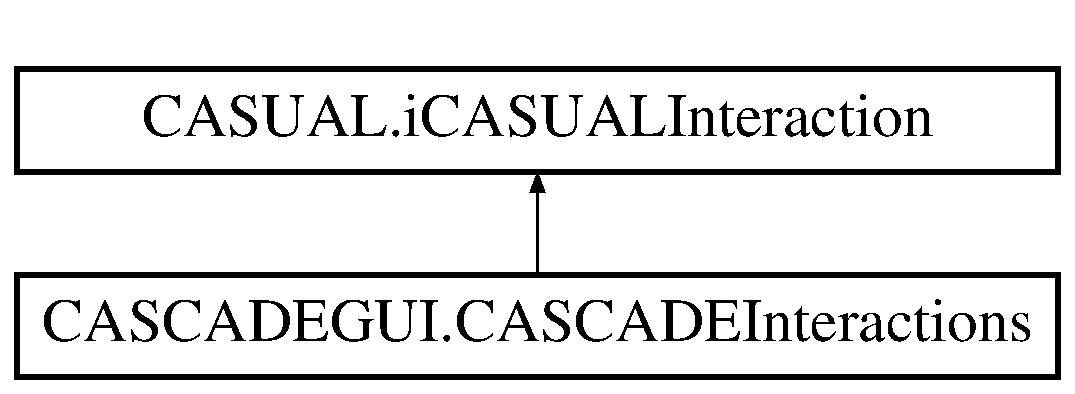
\includegraphics[height=2.000000cm]{classCASCADEGUI_1_1CASCADEInteractions}
\end{center}
\end{figure}
\subsection*{Public Member Functions}
\begin{DoxyCompactItemize}
\item 
String \hyperlink{classCASCADEGUI_1_1CASCADEInteractions_a4a7a501373e72563b00ba7ef6b4b6ecb}{display\-Message} (\hyperlink{classCASUAL_1_1CASUALMessageObject}{C\-A\-S\-U\-A\-L\-Message\-Object} message\-Object)
\end{DoxyCompactItemize}
\subsection*{Additional Inherited Members}


\subsection{Detailed Description}
\begin{DoxyAuthor}{Author}
adam 
\end{DoxyAuthor}


\subsection{Member Function Documentation}
\hypertarget{classCASCADEGUI_1_1CASCADEInteractions_a4a7a501373e72563b00ba7ef6b4b6ecb}{\index{C\-A\-S\-C\-A\-D\-E\-G\-U\-I\-::\-C\-A\-S\-C\-A\-D\-E\-Interactions@{C\-A\-S\-C\-A\-D\-E\-G\-U\-I\-::\-C\-A\-S\-C\-A\-D\-E\-Interactions}!display\-Message@{display\-Message}}
\index{display\-Message@{display\-Message}!CASCADEGUI::CASCADEInteractions@{C\-A\-S\-C\-A\-D\-E\-G\-U\-I\-::\-C\-A\-S\-C\-A\-D\-E\-Interactions}}
\subsubsection[{display\-Message}]{\setlength{\rightskip}{0pt plus 5cm}String C\-A\-S\-C\-A\-D\-E\-G\-U\-I.\-C\-A\-S\-C\-A\-D\-E\-Interactions.\-display\-Message (
\begin{DoxyParamCaption}
\item[{{\bf C\-A\-S\-U\-A\-L\-Message\-Object}}]{message\-Object}
\end{DoxyParamCaption}
)}}\label{classCASCADEGUI_1_1CASCADEInteractions_a4a7a501373e72563b00ba7ef6b4b6ecb}
Takes a message object and displays to user. To properly implement this class the display\-Message should, at a minimum handle both C\-A\-S\-U\-A\-L\-Message\-Object.\-title and C\-A\-S\-U\-A\-L\-Message\-Object.\-message\-Text.


\begin{DoxyParams}{Parameters}
{\em message\-Object} & defined by \hyperlink{namespaceCASUAL}{C\-A\-S\-U\-A\-L} \\
\hline
\end{DoxyParams}
\begin{DoxyReturn}{Returns}
string value which must be interpereted 
\end{DoxyReturn}


Implements \hyperlink{interfaceCASUAL_1_1iCASUALInteraction_a8c6697fd276aa8519caff45131c14bf4}{C\-A\-S\-U\-A\-L.\-i\-C\-A\-S\-U\-A\-L\-Interaction}.



The documentation for this class was generated from the following file\-:\begin{DoxyCompactItemize}
\item 
trunk/\-C\-A\-S\-C\-A\-D\-E/\-C\-A\-S\-C\-A\-D\-E-\/\-G\-U\-I/src/\-C\-A\-S\-C\-A\-D\-E\-G\-U\-I/C\-A\-S\-C\-A\-D\-E\-Interactions.\-java\end{DoxyCompactItemize}

\hypertarget{classCASUAL_1_1caspac_1_1Caspac}{\section{C\-A\-S\-U\-A\-L.\-caspac.\-Caspac Class Reference}
\label{classCASUAL_1_1caspac_1_1Caspac}\index{C\-A\-S\-U\-A\-L.\-caspac.\-Caspac@{C\-A\-S\-U\-A\-L.\-caspac.\-Caspac}}
}
\subsection*{Classes}
\begin{DoxyCompactItemize}
\item 
class \hyperlink{classCASUAL_1_1caspac_1_1Caspac_1_1Build}{Build}
\end{DoxyCompactItemize}
\subsection*{Public Member Functions}
\begin{DoxyCompactItemize}
\item 
\hypertarget{classCASUAL_1_1caspac_1_1Caspac_ab38e5cbb99b6d16f213340e9e61e74be}{{\bfseries Caspac} (File caspac, String temp\-Dir, int type)  throws I\-O\-Exception }\label{classCASUAL_1_1caspac_1_1Caspac_ab38e5cbb99b6d16f213340e9e61e74be}

\item 
\hypertarget{classCASUAL_1_1caspac_1_1Caspac_a5e48084a2dab585c35cbbfaa4fa9d930}{{\bfseries Caspac} (File caspac, String temp\-Dir, int type, char\mbox{[}$\,$\mbox{]} security\-Key)  throws I\-O\-Exception, Exception }\label{classCASUAL_1_1caspac_1_1Caspac_a5e48084a2dab585c35cbbfaa4fa9d930}

\item 
\hypertarget{classCASUAL_1_1caspac_1_1Caspac_add729e52bae97e76abb6274c966d0cef}{{\bfseries Caspac} (Code\-Source src, String temp\-Dir, int type)  throws I\-O\-Exception }\label{classCASUAL_1_1caspac_1_1Caspac_add729e52bae97e76abb6274c966d0cef}

\item 
\hypertarget{classCASUAL_1_1caspac_1_1Caspac_a0d0048140cf666e0a8d160f113a12b4a}{void {\bfseries set\-Active\-Script} (\hyperlink{classCASUAL_1_1caspac_1_1Script}{Script} s)}\label{classCASUAL_1_1caspac_1_1Caspac_a0d0048140cf666e0a8d160f113a12b4a}

\item 
\hypertarget{classCASUAL_1_1caspac_1_1Caspac_acb6c1d1e3d6d4e69930a0eeba2be3326}{\hyperlink{classCASUAL_1_1caspac_1_1Script}{Script} {\bfseries get\-Active\-Script} ()}\label{classCASUAL_1_1caspac_1_1Caspac_acb6c1d1e3d6d4e69930a0eeba2be3326}

\item 
void \hyperlink{classCASUAL_1_1caspac_1_1Caspac_a6368289098354e4d854ed665eb956dbe}{remove\-Script} (\hyperlink{classCASUAL_1_1caspac_1_1Script}{Script} script)
\item 
void \hyperlink{classCASUAL_1_1caspac_1_1Caspac_a872aa569a507a588786ad590b1a66d3b}{write} ()  throws I\-O\-Exception 
\item 
void \hyperlink{classCASUAL_1_1caspac_1_1Caspac_a9bbcc820fc5af56dd7e2a45908db30e6}{set\-Build} (Properties prop)
\item 
\hypertarget{classCASUAL_1_1caspac_1_1Caspac_ae8e8c0ace3ecbbfad7d731965c73288a}{void {\bfseries load\-First\-Script\-From\-C\-A\-S\-P\-A\-C} ()  throws Zip\-Exception, I\-O\-Exception }\label{classCASUAL_1_1caspac_1_1Caspac_ae8e8c0ace3ecbbfad7d731965c73288a}

\item 
\hypertarget{classCASUAL_1_1caspac_1_1Caspac_a3848e230c2ebe88fc4ab18d8cd72ef00}{void {\bfseries load\-Active\-Script} ()  throws I\-O\-Exception }\label{classCASUAL_1_1caspac_1_1Caspac_a3848e230c2ebe88fc4ab18d8cd72ef00}

\item 
void \hyperlink{classCASUAL_1_1caspac_1_1Caspac_a8dde0efbfc89cc5eba2a76bc29b2cd93}{load} ()  throws Zip\-Exception, I\-O\-Exception 
\item 
\hypertarget{classCASUAL_1_1caspac_1_1Caspac_a25eab75bfce4a2bae8fdba570cfd6058}{void {\bfseries wait\-For\-Unzip\-And\-Run} (Runnable action)}\label{classCASUAL_1_1caspac_1_1Caspac_a25eab75bfce4a2bae8fdba570cfd6058}

\item 
\hypertarget{classCASUAL_1_1caspac_1_1Caspac_ab4b478740128dbaa88b98c90355e5281}{void {\bfseries wait\-For\-Unzip\-And\-Run} (Runnable action, boolean on\-A\-Separate\-Thread, String Thread\-Name)}\label{classCASUAL_1_1caspac_1_1Caspac_ab4b478740128dbaa88b98c90355e5281}

\item 
\hypertarget{classCASUAL_1_1caspac_1_1Caspac_ae81bc5724a0bd3be2ab8883f318180c8}{void {\bfseries wait\-For\-Unzip\-Complete} ()}\label{classCASUAL_1_1caspac_1_1Caspac_ae81bc5724a0bd3be2ab8883f318180c8}

\item 
\hyperlink{classCASUAL_1_1caspac_1_1Script}{Script} \hyperlink{classCASUAL_1_1caspac_1_1Caspac_aaba95454fe20cc7b6c600f3a631866a6}{get\-Script\-By\-Filename} (String file\-Name)
\item 
String\mbox{[}$\,$\mbox{]} \hyperlink{classCASUAL_1_1caspac_1_1Caspac_a7faa66edaa415d62849653e520dce639}{get\-Script\-Names} ()
\item 
\hyperlink{classCASUAL_1_1caspac_1_1Script}{Script} \hyperlink{classCASUAL_1_1caspac_1_1Caspac_ace15ecf5d9e7e261161df7ea440d5cc5}{get\-Script\-By\-Name} (String name)
\item 
\hyperlink{classCASUAL_1_1caspac_1_1Script}{Script} \hyperlink{classCASUAL_1_1caspac_1_1Caspac_aef18425c5e00d5e2b3c4df0203a65e13}{update\-If\-Required} (\hyperlink{classCASUAL_1_1caspac_1_1Script}{Script} s)  throws Malformed\-U\-R\-L\-Exception, U\-R\-I\-Syntax\-Exception, I\-O\-Exception 
\item 
\hypertarget{classCASUAL_1_1caspac_1_1Caspac_a8d0624f21da3574c9c7b56d8be8528f9}{int {\bfseries replace\-Script\-By\-Name} (\hyperlink{classCASUAL_1_1caspac_1_1Script}{Script} s)}\label{classCASUAL_1_1caspac_1_1Caspac_a8d0624f21da3574c9c7b56d8be8528f9}

\item 
\hypertarget{classCASUAL_1_1caspac_1_1Caspac_a2f5a390c0f4f4e777fa5e2103bb8effa}{String {\bfseries to\-String} ()}\label{classCASUAL_1_1caspac_1_1Caspac_a2f5a390c0f4f4e777fa5e2103bb8effa}

\end{DoxyCompactItemize}
\subsection*{Static Public Member Functions}
\begin{DoxyCompactItemize}
\item 
\hypertarget{classCASUAL_1_1caspac_1_1Caspac_a3ed0cafff73995413d8ced1b79083d5c}{final static \hyperlink{classCASUAL_1_1caspac_1_1Caspac}{Caspac} {\bfseries make\-Generic\-Caspac} ()  throws I\-O\-Exception}\label{classCASUAL_1_1caspac_1_1Caspac_a3ed0cafff73995413d8ced1b79083d5c}

\end{DoxyCompactItemize}
\subsection*{Public Attributes}
\begin{DoxyCompactItemize}
\item 
\hypertarget{classCASUAL_1_1caspac_1_1Caspac_af2f8ec5ee442a10560736c9528196917}{final int {\bfseries type}}\label{classCASUAL_1_1caspac_1_1Caspac_af2f8ec5ee442a10560736c9528196917}

\item 
\hypertarget{classCASUAL_1_1caspac_1_1Caspac_a7ce54a828c27972ffe2736210726429d}{Buffered\-Image {\bfseries logo}}\label{classCASUAL_1_1caspac_1_1Caspac_a7ce54a828c27972ffe2736210726429d}

\item 
\hypertarget{classCASUAL_1_1caspac_1_1Caspac_a9c9f3568743699bb191d3b0451b4e2ac}{final File {\bfseries C\-A\-S\-P\-A\-C}}\label{classCASUAL_1_1caspac_1_1Caspac_a9c9f3568743699bb191d3b0451b4e2ac}

\item 
\hypertarget{classCASUAL_1_1caspac_1_1Caspac_a62673e4410829a0374ab80f2e0df5514}{final Code\-Source {\bfseries C\-A\-S\-P\-A\-Csrc}}\label{classCASUAL_1_1caspac_1_1Caspac_a62673e4410829a0374ab80f2e0df5514}

\item 
\hypertarget{classCASUAL_1_1caspac_1_1Caspac_a3f977939db32907dcf0eda3d9690f1dc}{String {\bfseries overview} = \char`\"{}\char`\"{}}\label{classCASUAL_1_1caspac_1_1Caspac_a3f977939db32907dcf0eda3d9690f1dc}

\item 
\hypertarget{classCASUAL_1_1caspac_1_1Caspac_a701528b95712562087956121c3ac32b5}{\hyperlink{classCASUAL_1_1caspac_1_1Caspac_1_1Build}{Build} {\bfseries build}}\label{classCASUAL_1_1caspac_1_1Caspac_a701528b95712562087956121c3ac32b5}

\item 
\hypertarget{classCASUAL_1_1caspac_1_1Caspac_a6defca8ee3937326a2f87a3127aba3ae}{Array\-List$<$ \hyperlink{classCASUAL_1_1caspac_1_1Script}{Script} $>$ {\bfseries scripts} = new Array\-List$<$\hyperlink{classCASUAL_1_1caspac_1_1Script}{Script}$>$()}\label{classCASUAL_1_1caspac_1_1Caspac_a6defca8ee3937326a2f87a3127aba3ae}

\item 
\hypertarget{classCASUAL_1_1caspac_1_1Caspac_a0d08f91a30c7acd212dfeca5279b1cc2}{final String {\bfseries Temp\-Folder}}\label{classCASUAL_1_1caspac_1_1Caspac_a0d08f91a30c7acd212dfeca5279b1cc2}

\item 
\hypertarget{classCASUAL_1_1caspac_1_1Caspac_aa4c916e6978c449a2193d5192d78b60e}{\hyperlink{classCASUAL_1_1Log}{Log} {\bfseries log} = new \hyperlink{classCASUAL_1_1Log}{Log}()}\label{classCASUAL_1_1caspac_1_1Caspac_aa4c916e6978c449a2193d5192d78b60e}

\item 
\hypertarget{classCASUAL_1_1caspac_1_1Caspac_a5c99fb7f34bb528167142e1c18f51b81}{boolean {\bfseries caspac\-Should\-Be\-Deleted\-After\-Extraction} = false}\label{classCASUAL_1_1caspac_1_1Caspac_a5c99fb7f34bb528167142e1c18f51b81}

\end{DoxyCompactItemize}
\subsection*{Static Public Attributes}
\begin{DoxyCompactItemize}
\item 
\hypertarget{classCASUAL_1_1caspac_1_1Caspac_aca726ea76b5b720e65183eac63c73b73}{static boolean {\bfseries debug} = false}\label{classCASUAL_1_1caspac_1_1Caspac_aca726ea76b5b720e65183eac63c73b73}

\end{DoxyCompactItemize}


\subsection{Detailed Description}
\begin{DoxyAuthor}{Author}
adam 
\end{DoxyAuthor}


\subsection{Member Function Documentation}
\hypertarget{classCASUAL_1_1caspac_1_1Caspac_aaba95454fe20cc7b6c600f3a631866a6}{\index{C\-A\-S\-U\-A\-L\-::caspac\-::\-Caspac@{C\-A\-S\-U\-A\-L\-::caspac\-::\-Caspac}!get\-Script\-By\-Filename@{get\-Script\-By\-Filename}}
\index{get\-Script\-By\-Filename@{get\-Script\-By\-Filename}!CASUAL::caspac::Caspac@{C\-A\-S\-U\-A\-L\-::caspac\-::\-Caspac}}
\subsubsection[{get\-Script\-By\-Filename}]{\setlength{\rightskip}{0pt plus 5cm}{\bf Script} C\-A\-S\-U\-A\-L.\-caspac.\-Caspac.\-get\-Script\-By\-Filename (
\begin{DoxyParamCaption}
\item[{String}]{file\-Name}
\end{DoxyParamCaption}
)}}\label{classCASUAL_1_1caspac_1_1Caspac_aaba95454fe20cc7b6c600f3a631866a6}
script instance which is being referenced


\begin{DoxyParams}{Parameters}
{\em file\-Name} & filename of script \\
\hline
\end{DoxyParams}
\begin{DoxyReturn}{Returns}
script instance of script to be processed null if not found 
\end{DoxyReturn}
\hypertarget{classCASUAL_1_1caspac_1_1Caspac_ace15ecf5d9e7e261161df7ea440d5cc5}{\index{C\-A\-S\-U\-A\-L\-::caspac\-::\-Caspac@{C\-A\-S\-U\-A\-L\-::caspac\-::\-Caspac}!get\-Script\-By\-Name@{get\-Script\-By\-Name}}
\index{get\-Script\-By\-Name@{get\-Script\-By\-Name}!CASUAL::caspac::Caspac@{C\-A\-S\-U\-A\-L\-::caspac\-::\-Caspac}}
\subsubsection[{get\-Script\-By\-Name}]{\setlength{\rightskip}{0pt plus 5cm}{\bf Script} C\-A\-S\-U\-A\-L.\-caspac.\-Caspac.\-get\-Script\-By\-Name (
\begin{DoxyParamCaption}
\item[{String}]{name}
\end{DoxyParamCaption}
)}}\label{classCASUAL_1_1caspac_1_1Caspac_ace15ecf5d9e7e261161df7ea440d5cc5}
gets script by name


\begin{DoxyParams}{Parameters}
{\em name} & name of script to be pulled \\
\hline
\end{DoxyParams}
\begin{DoxyReturn}{Returns}
\hyperlink{classCASUAL_1_1caspac_1_1Script}{Script} object or null 
\end{DoxyReturn}
\hypertarget{classCASUAL_1_1caspac_1_1Caspac_a7faa66edaa415d62849653e520dce639}{\index{C\-A\-S\-U\-A\-L\-::caspac\-::\-Caspac@{C\-A\-S\-U\-A\-L\-::caspac\-::\-Caspac}!get\-Script\-Names@{get\-Script\-Names}}
\index{get\-Script\-Names@{get\-Script\-Names}!CASUAL::caspac::Caspac@{C\-A\-S\-U\-A\-L\-::caspac\-::\-Caspac}}
\subsubsection[{get\-Script\-Names}]{\setlength{\rightskip}{0pt plus 5cm}String \mbox{[}$\,$\mbox{]} C\-A\-S\-U\-A\-L.\-caspac.\-Caspac.\-get\-Script\-Names (
\begin{DoxyParamCaption}
{}
\end{DoxyParamCaption}
)}}\label{classCASUAL_1_1caspac_1_1Caspac_a7faa66edaa415d62849653e520dce639}
returns all script names

\begin{DoxyReturn}{Returns}
list of script names 
\end{DoxyReturn}
\hypertarget{classCASUAL_1_1caspac_1_1Caspac_a8dde0efbfc89cc5eba2a76bc29b2cd93}{\index{C\-A\-S\-U\-A\-L\-::caspac\-::\-Caspac@{C\-A\-S\-U\-A\-L\-::caspac\-::\-Caspac}!load@{load}}
\index{load@{load}!CASUAL::caspac::Caspac@{C\-A\-S\-U\-A\-L\-::caspac\-::\-Caspac}}
\subsubsection[{load}]{\setlength{\rightskip}{0pt plus 5cm}void C\-A\-S\-U\-A\-L.\-caspac.\-Caspac.\-load (
\begin{DoxyParamCaption}
{}
\end{DoxyParamCaption}
) throws Zip\-Exception, I\-O\-Exception}}\label{classCASUAL_1_1caspac_1_1Caspac_a8dde0efbfc89cc5eba2a76bc29b2cd93}
loads a C\-A\-S\-P\-A\-C.\-zip file


\begin{DoxyExceptions}{Exceptions}
{\em Zip\-Exception} & \\
\hline
{\em I\-O\-Exception} & \\
\hline
\end{DoxyExceptions}
\hypertarget{classCASUAL_1_1caspac_1_1Caspac_a6368289098354e4d854ed665eb956dbe}{\index{C\-A\-S\-U\-A\-L\-::caspac\-::\-Caspac@{C\-A\-S\-U\-A\-L\-::caspac\-::\-Caspac}!remove\-Script@{remove\-Script}}
\index{remove\-Script@{remove\-Script}!CASUAL::caspac::Caspac@{C\-A\-S\-U\-A\-L\-::caspac\-::\-Caspac}}
\subsubsection[{remove\-Script}]{\setlength{\rightskip}{0pt plus 5cm}void C\-A\-S\-U\-A\-L.\-caspac.\-Caspac.\-remove\-Script (
\begin{DoxyParamCaption}
\item[{{\bf Script}}]{script}
\end{DoxyParamCaption}
)}}\label{classCASUAL_1_1caspac_1_1Caspac_a6368289098354e4d854ed665eb956dbe}
removes a script


\begin{DoxyParams}{Parameters}
{\em script} & \hyperlink{classCASUAL_1_1caspac_1_1Script}{Script} reference \\
\hline
\end{DoxyParams}
\hypertarget{classCASUAL_1_1caspac_1_1Caspac_a9bbcc820fc5af56dd7e2a45908db30e6}{\index{C\-A\-S\-U\-A\-L\-::caspac\-::\-Caspac@{C\-A\-S\-U\-A\-L\-::caspac\-::\-Caspac}!set\-Build@{set\-Build}}
\index{set\-Build@{set\-Build}!CASUAL::caspac::Caspac@{C\-A\-S\-U\-A\-L\-::caspac\-::\-Caspac}}
\subsubsection[{set\-Build}]{\setlength{\rightskip}{0pt plus 5cm}void C\-A\-S\-U\-A\-L.\-caspac.\-Caspac.\-set\-Build (
\begin{DoxyParamCaption}
\item[{Properties}]{prop}
\end{DoxyParamCaption}
)}}\label{classCASUAL_1_1caspac_1_1Caspac_a9bbcc820fc5af56dd7e2a45908db30e6}
sets build properties


\begin{DoxyParams}{Parameters}
{\em prop} & properties file \\
\hline
\end{DoxyParams}
\hypertarget{classCASUAL_1_1caspac_1_1Caspac_aef18425c5e00d5e2b3c4df0203a65e13}{\index{C\-A\-S\-U\-A\-L\-::caspac\-::\-Caspac@{C\-A\-S\-U\-A\-L\-::caspac\-::\-Caspac}!update\-If\-Required@{update\-If\-Required}}
\index{update\-If\-Required@{update\-If\-Required}!CASUAL::caspac::Caspac@{C\-A\-S\-U\-A\-L\-::caspac\-::\-Caspac}}
\subsubsection[{update\-If\-Required}]{\setlength{\rightskip}{0pt plus 5cm}{\bf Script} C\-A\-S\-U\-A\-L.\-caspac.\-Caspac.\-update\-If\-Required (
\begin{DoxyParamCaption}
\item[{{\bf Script}}]{s}
\end{DoxyParamCaption}
) throws Malformed\-U\-R\-L\-Exception, U\-R\-I\-Syntax\-Exception, I\-O\-Exception}}\label{classCASUAL_1_1caspac_1_1Caspac_aef18425c5e00d5e2b3c4df0203a65e13}
checks for updates.


\begin{DoxyParams}{Parameters}
{\em s} & \hyperlink{classCASUAL_1_1caspac_1_1Script}{Script} to be checked \\
\hline
\end{DoxyParams}
\begin{DoxyReturn}{Returns}
true if script can continue. false if halt is recommended. 
\end{DoxyReturn}

\begin{DoxyExceptions}{Exceptions}
{\em java.\-net.\-Malformed\-U\-R\-L\-Exception} & \\
\hline
{\em java.\-net.\-U\-R\-I\-Syntax\-Exception} & \\
\hline
\end{DoxyExceptions}
\hypertarget{classCASUAL_1_1caspac_1_1Caspac_a872aa569a507a588786ad590b1a66d3b}{\index{C\-A\-S\-U\-A\-L\-::caspac\-::\-Caspac@{C\-A\-S\-U\-A\-L\-::caspac\-::\-Caspac}!write@{write}}
\index{write@{write}!CASUAL::caspac::Caspac@{C\-A\-S\-U\-A\-L\-::caspac\-::\-Caspac}}
\subsubsection[{write}]{\setlength{\rightskip}{0pt plus 5cm}void C\-A\-S\-U\-A\-L.\-caspac.\-Caspac.\-write (
\begin{DoxyParamCaption}
{}
\end{DoxyParamCaption}
) throws I\-O\-Exception}}\label{classCASUAL_1_1caspac_1_1Caspac_a872aa569a507a588786ad590b1a66d3b}
writes a C\-A\-S\-P\-A\-C


\begin{DoxyExceptions}{Exceptions}
{\em I\-O\-Exception} & \\
\hline
\end{DoxyExceptions}


The documentation for this class was generated from the following file\-:\begin{DoxyCompactItemize}
\item 
trunk/\-C\-A\-S\-U\-A\-Lcore/src/\-C\-A\-S\-U\-A\-L/caspac/Caspac.\-java\end{DoxyCompactItemize}

\hypertarget{classCASPACcreator_1_1CASPACcreator}{\section{C\-A\-S\-P\-A\-Ccreator.\-C\-A\-S\-P\-A\-Ccreator Class Reference}
\label{classCASPACcreator_1_1CASPACcreator}\index{C\-A\-S\-P\-A\-Ccreator.\-C\-A\-S\-P\-A\-Ccreator@{C\-A\-S\-P\-A\-Ccreator.\-C\-A\-S\-P\-A\-Ccreator}}
}
\subsection*{Static Public Member Functions}
\begin{DoxyCompactItemize}
\item 
static void \hyperlink{classCASPACcreator_1_1CASPACcreator_a079a7e649b9589a4f7f7a26d30e3c484}{main} (String\mbox{[}$\,$\mbox{]} args)
\end{DoxyCompactItemize}
\subsection*{Public Attributes}
\begin{DoxyCompactItemize}
\item 
boolean \hyperlink{classCASPACcreator_1_1CASPACcreator_a06739ae603ad3ff397ecf3efb8d2ced5}{force} = false
\item 
boolean \hyperlink{classCASPACcreator_1_1CASPACcreator_af131ba1e4eed877fa18018c5b7304255}{ignore} = false
\end{DoxyCompactItemize}


\subsection{Detailed Description}
\begin{DoxyAuthor}{Author}
loganludington 

Adam Outler 
\end{DoxyAuthor}


\subsection{Member Function Documentation}
\hypertarget{classCASPACcreator_1_1CASPACcreator_a079a7e649b9589a4f7f7a26d30e3c484}{\index{C\-A\-S\-P\-A\-Ccreator\-::\-C\-A\-S\-P\-A\-Ccreator@{C\-A\-S\-P\-A\-Ccreator\-::\-C\-A\-S\-P\-A\-Ccreator}!main@{main}}
\index{main@{main}!CASPACcreator::CASPACcreator@{C\-A\-S\-P\-A\-Ccreator\-::\-C\-A\-S\-P\-A\-Ccreator}}
\subsubsection[{main}]{\setlength{\rightskip}{0pt plus 5cm}static void C\-A\-S\-P\-A\-Ccreator.\-C\-A\-S\-P\-A\-Ccreator.\-main (
\begin{DoxyParamCaption}
\item[{String\mbox{[}$\,$\mbox{]}}]{args}
\end{DoxyParamCaption}
)\hspace{0.3cm}{\ttfamily [static]}}}\label{classCASPACcreator_1_1CASPACcreator_a079a7e649b9589a4f7f7a26d30e3c484}

\begin{DoxyParams}{Parameters}
{\em args} & the command line arguments \\
\hline
\end{DoxyParams}


\subsection{Member Data Documentation}
\hypertarget{classCASPACcreator_1_1CASPACcreator_a06739ae603ad3ff397ecf3efb8d2ced5}{\index{C\-A\-S\-P\-A\-Ccreator\-::\-C\-A\-S\-P\-A\-Ccreator@{C\-A\-S\-P\-A\-Ccreator\-::\-C\-A\-S\-P\-A\-Ccreator}!force@{force}}
\index{force@{force}!CASPACcreator::CASPACcreator@{C\-A\-S\-P\-A\-Ccreator\-::\-C\-A\-S\-P\-A\-Ccreator}}
\subsubsection[{force}]{\setlength{\rightskip}{0pt plus 5cm}boolean C\-A\-S\-P\-A\-Ccreator.\-C\-A\-S\-P\-A\-Ccreator.\-force = false}}\label{classCASPACcreator_1_1CASPACcreator_a06739ae603ad3ff397ecf3efb8d2ced5}
force overwrite \hypertarget{classCASPACcreator_1_1CASPACcreator_af131ba1e4eed877fa18018c5b7304255}{\index{C\-A\-S\-P\-A\-Ccreator\-::\-C\-A\-S\-P\-A\-Ccreator@{C\-A\-S\-P\-A\-Ccreator\-::\-C\-A\-S\-P\-A\-Ccreator}!ignore@{ignore}}
\index{ignore@{ignore}!CASPACcreator::CASPACcreator@{C\-A\-S\-P\-A\-Ccreator\-::\-C\-A\-S\-P\-A\-Ccreator}}
\subsubsection[{ignore}]{\setlength{\rightskip}{0pt plus 5cm}boolean C\-A\-S\-P\-A\-Ccreator.\-C\-A\-S\-P\-A\-Ccreator.\-ignore = false}}\label{classCASPACcreator_1_1CASPACcreator_af131ba1e4eed877fa18018c5b7304255}
ignore missing files 

The documentation for this class was generated from the following file\-:\begin{DoxyCompactItemize}
\item 
trunk/\-C\-A\-S\-C\-A\-D\-E/\-C\-A\-S\-P\-A\-Ccreator/src/\-C\-A\-S\-P\-A\-Ccreator/C\-A\-S\-P\-A\-Ccreator.\-java\end{DoxyCompactItemize}

\hypertarget{classCASPACcreator_1_1CASPACcreatorTest}{\section{C\-A\-S\-P\-A\-Ccreator.\-C\-A\-S\-P\-A\-Ccreator\-Test Class Reference}
\label{classCASPACcreator_1_1CASPACcreatorTest}\index{C\-A\-S\-P\-A\-Ccreator.\-C\-A\-S\-P\-A\-Ccreator\-Test@{C\-A\-S\-P\-A\-Ccreator.\-C\-A\-S\-P\-A\-Ccreator\-Test}}
}
\subsection*{Static Public Member Functions}
\begin{DoxyCompactItemize}
\item 
\hypertarget{classCASPACcreator_1_1CASPACcreatorTest_a3ab0f82df4a9652e33a691427c2a75e7}{static void {\bfseries set\-Up\-Class} ()}\label{classCASPACcreator_1_1CASPACcreatorTest_a3ab0f82df4a9652e33a691427c2a75e7}

\item 
\hypertarget{classCASPACcreator_1_1CASPACcreatorTest_ac5ba5a6d730573f06968ae443f82fded}{static void {\bfseries tear\-Down\-Class} ()}\label{classCASPACcreator_1_1CASPACcreatorTest_ac5ba5a6d730573f06968ae443f82fded}

\end{DoxyCompactItemize}


\subsection{Detailed Description}
\begin{DoxyAuthor}{Author}
adam 
\end{DoxyAuthor}


The documentation for this class was generated from the following file\-:\begin{DoxyCompactItemize}
\item 
trunk/\-C\-A\-S\-C\-A\-D\-E/\-C\-A\-S\-P\-A\-Ccreator/test/\-C\-A\-S\-P\-A\-Ccreator/C\-A\-S\-P\-A\-Ccreator\-Test.\-java\end{DoxyCompactItemize}

\hypertarget{classCASUAL_1_1CASPACjUnitTest}{\section{C\-A\-S\-U\-A\-L.\-C\-A\-S\-P\-A\-Cj\-Unit\-Test Class Reference}
\label{classCASUAL_1_1CASPACjUnitTest}\index{C\-A\-S\-U\-A\-L.\-C\-A\-S\-P\-A\-Cj\-Unit\-Test@{C\-A\-S\-U\-A\-L.\-C\-A\-S\-P\-A\-Cj\-Unit\-Test}}
}
\subsection*{Public Member Functions}
\begin{DoxyCompactItemize}
\item 
\hypertarget{classCASUAL_1_1CASPACjUnitTest_a5970d891918d6e696f949f1cd8d838e6}{void {\bfseries test\-C\-A\-S\-P\-A\-C\-Operations} ()}\label{classCASUAL_1_1CASPACjUnitTest_a5970d891918d6e696f949f1cd8d838e6}

\end{DoxyCompactItemize}
\subsection*{Static Public Member Functions}
\begin{DoxyCompactItemize}
\item 
\hypertarget{classCASUAL_1_1CASPACjUnitTest_a567c4df41861b0f66301e81a4fa80d1e}{static void {\bfseries set\-Up\-Class} ()}\label{classCASUAL_1_1CASPACjUnitTest_a567c4df41861b0f66301e81a4fa80d1e}

\item 
\hypertarget{classCASUAL_1_1CASPACjUnitTest_aae59acf2bb710e6a7b0a4b8aec5f53a2}{static void {\bfseries tear\-Down\-Class} ()}\label{classCASUAL_1_1CASPACjUnitTest_aae59acf2bb710e6a7b0a4b8aec5f53a2}

\end{DoxyCompactItemize}


\subsection{Detailed Description}
\begin{DoxyAuthor}{Author}
adam 
\end{DoxyAuthor}


The documentation for this class was generated from the following file\-:\begin{DoxyCompactItemize}
\item 
trunk/\-C\-A\-S\-U\-A\-Lcore/test/\-C\-A\-S\-U\-A\-L/C\-A\-S\-P\-A\-Cj\-Unit\-Test.\-java\end{DoxyCompactItemize}

\hypertarget{classCASUAL_1_1caspac_1_1CaspacTest}{\section{C\-A\-S\-U\-A\-L.\-caspac.\-Caspac\-Test Class Reference}
\label{classCASUAL_1_1caspac_1_1CaspacTest}\index{C\-A\-S\-U\-A\-L.\-caspac.\-Caspac\-Test@{C\-A\-S\-U\-A\-L.\-caspac.\-Caspac\-Test}}
}
\subsection*{Public Member Functions}
\begin{DoxyCompactItemize}
\item 
\hypertarget{classCASUAL_1_1caspac_1_1CaspacTest_a6b7a7de2245a1ada8fa98a3b01bfd381}{void {\bfseries set\-Up} ()}\label{classCASUAL_1_1caspac_1_1CaspacTest_a6b7a7de2245a1ada8fa98a3b01bfd381}

\item 
\hypertarget{classCASUAL_1_1caspac_1_1CaspacTest_a99c80cb032c5c3d1eab471503f4d448c}{void {\bfseries tear\-Down} ()}\label{classCASUAL_1_1caspac_1_1CaspacTest_a99c80cb032c5c3d1eab471503f4d448c}

\item 
void \hyperlink{classCASUAL_1_1caspac_1_1CaspacTest_aaf1801c0e6b7492e34fae5e25a83f23c}{test\-Remove\-Script} ()
\item 
\hypertarget{classCASUAL_1_1caspac_1_1CaspacTest_a056dc6cee1499f32fbc4dcde14c62557}{void {\bfseries test\-Set\-Active\-Script} ()}\label{classCASUAL_1_1caspac_1_1CaspacTest_a056dc6cee1499f32fbc4dcde14c62557}

\item 
\hypertarget{classCASUAL_1_1caspac_1_1CaspacTest_a4c2e5ad8b61d73f007534b58e1e80b54}{void {\bfseries test\-Get\-Active\-Script} ()}\label{classCASUAL_1_1caspac_1_1CaspacTest_a4c2e5ad8b61d73f007534b58e1e80b54}

\item 
\hypertarget{classCASUAL_1_1caspac_1_1CaspacTest_a7cbc2c75a5df1d2792affaa740f95e3f}{void {\bfseries test\-Set\-Build} ()}\label{classCASUAL_1_1caspac_1_1CaspacTest_a7cbc2c75a5df1d2792affaa740f95e3f}

\item 
\hypertarget{classCASUAL_1_1caspac_1_1CaspacTest_abe5ea7f10efe1f33733f9c43a8629864}{void {\bfseries test\-Echo\-Test\-Verification} ()  throws Exception }\label{classCASUAL_1_1caspac_1_1CaspacTest_abe5ea7f10efe1f33733f9c43a8629864}

\end{DoxyCompactItemize}
\subsection*{Static Public Member Functions}
\begin{DoxyCompactItemize}
\item 
\hypertarget{classCASUAL_1_1caspac_1_1CaspacTest_aff28bc082be38caa5812996b18d6ac1a}{static void {\bfseries set\-Up\-Class} ()}\label{classCASUAL_1_1caspac_1_1CaspacTest_aff28bc082be38caa5812996b18d6ac1a}

\item 
\hypertarget{classCASUAL_1_1caspac_1_1CaspacTest_aabfd9607ccc8a2080a2d7be793bdf0f5}{static void {\bfseries tear\-Down\-Class} ()}\label{classCASUAL_1_1caspac_1_1CaspacTest_aabfd9607ccc8a2080a2d7be793bdf0f5}

\end{DoxyCompactItemize}


\subsection{Detailed Description}
\begin{DoxyAuthor}{Author}
adam 
\end{DoxyAuthor}


\subsection{Member Function Documentation}
\hypertarget{classCASUAL_1_1caspac_1_1CaspacTest_aaf1801c0e6b7492e34fae5e25a83f23c}{\index{C\-A\-S\-U\-A\-L\-::caspac\-::\-Caspac\-Test@{C\-A\-S\-U\-A\-L\-::caspac\-::\-Caspac\-Test}!test\-Remove\-Script@{test\-Remove\-Script}}
\index{test\-Remove\-Script@{test\-Remove\-Script}!CASUAL::caspac::CaspacTest@{C\-A\-S\-U\-A\-L\-::caspac\-::\-Caspac\-Test}}
\subsubsection[{test\-Remove\-Script}]{\setlength{\rightskip}{0pt plus 5cm}void C\-A\-S\-U\-A\-L.\-caspac.\-Caspac\-Test.\-test\-Remove\-Script (
\begin{DoxyParamCaption}
{}
\end{DoxyParamCaption}
)}}\label{classCASUAL_1_1caspac_1_1CaspacTest_aaf1801c0e6b7492e34fae5e25a83f23c}
Test of remove\-Script method, of class \hyperlink{classCASUAL_1_1caspac_1_1Caspac}{Caspac}. 

The documentation for this class was generated from the following file\-:\begin{DoxyCompactItemize}
\item 
trunk/\-C\-A\-S\-U\-A\-Lcore/test/\-C\-A\-S\-U\-A\-L/caspac/Caspac\-Test.\-java\end{DoxyCompactItemize}

\hypertarget{classCASUAL_1_1CASUALAboutBox}{\section{C\-A\-S\-U\-A\-L.\-C\-A\-S\-U\-A\-L\-About\-Box Class Reference}
\label{classCASUAL_1_1CASUALAboutBox}\index{C\-A\-S\-U\-A\-L.\-C\-A\-S\-U\-A\-L\-About\-Box@{C\-A\-S\-U\-A\-L.\-C\-A\-S\-U\-A\-L\-About\-Box}}
}
Inheritance diagram for C\-A\-S\-U\-A\-L.\-C\-A\-S\-U\-A\-L\-About\-Box\-:\begin{figure}[H]
\begin{center}
\leavevmode
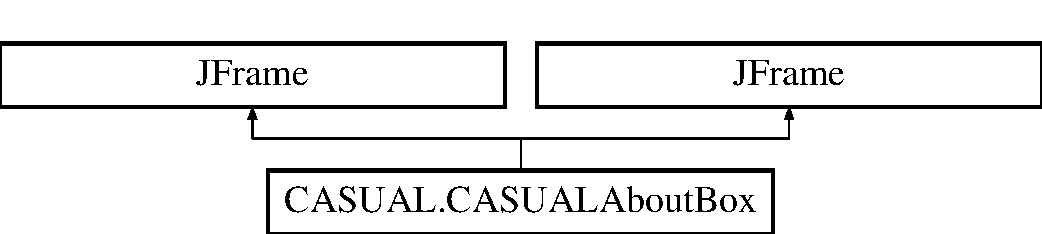
\includegraphics[height=2.000000cm]{classCASUAL_1_1CASUALAboutBox}
\end{center}
\end{figure}
\subsection*{Public Member Functions}
\begin{DoxyCompactItemize}
\item 
\hyperlink{classCASUAL_1_1CASUALAboutBox_a48d8d2dfc3dac07723d76f6e997296bd}{C\-A\-S\-U\-A\-L\-About\-Box} ()
\item 
\hyperlink{classCASUAL_1_1CASUALAboutBox_a48d8d2dfc3dac07723d76f6e997296bd}{C\-A\-S\-U\-A\-L\-About\-Box} ()
\end{DoxyCompactItemize}
\subsection*{Static Public Member Functions}
\begin{DoxyCompactItemize}
\item 
static void \hyperlink{classCASUAL_1_1CASUALAboutBox_a6cdc47b5b641579dc78c69ea028e56b0}{main} ()
\item 
static void \hyperlink{classCASUAL_1_1CASUALAboutBox_a6cdc47b5b641579dc78c69ea028e56b0}{main} ()
\end{DoxyCompactItemize}


\subsection{Detailed Description}
\begin{DoxyAuthor}{Author}
adam 
\end{DoxyAuthor}


\subsection{Constructor \& Destructor Documentation}
\hypertarget{classCASUAL_1_1CASUALAboutBox_a48d8d2dfc3dac07723d76f6e997296bd}{\index{C\-A\-S\-U\-A\-L\-::\-C\-A\-S\-U\-A\-L\-About\-Box@{C\-A\-S\-U\-A\-L\-::\-C\-A\-S\-U\-A\-L\-About\-Box}!C\-A\-S\-U\-A\-L\-About\-Box@{C\-A\-S\-U\-A\-L\-About\-Box}}
\index{C\-A\-S\-U\-A\-L\-About\-Box@{C\-A\-S\-U\-A\-L\-About\-Box}!CASUAL::CASUALAboutBox@{C\-A\-S\-U\-A\-L\-::\-C\-A\-S\-U\-A\-L\-About\-Box}}
\subsubsection[{C\-A\-S\-U\-A\-L\-About\-Box}]{\setlength{\rightskip}{0pt plus 5cm}C\-A\-S\-U\-A\-L.\-C\-A\-S\-U\-A\-L\-About\-Box.\-C\-A\-S\-U\-A\-L\-About\-Box (
\begin{DoxyParamCaption}
{}
\end{DoxyParamCaption}
)}}\label{classCASUAL_1_1CASUALAboutBox_a48d8d2dfc3dac07723d76f6e997296bd}
Creates new form C\-A\-S\-U\-A\-L\-About\-Box1 \hypertarget{classCASUAL_1_1CASUALAboutBox_a48d8d2dfc3dac07723d76f6e997296bd}{\index{C\-A\-S\-U\-A\-L\-::\-C\-A\-S\-U\-A\-L\-About\-Box@{C\-A\-S\-U\-A\-L\-::\-C\-A\-S\-U\-A\-L\-About\-Box}!C\-A\-S\-U\-A\-L\-About\-Box@{C\-A\-S\-U\-A\-L\-About\-Box}}
\index{C\-A\-S\-U\-A\-L\-About\-Box@{C\-A\-S\-U\-A\-L\-About\-Box}!CASUAL::CASUALAboutBox@{C\-A\-S\-U\-A\-L\-::\-C\-A\-S\-U\-A\-L\-About\-Box}}
\subsubsection[{C\-A\-S\-U\-A\-L\-About\-Box}]{\setlength{\rightskip}{0pt plus 5cm}C\-A\-S\-U\-A\-L.\-C\-A\-S\-U\-A\-L\-About\-Box.\-C\-A\-S\-U\-A\-L\-About\-Box (
\begin{DoxyParamCaption}
{}
\end{DoxyParamCaption}
)}}\label{classCASUAL_1_1CASUALAboutBox_a48d8d2dfc3dac07723d76f6e997296bd}
Creates new form C\-A\-S\-U\-A\-L\-About\-Box1 

\subsection{Member Function Documentation}
\hypertarget{classCASUAL_1_1CASUALAboutBox_a6cdc47b5b641579dc78c69ea028e56b0}{\index{C\-A\-S\-U\-A\-L\-::\-C\-A\-S\-U\-A\-L\-About\-Box@{C\-A\-S\-U\-A\-L\-::\-C\-A\-S\-U\-A\-L\-About\-Box}!main@{main}}
\index{main@{main}!CASUAL::CASUALAboutBox@{C\-A\-S\-U\-A\-L\-::\-C\-A\-S\-U\-A\-L\-About\-Box}}
\subsubsection[{main}]{\setlength{\rightskip}{0pt plus 5cm}static void C\-A\-S\-U\-A\-L.\-C\-A\-S\-U\-A\-L\-About\-Box.\-main (
\begin{DoxyParamCaption}
{}
\end{DoxyParamCaption}
)\hspace{0.3cm}{\ttfamily [static]}}}\label{classCASUAL_1_1CASUALAboutBox_a6cdc47b5b641579dc78c69ea028e56b0}

\begin{DoxyParams}{Parameters}
{\em args} & the command line arguments \\
\hline
\end{DoxyParams}
\hypertarget{classCASUAL_1_1CASUALAboutBox_a6cdc47b5b641579dc78c69ea028e56b0}{\index{C\-A\-S\-U\-A\-L\-::\-C\-A\-S\-U\-A\-L\-About\-Box@{C\-A\-S\-U\-A\-L\-::\-C\-A\-S\-U\-A\-L\-About\-Box}!main@{main}}
\index{main@{main}!CASUAL::CASUALAboutBox@{C\-A\-S\-U\-A\-L\-::\-C\-A\-S\-U\-A\-L\-About\-Box}}
\subsubsection[{main}]{\setlength{\rightskip}{0pt plus 5cm}static void C\-A\-S\-U\-A\-L.\-C\-A\-S\-U\-A\-L\-About\-Box.\-main (
\begin{DoxyParamCaption}
{}
\end{DoxyParamCaption}
)\hspace{0.3cm}{\ttfamily [static]}}}\label{classCASUAL_1_1CASUALAboutBox_a6cdc47b5b641579dc78c69ea028e56b0}

\begin{DoxyParams}{Parameters}
{\em args} & the command line arguments \\
\hline
\end{DoxyParams}


The documentation for this class was generated from the following files\-:\begin{DoxyCompactItemize}
\item 
branches/\-C\-A\-S\-U\-A\-L-\/\-Headless/\-G\-U\-I/src/\-C\-A\-S\-U\-A\-L/C\-A\-S\-U\-A\-L\-About\-Box.\-java\item 
branches/\-Testing\-Branch/\-G\-Doc/src/\-C\-A\-S\-U\-A\-L/C\-A\-S\-U\-A\-L\-About\-Box.\-java\end{DoxyCompactItemize}

\hypertarget{classCASUAL_1_1CASUALApp}{\section{C\-A\-S\-U\-A\-L.\-C\-A\-S\-U\-A\-L\-App Class Reference}
\label{classCASUAL_1_1CASUALApp}\index{C\-A\-S\-U\-A\-L.\-C\-A\-S\-U\-A\-L\-App@{C\-A\-S\-U\-A\-L.\-C\-A\-S\-U\-A\-L\-App}}
}
Inheritance diagram for C\-A\-S\-U\-A\-L.\-C\-A\-S\-U\-A\-L\-App\-:\begin{figure}[H]
\begin{center}
\leavevmode
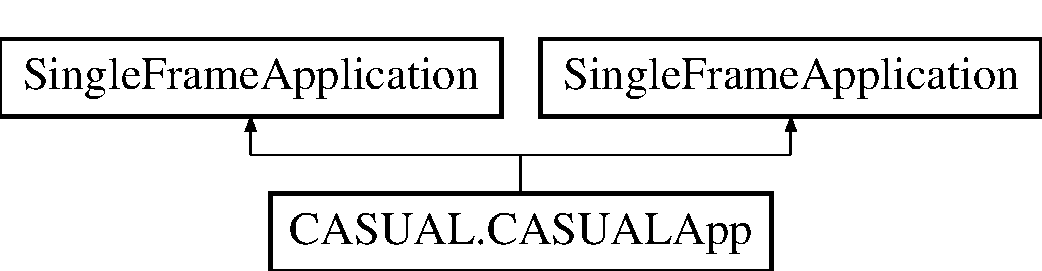
\includegraphics[height=2.000000cm]{classCASUAL_1_1CASUALApp}
\end{center}
\end{figure}
\subsection*{Static Public Member Functions}
\begin{DoxyCompactItemize}
\item 
static \hyperlink{classCASUAL_1_1CASUALApp}{C\-A\-S\-U\-A\-L\-App} \hyperlink{classCASUAL_1_1CASUALApp_a10428ae7a0decfd58a8089abba4c2ec3}{get\-Application} ()
\item 
static void \hyperlink{classCASUAL_1_1CASUALApp_ae70d2201eea0faed56373ae468d835a3}{main} (String\mbox{[}$\,$\mbox{]} args)
\item 
static \hyperlink{classCASUAL_1_1CASUALApp}{C\-A\-S\-U\-A\-L\-App} \hyperlink{classCASUAL_1_1CASUALApp_a10428ae7a0decfd58a8089abba4c2ec3}{get\-Application} ()
\item 
static void \hyperlink{classCASUAL_1_1CASUALApp_ae70d2201eea0faed56373ae468d835a3}{main} (String\mbox{[}$\,$\mbox{]} args)
\end{DoxyCompactItemize}
\subsection*{Protected Member Functions}
\begin{DoxyCompactItemize}
\item 
void \hyperlink{classCASUAL_1_1CASUALApp_a599fe9852fc5a20cfc144465ab9a6a06}{startup} ()
\item 
void \hyperlink{classCASUAL_1_1CASUALApp_adf38955dc957953f82eb4c0d2cefa6fe}{configure\-Window} (java.\-awt.\-Window root)
\item 
void \hyperlink{classCASUAL_1_1CASUALApp_a599fe9852fc5a20cfc144465ab9a6a06}{startup} ()
\item 
void \hyperlink{classCASUAL_1_1CASUALApp_adf38955dc957953f82eb4c0d2cefa6fe}{configure\-Window} (java.\-awt.\-Window root)
\end{DoxyCompactItemize}


\subsection{Detailed Description}
The main class of the application. 

\subsection{Member Function Documentation}
\hypertarget{classCASUAL_1_1CASUALApp_adf38955dc957953f82eb4c0d2cefa6fe}{\index{C\-A\-S\-U\-A\-L\-::\-C\-A\-S\-U\-A\-L\-App@{C\-A\-S\-U\-A\-L\-::\-C\-A\-S\-U\-A\-L\-App}!configure\-Window@{configure\-Window}}
\index{configure\-Window@{configure\-Window}!CASUAL::CASUALApp@{C\-A\-S\-U\-A\-L\-::\-C\-A\-S\-U\-A\-L\-App}}
\subsubsection[{configure\-Window}]{\setlength{\rightskip}{0pt plus 5cm}void C\-A\-S\-U\-A\-L.\-C\-A\-S\-U\-A\-L\-App.\-configure\-Window (
\begin{DoxyParamCaption}
\item[{java.\-awt.\-Window}]{root}
\end{DoxyParamCaption}
)\hspace{0.3cm}{\ttfamily [protected]}}}\label{classCASUAL_1_1CASUALApp_adf38955dc957953f82eb4c0d2cefa6fe}
This method is to initialize the specified window by injecting resources. Windows shown in our application come fully initialized from the G\-U\-I builder, so this additional configuration is not needed. \hypertarget{classCASUAL_1_1CASUALApp_adf38955dc957953f82eb4c0d2cefa6fe}{\index{C\-A\-S\-U\-A\-L\-::\-C\-A\-S\-U\-A\-L\-App@{C\-A\-S\-U\-A\-L\-::\-C\-A\-S\-U\-A\-L\-App}!configure\-Window@{configure\-Window}}
\index{configure\-Window@{configure\-Window}!CASUAL::CASUALApp@{C\-A\-S\-U\-A\-L\-::\-C\-A\-S\-U\-A\-L\-App}}
\subsubsection[{configure\-Window}]{\setlength{\rightskip}{0pt plus 5cm}void C\-A\-S\-U\-A\-L.\-C\-A\-S\-U\-A\-L\-App.\-configure\-Window (
\begin{DoxyParamCaption}
\item[{java.\-awt.\-Window}]{root}
\end{DoxyParamCaption}
)\hspace{0.3cm}{\ttfamily [protected]}}}\label{classCASUAL_1_1CASUALApp_adf38955dc957953f82eb4c0d2cefa6fe}
This method is to initialize the specified window by injecting resources. Windows shown in our application come fully initialized from the G\-U\-I builder, so this additional configuration is not needed. \hypertarget{classCASUAL_1_1CASUALApp_a10428ae7a0decfd58a8089abba4c2ec3}{\index{C\-A\-S\-U\-A\-L\-::\-C\-A\-S\-U\-A\-L\-App@{C\-A\-S\-U\-A\-L\-::\-C\-A\-S\-U\-A\-L\-App}!get\-Application@{get\-Application}}
\index{get\-Application@{get\-Application}!CASUAL::CASUALApp@{C\-A\-S\-U\-A\-L\-::\-C\-A\-S\-U\-A\-L\-App}}
\subsubsection[{get\-Application}]{\setlength{\rightskip}{0pt plus 5cm}static {\bf C\-A\-S\-U\-A\-L\-App} C\-A\-S\-U\-A\-L.\-C\-A\-S\-U\-A\-L\-App.\-get\-Application (
\begin{DoxyParamCaption}
{}
\end{DoxyParamCaption}
)\hspace{0.3cm}{\ttfamily [static]}}}\label{classCASUAL_1_1CASUALApp_a10428ae7a0decfd58a8089abba4c2ec3}
A convenient static getter for the application instance.

\begin{DoxyReturn}{Returns}
the instance of N\-A\-R\-S\-App 
\end{DoxyReturn}
\hypertarget{classCASUAL_1_1CASUALApp_a10428ae7a0decfd58a8089abba4c2ec3}{\index{C\-A\-S\-U\-A\-L\-::\-C\-A\-S\-U\-A\-L\-App@{C\-A\-S\-U\-A\-L\-::\-C\-A\-S\-U\-A\-L\-App}!get\-Application@{get\-Application}}
\index{get\-Application@{get\-Application}!CASUAL::CASUALApp@{C\-A\-S\-U\-A\-L\-::\-C\-A\-S\-U\-A\-L\-App}}
\subsubsection[{get\-Application}]{\setlength{\rightskip}{0pt plus 5cm}static {\bf C\-A\-S\-U\-A\-L\-App} C\-A\-S\-U\-A\-L.\-C\-A\-S\-U\-A\-L\-App.\-get\-Application (
\begin{DoxyParamCaption}
{}
\end{DoxyParamCaption}
)\hspace{0.3cm}{\ttfamily [static]}}}\label{classCASUAL_1_1CASUALApp_a10428ae7a0decfd58a8089abba4c2ec3}
A convenient static getter for the application instance.

\begin{DoxyReturn}{Returns}
the instance of N\-A\-R\-S\-App 
\end{DoxyReturn}
\hypertarget{classCASUAL_1_1CASUALApp_ae70d2201eea0faed56373ae468d835a3}{\index{C\-A\-S\-U\-A\-L\-::\-C\-A\-S\-U\-A\-L\-App@{C\-A\-S\-U\-A\-L\-::\-C\-A\-S\-U\-A\-L\-App}!main@{main}}
\index{main@{main}!CASUAL::CASUALApp@{C\-A\-S\-U\-A\-L\-::\-C\-A\-S\-U\-A\-L\-App}}
\subsubsection[{main}]{\setlength{\rightskip}{0pt plus 5cm}static void C\-A\-S\-U\-A\-L.\-C\-A\-S\-U\-A\-L\-App.\-main (
\begin{DoxyParamCaption}
\item[{String\mbox{[}$\,$\mbox{]}}]{args}
\end{DoxyParamCaption}
)\hspace{0.3cm}{\ttfamily [static]}}}\label{classCASUAL_1_1CASUALApp_ae70d2201eea0faed56373ae468d835a3}
Main method launching the application. \hypertarget{classCASUAL_1_1CASUALApp_ae70d2201eea0faed56373ae468d835a3}{\index{C\-A\-S\-U\-A\-L\-::\-C\-A\-S\-U\-A\-L\-App@{C\-A\-S\-U\-A\-L\-::\-C\-A\-S\-U\-A\-L\-App}!main@{main}}
\index{main@{main}!CASUAL::CASUALApp@{C\-A\-S\-U\-A\-L\-::\-C\-A\-S\-U\-A\-L\-App}}
\subsubsection[{main}]{\setlength{\rightskip}{0pt plus 5cm}static void C\-A\-S\-U\-A\-L.\-C\-A\-S\-U\-A\-L\-App.\-main (
\begin{DoxyParamCaption}
\item[{String\mbox{[}$\,$\mbox{]}}]{args}
\end{DoxyParamCaption}
)\hspace{0.3cm}{\ttfamily [static]}}}\label{classCASUAL_1_1CASUALApp_ae70d2201eea0faed56373ae468d835a3}
Main method launching the application. \hypertarget{classCASUAL_1_1CASUALApp_a599fe9852fc5a20cfc144465ab9a6a06}{\index{C\-A\-S\-U\-A\-L\-::\-C\-A\-S\-U\-A\-L\-App@{C\-A\-S\-U\-A\-L\-::\-C\-A\-S\-U\-A\-L\-App}!startup@{startup}}
\index{startup@{startup}!CASUAL::CASUALApp@{C\-A\-S\-U\-A\-L\-::\-C\-A\-S\-U\-A\-L\-App}}
\subsubsection[{startup}]{\setlength{\rightskip}{0pt plus 5cm}void C\-A\-S\-U\-A\-L.\-C\-A\-S\-U\-A\-L\-App.\-startup (
\begin{DoxyParamCaption}
{}
\end{DoxyParamCaption}
)\hspace{0.3cm}{\ttfamily [protected]}}}\label{classCASUAL_1_1CASUALApp_a599fe9852fc5a20cfc144465ab9a6a06}
At startup create and show the main frame of the application. \hypertarget{classCASUAL_1_1CASUALApp_a599fe9852fc5a20cfc144465ab9a6a06}{\index{C\-A\-S\-U\-A\-L\-::\-C\-A\-S\-U\-A\-L\-App@{C\-A\-S\-U\-A\-L\-::\-C\-A\-S\-U\-A\-L\-App}!startup@{startup}}
\index{startup@{startup}!CASUAL::CASUALApp@{C\-A\-S\-U\-A\-L\-::\-C\-A\-S\-U\-A\-L\-App}}
\subsubsection[{startup}]{\setlength{\rightskip}{0pt plus 5cm}void C\-A\-S\-U\-A\-L.\-C\-A\-S\-U\-A\-L\-App.\-startup (
\begin{DoxyParamCaption}
{}
\end{DoxyParamCaption}
)\hspace{0.3cm}{\ttfamily [protected]}}}\label{classCASUAL_1_1CASUALApp_a599fe9852fc5a20cfc144465ab9a6a06}
At startup create and show the main frame of the application. 

The documentation for this class was generated from the following files\-:\begin{DoxyCompactItemize}
\item 
branches/\-C\-A\-S\-U\-A\-L-\/\-Headless/\-G\-U\-I/src/\-C\-A\-S\-U\-A\-L/C\-A\-S\-U\-A\-L\-App.\-java\item 
branches/\-Testing\-Branch/\-G\-Doc/src/\-C\-A\-S\-U\-A\-L/C\-A\-S\-U\-A\-L\-App.\-java\end{DoxyCompactItemize}

\hypertarget{classCASUAL_1_1CASUALAudioSystem}{\section{C\-A\-S\-U\-A\-L.\-C\-A\-S\-U\-A\-L\-Audio\-System Class Reference}
\label{classCASUAL_1_1CASUALAudioSystem}\index{C\-A\-S\-U\-A\-L.\-C\-A\-S\-U\-A\-L\-Audio\-System@{C\-A\-S\-U\-A\-L.\-C\-A\-S\-U\-A\-L\-Audio\-System}}
}
\subsection*{Static Public Member Functions}
\begin{DoxyCompactItemize}
\item 
\hypertarget{classCASUAL_1_1CASUALAudioSystem_af178e07e8a55d9d7d04288394649a824}{static synchronized void {\bfseries play\-Sound} (final String U\-R\-L)}\label{classCASUAL_1_1CASUALAudioSystem_af178e07e8a55d9d7d04288394649a824}

\item 
\hypertarget{classCASUAL_1_1CASUALAudioSystem_ac8c3c01ac6a5e1a3eb99e853734d0a9d}{static synchronized void {\bfseries play\-Multiple\-Input\-Streams} (final String\mbox{[}$\,$\mbox{]} U\-R\-Ls)}\label{classCASUAL_1_1CASUALAudioSystem_ac8c3c01ac6a5e1a3eb99e853734d0a9d}

\item 
\hypertarget{classCASUAL_1_1CASUALAudioSystem_af178e07e8a55d9d7d04288394649a824}{static synchronized void {\bfseries play\-Sound} (final String U\-R\-L)}\label{classCASUAL_1_1CASUALAudioSystem_af178e07e8a55d9d7d04288394649a824}

\item 
\hypertarget{classCASUAL_1_1CASUALAudioSystem_ac8c3c01ac6a5e1a3eb99e853734d0a9d}{static synchronized void {\bfseries play\-Multiple\-Input\-Streams} (final String\mbox{[}$\,$\mbox{]} U\-R\-Ls)}\label{classCASUAL_1_1CASUALAudioSystem_ac8c3c01ac6a5e1a3eb99e853734d0a9d}

\end{DoxyCompactItemize}


\subsection{Detailed Description}
\hyperlink{classCASUAL_1_1CASUALAudioSystem}{C\-A\-S\-U\-A\-L\-Audio\-System} handles Sounds

\begin{DoxyAuthor}{Author}
Adam Outler \href{mailto:adamoutler@gmail.com}{\tt adamoutler@gmail.\-com} 
\end{DoxyAuthor}


The documentation for this class was generated from the following files\-:\begin{DoxyCompactItemize}
\item 
branches/\-C\-A\-S\-U\-A\-L-\/\-Headless/\-G\-U\-I/src/\-C\-A\-S\-U\-A\-L/C\-A\-S\-U\-A\-L\-Audio\-System.\-java\item 
branches/\-Testing\-Branch/\-G\-Doc/src/\-C\-A\-S\-U\-A\-L/C\-A\-S\-U\-A\-L\-Audio\-System.\-java\end{DoxyCompactItemize}

\hypertarget{classCASUAL_1_1CASUALConnectionStatusMonitor}{\section{C\-A\-S\-U\-A\-L.\-C\-A\-S\-U\-A\-L\-Connection\-Status\-Monitor Class Reference}
\label{classCASUAL_1_1CASUALConnectionStatusMonitor}\index{C\-A\-S\-U\-A\-L.\-C\-A\-S\-U\-A\-L\-Connection\-Status\-Monitor@{C\-A\-S\-U\-A\-L.\-C\-A\-S\-U\-A\-L\-Connection\-Status\-Monitor}}
}
\subsection*{Static Public Member Functions}
\begin{DoxyCompactItemize}
\item 
static void \hyperlink{classCASUAL_1_1CASUALConnectionStatusMonitor_a8b18170642eaa60caadf87c180a4b3c8}{set\-Mode} (String mode)
\end{DoxyCompactItemize}
\subsection*{Static Public Attributes}
\begin{DoxyCompactItemize}
\item 
\hypertarget{classCASUAL_1_1CASUALConnectionStatusMonitor_a90e99917eda2f6d4ac56313ebb3fd4c7}{static final int {\bfseries O\-N\-E\-\_\-\-S\-E\-C\-O\-N\-D} = 1000}\label{classCASUAL_1_1CASUALConnectionStatusMonitor_a90e99917eda2f6d4ac56313ebb3fd4c7}

\item 
\hypertarget{classCASUAL_1_1CASUALConnectionStatusMonitor_a1c9e576e98ffbd5cd92060fb3dbf69ac}{static String\mbox{[}$\,$\mbox{]} {\bfseries Device\-Tracker}}\label{classCASUAL_1_1CASUALConnectionStatusMonitor_a1c9e576e98ffbd5cd92060fb3dbf69ac}

\item 
\hypertarget{classCASUAL_1_1CASUALConnectionStatusMonitor_a65f45d24cba3f9eed0d1837798330c58}{static int {\bfseries adb\-Locked\-Up} = 0}\label{classCASUAL_1_1CASUALConnectionStatusMonitor_a65f45d24cba3f9eed0d1837798330c58}

\item 
static Timer {\bfseries Device\-Check}
\end{DoxyCompactItemize}


\subsection{Detailed Description}
\begin{DoxyAuthor}{Author}
Adam Outler \href{mailto:adamoutler@gmail.com}{\tt adamoutler@gmail.\-com} 
\end{DoxyAuthor}


\subsection{Member Function Documentation}
\hypertarget{classCASUAL_1_1CASUALConnectionStatusMonitor_a8b18170642eaa60caadf87c180a4b3c8}{\index{C\-A\-S\-U\-A\-L\-::\-C\-A\-S\-U\-A\-L\-Connection\-Status\-Monitor@{C\-A\-S\-U\-A\-L\-::\-C\-A\-S\-U\-A\-L\-Connection\-Status\-Monitor}!set\-Mode@{set\-Mode}}
\index{set\-Mode@{set\-Mode}!CASUAL::CASUALConnectionStatusMonitor@{C\-A\-S\-U\-A\-L\-::\-C\-A\-S\-U\-A\-L\-Connection\-Status\-Monitor}}
\subsubsection[{set\-Mode}]{\setlength{\rightskip}{0pt plus 5cm}static void C\-A\-S\-U\-A\-L.\-C\-A\-S\-U\-A\-L\-Connection\-Status\-Monitor.\-set\-Mode (
\begin{DoxyParamCaption}
\item[{String}]{mode}
\end{DoxyParamCaption}
)\hspace{0.3cm}{\ttfamily [static]}}}\label{classCASUAL_1_1CASUALConnectionStatusMonitor_a8b18170642eaa60caadf87c180a4b3c8}
Starts and stops the A\-D\-B timer reference with Statics.\-casual\-Connection\-Status\-Monitor.\-Device\-Check O\-N\-L\-Y; 
\begin{DoxyParams}{Parameters}
{\em mode} & sets the monitoring mode \\
\hline
\end{DoxyParams}


\subsection{Member Data Documentation}
\hypertarget{classCASUAL_1_1CASUALConnectionStatusMonitor_a5d0a815804a5a296a4b8715e852f9b44}{\index{C\-A\-S\-U\-A\-L\-::\-C\-A\-S\-U\-A\-L\-Connection\-Status\-Monitor@{C\-A\-S\-U\-A\-L\-::\-C\-A\-S\-U\-A\-L\-Connection\-Status\-Monitor}!Device\-Check@{Device\-Check}}
\index{Device\-Check@{Device\-Check}!CASUAL::CASUALConnectionStatusMonitor@{C\-A\-S\-U\-A\-L\-::\-C\-A\-S\-U\-A\-L\-Connection\-Status\-Monitor}}
\subsubsection[{Device\-Check}]{\setlength{\rightskip}{0pt plus 5cm}Timer C\-A\-S\-U\-A\-L.\-C\-A\-S\-U\-A\-L\-Connection\-Status\-Monitor.\-Device\-Check\hspace{0.3cm}{\ttfamily [static]}}}\label{classCASUAL_1_1CASUALConnectionStatusMonitor_a5d0a815804a5a296a4b8715e852f9b44}
{\bfseries Initial value\-:}
\begin{DoxyCode}
= \textcolor{keyword}{new} Timer(TIMERINTERVAL, \textcolor{keyword}{new} ActionListener() \{
        @Override
        \textcolor{keyword}{public} \textcolor{keywordtype}{void} actionPerformed(ActionEvent evt) \{
            \textcolor{keywordflow}{if} (mode.equals(\textcolor{stringliteral}{"qprst"})) \{
                
            \} \textcolor{keywordflow}{else} \{  
                Thread t = \textcolor{keyword}{new} Thread(adbDeviceCheck);
                t.setName(\textcolor{stringliteral}{"Device Monitor"});
                t.start();
            \}
        \}
    \})
\end{DoxyCode}


The documentation for this class was generated from the following files\-:\begin{DoxyCompactItemize}
\item 
branches/\-C\-A\-S\-U\-A\-L-\/\-Headless/\-G\-U\-I/src/\-C\-A\-S\-U\-A\-L/C\-A\-S\-U\-A\-L\-Connection\-Status\-Monitor.\-java\item 
branches/\-Testing\-Branch/\-G\-Doc/src/\-C\-A\-S\-U\-A\-L/C\-A\-S\-U\-A\-L\-Connection\-Status\-Monitor.\-java\item 
trunk/\-C\-A\-S\-U\-A\-Lcore/src/\-C\-A\-S\-U\-A\-L/C\-A\-S\-U\-A\-L\-Connection\-Status\-Monitor.\-java\end{DoxyCompactItemize}

\hypertarget{classCASUAL_1_1CASUALDataBridge}{\section{C\-A\-S\-U\-A\-L.\-C\-A\-S\-U\-A\-L\-Data\-Bridge Class Reference}
\label{classCASUAL_1_1CASUALDataBridge}\index{C\-A\-S\-U\-A\-L.\-C\-A\-S\-U\-A\-L\-Data\-Bridge@{C\-A\-S\-U\-A\-L.\-C\-A\-S\-U\-A\-L\-Data\-Bridge}}
}
\subsection*{Classes}
\begin{DoxyCompactItemize}
\item 
class {\bfseries Device\-Side}
\end{DoxyCompactItemize}
\subsection*{Public Member Functions}
\begin{DoxyCompactItemize}
\item 
\hypertarget{classCASUAL_1_1CASUALDataBridge_a5e0d967936b2a364514ec36e3a9862e2}{synchronized String {\bfseries get\-File} (String remote\-File\-Name, File f)  throws I\-O\-Exception, Interrupted\-Exception }\label{classCASUAL_1_1CASUALDataBridge_a5e0d967936b2a364514ec36e3a9862e2}

\item 
\hypertarget{classCASUAL_1_1CASUALDataBridge_ae83af46e7e309f4f800266408cd84f63}{synchronized long {\bfseries send\-String} (String send, String remote\-File\-Name)  throws Interrupted\-Exception, Socket\-Exception, I\-O\-Exception }\label{classCASUAL_1_1CASUALDataBridge_ae83af46e7e309f4f800266408cd84f63}

\item 
\hypertarget{classCASUAL_1_1CASUALDataBridge_a11dbfc8a7894becee079c99dcbb36627}{synchronized long {\bfseries send\-File} (File f, String remote\-File\-Name)  throws File\-Not\-Found\-Exception, Exception }\label{classCASUAL_1_1CASUALDataBridge_a11dbfc8a7894becee079c99dcbb36627}

\item 
\hypertarget{classCASUAL_1_1CASUALDataBridge_a5e9f37467297dedeecf7f3f2a0ac1abf}{synchronized long {\bfseries send\-Stream} (final Input\-Stream input, final String remote\-File\-Name)  throws Interrupted\-Exception, Socket\-Exception, I\-O\-Exception }\label{classCASUAL_1_1CASUALDataBridge_a5e9f37467297dedeecf7f3f2a0ac1abf}

\end{DoxyCompactItemize}
\subsection*{Static Public Attributes}
\begin{DoxyCompactItemize}
\item 
\hypertarget{classCASUAL_1_1CASUALDataBridge_a3f1cf8cee5785332eac767cbd20041f2}{static boolean {\bfseries commanded\-Shutdown} =false}\label{classCASUAL_1_1CASUALDataBridge_a3f1cf8cee5785332eac767cbd20041f2}

\item 
static Timer \hyperlink{classCASUAL_1_1CASUALDataBridge_a2f95d8ec4d06f75bf5e089658604e46d}{timeout\-Watchdog}
\end{DoxyCompactItemize}


\subsection{Detailed Description}
\begin{DoxyAuthor}{Author}
adam 
\end{DoxyAuthor}


\subsection{Member Data Documentation}
\hypertarget{classCASUAL_1_1CASUALDataBridge_a2f95d8ec4d06f75bf5e089658604e46d}{\index{C\-A\-S\-U\-A\-L\-::\-C\-A\-S\-U\-A\-L\-Data\-Bridge@{C\-A\-S\-U\-A\-L\-::\-C\-A\-S\-U\-A\-L\-Data\-Bridge}!timeout\-Watchdog@{timeout\-Watchdog}}
\index{timeout\-Watchdog@{timeout\-Watchdog}!CASUAL::CASUALDataBridge@{C\-A\-S\-U\-A\-L\-::\-C\-A\-S\-U\-A\-L\-Data\-Bridge}}
\subsubsection[{timeout\-Watchdog}]{\setlength{\rightskip}{0pt plus 5cm}Timer C\-A\-S\-U\-A\-L.\-C\-A\-S\-U\-A\-L\-Data\-Bridge.\-timeout\-Watchdog\hspace{0.3cm}{\ttfamily [static]}}}\label{classCASUAL_1_1CASUALDataBridge_a2f95d8ec4d06f75bf5e089658604e46d}
{\bfseries Initial value\-:}
\begin{DoxyCode}
= \textcolor{keyword}{new} Timer(WATCHDOGINTERVAL, \textcolor{keyword}{new} ActionListener() \{
        @Override
        \textcolor{keyword}{public} \textcolor{keywordtype}{void} actionPerformed(ActionEvent evt) \{
            \textcolor{keywordflow}{if} (lastbytes == bytes) \{
                \textcolor{keywordflow}{try} \{
                    \textcolor{keyword}{new} Log().level0Error(\textcolor{stringliteral}{"Failed to send file.  Timeout. Bytes:"} + bytes + \textcolor{stringliteral}{" Message:"} + 
      deviceSideMessage);
                    deviceReadyForReceive = \textcolor{keyword}{false};
                    shutdownBecauseOfError = \textcolor{keyword}{true};
                    \hyperlink{classCASUAL_1_1CASUALDataBridge_a2f95d8ec4d06f75bf5e089658604e46d}{timeoutWatchdog}.stop();
                    \textcolor{keywordflow}{throw} \textcolor{keyword}{new} TimeoutException();
                \} \textcolor{keywordflow}{catch} (TimeoutException ex) \{
                    Logger.getLogger(CASUALDataBridge.class.getName()).log(Level.SEVERE, null, ex);
                \}

            \} \textcolor{keywordflow}{else} \{
                lastbytes = bytes;
                Statics.setStatus(status + \textcolor{stringliteral}{" "} + bytes);
            \}

        \}
    \})
\end{DoxyCode}
timeout\-Watchdog checks every W\-A\-T\-C\-H\-D\-O\-G\-I\-N\-T\-E\-R\-V\-A\-L millis to verify bytes have increased. If bytes have not increased, it throws an error and shuts things down. This is used to detect a broken connection. 

The documentation for this class was generated from the following file\-:\begin{DoxyCompactItemize}
\item 
trunk/\-C\-A\-S\-U\-A\-Lcore/src/\-C\-A\-S\-U\-A\-L/C\-A\-S\-U\-A\-L\-Data\-Bridge.\-java\end{DoxyCompactItemize}

\hypertarget{classCASUAL_1_1CASUALDataBridgeTest}{\section{C\-A\-S\-U\-A\-L.\-C\-A\-S\-U\-A\-L\-Data\-Bridge\-Test Class Reference}
\label{classCASUAL_1_1CASUALDataBridgeTest}\index{C\-A\-S\-U\-A\-L.\-C\-A\-S\-U\-A\-L\-Data\-Bridge\-Test@{C\-A\-S\-U\-A\-L.\-C\-A\-S\-U\-A\-L\-Data\-Bridge\-Test}}
}
\subsection*{Public Member Functions}
\begin{DoxyCompactItemize}
\item 
\hypertarget{classCASUAL_1_1CASUALDataBridgeTest_a6cbfa475ba06d452fcc0184704e1db26}{void {\bfseries set\-Up} ()}\label{classCASUAL_1_1CASUALDataBridgeTest_a6cbfa475ba06d452fcc0184704e1db26}

\item 
\hypertarget{classCASUAL_1_1CASUALDataBridgeTest_abd31aa43241e809aa8beefe78f632353}{void {\bfseries tear\-Down} ()}\label{classCASUAL_1_1CASUALDataBridgeTest_abd31aa43241e809aa8beefe78f632353}

\item 
\hypertarget{classCASUAL_1_1CASUALDataBridgeTest_aae8e888442289e5a5fbe181ea4252f65}{void {\bfseries test\-Send\-String} ()}\label{classCASUAL_1_1CASUALDataBridgeTest_aae8e888442289e5a5fbe181ea4252f65}

\item 
\hypertarget{classCASUAL_1_1CASUALDataBridgeTest_ad5e3e12bb87e858964deae861531cd88}{void {\bfseries test\-Send\-File} ()  throws Exception }\label{classCASUAL_1_1CASUALDataBridgeTest_ad5e3e12bb87e858964deae861531cd88}

\item 
\hypertarget{classCASUAL_1_1CASUALDataBridgeTest_af34007577ea765e71f5c44e4680ed8a2}{void {\bfseries test\-Get\-File} ()  throws Exception }\label{classCASUAL_1_1CASUALDataBridgeTest_af34007577ea765e71f5c44e4680ed8a2}

\item 
\hypertarget{classCASUAL_1_1CASUALDataBridgeTest_a5fbee8b2fbfc1dfe930c2eda88c00021}{void {\bfseries test\-Send\-Stream} ()  throws Exception }\label{classCASUAL_1_1CASUALDataBridgeTest_a5fbee8b2fbfc1dfe930c2eda88c00021}

\end{DoxyCompactItemize}


\subsection{Detailed Description}
\begin{DoxyAuthor}{Author}
adam 
\end{DoxyAuthor}


The documentation for this class was generated from the following file\-:\begin{DoxyCompactItemize}
\item 
trunk/\-C\-A\-S\-U\-A\-Lcore/test/\-C\-A\-S\-U\-A\-L/C\-A\-S\-U\-A\-L\-Data\-Bridge\-Test.\-java\end{DoxyCompactItemize}

\hypertarget{classCASUAL_1_1network_1_1CasualDevCounter}{\section{C\-A\-S\-U\-A\-L.\-network.\-Casual\-Dev\-Counter Class Reference}
\label{classCASUAL_1_1network_1_1CasualDevCounter}\index{C\-A\-S\-U\-A\-L.\-network.\-Casual\-Dev\-Counter@{C\-A\-S\-U\-A\-L.\-network.\-Casual\-Dev\-Counter}}
}
\subsection*{Public Member Functions}
\begin{DoxyCompactItemize}
\item 
\hypertarget{classCASUAL_1_1network_1_1CasualDevCounter_a483d0b6fdc826a0d4960a4ab67d29d12}{void {\bfseries increment\-Counter} (final String name)}\label{classCASUAL_1_1network_1_1CasualDevCounter_a483d0b6fdc826a0d4960a4ab67d29d12}

\item 
\hypertarget{classCASUAL_1_1network_1_1CasualDevCounter_a0985f7f6f1d1b36535c632e42a581f75}{void {\bfseries wait\-For} ()}\label{classCASUAL_1_1network_1_1CasualDevCounter_a0985f7f6f1d1b36535c632e42a581f75}

\end{DoxyCompactItemize}


\subsection{Detailed Description}
\begin{DoxyAuthor}{Author}
adamoutler 
\end{DoxyAuthor}


The documentation for this class was generated from the following file\-:\begin{DoxyCompactItemize}
\item 
trunk/\-C\-A\-S\-U\-A\-Lcore/src/\-C\-A\-S\-U\-A\-L/network/Casual\-Dev\-Counter.\-java\end{DoxyCompactItemize}

\hypertarget{classCASUAL_1_1network_1_1CasualDevCounterTest}{\section{C\-A\-S\-U\-A\-L.\-network.\-Casual\-Dev\-Counter\-Test Class Reference}
\label{classCASUAL_1_1network_1_1CasualDevCounterTest}\index{C\-A\-S\-U\-A\-L.\-network.\-Casual\-Dev\-Counter\-Test@{C\-A\-S\-U\-A\-L.\-network.\-Casual\-Dev\-Counter\-Test}}
}
\subsection*{Public Member Functions}
\begin{DoxyCompactItemize}
\item 
\hypertarget{classCASUAL_1_1network_1_1CasualDevCounterTest_a96ae63c9e5d0c4acf0e2a6611340941b}{void {\bfseries set\-Up} ()}\label{classCASUAL_1_1network_1_1CasualDevCounterTest_a96ae63c9e5d0c4acf0e2a6611340941b}

\item 
\hypertarget{classCASUAL_1_1network_1_1CasualDevCounterTest_ad7f374ee864abb6453b444a079024274}{void {\bfseries tear\-Down} ()}\label{classCASUAL_1_1network_1_1CasualDevCounterTest_ad7f374ee864abb6453b444a079024274}

\item 
\hypertarget{classCASUAL_1_1network_1_1CasualDevCounterTest_a1ba763b513cd1c770c9b1f372e8ffbc0}{void {\bfseries test\-Ping} ()}\label{classCASUAL_1_1network_1_1CasualDevCounterTest_a1ba763b513cd1c770c9b1f372e8ffbc0}

\end{DoxyCompactItemize}
\subsection*{Static Public Member Functions}
\begin{DoxyCompactItemize}
\item 
\hypertarget{classCASUAL_1_1network_1_1CasualDevCounterTest_a2dc221e20a7a86153ac9456b922ea2b4}{static void {\bfseries set\-Up\-Class} ()}\label{classCASUAL_1_1network_1_1CasualDevCounterTest_a2dc221e20a7a86153ac9456b922ea2b4}

\item 
\hypertarget{classCASUAL_1_1network_1_1CasualDevCounterTest_a5a6b41c9de4ca8dff3bd950783bbb2ca}{static void {\bfseries tear\-Down\-Class} ()}\label{classCASUAL_1_1network_1_1CasualDevCounterTest_a5a6b41c9de4ca8dff3bd950783bbb2ca}

\end{DoxyCompactItemize}


\subsection{Detailed Description}
\begin{DoxyAuthor}{Author}
adamoutler 
\end{DoxyAuthor}


The documentation for this class was generated from the following file\-:\begin{DoxyCompactItemize}
\item 
trunk/\-C\-A\-S\-U\-A\-Lcore/test/\-C\-A\-S\-U\-A\-L/network/Casual\-Dev\-Counter\-Test.\-java\end{DoxyCompactItemize}

\hypertarget{classCASUAL_1_1CASUALDeveloperInstructions}{\section{C\-A\-S\-U\-A\-L.\-C\-A\-S\-U\-A\-L\-Developer\-Instructions Class Reference}
\label{classCASUAL_1_1CASUALDeveloperInstructions}\index{C\-A\-S\-U\-A\-L.\-C\-A\-S\-U\-A\-L\-Developer\-Instructions@{C\-A\-S\-U\-A\-L.\-C\-A\-S\-U\-A\-L\-Developer\-Instructions}}
}
Inheritance diagram for C\-A\-S\-U\-A\-L.\-C\-A\-S\-U\-A\-L\-Developer\-Instructions\-:\begin{figure}[H]
\begin{center}
\leavevmode
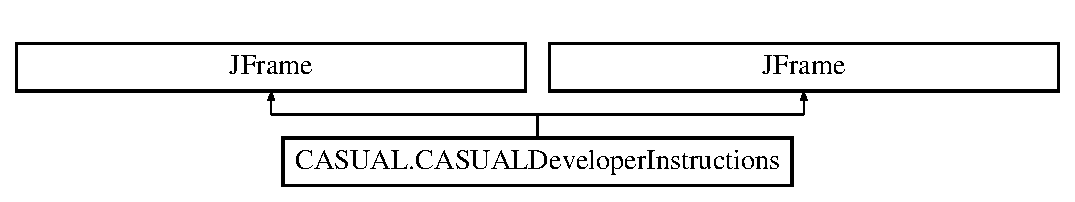
\includegraphics[height=2.000000cm]{classCASUAL_1_1CASUALDeveloperInstructions}
\end{center}
\end{figure}
\subsection*{Public Member Functions}
\begin{DoxyCompactItemize}
\item 
\hyperlink{classCASUAL_1_1CASUALDeveloperInstructions_a7ddef8688a60e51e7b1ce848d250287c}{C\-A\-S\-U\-A\-L\-Developer\-Instructions} ()
\item 
\hyperlink{classCASUAL_1_1CASUALDeveloperInstructions_a7ddef8688a60e51e7b1ce848d250287c}{C\-A\-S\-U\-A\-L\-Developer\-Instructions} ()
\end{DoxyCompactItemize}
\subsection*{Static Public Member Functions}
\begin{DoxyCompactItemize}
\item 
static void \hyperlink{classCASUAL_1_1CASUALDeveloperInstructions_a9fdc7d5a093dd16664125cd09de3da77}{main} ()
\item 
static void \hyperlink{classCASUAL_1_1CASUALDeveloperInstructions_a9fdc7d5a093dd16664125cd09de3da77}{main} ()
\end{DoxyCompactItemize}


\subsection{Detailed Description}
\begin{DoxyAuthor}{Author}
adam 
\end{DoxyAuthor}


\subsection{Constructor \& Destructor Documentation}
\hypertarget{classCASUAL_1_1CASUALDeveloperInstructions_a7ddef8688a60e51e7b1ce848d250287c}{\index{C\-A\-S\-U\-A\-L\-::\-C\-A\-S\-U\-A\-L\-Developer\-Instructions@{C\-A\-S\-U\-A\-L\-::\-C\-A\-S\-U\-A\-L\-Developer\-Instructions}!C\-A\-S\-U\-A\-L\-Developer\-Instructions@{C\-A\-S\-U\-A\-L\-Developer\-Instructions}}
\index{C\-A\-S\-U\-A\-L\-Developer\-Instructions@{C\-A\-S\-U\-A\-L\-Developer\-Instructions}!CASUAL::CASUALDeveloperInstructions@{C\-A\-S\-U\-A\-L\-::\-C\-A\-S\-U\-A\-L\-Developer\-Instructions}}
\subsubsection[{C\-A\-S\-U\-A\-L\-Developer\-Instructions}]{\setlength{\rightskip}{0pt plus 5cm}C\-A\-S\-U\-A\-L.\-C\-A\-S\-U\-A\-L\-Developer\-Instructions.\-C\-A\-S\-U\-A\-L\-Developer\-Instructions (
\begin{DoxyParamCaption}
{}
\end{DoxyParamCaption}
)}}\label{classCASUAL_1_1CASUALDeveloperInstructions_a7ddef8688a60e51e7b1ce848d250287c}
Creates new form \hyperlink{classCASUAL_1_1CASUALDeveloperInstructions}{C\-A\-S\-U\-A\-L\-Developer\-Instructions} \hypertarget{classCASUAL_1_1CASUALDeveloperInstructions_a7ddef8688a60e51e7b1ce848d250287c}{\index{C\-A\-S\-U\-A\-L\-::\-C\-A\-S\-U\-A\-L\-Developer\-Instructions@{C\-A\-S\-U\-A\-L\-::\-C\-A\-S\-U\-A\-L\-Developer\-Instructions}!C\-A\-S\-U\-A\-L\-Developer\-Instructions@{C\-A\-S\-U\-A\-L\-Developer\-Instructions}}
\index{C\-A\-S\-U\-A\-L\-Developer\-Instructions@{C\-A\-S\-U\-A\-L\-Developer\-Instructions}!CASUAL::CASUALDeveloperInstructions@{C\-A\-S\-U\-A\-L\-::\-C\-A\-S\-U\-A\-L\-Developer\-Instructions}}
\subsubsection[{C\-A\-S\-U\-A\-L\-Developer\-Instructions}]{\setlength{\rightskip}{0pt plus 5cm}C\-A\-S\-U\-A\-L.\-C\-A\-S\-U\-A\-L\-Developer\-Instructions.\-C\-A\-S\-U\-A\-L\-Developer\-Instructions (
\begin{DoxyParamCaption}
{}
\end{DoxyParamCaption}
)}}\label{classCASUAL_1_1CASUALDeveloperInstructions_a7ddef8688a60e51e7b1ce848d250287c}
Creates new form \hyperlink{classCASUAL_1_1CASUALDeveloperInstructions}{C\-A\-S\-U\-A\-L\-Developer\-Instructions} 

\subsection{Member Function Documentation}
\hypertarget{classCASUAL_1_1CASUALDeveloperInstructions_a9fdc7d5a093dd16664125cd09de3da77}{\index{C\-A\-S\-U\-A\-L\-::\-C\-A\-S\-U\-A\-L\-Developer\-Instructions@{C\-A\-S\-U\-A\-L\-::\-C\-A\-S\-U\-A\-L\-Developer\-Instructions}!main@{main}}
\index{main@{main}!CASUAL::CASUALDeveloperInstructions@{C\-A\-S\-U\-A\-L\-::\-C\-A\-S\-U\-A\-L\-Developer\-Instructions}}
\subsubsection[{main}]{\setlength{\rightskip}{0pt plus 5cm}static void C\-A\-S\-U\-A\-L.\-C\-A\-S\-U\-A\-L\-Developer\-Instructions.\-main (
\begin{DoxyParamCaption}
{}
\end{DoxyParamCaption}
)\hspace{0.3cm}{\ttfamily [static]}}}\label{classCASUAL_1_1CASUALDeveloperInstructions_a9fdc7d5a093dd16664125cd09de3da77}

\begin{DoxyParams}{Parameters}
{\em args} & the command line arguments \\
\hline
\end{DoxyParams}
\hypertarget{classCASUAL_1_1CASUALDeveloperInstructions_a9fdc7d5a093dd16664125cd09de3da77}{\index{C\-A\-S\-U\-A\-L\-::\-C\-A\-S\-U\-A\-L\-Developer\-Instructions@{C\-A\-S\-U\-A\-L\-::\-C\-A\-S\-U\-A\-L\-Developer\-Instructions}!main@{main}}
\index{main@{main}!CASUAL::CASUALDeveloperInstructions@{C\-A\-S\-U\-A\-L\-::\-C\-A\-S\-U\-A\-L\-Developer\-Instructions}}
\subsubsection[{main}]{\setlength{\rightskip}{0pt plus 5cm}static void C\-A\-S\-U\-A\-L.\-C\-A\-S\-U\-A\-L\-Developer\-Instructions.\-main (
\begin{DoxyParamCaption}
{}
\end{DoxyParamCaption}
)\hspace{0.3cm}{\ttfamily [static]}}}\label{classCASUAL_1_1CASUALDeveloperInstructions_a9fdc7d5a093dd16664125cd09de3da77}

\begin{DoxyParams}{Parameters}
{\em args} & the command line arguments \\
\hline
\end{DoxyParams}


The documentation for this class was generated from the following files\-:\begin{DoxyCompactItemize}
\item 
branches/\-C\-A\-S\-U\-A\-L-\/\-Headless/\-G\-U\-I/src/\-C\-A\-S\-U\-A\-L/C\-A\-S\-U\-A\-L\-Developer\-Instructions.\-java\item 
branches/\-Testing\-Branch/\-G\-Doc/src/\-C\-A\-S\-U\-A\-L/C\-A\-S\-U\-A\-L\-Developer\-Instructions.\-java\end{DoxyCompactItemize}

\hypertarget{classCASUAL_1_1network_1_1CASUALDevIntegration_1_1CASUALDevQuerier}{\section{C\-A\-S\-U\-A\-L.\-network.\-C\-A\-S\-U\-A\-L\-Dev\-Integration.\-C\-A\-S\-U\-A\-L\-Dev\-Querier Class Reference}
\label{classCASUAL_1_1network_1_1CASUALDevIntegration_1_1CASUALDevQuerier}\index{C\-A\-S\-U\-A\-L.\-network.\-C\-A\-S\-U\-A\-L\-Dev\-Integration.\-C\-A\-S\-U\-A\-L\-Dev\-Querier@{C\-A\-S\-U\-A\-L.\-network.\-C\-A\-S\-U\-A\-L\-Dev\-Integration.\-C\-A\-S\-U\-A\-L\-Dev\-Querier}}
}
\subsection*{Public Member Functions}
\begin{DoxyCompactItemize}
\item 
\hyperlink{classCASUAL_1_1network_1_1CASUALDevIntegration_1_1CASUALDevQuerier_a851f08561077481b8e936ec4f2d08a23}{C\-A\-S\-U\-A\-L\-Dev\-Querier} (String device\-Build\-Prop, String\mbox{[}$\,$\mbox{]} additional\-Props)
\item 
String\mbox{[}$\,$\mbox{]} \hyperlink{classCASUAL_1_1network_1_1CASUALDevIntegration_1_1CASUALDevQuerier_aee336d5bb7286f639b6951d2552106d1}{recursive\-Folder\-Search} ()
\end{DoxyCompactItemize}


\subsection{Detailed Description}
\begin{DoxyAuthor}{Author}
adam 
\end{DoxyAuthor}


\subsection{Constructor \& Destructor Documentation}
\hypertarget{classCASUAL_1_1network_1_1CASUALDevIntegration_1_1CASUALDevQuerier_a851f08561077481b8e936ec4f2d08a23}{\index{C\-A\-S\-U\-A\-L\-::network\-::\-C\-A\-S\-U\-A\-L\-Dev\-Integration\-::\-C\-A\-S\-U\-A\-L\-Dev\-Querier@{C\-A\-S\-U\-A\-L\-::network\-::\-C\-A\-S\-U\-A\-L\-Dev\-Integration\-::\-C\-A\-S\-U\-A\-L\-Dev\-Querier}!C\-A\-S\-U\-A\-L\-Dev\-Querier@{C\-A\-S\-U\-A\-L\-Dev\-Querier}}
\index{C\-A\-S\-U\-A\-L\-Dev\-Querier@{C\-A\-S\-U\-A\-L\-Dev\-Querier}!CASUAL::network::CASUALDevIntegration::CASUALDevQuerier@{C\-A\-S\-U\-A\-L\-::network\-::\-C\-A\-S\-U\-A\-L\-Dev\-Integration\-::\-C\-A\-S\-U\-A\-L\-Dev\-Querier}}
\subsubsection[{C\-A\-S\-U\-A\-L\-Dev\-Querier}]{\setlength{\rightskip}{0pt plus 5cm}C\-A\-S\-U\-A\-L.\-network.\-C\-A\-S\-U\-A\-L\-Dev\-Integration.\-C\-A\-S\-U\-A\-L\-Dev\-Querier.\-C\-A\-S\-U\-A\-L\-Dev\-Querier (
\begin{DoxyParamCaption}
\item[{String}]{device\-Build\-Prop, }
\item[{String\mbox{[}$\,$\mbox{]}}]{additional\-Props}
\end{DoxyParamCaption}
)}}\label{classCASUAL_1_1network_1_1CASUALDevIntegration_1_1CASUALDevQuerier_a851f08561077481b8e936ec4f2d08a23}
Takes the build.\-prop and instantiates Casual\-Dev\-Querier


\begin{DoxyParams}{Parameters}
{\em device\-Build\-Prop} & from an android device. \\
\hline
{\em additional\-Props} & additional properties to blacklist \\
\hline
\end{DoxyParams}


\subsection{Member Function Documentation}
\hypertarget{classCASUAL_1_1network_1_1CASUALDevIntegration_1_1CASUALDevQuerier_aee336d5bb7286f639b6951d2552106d1}{\index{C\-A\-S\-U\-A\-L\-::network\-::\-C\-A\-S\-U\-A\-L\-Dev\-Integration\-::\-C\-A\-S\-U\-A\-L\-Dev\-Querier@{C\-A\-S\-U\-A\-L\-::network\-::\-C\-A\-S\-U\-A\-L\-Dev\-Integration\-::\-C\-A\-S\-U\-A\-L\-Dev\-Querier}!recursive\-Folder\-Search@{recursive\-Folder\-Search}}
\index{recursive\-Folder\-Search@{recursive\-Folder\-Search}!CASUAL::network::CASUALDevIntegration::CASUALDevQuerier@{C\-A\-S\-U\-A\-L\-::network\-::\-C\-A\-S\-U\-A\-L\-Dev\-Integration\-::\-C\-A\-S\-U\-A\-L\-Dev\-Querier}}
\subsubsection[{recursive\-Folder\-Search}]{\setlength{\rightskip}{0pt plus 5cm}String \mbox{[}$\,$\mbox{]} C\-A\-S\-U\-A\-L.\-network.\-C\-A\-S\-U\-A\-L\-Dev\-Integration.\-C\-A\-S\-U\-A\-L\-Dev\-Querier.\-recursive\-Folder\-Search (
\begin{DoxyParamCaption}
{}
\end{DoxyParamCaption}
)}}\label{classCASUAL_1_1network_1_1CASUALDevIntegration_1_1CASUALDevQuerier_aee336d5bb7286f639b6951d2552106d1}
Performs a recursive search of builds.\-casual-\/dev.\-com \begin{DoxyReturn}{Returns}
an array of U\-R\-Ls in string format representing available files. 
\end{DoxyReturn}


The documentation for this class was generated from the following file\-:\begin{DoxyCompactItemize}
\item 
trunk/\-C\-A\-S\-U\-A\-Lcore/src/\-C\-A\-S\-U\-A\-L/network/\-C\-A\-S\-U\-A\-L\-Dev\-Integration/C\-A\-S\-U\-A\-L\-Dev\-Querier.\-java\end{DoxyCompactItemize}

\hypertarget{classCASUAL_1_1network_1_1CASUALDevIntegration_1_1CASUALDevQuerierTest}{\section{C\-A\-S\-U\-A\-L.\-network.\-C\-A\-S\-U\-A\-L\-Dev\-Integration.\-C\-A\-S\-U\-A\-L\-Dev\-Querier\-Test Class Reference}
\label{classCASUAL_1_1network_1_1CASUALDevIntegration_1_1CASUALDevQuerierTest}\index{C\-A\-S\-U\-A\-L.\-network.\-C\-A\-S\-U\-A\-L\-Dev\-Integration.\-C\-A\-S\-U\-A\-L\-Dev\-Querier\-Test@{C\-A\-S\-U\-A\-L.\-network.\-C\-A\-S\-U\-A\-L\-Dev\-Integration.\-C\-A\-S\-U\-A\-L\-Dev\-Querier\-Test}}
}
\subsection*{Public Member Functions}
\begin{DoxyCompactItemize}
\item 
\hypertarget{classCASUAL_1_1network_1_1CASUALDevIntegration_1_1CASUALDevQuerierTest_ac8e09bd2ab2c941c1080d98ee0c48c4b}{void {\bfseries set\-Up} ()}\label{classCASUAL_1_1network_1_1CASUALDevIntegration_1_1CASUALDevQuerierTest_ac8e09bd2ab2c941c1080d98ee0c48c4b}

\item 
\hypertarget{classCASUAL_1_1network_1_1CASUALDevIntegration_1_1CASUALDevQuerierTest_a6f30be752510a1b442aeef6dd77a9f8f}{void {\bfseries tear\-Down} ()}\label{classCASUAL_1_1network_1_1CASUALDevIntegration_1_1CASUALDevQuerierTest_a6f30be752510a1b442aeef6dd77a9f8f}

\item 
\hypertarget{classCASUAL_1_1network_1_1CASUALDevIntegration_1_1CASUALDevQuerierTest_a52313b3c6c7b628d081efa139e3c5d61}{void {\bfseries test\-Do\-Property\-Search} ()  throws Exception }\label{classCASUAL_1_1network_1_1CASUALDevIntegration_1_1CASUALDevQuerierTest_a52313b3c6c7b628d081efa139e3c5d61}

\end{DoxyCompactItemize}


\subsection{Detailed Description}
\begin{DoxyAuthor}{Author}
adam 
\end{DoxyAuthor}


The documentation for this class was generated from the following file\-:\begin{DoxyCompactItemize}
\item 
trunk/\-C\-A\-S\-U\-A\-Lcore/test/\-C\-A\-S\-U\-A\-L/network/\-C\-A\-S\-U\-A\-L\-Dev\-Integration/C\-A\-S\-U\-A\-L\-Dev\-Querier\-Test.\-java\end{DoxyCompactItemize}

\hypertarget{classCASUAL_1_1gDrive_1_1CASUALGDrive}{\section{C\-A\-S\-U\-A\-L.\-g\-Drive.\-C\-A\-S\-U\-A\-L\-G\-Drive Class Reference}
\label{classCASUAL_1_1gDrive_1_1CASUALGDrive}\index{C\-A\-S\-U\-A\-L.\-g\-Drive.\-C\-A\-S\-U\-A\-L\-G\-Drive@{C\-A\-S\-U\-A\-L.\-g\-Drive.\-C\-A\-S\-U\-A\-L\-G\-Drive}}
}
\subsection*{Static Public Member Functions}
\begin{DoxyCompactItemize}
\item 
static Credential \hyperlink{classCASUAL_1_1gDrive_1_1CASUALGDrive_ab0165abaa127f7c5d85be97ecabbb383}{authorize} ()  throws Exception 
\item 
\hypertarget{classCASUAL_1_1gDrive_1_1CASUALGDrive_a6efc668bbf4bb5138006248cbe98a3c1}{static void {\bfseries main} (String\mbox{[}$\,$\mbox{]} args)}\label{classCASUAL_1_1gDrive_1_1CASUALGDrive_a6efc668bbf4bb5138006248cbe98a3c1}

\item 
static File \hyperlink{classCASUAL_1_1gDrive_1_1CASUALGDrive_a1da14b5175423bd7fe54003577ee7462}{upload\-File} (boolean use\-Direct\-Upload, java.\-io.\-File upload\-File)  throws I\-O\-Exception 
\item 
\hypertarget{classCASUAL_1_1gDrive_1_1CASUALGDrive_ab303c515c64dc4929186b85e8daaf271}{static List$<$ File $>$ {\bfseries get\-All\-Files\-From\-Drive} ()  throws I\-O\-Exception     }\label{classCASUAL_1_1gDrive_1_1CASUALGDrive_ab303c515c64dc4929186b85e8daaf271}

\item 
\hypertarget{classCASUAL_1_1gDrive_1_1CASUALGDrive_ae8429a953c5ba0c50e26d6770ce45908}{static List$<$ String $>$ {\bfseries get\-All\-File\-Names} ()  throws I\-O\-Exception }\label{classCASUAL_1_1gDrive_1_1CASUALGDrive_ae8429a953c5ba0c50e26d6770ce45908}

\item 
\hypertarget{classCASUAL_1_1gDrive_1_1CASUALGDrive_a4761af4b083cec83c9719f8bc8fbfd7c}{static File {\bfseries get\-File\-Query} (String query)  throws I\-O\-Exception       }\label{classCASUAL_1_1gDrive_1_1CASUALGDrive_a4761af4b083cec83c9719f8bc8fbfd7c}

\item 
static File \hyperlink{classCASUAL_1_1gDrive_1_1CASUALGDrive_ac88c1b89f50ee1045540d33ff3e8bf1d}{update\-File\-With\-Test\-Suffix} (String id, java.\-io.\-File file)  throws I\-O\-Exception 
\item 
static void \hyperlink{classCASUAL_1_1gDrive_1_1CASUALGDrive_af88eb897e7c2f6011f5ac2ed061b1a2c}{download\-File} (boolean use\-Direct\-Download, File download\-File, String file\-Loc)  throws I\-O\-Exception 
\end{DoxyCompactItemize}
\subsection*{Static Public Attributes}
\begin{DoxyCompactItemize}
\item 
static Drive \hyperlink{classCASUAL_1_1gDrive_1_1CASUALGDrive_ae4c31951e931fb6eeafc818873646451}{drive}
\end{DoxyCompactItemize}


\subsection{Detailed Description}
\begin{DoxyAuthor}{Author}
loglud 
\end{DoxyAuthor}


\subsection{Member Function Documentation}
\hypertarget{classCASUAL_1_1gDrive_1_1CASUALGDrive_ab0165abaa127f7c5d85be97ecabbb383}{\index{C\-A\-S\-U\-A\-L\-::g\-Drive\-::\-C\-A\-S\-U\-A\-L\-G\-Drive@{C\-A\-S\-U\-A\-L\-::g\-Drive\-::\-C\-A\-S\-U\-A\-L\-G\-Drive}!authorize@{authorize}}
\index{authorize@{authorize}!CASUAL::gDrive::CASUALGDrive@{C\-A\-S\-U\-A\-L\-::g\-Drive\-::\-C\-A\-S\-U\-A\-L\-G\-Drive}}
\subsubsection[{authorize}]{\setlength{\rightskip}{0pt plus 5cm}static Credential C\-A\-S\-U\-A\-L.\-g\-Drive.\-C\-A\-S\-U\-A\-L\-G\-Drive.\-authorize (
\begin{DoxyParamCaption}
{}
\end{DoxyParamCaption}
) throws Exception\hspace{0.3cm}{\ttfamily [static]}}}\label{classCASUAL_1_1gDrive_1_1CASUALGDrive_ab0165abaa127f7c5d85be97ecabbb383}
Authorizes the installed application to access user's protected data. \hypertarget{classCASUAL_1_1gDrive_1_1CASUALGDrive_af88eb897e7c2f6011f5ac2ed061b1a2c}{\index{C\-A\-S\-U\-A\-L\-::g\-Drive\-::\-C\-A\-S\-U\-A\-L\-G\-Drive@{C\-A\-S\-U\-A\-L\-::g\-Drive\-::\-C\-A\-S\-U\-A\-L\-G\-Drive}!download\-File@{download\-File}}
\index{download\-File@{download\-File}!CASUAL::gDrive::CASUALGDrive@{C\-A\-S\-U\-A\-L\-::g\-Drive\-::\-C\-A\-S\-U\-A\-L\-G\-Drive}}
\subsubsection[{download\-File}]{\setlength{\rightskip}{0pt plus 5cm}static void C\-A\-S\-U\-A\-L.\-g\-Drive.\-C\-A\-S\-U\-A\-L\-G\-Drive.\-download\-File (
\begin{DoxyParamCaption}
\item[{boolean}]{use\-Direct\-Download, }
\item[{File}]{download\-File, }
\item[{String}]{file\-Loc}
\end{DoxyParamCaption}
) throws I\-O\-Exception\hspace{0.3cm}{\ttfamily [static]}}}\label{classCASUAL_1_1gDrive_1_1CASUALGDrive_af88eb897e7c2f6011f5ac2ed061b1a2c}
Downloads a file using either resumable or direct media download. \hypertarget{classCASUAL_1_1gDrive_1_1CASUALGDrive_ac88c1b89f50ee1045540d33ff3e8bf1d}{\index{C\-A\-S\-U\-A\-L\-::g\-Drive\-::\-C\-A\-S\-U\-A\-L\-G\-Drive@{C\-A\-S\-U\-A\-L\-::g\-Drive\-::\-C\-A\-S\-U\-A\-L\-G\-Drive}!update\-File\-With\-Test\-Suffix@{update\-File\-With\-Test\-Suffix}}
\index{update\-File\-With\-Test\-Suffix@{update\-File\-With\-Test\-Suffix}!CASUAL::gDrive::CASUALGDrive@{C\-A\-S\-U\-A\-L\-::g\-Drive\-::\-C\-A\-S\-U\-A\-L\-G\-Drive}}
\subsubsection[{update\-File\-With\-Test\-Suffix}]{\setlength{\rightskip}{0pt plus 5cm}static File C\-A\-S\-U\-A\-L.\-g\-Drive.\-C\-A\-S\-U\-A\-L\-G\-Drive.\-update\-File\-With\-Test\-Suffix (
\begin{DoxyParamCaption}
\item[{String}]{id, }
\item[{java.\-io.\-File}]{file}
\end{DoxyParamCaption}
) throws I\-O\-Exception\hspace{0.3cm}{\ttfamily [static]}}}\label{classCASUAL_1_1gDrive_1_1CASUALGDrive_ac88c1b89f50ee1045540d33ff3e8bf1d}
Updates the name of the uploaded file to have a \char`\"{}drivetest-\/\char`\"{} prefix. \hypertarget{classCASUAL_1_1gDrive_1_1CASUALGDrive_a1da14b5175423bd7fe54003577ee7462}{\index{C\-A\-S\-U\-A\-L\-::g\-Drive\-::\-C\-A\-S\-U\-A\-L\-G\-Drive@{C\-A\-S\-U\-A\-L\-::g\-Drive\-::\-C\-A\-S\-U\-A\-L\-G\-Drive}!upload\-File@{upload\-File}}
\index{upload\-File@{upload\-File}!CASUAL::gDrive::CASUALGDrive@{C\-A\-S\-U\-A\-L\-::g\-Drive\-::\-C\-A\-S\-U\-A\-L\-G\-Drive}}
\subsubsection[{upload\-File}]{\setlength{\rightskip}{0pt plus 5cm}static File C\-A\-S\-U\-A\-L.\-g\-Drive.\-C\-A\-S\-U\-A\-L\-G\-Drive.\-upload\-File (
\begin{DoxyParamCaption}
\item[{boolean}]{use\-Direct\-Upload, }
\item[{java.\-io.\-File}]{upload\-File}
\end{DoxyParamCaption}
) throws I\-O\-Exception\hspace{0.3cm}{\ttfamily [static]}}}\label{classCASUAL_1_1gDrive_1_1CASUALGDrive_a1da14b5175423bd7fe54003577ee7462}
Uploads a file using either resumable or direct media upload. 

\subsection{Member Data Documentation}
\hypertarget{classCASUAL_1_1gDrive_1_1CASUALGDrive_ae4c31951e931fb6eeafc818873646451}{\index{C\-A\-S\-U\-A\-L\-::g\-Drive\-::\-C\-A\-S\-U\-A\-L\-G\-Drive@{C\-A\-S\-U\-A\-L\-::g\-Drive\-::\-C\-A\-S\-U\-A\-L\-G\-Drive}!drive@{drive}}
\index{drive@{drive}!CASUAL::gDrive::CASUALGDrive@{C\-A\-S\-U\-A\-L\-::g\-Drive\-::\-C\-A\-S\-U\-A\-L\-G\-Drive}}
\subsubsection[{drive}]{\setlength{\rightskip}{0pt plus 5cm}Drive C\-A\-S\-U\-A\-L.\-g\-Drive.\-C\-A\-S\-U\-A\-L\-G\-Drive.\-drive\hspace{0.3cm}{\ttfamily [static]}}}\label{classCASUAL_1_1gDrive_1_1CASUALGDrive_ae4c31951e931fb6eeafc818873646451}
Global Drive A\-P\-I client. 

The documentation for this class was generated from the following file\-:\begin{DoxyCompactItemize}
\item 
branches/\-Testing\-Branch/\-G\-Doc/src/\-C\-A\-S\-U\-A\-L/g\-Drive/C\-A\-S\-U\-A\-L\-G\-Drive.\-java\end{DoxyCompactItemize}

\hypertarget{classCASUAL_1_1CASUALInteractionsjUnitTest}{\section{C\-A\-S\-U\-A\-L.\-C\-A\-S\-U\-A\-L\-Interactionsj\-Unit\-Test Class Reference}
\label{classCASUAL_1_1CASUALInteractionsjUnitTest}\index{C\-A\-S\-U\-A\-L.\-C\-A\-S\-U\-A\-L\-Interactionsj\-Unit\-Test@{C\-A\-S\-U\-A\-L.\-C\-A\-S\-U\-A\-L\-Interactionsj\-Unit\-Test}}
}
\subsection*{Public Member Functions}
\begin{DoxyCompactItemize}
\item 
\hypertarget{classCASUAL_1_1CASUALInteractionsjUnitTest_a64a391116813aa0f8bd3d5e11335887a}{void {\bfseries test\-C\-A\-S\-U\-A\-L\-Interactions} ()}\label{classCASUAL_1_1CASUALInteractionsjUnitTest_a64a391116813aa0f8bd3d5e11335887a}

\end{DoxyCompactItemize}
\subsection*{Static Public Member Functions}
\begin{DoxyCompactItemize}
\item 
\hypertarget{classCASUAL_1_1CASUALInteractionsjUnitTest_a923fdc5c9d81cefa1a91638926c4e5c6}{static void {\bfseries set\-Up\-Class} ()}\label{classCASUAL_1_1CASUALInteractionsjUnitTest_a923fdc5c9d81cefa1a91638926c4e5c6}

\item 
\hypertarget{classCASUAL_1_1CASUALInteractionsjUnitTest_a4b1cb544659fec5aebb74dae55c72452}{static void {\bfseries tear\-Down\-Class} ()}\label{classCASUAL_1_1CASUALInteractionsjUnitTest_a4b1cb544659fec5aebb74dae55c72452}

\end{DoxyCompactItemize}


\subsection{Detailed Description}
\begin{DoxyAuthor}{Author}
adam 
\end{DoxyAuthor}


The documentation for this class was generated from the following file\-:\begin{DoxyCompactItemize}
\item 
trunk/\-C\-A\-S\-U\-A\-Lcore/test/\-C\-A\-S\-U\-A\-L/C\-A\-S\-U\-A\-L\-Interactionsj\-Unit\-Test.\-java\end{DoxyCompactItemize}

\hypertarget{classCASUAL_1_1CASUALJFrame}{\section{C\-A\-S\-U\-A\-L.\-C\-A\-S\-U\-A\-L\-J\-Frame Class Reference}
\label{classCASUAL_1_1CASUALJFrame}\index{C\-A\-S\-U\-A\-L.\-C\-A\-S\-U\-A\-L\-J\-Frame@{C\-A\-S\-U\-A\-L.\-C\-A\-S\-U\-A\-L\-J\-Frame}}
}
Inheritance diagram for C\-A\-S\-U\-A\-L.\-C\-A\-S\-U\-A\-L\-J\-Frame\-:\begin{figure}[H]
\begin{center}
\leavevmode
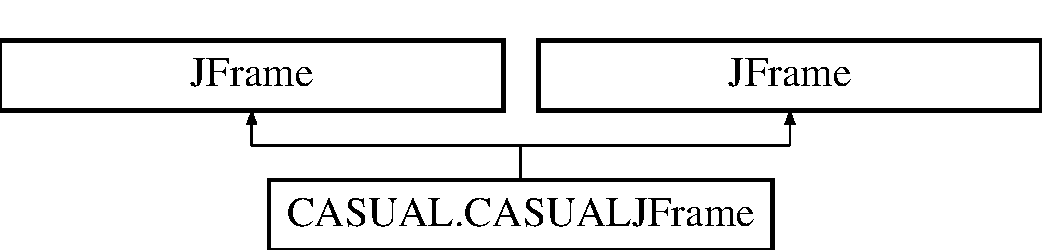
\includegraphics[height=2.000000cm]{classCASUAL_1_1CASUALJFrame}
\end{center}
\end{figure}
\subsection*{Public Member Functions}
\begin{DoxyCompactItemize}
\item 
\hyperlink{classCASUAL_1_1CASUALJFrame_a75bc21e996105a528667cd5866789df6}{C\-A\-S\-U\-A\-L\-J\-Frame} ()
\item 
\hypertarget{classCASUAL_1_1CASUALJFrame_ab8c6685f91aed222205e96fbfe5f4e4a}{void {\bfseries set\-Status\-Label\-Icon} (String Icon, String Text)}\label{classCASUAL_1_1CASUALJFrame_ab8c6685f91aed222205e96fbfe5f4e4a}

\item 
\hypertarget{classCASUAL_1_1CASUALJFrame_a6df28504e65c9a926b89894d730a3e65}{void {\bfseries start\-Stop\-Timer} (boolean State\-Commanded)}\label{classCASUAL_1_1CASUALJFrame_a6df28504e65c9a926b89894d730a3e65}

\item 
\hypertarget{classCASUAL_1_1CASUALJFrame_a274d90b3b9a8d3e126896b6c0c356139}{void {\bfseries set\-Status\-Message\-Label} (String text)}\label{classCASUAL_1_1CASUALJFrame_a274d90b3b9a8d3e126896b6c0c356139}

\item 
\hypertarget{classCASUAL_1_1CASUALJFrame_a60805d1440958d7811bf18c921274695}{void {\bfseries enable\-Controls} (boolean status)}\label{classCASUAL_1_1CASUALJFrame_a60805d1440958d7811bf18c921274695}

\item 
\hyperlink{classCASUAL_1_1CASUALJFrame_a75bc21e996105a528667cd5866789df6}{C\-A\-S\-U\-A\-L\-J\-Frame} ()
\item 
\hypertarget{classCASUAL_1_1CASUALJFrame_ab8c6685f91aed222205e96fbfe5f4e4a}{void {\bfseries set\-Status\-Label\-Icon} (String Icon, String Text)}\label{classCASUAL_1_1CASUALJFrame_ab8c6685f91aed222205e96fbfe5f4e4a}

\item 
\hypertarget{classCASUAL_1_1CASUALJFrame_a6df28504e65c9a926b89894d730a3e65}{void {\bfseries start\-Stop\-Timer} (boolean State\-Commanded)}\label{classCASUAL_1_1CASUALJFrame_a6df28504e65c9a926b89894d730a3e65}

\item 
\hypertarget{classCASUAL_1_1CASUALJFrame_a274d90b3b9a8d3e126896b6c0c356139}{void {\bfseries set\-Status\-Message\-Label} (String text)}\label{classCASUAL_1_1CASUALJFrame_a274d90b3b9a8d3e126896b6c0c356139}

\item 
\hypertarget{classCASUAL_1_1CASUALJFrame_a60805d1440958d7811bf18c921274695}{void {\bfseries enable\-Controls} (boolean status)}\label{classCASUAL_1_1CASUALJFrame_a60805d1440958d7811bf18c921274695}

\end{DoxyCompactItemize}
\subsection*{Protected Member Functions}
\begin{DoxyCompactItemize}
\item 
\hypertarget{classCASUAL_1_1CASUALJFrame_a980c3bf8b6a3d1c65f9ca5ecac0220b9}{Image\-Icon {\bfseries create\-Image\-Icon} (String path, String description)}\label{classCASUAL_1_1CASUALJFrame_a980c3bf8b6a3d1c65f9ca5ecac0220b9}

\item 
\hypertarget{classCASUAL_1_1CASUALJFrame_a980c3bf8b6a3d1c65f9ca5ecac0220b9}{Image\-Icon {\bfseries create\-Image\-Icon} (String path, String description)}\label{classCASUAL_1_1CASUALJFrame_a980c3bf8b6a3d1c65f9ca5ecac0220b9}

\end{DoxyCompactItemize}


\subsection{Detailed Description}
\begin{DoxyAuthor}{Author}
adam 
\end{DoxyAuthor}


\subsection{Constructor \& Destructor Documentation}
\hypertarget{classCASUAL_1_1CASUALJFrame_a75bc21e996105a528667cd5866789df6}{\index{C\-A\-S\-U\-A\-L\-::\-C\-A\-S\-U\-A\-L\-J\-Frame@{C\-A\-S\-U\-A\-L\-::\-C\-A\-S\-U\-A\-L\-J\-Frame}!C\-A\-S\-U\-A\-L\-J\-Frame@{C\-A\-S\-U\-A\-L\-J\-Frame}}
\index{C\-A\-S\-U\-A\-L\-J\-Frame@{C\-A\-S\-U\-A\-L\-J\-Frame}!CASUAL::CASUALJFrame@{C\-A\-S\-U\-A\-L\-::\-C\-A\-S\-U\-A\-L\-J\-Frame}}
\subsubsection[{C\-A\-S\-U\-A\-L\-J\-Frame}]{\setlength{\rightskip}{0pt plus 5cm}C\-A\-S\-U\-A\-L.\-C\-A\-S\-U\-A\-L\-J\-Frame.\-C\-A\-S\-U\-A\-L\-J\-Frame (
\begin{DoxyParamCaption}
{}
\end{DoxyParamCaption}
)}}\label{classCASUAL_1_1CASUALJFrame_a75bc21e996105a528667cd5866789df6}
Creates new form C\-A\-S\-U\-A\-L\-J\-Frame2 \hypertarget{classCASUAL_1_1CASUALJFrame_a75bc21e996105a528667cd5866789df6}{\index{C\-A\-S\-U\-A\-L\-::\-C\-A\-S\-U\-A\-L\-J\-Frame@{C\-A\-S\-U\-A\-L\-::\-C\-A\-S\-U\-A\-L\-J\-Frame}!C\-A\-S\-U\-A\-L\-J\-Frame@{C\-A\-S\-U\-A\-L\-J\-Frame}}
\index{C\-A\-S\-U\-A\-L\-J\-Frame@{C\-A\-S\-U\-A\-L\-J\-Frame}!CASUAL::CASUALJFrame@{C\-A\-S\-U\-A\-L\-::\-C\-A\-S\-U\-A\-L\-J\-Frame}}
\subsubsection[{C\-A\-S\-U\-A\-L\-J\-Frame}]{\setlength{\rightskip}{0pt plus 5cm}C\-A\-S\-U\-A\-L.\-C\-A\-S\-U\-A\-L\-J\-Frame.\-C\-A\-S\-U\-A\-L\-J\-Frame (
\begin{DoxyParamCaption}
{}
\end{DoxyParamCaption}
)}}\label{classCASUAL_1_1CASUALJFrame_a75bc21e996105a528667cd5866789df6}
Creates new form C\-A\-S\-U\-A\-L\-J\-Frame2 

The documentation for this class was generated from the following files\-:\begin{DoxyCompactItemize}
\item 
branches/\-C\-A\-S\-U\-A\-L-\/\-Headless/\-G\-U\-I/src/\-C\-A\-S\-U\-A\-L/C\-A\-S\-U\-A\-L\-J\-Frame.\-java\item 
branches/\-Testing\-Branch/\-G\-Doc/src/\-C\-A\-S\-U\-A\-L/C\-A\-S\-U\-A\-L\-J\-Frame.\-java\end{DoxyCompactItemize}

\hypertarget{classGUI_1_1development_1_1CASUALJFrameAboutBox}{\section{G\-U\-I.\-development.\-C\-A\-S\-U\-A\-L\-J\-Frame\-About\-Box Class Reference}
\label{classGUI_1_1development_1_1CASUALJFrameAboutBox}\index{G\-U\-I.\-development.\-C\-A\-S\-U\-A\-L\-J\-Frame\-About\-Box@{G\-U\-I.\-development.\-C\-A\-S\-U\-A\-L\-J\-Frame\-About\-Box}}
}
Inheritance diagram for G\-U\-I.\-development.\-C\-A\-S\-U\-A\-L\-J\-Frame\-About\-Box\-:\begin{figure}[H]
\begin{center}
\leavevmode
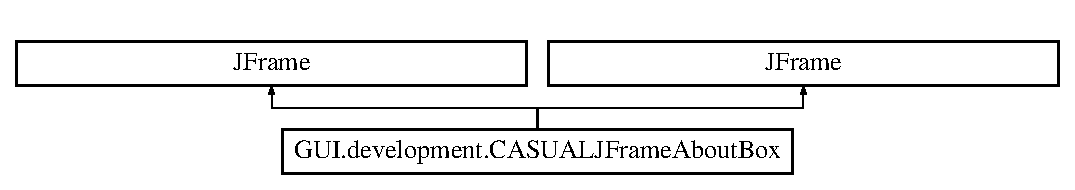
\includegraphics[height=2.000000cm]{classGUI_1_1development_1_1CASUALJFrameAboutBox}
\end{center}
\end{figure}
\subsection*{Public Member Functions}
\begin{DoxyCompactItemize}
\item 
\hyperlink{classGUI_1_1development_1_1CASUALJFrameAboutBox_a8323c1fa354fb8f2ecdaf5e373c77423}{C\-A\-S\-U\-A\-L\-J\-Frame\-About\-Box} ()
\item 
\hyperlink{classGUI_1_1development_1_1CASUALJFrameAboutBox_a8323c1fa354fb8f2ecdaf5e373c77423}{C\-A\-S\-U\-A\-L\-J\-Frame\-About\-Box} ()
\end{DoxyCompactItemize}
\subsection*{Static Public Member Functions}
\begin{DoxyCompactItemize}
\item 
static void \hyperlink{classGUI_1_1development_1_1CASUALJFrameAboutBox_ab86c75e03d79f695e1b26b10037f63bc}{main} ()
\item 
static void \hyperlink{classGUI_1_1development_1_1CASUALJFrameAboutBox_ab86c75e03d79f695e1b26b10037f63bc}{main} ()
\end{DoxyCompactItemize}


\subsection{Detailed Description}
\begin{DoxyAuthor}{Author}
adam 
\end{DoxyAuthor}


\subsection{Constructor \& Destructor Documentation}
\hypertarget{classGUI_1_1development_1_1CASUALJFrameAboutBox_a8323c1fa354fb8f2ecdaf5e373c77423}{\index{G\-U\-I\-::development\-::\-C\-A\-S\-U\-A\-L\-J\-Frame\-About\-Box@{G\-U\-I\-::development\-::\-C\-A\-S\-U\-A\-L\-J\-Frame\-About\-Box}!C\-A\-S\-U\-A\-L\-J\-Frame\-About\-Box@{C\-A\-S\-U\-A\-L\-J\-Frame\-About\-Box}}
\index{C\-A\-S\-U\-A\-L\-J\-Frame\-About\-Box@{C\-A\-S\-U\-A\-L\-J\-Frame\-About\-Box}!GUI::development::CASUALJFrameAboutBox@{G\-U\-I\-::development\-::\-C\-A\-S\-U\-A\-L\-J\-Frame\-About\-Box}}
\subsubsection[{C\-A\-S\-U\-A\-L\-J\-Frame\-About\-Box}]{\setlength{\rightskip}{0pt plus 5cm}G\-U\-I.\-development.\-C\-A\-S\-U\-A\-L\-J\-Frame\-About\-Box.\-C\-A\-S\-U\-A\-L\-J\-Frame\-About\-Box (
\begin{DoxyParamCaption}
{}
\end{DoxyParamCaption}
)}}\label{classGUI_1_1development_1_1CASUALJFrameAboutBox_a8323c1fa354fb8f2ecdaf5e373c77423}
Creates new form C\-A\-S\-U\-A\-L\-About\-Box1 \hypertarget{classGUI_1_1development_1_1CASUALJFrameAboutBox_a8323c1fa354fb8f2ecdaf5e373c77423}{\index{G\-U\-I\-::development\-::\-C\-A\-S\-U\-A\-L\-J\-Frame\-About\-Box@{G\-U\-I\-::development\-::\-C\-A\-S\-U\-A\-L\-J\-Frame\-About\-Box}!C\-A\-S\-U\-A\-L\-J\-Frame\-About\-Box@{C\-A\-S\-U\-A\-L\-J\-Frame\-About\-Box}}
\index{C\-A\-S\-U\-A\-L\-J\-Frame\-About\-Box@{C\-A\-S\-U\-A\-L\-J\-Frame\-About\-Box}!GUI::development::CASUALJFrameAboutBox@{G\-U\-I\-::development\-::\-C\-A\-S\-U\-A\-L\-J\-Frame\-About\-Box}}
\subsubsection[{C\-A\-S\-U\-A\-L\-J\-Frame\-About\-Box}]{\setlength{\rightskip}{0pt plus 5cm}G\-U\-I.\-development.\-C\-A\-S\-U\-A\-L\-J\-Frame\-About\-Box.\-C\-A\-S\-U\-A\-L\-J\-Frame\-About\-Box (
\begin{DoxyParamCaption}
{}
\end{DoxyParamCaption}
)}}\label{classGUI_1_1development_1_1CASUALJFrameAboutBox_a8323c1fa354fb8f2ecdaf5e373c77423}
Creates new form C\-A\-S\-U\-A\-L\-About\-Box1 

\subsection{Member Function Documentation}
\hypertarget{classGUI_1_1development_1_1CASUALJFrameAboutBox_ab86c75e03d79f695e1b26b10037f63bc}{\index{G\-U\-I\-::development\-::\-C\-A\-S\-U\-A\-L\-J\-Frame\-About\-Box@{G\-U\-I\-::development\-::\-C\-A\-S\-U\-A\-L\-J\-Frame\-About\-Box}!main@{main}}
\index{main@{main}!GUI::development::CASUALJFrameAboutBox@{G\-U\-I\-::development\-::\-C\-A\-S\-U\-A\-L\-J\-Frame\-About\-Box}}
\subsubsection[{main}]{\setlength{\rightskip}{0pt plus 5cm}static void G\-U\-I.\-development.\-C\-A\-S\-U\-A\-L\-J\-Frame\-About\-Box.\-main (
\begin{DoxyParamCaption}
{}
\end{DoxyParamCaption}
)\hspace{0.3cm}{\ttfamily [static]}}}\label{classGUI_1_1development_1_1CASUALJFrameAboutBox_ab86c75e03d79f695e1b26b10037f63bc}
starts the about box \hypertarget{classGUI_1_1development_1_1CASUALJFrameAboutBox_ab86c75e03d79f695e1b26b10037f63bc}{\index{G\-U\-I\-::development\-::\-C\-A\-S\-U\-A\-L\-J\-Frame\-About\-Box@{G\-U\-I\-::development\-::\-C\-A\-S\-U\-A\-L\-J\-Frame\-About\-Box}!main@{main}}
\index{main@{main}!GUI::development::CASUALJFrameAboutBox@{G\-U\-I\-::development\-::\-C\-A\-S\-U\-A\-L\-J\-Frame\-About\-Box}}
\subsubsection[{main}]{\setlength{\rightskip}{0pt plus 5cm}static void G\-U\-I.\-development.\-C\-A\-S\-U\-A\-L\-J\-Frame\-About\-Box.\-main (
\begin{DoxyParamCaption}
{}
\end{DoxyParamCaption}
)\hspace{0.3cm}{\ttfamily [static]}}}\label{classGUI_1_1development_1_1CASUALJFrameAboutBox_ab86c75e03d79f695e1b26b10037f63bc}
starts the about box 

The documentation for this class was generated from the following files\-:\begin{DoxyCompactItemize}
\item 
trunk/\-C\-A\-S\-U\-A\-Lcore/build/classes/\-G\-U\-I/development/C\-A\-S\-U\-A\-L\-J\-Frame\-About\-Box.\-java\item 
trunk/\-C\-A\-S\-U\-A\-Lcore/src/\-G\-U\-I/development/C\-A\-S\-U\-A\-L\-J\-Frame\-About\-Box.\-java\end{DoxyCompactItemize}

\hypertarget{classGUI_1_1development_1_1CASUALJFrameDeveloperInstructions}{\section{G\-U\-I.\-development.\-C\-A\-S\-U\-A\-L\-J\-Frame\-Developer\-Instructions Class Reference}
\label{classGUI_1_1development_1_1CASUALJFrameDeveloperInstructions}\index{G\-U\-I.\-development.\-C\-A\-S\-U\-A\-L\-J\-Frame\-Developer\-Instructions@{G\-U\-I.\-development.\-C\-A\-S\-U\-A\-L\-J\-Frame\-Developer\-Instructions}}
}
Inheritance diagram for G\-U\-I.\-development.\-C\-A\-S\-U\-A\-L\-J\-Frame\-Developer\-Instructions\-:\begin{figure}[H]
\begin{center}
\leavevmode
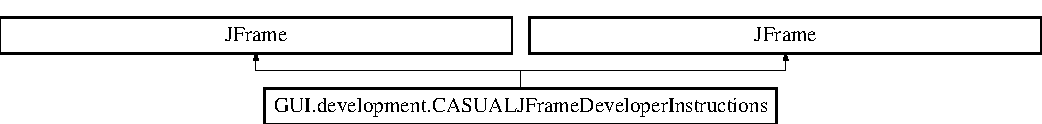
\includegraphics[height=1.671642cm]{classGUI_1_1development_1_1CASUALJFrameDeveloperInstructions}
\end{center}
\end{figure}
\subsection*{Public Member Functions}
\begin{DoxyCompactItemize}
\item 
\hyperlink{classGUI_1_1development_1_1CASUALJFrameDeveloperInstructions_a032e50fd2b2444c584e5dc9dd4ac1495}{C\-A\-S\-U\-A\-L\-J\-Frame\-Developer\-Instructions} ()
\item 
\hyperlink{classGUI_1_1development_1_1CASUALJFrameDeveloperInstructions_a032e50fd2b2444c584e5dc9dd4ac1495}{C\-A\-S\-U\-A\-L\-J\-Frame\-Developer\-Instructions} ()
\end{DoxyCompactItemize}
\subsection*{Static Public Member Functions}
\begin{DoxyCompactItemize}
\item 
static void \hyperlink{classGUI_1_1development_1_1CASUALJFrameDeveloperInstructions_aa7060624c791d6584f86c3319140ba6f}{main} ()
\item 
static void \hyperlink{classGUI_1_1development_1_1CASUALJFrameDeveloperInstructions_aa7060624c791d6584f86c3319140ba6f}{main} ()
\end{DoxyCompactItemize}


\subsection{Detailed Description}
\begin{DoxyAuthor}{Author}
adam 
\end{DoxyAuthor}


\subsection{Constructor \& Destructor Documentation}
\hypertarget{classGUI_1_1development_1_1CASUALJFrameDeveloperInstructions_a032e50fd2b2444c584e5dc9dd4ac1495}{\index{G\-U\-I\-::development\-::\-C\-A\-S\-U\-A\-L\-J\-Frame\-Developer\-Instructions@{G\-U\-I\-::development\-::\-C\-A\-S\-U\-A\-L\-J\-Frame\-Developer\-Instructions}!C\-A\-S\-U\-A\-L\-J\-Frame\-Developer\-Instructions@{C\-A\-S\-U\-A\-L\-J\-Frame\-Developer\-Instructions}}
\index{C\-A\-S\-U\-A\-L\-J\-Frame\-Developer\-Instructions@{C\-A\-S\-U\-A\-L\-J\-Frame\-Developer\-Instructions}!GUI::development::CASUALJFrameDeveloperInstructions@{G\-U\-I\-::development\-::\-C\-A\-S\-U\-A\-L\-J\-Frame\-Developer\-Instructions}}
\subsubsection[{C\-A\-S\-U\-A\-L\-J\-Frame\-Developer\-Instructions}]{\setlength{\rightskip}{0pt plus 5cm}G\-U\-I.\-development.\-C\-A\-S\-U\-A\-L\-J\-Frame\-Developer\-Instructions.\-C\-A\-S\-U\-A\-L\-J\-Frame\-Developer\-Instructions (
\begin{DoxyParamCaption}
{}
\end{DoxyParamCaption}
)}}\label{classGUI_1_1development_1_1CASUALJFrameDeveloperInstructions_a032e50fd2b2444c584e5dc9dd4ac1495}
Creates new form C\-A\-S\-U\-A\-L\-Developer\-Instructions \hypertarget{classGUI_1_1development_1_1CASUALJFrameDeveloperInstructions_a032e50fd2b2444c584e5dc9dd4ac1495}{\index{G\-U\-I\-::development\-::\-C\-A\-S\-U\-A\-L\-J\-Frame\-Developer\-Instructions@{G\-U\-I\-::development\-::\-C\-A\-S\-U\-A\-L\-J\-Frame\-Developer\-Instructions}!C\-A\-S\-U\-A\-L\-J\-Frame\-Developer\-Instructions@{C\-A\-S\-U\-A\-L\-J\-Frame\-Developer\-Instructions}}
\index{C\-A\-S\-U\-A\-L\-J\-Frame\-Developer\-Instructions@{C\-A\-S\-U\-A\-L\-J\-Frame\-Developer\-Instructions}!GUI::development::CASUALJFrameDeveloperInstructions@{G\-U\-I\-::development\-::\-C\-A\-S\-U\-A\-L\-J\-Frame\-Developer\-Instructions}}
\subsubsection[{C\-A\-S\-U\-A\-L\-J\-Frame\-Developer\-Instructions}]{\setlength{\rightskip}{0pt plus 5cm}G\-U\-I.\-development.\-C\-A\-S\-U\-A\-L\-J\-Frame\-Developer\-Instructions.\-C\-A\-S\-U\-A\-L\-J\-Frame\-Developer\-Instructions (
\begin{DoxyParamCaption}
{}
\end{DoxyParamCaption}
)}}\label{classGUI_1_1development_1_1CASUALJFrameDeveloperInstructions_a032e50fd2b2444c584e5dc9dd4ac1495}
Creates new form C\-A\-S\-U\-A\-L\-Developer\-Instructions 

\subsection{Member Function Documentation}
\hypertarget{classGUI_1_1development_1_1CASUALJFrameDeveloperInstructions_aa7060624c791d6584f86c3319140ba6f}{\index{G\-U\-I\-::development\-::\-C\-A\-S\-U\-A\-L\-J\-Frame\-Developer\-Instructions@{G\-U\-I\-::development\-::\-C\-A\-S\-U\-A\-L\-J\-Frame\-Developer\-Instructions}!main@{main}}
\index{main@{main}!GUI::development::CASUALJFrameDeveloperInstructions@{G\-U\-I\-::development\-::\-C\-A\-S\-U\-A\-L\-J\-Frame\-Developer\-Instructions}}
\subsubsection[{main}]{\setlength{\rightskip}{0pt plus 5cm}static void G\-U\-I.\-development.\-C\-A\-S\-U\-A\-L\-J\-Frame\-Developer\-Instructions.\-main (
\begin{DoxyParamCaption}
{}
\end{DoxyParamCaption}
)\hspace{0.3cm}{\ttfamily [static]}}}\label{classGUI_1_1development_1_1CASUALJFrameDeveloperInstructions_aa7060624c791d6584f86c3319140ba6f}
starts the developer instructions frame. \hypertarget{classGUI_1_1development_1_1CASUALJFrameDeveloperInstructions_aa7060624c791d6584f86c3319140ba6f}{\index{G\-U\-I\-::development\-::\-C\-A\-S\-U\-A\-L\-J\-Frame\-Developer\-Instructions@{G\-U\-I\-::development\-::\-C\-A\-S\-U\-A\-L\-J\-Frame\-Developer\-Instructions}!main@{main}}
\index{main@{main}!GUI::development::CASUALJFrameDeveloperInstructions@{G\-U\-I\-::development\-::\-C\-A\-S\-U\-A\-L\-J\-Frame\-Developer\-Instructions}}
\subsubsection[{main}]{\setlength{\rightskip}{0pt plus 5cm}static void G\-U\-I.\-development.\-C\-A\-S\-U\-A\-L\-J\-Frame\-Developer\-Instructions.\-main (
\begin{DoxyParamCaption}
{}
\end{DoxyParamCaption}
)\hspace{0.3cm}{\ttfamily [static]}}}\label{classGUI_1_1development_1_1CASUALJFrameDeveloperInstructions_aa7060624c791d6584f86c3319140ba6f}
starts the developer instructions frame. 

The documentation for this class was generated from the following files\-:\begin{DoxyCompactItemize}
\item 
trunk/\-C\-A\-S\-U\-A\-Lcore/build/classes/\-G\-U\-I/development/C\-A\-S\-U\-A\-L\-J\-Frame\-Developer\-Instructions.\-java\item 
trunk/\-C\-A\-S\-U\-A\-Lcore/src/\-G\-U\-I/development/C\-A\-S\-U\-A\-L\-J\-Frame\-Developer\-Instructions.\-java\end{DoxyCompactItemize}

\hypertarget{classGUI_1_1development_1_1CASUALJFrameLog}{\section{G\-U\-I.\-development.\-C\-A\-S\-U\-A\-L\-J\-Frame\-Log Class Reference}
\label{classGUI_1_1development_1_1CASUALJFrameLog}\index{G\-U\-I.\-development.\-C\-A\-S\-U\-A\-L\-J\-Frame\-Log@{G\-U\-I.\-development.\-C\-A\-S\-U\-A\-L\-J\-Frame\-Log}}
}
Inheritance diagram for G\-U\-I.\-development.\-C\-A\-S\-U\-A\-L\-J\-Frame\-Log\-:\begin{figure}[H]
\begin{center}
\leavevmode
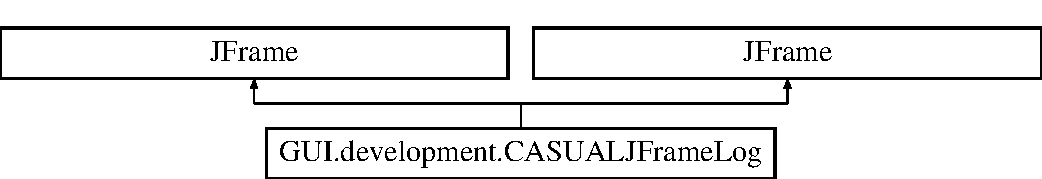
\includegraphics[height=2.000000cm]{classGUI_1_1development_1_1CASUALJFrameLog}
\end{center}
\end{figure}
\subsection*{Public Member Functions}
\begin{DoxyCompactItemize}
\item 
\hyperlink{classGUI_1_1development_1_1CASUALJFrameLog_a9ef7910e9b9d9d8c2b00af212b7e33c0}{C\-A\-S\-U\-A\-L\-J\-Frame\-Log} ()
\item 
\hyperlink{classGUI_1_1development_1_1CASUALJFrameLog_a9ef7910e9b9d9d8c2b00af212b7e33c0}{C\-A\-S\-U\-A\-L\-J\-Frame\-Log} ()
\end{DoxyCompactItemize}
\subsection*{Static Public Member Functions}
\begin{DoxyCompactItemize}
\item 
static void \hyperlink{classGUI_1_1development_1_1CASUALJFrameLog_aad38c589809152549a48f9f65af4f1b6}{main} ()
\item 
static void \hyperlink{classGUI_1_1development_1_1CASUALJFrameLog_aad38c589809152549a48f9f65af4f1b6}{main} ()
\end{DoxyCompactItemize}


\subsection{Detailed Description}
\begin{DoxyAuthor}{Author}
Adam Outler \href{mailto:adamoutler@gmail.com}{\tt adamoutler@gmail.\-com} 
\end{DoxyAuthor}


\subsection{Constructor \& Destructor Documentation}
\hypertarget{classGUI_1_1development_1_1CASUALJFrameLog_a9ef7910e9b9d9d8c2b00af212b7e33c0}{\index{G\-U\-I\-::development\-::\-C\-A\-S\-U\-A\-L\-J\-Frame\-Log@{G\-U\-I\-::development\-::\-C\-A\-S\-U\-A\-L\-J\-Frame\-Log}!C\-A\-S\-U\-A\-L\-J\-Frame\-Log@{C\-A\-S\-U\-A\-L\-J\-Frame\-Log}}
\index{C\-A\-S\-U\-A\-L\-J\-Frame\-Log@{C\-A\-S\-U\-A\-L\-J\-Frame\-Log}!GUI::development::CASUALJFrameLog@{G\-U\-I\-::development\-::\-C\-A\-S\-U\-A\-L\-J\-Frame\-Log}}
\subsubsection[{C\-A\-S\-U\-A\-L\-J\-Frame\-Log}]{\setlength{\rightskip}{0pt plus 5cm}G\-U\-I.\-development.\-C\-A\-S\-U\-A\-L\-J\-Frame\-Log.\-C\-A\-S\-U\-A\-L\-J\-Frame\-Log (
\begin{DoxyParamCaption}
{}
\end{DoxyParamCaption}
)}}\label{classGUI_1_1development_1_1CASUALJFrameLog_a9ef7910e9b9d9d8c2b00af212b7e33c0}
Creates new form C\-A\-S\-U\-A\-L\-Log\-J\-Frame \hypertarget{classGUI_1_1development_1_1CASUALJFrameLog_a9ef7910e9b9d9d8c2b00af212b7e33c0}{\index{G\-U\-I\-::development\-::\-C\-A\-S\-U\-A\-L\-J\-Frame\-Log@{G\-U\-I\-::development\-::\-C\-A\-S\-U\-A\-L\-J\-Frame\-Log}!C\-A\-S\-U\-A\-L\-J\-Frame\-Log@{C\-A\-S\-U\-A\-L\-J\-Frame\-Log}}
\index{C\-A\-S\-U\-A\-L\-J\-Frame\-Log@{C\-A\-S\-U\-A\-L\-J\-Frame\-Log}!GUI::development::CASUALJFrameLog@{G\-U\-I\-::development\-::\-C\-A\-S\-U\-A\-L\-J\-Frame\-Log}}
\subsubsection[{C\-A\-S\-U\-A\-L\-J\-Frame\-Log}]{\setlength{\rightskip}{0pt plus 5cm}G\-U\-I.\-development.\-C\-A\-S\-U\-A\-L\-J\-Frame\-Log.\-C\-A\-S\-U\-A\-L\-J\-Frame\-Log (
\begin{DoxyParamCaption}
{}
\end{DoxyParamCaption}
)}}\label{classGUI_1_1development_1_1CASUALJFrameLog_a9ef7910e9b9d9d8c2b00af212b7e33c0}
Creates new form C\-A\-S\-U\-A\-L\-Log\-J\-Frame 

\subsection{Member Function Documentation}
\hypertarget{classGUI_1_1development_1_1CASUALJFrameLog_aad38c589809152549a48f9f65af4f1b6}{\index{G\-U\-I\-::development\-::\-C\-A\-S\-U\-A\-L\-J\-Frame\-Log@{G\-U\-I\-::development\-::\-C\-A\-S\-U\-A\-L\-J\-Frame\-Log}!main@{main}}
\index{main@{main}!GUI::development::CASUALJFrameLog@{G\-U\-I\-::development\-::\-C\-A\-S\-U\-A\-L\-J\-Frame\-Log}}
\subsubsection[{main}]{\setlength{\rightskip}{0pt plus 5cm}static void G\-U\-I.\-development.\-C\-A\-S\-U\-A\-L\-J\-Frame\-Log.\-main (
\begin{DoxyParamCaption}
{}
\end{DoxyParamCaption}
)\hspace{0.3cm}{\ttfamily [static]}}}\label{classGUI_1_1development_1_1CASUALJFrameLog_aad38c589809152549a48f9f65af4f1b6}
shows the Log j\-Frame \hypertarget{classGUI_1_1development_1_1CASUALJFrameLog_aad38c589809152549a48f9f65af4f1b6}{\index{G\-U\-I\-::development\-::\-C\-A\-S\-U\-A\-L\-J\-Frame\-Log@{G\-U\-I\-::development\-::\-C\-A\-S\-U\-A\-L\-J\-Frame\-Log}!main@{main}}
\index{main@{main}!GUI::development::CASUALJFrameLog@{G\-U\-I\-::development\-::\-C\-A\-S\-U\-A\-L\-J\-Frame\-Log}}
\subsubsection[{main}]{\setlength{\rightskip}{0pt plus 5cm}static void G\-U\-I.\-development.\-C\-A\-S\-U\-A\-L\-J\-Frame\-Log.\-main (
\begin{DoxyParamCaption}
{}
\end{DoxyParamCaption}
)\hspace{0.3cm}{\ttfamily [static]}}}\label{classGUI_1_1development_1_1CASUALJFrameLog_aad38c589809152549a48f9f65af4f1b6}
shows the Log j\-Frame 

The documentation for this class was generated from the following files\-:\begin{DoxyCompactItemize}
\item 
trunk/\-C\-A\-S\-U\-A\-Lcore/build/classes/\-G\-U\-I/development/C\-A\-S\-U\-A\-L\-J\-Frame\-Log.\-java\item 
trunk/\-C\-A\-S\-U\-A\-Lcore/src/\-G\-U\-I/development/C\-A\-S\-U\-A\-L\-J\-Frame\-Log.\-java\end{DoxyCompactItemize}

\hypertarget{classGUI_1_1development_1_1CASUALJFrameMain}{\section{G\-U\-I.\-development.\-C\-A\-S\-U\-A\-L\-J\-Frame\-Main Class Reference}
\label{classGUI_1_1development_1_1CASUALJFrameMain}\index{G\-U\-I.\-development.\-C\-A\-S\-U\-A\-L\-J\-Frame\-Main@{G\-U\-I.\-development.\-C\-A\-S\-U\-A\-L\-J\-Frame\-Main}}
}
Inheritance diagram for G\-U\-I.\-development.\-C\-A\-S\-U\-A\-L\-J\-Frame\-Main\-:\begin{figure}[H]
\begin{center}
\leavevmode
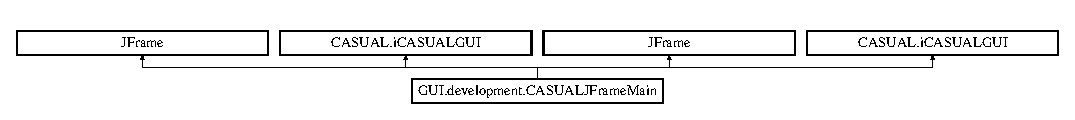
\includegraphics[height=1.166667cm]{classGUI_1_1development_1_1CASUALJFrameMain}
\end{center}
\end{figure}
\subsection*{Public Member Functions}
\begin{DoxyCompactItemize}
\item 
\hyperlink{classGUI_1_1development_1_1CASUALJFrameMain_ac484fbc9062062c993329838cc699127}{C\-A\-S\-U\-A\-L\-J\-Frame\-Main} ()
\item 
void \hyperlink{classGUI_1_1development_1_1CASUALJFrameMain_a019f07e0dcd01688f121d01a6a4f08fb}{Start\-Button\-Action\-Performed} ()
\item 
void \hyperlink{classGUI_1_1development_1_1CASUALJFrameMain_ab5a2bd6f9960330e92ec832a037d8475}{set\-Progress\-Bar} (int value)
\item 
void \hyperlink{classGUI_1_1development_1_1CASUALJFrameMain_aea01e24b1f4fd89b0b362527eb07bc9b}{set\-Progress\-Bar\-Max} (int value)
\item 
String \hyperlink{classGUI_1_1development_1_1CASUALJFrameMain_a65473b796550f93cd0a64fbdc008e321}{combo\-Box\-Get\-Selected\-Item} ()
\item 
void \hyperlink{classGUI_1_1development_1_1CASUALJFrameMain_ad67026cebd68aaa9d5e50a1d772e890b}{combo\-Box\-Script\-Selector\-Add\-New\-Item} (String item)
\item 
void \hyperlink{classGUI_1_1development_1_1CASUALJFrameMain_a6abde49bfe2650f447b5c6abc7d6f077}{set\-Status\-Label\-Icon} (String Icon, String Text)
\item 
void \hyperlink{classGUI_1_1development_1_1CASUALJFrameMain_ad655b0e480491023e7ad25af422c95a9}{set\-Status\-Message\-Label} (String text)
\item 
boolean \hyperlink{classGUI_1_1development_1_1CASUALJFrameMain_af0f386b4ecdf89d6eaa43dc78cd4f6ef}{get\-Control\-Status} ()
\item 
boolean \hyperlink{classGUI_1_1development_1_1CASUALJFrameMain_ae8a8f3e56ff374c6274633ed621dc815}{enable\-Controls} (boolean status)
\item 
void \hyperlink{classGUI_1_1development_1_1CASUALJFrameMain_ab21ac8cd692ec2a63ae0339bb68e374e}{set\-Window\-Banner\-Text} (String text)
\item 
void \hyperlink{classGUI_1_1development_1_1CASUALJFrameMain_a9e5b6e12ea7e3967c9f628788e3bc860}{set\-Start\-Button\-Text} (String text)
\item 
void \hyperlink{classGUI_1_1development_1_1CASUALJFrameMain_a61c6f0a35b429a38f63317e05afaf921}{set\-Window\-Banner\-Image} (Buffered\-Image icon, String text)
\item 
void \hyperlink{classGUI_1_1development_1_1CASUALJFrameMain_ad2838f5ac8ff377c58a8423f3eae1be6}{window\-Cosing} (Window\-Event e)
\item 
void \hyperlink{classGUI_1_1development_1_1CASUALJFrameMain_a5c63c8abc79e383d5ebf1d38c4dfcd13}{set\-Script} (\hyperlink{classCASUAL_1_1caspac_1_1Script}{Script} s)
\item 
void \hyperlink{classGUI_1_1development_1_1CASUALJFrameMain_ae49b006965b1e155a86c6c8c7aec1ecb}{set\-C\-A\-S\-P\-A\-C} (\hyperlink{classCASUAL_1_1caspac_1_1Caspac}{Caspac} caspac)
\item 
void \hyperlink{classGUI_1_1development_1_1CASUALJFrameMain_aa715222603235cd4c0e10ccf8ec35c64}{set\-Information\-Scroll\-Border\-Text} (String title)
\item 
\hypertarget{classGUI_1_1development_1_1CASUALJFrameMain_a96d8372cafb7676437d70cd9e8167f7e}{void {\bfseries set\-Visibile} (boolean v)}\label{classGUI_1_1development_1_1CASUALJFrameMain_a96d8372cafb7676437d70cd9e8167f7e}

\item 
void \hyperlink{classGUI_1_1development_1_1CASUALJFrameMain_aacdbe72ec60c691bc5606c3893a52f7d}{device\-Connected} (String mode)
\item 
void \hyperlink{classGUI_1_1development_1_1CASUALJFrameMain_abd52217ac3134fd45343dd6838601f38}{device\-Disconnected} ()
\item 
void \hyperlink{classGUI_1_1development_1_1CASUALJFrameMain_a0bc8b9c2ca823527932c53d869174e90}{device\-Multiple\-Connected} (int number\-Of\-Devices\-Connected)
\item 
void \hyperlink{classGUI_1_1development_1_1CASUALJFrameMain_a798bd91756d5c27d6f5017a8025b4130}{notification\-Permissions\-Required} ()
\item 
void \hyperlink{classGUI_1_1development_1_1CASUALJFrameMain_a4450abb55d30b94308914af44ef4ee98}{notification\-C\-A\-S\-U\-A\-L\-Sound} ()
\item 
void \hyperlink{classGUI_1_1development_1_1CASUALJFrameMain_a34444561be5204262b95aa6001c4aac1}{notification\-Input\-Requested} ()
\item 
void \hyperlink{classGUI_1_1development_1_1CASUALJFrameMain_a1fe1b03a2ad5aa30c5c8fe208813d4f6}{notification\-General} ()
\item 
void \hyperlink{classGUI_1_1development_1_1CASUALJFrameMain_ad90ba0f96765dfa612ccb92cccecbe98}{notification\-Request\-To\-Continue} ()
\item 
void \hyperlink{classGUI_1_1development_1_1CASUALJFrameMain_a442ecb84833fd7e90fbe97fcb3feb1e7}{notification\-User\-Action\-Is\-Required} ()
\item 
\hyperlink{classGUI_1_1development_1_1CASUALJFrameMain_ac484fbc9062062c993329838cc699127}{C\-A\-S\-U\-A\-L\-J\-Frame\-Main} ()
\item 
void \hyperlink{classGUI_1_1development_1_1CASUALJFrameMain_a019f07e0dcd01688f121d01a6a4f08fb}{Start\-Button\-Action\-Performed} ()
\item 
void \hyperlink{classGUI_1_1development_1_1CASUALJFrameMain_ab5a2bd6f9960330e92ec832a037d8475}{set\-Progress\-Bar} (int value)
\item 
void \hyperlink{classGUI_1_1development_1_1CASUALJFrameMain_aea01e24b1f4fd89b0b362527eb07bc9b}{set\-Progress\-Bar\-Max} (int value)
\item 
String \hyperlink{classGUI_1_1development_1_1CASUALJFrameMain_a65473b796550f93cd0a64fbdc008e321}{combo\-Box\-Get\-Selected\-Item} ()
\item 
void \hyperlink{classGUI_1_1development_1_1CASUALJFrameMain_ad67026cebd68aaa9d5e50a1d772e890b}{combo\-Box\-Script\-Selector\-Add\-New\-Item} (String item)
\item 
void \hyperlink{classGUI_1_1development_1_1CASUALJFrameMain_a6abde49bfe2650f447b5c6abc7d6f077}{set\-Status\-Label\-Icon} (String Icon, String Text)
\item 
void \hyperlink{classGUI_1_1development_1_1CASUALJFrameMain_ad655b0e480491023e7ad25af422c95a9}{set\-Status\-Message\-Label} (String text)
\item 
boolean \hyperlink{classGUI_1_1development_1_1CASUALJFrameMain_af0f386b4ecdf89d6eaa43dc78cd4f6ef}{get\-Control\-Status} ()
\item 
boolean \hyperlink{classGUI_1_1development_1_1CASUALJFrameMain_ae8a8f3e56ff374c6274633ed621dc815}{enable\-Controls} (boolean status)
\item 
void \hyperlink{classGUI_1_1development_1_1CASUALJFrameMain_ab21ac8cd692ec2a63ae0339bb68e374e}{set\-Window\-Banner\-Text} (String text)
\item 
void \hyperlink{classGUI_1_1development_1_1CASUALJFrameMain_a9e5b6e12ea7e3967c9f628788e3bc860}{set\-Start\-Button\-Text} (String text)
\item 
void \hyperlink{classGUI_1_1development_1_1CASUALJFrameMain_a61c6f0a35b429a38f63317e05afaf921}{set\-Window\-Banner\-Image} (Buffered\-Image icon, String text)
\item 
void \hyperlink{classGUI_1_1development_1_1CASUALJFrameMain_ad2838f5ac8ff377c58a8423f3eae1be6}{window\-Cosing} (Window\-Event e)
\item 
void \hyperlink{classGUI_1_1development_1_1CASUALJFrameMain_a5c63c8abc79e383d5ebf1d38c4dfcd13}{set\-Script} (\hyperlink{classCASUAL_1_1caspac_1_1Script}{Script} s)
\item 
void \hyperlink{classGUI_1_1development_1_1CASUALJFrameMain_ae49b006965b1e155a86c6c8c7aec1ecb}{set\-C\-A\-S\-P\-A\-C} (\hyperlink{classCASUAL_1_1caspac_1_1Caspac}{Caspac} caspac)
\item 
void \hyperlink{classGUI_1_1development_1_1CASUALJFrameMain_aa715222603235cd4c0e10ccf8ec35c64}{set\-Information\-Scroll\-Border\-Text} (String title)
\item 
\hypertarget{classGUI_1_1development_1_1CASUALJFrameMain_a96d8372cafb7676437d70cd9e8167f7e}{void {\bfseries set\-Visibile} (boolean v)}\label{classGUI_1_1development_1_1CASUALJFrameMain_a96d8372cafb7676437d70cd9e8167f7e}

\item 
void \hyperlink{classGUI_1_1development_1_1CASUALJFrameMain_aacdbe72ec60c691bc5606c3893a52f7d}{device\-Connected} (String mode)
\item 
void \hyperlink{classGUI_1_1development_1_1CASUALJFrameMain_abd52217ac3134fd45343dd6838601f38}{device\-Disconnected} ()
\item 
void \hyperlink{classGUI_1_1development_1_1CASUALJFrameMain_a0bc8b9c2ca823527932c53d869174e90}{device\-Multiple\-Connected} (int number\-Of\-Devices\-Connected)
\item 
void \hyperlink{classGUI_1_1development_1_1CASUALJFrameMain_a798bd91756d5c27d6f5017a8025b4130}{notification\-Permissions\-Required} ()
\item 
void \hyperlink{classGUI_1_1development_1_1CASUALJFrameMain_a4450abb55d30b94308914af44ef4ee98}{notification\-C\-A\-S\-U\-A\-L\-Sound} ()
\item 
void \hyperlink{classGUI_1_1development_1_1CASUALJFrameMain_a34444561be5204262b95aa6001c4aac1}{notification\-Input\-Requested} ()
\item 
void \hyperlink{classGUI_1_1development_1_1CASUALJFrameMain_a1fe1b03a2ad5aa30c5c8fe208813d4f6}{notification\-General} ()
\item 
void \hyperlink{classGUI_1_1development_1_1CASUALJFrameMain_ad90ba0f96765dfa612ccb92cccecbe98}{notification\-Request\-To\-Continue} ()
\item 
void \hyperlink{classGUI_1_1development_1_1CASUALJFrameMain_a442ecb84833fd7e90fbe97fcb3feb1e7}{notification\-User\-Action\-Is\-Required} ()
\end{DoxyCompactItemize}
\subsection*{Static Public Attributes}
\begin{DoxyCompactItemize}
\item 
\hypertarget{classGUI_1_1development_1_1CASUALJFrameMain_a72d64498ea091c25c674d3d6630875c2}{static javax.\-swing.\-J\-Text\-Pane {\bfseries Progress\-Area}}\label{classGUI_1_1development_1_1CASUALJFrameMain_a72d64498ea091c25c674d3d6630875c2}

\end{DoxyCompactItemize}
\subsection*{Protected Member Functions}
\begin{DoxyCompactItemize}
\item 
Image\-Icon \hyperlink{classGUI_1_1development_1_1CASUALJFrameMain_a77e9e48b60846af1afd1c3ba9867721d}{create\-Image\-Icon} (String path, String description)
\item 
Image\-Icon \hyperlink{classGUI_1_1development_1_1CASUALJFrameMain_a77e9e48b60846af1afd1c3ba9867721d}{create\-Image\-Icon} (String path, String description)
\end{DoxyCompactItemize}


\subsection{Detailed Description}
\begin{DoxyAuthor}{Author}
adam 
\end{DoxyAuthor}


\subsection{Constructor \& Destructor Documentation}
\hypertarget{classGUI_1_1development_1_1CASUALJFrameMain_ac484fbc9062062c993329838cc699127}{\index{G\-U\-I\-::development\-::\-C\-A\-S\-U\-A\-L\-J\-Frame\-Main@{G\-U\-I\-::development\-::\-C\-A\-S\-U\-A\-L\-J\-Frame\-Main}!C\-A\-S\-U\-A\-L\-J\-Frame\-Main@{C\-A\-S\-U\-A\-L\-J\-Frame\-Main}}
\index{C\-A\-S\-U\-A\-L\-J\-Frame\-Main@{C\-A\-S\-U\-A\-L\-J\-Frame\-Main}!GUI::development::CASUALJFrameMain@{G\-U\-I\-::development\-::\-C\-A\-S\-U\-A\-L\-J\-Frame\-Main}}
\subsubsection[{C\-A\-S\-U\-A\-L\-J\-Frame\-Main}]{\setlength{\rightskip}{0pt plus 5cm}G\-U\-I.\-development.\-C\-A\-S\-U\-A\-L\-J\-Frame\-Main.\-C\-A\-S\-U\-A\-L\-J\-Frame\-Main (
\begin{DoxyParamCaption}
{}
\end{DoxyParamCaption}
)}}\label{classGUI_1_1development_1_1CASUALJFrameMain_ac484fbc9062062c993329838cc699127}
Creates new form C\-A\-S\-U\-A\-L\-J\-Frame2 \hypertarget{classGUI_1_1development_1_1CASUALJFrameMain_ac484fbc9062062c993329838cc699127}{\index{G\-U\-I\-::development\-::\-C\-A\-S\-U\-A\-L\-J\-Frame\-Main@{G\-U\-I\-::development\-::\-C\-A\-S\-U\-A\-L\-J\-Frame\-Main}!C\-A\-S\-U\-A\-L\-J\-Frame\-Main@{C\-A\-S\-U\-A\-L\-J\-Frame\-Main}}
\index{C\-A\-S\-U\-A\-L\-J\-Frame\-Main@{C\-A\-S\-U\-A\-L\-J\-Frame\-Main}!GUI::development::CASUALJFrameMain@{G\-U\-I\-::development\-::\-C\-A\-S\-U\-A\-L\-J\-Frame\-Main}}
\subsubsection[{C\-A\-S\-U\-A\-L\-J\-Frame\-Main}]{\setlength{\rightskip}{0pt plus 5cm}G\-U\-I.\-development.\-C\-A\-S\-U\-A\-L\-J\-Frame\-Main.\-C\-A\-S\-U\-A\-L\-J\-Frame\-Main (
\begin{DoxyParamCaption}
{}
\end{DoxyParamCaption}
)}}\label{classGUI_1_1development_1_1CASUALJFrameMain_ac484fbc9062062c993329838cc699127}
Creates new form C\-A\-S\-U\-A\-L\-J\-Frame2 

\subsection{Member Function Documentation}
\hypertarget{classGUI_1_1development_1_1CASUALJFrameMain_a65473b796550f93cd0a64fbdc008e321}{\index{G\-U\-I\-::development\-::\-C\-A\-S\-U\-A\-L\-J\-Frame\-Main@{G\-U\-I\-::development\-::\-C\-A\-S\-U\-A\-L\-J\-Frame\-Main}!combo\-Box\-Get\-Selected\-Item@{combo\-Box\-Get\-Selected\-Item}}
\index{combo\-Box\-Get\-Selected\-Item@{combo\-Box\-Get\-Selected\-Item}!GUI::development::CASUALJFrameMain@{G\-U\-I\-::development\-::\-C\-A\-S\-U\-A\-L\-J\-Frame\-Main}}
\subsubsection[{combo\-Box\-Get\-Selected\-Item}]{\setlength{\rightskip}{0pt plus 5cm}String G\-U\-I.\-development.\-C\-A\-S\-U\-A\-L\-J\-Frame\-Main.\-combo\-Box\-Get\-Selected\-Item (
\begin{DoxyParamCaption}
{}
\end{DoxyParamCaption}
)}}\label{classGUI_1_1development_1_1CASUALJFrameMain_a65473b796550f93cd0a64fbdc008e321}
gets the selected combobox item.

\begin{DoxyReturn}{Returns}
selected item in combobox 
\end{DoxyReturn}


Implements \hyperlink{interfaceCASUAL_1_1iCASUALGUI_a842659e4a515bdb9558082d0f1232f30}{C\-A\-S\-U\-A\-L.\-i\-C\-A\-S\-U\-A\-L\-G\-U\-I}.

\hypertarget{classGUI_1_1development_1_1CASUALJFrameMain_a65473b796550f93cd0a64fbdc008e321}{\index{G\-U\-I\-::development\-::\-C\-A\-S\-U\-A\-L\-J\-Frame\-Main@{G\-U\-I\-::development\-::\-C\-A\-S\-U\-A\-L\-J\-Frame\-Main}!combo\-Box\-Get\-Selected\-Item@{combo\-Box\-Get\-Selected\-Item}}
\index{combo\-Box\-Get\-Selected\-Item@{combo\-Box\-Get\-Selected\-Item}!GUI::development::CASUALJFrameMain@{G\-U\-I\-::development\-::\-C\-A\-S\-U\-A\-L\-J\-Frame\-Main}}
\subsubsection[{combo\-Box\-Get\-Selected\-Item}]{\setlength{\rightskip}{0pt plus 5cm}String G\-U\-I.\-development.\-C\-A\-S\-U\-A\-L\-J\-Frame\-Main.\-combo\-Box\-Get\-Selected\-Item (
\begin{DoxyParamCaption}
{}
\end{DoxyParamCaption}
)}}\label{classGUI_1_1development_1_1CASUALJFrameMain_a65473b796550f93cd0a64fbdc008e321}
gets the selected combobox item.

\begin{DoxyReturn}{Returns}
selected item in combobox 
\end{DoxyReturn}


Implements \hyperlink{interfaceCASUAL_1_1iCASUALGUI_a842659e4a515bdb9558082d0f1232f30}{C\-A\-S\-U\-A\-L.\-i\-C\-A\-S\-U\-A\-L\-G\-U\-I}.

\hypertarget{classGUI_1_1development_1_1CASUALJFrameMain_ad67026cebd68aaa9d5e50a1d772e890b}{\index{G\-U\-I\-::development\-::\-C\-A\-S\-U\-A\-L\-J\-Frame\-Main@{G\-U\-I\-::development\-::\-C\-A\-S\-U\-A\-L\-J\-Frame\-Main}!combo\-Box\-Script\-Selector\-Add\-New\-Item@{combo\-Box\-Script\-Selector\-Add\-New\-Item}}
\index{combo\-Box\-Script\-Selector\-Add\-New\-Item@{combo\-Box\-Script\-Selector\-Add\-New\-Item}!GUI::development::CASUALJFrameMain@{G\-U\-I\-::development\-::\-C\-A\-S\-U\-A\-L\-J\-Frame\-Main}}
\subsubsection[{combo\-Box\-Script\-Selector\-Add\-New\-Item}]{\setlength{\rightskip}{0pt plus 5cm}void G\-U\-I.\-development.\-C\-A\-S\-U\-A\-L\-J\-Frame\-Main.\-combo\-Box\-Script\-Selector\-Add\-New\-Item (
\begin{DoxyParamCaption}
\item[{String}]{item}
\end{DoxyParamCaption}
)}}\label{classGUI_1_1development_1_1CASUALJFrameMain_ad67026cebd68aaa9d5e50a1d772e890b}
adds an item to the combo box


\begin{DoxyParams}{Parameters}
{\em item} & item to add \\
\hline
\end{DoxyParams}


Implements \hyperlink{interfaceCASUAL_1_1iCASUALGUI_a27a26714a3f630a69be0138fa8393979}{C\-A\-S\-U\-A\-L.\-i\-C\-A\-S\-U\-A\-L\-G\-U\-I}.

\hypertarget{classGUI_1_1development_1_1CASUALJFrameMain_ad67026cebd68aaa9d5e50a1d772e890b}{\index{G\-U\-I\-::development\-::\-C\-A\-S\-U\-A\-L\-J\-Frame\-Main@{G\-U\-I\-::development\-::\-C\-A\-S\-U\-A\-L\-J\-Frame\-Main}!combo\-Box\-Script\-Selector\-Add\-New\-Item@{combo\-Box\-Script\-Selector\-Add\-New\-Item}}
\index{combo\-Box\-Script\-Selector\-Add\-New\-Item@{combo\-Box\-Script\-Selector\-Add\-New\-Item}!GUI::development::CASUALJFrameMain@{G\-U\-I\-::development\-::\-C\-A\-S\-U\-A\-L\-J\-Frame\-Main}}
\subsubsection[{combo\-Box\-Script\-Selector\-Add\-New\-Item}]{\setlength{\rightskip}{0pt plus 5cm}void G\-U\-I.\-development.\-C\-A\-S\-U\-A\-L\-J\-Frame\-Main.\-combo\-Box\-Script\-Selector\-Add\-New\-Item (
\begin{DoxyParamCaption}
\item[{String}]{item}
\end{DoxyParamCaption}
)}}\label{classGUI_1_1development_1_1CASUALJFrameMain_ad67026cebd68aaa9d5e50a1d772e890b}
adds an item to the combo box


\begin{DoxyParams}{Parameters}
{\em item} & item to add \\
\hline
\end{DoxyParams}


Implements \hyperlink{interfaceCASUAL_1_1iCASUALGUI_a27a26714a3f630a69be0138fa8393979}{C\-A\-S\-U\-A\-L.\-i\-C\-A\-S\-U\-A\-L\-G\-U\-I}.

\hypertarget{classGUI_1_1development_1_1CASUALJFrameMain_a77e9e48b60846af1afd1c3ba9867721d}{\index{G\-U\-I\-::development\-::\-C\-A\-S\-U\-A\-L\-J\-Frame\-Main@{G\-U\-I\-::development\-::\-C\-A\-S\-U\-A\-L\-J\-Frame\-Main}!create\-Image\-Icon@{create\-Image\-Icon}}
\index{create\-Image\-Icon@{create\-Image\-Icon}!GUI::development::CASUALJFrameMain@{G\-U\-I\-::development\-::\-C\-A\-S\-U\-A\-L\-J\-Frame\-Main}}
\subsubsection[{create\-Image\-Icon}]{\setlength{\rightskip}{0pt plus 5cm}Image\-Icon G\-U\-I.\-development.\-C\-A\-S\-U\-A\-L\-J\-Frame\-Main.\-create\-Image\-Icon (
\begin{DoxyParamCaption}
\item[{String}]{path, }
\item[{String}]{description}
\end{DoxyParamCaption}
)\hspace{0.3cm}{\ttfamily [protected]}}}\label{classGUI_1_1development_1_1CASUALJFrameMain_a77e9e48b60846af1afd1c3ba9867721d}
takes a resource and turns it into an Image\-Icon


\begin{DoxyParams}{Parameters}
{\em path} & pat to resource \\
\hline
{\em description} & icon description \\
\hline
\end{DoxyParams}
\begin{DoxyReturn}{Returns}
an icon 
\end{DoxyReturn}
\hypertarget{classGUI_1_1development_1_1CASUALJFrameMain_a77e9e48b60846af1afd1c3ba9867721d}{\index{G\-U\-I\-::development\-::\-C\-A\-S\-U\-A\-L\-J\-Frame\-Main@{G\-U\-I\-::development\-::\-C\-A\-S\-U\-A\-L\-J\-Frame\-Main}!create\-Image\-Icon@{create\-Image\-Icon}}
\index{create\-Image\-Icon@{create\-Image\-Icon}!GUI::development::CASUALJFrameMain@{G\-U\-I\-::development\-::\-C\-A\-S\-U\-A\-L\-J\-Frame\-Main}}
\subsubsection[{create\-Image\-Icon}]{\setlength{\rightskip}{0pt plus 5cm}Image\-Icon G\-U\-I.\-development.\-C\-A\-S\-U\-A\-L\-J\-Frame\-Main.\-create\-Image\-Icon (
\begin{DoxyParamCaption}
\item[{String}]{path, }
\item[{String}]{description}
\end{DoxyParamCaption}
)\hspace{0.3cm}{\ttfamily [protected]}}}\label{classGUI_1_1development_1_1CASUALJFrameMain_a77e9e48b60846af1afd1c3ba9867721d}
takes a resource and turns it into an Image\-Icon


\begin{DoxyParams}{Parameters}
{\em path} & pat to resource \\
\hline
{\em description} & icon description \\
\hline
\end{DoxyParams}
\begin{DoxyReturn}{Returns}
an icon 
\end{DoxyReturn}
\hypertarget{classGUI_1_1development_1_1CASUALJFrameMain_aacdbe72ec60c691bc5606c3893a52f7d}{\index{G\-U\-I\-::development\-::\-C\-A\-S\-U\-A\-L\-J\-Frame\-Main@{G\-U\-I\-::development\-::\-C\-A\-S\-U\-A\-L\-J\-Frame\-Main}!device\-Connected@{device\-Connected}}
\index{device\-Connected@{device\-Connected}!GUI::development::CASUALJFrameMain@{G\-U\-I\-::development\-::\-C\-A\-S\-U\-A\-L\-J\-Frame\-Main}}
\subsubsection[{device\-Connected}]{\setlength{\rightskip}{0pt plus 5cm}void G\-U\-I.\-development.\-C\-A\-S\-U\-A\-L\-J\-Frame\-Main.\-device\-Connected (
\begin{DoxyParamCaption}
\item[{String}]{mode}
\end{DoxyParamCaption}
)}}\label{classGUI_1_1development_1_1CASUALJFrameMain_aacdbe72ec60c691bc5606c3893a52f7d}
called when device is connected 
\begin{DoxyParams}{Parameters}
{\em mode} & adb/fastboot/heimdall/flashtool \\
\hline
\end{DoxyParams}


Implements \hyperlink{interfaceCASUAL_1_1iCASUALGUI_a1d118a6e2fa316d2a1e90256a0572795}{C\-A\-S\-U\-A\-L.\-i\-C\-A\-S\-U\-A\-L\-G\-U\-I}.

\hypertarget{classGUI_1_1development_1_1CASUALJFrameMain_aacdbe72ec60c691bc5606c3893a52f7d}{\index{G\-U\-I\-::development\-::\-C\-A\-S\-U\-A\-L\-J\-Frame\-Main@{G\-U\-I\-::development\-::\-C\-A\-S\-U\-A\-L\-J\-Frame\-Main}!device\-Connected@{device\-Connected}}
\index{device\-Connected@{device\-Connected}!GUI::development::CASUALJFrameMain@{G\-U\-I\-::development\-::\-C\-A\-S\-U\-A\-L\-J\-Frame\-Main}}
\subsubsection[{device\-Connected}]{\setlength{\rightskip}{0pt plus 5cm}void G\-U\-I.\-development.\-C\-A\-S\-U\-A\-L\-J\-Frame\-Main.\-device\-Connected (
\begin{DoxyParamCaption}
\item[{String}]{mode}
\end{DoxyParamCaption}
)}}\label{classGUI_1_1development_1_1CASUALJFrameMain_aacdbe72ec60c691bc5606c3893a52f7d}
called when device is connected 
\begin{DoxyParams}{Parameters}
{\em mode} & adb/fastboot/heimdall/flashtool \\
\hline
\end{DoxyParams}


Implements \hyperlink{interfaceCASUAL_1_1iCASUALGUI_a1d118a6e2fa316d2a1e90256a0572795}{C\-A\-S\-U\-A\-L.\-i\-C\-A\-S\-U\-A\-L\-G\-U\-I}.

\hypertarget{classGUI_1_1development_1_1CASUALJFrameMain_abd52217ac3134fd45343dd6838601f38}{\index{G\-U\-I\-::development\-::\-C\-A\-S\-U\-A\-L\-J\-Frame\-Main@{G\-U\-I\-::development\-::\-C\-A\-S\-U\-A\-L\-J\-Frame\-Main}!device\-Disconnected@{device\-Disconnected}}
\index{device\-Disconnected@{device\-Disconnected}!GUI::development::CASUALJFrameMain@{G\-U\-I\-::development\-::\-C\-A\-S\-U\-A\-L\-J\-Frame\-Main}}
\subsubsection[{device\-Disconnected}]{\setlength{\rightskip}{0pt plus 5cm}void G\-U\-I.\-development.\-C\-A\-S\-U\-A\-L\-J\-Frame\-Main.\-device\-Disconnected (
\begin{DoxyParamCaption}
{}
\end{DoxyParamCaption}
)}}\label{classGUI_1_1development_1_1CASUALJFrameMain_abd52217ac3134fd45343dd6838601f38}
Device has disconnected, alert the user 

Implements \hyperlink{interfaceCASUAL_1_1iCASUALGUI_a360c068814d6714ff427d2bced13c6d2}{C\-A\-S\-U\-A\-L.\-i\-C\-A\-S\-U\-A\-L\-G\-U\-I}.

\hypertarget{classGUI_1_1development_1_1CASUALJFrameMain_abd52217ac3134fd45343dd6838601f38}{\index{G\-U\-I\-::development\-::\-C\-A\-S\-U\-A\-L\-J\-Frame\-Main@{G\-U\-I\-::development\-::\-C\-A\-S\-U\-A\-L\-J\-Frame\-Main}!device\-Disconnected@{device\-Disconnected}}
\index{device\-Disconnected@{device\-Disconnected}!GUI::development::CASUALJFrameMain@{G\-U\-I\-::development\-::\-C\-A\-S\-U\-A\-L\-J\-Frame\-Main}}
\subsubsection[{device\-Disconnected}]{\setlength{\rightskip}{0pt plus 5cm}void G\-U\-I.\-development.\-C\-A\-S\-U\-A\-L\-J\-Frame\-Main.\-device\-Disconnected (
\begin{DoxyParamCaption}
{}
\end{DoxyParamCaption}
)}}\label{classGUI_1_1development_1_1CASUALJFrameMain_abd52217ac3134fd45343dd6838601f38}
Device has disconnected, alert the user 

Implements \hyperlink{interfaceCASUAL_1_1iCASUALGUI_a360c068814d6714ff427d2bced13c6d2}{C\-A\-S\-U\-A\-L.\-i\-C\-A\-S\-U\-A\-L\-G\-U\-I}.

\hypertarget{classGUI_1_1development_1_1CASUALJFrameMain_a0bc8b9c2ca823527932c53d869174e90}{\index{G\-U\-I\-::development\-::\-C\-A\-S\-U\-A\-L\-J\-Frame\-Main@{G\-U\-I\-::development\-::\-C\-A\-S\-U\-A\-L\-J\-Frame\-Main}!device\-Multiple\-Connected@{device\-Multiple\-Connected}}
\index{device\-Multiple\-Connected@{device\-Multiple\-Connected}!GUI::development::CASUALJFrameMain@{G\-U\-I\-::development\-::\-C\-A\-S\-U\-A\-L\-J\-Frame\-Main}}
\subsubsection[{device\-Multiple\-Connected}]{\setlength{\rightskip}{0pt plus 5cm}void G\-U\-I.\-development.\-C\-A\-S\-U\-A\-L\-J\-Frame\-Main.\-device\-Multiple\-Connected (
\begin{DoxyParamCaption}
\item[{int}]{number\-Of\-Devices\-Connected}
\end{DoxyParamCaption}
)}}\label{classGUI_1_1development_1_1CASUALJFrameMain_a0bc8b9c2ca823527932c53d869174e90}
multiple devices are detected. only one is allowed 
\begin{DoxyParams}{Parameters}
{\em number\-Of\-Devices\-Connected} & number of devices \\
\hline
\end{DoxyParams}


Implements \hyperlink{interfaceCASUAL_1_1iCASUALGUI_a14f848e7113fb3488549d5c00bd9e751}{C\-A\-S\-U\-A\-L.\-i\-C\-A\-S\-U\-A\-L\-G\-U\-I}.

\hypertarget{classGUI_1_1development_1_1CASUALJFrameMain_a0bc8b9c2ca823527932c53d869174e90}{\index{G\-U\-I\-::development\-::\-C\-A\-S\-U\-A\-L\-J\-Frame\-Main@{G\-U\-I\-::development\-::\-C\-A\-S\-U\-A\-L\-J\-Frame\-Main}!device\-Multiple\-Connected@{device\-Multiple\-Connected}}
\index{device\-Multiple\-Connected@{device\-Multiple\-Connected}!GUI::development::CASUALJFrameMain@{G\-U\-I\-::development\-::\-C\-A\-S\-U\-A\-L\-J\-Frame\-Main}}
\subsubsection[{device\-Multiple\-Connected}]{\setlength{\rightskip}{0pt plus 5cm}void G\-U\-I.\-development.\-C\-A\-S\-U\-A\-L\-J\-Frame\-Main.\-device\-Multiple\-Connected (
\begin{DoxyParamCaption}
\item[{int}]{number\-Of\-Devices\-Connected}
\end{DoxyParamCaption}
)}}\label{classGUI_1_1development_1_1CASUALJFrameMain_a0bc8b9c2ca823527932c53d869174e90}
multiple devices are detected. only one is allowed 
\begin{DoxyParams}{Parameters}
{\em number\-Of\-Devices\-Connected} & number of devices \\
\hline
\end{DoxyParams}


Implements \hyperlink{interfaceCASUAL_1_1iCASUALGUI_a14f848e7113fb3488549d5c00bd9e751}{C\-A\-S\-U\-A\-L.\-i\-C\-A\-S\-U\-A\-L\-G\-U\-I}.

\hypertarget{classGUI_1_1development_1_1CASUALJFrameMain_ae8a8f3e56ff374c6274633ed621dc815}{\index{G\-U\-I\-::development\-::\-C\-A\-S\-U\-A\-L\-J\-Frame\-Main@{G\-U\-I\-::development\-::\-C\-A\-S\-U\-A\-L\-J\-Frame\-Main}!enable\-Controls@{enable\-Controls}}
\index{enable\-Controls@{enable\-Controls}!GUI::development::CASUALJFrameMain@{G\-U\-I\-::development\-::\-C\-A\-S\-U\-A\-L\-J\-Frame\-Main}}
\subsubsection[{enable\-Controls}]{\setlength{\rightskip}{0pt plus 5cm}boolean G\-U\-I.\-development.\-C\-A\-S\-U\-A\-L\-J\-Frame\-Main.\-enable\-Controls (
\begin{DoxyParamCaption}
\item[{boolean}]{status}
\end{DoxyParamCaption}
)}}\label{classGUI_1_1development_1_1CASUALJFrameMain_ae8a8f3e56ff374c6274633ed621dc815}
sets controls status


\begin{DoxyParams}{Parameters}
{\em status} & commanded value \\
\hline
\end{DoxyParams}
\begin{DoxyReturn}{Returns}
true if enabled false if not 
\end{DoxyReturn}


Implements \hyperlink{interfaceCASUAL_1_1iCASUALGUI_a13e5b49519aeda6e1df10ae7680cded9}{C\-A\-S\-U\-A\-L.\-i\-C\-A\-S\-U\-A\-L\-G\-U\-I}.

\hypertarget{classGUI_1_1development_1_1CASUALJFrameMain_ae8a8f3e56ff374c6274633ed621dc815}{\index{G\-U\-I\-::development\-::\-C\-A\-S\-U\-A\-L\-J\-Frame\-Main@{G\-U\-I\-::development\-::\-C\-A\-S\-U\-A\-L\-J\-Frame\-Main}!enable\-Controls@{enable\-Controls}}
\index{enable\-Controls@{enable\-Controls}!GUI::development::CASUALJFrameMain@{G\-U\-I\-::development\-::\-C\-A\-S\-U\-A\-L\-J\-Frame\-Main}}
\subsubsection[{enable\-Controls}]{\setlength{\rightskip}{0pt plus 5cm}boolean G\-U\-I.\-development.\-C\-A\-S\-U\-A\-L\-J\-Frame\-Main.\-enable\-Controls (
\begin{DoxyParamCaption}
\item[{boolean}]{status}
\end{DoxyParamCaption}
)}}\label{classGUI_1_1development_1_1CASUALJFrameMain_ae8a8f3e56ff374c6274633ed621dc815}
sets controls status


\begin{DoxyParams}{Parameters}
{\em status} & commanded value \\
\hline
\end{DoxyParams}
\begin{DoxyReturn}{Returns}
true if enabled false if not 
\end{DoxyReturn}


Implements \hyperlink{interfaceCASUAL_1_1iCASUALGUI_a13e5b49519aeda6e1df10ae7680cded9}{C\-A\-S\-U\-A\-L.\-i\-C\-A\-S\-U\-A\-L\-G\-U\-I}.

\hypertarget{classGUI_1_1development_1_1CASUALJFrameMain_af0f386b4ecdf89d6eaa43dc78cd4f6ef}{\index{G\-U\-I\-::development\-::\-C\-A\-S\-U\-A\-L\-J\-Frame\-Main@{G\-U\-I\-::development\-::\-C\-A\-S\-U\-A\-L\-J\-Frame\-Main}!get\-Control\-Status@{get\-Control\-Status}}
\index{get\-Control\-Status@{get\-Control\-Status}!GUI::development::CASUALJFrameMain@{G\-U\-I\-::development\-::\-C\-A\-S\-U\-A\-L\-J\-Frame\-Main}}
\subsubsection[{get\-Control\-Status}]{\setlength{\rightskip}{0pt plus 5cm}boolean G\-U\-I.\-development.\-C\-A\-S\-U\-A\-L\-J\-Frame\-Main.\-get\-Control\-Status (
\begin{DoxyParamCaption}
{}
\end{DoxyParamCaption}
)}}\label{classGUI_1_1development_1_1CASUALJFrameMain_af0f386b4ecdf89d6eaa43dc78cd4f6ef}
gets the control status

\begin{DoxyReturn}{Returns}
true if enabled 
\end{DoxyReturn}


Implements \hyperlink{interfaceCASUAL_1_1iCASUALGUI_a0da22163bda8a58af87b464429dc3386}{C\-A\-S\-U\-A\-L.\-i\-C\-A\-S\-U\-A\-L\-G\-U\-I}.

\hypertarget{classGUI_1_1development_1_1CASUALJFrameMain_af0f386b4ecdf89d6eaa43dc78cd4f6ef}{\index{G\-U\-I\-::development\-::\-C\-A\-S\-U\-A\-L\-J\-Frame\-Main@{G\-U\-I\-::development\-::\-C\-A\-S\-U\-A\-L\-J\-Frame\-Main}!get\-Control\-Status@{get\-Control\-Status}}
\index{get\-Control\-Status@{get\-Control\-Status}!GUI::development::CASUALJFrameMain@{G\-U\-I\-::development\-::\-C\-A\-S\-U\-A\-L\-J\-Frame\-Main}}
\subsubsection[{get\-Control\-Status}]{\setlength{\rightskip}{0pt plus 5cm}boolean G\-U\-I.\-development.\-C\-A\-S\-U\-A\-L\-J\-Frame\-Main.\-get\-Control\-Status (
\begin{DoxyParamCaption}
{}
\end{DoxyParamCaption}
)}}\label{classGUI_1_1development_1_1CASUALJFrameMain_af0f386b4ecdf89d6eaa43dc78cd4f6ef}
gets the control status

\begin{DoxyReturn}{Returns}
true if enabled 
\end{DoxyReturn}


Implements \hyperlink{interfaceCASUAL_1_1iCASUALGUI_a0da22163bda8a58af87b464429dc3386}{C\-A\-S\-U\-A\-L.\-i\-C\-A\-S\-U\-A\-L\-G\-U\-I}.

\hypertarget{classGUI_1_1development_1_1CASUALJFrameMain_a4450abb55d30b94308914af44ef4ee98}{\index{G\-U\-I\-::development\-::\-C\-A\-S\-U\-A\-L\-J\-Frame\-Main@{G\-U\-I\-::development\-::\-C\-A\-S\-U\-A\-L\-J\-Frame\-Main}!notification\-C\-A\-S\-U\-A\-L\-Sound@{notification\-C\-A\-S\-U\-A\-L\-Sound}}
\index{notification\-C\-A\-S\-U\-A\-L\-Sound@{notification\-C\-A\-S\-U\-A\-L\-Sound}!GUI::development::CASUALJFrameMain@{G\-U\-I\-::development\-::\-C\-A\-S\-U\-A\-L\-J\-Frame\-Main}}
\subsubsection[{notification\-C\-A\-S\-U\-A\-L\-Sound}]{\setlength{\rightskip}{0pt plus 5cm}void G\-U\-I.\-development.\-C\-A\-S\-U\-A\-L\-J\-Frame\-Main.\-notification\-C\-A\-S\-U\-A\-L\-Sound (
\begin{DoxyParamCaption}
{}
\end{DoxyParamCaption}
)}}\label{classGUI_1_1development_1_1CASUALJFrameMain_a4450abb55d30b94308914af44ef4ee98}
Startup event 

Implements \hyperlink{interfaceCASUAL_1_1iCASUALGUI_a8ed1e2eeb8018c79935326542fbe66e7}{C\-A\-S\-U\-A\-L.\-i\-C\-A\-S\-U\-A\-L\-G\-U\-I}.

\hypertarget{classGUI_1_1development_1_1CASUALJFrameMain_a4450abb55d30b94308914af44ef4ee98}{\index{G\-U\-I\-::development\-::\-C\-A\-S\-U\-A\-L\-J\-Frame\-Main@{G\-U\-I\-::development\-::\-C\-A\-S\-U\-A\-L\-J\-Frame\-Main}!notification\-C\-A\-S\-U\-A\-L\-Sound@{notification\-C\-A\-S\-U\-A\-L\-Sound}}
\index{notification\-C\-A\-S\-U\-A\-L\-Sound@{notification\-C\-A\-S\-U\-A\-L\-Sound}!GUI::development::CASUALJFrameMain@{G\-U\-I\-::development\-::\-C\-A\-S\-U\-A\-L\-J\-Frame\-Main}}
\subsubsection[{notification\-C\-A\-S\-U\-A\-L\-Sound}]{\setlength{\rightskip}{0pt plus 5cm}void G\-U\-I.\-development.\-C\-A\-S\-U\-A\-L\-J\-Frame\-Main.\-notification\-C\-A\-S\-U\-A\-L\-Sound (
\begin{DoxyParamCaption}
{}
\end{DoxyParamCaption}
)}}\label{classGUI_1_1development_1_1CASUALJFrameMain_a4450abb55d30b94308914af44ef4ee98}
Startup event 

Implements \hyperlink{interfaceCASUAL_1_1iCASUALGUI_a8ed1e2eeb8018c79935326542fbe66e7}{C\-A\-S\-U\-A\-L.\-i\-C\-A\-S\-U\-A\-L\-G\-U\-I}.

\hypertarget{classGUI_1_1development_1_1CASUALJFrameMain_a1fe1b03a2ad5aa30c5c8fe208813d4f6}{\index{G\-U\-I\-::development\-::\-C\-A\-S\-U\-A\-L\-J\-Frame\-Main@{G\-U\-I\-::development\-::\-C\-A\-S\-U\-A\-L\-J\-Frame\-Main}!notification\-General@{notification\-General}}
\index{notification\-General@{notification\-General}!GUI::development::CASUALJFrameMain@{G\-U\-I\-::development\-::\-C\-A\-S\-U\-A\-L\-J\-Frame\-Main}}
\subsubsection[{notification\-General}]{\setlength{\rightskip}{0pt plus 5cm}void G\-U\-I.\-development.\-C\-A\-S\-U\-A\-L\-J\-Frame\-Main.\-notification\-General (
\begin{DoxyParamCaption}
{}
\end{DoxyParamCaption}
)}}\label{classGUI_1_1development_1_1CASUALJFrameMain_a1fe1b03a2ad5aa30c5c8fe208813d4f6}
A notification has been issued to the user 

Implements \hyperlink{interfaceCASUAL_1_1iCASUALGUI_afb18773fbee213dccef143061f8d8b32}{C\-A\-S\-U\-A\-L.\-i\-C\-A\-S\-U\-A\-L\-G\-U\-I}.

\hypertarget{classGUI_1_1development_1_1CASUALJFrameMain_a1fe1b03a2ad5aa30c5c8fe208813d4f6}{\index{G\-U\-I\-::development\-::\-C\-A\-S\-U\-A\-L\-J\-Frame\-Main@{G\-U\-I\-::development\-::\-C\-A\-S\-U\-A\-L\-J\-Frame\-Main}!notification\-General@{notification\-General}}
\index{notification\-General@{notification\-General}!GUI::development::CASUALJFrameMain@{G\-U\-I\-::development\-::\-C\-A\-S\-U\-A\-L\-J\-Frame\-Main}}
\subsubsection[{notification\-General}]{\setlength{\rightskip}{0pt plus 5cm}void G\-U\-I.\-development.\-C\-A\-S\-U\-A\-L\-J\-Frame\-Main.\-notification\-General (
\begin{DoxyParamCaption}
{}
\end{DoxyParamCaption}
)}}\label{classGUI_1_1development_1_1CASUALJFrameMain_a1fe1b03a2ad5aa30c5c8fe208813d4f6}
A notification has been issued to the user 

Implements \hyperlink{interfaceCASUAL_1_1iCASUALGUI_afb18773fbee213dccef143061f8d8b32}{C\-A\-S\-U\-A\-L.\-i\-C\-A\-S\-U\-A\-L\-G\-U\-I}.

\hypertarget{classGUI_1_1development_1_1CASUALJFrameMain_a34444561be5204262b95aa6001c4aac1}{\index{G\-U\-I\-::development\-::\-C\-A\-S\-U\-A\-L\-J\-Frame\-Main@{G\-U\-I\-::development\-::\-C\-A\-S\-U\-A\-L\-J\-Frame\-Main}!notification\-Input\-Requested@{notification\-Input\-Requested}}
\index{notification\-Input\-Requested@{notification\-Input\-Requested}!GUI::development::CASUALJFrameMain@{G\-U\-I\-::development\-::\-C\-A\-S\-U\-A\-L\-J\-Frame\-Main}}
\subsubsection[{notification\-Input\-Requested}]{\setlength{\rightskip}{0pt plus 5cm}void G\-U\-I.\-development.\-C\-A\-S\-U\-A\-L\-J\-Frame\-Main.\-notification\-Input\-Requested (
\begin{DoxyParamCaption}
{}
\end{DoxyParamCaption}
)}}\label{classGUI_1_1development_1_1CASUALJFrameMain_a34444561be5204262b95aa6001c4aac1}
Input is requested from the user 

Implements \hyperlink{interfaceCASUAL_1_1iCASUALGUI_aadb0d6eaf13ea440f2fde52635686aba}{C\-A\-S\-U\-A\-L.\-i\-C\-A\-S\-U\-A\-L\-G\-U\-I}.

\hypertarget{classGUI_1_1development_1_1CASUALJFrameMain_a34444561be5204262b95aa6001c4aac1}{\index{G\-U\-I\-::development\-::\-C\-A\-S\-U\-A\-L\-J\-Frame\-Main@{G\-U\-I\-::development\-::\-C\-A\-S\-U\-A\-L\-J\-Frame\-Main}!notification\-Input\-Requested@{notification\-Input\-Requested}}
\index{notification\-Input\-Requested@{notification\-Input\-Requested}!GUI::development::CASUALJFrameMain@{G\-U\-I\-::development\-::\-C\-A\-S\-U\-A\-L\-J\-Frame\-Main}}
\subsubsection[{notification\-Input\-Requested}]{\setlength{\rightskip}{0pt plus 5cm}void G\-U\-I.\-development.\-C\-A\-S\-U\-A\-L\-J\-Frame\-Main.\-notification\-Input\-Requested (
\begin{DoxyParamCaption}
{}
\end{DoxyParamCaption}
)}}\label{classGUI_1_1development_1_1CASUALJFrameMain_a34444561be5204262b95aa6001c4aac1}
Input is requested from the user 

Implements \hyperlink{interfaceCASUAL_1_1iCASUALGUI_aadb0d6eaf13ea440f2fde52635686aba}{C\-A\-S\-U\-A\-L.\-i\-C\-A\-S\-U\-A\-L\-G\-U\-I}.

\hypertarget{classGUI_1_1development_1_1CASUALJFrameMain_a798bd91756d5c27d6f5017a8025b4130}{\index{G\-U\-I\-::development\-::\-C\-A\-S\-U\-A\-L\-J\-Frame\-Main@{G\-U\-I\-::development\-::\-C\-A\-S\-U\-A\-L\-J\-Frame\-Main}!notification\-Permissions\-Required@{notification\-Permissions\-Required}}
\index{notification\-Permissions\-Required@{notification\-Permissions\-Required}!GUI::development::CASUALJFrameMain@{G\-U\-I\-::development\-::\-C\-A\-S\-U\-A\-L\-J\-Frame\-Main}}
\subsubsection[{notification\-Permissions\-Required}]{\setlength{\rightskip}{0pt plus 5cm}void G\-U\-I.\-development.\-C\-A\-S\-U\-A\-L\-J\-Frame\-Main.\-notification\-Permissions\-Required (
\begin{DoxyParamCaption}
{}
\end{DoxyParamCaption}
)}}\label{classGUI_1_1development_1_1CASUALJFrameMain_a798bd91756d5c27d6f5017a8025b4130}
permissions escillation is required 

Implements \hyperlink{interfaceCASUAL_1_1iCASUALGUI_a601a31c3779aaf519ce85b77cc2ca753}{C\-A\-S\-U\-A\-L.\-i\-C\-A\-S\-U\-A\-L\-G\-U\-I}.

\hypertarget{classGUI_1_1development_1_1CASUALJFrameMain_a798bd91756d5c27d6f5017a8025b4130}{\index{G\-U\-I\-::development\-::\-C\-A\-S\-U\-A\-L\-J\-Frame\-Main@{G\-U\-I\-::development\-::\-C\-A\-S\-U\-A\-L\-J\-Frame\-Main}!notification\-Permissions\-Required@{notification\-Permissions\-Required}}
\index{notification\-Permissions\-Required@{notification\-Permissions\-Required}!GUI::development::CASUALJFrameMain@{G\-U\-I\-::development\-::\-C\-A\-S\-U\-A\-L\-J\-Frame\-Main}}
\subsubsection[{notification\-Permissions\-Required}]{\setlength{\rightskip}{0pt plus 5cm}void G\-U\-I.\-development.\-C\-A\-S\-U\-A\-L\-J\-Frame\-Main.\-notification\-Permissions\-Required (
\begin{DoxyParamCaption}
{}
\end{DoxyParamCaption}
)}}\label{classGUI_1_1development_1_1CASUALJFrameMain_a798bd91756d5c27d6f5017a8025b4130}
permissions escillation is required 

Implements \hyperlink{interfaceCASUAL_1_1iCASUALGUI_a601a31c3779aaf519ce85b77cc2ca753}{C\-A\-S\-U\-A\-L.\-i\-C\-A\-S\-U\-A\-L\-G\-U\-I}.

\hypertarget{classGUI_1_1development_1_1CASUALJFrameMain_ad90ba0f96765dfa612ccb92cccecbe98}{\index{G\-U\-I\-::development\-::\-C\-A\-S\-U\-A\-L\-J\-Frame\-Main@{G\-U\-I\-::development\-::\-C\-A\-S\-U\-A\-L\-J\-Frame\-Main}!notification\-Request\-To\-Continue@{notification\-Request\-To\-Continue}}
\index{notification\-Request\-To\-Continue@{notification\-Request\-To\-Continue}!GUI::development::CASUALJFrameMain@{G\-U\-I\-::development\-::\-C\-A\-S\-U\-A\-L\-J\-Frame\-Main}}
\subsubsection[{notification\-Request\-To\-Continue}]{\setlength{\rightskip}{0pt plus 5cm}void G\-U\-I.\-development.\-C\-A\-S\-U\-A\-L\-J\-Frame\-Main.\-notification\-Request\-To\-Continue (
\begin{DoxyParamCaption}
{}
\end{DoxyParamCaption}
)}}\label{classGUI_1_1development_1_1CASUALJFrameMain_ad90ba0f96765dfa612ccb92cccecbe98}
a request to continue has been issued to the user 

Implements \hyperlink{interfaceCASUAL_1_1iCASUALGUI_ab7b99ad8c318f392a4d757239c25b773}{C\-A\-S\-U\-A\-L.\-i\-C\-A\-S\-U\-A\-L\-G\-U\-I}.

\hypertarget{classGUI_1_1development_1_1CASUALJFrameMain_ad90ba0f96765dfa612ccb92cccecbe98}{\index{G\-U\-I\-::development\-::\-C\-A\-S\-U\-A\-L\-J\-Frame\-Main@{G\-U\-I\-::development\-::\-C\-A\-S\-U\-A\-L\-J\-Frame\-Main}!notification\-Request\-To\-Continue@{notification\-Request\-To\-Continue}}
\index{notification\-Request\-To\-Continue@{notification\-Request\-To\-Continue}!GUI::development::CASUALJFrameMain@{G\-U\-I\-::development\-::\-C\-A\-S\-U\-A\-L\-J\-Frame\-Main}}
\subsubsection[{notification\-Request\-To\-Continue}]{\setlength{\rightskip}{0pt plus 5cm}void G\-U\-I.\-development.\-C\-A\-S\-U\-A\-L\-J\-Frame\-Main.\-notification\-Request\-To\-Continue (
\begin{DoxyParamCaption}
{}
\end{DoxyParamCaption}
)}}\label{classGUI_1_1development_1_1CASUALJFrameMain_ad90ba0f96765dfa612ccb92cccecbe98}
a request to continue has been issued to the user 

Implements \hyperlink{interfaceCASUAL_1_1iCASUALGUI_ab7b99ad8c318f392a4d757239c25b773}{C\-A\-S\-U\-A\-L.\-i\-C\-A\-S\-U\-A\-L\-G\-U\-I}.

\hypertarget{classGUI_1_1development_1_1CASUALJFrameMain_a442ecb84833fd7e90fbe97fcb3feb1e7}{\index{G\-U\-I\-::development\-::\-C\-A\-S\-U\-A\-L\-J\-Frame\-Main@{G\-U\-I\-::development\-::\-C\-A\-S\-U\-A\-L\-J\-Frame\-Main}!notification\-User\-Action\-Is\-Required@{notification\-User\-Action\-Is\-Required}}
\index{notification\-User\-Action\-Is\-Required@{notification\-User\-Action\-Is\-Required}!GUI::development::CASUALJFrameMain@{G\-U\-I\-::development\-::\-C\-A\-S\-U\-A\-L\-J\-Frame\-Main}}
\subsubsection[{notification\-User\-Action\-Is\-Required}]{\setlength{\rightskip}{0pt plus 5cm}void G\-U\-I.\-development.\-C\-A\-S\-U\-A\-L\-J\-Frame\-Main.\-notification\-User\-Action\-Is\-Required (
\begin{DoxyParamCaption}
{}
\end{DoxyParamCaption}
)}}\label{classGUI_1_1development_1_1CASUALJFrameMain_a442ecb84833fd7e90fbe97fcb3feb1e7}
User action is required 

Implements \hyperlink{interfaceCASUAL_1_1iCASUALGUI_a840b79c54833bb3292f227b2d8244d17}{C\-A\-S\-U\-A\-L.\-i\-C\-A\-S\-U\-A\-L\-G\-U\-I}.

\hypertarget{classGUI_1_1development_1_1CASUALJFrameMain_a442ecb84833fd7e90fbe97fcb3feb1e7}{\index{G\-U\-I\-::development\-::\-C\-A\-S\-U\-A\-L\-J\-Frame\-Main@{G\-U\-I\-::development\-::\-C\-A\-S\-U\-A\-L\-J\-Frame\-Main}!notification\-User\-Action\-Is\-Required@{notification\-User\-Action\-Is\-Required}}
\index{notification\-User\-Action\-Is\-Required@{notification\-User\-Action\-Is\-Required}!GUI::development::CASUALJFrameMain@{G\-U\-I\-::development\-::\-C\-A\-S\-U\-A\-L\-J\-Frame\-Main}}
\subsubsection[{notification\-User\-Action\-Is\-Required}]{\setlength{\rightskip}{0pt plus 5cm}void G\-U\-I.\-development.\-C\-A\-S\-U\-A\-L\-J\-Frame\-Main.\-notification\-User\-Action\-Is\-Required (
\begin{DoxyParamCaption}
{}
\end{DoxyParamCaption}
)}}\label{classGUI_1_1development_1_1CASUALJFrameMain_a442ecb84833fd7e90fbe97fcb3feb1e7}
User action is required 

Implements \hyperlink{interfaceCASUAL_1_1iCASUALGUI_a840b79c54833bb3292f227b2d8244d17}{C\-A\-S\-U\-A\-L.\-i\-C\-A\-S\-U\-A\-L\-G\-U\-I}.

\hypertarget{classGUI_1_1development_1_1CASUALJFrameMain_ae49b006965b1e155a86c6c8c7aec1ecb}{\index{G\-U\-I\-::development\-::\-C\-A\-S\-U\-A\-L\-J\-Frame\-Main@{G\-U\-I\-::development\-::\-C\-A\-S\-U\-A\-L\-J\-Frame\-Main}!set\-C\-A\-S\-P\-A\-C@{set\-C\-A\-S\-P\-A\-C}}
\index{set\-C\-A\-S\-P\-A\-C@{set\-C\-A\-S\-P\-A\-C}!GUI::development::CASUALJFrameMain@{G\-U\-I\-::development\-::\-C\-A\-S\-U\-A\-L\-J\-Frame\-Main}}
\subsubsection[{set\-C\-A\-S\-P\-A\-C}]{\setlength{\rightskip}{0pt plus 5cm}void G\-U\-I.\-development.\-C\-A\-S\-U\-A\-L\-J\-Frame\-Main.\-set\-C\-A\-S\-P\-A\-C (
\begin{DoxyParamCaption}
\item[{{\bf Caspac}}]{caspac}
\end{DoxyParamCaption}
)}}\label{classGUI_1_1development_1_1CASUALJFrameMain_ae49b006965b1e155a86c6c8c7aec1ecb}
Sets a reference to the current C\-A\-S\-P\-A\-C so information can be displayed 
\begin{DoxyParams}{Parameters}
{\em caspac} & caspac to reference \\
\hline
\end{DoxyParams}


Implements \hyperlink{interfaceCASUAL_1_1iCASUALGUI_ad929e91c437aeb24548442633974d220}{C\-A\-S\-U\-A\-L.\-i\-C\-A\-S\-U\-A\-L\-G\-U\-I}.

\hypertarget{classGUI_1_1development_1_1CASUALJFrameMain_ae49b006965b1e155a86c6c8c7aec1ecb}{\index{G\-U\-I\-::development\-::\-C\-A\-S\-U\-A\-L\-J\-Frame\-Main@{G\-U\-I\-::development\-::\-C\-A\-S\-U\-A\-L\-J\-Frame\-Main}!set\-C\-A\-S\-P\-A\-C@{set\-C\-A\-S\-P\-A\-C}}
\index{set\-C\-A\-S\-P\-A\-C@{set\-C\-A\-S\-P\-A\-C}!GUI::development::CASUALJFrameMain@{G\-U\-I\-::development\-::\-C\-A\-S\-U\-A\-L\-J\-Frame\-Main}}
\subsubsection[{set\-C\-A\-S\-P\-A\-C}]{\setlength{\rightskip}{0pt plus 5cm}void G\-U\-I.\-development.\-C\-A\-S\-U\-A\-L\-J\-Frame\-Main.\-set\-C\-A\-S\-P\-A\-C (
\begin{DoxyParamCaption}
\item[{{\bf Caspac}}]{caspac}
\end{DoxyParamCaption}
)}}\label{classGUI_1_1development_1_1CASUALJFrameMain_ae49b006965b1e155a86c6c8c7aec1ecb}
Sets a reference to the current C\-A\-S\-P\-A\-C so information can be displayed 
\begin{DoxyParams}{Parameters}
{\em caspac} & caspac to reference \\
\hline
\end{DoxyParams}


Implements \hyperlink{interfaceCASUAL_1_1iCASUALGUI_ad929e91c437aeb24548442633974d220}{C\-A\-S\-U\-A\-L.\-i\-C\-A\-S\-U\-A\-L\-G\-U\-I}.

\hypertarget{classGUI_1_1development_1_1CASUALJFrameMain_aa715222603235cd4c0e10ccf8ec35c64}{\index{G\-U\-I\-::development\-::\-C\-A\-S\-U\-A\-L\-J\-Frame\-Main@{G\-U\-I\-::development\-::\-C\-A\-S\-U\-A\-L\-J\-Frame\-Main}!set\-Information\-Scroll\-Border\-Text@{set\-Information\-Scroll\-Border\-Text}}
\index{set\-Information\-Scroll\-Border\-Text@{set\-Information\-Scroll\-Border\-Text}!GUI::development::CASUALJFrameMain@{G\-U\-I\-::development\-::\-C\-A\-S\-U\-A\-L\-J\-Frame\-Main}}
\subsubsection[{set\-Information\-Scroll\-Border\-Text}]{\setlength{\rightskip}{0pt plus 5cm}void G\-U\-I.\-development.\-C\-A\-S\-U\-A\-L\-J\-Frame\-Main.\-set\-Information\-Scroll\-Border\-Text (
\begin{DoxyParamCaption}
\item[{String}]{title}
\end{DoxyParamCaption}
)}}\label{classGUI_1_1development_1_1CASUALJFrameMain_aa715222603235cd4c0e10ccf8ec35c64}
Sets the current status of the window. 
\begin{DoxyParams}{Parameters}
{\em title} & current status \\
\hline
\end{DoxyParams}


Implements \hyperlink{interfaceCASUAL_1_1iCASUALGUI_a3d7accd1069c78528f99e124ce67c399}{C\-A\-S\-U\-A\-L.\-i\-C\-A\-S\-U\-A\-L\-G\-U\-I}.

\hypertarget{classGUI_1_1development_1_1CASUALJFrameMain_aa715222603235cd4c0e10ccf8ec35c64}{\index{G\-U\-I\-::development\-::\-C\-A\-S\-U\-A\-L\-J\-Frame\-Main@{G\-U\-I\-::development\-::\-C\-A\-S\-U\-A\-L\-J\-Frame\-Main}!set\-Information\-Scroll\-Border\-Text@{set\-Information\-Scroll\-Border\-Text}}
\index{set\-Information\-Scroll\-Border\-Text@{set\-Information\-Scroll\-Border\-Text}!GUI::development::CASUALJFrameMain@{G\-U\-I\-::development\-::\-C\-A\-S\-U\-A\-L\-J\-Frame\-Main}}
\subsubsection[{set\-Information\-Scroll\-Border\-Text}]{\setlength{\rightskip}{0pt plus 5cm}void G\-U\-I.\-development.\-C\-A\-S\-U\-A\-L\-J\-Frame\-Main.\-set\-Information\-Scroll\-Border\-Text (
\begin{DoxyParamCaption}
\item[{String}]{title}
\end{DoxyParamCaption}
)}}\label{classGUI_1_1development_1_1CASUALJFrameMain_aa715222603235cd4c0e10ccf8ec35c64}
Sets the current status of the window. 
\begin{DoxyParams}{Parameters}
{\em title} & current status \\
\hline
\end{DoxyParams}


Implements \hyperlink{interfaceCASUAL_1_1iCASUALGUI_a3d7accd1069c78528f99e124ce67c399}{C\-A\-S\-U\-A\-L.\-i\-C\-A\-S\-U\-A\-L\-G\-U\-I}.

\hypertarget{classGUI_1_1development_1_1CASUALJFrameMain_ab5a2bd6f9960330e92ec832a037d8475}{\index{G\-U\-I\-::development\-::\-C\-A\-S\-U\-A\-L\-J\-Frame\-Main@{G\-U\-I\-::development\-::\-C\-A\-S\-U\-A\-L\-J\-Frame\-Main}!set\-Progress\-Bar@{set\-Progress\-Bar}}
\index{set\-Progress\-Bar@{set\-Progress\-Bar}!GUI::development::CASUALJFrameMain@{G\-U\-I\-::development\-::\-C\-A\-S\-U\-A\-L\-J\-Frame\-Main}}
\subsubsection[{set\-Progress\-Bar}]{\setlength{\rightskip}{0pt plus 5cm}void G\-U\-I.\-development.\-C\-A\-S\-U\-A\-L\-J\-Frame\-Main.\-set\-Progress\-Bar (
\begin{DoxyParamCaption}
\item[{int}]{value}
\end{DoxyParamCaption}
)}}\label{classGUI_1_1development_1_1CASUALJFrameMain_ab5a2bd6f9960330e92ec832a037d8475}
sets the progress bar value.


\begin{DoxyParams}{Parameters}
{\em value} & value for progress bar \\
\hline
\end{DoxyParams}


Implements \hyperlink{interfaceCASUAL_1_1iCASUALGUI_a7b198a07d16f4f48b39afce9ef721c6e}{C\-A\-S\-U\-A\-L.\-i\-C\-A\-S\-U\-A\-L\-G\-U\-I}.

\hypertarget{classGUI_1_1development_1_1CASUALJFrameMain_ab5a2bd6f9960330e92ec832a037d8475}{\index{G\-U\-I\-::development\-::\-C\-A\-S\-U\-A\-L\-J\-Frame\-Main@{G\-U\-I\-::development\-::\-C\-A\-S\-U\-A\-L\-J\-Frame\-Main}!set\-Progress\-Bar@{set\-Progress\-Bar}}
\index{set\-Progress\-Bar@{set\-Progress\-Bar}!GUI::development::CASUALJFrameMain@{G\-U\-I\-::development\-::\-C\-A\-S\-U\-A\-L\-J\-Frame\-Main}}
\subsubsection[{set\-Progress\-Bar}]{\setlength{\rightskip}{0pt plus 5cm}void G\-U\-I.\-development.\-C\-A\-S\-U\-A\-L\-J\-Frame\-Main.\-set\-Progress\-Bar (
\begin{DoxyParamCaption}
\item[{int}]{value}
\end{DoxyParamCaption}
)}}\label{classGUI_1_1development_1_1CASUALJFrameMain_ab5a2bd6f9960330e92ec832a037d8475}
sets the progress bar value.


\begin{DoxyParams}{Parameters}
{\em value} & value for progress bar \\
\hline
\end{DoxyParams}


Implements \hyperlink{interfaceCASUAL_1_1iCASUALGUI_a7b198a07d16f4f48b39afce9ef721c6e}{C\-A\-S\-U\-A\-L.\-i\-C\-A\-S\-U\-A\-L\-G\-U\-I}.

\hypertarget{classGUI_1_1development_1_1CASUALJFrameMain_aea01e24b1f4fd89b0b362527eb07bc9b}{\index{G\-U\-I\-::development\-::\-C\-A\-S\-U\-A\-L\-J\-Frame\-Main@{G\-U\-I\-::development\-::\-C\-A\-S\-U\-A\-L\-J\-Frame\-Main}!set\-Progress\-Bar\-Max@{set\-Progress\-Bar\-Max}}
\index{set\-Progress\-Bar\-Max@{set\-Progress\-Bar\-Max}!GUI::development::CASUALJFrameMain@{G\-U\-I\-::development\-::\-C\-A\-S\-U\-A\-L\-J\-Frame\-Main}}
\subsubsection[{set\-Progress\-Bar\-Max}]{\setlength{\rightskip}{0pt plus 5cm}void G\-U\-I.\-development.\-C\-A\-S\-U\-A\-L\-J\-Frame\-Main.\-set\-Progress\-Bar\-Max (
\begin{DoxyParamCaption}
\item[{int}]{value}
\end{DoxyParamCaption}
)}}\label{classGUI_1_1development_1_1CASUALJFrameMain_aea01e24b1f4fd89b0b362527eb07bc9b}
sets max value for progress bar


\begin{DoxyParams}{Parameters}
{\em value} & maximum \\
\hline
\end{DoxyParams}


Implements \hyperlink{interfaceCASUAL_1_1iCASUALGUI_afc569857a9e6df91758381d0efdf76e0}{C\-A\-S\-U\-A\-L.\-i\-C\-A\-S\-U\-A\-L\-G\-U\-I}.

\hypertarget{classGUI_1_1development_1_1CASUALJFrameMain_aea01e24b1f4fd89b0b362527eb07bc9b}{\index{G\-U\-I\-::development\-::\-C\-A\-S\-U\-A\-L\-J\-Frame\-Main@{G\-U\-I\-::development\-::\-C\-A\-S\-U\-A\-L\-J\-Frame\-Main}!set\-Progress\-Bar\-Max@{set\-Progress\-Bar\-Max}}
\index{set\-Progress\-Bar\-Max@{set\-Progress\-Bar\-Max}!GUI::development::CASUALJFrameMain@{G\-U\-I\-::development\-::\-C\-A\-S\-U\-A\-L\-J\-Frame\-Main}}
\subsubsection[{set\-Progress\-Bar\-Max}]{\setlength{\rightskip}{0pt plus 5cm}void G\-U\-I.\-development.\-C\-A\-S\-U\-A\-L\-J\-Frame\-Main.\-set\-Progress\-Bar\-Max (
\begin{DoxyParamCaption}
\item[{int}]{value}
\end{DoxyParamCaption}
)}}\label{classGUI_1_1development_1_1CASUALJFrameMain_aea01e24b1f4fd89b0b362527eb07bc9b}
sets max value for progress bar


\begin{DoxyParams}{Parameters}
{\em value} & maximum \\
\hline
\end{DoxyParams}


Implements \hyperlink{interfaceCASUAL_1_1iCASUALGUI_afc569857a9e6df91758381d0efdf76e0}{C\-A\-S\-U\-A\-L.\-i\-C\-A\-S\-U\-A\-L\-G\-U\-I}.

\hypertarget{classGUI_1_1development_1_1CASUALJFrameMain_a5c63c8abc79e383d5ebf1d38c4dfcd13}{\index{G\-U\-I\-::development\-::\-C\-A\-S\-U\-A\-L\-J\-Frame\-Main@{G\-U\-I\-::development\-::\-C\-A\-S\-U\-A\-L\-J\-Frame\-Main}!set\-Script@{set\-Script}}
\index{set\-Script@{set\-Script}!GUI::development::CASUALJFrameMain@{G\-U\-I\-::development\-::\-C\-A\-S\-U\-A\-L\-J\-Frame\-Main}}
\subsubsection[{set\-Script}]{\setlength{\rightskip}{0pt plus 5cm}void G\-U\-I.\-development.\-C\-A\-S\-U\-A\-L\-J\-Frame\-Main.\-set\-Script (
\begin{DoxyParamCaption}
\item[{{\bf Script}}]{s}
\end{DoxyParamCaption}
)}}\label{classGUI_1_1development_1_1CASUALJFrameMain_a5c63c8abc79e383d5ebf1d38c4dfcd13}
Sets the active script for the window 
\begin{DoxyParams}{Parameters}
{\em s} & script which is now active \\
\hline
\end{DoxyParams}


Implements \hyperlink{interfaceCASUAL_1_1iCASUALGUI_a98ace169d3438ca1b2c29828bc720040}{C\-A\-S\-U\-A\-L.\-i\-C\-A\-S\-U\-A\-L\-G\-U\-I}.

\hypertarget{classGUI_1_1development_1_1CASUALJFrameMain_a5c63c8abc79e383d5ebf1d38c4dfcd13}{\index{G\-U\-I\-::development\-::\-C\-A\-S\-U\-A\-L\-J\-Frame\-Main@{G\-U\-I\-::development\-::\-C\-A\-S\-U\-A\-L\-J\-Frame\-Main}!set\-Script@{set\-Script}}
\index{set\-Script@{set\-Script}!GUI::development::CASUALJFrameMain@{G\-U\-I\-::development\-::\-C\-A\-S\-U\-A\-L\-J\-Frame\-Main}}
\subsubsection[{set\-Script}]{\setlength{\rightskip}{0pt plus 5cm}void G\-U\-I.\-development.\-C\-A\-S\-U\-A\-L\-J\-Frame\-Main.\-set\-Script (
\begin{DoxyParamCaption}
\item[{{\bf Script}}]{s}
\end{DoxyParamCaption}
)}}\label{classGUI_1_1development_1_1CASUALJFrameMain_a5c63c8abc79e383d5ebf1d38c4dfcd13}
Sets the active script for the window 
\begin{DoxyParams}{Parameters}
{\em s} & script which is now active \\
\hline
\end{DoxyParams}


Implements \hyperlink{interfaceCASUAL_1_1iCASUALGUI_a98ace169d3438ca1b2c29828bc720040}{C\-A\-S\-U\-A\-L.\-i\-C\-A\-S\-U\-A\-L\-G\-U\-I}.

\hypertarget{classGUI_1_1development_1_1CASUALJFrameMain_a9e5b6e12ea7e3967c9f628788e3bc860}{\index{G\-U\-I\-::development\-::\-C\-A\-S\-U\-A\-L\-J\-Frame\-Main@{G\-U\-I\-::development\-::\-C\-A\-S\-U\-A\-L\-J\-Frame\-Main}!set\-Start\-Button\-Text@{set\-Start\-Button\-Text}}
\index{set\-Start\-Button\-Text@{set\-Start\-Button\-Text}!GUI::development::CASUALJFrameMain@{G\-U\-I\-::development\-::\-C\-A\-S\-U\-A\-L\-J\-Frame\-Main}}
\subsubsection[{set\-Start\-Button\-Text}]{\setlength{\rightskip}{0pt plus 5cm}void G\-U\-I.\-development.\-C\-A\-S\-U\-A\-L\-J\-Frame\-Main.\-set\-Start\-Button\-Text (
\begin{DoxyParamCaption}
\item[{String}]{text}
\end{DoxyParamCaption}
)}}\label{classGUI_1_1development_1_1CASUALJFrameMain_a9e5b6e12ea7e3967c9f628788e3bc860}
sets \char`\"{}do it!\char`\"{} button text


\begin{DoxyParams}{Parameters}
{\em text} & text for main execution button \\
\hline
\end{DoxyParams}


Implements \hyperlink{interfaceCASUAL_1_1iCASUALGUI_ae53420dc6cfc3169e2b9e1ef0baea5f0}{C\-A\-S\-U\-A\-L.\-i\-C\-A\-S\-U\-A\-L\-G\-U\-I}.

\hypertarget{classGUI_1_1development_1_1CASUALJFrameMain_a9e5b6e12ea7e3967c9f628788e3bc860}{\index{G\-U\-I\-::development\-::\-C\-A\-S\-U\-A\-L\-J\-Frame\-Main@{G\-U\-I\-::development\-::\-C\-A\-S\-U\-A\-L\-J\-Frame\-Main}!set\-Start\-Button\-Text@{set\-Start\-Button\-Text}}
\index{set\-Start\-Button\-Text@{set\-Start\-Button\-Text}!GUI::development::CASUALJFrameMain@{G\-U\-I\-::development\-::\-C\-A\-S\-U\-A\-L\-J\-Frame\-Main}}
\subsubsection[{set\-Start\-Button\-Text}]{\setlength{\rightskip}{0pt plus 5cm}void G\-U\-I.\-development.\-C\-A\-S\-U\-A\-L\-J\-Frame\-Main.\-set\-Start\-Button\-Text (
\begin{DoxyParamCaption}
\item[{String}]{text}
\end{DoxyParamCaption}
)}}\label{classGUI_1_1development_1_1CASUALJFrameMain_a9e5b6e12ea7e3967c9f628788e3bc860}
sets \char`\"{}do it!\char`\"{} button text


\begin{DoxyParams}{Parameters}
{\em text} & text for main execution button \\
\hline
\end{DoxyParams}


Implements \hyperlink{interfaceCASUAL_1_1iCASUALGUI_ae53420dc6cfc3169e2b9e1ef0baea5f0}{C\-A\-S\-U\-A\-L.\-i\-C\-A\-S\-U\-A\-L\-G\-U\-I}.

\hypertarget{classGUI_1_1development_1_1CASUALJFrameMain_a6abde49bfe2650f447b5c6abc7d6f077}{\index{G\-U\-I\-::development\-::\-C\-A\-S\-U\-A\-L\-J\-Frame\-Main@{G\-U\-I\-::development\-::\-C\-A\-S\-U\-A\-L\-J\-Frame\-Main}!set\-Status\-Label\-Icon@{set\-Status\-Label\-Icon}}
\index{set\-Status\-Label\-Icon@{set\-Status\-Label\-Icon}!GUI::development::CASUALJFrameMain@{G\-U\-I\-::development\-::\-C\-A\-S\-U\-A\-L\-J\-Frame\-Main}}
\subsubsection[{set\-Status\-Label\-Icon}]{\setlength{\rightskip}{0pt plus 5cm}void G\-U\-I.\-development.\-C\-A\-S\-U\-A\-L\-J\-Frame\-Main.\-set\-Status\-Label\-Icon (
\begin{DoxyParamCaption}
\item[{String}]{Icon, }
\item[{String}]{Text}
\end{DoxyParamCaption}
)}}\label{classGUI_1_1development_1_1CASUALJFrameMain_a6abde49bfe2650f447b5c6abc7d6f077}
changes the label icon


\begin{DoxyParams}{Parameters}
{\em Icon} & resource to be displayed \\
\hline
{\em Text} & text if icon is missing \\
\hline
\end{DoxyParams}


Implements \hyperlink{interfaceCASUAL_1_1iCASUALGUI_aa7560d79744afd442b110512202a10a1}{C\-A\-S\-U\-A\-L.\-i\-C\-A\-S\-U\-A\-L\-G\-U\-I}.

\hypertarget{classGUI_1_1development_1_1CASUALJFrameMain_a6abde49bfe2650f447b5c6abc7d6f077}{\index{G\-U\-I\-::development\-::\-C\-A\-S\-U\-A\-L\-J\-Frame\-Main@{G\-U\-I\-::development\-::\-C\-A\-S\-U\-A\-L\-J\-Frame\-Main}!set\-Status\-Label\-Icon@{set\-Status\-Label\-Icon}}
\index{set\-Status\-Label\-Icon@{set\-Status\-Label\-Icon}!GUI::development::CASUALJFrameMain@{G\-U\-I\-::development\-::\-C\-A\-S\-U\-A\-L\-J\-Frame\-Main}}
\subsubsection[{set\-Status\-Label\-Icon}]{\setlength{\rightskip}{0pt plus 5cm}void G\-U\-I.\-development.\-C\-A\-S\-U\-A\-L\-J\-Frame\-Main.\-set\-Status\-Label\-Icon (
\begin{DoxyParamCaption}
\item[{String}]{Icon, }
\item[{String}]{Text}
\end{DoxyParamCaption}
)}}\label{classGUI_1_1development_1_1CASUALJFrameMain_a6abde49bfe2650f447b5c6abc7d6f077}
changes the label icon


\begin{DoxyParams}{Parameters}
{\em Icon} & resource to be displayed \\
\hline
{\em Text} & text if icon is missing \\
\hline
\end{DoxyParams}


Implements \hyperlink{interfaceCASUAL_1_1iCASUALGUI_aa7560d79744afd442b110512202a10a1}{C\-A\-S\-U\-A\-L.\-i\-C\-A\-S\-U\-A\-L\-G\-U\-I}.

\hypertarget{classGUI_1_1development_1_1CASUALJFrameMain_ad655b0e480491023e7ad25af422c95a9}{\index{G\-U\-I\-::development\-::\-C\-A\-S\-U\-A\-L\-J\-Frame\-Main@{G\-U\-I\-::development\-::\-C\-A\-S\-U\-A\-L\-J\-Frame\-Main}!set\-Status\-Message\-Label@{set\-Status\-Message\-Label}}
\index{set\-Status\-Message\-Label@{set\-Status\-Message\-Label}!GUI::development::CASUALJFrameMain@{G\-U\-I\-::development\-::\-C\-A\-S\-U\-A\-L\-J\-Frame\-Main}}
\subsubsection[{set\-Status\-Message\-Label}]{\setlength{\rightskip}{0pt plus 5cm}void G\-U\-I.\-development.\-C\-A\-S\-U\-A\-L\-J\-Frame\-Main.\-set\-Status\-Message\-Label (
\begin{DoxyParamCaption}
\item[{String}]{text}
\end{DoxyParamCaption}
)}}\label{classGUI_1_1development_1_1CASUALJFrameMain_ad655b0e480491023e7ad25af422c95a9}
sets the message label text


\begin{DoxyParams}{Parameters}
{\em text} & label text \\
\hline
\end{DoxyParams}


Implements \hyperlink{interfaceCASUAL_1_1iCASUALGUI_a584c6b63237727f8420ac25374cfcd30}{C\-A\-S\-U\-A\-L.\-i\-C\-A\-S\-U\-A\-L\-G\-U\-I}.

\hypertarget{classGUI_1_1development_1_1CASUALJFrameMain_ad655b0e480491023e7ad25af422c95a9}{\index{G\-U\-I\-::development\-::\-C\-A\-S\-U\-A\-L\-J\-Frame\-Main@{G\-U\-I\-::development\-::\-C\-A\-S\-U\-A\-L\-J\-Frame\-Main}!set\-Status\-Message\-Label@{set\-Status\-Message\-Label}}
\index{set\-Status\-Message\-Label@{set\-Status\-Message\-Label}!GUI::development::CASUALJFrameMain@{G\-U\-I\-::development\-::\-C\-A\-S\-U\-A\-L\-J\-Frame\-Main}}
\subsubsection[{set\-Status\-Message\-Label}]{\setlength{\rightskip}{0pt plus 5cm}void G\-U\-I.\-development.\-C\-A\-S\-U\-A\-L\-J\-Frame\-Main.\-set\-Status\-Message\-Label (
\begin{DoxyParamCaption}
\item[{String}]{text}
\end{DoxyParamCaption}
)}}\label{classGUI_1_1development_1_1CASUALJFrameMain_ad655b0e480491023e7ad25af422c95a9}
sets the message label text


\begin{DoxyParams}{Parameters}
{\em text} & label text \\
\hline
\end{DoxyParams}


Implements \hyperlink{interfaceCASUAL_1_1iCASUALGUI_a584c6b63237727f8420ac25374cfcd30}{C\-A\-S\-U\-A\-L.\-i\-C\-A\-S\-U\-A\-L\-G\-U\-I}.

\hypertarget{classGUI_1_1development_1_1CASUALJFrameMain_a61c6f0a35b429a38f63317e05afaf921}{\index{G\-U\-I\-::development\-::\-C\-A\-S\-U\-A\-L\-J\-Frame\-Main@{G\-U\-I\-::development\-::\-C\-A\-S\-U\-A\-L\-J\-Frame\-Main}!set\-Window\-Banner\-Image@{set\-Window\-Banner\-Image}}
\index{set\-Window\-Banner\-Image@{set\-Window\-Banner\-Image}!GUI::development::CASUALJFrameMain@{G\-U\-I\-::development\-::\-C\-A\-S\-U\-A\-L\-J\-Frame\-Main}}
\subsubsection[{set\-Window\-Banner\-Image}]{\setlength{\rightskip}{0pt plus 5cm}void G\-U\-I.\-development.\-C\-A\-S\-U\-A\-L\-J\-Frame\-Main.\-set\-Window\-Banner\-Image (
\begin{DoxyParamCaption}
\item[{Buffered\-Image}]{icon, }
\item[{String}]{text}
\end{DoxyParamCaption}
)}}\label{classGUI_1_1development_1_1CASUALJFrameMain_a61c6f0a35b429a38f63317e05afaf921}
sets window banner image


\begin{DoxyParams}{Parameters}
{\em icon} & image to display \\
\hline
{\em text} & text if image cannot be displayed\\
\hline
{\em icon} & \\
\hline
{\em text} & \\
\hline
\end{DoxyParams}


Implements \hyperlink{interfaceCASUAL_1_1iCASUALGUI_ab40b2bd85be375159b9e764f53f185ec}{C\-A\-S\-U\-A\-L.\-i\-C\-A\-S\-U\-A\-L\-G\-U\-I}.

\hypertarget{classGUI_1_1development_1_1CASUALJFrameMain_a61c6f0a35b429a38f63317e05afaf921}{\index{G\-U\-I\-::development\-::\-C\-A\-S\-U\-A\-L\-J\-Frame\-Main@{G\-U\-I\-::development\-::\-C\-A\-S\-U\-A\-L\-J\-Frame\-Main}!set\-Window\-Banner\-Image@{set\-Window\-Banner\-Image}}
\index{set\-Window\-Banner\-Image@{set\-Window\-Banner\-Image}!GUI::development::CASUALJFrameMain@{G\-U\-I\-::development\-::\-C\-A\-S\-U\-A\-L\-J\-Frame\-Main}}
\subsubsection[{set\-Window\-Banner\-Image}]{\setlength{\rightskip}{0pt plus 5cm}void G\-U\-I.\-development.\-C\-A\-S\-U\-A\-L\-J\-Frame\-Main.\-set\-Window\-Banner\-Image (
\begin{DoxyParamCaption}
\item[{Buffered\-Image}]{icon, }
\item[{String}]{text}
\end{DoxyParamCaption}
)}}\label{classGUI_1_1development_1_1CASUALJFrameMain_a61c6f0a35b429a38f63317e05afaf921}
sets window banner image


\begin{DoxyParams}{Parameters}
{\em icon} & image to display \\
\hline
{\em text} & text if image cannot be displayed\\
\hline
{\em icon} & \\
\hline
{\em text} & \\
\hline
\end{DoxyParams}


Implements \hyperlink{interfaceCASUAL_1_1iCASUALGUI_ab40b2bd85be375159b9e764f53f185ec}{C\-A\-S\-U\-A\-L.\-i\-C\-A\-S\-U\-A\-L\-G\-U\-I}.

\hypertarget{classGUI_1_1development_1_1CASUALJFrameMain_ab21ac8cd692ec2a63ae0339bb68e374e}{\index{G\-U\-I\-::development\-::\-C\-A\-S\-U\-A\-L\-J\-Frame\-Main@{G\-U\-I\-::development\-::\-C\-A\-S\-U\-A\-L\-J\-Frame\-Main}!set\-Window\-Banner\-Text@{set\-Window\-Banner\-Text}}
\index{set\-Window\-Banner\-Text@{set\-Window\-Banner\-Text}!GUI::development::CASUALJFrameMain@{G\-U\-I\-::development\-::\-C\-A\-S\-U\-A\-L\-J\-Frame\-Main}}
\subsubsection[{set\-Window\-Banner\-Text}]{\setlength{\rightskip}{0pt plus 5cm}void G\-U\-I.\-development.\-C\-A\-S\-U\-A\-L\-J\-Frame\-Main.\-set\-Window\-Banner\-Text (
\begin{DoxyParamCaption}
\item[{String}]{text}
\end{DoxyParamCaption}
)}}\label{classGUI_1_1development_1_1CASUALJFrameMain_ab21ac8cd692ec2a63ae0339bb68e374e}
sets the main window banner text if an image is not used


\begin{DoxyParams}{Parameters}
{\em text} & text to display as banner \\
\hline
\end{DoxyParams}


Implements \hyperlink{interfaceCASUAL_1_1iCASUALGUI_a4f23768f43fa4cfe9b6bfce1b9cedb6d}{C\-A\-S\-U\-A\-L.\-i\-C\-A\-S\-U\-A\-L\-G\-U\-I}.

\hypertarget{classGUI_1_1development_1_1CASUALJFrameMain_ab21ac8cd692ec2a63ae0339bb68e374e}{\index{G\-U\-I\-::development\-::\-C\-A\-S\-U\-A\-L\-J\-Frame\-Main@{G\-U\-I\-::development\-::\-C\-A\-S\-U\-A\-L\-J\-Frame\-Main}!set\-Window\-Banner\-Text@{set\-Window\-Banner\-Text}}
\index{set\-Window\-Banner\-Text@{set\-Window\-Banner\-Text}!GUI::development::CASUALJFrameMain@{G\-U\-I\-::development\-::\-C\-A\-S\-U\-A\-L\-J\-Frame\-Main}}
\subsubsection[{set\-Window\-Banner\-Text}]{\setlength{\rightskip}{0pt plus 5cm}void G\-U\-I.\-development.\-C\-A\-S\-U\-A\-L\-J\-Frame\-Main.\-set\-Window\-Banner\-Text (
\begin{DoxyParamCaption}
\item[{String}]{text}
\end{DoxyParamCaption}
)}}\label{classGUI_1_1development_1_1CASUALJFrameMain_ab21ac8cd692ec2a63ae0339bb68e374e}
sets the main window banner text if an image is not used


\begin{DoxyParams}{Parameters}
{\em text} & text to display as banner \\
\hline
\end{DoxyParams}


Implements \hyperlink{interfaceCASUAL_1_1iCASUALGUI_a4f23768f43fa4cfe9b6bfce1b9cedb6d}{C\-A\-S\-U\-A\-L.\-i\-C\-A\-S\-U\-A\-L\-G\-U\-I}.

\hypertarget{classGUI_1_1development_1_1CASUALJFrameMain_a019f07e0dcd01688f121d01a6a4f08fb}{\index{G\-U\-I\-::development\-::\-C\-A\-S\-U\-A\-L\-J\-Frame\-Main@{G\-U\-I\-::development\-::\-C\-A\-S\-U\-A\-L\-J\-Frame\-Main}!Start\-Button\-Action\-Performed@{Start\-Button\-Action\-Performed}}
\index{Start\-Button\-Action\-Performed@{Start\-Button\-Action\-Performed}!GUI::development::CASUALJFrameMain@{G\-U\-I\-::development\-::\-C\-A\-S\-U\-A\-L\-J\-Frame\-Main}}
\subsubsection[{Start\-Button\-Action\-Performed}]{\setlength{\rightskip}{0pt plus 5cm}void G\-U\-I.\-development.\-C\-A\-S\-U\-A\-L\-J\-Frame\-Main.\-Start\-Button\-Action\-Performed (
\begin{DoxyParamCaption}
{}
\end{DoxyParamCaption}
)}}\label{classGUI_1_1development_1_1CASUALJFrameMain_a019f07e0dcd01688f121d01a6a4f08fb}
the start button was pressed. 

Implements \hyperlink{interfaceCASUAL_1_1iCASUALGUI_aca8a0966823e8e2c2c8fdb88d20c73bb}{C\-A\-S\-U\-A\-L.\-i\-C\-A\-S\-U\-A\-L\-G\-U\-I}.

\hypertarget{classGUI_1_1development_1_1CASUALJFrameMain_a019f07e0dcd01688f121d01a6a4f08fb}{\index{G\-U\-I\-::development\-::\-C\-A\-S\-U\-A\-L\-J\-Frame\-Main@{G\-U\-I\-::development\-::\-C\-A\-S\-U\-A\-L\-J\-Frame\-Main}!Start\-Button\-Action\-Performed@{Start\-Button\-Action\-Performed}}
\index{Start\-Button\-Action\-Performed@{Start\-Button\-Action\-Performed}!GUI::development::CASUALJFrameMain@{G\-U\-I\-::development\-::\-C\-A\-S\-U\-A\-L\-J\-Frame\-Main}}
\subsubsection[{Start\-Button\-Action\-Performed}]{\setlength{\rightskip}{0pt plus 5cm}void G\-U\-I.\-development.\-C\-A\-S\-U\-A\-L\-J\-Frame\-Main.\-Start\-Button\-Action\-Performed (
\begin{DoxyParamCaption}
{}
\end{DoxyParamCaption}
)}}\label{classGUI_1_1development_1_1CASUALJFrameMain_a019f07e0dcd01688f121d01a6a4f08fb}
the start button was pressed. 

Implements \hyperlink{interfaceCASUAL_1_1iCASUALGUI_aca8a0966823e8e2c2c8fdb88d20c73bb}{C\-A\-S\-U\-A\-L.\-i\-C\-A\-S\-U\-A\-L\-G\-U\-I}.

\hypertarget{classGUI_1_1development_1_1CASUALJFrameMain_ad2838f5ac8ff377c58a8423f3eae1be6}{\index{G\-U\-I\-::development\-::\-C\-A\-S\-U\-A\-L\-J\-Frame\-Main@{G\-U\-I\-::development\-::\-C\-A\-S\-U\-A\-L\-J\-Frame\-Main}!window\-Cosing@{window\-Cosing}}
\index{window\-Cosing@{window\-Cosing}!GUI::development::CASUALJFrameMain@{G\-U\-I\-::development\-::\-C\-A\-S\-U\-A\-L\-J\-Frame\-Main}}
\subsubsection[{window\-Cosing}]{\setlength{\rightskip}{0pt plus 5cm}void G\-U\-I.\-development.\-C\-A\-S\-U\-A\-L\-J\-Frame\-Main.\-window\-Cosing (
\begin{DoxyParamCaption}
\item[{Window\-Event}]{e}
\end{DoxyParamCaption}
)}}\label{classGUI_1_1development_1_1CASUALJFrameMain_ad2838f5ac8ff377c58a8423f3eae1be6}
window is closing


\begin{DoxyParams}{Parameters}
{\em e} & closing event \\
\hline
\end{DoxyParams}
\hypertarget{classGUI_1_1development_1_1CASUALJFrameMain_ad2838f5ac8ff377c58a8423f3eae1be6}{\index{G\-U\-I\-::development\-::\-C\-A\-S\-U\-A\-L\-J\-Frame\-Main@{G\-U\-I\-::development\-::\-C\-A\-S\-U\-A\-L\-J\-Frame\-Main}!window\-Cosing@{window\-Cosing}}
\index{window\-Cosing@{window\-Cosing}!GUI::development::CASUALJFrameMain@{G\-U\-I\-::development\-::\-C\-A\-S\-U\-A\-L\-J\-Frame\-Main}}
\subsubsection[{window\-Cosing}]{\setlength{\rightskip}{0pt plus 5cm}void G\-U\-I.\-development.\-C\-A\-S\-U\-A\-L\-J\-Frame\-Main.\-window\-Cosing (
\begin{DoxyParamCaption}
\item[{Window\-Event}]{e}
\end{DoxyParamCaption}
)}}\label{classGUI_1_1development_1_1CASUALJFrameMain_ad2838f5ac8ff377c58a8423f3eae1be6}
window is closing


\begin{DoxyParams}{Parameters}
{\em e} & closing event \\
\hline
\end{DoxyParams}


The documentation for this class was generated from the following files\-:\begin{DoxyCompactItemize}
\item 
trunk/\-C\-A\-S\-U\-A\-Lcore/build/classes/\-G\-U\-I/development/C\-A\-S\-U\-A\-L\-J\-Frame\-Main.\-java\item 
trunk/\-C\-A\-S\-U\-A\-Lcore/src/\-G\-U\-I/development/C\-A\-S\-U\-A\-L\-J\-Frame\-Main.\-java\end{DoxyCompactItemize}

\hypertarget{classCASUAL_1_1CASUALJUnitTest}{\section{C\-A\-S\-U\-A\-L.\-C\-A\-S\-U\-A\-L\-J\-Unit\-Test Class Reference}
\label{classCASUAL_1_1CASUALJUnitTest}\index{C\-A\-S\-U\-A\-L.\-C\-A\-S\-U\-A\-L\-J\-Unit\-Test@{C\-A\-S\-U\-A\-L.\-C\-A\-S\-U\-A\-L\-J\-Unit\-Test}}
}
\subsection*{Public Member Functions}
\begin{DoxyCompactItemize}
\item 
\hypertarget{classCASUAL_1_1CASUALJUnitTest_af67e58268d5b80fe18aeb2aea142b7b3}{void {\bfseries test\-C\-A\-S\-U\-A\-L} ()  throws Exception }\label{classCASUAL_1_1CASUALJUnitTest_af67e58268d5b80fe18aeb2aea142b7b3}

\end{DoxyCompactItemize}
\subsection*{Static Public Member Functions}
\begin{DoxyCompactItemize}
\item 
\hypertarget{classCASUAL_1_1CASUALJUnitTest_a9980b2dad35ad98b8b71706481ef0cba}{static void {\bfseries set\-Up\-Class} ()}\label{classCASUAL_1_1CASUALJUnitTest_a9980b2dad35ad98b8b71706481ef0cba}

\item 
\hypertarget{classCASUAL_1_1CASUALJUnitTest_ad619544ffa44246299a867cfb80ef7fa}{static void {\bfseries tear\-Down\-Class} ()}\label{classCASUAL_1_1CASUALJUnitTest_ad619544ffa44246299a867cfb80ef7fa}

\end{DoxyCompactItemize}


\subsection{Detailed Description}
\begin{DoxyAuthor}{Author}
adam 
\end{DoxyAuthor}


The documentation for this class was generated from the following file\-:\begin{DoxyCompactItemize}
\item 
trunk/\-C\-A\-S\-U\-A\-Lcore/test/\-C\-A\-S\-U\-A\-L/C\-A\-S\-U\-A\-L\-J\-Unit\-Test.\-java\end{DoxyCompactItemize}

\hypertarget{classCASUAL_1_1CASUALLanguage}{\section{C\-A\-S\-U\-A\-L.\-C\-A\-S\-U\-A\-L\-Language Class Reference}
\label{classCASUAL_1_1CASUALLanguage}\index{C\-A\-S\-U\-A\-L.\-C\-A\-S\-U\-A\-L\-Language@{C\-A\-S\-U\-A\-L.\-C\-A\-S\-U\-A\-L\-Language}}
}
\subsection*{Public Member Functions}
\begin{DoxyCompactItemize}
\item 
\hyperlink{classCASUAL_1_1CASUALLanguage_a14a0e6124a7fae9887ea66c5ac2a05f5}{C\-A\-S\-U\-A\-L\-Language} (\hyperlink{classCASUAL_1_1caspac_1_1Caspac}{Caspac} caspac, String Script\-Name, String Script\-Temp\-Folder)
\item 
\hypertarget{classCASUAL_1_1CASUALLanguage_a3810cecfa7d1fefb40a5726dcc31e549}{{\bfseries C\-A\-S\-U\-A\-L\-Language} (String Script\-Name, String Script\-Temp\-Folder)}\label{classCASUAL_1_1CASUALLanguage_a3810cecfa7d1fefb40a5726dcc31e549}

\item 
void \hyperlink{classCASUAL_1_1CASUALLanguage_a90fef30865a00b2787dfaba5d0a7ff91}{begin\-Scripting\-Handler} (Data\-Input\-Stream data\-In)
\item 
String \hyperlink{classCASUAL_1_1CASUALLanguage_a62fd547394ee54e631d711809c11f677}{command\-Handler} (String line)
\end{DoxyCompactItemize}


\subsection{Detailed Description}
\begin{DoxyAuthor}{Author}
adam 
\end{DoxyAuthor}


\subsection{Constructor \& Destructor Documentation}
\hypertarget{classCASUAL_1_1CASUALLanguage_a14a0e6124a7fae9887ea66c5ac2a05f5}{\index{C\-A\-S\-U\-A\-L\-::\-C\-A\-S\-U\-A\-L\-Language@{C\-A\-S\-U\-A\-L\-::\-C\-A\-S\-U\-A\-L\-Language}!C\-A\-S\-U\-A\-L\-Language@{C\-A\-S\-U\-A\-L\-Language}}
\index{C\-A\-S\-U\-A\-L\-Language@{C\-A\-S\-U\-A\-L\-Language}!CASUAL::CASUALLanguage@{C\-A\-S\-U\-A\-L\-::\-C\-A\-S\-U\-A\-L\-Language}}
\subsubsection[{C\-A\-S\-U\-A\-L\-Language}]{\setlength{\rightskip}{0pt plus 5cm}C\-A\-S\-U\-A\-L.\-C\-A\-S\-U\-A\-L\-Language.\-C\-A\-S\-U\-A\-L\-Language (
\begin{DoxyParamCaption}
\item[{{\bf Caspac}}]{caspac, }
\item[{String}]{Script\-Name, }
\item[{String}]{Script\-Temp\-Folder}
\end{DoxyParamCaption}
)}}\label{classCASUAL_1_1CASUALLanguage_a14a0e6124a7fae9887ea66c5ac2a05f5}
instantiates \hyperlink{classCASUAL_1_1CASUALLanguage}{C\-A\-S\-U\-A\-L\-Language} with script


\begin{DoxyParams}{Parameters}
{\em caspac} & the C\-A\-S\-P\-A\-C used for the script \\
\hline
{\em Script\-Name} & name of script \\
\hline
{\em Script\-Temp\-Folder} & temp folder to use for script \\
\hline
\end{DoxyParams}


\subsection{Member Function Documentation}
\hypertarget{classCASUAL_1_1CASUALLanguage_a90fef30865a00b2787dfaba5d0a7ff91}{\index{C\-A\-S\-U\-A\-L\-::\-C\-A\-S\-U\-A\-L\-Language@{C\-A\-S\-U\-A\-L\-::\-C\-A\-S\-U\-A\-L\-Language}!begin\-Scripting\-Handler@{begin\-Scripting\-Handler}}
\index{begin\-Scripting\-Handler@{begin\-Scripting\-Handler}!CASUAL::CASUALLanguage@{C\-A\-S\-U\-A\-L\-::\-C\-A\-S\-U\-A\-L\-Language}}
\subsubsection[{begin\-Scripting\-Handler}]{\setlength{\rightskip}{0pt plus 5cm}void C\-A\-S\-U\-A\-L.\-C\-A\-S\-U\-A\-L\-Language.\-begin\-Scripting\-Handler (
\begin{DoxyParamCaption}
\item[{Data\-Input\-Stream}]{data\-In}
\end{DoxyParamCaption}
)}}\label{classCASUAL_1_1CASUALLanguage_a90fef30865a00b2787dfaba5d0a7ff91}
starts the scripting handler spooler and handles flow control


\begin{DoxyParams}{Parameters}
{\em data\-In} & C\-A\-S\-U\-A\-L\-Script .scr file \\
\hline
\end{DoxyParams}
\hypertarget{classCASUAL_1_1CASUALLanguage_a62fd547394ee54e631d711809c11f677}{\index{C\-A\-S\-U\-A\-L\-::\-C\-A\-S\-U\-A\-L\-Language@{C\-A\-S\-U\-A\-L\-::\-C\-A\-S\-U\-A\-L\-Language}!command\-Handler@{command\-Handler}}
\index{command\-Handler@{command\-Handler}!CASUAL::CASUALLanguage@{C\-A\-S\-U\-A\-L\-::\-C\-A\-S\-U\-A\-L\-Language}}
\subsubsection[{command\-Handler}]{\setlength{\rightskip}{0pt plus 5cm}String C\-A\-S\-U\-A\-L.\-C\-A\-S\-U\-A\-L\-Language.\-command\-Handler (
\begin{DoxyParamCaption}
\item[{String}]{line}
\end{DoxyParamCaption}
)}}\label{classCASUAL_1_1CASUALLanguage_a62fd547394ee54e631d711809c11f677}
Process a line of \hyperlink{namespaceCASUAL}{C\-A\-S\-U\-A\-L} script.


\begin{DoxyParams}{Parameters}
{\em line} & \hyperlink{namespaceCASUAL}{C\-A\-S\-U\-A\-L} line to process \\
\hline
\end{DoxyParams}
\begin{DoxyReturn}{Returns}
value returned from \hyperlink{namespaceCASUAL}{C\-A\-S\-U\-A\-L} command 
\end{DoxyReturn}


The documentation for this class was generated from the following file\-:\begin{DoxyCompactItemize}
\item 
trunk/\-C\-A\-S\-U\-A\-Lcore/src/\-C\-A\-S\-U\-A\-L/C\-A\-S\-U\-A\-L\-Language.\-java\end{DoxyCompactItemize}

\hypertarget{classCASUAL_1_1CASUALLanguagejUnitTest}{\section{C\-A\-S\-U\-A\-L.\-C\-A\-S\-U\-A\-L\-Languagej\-Unit\-Test Class Reference}
\label{classCASUAL_1_1CASUALLanguagejUnitTest}\index{C\-A\-S\-U\-A\-L.\-C\-A\-S\-U\-A\-L\-Languagej\-Unit\-Test@{C\-A\-S\-U\-A\-L.\-C\-A\-S\-U\-A\-L\-Languagej\-Unit\-Test}}
}
\subsection*{Public Member Functions}
\begin{DoxyCompactItemize}
\item 
\hypertarget{classCASUAL_1_1CASUALLanguagejUnitTest_ac33eddf034afaaf970e098b0d781373e}{void {\bfseries test\-C\-A\-S\-U\-A\-L\-Language} ()}\label{classCASUAL_1_1CASUALLanguagejUnitTest_ac33eddf034afaaf970e098b0d781373e}

\end{DoxyCompactItemize}
\subsection*{Static Public Member Functions}
\begin{DoxyCompactItemize}
\item 
\hypertarget{classCASUAL_1_1CASUALLanguagejUnitTest_a492ae1dc59999557c58c72065d7981fa}{static void {\bfseries set\-Up\-Class} ()}\label{classCASUAL_1_1CASUALLanguagejUnitTest_a492ae1dc59999557c58c72065d7981fa}

\item 
\hypertarget{classCASUAL_1_1CASUALLanguagejUnitTest_a30a633e5ef6562da3a428183f89f52f0}{static void {\bfseries tear\-Down\-Class} ()}\label{classCASUAL_1_1CASUALLanguagejUnitTest_a30a633e5ef6562da3a428183f89f52f0}

\end{DoxyCompactItemize}


\subsection{Detailed Description}
\begin{DoxyAuthor}{Author}
adam 
\end{DoxyAuthor}


The documentation for this class was generated from the following file\-:\begin{DoxyCompactItemize}
\item 
trunk/\-C\-A\-S\-U\-A\-Lcore/test/\-C\-A\-S\-U\-A\-L/C\-A\-S\-U\-A\-L\-Languagej\-Unit\-Test.\-java\end{DoxyCompactItemize}

\hypertarget{classCASUAL_1_1CASUALLanguageTest}{\section{C\-A\-S\-U\-A\-L.\-C\-A\-S\-U\-A\-L\-Language\-Test Class Reference}
\label{classCASUAL_1_1CASUALLanguageTest}\index{C\-A\-S\-U\-A\-L.\-C\-A\-S\-U\-A\-L\-Language\-Test@{C\-A\-S\-U\-A\-L.\-C\-A\-S\-U\-A\-L\-Language\-Test}}
}
\subsection*{Public Member Functions}
\begin{DoxyCompactItemize}
\item 
\hypertarget{classCASUAL_1_1CASUALLanguageTest_ac7d6599da8ccc165038039ae053b2597}{void {\bfseries set\-Up} ()}\label{classCASUAL_1_1CASUALLanguageTest_ac7d6599da8ccc165038039ae053b2597}

\item 
\hypertarget{classCASUAL_1_1CASUALLanguageTest_a22eef6509c96cbb9115059c706032af3}{void {\bfseries tear\-Down} ()}\label{classCASUAL_1_1CASUALLanguageTest_a22eef6509c96cbb9115059c706032af3}

\item 
void \hyperlink{classCASUAL_1_1CASUALLanguageTest_a176f8940c334f413e67d2890da6d68ad}{test\-O\-S} ()
\item 
\hypertarget{classCASUAL_1_1CASUALLanguageTest_a624f6b2ca36cdda01087d6d11bad756a}{void {\bfseries test\-Echo} ()}\label{classCASUAL_1_1CASUALLanguageTest_a624f6b2ca36cdda01087d6d11bad756a}

\item 
\hypertarget{classCASUAL_1_1CASUALLanguageTest_ac3bed0b59265a391b3d20aacd594a53c}{void {\bfseries test\-Halt} ()}\label{classCASUAL_1_1CASUALLanguageTest_ac3bed0b59265a391b3d20aacd594a53c}

\item 
\hypertarget{classCASUAL_1_1CASUALLanguageTest_acc9a225b426c28966017fcf9678e03a9}{void {\bfseries test\-On\-Clear\-On} ()}\label{classCASUAL_1_1CASUALLanguageTest_acc9a225b426c28966017fcf9678e03a9}

\item 
\hypertarget{classCASUAL_1_1CASUALLanguageTest_a7eea9d6b0106669236b06cbd64cea0a3}{void {\bfseries testcomment} ()}\label{classCASUAL_1_1CASUALLanguageTest_a7eea9d6b0106669236b06cbd64cea0a3}

\item 
\hypertarget{classCASUAL_1_1CASUALLanguageTest_a3fed4a6e277472c416c58eff52aac880}{void {\bfseries test\-Blank\-Lines} ()}\label{classCASUAL_1_1CASUALLanguageTest_a3fed4a6e277472c416c58eff52aac880}

\item 
\hypertarget{classCASUAL_1_1CASUALLanguageTest_a3e358414cbcb94d26af423d3a8240e87}{void {\bfseries test\-If\-Contains} ()}\label{classCASUAL_1_1CASUALLanguageTest_a3e358414cbcb94d26af423d3a8240e87}

\item 
\hypertarget{classCASUAL_1_1CASUALLanguageTest_a16c61a376aed9a252ce6c92d15e42bf4}{void {\bfseries test\-If\-Not\-Contains} ()}\label{classCASUAL_1_1CASUALLanguageTest_a16c61a376aed9a252ce6c92d15e42bf4}

\item 
\hypertarget{classCASUAL_1_1CASUALLanguageTest_afd7bda03bf2755586046ceee7d4ca82e}{void {\bfseries test\-Sleep} ()}\label{classCASUAL_1_1CASUALLanguageTest_afd7bda03bf2755586046ceee7d4ca82e}

\item 
\hypertarget{classCASUAL_1_1CASUALLanguageTest_af9cfcfcbd98fb9e8d7200b118d7b5e84}{void {\bfseries test\-Sleep\-Millis} ()}\label{classCASUAL_1_1CASUALLanguageTest_af9cfcfcbd98fb9e8d7200b118d7b5e84}

\item 
\hypertarget{classCASUAL_1_1CASUALLanguageTest_a94531df329d6164fe92a69eac020e953}{void {\bfseries test\-Busybox} ()}\label{classCASUAL_1_1CASUALLanguageTest_a94531df329d6164fe92a69eac020e953}

\item 
\hypertarget{classCASUAL_1_1CASUALLanguageTest_a7728d972dc8153ed07d4d4542cb46027}{void {\bfseries test\-Slash} ()}\label{classCASUAL_1_1CASUALLanguageTest_a7728d972dc8153ed07d4d4542cb46027}

\item 
\hypertarget{classCASUAL_1_1CASUALLanguageTest_a1096c195055eb1096756d072b08d9f21}{void {\bfseries test\-Zipfile} ()}\label{classCASUAL_1_1CASUALLanguageTest_a1096c195055eb1096756d072b08d9f21}

\item 
\hypertarget{classCASUAL_1_1CASUALLanguageTest_afd85d33a57e8531aeea4d47cb257a1f8}{void {\bfseries test\-List\-Dir} ()  throws I\-O\-Exception }\label{classCASUAL_1_1CASUALLanguageTest_afd85d33a57e8531aeea4d47cb257a1f8}

\item 
\hypertarget{classCASUAL_1_1CASUALLanguageTest_a20200257398e867c989eb83135696744}{void {\bfseries test\-M\-A\-K\-E\-R\-E\-M\-O\-V\-E\-D\-I\-R} ()  throws I\-O\-Exception }\label{classCASUAL_1_1CASUALLanguageTest_a20200257398e867c989eb83135696744}

\item 
\hypertarget{classCASUAL_1_1CASUALLanguageTest_a48f7196eda87914a970bebea434a710d}{void {\bfseries test\-Download} ()}\label{classCASUAL_1_1CASUALLanguageTest_a48f7196eda87914a970bebea434a710d}

\end{DoxyCompactItemize}
\subsection*{Static Public Member Functions}
\begin{DoxyCompactItemize}
\item 
\hypertarget{classCASUAL_1_1CASUALLanguageTest_abb005ded44fccb075e85451b8dd044b4}{static void {\bfseries set\-Up\-Class} ()}\label{classCASUAL_1_1CASUALLanguageTest_abb005ded44fccb075e85451b8dd044b4}

\item 
\hypertarget{classCASUAL_1_1CASUALLanguageTest_aecf7613ac0bfe8d9746ba730a674b802}{static void {\bfseries tear\-Down\-Class} ()}\label{classCASUAL_1_1CASUALLanguageTest_aecf7613ac0bfe8d9746ba730a674b802}

\end{DoxyCompactItemize}


\subsection{Detailed Description}
\begin{DoxyAuthor}{Author}
adamoutler 
\end{DoxyAuthor}


\subsection{Member Function Documentation}
\hypertarget{classCASUAL_1_1CASUALLanguageTest_a176f8940c334f413e67d2890da6d68ad}{\index{C\-A\-S\-U\-A\-L\-::\-C\-A\-S\-U\-A\-L\-Language\-Test@{C\-A\-S\-U\-A\-L\-::\-C\-A\-S\-U\-A\-L\-Language\-Test}!test\-O\-S@{test\-O\-S}}
\index{test\-O\-S@{test\-O\-S}!CASUAL::CASUALLanguageTest@{C\-A\-S\-U\-A\-L\-::\-C\-A\-S\-U\-A\-L\-Language\-Test}}
\subsubsection[{test\-O\-S}]{\setlength{\rightskip}{0pt plus 5cm}void C\-A\-S\-U\-A\-L.\-C\-A\-S\-U\-A\-L\-Language\-Test.\-test\-O\-S (
\begin{DoxyParamCaption}
{}
\end{DoxyParamCaption}
)}}\label{classCASUAL_1_1CASUALLanguageTest_a176f8940c334f413e67d2890da6d68ad}
Test of command\-Handler method, of class \hyperlink{classCASUAL_1_1CASUALLanguage}{C\-A\-S\-U\-A\-L\-Language}. 

The documentation for this class was generated from the following file\-:\begin{DoxyCompactItemize}
\item 
trunk/\-C\-A\-S\-U\-A\-Lcore/test/\-C\-A\-S\-U\-A\-L/C\-A\-S\-U\-A\-L\-Language\-Test.\-java\end{DoxyCompactItemize}

\hypertarget{classCASUAL_1_1CASUALLog}{\section{C\-A\-S\-U\-A\-L.\-C\-A\-S\-U\-A\-L\-Log Class Reference}
\label{classCASUAL_1_1CASUALLog}\index{C\-A\-S\-U\-A\-L.\-C\-A\-S\-U\-A\-L\-Log@{C\-A\-S\-U\-A\-L.\-C\-A\-S\-U\-A\-L\-Log}}
}
Inheritance diagram for C\-A\-S\-U\-A\-L.\-C\-A\-S\-U\-A\-L\-Log\-:\begin{figure}[H]
\begin{center}
\leavevmode
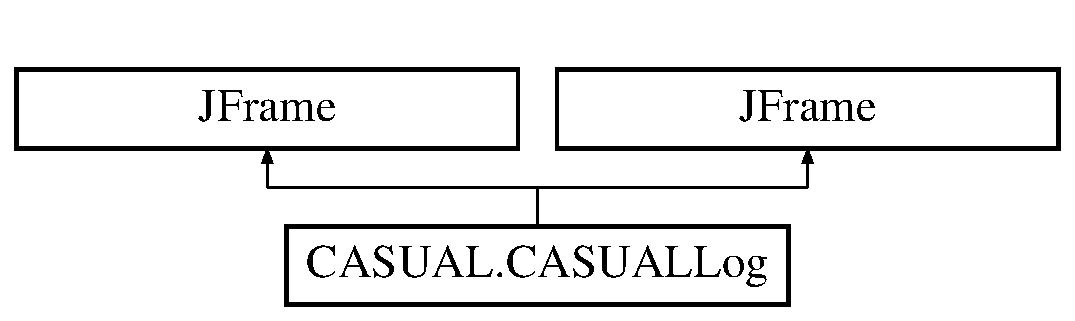
\includegraphics[height=2.000000cm]{classCASUAL_1_1CASUALLog}
\end{center}
\end{figure}
\subsection*{Public Member Functions}
\begin{DoxyCompactItemize}
\item 
\hyperlink{classCASUAL_1_1CASUALLog_a0bcbd377259e114aa031876b0f5a7419}{C\-A\-S\-U\-A\-L\-Log} ()
\item 
\hyperlink{classCASUAL_1_1CASUALLog_a0bcbd377259e114aa031876b0f5a7419}{C\-A\-S\-U\-A\-L\-Log} ()
\end{DoxyCompactItemize}
\subsection*{Static Public Member Functions}
\begin{DoxyCompactItemize}
\item 
\hypertarget{classCASUAL_1_1CASUALLog_a5325dec9b72cc8c9634d9e4eea19863c}{static void {\bfseries initialize\-As\-Main} ()}\label{classCASUAL_1_1CASUALLog_a5325dec9b72cc8c9634d9e4eea19863c}

\item 
\hypertarget{classCASUAL_1_1CASUALLog_a5325dec9b72cc8c9634d9e4eea19863c}{static void {\bfseries initialize\-As\-Main} ()}\label{classCASUAL_1_1CASUALLog_a5325dec9b72cc8c9634d9e4eea19863c}

\end{DoxyCompactItemize}


\subsection{Detailed Description}
\begin{DoxyAuthor}{Author}
Adam Outler \href{mailto:adamoutler@gmail.com}{\tt adamoutler@gmail.\-com} 
\end{DoxyAuthor}


\subsection{Constructor \& Destructor Documentation}
\hypertarget{classCASUAL_1_1CASUALLog_a0bcbd377259e114aa031876b0f5a7419}{\index{C\-A\-S\-U\-A\-L\-::\-C\-A\-S\-U\-A\-L\-Log@{C\-A\-S\-U\-A\-L\-::\-C\-A\-S\-U\-A\-L\-Log}!C\-A\-S\-U\-A\-L\-Log@{C\-A\-S\-U\-A\-L\-Log}}
\index{C\-A\-S\-U\-A\-L\-Log@{C\-A\-S\-U\-A\-L\-Log}!CASUAL::CASUALLog@{C\-A\-S\-U\-A\-L\-::\-C\-A\-S\-U\-A\-L\-Log}}
\subsubsection[{C\-A\-S\-U\-A\-L\-Log}]{\setlength{\rightskip}{0pt plus 5cm}C\-A\-S\-U\-A\-L.\-C\-A\-S\-U\-A\-L\-Log.\-C\-A\-S\-U\-A\-L\-Log (
\begin{DoxyParamCaption}
{}
\end{DoxyParamCaption}
)}}\label{classCASUAL_1_1CASUALLog_a0bcbd377259e114aa031876b0f5a7419}
Creates new form C\-A\-S\-U\-A\-L\-Log\-J\-Frame \hypertarget{classCASUAL_1_1CASUALLog_a0bcbd377259e114aa031876b0f5a7419}{\index{C\-A\-S\-U\-A\-L\-::\-C\-A\-S\-U\-A\-L\-Log@{C\-A\-S\-U\-A\-L\-::\-C\-A\-S\-U\-A\-L\-Log}!C\-A\-S\-U\-A\-L\-Log@{C\-A\-S\-U\-A\-L\-Log}}
\index{C\-A\-S\-U\-A\-L\-Log@{C\-A\-S\-U\-A\-L\-Log}!CASUAL::CASUALLog@{C\-A\-S\-U\-A\-L\-::\-C\-A\-S\-U\-A\-L\-Log}}
\subsubsection[{C\-A\-S\-U\-A\-L\-Log}]{\setlength{\rightskip}{0pt plus 5cm}C\-A\-S\-U\-A\-L.\-C\-A\-S\-U\-A\-L\-Log.\-C\-A\-S\-U\-A\-L\-Log (
\begin{DoxyParamCaption}
{}
\end{DoxyParamCaption}
)}}\label{classCASUAL_1_1CASUALLog_a0bcbd377259e114aa031876b0f5a7419}
Creates new form C\-A\-S\-U\-A\-L\-Log\-J\-Frame 

The documentation for this class was generated from the following files\-:\begin{DoxyCompactItemize}
\item 
branches/\-C\-A\-S\-U\-A\-L-\/\-Headless/\-G\-U\-I/src/\-C\-A\-S\-U\-A\-L/C\-A\-S\-U\-A\-L\-Log.\-java\item 
branches/\-Testing\-Branch/\-G\-Doc/src/\-C\-A\-S\-U\-A\-L/C\-A\-S\-U\-A\-L\-Log.\-java\end{DoxyCompactItemize}

\hypertarget{classCASUAL_1_1CASUALMain}{\section{C\-A\-S\-U\-A\-L.\-C\-A\-S\-U\-A\-L\-Main Class Reference}
\label{classCASUAL_1_1CASUALMain}\index{C\-A\-S\-U\-A\-L.\-C\-A\-S\-U\-A\-L\-Main@{C\-A\-S\-U\-A\-L.\-C\-A\-S\-U\-A\-L\-Main}}
}
\subsection*{Public Member Functions}
\begin{DoxyCompactItemize}
\item 
void \hyperlink{classCASUAL_1_1CASUALMain_a4a2c70ccb1efe2a01ce8b11aeeea947d}{startup} (String\mbox{[}$\,$\mbox{]} args)
\item 
\hypertarget{classCASUAL_1_1CASUALMain_abf4fa23d2d684f022c04ae4c37d7e19e}{Thread {\bfseries start\-A\-D\-B} ()}\label{classCASUAL_1_1CASUALMain_abf4fa23d2d684f022c04ae4c37d7e19e}

\item 
\hypertarget{classCASUAL_1_1CASUALMain_af8cb23fc7509a733dca74ee4787c5335}{void {\bfseries prepare\-Caspac} ()}\label{classCASUAL_1_1CASUALMain_af8cb23fc7509a733dca74ee4787c5335}

\end{DoxyCompactItemize}
\subsection*{Static Public Member Functions}
\begin{DoxyCompactItemize}
\item 
static void \hyperlink{classCASUAL_1_1CASUALMain_a2d7f82ff2961d36d125005f65fdbcf0e}{main} (String\mbox{[}$\,$\mbox{]} args)
\item 
static void \hyperlink{classCASUAL_1_1CASUALMain_a900f3a8c404f68d18d429a8b5ddc249a}{begin\-C\-A\-S\-U\-A\-L} (String\mbox{[}$\,$\mbox{]} args)
\item 
static void \hyperlink{classCASUAL_1_1CASUALMain_aa8a10751e1501b7e2d9146554e4df252}{shutdown} (int i)
\end{DoxyCompactItemize}
\subsection*{Public Attributes}
\begin{DoxyCompactItemize}
\item 
Runnable \hyperlink{classCASUAL_1_1CASUALMain_ac0104001f09bb1d16dea21e6146abb76}{setup\-C\-A\-S\-U\-A\-L\-C\-A\-S\-P\-A\-C}
\end{DoxyCompactItemize}
\subsection*{Static Public Attributes}
\begin{DoxyCompactItemize}
\item 
final static String \hyperlink{classCASUAL_1_1CASUALMain_a388333cdd95aadbbee46efc43efea098}{default\-Package} = \char`\"{}Test\-Script\char`\"{}
\end{DoxyCompactItemize}


\subsection{Detailed Description}
\begin{DoxyAuthor}{Author}
adam 
\end{DoxyAuthor}


\subsection{Member Function Documentation}
\hypertarget{classCASUAL_1_1CASUALMain_a900f3a8c404f68d18d429a8b5ddc249a}{\index{C\-A\-S\-U\-A\-L\-::\-C\-A\-S\-U\-A\-L\-Main@{C\-A\-S\-U\-A\-L\-::\-C\-A\-S\-U\-A\-L\-Main}!begin\-C\-A\-S\-U\-A\-L@{begin\-C\-A\-S\-U\-A\-L}}
\index{begin\-C\-A\-S\-U\-A\-L@{begin\-C\-A\-S\-U\-A\-L}!CASUAL::CASUALMain@{C\-A\-S\-U\-A\-L\-::\-C\-A\-S\-U\-A\-L\-Main}}
\subsubsection[{begin\-C\-A\-S\-U\-A\-L}]{\setlength{\rightskip}{0pt plus 5cm}static void C\-A\-S\-U\-A\-L.\-C\-A\-S\-U\-A\-L\-Main.\-begin\-C\-A\-S\-U\-A\-L (
\begin{DoxyParamCaption}
\item[{String\mbox{[}$\,$\mbox{]}}]{args}
\end{DoxyParamCaption}
)\hspace{0.3cm}{\ttfamily [static]}}}\label{classCASUAL_1_1CASUALMain_a900f3a8c404f68d18d429a8b5ddc249a}
Begins actual \hyperlink{namespaceCASUAL}{C\-A\-S\-U\-A\-L} modes this can be called as a reset for \hyperlink{namespaceCASUAL}{C\-A\-S\-U\-A\-L} without losing args\mbox{[}\mbox{]} in case of a problem


\begin{DoxyParams}{Parameters}
{\em args} & \\
\hline
\end{DoxyParams}
\hypertarget{classCASUAL_1_1CASUALMain_a2d7f82ff2961d36d125005f65fdbcf0e}{\index{C\-A\-S\-U\-A\-L\-::\-C\-A\-S\-U\-A\-L\-Main@{C\-A\-S\-U\-A\-L\-::\-C\-A\-S\-U\-A\-L\-Main}!main@{main}}
\index{main@{main}!CASUAL::CASUALMain@{C\-A\-S\-U\-A\-L\-::\-C\-A\-S\-U\-A\-L\-Main}}
\subsubsection[{main}]{\setlength{\rightskip}{0pt plus 5cm}static void C\-A\-S\-U\-A\-L.\-C\-A\-S\-U\-A\-L\-Main.\-main (
\begin{DoxyParamCaption}
\item[{String\mbox{[}$\,$\mbox{]}}]{args}
\end{DoxyParamCaption}
)\hspace{0.3cm}{\ttfamily [static]}}}\label{classCASUAL_1_1CASUALMain_a2d7f82ff2961d36d125005f65fdbcf0e}
Main method launching the application.


\begin{DoxyParams}{Parameters}
{\em args} & \\
\hline
\end{DoxyParams}
\hypertarget{classCASUAL_1_1CASUALMain_aa8a10751e1501b7e2d9146554e4df252}{\index{C\-A\-S\-U\-A\-L\-::\-C\-A\-S\-U\-A\-L\-Main@{C\-A\-S\-U\-A\-L\-::\-C\-A\-S\-U\-A\-L\-Main}!shutdown@{shutdown}}
\index{shutdown@{shutdown}!CASUAL::CASUALMain@{C\-A\-S\-U\-A\-L\-::\-C\-A\-S\-U\-A\-L\-Main}}
\subsubsection[{shutdown}]{\setlength{\rightskip}{0pt plus 5cm}static void C\-A\-S\-U\-A\-L.\-C\-A\-S\-U\-A\-L\-Main.\-shutdown (
\begin{DoxyParamCaption}
\item[{int}]{i}
\end{DoxyParamCaption}
)\hspace{0.3cm}{\ttfamily [static]}}}\label{classCASUAL_1_1CASUALMain_aa8a10751e1501b7e2d9146554e4df252}
shuts down \hyperlink{namespaceCASUAL}{C\-A\-S\-U\-A\-L}


\begin{DoxyParams}{Parameters}
{\em i} & code to throw \\
\hline
\end{DoxyParams}
\hypertarget{classCASUAL_1_1CASUALMain_a4a2c70ccb1efe2a01ce8b11aeeea947d}{\index{C\-A\-S\-U\-A\-L\-::\-C\-A\-S\-U\-A\-L\-Main@{C\-A\-S\-U\-A\-L\-::\-C\-A\-S\-U\-A\-L\-Main}!startup@{startup}}
\index{startup@{startup}!CASUAL::CASUALMain@{C\-A\-S\-U\-A\-L\-::\-C\-A\-S\-U\-A\-L\-Main}}
\subsubsection[{startup}]{\setlength{\rightskip}{0pt plus 5cm}void C\-A\-S\-U\-A\-L.\-C\-A\-S\-U\-A\-L\-Main.\-startup (
\begin{DoxyParamCaption}
\item[{String\mbox{[}$\,$\mbox{]}}]{args}
\end{DoxyParamCaption}
)}}\label{classCASUAL_1_1CASUALMain_a4a2c70ccb1efe2a01ce8b11aeeea947d}
startup is where \hyperlink{namespaceCASUAL}{C\-A\-S\-U\-A\-L} starts its normal routines for both


\begin{DoxyParams}{Parameters}
{\em args} & commmand line args \\
\hline
\end{DoxyParams}


\subsection{Member Data Documentation}
\hypertarget{classCASUAL_1_1CASUALMain_a388333cdd95aadbbee46efc43efea098}{\index{C\-A\-S\-U\-A\-L\-::\-C\-A\-S\-U\-A\-L\-Main@{C\-A\-S\-U\-A\-L\-::\-C\-A\-S\-U\-A\-L\-Main}!default\-Package@{default\-Package}}
\index{default\-Package@{default\-Package}!CASUAL::CASUALMain@{C\-A\-S\-U\-A\-L\-::\-C\-A\-S\-U\-A\-L\-Main}}
\subsubsection[{default\-Package}]{\setlength{\rightskip}{0pt plus 5cm}final static String C\-A\-S\-U\-A\-L.\-C\-A\-S\-U\-A\-L\-Main.\-default\-Package = \char`\"{}Test\-Script\char`\"{}\hspace{0.3cm}{\ttfamily [static]}}}\label{classCASUAL_1_1CASUALMain_a388333cdd95aadbbee46efc43efea098}
the default package used for I\-D\-E mode or if no scripts are found \hypertarget{classCASUAL_1_1CASUALMain_ac0104001f09bb1d16dea21e6146abb76}{\index{C\-A\-S\-U\-A\-L\-::\-C\-A\-S\-U\-A\-L\-Main@{C\-A\-S\-U\-A\-L\-::\-C\-A\-S\-U\-A\-L\-Main}!setup\-C\-A\-S\-U\-A\-L\-C\-A\-S\-P\-A\-C@{setup\-C\-A\-S\-U\-A\-L\-C\-A\-S\-P\-A\-C}}
\index{setup\-C\-A\-S\-U\-A\-L\-C\-A\-S\-P\-A\-C@{setup\-C\-A\-S\-U\-A\-L\-C\-A\-S\-P\-A\-C}!CASUAL::CASUALMain@{C\-A\-S\-U\-A\-L\-::\-C\-A\-S\-U\-A\-L\-Main}}
\subsubsection[{setup\-C\-A\-S\-U\-A\-L\-C\-A\-S\-P\-A\-C}]{\setlength{\rightskip}{0pt plus 5cm}Runnable C\-A\-S\-U\-A\-L.\-C\-A\-S\-U\-A\-L\-Main.\-setup\-C\-A\-S\-U\-A\-L\-C\-A\-S\-P\-A\-C}}\label{classCASUAL_1_1CASUALMain_ac0104001f09bb1d16dea21e6146abb76}
Scans /\-S\-C\-R\-I\-P\-T\-S/ Folder to locate scripts. 

The documentation for this class was generated from the following file\-:\begin{DoxyCompactItemize}
\item 
trunk/\-C\-A\-S\-U\-A\-Lcore/src/\-C\-A\-S\-U\-A\-L/C\-A\-S\-U\-A\-L\-Main.\-java\end{DoxyCompactItemize}

\hypertarget{classCASUAL_1_1CASUALMessageObject}{\section{C\-A\-S\-U\-A\-L.\-C\-A\-S\-U\-A\-L\-Message\-Object Class Reference}
\label{classCASUAL_1_1CASUALMessageObject}\index{C\-A\-S\-U\-A\-L.\-C\-A\-S\-U\-A\-L\-Message\-Object@{C\-A\-S\-U\-A\-L.\-C\-A\-S\-U\-A\-L\-Message\-Object}}
}
\subsection*{Public Member Functions}
\begin{DoxyCompactItemize}
\item 
\hyperlink{classCASUAL_1_1CASUALMessageObject_ae826dde1386a7040749cc429e40400b5}{C\-A\-S\-U\-A\-L\-Message\-Object} (String message\-Input)
\item 
\hyperlink{classCASUAL_1_1CASUALMessageObject_a92b199db10f96ecbc9be1b26344e82b6}{C\-A\-S\-U\-A\-L\-Message\-Object} (String title, String message\-Input)
\item 
int \hyperlink{classCASUAL_1_1CASUALMessageObject_a7f6babfe3c0458a49081c12b31593e11}{show\-Timeout\-Dialog} (final int P\-R\-E\-S\-E\-T\-\_\-\-T\-I\-M\-E, Component parent\-Component, int option\-Type, int time\-Out\-Message\-Type, Object\mbox{[}$\,$\mbox{]} options, final Object initial\-Value)
\item 
String \hyperlink{classCASUAL_1_1CASUALMessageObject_a044a50f100490ac815197597bc2b0cc3}{input\-Dialog} ()  throws Headless\-Exception 
\item 
int \hyperlink{classCASUAL_1_1CASUALMessageObject_a94d3197760f77cdbd6b60fbf874976bc}{show\-Action\-Required\-Dialog} ()  throws Headless\-Exception 
\item 
int \hyperlink{classCASUAL_1_1CASUALMessageObject_acacbc59bd2fcd53f7746d8e8966377a5}{show\-User\-Cancel\-Option} ()
\item 
void \hyperlink{classCASUAL_1_1CASUALMessageObject_af1731a686ae654acc68823c3249bbd1c}{show\-Command\-Notification} ()  throws Headless\-Exception 
\item 
void \hyperlink{classCASUAL_1_1CASUALMessageObject_a10b91cd75cc6620e93b546d19cbcf995}{show\-User\-Notification} ()  throws Headless\-Exception 
\item 
void \hyperlink{classCASUAL_1_1CASUALMessageObject_abf3fa13e8cf477d6e74bd1c7846e04c9}{show\-Information\-Message} ()  throws Headless\-Exception 
\item 
void \hyperlink{classCASUAL_1_1CASUALMessageObject_aefd0003f0c1f298da3f5af1107384d2c}{show\-Error\-Dialog} ()  throws Headless\-Exception 
\item 
boolean \hyperlink{classCASUAL_1_1CASUALMessageObject_a1c209c028596425d20c826173586222c}{show\-Yes\-No\-Option} ()
\end{DoxyCompactItemize}
\subsection*{Public Attributes}
\begin{DoxyCompactItemize}
\item 
\hypertarget{classCASUAL_1_1CASUALMessageObject_a9716079f17fbab4b81420fb28be1b3d0}{String {\bfseries original\-Message} = \char`\"{}\char`\"{}}\label{classCASUAL_1_1CASUALMessageObject_a9716079f17fbab4b81420fb28be1b3d0}

\item 
\hypertarget{classCASUAL_1_1CASUALMessageObject_a3ecbe3ab3a844982f085d4e45c3cf66f}{String {\bfseries expected\-Return} = \char`\"{}\char`\"{}}\label{classCASUAL_1_1CASUALMessageObject_a3ecbe3ab3a844982f085d4e45c3cf66f}

\item 
\hypertarget{classCASUAL_1_1CASUALMessageObject_aa05172adf910fdff74387ea7e8a1c03f}{String {\bfseries title}}\label{classCASUAL_1_1CASUALMessageObject_aa05172adf910fdff74387ea7e8a1c03f}

\item 
\hypertarget{classCASUAL_1_1CASUALMessageObject_a39eaae2b27f09933cfeb9089499fede6}{String {\bfseries message\-Text}}\label{classCASUAL_1_1CASUALMessageObject_a39eaae2b27f09933cfeb9089499fede6}

\item 
\hypertarget{classCASUAL_1_1CASUALMessageObject_a782918a5c0887c7d784d965296012b78}{int {\bfseries message\-Type}}\label{classCASUAL_1_1CASUALMessageObject_a782918a5c0887c7d784d965296012b78}

\item 
\hypertarget{classCASUAL_1_1CASUALMessageObject_ad62eac89e98a77dab14408d4d2cf03b5}{String {\bfseries message}}\label{classCASUAL_1_1CASUALMessageObject_ad62eac89e98a77dab14408d4d2cf03b5}

\item 
\hypertarget{classCASUAL_1_1CASUALMessageObject_af046b1b60b9c4a847bddd8f0a6b112be}{int {\bfseries timeout\-Option\-Type}}\label{classCASUAL_1_1CASUALMessageObject_af046b1b60b9c4a847bddd8f0a6b112be}

\item 
\hypertarget{classCASUAL_1_1CASUALMessageObject_aadff4442c0e9beed9b99144efb9a99f8}{Object {\bfseries timeout\-Initial\-Value}}\label{classCASUAL_1_1CASUALMessageObject_aadff4442c0e9beed9b99144efb9a99f8}

\item 
\hypertarget{classCASUAL_1_1CASUALMessageObject_aba5217eefa6ca75bb6ccc24f70467d9a}{Object\mbox{[}$\,$\mbox{]} {\bfseries timeout\-Options}}\label{classCASUAL_1_1CASUALMessageObject_aba5217eefa6ca75bb6ccc24f70467d9a}

\item 
\hypertarget{classCASUAL_1_1CASUALMessageObject_a87012881239a6672883c8a08cbadb52e}{int {\bfseries timeout\-Preset\-Time}}\label{classCASUAL_1_1CASUALMessageObject_a87012881239a6672883c8a08cbadb52e}

\item 
\hypertarget{classCASUAL_1_1CASUALMessageObject_a6d7381fc02cd0fa6268f445eaf25f7cb}{int {\bfseries timeout\-Message\-Type}}\label{classCASUAL_1_1CASUALMessageObject_a6d7381fc02cd0fa6268f445eaf25f7cb}

\end{DoxyCompactItemize}


\subsection{Detailed Description}
\begin{DoxyAuthor}{Author}
adam 
\end{DoxyAuthor}


\subsection{Constructor \& Destructor Documentation}
\hypertarget{classCASUAL_1_1CASUALMessageObject_ae826dde1386a7040749cc429e40400b5}{\index{C\-A\-S\-U\-A\-L\-::\-C\-A\-S\-U\-A\-L\-Message\-Object@{C\-A\-S\-U\-A\-L\-::\-C\-A\-S\-U\-A\-L\-Message\-Object}!C\-A\-S\-U\-A\-L\-Message\-Object@{C\-A\-S\-U\-A\-L\-Message\-Object}}
\index{C\-A\-S\-U\-A\-L\-Message\-Object@{C\-A\-S\-U\-A\-L\-Message\-Object}!CASUAL::CASUALMessageObject@{C\-A\-S\-U\-A\-L\-::\-C\-A\-S\-U\-A\-L\-Message\-Object}}
\subsubsection[{C\-A\-S\-U\-A\-L\-Message\-Object}]{\setlength{\rightskip}{0pt plus 5cm}C\-A\-S\-U\-A\-L.\-C\-A\-S\-U\-A\-L\-Message\-Object.\-C\-A\-S\-U\-A\-L\-Message\-Object (
\begin{DoxyParamCaption}
\item[{String}]{message\-Input}
\end{DoxyParamCaption}
)}}\label{classCASUAL_1_1CASUALMessageObject_ae826dde1386a7040749cc429e40400b5}
instantiates an interaction


\begin{DoxyParams}{Parameters}
{\em message\-Input} & can be title,message or title$>$$>$$>$message, or just message and title will be automatically chosen \\
\hline
\end{DoxyParams}
\hypertarget{classCASUAL_1_1CASUALMessageObject_a92b199db10f96ecbc9be1b26344e82b6}{\index{C\-A\-S\-U\-A\-L\-::\-C\-A\-S\-U\-A\-L\-Message\-Object@{C\-A\-S\-U\-A\-L\-::\-C\-A\-S\-U\-A\-L\-Message\-Object}!C\-A\-S\-U\-A\-L\-Message\-Object@{C\-A\-S\-U\-A\-L\-Message\-Object}}
\index{C\-A\-S\-U\-A\-L\-Message\-Object@{C\-A\-S\-U\-A\-L\-Message\-Object}!CASUAL::CASUALMessageObject@{C\-A\-S\-U\-A\-L\-::\-C\-A\-S\-U\-A\-L\-Message\-Object}}
\subsubsection[{C\-A\-S\-U\-A\-L\-Message\-Object}]{\setlength{\rightskip}{0pt plus 5cm}C\-A\-S\-U\-A\-L.\-C\-A\-S\-U\-A\-L\-Message\-Object.\-C\-A\-S\-U\-A\-L\-Message\-Object (
\begin{DoxyParamCaption}
\item[{String}]{title, }
\item[{String}]{message\-Input}
\end{DoxyParamCaption}
)}}\label{classCASUAL_1_1CASUALMessageObject_a92b199db10f96ecbc9be1b26344e82b6}
instantiates a C\-A\-S\-U\-A\-L\-Interaction


\begin{DoxyParams}{Parameters}
{\em title} & title to display on interaction \\
\hline
{\em message\-Input} & message to display on interaction \\
\hline
\end{DoxyParams}


\subsection{Member Function Documentation}
\hypertarget{classCASUAL_1_1CASUALMessageObject_a044a50f100490ac815197597bc2b0cc3}{\index{C\-A\-S\-U\-A\-L\-::\-C\-A\-S\-U\-A\-L\-Message\-Object@{C\-A\-S\-U\-A\-L\-::\-C\-A\-S\-U\-A\-L\-Message\-Object}!input\-Dialog@{input\-Dialog}}
\index{input\-Dialog@{input\-Dialog}!CASUAL::CASUALMessageObject@{C\-A\-S\-U\-A\-L\-::\-C\-A\-S\-U\-A\-L\-Message\-Object}}
\subsubsection[{input\-Dialog}]{\setlength{\rightskip}{0pt plus 5cm}String C\-A\-S\-U\-A\-L.\-C\-A\-S\-U\-A\-L\-Message\-Object.\-input\-Dialog (
\begin{DoxyParamCaption}
{}
\end{DoxyParamCaption}
) throws Headless\-Exception}}\label{classCASUAL_1_1CASUALMessageObject_a044a50f100490ac815197597bc2b0cc3}
shows an input dialog

\begin{DoxyReturn}{Returns}
value from user input 
\end{DoxyReturn}

\begin{DoxyExceptions}{Exceptions}
{\em Headless\-Exception} & \\
\hline
\end{DoxyExceptions}
\hypertarget{classCASUAL_1_1CASUALMessageObject_a94d3197760f77cdbd6b60fbf874976bc}{\index{C\-A\-S\-U\-A\-L\-::\-C\-A\-S\-U\-A\-L\-Message\-Object@{C\-A\-S\-U\-A\-L\-::\-C\-A\-S\-U\-A\-L\-Message\-Object}!show\-Action\-Required\-Dialog@{show\-Action\-Required\-Dialog}}
\index{show\-Action\-Required\-Dialog@{show\-Action\-Required\-Dialog}!CASUAL::CASUALMessageObject@{C\-A\-S\-U\-A\-L\-::\-C\-A\-S\-U\-A\-L\-Message\-Object}}
\subsubsection[{show\-Action\-Required\-Dialog}]{\setlength{\rightskip}{0pt plus 5cm}int C\-A\-S\-U\-A\-L.\-C\-A\-S\-U\-A\-L\-Message\-Object.\-show\-Action\-Required\-Dialog (
\begin{DoxyParamCaption}
{}
\end{DoxyParamCaption}
) throws Headless\-Exception}}\label{classCASUAL_1_1CASUALMessageObject_a94d3197760f77cdbd6b60fbf874976bc}
shows action required dialog

\begin{DoxyReturn}{Returns}
1 if user didn't do it, or 0 if user did it. 
\end{DoxyReturn}

\begin{DoxyExceptions}{Exceptions}
{\em Headless\-Exception} & \\
\hline
\end{DoxyExceptions}
\hypertarget{classCASUAL_1_1CASUALMessageObject_af1731a686ae654acc68823c3249bbd1c}{\index{C\-A\-S\-U\-A\-L\-::\-C\-A\-S\-U\-A\-L\-Message\-Object@{C\-A\-S\-U\-A\-L\-::\-C\-A\-S\-U\-A\-L\-Message\-Object}!show\-Command\-Notification@{show\-Command\-Notification}}
\index{show\-Command\-Notification@{show\-Command\-Notification}!CASUAL::CASUALMessageObject@{C\-A\-S\-U\-A\-L\-::\-C\-A\-S\-U\-A\-L\-Message\-Object}}
\subsubsection[{show\-Command\-Notification}]{\setlength{\rightskip}{0pt plus 5cm}void C\-A\-S\-U\-A\-L.\-C\-A\-S\-U\-A\-L\-Message\-Object.\-show\-Command\-Notification (
\begin{DoxyParamCaption}
{}
\end{DoxyParamCaption}
) throws Headless\-Exception}}\label{classCASUAL_1_1CASUALMessageObject_af1731a686ae654acc68823c3249bbd1c}
displays command notification


\begin{DoxyExceptions}{Exceptions}
{\em Headless\-Exception} & \\
\hline
\end{DoxyExceptions}
\hypertarget{classCASUAL_1_1CASUALMessageObject_aefd0003f0c1f298da3f5af1107384d2c}{\index{C\-A\-S\-U\-A\-L\-::\-C\-A\-S\-U\-A\-L\-Message\-Object@{C\-A\-S\-U\-A\-L\-::\-C\-A\-S\-U\-A\-L\-Message\-Object}!show\-Error\-Dialog@{show\-Error\-Dialog}}
\index{show\-Error\-Dialog@{show\-Error\-Dialog}!CASUAL::CASUALMessageObject@{C\-A\-S\-U\-A\-L\-::\-C\-A\-S\-U\-A\-L\-Message\-Object}}
\subsubsection[{show\-Error\-Dialog}]{\setlength{\rightskip}{0pt plus 5cm}void C\-A\-S\-U\-A\-L.\-C\-A\-S\-U\-A\-L\-Message\-Object.\-show\-Error\-Dialog (
\begin{DoxyParamCaption}
{}
\end{DoxyParamCaption}
) throws Headless\-Exception}}\label{classCASUAL_1_1CASUALMessageObject_aefd0003f0c1f298da3f5af1107384d2c}
displays error message


\begin{DoxyExceptions}{Exceptions}
{\em Headless\-Exception} & \\
\hline
\end{DoxyExceptions}
\hypertarget{classCASUAL_1_1CASUALMessageObject_abf3fa13e8cf477d6e74bd1c7846e04c9}{\index{C\-A\-S\-U\-A\-L\-::\-C\-A\-S\-U\-A\-L\-Message\-Object@{C\-A\-S\-U\-A\-L\-::\-C\-A\-S\-U\-A\-L\-Message\-Object}!show\-Information\-Message@{show\-Information\-Message}}
\index{show\-Information\-Message@{show\-Information\-Message}!CASUAL::CASUALMessageObject@{C\-A\-S\-U\-A\-L\-::\-C\-A\-S\-U\-A\-L\-Message\-Object}}
\subsubsection[{show\-Information\-Message}]{\setlength{\rightskip}{0pt plus 5cm}void C\-A\-S\-U\-A\-L.\-C\-A\-S\-U\-A\-L\-Message\-Object.\-show\-Information\-Message (
\begin{DoxyParamCaption}
{}
\end{DoxyParamCaption}
) throws Headless\-Exception}}\label{classCASUAL_1_1CASUALMessageObject_abf3fa13e8cf477d6e74bd1c7846e04c9}
displays information message


\begin{DoxyExceptions}{Exceptions}
{\em Headless\-Exception} & \\
\hline
\end{DoxyExceptions}
\hypertarget{classCASUAL_1_1CASUALMessageObject_a7f6babfe3c0458a49081c12b31593e11}{\index{C\-A\-S\-U\-A\-L\-::\-C\-A\-S\-U\-A\-L\-Message\-Object@{C\-A\-S\-U\-A\-L\-::\-C\-A\-S\-U\-A\-L\-Message\-Object}!show\-Timeout\-Dialog@{show\-Timeout\-Dialog}}
\index{show\-Timeout\-Dialog@{show\-Timeout\-Dialog}!CASUAL::CASUALMessageObject@{C\-A\-S\-U\-A\-L\-::\-C\-A\-S\-U\-A\-L\-Message\-Object}}
\subsubsection[{show\-Timeout\-Dialog}]{\setlength{\rightskip}{0pt plus 5cm}int C\-A\-S\-U\-A\-L.\-C\-A\-S\-U\-A\-L\-Message\-Object.\-show\-Timeout\-Dialog (
\begin{DoxyParamCaption}
\item[{final int}]{P\-R\-E\-S\-E\-T\-\_\-\-T\-I\-M\-E, }
\item[{Component}]{parent\-Component, }
\item[{int}]{option\-Type, }
\item[{int}]{time\-Out\-Message\-Type, }
\item[{Object\mbox{[}$\,$\mbox{]}}]{options, }
\item[{final Object}]{initial\-Value}
\end{DoxyParamCaption}
)}}\label{classCASUAL_1_1CASUALMessageObject_a7f6babfe3c0458a49081c12b31593e11}
C\-A\-S\-U\-A\-L\-Interaction input device shows a Time\-Out\-Dialog


\begin{DoxyParams}{Parameters}
{\em P\-R\-E\-S\-E\-T\-\_\-\-T\-I\-M\-E} & time to show message \\
\hline
{\em parent\-Component} & where to hover over \\
\hline
{\em option\-Type} & j\-Option\-Pane.\-O\-P\-T\-I\-O\-N\-\_\- \\
\hline
{\em time\-Out\-Message\-Type} & j\-Option\-Pane.\-M\-E\-S\-S\-A\-G\-E\-T\-Y\-P\-E \\
\hline
{\em options} & array of options \\
\hline
{\em initial\-Value} & value to choose if none other are chosen \\
\hline
\end{DoxyParams}
\begin{DoxyReturn}{Returns}
value chosen 0 for first, 1 for second... 
\end{DoxyReturn}
\hypertarget{classCASUAL_1_1CASUALMessageObject_acacbc59bd2fcd53f7746d8e8966377a5}{\index{C\-A\-S\-U\-A\-L\-::\-C\-A\-S\-U\-A\-L\-Message\-Object@{C\-A\-S\-U\-A\-L\-::\-C\-A\-S\-U\-A\-L\-Message\-Object}!show\-User\-Cancel\-Option@{show\-User\-Cancel\-Option}}
\index{show\-User\-Cancel\-Option@{show\-User\-Cancel\-Option}!CASUAL::CASUALMessageObject@{C\-A\-S\-U\-A\-L\-::\-C\-A\-S\-U\-A\-L\-Message\-Object}}
\subsubsection[{show\-User\-Cancel\-Option}]{\setlength{\rightskip}{0pt plus 5cm}int C\-A\-S\-U\-A\-L.\-C\-A\-S\-U\-A\-L\-Message\-Object.\-show\-User\-Cancel\-Option (
\begin{DoxyParamCaption}
{}
\end{DoxyParamCaption}
)}}\label{classCASUAL_1_1CASUALMessageObject_acacbc59bd2fcd53f7746d8e8966377a5}
displays user cancel option

\begin{DoxyReturn}{Returns}
1 if cancel was requested 
\end{DoxyReturn}
\hypertarget{classCASUAL_1_1CASUALMessageObject_a10b91cd75cc6620e93b546d19cbcf995}{\index{C\-A\-S\-U\-A\-L\-::\-C\-A\-S\-U\-A\-L\-Message\-Object@{C\-A\-S\-U\-A\-L\-::\-C\-A\-S\-U\-A\-L\-Message\-Object}!show\-User\-Notification@{show\-User\-Notification}}
\index{show\-User\-Notification@{show\-User\-Notification}!CASUAL::CASUALMessageObject@{C\-A\-S\-U\-A\-L\-::\-C\-A\-S\-U\-A\-L\-Message\-Object}}
\subsubsection[{show\-User\-Notification}]{\setlength{\rightskip}{0pt plus 5cm}void C\-A\-S\-U\-A\-L.\-C\-A\-S\-U\-A\-L\-Message\-Object.\-show\-User\-Notification (
\begin{DoxyParamCaption}
{}
\end{DoxyParamCaption}
) throws Headless\-Exception}}\label{classCASUAL_1_1CASUALMessageObject_a10b91cd75cc6620e93b546d19cbcf995}
displays user notification


\begin{DoxyExceptions}{Exceptions}
{\em Headless\-Exception} & \\
\hline
\end{DoxyExceptions}
\hypertarget{classCASUAL_1_1CASUALMessageObject_a1c209c028596425d20c826173586222c}{\index{C\-A\-S\-U\-A\-L\-::\-C\-A\-S\-U\-A\-L\-Message\-Object@{C\-A\-S\-U\-A\-L\-::\-C\-A\-S\-U\-A\-L\-Message\-Object}!show\-Yes\-No\-Option@{show\-Yes\-No\-Option}}
\index{show\-Yes\-No\-Option@{show\-Yes\-No\-Option}!CASUAL::CASUALMessageObject@{C\-A\-S\-U\-A\-L\-::\-C\-A\-S\-U\-A\-L\-Message\-Object}}
\subsubsection[{show\-Yes\-No\-Option}]{\setlength{\rightskip}{0pt plus 5cm}boolean C\-A\-S\-U\-A\-L.\-C\-A\-S\-U\-A\-L\-Message\-Object.\-show\-Yes\-No\-Option (
\begin{DoxyParamCaption}
{}
\end{DoxyParamCaption}
)}}\label{classCASUAL_1_1CASUALMessageObject_a1c209c028596425d20c826173586222c}
displays a Yes/\-No dialog

\begin{DoxyReturn}{Returns}
true if yes, false if no 
\end{DoxyReturn}


The documentation for this class was generated from the following file\-:\begin{DoxyCompactItemize}
\item 
trunk/\-C\-A\-S\-U\-A\-Lcore/src/\-C\-A\-S\-U\-A\-L/C\-A\-S\-U\-A\-L\-Message\-Object.\-java\end{DoxyCompactItemize}

\hypertarget{classCASUAL_1_1misc_1_1CASUALScrFilter}{\section{C\-A\-S\-U\-A\-L.\-misc.\-C\-A\-S\-U\-A\-L\-Scr\-Filter Class Reference}
\label{classCASUAL_1_1misc_1_1CASUALScrFilter}\index{C\-A\-S\-U\-A\-L.\-misc.\-C\-A\-S\-U\-A\-L\-Scr\-Filter@{C\-A\-S\-U\-A\-L.\-misc.\-C\-A\-S\-U\-A\-L\-Scr\-Filter}}
}
Inheritance diagram for C\-A\-S\-U\-A\-L.\-misc.\-C\-A\-S\-U\-A\-L\-Scr\-Filter\-:\begin{figure}[H]
\begin{center}
\leavevmode
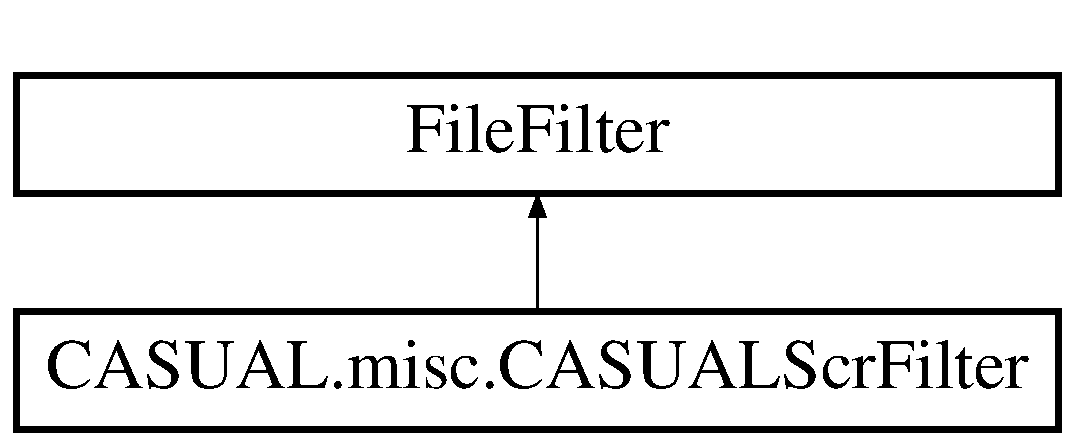
\includegraphics[height=2.000000cm]{classCASUAL_1_1misc_1_1CASUALScrFilter}
\end{center}
\end{figure}
\subsection*{Public Member Functions}
\begin{DoxyCompactItemize}
\item 
boolean \hyperlink{classCASUAL_1_1misc_1_1CASUALScrFilter_ac0849a3d91971a8c385078a046ce91b0}{accept} (File file)
\item 
String \hyperlink{classCASUAL_1_1misc_1_1CASUALScrFilter_abf2196797a290d8b2666468c5ae2e628}{get\-Description} ()
\end{DoxyCompactItemize}


\subsection{Detailed Description}
\begin{DoxyAuthor}{Author}
Jeremy 
\end{DoxyAuthor}


\subsection{Member Function Documentation}
\hypertarget{classCASUAL_1_1misc_1_1CASUALScrFilter_ac0849a3d91971a8c385078a046ce91b0}{\index{C\-A\-S\-U\-A\-L\-::misc\-::\-C\-A\-S\-U\-A\-L\-Scr\-Filter@{C\-A\-S\-U\-A\-L\-::misc\-::\-C\-A\-S\-U\-A\-L\-Scr\-Filter}!accept@{accept}}
\index{accept@{accept}!CASUAL::misc::CASUALScrFilter@{C\-A\-S\-U\-A\-L\-::misc\-::\-C\-A\-S\-U\-A\-L\-Scr\-Filter}}
\subsubsection[{accept}]{\setlength{\rightskip}{0pt plus 5cm}boolean C\-A\-S\-U\-A\-L.\-misc.\-C\-A\-S\-U\-A\-L\-Scr\-Filter.\-accept (
\begin{DoxyParamCaption}
\item[{File}]{file}
\end{DoxyParamCaption}
)}}\label{classCASUAL_1_1misc_1_1CASUALScrFilter_ac0849a3d91971a8c385078a046ce91b0}
chooses only valid script files


\begin{DoxyParams}{Parameters}
{\em file} & file to test \\
\hline
\end{DoxyParams}
\begin{DoxyReturn}{Returns}
true if file is a script 
\end{DoxyReturn}
\hypertarget{classCASUAL_1_1misc_1_1CASUALScrFilter_abf2196797a290d8b2666468c5ae2e628}{\index{C\-A\-S\-U\-A\-L\-::misc\-::\-C\-A\-S\-U\-A\-L\-Scr\-Filter@{C\-A\-S\-U\-A\-L\-::misc\-::\-C\-A\-S\-U\-A\-L\-Scr\-Filter}!get\-Description@{get\-Description}}
\index{get\-Description@{get\-Description}!CASUAL::misc::CASUALScrFilter@{C\-A\-S\-U\-A\-L\-::misc\-::\-C\-A\-S\-U\-A\-L\-Scr\-Filter}}
\subsubsection[{get\-Description}]{\setlength{\rightskip}{0pt plus 5cm}String C\-A\-S\-U\-A\-L.\-misc.\-C\-A\-S\-U\-A\-L\-Scr\-Filter.\-get\-Description (
\begin{DoxyParamCaption}
{}
\end{DoxyParamCaption}
)}}\label{classCASUAL_1_1misc_1_1CASUALScrFilter_abf2196797a290d8b2666468c5ae2e628}
files to be listed

\begin{DoxyReturn}{Returns}
casual scripts only 
\end{DoxyReturn}


The documentation for this class was generated from the following file\-:\begin{DoxyCompactItemize}
\item 
trunk/\-C\-A\-S\-U\-A\-Lcore/src/\-C\-A\-S\-U\-A\-L/misc/C\-A\-S\-U\-A\-L\-Scr\-Filter.\-java\end{DoxyCompactItemize}

\hypertarget{classCASUAL_1_1CASUALScriptParser}{\section{C\-A\-S\-U\-A\-L.\-C\-A\-S\-U\-A\-L\-Script\-Parser Class Reference}
\label{classCASUAL_1_1CASUALScriptParser}\index{C\-A\-S\-U\-A\-L.\-C\-A\-S\-U\-A\-L\-Script\-Parser@{C\-A\-S\-U\-A\-L.\-C\-A\-S\-U\-A\-L\-Script\-Parser}}
}
\subsection*{Public Member Functions}
\begin{DoxyCompactItemize}
\item 
\hypertarget{classCASUAL_1_1CASUALScriptParser_a1cdb36f0abcb04d969cf30be504e9bd9}{void {\bfseries execute\-Selected\-Script\-Resource} (String \hyperlink{classCASUAL_1_1caspac_1_1Script}{Script})}\label{classCASUAL_1_1CASUALScriptParser_a1cdb36f0abcb04d969cf30be504e9bd9}

\item 
\hypertarget{classCASUAL_1_1CASUALScriptParser_a25b767d273a1366373d6a218759d6945}{void {\bfseries execute\-Selected\-Script\-File} (String \hyperlink{classCASUAL_1_1caspac_1_1Script}{Script})}\label{classCASUAL_1_1CASUALScriptParser_a25b767d273a1366373d6a218759d6945}

\item 
\hypertarget{classCASUAL_1_1CASUALScriptParser_ab303a8995ae16b45f465759febc3e461}{void {\bfseries execute\-One\-Shot\-Command} (String Line)}\label{classCASUAL_1_1CASUALScriptParser_ab303a8995ae16b45f465759febc3e461}

\item 
\hypertarget{classCASUAL_1_1CASUALScriptParser_a1cdb36f0abcb04d969cf30be504e9bd9}{void {\bfseries execute\-Selected\-Script\-Resource} (String \hyperlink{classCASUAL_1_1caspac_1_1Script}{Script})}\label{classCASUAL_1_1CASUALScriptParser_a1cdb36f0abcb04d969cf30be504e9bd9}

\item 
\hypertarget{classCASUAL_1_1CASUALScriptParser_a25b767d273a1366373d6a218759d6945}{void {\bfseries execute\-Selected\-Script\-File} (String \hyperlink{classCASUAL_1_1caspac_1_1Script}{Script})}\label{classCASUAL_1_1CASUALScriptParser_a25b767d273a1366373d6a218759d6945}

\item 
\hypertarget{classCASUAL_1_1CASUALScriptParser_ab303a8995ae16b45f465759febc3e461}{void {\bfseries execute\-One\-Shot\-Command} (String Line)}\label{classCASUAL_1_1CASUALScriptParser_ab303a8995ae16b45f465759febc3e461}

\item 
void \hyperlink{classCASUAL_1_1CASUALScriptParser_af3522851b007af1b1e00999bb5b966ba}{load\-File\-And\-Execute} (\hyperlink{classCASUAL_1_1caspac_1_1Caspac}{Caspac} caspac, boolean multi\-Threaded)
\item 
String \hyperlink{classCASUAL_1_1CASUALScriptParser_a05f4f6b1fd11ab2d710a4307f2104754}{execute\-One\-Shot\-Command} (String Line)
\item 
\hypertarget{classCASUAL_1_1CASUALScriptParser_a6cee6a59d0ab94efd5de33b87d80cc48}{void {\bfseries execute\-Selected\-Script} (final \hyperlink{classCASUAL_1_1caspac_1_1Caspac}{Caspac} caspac, boolean start\-Threaded)}\label{classCASUAL_1_1CASUALScriptParser_a6cee6a59d0ab94efd5de33b87d80cc48}

\end{DoxyCompactItemize}


\subsection{Detailed Description}
\begin{DoxyAuthor}{Author}
adam 
\end{DoxyAuthor}


\subsection{Member Function Documentation}
\hypertarget{classCASUAL_1_1CASUALScriptParser_a05f4f6b1fd11ab2d710a4307f2104754}{\index{C\-A\-S\-U\-A\-L\-::\-C\-A\-S\-U\-A\-L\-Script\-Parser@{C\-A\-S\-U\-A\-L\-::\-C\-A\-S\-U\-A\-L\-Script\-Parser}!execute\-One\-Shot\-Command@{execute\-One\-Shot\-Command}}
\index{execute\-One\-Shot\-Command@{execute\-One\-Shot\-Command}!CASUAL::CASUALScriptParser@{C\-A\-S\-U\-A\-L\-::\-C\-A\-S\-U\-A\-L\-Script\-Parser}}
\subsubsection[{execute\-One\-Shot\-Command}]{\setlength{\rightskip}{0pt plus 5cm}String C\-A\-S\-U\-A\-L.\-C\-A\-S\-U\-A\-L\-Script\-Parser.\-execute\-One\-Shot\-Command (
\begin{DoxyParamCaption}
\item[{String}]{Line}
\end{DoxyParamCaption}
)}}\label{classCASUAL_1_1CASUALScriptParser_a05f4f6b1fd11ab2d710a4307f2104754}
provides a way to insert a line of \hyperlink{namespaceCASUAL}{C\-A\-S\-U\-A\-L} script.


\begin{DoxyParams}{Parameters}
{\em Line} & line to execute \\
\hline
\end{DoxyParams}
\begin{DoxyReturn}{Returns}
from \hyperlink{namespaceCASUAL}{C\-A\-S\-U\-A\-L} language 
\end{DoxyReturn}
\hypertarget{classCASUAL_1_1CASUALScriptParser_af3522851b007af1b1e00999bb5b966ba}{\index{C\-A\-S\-U\-A\-L\-::\-C\-A\-S\-U\-A\-L\-Script\-Parser@{C\-A\-S\-U\-A\-L\-::\-C\-A\-S\-U\-A\-L\-Script\-Parser}!load\-File\-And\-Execute@{load\-File\-And\-Execute}}
\index{load\-File\-And\-Execute@{load\-File\-And\-Execute}!CASUAL::CASUALScriptParser@{C\-A\-S\-U\-A\-L\-::\-C\-A\-S\-U\-A\-L\-Script\-Parser}}
\subsubsection[{load\-File\-And\-Execute}]{\setlength{\rightskip}{0pt plus 5cm}void C\-A\-S\-U\-A\-L.\-C\-A\-S\-U\-A\-L\-Script\-Parser.\-load\-File\-And\-Execute (
\begin{DoxyParamCaption}
\item[{{\bf Caspac}}]{caspac, }
\item[{boolean}]{multi\-Threaded}
\end{DoxyParamCaption}
)}}\label{classCASUAL_1_1CASUALScriptParser_af3522851b007af1b1e00999bb5b966ba}
executes a \hyperlink{namespaceCASUAL}{C\-A\-S\-U\-A\-L} script from a file


\begin{DoxyParams}{Parameters}
{\em caspac} & Caspac used for the script \\
\hline
{\em multi\-Threaded} & false executes on main thread \\
\hline
\end{DoxyParams}


The documentation for this class was generated from the following files\-:\begin{DoxyCompactItemize}
\item 
branches/\-C\-A\-S\-U\-A\-L-\/\-Headless/\-G\-U\-I/src/\-C\-A\-S\-U\-A\-L/C\-A\-S\-U\-A\-L\-Script\-Parser.\-java\item 
branches/\-Testing\-Branch/\-G\-Doc/src/\-C\-A\-S\-U\-A\-L/C\-A\-S\-U\-A\-L\-Script\-Parser.\-java\item 
trunk/\-C\-A\-S\-U\-A\-Lcore/src/\-C\-A\-S\-U\-A\-L/C\-A\-S\-U\-A\-L\-Script\-Parser.\-java\end{DoxyCompactItemize}

\hypertarget{classGUI_1_1development_1_1CASUALShowJFrameMessageObject}{\section{G\-U\-I.\-development.\-C\-A\-S\-U\-A\-L\-Show\-J\-Frame\-Message\-Object Class Reference}
\label{classGUI_1_1development_1_1CASUALShowJFrameMessageObject}\index{G\-U\-I.\-development.\-C\-A\-S\-U\-A\-L\-Show\-J\-Frame\-Message\-Object@{G\-U\-I.\-development.\-C\-A\-S\-U\-A\-L\-Show\-J\-Frame\-Message\-Object}}
}
Inheritance diagram for G\-U\-I.\-development.\-C\-A\-S\-U\-A\-L\-Show\-J\-Frame\-Message\-Object\-:\begin{figure}[H]
\begin{center}
\leavevmode
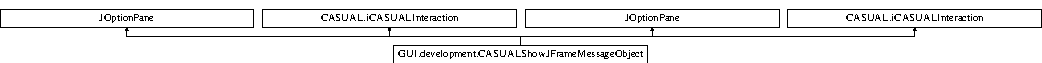
\includegraphics[height=0.845922cm]{classGUI_1_1development_1_1CASUALShowJFrameMessageObject}
\end{center}
\end{figure}
\subsection*{Public Member Functions}
\begin{DoxyCompactItemize}
\item 
String \hyperlink{classGUI_1_1development_1_1CASUALShowJFrameMessageObject_a2ea27451cd76c3c64404413fca107310}{display\-Message} (\hyperlink{classCASUAL_1_1CASUALMessageObject}{C\-A\-S\-U\-A\-L\-Message\-Object} message\-Object)
\item 
\hypertarget{classGUI_1_1development_1_1CASUALShowJFrameMessageObject_a2a1e31b0b8eee95f6023a103f3fca73f}{String {\bfseries get\-Command\-Line\-Input} ()}\label{classGUI_1_1development_1_1CASUALShowJFrameMessageObject_a2a1e31b0b8eee95f6023a103f3fca73f}

\item 
String \hyperlink{classGUI_1_1development_1_1CASUALShowJFrameMessageObject_a2ea27451cd76c3c64404413fca107310}{display\-Message} (\hyperlink{classCASUAL_1_1CASUALMessageObject}{C\-A\-S\-U\-A\-L\-Message\-Object} message\-Object)
\item 
\hypertarget{classGUI_1_1development_1_1CASUALShowJFrameMessageObject_a2a1e31b0b8eee95f6023a103f3fca73f}{String {\bfseries get\-Command\-Line\-Input} ()}\label{classGUI_1_1development_1_1CASUALShowJFrameMessageObject_a2a1e31b0b8eee95f6023a103f3fca73f}

\end{DoxyCompactItemize}
\subsection*{Additional Inherited Members}


\subsection{Detailed Description}
\begin{DoxyAuthor}{Author}
adam 
\end{DoxyAuthor}


\subsection{Member Function Documentation}
\hypertarget{classGUI_1_1development_1_1CASUALShowJFrameMessageObject_a2ea27451cd76c3c64404413fca107310}{\index{G\-U\-I\-::development\-::\-C\-A\-S\-U\-A\-L\-Show\-J\-Frame\-Message\-Object@{G\-U\-I\-::development\-::\-C\-A\-S\-U\-A\-L\-Show\-J\-Frame\-Message\-Object}!display\-Message@{display\-Message}}
\index{display\-Message@{display\-Message}!GUI::development::CASUALShowJFrameMessageObject@{G\-U\-I\-::development\-::\-C\-A\-S\-U\-A\-L\-Show\-J\-Frame\-Message\-Object}}
\subsubsection[{display\-Message}]{\setlength{\rightskip}{0pt plus 5cm}String G\-U\-I.\-development.\-C\-A\-S\-U\-A\-L\-Show\-J\-Frame\-Message\-Object.\-display\-Message (
\begin{DoxyParamCaption}
\item[{{\bf C\-A\-S\-U\-A\-L\-Message\-Object}}]{message\-Object}
\end{DoxyParamCaption}
)}}\label{classGUI_1_1development_1_1CASUALShowJFrameMessageObject_a2ea27451cd76c3c64404413fca107310}
Takes a message object and displays to user. To properly implement this class the display\-Message should, at a minimum handle both C\-A\-S\-U\-A\-L\-Message\-Object.\-title and C\-A\-S\-U\-A\-L\-Message\-Object.\-message\-Text.


\begin{DoxyParams}{Parameters}
{\em message\-Object} & defined by \hyperlink{namespaceCASUAL}{C\-A\-S\-U\-A\-L} \\
\hline
\end{DoxyParams}
\begin{DoxyReturn}{Returns}
string value which must be interpereted 
\end{DoxyReturn}


Implements \hyperlink{interfaceCASUAL_1_1iCASUALInteraction_a8c6697fd276aa8519caff45131c14bf4}{C\-A\-S\-U\-A\-L.\-i\-C\-A\-S\-U\-A\-L\-Interaction}.

\hypertarget{classGUI_1_1development_1_1CASUALShowJFrameMessageObject_a2ea27451cd76c3c64404413fca107310}{\index{G\-U\-I\-::development\-::\-C\-A\-S\-U\-A\-L\-Show\-J\-Frame\-Message\-Object@{G\-U\-I\-::development\-::\-C\-A\-S\-U\-A\-L\-Show\-J\-Frame\-Message\-Object}!display\-Message@{display\-Message}}
\index{display\-Message@{display\-Message}!GUI::development::CASUALShowJFrameMessageObject@{G\-U\-I\-::development\-::\-C\-A\-S\-U\-A\-L\-Show\-J\-Frame\-Message\-Object}}
\subsubsection[{display\-Message}]{\setlength{\rightskip}{0pt plus 5cm}String G\-U\-I.\-development.\-C\-A\-S\-U\-A\-L\-Show\-J\-Frame\-Message\-Object.\-display\-Message (
\begin{DoxyParamCaption}
\item[{{\bf C\-A\-S\-U\-A\-L\-Message\-Object}}]{message\-Object}
\end{DoxyParamCaption}
)}}\label{classGUI_1_1development_1_1CASUALShowJFrameMessageObject_a2ea27451cd76c3c64404413fca107310}
Takes a message object and displays to user. To properly implement this class the display\-Message should, at a minimum handle both C\-A\-S\-U\-A\-L\-Message\-Object.\-title and C\-A\-S\-U\-A\-L\-Message\-Object.\-message\-Text.


\begin{DoxyParams}{Parameters}
{\em message\-Object} & defined by \hyperlink{namespaceCASUAL}{C\-A\-S\-U\-A\-L} \\
\hline
\end{DoxyParams}
\begin{DoxyReturn}{Returns}
string value which must be interpereted 
\end{DoxyReturn}


Implements \hyperlink{interfaceCASUAL_1_1iCASUALInteraction_a8c6697fd276aa8519caff45131c14bf4}{C\-A\-S\-U\-A\-L.\-i\-C\-A\-S\-U\-A\-L\-Interaction}.



The documentation for this class was generated from the following files\-:\begin{DoxyCompactItemize}
\item 
trunk/\-C\-A\-S\-U\-A\-Lcore/build/classes/\-G\-U\-I/development/C\-A\-S\-U\-A\-L\-Show\-J\-Frame\-Message\-Object.\-java\item 
trunk/\-C\-A\-S\-U\-A\-Lcore/src/\-G\-U\-I/development/C\-A\-S\-U\-A\-L\-Show\-J\-Frame\-Message\-Object.\-java\end{DoxyCompactItemize}

\hypertarget{classCASUAL_1_1CASUALTest}{\section{C\-A\-S\-U\-A\-L.\-C\-A\-S\-U\-A\-L\-Test Class Reference}
\label{classCASUAL_1_1CASUALTest}\index{C\-A\-S\-U\-A\-L.\-C\-A\-S\-U\-A\-L\-Test@{C\-A\-S\-U\-A\-L.\-C\-A\-S\-U\-A\-L\-Test}}
}
\subsection*{Public Member Functions}
\begin{DoxyCompactItemize}
\item 
\hyperlink{classCASUAL_1_1CASUALTest_a0f63b557bad0346492822a20cd8adeed}{C\-A\-S\-U\-A\-L\-Test} ()
\item 
\hyperlink{classCASUAL_1_1CASUALTest_a94f22a37a73613e0fa6e36cd706b7d6a}{C\-A\-S\-U\-A\-L\-Test} (String\mbox{[}$\,$\mbox{]} C\-A\-S\-U\-A\-L\-Launch\-Command, String\mbox{[}$\,$\mbox{]} values\-To\-Check\-During\-Run, String\mbox{[}$\,$\mbox{]} values\-We\-Dont\-Want\-To\-See)
\item 
boolean \hyperlink{classCASUAL_1_1CASUALTest_aa55a58b3eb667cfad90f002549062d51}{check\-Test\-Points} ()
\end{DoxyCompactItemize}
\subsection*{Public Attributes}
\begin{DoxyCompactItemize}
\item 
Runnable \hyperlink{classCASUAL_1_1CASUALTest_a96c1d034054c2e980ed6e32da5ac04f5}{read\-React\-To\-C\-A\-S\-U\-A\-L}
\end{DoxyCompactItemize}
\subsection*{Static Public Attributes}
\begin{DoxyCompactItemize}
\item 
static boolean \hyperlink{classCASUAL_1_1CASUALTest_a3d022b59ea55fa0e2282e38fbd3eb102}{shutdown} = false
\end{DoxyCompactItemize}


\subsection{Detailed Description}
\begin{DoxyAuthor}{Author}
adam 
\end{DoxyAuthor}


\subsection{Constructor \& Destructor Documentation}
\hypertarget{classCASUAL_1_1CASUALTest_a0f63b557bad0346492822a20cd8adeed}{\index{C\-A\-S\-U\-A\-L\-::\-C\-A\-S\-U\-A\-L\-Test@{C\-A\-S\-U\-A\-L\-::\-C\-A\-S\-U\-A\-L\-Test}!C\-A\-S\-U\-A\-L\-Test@{C\-A\-S\-U\-A\-L\-Test}}
\index{C\-A\-S\-U\-A\-L\-Test@{C\-A\-S\-U\-A\-L\-Test}!CASUAL::CASUALTest@{C\-A\-S\-U\-A\-L\-::\-C\-A\-S\-U\-A\-L\-Test}}
\subsubsection[{C\-A\-S\-U\-A\-L\-Test}]{\setlength{\rightskip}{0pt plus 5cm}C\-A\-S\-U\-A\-L.\-C\-A\-S\-U\-A\-L\-Test.\-C\-A\-S\-U\-A\-L\-Test (
\begin{DoxyParamCaption}
{}
\end{DoxyParamCaption}
)}}\label{classCASUAL_1_1CASUALTest_a0f63b557bad0346492822a20cd8adeed}
sets up logging and parameters \hypertarget{classCASUAL_1_1CASUALTest_a94f22a37a73613e0fa6e36cd706b7d6a}{\index{C\-A\-S\-U\-A\-L\-::\-C\-A\-S\-U\-A\-L\-Test@{C\-A\-S\-U\-A\-L\-::\-C\-A\-S\-U\-A\-L\-Test}!C\-A\-S\-U\-A\-L\-Test@{C\-A\-S\-U\-A\-L\-Test}}
\index{C\-A\-S\-U\-A\-L\-Test@{C\-A\-S\-U\-A\-L\-Test}!CASUAL::CASUALTest@{C\-A\-S\-U\-A\-L\-::\-C\-A\-S\-U\-A\-L\-Test}}
\subsubsection[{C\-A\-S\-U\-A\-L\-Test}]{\setlength{\rightskip}{0pt plus 5cm}C\-A\-S\-U\-A\-L.\-C\-A\-S\-U\-A\-L\-Test.\-C\-A\-S\-U\-A\-L\-Test (
\begin{DoxyParamCaption}
\item[{String\mbox{[}$\,$\mbox{]}}]{C\-A\-S\-U\-A\-L\-Launch\-Command, }
\item[{String\mbox{[}$\,$\mbox{]}}]{values\-To\-Check\-During\-Run, }
\item[{String\mbox{[}$\,$\mbox{]}}]{values\-We\-Dont\-Want\-To\-See}
\end{DoxyParamCaption}
)}}\label{classCASUAL_1_1CASUALTest_a94f22a37a73613e0fa6e36cd706b7d6a}
Launches \hyperlink{namespaceCASUAL}{C\-A\-S\-U\-A\-L} and monitors output


\begin{DoxyParams}{Parameters}
{\em C\-A\-S\-U\-A\-L\-Launch\-Command} & list of parameters to run \\
\hline
{\em values\-To\-Check\-During\-Run} & desirable values from \hyperlink{namespaceCASUAL}{C\-A\-S\-U\-A\-L} \\
\hline
{\em values\-We\-Dont\-Want\-To\-See} & undesirable values reported from \hyperlink{namespaceCASUAL}{C\-A\-S\-U\-A\-L} \\
\hline
\end{DoxyParams}


\subsection{Member Function Documentation}
\hypertarget{classCASUAL_1_1CASUALTest_aa55a58b3eb667cfad90f002549062d51}{\index{C\-A\-S\-U\-A\-L\-::\-C\-A\-S\-U\-A\-L\-Test@{C\-A\-S\-U\-A\-L\-::\-C\-A\-S\-U\-A\-L\-Test}!check\-Test\-Points@{check\-Test\-Points}}
\index{check\-Test\-Points@{check\-Test\-Points}!CASUAL::CASUALTest@{C\-A\-S\-U\-A\-L\-::\-C\-A\-S\-U\-A\-L\-Test}}
\subsubsection[{check\-Test\-Points}]{\setlength{\rightskip}{0pt plus 5cm}boolean C\-A\-S\-U\-A\-L.\-C\-A\-S\-U\-A\-L\-Test.\-check\-Test\-Points (
\begin{DoxyParamCaption}
{}
\end{DoxyParamCaption}
)}}\label{classCASUAL_1_1CASUALTest_aa55a58b3eb667cfad90f002549062d51}
Instantiates \hyperlink{namespaceCASUAL}{C\-A\-S\-U\-A\-L} and checks values

\begin{DoxyReturn}{Returns}
true if no desired values were seen and all desired values were seen 
\end{DoxyReturn}


\subsection{Member Data Documentation}
\hypertarget{classCASUAL_1_1CASUALTest_a96c1d034054c2e980ed6e32da5ac04f5}{\index{C\-A\-S\-U\-A\-L\-::\-C\-A\-S\-U\-A\-L\-Test@{C\-A\-S\-U\-A\-L\-::\-C\-A\-S\-U\-A\-L\-Test}!read\-React\-To\-C\-A\-S\-U\-A\-L@{read\-React\-To\-C\-A\-S\-U\-A\-L}}
\index{read\-React\-To\-C\-A\-S\-U\-A\-L@{read\-React\-To\-C\-A\-S\-U\-A\-L}!CASUAL::CASUALTest@{C\-A\-S\-U\-A\-L\-::\-C\-A\-S\-U\-A\-L\-Test}}
\subsubsection[{read\-React\-To\-C\-A\-S\-U\-A\-L}]{\setlength{\rightskip}{0pt plus 5cm}Runnable C\-A\-S\-U\-A\-L.\-C\-A\-S\-U\-A\-L\-Test.\-read\-React\-To\-C\-A\-S\-U\-A\-L}}\label{classCASUAL_1_1CASUALTest_a96c1d034054c2e980ed6e32da5ac04f5}
runs \hyperlink{namespaceCASUAL}{C\-A\-S\-U\-A\-L}, hits enter whenever it sees expected values \hypertarget{classCASUAL_1_1CASUALTest_a3d022b59ea55fa0e2282e38fbd3eb102}{\index{C\-A\-S\-U\-A\-L\-::\-C\-A\-S\-U\-A\-L\-Test@{C\-A\-S\-U\-A\-L\-::\-C\-A\-S\-U\-A\-L\-Test}!shutdown@{shutdown}}
\index{shutdown@{shutdown}!CASUAL::CASUALTest@{C\-A\-S\-U\-A\-L\-::\-C\-A\-S\-U\-A\-L\-Test}}
\subsubsection[{shutdown}]{\setlength{\rightskip}{0pt plus 5cm}boolean C\-A\-S\-U\-A\-L.\-C\-A\-S\-U\-A\-L\-Test.\-shutdown = false\hspace{0.3cm}{\ttfamily [static]}}}\label{classCASUAL_1_1CASUALTest_a3d022b59ea55fa0e2282e38fbd3eb102}
true if shutdown is commanded 

The documentation for this class was generated from the following file\-:\begin{DoxyCompactItemize}
\item 
trunk/\-C\-A\-S\-U\-A\-Lcore/src/\-C\-A\-S\-U\-A\-L/C\-A\-S\-U\-A\-L\-Test.\-java\end{DoxyCompactItemize}

\hypertarget{classCASUAL_1_1CASUALTools}{\section{C\-A\-S\-U\-A\-L.\-C\-A\-S\-U\-A\-L\-Tools Class Reference}
\label{classCASUAL_1_1CASUALTools}\index{C\-A\-S\-U\-A\-L.\-C\-A\-S\-U\-A\-L\-Tools@{C\-A\-S\-U\-A\-L.\-C\-A\-S\-U\-A\-L\-Tools}}
}
\subsection*{Static Public Member Functions}
\begin{DoxyCompactItemize}
\item 
\hypertarget{classCASUAL_1_1CASUALTools_acd6fb8c7fb16f067e2c923ddfc64ee3f}{static void {\bfseries rewrite\-M\-D5\-On\-C\-A\-S\-P\-A\-C} (File C\-A\-S\-P\-A\-C)}\label{classCASUAL_1_1CASUALTools_acd6fb8c7fb16f067e2c923ddfc64ee3f}

\item 
static void \hyperlink{classCASUAL_1_1CASUALTools_a2ee2f2b4ca75ee7da51a3a77b6c522e9}{sleep\-For\-One\-Second} ()
\item 
static void \hyperlink{classCASUAL_1_1CASUALTools_a4859317e1627454b077010e71ea286c8}{sleep\-For\-One\-Tenth\-Of\-A\-Second} ()
\item 
\hypertarget{classCASUAL_1_1CASUALTools_a33033625f53c1d0db1e7047bfdce76b6}{static String {\bfseries get\-S\-V\-N\-Version} ()}\label{classCASUAL_1_1CASUALTools_a33033625f53c1d0db1e7047bfdce76b6}

\item 
\hypertarget{classCASUAL_1_1CASUALTools_a0a1a819936b265c75cf618414d576808}{static void {\bfseries set\-Message\-A\-P\-I} ()  throws Class\-Not\-Found\-Exception, Instantiation\-Exception, Illegal\-Access\-Exception }\label{classCASUAL_1_1CASUALTools_a0a1a819936b265c75cf618414d576808}

\item 
\hypertarget{classCASUAL_1_1CASUALTools_a3d11cab02790b7080883bde3748f8d59}{static void {\bfseries set\-G\-U\-I\-A\-P\-I} ()  throws Class\-Not\-Found\-Exception, Instantiation\-Exception, Illegal\-Access\-Exception }\label{classCASUAL_1_1CASUALTools_a3d11cab02790b7080883bde3748f8d59}

\item 
\hypertarget{classCASUAL_1_1CASUALTools_a26c406b7342f31a5105734b8baefb967}{static boolean {\bfseries uid\-Matches} (String expected\-U\-I\-D)}\label{classCASUAL_1_1CASUALTools_a26c406b7342f31a5105734b8baefb967}

\item 
\hypertarget{classCASUAL_1_1CASUALTools_ab2aee8f6d7e5630033b1fac1328b9555}{static String {\bfseries root\-Access\-Command} ()}\label{classCASUAL_1_1CASUALTools_ab2aee8f6d7e5630033b1fac1328b9555}

\end{DoxyCompactItemize}
\subsection*{Public Attributes}
\begin{DoxyCompactItemize}
\item 
Runnable \hyperlink{classCASUAL_1_1CASUALTools_ad38bf5c13e68a0c568594e95ab0ef15a}{launch\-A\-D\-B}
\item 
Runnable \hyperlink{classCASUAL_1_1CASUALTools_a5b0a4f18de75d5d15f59a073d9688d95}{adb\-Deployment}
\item 
Runnable \hyperlink{classCASUAL_1_1CASUALTools_a06e15c1a4ff6aaf8b3b81ff74afb5e2d}{G\-U\-I}
\end{DoxyCompactItemize}
\subsection*{Static Public Attributes}
\begin{DoxyCompactItemize}
\item 
\hypertarget{classCASUAL_1_1CASUALTools_a67fc8cae52fef252e4fff29730a415a2}{final static boolean {\bfseries I\-D\-E\-Mode} = new \hyperlink{classCASUAL_1_1CASUALTools}{C\-A\-S\-U\-A\-L\-Tools}().get\-I\-D\-E\-Mode()}\label{classCASUAL_1_1CASUALTools_a67fc8cae52fef252e4fff29730a415a2}

\item 
static Thread \hyperlink{classCASUAL_1_1CASUALTools_acc2a43a69c74b1f73df4ce08f2bad7bf}{zip\-Prep}
\item 
static Runnable {\bfseries update\-M\-D5s}
\end{DoxyCompactItemize}


\subsection{Detailed Description}
\begin{DoxyAuthor}{Author}
adam 
\end{DoxyAuthor}


\subsection{Member Function Documentation}
\hypertarget{classCASUAL_1_1CASUALTools_a2ee2f2b4ca75ee7da51a3a77b6c522e9}{\index{C\-A\-S\-U\-A\-L\-::\-C\-A\-S\-U\-A\-L\-Tools@{C\-A\-S\-U\-A\-L\-::\-C\-A\-S\-U\-A\-L\-Tools}!sleep\-For\-One\-Second@{sleep\-For\-One\-Second}}
\index{sleep\-For\-One\-Second@{sleep\-For\-One\-Second}!CASUAL::CASUALTools@{C\-A\-S\-U\-A\-L\-::\-C\-A\-S\-U\-A\-L\-Tools}}
\subsubsection[{sleep\-For\-One\-Second}]{\setlength{\rightskip}{0pt plus 5cm}static void C\-A\-S\-U\-A\-L.\-C\-A\-S\-U\-A\-L\-Tools.\-sleep\-For\-One\-Second (
\begin{DoxyParamCaption}
{}
\end{DoxyParamCaption}
)\hspace{0.3cm}{\ttfamily [static]}}}\label{classCASUAL_1_1CASUALTools_a2ee2f2b4ca75ee7da51a3a77b6c522e9}
sleeps for 1000ms. \hypertarget{classCASUAL_1_1CASUALTools_a4859317e1627454b077010e71ea286c8}{\index{C\-A\-S\-U\-A\-L\-::\-C\-A\-S\-U\-A\-L\-Tools@{C\-A\-S\-U\-A\-L\-::\-C\-A\-S\-U\-A\-L\-Tools}!sleep\-For\-One\-Tenth\-Of\-A\-Second@{sleep\-For\-One\-Tenth\-Of\-A\-Second}}
\index{sleep\-For\-One\-Tenth\-Of\-A\-Second@{sleep\-For\-One\-Tenth\-Of\-A\-Second}!CASUAL::CASUALTools@{C\-A\-S\-U\-A\-L\-::\-C\-A\-S\-U\-A\-L\-Tools}}
\subsubsection[{sleep\-For\-One\-Tenth\-Of\-A\-Second}]{\setlength{\rightskip}{0pt plus 5cm}static void C\-A\-S\-U\-A\-L.\-C\-A\-S\-U\-A\-L\-Tools.\-sleep\-For\-One\-Tenth\-Of\-A\-Second (
\begin{DoxyParamCaption}
{}
\end{DoxyParamCaption}
)\hspace{0.3cm}{\ttfamily [static]}}}\label{classCASUAL_1_1CASUALTools_a4859317e1627454b077010e71ea286c8}
sleeps for 100ms. 

\subsection{Member Data Documentation}
\hypertarget{classCASUAL_1_1CASUALTools_a5b0a4f18de75d5d15f59a073d9688d95}{\index{C\-A\-S\-U\-A\-L\-::\-C\-A\-S\-U\-A\-L\-Tools@{C\-A\-S\-U\-A\-L\-::\-C\-A\-S\-U\-A\-L\-Tools}!adb\-Deployment@{adb\-Deployment}}
\index{adb\-Deployment@{adb\-Deployment}!CASUAL::CASUALTools@{C\-A\-S\-U\-A\-L\-::\-C\-A\-S\-U\-A\-L\-Tools}}
\subsubsection[{adb\-Deployment}]{\setlength{\rightskip}{0pt plus 5cm}Runnable C\-A\-S\-U\-A\-L.\-C\-A\-S\-U\-A\-L\-Tools.\-adb\-Deployment}}\label{classCASUAL_1_1CASUALTools_a5b0a4f18de75d5d15f59a073d9688d95}
{\bfseries Initial value\-:}
\begin{DoxyCode}
= \textcolor{keyword}{new} Runnable() \{
        @Override
        \textcolor{keyword}{public} \textcolor{keywordtype}{void} run() \{
            \textcolor{keyword}{new} ADBInstall().deployADB();
            \textcolor{keyword}{new} Log().level3Verbose(\textcolor{stringliteral}{"ADB Server Started!!!"});
        \}
    \}
\end{DoxyCode}
deploys A\-D\-B to Statics.\-A\-D\-B\-Deployed. \hypertarget{classCASUAL_1_1CASUALTools_a06e15c1a4ff6aaf8b3b81ff74afb5e2d}{\index{C\-A\-S\-U\-A\-L\-::\-C\-A\-S\-U\-A\-L\-Tools@{C\-A\-S\-U\-A\-L\-::\-C\-A\-S\-U\-A\-L\-Tools}!G\-U\-I@{G\-U\-I}}
\index{G\-U\-I@{G\-U\-I}!CASUAL::CASUALTools@{C\-A\-S\-U\-A\-L\-::\-C\-A\-S\-U\-A\-L\-Tools}}
\subsubsection[{G\-U\-I}]{\setlength{\rightskip}{0pt plus 5cm}Runnable C\-A\-S\-U\-A\-L.\-C\-A\-S\-U\-A\-L\-Tools.\-G\-U\-I}}\label{classCASUAL_1_1CASUALTools_a06e15c1a4ff6aaf8b3b81ff74afb5e2d}
{\bfseries Initial value\-:}
\begin{DoxyCode}
= \textcolor{keyword}{new} Runnable() \{
        @Override
        \textcolor{keyword}{public} \textcolor{keywordtype}{void} run() \{
            \textcolor{keywordflow}{try} \{
                setGUIAPI();
                Statics.GUI.setVisible(\textcolor{keyword}{true});
            \} \textcolor{keywordflow}{catch} (ClassNotFoundException ex) \{
                Logger.getLogger(CASUALTools.class.getName()).log(Level.SEVERE, null, ex);
            \} \textcolor{keywordflow}{catch} (InstantiationException ex) \{
                Logger.getLogger(CASUALTools.class.getName()).log(Level.SEVERE, null, ex);
            \} \textcolor{keywordflow}{catch} (IllegalAccessException ex) \{
                Logger.getLogger(CASUALTools.class.getName()).log(Level.SEVERE, null, ex);
            \}
        \}
    \}
\end{DoxyCode}
Starts the G\-U\-I, should be done last and only if needed. \hypertarget{classCASUAL_1_1CASUALTools_ad38bf5c13e68a0c568594e95ab0ef15a}{\index{C\-A\-S\-U\-A\-L\-::\-C\-A\-S\-U\-A\-L\-Tools@{C\-A\-S\-U\-A\-L\-::\-C\-A\-S\-U\-A\-L\-Tools}!launch\-A\-D\-B@{launch\-A\-D\-B}}
\index{launch\-A\-D\-B@{launch\-A\-D\-B}!CASUAL::CASUALTools@{C\-A\-S\-U\-A\-L\-::\-C\-A\-S\-U\-A\-L\-Tools}}
\subsubsection[{launch\-A\-D\-B}]{\setlength{\rightskip}{0pt plus 5cm}Runnable C\-A\-S\-U\-A\-L.\-C\-A\-S\-U\-A\-L\-Tools.\-launch\-A\-D\-B}}\label{classCASUAL_1_1CASUALTools_ad38bf5c13e68a0c568594e95ab0ef15a}
{\bfseries Initial value\-:}
\begin{DoxyCode}
= \textcolor{keyword}{new} Runnable() \{
        @Override
        \textcolor{keyword}{public} \textcolor{keywordtype}{void} run() \{
            ADBTools.startServer();
        \}
    \}
\end{DoxyCode}
Starts a new A\-D\-B instance \hypertarget{classCASUAL_1_1CASUALTools_a088dc8e9b33d91de1410b126c007cc70}{\index{C\-A\-S\-U\-A\-L\-::\-C\-A\-S\-U\-A\-L\-Tools@{C\-A\-S\-U\-A\-L\-::\-C\-A\-S\-U\-A\-L\-Tools}!update\-M\-D5s@{update\-M\-D5s}}
\index{update\-M\-D5s@{update\-M\-D5s}!CASUAL::CASUALTools@{C\-A\-S\-U\-A\-L\-::\-C\-A\-S\-U\-A\-L\-Tools}}
\subsubsection[{update\-M\-D5s}]{\setlength{\rightskip}{0pt plus 5cm}Runnable C\-A\-S\-U\-A\-L.\-C\-A\-S\-U\-A\-L\-Tools.\-update\-M\-D5s\hspace{0.3cm}{\ttfamily [static]}}}\label{classCASUAL_1_1CASUALTools_a088dc8e9b33d91de1410b126c007cc70}
{\bfseries Initial value\-:}
\begin{DoxyCode}
= \textcolor{keyword}{new} Runnable() \{
        @Override
        \textcolor{keyword}{public} \textcolor{keywordtype}{void} run() \{
            \textcolor{keyword}{new} CASUALTools().md5sumTestScripts();
        \}
    \}
\end{DoxyCode}
\hypertarget{classCASUAL_1_1CASUALTools_acc2a43a69c74b1f73df4ce08f2bad7bf}{\index{C\-A\-S\-U\-A\-L\-::\-C\-A\-S\-U\-A\-L\-Tools@{C\-A\-S\-U\-A\-L\-::\-C\-A\-S\-U\-A\-L\-Tools}!zip\-Prep@{zip\-Prep}}
\index{zip\-Prep@{zip\-Prep}!CASUAL::CASUALTools@{C\-A\-S\-U\-A\-L\-::\-C\-A\-S\-U\-A\-L\-Tools}}
\subsubsection[{zip\-Prep}]{\setlength{\rightskip}{0pt plus 5cm}Thread C\-A\-S\-U\-A\-L.\-C\-A\-S\-U\-A\-L\-Tools.\-zip\-Prep\hspace{0.3cm}{\ttfamily [static]}}}\label{classCASUAL_1_1CASUALTools_acc2a43a69c74b1f73df4ce08f2bad7bf}
thread used for preparing zip file. this should never be interrupted. 

The documentation for this class was generated from the following file\-:\begin{DoxyCompactItemize}
\item 
trunk/\-C\-A\-S\-U\-A\-Lcore/src/\-C\-A\-S\-U\-A\-L/C\-A\-S\-U\-A\-L\-Tools.\-java\end{DoxyCompactItemize}

\hypertarget{classCASUAL_1_1network_1_1CASUALUpdates}{\section{C\-A\-S\-U\-A\-L.\-network.\-C\-A\-S\-U\-A\-L\-Updates Class Reference}
\label{classCASUAL_1_1network_1_1CASUALUpdates}\index{C\-A\-S\-U\-A\-L.\-network.\-C\-A\-S\-U\-A\-L\-Updates@{C\-A\-S\-U\-A\-L.\-network.\-C\-A\-S\-U\-A\-L\-Updates}}
}
\subsection*{Public Member Functions}
\begin{DoxyCompactItemize}
\item 
boolean \hyperlink{classCASUAL_1_1network_1_1CASUALUpdates_a9bfc14b6130b3d0fd9e4d9fd66674938}{download\-File\-From\-Internet} (String U\-R\-L, String output\-File, String friendly\-Name)
\item 
boolean \hyperlink{classCASUAL_1_1network_1_1CASUALUpdates_a744e587848a05d43eef7aa75e3c30e8b}{download\-File\-From\-Internet} (U\-R\-L url, String output\-File, String friendly\-Name)
\item 
void \hyperlink{classCASUAL_1_1network_1_1CASUALUpdates_a0bb12c8c206be8c0814ad231ad02a104}{display\-C\-A\-S\-U\-A\-L\-String} (String\mbox{[}$\,$\mbox{]} C\-A\-S\-U\-A\-L\-String)
\item 
U\-R\-L \hyperlink{classCASUAL_1_1network_1_1CASUALUpdates_abb67fb934011f1386b09742f475f137c}{string\-To\-Formatted\-U\-R\-L} (String string\-U\-R\-L)  throws Malformed\-U\-R\-L\-Exception, U\-R\-I\-Syntax\-Exception 
\item 
\hypertarget{classCASUAL_1_1network_1_1CASUALUpdates_a9b8929945452d42e11476348eaa0bb91}{String {\bfseries get\-Web\-Data} (String script)  throws Malformed\-U\-R\-L\-Exception, I\-O\-Exception, U\-R\-I\-Syntax\-Exception }\label{classCASUAL_1_1network_1_1CASUALUpdates_a9b8929945452d42e11476348eaa0bb91}

\item 
\hypertarget{classCASUAL_1_1network_1_1CASUALUpdates_a8bc8251abf97e6fb59fe2478d0a34806}{Input\-Stream {\bfseries download\-Meta\-From\-Repo\-For\-Script} (\hyperlink{classCASUAL_1_1caspac_1_1Script}{Script} s)  throws Malformed\-U\-R\-L\-Exception, U\-R\-I\-Syntax\-Exception, I\-O\-Exception }\label{classCASUAL_1_1network_1_1CASUALUpdates_a8bc8251abf97e6fb59fe2478d0a34806}

\item 
\hypertarget{classCASUAL_1_1network_1_1CASUALUpdates_ae40ac8c5ffe9d0b49214bfd9e7169304}{Input\-Stream {\bfseries stream\-File\-From\-Net} (String link)  throws Malformed\-U\-R\-L\-Exception, U\-R\-I\-Syntax\-Exception, I\-O\-Exception }\label{classCASUAL_1_1network_1_1CASUALUpdates_ae40ac8c5ffe9d0b49214bfd9e7169304}

\item 
String \hyperlink{classCASUAL_1_1network_1_1CASUALUpdates_ac425655d3ed96b358537d184c4cd1b1d}{C\-A\-S\-U\-A\-L\-Repo\-Download} (String properties\-File\-In\-C\-A\-S\-U\-A\-L\-Online\-Repo)  throws File\-Not\-Found\-Exception, I\-O\-Exception, Interrupted\-Exception 
\item 
\hypertarget{classCASUAL_1_1network_1_1CASUALUpdates_a75b4ba0d0a0852256d7af16b03c48505}{\hyperlink{classCASUAL_1_1caspac_1_1Script}{Script} {\bfseries update\-Script} (\hyperlink{classCASUAL_1_1caspac_1_1Script}{Script} script, String temp\-Folder)  throws Zip\-Exception, I\-O\-Exception, Malformed\-U\-R\-L\-Exception, U\-R\-I\-Syntax\-Exception }\label{classCASUAL_1_1network_1_1CASUALUpdates_a75b4ba0d0a0852256d7af16b03c48505}

\end{DoxyCompactItemize}
\subsection*{Public Attributes}
\begin{DoxyCompactItemize}
\item 
final String \hyperlink{classCASUAL_1_1network_1_1CASUALUpdates_af94f8633399fb6aaf79d1c0a23458b21}{C\-A\-S\-U\-A\-L\-Repo} = \char`\"{}http\-://android-\/casual.\-googlecode.\-com/svn/trunk/C\-A\-S\-U\-A\-Lcore/src\char`\"{}
\end{DoxyCompactItemize}


\subsection{Detailed Description}
\begin{DoxyAuthor}{Author}
adam 
\end{DoxyAuthor}


\subsection{Member Function Documentation}
\hypertarget{classCASUAL_1_1network_1_1CASUALUpdates_ac425655d3ed96b358537d184c4cd1b1d}{\index{C\-A\-S\-U\-A\-L\-::network\-::\-C\-A\-S\-U\-A\-L\-Updates@{C\-A\-S\-U\-A\-L\-::network\-::\-C\-A\-S\-U\-A\-L\-Updates}!C\-A\-S\-U\-A\-L\-Repo\-Download@{C\-A\-S\-U\-A\-L\-Repo\-Download}}
\index{C\-A\-S\-U\-A\-L\-Repo\-Download@{C\-A\-S\-U\-A\-L\-Repo\-Download}!CASUAL::network::CASUALUpdates@{C\-A\-S\-U\-A\-L\-::network\-::\-C\-A\-S\-U\-A\-L\-Updates}}
\subsubsection[{C\-A\-S\-U\-A\-L\-Repo\-Download}]{\setlength{\rightskip}{0pt plus 5cm}String C\-A\-S\-U\-A\-L.\-network.\-C\-A\-S\-U\-A\-L\-Updates.\-C\-A\-S\-U\-A\-L\-Repo\-Download (
\begin{DoxyParamCaption}
\item[{String}]{properties\-File\-In\-C\-A\-S\-U\-A\-L\-Online\-Repo}
\end{DoxyParamCaption}
) throws File\-Not\-Found\-Exception, I\-O\-Exception, Interrupted\-Exception}}\label{classCASUAL_1_1network_1_1CASUALUpdates_ac425655d3ed96b358537d184c4cd1b1d}
downloads proper file if available in repository


\begin{DoxyParams}{Parameters}
{\em properties\-File\-In\-C\-A\-S\-U\-A\-L\-Online\-Repo} & requested file to be downloaded ie -\/\char`\"{}heimdall\char`\"{} will be translated to web url\-:heimdall\-Win32.\-zip, downloaded and the path to the downloaded file is returned. \\
\hline
\end{DoxyParams}
\begin{DoxyReturn}{Returns}
file downloaded for system/arch 
\end{DoxyReturn}

\begin{DoxyExceptions}{Exceptions}
{\em File\-Not\-Found\-Exception} & \\
\hline
{\em I\-O\-Exception} & \\
\hline
{\em Interrupted\-Exception} & \\
\hline
\end{DoxyExceptions}
\hypertarget{classCASUAL_1_1network_1_1CASUALUpdates_a0bb12c8c206be8c0814ad231ad02a104}{\index{C\-A\-S\-U\-A\-L\-::network\-::\-C\-A\-S\-U\-A\-L\-Updates@{C\-A\-S\-U\-A\-L\-::network\-::\-C\-A\-S\-U\-A\-L\-Updates}!display\-C\-A\-S\-U\-A\-L\-String@{display\-C\-A\-S\-U\-A\-L\-String}}
\index{display\-C\-A\-S\-U\-A\-L\-String@{display\-C\-A\-S\-U\-A\-L\-String}!CASUAL::network::CASUALUpdates@{C\-A\-S\-U\-A\-L\-::network\-::\-C\-A\-S\-U\-A\-L\-Updates}}
\subsubsection[{display\-C\-A\-S\-U\-A\-L\-String}]{\setlength{\rightskip}{0pt plus 5cm}void C\-A\-S\-U\-A\-L.\-network.\-C\-A\-S\-U\-A\-L\-Updates.\-display\-C\-A\-S\-U\-A\-L\-String (
\begin{DoxyParamCaption}
\item[{String\mbox{[}$\,$\mbox{]}}]{C\-A\-S\-U\-A\-L\-String}
\end{DoxyParamCaption}
)}}\label{classCASUAL_1_1network_1_1CASUALUpdates_a0bb12c8c206be8c0814ad231ad02a104}
displays data from a split meta file


\begin{DoxyParams}{Parameters}
{\em C\-A\-S\-U\-A\-L\-String} & meta information to be displayed 0-\/id 1-\/revsion 2-\/minimum svn 3-\/support U\-R\-L 4-\/update message \\
\hline
\end{DoxyParams}
\hypertarget{classCASUAL_1_1network_1_1CASUALUpdates_a9bfc14b6130b3d0fd9e4d9fd66674938}{\index{C\-A\-S\-U\-A\-L\-::network\-::\-C\-A\-S\-U\-A\-L\-Updates@{C\-A\-S\-U\-A\-L\-::network\-::\-C\-A\-S\-U\-A\-L\-Updates}!download\-File\-From\-Internet@{download\-File\-From\-Internet}}
\index{download\-File\-From\-Internet@{download\-File\-From\-Internet}!CASUAL::network::CASUALUpdates@{C\-A\-S\-U\-A\-L\-::network\-::\-C\-A\-S\-U\-A\-L\-Updates}}
\subsubsection[{download\-File\-From\-Internet}]{\setlength{\rightskip}{0pt plus 5cm}boolean C\-A\-S\-U\-A\-L.\-network.\-C\-A\-S\-U\-A\-L\-Updates.\-download\-File\-From\-Internet (
\begin{DoxyParamCaption}
\item[{String}]{U\-R\-L, }
\item[{String}]{output\-File, }
\item[{String}]{friendly\-Name}
\end{DoxyParamCaption}
)}}\label{classCASUAL_1_1network_1_1CASUALUpdates_a9bfc14b6130b3d0fd9e4d9fd66674938}
downloads a file


\begin{DoxyParams}{Parameters}
{\em U\-R\-L} & web location to download \\
\hline
{\em output\-File} & the local file to output \\
\hline
{\em friendly\-Name} & name displayed to user \\
\hline
\end{DoxyParams}
\begin{DoxyReturn}{Returns}
true if downloaded 
\end{DoxyReturn}
\hypertarget{classCASUAL_1_1network_1_1CASUALUpdates_a744e587848a05d43eef7aa75e3c30e8b}{\index{C\-A\-S\-U\-A\-L\-::network\-::\-C\-A\-S\-U\-A\-L\-Updates@{C\-A\-S\-U\-A\-L\-::network\-::\-C\-A\-S\-U\-A\-L\-Updates}!download\-File\-From\-Internet@{download\-File\-From\-Internet}}
\index{download\-File\-From\-Internet@{download\-File\-From\-Internet}!CASUAL::network::CASUALUpdates@{C\-A\-S\-U\-A\-L\-::network\-::\-C\-A\-S\-U\-A\-L\-Updates}}
\subsubsection[{download\-File\-From\-Internet}]{\setlength{\rightskip}{0pt plus 5cm}boolean C\-A\-S\-U\-A\-L.\-network.\-C\-A\-S\-U\-A\-L\-Updates.\-download\-File\-From\-Internet (
\begin{DoxyParamCaption}
\item[{U\-R\-L}]{url, }
\item[{String}]{output\-File, }
\item[{String}]{friendly\-Name}
\end{DoxyParamCaption}
)}}\label{classCASUAL_1_1network_1_1CASUALUpdates_a744e587848a05d43eef7aa75e3c30e8b}
downloads a file


\begin{DoxyParams}{Parameters}
{\em url} & web location to download \\
\hline
{\em output\-File} & the local file to output \\
\hline
{\em friendly\-Name} & name displayed to user \\
\hline
\end{DoxyParams}
\begin{DoxyReturn}{Returns}
true if downloaded 
\end{DoxyReturn}
\hypertarget{classCASUAL_1_1network_1_1CASUALUpdates_abb67fb934011f1386b09742f475f137c}{\index{C\-A\-S\-U\-A\-L\-::network\-::\-C\-A\-S\-U\-A\-L\-Updates@{C\-A\-S\-U\-A\-L\-::network\-::\-C\-A\-S\-U\-A\-L\-Updates}!string\-To\-Formatted\-U\-R\-L@{string\-To\-Formatted\-U\-R\-L}}
\index{string\-To\-Formatted\-U\-R\-L@{string\-To\-Formatted\-U\-R\-L}!CASUAL::network::CASUALUpdates@{C\-A\-S\-U\-A\-L\-::network\-::\-C\-A\-S\-U\-A\-L\-Updates}}
\subsubsection[{string\-To\-Formatted\-U\-R\-L}]{\setlength{\rightskip}{0pt plus 5cm}U\-R\-L C\-A\-S\-U\-A\-L.\-network.\-C\-A\-S\-U\-A\-L\-Updates.\-string\-To\-Formatted\-U\-R\-L (
\begin{DoxyParamCaption}
\item[{String}]{string\-U\-R\-L}
\end{DoxyParamCaption}
) throws Malformed\-U\-R\-L\-Exception, U\-R\-I\-Syntax\-Exception}}\label{classCASUAL_1_1network_1_1CASUALUpdates_abb67fb934011f1386b09742f475f137c}
converts a string to a U\-R\-L


\begin{DoxyParams}{Parameters}
{\em string\-U\-R\-L} & raw U\-R\-L in string format \\
\hline
\end{DoxyParams}
\begin{DoxyReturn}{Returns}
U\-R\-L formatted properly 
\end{DoxyReturn}

\begin{DoxyExceptions}{Exceptions}
{\em Malformed\-U\-R\-L\-Exception} & \\
\hline
{\em U\-R\-I\-Syntax\-Exception} & \\
\hline
\end{DoxyExceptions}


\subsection{Member Data Documentation}
\hypertarget{classCASUAL_1_1network_1_1CASUALUpdates_af94f8633399fb6aaf79d1c0a23458b21}{\index{C\-A\-S\-U\-A\-L\-::network\-::\-C\-A\-S\-U\-A\-L\-Updates@{C\-A\-S\-U\-A\-L\-::network\-::\-C\-A\-S\-U\-A\-L\-Updates}!C\-A\-S\-U\-A\-L\-Repo@{C\-A\-S\-U\-A\-L\-Repo}}
\index{C\-A\-S\-U\-A\-L\-Repo@{C\-A\-S\-U\-A\-L\-Repo}!CASUAL::network::CASUALUpdates@{C\-A\-S\-U\-A\-L\-::network\-::\-C\-A\-S\-U\-A\-L\-Updates}}
\subsubsection[{C\-A\-S\-U\-A\-L\-Repo}]{\setlength{\rightskip}{0pt plus 5cm}final String C\-A\-S\-U\-A\-L.\-network.\-C\-A\-S\-U\-A\-L\-Updates.\-C\-A\-S\-U\-A\-L\-Repo = \char`\"{}http\-://android-\/casual.\-googlecode.\-com/svn/trunk/C\-A\-S\-U\-A\-Lcore/src\char`\"{}}}\label{classCASUAL_1_1network_1_1CASUALUpdates_af94f8633399fb6aaf79d1c0a23458b21}
location to \hyperlink{namespaceCASUAL}{C\-A\-S\-U\-A\-L} online repository 

The documentation for this class was generated from the following file\-:\begin{DoxyCompactItemize}
\item 
trunk/\-C\-A\-S\-U\-A\-Lcore/src/\-C\-A\-S\-U\-A\-L/network/C\-A\-S\-U\-A\-L\-Updates.\-java\end{DoxyCompactItemize}

\hypertarget{classCASUAL_1_1network_1_1CFAutoroot_1_1CFAutoRootDb}{\section{C\-A\-S\-U\-A\-L.\-network.\-C\-F\-Autoroot.\-C\-F\-Auto\-Root\-Db Class Reference}
\label{classCASUAL_1_1network_1_1CFAutoroot_1_1CFAutoRootDb}\index{C\-A\-S\-U\-A\-L.\-network.\-C\-F\-Autoroot.\-C\-F\-Auto\-Root\-Db@{C\-A\-S\-U\-A\-L.\-network.\-C\-F\-Autoroot.\-C\-F\-Auto\-Root\-Db}}
}
\subsection*{Public Member Functions}
\begin{DoxyCompactItemize}
\item 
String \hyperlink{classCASUAL_1_1network_1_1CFAutoroot_1_1CFAutoRootDb_a1afcc2be0e9ac7b3bec7946595d8b16e}{return\-For\-My\-Device} ()
\end{DoxyCompactItemize}


\subsection{Detailed Description}
\begin{DoxyAuthor}{Author}
adamoutler 
\end{DoxyAuthor}


\subsection{Member Function Documentation}
\hypertarget{classCASUAL_1_1network_1_1CFAutoroot_1_1CFAutoRootDb_a1afcc2be0e9ac7b3bec7946595d8b16e}{\index{C\-A\-S\-U\-A\-L\-::network\-::\-C\-F\-Autoroot\-::\-C\-F\-Auto\-Root\-Db@{C\-A\-S\-U\-A\-L\-::network\-::\-C\-F\-Autoroot\-::\-C\-F\-Auto\-Root\-Db}!return\-For\-My\-Device@{return\-For\-My\-Device}}
\index{return\-For\-My\-Device@{return\-For\-My\-Device}!CASUAL::network::CFAutoroot::CFAutoRootDb@{C\-A\-S\-U\-A\-L\-::network\-::\-C\-F\-Autoroot\-::\-C\-F\-Auto\-Root\-Db}}
\subsubsection[{return\-For\-My\-Device}]{\setlength{\rightskip}{0pt plus 5cm}String C\-A\-S\-U\-A\-L.\-network.\-C\-F\-Autoroot.\-C\-F\-Auto\-Root\-Db.\-return\-For\-My\-Device (
\begin{DoxyParamCaption}
{}
\end{DoxyParamCaption}
)}}\label{classCASUAL_1_1network_1_1CFAutoroot_1_1CFAutoRootDb_a1afcc2be0e9ac7b3bec7946595d8b16e}
checks device's build.\-prop against values found on \href{http://autoroot.chainfire.eu}{\tt http\-://autoroot.\-chainfire.\-eu}

\begin{DoxyReturn}{Returns}
Download link for C\-F\-Auto\-Root 
\end{DoxyReturn}


The documentation for this class was generated from the following file\-:\begin{DoxyCompactItemize}
\item 
trunk/\-C\-A\-S\-U\-A\-Lcore/src/\-C\-A\-S\-U\-A\-L/network/\-C\-F\-Autoroot/C\-F\-Auto\-Root\-Db.\-java\end{DoxyCompactItemize}

\hypertarget{classCASUAL_1_1network_1_1CFAutoroot_1_1CFAutoRootDbTest}{\section{C\-A\-S\-U\-A\-L.\-network.\-C\-F\-Autoroot.\-C\-F\-Auto\-Root\-Db\-Test Class Reference}
\label{classCASUAL_1_1network_1_1CFAutoroot_1_1CFAutoRootDbTest}\index{C\-A\-S\-U\-A\-L.\-network.\-C\-F\-Autoroot.\-C\-F\-Auto\-Root\-Db\-Test@{C\-A\-S\-U\-A\-L.\-network.\-C\-F\-Autoroot.\-C\-F\-Auto\-Root\-Db\-Test}}
}
\subsection*{Public Member Functions}
\begin{DoxyCompactItemize}
\item 
\hypertarget{classCASUAL_1_1network_1_1CFAutoroot_1_1CFAutoRootDbTest_a11d8d12096300b7f2543d6299246f6f8}{void {\bfseries set\-Up} ()}\label{classCASUAL_1_1network_1_1CFAutoroot_1_1CFAutoRootDbTest_a11d8d12096300b7f2543d6299246f6f8}

\item 
\hypertarget{classCASUAL_1_1network_1_1CFAutoroot_1_1CFAutoRootDbTest_a70bd64859e68018964674d4a7b8fe66e}{void {\bfseries tear\-Down} ()}\label{classCASUAL_1_1network_1_1CFAutoroot_1_1CFAutoRootDbTest_a70bd64859e68018964674d4a7b8fe66e}

\item 
void \hyperlink{classCASUAL_1_1network_1_1CFAutoroot_1_1CFAutoRootDbTest_a45ed8030ea4361f9960b0f50ebfed09e}{test\-Return\-For\-My\-Device} ()
\end{DoxyCompactItemize}
\subsection*{Static Public Member Functions}
\begin{DoxyCompactItemize}
\item 
\hypertarget{classCASUAL_1_1network_1_1CFAutoroot_1_1CFAutoRootDbTest_a32e29eb562ac0c1d8d214f4af747bcd1}{static void {\bfseries set\-Up\-Class} ()}\label{classCASUAL_1_1network_1_1CFAutoroot_1_1CFAutoRootDbTest_a32e29eb562ac0c1d8d214f4af747bcd1}

\item 
\hypertarget{classCASUAL_1_1network_1_1CFAutoroot_1_1CFAutoRootDbTest_ac55b6d3e98c4d036e7cd06118b1614c0}{static void {\bfseries tear\-Down\-Class} ()}\label{classCASUAL_1_1network_1_1CFAutoroot_1_1CFAutoRootDbTest_ac55b6d3e98c4d036e7cd06118b1614c0}

\end{DoxyCompactItemize}


\subsection{Detailed Description}
\begin{DoxyAuthor}{Author}
adamoutler 
\end{DoxyAuthor}


\subsection{Member Function Documentation}
\hypertarget{classCASUAL_1_1network_1_1CFAutoroot_1_1CFAutoRootDbTest_a45ed8030ea4361f9960b0f50ebfed09e}{\index{C\-A\-S\-U\-A\-L\-::network\-::\-C\-F\-Autoroot\-::\-C\-F\-Auto\-Root\-Db\-Test@{C\-A\-S\-U\-A\-L\-::network\-::\-C\-F\-Autoroot\-::\-C\-F\-Auto\-Root\-Db\-Test}!test\-Return\-For\-My\-Device@{test\-Return\-For\-My\-Device}}
\index{test\-Return\-For\-My\-Device@{test\-Return\-For\-My\-Device}!CASUAL::network::CFAutoroot::CFAutoRootDbTest@{C\-A\-S\-U\-A\-L\-::network\-::\-C\-F\-Autoroot\-::\-C\-F\-Auto\-Root\-Db\-Test}}
\subsubsection[{test\-Return\-For\-My\-Device}]{\setlength{\rightskip}{0pt plus 5cm}void C\-A\-S\-U\-A\-L.\-network.\-C\-F\-Autoroot.\-C\-F\-Auto\-Root\-Db\-Test.\-test\-Return\-For\-My\-Device (
\begin{DoxyParamCaption}
{}
\end{DoxyParamCaption}
)}}\label{classCASUAL_1_1network_1_1CFAutoroot_1_1CFAutoRootDbTest_a45ed8030ea4361f9960b0f50ebfed09e}
Test of return\-For\-My\-Device method, of class \hyperlink{classCASUAL_1_1network_1_1CFAutoroot_1_1CFAutoRootDb}{C\-F\-Auto\-Root\-Db}. 

The documentation for this class was generated from the following file\-:\begin{DoxyCompactItemize}
\item 
trunk/\-C\-A\-S\-U\-A\-Lcore/test/\-C\-A\-S\-U\-A\-L/network/\-C\-F\-Autoroot/C\-F\-Auto\-Root\-Db\-Test.\-java\end{DoxyCompactItemize}

\hypertarget{classtestproject2_1_1commandprocessor_1_1Command}{\section{testproject2.\-commandprocessor.\-Command Class Reference}
\label{classtestproject2_1_1commandprocessor_1_1Command}\index{testproject2.\-commandprocessor.\-Command@{testproject2.\-commandprocessor.\-Command}}
}
\subsection*{Public Member Functions}
\begin{DoxyCompactItemize}
\item 
\hypertarget{classtestproject2_1_1commandprocessor_1_1Command_a6fc45f235b7f627e037ae0bd86595638}{{\bfseries Command} (String name, Properties prop)}\label{classtestproject2_1_1commandprocessor_1_1Command_a6fc45f235b7f627e037ae0bd86595638}

\item 
\hypertarget{classtestproject2_1_1commandprocessor_1_1Command_a8fd2cd7373b1fb004ab80f031aa8a1d4}{{\bfseries Command} (String name)}\label{classtestproject2_1_1commandprocessor_1_1Command_a8fd2cd7373b1fb004ab80f031aa8a1d4}

\item 
\hypertarget{classtestproject2_1_1commandprocessor_1_1Command_a19c732f9eacdfceacd6ef5dcad8c5972}{String {\bfseries to\-String} ()}\label{classtestproject2_1_1commandprocessor_1_1Command_a19c732f9eacdfceacd6ef5dcad8c5972}

\end{DoxyCompactItemize}
\subsection*{Public Attributes}
\begin{DoxyCompactItemize}
\item 
\hypertarget{classtestproject2_1_1commandprocessor_1_1Command_a232df6f03dd12a7657d297b3897c8549}{String {\bfseries name} = \char`\"{}\char`\"{}}\label{classtestproject2_1_1commandprocessor_1_1Command_a232df6f03dd12a7657d297b3897c8549}

\item 
\hypertarget{classtestproject2_1_1commandprocessor_1_1Command_a0daaad17eed6ddd034d7e417f7db8189}{String {\bfseries type} = \char`\"{}\char`\"{}}\label{classtestproject2_1_1commandprocessor_1_1Command_a0daaad17eed6ddd034d7e417f7db8189}

\item 
\hypertarget{classtestproject2_1_1commandprocessor_1_1Command_a6afcbb229bc2c3df2165c285d01371e0}{String {\bfseries script} =\char`\"{}\char`\"{}}\label{classtestproject2_1_1commandprocessor_1_1Command_a6afcbb229bc2c3df2165c285d01371e0}

\item 
\hypertarget{classtestproject2_1_1commandprocessor_1_1Command_a957f91be63d8456141d9f982754cd43d}{String {\bfseries syntax} =\char`\"{}\char`\"{}}\label{classtestproject2_1_1commandprocessor_1_1Command_a957f91be63d8456141d9f982754cd43d}

\item 
\hypertarget{classtestproject2_1_1commandprocessor_1_1Command_a1d1093cfea4761f9e9bfffa52d6fb213}{String {\bfseries description} =\char`\"{}\char`\"{}}\label{classtestproject2_1_1commandprocessor_1_1Command_a1d1093cfea4761f9e9bfffa52d6fb213}

\item 
\hypertarget{classtestproject2_1_1commandprocessor_1_1Command_a7eefb4b8940b203b79c08998e74470f8}{Map$<$ String, String $>$ {\bfseries arg\-Map}}\label{classtestproject2_1_1commandprocessor_1_1Command_a7eefb4b8940b203b79c08998e74470f8}

\end{DoxyCompactItemize}


\subsection{Detailed Description}
\begin{DoxyAuthor}{Author}
loganludington 
\end{DoxyAuthor}


The documentation for this class was generated from the following file\-:\begin{DoxyCompactItemize}
\item 
branches/\-Testing\-Branch/\-Auto\-Fill\-Testing/src/testproject2/commandprocessor/Command.\-java\end{DoxyCompactItemize}

\hypertarget{classCASCADEGUI_1_1ScriptTimeline_1_1ScriptTimelineWindow_1_1Command}{\section{C\-A\-S\-C\-A\-D\-E\-G\-U\-I.\-Script\-Timeline.\-Script\-Timeline\-Window.\-Command Class Reference}
\label{classCASCADEGUI_1_1ScriptTimeline_1_1ScriptTimelineWindow_1_1Command}\index{C\-A\-S\-C\-A\-D\-E\-G\-U\-I.\-Script\-Timeline.\-Script\-Timeline\-Window.\-Command@{C\-A\-S\-C\-A\-D\-E\-G\-U\-I.\-Script\-Timeline.\-Script\-Timeline\-Window.\-Command}}
}
\subsection*{Public Member Functions}
\begin{DoxyCompactItemize}
\item 
\hypertarget{classCASCADEGUI_1_1ScriptTimeline_1_1ScriptTimelineWindow_1_1Command_a7f98b12562cf7ee1f2cccb78ea7a7a4f}{{\bfseries Command} (String name, Properties prop)}\label{classCASCADEGUI_1_1ScriptTimeline_1_1ScriptTimelineWindow_1_1Command_a7f98b12562cf7ee1f2cccb78ea7a7a4f}

\item 
\hypertarget{classCASCADEGUI_1_1ScriptTimeline_1_1ScriptTimelineWindow_1_1Command_a88b98968e45ef45d8bed29d358552353}{String {\bfseries to\-String} ()}\label{classCASCADEGUI_1_1ScriptTimeline_1_1ScriptTimelineWindow_1_1Command_a88b98968e45ef45d8bed29d358552353}

\end{DoxyCompactItemize}
\subsection*{Public Attributes}
\begin{DoxyCompactItemize}
\item 
\hypertarget{classCASCADEGUI_1_1ScriptTimeline_1_1ScriptTimelineWindow_1_1Command_a6ab55b8cbe6770953255018a19a4828d}{String {\bfseries name} = \char`\"{}\char`\"{}}\label{classCASCADEGUI_1_1ScriptTimeline_1_1ScriptTimelineWindow_1_1Command_a6ab55b8cbe6770953255018a19a4828d}

\item 
\hypertarget{classCASCADEGUI_1_1ScriptTimeline_1_1ScriptTimelineWindow_1_1Command_a2dc10b2b22685dfa81e7e699155602b4}{String {\bfseries type} = \char`\"{}\char`\"{}}\label{classCASCADEGUI_1_1ScriptTimeline_1_1ScriptTimelineWindow_1_1Command_a2dc10b2b22685dfa81e7e699155602b4}

\item 
\hypertarget{classCASCADEGUI_1_1ScriptTimeline_1_1ScriptTimelineWindow_1_1Command_abf3fe2bd848170c00385faa6751a2f73}{String {\bfseries script} = \char`\"{}\char`\"{}}\label{classCASCADEGUI_1_1ScriptTimeline_1_1ScriptTimelineWindow_1_1Command_abf3fe2bd848170c00385faa6751a2f73}

\item 
\hypertarget{classCASCADEGUI_1_1ScriptTimeline_1_1ScriptTimelineWindow_1_1Command_a28290b48c4a5f8dd183f44d6583ca5eb}{String {\bfseries syntax} = \char`\"{}\char`\"{}}\label{classCASCADEGUI_1_1ScriptTimeline_1_1ScriptTimelineWindow_1_1Command_a28290b48c4a5f8dd183f44d6583ca5eb}

\item 
\hypertarget{classCASCADEGUI_1_1ScriptTimeline_1_1ScriptTimelineWindow_1_1Command_a9d2c13fdcd351c8253c04a3b456bef2b}{String {\bfseries description} = \char`\"{}\char`\"{}}\label{classCASCADEGUI_1_1ScriptTimeline_1_1ScriptTimelineWindow_1_1Command_a9d2c13fdcd351c8253c04a3b456bef2b}

\end{DoxyCompactItemize}


The documentation for this class was generated from the following file\-:\begin{DoxyCompactItemize}
\item 
trunk/\-C\-A\-S\-C\-A\-D\-E/\-C\-A\-S\-C\-A\-D\-E-\/\-G\-U\-I/src/\-C\-A\-S\-C\-A\-D\-E\-G\-U\-I/\-Script\-Timeline/Script\-Timeline\-Window.\-java\end{DoxyCompactItemize}

\hypertarget{classtestproject2_1_1commandprocessor_1_1CommandList}{\section{testproject2.\-commandprocessor.\-Command\-List Class Reference}
\label{classtestproject2_1_1commandprocessor_1_1CommandList}\index{testproject2.\-commandprocessor.\-Command\-List@{testproject2.\-commandprocessor.\-Command\-List}}
}
\subsection*{Public Member Functions}
\begin{DoxyCompactItemize}
\item 
\hypertarget{classtestproject2_1_1commandprocessor_1_1CommandList_ae3c340ca38ce23e3c026dc4ec1ff3891}{{\bfseries Command\-List} (Input\-Stream in)}\label{classtestproject2_1_1commandprocessor_1_1CommandList_ae3c340ca38ce23e3c026dc4ec1ff3891}

\item 
\hypertarget{classtestproject2_1_1commandprocessor_1_1CommandList_a43516f4d81794adfbee759ee0763a775}{{\bfseries Command\-List} (Properties prop)}\label{classtestproject2_1_1commandprocessor_1_1CommandList_a43516f4d81794adfbee759ee0763a775}

\item 
\hypertarget{classtestproject2_1_1commandprocessor_1_1CommandList_ad4b9524cdeab36f12d1890feb921ea85}{Array\-List$<$ \hyperlink{classtestproject2_1_1commandprocessor_1_1Command}{Command} $>$ {\bfseries get\-Command\-List\-By\-Start} (String start\-Seq)}\label{classtestproject2_1_1commandprocessor_1_1CommandList_ad4b9524cdeab36f12d1890feb921ea85}

\end{DoxyCompactItemize}
\subsection*{Static Public Member Functions}
\begin{DoxyCompactItemize}
\item 
\hypertarget{classtestproject2_1_1commandprocessor_1_1CommandList_a9ec9737b9aca3f4cd3d38d59a7ccda0e}{static void {\bfseries main} (String args\mbox{[}$\,$\mbox{]})}\label{classtestproject2_1_1commandprocessor_1_1CommandList_a9ec9737b9aca3f4cd3d38d59a7ccda0e}

\end{DoxyCompactItemize}


\subsection{Detailed Description}
\begin{DoxyAuthor}{Author}
loganludington 
\end{DoxyAuthor}


The documentation for this class was generated from the following file\-:\begin{DoxyCompactItemize}
\item 
branches/\-Testing\-Branch/\-Auto\-Fill\-Testing/src/testproject2/commandprocessor/Command\-List.\-java\end{DoxyCompactItemize}

\hypertarget{classcom_1_1casual__dev_1_1CommitDescription_1_1CommitDetails}{\section{com.\-casual\-\_\-dev.\-Commit\-Description.\-Commit\-Details Class Reference}
\label{classcom_1_1casual__dev_1_1CommitDescription_1_1CommitDetails}\index{com.\-casual\-\_\-dev.\-Commit\-Description.\-Commit\-Details@{com.\-casual\-\_\-dev.\-Commit\-Description.\-Commit\-Details}}
}
\subsection*{Public Member Functions}
\begin{DoxyCompactItemize}
\item 
\hypertarget{classcom_1_1casual__dev_1_1CommitDescription_1_1CommitDetails_a114735e61da1ec4b4b16cca18af9e04e}{String {\bfseries to\-String} ()}\label{classcom_1_1casual__dev_1_1CommitDescription_1_1CommitDetails_a114735e61da1ec4b4b16cca18af9e04e}

\end{DoxyCompactItemize}


\subsection{Detailed Description}
collects commit details and returns results through to\-String() method.

\begin{DoxyAuthor}{Author}
adamoutler 
\end{DoxyAuthor}


The documentation for this class was generated from the following file\-:\begin{DoxyCompactItemize}
\item 
trunk/\-X/\-Jenkins Commit/src/com/casual\-\_\-dev/\-Commit\-Description/Commit\-Details.\-java\end{DoxyCompactItemize}

\hypertarget{classcom_1_1casual__dev_1_1CommitDescription_1_1CommitInformation}{\section{com.\-casual\-\_\-dev.\-Commit\-Description.\-Commit\-Information Class Reference}
\label{classcom_1_1casual__dev_1_1CommitDescription_1_1CommitInformation}\index{com.\-casual\-\_\-dev.\-Commit\-Description.\-Commit\-Information@{com.\-casual\-\_\-dev.\-Commit\-Description.\-Commit\-Information}}
}
\subsection*{Static Public Member Functions}
\begin{DoxyCompactItemize}
\item 
static void \hyperlink{classcom_1_1casual__dev_1_1CommitDescription_1_1CommitInformation_ae3f4ef3eeda54c9e2b0ac225755f39cc}{main} (String\mbox{[}$\,$\mbox{]} args)
\end{DoxyCompactItemize}


\subsection{Detailed Description}
\begin{DoxyAuthor}{Author}
adamoutler 
\end{DoxyAuthor}


\subsection{Member Function Documentation}
\hypertarget{classcom_1_1casual__dev_1_1CommitDescription_1_1CommitInformation_ae3f4ef3eeda54c9e2b0ac225755f39cc}{\index{com\-::casual\-\_\-dev\-::\-Commit\-Description\-::\-Commit\-Information@{com\-::casual\-\_\-dev\-::\-Commit\-Description\-::\-Commit\-Information}!main@{main}}
\index{main@{main}!com::casual_dev::CommitDescription::CommitInformation@{com\-::casual\-\_\-dev\-::\-Commit\-Description\-::\-Commit\-Information}}
\subsubsection[{main}]{\setlength{\rightskip}{0pt plus 5cm}static void com.\-casual\-\_\-dev.\-Commit\-Description.\-Commit\-Information.\-main (
\begin{DoxyParamCaption}
\item[{String\mbox{[}$\,$\mbox{]}}]{args}
\end{DoxyParamCaption}
)\hspace{0.3cm}{\ttfamily [static]}}}\label{classcom_1_1casual__dev_1_1CommitDescription_1_1CommitInformation_ae3f4ef3eeda54c9e2b0ac225755f39cc}
runs a set of checks against last Jenkins job and outputs results. will stop and output nothing if last job was manually built or not triggered by \hyperlink{namespaceCASUAL}{C\-A\-S\-U\-A\-L} source code modification


\begin{DoxyParams}{Parameters}
{\em args} & the command line arguments \\
\hline
\end{DoxyParams}


The documentation for this class was generated from the following file\-:\begin{DoxyCompactItemize}
\item 
trunk/\-X/\-Jenkins Commit/src/com/casual\-\_\-dev/\-Commit\-Description/Commit\-Information.\-java\end{DoxyCompactItemize}

\hypertarget{classCASUAL_1_1archiving_1_1CorruptOdinFileException}{\section{C\-A\-S\-U\-A\-L.\-archiving.\-Corrupt\-Odin\-File\-Exception Class Reference}
\label{classCASUAL_1_1archiving_1_1CorruptOdinFileException}\index{C\-A\-S\-U\-A\-L.\-archiving.\-Corrupt\-Odin\-File\-Exception@{C\-A\-S\-U\-A\-L.\-archiving.\-Corrupt\-Odin\-File\-Exception}}
}
Inheritance diagram for C\-A\-S\-U\-A\-L.\-archiving.\-Corrupt\-Odin\-File\-Exception\-:\begin{figure}[H]
\begin{center}
\leavevmode
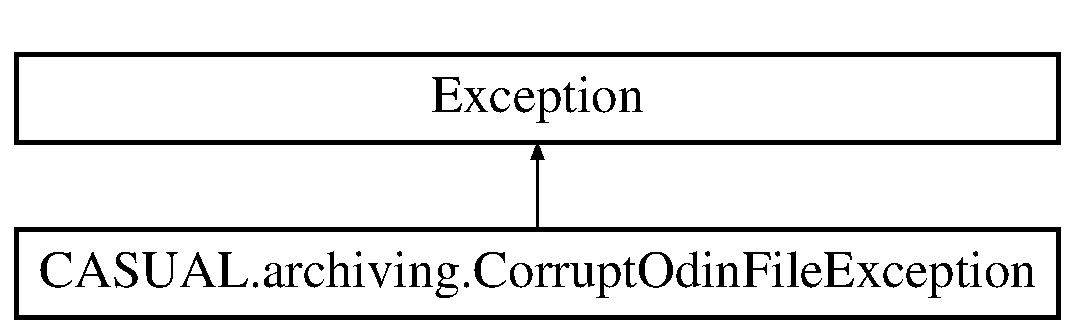
\includegraphics[height=2.000000cm]{classCASUAL_1_1archiving_1_1CorruptOdinFileException}
\end{center}
\end{figure}
\subsection*{Public Member Functions}
\begin{DoxyCompactItemize}
\item 
\hypertarget{classCASUAL_1_1archiving_1_1CorruptOdinFileException_af0eb2e388f2705ab50b2e8371eea1f53}{{\bfseries Corrupt\-Odin\-File\-Exception} (String error)}\label{classCASUAL_1_1archiving_1_1CorruptOdinFileException_af0eb2e388f2705ab50b2e8371eea1f53}

\end{DoxyCompactItemize}


\subsection{Detailed Description}
\begin{DoxyAuthor}{Author}
adamoutler 
\end{DoxyAuthor}


The documentation for this class was generated from the following file\-:\begin{DoxyCompactItemize}
\item 
trunk/\-C\-A\-S\-U\-A\-Lcore/src/\-C\-A\-S\-U\-A\-L/archiving/Corrupt\-Odin\-File\-Exception.\-java\end{DoxyCompactItemize}

\hypertarget{classCASUAL_1_1CountLines}{\section{C\-A\-S\-U\-A\-L.\-Count\-Lines Class Reference}
\label{classCASUAL_1_1CountLines}\index{C\-A\-S\-U\-A\-L.\-Count\-Lines@{C\-A\-S\-U\-A\-L.\-Count\-Lines}}
}
\subsection*{Public Member Functions}
\begin{DoxyCompactItemize}
\item 
\hypertarget{classCASUAL_1_1CountLines_a5bdad6b7a532e6447b8261abe908e1b4}{int {\bfseries count\-File\-Lines} (String Filename)}\label{classCASUAL_1_1CountLines_a5bdad6b7a532e6447b8261abe908e1b4}

\item 
\hypertarget{classCASUAL_1_1CountLines_a5e38da91ee4a1578b101ec722a06af94}{int {\bfseries count\-Resource\-Lines} (String Resource\-Name)}\label{classCASUAL_1_1CountLines_a5e38da91ee4a1578b101ec722a06af94}

\item 
\hypertarget{classCASUAL_1_1CountLines_a5bdad6b7a532e6447b8261abe908e1b4}{int {\bfseries count\-File\-Lines} (String Filename)}\label{classCASUAL_1_1CountLines_a5bdad6b7a532e6447b8261abe908e1b4}

\item 
\hypertarget{classCASUAL_1_1CountLines_a5e38da91ee4a1578b101ec722a06af94}{int {\bfseries count\-Resource\-Lines} (String Resource\-Name)}\label{classCASUAL_1_1CountLines_a5e38da91ee4a1578b101ec722a06af94}

\end{DoxyCompactItemize}


\subsection{Detailed Description}
\begin{DoxyAuthor}{Author}
adam 
\end{DoxyAuthor}


The documentation for this class was generated from the following files\-:\begin{DoxyCompactItemize}
\item 
branches/\-C\-A\-S\-U\-A\-L-\/\-Headless/\-G\-U\-I/src/\-C\-A\-S\-U\-A\-L/Count\-Lines.\-java\item 
branches/\-Testing\-Branch/\-G\-Doc/src/\-C\-A\-S\-U\-A\-L/Count\-Lines.\-java\end{DoxyCompactItemize}

\hypertarget{classCASUAL_1_1misc_1_1CountLines}{\section{C\-A\-S\-U\-A\-L.\-misc.\-Count\-Lines Class Reference}
\label{classCASUAL_1_1misc_1_1CountLines}\index{C\-A\-S\-U\-A\-L.\-misc.\-Count\-Lines@{C\-A\-S\-U\-A\-L.\-misc.\-Count\-Lines}}
}
\subsection*{Public Member Functions}
\begin{DoxyCompactItemize}
\item 
int \hyperlink{classCASUAL_1_1misc_1_1CountLines_a617b2984f9c9bd62dd346f2ea26ea07f}{count\-File\-Lines} (String Filename)
\item 
int \hyperlink{classCASUAL_1_1misc_1_1CountLines_a548bd64e69e6f19f8345de5f6dbf6e08}{count\-Resource\-Lines} (String Resource\-Name)
\item 
int \hyperlink{classCASUAL_1_1misc_1_1CountLines_a1e6760716b96cfa27677f6b8a4d66b69}{count\-I\-S\-Lines} (Input\-Stream I\-S)  throws I\-O\-Exception 
\end{DoxyCompactItemize}


\subsection{Detailed Description}
\begin{DoxyAuthor}{Author}
adam 
\end{DoxyAuthor}


\subsection{Member Function Documentation}
\hypertarget{classCASUAL_1_1misc_1_1CountLines_a617b2984f9c9bd62dd346f2ea26ea07f}{\index{C\-A\-S\-U\-A\-L\-::misc\-::\-Count\-Lines@{C\-A\-S\-U\-A\-L\-::misc\-::\-Count\-Lines}!count\-File\-Lines@{count\-File\-Lines}}
\index{count\-File\-Lines@{count\-File\-Lines}!CASUAL::misc::CountLines@{C\-A\-S\-U\-A\-L\-::misc\-::\-Count\-Lines}}
\subsubsection[{count\-File\-Lines}]{\setlength{\rightskip}{0pt plus 5cm}int C\-A\-S\-U\-A\-L.\-misc.\-Count\-Lines.\-count\-File\-Lines (
\begin{DoxyParamCaption}
\item[{String}]{Filename}
\end{DoxyParamCaption}
)}}\label{classCASUAL_1_1misc_1_1CountLines_a617b2984f9c9bd62dd346f2ea26ea07f}
Counts lines in a file


\begin{DoxyParams}{Parameters}
{\em Filename} & \\
\hline
\end{DoxyParams}
\begin{DoxyReturn}{Returns}
number of lines in a file 
\end{DoxyReturn}
\hypertarget{classCASUAL_1_1misc_1_1CountLines_a1e6760716b96cfa27677f6b8a4d66b69}{\index{C\-A\-S\-U\-A\-L\-::misc\-::\-Count\-Lines@{C\-A\-S\-U\-A\-L\-::misc\-::\-Count\-Lines}!count\-I\-S\-Lines@{count\-I\-S\-Lines}}
\index{count\-I\-S\-Lines@{count\-I\-S\-Lines}!CASUAL::misc::CountLines@{C\-A\-S\-U\-A\-L\-::misc\-::\-Count\-Lines}}
\subsubsection[{count\-I\-S\-Lines}]{\setlength{\rightskip}{0pt plus 5cm}int C\-A\-S\-U\-A\-L.\-misc.\-Count\-Lines.\-count\-I\-S\-Lines (
\begin{DoxyParamCaption}
\item[{Input\-Stream}]{I\-S}
\end{DoxyParamCaption}
) throws I\-O\-Exception}}\label{classCASUAL_1_1misc_1_1CountLines_a1e6760716b96cfa27677f6b8a4d66b69}
counts number of lines in an inputstream based on \char`\"{}\textbackslash{}n\char`\"{} character usage 
\begin{DoxyParams}{Parameters}
{\em I\-S} & inputstream to be checked \\
\hline
\end{DoxyParams}
\begin{DoxyReturn}{Returns}
number of lines counted in the stream 
\end{DoxyReturn}

\begin{DoxyExceptions}{Exceptions}
{\em I\-O\-Exception} & \\
\hline
\end{DoxyExceptions}
\hypertarget{classCASUAL_1_1misc_1_1CountLines_a548bd64e69e6f19f8345de5f6dbf6e08}{\index{C\-A\-S\-U\-A\-L\-::misc\-::\-Count\-Lines@{C\-A\-S\-U\-A\-L\-::misc\-::\-Count\-Lines}!count\-Resource\-Lines@{count\-Resource\-Lines}}
\index{count\-Resource\-Lines@{count\-Resource\-Lines}!CASUAL::misc::CountLines@{C\-A\-S\-U\-A\-L\-::misc\-::\-Count\-Lines}}
\subsubsection[{count\-Resource\-Lines}]{\setlength{\rightskip}{0pt plus 5cm}int C\-A\-S\-U\-A\-L.\-misc.\-Count\-Lines.\-count\-Resource\-Lines (
\begin{DoxyParamCaption}
\item[{String}]{Resource\-Name}
\end{DoxyParamCaption}
)}}\label{classCASUAL_1_1misc_1_1CountLines_a548bd64e69e6f19f8345de5f6dbf6e08}
Takes a resource and returns number of new lines.


\begin{DoxyParams}{Parameters}
{\em Resource\-Name} & \\
\hline
\end{DoxyParams}
\begin{DoxyReturn}{Returns}
number of lines in a file 
\end{DoxyReturn}


The documentation for this class was generated from the following file\-:\begin{DoxyCompactItemize}
\item 
trunk/\-C\-A\-S\-U\-A\-Lcore/src/\-C\-A\-S\-U\-A\-L/misc/Count\-Lines.\-java\end{DoxyCompactItemize}

\hypertarget{classdevicedetector_1_1DeviceDetector}{\section{devicedetector.\-Device\-Detector Class Reference}
\label{classdevicedetector_1_1DeviceDetector}\index{devicedetector.\-Device\-Detector@{devicedetector.\-Device\-Detector}}
}
\subsection*{Public Member Functions}
\begin{DoxyCompactItemize}
\item 
\hypertarget{classdevicedetector_1_1DeviceDetector_a22444bf7f452eef8f7b87613258ce518}{void {\bfseries run} (String\mbox{[}$\,$\mbox{]} args)}\label{classdevicedetector_1_1DeviceDetector_a22444bf7f452eef8f7b87613258ce518}

\end{DoxyCompactItemize}
\subsection*{Static Public Member Functions}
\begin{DoxyCompactItemize}
\item 
static void \hyperlink{classdevicedetector_1_1DeviceDetector_a8a2b4aee49c19024f1c0e85039bef361}{main} (String\mbox{[}$\,$\mbox{]} args)
\end{DoxyCompactItemize}


\subsection{Detailed Description}
\begin{DoxyAuthor}{Author}
loganludington 
\end{DoxyAuthor}


\subsection{Member Function Documentation}
\hypertarget{classdevicedetector_1_1DeviceDetector_a8a2b4aee49c19024f1c0e85039bef361}{\index{devicedetector\-::\-Device\-Detector@{devicedetector\-::\-Device\-Detector}!main@{main}}
\index{main@{main}!devicedetector::DeviceDetector@{devicedetector\-::\-Device\-Detector}}
\subsubsection[{main}]{\setlength{\rightskip}{0pt plus 5cm}static void devicedetector.\-Device\-Detector.\-main (
\begin{DoxyParamCaption}
\item[{String\mbox{[}$\,$\mbox{]}}]{args}
\end{DoxyParamCaption}
)\hspace{0.3cm}{\ttfamily [static]}}}\label{classdevicedetector_1_1DeviceDetector_a8a2b4aee49c19024f1c0e85039bef361}

\begin{DoxyParams}{Parameters}
{\em args} & the command line arguments \\
\hline
\end{DoxyParams}


The documentation for this class was generated from the following file\-:\begin{DoxyCompactItemize}
\item 
branches/\-Testing\-Branch/\-Device\-Detector/src/devicedetector/Device\-Detector.\-java\end{DoxyCompactItemize}

\hypertarget{classCASUAL_1_1DiffTextFiles}{\section{C\-A\-S\-U\-A\-L.\-Diff\-Text\-Files Class Reference}
\label{classCASUAL_1_1DiffTextFiles}\index{C\-A\-S\-U\-A\-L.\-Diff\-Text\-Files@{C\-A\-S\-U\-A\-L.\-Diff\-Text\-Files}}
}
\subsection*{Public Member Functions}
\begin{DoxyCompactItemize}
\item 
\hypertarget{classCASUAL_1_1DiffTextFiles_a0e4688f916157ad380172b563f289882}{String {\bfseries diff\-Resource\-Versus\-File} (String Test\-I\-Stream, String Original\-File)}\label{classCASUAL_1_1DiffTextFiles_a0e4688f916157ad380172b563f289882}

\item 
\hypertarget{classCASUAL_1_1DiffTextFiles_a15391ab2129d297765c49700e5e174a8}{String {\bfseries diff\-Text\-Files} (String Original, String Test\-For\-Diff)}\label{classCASUAL_1_1DiffTextFiles_a15391ab2129d297765c49700e5e174a8}

\item 
\hypertarget{classCASUAL_1_1DiffTextFiles_a2781947d0eddb10d4536698a56f08112}{void {\bfseries append\-Diff\-To\-File} (String Name\-Of\-File\-To\-Be\-Modified, String Diff)}\label{classCASUAL_1_1DiffTextFiles_a2781947d0eddb10d4536698a56f08112}

\item 
\hypertarget{classCASUAL_1_1DiffTextFiles_a0e4688f916157ad380172b563f289882}{String {\bfseries diff\-Resource\-Versus\-File} (String Test\-I\-Stream, String Original\-File)}\label{classCASUAL_1_1DiffTextFiles_a0e4688f916157ad380172b563f289882}

\item 
\hypertarget{classCASUAL_1_1DiffTextFiles_a15391ab2129d297765c49700e5e174a8}{String {\bfseries diff\-Text\-Files} (String Original, String Test\-For\-Diff)}\label{classCASUAL_1_1DiffTextFiles_a15391ab2129d297765c49700e5e174a8}

\item 
\hypertarget{classCASUAL_1_1DiffTextFiles_a2781947d0eddb10d4536698a56f08112}{void {\bfseries append\-Diff\-To\-File} (String Name\-Of\-File\-To\-Be\-Modified, String Diff)}\label{classCASUAL_1_1DiffTextFiles_a2781947d0eddb10d4536698a56f08112}

\end{DoxyCompactItemize}


\subsection{Detailed Description}
\begin{DoxyAuthor}{Author}
Logans\-A\-L\-I\-E\-N 
\end{DoxyAuthor}


The documentation for this class was generated from the following files\-:\begin{DoxyCompactItemize}
\item 
branches/\-C\-A\-S\-U\-A\-L-\/\-Headless/\-G\-U\-I/src/\-C\-A\-S\-U\-A\-L/Diff\-Text\-Files.\-java\item 
branches/\-Testing\-Branch/\-G\-Doc/src/\-C\-A\-S\-U\-A\-L/Diff\-Text\-Files.\-java\end{DoxyCompactItemize}

\hypertarget{classCASUAL_1_1misc_1_1DiffTextFiles}{\section{C\-A\-S\-U\-A\-L.\-misc.\-Diff\-Text\-Files Class Reference}
\label{classCASUAL_1_1misc_1_1DiffTextFiles}\index{C\-A\-S\-U\-A\-L.\-misc.\-Diff\-Text\-Files@{C\-A\-S\-U\-A\-L.\-misc.\-Diff\-Text\-Files}}
}
\subsection*{Public Member Functions}
\begin{DoxyCompactItemize}
\item 
String \hyperlink{classCASUAL_1_1misc_1_1DiffTextFiles_a7eb69fa4b7c445f249e91417d8d5b650}{diff\-Resource\-Versus\-File} (String Test\-I\-Stream, String Original\-File)
\item 
String \hyperlink{classCASUAL_1_1misc_1_1DiffTextFiles_ad17653963cb2e8309c0b04139da4174b}{diff\-Text\-Files} (String Original, String Test\-For\-Diff)
\item 
void \hyperlink{classCASUAL_1_1misc_1_1DiffTextFiles_af859cc974cfa051c3e0f6b78c1d875ff}{append\-Diff\-To\-File} (String Name\-Of\-File\-To\-Be\-Modified, String Diff)
\end{DoxyCompactItemize}


\subsection{Detailed Description}
\begin{DoxyAuthor}{Author}
Logans\-A\-L\-I\-E\-N 
\end{DoxyAuthor}


\subsection{Member Function Documentation}
\hypertarget{classCASUAL_1_1misc_1_1DiffTextFiles_af859cc974cfa051c3e0f6b78c1d875ff}{\index{C\-A\-S\-U\-A\-L\-::misc\-::\-Diff\-Text\-Files@{C\-A\-S\-U\-A\-L\-::misc\-::\-Diff\-Text\-Files}!append\-Diff\-To\-File@{append\-Diff\-To\-File}}
\index{append\-Diff\-To\-File@{append\-Diff\-To\-File}!CASUAL::misc::DiffTextFiles@{C\-A\-S\-U\-A\-L\-::misc\-::\-Diff\-Text\-Files}}
\subsubsection[{append\-Diff\-To\-File}]{\setlength{\rightskip}{0pt plus 5cm}void C\-A\-S\-U\-A\-L.\-misc.\-Diff\-Text\-Files.\-append\-Diff\-To\-File (
\begin{DoxyParamCaption}
\item[{String}]{Name\-Of\-File\-To\-Be\-Modified, }
\item[{String}]{Diff}
\end{DoxyParamCaption}
)}}\label{classCASUAL_1_1misc_1_1DiffTextFiles_af859cc974cfa051c3e0f6b78c1d875ff}
appends text to file


\begin{DoxyParams}{Parameters}
{\em Name\-Of\-File\-To\-Be\-Modified} & file to be appended \\
\hline
{\em Diff} & text to add \\
\hline
\end{DoxyParams}
\hypertarget{classCASUAL_1_1misc_1_1DiffTextFiles_a7eb69fa4b7c445f249e91417d8d5b650}{\index{C\-A\-S\-U\-A\-L\-::misc\-::\-Diff\-Text\-Files@{C\-A\-S\-U\-A\-L\-::misc\-::\-Diff\-Text\-Files}!diff\-Resource\-Versus\-File@{diff\-Resource\-Versus\-File}}
\index{diff\-Resource\-Versus\-File@{diff\-Resource\-Versus\-File}!CASUAL::misc::DiffTextFiles@{C\-A\-S\-U\-A\-L\-::misc\-::\-Diff\-Text\-Files}}
\subsubsection[{diff\-Resource\-Versus\-File}]{\setlength{\rightskip}{0pt plus 5cm}String C\-A\-S\-U\-A\-L.\-misc.\-Diff\-Text\-Files.\-diff\-Resource\-Versus\-File (
\begin{DoxyParamCaption}
\item[{String}]{Test\-I\-Stream, }
\item[{String}]{Original\-File}
\end{DoxyParamCaption}
)}}\label{classCASUAL_1_1misc_1_1DiffTextFiles_a7eb69fa4b7c445f249e91417d8d5b650}
takes a resource and a string outputs difference as a string


\begin{DoxyParams}{Parameters}
{\em Test\-I\-Stream} & input stream to test \\
\hline
{\em Original\-File} & original file to be diffed \\
\hline
\end{DoxyParams}
\begin{DoxyReturn}{Returns}
lines in test that are not in original 
\end{DoxyReturn}
\hypertarget{classCASUAL_1_1misc_1_1DiffTextFiles_ad17653963cb2e8309c0b04139da4174b}{\index{C\-A\-S\-U\-A\-L\-::misc\-::\-Diff\-Text\-Files@{C\-A\-S\-U\-A\-L\-::misc\-::\-Diff\-Text\-Files}!diff\-Text\-Files@{diff\-Text\-Files}}
\index{diff\-Text\-Files@{diff\-Text\-Files}!CASUAL::misc::DiffTextFiles@{C\-A\-S\-U\-A\-L\-::misc\-::\-Diff\-Text\-Files}}
\subsubsection[{diff\-Text\-Files}]{\setlength{\rightskip}{0pt plus 5cm}String C\-A\-S\-U\-A\-L.\-misc.\-Diff\-Text\-Files.\-diff\-Text\-Files (
\begin{DoxyParamCaption}
\item[{String}]{Original, }
\item[{String}]{Test\-For\-Diff}
\end{DoxyParamCaption}
)}}\label{classCASUAL_1_1misc_1_1DiffTextFiles_ad17653963cb2e8309c0b04139da4174b}
takes two files returns the difference between the two


\begin{DoxyParams}{Parameters}
{\em Original} & original file \\
\hline
{\em Test\-For\-Diff} & new file \\
\hline
\end{DoxyParams}
\begin{DoxyReturn}{Returns}
lines which are in new file that are not in original 
\end{DoxyReturn}


The documentation for this class was generated from the following file\-:\begin{DoxyCompactItemize}
\item 
trunk/\-C\-A\-S\-U\-A\-Lcore/src/\-C\-A\-S\-U\-A\-L/misc/Diff\-Text\-Files.\-java\end{DoxyCompactItemize}

\hypertarget{classCASUAL_1_1gDrive_1_1downUpProgress}{\section{C\-A\-S\-U\-A\-L.\-g\-Drive.\-down\-Up\-Progress Class Reference}
\label{classCASUAL_1_1gDrive_1_1downUpProgress}\index{C\-A\-S\-U\-A\-L.\-g\-Drive.\-down\-Up\-Progress@{C\-A\-S\-U\-A\-L.\-g\-Drive.\-down\-Up\-Progress}}
}
Inheritance diagram for C\-A\-S\-U\-A\-L.\-g\-Drive.\-down\-Up\-Progress\-:\begin{figure}[H]
\begin{center}
\leavevmode
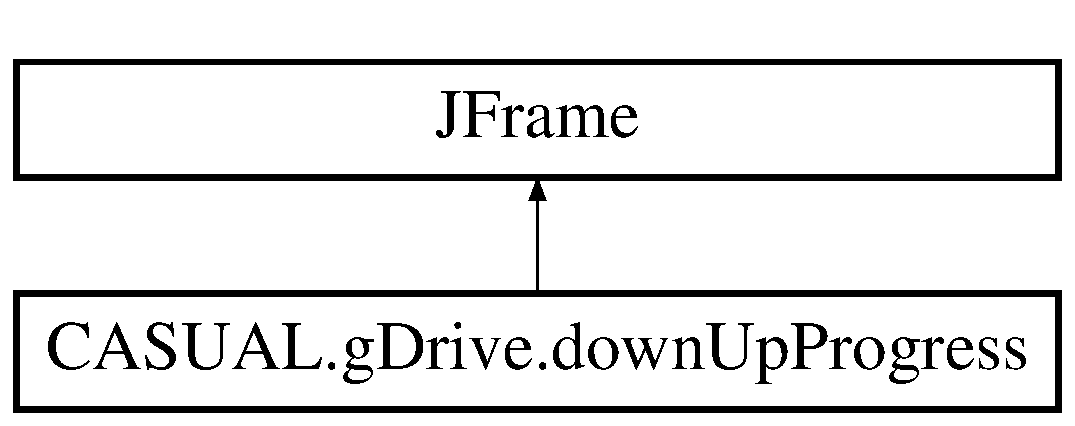
\includegraphics[height=2.000000cm]{classCASUAL_1_1gDrive_1_1downUpProgress}
\end{center}
\end{figure}
\subsection*{Public Member Functions}
\begin{DoxyCompactItemize}
\item 
\hyperlink{classCASUAL_1_1gDrive_1_1downUpProgress_aace68e5af54d1bb957854705bd3aa9ed}{down\-Up\-Progress} (String name, boolean download)
\item 
\hypertarget{classCASUAL_1_1gDrive_1_1downUpProgress_a6a453b0639457ecd9a777a10b8f8f31c}{void {\bfseries update\-Progress} (int progress)}\label{classCASUAL_1_1gDrive_1_1downUpProgress_a6a453b0639457ecd9a777a10b8f8f31c}

\end{DoxyCompactItemize}
\subsection*{Static Public Member Functions}
\begin{DoxyCompactItemize}
\item 
static void \hyperlink{classCASUAL_1_1gDrive_1_1downUpProgress_a9c4dd83cfc683cf0575776ebf14dcaf7}{main} (String args\mbox{[}$\,$\mbox{]})
\end{DoxyCompactItemize}


\subsection{Detailed Description}
\begin{DoxyAuthor}{Author}
loglud 
\end{DoxyAuthor}


\subsection{Constructor \& Destructor Documentation}
\hypertarget{classCASUAL_1_1gDrive_1_1downUpProgress_aace68e5af54d1bb957854705bd3aa9ed}{\index{C\-A\-S\-U\-A\-L\-::g\-Drive\-::down\-Up\-Progress@{C\-A\-S\-U\-A\-L\-::g\-Drive\-::down\-Up\-Progress}!down\-Up\-Progress@{down\-Up\-Progress}}
\index{down\-Up\-Progress@{down\-Up\-Progress}!CASUAL::gDrive::downUpProgress@{C\-A\-S\-U\-A\-L\-::g\-Drive\-::down\-Up\-Progress}}
\subsubsection[{down\-Up\-Progress}]{\setlength{\rightskip}{0pt plus 5cm}C\-A\-S\-U\-A\-L.\-g\-Drive.\-down\-Up\-Progress.\-down\-Up\-Progress (
\begin{DoxyParamCaption}
\item[{String}]{name, }
\item[{boolean}]{download}
\end{DoxyParamCaption}
)}}\label{classCASUAL_1_1gDrive_1_1downUpProgress_aace68e5af54d1bb957854705bd3aa9ed}
Creates new form \hyperlink{classCASUAL_1_1gDrive_1_1downUpProgress}{down\-Up\-Progress} 

\subsection{Member Function Documentation}
\hypertarget{classCASUAL_1_1gDrive_1_1downUpProgress_a9c4dd83cfc683cf0575776ebf14dcaf7}{\index{C\-A\-S\-U\-A\-L\-::g\-Drive\-::down\-Up\-Progress@{C\-A\-S\-U\-A\-L\-::g\-Drive\-::down\-Up\-Progress}!main@{main}}
\index{main@{main}!CASUAL::gDrive::downUpProgress@{C\-A\-S\-U\-A\-L\-::g\-Drive\-::down\-Up\-Progress}}
\subsubsection[{main}]{\setlength{\rightskip}{0pt plus 5cm}static void C\-A\-S\-U\-A\-L.\-g\-Drive.\-down\-Up\-Progress.\-main (
\begin{DoxyParamCaption}
\item[{String}]{args\mbox{[}$\,$\mbox{]}}
\end{DoxyParamCaption}
)\hspace{0.3cm}{\ttfamily [static]}}}\label{classCASUAL_1_1gDrive_1_1downUpProgress_a9c4dd83cfc683cf0575776ebf14dcaf7}

\begin{DoxyParams}{Parameters}
{\em args} & the command line arguments \\
\hline
\end{DoxyParams}


The documentation for this class was generated from the following file\-:\begin{DoxyCompactItemize}
\item 
branches/\-Testing\-Branch/\-G\-Doc/src/\-C\-A\-S\-U\-A\-L/g\-Drive/down\-Up\-Progress.\-java\end{DoxyCompactItemize}

\hypertarget{classCASUAL_1_1FastbootTools}{\section{C\-A\-S\-U\-A\-L.\-Fastboot\-Tools Class Reference}
\label{classCASUAL_1_1FastbootTools}\index{C\-A\-S\-U\-A\-L.\-Fastboot\-Tools@{C\-A\-S\-U\-A\-L.\-Fastboot\-Tools}}
}
\subsection*{Public Member Functions}
\begin{DoxyCompactItemize}
\item 
String \hyperlink{classCASUAL_1_1FastbootTools_a987c870343c7a351e86be883e6b5ba65}{do\-Fastboot\-Shell\-Command} (String line)
\item 
String \hyperlink{classCASUAL_1_1FastbootTools_a2d7a1dc5dcdefce4b15844be2736dff5}{do\-Elevated\-Fastboot\-Shell\-Command} (String line)
\end{DoxyCompactItemize}
\subsection*{Static Public Member Functions}
\begin{DoxyCompactItemize}
\item 
static void \hyperlink{classCASUAL_1_1FastbootTools_a480cf5e63970928c8d7e2d881250c58c}{check\-And\-Deploy\-Fastboot} ()
\item 
static String \hyperlink{classCASUAL_1_1FastbootTools_a20125879a0b7d54b8f43c75fc74108ae}{get\-Fastboot\-Linux\-Resource} ()
\end{DoxyCompactItemize}


\subsection{Detailed Description}
\begin{DoxyAuthor}{Author}
adam 
\end{DoxyAuthor}


\subsection{Member Function Documentation}
\hypertarget{classCASUAL_1_1FastbootTools_a480cf5e63970928c8d7e2d881250c58c}{\index{C\-A\-S\-U\-A\-L\-::\-Fastboot\-Tools@{C\-A\-S\-U\-A\-L\-::\-Fastboot\-Tools}!check\-And\-Deploy\-Fastboot@{check\-And\-Deploy\-Fastboot}}
\index{check\-And\-Deploy\-Fastboot@{check\-And\-Deploy\-Fastboot}!CASUAL::FastbootTools@{C\-A\-S\-U\-A\-L\-::\-Fastboot\-Tools}}
\subsubsection[{check\-And\-Deploy\-Fastboot}]{\setlength{\rightskip}{0pt plus 5cm}static void C\-A\-S\-U\-A\-L.\-Fastboot\-Tools.\-check\-And\-Deploy\-Fastboot (
\begin{DoxyParamCaption}
{}
\end{DoxyParamCaption}
)\hspace{0.3cm}{\ttfamily [static]}}}\label{classCASUAL_1_1FastbootTools_a480cf5e63970928c8d7e2d881250c58c}
deploys and verifies fastboot \hypertarget{classCASUAL_1_1FastbootTools_a2d7a1dc5dcdefce4b15844be2736dff5}{\index{C\-A\-S\-U\-A\-L\-::\-Fastboot\-Tools@{C\-A\-S\-U\-A\-L\-::\-Fastboot\-Tools}!do\-Elevated\-Fastboot\-Shell\-Command@{do\-Elevated\-Fastboot\-Shell\-Command}}
\index{do\-Elevated\-Fastboot\-Shell\-Command@{do\-Elevated\-Fastboot\-Shell\-Command}!CASUAL::FastbootTools@{C\-A\-S\-U\-A\-L\-::\-Fastboot\-Tools}}
\subsubsection[{do\-Elevated\-Fastboot\-Shell\-Command}]{\setlength{\rightskip}{0pt plus 5cm}String C\-A\-S\-U\-A\-L.\-Fastboot\-Tools.\-do\-Elevated\-Fastboot\-Shell\-Command (
\begin{DoxyParamCaption}
\item[{String}]{line}
\end{DoxyParamCaption}
)}}\label{classCASUAL_1_1FastbootTools_a2d7a1dc5dcdefce4b15844be2736dff5}
performs elevated fastboot command


\begin{DoxyParams}{Parameters}
{\em line} & params for fastboot \\
\hline
\end{DoxyParams}
\begin{DoxyReturn}{Returns}
value from fastboot command 
\end{DoxyReturn}
\hypertarget{classCASUAL_1_1FastbootTools_a987c870343c7a351e86be883e6b5ba65}{\index{C\-A\-S\-U\-A\-L\-::\-Fastboot\-Tools@{C\-A\-S\-U\-A\-L\-::\-Fastboot\-Tools}!do\-Fastboot\-Shell\-Command@{do\-Fastboot\-Shell\-Command}}
\index{do\-Fastboot\-Shell\-Command@{do\-Fastboot\-Shell\-Command}!CASUAL::FastbootTools@{C\-A\-S\-U\-A\-L\-::\-Fastboot\-Tools}}
\subsubsection[{do\-Fastboot\-Shell\-Command}]{\setlength{\rightskip}{0pt plus 5cm}String C\-A\-S\-U\-A\-L.\-Fastboot\-Tools.\-do\-Fastboot\-Shell\-Command (
\begin{DoxyParamCaption}
\item[{String}]{line}
\end{DoxyParamCaption}
)}}\label{classCASUAL_1_1FastbootTools_a987c870343c7a351e86be883e6b5ba65}
executes fastboot


\begin{DoxyParams}{Parameters}
{\em line} & params for fastboot \\
\hline
\end{DoxyParams}
\begin{DoxyReturn}{Returns}
value from fastboot command 
\end{DoxyReturn}
\hypertarget{classCASUAL_1_1FastbootTools_a20125879a0b7d54b8f43c75fc74108ae}{\index{C\-A\-S\-U\-A\-L\-::\-Fastboot\-Tools@{C\-A\-S\-U\-A\-L\-::\-Fastboot\-Tools}!get\-Fastboot\-Linux\-Resource@{get\-Fastboot\-Linux\-Resource}}
\index{get\-Fastboot\-Linux\-Resource@{get\-Fastboot\-Linux\-Resource}!CASUAL::FastbootTools@{C\-A\-S\-U\-A\-L\-::\-Fastboot\-Tools}}
\subsubsection[{get\-Fastboot\-Linux\-Resource}]{\setlength{\rightskip}{0pt plus 5cm}static String C\-A\-S\-U\-A\-L.\-Fastboot\-Tools.\-get\-Fastboot\-Linux\-Resource (
\begin{DoxyParamCaption}
{}
\end{DoxyParamCaption}
)\hspace{0.3cm}{\ttfamily [static]}}}\label{classCASUAL_1_1FastbootTools_a20125879a0b7d54b8f43c75fc74108ae}
gets the resource for Fastboot

\begin{DoxyReturn}{Returns}
path to resource 
\end{DoxyReturn}


The documentation for this class was generated from the following file\-:\begin{DoxyCompactItemize}
\item 
trunk/\-C\-A\-S\-U\-A\-Lcore/src/\-C\-A\-S\-U\-A\-L/Fastboot\-Tools.\-java\end{DoxyCompactItemize}

\hypertarget{classCASUAL_1_1gDrive_1_1FileDownloadProgressListener}{\section{C\-A\-S\-U\-A\-L.\-g\-Drive.\-File\-Download\-Progress\-Listener Class Reference}
\label{classCASUAL_1_1gDrive_1_1FileDownloadProgressListener}\index{C\-A\-S\-U\-A\-L.\-g\-Drive.\-File\-Download\-Progress\-Listener@{C\-A\-S\-U\-A\-L.\-g\-Drive.\-File\-Download\-Progress\-Listener}}
}
Inheritance diagram for C\-A\-S\-U\-A\-L.\-g\-Drive.\-File\-Download\-Progress\-Listener\-:\begin{figure}[H]
\begin{center}
\leavevmode
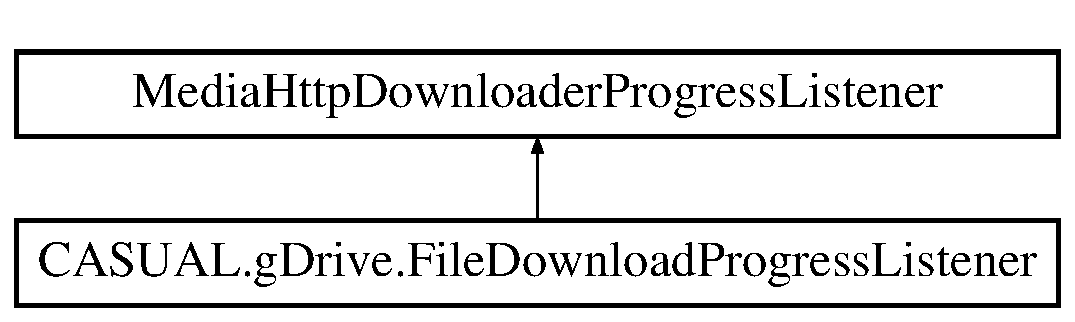
\includegraphics[height=2.000000cm]{classCASUAL_1_1gDrive_1_1FileDownloadProgressListener}
\end{center}
\end{figure}
\subsection*{Public Member Functions}
\begin{DoxyCompactItemize}
\item 
\hypertarget{classCASUAL_1_1gDrive_1_1FileDownloadProgressListener_a7e6a8545cee584856f2875eb1ab32f12}{{\bfseries File\-Download\-Progress\-Listener} (String name)}\label{classCASUAL_1_1gDrive_1_1FileDownloadProgressListener_a7e6a8545cee584856f2875eb1ab32f12}

\item 
\hypertarget{classCASUAL_1_1gDrive_1_1FileDownloadProgressListener_ad70b34a02a48d49c178d45b2885e8c20}{void {\bfseries progress\-Changed} (Media\-Http\-Downloader downloader)}\label{classCASUAL_1_1gDrive_1_1FileDownloadProgressListener_ad70b34a02a48d49c178d45b2885e8c20}

\end{DoxyCompactItemize}
\subsection*{Public Attributes}
\begin{DoxyCompactItemize}
\item 
\hypertarget{classCASUAL_1_1gDrive_1_1FileDownloadProgressListener_af6c4febdd75950f128f3065d81abcff2}{\hyperlink{classCASUAL_1_1gDrive_1_1downUpProgress}{down\-Up\-Progress} {\bfseries dlp}}\label{classCASUAL_1_1gDrive_1_1FileDownloadProgressListener_af6c4febdd75950f128f3065d81abcff2}

\end{DoxyCompactItemize}


\subsection{Detailed Description}
\begin{DoxyAuthor}{Author}
loglud 
\end{DoxyAuthor}


The documentation for this class was generated from the following file\-:\begin{DoxyCompactItemize}
\item 
branches/\-Testing\-Branch/\-G\-Doc/src/\-C\-A\-S\-U\-A\-L/g\-Drive/File\-Download\-Progress\-Listener.\-java\end{DoxyCompactItemize}

\hypertarget{classCASUAL_1_1FileOperations}{\section{C\-A\-S\-U\-A\-L.\-File\-Operations Class Reference}
\label{classCASUAL_1_1FileOperations}\index{C\-A\-S\-U\-A\-L.\-File\-Operations@{C\-A\-S\-U\-A\-L.\-File\-Operations}}
}
\subsection*{Public Member Functions}
\begin{DoxyCompactItemize}
\item 
\hypertarget{classCASUAL_1_1FileOperations_a4e114f0c6001493ca5ed892e59276420}{boolean {\bfseries copy\-From\-Resource\-To\-File} (String Resource, String to\-File)}\label{classCASUAL_1_1FileOperations_a4e114f0c6001493ca5ed892e59276420}

\item 
\hypertarget{classCASUAL_1_1FileOperations_a8bf6613169e83dee9b70179e1331d99d}{void {\bfseries recursive\-Delete} (String path)}\label{classCASUAL_1_1FileOperations_a8bf6613169e83dee9b70179e1331d99d}

\item 
\hypertarget{classCASUAL_1_1FileOperations_a5fed83c75685ff9516eab0c37658070d}{void {\bfseries recursive\-Delete} (File path)}\label{classCASUAL_1_1FileOperations_a5fed83c75685ff9516eab0c37658070d}

\item 
\hypertarget{classCASUAL_1_1FileOperations_ae522f99e553aaa391e65a8c54ae60083}{boolean {\bfseries verify\-Permissions\-Recursive} (String path)}\label{classCASUAL_1_1FileOperations_ae522f99e553aaa391e65a8c54ae60083}

\item 
\hypertarget{classCASUAL_1_1FileOperations_afe29c51ef53af5e44cc4aa61a9a103d0}{String {\bfseries find\-Recursive} (String Path\-To\-Search, String File\-Name)}\label{classCASUAL_1_1FileOperations_afe29c51ef53af5e44cc4aa61a9a103d0}

\item 
\hypertarget{classCASUAL_1_1FileOperations_a2f6eced2a42e01ee23478f3a0448b139}{boolean {\bfseries make\-Folder} (String Folder)}\label{classCASUAL_1_1FileOperations_a2f6eced2a42e01ee23478f3a0448b139}

\item 
\hypertarget{classCASUAL_1_1FileOperations_a5b1172ca44af911f74d127cd05bf1f72}{Boolean {\bfseries delete\-File} (String File\-Name)}\label{classCASUAL_1_1FileOperations_a5b1172ca44af911f74d127cd05bf1f72}

\item 
\hypertarget{classCASUAL_1_1FileOperations_a95b6013a6610a12798b5a245a741196a}{void {\bfseries copy\-File} (File source\-File, File dest\-File)  throws I\-O\-Exception }\label{classCASUAL_1_1FileOperations_a95b6013a6610a12798b5a245a741196a}

\item 
\hypertarget{classCASUAL_1_1FileOperations_a6218a9a8ce1c18711d59b844417adc8a}{String {\bfseries current\-Dir} ()}\label{classCASUAL_1_1FileOperations_a6218a9a8ce1c18711d59b844417adc8a}

\item 
\hypertarget{classCASUAL_1_1FileOperations_a13967d313b6bd64f4449872f39cd9850}{boolean {\bfseries copy\-File} (String From\-File, String To\-File)}\label{classCASUAL_1_1FileOperations_a13967d313b6bd64f4449872f39cd9850}

\item 
\hypertarget{classCASUAL_1_1FileOperations_a4c17ab8b3acd4d14bebfce16072ee88b}{boolean {\bfseries verify\-File\-Exists} (String Folder)}\label{classCASUAL_1_1FileOperations_a4c17ab8b3acd4d14bebfce16072ee88b}

\item 
\hypertarget{classCASUAL_1_1FileOperations_ad065441f27945626464c5ea2a5b1e453}{boolean {\bfseries set\-Executable\-Bit} (String Executable)}\label{classCASUAL_1_1FileOperations_ad065441f27945626464c5ea2a5b1e453}

\item 
\hypertarget{classCASUAL_1_1FileOperations_aeeab03412b9e7ae3ee245798e1e1b3d8}{boolean {\bfseries verify\-Resource} (String Res)}\label{classCASUAL_1_1FileOperations_aeeab03412b9e7ae3ee245798e1e1b3d8}

\item 
\hypertarget{classCASUAL_1_1FileOperations_af56078757baad2c1f1ce56bbe88ed583}{String {\bfseries read\-Text\-From\-Resource} (String Resource)}\label{classCASUAL_1_1FileOperations_af56078757baad2c1f1ce56bbe88ed583}

\item 
\hypertarget{classCASUAL_1_1FileOperations_a71fbad8531341fe6c2c5212aac13349d}{void {\bfseries write\-To\-File} (String Text, String File)  throws I\-O\-Exception}\label{classCASUAL_1_1FileOperations_a71fbad8531341fe6c2c5212aac13349d}

\item 
\hypertarget{classCASUAL_1_1FileOperations_a4e114f0c6001493ca5ed892e59276420}{boolean {\bfseries copy\-From\-Resource\-To\-File} (String Resource, String to\-File)}\label{classCASUAL_1_1FileOperations_a4e114f0c6001493ca5ed892e59276420}

\item 
\hypertarget{classCASUAL_1_1FileOperations_a8bf6613169e83dee9b70179e1331d99d}{void {\bfseries recursive\-Delete} (String path)}\label{classCASUAL_1_1FileOperations_a8bf6613169e83dee9b70179e1331d99d}

\item 
\hypertarget{classCASUAL_1_1FileOperations_a5fed83c75685ff9516eab0c37658070d}{void {\bfseries recursive\-Delete} (File path)}\label{classCASUAL_1_1FileOperations_a5fed83c75685ff9516eab0c37658070d}

\item 
\hypertarget{classCASUAL_1_1FileOperations_ae522f99e553aaa391e65a8c54ae60083}{boolean {\bfseries verify\-Permissions\-Recursive} (String path)}\label{classCASUAL_1_1FileOperations_ae522f99e553aaa391e65a8c54ae60083}

\item 
\hypertarget{classCASUAL_1_1FileOperations_afe29c51ef53af5e44cc4aa61a9a103d0}{String {\bfseries find\-Recursive} (String Path\-To\-Search, String File\-Name)}\label{classCASUAL_1_1FileOperations_afe29c51ef53af5e44cc4aa61a9a103d0}

\item 
\hypertarget{classCASUAL_1_1FileOperations_a2f6eced2a42e01ee23478f3a0448b139}{boolean {\bfseries make\-Folder} (String Folder)}\label{classCASUAL_1_1FileOperations_a2f6eced2a42e01ee23478f3a0448b139}

\item 
\hypertarget{classCASUAL_1_1FileOperations_a5b1172ca44af911f74d127cd05bf1f72}{Boolean {\bfseries delete\-File} (String File\-Name)}\label{classCASUAL_1_1FileOperations_a5b1172ca44af911f74d127cd05bf1f72}

\item 
\hypertarget{classCASUAL_1_1FileOperations_a95b6013a6610a12798b5a245a741196a}{void {\bfseries copy\-File} (File source\-File, File dest\-File)  throws I\-O\-Exception }\label{classCASUAL_1_1FileOperations_a95b6013a6610a12798b5a245a741196a}

\item 
\hypertarget{classCASUAL_1_1FileOperations_a6218a9a8ce1c18711d59b844417adc8a}{String {\bfseries current\-Dir} ()}\label{classCASUAL_1_1FileOperations_a6218a9a8ce1c18711d59b844417adc8a}

\item 
\hypertarget{classCASUAL_1_1FileOperations_a13967d313b6bd64f4449872f39cd9850}{boolean {\bfseries copy\-File} (String From\-File, String To\-File)}\label{classCASUAL_1_1FileOperations_a13967d313b6bd64f4449872f39cd9850}

\item 
\hypertarget{classCASUAL_1_1FileOperations_a4c17ab8b3acd4d14bebfce16072ee88b}{boolean {\bfseries verify\-File\-Exists} (String Folder)}\label{classCASUAL_1_1FileOperations_a4c17ab8b3acd4d14bebfce16072ee88b}

\item 
\hypertarget{classCASUAL_1_1FileOperations_ad065441f27945626464c5ea2a5b1e453}{boolean {\bfseries set\-Executable\-Bit} (String Executable)}\label{classCASUAL_1_1FileOperations_ad065441f27945626464c5ea2a5b1e453}

\item 
\hypertarget{classCASUAL_1_1FileOperations_aeeab03412b9e7ae3ee245798e1e1b3d8}{boolean {\bfseries verify\-Resource} (String Res)}\label{classCASUAL_1_1FileOperations_aeeab03412b9e7ae3ee245798e1e1b3d8}

\item 
\hypertarget{classCASUAL_1_1FileOperations_af56078757baad2c1f1ce56bbe88ed583}{String {\bfseries read\-Text\-From\-Resource} (String Resource)}\label{classCASUAL_1_1FileOperations_af56078757baad2c1f1ce56bbe88ed583}

\item 
\hypertarget{classCASUAL_1_1FileOperations_a71fbad8531341fe6c2c5212aac13349d}{void {\bfseries write\-To\-File} (String Text, String File)  throws I\-O\-Exception}\label{classCASUAL_1_1FileOperations_a71fbad8531341fe6c2c5212aac13349d}

\item 
\hyperlink{classCASUAL_1_1FileOperations_aee926f79c6ce0e347940b7a6114ab195}{File\-Operations} ()
\item 
boolean \hyperlink{classCASUAL_1_1FileOperations_a4e114f0c6001493ca5ed892e59276420}{copy\-From\-Resource\-To\-File} (String Resource, String to\-File)
\item 
void \hyperlink{classCASUAL_1_1FileOperations_a8bf6613169e83dee9b70179e1331d99d}{recursive\-Delete} (String path)
\item 
void \hyperlink{classCASUAL_1_1FileOperations_a5fed83c75685ff9516eab0c37658070d}{recursive\-Delete} (File path)
\item 
boolean \hyperlink{classCASUAL_1_1FileOperations_a222a88ab031762c4cc9197c3b6732baa}{verify\-Write\-Permissions\-Recursive} (String path)
\item 
String \hyperlink{classCASUAL_1_1FileOperations_afe29c51ef53af5e44cc4aa61a9a103d0}{find\-Recursive} (String Path\-To\-Search, String File\-Name)
\item 
boolean \hyperlink{classCASUAL_1_1FileOperations_ab8c755446ba87c4ef056cc2b156ee726}{verify\-Exists} (String file)
\item 
boolean \hyperlink{classCASUAL_1_1FileOperations_a2f6eced2a42e01ee23478f3a0448b139}{make\-Folder} (String Folder)
\item 
void \hyperlink{classCASUAL_1_1FileOperations_a76f17b62e1bbc87e3d557643c52e6672}{write\-Stream\-To\-File} (Buffered\-Input\-Stream stream, String destination)  throws File\-Not\-Found\-Exception, I\-O\-Exception 
\item 
void \hyperlink{classCASUAL_1_1FileOperations_a71fbad8531341fe6c2c5212aac13349d}{write\-To\-File} (String Text, String File)  throws I\-O\-Exception 
\item 
void \hyperlink{classCASUAL_1_1FileOperations_a6f67c5c95ce23d0d4163b56eddb8e28f}{overwrite\-File} (String Text, String File)  throws I\-O\-Exception 
\item 
Boolean \hyperlink{classCASUAL_1_1FileOperations_a5b1172ca44af911f74d127cd05bf1f72}{delete\-File} (String File\-Name)
\item 
boolean \hyperlink{classCASUAL_1_1FileOperations_a8e86ea11b79fef56147aba90dc3f4f0f}{delete\-String\-Array\-Of\-Files} (String\mbox{[}$\,$\mbox{]} clean\-Up)
\item 
void \hyperlink{classCASUAL_1_1FileOperations_a95b6013a6610a12798b5a245a741196a}{copy\-File} (File source\-File, File dest\-File)  throws I\-O\-Exception 
\item 
String \hyperlink{classCASUAL_1_1FileOperations_a6218a9a8ce1c18711d59b844417adc8a}{current\-Dir} ()
\item 
boolean \hyperlink{classCASUAL_1_1FileOperations_a13967d313b6bd64f4449872f39cd9850}{copy\-File} (String From\-File, String To\-File)
\item 
boolean \hyperlink{classCASUAL_1_1FileOperations_a72f6ff01f9e8173ecaf57cdf1846c53e}{verify\-Folder\-Exists} (String Folder)
\item 
boolean \hyperlink{classCASUAL_1_1FileOperations_ad065441f27945626464c5ea2a5b1e453}{set\-Executable\-Bit} (String Executable)
\item 
boolean \hyperlink{classCASUAL_1_1FileOperations_a24a24d669cba59590ae6dbb73b9b7bfa}{verify\-Resource} (String res)
\item 
String \hyperlink{classCASUAL_1_1FileOperations_af56078757baad2c1f1ce56bbe88ed583}{read\-Text\-From\-Resource} (String Resource)
\item 
String \hyperlink{classCASUAL_1_1FileOperations_a0f818b3dd5c29e59cd68073279769a99}{read\-Text\-From\-Stream} (Buffered\-Input\-Stream in)
\item 
String \hyperlink{classCASUAL_1_1FileOperations_abb169d1cec0dd7a93538d2664aa30100}{read\-File} (String File\-On\-Disk)
\item 
String\mbox{[}$\,$\mbox{]} \hyperlink{classCASUAL_1_1FileOperations_a61c260f82398c5fb5dae686cb03e8466}{list\-Folder\-Files} (String folder)
\item 
String\mbox{[}$\,$\mbox{]} \hyperlink{classCASUAL_1_1FileOperations_a7e7c47afd356adc222f64c61d735e85b}{list\-Folder\-Files\-Cannonically} (String folder)
\item 
boolean \hyperlink{classCASUAL_1_1FileOperations_aba0a4098903773ba1b9e5b1b926e2796}{move\-File} (File source\-File, File dest\-File)  throws I\-O\-Exception 
\item 
boolean \hyperlink{classCASUAL_1_1FileOperations_a9c21e368697269b0c57b3534cefb6295}{move\-File} (String source\-File, String dest\-File)  throws I\-O\-Exception 
\end{DoxyCompactItemize}


\subsection{Detailed Description}
\begin{DoxyAuthor}{Author}
adam 
\end{DoxyAuthor}


\subsection{Constructor \& Destructor Documentation}
\hypertarget{classCASUAL_1_1FileOperations_aee926f79c6ce0e347940b7a6114ab195}{\index{C\-A\-S\-U\-A\-L\-::\-File\-Operations@{C\-A\-S\-U\-A\-L\-::\-File\-Operations}!File\-Operations@{File\-Operations}}
\index{File\-Operations@{File\-Operations}!CASUAL::FileOperations@{C\-A\-S\-U\-A\-L\-::\-File\-Operations}}
\subsubsection[{File\-Operations}]{\setlength{\rightskip}{0pt plus 5cm}C\-A\-S\-U\-A\-L.\-File\-Operations.\-File\-Operations (
\begin{DoxyParamCaption}
{}
\end{DoxyParamCaption}
)}}\label{classCASUAL_1_1FileOperations_aee926f79c6ce0e347940b7a6114ab195}
performs file operations 

\subsection{Member Function Documentation}
\hypertarget{classCASUAL_1_1FileOperations_a95b6013a6610a12798b5a245a741196a}{\index{C\-A\-S\-U\-A\-L\-::\-File\-Operations@{C\-A\-S\-U\-A\-L\-::\-File\-Operations}!copy\-File@{copy\-File}}
\index{copy\-File@{copy\-File}!CASUAL::FileOperations@{C\-A\-S\-U\-A\-L\-::\-File\-Operations}}
\subsubsection[{copy\-File}]{\setlength{\rightskip}{0pt plus 5cm}void C\-A\-S\-U\-A\-L.\-File\-Operations.\-copy\-File (
\begin{DoxyParamCaption}
\item[{File}]{source\-File, }
\item[{File}]{dest\-File}
\end{DoxyParamCaption}
) throws I\-O\-Exception}}\label{classCASUAL_1_1FileOperations_a95b6013a6610a12798b5a245a741196a}
copies a file from a source to a destination


\begin{DoxyParams}{Parameters}
{\em source\-File} & \\
\hline
{\em dest\-File} & \\
\hline
\end{DoxyParams}

\begin{DoxyExceptions}{Exceptions}
{\em I\-O\-Exception} & \\
\hline
\end{DoxyExceptions}
\hypertarget{classCASUAL_1_1FileOperations_a13967d313b6bd64f4449872f39cd9850}{\index{C\-A\-S\-U\-A\-L\-::\-File\-Operations@{C\-A\-S\-U\-A\-L\-::\-File\-Operations}!copy\-File@{copy\-File}}
\index{copy\-File@{copy\-File}!CASUAL::FileOperations@{C\-A\-S\-U\-A\-L\-::\-File\-Operations}}
\subsubsection[{copy\-File}]{\setlength{\rightskip}{0pt plus 5cm}boolean C\-A\-S\-U\-A\-L.\-File\-Operations.\-copy\-File (
\begin{DoxyParamCaption}
\item[{String}]{From\-File, }
\item[{String}]{To\-File}
\end{DoxyParamCaption}
)}}\label{classCASUAL_1_1FileOperations_a13967d313b6bd64f4449872f39cd9850}
copies a file from a string path to a string path returns a boolean if completed


\begin{DoxyParams}{Parameters}
{\em From\-File} & \\
\hline
{\em To\-File} & \\
\hline
\end{DoxyParams}
\begin{DoxyReturn}{Returns}
true if completed 
\end{DoxyReturn}
\hypertarget{classCASUAL_1_1FileOperations_a4e114f0c6001493ca5ed892e59276420}{\index{C\-A\-S\-U\-A\-L\-::\-File\-Operations@{C\-A\-S\-U\-A\-L\-::\-File\-Operations}!copy\-From\-Resource\-To\-File@{copy\-From\-Resource\-To\-File}}
\index{copy\-From\-Resource\-To\-File@{copy\-From\-Resource\-To\-File}!CASUAL::FileOperations@{C\-A\-S\-U\-A\-L\-::\-File\-Operations}}
\subsubsection[{copy\-From\-Resource\-To\-File}]{\setlength{\rightskip}{0pt plus 5cm}boolean C\-A\-S\-U\-A\-L.\-File\-Operations.\-copy\-From\-Resource\-To\-File (
\begin{DoxyParamCaption}
\item[{String}]{Resource, }
\item[{String}]{to\-File}
\end{DoxyParamCaption}
)}}\label{classCASUAL_1_1FileOperations_a4e114f0c6001493ca5ed892e59276420}
copies a resource to a file


\begin{DoxyParams}{Parameters}
{\em Resource} & \\
\hline
{\em to\-File} & \\
\hline
\end{DoxyParams}
\begin{DoxyReturn}{Returns}
true if complete 
\end{DoxyReturn}
\hypertarget{classCASUAL_1_1FileOperations_a6218a9a8ce1c18711d59b844417adc8a}{\index{C\-A\-S\-U\-A\-L\-::\-File\-Operations@{C\-A\-S\-U\-A\-L\-::\-File\-Operations}!current\-Dir@{current\-Dir}}
\index{current\-Dir@{current\-Dir}!CASUAL::FileOperations@{C\-A\-S\-U\-A\-L\-::\-File\-Operations}}
\subsubsection[{current\-Dir}]{\setlength{\rightskip}{0pt plus 5cm}String C\-A\-S\-U\-A\-L.\-File\-Operations.\-current\-Dir (
\begin{DoxyParamCaption}
{}
\end{DoxyParamCaption}
)}}\label{classCASUAL_1_1FileOperations_a6218a9a8ce1c18711d59b844417adc8a}
returns the name of the current folder

\begin{DoxyReturn}{Returns}
current folder 
\end{DoxyReturn}
\hypertarget{classCASUAL_1_1FileOperations_a5b1172ca44af911f74d127cd05bf1f72}{\index{C\-A\-S\-U\-A\-L\-::\-File\-Operations@{C\-A\-S\-U\-A\-L\-::\-File\-Operations}!delete\-File@{delete\-File}}
\index{delete\-File@{delete\-File}!CASUAL::FileOperations@{C\-A\-S\-U\-A\-L\-::\-File\-Operations}}
\subsubsection[{delete\-File}]{\setlength{\rightskip}{0pt plus 5cm}Boolean C\-A\-S\-U\-A\-L.\-File\-Operations.\-delete\-File (
\begin{DoxyParamCaption}
\item[{String}]{File\-Name}
\end{DoxyParamCaption}
)}}\label{classCASUAL_1_1FileOperations_a5b1172ca44af911f74d127cd05bf1f72}
takes a string filename returns a boolean if the file was deleted


\begin{DoxyParams}{Parameters}
{\em File\-Name} & \\
\hline
\end{DoxyParams}
\begin{DoxyReturn}{Returns}
true if file was deleted 
\end{DoxyReturn}
\hypertarget{classCASUAL_1_1FileOperations_a8e86ea11b79fef56147aba90dc3f4f0f}{\index{C\-A\-S\-U\-A\-L\-::\-File\-Operations@{C\-A\-S\-U\-A\-L\-::\-File\-Operations}!delete\-String\-Array\-Of\-Files@{delete\-String\-Array\-Of\-Files}}
\index{delete\-String\-Array\-Of\-Files@{delete\-String\-Array\-Of\-Files}!CASUAL::FileOperations@{C\-A\-S\-U\-A\-L\-::\-File\-Operations}}
\subsubsection[{delete\-String\-Array\-Of\-Files}]{\setlength{\rightskip}{0pt plus 5cm}boolean C\-A\-S\-U\-A\-L.\-File\-Operations.\-delete\-String\-Array\-Of\-Files (
\begin{DoxyParamCaption}
\item[{String\mbox{[}$\,$\mbox{]}}]{clean\-Up}
\end{DoxyParamCaption}
)}}\label{classCASUAL_1_1FileOperations_a8e86ea11b79fef56147aba90dc3f4f0f}
deletes files


\begin{DoxyParams}{Parameters}
{\em clean\-Up} & files to be deleted \\
\hline
\end{DoxyParams}
\begin{DoxyReturn}{Returns}
true if all files were deleted false and halts on error 
\end{DoxyReturn}
\hypertarget{classCASUAL_1_1FileOperations_afe29c51ef53af5e44cc4aa61a9a103d0}{\index{C\-A\-S\-U\-A\-L\-::\-File\-Operations@{C\-A\-S\-U\-A\-L\-::\-File\-Operations}!find\-Recursive@{find\-Recursive}}
\index{find\-Recursive@{find\-Recursive}!CASUAL::FileOperations@{C\-A\-S\-U\-A\-L\-::\-File\-Operations}}
\subsubsection[{find\-Recursive}]{\setlength{\rightskip}{0pt plus 5cm}String C\-A\-S\-U\-A\-L.\-File\-Operations.\-find\-Recursive (
\begin{DoxyParamCaption}
\item[{String}]{Path\-To\-Search, }
\item[{String}]{File\-Name}
\end{DoxyParamCaption}
)}}\label{classCASUAL_1_1FileOperations_afe29c51ef53af5e44cc4aa61a9a103d0}
takes a path and a name returns qualified path to file


\begin{DoxyParams}{Parameters}
{\em Path\-To\-Search} & \\
\hline
{\em File\-Name} & \\
\hline
\end{DoxyParams}
\begin{DoxyReturn}{Returns}
absolute path to folder 
\end{DoxyReturn}
\hypertarget{classCASUAL_1_1FileOperations_a61c260f82398c5fb5dae686cb03e8466}{\index{C\-A\-S\-U\-A\-L\-::\-File\-Operations@{C\-A\-S\-U\-A\-L\-::\-File\-Operations}!list\-Folder\-Files@{list\-Folder\-Files}}
\index{list\-Folder\-Files@{list\-Folder\-Files}!CASUAL::FileOperations@{C\-A\-S\-U\-A\-L\-::\-File\-Operations}}
\subsubsection[{list\-Folder\-Files}]{\setlength{\rightskip}{0pt plus 5cm}String \mbox{[}$\,$\mbox{]} C\-A\-S\-U\-A\-L.\-File\-Operations.\-list\-Folder\-Files (
\begin{DoxyParamCaption}
\item[{String}]{folder}
\end{DoxyParamCaption}
)}}\label{classCASUAL_1_1FileOperations_a61c260f82398c5fb5dae686cb03e8466}
lists files in a folder


\begin{DoxyParams}{Parameters}
{\em folder} & folder to list \\
\hline
\end{DoxyParams}
\begin{DoxyReturn}{Returns}
array of filenames 
\end{DoxyReturn}
\hypertarget{classCASUAL_1_1FileOperations_a7e7c47afd356adc222f64c61d735e85b}{\index{C\-A\-S\-U\-A\-L\-::\-File\-Operations@{C\-A\-S\-U\-A\-L\-::\-File\-Operations}!list\-Folder\-Files\-Cannonically@{list\-Folder\-Files\-Cannonically}}
\index{list\-Folder\-Files\-Cannonically@{list\-Folder\-Files\-Cannonically}!CASUAL::FileOperations@{C\-A\-S\-U\-A\-L\-::\-File\-Operations}}
\subsubsection[{list\-Folder\-Files\-Cannonically}]{\setlength{\rightskip}{0pt plus 5cm}String \mbox{[}$\,$\mbox{]} C\-A\-S\-U\-A\-L.\-File\-Operations.\-list\-Folder\-Files\-Cannonically (
\begin{DoxyParamCaption}
\item[{String}]{folder}
\end{DoxyParamCaption}
)}}\label{classCASUAL_1_1FileOperations_a7e7c47afd356adc222f64c61d735e85b}
lists files with full qualifiers


\begin{DoxyParams}{Parameters}
{\em folder} & folder to list \\
\hline
\end{DoxyParams}
\begin{DoxyReturn}{Returns}
array of files 
\end{DoxyReturn}
\hypertarget{classCASUAL_1_1FileOperations_a2f6eced2a42e01ee23478f3a0448b139}{\index{C\-A\-S\-U\-A\-L\-::\-File\-Operations@{C\-A\-S\-U\-A\-L\-::\-File\-Operations}!make\-Folder@{make\-Folder}}
\index{make\-Folder@{make\-Folder}!CASUAL::FileOperations@{C\-A\-S\-U\-A\-L\-::\-File\-Operations}}
\subsubsection[{make\-Folder}]{\setlength{\rightskip}{0pt plus 5cm}boolean C\-A\-S\-U\-A\-L.\-File\-Operations.\-make\-Folder (
\begin{DoxyParamCaption}
\item[{String}]{Folder}
\end{DoxyParamCaption}
)}}\label{classCASUAL_1_1FileOperations_a2f6eced2a42e01ee23478f3a0448b139}
makes a folder, works recursively


\begin{DoxyParams}{Parameters}
{\em Folder} & \\
\hline
\end{DoxyParams}
\begin{DoxyReturn}{Returns}
true if folder was created 
\end{DoxyReturn}
\hypertarget{classCASUAL_1_1FileOperations_aba0a4098903773ba1b9e5b1b926e2796}{\index{C\-A\-S\-U\-A\-L\-::\-File\-Operations@{C\-A\-S\-U\-A\-L\-::\-File\-Operations}!move\-File@{move\-File}}
\index{move\-File@{move\-File}!CASUAL::FileOperations@{C\-A\-S\-U\-A\-L\-::\-File\-Operations}}
\subsubsection[{move\-File}]{\setlength{\rightskip}{0pt plus 5cm}boolean C\-A\-S\-U\-A\-L.\-File\-Operations.\-move\-File (
\begin{DoxyParamCaption}
\item[{File}]{source\-File, }
\item[{File}]{dest\-File}
\end{DoxyParamCaption}
) throws I\-O\-Exception}}\label{classCASUAL_1_1FileOperations_aba0a4098903773ba1b9e5b1b926e2796}

\begin{DoxyParams}{Parameters}
{\em source\-File} & from locaton \\
\hline
{\em dest\-File} & to location \\
\hline
\end{DoxyParams}
\begin{DoxyReturn}{Returns}
true if moved 
\end{DoxyReturn}

\begin{DoxyExceptions}{Exceptions}
{\em I\-O\-Exception} & \\
\hline
\end{DoxyExceptions}
\hypertarget{classCASUAL_1_1FileOperations_a9c21e368697269b0c57b3534cefb6295}{\index{C\-A\-S\-U\-A\-L\-::\-File\-Operations@{C\-A\-S\-U\-A\-L\-::\-File\-Operations}!move\-File@{move\-File}}
\index{move\-File@{move\-File}!CASUAL::FileOperations@{C\-A\-S\-U\-A\-L\-::\-File\-Operations}}
\subsubsection[{move\-File}]{\setlength{\rightskip}{0pt plus 5cm}boolean C\-A\-S\-U\-A\-L.\-File\-Operations.\-move\-File (
\begin{DoxyParamCaption}
\item[{String}]{source\-File, }
\item[{String}]{dest\-File}
\end{DoxyParamCaption}
) throws I\-O\-Exception}}\label{classCASUAL_1_1FileOperations_a9c21e368697269b0c57b3534cefb6295}
moves a file


\begin{DoxyParams}{Parameters}
{\em source\-File} & from location \\
\hline
{\em dest\-File} & to location \\
\hline
\end{DoxyParams}
\begin{DoxyReturn}{Returns}
true if moved 
\end{DoxyReturn}

\begin{DoxyExceptions}{Exceptions}
{\em I\-O\-Exception} & \\
\hline
\end{DoxyExceptions}
\hypertarget{classCASUAL_1_1FileOperations_a6f67c5c95ce23d0d4163b56eddb8e28f}{\index{C\-A\-S\-U\-A\-L\-::\-File\-Operations@{C\-A\-S\-U\-A\-L\-::\-File\-Operations}!overwrite\-File@{overwrite\-File}}
\index{overwrite\-File@{overwrite\-File}!CASUAL::FileOperations@{C\-A\-S\-U\-A\-L\-::\-File\-Operations}}
\subsubsection[{overwrite\-File}]{\setlength{\rightskip}{0pt plus 5cm}void C\-A\-S\-U\-A\-L.\-File\-Operations.\-overwrite\-File (
\begin{DoxyParamCaption}
\item[{String}]{Text, }
\item[{String}]{File}
\end{DoxyParamCaption}
) throws I\-O\-Exception}}\label{classCASUAL_1_1FileOperations_a6f67c5c95ce23d0d4163b56eddb8e28f}
takes a string and a filename, overwrites to the file


\begin{DoxyParams}{Parameters}
{\em Text} & \\
\hline
{\em File} & \\
\hline
\end{DoxyParams}

\begin{DoxyExceptions}{Exceptions}
{\em I\-O\-Exception} & \\
\hline
\end{DoxyExceptions}
\hypertarget{classCASUAL_1_1FileOperations_abb169d1cec0dd7a93538d2664aa30100}{\index{C\-A\-S\-U\-A\-L\-::\-File\-Operations@{C\-A\-S\-U\-A\-L\-::\-File\-Operations}!read\-File@{read\-File}}
\index{read\-File@{read\-File}!CASUAL::FileOperations@{C\-A\-S\-U\-A\-L\-::\-File\-Operations}}
\subsubsection[{read\-File}]{\setlength{\rightskip}{0pt plus 5cm}String C\-A\-S\-U\-A\-L.\-File\-Operations.\-read\-File (
\begin{DoxyParamCaption}
\item[{String}]{File\-On\-Disk}
\end{DoxyParamCaption}
)}}\label{classCASUAL_1_1FileOperations_abb169d1cec0dd7a93538d2664aa30100}
reads file contents returns string


\begin{DoxyParams}{Parameters}
{\em File\-On\-Disk} & file to read \\
\hline
\end{DoxyParams}
\begin{DoxyReturn}{Returns}
string representation of file 
\end{DoxyReturn}
\hypertarget{classCASUAL_1_1FileOperations_af56078757baad2c1f1ce56bbe88ed583}{\index{C\-A\-S\-U\-A\-L\-::\-File\-Operations@{C\-A\-S\-U\-A\-L\-::\-File\-Operations}!read\-Text\-From\-Resource@{read\-Text\-From\-Resource}}
\index{read\-Text\-From\-Resource@{read\-Text\-From\-Resource}!CASUAL::FileOperations@{C\-A\-S\-U\-A\-L\-::\-File\-Operations}}
\subsubsection[{read\-Text\-From\-Resource}]{\setlength{\rightskip}{0pt plus 5cm}String C\-A\-S\-U\-A\-L.\-File\-Operations.\-read\-Text\-From\-Resource (
\begin{DoxyParamCaption}
\item[{String}]{Resource}
\end{DoxyParamCaption}
)}}\label{classCASUAL_1_1FileOperations_af56078757baad2c1f1ce56bbe88ed583}
takes a resource name returns a string of file contents


\begin{DoxyParams}{Parameters}
{\em Resource} & \\
\hline
\end{DoxyParams}
\begin{DoxyReturn}{Returns}
string contents of resource 
\end{DoxyReturn}
\hypertarget{classCASUAL_1_1FileOperations_a0f818b3dd5c29e59cd68073279769a99}{\index{C\-A\-S\-U\-A\-L\-::\-File\-Operations@{C\-A\-S\-U\-A\-L\-::\-File\-Operations}!read\-Text\-From\-Stream@{read\-Text\-From\-Stream}}
\index{read\-Text\-From\-Stream@{read\-Text\-From\-Stream}!CASUAL::FileOperations@{C\-A\-S\-U\-A\-L\-::\-File\-Operations}}
\subsubsection[{read\-Text\-From\-Stream}]{\setlength{\rightskip}{0pt plus 5cm}String C\-A\-S\-U\-A\-L.\-File\-Operations.\-read\-Text\-From\-Stream (
\begin{DoxyParamCaption}
\item[{Buffered\-Input\-Stream}]{in}
\end{DoxyParamCaption}
)}}\label{classCASUAL_1_1FileOperations_a0f818b3dd5c29e59cd68073279769a99}
reads text from stream


\begin{DoxyParams}{Parameters}
{\em in} & stream to read \\
\hline
\end{DoxyParams}
\begin{DoxyReturn}{Returns}
text output 
\end{DoxyReturn}
\hypertarget{classCASUAL_1_1FileOperations_a8bf6613169e83dee9b70179e1331d99d}{\index{C\-A\-S\-U\-A\-L\-::\-File\-Operations@{C\-A\-S\-U\-A\-L\-::\-File\-Operations}!recursive\-Delete@{recursive\-Delete}}
\index{recursive\-Delete@{recursive\-Delete}!CASUAL::FileOperations@{C\-A\-S\-U\-A\-L\-::\-File\-Operations}}
\subsubsection[{recursive\-Delete}]{\setlength{\rightskip}{0pt plus 5cm}void C\-A\-S\-U\-A\-L.\-File\-Operations.\-recursive\-Delete (
\begin{DoxyParamCaption}
\item[{String}]{path}
\end{DoxyParamCaption}
)}}\label{classCASUAL_1_1FileOperations_a8bf6613169e83dee9b70179e1331d99d}
recursively deletes a String path


\begin{DoxyParams}{Parameters}
{\em path} & \\
\hline
\end{DoxyParams}
\hypertarget{classCASUAL_1_1FileOperations_a5fed83c75685ff9516eab0c37658070d}{\index{C\-A\-S\-U\-A\-L\-::\-File\-Operations@{C\-A\-S\-U\-A\-L\-::\-File\-Operations}!recursive\-Delete@{recursive\-Delete}}
\index{recursive\-Delete@{recursive\-Delete}!CASUAL::FileOperations@{C\-A\-S\-U\-A\-L\-::\-File\-Operations}}
\subsubsection[{recursive\-Delete}]{\setlength{\rightskip}{0pt plus 5cm}void C\-A\-S\-U\-A\-L.\-File\-Operations.\-recursive\-Delete (
\begin{DoxyParamCaption}
\item[{File}]{path}
\end{DoxyParamCaption}
)}}\label{classCASUAL_1_1FileOperations_a5fed83c75685ff9516eab0c37658070d}
recursively deletes a file path


\begin{DoxyParams}{Parameters}
{\em path} & \\
\hline
\end{DoxyParams}
\hypertarget{classCASUAL_1_1FileOperations_ad065441f27945626464c5ea2a5b1e453}{\index{C\-A\-S\-U\-A\-L\-::\-File\-Operations@{C\-A\-S\-U\-A\-L\-::\-File\-Operations}!set\-Executable\-Bit@{set\-Executable\-Bit}}
\index{set\-Executable\-Bit@{set\-Executable\-Bit}!CASUAL::FileOperations@{C\-A\-S\-U\-A\-L\-::\-File\-Operations}}
\subsubsection[{set\-Executable\-Bit}]{\setlength{\rightskip}{0pt plus 5cm}boolean C\-A\-S\-U\-A\-L.\-File\-Operations.\-set\-Executable\-Bit (
\begin{DoxyParamCaption}
\item[{String}]{Executable}
\end{DoxyParamCaption}
)}}\label{classCASUAL_1_1FileOperations_ad065441f27945626464c5ea2a5b1e453}
takes a filename sets executable returns result


\begin{DoxyParams}{Parameters}
{\em Executable} & \\
\hline
\end{DoxyParams}
\begin{DoxyReturn}{Returns}
true if executable bit was set 
\end{DoxyReturn}
\hypertarget{classCASUAL_1_1FileOperations_ab8c755446ba87c4ef056cc2b156ee726}{\index{C\-A\-S\-U\-A\-L\-::\-File\-Operations@{C\-A\-S\-U\-A\-L\-::\-File\-Operations}!verify\-Exists@{verify\-Exists}}
\index{verify\-Exists@{verify\-Exists}!CASUAL::FileOperations@{C\-A\-S\-U\-A\-L\-::\-File\-Operations}}
\subsubsection[{verify\-Exists}]{\setlength{\rightskip}{0pt plus 5cm}boolean C\-A\-S\-U\-A\-L.\-File\-Operations.\-verify\-Exists (
\begin{DoxyParamCaption}
\item[{String}]{file}
\end{DoxyParamCaption}
)}}\label{classCASUAL_1_1FileOperations_ab8c755446ba87c4ef056cc2b156ee726}
verifies file/folder exists returns a boolean value if the file exists


\begin{DoxyParams}{Parameters}
{\em file} & \\
\hline
\end{DoxyParams}
\begin{DoxyReturn}{Returns}
true if exists 
\end{DoxyReturn}
\hypertarget{classCASUAL_1_1FileOperations_a72f6ff01f9e8173ecaf57cdf1846c53e}{\index{C\-A\-S\-U\-A\-L\-::\-File\-Operations@{C\-A\-S\-U\-A\-L\-::\-File\-Operations}!verify\-Folder\-Exists@{verify\-Folder\-Exists}}
\index{verify\-Folder\-Exists@{verify\-Folder\-Exists}!CASUAL::FileOperations@{C\-A\-S\-U\-A\-L\-::\-File\-Operations}}
\subsubsection[{verify\-Folder\-Exists}]{\setlength{\rightskip}{0pt plus 5cm}boolean C\-A\-S\-U\-A\-L.\-File\-Operations.\-verify\-Folder\-Exists (
\begin{DoxyParamCaption}
\item[{String}]{Folder}
\end{DoxyParamCaption}
)}}\label{classCASUAL_1_1FileOperations_a72f6ff01f9e8173ecaf57cdf1846c53e}
take a string filename returns a boolean if file exists


\begin{DoxyParams}{Parameters}
{\em Folder} & \\
\hline
\end{DoxyParams}
\begin{DoxyReturn}{Returns}
true if file exists 
\end{DoxyReturn}
\hypertarget{classCASUAL_1_1FileOperations_a24a24d669cba59590ae6dbb73b9b7bfa}{\index{C\-A\-S\-U\-A\-L\-::\-File\-Operations@{C\-A\-S\-U\-A\-L\-::\-File\-Operations}!verify\-Resource@{verify\-Resource}}
\index{verify\-Resource@{verify\-Resource}!CASUAL::FileOperations@{C\-A\-S\-U\-A\-L\-::\-File\-Operations}}
\subsubsection[{verify\-Resource}]{\setlength{\rightskip}{0pt plus 5cm}boolean C\-A\-S\-U\-A\-L.\-File\-Operations.\-verify\-Resource (
\begin{DoxyParamCaption}
\item[{String}]{res}
\end{DoxyParamCaption}
)}}\label{classCASUAL_1_1FileOperations_a24a24d669cba59590ae6dbb73b9b7bfa}
takes a string resource name returns result if it exists


\begin{DoxyParams}{Parameters}
{\em res} & resource to verify \\
\hline
\end{DoxyParams}
\begin{DoxyReturn}{Returns}
true if resource exists 
\end{DoxyReturn}
\hypertarget{classCASUAL_1_1FileOperations_a222a88ab031762c4cc9197c3b6732baa}{\index{C\-A\-S\-U\-A\-L\-::\-File\-Operations@{C\-A\-S\-U\-A\-L\-::\-File\-Operations}!verify\-Write\-Permissions\-Recursive@{verify\-Write\-Permissions\-Recursive}}
\index{verify\-Write\-Permissions\-Recursive@{verify\-Write\-Permissions\-Recursive}!CASUAL::FileOperations@{C\-A\-S\-U\-A\-L\-::\-File\-Operations}}
\subsubsection[{verify\-Write\-Permissions\-Recursive}]{\setlength{\rightskip}{0pt plus 5cm}boolean C\-A\-S\-U\-A\-L.\-File\-Operations.\-verify\-Write\-Permissions\-Recursive (
\begin{DoxyParamCaption}
\item[{String}]{path}
\end{DoxyParamCaption}
)}}\label{classCASUAL_1_1FileOperations_a222a88ab031762c4cc9197c3b6732baa}
verify ability to write to every file in a path


\begin{DoxyParams}{Parameters}
{\em path} & \\
\hline
\end{DoxyParams}
\begin{DoxyReturn}{Returns}
true if permission to write 
\end{DoxyReturn}
\hypertarget{classCASUAL_1_1FileOperations_a76f17b62e1bbc87e3d557643c52e6672}{\index{C\-A\-S\-U\-A\-L\-::\-File\-Operations@{C\-A\-S\-U\-A\-L\-::\-File\-Operations}!write\-Stream\-To\-File@{write\-Stream\-To\-File}}
\index{write\-Stream\-To\-File@{write\-Stream\-To\-File}!CASUAL::FileOperations@{C\-A\-S\-U\-A\-L\-::\-File\-Operations}}
\subsubsection[{write\-Stream\-To\-File}]{\setlength{\rightskip}{0pt plus 5cm}void C\-A\-S\-U\-A\-L.\-File\-Operations.\-write\-Stream\-To\-File (
\begin{DoxyParamCaption}
\item[{Buffered\-Input\-Stream}]{stream, }
\item[{String}]{destination}
\end{DoxyParamCaption}
) throws File\-Not\-Found\-Exception, I\-O\-Exception}}\label{classCASUAL_1_1FileOperations_a76f17b62e1bbc87e3d557643c52e6672}
writes a stream to a destination file


\begin{DoxyParams}{Parameters}
{\em stream} & Stream to be written \\
\hline
{\em destination} & output file \\
\hline
\end{DoxyParams}

\begin{DoxyExceptions}{Exceptions}
{\em File\-Not\-Found\-Exception} & \\
\hline
{\em I\-O\-Exception} & \\
\hline
\end{DoxyExceptions}
\hypertarget{classCASUAL_1_1FileOperations_a71fbad8531341fe6c2c5212aac13349d}{\index{C\-A\-S\-U\-A\-L\-::\-File\-Operations@{C\-A\-S\-U\-A\-L\-::\-File\-Operations}!write\-To\-File@{write\-To\-File}}
\index{write\-To\-File@{write\-To\-File}!CASUAL::FileOperations@{C\-A\-S\-U\-A\-L\-::\-File\-Operations}}
\subsubsection[{write\-To\-File}]{\setlength{\rightskip}{0pt plus 5cm}void C\-A\-S\-U\-A\-L.\-File\-Operations.\-write\-To\-File (
\begin{DoxyParamCaption}
\item[{String}]{Text, }
\item[{String}]{File}
\end{DoxyParamCaption}
) throws I\-O\-Exception}}\label{classCASUAL_1_1FileOperations_a71fbad8531341fe6c2c5212aac13349d}
takes a string and a filename, writes to the file


\begin{DoxyParams}{Parameters}
{\em Text} & \\
\hline
{\em File} & \\
\hline
\end{DoxyParams}

\begin{DoxyExceptions}{Exceptions}
{\em I\-O\-Exception} & \\
\hline
\end{DoxyExceptions}


The documentation for this class was generated from the following files\-:\begin{DoxyCompactItemize}
\item 
branches/\-C\-A\-S\-U\-A\-L-\/\-Headless/\-G\-U\-I/src/\-C\-A\-S\-U\-A\-L/File\-Operations.\-java\item 
branches/\-Testing\-Branch/\-G\-Doc/src/\-C\-A\-S\-U\-A\-L/File\-Operations.\-java\item 
trunk/\-C\-A\-S\-U\-A\-Lcore/src/\-C\-A\-S\-U\-A\-L/File\-Operations.\-java\end{DoxyCompactItemize}

\hypertarget{classCASUAL_1_1FileOperationsTest}{\section{C\-A\-S\-U\-A\-L.\-File\-Operations\-Test Class Reference}
\label{classCASUAL_1_1FileOperationsTest}\index{C\-A\-S\-U\-A\-L.\-File\-Operations\-Test@{C\-A\-S\-U\-A\-L.\-File\-Operations\-Test}}
}
\subsection*{Public Member Functions}
\begin{DoxyCompactItemize}
\item 
void \hyperlink{classCASUAL_1_1FileOperationsTest_aa83ffbd97d3335695f70f4e0b445b275}{test\-Copy\-From\-Resource\-To\-File} ()
\item 
void \hyperlink{classCASUAL_1_1FileOperationsTest_a199ede33b2f73e1ab1e1b70f0007deac}{test\-Recursive\-Delete\-\_\-\-String} ()
\item 
void \hyperlink{classCASUAL_1_1FileOperationsTest_abdcd987901d93504d75df2f5451716f2}{test\-Recursive\-Delete\-\_\-\-File} ()
\item 
void \hyperlink{classCASUAL_1_1FileOperationsTest_abe7a7ea3384a6c592265d8f5e912de9c}{test\-Verify\-Write\-Permissions\-Recursive} ()  throws I\-O\-Exception 
\item 
void \hyperlink{classCASUAL_1_1FileOperationsTest_af9232c145c57fe7ebfabbeb9848684d8}{test\-Find\-Recursive} ()  throws I\-O\-Exception 
\item 
void \hyperlink{classCASUAL_1_1FileOperationsTest_a1fe7d7eb1f0279b8a1951498a949393b}{test\-Verify\-Exists} ()  throws I\-O\-Exception 
\item 
void \hyperlink{classCASUAL_1_1FileOperationsTest_a6eff05750f82920d4c71770a920dcfc4}{test\-Make\-Folder} ()
\item 
void \hyperlink{classCASUAL_1_1FileOperationsTest_af98e032770596afee74a4581f4d9d5a6}{test\-Write\-Stream\-To\-File} ()  throws Exception 
\item 
void \hyperlink{classCASUAL_1_1FileOperationsTest_a083645a1e316e49e571fd2db0f47c6db}{test\-Write\-To\-File} ()  throws Exception 
\item 
void \hyperlink{classCASUAL_1_1FileOperationsTest_ac3c8eb6dbb6177a2904d66fa8d5423ef}{test\-Delete\-String\-Array\-Of\-Files} ()  throws I\-O\-Exception 
\item 
void \hyperlink{classCASUAL_1_1FileOperationsTest_aba706f9362618ceb037ef6a9774633b0}{test\-Copy\-File\-\_\-\-File\-\_\-\-File} ()  throws Exception 
\item 
void \hyperlink{classCASUAL_1_1FileOperationsTest_ade3db71a22f802b35dda0719144a1f1f}{test\-Current\-Dir} ()
\item 
void \hyperlink{classCASUAL_1_1FileOperationsTest_ac2121be1cb1c4b29e06316d02dcfdc8e}{test\-Copy\-File\-\_\-\-String\-\_\-\-String} ()
\item 
void \hyperlink{classCASUAL_1_1FileOperationsTest_a473ff930a9df1b0ff720742493326dd4}{test\-Verify\-Folder\-Exists} ()
\item 
void \hyperlink{classCASUAL_1_1FileOperationsTest_af16a656363227430df9f44f73d7919c3}{test\-Set\-Executable\-Bit} ()  throws I\-O\-Exception 
\item 
void \hyperlink{classCASUAL_1_1FileOperationsTest_a0233125978104bbfb45cd27122d3fe75}{test\-Verify\-Resource} ()
\item 
void \hyperlink{classCASUAL_1_1FileOperationsTest_ae1454635ca7d34ee0a45fc8123e31f08}{test\-Read\-Text\-From\-Resource} ()  throws File\-Not\-Found\-Exception, I\-O\-Exception 
\item 
void \hyperlink{classCASUAL_1_1FileOperationsTest_a74b229a643c8e580138dd481ed0ac761}{test\-Read\-Text\-From\-Stream} ()
\item 
void \hyperlink{classCASUAL_1_1FileOperationsTest_aa271380060ef566d10799e9f8a1030e4}{test\-Read\-File} ()
\item 
void \hyperlink{classCASUAL_1_1FileOperationsTest_a322d0b0b74ec95e02e071d9cbd76b7cf}{test\-List\-Folder\-Files} ()
\item 
void \hyperlink{classCASUAL_1_1FileOperationsTest_a6f9395b88c03263c4f168543d5e0f1f6}{test\-List\-Folder\-Files\-Cannonically} ()
\item 
void \hyperlink{classCASUAL_1_1FileOperationsTest_a800ab0b35acd5da573c382bd05dc6be0}{test\-Move\-File\-\_\-\-File\-\_\-\-File} ()  throws Exception 
\item 
void \hyperlink{classCASUAL_1_1FileOperationsTest_a88880f23fba5c107cba6f67f5613b1df}{test\-Move\-File\-\_\-\-String\-\_\-\-String} ()  throws Exception 
\end{DoxyCompactItemize}
\subsection*{Static Public Member Functions}
\begin{DoxyCompactItemize}
\item 
\hypertarget{classCASUAL_1_1FileOperationsTest_a1230985a70e8a8df7e0eb18e3a3ec6e7}{static void {\bfseries set\-Up\-Class} ()}\label{classCASUAL_1_1FileOperationsTest_a1230985a70e8a8df7e0eb18e3a3ec6e7}

\item 
\hypertarget{classCASUAL_1_1FileOperationsTest_a6b190882b64a43ce262cb891f4958a66}{static void {\bfseries tear\-Down\-Class} ()}\label{classCASUAL_1_1FileOperationsTest_a6b190882b64a43ce262cb891f4958a66}

\end{DoxyCompactItemize}


\subsection{Detailed Description}
\begin{DoxyAuthor}{Author}
adam 
\end{DoxyAuthor}


\subsection{Member Function Documentation}
\hypertarget{classCASUAL_1_1FileOperationsTest_aba706f9362618ceb037ef6a9774633b0}{\index{C\-A\-S\-U\-A\-L\-::\-File\-Operations\-Test@{C\-A\-S\-U\-A\-L\-::\-File\-Operations\-Test}!test\-Copy\-File\-\_\-\-File\-\_\-\-File@{test\-Copy\-File\-\_\-\-File\-\_\-\-File}}
\index{test\-Copy\-File\-\_\-\-File\-\_\-\-File@{test\-Copy\-File\-\_\-\-File\-\_\-\-File}!CASUAL::FileOperationsTest@{C\-A\-S\-U\-A\-L\-::\-File\-Operations\-Test}}
\subsubsection[{test\-Copy\-File\-\_\-\-File\-\_\-\-File}]{\setlength{\rightskip}{0pt plus 5cm}void C\-A\-S\-U\-A\-L.\-File\-Operations\-Test.\-test\-Copy\-File\-\_\-\-File\-\_\-\-File (
\begin{DoxyParamCaption}
{}
\end{DoxyParamCaption}
) throws Exception}}\label{classCASUAL_1_1FileOperationsTest_aba706f9362618ceb037ef6a9774633b0}
Test of copy\-File method, of class \hyperlink{classCASUAL_1_1FileOperations}{File\-Operations}. \hypertarget{classCASUAL_1_1FileOperationsTest_ac2121be1cb1c4b29e06316d02dcfdc8e}{\index{C\-A\-S\-U\-A\-L\-::\-File\-Operations\-Test@{C\-A\-S\-U\-A\-L\-::\-File\-Operations\-Test}!test\-Copy\-File\-\_\-\-String\-\_\-\-String@{test\-Copy\-File\-\_\-\-String\-\_\-\-String}}
\index{test\-Copy\-File\-\_\-\-String\-\_\-\-String@{test\-Copy\-File\-\_\-\-String\-\_\-\-String}!CASUAL::FileOperationsTest@{C\-A\-S\-U\-A\-L\-::\-File\-Operations\-Test}}
\subsubsection[{test\-Copy\-File\-\_\-\-String\-\_\-\-String}]{\setlength{\rightskip}{0pt plus 5cm}void C\-A\-S\-U\-A\-L.\-File\-Operations\-Test.\-test\-Copy\-File\-\_\-\-String\-\_\-\-String (
\begin{DoxyParamCaption}
{}
\end{DoxyParamCaption}
)}}\label{classCASUAL_1_1FileOperationsTest_ac2121be1cb1c4b29e06316d02dcfdc8e}
Test of copy\-File method, of class \hyperlink{classCASUAL_1_1FileOperations}{File\-Operations}. \hypertarget{classCASUAL_1_1FileOperationsTest_aa83ffbd97d3335695f70f4e0b445b275}{\index{C\-A\-S\-U\-A\-L\-::\-File\-Operations\-Test@{C\-A\-S\-U\-A\-L\-::\-File\-Operations\-Test}!test\-Copy\-From\-Resource\-To\-File@{test\-Copy\-From\-Resource\-To\-File}}
\index{test\-Copy\-From\-Resource\-To\-File@{test\-Copy\-From\-Resource\-To\-File}!CASUAL::FileOperationsTest@{C\-A\-S\-U\-A\-L\-::\-File\-Operations\-Test}}
\subsubsection[{test\-Copy\-From\-Resource\-To\-File}]{\setlength{\rightskip}{0pt plus 5cm}void C\-A\-S\-U\-A\-L.\-File\-Operations\-Test.\-test\-Copy\-From\-Resource\-To\-File (
\begin{DoxyParamCaption}
{}
\end{DoxyParamCaption}
)}}\label{classCASUAL_1_1FileOperationsTest_aa83ffbd97d3335695f70f4e0b445b275}
Test of copy\-From\-Resource\-To\-File method, of class \hyperlink{classCASUAL_1_1FileOperations}{File\-Operations}. \hypertarget{classCASUAL_1_1FileOperationsTest_ade3db71a22f802b35dda0719144a1f1f}{\index{C\-A\-S\-U\-A\-L\-::\-File\-Operations\-Test@{C\-A\-S\-U\-A\-L\-::\-File\-Operations\-Test}!test\-Current\-Dir@{test\-Current\-Dir}}
\index{test\-Current\-Dir@{test\-Current\-Dir}!CASUAL::FileOperationsTest@{C\-A\-S\-U\-A\-L\-::\-File\-Operations\-Test}}
\subsubsection[{test\-Current\-Dir}]{\setlength{\rightskip}{0pt plus 5cm}void C\-A\-S\-U\-A\-L.\-File\-Operations\-Test.\-test\-Current\-Dir (
\begin{DoxyParamCaption}
{}
\end{DoxyParamCaption}
)}}\label{classCASUAL_1_1FileOperationsTest_ade3db71a22f802b35dda0719144a1f1f}
Test of current\-Dir method, of class \hyperlink{classCASUAL_1_1FileOperations}{File\-Operations}. \hypertarget{classCASUAL_1_1FileOperationsTest_ac3c8eb6dbb6177a2904d66fa8d5423ef}{\index{C\-A\-S\-U\-A\-L\-::\-File\-Operations\-Test@{C\-A\-S\-U\-A\-L\-::\-File\-Operations\-Test}!test\-Delete\-String\-Array\-Of\-Files@{test\-Delete\-String\-Array\-Of\-Files}}
\index{test\-Delete\-String\-Array\-Of\-Files@{test\-Delete\-String\-Array\-Of\-Files}!CASUAL::FileOperationsTest@{C\-A\-S\-U\-A\-L\-::\-File\-Operations\-Test}}
\subsubsection[{test\-Delete\-String\-Array\-Of\-Files}]{\setlength{\rightskip}{0pt plus 5cm}void C\-A\-S\-U\-A\-L.\-File\-Operations\-Test.\-test\-Delete\-String\-Array\-Of\-Files (
\begin{DoxyParamCaption}
{}
\end{DoxyParamCaption}
) throws I\-O\-Exception}}\label{classCASUAL_1_1FileOperationsTest_ac3c8eb6dbb6177a2904d66fa8d5423ef}
Test of delete\-String\-Array\-Of\-Files method, of class \hyperlink{classCASUAL_1_1FileOperations}{File\-Operations}. \hypertarget{classCASUAL_1_1FileOperationsTest_af9232c145c57fe7ebfabbeb9848684d8}{\index{C\-A\-S\-U\-A\-L\-::\-File\-Operations\-Test@{C\-A\-S\-U\-A\-L\-::\-File\-Operations\-Test}!test\-Find\-Recursive@{test\-Find\-Recursive}}
\index{test\-Find\-Recursive@{test\-Find\-Recursive}!CASUAL::FileOperationsTest@{C\-A\-S\-U\-A\-L\-::\-File\-Operations\-Test}}
\subsubsection[{test\-Find\-Recursive}]{\setlength{\rightskip}{0pt plus 5cm}void C\-A\-S\-U\-A\-L.\-File\-Operations\-Test.\-test\-Find\-Recursive (
\begin{DoxyParamCaption}
{}
\end{DoxyParamCaption}
) throws I\-O\-Exception}}\label{classCASUAL_1_1FileOperationsTest_af9232c145c57fe7ebfabbeb9848684d8}
Test of find\-Recursive method, of class \hyperlink{classCASUAL_1_1FileOperations}{File\-Operations}. \hypertarget{classCASUAL_1_1FileOperationsTest_a322d0b0b74ec95e02e071d9cbd76b7cf}{\index{C\-A\-S\-U\-A\-L\-::\-File\-Operations\-Test@{C\-A\-S\-U\-A\-L\-::\-File\-Operations\-Test}!test\-List\-Folder\-Files@{test\-List\-Folder\-Files}}
\index{test\-List\-Folder\-Files@{test\-List\-Folder\-Files}!CASUAL::FileOperationsTest@{C\-A\-S\-U\-A\-L\-::\-File\-Operations\-Test}}
\subsubsection[{test\-List\-Folder\-Files}]{\setlength{\rightskip}{0pt plus 5cm}void C\-A\-S\-U\-A\-L.\-File\-Operations\-Test.\-test\-List\-Folder\-Files (
\begin{DoxyParamCaption}
{}
\end{DoxyParamCaption}
)}}\label{classCASUAL_1_1FileOperationsTest_a322d0b0b74ec95e02e071d9cbd76b7cf}
Test of list\-Folder\-Files method, of class \hyperlink{classCASUAL_1_1FileOperations}{File\-Operations}. \hypertarget{classCASUAL_1_1FileOperationsTest_a6f9395b88c03263c4f168543d5e0f1f6}{\index{C\-A\-S\-U\-A\-L\-::\-File\-Operations\-Test@{C\-A\-S\-U\-A\-L\-::\-File\-Operations\-Test}!test\-List\-Folder\-Files\-Cannonically@{test\-List\-Folder\-Files\-Cannonically}}
\index{test\-List\-Folder\-Files\-Cannonically@{test\-List\-Folder\-Files\-Cannonically}!CASUAL::FileOperationsTest@{C\-A\-S\-U\-A\-L\-::\-File\-Operations\-Test}}
\subsubsection[{test\-List\-Folder\-Files\-Cannonically}]{\setlength{\rightskip}{0pt plus 5cm}void C\-A\-S\-U\-A\-L.\-File\-Operations\-Test.\-test\-List\-Folder\-Files\-Cannonically (
\begin{DoxyParamCaption}
{}
\end{DoxyParamCaption}
)}}\label{classCASUAL_1_1FileOperationsTest_a6f9395b88c03263c4f168543d5e0f1f6}
Test of list\-Folder\-Files\-Cannonically method, of class \hyperlink{classCASUAL_1_1FileOperations}{File\-Operations}. \hypertarget{classCASUAL_1_1FileOperationsTest_a6eff05750f82920d4c71770a920dcfc4}{\index{C\-A\-S\-U\-A\-L\-::\-File\-Operations\-Test@{C\-A\-S\-U\-A\-L\-::\-File\-Operations\-Test}!test\-Make\-Folder@{test\-Make\-Folder}}
\index{test\-Make\-Folder@{test\-Make\-Folder}!CASUAL::FileOperationsTest@{C\-A\-S\-U\-A\-L\-::\-File\-Operations\-Test}}
\subsubsection[{test\-Make\-Folder}]{\setlength{\rightskip}{0pt plus 5cm}void C\-A\-S\-U\-A\-L.\-File\-Operations\-Test.\-test\-Make\-Folder (
\begin{DoxyParamCaption}
{}
\end{DoxyParamCaption}
)}}\label{classCASUAL_1_1FileOperationsTest_a6eff05750f82920d4c71770a920dcfc4}
Test of make\-Folder method, of class \hyperlink{classCASUAL_1_1FileOperations}{File\-Operations}. \hypertarget{classCASUAL_1_1FileOperationsTest_a800ab0b35acd5da573c382bd05dc6be0}{\index{C\-A\-S\-U\-A\-L\-::\-File\-Operations\-Test@{C\-A\-S\-U\-A\-L\-::\-File\-Operations\-Test}!test\-Move\-File\-\_\-\-File\-\_\-\-File@{test\-Move\-File\-\_\-\-File\-\_\-\-File}}
\index{test\-Move\-File\-\_\-\-File\-\_\-\-File@{test\-Move\-File\-\_\-\-File\-\_\-\-File}!CASUAL::FileOperationsTest@{C\-A\-S\-U\-A\-L\-::\-File\-Operations\-Test}}
\subsubsection[{test\-Move\-File\-\_\-\-File\-\_\-\-File}]{\setlength{\rightskip}{0pt plus 5cm}void C\-A\-S\-U\-A\-L.\-File\-Operations\-Test.\-test\-Move\-File\-\_\-\-File\-\_\-\-File (
\begin{DoxyParamCaption}
{}
\end{DoxyParamCaption}
) throws Exception}}\label{classCASUAL_1_1FileOperationsTest_a800ab0b35acd5da573c382bd05dc6be0}
Test of move\-File method, of class \hyperlink{classCASUAL_1_1FileOperations}{File\-Operations}. \hypertarget{classCASUAL_1_1FileOperationsTest_a88880f23fba5c107cba6f67f5613b1df}{\index{C\-A\-S\-U\-A\-L\-::\-File\-Operations\-Test@{C\-A\-S\-U\-A\-L\-::\-File\-Operations\-Test}!test\-Move\-File\-\_\-\-String\-\_\-\-String@{test\-Move\-File\-\_\-\-String\-\_\-\-String}}
\index{test\-Move\-File\-\_\-\-String\-\_\-\-String@{test\-Move\-File\-\_\-\-String\-\_\-\-String}!CASUAL::FileOperationsTest@{C\-A\-S\-U\-A\-L\-::\-File\-Operations\-Test}}
\subsubsection[{test\-Move\-File\-\_\-\-String\-\_\-\-String}]{\setlength{\rightskip}{0pt plus 5cm}void C\-A\-S\-U\-A\-L.\-File\-Operations\-Test.\-test\-Move\-File\-\_\-\-String\-\_\-\-String (
\begin{DoxyParamCaption}
{}
\end{DoxyParamCaption}
) throws Exception}}\label{classCASUAL_1_1FileOperationsTest_a88880f23fba5c107cba6f67f5613b1df}
Test of move\-File method, of class \hyperlink{classCASUAL_1_1FileOperations}{File\-Operations}. \hypertarget{classCASUAL_1_1FileOperationsTest_aa271380060ef566d10799e9f8a1030e4}{\index{C\-A\-S\-U\-A\-L\-::\-File\-Operations\-Test@{C\-A\-S\-U\-A\-L\-::\-File\-Operations\-Test}!test\-Read\-File@{test\-Read\-File}}
\index{test\-Read\-File@{test\-Read\-File}!CASUAL::FileOperationsTest@{C\-A\-S\-U\-A\-L\-::\-File\-Operations\-Test}}
\subsubsection[{test\-Read\-File}]{\setlength{\rightskip}{0pt plus 5cm}void C\-A\-S\-U\-A\-L.\-File\-Operations\-Test.\-test\-Read\-File (
\begin{DoxyParamCaption}
{}
\end{DoxyParamCaption}
)}}\label{classCASUAL_1_1FileOperationsTest_aa271380060ef566d10799e9f8a1030e4}
Test of read\-File method, of class \hyperlink{classCASUAL_1_1FileOperations}{File\-Operations}. \hypertarget{classCASUAL_1_1FileOperationsTest_ae1454635ca7d34ee0a45fc8123e31f08}{\index{C\-A\-S\-U\-A\-L\-::\-File\-Operations\-Test@{C\-A\-S\-U\-A\-L\-::\-File\-Operations\-Test}!test\-Read\-Text\-From\-Resource@{test\-Read\-Text\-From\-Resource}}
\index{test\-Read\-Text\-From\-Resource@{test\-Read\-Text\-From\-Resource}!CASUAL::FileOperationsTest@{C\-A\-S\-U\-A\-L\-::\-File\-Operations\-Test}}
\subsubsection[{test\-Read\-Text\-From\-Resource}]{\setlength{\rightskip}{0pt plus 5cm}void C\-A\-S\-U\-A\-L.\-File\-Operations\-Test.\-test\-Read\-Text\-From\-Resource (
\begin{DoxyParamCaption}
{}
\end{DoxyParamCaption}
) throws File\-Not\-Found\-Exception, I\-O\-Exception}}\label{classCASUAL_1_1FileOperationsTest_ae1454635ca7d34ee0a45fc8123e31f08}
Test of read\-Text\-From\-Resource method, of class \hyperlink{classCASUAL_1_1FileOperations}{File\-Operations}. \hypertarget{classCASUAL_1_1FileOperationsTest_a74b229a643c8e580138dd481ed0ac761}{\index{C\-A\-S\-U\-A\-L\-::\-File\-Operations\-Test@{C\-A\-S\-U\-A\-L\-::\-File\-Operations\-Test}!test\-Read\-Text\-From\-Stream@{test\-Read\-Text\-From\-Stream}}
\index{test\-Read\-Text\-From\-Stream@{test\-Read\-Text\-From\-Stream}!CASUAL::FileOperationsTest@{C\-A\-S\-U\-A\-L\-::\-File\-Operations\-Test}}
\subsubsection[{test\-Read\-Text\-From\-Stream}]{\setlength{\rightskip}{0pt plus 5cm}void C\-A\-S\-U\-A\-L.\-File\-Operations\-Test.\-test\-Read\-Text\-From\-Stream (
\begin{DoxyParamCaption}
{}
\end{DoxyParamCaption}
)}}\label{classCASUAL_1_1FileOperationsTest_a74b229a643c8e580138dd481ed0ac761}
Test of read\-Text\-From\-Stream method, of class \hyperlink{classCASUAL_1_1FileOperations}{File\-Operations}. \hypertarget{classCASUAL_1_1FileOperationsTest_abdcd987901d93504d75df2f5451716f2}{\index{C\-A\-S\-U\-A\-L\-::\-File\-Operations\-Test@{C\-A\-S\-U\-A\-L\-::\-File\-Operations\-Test}!test\-Recursive\-Delete\-\_\-\-File@{test\-Recursive\-Delete\-\_\-\-File}}
\index{test\-Recursive\-Delete\-\_\-\-File@{test\-Recursive\-Delete\-\_\-\-File}!CASUAL::FileOperationsTest@{C\-A\-S\-U\-A\-L\-::\-File\-Operations\-Test}}
\subsubsection[{test\-Recursive\-Delete\-\_\-\-File}]{\setlength{\rightskip}{0pt plus 5cm}void C\-A\-S\-U\-A\-L.\-File\-Operations\-Test.\-test\-Recursive\-Delete\-\_\-\-File (
\begin{DoxyParamCaption}
{}
\end{DoxyParamCaption}
)}}\label{classCASUAL_1_1FileOperationsTest_abdcd987901d93504d75df2f5451716f2}
Test of recursive\-Delete method, of class \hyperlink{classCASUAL_1_1FileOperations}{File\-Operations}. \hypertarget{classCASUAL_1_1FileOperationsTest_a199ede33b2f73e1ab1e1b70f0007deac}{\index{C\-A\-S\-U\-A\-L\-::\-File\-Operations\-Test@{C\-A\-S\-U\-A\-L\-::\-File\-Operations\-Test}!test\-Recursive\-Delete\-\_\-\-String@{test\-Recursive\-Delete\-\_\-\-String}}
\index{test\-Recursive\-Delete\-\_\-\-String@{test\-Recursive\-Delete\-\_\-\-String}!CASUAL::FileOperationsTest@{C\-A\-S\-U\-A\-L\-::\-File\-Operations\-Test}}
\subsubsection[{test\-Recursive\-Delete\-\_\-\-String}]{\setlength{\rightskip}{0pt plus 5cm}void C\-A\-S\-U\-A\-L.\-File\-Operations\-Test.\-test\-Recursive\-Delete\-\_\-\-String (
\begin{DoxyParamCaption}
{}
\end{DoxyParamCaption}
)}}\label{classCASUAL_1_1FileOperationsTest_a199ede33b2f73e1ab1e1b70f0007deac}
Test of recursive\-Delete method, of class \hyperlink{classCASUAL_1_1FileOperations}{File\-Operations}. \hypertarget{classCASUAL_1_1FileOperationsTest_af16a656363227430df9f44f73d7919c3}{\index{C\-A\-S\-U\-A\-L\-::\-File\-Operations\-Test@{C\-A\-S\-U\-A\-L\-::\-File\-Operations\-Test}!test\-Set\-Executable\-Bit@{test\-Set\-Executable\-Bit}}
\index{test\-Set\-Executable\-Bit@{test\-Set\-Executable\-Bit}!CASUAL::FileOperationsTest@{C\-A\-S\-U\-A\-L\-::\-File\-Operations\-Test}}
\subsubsection[{test\-Set\-Executable\-Bit}]{\setlength{\rightskip}{0pt plus 5cm}void C\-A\-S\-U\-A\-L.\-File\-Operations\-Test.\-test\-Set\-Executable\-Bit (
\begin{DoxyParamCaption}
{}
\end{DoxyParamCaption}
) throws I\-O\-Exception}}\label{classCASUAL_1_1FileOperationsTest_af16a656363227430df9f44f73d7919c3}
Test of set\-Executable\-Bit method, of class \hyperlink{classCASUAL_1_1FileOperations}{File\-Operations}. \hypertarget{classCASUAL_1_1FileOperationsTest_a1fe7d7eb1f0279b8a1951498a949393b}{\index{C\-A\-S\-U\-A\-L\-::\-File\-Operations\-Test@{C\-A\-S\-U\-A\-L\-::\-File\-Operations\-Test}!test\-Verify\-Exists@{test\-Verify\-Exists}}
\index{test\-Verify\-Exists@{test\-Verify\-Exists}!CASUAL::FileOperationsTest@{C\-A\-S\-U\-A\-L\-::\-File\-Operations\-Test}}
\subsubsection[{test\-Verify\-Exists}]{\setlength{\rightskip}{0pt plus 5cm}void C\-A\-S\-U\-A\-L.\-File\-Operations\-Test.\-test\-Verify\-Exists (
\begin{DoxyParamCaption}
{}
\end{DoxyParamCaption}
) throws I\-O\-Exception}}\label{classCASUAL_1_1FileOperationsTest_a1fe7d7eb1f0279b8a1951498a949393b}
Test of verify\-Exists method, of class \hyperlink{classCASUAL_1_1FileOperations}{File\-Operations}. \hypertarget{classCASUAL_1_1FileOperationsTest_a473ff930a9df1b0ff720742493326dd4}{\index{C\-A\-S\-U\-A\-L\-::\-File\-Operations\-Test@{C\-A\-S\-U\-A\-L\-::\-File\-Operations\-Test}!test\-Verify\-Folder\-Exists@{test\-Verify\-Folder\-Exists}}
\index{test\-Verify\-Folder\-Exists@{test\-Verify\-Folder\-Exists}!CASUAL::FileOperationsTest@{C\-A\-S\-U\-A\-L\-::\-File\-Operations\-Test}}
\subsubsection[{test\-Verify\-Folder\-Exists}]{\setlength{\rightskip}{0pt plus 5cm}void C\-A\-S\-U\-A\-L.\-File\-Operations\-Test.\-test\-Verify\-Folder\-Exists (
\begin{DoxyParamCaption}
{}
\end{DoxyParamCaption}
)}}\label{classCASUAL_1_1FileOperationsTest_a473ff930a9df1b0ff720742493326dd4}
Test of verify\-File\-Exists method, of class \hyperlink{classCASUAL_1_1FileOperations}{File\-Operations}. \hypertarget{classCASUAL_1_1FileOperationsTest_a0233125978104bbfb45cd27122d3fe75}{\index{C\-A\-S\-U\-A\-L\-::\-File\-Operations\-Test@{C\-A\-S\-U\-A\-L\-::\-File\-Operations\-Test}!test\-Verify\-Resource@{test\-Verify\-Resource}}
\index{test\-Verify\-Resource@{test\-Verify\-Resource}!CASUAL::FileOperationsTest@{C\-A\-S\-U\-A\-L\-::\-File\-Operations\-Test}}
\subsubsection[{test\-Verify\-Resource}]{\setlength{\rightskip}{0pt plus 5cm}void C\-A\-S\-U\-A\-L.\-File\-Operations\-Test.\-test\-Verify\-Resource (
\begin{DoxyParamCaption}
{}
\end{DoxyParamCaption}
)}}\label{classCASUAL_1_1FileOperationsTest_a0233125978104bbfb45cd27122d3fe75}
Test of verify\-Resource method, of class \hyperlink{classCASUAL_1_1FileOperations}{File\-Operations}. \hypertarget{classCASUAL_1_1FileOperationsTest_abe7a7ea3384a6c592265d8f5e912de9c}{\index{C\-A\-S\-U\-A\-L\-::\-File\-Operations\-Test@{C\-A\-S\-U\-A\-L\-::\-File\-Operations\-Test}!test\-Verify\-Write\-Permissions\-Recursive@{test\-Verify\-Write\-Permissions\-Recursive}}
\index{test\-Verify\-Write\-Permissions\-Recursive@{test\-Verify\-Write\-Permissions\-Recursive}!CASUAL::FileOperationsTest@{C\-A\-S\-U\-A\-L\-::\-File\-Operations\-Test}}
\subsubsection[{test\-Verify\-Write\-Permissions\-Recursive}]{\setlength{\rightskip}{0pt plus 5cm}void C\-A\-S\-U\-A\-L.\-File\-Operations\-Test.\-test\-Verify\-Write\-Permissions\-Recursive (
\begin{DoxyParamCaption}
{}
\end{DoxyParamCaption}
) throws I\-O\-Exception}}\label{classCASUAL_1_1FileOperationsTest_abe7a7ea3384a6c592265d8f5e912de9c}
Test of verify\-Write\-Permissions\-Recursive method, of class \hyperlink{classCASUAL_1_1FileOperations}{File\-Operations}. \hypertarget{classCASUAL_1_1FileOperationsTest_af98e032770596afee74a4581f4d9d5a6}{\index{C\-A\-S\-U\-A\-L\-::\-File\-Operations\-Test@{C\-A\-S\-U\-A\-L\-::\-File\-Operations\-Test}!test\-Write\-Stream\-To\-File@{test\-Write\-Stream\-To\-File}}
\index{test\-Write\-Stream\-To\-File@{test\-Write\-Stream\-To\-File}!CASUAL::FileOperationsTest@{C\-A\-S\-U\-A\-L\-::\-File\-Operations\-Test}}
\subsubsection[{test\-Write\-Stream\-To\-File}]{\setlength{\rightskip}{0pt plus 5cm}void C\-A\-S\-U\-A\-L.\-File\-Operations\-Test.\-test\-Write\-Stream\-To\-File (
\begin{DoxyParamCaption}
{}
\end{DoxyParamCaption}
) throws Exception}}\label{classCASUAL_1_1FileOperationsTest_af98e032770596afee74a4581f4d9d5a6}
Test of write\-Stream\-To\-File method, of class \hyperlink{classCASUAL_1_1FileOperations}{File\-Operations}. \hypertarget{classCASUAL_1_1FileOperationsTest_a083645a1e316e49e571fd2db0f47c6db}{\index{C\-A\-S\-U\-A\-L\-::\-File\-Operations\-Test@{C\-A\-S\-U\-A\-L\-::\-File\-Operations\-Test}!test\-Write\-To\-File@{test\-Write\-To\-File}}
\index{test\-Write\-To\-File@{test\-Write\-To\-File}!CASUAL::FileOperationsTest@{C\-A\-S\-U\-A\-L\-::\-File\-Operations\-Test}}
\subsubsection[{test\-Write\-To\-File}]{\setlength{\rightskip}{0pt plus 5cm}void C\-A\-S\-U\-A\-L.\-File\-Operations\-Test.\-test\-Write\-To\-File (
\begin{DoxyParamCaption}
{}
\end{DoxyParamCaption}
) throws Exception}}\label{classCASUAL_1_1FileOperationsTest_a083645a1e316e49e571fd2db0f47c6db}
Test of write\-To\-File method, of class \hyperlink{classCASUAL_1_1FileOperations}{File\-Operations}. 

The documentation for this class was generated from the following file\-:\begin{DoxyCompactItemize}
\item 
trunk/\-C\-A\-S\-U\-A\-Lcore/test/\-C\-A\-S\-U\-A\-L/File\-Operations\-Test.\-java\end{DoxyCompactItemize}

\hypertarget{classCASUAL_1_1gDrive_1_1FileUploadProgressListener}{\section{C\-A\-S\-U\-A\-L.\-g\-Drive.\-File\-Upload\-Progress\-Listener Class Reference}
\label{classCASUAL_1_1gDrive_1_1FileUploadProgressListener}\index{C\-A\-S\-U\-A\-L.\-g\-Drive.\-File\-Upload\-Progress\-Listener@{C\-A\-S\-U\-A\-L.\-g\-Drive.\-File\-Upload\-Progress\-Listener}}
}
Inheritance diagram for C\-A\-S\-U\-A\-L.\-g\-Drive.\-File\-Upload\-Progress\-Listener\-:\begin{figure}[H]
\begin{center}
\leavevmode
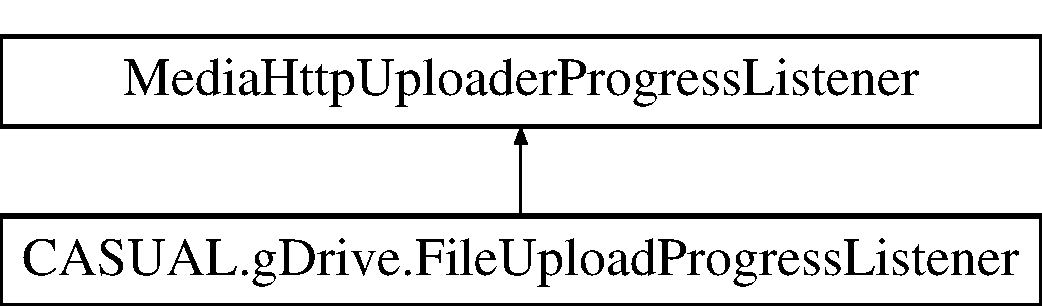
\includegraphics[height=2.000000cm]{classCASUAL_1_1gDrive_1_1FileUploadProgressListener}
\end{center}
\end{figure}
\subsection*{Public Member Functions}
\begin{DoxyCompactItemize}
\item 
\hypertarget{classCASUAL_1_1gDrive_1_1FileUploadProgressListener_a1e60179b7ff0f44a110e1ce7a40dc326}{{\bfseries File\-Upload\-Progress\-Listener} (String name)}\label{classCASUAL_1_1gDrive_1_1FileUploadProgressListener_a1e60179b7ff0f44a110e1ce7a40dc326}

\item 
\hypertarget{classCASUAL_1_1gDrive_1_1FileUploadProgressListener_a107c51afda6bb20d4c5d37710f0c32c3}{void {\bfseries progress\-Changed} (Media\-Http\-Uploader uploader)  throws I\-O\-Exception }\label{classCASUAL_1_1gDrive_1_1FileUploadProgressListener_a107c51afda6bb20d4c5d37710f0c32c3}

\end{DoxyCompactItemize}
\subsection*{Public Attributes}
\begin{DoxyCompactItemize}
\item 
\hypertarget{classCASUAL_1_1gDrive_1_1FileUploadProgressListener_a33f4df4c07281c06bef5d21fc57ccdaa}{\hyperlink{classCASUAL_1_1gDrive_1_1downUpProgress}{down\-Up\-Progress} {\bfseries dlp}}\label{classCASUAL_1_1gDrive_1_1FileUploadProgressListener_a33f4df4c07281c06bef5d21fc57ccdaa}

\end{DoxyCompactItemize}


\subsection{Detailed Description}
\begin{DoxyAuthor}{Author}
loglud 
\end{DoxyAuthor}


The documentation for this class was generated from the following file\-:\begin{DoxyCompactItemize}
\item 
branches/\-Testing\-Branch/\-G\-Doc/src/\-C\-A\-S\-U\-A\-L/g\-Drive/File\-Upload\-Progress\-Listener.\-java\end{DoxyCompactItemize}

\hypertarget{classCASUAL_1_1HeimdallInstall}{\section{C\-A\-S\-U\-A\-L.\-Heimdall\-Install Class Reference}
\label{classCASUAL_1_1HeimdallInstall}\index{C\-A\-S\-U\-A\-L.\-Heimdall\-Install@{C\-A\-S\-U\-A\-L.\-Heimdall\-Install}}
}
\subsection*{Public Member Functions}
\begin{DoxyCompactItemize}
\item 
boolean \hyperlink{classCASUAL_1_1HeimdallInstall_a50633964b1eb9ae286cfaae3d1d288dd}{deploy\-Heimdall\-For\-Windows} ()
\item 
boolean \hyperlink{classCASUAL_1_1HeimdallInstall_aeed58a2f098e237d8532b553824f813d}{check\-Heimdall} ()
\item 
boolean \hyperlink{classCASUAL_1_1HeimdallInstall_a932c3a701a6dd740d2a4171cb3802544}{install\-Heimdall} ()
\item 
boolean \hyperlink{classCASUAL_1_1HeimdallInstall_aaa85ff3b6f6ddf52850fe791db21da15}{install\-Windows\-Drivers} ()
\item 
void \hyperlink{classCASUAL_1_1HeimdallInstall_aa884481a876d8d67c8b48c1252efaae4}{display\-Windows\-Permissions\-Message\-And\-Exit} ()
\item 
boolean \hyperlink{classCASUAL_1_1HeimdallInstall_a7d0022c631eef27a410a08f33b989e1a}{check\-And\-Deploy\-Heimdall} ()
\item 
boolean \hyperlink{classCASUAL_1_1HeimdallInstall_a706906189ba536381bc49d78f5702a25}{check\-Heimdall\-Version} ()
\end{DoxyCompactItemize}
\subsection*{Public Attributes}
\begin{DoxyCompactItemize}
\item 
String \hyperlink{classCASUAL_1_1HeimdallInstall_a5203df5605f1c468861edbacd3cc174d}{V\-I\-D} = \char`\"{}\char`\"{}
\item 
String \hyperlink{classCASUAL_1_1HeimdallInstall_ac8b2b370a75b48ad9efea5740aad4418}{P\-I\-D} = \char`\"{}\char`\"{}
\end{DoxyCompactItemize}


\subsection{Detailed Description}
\begin{DoxyAuthor}{Author}
adam 
\end{DoxyAuthor}


\subsection{Member Function Documentation}
\hypertarget{classCASUAL_1_1HeimdallInstall_a7d0022c631eef27a410a08f33b989e1a}{\index{C\-A\-S\-U\-A\-L\-::\-Heimdall\-Install@{C\-A\-S\-U\-A\-L\-::\-Heimdall\-Install}!check\-And\-Deploy\-Heimdall@{check\-And\-Deploy\-Heimdall}}
\index{check\-And\-Deploy\-Heimdall@{check\-And\-Deploy\-Heimdall}!CASUAL::HeimdallInstall@{C\-A\-S\-U\-A\-L\-::\-Heimdall\-Install}}
\subsubsection[{check\-And\-Deploy\-Heimdall}]{\setlength{\rightskip}{0pt plus 5cm}boolean C\-A\-S\-U\-A\-L.\-Heimdall\-Install.\-check\-And\-Deploy\-Heimdall (
\begin{DoxyParamCaption}
{}
\end{DoxyParamCaption}
)}}\label{classCASUAL_1_1HeimdallInstall_a7d0022c631eef27a410a08f33b989e1a}
checks and deploys heimdall

\begin{DoxyReturn}{Returns}
true if deployed 
\end{DoxyReturn}
\hypertarget{classCASUAL_1_1HeimdallInstall_aeed58a2f098e237d8532b553824f813d}{\index{C\-A\-S\-U\-A\-L\-::\-Heimdall\-Install@{C\-A\-S\-U\-A\-L\-::\-Heimdall\-Install}!check\-Heimdall@{check\-Heimdall}}
\index{check\-Heimdall@{check\-Heimdall}!CASUAL::HeimdallInstall@{C\-A\-S\-U\-A\-L\-::\-Heimdall\-Install}}
\subsubsection[{check\-Heimdall}]{\setlength{\rightskip}{0pt plus 5cm}boolean C\-A\-S\-U\-A\-L.\-Heimdall\-Install.\-check\-Heimdall (
\begin{DoxyParamCaption}
{}
\end{DoxyParamCaption}
)}}\label{classCASUAL_1_1HeimdallInstall_aeed58a2f098e237d8532b553824f813d}
checks if heimdall is deployed

\begin{DoxyReturn}{Returns}
true if heidmall version returns anything 
\end{DoxyReturn}
\hypertarget{classCASUAL_1_1HeimdallInstall_a706906189ba536381bc49d78f5702a25}{\index{C\-A\-S\-U\-A\-L\-::\-Heimdall\-Install@{C\-A\-S\-U\-A\-L\-::\-Heimdall\-Install}!check\-Heimdall\-Version@{check\-Heimdall\-Version}}
\index{check\-Heimdall\-Version@{check\-Heimdall\-Version}!CASUAL::HeimdallInstall@{C\-A\-S\-U\-A\-L\-::\-Heimdall\-Install}}
\subsubsection[{check\-Heimdall\-Version}]{\setlength{\rightskip}{0pt plus 5cm}boolean C\-A\-S\-U\-A\-L.\-Heimdall\-Install.\-check\-Heimdall\-Version (
\begin{DoxyParamCaption}
{}
\end{DoxyParamCaption}
)}}\label{classCASUAL_1_1HeimdallInstall_a706906189ba536381bc49d78f5702a25}
checks the heimdall version against version expected from \hyperlink{classCASUAL_1_1Statics}{Statics}

\begin{DoxyReturn}{Returns}
true if version is good 
\end{DoxyReturn}
\hypertarget{classCASUAL_1_1HeimdallInstall_a50633964b1eb9ae286cfaae3d1d288dd}{\index{C\-A\-S\-U\-A\-L\-::\-Heimdall\-Install@{C\-A\-S\-U\-A\-L\-::\-Heimdall\-Install}!deploy\-Heimdall\-For\-Windows@{deploy\-Heimdall\-For\-Windows}}
\index{deploy\-Heimdall\-For\-Windows@{deploy\-Heimdall\-For\-Windows}!CASUAL::HeimdallInstall@{C\-A\-S\-U\-A\-L\-::\-Heimdall\-Install}}
\subsubsection[{deploy\-Heimdall\-For\-Windows}]{\setlength{\rightskip}{0pt plus 5cm}boolean C\-A\-S\-U\-A\-L.\-Heimdall\-Install.\-deploy\-Heimdall\-For\-Windows (
\begin{DoxyParamCaption}
{}
\end{DoxyParamCaption}
)}}\label{classCASUAL_1_1HeimdallInstall_a50633964b1eb9ae286cfaae3d1d288dd}
deploys heimdal

\begin{DoxyReturn}{Returns}
true if deployed 
\end{DoxyReturn}
\hypertarget{classCASUAL_1_1HeimdallInstall_aa884481a876d8d67c8b48c1252efaae4}{\index{C\-A\-S\-U\-A\-L\-::\-Heimdall\-Install@{C\-A\-S\-U\-A\-L\-::\-Heimdall\-Install}!display\-Windows\-Permissions\-Message\-And\-Exit@{display\-Windows\-Permissions\-Message\-And\-Exit}}
\index{display\-Windows\-Permissions\-Message\-And\-Exit@{display\-Windows\-Permissions\-Message\-And\-Exit}!CASUAL::HeimdallInstall@{C\-A\-S\-U\-A\-L\-::\-Heimdall\-Install}}
\subsubsection[{display\-Windows\-Permissions\-Message\-And\-Exit}]{\setlength{\rightskip}{0pt plus 5cm}void C\-A\-S\-U\-A\-L.\-Heimdall\-Install.\-display\-Windows\-Permissions\-Message\-And\-Exit (
\begin{DoxyParamCaption}
{}
\end{DoxyParamCaption}
)}}\label{classCASUAL_1_1HeimdallInstall_aa884481a876d8d67c8b48c1252efaae4}
displays a message to the user that Windows permissions were not obtainable \hypertarget{classCASUAL_1_1HeimdallInstall_a932c3a701a6dd740d2a4171cb3802544}{\index{C\-A\-S\-U\-A\-L\-::\-Heimdall\-Install@{C\-A\-S\-U\-A\-L\-::\-Heimdall\-Install}!install\-Heimdall@{install\-Heimdall}}
\index{install\-Heimdall@{install\-Heimdall}!CASUAL::HeimdallInstall@{C\-A\-S\-U\-A\-L\-::\-Heimdall\-Install}}
\subsubsection[{install\-Heimdall}]{\setlength{\rightskip}{0pt plus 5cm}boolean C\-A\-S\-U\-A\-L.\-Heimdall\-Install.\-install\-Heimdall (
\begin{DoxyParamCaption}
{}
\end{DoxyParamCaption}
)}}\label{classCASUAL_1_1HeimdallInstall_a932c3a701a6dd740d2a4171cb3802544}
installs heimdall

\begin{DoxyReturn}{Returns}
true if heimdall was detected 
\end{DoxyReturn}
\hypertarget{classCASUAL_1_1HeimdallInstall_aaa85ff3b6f6ddf52850fe791db21da15}{\index{C\-A\-S\-U\-A\-L\-::\-Heimdall\-Install@{C\-A\-S\-U\-A\-L\-::\-Heimdall\-Install}!install\-Windows\-Drivers@{install\-Windows\-Drivers}}
\index{install\-Windows\-Drivers@{install\-Windows\-Drivers}!CASUAL::HeimdallInstall@{C\-A\-S\-U\-A\-L\-::\-Heimdall\-Install}}
\subsubsection[{install\-Windows\-Drivers}]{\setlength{\rightskip}{0pt plus 5cm}boolean C\-A\-S\-U\-A\-L.\-Heimdall\-Install.\-install\-Windows\-Drivers (
\begin{DoxyParamCaption}
{}
\end{DoxyParamCaption}
)}}\label{classCASUAL_1_1HeimdallInstall_aaa85ff3b6f6ddf52850fe791db21da15}
Installs windows drivers

\begin{DoxyReturn}{Returns}
always returns true  always returns true? 
\end{DoxyReturn}


\subsection{Member Data Documentation}
\hypertarget{classCASUAL_1_1HeimdallInstall_ac8b2b370a75b48ad9efea5740aad4418}{\index{C\-A\-S\-U\-A\-L\-::\-Heimdall\-Install@{C\-A\-S\-U\-A\-L\-::\-Heimdall\-Install}!P\-I\-D@{P\-I\-D}}
\index{P\-I\-D@{P\-I\-D}!CASUAL::HeimdallInstall@{C\-A\-S\-U\-A\-L\-::\-Heimdall\-Install}}
\subsubsection[{P\-I\-D}]{\setlength{\rightskip}{0pt plus 5cm}String C\-A\-S\-U\-A\-L.\-Heimdall\-Install.\-P\-I\-D = \char`\"{}\char`\"{}}}\label{classCASUAL_1_1HeimdallInstall_ac8b2b370a75b48ad9efea5740aad4418}
Device I\-D detected \hypertarget{classCASUAL_1_1HeimdallInstall_a5203df5605f1c468861edbacd3cc174d}{\index{C\-A\-S\-U\-A\-L\-::\-Heimdall\-Install@{C\-A\-S\-U\-A\-L\-::\-Heimdall\-Install}!V\-I\-D@{V\-I\-D}}
\index{V\-I\-D@{V\-I\-D}!CASUAL::HeimdallInstall@{C\-A\-S\-U\-A\-L\-::\-Heimdall\-Install}}
\subsubsection[{V\-I\-D}]{\setlength{\rightskip}{0pt plus 5cm}String C\-A\-S\-U\-A\-L.\-Heimdall\-Install.\-V\-I\-D = \char`\"{}\char`\"{}}}\label{classCASUAL_1_1HeimdallInstall_a5203df5605f1c468861edbacd3cc174d}
Vendor I\-D detected 

The documentation for this class was generated from the following file\-:\begin{DoxyCompactItemize}
\item 
trunk/\-C\-A\-S\-U\-A\-Lcore/src/\-C\-A\-S\-U\-A\-L/Heimdall\-Install.\-java\end{DoxyCompactItemize}

\hypertarget{classCASUAL_1_1HeimdallTools}{\section{C\-A\-S\-U\-A\-L.\-Heimdall\-Tools Class Reference}
\label{classCASUAL_1_1HeimdallTools}\index{C\-A\-S\-U\-A\-L.\-Heimdall\-Tools@{C\-A\-S\-U\-A\-L.\-Heimdall\-Tools}}
}
\subsection*{Public Member Functions}
\begin{DoxyCompactItemize}
\item 
void \hyperlink{classCASUAL_1_1HeimdallTools_af64f9e031d33e50778af32a812eb2188}{do\-Heimdall\-Wait\-For\-Device} ()
\item 
String \hyperlink{classCASUAL_1_1HeimdallTools_af06559bcbdf984cb99d7d0a2490e8bb6}{do\-Elevated\-Heimdall\-Shell\-Command} ()
\item 
String \hyperlink{classCASUAL_1_1HeimdallTools_ad9817f83a5a51de3e1a11c3a561ca10e}{do\-Heimdall\-Shell\-Command} ()
\item 
String \hyperlink{classCASUAL_1_1HeimdallTools_a08c2dafb0094c3c867bcb3188a5170f3}{did\-Heimdall\-Error} (String std\-Err\-Log)
\end{DoxyCompactItemize}
\subsection*{Static Public Member Functions}
\begin{DoxyCompactItemize}
\item 
static String \hyperlink{classCASUAL_1_1HeimdallTools_a2a78a83cbc516c7a801e4212b71cc925}{get\-Heimdall\-Command} ()
\end{DoxyCompactItemize}


\subsection{Detailed Description}
\begin{DoxyAuthor}{Author}
adam 
\end{DoxyAuthor}


\subsection{Member Function Documentation}
\hypertarget{classCASUAL_1_1HeimdallTools_a08c2dafb0094c3c867bcb3188a5170f3}{\index{C\-A\-S\-U\-A\-L\-::\-Heimdall\-Tools@{C\-A\-S\-U\-A\-L\-::\-Heimdall\-Tools}!did\-Heimdall\-Error@{did\-Heimdall\-Error}}
\index{did\-Heimdall\-Error@{did\-Heimdall\-Error}!CASUAL::HeimdallTools@{C\-A\-S\-U\-A\-L\-::\-Heimdall\-Tools}}
\subsubsection[{did\-Heimdall\-Error}]{\setlength{\rightskip}{0pt plus 5cm}String C\-A\-S\-U\-A\-L.\-Heimdall\-Tools.\-did\-Heimdall\-Error (
\begin{DoxyParamCaption}
\item[{String}]{std\-Err\-Log}
\end{DoxyParamCaption}
)}}\label{classCASUAL_1_1HeimdallTools_a08c2dafb0094c3c867bcb3188a5170f3}
checks if Heimdall threw an error


\begin{DoxyParams}{Parameters}
{\em std\-Err\-Log} & \hyperlink{namespaceCASUAL}{C\-A\-S\-U\-A\-L} log output \\
\hline
\end{DoxyParams}
\begin{DoxyReturn}{Returns}
containing halted if cannot continue or continue if it can
\end{DoxyReturn}
\begin{DoxyAuthor}{Author}
Jeremy Loper \href{mailto:jrloper@gmail.com}{\tt jrloper@gmail.\-com} 
\end{DoxyAuthor}
\hypertarget{classCASUAL_1_1HeimdallTools_af06559bcbdf984cb99d7d0a2490e8bb6}{\index{C\-A\-S\-U\-A\-L\-::\-Heimdall\-Tools@{C\-A\-S\-U\-A\-L\-::\-Heimdall\-Tools}!do\-Elevated\-Heimdall\-Shell\-Command@{do\-Elevated\-Heimdall\-Shell\-Command}}
\index{do\-Elevated\-Heimdall\-Shell\-Command@{do\-Elevated\-Heimdall\-Shell\-Command}!CASUAL::HeimdallTools@{C\-A\-S\-U\-A\-L\-::\-Heimdall\-Tools}}
\subsubsection[{do\-Elevated\-Heimdall\-Shell\-Command}]{\setlength{\rightskip}{0pt plus 5cm}String C\-A\-S\-U\-A\-L.\-Heimdall\-Tools.\-do\-Elevated\-Heimdall\-Shell\-Command (
\begin{DoxyParamCaption}
{}
\end{DoxyParamCaption}
)}}\label{classCASUAL_1_1HeimdallTools_af06559bcbdf984cb99d7d0a2490e8bb6}
performs an elevated heimdall command

\begin{DoxyReturn}{Returns}
result from heimdall 
\end{DoxyReturn}
\hypertarget{classCASUAL_1_1HeimdallTools_ad9817f83a5a51de3e1a11c3a561ca10e}{\index{C\-A\-S\-U\-A\-L\-::\-Heimdall\-Tools@{C\-A\-S\-U\-A\-L\-::\-Heimdall\-Tools}!do\-Heimdall\-Shell\-Command@{do\-Heimdall\-Shell\-Command}}
\index{do\-Heimdall\-Shell\-Command@{do\-Heimdall\-Shell\-Command}!CASUAL::HeimdallTools@{C\-A\-S\-U\-A\-L\-::\-Heimdall\-Tools}}
\subsubsection[{do\-Heimdall\-Shell\-Command}]{\setlength{\rightskip}{0pt plus 5cm}String C\-A\-S\-U\-A\-L.\-Heimdall\-Tools.\-do\-Heimdall\-Shell\-Command (
\begin{DoxyParamCaption}
{}
\end{DoxyParamCaption}
)}}\label{classCASUAL_1_1HeimdallTools_ad9817f83a5a51de3e1a11c3a561ca10e}
performs a heimdall command

\begin{DoxyReturn}{Returns}
value from heimdall command 
\end{DoxyReturn}
\hypertarget{classCASUAL_1_1HeimdallTools_af64f9e031d33e50778af32a812eb2188}{\index{C\-A\-S\-U\-A\-L\-::\-Heimdall\-Tools@{C\-A\-S\-U\-A\-L\-::\-Heimdall\-Tools}!do\-Heimdall\-Wait\-For\-Device@{do\-Heimdall\-Wait\-For\-Device}}
\index{do\-Heimdall\-Wait\-For\-Device@{do\-Heimdall\-Wait\-For\-Device}!CASUAL::HeimdallTools@{C\-A\-S\-U\-A\-L\-::\-Heimdall\-Tools}}
\subsubsection[{do\-Heimdall\-Wait\-For\-Device}]{\setlength{\rightskip}{0pt plus 5cm}void C\-A\-S\-U\-A\-L.\-Heimdall\-Tools.\-do\-Heimdall\-Wait\-For\-Device (
\begin{DoxyParamCaption}
{}
\end{DoxyParamCaption}
)}}\label{classCASUAL_1_1HeimdallTools_af64f9e031d33e50778af32a812eb2188}
do nothing until a heimdall device is detected \hypertarget{classCASUAL_1_1HeimdallTools_a2a78a83cbc516c7a801e4212b71cc925}{\index{C\-A\-S\-U\-A\-L\-::\-Heimdall\-Tools@{C\-A\-S\-U\-A\-L\-::\-Heimdall\-Tools}!get\-Heimdall\-Command@{get\-Heimdall\-Command}}
\index{get\-Heimdall\-Command@{get\-Heimdall\-Command}!CASUAL::HeimdallTools@{C\-A\-S\-U\-A\-L\-::\-Heimdall\-Tools}}
\subsubsection[{get\-Heimdall\-Command}]{\setlength{\rightskip}{0pt plus 5cm}static String C\-A\-S\-U\-A\-L.\-Heimdall\-Tools.\-get\-Heimdall\-Command (
\begin{DoxyParamCaption}
{}
\end{DoxyParamCaption}
)\hspace{0.3cm}{\ttfamily [static]}}}\label{classCASUAL_1_1HeimdallTools_a2a78a83cbc516c7a801e4212b71cc925}
gets the command to run heimdall

\begin{DoxyReturn}{Returns}
string path to heimdall 
\end{DoxyReturn}


The documentation for this class was generated from the following file\-:\begin{DoxyCompactItemize}
\item 
trunk/\-C\-A\-S\-U\-A\-Lcore/src/\-C\-A\-S\-U\-A\-L/Heimdall\-Tools.\-java\end{DoxyCompactItemize}

\hypertarget{interfaceCASUAL_1_1iCASUALGUI}{\section{C\-A\-S\-U\-A\-L.\-i\-C\-A\-S\-U\-A\-L\-G\-U\-I Interface Reference}
\label{interfaceCASUAL_1_1iCASUALGUI}\index{C\-A\-S\-U\-A\-L.\-i\-C\-A\-S\-U\-A\-L\-G\-U\-I@{C\-A\-S\-U\-A\-L.\-i\-C\-A\-S\-U\-A\-L\-G\-U\-I}}
}
Inheritance diagram for C\-A\-S\-U\-A\-L.\-i\-C\-A\-S\-U\-A\-L\-G\-U\-I\-:\begin{figure}[H]
\begin{center}
\leavevmode
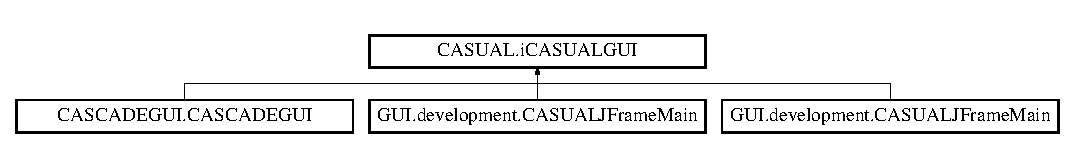
\includegraphics[height=1.555556cm]{interfaceCASUAL_1_1iCASUALGUI}
\end{center}
\end{figure}
\subsection*{Public Member Functions}
\begin{DoxyCompactItemize}
\item 
void \hyperlink{interfaceCASUAL_1_1iCASUALGUI_aaae0a373aee8f7939993f184f0cc8b5a}{dispose} ()
\item 
void \hyperlink{interfaceCASUAL_1_1iCASUALGUI_aca8a0966823e8e2c2c8fdb88d20c73bb}{Start\-Button\-Action\-Performed} ()
\item 
String \hyperlink{interfaceCASUAL_1_1iCASUALGUI_a842659e4a515bdb9558082d0f1232f30}{combo\-Box\-Get\-Selected\-Item} ()
\item 
void \hyperlink{interfaceCASUAL_1_1iCASUALGUI_a27a26714a3f630a69be0138fa8393979}{combo\-Box\-Script\-Selector\-Add\-New\-Item} (String item)
\item 
boolean \hyperlink{interfaceCASUAL_1_1iCASUALGUI_a13e5b49519aeda6e1df10ae7680cded9}{enable\-Controls} (boolean status)
\item 
boolean \hyperlink{interfaceCASUAL_1_1iCASUALGUI_a0da22163bda8a58af87b464429dc3386}{get\-Control\-Status} ()
\item 
void \hyperlink{interfaceCASUAL_1_1iCASUALGUI_ad929e91c437aeb24548442633974d220}{set\-C\-A\-S\-P\-A\-C} (\hyperlink{classCASUAL_1_1caspac_1_1Caspac}{Caspac} caspac)
\item 
void \hyperlink{interfaceCASUAL_1_1iCASUALGUI_a3d7accd1069c78528f99e124ce67c399}{set\-Information\-Scroll\-Border\-Text} (String title)
\item 
void \hyperlink{interfaceCASUAL_1_1iCASUALGUI_a7b198a07d16f4f48b39afce9ef721c6e}{set\-Progress\-Bar} (int value)
\item 
void \hyperlink{interfaceCASUAL_1_1iCASUALGUI_afc569857a9e6df91758381d0efdf76e0}{set\-Progress\-Bar\-Max} (int value)
\item 
void \hyperlink{interfaceCASUAL_1_1iCASUALGUI_a98ace169d3438ca1b2c29828bc720040}{set\-Script} (\hyperlink{classCASUAL_1_1caspac_1_1Script}{Script} s)
\item 
void \hyperlink{interfaceCASUAL_1_1iCASUALGUI_ae53420dc6cfc3169e2b9e1ef0baea5f0}{set\-Start\-Button\-Text} (String text)
\item 
void \hyperlink{interfaceCASUAL_1_1iCASUALGUI_aa7560d79744afd442b110512202a10a1}{set\-Status\-Label\-Icon} (String Icon, String Text)
\item 
void \hyperlink{interfaceCASUAL_1_1iCASUALGUI_a584c6b63237727f8420ac25374cfcd30}{set\-Status\-Message\-Label} (String text)
\item 
void \hyperlink{interfaceCASUAL_1_1iCASUALGUI_ab40b2bd85be375159b9e764f53f185ec}{set\-Window\-Banner\-Image} (Buffered\-Image icon, String text)
\item 
void \hyperlink{interfaceCASUAL_1_1iCASUALGUI_a4f23768f43fa4cfe9b6bfce1b9cedb6d}{set\-Window\-Banner\-Text} (String text)
\item 
void \hyperlink{interfaceCASUAL_1_1iCASUALGUI_a94783dbf5d258d8a5bb516d03fba14f8}{set\-Visible} (boolean b)
\item 
void \hyperlink{interfaceCASUAL_1_1iCASUALGUI_a1d118a6e2fa316d2a1e90256a0572795}{device\-Connected} (String mode)
\item 
void \hyperlink{interfaceCASUAL_1_1iCASUALGUI_a360c068814d6714ff427d2bced13c6d2}{device\-Disconnected} ()
\item 
void \hyperlink{interfaceCASUAL_1_1iCASUALGUI_a14f848e7113fb3488549d5c00bd9e751}{device\-Multiple\-Connected} (int number\-Of\-Devices\-Connected)
\item 
void \hyperlink{interfaceCASUAL_1_1iCASUALGUI_a601a31c3779aaf519ce85b77cc2ca753}{notification\-Permissions\-Required} ()
\item 
void \hyperlink{interfaceCASUAL_1_1iCASUALGUI_a8ed1e2eeb8018c79935326542fbe66e7}{notification\-C\-A\-S\-U\-A\-L\-Sound} ()
\item 
void \hyperlink{interfaceCASUAL_1_1iCASUALGUI_aadb0d6eaf13ea440f2fde52635686aba}{notification\-Input\-Requested} ()
\item 
void \hyperlink{interfaceCASUAL_1_1iCASUALGUI_afb18773fbee213dccef143061f8d8b32}{notification\-General} ()
\item 
void \hyperlink{interfaceCASUAL_1_1iCASUALGUI_ab7b99ad8c318f392a4d757239c25b773}{notification\-Request\-To\-Continue} ()
\item 
void \hyperlink{interfaceCASUAL_1_1iCASUALGUI_a840b79c54833bb3292f227b2d8244d17}{notification\-User\-Action\-Is\-Required} ()
\end{DoxyCompactItemize}


\subsection{Detailed Description}
\begin{DoxyAuthor}{Author}
adam 
\end{DoxyAuthor}


\subsection{Member Function Documentation}
\hypertarget{interfaceCASUAL_1_1iCASUALGUI_a842659e4a515bdb9558082d0f1232f30}{\index{C\-A\-S\-U\-A\-L\-::i\-C\-A\-S\-U\-A\-L\-G\-U\-I@{C\-A\-S\-U\-A\-L\-::i\-C\-A\-S\-U\-A\-L\-G\-U\-I}!combo\-Box\-Get\-Selected\-Item@{combo\-Box\-Get\-Selected\-Item}}
\index{combo\-Box\-Get\-Selected\-Item@{combo\-Box\-Get\-Selected\-Item}!CASUAL::iCASUALGUI@{C\-A\-S\-U\-A\-L\-::i\-C\-A\-S\-U\-A\-L\-G\-U\-I}}
\subsubsection[{combo\-Box\-Get\-Selected\-Item}]{\setlength{\rightskip}{0pt plus 5cm}String C\-A\-S\-U\-A\-L.\-i\-C\-A\-S\-U\-A\-L\-G\-U\-I.\-combo\-Box\-Get\-Selected\-Item (
\begin{DoxyParamCaption}
{}
\end{DoxyParamCaption}
)}}\label{interfaceCASUAL_1_1iCASUALGUI_a842659e4a515bdb9558082d0f1232f30}
gets the selected combobox item.

\begin{DoxyReturn}{Returns}
selected item in combobox 
\end{DoxyReturn}


Implemented in \hyperlink{classCASCADEGUI_1_1CASCADEGUI_af25dc89641d2fda0b73830594ba30b2d}{C\-A\-S\-C\-A\-D\-E\-G\-U\-I.\-C\-A\-S\-C\-A\-D\-E\-G\-U\-I}, \hyperlink{classGUI_1_1development_1_1CASUALJFrameMain_a65473b796550f93cd0a64fbdc008e321}{G\-U\-I.\-development.\-C\-A\-S\-U\-A\-L\-J\-Frame\-Main}, and \hyperlink{classGUI_1_1development_1_1CASUALJFrameMain_a65473b796550f93cd0a64fbdc008e321}{G\-U\-I.\-development.\-C\-A\-S\-U\-A\-L\-J\-Frame\-Main}.

\hypertarget{interfaceCASUAL_1_1iCASUALGUI_a27a26714a3f630a69be0138fa8393979}{\index{C\-A\-S\-U\-A\-L\-::i\-C\-A\-S\-U\-A\-L\-G\-U\-I@{C\-A\-S\-U\-A\-L\-::i\-C\-A\-S\-U\-A\-L\-G\-U\-I}!combo\-Box\-Script\-Selector\-Add\-New\-Item@{combo\-Box\-Script\-Selector\-Add\-New\-Item}}
\index{combo\-Box\-Script\-Selector\-Add\-New\-Item@{combo\-Box\-Script\-Selector\-Add\-New\-Item}!CASUAL::iCASUALGUI@{C\-A\-S\-U\-A\-L\-::i\-C\-A\-S\-U\-A\-L\-G\-U\-I}}
\subsubsection[{combo\-Box\-Script\-Selector\-Add\-New\-Item}]{\setlength{\rightskip}{0pt plus 5cm}void C\-A\-S\-U\-A\-L.\-i\-C\-A\-S\-U\-A\-L\-G\-U\-I.\-combo\-Box\-Script\-Selector\-Add\-New\-Item (
\begin{DoxyParamCaption}
\item[{String}]{item}
\end{DoxyParamCaption}
)}}\label{interfaceCASUAL_1_1iCASUALGUI_a27a26714a3f630a69be0138fa8393979}
adds an item to the combo box


\begin{DoxyParams}{Parameters}
{\em item} & item to add \\
\hline
\end{DoxyParams}


Implemented in \hyperlink{classCASCADEGUI_1_1CASCADEGUI_a1813e3b344e699edfa6ff6fb732fd602}{C\-A\-S\-C\-A\-D\-E\-G\-U\-I.\-C\-A\-S\-C\-A\-D\-E\-G\-U\-I}, \hyperlink{classGUI_1_1development_1_1CASUALJFrameMain_ad67026cebd68aaa9d5e50a1d772e890b}{G\-U\-I.\-development.\-C\-A\-S\-U\-A\-L\-J\-Frame\-Main}, and \hyperlink{classGUI_1_1development_1_1CASUALJFrameMain_ad67026cebd68aaa9d5e50a1d772e890b}{G\-U\-I.\-development.\-C\-A\-S\-U\-A\-L\-J\-Frame\-Main}.

\hypertarget{interfaceCASUAL_1_1iCASUALGUI_a1d118a6e2fa316d2a1e90256a0572795}{\index{C\-A\-S\-U\-A\-L\-::i\-C\-A\-S\-U\-A\-L\-G\-U\-I@{C\-A\-S\-U\-A\-L\-::i\-C\-A\-S\-U\-A\-L\-G\-U\-I}!device\-Connected@{device\-Connected}}
\index{device\-Connected@{device\-Connected}!CASUAL::iCASUALGUI@{C\-A\-S\-U\-A\-L\-::i\-C\-A\-S\-U\-A\-L\-G\-U\-I}}
\subsubsection[{device\-Connected}]{\setlength{\rightskip}{0pt plus 5cm}void C\-A\-S\-U\-A\-L.\-i\-C\-A\-S\-U\-A\-L\-G\-U\-I.\-device\-Connected (
\begin{DoxyParamCaption}
\item[{String}]{mode}
\end{DoxyParamCaption}
)}}\label{interfaceCASUAL_1_1iCASUALGUI_a1d118a6e2fa316d2a1e90256a0572795}
called when device is connected 
\begin{DoxyParams}{Parameters}
{\em mode} & adb/fastboot/heimdall/flashtool \\
\hline
\end{DoxyParams}


Implemented in \hyperlink{classCASCADEGUI_1_1CASCADEGUI_a82d1be792b2be3a60e57fd7dd67a1900}{C\-A\-S\-C\-A\-D\-E\-G\-U\-I.\-C\-A\-S\-C\-A\-D\-E\-G\-U\-I}, \hyperlink{classGUI_1_1development_1_1CASUALJFrameMain_aacdbe72ec60c691bc5606c3893a52f7d}{G\-U\-I.\-development.\-C\-A\-S\-U\-A\-L\-J\-Frame\-Main}, and \hyperlink{classGUI_1_1development_1_1CASUALJFrameMain_aacdbe72ec60c691bc5606c3893a52f7d}{G\-U\-I.\-development.\-C\-A\-S\-U\-A\-L\-J\-Frame\-Main}.

\hypertarget{interfaceCASUAL_1_1iCASUALGUI_a360c068814d6714ff427d2bced13c6d2}{\index{C\-A\-S\-U\-A\-L\-::i\-C\-A\-S\-U\-A\-L\-G\-U\-I@{C\-A\-S\-U\-A\-L\-::i\-C\-A\-S\-U\-A\-L\-G\-U\-I}!device\-Disconnected@{device\-Disconnected}}
\index{device\-Disconnected@{device\-Disconnected}!CASUAL::iCASUALGUI@{C\-A\-S\-U\-A\-L\-::i\-C\-A\-S\-U\-A\-L\-G\-U\-I}}
\subsubsection[{device\-Disconnected}]{\setlength{\rightskip}{0pt plus 5cm}void C\-A\-S\-U\-A\-L.\-i\-C\-A\-S\-U\-A\-L\-G\-U\-I.\-device\-Disconnected (
\begin{DoxyParamCaption}
{}
\end{DoxyParamCaption}
)}}\label{interfaceCASUAL_1_1iCASUALGUI_a360c068814d6714ff427d2bced13c6d2}
Device has disconnected, alert the user 

Implemented in \hyperlink{classCASCADEGUI_1_1CASCADEGUI_a3aed3d6c9d77c7ca52f07137ce41f2a6}{C\-A\-S\-C\-A\-D\-E\-G\-U\-I.\-C\-A\-S\-C\-A\-D\-E\-G\-U\-I}, \hyperlink{classGUI_1_1development_1_1CASUALJFrameMain_abd52217ac3134fd45343dd6838601f38}{G\-U\-I.\-development.\-C\-A\-S\-U\-A\-L\-J\-Frame\-Main}, and \hyperlink{classGUI_1_1development_1_1CASUALJFrameMain_abd52217ac3134fd45343dd6838601f38}{G\-U\-I.\-development.\-C\-A\-S\-U\-A\-L\-J\-Frame\-Main}.

\hypertarget{interfaceCASUAL_1_1iCASUALGUI_a14f848e7113fb3488549d5c00bd9e751}{\index{C\-A\-S\-U\-A\-L\-::i\-C\-A\-S\-U\-A\-L\-G\-U\-I@{C\-A\-S\-U\-A\-L\-::i\-C\-A\-S\-U\-A\-L\-G\-U\-I}!device\-Multiple\-Connected@{device\-Multiple\-Connected}}
\index{device\-Multiple\-Connected@{device\-Multiple\-Connected}!CASUAL::iCASUALGUI@{C\-A\-S\-U\-A\-L\-::i\-C\-A\-S\-U\-A\-L\-G\-U\-I}}
\subsubsection[{device\-Multiple\-Connected}]{\setlength{\rightskip}{0pt plus 5cm}void C\-A\-S\-U\-A\-L.\-i\-C\-A\-S\-U\-A\-L\-G\-U\-I.\-device\-Multiple\-Connected (
\begin{DoxyParamCaption}
\item[{int}]{number\-Of\-Devices\-Connected}
\end{DoxyParamCaption}
)}}\label{interfaceCASUAL_1_1iCASUALGUI_a14f848e7113fb3488549d5c00bd9e751}
multiple devices are detected. only one is allowed 
\begin{DoxyParams}{Parameters}
{\em number\-Of\-Devices\-Connected} & number of devices \\
\hline
\end{DoxyParams}


Implemented in \hyperlink{classCASCADEGUI_1_1CASCADEGUI_a7be4ced04beac7bf4439daa7d0ba8e16}{C\-A\-S\-C\-A\-D\-E\-G\-U\-I.\-C\-A\-S\-C\-A\-D\-E\-G\-U\-I}, \hyperlink{classGUI_1_1development_1_1CASUALJFrameMain_a0bc8b9c2ca823527932c53d869174e90}{G\-U\-I.\-development.\-C\-A\-S\-U\-A\-L\-J\-Frame\-Main}, and \hyperlink{classGUI_1_1development_1_1CASUALJFrameMain_a0bc8b9c2ca823527932c53d869174e90}{G\-U\-I.\-development.\-C\-A\-S\-U\-A\-L\-J\-Frame\-Main}.

\hypertarget{interfaceCASUAL_1_1iCASUALGUI_aaae0a373aee8f7939993f184f0cc8b5a}{\index{C\-A\-S\-U\-A\-L\-::i\-C\-A\-S\-U\-A\-L\-G\-U\-I@{C\-A\-S\-U\-A\-L\-::i\-C\-A\-S\-U\-A\-L\-G\-U\-I}!dispose@{dispose}}
\index{dispose@{dispose}!CASUAL::iCASUALGUI@{C\-A\-S\-U\-A\-L\-::i\-C\-A\-S\-U\-A\-L\-G\-U\-I}}
\subsubsection[{dispose}]{\setlength{\rightskip}{0pt plus 5cm}void C\-A\-S\-U\-A\-L.\-i\-C\-A\-S\-U\-A\-L\-G\-U\-I.\-dispose (
\begin{DoxyParamCaption}
{}
\end{DoxyParamCaption}
)}}\label{interfaceCASUAL_1_1iCASUALGUI_aaae0a373aee8f7939993f184f0cc8b5a}
disposes the current window. should be used to terminate application. \hypertarget{interfaceCASUAL_1_1iCASUALGUI_a13e5b49519aeda6e1df10ae7680cded9}{\index{C\-A\-S\-U\-A\-L\-::i\-C\-A\-S\-U\-A\-L\-G\-U\-I@{C\-A\-S\-U\-A\-L\-::i\-C\-A\-S\-U\-A\-L\-G\-U\-I}!enable\-Controls@{enable\-Controls}}
\index{enable\-Controls@{enable\-Controls}!CASUAL::iCASUALGUI@{C\-A\-S\-U\-A\-L\-::i\-C\-A\-S\-U\-A\-L\-G\-U\-I}}
\subsubsection[{enable\-Controls}]{\setlength{\rightskip}{0pt plus 5cm}boolean C\-A\-S\-U\-A\-L.\-i\-C\-A\-S\-U\-A\-L\-G\-U\-I.\-enable\-Controls (
\begin{DoxyParamCaption}
\item[{boolean}]{status}
\end{DoxyParamCaption}
)}}\label{interfaceCASUAL_1_1iCASUALGUI_a13e5b49519aeda6e1df10ae7680cded9}
sets controls status


\begin{DoxyParams}{Parameters}
{\em status} & commanded value \\
\hline
\end{DoxyParams}
\begin{DoxyReturn}{Returns}
true if enabled false if not 
\end{DoxyReturn}


Implemented in \hyperlink{classCASCADEGUI_1_1CASCADEGUI_ac4c6bac7bbe7bdfdd74aba69571e2ee0}{C\-A\-S\-C\-A\-D\-E\-G\-U\-I.\-C\-A\-S\-C\-A\-D\-E\-G\-U\-I}, \hyperlink{classGUI_1_1development_1_1CASUALJFrameMain_ae8a8f3e56ff374c6274633ed621dc815}{G\-U\-I.\-development.\-C\-A\-S\-U\-A\-L\-J\-Frame\-Main}, and \hyperlink{classGUI_1_1development_1_1CASUALJFrameMain_ae8a8f3e56ff374c6274633ed621dc815}{G\-U\-I.\-development.\-C\-A\-S\-U\-A\-L\-J\-Frame\-Main}.

\hypertarget{interfaceCASUAL_1_1iCASUALGUI_a0da22163bda8a58af87b464429dc3386}{\index{C\-A\-S\-U\-A\-L\-::i\-C\-A\-S\-U\-A\-L\-G\-U\-I@{C\-A\-S\-U\-A\-L\-::i\-C\-A\-S\-U\-A\-L\-G\-U\-I}!get\-Control\-Status@{get\-Control\-Status}}
\index{get\-Control\-Status@{get\-Control\-Status}!CASUAL::iCASUALGUI@{C\-A\-S\-U\-A\-L\-::i\-C\-A\-S\-U\-A\-L\-G\-U\-I}}
\subsubsection[{get\-Control\-Status}]{\setlength{\rightskip}{0pt plus 5cm}boolean C\-A\-S\-U\-A\-L.\-i\-C\-A\-S\-U\-A\-L\-G\-U\-I.\-get\-Control\-Status (
\begin{DoxyParamCaption}
{}
\end{DoxyParamCaption}
)}}\label{interfaceCASUAL_1_1iCASUALGUI_a0da22163bda8a58af87b464429dc3386}
gets the control status

\begin{DoxyReturn}{Returns}
true if enabled 
\end{DoxyReturn}


Implemented in \hyperlink{classCASCADEGUI_1_1CASCADEGUI_a4a473942292f9a51f057d128b62910d6}{C\-A\-S\-C\-A\-D\-E\-G\-U\-I.\-C\-A\-S\-C\-A\-D\-E\-G\-U\-I}, \hyperlink{classGUI_1_1development_1_1CASUALJFrameMain_af0f386b4ecdf89d6eaa43dc78cd4f6ef}{G\-U\-I.\-development.\-C\-A\-S\-U\-A\-L\-J\-Frame\-Main}, and \hyperlink{classGUI_1_1development_1_1CASUALJFrameMain_af0f386b4ecdf89d6eaa43dc78cd4f6ef}{G\-U\-I.\-development.\-C\-A\-S\-U\-A\-L\-J\-Frame\-Main}.

\hypertarget{interfaceCASUAL_1_1iCASUALGUI_a8ed1e2eeb8018c79935326542fbe66e7}{\index{C\-A\-S\-U\-A\-L\-::i\-C\-A\-S\-U\-A\-L\-G\-U\-I@{C\-A\-S\-U\-A\-L\-::i\-C\-A\-S\-U\-A\-L\-G\-U\-I}!notification\-C\-A\-S\-U\-A\-L\-Sound@{notification\-C\-A\-S\-U\-A\-L\-Sound}}
\index{notification\-C\-A\-S\-U\-A\-L\-Sound@{notification\-C\-A\-S\-U\-A\-L\-Sound}!CASUAL::iCASUALGUI@{C\-A\-S\-U\-A\-L\-::i\-C\-A\-S\-U\-A\-L\-G\-U\-I}}
\subsubsection[{notification\-C\-A\-S\-U\-A\-L\-Sound}]{\setlength{\rightskip}{0pt plus 5cm}void C\-A\-S\-U\-A\-L.\-i\-C\-A\-S\-U\-A\-L\-G\-U\-I.\-notification\-C\-A\-S\-U\-A\-L\-Sound (
\begin{DoxyParamCaption}
{}
\end{DoxyParamCaption}
)}}\label{interfaceCASUAL_1_1iCASUALGUI_a8ed1e2eeb8018c79935326542fbe66e7}
Startup event 

Implemented in \hyperlink{classCASCADEGUI_1_1CASCADEGUI_ab626397400af7582d19e7200daba1678}{C\-A\-S\-C\-A\-D\-E\-G\-U\-I.\-C\-A\-S\-C\-A\-D\-E\-G\-U\-I}, \hyperlink{classGUI_1_1development_1_1CASUALJFrameMain_a4450abb55d30b94308914af44ef4ee98}{G\-U\-I.\-development.\-C\-A\-S\-U\-A\-L\-J\-Frame\-Main}, and \hyperlink{classGUI_1_1development_1_1CASUALJFrameMain_a4450abb55d30b94308914af44ef4ee98}{G\-U\-I.\-development.\-C\-A\-S\-U\-A\-L\-J\-Frame\-Main}.

\hypertarget{interfaceCASUAL_1_1iCASUALGUI_afb18773fbee213dccef143061f8d8b32}{\index{C\-A\-S\-U\-A\-L\-::i\-C\-A\-S\-U\-A\-L\-G\-U\-I@{C\-A\-S\-U\-A\-L\-::i\-C\-A\-S\-U\-A\-L\-G\-U\-I}!notification\-General@{notification\-General}}
\index{notification\-General@{notification\-General}!CASUAL::iCASUALGUI@{C\-A\-S\-U\-A\-L\-::i\-C\-A\-S\-U\-A\-L\-G\-U\-I}}
\subsubsection[{notification\-General}]{\setlength{\rightskip}{0pt plus 5cm}void C\-A\-S\-U\-A\-L.\-i\-C\-A\-S\-U\-A\-L\-G\-U\-I.\-notification\-General (
\begin{DoxyParamCaption}
{}
\end{DoxyParamCaption}
)}}\label{interfaceCASUAL_1_1iCASUALGUI_afb18773fbee213dccef143061f8d8b32}
A notification has been issued to the user 

Implemented in \hyperlink{classCASCADEGUI_1_1CASCADEGUI_a00033dc3bbee0c1cc56930758e951b99}{C\-A\-S\-C\-A\-D\-E\-G\-U\-I.\-C\-A\-S\-C\-A\-D\-E\-G\-U\-I}, \hyperlink{classGUI_1_1development_1_1CASUALJFrameMain_a1fe1b03a2ad5aa30c5c8fe208813d4f6}{G\-U\-I.\-development.\-C\-A\-S\-U\-A\-L\-J\-Frame\-Main}, and \hyperlink{classGUI_1_1development_1_1CASUALJFrameMain_a1fe1b03a2ad5aa30c5c8fe208813d4f6}{G\-U\-I.\-development.\-C\-A\-S\-U\-A\-L\-J\-Frame\-Main}.

\hypertarget{interfaceCASUAL_1_1iCASUALGUI_aadb0d6eaf13ea440f2fde52635686aba}{\index{C\-A\-S\-U\-A\-L\-::i\-C\-A\-S\-U\-A\-L\-G\-U\-I@{C\-A\-S\-U\-A\-L\-::i\-C\-A\-S\-U\-A\-L\-G\-U\-I}!notification\-Input\-Requested@{notification\-Input\-Requested}}
\index{notification\-Input\-Requested@{notification\-Input\-Requested}!CASUAL::iCASUALGUI@{C\-A\-S\-U\-A\-L\-::i\-C\-A\-S\-U\-A\-L\-G\-U\-I}}
\subsubsection[{notification\-Input\-Requested}]{\setlength{\rightskip}{0pt plus 5cm}void C\-A\-S\-U\-A\-L.\-i\-C\-A\-S\-U\-A\-L\-G\-U\-I.\-notification\-Input\-Requested (
\begin{DoxyParamCaption}
{}
\end{DoxyParamCaption}
)}}\label{interfaceCASUAL_1_1iCASUALGUI_aadb0d6eaf13ea440f2fde52635686aba}
Input is requested from the user 

Implemented in \hyperlink{classCASCADEGUI_1_1CASCADEGUI_a39f374e0ad4f250b0018ad111f59c1d9}{C\-A\-S\-C\-A\-D\-E\-G\-U\-I.\-C\-A\-S\-C\-A\-D\-E\-G\-U\-I}, \hyperlink{classGUI_1_1development_1_1CASUALJFrameMain_a34444561be5204262b95aa6001c4aac1}{G\-U\-I.\-development.\-C\-A\-S\-U\-A\-L\-J\-Frame\-Main}, and \hyperlink{classGUI_1_1development_1_1CASUALJFrameMain_a34444561be5204262b95aa6001c4aac1}{G\-U\-I.\-development.\-C\-A\-S\-U\-A\-L\-J\-Frame\-Main}.

\hypertarget{interfaceCASUAL_1_1iCASUALGUI_a601a31c3779aaf519ce85b77cc2ca753}{\index{C\-A\-S\-U\-A\-L\-::i\-C\-A\-S\-U\-A\-L\-G\-U\-I@{C\-A\-S\-U\-A\-L\-::i\-C\-A\-S\-U\-A\-L\-G\-U\-I}!notification\-Permissions\-Required@{notification\-Permissions\-Required}}
\index{notification\-Permissions\-Required@{notification\-Permissions\-Required}!CASUAL::iCASUALGUI@{C\-A\-S\-U\-A\-L\-::i\-C\-A\-S\-U\-A\-L\-G\-U\-I}}
\subsubsection[{notification\-Permissions\-Required}]{\setlength{\rightskip}{0pt plus 5cm}void C\-A\-S\-U\-A\-L.\-i\-C\-A\-S\-U\-A\-L\-G\-U\-I.\-notification\-Permissions\-Required (
\begin{DoxyParamCaption}
{}
\end{DoxyParamCaption}
)}}\label{interfaceCASUAL_1_1iCASUALGUI_a601a31c3779aaf519ce85b77cc2ca753}
permissions escillation is required 

Implemented in \hyperlink{classCASCADEGUI_1_1CASCADEGUI_ab0416903e989b65c33122f4ec0c31523}{C\-A\-S\-C\-A\-D\-E\-G\-U\-I.\-C\-A\-S\-C\-A\-D\-E\-G\-U\-I}, \hyperlink{classGUI_1_1development_1_1CASUALJFrameMain_a798bd91756d5c27d6f5017a8025b4130}{G\-U\-I.\-development.\-C\-A\-S\-U\-A\-L\-J\-Frame\-Main}, and \hyperlink{classGUI_1_1development_1_1CASUALJFrameMain_a798bd91756d5c27d6f5017a8025b4130}{G\-U\-I.\-development.\-C\-A\-S\-U\-A\-L\-J\-Frame\-Main}.

\hypertarget{interfaceCASUAL_1_1iCASUALGUI_ab7b99ad8c318f392a4d757239c25b773}{\index{C\-A\-S\-U\-A\-L\-::i\-C\-A\-S\-U\-A\-L\-G\-U\-I@{C\-A\-S\-U\-A\-L\-::i\-C\-A\-S\-U\-A\-L\-G\-U\-I}!notification\-Request\-To\-Continue@{notification\-Request\-To\-Continue}}
\index{notification\-Request\-To\-Continue@{notification\-Request\-To\-Continue}!CASUAL::iCASUALGUI@{C\-A\-S\-U\-A\-L\-::i\-C\-A\-S\-U\-A\-L\-G\-U\-I}}
\subsubsection[{notification\-Request\-To\-Continue}]{\setlength{\rightskip}{0pt plus 5cm}void C\-A\-S\-U\-A\-L.\-i\-C\-A\-S\-U\-A\-L\-G\-U\-I.\-notification\-Request\-To\-Continue (
\begin{DoxyParamCaption}
{}
\end{DoxyParamCaption}
)}}\label{interfaceCASUAL_1_1iCASUALGUI_ab7b99ad8c318f392a4d757239c25b773}
a request to continue has been issued to the user 

Implemented in \hyperlink{classCASCADEGUI_1_1CASCADEGUI_a814bf0111d304835ec958df02ad61da3}{C\-A\-S\-C\-A\-D\-E\-G\-U\-I.\-C\-A\-S\-C\-A\-D\-E\-G\-U\-I}, \hyperlink{classGUI_1_1development_1_1CASUALJFrameMain_ad90ba0f96765dfa612ccb92cccecbe98}{G\-U\-I.\-development.\-C\-A\-S\-U\-A\-L\-J\-Frame\-Main}, and \hyperlink{classGUI_1_1development_1_1CASUALJFrameMain_ad90ba0f96765dfa612ccb92cccecbe98}{G\-U\-I.\-development.\-C\-A\-S\-U\-A\-L\-J\-Frame\-Main}.

\hypertarget{interfaceCASUAL_1_1iCASUALGUI_a840b79c54833bb3292f227b2d8244d17}{\index{C\-A\-S\-U\-A\-L\-::i\-C\-A\-S\-U\-A\-L\-G\-U\-I@{C\-A\-S\-U\-A\-L\-::i\-C\-A\-S\-U\-A\-L\-G\-U\-I}!notification\-User\-Action\-Is\-Required@{notification\-User\-Action\-Is\-Required}}
\index{notification\-User\-Action\-Is\-Required@{notification\-User\-Action\-Is\-Required}!CASUAL::iCASUALGUI@{C\-A\-S\-U\-A\-L\-::i\-C\-A\-S\-U\-A\-L\-G\-U\-I}}
\subsubsection[{notification\-User\-Action\-Is\-Required}]{\setlength{\rightskip}{0pt plus 5cm}void C\-A\-S\-U\-A\-L.\-i\-C\-A\-S\-U\-A\-L\-G\-U\-I.\-notification\-User\-Action\-Is\-Required (
\begin{DoxyParamCaption}
{}
\end{DoxyParamCaption}
)}}\label{interfaceCASUAL_1_1iCASUALGUI_a840b79c54833bb3292f227b2d8244d17}
User action is required 

Implemented in \hyperlink{classCASCADEGUI_1_1CASCADEGUI_aba49e61e74bc16729356ec7199e9b4be}{C\-A\-S\-C\-A\-D\-E\-G\-U\-I.\-C\-A\-S\-C\-A\-D\-E\-G\-U\-I}, \hyperlink{classGUI_1_1development_1_1CASUALJFrameMain_a442ecb84833fd7e90fbe97fcb3feb1e7}{G\-U\-I.\-development.\-C\-A\-S\-U\-A\-L\-J\-Frame\-Main}, and \hyperlink{classGUI_1_1development_1_1CASUALJFrameMain_a442ecb84833fd7e90fbe97fcb3feb1e7}{G\-U\-I.\-development.\-C\-A\-S\-U\-A\-L\-J\-Frame\-Main}.

\hypertarget{interfaceCASUAL_1_1iCASUALGUI_ad929e91c437aeb24548442633974d220}{\index{C\-A\-S\-U\-A\-L\-::i\-C\-A\-S\-U\-A\-L\-G\-U\-I@{C\-A\-S\-U\-A\-L\-::i\-C\-A\-S\-U\-A\-L\-G\-U\-I}!set\-C\-A\-S\-P\-A\-C@{set\-C\-A\-S\-P\-A\-C}}
\index{set\-C\-A\-S\-P\-A\-C@{set\-C\-A\-S\-P\-A\-C}!CASUAL::iCASUALGUI@{C\-A\-S\-U\-A\-L\-::i\-C\-A\-S\-U\-A\-L\-G\-U\-I}}
\subsubsection[{set\-C\-A\-S\-P\-A\-C}]{\setlength{\rightskip}{0pt plus 5cm}void C\-A\-S\-U\-A\-L.\-i\-C\-A\-S\-U\-A\-L\-G\-U\-I.\-set\-C\-A\-S\-P\-A\-C (
\begin{DoxyParamCaption}
\item[{{\bf Caspac}}]{caspac}
\end{DoxyParamCaption}
)}}\label{interfaceCASUAL_1_1iCASUALGUI_ad929e91c437aeb24548442633974d220}
Sets a reference to the current C\-A\-S\-P\-A\-C so information can be displayed 
\begin{DoxyParams}{Parameters}
{\em caspac} & caspac to reference \\
\hline
\end{DoxyParams}


Implemented in \hyperlink{classCASCADEGUI_1_1CASCADEGUI_aac14a58f86200f7e55e2223db8a7b5d8}{C\-A\-S\-C\-A\-D\-E\-G\-U\-I.\-C\-A\-S\-C\-A\-D\-E\-G\-U\-I}, \hyperlink{classGUI_1_1development_1_1CASUALJFrameMain_ae49b006965b1e155a86c6c8c7aec1ecb}{G\-U\-I.\-development.\-C\-A\-S\-U\-A\-L\-J\-Frame\-Main}, and \hyperlink{classGUI_1_1development_1_1CASUALJFrameMain_ae49b006965b1e155a86c6c8c7aec1ecb}{G\-U\-I.\-development.\-C\-A\-S\-U\-A\-L\-J\-Frame\-Main}.

\hypertarget{interfaceCASUAL_1_1iCASUALGUI_a3d7accd1069c78528f99e124ce67c399}{\index{C\-A\-S\-U\-A\-L\-::i\-C\-A\-S\-U\-A\-L\-G\-U\-I@{C\-A\-S\-U\-A\-L\-::i\-C\-A\-S\-U\-A\-L\-G\-U\-I}!set\-Information\-Scroll\-Border\-Text@{set\-Information\-Scroll\-Border\-Text}}
\index{set\-Information\-Scroll\-Border\-Text@{set\-Information\-Scroll\-Border\-Text}!CASUAL::iCASUALGUI@{C\-A\-S\-U\-A\-L\-::i\-C\-A\-S\-U\-A\-L\-G\-U\-I}}
\subsubsection[{set\-Information\-Scroll\-Border\-Text}]{\setlength{\rightskip}{0pt plus 5cm}void C\-A\-S\-U\-A\-L.\-i\-C\-A\-S\-U\-A\-L\-G\-U\-I.\-set\-Information\-Scroll\-Border\-Text (
\begin{DoxyParamCaption}
\item[{String}]{title}
\end{DoxyParamCaption}
)}}\label{interfaceCASUAL_1_1iCASUALGUI_a3d7accd1069c78528f99e124ce67c399}
Sets the current status of the window. 
\begin{DoxyParams}{Parameters}
{\em title} & current status \\
\hline
\end{DoxyParams}


Implemented in \hyperlink{classCASCADEGUI_1_1CASCADEGUI_a105553c3bb3dbadac14672993160cb1e}{C\-A\-S\-C\-A\-D\-E\-G\-U\-I.\-C\-A\-S\-C\-A\-D\-E\-G\-U\-I}, \hyperlink{classGUI_1_1development_1_1CASUALJFrameMain_aa715222603235cd4c0e10ccf8ec35c64}{G\-U\-I.\-development.\-C\-A\-S\-U\-A\-L\-J\-Frame\-Main}, and \hyperlink{classGUI_1_1development_1_1CASUALJFrameMain_aa715222603235cd4c0e10ccf8ec35c64}{G\-U\-I.\-development.\-C\-A\-S\-U\-A\-L\-J\-Frame\-Main}.

\hypertarget{interfaceCASUAL_1_1iCASUALGUI_a7b198a07d16f4f48b39afce9ef721c6e}{\index{C\-A\-S\-U\-A\-L\-::i\-C\-A\-S\-U\-A\-L\-G\-U\-I@{C\-A\-S\-U\-A\-L\-::i\-C\-A\-S\-U\-A\-L\-G\-U\-I}!set\-Progress\-Bar@{set\-Progress\-Bar}}
\index{set\-Progress\-Bar@{set\-Progress\-Bar}!CASUAL::iCASUALGUI@{C\-A\-S\-U\-A\-L\-::i\-C\-A\-S\-U\-A\-L\-G\-U\-I}}
\subsubsection[{set\-Progress\-Bar}]{\setlength{\rightskip}{0pt plus 5cm}void C\-A\-S\-U\-A\-L.\-i\-C\-A\-S\-U\-A\-L\-G\-U\-I.\-set\-Progress\-Bar (
\begin{DoxyParamCaption}
\item[{int}]{value}
\end{DoxyParamCaption}
)}}\label{interfaceCASUAL_1_1iCASUALGUI_a7b198a07d16f4f48b39afce9ef721c6e}
sets the progress bar value.


\begin{DoxyParams}{Parameters}
{\em value} & value for progress bar \\
\hline
\end{DoxyParams}


Implemented in \hyperlink{classCASCADEGUI_1_1CASCADEGUI_adb2973646bf59367a782ad933bc86c60}{C\-A\-S\-C\-A\-D\-E\-G\-U\-I.\-C\-A\-S\-C\-A\-D\-E\-G\-U\-I}, \hyperlink{classGUI_1_1development_1_1CASUALJFrameMain_ab5a2bd6f9960330e92ec832a037d8475}{G\-U\-I.\-development.\-C\-A\-S\-U\-A\-L\-J\-Frame\-Main}, and \hyperlink{classGUI_1_1development_1_1CASUALJFrameMain_ab5a2bd6f9960330e92ec832a037d8475}{G\-U\-I.\-development.\-C\-A\-S\-U\-A\-L\-J\-Frame\-Main}.

\hypertarget{interfaceCASUAL_1_1iCASUALGUI_afc569857a9e6df91758381d0efdf76e0}{\index{C\-A\-S\-U\-A\-L\-::i\-C\-A\-S\-U\-A\-L\-G\-U\-I@{C\-A\-S\-U\-A\-L\-::i\-C\-A\-S\-U\-A\-L\-G\-U\-I}!set\-Progress\-Bar\-Max@{set\-Progress\-Bar\-Max}}
\index{set\-Progress\-Bar\-Max@{set\-Progress\-Bar\-Max}!CASUAL::iCASUALGUI@{C\-A\-S\-U\-A\-L\-::i\-C\-A\-S\-U\-A\-L\-G\-U\-I}}
\subsubsection[{set\-Progress\-Bar\-Max}]{\setlength{\rightskip}{0pt plus 5cm}void C\-A\-S\-U\-A\-L.\-i\-C\-A\-S\-U\-A\-L\-G\-U\-I.\-set\-Progress\-Bar\-Max (
\begin{DoxyParamCaption}
\item[{int}]{value}
\end{DoxyParamCaption}
)}}\label{interfaceCASUAL_1_1iCASUALGUI_afc569857a9e6df91758381d0efdf76e0}
sets max value for progress bar


\begin{DoxyParams}{Parameters}
{\em value} & maximum \\
\hline
\end{DoxyParams}


Implemented in \hyperlink{classCASCADEGUI_1_1CASCADEGUI_a2c09183b7f524fda208305ad72ac05ef}{C\-A\-S\-C\-A\-D\-E\-G\-U\-I.\-C\-A\-S\-C\-A\-D\-E\-G\-U\-I}, \hyperlink{classGUI_1_1development_1_1CASUALJFrameMain_aea01e24b1f4fd89b0b362527eb07bc9b}{G\-U\-I.\-development.\-C\-A\-S\-U\-A\-L\-J\-Frame\-Main}, and \hyperlink{classGUI_1_1development_1_1CASUALJFrameMain_aea01e24b1f4fd89b0b362527eb07bc9b}{G\-U\-I.\-development.\-C\-A\-S\-U\-A\-L\-J\-Frame\-Main}.

\hypertarget{interfaceCASUAL_1_1iCASUALGUI_a98ace169d3438ca1b2c29828bc720040}{\index{C\-A\-S\-U\-A\-L\-::i\-C\-A\-S\-U\-A\-L\-G\-U\-I@{C\-A\-S\-U\-A\-L\-::i\-C\-A\-S\-U\-A\-L\-G\-U\-I}!set\-Script@{set\-Script}}
\index{set\-Script@{set\-Script}!CASUAL::iCASUALGUI@{C\-A\-S\-U\-A\-L\-::i\-C\-A\-S\-U\-A\-L\-G\-U\-I}}
\subsubsection[{set\-Script}]{\setlength{\rightskip}{0pt plus 5cm}void C\-A\-S\-U\-A\-L.\-i\-C\-A\-S\-U\-A\-L\-G\-U\-I.\-set\-Script (
\begin{DoxyParamCaption}
\item[{{\bf Script}}]{s}
\end{DoxyParamCaption}
)}}\label{interfaceCASUAL_1_1iCASUALGUI_a98ace169d3438ca1b2c29828bc720040}
Sets the active script for the window 
\begin{DoxyParams}{Parameters}
{\em s} & script which is now active \\
\hline
\end{DoxyParams}


Implemented in \hyperlink{classCASCADEGUI_1_1CASCADEGUI_a6b753ecf736bbae2c6781c927f997eb4}{C\-A\-S\-C\-A\-D\-E\-G\-U\-I.\-C\-A\-S\-C\-A\-D\-E\-G\-U\-I}, \hyperlink{classGUI_1_1development_1_1CASUALJFrameMain_a5c63c8abc79e383d5ebf1d38c4dfcd13}{G\-U\-I.\-development.\-C\-A\-S\-U\-A\-L\-J\-Frame\-Main}, and \hyperlink{classGUI_1_1development_1_1CASUALJFrameMain_a5c63c8abc79e383d5ebf1d38c4dfcd13}{G\-U\-I.\-development.\-C\-A\-S\-U\-A\-L\-J\-Frame\-Main}.

\hypertarget{interfaceCASUAL_1_1iCASUALGUI_ae53420dc6cfc3169e2b9e1ef0baea5f0}{\index{C\-A\-S\-U\-A\-L\-::i\-C\-A\-S\-U\-A\-L\-G\-U\-I@{C\-A\-S\-U\-A\-L\-::i\-C\-A\-S\-U\-A\-L\-G\-U\-I}!set\-Start\-Button\-Text@{set\-Start\-Button\-Text}}
\index{set\-Start\-Button\-Text@{set\-Start\-Button\-Text}!CASUAL::iCASUALGUI@{C\-A\-S\-U\-A\-L\-::i\-C\-A\-S\-U\-A\-L\-G\-U\-I}}
\subsubsection[{set\-Start\-Button\-Text}]{\setlength{\rightskip}{0pt plus 5cm}void C\-A\-S\-U\-A\-L.\-i\-C\-A\-S\-U\-A\-L\-G\-U\-I.\-set\-Start\-Button\-Text (
\begin{DoxyParamCaption}
\item[{String}]{text}
\end{DoxyParamCaption}
)}}\label{interfaceCASUAL_1_1iCASUALGUI_ae53420dc6cfc3169e2b9e1ef0baea5f0}
sets \char`\"{}do it!\char`\"{} button text


\begin{DoxyParams}{Parameters}
{\em text} & text for main execution button \\
\hline
\end{DoxyParams}


Implemented in \hyperlink{classCASCADEGUI_1_1CASCADEGUI_a4ac6e6fe72d4de88c0ea75c92b9ef6e7}{C\-A\-S\-C\-A\-D\-E\-G\-U\-I.\-C\-A\-S\-C\-A\-D\-E\-G\-U\-I}, \hyperlink{classGUI_1_1development_1_1CASUALJFrameMain_a9e5b6e12ea7e3967c9f628788e3bc860}{G\-U\-I.\-development.\-C\-A\-S\-U\-A\-L\-J\-Frame\-Main}, and \hyperlink{classGUI_1_1development_1_1CASUALJFrameMain_a9e5b6e12ea7e3967c9f628788e3bc860}{G\-U\-I.\-development.\-C\-A\-S\-U\-A\-L\-J\-Frame\-Main}.

\hypertarget{interfaceCASUAL_1_1iCASUALGUI_aa7560d79744afd442b110512202a10a1}{\index{C\-A\-S\-U\-A\-L\-::i\-C\-A\-S\-U\-A\-L\-G\-U\-I@{C\-A\-S\-U\-A\-L\-::i\-C\-A\-S\-U\-A\-L\-G\-U\-I}!set\-Status\-Label\-Icon@{set\-Status\-Label\-Icon}}
\index{set\-Status\-Label\-Icon@{set\-Status\-Label\-Icon}!CASUAL::iCASUALGUI@{C\-A\-S\-U\-A\-L\-::i\-C\-A\-S\-U\-A\-L\-G\-U\-I}}
\subsubsection[{set\-Status\-Label\-Icon}]{\setlength{\rightskip}{0pt plus 5cm}void C\-A\-S\-U\-A\-L.\-i\-C\-A\-S\-U\-A\-L\-G\-U\-I.\-set\-Status\-Label\-Icon (
\begin{DoxyParamCaption}
\item[{String}]{Icon, }
\item[{String}]{Text}
\end{DoxyParamCaption}
)}}\label{interfaceCASUAL_1_1iCASUALGUI_aa7560d79744afd442b110512202a10a1}
changes the label icon


\begin{DoxyParams}{Parameters}
{\em Icon} & resource to be displayed \\
\hline
{\em Text} & text if icon is missing \\
\hline
\end{DoxyParams}


Implemented in \hyperlink{classCASCADEGUI_1_1CASCADEGUI_ab81a942be6a431984e2b8a3c64fa721b}{C\-A\-S\-C\-A\-D\-E\-G\-U\-I.\-C\-A\-S\-C\-A\-D\-E\-G\-U\-I}, \hyperlink{classGUI_1_1development_1_1CASUALJFrameMain_a6abde49bfe2650f447b5c6abc7d6f077}{G\-U\-I.\-development.\-C\-A\-S\-U\-A\-L\-J\-Frame\-Main}, and \hyperlink{classGUI_1_1development_1_1CASUALJFrameMain_a6abde49bfe2650f447b5c6abc7d6f077}{G\-U\-I.\-development.\-C\-A\-S\-U\-A\-L\-J\-Frame\-Main}.

\hypertarget{interfaceCASUAL_1_1iCASUALGUI_a584c6b63237727f8420ac25374cfcd30}{\index{C\-A\-S\-U\-A\-L\-::i\-C\-A\-S\-U\-A\-L\-G\-U\-I@{C\-A\-S\-U\-A\-L\-::i\-C\-A\-S\-U\-A\-L\-G\-U\-I}!set\-Status\-Message\-Label@{set\-Status\-Message\-Label}}
\index{set\-Status\-Message\-Label@{set\-Status\-Message\-Label}!CASUAL::iCASUALGUI@{C\-A\-S\-U\-A\-L\-::i\-C\-A\-S\-U\-A\-L\-G\-U\-I}}
\subsubsection[{set\-Status\-Message\-Label}]{\setlength{\rightskip}{0pt plus 5cm}void C\-A\-S\-U\-A\-L.\-i\-C\-A\-S\-U\-A\-L\-G\-U\-I.\-set\-Status\-Message\-Label (
\begin{DoxyParamCaption}
\item[{String}]{text}
\end{DoxyParamCaption}
)}}\label{interfaceCASUAL_1_1iCASUALGUI_a584c6b63237727f8420ac25374cfcd30}
sets the message label text


\begin{DoxyParams}{Parameters}
{\em text} & label text \\
\hline
\end{DoxyParams}


Implemented in \hyperlink{classCASCADEGUI_1_1CASCADEGUI_a85d7babb514ed1c760779538fcb666a9}{C\-A\-S\-C\-A\-D\-E\-G\-U\-I.\-C\-A\-S\-C\-A\-D\-E\-G\-U\-I}, \hyperlink{classGUI_1_1development_1_1CASUALJFrameMain_ad655b0e480491023e7ad25af422c95a9}{G\-U\-I.\-development.\-C\-A\-S\-U\-A\-L\-J\-Frame\-Main}, and \hyperlink{classGUI_1_1development_1_1CASUALJFrameMain_ad655b0e480491023e7ad25af422c95a9}{G\-U\-I.\-development.\-C\-A\-S\-U\-A\-L\-J\-Frame\-Main}.

\hypertarget{interfaceCASUAL_1_1iCASUALGUI_a94783dbf5d258d8a5bb516d03fba14f8}{\index{C\-A\-S\-U\-A\-L\-::i\-C\-A\-S\-U\-A\-L\-G\-U\-I@{C\-A\-S\-U\-A\-L\-::i\-C\-A\-S\-U\-A\-L\-G\-U\-I}!set\-Visible@{set\-Visible}}
\index{set\-Visible@{set\-Visible}!CASUAL::iCASUALGUI@{C\-A\-S\-U\-A\-L\-::i\-C\-A\-S\-U\-A\-L\-G\-U\-I}}
\subsubsection[{set\-Visible}]{\setlength{\rightskip}{0pt plus 5cm}void C\-A\-S\-U\-A\-L.\-i\-C\-A\-S\-U\-A\-L\-G\-U\-I.\-set\-Visible (
\begin{DoxyParamCaption}
\item[{boolean}]{b}
\end{DoxyParamCaption}
)}}\label{interfaceCASUAL_1_1iCASUALGUI_a94783dbf5d258d8a5bb516d03fba14f8}
sets the window visibility 
\begin{DoxyParams}{Parameters}
{\em b} & true if visibility is commanded \\
\hline
\end{DoxyParams}
\hypertarget{interfaceCASUAL_1_1iCASUALGUI_ab40b2bd85be375159b9e764f53f185ec}{\index{C\-A\-S\-U\-A\-L\-::i\-C\-A\-S\-U\-A\-L\-G\-U\-I@{C\-A\-S\-U\-A\-L\-::i\-C\-A\-S\-U\-A\-L\-G\-U\-I}!set\-Window\-Banner\-Image@{set\-Window\-Banner\-Image}}
\index{set\-Window\-Banner\-Image@{set\-Window\-Banner\-Image}!CASUAL::iCASUALGUI@{C\-A\-S\-U\-A\-L\-::i\-C\-A\-S\-U\-A\-L\-G\-U\-I}}
\subsubsection[{set\-Window\-Banner\-Image}]{\setlength{\rightskip}{0pt plus 5cm}void C\-A\-S\-U\-A\-L.\-i\-C\-A\-S\-U\-A\-L\-G\-U\-I.\-set\-Window\-Banner\-Image (
\begin{DoxyParamCaption}
\item[{Buffered\-Image}]{icon, }
\item[{String}]{text}
\end{DoxyParamCaption}
)}}\label{interfaceCASUAL_1_1iCASUALGUI_ab40b2bd85be375159b9e764f53f185ec}
sets window banner image


\begin{DoxyParams}{Parameters}
{\em icon} & image to display \\
\hline
{\em text} & text if image cannot be displayed\\
\hline
{\em icon} & \\
\hline
{\em text} & \\
\hline
\end{DoxyParams}


Implemented in \hyperlink{classCASCADEGUI_1_1CASCADEGUI_a824ff8fb59f84bc3f048f0288796d75e}{C\-A\-S\-C\-A\-D\-E\-G\-U\-I.\-C\-A\-S\-C\-A\-D\-E\-G\-U\-I}, \hyperlink{classGUI_1_1development_1_1CASUALJFrameMain_a61c6f0a35b429a38f63317e05afaf921}{G\-U\-I.\-development.\-C\-A\-S\-U\-A\-L\-J\-Frame\-Main}, and \hyperlink{classGUI_1_1development_1_1CASUALJFrameMain_a61c6f0a35b429a38f63317e05afaf921}{G\-U\-I.\-development.\-C\-A\-S\-U\-A\-L\-J\-Frame\-Main}.

\hypertarget{interfaceCASUAL_1_1iCASUALGUI_a4f23768f43fa4cfe9b6bfce1b9cedb6d}{\index{C\-A\-S\-U\-A\-L\-::i\-C\-A\-S\-U\-A\-L\-G\-U\-I@{C\-A\-S\-U\-A\-L\-::i\-C\-A\-S\-U\-A\-L\-G\-U\-I}!set\-Window\-Banner\-Text@{set\-Window\-Banner\-Text}}
\index{set\-Window\-Banner\-Text@{set\-Window\-Banner\-Text}!CASUAL::iCASUALGUI@{C\-A\-S\-U\-A\-L\-::i\-C\-A\-S\-U\-A\-L\-G\-U\-I}}
\subsubsection[{set\-Window\-Banner\-Text}]{\setlength{\rightskip}{0pt plus 5cm}void C\-A\-S\-U\-A\-L.\-i\-C\-A\-S\-U\-A\-L\-G\-U\-I.\-set\-Window\-Banner\-Text (
\begin{DoxyParamCaption}
\item[{String}]{text}
\end{DoxyParamCaption}
)}}\label{interfaceCASUAL_1_1iCASUALGUI_a4f23768f43fa4cfe9b6bfce1b9cedb6d}
sets the main window banner text if an image is not used


\begin{DoxyParams}{Parameters}
{\em text} & text to display as banner \\
\hline
\end{DoxyParams}


Implemented in \hyperlink{classCASCADEGUI_1_1CASCADEGUI_a80c9fe66dd68d134dc13759c2a757d74}{C\-A\-S\-C\-A\-D\-E\-G\-U\-I.\-C\-A\-S\-C\-A\-D\-E\-G\-U\-I}, \hyperlink{classGUI_1_1development_1_1CASUALJFrameMain_ab21ac8cd692ec2a63ae0339bb68e374e}{G\-U\-I.\-development.\-C\-A\-S\-U\-A\-L\-J\-Frame\-Main}, and \hyperlink{classGUI_1_1development_1_1CASUALJFrameMain_ab21ac8cd692ec2a63ae0339bb68e374e}{G\-U\-I.\-development.\-C\-A\-S\-U\-A\-L\-J\-Frame\-Main}.

\hypertarget{interfaceCASUAL_1_1iCASUALGUI_aca8a0966823e8e2c2c8fdb88d20c73bb}{\index{C\-A\-S\-U\-A\-L\-::i\-C\-A\-S\-U\-A\-L\-G\-U\-I@{C\-A\-S\-U\-A\-L\-::i\-C\-A\-S\-U\-A\-L\-G\-U\-I}!Start\-Button\-Action\-Performed@{Start\-Button\-Action\-Performed}}
\index{Start\-Button\-Action\-Performed@{Start\-Button\-Action\-Performed}!CASUAL::iCASUALGUI@{C\-A\-S\-U\-A\-L\-::i\-C\-A\-S\-U\-A\-L\-G\-U\-I}}
\subsubsection[{Start\-Button\-Action\-Performed}]{\setlength{\rightskip}{0pt plus 5cm}void C\-A\-S\-U\-A\-L.\-i\-C\-A\-S\-U\-A\-L\-G\-U\-I.\-Start\-Button\-Action\-Performed (
\begin{DoxyParamCaption}
{}
\end{DoxyParamCaption}
)}}\label{interfaceCASUAL_1_1iCASUALGUI_aca8a0966823e8e2c2c8fdb88d20c73bb}
the start button was pressed. 

Implemented in \hyperlink{classCASCADEGUI_1_1CASCADEGUI_a0b56a081d828cd896d81278086a55871}{C\-A\-S\-C\-A\-D\-E\-G\-U\-I.\-C\-A\-S\-C\-A\-D\-E\-G\-U\-I}, \hyperlink{classGUI_1_1development_1_1CASUALJFrameMain_a019f07e0dcd01688f121d01a6a4f08fb}{G\-U\-I.\-development.\-C\-A\-S\-U\-A\-L\-J\-Frame\-Main}, and \hyperlink{classGUI_1_1development_1_1CASUALJFrameMain_a019f07e0dcd01688f121d01a6a4f08fb}{G\-U\-I.\-development.\-C\-A\-S\-U\-A\-L\-J\-Frame\-Main}.



The documentation for this interface was generated from the following file\-:\begin{DoxyCompactItemize}
\item 
trunk/\-C\-A\-S\-U\-A\-Lcore/src/\-C\-A\-S\-U\-A\-L/i\-C\-A\-S\-U\-A\-L\-G\-U\-I.\-java\end{DoxyCompactItemize}

\hypertarget{interfaceCASUAL_1_1iCASUALInteraction}{\section{C\-A\-S\-U\-A\-L.\-i\-C\-A\-S\-U\-A\-L\-Interaction Interface Reference}
\label{interfaceCASUAL_1_1iCASUALInteraction}\index{C\-A\-S\-U\-A\-L.\-i\-C\-A\-S\-U\-A\-L\-Interaction@{C\-A\-S\-U\-A\-L.\-i\-C\-A\-S\-U\-A\-L\-Interaction}}
}
Inheritance diagram for C\-A\-S\-U\-A\-L.\-i\-C\-A\-S\-U\-A\-L\-Interaction\-:\begin{figure}[H]
\begin{center}
\leavevmode
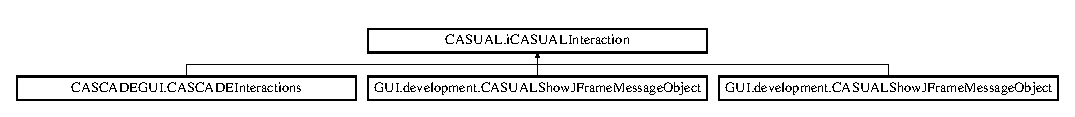
\includegraphics[height=1.127895cm]{interfaceCASUAL_1_1iCASUALInteraction}
\end{center}
\end{figure}
\subsection*{Public Member Functions}
\begin{DoxyCompactItemize}
\item 
String \hyperlink{interfaceCASUAL_1_1iCASUALInteraction_a8c6697fd276aa8519caff45131c14bf4}{display\-Message} (\hyperlink{classCASUAL_1_1CASUALMessageObject}{C\-A\-S\-U\-A\-L\-Message\-Object} message\-Object)
\end{DoxyCompactItemize}
\subsection*{Public Attributes}
\begin{DoxyCompactItemize}
\item 
final int \hyperlink{interfaceCASUAL_1_1iCASUALInteraction_ad8a93fbf136514ec2abf7042846bf8d8}{I\-N\-T\-E\-R\-A\-C\-T\-I\-O\-N\-\_\-\-T\-I\-M\-E\-\_\-\-O\-U\-T} = 0
\item 
final int \hyperlink{interfaceCASUAL_1_1iCASUALInteraction_a9cb2accb41f6b2de8f8076cda916924f}{I\-N\-T\-E\-R\-A\-C\-T\-I\-O\-N\-\_\-\-A\-C\-T\-I\-O\-N\-\_\-\-R\-E\-U\-I\-R\-E\-D} = 1
\item 
final int \hyperlink{interfaceCASUAL_1_1iCASUALInteraction_ab172a9affe078a64623627dc1ef6dcab}{I\-N\-T\-E\-R\-A\-C\-T\-I\-O\-N\-\_\-\-U\-S\-E\-R\-\_\-\-C\-A\-N\-C\-E\-L\-\_\-\-O\-P\-T\-I\-O\-N} = 2
\item 
final int \hyperlink{interfaceCASUAL_1_1iCASUALInteraction_aee60fbef84821ccb93b8508720af91e9}{I\-N\-T\-E\-R\-A\-C\-T\-I\-O\-N\-\_\-\-U\-S\-E\-R\-\_\-\-N\-O\-T\-I\-F\-I\-C\-A\-T\-I\-O\-N} = 3
\item 
final int \hyperlink{interfaceCASUAL_1_1iCASUALInteraction_a88a985d1905b2af7cfa06932e1019346}{I\-N\-T\-E\-R\-A\-C\-T\-I\-O\-N\-\_\-\-S\-H\-O\-W\-\_\-\-I\-N\-F\-O\-R\-M\-A\-T\-I\-O\-N} = 4
\item 
final int \hyperlink{interfaceCASUAL_1_1iCASUALInteraction_aaf019b0daffee32f5c487ee69a0c2886}{I\-N\-T\-E\-R\-A\-C\-T\-I\-O\-N\-\_\-\-S\-H\-O\-W\-\_\-\-E\-R\-R\-O\-R} = 5
\item 
final int \hyperlink{interfaceCASUAL_1_1iCASUALInteraction_aa943e8a9c4f74899de6071e708fe7fdb}{I\-N\-T\-E\-R\-A\-C\-T\-I\-O\-N\-\_\-\-S\-H\-O\-W\-\_\-\-Y\-E\-S\-\_\-\-N\-O} = 6
\item 
final int \hyperlink{interfaceCASUAL_1_1iCASUALInteraction_a96a9320c51af617e4bef953bb055c244}{I\-N\-T\-E\-R\-A\-C\-T\-I\-O\-N\-\_\-\-I\-N\-P\-U\-T\-\_\-\-D\-I\-A\-L\-O\-G} = 7
\item 
final int \hyperlink{interfaceCASUAL_1_1iCASUALInteraction_a7e7889527c716356d3df6039c1aae7c7}{I\-N\-T\-E\-R\-A\-C\-T\-I\-O\-N\-\_\-\-C\-O\-M\-M\-A\-N\-D\-\_\-\-N\-O\-T\-I\-F\-I\-C\-A\-T\-I\-O\-N} = 8
\end{DoxyCompactItemize}


\subsection{Detailed Description}
\hyperlink{interfaceCASUAL_1_1iCASUALInteraction}{i\-C\-A\-S\-U\-A\-L\-Interaction} is a class which provides a means of handling C\-A\-S\-U\-A\-L\-Message\-Objects. The intent is to abstract the \hyperlink{namespaceCASUAL}{C\-A\-S\-U\-A\-L} Messaging System using this class so a developer may implement their own G\-U\-I using any means they like. This class provides notifications which will halt the progress of the script and present information to the user. This allows the user to interact with \hyperlink{namespaceCASUAL}{C\-A\-S\-U\-A\-L}.

In order to change the Messaging A\-P\-I for \hyperlink{namespaceCASUAL}{C\-A\-S\-U\-A\-L}, there is a static reference which is located in C\-A\-S\-U\-A\-L.\-resources.\-C\-A\-S\-U\-A\-L\-App.\-properties the property name change required is Application.\-interactions. This should match the desired class which can handle C\-A\-S\-U\-A\-L\-Message\-Objects

It is recommended that any class implementing \hyperlink{interfaceCASUAL_1_1iCASUALInteraction}{i\-C\-A\-S\-U\-A\-L\-Interaction} handle the following items at a minimum\-:
\begin{DoxyEnumerate}
\item C\-A\-S\-U\-A\-L\-Message\-Object.\-message\-Text
\item $\ast$ C\-A\-S\-U\-A\-L\-Message\-Object.\-title
\end{DoxyEnumerate}

The return value for any \hyperlink{namespaceCASUAL}{C\-A\-S\-U\-A\-L} Message Object aside from those which execute commmands or specifically state they return string results\-: 0-\/ yes, ok, continue 1-\/ no, cancel, stop

\begin{DoxyAuthor}{Author}
adam 
\end{DoxyAuthor}


\subsection{Member Function Documentation}
\hypertarget{interfaceCASUAL_1_1iCASUALInteraction_a8c6697fd276aa8519caff45131c14bf4}{\index{C\-A\-S\-U\-A\-L\-::i\-C\-A\-S\-U\-A\-L\-Interaction@{C\-A\-S\-U\-A\-L\-::i\-C\-A\-S\-U\-A\-L\-Interaction}!display\-Message@{display\-Message}}
\index{display\-Message@{display\-Message}!CASUAL::iCASUALInteraction@{C\-A\-S\-U\-A\-L\-::i\-C\-A\-S\-U\-A\-L\-Interaction}}
\subsubsection[{display\-Message}]{\setlength{\rightskip}{0pt plus 5cm}String C\-A\-S\-U\-A\-L.\-i\-C\-A\-S\-U\-A\-L\-Interaction.\-display\-Message (
\begin{DoxyParamCaption}
\item[{{\bf C\-A\-S\-U\-A\-L\-Message\-Object}}]{message\-Object}
\end{DoxyParamCaption}
)}}\label{interfaceCASUAL_1_1iCASUALInteraction_a8c6697fd276aa8519caff45131c14bf4}
Takes a message object and displays to user. To properly implement this class the display\-Message should, at a minimum handle both C\-A\-S\-U\-A\-L\-Message\-Object.\-title and C\-A\-S\-U\-A\-L\-Message\-Object.\-message\-Text.


\begin{DoxyParams}{Parameters}
{\em message\-Object} & defined by \hyperlink{namespaceCASUAL}{C\-A\-S\-U\-A\-L} \\
\hline
\end{DoxyParams}
\begin{DoxyReturn}{Returns}
string value which must be interpereted 
\end{DoxyReturn}


Implemented in \hyperlink{classCASCADEGUI_1_1CASCADEInteractions_a4a7a501373e72563b00ba7ef6b4b6ecb}{C\-A\-S\-C\-A\-D\-E\-G\-U\-I.\-C\-A\-S\-C\-A\-D\-E\-Interactions}, \hyperlink{classGUI_1_1development_1_1CASUALShowJFrameMessageObject_a2ea27451cd76c3c64404413fca107310}{G\-U\-I.\-development.\-C\-A\-S\-U\-A\-L\-Show\-J\-Frame\-Message\-Object}, and \hyperlink{classGUI_1_1development_1_1CASUALShowJFrameMessageObject_a2ea27451cd76c3c64404413fca107310}{G\-U\-I.\-development.\-C\-A\-S\-U\-A\-L\-Show\-J\-Frame\-Message\-Object}.



\subsection{Member Data Documentation}
\hypertarget{interfaceCASUAL_1_1iCASUALInteraction_a9cb2accb41f6b2de8f8076cda916924f}{\index{C\-A\-S\-U\-A\-L\-::i\-C\-A\-S\-U\-A\-L\-Interaction@{C\-A\-S\-U\-A\-L\-::i\-C\-A\-S\-U\-A\-L\-Interaction}!I\-N\-T\-E\-R\-A\-C\-T\-I\-O\-N\-\_\-\-A\-C\-T\-I\-O\-N\-\_\-\-R\-E\-U\-I\-R\-E\-D@{I\-N\-T\-E\-R\-A\-C\-T\-I\-O\-N\-\_\-\-A\-C\-T\-I\-O\-N\-\_\-\-R\-E\-U\-I\-R\-E\-D}}
\index{I\-N\-T\-E\-R\-A\-C\-T\-I\-O\-N\-\_\-\-A\-C\-T\-I\-O\-N\-\_\-\-R\-E\-U\-I\-R\-E\-D@{I\-N\-T\-E\-R\-A\-C\-T\-I\-O\-N\-\_\-\-A\-C\-T\-I\-O\-N\-\_\-\-R\-E\-U\-I\-R\-E\-D}!CASUAL::iCASUALInteraction@{C\-A\-S\-U\-A\-L\-::i\-C\-A\-S\-U\-A\-L\-Interaction}}
\subsubsection[{I\-N\-T\-E\-R\-A\-C\-T\-I\-O\-N\-\_\-\-A\-C\-T\-I\-O\-N\-\_\-\-R\-E\-U\-I\-R\-E\-D}]{\setlength{\rightskip}{0pt plus 5cm}final int C\-A\-S\-U\-A\-L.\-i\-C\-A\-S\-U\-A\-L\-Interaction.\-I\-N\-T\-E\-R\-A\-C\-T\-I\-O\-N\-\_\-\-A\-C\-T\-I\-O\-N\-\_\-\-R\-E\-U\-I\-R\-E\-D = 1}}\label{interfaceCASUAL_1_1iCASUALInteraction_a9cb2accb41f6b2de8f8076cda916924f}
Message\-Type used by \hyperlink{classCASUAL_1_1CASUALMessageObject}{C\-A\-S\-U\-A\-L\-Message\-Object} and any class implementing this interface. Type 1 is a message object which mandates the user do something in order to advance the process. User is assinged a task and given two buttons \char`\"{}\-I did it\char`\"{} and \char`\"{}\-I didn't do it\char`\"{}. returns 0 if user completed task. 1 if the user failed to do it. \hypertarget{interfaceCASUAL_1_1iCASUALInteraction_a7e7889527c716356d3df6039c1aae7c7}{\index{C\-A\-S\-U\-A\-L\-::i\-C\-A\-S\-U\-A\-L\-Interaction@{C\-A\-S\-U\-A\-L\-::i\-C\-A\-S\-U\-A\-L\-Interaction}!I\-N\-T\-E\-R\-A\-C\-T\-I\-O\-N\-\_\-\-C\-O\-M\-M\-A\-N\-D\-\_\-\-N\-O\-T\-I\-F\-I\-C\-A\-T\-I\-O\-N@{I\-N\-T\-E\-R\-A\-C\-T\-I\-O\-N\-\_\-\-C\-O\-M\-M\-A\-N\-D\-\_\-\-N\-O\-T\-I\-F\-I\-C\-A\-T\-I\-O\-N}}
\index{I\-N\-T\-E\-R\-A\-C\-T\-I\-O\-N\-\_\-\-C\-O\-M\-M\-A\-N\-D\-\_\-\-N\-O\-T\-I\-F\-I\-C\-A\-T\-I\-O\-N@{I\-N\-T\-E\-R\-A\-C\-T\-I\-O\-N\-\_\-\-C\-O\-M\-M\-A\-N\-D\-\_\-\-N\-O\-T\-I\-F\-I\-C\-A\-T\-I\-O\-N}!CASUAL::iCASUALInteraction@{C\-A\-S\-U\-A\-L\-::i\-C\-A\-S\-U\-A\-L\-Interaction}}
\subsubsection[{I\-N\-T\-E\-R\-A\-C\-T\-I\-O\-N\-\_\-\-C\-O\-M\-M\-A\-N\-D\-\_\-\-N\-O\-T\-I\-F\-I\-C\-A\-T\-I\-O\-N}]{\setlength{\rightskip}{0pt plus 5cm}final int C\-A\-S\-U\-A\-L.\-i\-C\-A\-S\-U\-A\-L\-Interaction.\-I\-N\-T\-E\-R\-A\-C\-T\-I\-O\-N\-\_\-\-C\-O\-M\-M\-A\-N\-D\-\_\-\-N\-O\-T\-I\-F\-I\-C\-A\-T\-I\-O\-N = 8}}\label{interfaceCASUAL_1_1iCASUALInteraction_a7e7889527c716356d3df6039c1aae7c7}
Message\-Type used by \hyperlink{classCASUAL_1_1CASUALMessageObject}{C\-A\-S\-U\-A\-L\-Message\-Object} and any class implementing this interface. A command notification will run a \hyperlink{namespaceCASUAL}{C\-A\-S\-U\-A\-L} command and return the results in the C\-A\-S\-U\-A\-L\-Message\-Object.\-message\-Text variable. The results should be displayed to the user.

returns 0. \hypertarget{interfaceCASUAL_1_1iCASUALInteraction_a96a9320c51af617e4bef953bb055c244}{\index{C\-A\-S\-U\-A\-L\-::i\-C\-A\-S\-U\-A\-L\-Interaction@{C\-A\-S\-U\-A\-L\-::i\-C\-A\-S\-U\-A\-L\-Interaction}!I\-N\-T\-E\-R\-A\-C\-T\-I\-O\-N\-\_\-\-I\-N\-P\-U\-T\-\_\-\-D\-I\-A\-L\-O\-G@{I\-N\-T\-E\-R\-A\-C\-T\-I\-O\-N\-\_\-\-I\-N\-P\-U\-T\-\_\-\-D\-I\-A\-L\-O\-G}}
\index{I\-N\-T\-E\-R\-A\-C\-T\-I\-O\-N\-\_\-\-I\-N\-P\-U\-T\-\_\-\-D\-I\-A\-L\-O\-G@{I\-N\-T\-E\-R\-A\-C\-T\-I\-O\-N\-\_\-\-I\-N\-P\-U\-T\-\_\-\-D\-I\-A\-L\-O\-G}!CASUAL::iCASUALInteraction@{C\-A\-S\-U\-A\-L\-::i\-C\-A\-S\-U\-A\-L\-Interaction}}
\subsubsection[{I\-N\-T\-E\-R\-A\-C\-T\-I\-O\-N\-\_\-\-I\-N\-P\-U\-T\-\_\-\-D\-I\-A\-L\-O\-G}]{\setlength{\rightskip}{0pt plus 5cm}final int C\-A\-S\-U\-A\-L.\-i\-C\-A\-S\-U\-A\-L\-Interaction.\-I\-N\-T\-E\-R\-A\-C\-T\-I\-O\-N\-\_\-\-I\-N\-P\-U\-T\-\_\-\-D\-I\-A\-L\-O\-G = 7}}\label{interfaceCASUAL_1_1iCASUALInteraction_a96a9320c51af617e4bef953bb055c244}
Message\-Type used by \hyperlink{classCASUAL_1_1CASUALMessageObject}{C\-A\-S\-U\-A\-L\-Message\-Object} and any class implementing this interface. Requests input from the user in the form of text. The return from this type of dialog will be a string value representing user-\/entered text. returns 0. \hypertarget{interfaceCASUAL_1_1iCASUALInteraction_aaf019b0daffee32f5c487ee69a0c2886}{\index{C\-A\-S\-U\-A\-L\-::i\-C\-A\-S\-U\-A\-L\-Interaction@{C\-A\-S\-U\-A\-L\-::i\-C\-A\-S\-U\-A\-L\-Interaction}!I\-N\-T\-E\-R\-A\-C\-T\-I\-O\-N\-\_\-\-S\-H\-O\-W\-\_\-\-E\-R\-R\-O\-R@{I\-N\-T\-E\-R\-A\-C\-T\-I\-O\-N\-\_\-\-S\-H\-O\-W\-\_\-\-E\-R\-R\-O\-R}}
\index{I\-N\-T\-E\-R\-A\-C\-T\-I\-O\-N\-\_\-\-S\-H\-O\-W\-\_\-\-E\-R\-R\-O\-R@{I\-N\-T\-E\-R\-A\-C\-T\-I\-O\-N\-\_\-\-S\-H\-O\-W\-\_\-\-E\-R\-R\-O\-R}!CASUAL::iCASUALInteraction@{C\-A\-S\-U\-A\-L\-::i\-C\-A\-S\-U\-A\-L\-Interaction}}
\subsubsection[{I\-N\-T\-E\-R\-A\-C\-T\-I\-O\-N\-\_\-\-S\-H\-O\-W\-\_\-\-E\-R\-R\-O\-R}]{\setlength{\rightskip}{0pt plus 5cm}final int C\-A\-S\-U\-A\-L.\-i\-C\-A\-S\-U\-A\-L\-Interaction.\-I\-N\-T\-E\-R\-A\-C\-T\-I\-O\-N\-\_\-\-S\-H\-O\-W\-\_\-\-E\-R\-R\-O\-R = 5}}\label{interfaceCASUAL_1_1iCASUALInteraction_aaf019b0daffee32f5c487ee69a0c2886}
Message\-Type used by \hyperlink{classCASUAL_1_1CASUALMessageObject}{C\-A\-S\-U\-A\-L\-Message\-Object} and any class implementing this interface. Type 5 is intended to halt the flow of operation and show an error notification. returns 0 \hypertarget{interfaceCASUAL_1_1iCASUALInteraction_a88a985d1905b2af7cfa06932e1019346}{\index{C\-A\-S\-U\-A\-L\-::i\-C\-A\-S\-U\-A\-L\-Interaction@{C\-A\-S\-U\-A\-L\-::i\-C\-A\-S\-U\-A\-L\-Interaction}!I\-N\-T\-E\-R\-A\-C\-T\-I\-O\-N\-\_\-\-S\-H\-O\-W\-\_\-\-I\-N\-F\-O\-R\-M\-A\-T\-I\-O\-N@{I\-N\-T\-E\-R\-A\-C\-T\-I\-O\-N\-\_\-\-S\-H\-O\-W\-\_\-\-I\-N\-F\-O\-R\-M\-A\-T\-I\-O\-N}}
\index{I\-N\-T\-E\-R\-A\-C\-T\-I\-O\-N\-\_\-\-S\-H\-O\-W\-\_\-\-I\-N\-F\-O\-R\-M\-A\-T\-I\-O\-N@{I\-N\-T\-E\-R\-A\-C\-T\-I\-O\-N\-\_\-\-S\-H\-O\-W\-\_\-\-I\-N\-F\-O\-R\-M\-A\-T\-I\-O\-N}!CASUAL::iCASUALInteraction@{C\-A\-S\-U\-A\-L\-::i\-C\-A\-S\-U\-A\-L\-Interaction}}
\subsubsection[{I\-N\-T\-E\-R\-A\-C\-T\-I\-O\-N\-\_\-\-S\-H\-O\-W\-\_\-\-I\-N\-F\-O\-R\-M\-A\-T\-I\-O\-N}]{\setlength{\rightskip}{0pt plus 5cm}final int C\-A\-S\-U\-A\-L.\-i\-C\-A\-S\-U\-A\-L\-Interaction.\-I\-N\-T\-E\-R\-A\-C\-T\-I\-O\-N\-\_\-\-S\-H\-O\-W\-\_\-\-I\-N\-F\-O\-R\-M\-A\-T\-I\-O\-N = 4}}\label{interfaceCASUAL_1_1iCASUALInteraction_a88a985d1905b2af7cfa06932e1019346}
Message\-Type used by \hyperlink{classCASUAL_1_1CASUALMessageObject}{C\-A\-S\-U\-A\-L\-Message\-Object} and any class implementing this interface. Type 4 is similar to type 3 in that it displays a notification and halts the flow, but a type 3 will change the user interaction type from notification to information style. returns 0. \hypertarget{interfaceCASUAL_1_1iCASUALInteraction_aa943e8a9c4f74899de6071e708fe7fdb}{\index{C\-A\-S\-U\-A\-L\-::i\-C\-A\-S\-U\-A\-L\-Interaction@{C\-A\-S\-U\-A\-L\-::i\-C\-A\-S\-U\-A\-L\-Interaction}!I\-N\-T\-E\-R\-A\-C\-T\-I\-O\-N\-\_\-\-S\-H\-O\-W\-\_\-\-Y\-E\-S\-\_\-\-N\-O@{I\-N\-T\-E\-R\-A\-C\-T\-I\-O\-N\-\_\-\-S\-H\-O\-W\-\_\-\-Y\-E\-S\-\_\-\-N\-O}}
\index{I\-N\-T\-E\-R\-A\-C\-T\-I\-O\-N\-\_\-\-S\-H\-O\-W\-\_\-\-Y\-E\-S\-\_\-\-N\-O@{I\-N\-T\-E\-R\-A\-C\-T\-I\-O\-N\-\_\-\-S\-H\-O\-W\-\_\-\-Y\-E\-S\-\_\-\-N\-O}!CASUAL::iCASUALInteraction@{C\-A\-S\-U\-A\-L\-::i\-C\-A\-S\-U\-A\-L\-Interaction}}
\subsubsection[{I\-N\-T\-E\-R\-A\-C\-T\-I\-O\-N\-\_\-\-S\-H\-O\-W\-\_\-\-Y\-E\-S\-\_\-\-N\-O}]{\setlength{\rightskip}{0pt plus 5cm}final int C\-A\-S\-U\-A\-L.\-i\-C\-A\-S\-U\-A\-L\-Interaction.\-I\-N\-T\-E\-R\-A\-C\-T\-I\-O\-N\-\_\-\-S\-H\-O\-W\-\_\-\-Y\-E\-S\-\_\-\-N\-O = 6}}\label{interfaceCASUAL_1_1iCASUALInteraction_aa943e8a9c4f74899de6071e708fe7fdb}
Message\-Type used by \hyperlink{classCASUAL_1_1CASUALMessageObject}{C\-A\-S\-U\-A\-L\-Message\-Object} and any class implementing this interface. Halts all script operations and shows the user a Yes/\-No dialog. returns 0 if yes and 1 if no. \hypertarget{interfaceCASUAL_1_1iCASUALInteraction_ad8a93fbf136514ec2abf7042846bf8d8}{\index{C\-A\-S\-U\-A\-L\-::i\-C\-A\-S\-U\-A\-L\-Interaction@{C\-A\-S\-U\-A\-L\-::i\-C\-A\-S\-U\-A\-L\-Interaction}!I\-N\-T\-E\-R\-A\-C\-T\-I\-O\-N\-\_\-\-T\-I\-M\-E\-\_\-\-O\-U\-T@{I\-N\-T\-E\-R\-A\-C\-T\-I\-O\-N\-\_\-\-T\-I\-M\-E\-\_\-\-O\-U\-T}}
\index{I\-N\-T\-E\-R\-A\-C\-T\-I\-O\-N\-\_\-\-T\-I\-M\-E\-\_\-\-O\-U\-T@{I\-N\-T\-E\-R\-A\-C\-T\-I\-O\-N\-\_\-\-T\-I\-M\-E\-\_\-\-O\-U\-T}!CASUAL::iCASUALInteraction@{C\-A\-S\-U\-A\-L\-::i\-C\-A\-S\-U\-A\-L\-Interaction}}
\subsubsection[{I\-N\-T\-E\-R\-A\-C\-T\-I\-O\-N\-\_\-\-T\-I\-M\-E\-\_\-\-O\-U\-T}]{\setlength{\rightskip}{0pt plus 5cm}final int C\-A\-S\-U\-A\-L.\-i\-C\-A\-S\-U\-A\-L\-Interaction.\-I\-N\-T\-E\-R\-A\-C\-T\-I\-O\-N\-\_\-\-T\-I\-M\-E\-\_\-\-O\-U\-T = 0}}\label{interfaceCASUAL_1_1iCASUALInteraction_ad8a93fbf136514ec2abf7042846bf8d8}
Message\-Type used by \hyperlink{classCASUAL_1_1CASUALMessageObject}{C\-A\-S\-U\-A\-L\-Message\-Object} and any class implementing this interface. Type 0 is a non-\/critical time-\/based message object which will time out and dismiss itself. returns 0 \hypertarget{interfaceCASUAL_1_1iCASUALInteraction_ab172a9affe078a64623627dc1ef6dcab}{\index{C\-A\-S\-U\-A\-L\-::i\-C\-A\-S\-U\-A\-L\-Interaction@{C\-A\-S\-U\-A\-L\-::i\-C\-A\-S\-U\-A\-L\-Interaction}!I\-N\-T\-E\-R\-A\-C\-T\-I\-O\-N\-\_\-\-U\-S\-E\-R\-\_\-\-C\-A\-N\-C\-E\-L\-\_\-\-O\-P\-T\-I\-O\-N@{I\-N\-T\-E\-R\-A\-C\-T\-I\-O\-N\-\_\-\-U\-S\-E\-R\-\_\-\-C\-A\-N\-C\-E\-L\-\_\-\-O\-P\-T\-I\-O\-N}}
\index{I\-N\-T\-E\-R\-A\-C\-T\-I\-O\-N\-\_\-\-U\-S\-E\-R\-\_\-\-C\-A\-N\-C\-E\-L\-\_\-\-O\-P\-T\-I\-O\-N@{I\-N\-T\-E\-R\-A\-C\-T\-I\-O\-N\-\_\-\-U\-S\-E\-R\-\_\-\-C\-A\-N\-C\-E\-L\-\_\-\-O\-P\-T\-I\-O\-N}!CASUAL::iCASUALInteraction@{C\-A\-S\-U\-A\-L\-::i\-C\-A\-S\-U\-A\-L\-Interaction}}
\subsubsection[{I\-N\-T\-E\-R\-A\-C\-T\-I\-O\-N\-\_\-\-U\-S\-E\-R\-\_\-\-C\-A\-N\-C\-E\-L\-\_\-\-O\-P\-T\-I\-O\-N}]{\setlength{\rightskip}{0pt plus 5cm}final int C\-A\-S\-U\-A\-L.\-i\-C\-A\-S\-U\-A\-L\-Interaction.\-I\-N\-T\-E\-R\-A\-C\-T\-I\-O\-N\-\_\-\-U\-S\-E\-R\-\_\-\-C\-A\-N\-C\-E\-L\-\_\-\-O\-P\-T\-I\-O\-N = 2}}\label{interfaceCASUAL_1_1iCASUALInteraction_ab172a9affe078a64623627dc1ef6dcab}
Message\-Type used by \hyperlink{classCASUAL_1_1CASUALMessageObject}{C\-A\-S\-U\-A\-L\-Message\-Object} and any class implementing this interface. Type 2 requests the user's permission to continue and gives the option to halt the active script returns 1 if user wishes to cancel \hypertarget{interfaceCASUAL_1_1iCASUALInteraction_aee60fbef84821ccb93b8508720af91e9}{\index{C\-A\-S\-U\-A\-L\-::i\-C\-A\-S\-U\-A\-L\-Interaction@{C\-A\-S\-U\-A\-L\-::i\-C\-A\-S\-U\-A\-L\-Interaction}!I\-N\-T\-E\-R\-A\-C\-T\-I\-O\-N\-\_\-\-U\-S\-E\-R\-\_\-\-N\-O\-T\-I\-F\-I\-C\-A\-T\-I\-O\-N@{I\-N\-T\-E\-R\-A\-C\-T\-I\-O\-N\-\_\-\-U\-S\-E\-R\-\_\-\-N\-O\-T\-I\-F\-I\-C\-A\-T\-I\-O\-N}}
\index{I\-N\-T\-E\-R\-A\-C\-T\-I\-O\-N\-\_\-\-U\-S\-E\-R\-\_\-\-N\-O\-T\-I\-F\-I\-C\-A\-T\-I\-O\-N@{I\-N\-T\-E\-R\-A\-C\-T\-I\-O\-N\-\_\-\-U\-S\-E\-R\-\_\-\-N\-O\-T\-I\-F\-I\-C\-A\-T\-I\-O\-N}!CASUAL::iCASUALInteraction@{C\-A\-S\-U\-A\-L\-::i\-C\-A\-S\-U\-A\-L\-Interaction}}
\subsubsection[{I\-N\-T\-E\-R\-A\-C\-T\-I\-O\-N\-\_\-\-U\-S\-E\-R\-\_\-\-N\-O\-T\-I\-F\-I\-C\-A\-T\-I\-O\-N}]{\setlength{\rightskip}{0pt plus 5cm}final int C\-A\-S\-U\-A\-L.\-i\-C\-A\-S\-U\-A\-L\-Interaction.\-I\-N\-T\-E\-R\-A\-C\-T\-I\-O\-N\-\_\-\-U\-S\-E\-R\-\_\-\-N\-O\-T\-I\-F\-I\-C\-A\-T\-I\-O\-N = 3}}\label{interfaceCASUAL_1_1iCASUALInteraction_aee60fbef84821ccb93b8508720af91e9}
Message\-Type used by \hyperlink{classCASUAL_1_1CASUALMessageObject}{C\-A\-S\-U\-A\-L\-Message\-Object} and any class implementing this interface. Type 3 is a general purpose notification which displays information and halts the flow of the script until dismissed. returns 0. 

The documentation for this interface was generated from the following file\-:\begin{DoxyCompactItemize}
\item 
trunk/\-C\-A\-S\-U\-A\-Lcore/src/\-C\-A\-S\-U\-A\-L/i\-C\-A\-S\-U\-A\-L\-Interaction.\-java\end{DoxyCompactItemize}

\hypertarget{classCASUAL_1_1misc_1_1JarClassLoader}{\section{C\-A\-S\-U\-A\-L.\-misc.\-Jar\-Class\-Loader Class Reference}
\label{classCASUAL_1_1misc_1_1JarClassLoader}\index{C\-A\-S\-U\-A\-L.\-misc.\-Jar\-Class\-Loader@{C\-A\-S\-U\-A\-L.\-misc.\-Jar\-Class\-Loader}}
}
Inheritance diagram for C\-A\-S\-U\-A\-L.\-misc.\-Jar\-Class\-Loader\-:\begin{figure}[H]
\begin{center}
\leavevmode
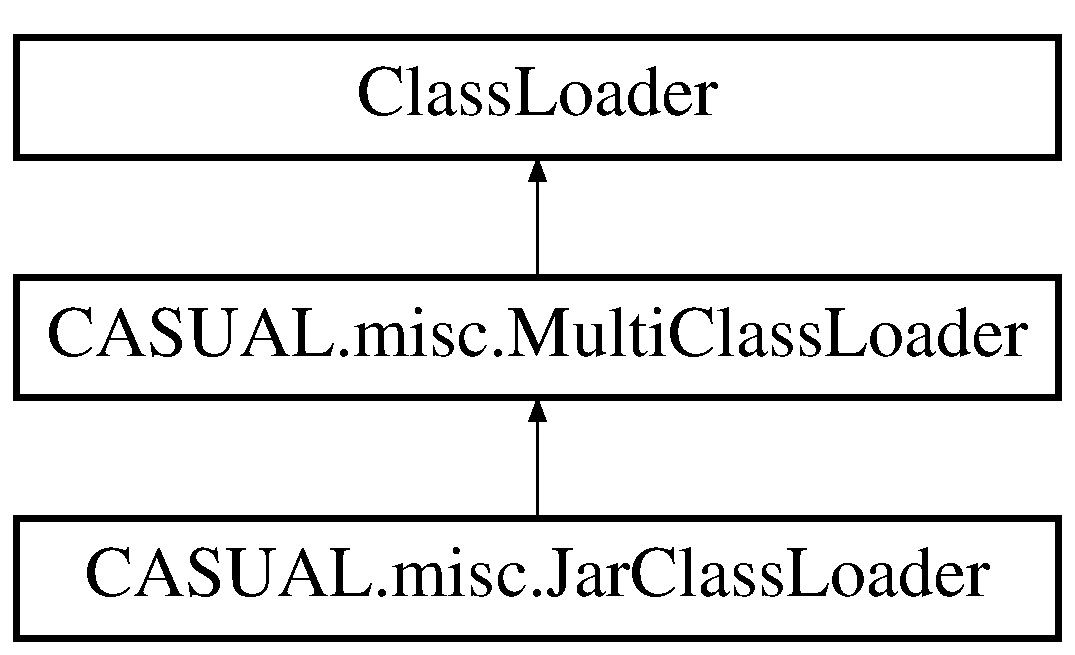
\includegraphics[height=3.000000cm]{classCASUAL_1_1misc_1_1JarClassLoader}
\end{center}
\end{figure}
\subsection*{Public Member Functions}
\begin{DoxyCompactItemize}
\item 
\hypertarget{classCASUAL_1_1misc_1_1JarClassLoader_abe0e288f93e15f027d42ee33ae2c029b}{{\bfseries Jar\-Class\-Loader} (String jar\-Name)}\label{classCASUAL_1_1misc_1_1JarClassLoader_abe0e288f93e15f027d42ee33ae2c029b}

\end{DoxyCompactItemize}
\subsection*{Protected Member Functions}
\begin{DoxyCompactItemize}
\item 
\hypertarget{classCASUAL_1_1misc_1_1JarClassLoader_a7ddea315a610ec4cdaadea99d4c91801}{byte\mbox{[}$\,$\mbox{]} {\bfseries load\-Class\-Bytes} (String class\-Name)}\label{classCASUAL_1_1misc_1_1JarClassLoader_a7ddea315a610ec4cdaadea99d4c91801}

\end{DoxyCompactItemize}
\subsection*{Additional Inherited Members}


The documentation for this class was generated from the following file\-:\begin{DoxyCompactItemize}
\item 
trunk/\-C\-A\-S\-U\-A\-Lcore/test/\-C\-A\-S\-U\-A\-L/misc/Jar\-Class\-Loader.\-java\end{DoxyCompactItemize}

\hypertarget{classCASUAL_1_1misc_1_1JarResources}{\section{C\-A\-S\-U\-A\-L.\-misc.\-Jar\-Resources Class Reference}
\label{classCASUAL_1_1misc_1_1JarResources}\index{C\-A\-S\-U\-A\-L.\-misc.\-Jar\-Resources@{C\-A\-S\-U\-A\-L.\-misc.\-Jar\-Resources}}
}
\subsection*{Public Member Functions}
\begin{DoxyCompactItemize}
\item 
\hyperlink{classCASUAL_1_1misc_1_1JarResources_ac8ba46fea06a1252e082af6ea9a839e0}{Jar\-Resources} (String jar\-File\-Name)
\item 
byte\mbox{[}$\,$\mbox{]} \hyperlink{classCASUAL_1_1misc_1_1JarResources_a85bd36fff3d70021db81964e513872e3}{get\-Resource} (String name)
\end{DoxyCompactItemize}
\subsection*{Static Public Member Functions}
\begin{DoxyCompactItemize}
\item 
static void \hyperlink{classCASUAL_1_1misc_1_1JarResources_a63053fd99282d4d90035563a5e2a5aa1}{main} (String\mbox{[}$\,$\mbox{]} args)  throws I\-O\-Exception 
\end{DoxyCompactItemize}
\subsection*{Public Attributes}
\begin{DoxyCompactItemize}
\item 
\hypertarget{classCASUAL_1_1misc_1_1JarResources_a4b866bc0269cf9342e439ebbb5babf43}{boolean {\bfseries debug\-On} = false}\label{classCASUAL_1_1misc_1_1JarResources_a4b866bc0269cf9342e439ebbb5babf43}

\end{DoxyCompactItemize}


\subsection{Detailed Description}
\hyperlink{classCASUAL_1_1misc_1_1JarResources}{Jar\-Resources}\-: \hyperlink{classCASUAL_1_1misc_1_1JarResources}{Jar\-Resources} maps all resources included in a Zip or Jar file. Additionaly, it provides a method to extract one as a blob. 

\subsection{Constructor \& Destructor Documentation}
\hypertarget{classCASUAL_1_1misc_1_1JarResources_ac8ba46fea06a1252e082af6ea9a839e0}{\index{C\-A\-S\-U\-A\-L\-::misc\-::\-Jar\-Resources@{C\-A\-S\-U\-A\-L\-::misc\-::\-Jar\-Resources}!Jar\-Resources@{Jar\-Resources}}
\index{Jar\-Resources@{Jar\-Resources}!CASUAL::misc::JarResources@{C\-A\-S\-U\-A\-L\-::misc\-::\-Jar\-Resources}}
\subsubsection[{Jar\-Resources}]{\setlength{\rightskip}{0pt plus 5cm}C\-A\-S\-U\-A\-L.\-misc.\-Jar\-Resources.\-Jar\-Resources (
\begin{DoxyParamCaption}
\item[{String}]{jar\-File\-Name}
\end{DoxyParamCaption}
)}}\label{classCASUAL_1_1misc_1_1JarResources_ac8ba46fea06a1252e082af6ea9a839e0}
creates a \hyperlink{classCASUAL_1_1misc_1_1JarResources}{Jar\-Resources}. It extracts all resources from a Jar into an internal hashtable, keyed by resource names.


\begin{DoxyParams}{Parameters}
{\em jar\-File\-Name} & a jar or zip file \\
\hline
\end{DoxyParams}


\subsection{Member Function Documentation}
\hypertarget{classCASUAL_1_1misc_1_1JarResources_a85bd36fff3d70021db81964e513872e3}{\index{C\-A\-S\-U\-A\-L\-::misc\-::\-Jar\-Resources@{C\-A\-S\-U\-A\-L\-::misc\-::\-Jar\-Resources}!get\-Resource@{get\-Resource}}
\index{get\-Resource@{get\-Resource}!CASUAL::misc::JarResources@{C\-A\-S\-U\-A\-L\-::misc\-::\-Jar\-Resources}}
\subsubsection[{get\-Resource}]{\setlength{\rightskip}{0pt plus 5cm}byte \mbox{[}$\,$\mbox{]} C\-A\-S\-U\-A\-L.\-misc.\-Jar\-Resources.\-get\-Resource (
\begin{DoxyParamCaption}
\item[{String}]{name}
\end{DoxyParamCaption}
)}}\label{classCASUAL_1_1misc_1_1JarResources_a85bd36fff3d70021db81964e513872e3}
Extracts a jar resource as a blob.


\begin{DoxyParams}{Parameters}
{\em name} & a resource name. \\
\hline
\end{DoxyParams}
\hypertarget{classCASUAL_1_1misc_1_1JarResources_a63053fd99282d4d90035563a5e2a5aa1}{\index{C\-A\-S\-U\-A\-L\-::misc\-::\-Jar\-Resources@{C\-A\-S\-U\-A\-L\-::misc\-::\-Jar\-Resources}!main@{main}}
\index{main@{main}!CASUAL::misc::JarResources@{C\-A\-S\-U\-A\-L\-::misc\-::\-Jar\-Resources}}
\subsubsection[{main}]{\setlength{\rightskip}{0pt plus 5cm}static void C\-A\-S\-U\-A\-L.\-misc.\-Jar\-Resources.\-main (
\begin{DoxyParamCaption}
\item[{String\mbox{[}$\,$\mbox{]}}]{args}
\end{DoxyParamCaption}
) throws I\-O\-Exception\hspace{0.3cm}{\ttfamily [static]}}}\label{classCASUAL_1_1misc_1_1JarResources_a63053fd99282d4d90035563a5e2a5aa1}
Is a test driver. Given a jar file and a resource name, it trys to extract the resource and then tells us whether it could or not.

{\bfseries Example} Let's say you have a J\-A\-R file which jarred up a bunch of gif image files. Now, by using \hyperlink{classCASUAL_1_1misc_1_1JarResources}{Jar\-Resources}, you could extract, create, and display those images on-\/the-\/fly. 
\begin{DoxyPre}
    ...
    \hyperlink{classCASUAL_1_1misc_1_1JarResources}{JarResources} JR=new \hyperlink{classCASUAL_1_1misc_1_1JarResources}{JarResources}("GifBundle.jar");
    Image image=Toolkit.createImage(JR.getResource("logo.gif");
    Image logo=Toolkit.getDefaultToolkit().createImage(
                  JR.getResources("logo.gif")
                  );
    ...
\end{DoxyPre}
 

The documentation for this class was generated from the following file\-:\begin{DoxyCompactItemize}
\item 
trunk/\-C\-A\-S\-U\-A\-Lcore/test/\-C\-A\-S\-U\-A\-L/misc/Jar\-Resources.\-java\end{DoxyCompactItemize}

\hypertarget{classCASUAL_1_1JavaSystem}{\section{C\-A\-S\-U\-A\-L.\-Java\-System Class Reference}
\label{classCASUAL_1_1JavaSystem}\index{C\-A\-S\-U\-A\-L.\-Java\-System@{C\-A\-S\-U\-A\-L.\-Java\-System}}
}
\subsection*{Static Public Member Functions}
\begin{DoxyCompactItemize}
\item 
static void \hyperlink{classCASUAL_1_1JavaSystem_a536b49d9c60a616ee7410b665842c967}{restart} (String\mbox{[}$\,$\mbox{]} args)  throws I\-O\-Exception, Interrupted\-Exception 
\item 
\hypertarget{classCASUAL_1_1JavaSystem_a6b77ae0dc01d8e5208e65c06784e6da9}{static void {\bfseries launch} (String\mbox{[}$\,$\mbox{]} args)  throws I\-O\-Exception, Interrupted\-Exception }\label{classCASUAL_1_1JavaSystem_a6b77ae0dc01d8e5208e65c06784e6da9}

\end{DoxyCompactItemize}


\subsection{Detailed Description}
\begin{DoxyAuthor}{Author}
adam 
\end{DoxyAuthor}


\subsection{Member Function Documentation}
\hypertarget{classCASUAL_1_1JavaSystem_a536b49d9c60a616ee7410b665842c967}{\index{C\-A\-S\-U\-A\-L\-::\-Java\-System@{C\-A\-S\-U\-A\-L\-::\-Java\-System}!restart@{restart}}
\index{restart@{restart}!CASUAL::JavaSystem@{C\-A\-S\-U\-A\-L\-::\-Java\-System}}
\subsubsection[{restart}]{\setlength{\rightskip}{0pt plus 5cm}static void C\-A\-S\-U\-A\-L.\-Java\-System.\-restart (
\begin{DoxyParamCaption}
\item[{String\mbox{[}$\,$\mbox{]}}]{args}
\end{DoxyParamCaption}
) throws I\-O\-Exception, Interrupted\-Exception\hspace{0.3cm}{\ttfamily [static]}}}\label{classCASUAL_1_1JavaSystem_a536b49d9c60a616ee7410b665842c967}
restarts java


\begin{DoxyParams}{Parameters}
{\em args} & args to add \\
\hline
\end{DoxyParams}

\begin{DoxyExceptions}{Exceptions}
{\em I\-O\-Exception} & \\
\hline
{\em Interrupted\-Exception} & \\
\hline
\end{DoxyExceptions}


The documentation for this class was generated from the following file\-:\begin{DoxyCompactItemize}
\item 
trunk/\-C\-A\-S\-U\-A\-Lcore/src/\-C\-A\-S\-U\-A\-L/Java\-System.\-java\end{DoxyCompactItemize}

\hypertarget{classCASUAL_1_1misc_1_1LinkedProperties}{\section{C\-A\-S\-U\-A\-L.\-misc.\-Linked\-Properties Class Reference}
\label{classCASUAL_1_1misc_1_1LinkedProperties}\index{C\-A\-S\-U\-A\-L.\-misc.\-Linked\-Properties@{C\-A\-S\-U\-A\-L.\-misc.\-Linked\-Properties}}
}
Inheritance diagram for C\-A\-S\-U\-A\-L.\-misc.\-Linked\-Properties\-:\begin{figure}[H]
\begin{center}
\leavevmode
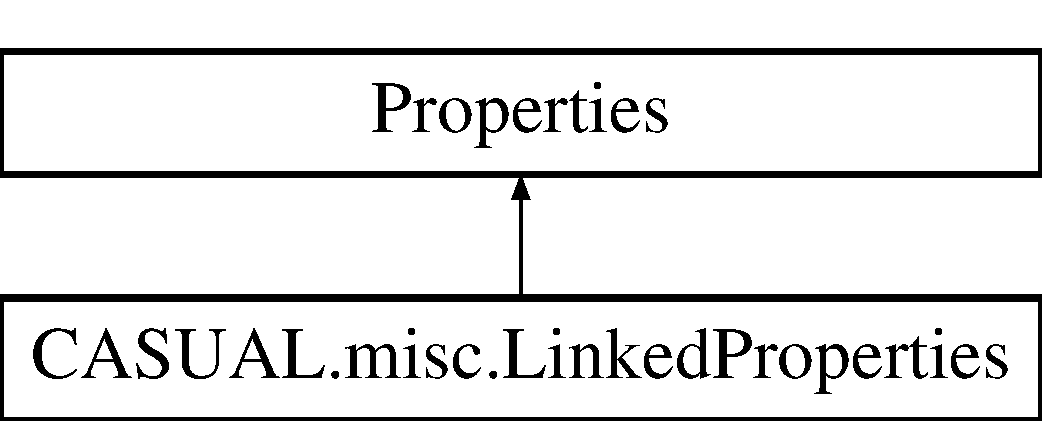
\includegraphics[height=2.000000cm]{classCASUAL_1_1misc_1_1LinkedProperties}
\end{center}
\end{figure}
\subsection*{Public Member Functions}
\begin{DoxyCompactItemize}
\item 
Enumeration$<$ Object $>$ \hyperlink{classCASUAL_1_1misc_1_1LinkedProperties_a70ea068b7aef6f29a3221e6de67f962f}{keys} ()
\item 
Object \hyperlink{classCASUAL_1_1misc_1_1LinkedProperties_a56ef8e557095be6869bf1c4562cd6deb}{put} (Object key, Object value)
\item 
Set$<$ String $>$ \hyperlink{classCASUAL_1_1misc_1_1LinkedProperties_a2bc321d6ef4204f9d01b26fae22ae510}{string\-Property\-Names} ()
\end{DoxyCompactItemize}


\subsection{Detailed Description}
\hyperlink{classCASUAL_1_1misc_1_1LinkedProperties}{Linked\-Properties} allows for a static order to be placed on a properties file rather than random/last-\/modified order generally used in writing a properties file. \begin{DoxyAuthor}{Author}
Adam Outler \href{mailto:adamoutler@gmail.com}{\tt adamoutler@gmail.\-com} inspired\-By \href{http://stackoverflow.com/questions/1312383/pulling-values-from-a-java-properties-file-in-order}{\tt http\-://stackoverflow.\-com/questions/1312383/pulling-\/values-\/from-\/a-\/java-\/properties-\/file-\/in-\/order} 
\end{DoxyAuthor}


\subsection{Member Function Documentation}
\hypertarget{classCASUAL_1_1misc_1_1LinkedProperties_a70ea068b7aef6f29a3221e6de67f962f}{\index{C\-A\-S\-U\-A\-L\-::misc\-::\-Linked\-Properties@{C\-A\-S\-U\-A\-L\-::misc\-::\-Linked\-Properties}!keys@{keys}}
\index{keys@{keys}!CASUAL::misc::LinkedProperties@{C\-A\-S\-U\-A\-L\-::misc\-::\-Linked\-Properties}}
\subsubsection[{keys}]{\setlength{\rightskip}{0pt plus 5cm}Enumeration$<$Object$>$ C\-A\-S\-U\-A\-L.\-misc.\-Linked\-Properties.\-keys (
\begin{DoxyParamCaption}
{}
\end{DoxyParamCaption}
)}}\label{classCASUAL_1_1misc_1_1LinkedProperties_a70ea068b7aef6f29a3221e6de67f962f}
gets the keys in the properties list \begin{DoxyReturn}{Returns}
all the keys in the properties list 
\end{DoxyReturn}
\hypertarget{classCASUAL_1_1misc_1_1LinkedProperties_a56ef8e557095be6869bf1c4562cd6deb}{\index{C\-A\-S\-U\-A\-L\-::misc\-::\-Linked\-Properties@{C\-A\-S\-U\-A\-L\-::misc\-::\-Linked\-Properties}!put@{put}}
\index{put@{put}!CASUAL::misc::LinkedProperties@{C\-A\-S\-U\-A\-L\-::misc\-::\-Linked\-Properties}}
\subsubsection[{put}]{\setlength{\rightskip}{0pt plus 5cm}Object C\-A\-S\-U\-A\-L.\-misc.\-Linked\-Properties.\-put (
\begin{DoxyParamCaption}
\item[{Object}]{key, }
\item[{Object}]{value}
\end{DoxyParamCaption}
)}}\label{classCASUAL_1_1misc_1_1LinkedProperties_a56ef8e557095be6869bf1c4562cd6deb}
puts a value into the properties list 
\begin{DoxyParams}{Parameters}
{\em key} & \\
\hline
{\em value} & \\
\hline
\end{DoxyParams}
\begin{DoxyReturn}{Returns}

\end{DoxyReturn}
\hypertarget{classCASUAL_1_1misc_1_1LinkedProperties_a2bc321d6ef4204f9d01b26fae22ae510}{\index{C\-A\-S\-U\-A\-L\-::misc\-::\-Linked\-Properties@{C\-A\-S\-U\-A\-L\-::misc\-::\-Linked\-Properties}!string\-Property\-Names@{string\-Property\-Names}}
\index{string\-Property\-Names@{string\-Property\-Names}!CASUAL::misc::LinkedProperties@{C\-A\-S\-U\-A\-L\-::misc\-::\-Linked\-Properties}}
\subsubsection[{string\-Property\-Names}]{\setlength{\rightskip}{0pt plus 5cm}Set$<$String$>$ C\-A\-S\-U\-A\-L.\-misc.\-Linked\-Properties.\-string\-Property\-Names (
\begin{DoxyParamCaption}
{}
\end{DoxyParamCaption}
)}}\label{classCASUAL_1_1misc_1_1LinkedProperties_a2bc321d6ef4204f9d01b26fae22ae510}
gets names of the properties in the list \begin{DoxyReturn}{Returns}
set of propertiy names 
\end{DoxyReturn}


The documentation for this class was generated from the following file\-:\begin{DoxyCompactItemize}
\item 
trunk/\-C\-A\-S\-U\-A\-Lcore/src/\-C\-A\-S\-U\-A\-L/misc/Linked\-Properties.\-java\end{DoxyCompactItemize}

\hypertarget{classCASUAL_1_1network_1_1LinkLauncher}{\section{C\-A\-S\-U\-A\-L.\-network.\-Link\-Launcher Class Reference}
\label{classCASUAL_1_1network_1_1LinkLauncher}\index{C\-A\-S\-U\-A\-L.\-network.\-Link\-Launcher@{C\-A\-S\-U\-A\-L.\-network.\-Link\-Launcher}}
}
\subsection*{Public Member Functions}
\begin{DoxyCompactItemize}
\item 
\hyperlink{classCASUAL_1_1network_1_1LinkLauncher_abd6e04f6aa0db90be661585188fb88fd}{Link\-Launcher} (String link)
\item 
void \hyperlink{classCASUAL_1_1network_1_1LinkLauncher_adfb4c64904f505f11ff130d83f659339}{launch} ()
\end{DoxyCompactItemize}


\subsection{Detailed Description}
\begin{DoxyAuthor}{Author}
adam 
\end{DoxyAuthor}


\subsection{Constructor \& Destructor Documentation}
\hypertarget{classCASUAL_1_1network_1_1LinkLauncher_abd6e04f6aa0db90be661585188fb88fd}{\index{C\-A\-S\-U\-A\-L\-::network\-::\-Link\-Launcher@{C\-A\-S\-U\-A\-L\-::network\-::\-Link\-Launcher}!Link\-Launcher@{Link\-Launcher}}
\index{Link\-Launcher@{Link\-Launcher}!CASUAL::network::LinkLauncher@{C\-A\-S\-U\-A\-L\-::network\-::\-Link\-Launcher}}
\subsubsection[{Link\-Launcher}]{\setlength{\rightskip}{0pt plus 5cm}C\-A\-S\-U\-A\-L.\-network.\-Link\-Launcher.\-Link\-Launcher (
\begin{DoxyParamCaption}
\item[{String}]{link}
\end{DoxyParamCaption}
)}}\label{classCASUAL_1_1network_1_1LinkLauncher_abd6e04f6aa0db90be661585188fb88fd}
launches a browser with a link


\begin{DoxyParams}{Parameters}
{\em link} & link to launch \\
\hline
\end{DoxyParams}


\subsection{Member Function Documentation}
\hypertarget{classCASUAL_1_1network_1_1LinkLauncher_adfb4c64904f505f11ff130d83f659339}{\index{C\-A\-S\-U\-A\-L\-::network\-::\-Link\-Launcher@{C\-A\-S\-U\-A\-L\-::network\-::\-Link\-Launcher}!launch@{launch}}
\index{launch@{launch}!CASUAL::network::LinkLauncher@{C\-A\-S\-U\-A\-L\-::network\-::\-Link\-Launcher}}
\subsubsection[{launch}]{\setlength{\rightskip}{0pt plus 5cm}void C\-A\-S\-U\-A\-L.\-network.\-Link\-Launcher.\-launch (
\begin{DoxyParamCaption}
{}
\end{DoxyParamCaption}
)}}\label{classCASUAL_1_1network_1_1LinkLauncher_adfb4c64904f505f11ff130d83f659339}
launches the link commanded in constructor 

The documentation for this class was generated from the following file\-:\begin{DoxyCompactItemize}
\item 
trunk/\-C\-A\-S\-U\-A\-Lcore/src/\-C\-A\-S\-U\-A\-L/network/Link\-Launcher.\-java\end{DoxyCompactItemize}

\hypertarget{classCASUAL_1_1LinkLauncher}{\section{C\-A\-S\-U\-A\-L.\-Link\-Launcher Class Reference}
\label{classCASUAL_1_1LinkLauncher}\index{C\-A\-S\-U\-A\-L.\-Link\-Launcher@{C\-A\-S\-U\-A\-L.\-Link\-Launcher}}
}
Inheritance diagram for C\-A\-S\-U\-A\-L.\-Link\-Launcher\-:\begin{figure}[H]
\begin{center}
\leavevmode
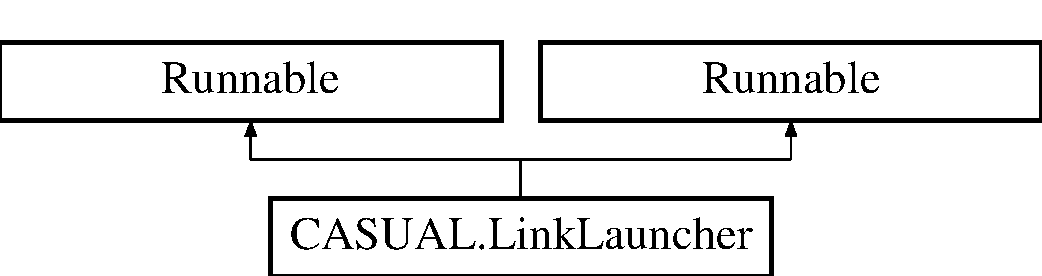
\includegraphics[height=2.000000cm]{classCASUAL_1_1LinkLauncher}
\end{center}
\end{figure}
\subsection*{Public Member Functions}
\begin{DoxyCompactItemize}
\item 
\hypertarget{classCASUAL_1_1LinkLauncher_a857267bfe6dd77a071c3292fd844928b}{void {\bfseries launch\-Link} (String link)}\label{classCASUAL_1_1LinkLauncher_a857267bfe6dd77a071c3292fd844928b}

\item 
\hypertarget{classCASUAL_1_1LinkLauncher_a6b88e74888a1ea9dc4e5a4c439ae97a0}{void {\bfseries run} ()}\label{classCASUAL_1_1LinkLauncher_a6b88e74888a1ea9dc4e5a4c439ae97a0}

\item 
\hypertarget{classCASUAL_1_1LinkLauncher_a857267bfe6dd77a071c3292fd844928b}{void {\bfseries launch\-Link} (String link)}\label{classCASUAL_1_1LinkLauncher_a857267bfe6dd77a071c3292fd844928b}

\item 
\hypertarget{classCASUAL_1_1LinkLauncher_a6b88e74888a1ea9dc4e5a4c439ae97a0}{void {\bfseries run} ()}\label{classCASUAL_1_1LinkLauncher_a6b88e74888a1ea9dc4e5a4c439ae97a0}

\end{DoxyCompactItemize}


\subsection{Detailed Description}
\begin{DoxyAuthor}{Author}
adam 
\end{DoxyAuthor}


The documentation for this class was generated from the following files\-:\begin{DoxyCompactItemize}
\item 
branches/\-C\-A\-S\-U\-A\-L-\/\-Headless/\-G\-U\-I/src/\-C\-A\-S\-U\-A\-L/Link\-Launcher.\-java\item 
branches/\-Testing\-Branch/\-G\-Doc/src/\-C\-A\-S\-U\-A\-L/Link\-Launcher.\-java\end{DoxyCompactItemize}

\hypertarget{classCASUAL_1_1Locks}{\section{C\-A\-S\-U\-A\-L.\-Locks Class Reference}
\label{classCASUAL_1_1Locks}\index{C\-A\-S\-U\-A\-L.\-Locks@{C\-A\-S\-U\-A\-L.\-Locks}}
}
\subsection*{Static Public Attributes}
\begin{DoxyCompactItemize}
\item 
static Thread {\bfseries start\-G\-U\-I}
\item 
\hypertarget{classCASUAL_1_1Locks_a4c5cfed071b9314a781143939b6ca59f}{static \hyperlink{classCASUAL_1_1misc_1_1MandatoryThread}{Mandatory\-Thread} {\bfseries script\-Run\-Lock} =new \hyperlink{classCASUAL_1_1misc_1_1MandatoryThread}{Mandatory\-Thread}()}\label{classCASUAL_1_1Locks_a4c5cfed071b9314a781143939b6ca59f}

\item 
\hypertarget{classCASUAL_1_1Locks_a58d1360da878b0d7707313703e7edbf9}{static boolean {\bfseries lock\-G\-U\-Iform\-Prep} = true}\label{classCASUAL_1_1Locks_a58d1360da878b0d7707313703e7edbf9}

\item 
\hypertarget{classCASUAL_1_1Locks_a51d3cb2cd6ddb238ada918a75ef3dcc8}{static boolean {\bfseries lock\-G\-U\-Iunzip} = true}\label{classCASUAL_1_1Locks_a51d3cb2cd6ddb238ada918a75ef3dcc8}

\item 
\hypertarget{classCASUAL_1_1Locks_ac79b2141772d3690d9fe2ad8b8a8a649}{static boolean {\bfseries caspac\-Script\-Prep\-Lock} = true}\label{classCASUAL_1_1Locks_ac79b2141772d3690d9fe2ad8b8a8a649}

\end{DoxyCompactItemize}


\subsection{Detailed Description}
\begin{DoxyAuthor}{Author}
adamoutler 
\end{DoxyAuthor}


\subsection{Member Data Documentation}
\hypertarget{classCASUAL_1_1Locks_aab99d065f2c885eeb6ec25a5253c67fd}{\index{C\-A\-S\-U\-A\-L\-::\-Locks@{C\-A\-S\-U\-A\-L\-::\-Locks}!start\-G\-U\-I@{start\-G\-U\-I}}
\index{start\-G\-U\-I@{start\-G\-U\-I}!CASUAL::Locks@{C\-A\-S\-U\-A\-L\-::\-Locks}}
\subsubsection[{start\-G\-U\-I}]{\setlength{\rightskip}{0pt plus 5cm}Thread C\-A\-S\-U\-A\-L.\-Locks.\-start\-G\-U\-I\hspace{0.3cm}{\ttfamily [static]}}}\label{classCASUAL_1_1Locks_aab99d065f2c885eeb6ec25a5253c67fd}
{\bfseries Initial value\-:}
\begin{DoxyCode}
= \textcolor{keyword}{new} Thread(\textcolor{keyword}{new} Runnable() \{

        @Override
        \textcolor{keyword}{public} \textcolor{keywordtype}{void} run() \{
            \textcolor{keywordflow}{if} (CASUALMain.useGUI || Statics.dumbTerminalGUI) \{
                startGUI = \textcolor{keyword}{new} Thread(\textcolor{keyword}{new} CASUALTools().GUI);
                startGUI.setName(\textcolor{stringliteral}{"CASUAL GUI"});
                Statics.setStatus(\textcolor{stringliteral}{"launching GUI"});
                startGUI.start();
            \}
        \}

    \})
\end{DoxyCode}


The documentation for this class was generated from the following file\-:\begin{DoxyCompactItemize}
\item 
trunk/\-C\-A\-S\-U\-A\-Lcore/src/\-C\-A\-S\-U\-A\-L/Locks.\-java\end{DoxyCompactItemize}

\hypertarget{classCASUAL_1_1Log}{\section{C\-A\-S\-U\-A\-L.\-Log Class Reference}
\label{classCASUAL_1_1Log}\index{C\-A\-S\-U\-A\-L.\-Log@{C\-A\-S\-U\-A\-L.\-Log}}
}
\subsection*{Public Member Functions}
\begin{DoxyCompactItemize}
\item 
\hypertarget{classCASUAL_1_1Log_af6e3bfc98540f4b2b4a7b8f0972ff46b}{void {\bfseries level0} (String data)}\label{classCASUAL_1_1Log_af6e3bfc98540f4b2b4a7b8f0972ff46b}

\item 
\hypertarget{classCASUAL_1_1Log_ae15ba5a18f0da5ffb5ec23cbc9e27bb7}{void {\bfseries level1} (String data)}\label{classCASUAL_1_1Log_ae15ba5a18f0da5ffb5ec23cbc9e27bb7}

\item 
\hypertarget{classCASUAL_1_1Log_ae587e45a337671bec97c3dd12296e6d6}{void {\bfseries level2} (String data)}\label{classCASUAL_1_1Log_ae587e45a337671bec97c3dd12296e6d6}

\item 
\hypertarget{classCASUAL_1_1Log_a24fad4a3a0a91ef33054eb9c04133963}{void {\bfseries level3} (String data)}\label{classCASUAL_1_1Log_a24fad4a3a0a91ef33054eb9c04133963}

\item 
\hypertarget{classCASUAL_1_1Log_aa20b5a7ed3c68f65559b127a2c14231f}{void {\bfseries copy\-Error} (String Filename)}\label{classCASUAL_1_1Log_aa20b5a7ed3c68f65559b127a2c14231f}

\item 
\hypertarget{classCASUAL_1_1Log_ad87445d4bff7a19de8b254e795ee5dc2}{void {\bfseries generic\-Error} (String Message)}\label{classCASUAL_1_1Log_ad87445d4bff7a19de8b254e795ee5dc2}

\item 
\hypertarget{classCASUAL_1_1Log_acd0cd0a6ea0d89511fd97317715daa72}{void {\bfseries write\-To\-Log\-File} (String data)}\label{classCASUAL_1_1Log_acd0cd0a6ea0d89511fd97317715daa72}

\item 
\hypertarget{classCASUAL_1_1Log_ac7992ba5f3159c62058e5477c2ad4f5c}{void {\bfseries progress} (String data)}\label{classCASUAL_1_1Log_ac7992ba5f3159c62058e5477c2ad4f5c}

\item 
\hypertarget{classCASUAL_1_1Log_a5d1038ccb55197df55664c7b62adc810}{void {\bfseries Live\-Update} (String data)}\label{classCASUAL_1_1Log_a5d1038ccb55197df55664c7b62adc810}

\item 
\hypertarget{classCASUAL_1_1Log_a1d6df28a1115d39b98d7d4f205d3e071}{void {\bfseries begin\-Line} ()}\label{classCASUAL_1_1Log_a1d6df28a1115d39b98d7d4f205d3e071}

\item 
\hypertarget{classCASUAL_1_1Log_af6e3bfc98540f4b2b4a7b8f0972ff46b}{void {\bfseries level0} (String data)}\label{classCASUAL_1_1Log_af6e3bfc98540f4b2b4a7b8f0972ff46b}

\item 
\hypertarget{classCASUAL_1_1Log_ae15ba5a18f0da5ffb5ec23cbc9e27bb7}{void {\bfseries level1} (String data)}\label{classCASUAL_1_1Log_ae15ba5a18f0da5ffb5ec23cbc9e27bb7}

\item 
\hypertarget{classCASUAL_1_1Log_ae587e45a337671bec97c3dd12296e6d6}{void {\bfseries level2} (String data)}\label{classCASUAL_1_1Log_ae587e45a337671bec97c3dd12296e6d6}

\item 
\hypertarget{classCASUAL_1_1Log_a24fad4a3a0a91ef33054eb9c04133963}{void {\bfseries level3} (String data)}\label{classCASUAL_1_1Log_a24fad4a3a0a91ef33054eb9c04133963}

\item 
\hypertarget{classCASUAL_1_1Log_aa20b5a7ed3c68f65559b127a2c14231f}{void {\bfseries copy\-Error} (String Filename)}\label{classCASUAL_1_1Log_aa20b5a7ed3c68f65559b127a2c14231f}

\item 
\hypertarget{classCASUAL_1_1Log_ad87445d4bff7a19de8b254e795ee5dc2}{void {\bfseries generic\-Error} (String Message)}\label{classCASUAL_1_1Log_ad87445d4bff7a19de8b254e795ee5dc2}

\item 
\hypertarget{classCASUAL_1_1Log_acd0cd0a6ea0d89511fd97317715daa72}{void {\bfseries write\-To\-Log\-File} (String data)}\label{classCASUAL_1_1Log_acd0cd0a6ea0d89511fd97317715daa72}

\item 
\hypertarget{classCASUAL_1_1Log_ac7992ba5f3159c62058e5477c2ad4f5c}{void {\bfseries progress} (String data)}\label{classCASUAL_1_1Log_ac7992ba5f3159c62058e5477c2ad4f5c}

\item 
\hypertarget{classCASUAL_1_1Log_a5d1038ccb55197df55664c7b62adc810}{void {\bfseries Live\-Update} (String data)}\label{classCASUAL_1_1Log_a5d1038ccb55197df55664c7b62adc810}

\item 
\hypertarget{classCASUAL_1_1Log_a1d6df28a1115d39b98d7d4f205d3e071}{void {\bfseries begin\-Line} ()}\label{classCASUAL_1_1Log_a1d6df28a1115d39b98d7d4f205d3e071}

\item 
\hypertarget{classCASUAL_1_1Log_ab95e98c154362d8c538a9d056004581c}{void {\bfseries clear\-G\-U\-I} ()}\label{classCASUAL_1_1Log_ab95e98c154362d8c538a9d056004581c}

\item 
void \hyperlink{classCASUAL_1_1Log_afc35f2858108aa81be706cd2d6677ed2}{level0\-Error} (String data)
\item 
void \hyperlink{classCASUAL_1_1Log_a06abaf9f5e1511bdd79a2b9cebd9b4a0}{Level1\-Interaction} (String data)
\item 
void \hyperlink{classCASUAL_1_1Log_aa414ecc1573182ea68c55c9be1f4870a}{level2\-Information} (String data)
\item 
void \hyperlink{classCASUAL_1_1Log_a2ddc8d9b645b62e1ceb3037e24670190}{level3\-Verbose} (String data)
\item 
void \hyperlink{classCASUAL_1_1Log_ab674594609b46c9e6657818be10d1789}{level4\-Debug} (String data)
\item 
void \hyperlink{classCASUAL_1_1Log_acd0cd0a6ea0d89511fd97317715daa72}{write\-To\-Log\-File} (String data)
\item 
void \hyperlink{classCASUAL_1_1Log_ac7992ba5f3159c62058e5477c2ad4f5c}{progress} (String data)
\item 
void \hyperlink{classCASUAL_1_1Log_a5d1038ccb55197df55664c7b62adc810}{Live\-Update} (String data)
\item 
void \hyperlink{classCASUAL_1_1Log_a1d6df28a1115d39b98d7d4f205d3e071}{begin\-Line} ()
\item 
\hypertarget{classCASUAL_1_1Log_a46852a574166ce1c0f1d20b5f4122363}{void {\bfseries replace\-Line} (String data, int position, int length)}\label{classCASUAL_1_1Log_a46852a574166ce1c0f1d20b5f4122363}

\item 
void \hyperlink{classCASUAL_1_1Log_a90ec16385f2b20b9f06e367c22f34af2}{error\-Handler} (Exception e)
\end{DoxyCompactItemize}
\subsection*{Static Public Attributes}
\begin{DoxyCompactItemize}
\item 
static Print\-Stream \hyperlink{classCASUAL_1_1Log_a004327eeb7230d6af9f995b257a656ff}{out} = new Print\-Stream(System.\-out)
\end{DoxyCompactItemize}


\subsection{Detailed Description}
\begin{DoxyAuthor}{Author}
adam Logging levels\-: Logging levels are set in \hyperlink{classCASUAL_1_1Statics}{Statics}
\end{DoxyAuthor}
Level0\-: silent, keep this for future critical tasks Level1\-: Information for user to see Level2\-: Information for developers to see Level3\-: verbose information, use for conversions and random tasks 

\subsection{Member Function Documentation}
\hypertarget{classCASUAL_1_1Log_a1d6df28a1115d39b98d7d4f205d3e071}{\index{C\-A\-S\-U\-A\-L\-::\-Log@{C\-A\-S\-U\-A\-L\-::\-Log}!begin\-Line@{begin\-Line}}
\index{begin\-Line@{begin\-Line}!CASUAL::Log@{C\-A\-S\-U\-A\-L\-::\-Log}}
\subsubsection[{begin\-Line}]{\setlength{\rightskip}{0pt plus 5cm}void C\-A\-S\-U\-A\-L.\-Log.\-begin\-Line (
\begin{DoxyParamCaption}
{}
\end{DoxyParamCaption}
)}}\label{classCASUAL_1_1Log_a1d6df28a1115d39b98d7d4f205d3e071}
begins a new line \hypertarget{classCASUAL_1_1Log_a90ec16385f2b20b9f06e367c22f34af2}{\index{C\-A\-S\-U\-A\-L\-::\-Log@{C\-A\-S\-U\-A\-L\-::\-Log}!error\-Handler@{error\-Handler}}
\index{error\-Handler@{error\-Handler}!CASUAL::Log@{C\-A\-S\-U\-A\-L\-::\-Log}}
\subsubsection[{error\-Handler}]{\setlength{\rightskip}{0pt plus 5cm}void C\-A\-S\-U\-A\-L.\-Log.\-error\-Handler (
\begin{DoxyParamCaption}
\item[{Exception}]{e}
\end{DoxyParamCaption}
)}}\label{classCASUAL_1_1Log_a90ec16385f2b20b9f06e367c22f34af2}

\begin{DoxyParams}{Parameters}
{\em e} & is any Throwable. \\
\hline
\end{DoxyParams}
\hypertarget{classCASUAL_1_1Log_afc35f2858108aa81be706cd2d6677ed2}{\index{C\-A\-S\-U\-A\-L\-::\-Log@{C\-A\-S\-U\-A\-L\-::\-Log}!level0\-Error@{level0\-Error}}
\index{level0\-Error@{level0\-Error}!CASUAL::Log@{C\-A\-S\-U\-A\-L\-::\-Log}}
\subsubsection[{level0\-Error}]{\setlength{\rightskip}{0pt plus 5cm}void C\-A\-S\-U\-A\-L.\-Log.\-level0\-Error (
\begin{DoxyParamCaption}
\item[{String}]{data}
\end{DoxyParamCaption}
)}}\label{classCASUAL_1_1Log_afc35f2858108aa81be706cd2d6677ed2}
level 0 is used for errors.. basically silent. Use level 1 for for most tasks


\begin{DoxyParams}{Parameters}
{\em data} & is data to be written to log \\
\hline
\end{DoxyParams}
\hypertarget{classCASUAL_1_1Log_a06abaf9f5e1511bdd79a2b9cebd9b4a0}{\index{C\-A\-S\-U\-A\-L\-::\-Log@{C\-A\-S\-U\-A\-L\-::\-Log}!Level1\-Interaction@{Level1\-Interaction}}
\index{Level1\-Interaction@{Level1\-Interaction}!CASUAL::Log@{C\-A\-S\-U\-A\-L\-::\-Log}}
\subsubsection[{Level1\-Interaction}]{\setlength{\rightskip}{0pt plus 5cm}void C\-A\-S\-U\-A\-L.\-Log.\-Level1\-Interaction (
\begin{DoxyParamCaption}
\item[{String}]{data}
\end{DoxyParamCaption}
)}}\label{classCASUAL_1_1Log_a06abaf9f5e1511bdd79a2b9cebd9b4a0}
level 1 is used for interactive tasks.


\begin{DoxyParams}{Parameters}
{\em data} & is data to be written to log \\
\hline
\end{DoxyParams}
\hypertarget{classCASUAL_1_1Log_aa414ecc1573182ea68c55c9be1f4870a}{\index{C\-A\-S\-U\-A\-L\-::\-Log@{C\-A\-S\-U\-A\-L\-::\-Log}!level2\-Information@{level2\-Information}}
\index{level2\-Information@{level2\-Information}!CASUAL::Log@{C\-A\-S\-U\-A\-L\-::\-Log}}
\subsubsection[{level2\-Information}]{\setlength{\rightskip}{0pt plus 5cm}void C\-A\-S\-U\-A\-L.\-Log.\-level2\-Information (
\begin{DoxyParamCaption}
\item[{String}]{data}
\end{DoxyParamCaption}
)}}\label{classCASUAL_1_1Log_aa414ecc1573182ea68c55c9be1f4870a}
level 2 if for debugging data


\begin{DoxyParams}{Parameters}
{\em data} & is data to be written to log \\
\hline
\end{DoxyParams}
\hypertarget{classCASUAL_1_1Log_a2ddc8d9b645b62e1ceb3037e24670190}{\index{C\-A\-S\-U\-A\-L\-::\-Log@{C\-A\-S\-U\-A\-L\-::\-Log}!level3\-Verbose@{level3\-Verbose}}
\index{level3\-Verbose@{level3\-Verbose}!CASUAL::Log@{C\-A\-S\-U\-A\-L\-::\-Log}}
\subsubsection[{level3\-Verbose}]{\setlength{\rightskip}{0pt plus 5cm}void C\-A\-S\-U\-A\-L.\-Log.\-level3\-Verbose (
\begin{DoxyParamCaption}
\item[{String}]{data}
\end{DoxyParamCaption}
)}}\label{classCASUAL_1_1Log_a2ddc8d9b645b62e1ceb3037e24670190}
level 3 is for verbose data


\begin{DoxyParams}{Parameters}
{\em data} & is data to be written to log \\
\hline
\end{DoxyParams}
\hypertarget{classCASUAL_1_1Log_ab674594609b46c9e6657818be10d1789}{\index{C\-A\-S\-U\-A\-L\-::\-Log@{C\-A\-S\-U\-A\-L\-::\-Log}!level4\-Debug@{level4\-Debug}}
\index{level4\-Debug@{level4\-Debug}!CASUAL::Log@{C\-A\-S\-U\-A\-L\-::\-Log}}
\subsubsection[{level4\-Debug}]{\setlength{\rightskip}{0pt plus 5cm}void C\-A\-S\-U\-A\-L.\-Log.\-level4\-Debug (
\begin{DoxyParamCaption}
\item[{String}]{data}
\end{DoxyParamCaption}
)}}\label{classCASUAL_1_1Log_ab674594609b46c9e6657818be10d1789}

\begin{DoxyParams}{Parameters}
{\em data} & is data to be written to log \\
\hline
\end{DoxyParams}
\hypertarget{classCASUAL_1_1Log_a5d1038ccb55197df55664c7b62adc810}{\index{C\-A\-S\-U\-A\-L\-::\-Log@{C\-A\-S\-U\-A\-L\-::\-Log}!Live\-Update@{Live\-Update}}
\index{Live\-Update@{Live\-Update}!CASUAL::Log@{C\-A\-S\-U\-A\-L\-::\-Log}}
\subsubsection[{Live\-Update}]{\setlength{\rightskip}{0pt plus 5cm}void C\-A\-S\-U\-A\-L.\-Log.\-Live\-Update (
\begin{DoxyParamCaption}
\item[{String}]{data}
\end{DoxyParamCaption}
)}}\label{classCASUAL_1_1Log_a5d1038ccb55197df55664c7b62adc810}

\begin{DoxyParams}{Parameters}
{\em data} & data to be written to screen in real time \\
\hline
\end{DoxyParams}
\hypertarget{classCASUAL_1_1Log_ac7992ba5f3159c62058e5477c2ad4f5c}{\index{C\-A\-S\-U\-A\-L\-::\-Log@{C\-A\-S\-U\-A\-L\-::\-Log}!progress@{progress}}
\index{progress@{progress}!CASUAL::Log@{C\-A\-S\-U\-A\-L\-::\-Log}}
\subsubsection[{progress}]{\setlength{\rightskip}{0pt plus 5cm}void C\-A\-S\-U\-A\-L.\-Log.\-progress (
\begin{DoxyParamCaption}
\item[{String}]{data}
\end{DoxyParamCaption}
)}}\label{classCASUAL_1_1Log_ac7992ba5f3159c62058e5477c2ad4f5c}

\begin{DoxyParams}{Parameters}
{\em data} & data to be written to progress on screen \\
\hline
\end{DoxyParams}
\hypertarget{classCASUAL_1_1Log_acd0cd0a6ea0d89511fd97317715daa72}{\index{C\-A\-S\-U\-A\-L\-::\-Log@{C\-A\-S\-U\-A\-L\-::\-Log}!write\-To\-Log\-File@{write\-To\-Log\-File}}
\index{write\-To\-Log\-File@{write\-To\-Log\-File}!CASUAL::Log@{C\-A\-S\-U\-A\-L\-::\-Log}}
\subsubsection[{write\-To\-Log\-File}]{\setlength{\rightskip}{0pt plus 5cm}void C\-A\-S\-U\-A\-L.\-Log.\-write\-To\-Log\-File (
\begin{DoxyParamCaption}
\item[{String}]{data}
\end{DoxyParamCaption}
)}}\label{classCASUAL_1_1Log_acd0cd0a6ea0d89511fd97317715daa72}

\begin{DoxyParams}{Parameters}
{\em data} & to be written to log file \\
\hline
\end{DoxyParams}


\subsection{Member Data Documentation}
\hypertarget{classCASUAL_1_1Log_a004327eeb7230d6af9f995b257a656ff}{\index{C\-A\-S\-U\-A\-L\-::\-Log@{C\-A\-S\-U\-A\-L\-::\-Log}!out@{out}}
\index{out@{out}!CASUAL::Log@{C\-A\-S\-U\-A\-L\-::\-Log}}
\subsubsection[{out}]{\setlength{\rightskip}{0pt plus 5cm}Print\-Stream C\-A\-S\-U\-A\-L.\-Log.\-out = new Print\-Stream(System.\-out)\hspace{0.3cm}{\ttfamily [static]}}}\label{classCASUAL_1_1Log_a004327eeb7230d6af9f995b257a656ff}
output device 

The documentation for this class was generated from the following files\-:\begin{DoxyCompactItemize}
\item 
branches/\-C\-A\-S\-U\-A\-L-\/\-Headless/\-G\-U\-I/src/\-C\-A\-S\-U\-A\-L/Log.\-java\item 
trunk/\-C\-A\-S\-U\-A\-Lcore/src/\-C\-A\-S\-U\-A\-L/Log.\-java\item 
branches/\-Testing\-Branch/\-G\-Doc/src/\-C\-A\-S\-U\-A\-L/Log.\-java\end{DoxyCompactItemize}

\hypertarget{enumdevicedetector_1_1msiexecInterface_1_1LoggingOption}{\section{devicedetector.\-msiexec\-Interface.\-Logging\-Option Enum Reference}
\label{enumdevicedetector_1_1msiexecInterface_1_1LoggingOption}\index{devicedetector.\-msiexec\-Interface.\-Logging\-Option@{devicedetector.\-msiexec\-Interface.\-Logging\-Option}}
}
\subsection*{Public Attributes}
\begin{DoxyCompactItemize}
\item 
\hypertarget{enumdevicedetector_1_1msiexecInterface_1_1LoggingOption_a41ea9a6010bb045bc27137d10ecc7d47}{{\bfseries S\-T\-A\-T\-U\-S\-\_\-\-M\-E\-S\-S\-A\-G\-E\-S}}\label{enumdevicedetector_1_1msiexecInterface_1_1LoggingOption_a41ea9a6010bb045bc27137d10ecc7d47}

\item 
\hypertarget{enumdevicedetector_1_1msiexecInterface_1_1LoggingOption_ae0786d1e19c2b3db2a57e21c81fb61e2}{{\bfseries N\-O\-N\-F\-A\-T\-A\-L\-\_\-\-W\-A\-R\-N\-I\-N\-G\-S}}\label{enumdevicedetector_1_1msiexecInterface_1_1LoggingOption_ae0786d1e19c2b3db2a57e21c81fb61e2}

\item 
\hypertarget{enumdevicedetector_1_1msiexecInterface_1_1LoggingOption_ab70c8946bb68ccd57b4dd8c04e7e1ce6}{{\bfseries A\-L\-L\-\_\-\-E\-R\-R\-O\-R\-\_\-\-M\-E\-S\-S\-A\-G\-E\-S}}\label{enumdevicedetector_1_1msiexecInterface_1_1LoggingOption_ab70c8946bb68ccd57b4dd8c04e7e1ce6}

\item 
\hypertarget{enumdevicedetector_1_1msiexecInterface_1_1LoggingOption_adde5ecd117b57c0840fd5b2967d69786}{{\bfseries S\-T\-A\-R\-T\-U\-P\-\_\-\-O\-F\-\_\-\-A\-C\-T\-I\-O\-N\-S}}\label{enumdevicedetector_1_1msiexecInterface_1_1LoggingOption_adde5ecd117b57c0840fd5b2967d69786}

\item 
\hypertarget{enumdevicedetector_1_1msiexecInterface_1_1LoggingOption_a3483a3bfe45475bd92754eae658a3459}{{\bfseries A\-C\-T\-I\-O\-N\-\_\-\-S\-P\-E\-C\-I\-F\-I\-C\-\_\-\-R\-E\-C\-O\-R\-D\-S}}\label{enumdevicedetector_1_1msiexecInterface_1_1LoggingOption_a3483a3bfe45475bd92754eae658a3459}

\item 
\hypertarget{enumdevicedetector_1_1msiexecInterface_1_1LoggingOption_ae3273365a210f3b2f6a5e0f44de22541}{{\bfseries U\-S\-E\-R\-\_\-\-R\-E\-Q\-U\-E\-S\-T\-S}}\label{enumdevicedetector_1_1msiexecInterface_1_1LoggingOption_ae3273365a210f3b2f6a5e0f44de22541}

\item 
\hypertarget{enumdevicedetector_1_1msiexecInterface_1_1LoggingOption_abb076a9cb119aaab36ca94efb4f24753}{{\bfseries I\-N\-I\-T\-I\-A\-L\-\_\-\-U\-S\-E\-R\-\_\-\-I\-N\-T\-E\-R\-F\-A\-C\-E\-\_\-\-P\-A\-R\-A\-M\-S}}\label{enumdevicedetector_1_1msiexecInterface_1_1LoggingOption_abb076a9cb119aaab36ca94efb4f24753}

\item 
\hypertarget{enumdevicedetector_1_1msiexecInterface_1_1LoggingOption_a81c3577e1d9f03ca2841268fabb59fd6}{{\bfseries O\-U\-T\-\_\-\-O\-F\-\_\-\-M\-E\-M\-O\-R\-Y}}\label{enumdevicedetector_1_1msiexecInterface_1_1LoggingOption_a81c3577e1d9f03ca2841268fabb59fd6}

\item 
\hypertarget{enumdevicedetector_1_1msiexecInterface_1_1LoggingOption_a9089c1c2d16ae97621614e0a6c07d831}{{\bfseries T\-E\-R\-M\-I\-N\-A\-L\-\_\-\-P\-R\-O\-P\-S}}\label{enumdevicedetector_1_1msiexecInterface_1_1LoggingOption_a9089c1c2d16ae97621614e0a6c07d831}

\item 
\hypertarget{enumdevicedetector_1_1msiexecInterface_1_1LoggingOption_afc9a62d866fa50d7268daa21cac999f4}{{\bfseries V\-E\-R\-B\-O\-S\-E}}\label{enumdevicedetector_1_1msiexecInterface_1_1LoggingOption_afc9a62d866fa50d7268daa21cac999f4}

\item 
\hypertarget{enumdevicedetector_1_1msiexecInterface_1_1LoggingOption_afba803784473a2122c31532f8835b034}{{\bfseries A\-P\-P\-E\-N\-D}}\label{enumdevicedetector_1_1msiexecInterface_1_1LoggingOption_afba803784473a2122c31532f8835b034}

\item 
\hypertarget{enumdevicedetector_1_1msiexecInterface_1_1LoggingOption_aa15cac97e5ac863b237ca691fa5ce5ad}{{\bfseries F\-L\-U\-S\-H}}\label{enumdevicedetector_1_1msiexecInterface_1_1LoggingOption_aa15cac97e5ac863b237ca691fa5ce5ad}

\item 
\hypertarget{enumdevicedetector_1_1msiexecInterface_1_1LoggingOption_a1abca400675fdff1ad3fe0c865b507c8}{{\bfseries A\-L\-L}}\label{enumdevicedetector_1_1msiexecInterface_1_1LoggingOption_a1abca400675fdff1ad3fe0c865b507c8}

\end{DoxyCompactItemize}


The documentation for this enum was generated from the following file\-:\begin{DoxyCompactItemize}
\item 
branches/\-Testing\-Branch/\-Device\-Detector/src/devicedetector/msiexec\-Interface.\-java\end{DoxyCompactItemize}

\hypertarget{classCASCADEGUI_1_1main}{\section{C\-A\-S\-C\-A\-D\-E\-G\-U\-I.\-main Class Reference}
\label{classCASCADEGUI_1_1main}\index{C\-A\-S\-C\-A\-D\-E\-G\-U\-I.\-main@{C\-A\-S\-C\-A\-D\-E\-G\-U\-I.\-main}}
}
\subsection*{Static Public Member Functions}
\begin{DoxyCompactItemize}
\item 
static void \hyperlink{classCASCADEGUI_1_1main_a755594ac245035ae8525e4b1c3a9d5d4}{main} (String args\mbox{[}$\,$\mbox{]})
\end{DoxyCompactItemize}


\subsection{Detailed Description}
Provides a launcher for C\-A\-S\-C\-A\-D\-E \begin{DoxyAuthor}{Author}
adam 
\end{DoxyAuthor}


\subsection{Constructor \& Destructor Documentation}
\hypertarget{classCASCADEGUI_1_1main_a755594ac245035ae8525e4b1c3a9d5d4}{\index{C\-A\-S\-C\-A\-D\-E\-G\-U\-I\-::main@{C\-A\-S\-C\-A\-D\-E\-G\-U\-I\-::main}!main@{main}}
\index{main@{main}!CASCADEGUI::main@{C\-A\-S\-C\-A\-D\-E\-G\-U\-I\-::main}}
\subsubsection[{main}]{\setlength{\rightskip}{0pt plus 5cm}static void C\-A\-S\-C\-A\-D\-E\-G\-U\-I.\-main.\-main (
\begin{DoxyParamCaption}
\item[{String}]{args\mbox{[}$\,$\mbox{]}}
\end{DoxyParamCaption}
)\hspace{0.3cm}{\ttfamily [static]}}}\label{classCASCADEGUI_1_1main_a755594ac245035ae8525e4b1c3a9d5d4}
Launches \hyperlink{classCASCADEGUI_1_1CASCADEGUI}{C\-A\-S\-C\-A\-D\-E\-G\-U\-I}. 
\begin{DoxyParams}{Parameters}
{\em args} & no arguments taken \\
\hline
\end{DoxyParams}


The documentation for this class was generated from the following file\-:\begin{DoxyCompactItemize}
\item 
trunk/\-C\-A\-S\-C\-A\-D\-E/\-C\-A\-S\-C\-A\-D\-E-\/\-G\-U\-I/src/\-C\-A\-S\-C\-A\-D\-E\-G\-U\-I/main.\-java\end{DoxyCompactItemize}

\hypertarget{classCASUAL_1_1misc_1_1MandatoryThread}{\section{C\-A\-S\-U\-A\-L.\-misc.\-Mandatory\-Thread Class Reference}
\label{classCASUAL_1_1misc_1_1MandatoryThread}\index{C\-A\-S\-U\-A\-L.\-misc.\-Mandatory\-Thread@{C\-A\-S\-U\-A\-L.\-misc.\-Mandatory\-Thread}}
}
Inheritance diagram for C\-A\-S\-U\-A\-L.\-misc.\-Mandatory\-Thread\-:\begin{figure}[H]
\begin{center}
\leavevmode
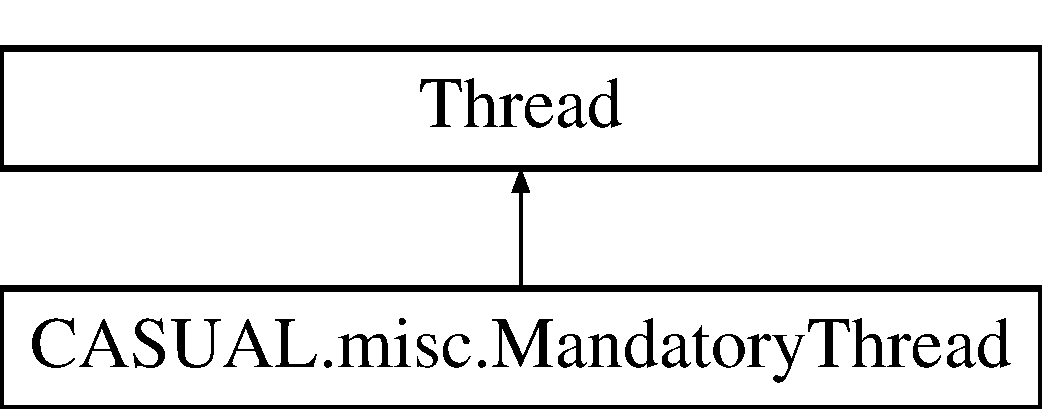
\includegraphics[height=2.000000cm]{classCASUAL_1_1misc_1_1MandatoryThread}
\end{center}
\end{figure}
\subsection*{Public Member Functions}
\begin{DoxyCompactItemize}
\item 
\hyperlink{classCASUAL_1_1misc_1_1MandatoryThread_a09160140c6e91ea2c5a14c264bc1fd85}{Mandatory\-Thread} ()
\item 
\hyperlink{classCASUAL_1_1misc_1_1MandatoryThread_ae74d0a4c148aa703b830d0890d666a7e}{Mandatory\-Thread} (Runnable r)
\item 
synchronized void \hyperlink{classCASUAL_1_1misc_1_1MandatoryThread_af99f45ee5d20c969c1d3edd167b334c7}{start} ()
\item 
boolean \hyperlink{classCASUAL_1_1misc_1_1MandatoryThread_af4c81c91c1927ed0f4fcab504ab2fe47}{is\-Complete} ()
\item 
synchronized void \hyperlink{classCASUAL_1_1misc_1_1MandatoryThread_a73dba51691a5c7a34fc584213e3a2121}{wait\-For} ()
\end{DoxyCompactItemize}


\subsection{Detailed Description}
\begin{DoxyAuthor}{Author}
adamoutler 
\end{DoxyAuthor}


\subsection{Constructor \& Destructor Documentation}
\hypertarget{classCASUAL_1_1misc_1_1MandatoryThread_a09160140c6e91ea2c5a14c264bc1fd85}{\index{C\-A\-S\-U\-A\-L\-::misc\-::\-Mandatory\-Thread@{C\-A\-S\-U\-A\-L\-::misc\-::\-Mandatory\-Thread}!Mandatory\-Thread@{Mandatory\-Thread}}
\index{Mandatory\-Thread@{Mandatory\-Thread}!CASUAL::misc::MandatoryThread@{C\-A\-S\-U\-A\-L\-::misc\-::\-Mandatory\-Thread}}
\subsubsection[{Mandatory\-Thread}]{\setlength{\rightskip}{0pt plus 5cm}C\-A\-S\-U\-A\-L.\-misc.\-Mandatory\-Thread.\-Mandatory\-Thread (
\begin{DoxyParamCaption}
{}
\end{DoxyParamCaption}
)}}\label{classCASUAL_1_1misc_1_1MandatoryThread_a09160140c6e91ea2c5a14c264bc1fd85}
constructor for thread sets up a blank Mandatory Thread. \hypertarget{classCASUAL_1_1misc_1_1MandatoryThread_ae74d0a4c148aa703b830d0890d666a7e}{\index{C\-A\-S\-U\-A\-L\-::misc\-::\-Mandatory\-Thread@{C\-A\-S\-U\-A\-L\-::misc\-::\-Mandatory\-Thread}!Mandatory\-Thread@{Mandatory\-Thread}}
\index{Mandatory\-Thread@{Mandatory\-Thread}!CASUAL::misc::MandatoryThread@{C\-A\-S\-U\-A\-L\-::misc\-::\-Mandatory\-Thread}}
\subsubsection[{Mandatory\-Thread}]{\setlength{\rightskip}{0pt plus 5cm}C\-A\-S\-U\-A\-L.\-misc.\-Mandatory\-Thread.\-Mandatory\-Thread (
\begin{DoxyParamCaption}
\item[{Runnable}]{r}
\end{DoxyParamCaption}
)}}\label{classCASUAL_1_1misc_1_1MandatoryThread_ae74d0a4c148aa703b830d0890d666a7e}
constructor accepts a runnable to be used for the thread. 
\begin{DoxyParams}{Parameters}
{\em r} & to be run in a different thread \\
\hline
\end{DoxyParams}


\subsection{Member Function Documentation}
\hypertarget{classCASUAL_1_1misc_1_1MandatoryThread_af4c81c91c1927ed0f4fcab504ab2fe47}{\index{C\-A\-S\-U\-A\-L\-::misc\-::\-Mandatory\-Thread@{C\-A\-S\-U\-A\-L\-::misc\-::\-Mandatory\-Thread}!is\-Complete@{is\-Complete}}
\index{is\-Complete@{is\-Complete}!CASUAL::misc::MandatoryThread@{C\-A\-S\-U\-A\-L\-::misc\-::\-Mandatory\-Thread}}
\subsubsection[{is\-Complete}]{\setlength{\rightskip}{0pt plus 5cm}boolean C\-A\-S\-U\-A\-L.\-misc.\-Mandatory\-Thread.\-is\-Complete (
\begin{DoxyParamCaption}
{}
\end{DoxyParamCaption}
)}}\label{classCASUAL_1_1misc_1_1MandatoryThread_af4c81c91c1927ed0f4fcab504ab2fe47}
is\-Complete allows for monitoring of the progress of a thread. If the thread has started and is no longer alive this will return true. The \hyperlink{classCASUAL_1_1misc_1_1MandatoryThread}{Mandatory\-Thread} has done its job. \begin{DoxyReturn}{Returns}
true if \hyperlink{classCASUAL_1_1misc_1_1MandatoryThread}{Mandatory\-Thread} is complete 
\end{DoxyReturn}
\hypertarget{classCASUAL_1_1misc_1_1MandatoryThread_af99f45ee5d20c969c1d3edd167b334c7}{\index{C\-A\-S\-U\-A\-L\-::misc\-::\-Mandatory\-Thread@{C\-A\-S\-U\-A\-L\-::misc\-::\-Mandatory\-Thread}!start@{start}}
\index{start@{start}!CASUAL::misc::MandatoryThread@{C\-A\-S\-U\-A\-L\-::misc\-::\-Mandatory\-Thread}}
\subsubsection[{start}]{\setlength{\rightskip}{0pt plus 5cm}synchronized void C\-A\-S\-U\-A\-L.\-misc.\-Mandatory\-Thread.\-start (
\begin{DoxyParamCaption}
{}
\end{DoxyParamCaption}
)}}\label{classCASUAL_1_1misc_1_1MandatoryThread_af99f45ee5d20c969c1d3edd167b334c7}
starts the thread and sets the \char`\"{}has\-Started\char`\"{} boolean. \hypertarget{classCASUAL_1_1misc_1_1MandatoryThread_a73dba51691a5c7a34fc584213e3a2121}{\index{C\-A\-S\-U\-A\-L\-::misc\-::\-Mandatory\-Thread@{C\-A\-S\-U\-A\-L\-::misc\-::\-Mandatory\-Thread}!wait\-For@{wait\-For}}
\index{wait\-For@{wait\-For}!CASUAL::misc::MandatoryThread@{C\-A\-S\-U\-A\-L\-::misc\-::\-Mandatory\-Thread}}
\subsubsection[{wait\-For}]{\setlength{\rightskip}{0pt plus 5cm}synchronized void C\-A\-S\-U\-A\-L.\-misc.\-Mandatory\-Thread.\-wait\-For (
\begin{DoxyParamCaption}
{}
\end{DoxyParamCaption}
)}}\label{classCASUAL_1_1misc_1_1MandatoryThread_a73dba51691a5c7a34fc584213e3a2121}
halts the current thread until the mandatory\-Thread has completed. If the thread has not started, it will wait for the thread to start. 

The documentation for this class was generated from the following file\-:\begin{DoxyCompactItemize}
\item 
trunk/\-C\-A\-S\-U\-A\-Lcore/src/\-C\-A\-S\-U\-A\-L/misc/Mandatory\-Thread.\-java\end{DoxyCompactItemize}

\hypertarget{classCASUAL_1_1crypto_1_1MD5sum}{\section{C\-A\-S\-U\-A\-L.\-crypto.\-M\-D5sum Class Reference}
\label{classCASUAL_1_1crypto_1_1MD5sum}\index{C\-A\-S\-U\-A\-L.\-crypto.\-M\-D5sum@{C\-A\-S\-U\-A\-L.\-crypto.\-M\-D5sum}}
}
\subsection*{Public Member Functions}
\begin{DoxyCompactItemize}
\item 
boolean \hyperlink{classCASUAL_1_1crypto_1_1MD5sum_a0179d638f6ae800b156ca5919e07abd9}{compare\-File\-To\-M\-D5} (File f, String M\-D5)
\item 
String \hyperlink{classCASUAL_1_1crypto_1_1MD5sum_ab4d622e3672fd560e125788e8c11da65}{md5sum} (Input\-Stream is)
\item 
String \hyperlink{classCASUAL_1_1crypto_1_1MD5sum_aba2245d66d6ca47b7bce88b31fec319d}{md5sum} (File f)
\item 
String \hyperlink{classCASUAL_1_1crypto_1_1MD5sum_ab3881ae275c9c2e89d3bbe0c20267f90}{md5sum\-Stream} (Input\-Stream is)
\item 
boolean \hyperlink{classCASUAL_1_1crypto_1_1MD5sum_a891774e4ad9bd42758f268cff8b99c1a}{compare\-M\-D5\-Strings\-From\-Linux\-Format\-To\-Filenames} (String\mbox{[}$\,$\mbox{]} Linux\-Format, String\mbox{[}$\,$\mbox{]} M\-D5\-Filenames)
\item 
\hypertarget{classCASUAL_1_1crypto_1_1MD5sum_a03e30cfb69b9e4edce983b18db357103}{String {\bfseries md5sum} (String string)}\label{classCASUAL_1_1crypto_1_1MD5sum_a03e30cfb69b9e4edce983b18db357103}

\item 
String\mbox{[}$\,$\mbox{]} \hyperlink{classCASUAL_1_1crypto_1_1MD5sum_a3ade14378f1ab5473e8cc4f9586a5b20}{split\-M\-D5\-String} (String md5)
\item 
String \hyperlink{classCASUAL_1_1crypto_1_1MD5sum_a6c175a3bfcc8ff9d9ccfdfe5570c6748}{get\-M\-D5from\-Linux\-M\-D5\-String} (String md5)
\item 
String \hyperlink{classCASUAL_1_1crypto_1_1MD5sum_ab47b5cec8ec08d6aef4fc80305644ea3}{get\-Linux\-M\-D5\-Sum} (File file)
\item 
String \hyperlink{classCASUAL_1_1crypto_1_1MD5sum_a99840f961574366d47cad9e5415cba0a}{get\-Linux\-M\-D5\-Sum} (Input\-Stream stream, String filename)
\item 
String \hyperlink{classCASUAL_1_1crypto_1_1MD5sum_a439b3e62c238ee0b72f4f13b552bf7a3}{get\-File\-Namefrom\-Linux\-M\-D5\-String} (String md5)
\item 
String \hyperlink{classCASUAL_1_1crypto_1_1MD5sum_a193a8d10d29e316913e9aa5a78707657}{convert\-M\-D5and\-Fileto\-Linux\-M\-D5\-Sum} (String md5, String filename)
\item 
boolean \hyperlink{classCASUAL_1_1crypto_1_1MD5sum_a95ab6e6c8e59044b302a7b5bf505211a}{line\-Contains\-M\-D5} (String test\-Line)
\item 
String \hyperlink{classCASUAL_1_1crypto_1_1MD5sum_a442e88f7440e8c11312bbb83318f6710}{pick\-New\-M\-D5from\-Array\-List} (Array\-List$<$ String $>$ new\-Md5\-List, String Old\-M\-D5)
\end{DoxyCompactItemize}


\subsection{Detailed Description}
\begin{DoxyAuthor}{Author}
adam 
\end{DoxyAuthor}


\subsection{Member Function Documentation}
\hypertarget{classCASUAL_1_1crypto_1_1MD5sum_a0179d638f6ae800b156ca5919e07abd9}{\index{C\-A\-S\-U\-A\-L\-::crypto\-::\-M\-D5sum@{C\-A\-S\-U\-A\-L\-::crypto\-::\-M\-D5sum}!compare\-File\-To\-M\-D5@{compare\-File\-To\-M\-D5}}
\index{compare\-File\-To\-M\-D5@{compare\-File\-To\-M\-D5}!CASUAL::crypto::MD5sum@{C\-A\-S\-U\-A\-L\-::crypto\-::\-M\-D5sum}}
\subsubsection[{compare\-File\-To\-M\-D5}]{\setlength{\rightskip}{0pt plus 5cm}boolean C\-A\-S\-U\-A\-L.\-crypto.\-M\-D5sum.\-compare\-File\-To\-M\-D5 (
\begin{DoxyParamCaption}
\item[{File}]{f, }
\item[{String}]{M\-D5}
\end{DoxyParamCaption}
)}}\label{classCASUAL_1_1crypto_1_1MD5sum_a0179d638f6ae800b156ca5919e07abd9}
compares an M\-D5 to a file


\begin{DoxyParams}{Parameters}
{\em f} & file to be compared \\
\hline
{\em M\-D5} & expected M\-D5 \\
\hline
\end{DoxyParams}
\begin{DoxyReturn}{Returns}
true if matches 
\end{DoxyReturn}
\hypertarget{classCASUAL_1_1crypto_1_1MD5sum_a891774e4ad9bd42758f268cff8b99c1a}{\index{C\-A\-S\-U\-A\-L\-::crypto\-::\-M\-D5sum@{C\-A\-S\-U\-A\-L\-::crypto\-::\-M\-D5sum}!compare\-M\-D5\-Strings\-From\-Linux\-Format\-To\-Filenames@{compare\-M\-D5\-Strings\-From\-Linux\-Format\-To\-Filenames}}
\index{compare\-M\-D5\-Strings\-From\-Linux\-Format\-To\-Filenames@{compare\-M\-D5\-Strings\-From\-Linux\-Format\-To\-Filenames}!CASUAL::crypto::MD5sum@{C\-A\-S\-U\-A\-L\-::crypto\-::\-M\-D5sum}}
\subsubsection[{compare\-M\-D5\-Strings\-From\-Linux\-Format\-To\-Filenames}]{\setlength{\rightskip}{0pt plus 5cm}boolean C\-A\-S\-U\-A\-L.\-crypto.\-M\-D5sum.\-compare\-M\-D5\-Strings\-From\-Linux\-Format\-To\-Filenames (
\begin{DoxyParamCaption}
\item[{String\mbox{[}$\,$\mbox{]}}]{Linux\-Format, }
\item[{String\mbox{[}$\,$\mbox{]}}]{M\-D5\-Filenames}
\end{DoxyParamCaption}
)}}\label{classCASUAL_1_1crypto_1_1MD5sum_a891774e4ad9bd42758f268cff8b99c1a}
compares files to M\-D5 to verify at least one matches


\begin{DoxyParams}{Parameters}
{\em Linux\-Format} & M\-D5 to compare \\
\hline
{\em M\-D5\-Filenames} & filenames to be checked \\
\hline
\end{DoxyParams}
\begin{DoxyReturn}{Returns}
true if all M\-D5s were matched to files 
\end{DoxyReturn}
\hypertarget{classCASUAL_1_1crypto_1_1MD5sum_a193a8d10d29e316913e9aa5a78707657}{\index{C\-A\-S\-U\-A\-L\-::crypto\-::\-M\-D5sum@{C\-A\-S\-U\-A\-L\-::crypto\-::\-M\-D5sum}!convert\-M\-D5and\-Fileto\-Linux\-M\-D5\-Sum@{convert\-M\-D5and\-Fileto\-Linux\-M\-D5\-Sum}}
\index{convert\-M\-D5and\-Fileto\-Linux\-M\-D5\-Sum@{convert\-M\-D5and\-Fileto\-Linux\-M\-D5\-Sum}!CASUAL::crypto::MD5sum@{C\-A\-S\-U\-A\-L\-::crypto\-::\-M\-D5sum}}
\subsubsection[{convert\-M\-D5and\-Fileto\-Linux\-M\-D5\-Sum}]{\setlength{\rightskip}{0pt plus 5cm}String C\-A\-S\-U\-A\-L.\-crypto.\-M\-D5sum.\-convert\-M\-D5and\-Fileto\-Linux\-M\-D5\-Sum (
\begin{DoxyParamCaption}
\item[{String}]{md5, }
\item[{String}]{filename}
\end{DoxyParamCaption}
)}}\label{classCASUAL_1_1crypto_1_1MD5sum_a193a8d10d29e316913e9aa5a78707657}
returns a standard md5sum


\begin{DoxyParams}{Parameters}
{\em md5} & md5 to be inserted \\
\hline
{\em filename} & filename to be appended \\
\hline
\end{DoxyParams}
\begin{DoxyReturn}{Returns}
linux md5sum 
\end{DoxyReturn}
\hypertarget{classCASUAL_1_1crypto_1_1MD5sum_a439b3e62c238ee0b72f4f13b552bf7a3}{\index{C\-A\-S\-U\-A\-L\-::crypto\-::\-M\-D5sum@{C\-A\-S\-U\-A\-L\-::crypto\-::\-M\-D5sum}!get\-File\-Namefrom\-Linux\-M\-D5\-String@{get\-File\-Namefrom\-Linux\-M\-D5\-String}}
\index{get\-File\-Namefrom\-Linux\-M\-D5\-String@{get\-File\-Namefrom\-Linux\-M\-D5\-String}!CASUAL::crypto::MD5sum@{C\-A\-S\-U\-A\-L\-::crypto\-::\-M\-D5sum}}
\subsubsection[{get\-File\-Namefrom\-Linux\-M\-D5\-String}]{\setlength{\rightskip}{0pt plus 5cm}String C\-A\-S\-U\-A\-L.\-crypto.\-M\-D5sum.\-get\-File\-Namefrom\-Linux\-M\-D5\-String (
\begin{DoxyParamCaption}
\item[{String}]{md5}
\end{DoxyParamCaption}
)}}\label{classCASUAL_1_1crypto_1_1MD5sum_a439b3e62c238ee0b72f4f13b552bf7a3}
gets filename from linux md5sum


\begin{DoxyParams}{Parameters}
{\em md5} & linux md5sum \\
\hline
\end{DoxyParams}
\begin{DoxyReturn}{Returns}
filename of md5sum input 
\end{DoxyReturn}
\hypertarget{classCASUAL_1_1crypto_1_1MD5sum_ab47b5cec8ec08d6aef4fc80305644ea3}{\index{C\-A\-S\-U\-A\-L\-::crypto\-::\-M\-D5sum@{C\-A\-S\-U\-A\-L\-::crypto\-::\-M\-D5sum}!get\-Linux\-M\-D5\-Sum@{get\-Linux\-M\-D5\-Sum}}
\index{get\-Linux\-M\-D5\-Sum@{get\-Linux\-M\-D5\-Sum}!CASUAL::crypto::MD5sum@{C\-A\-S\-U\-A\-L\-::crypto\-::\-M\-D5sum}}
\subsubsection[{get\-Linux\-M\-D5\-Sum}]{\setlength{\rightskip}{0pt plus 5cm}String C\-A\-S\-U\-A\-L.\-crypto.\-M\-D5sum.\-get\-Linux\-M\-D5\-Sum (
\begin{DoxyParamCaption}
\item[{File}]{file}
\end{DoxyParamCaption}
)}}\label{classCASUAL_1_1crypto_1_1MD5sum_ab47b5cec8ec08d6aef4fc80305644ea3}
Returns the standard md5sum found on Linux as though the file were in the same directory


\begin{DoxyParams}{Parameters}
{\em file} & to be \hyperlink{classCASUAL_1_1crypto_1_1MD5sum}{M\-D5sum}'d \\
\hline
\end{DoxyParams}
\begin{DoxyReturn}{Returns}
32digit\-Md5\-Sum+\char`\"{} \char`\"{}+file.Name 
\end{DoxyReturn}
\hypertarget{classCASUAL_1_1crypto_1_1MD5sum_a99840f961574366d47cad9e5415cba0a}{\index{C\-A\-S\-U\-A\-L\-::crypto\-::\-M\-D5sum@{C\-A\-S\-U\-A\-L\-::crypto\-::\-M\-D5sum}!get\-Linux\-M\-D5\-Sum@{get\-Linux\-M\-D5\-Sum}}
\index{get\-Linux\-M\-D5\-Sum@{get\-Linux\-M\-D5\-Sum}!CASUAL::crypto::MD5sum@{C\-A\-S\-U\-A\-L\-::crypto\-::\-M\-D5sum}}
\subsubsection[{get\-Linux\-M\-D5\-Sum}]{\setlength{\rightskip}{0pt plus 5cm}String C\-A\-S\-U\-A\-L.\-crypto.\-M\-D5sum.\-get\-Linux\-M\-D5\-Sum (
\begin{DoxyParamCaption}
\item[{Input\-Stream}]{stream, }
\item[{String}]{filename}
\end{DoxyParamCaption}
)}}\label{classCASUAL_1_1crypto_1_1MD5sum_a99840f961574366d47cad9e5415cba0a}
Returns the standard md5sum found on Linux as though the file were in the same directory


\begin{DoxyParams}{Parameters}
{\em stream} & to be \hyperlink{classCASUAL_1_1crypto_1_1MD5sum}{M\-D5sum}'d \\
\hline
{\em filename} & to append to the stream \\
\hline
\end{DoxyParams}
\begin{DoxyReturn}{Returns}
32digit\-Md5\-Sum+\char`\"{} \char`\"{}+file.Name 
\end{DoxyReturn}
\hypertarget{classCASUAL_1_1crypto_1_1MD5sum_a6c175a3bfcc8ff9d9ccfdfe5570c6748}{\index{C\-A\-S\-U\-A\-L\-::crypto\-::\-M\-D5sum@{C\-A\-S\-U\-A\-L\-::crypto\-::\-M\-D5sum}!get\-M\-D5from\-Linux\-M\-D5\-String@{get\-M\-D5from\-Linux\-M\-D5\-String}}
\index{get\-M\-D5from\-Linux\-M\-D5\-String@{get\-M\-D5from\-Linux\-M\-D5\-String}!CASUAL::crypto::MD5sum@{C\-A\-S\-U\-A\-L\-::crypto\-::\-M\-D5sum}}
\subsubsection[{get\-M\-D5from\-Linux\-M\-D5\-String}]{\setlength{\rightskip}{0pt plus 5cm}String C\-A\-S\-U\-A\-L.\-crypto.\-M\-D5sum.\-get\-M\-D5from\-Linux\-M\-D5\-String (
\begin{DoxyParamCaption}
\item[{String}]{md5}
\end{DoxyParamCaption}
)}}\label{classCASUAL_1_1crypto_1_1MD5sum_a6c175a3bfcc8ff9d9ccfdfe5570c6748}
returns M\-D5 from a linux md5sum


\begin{DoxyParams}{Parameters}
{\em md5} & linux \hyperlink{classCASUAL_1_1crypto_1_1MD5sum}{M\-D5sum} \\
\hline
\end{DoxyParams}
\begin{DoxyReturn}{Returns}
md5 
\end{DoxyReturn}
\hypertarget{classCASUAL_1_1crypto_1_1MD5sum_a95ab6e6c8e59044b302a7b5bf505211a}{\index{C\-A\-S\-U\-A\-L\-::crypto\-::\-M\-D5sum@{C\-A\-S\-U\-A\-L\-::crypto\-::\-M\-D5sum}!line\-Contains\-M\-D5@{line\-Contains\-M\-D5}}
\index{line\-Contains\-M\-D5@{line\-Contains\-M\-D5}!CASUAL::crypto::MD5sum@{C\-A\-S\-U\-A\-L\-::crypto\-::\-M\-D5sum}}
\subsubsection[{line\-Contains\-M\-D5}]{\setlength{\rightskip}{0pt plus 5cm}boolean C\-A\-S\-U\-A\-L.\-crypto.\-M\-D5sum.\-line\-Contains\-M\-D5 (
\begin{DoxyParamCaption}
\item[{String}]{test\-Line}
\end{DoxyParamCaption}
)}}\label{classCASUAL_1_1crypto_1_1MD5sum_a95ab6e6c8e59044b302a7b5bf505211a}
tests to see if a line matches an md5sum


\begin{DoxyParams}{Parameters}
{\em test\-Line} & line in question \\
\hline
\end{DoxyParams}
\begin{DoxyReturn}{Returns}
true if this is contains a 32 byte hex string 
\end{DoxyReturn}
\hypertarget{classCASUAL_1_1crypto_1_1MD5sum_ab4d622e3672fd560e125788e8c11da65}{\index{C\-A\-S\-U\-A\-L\-::crypto\-::\-M\-D5sum@{C\-A\-S\-U\-A\-L\-::crypto\-::\-M\-D5sum}!md5sum@{md5sum}}
\index{md5sum@{md5sum}!CASUAL::crypto::MD5sum@{C\-A\-S\-U\-A\-L\-::crypto\-::\-M\-D5sum}}
\subsubsection[{md5sum}]{\setlength{\rightskip}{0pt plus 5cm}String C\-A\-S\-U\-A\-L.\-crypto.\-M\-D5sum.\-md5sum (
\begin{DoxyParamCaption}
\item[{Input\-Stream}]{is}
\end{DoxyParamCaption}
)}}\label{classCASUAL_1_1crypto_1_1MD5sum_ab4d622e3672fd560e125788e8c11da65}
gets M\-D5 of input stream


\begin{DoxyParams}{Parameters}
{\em is} & stream to be M\-D5d \\
\hline
\end{DoxyParams}
\begin{DoxyReturn}{Returns}
md5 of stream 
\end{DoxyReturn}
\hypertarget{classCASUAL_1_1crypto_1_1MD5sum_aba2245d66d6ca47b7bce88b31fec319d}{\index{C\-A\-S\-U\-A\-L\-::crypto\-::\-M\-D5sum@{C\-A\-S\-U\-A\-L\-::crypto\-::\-M\-D5sum}!md5sum@{md5sum}}
\index{md5sum@{md5sum}!CASUAL::crypto::MD5sum@{C\-A\-S\-U\-A\-L\-::crypto\-::\-M\-D5sum}}
\subsubsection[{md5sum}]{\setlength{\rightskip}{0pt plus 5cm}String C\-A\-S\-U\-A\-L.\-crypto.\-M\-D5sum.\-md5sum (
\begin{DoxyParamCaption}
\item[{File}]{f}
\end{DoxyParamCaption}
)}}\label{classCASUAL_1_1crypto_1_1MD5sum_aba2245d66d6ca47b7bce88b31fec319d}
M\-D5s a file


\begin{DoxyParams}{Parameters}
{\em f} & file to M\-D5 \\
\hline
\end{DoxyParams}
\begin{DoxyReturn}{Returns}
md5 of file 
\end{DoxyReturn}
\hypertarget{classCASUAL_1_1crypto_1_1MD5sum_ab3881ae275c9c2e89d3bbe0c20267f90}{\index{C\-A\-S\-U\-A\-L\-::crypto\-::\-M\-D5sum@{C\-A\-S\-U\-A\-L\-::crypto\-::\-M\-D5sum}!md5sum\-Stream@{md5sum\-Stream}}
\index{md5sum\-Stream@{md5sum\-Stream}!CASUAL::crypto::MD5sum@{C\-A\-S\-U\-A\-L\-::crypto\-::\-M\-D5sum}}
\subsubsection[{md5sum\-Stream}]{\setlength{\rightskip}{0pt plus 5cm}String C\-A\-S\-U\-A\-L.\-crypto.\-M\-D5sum.\-md5sum\-Stream (
\begin{DoxyParamCaption}
\item[{Input\-Stream}]{is}
\end{DoxyParamCaption}
)}}\label{classCASUAL_1_1crypto_1_1MD5sum_ab3881ae275c9c2e89d3bbe0c20267f90}
md5s an input stream


\begin{DoxyParams}{Parameters}
{\em is} & stream to M\-D5 \\
\hline
\end{DoxyParams}
\begin{DoxyReturn}{Returns}
md5 of stream 
\end{DoxyReturn}
\hypertarget{classCASUAL_1_1crypto_1_1MD5sum_a442e88f7440e8c11312bbb83318f6710}{\index{C\-A\-S\-U\-A\-L\-::crypto\-::\-M\-D5sum@{C\-A\-S\-U\-A\-L\-::crypto\-::\-M\-D5sum}!pick\-New\-M\-D5from\-Array\-List@{pick\-New\-M\-D5from\-Array\-List}}
\index{pick\-New\-M\-D5from\-Array\-List@{pick\-New\-M\-D5from\-Array\-List}!CASUAL::crypto::MD5sum@{C\-A\-S\-U\-A\-L\-::crypto\-::\-M\-D5sum}}
\subsubsection[{pick\-New\-M\-D5from\-Array\-List}]{\setlength{\rightskip}{0pt plus 5cm}String C\-A\-S\-U\-A\-L.\-crypto.\-M\-D5sum.\-pick\-New\-M\-D5from\-Array\-List (
\begin{DoxyParamCaption}
\item[{Array\-List$<$ String $>$}]{new\-Md5\-List, }
\item[{String}]{Old\-M\-D5}
\end{DoxyParamCaption}
)}}\label{classCASUAL_1_1crypto_1_1MD5sum_a442e88f7440e8c11312bbb83318f6710}
picks the new M\-D5 if available


\begin{DoxyParams}{Parameters}
{\em new\-Md5\-List} & new M\-D5s \\
\hline
{\em Old\-M\-D5} & old md5s \\
\hline
\end{DoxyParams}
\begin{DoxyReturn}{Returns}
new md5s if available 
\end{DoxyReturn}
\hypertarget{classCASUAL_1_1crypto_1_1MD5sum_a3ade14378f1ab5473e8cc4f9586a5b20}{\index{C\-A\-S\-U\-A\-L\-::crypto\-::\-M\-D5sum@{C\-A\-S\-U\-A\-L\-::crypto\-::\-M\-D5sum}!split\-M\-D5\-String@{split\-M\-D5\-String}}
\index{split\-M\-D5\-String@{split\-M\-D5\-String}!CASUAL::crypto::MD5sum@{C\-A\-S\-U\-A\-L\-::crypto\-::\-M\-D5sum}}
\subsubsection[{split\-M\-D5\-String}]{\setlength{\rightskip}{0pt plus 5cm}String \mbox{[}$\,$\mbox{]} C\-A\-S\-U\-A\-L.\-crypto.\-M\-D5sum.\-split\-M\-D5\-String (
\begin{DoxyParamCaption}
\item[{String}]{md5}
\end{DoxyParamCaption}
)}}\label{classCASUAL_1_1crypto_1_1MD5sum_a3ade14378f1ab5473e8cc4f9586a5b20}
splits a Linux \hyperlink{classCASUAL_1_1crypto_1_1MD5sum}{M\-D5sum} value into a md5 and a filename


\begin{DoxyParams}{Parameters}
{\em md5} & linux md5 sum \\
\hline
\end{DoxyParams}
\begin{DoxyReturn}{Returns}
md5,filename 
\end{DoxyReturn}


The documentation for this class was generated from the following file\-:\begin{DoxyCompactItemize}
\item 
trunk/\-C\-A\-S\-U\-A\-Lcore/src/\-C\-A\-S\-U\-A\-L/crypto/M\-D5sum.\-java\end{DoxyCompactItemize}

\hypertarget{classCASUAL_1_1crypto_1_1MD5sumTest}{\section{C\-A\-S\-U\-A\-L.\-crypto.\-M\-D5sum\-Test Class Reference}
\label{classCASUAL_1_1crypto_1_1MD5sumTest}\index{C\-A\-S\-U\-A\-L.\-crypto.\-M\-D5sum\-Test@{C\-A\-S\-U\-A\-L.\-crypto.\-M\-D5sum\-Test}}
}
\subsection*{Public Member Functions}
\begin{DoxyCompactItemize}
\item 
\hypertarget{classCASUAL_1_1crypto_1_1MD5sumTest_a03b77b8c2dbe1c4566d288d7b92c7d56}{void {\bfseries set\-Up} ()}\label{classCASUAL_1_1crypto_1_1MD5sumTest_a03b77b8c2dbe1c4566d288d7b92c7d56}

\item 
\hypertarget{classCASUAL_1_1crypto_1_1MD5sumTest_a90b541e86a5e7b31e8033e9e5a2a69a0}{void {\bfseries test\-Md5sum\-\_\-\-Input\-Stream} ()}\label{classCASUAL_1_1crypto_1_1MD5sumTest_a90b541e86a5e7b31e8033e9e5a2a69a0}

\end{DoxyCompactItemize}


\subsection{Detailed Description}
\begin{DoxyAuthor}{Author}
adam 
\end{DoxyAuthor}


The documentation for this class was generated from the following file\-:\begin{DoxyCompactItemize}
\item 
trunk/\-C\-A\-S\-U\-A\-Lcore/test/\-C\-A\-S\-U\-A\-L/crypto/M\-D5sum\-Test.\-java\end{DoxyCompactItemize}

\hypertarget{classCASUAL_1_1caspac_1_1Script_1_1meta}{\section{C\-A\-S\-U\-A\-L.\-caspac.\-Script.\-meta Class Reference}
\label{classCASUAL_1_1caspac_1_1Script_1_1meta}\index{C\-A\-S\-U\-A\-L.\-caspac.\-Script.\-meta@{C\-A\-S\-U\-A\-L.\-caspac.\-Script.\-meta}}
}
\subsection*{Public Member Functions}
\begin{DoxyCompactItemize}
\item 
\hypertarget{classCASUAL_1_1caspac_1_1Script_1_1meta_a261edd605871c12eae55492b767f5d91}{{\bfseries meta} (Properties prop)}\label{classCASUAL_1_1caspac_1_1Script_1_1meta_a261edd605871c12eae55492b767f5d91}

\item 
\hypertarget{classCASUAL_1_1caspac_1_1Script_1_1meta_a82642004af42f27e39b25701f959366c}{{\bfseries meta} (Input\-Stream prop)  throws I\-O\-Exception }\label{classCASUAL_1_1caspac_1_1Script_1_1meta_a82642004af42f27e39b25701f959366c}

\item 
boolean \hyperlink{classCASUAL_1_1caspac_1_1Script_1_1meta_a4340eebaf11efe0a5be240ac719287c9}{verify\-Meta} ()
\item 
\hypertarget{classCASUAL_1_1caspac_1_1Script_1_1meta_ac00ebebaaa934593f664e4f8a992dac1}{Input\-Stream {\bfseries get\-Meta\-Input\-Stream} ()}\label{classCASUAL_1_1caspac_1_1Script_1_1meta_ac00ebebaaa934593f664e4f8a992dac1}

\item 
boolean \hyperlink{classCASUAL_1_1caspac_1_1Script_1_1meta_abd994423729ec381ff3d2ce236981533}{write} (String output)  throws File\-Not\-Found\-Exception, I\-O\-Exception 
\item 
boolean \hyperlink{classCASUAL_1_1caspac_1_1Script_1_1meta_a24fe150d261aea726080f70c0403a81e}{write} (File output)  throws File\-Not\-Found\-Exception, I\-O\-Exception 
\item 
void \hyperlink{classCASUAL_1_1caspac_1_1Script_1_1meta_a356836bc34bf0e4bc68ee064277660db}{set\-Props\-From\-Variables} ()
\item 
\hypertarget{classCASUAL_1_1caspac_1_1Script_1_1meta_a2d21562b3e0b7d4fcdb1089817ab9eca}{void {\bfseries load} (Properties prop)}\label{classCASUAL_1_1caspac_1_1Script_1_1meta_a2d21562b3e0b7d4fcdb1089817ab9eca}

\item 
\hypertarget{classCASUAL_1_1caspac_1_1Script_1_1meta_a451f01951a3e308647fc725fdcc50b7d}{int {\bfseries min\-S\-V\-Nversion} ()}\label{classCASUAL_1_1caspac_1_1Script_1_1meta_a451f01951a3e308647fc725fdcc50b7d}

\end{DoxyCompactItemize}
\subsection*{Public Attributes}
\begin{DoxyCompactItemize}
\item 
\hypertarget{classCASUAL_1_1caspac_1_1Script_1_1meta_ae1e5528a05bcf7cbc7f368017a7e7ab7}{String {\bfseries min\-S\-V\-Nversion} = \char`\"{}\char`\"{}}\label{classCASUAL_1_1caspac_1_1Script_1_1meta_ae1e5528a05bcf7cbc7f368017a7e7ab7}

\item 
\hypertarget{classCASUAL_1_1caspac_1_1Script_1_1meta_a1a3e2319baaf7bb61c7eaaf6b1171a2f}{String {\bfseries script\-Revision} = \char`\"{}\char`\"{}}\label{classCASUAL_1_1caspac_1_1Script_1_1meta_a1a3e2319baaf7bb61c7eaaf6b1171a2f}

\item 
\hypertarget{classCASUAL_1_1caspac_1_1Script_1_1meta_a66dee5c26c32cfdf3946df4cc196e433}{String {\bfseries unique\-Identifier} = \char`\"{}\char`\"{}}\label{classCASUAL_1_1caspac_1_1Script_1_1meta_a66dee5c26c32cfdf3946df4cc196e433}

\item 
\hypertarget{classCASUAL_1_1caspac_1_1Script_1_1meta_a071a5d2bbbebdb096a336741a86bd1a1}{String {\bfseries support\-U\-R\-L} = \char`\"{}\char`\"{}}\label{classCASUAL_1_1caspac_1_1Script_1_1meta_a071a5d2bbbebdb096a336741a86bd1a1}

\item 
\hypertarget{classCASUAL_1_1caspac_1_1Script_1_1meta_a4b493e05ac7a0fa575a524b9caa22de9}{String {\bfseries update\-Message} = \char`\"{}\char`\"{}}\label{classCASUAL_1_1caspac_1_1Script_1_1meta_a4b493e05ac7a0fa575a524b9caa22de9}

\item 
\hypertarget{classCASUAL_1_1caspac_1_1Script_1_1meta_ac2d935e89f56476aa42981a2f5234006}{String {\bfseries kill\-Switch\-Message} = \char`\"{}\char`\"{}}\label{classCASUAL_1_1caspac_1_1Script_1_1meta_ac2d935e89f56476aa42981a2f5234006}

\item 
\hypertarget{classCASUAL_1_1caspac_1_1Script_1_1meta_a7ac1b9733ee7c804910d73774d4c4fdd}{Properties {\bfseries meta\-Prop}}\label{classCASUAL_1_1caspac_1_1Script_1_1meta_a7ac1b9733ee7c804910d73774d4c4fdd}

\item 
\hypertarget{classCASUAL_1_1caspac_1_1Script_1_1meta_a168fec9801221d6f93058c8c254f3747}{List$<$ String $>$ {\bfseries md5s} = new Array\-List$<$String$>$()}\label{classCASUAL_1_1caspac_1_1Script_1_1meta_a168fec9801221d6f93058c8c254f3747}

\end{DoxyCompactItemize}


\subsection{Member Function Documentation}
\hypertarget{classCASUAL_1_1caspac_1_1Script_1_1meta_a356836bc34bf0e4bc68ee064277660db}{\index{C\-A\-S\-U\-A\-L\-::caspac\-::\-Script\-::meta@{C\-A\-S\-U\-A\-L\-::caspac\-::\-Script\-::meta}!set\-Props\-From\-Variables@{set\-Props\-From\-Variables}}
\index{set\-Props\-From\-Variables@{set\-Props\-From\-Variables}!CASUAL::caspac::Script::meta@{C\-A\-S\-U\-A\-L\-::caspac\-::\-Script\-::meta}}
\subsubsection[{set\-Props\-From\-Variables}]{\setlength{\rightskip}{0pt plus 5cm}void C\-A\-S\-U\-A\-L.\-caspac.\-Script.\-meta.\-set\-Props\-From\-Variables (
\begin{DoxyParamCaption}
{}
\end{DoxyParamCaption}
)}}\label{classCASUAL_1_1caspac_1_1Script_1_1meta_a356836bc34bf0e4bc68ee064277660db}
sets the properties object from local variables for writing \hypertarget{classCASUAL_1_1caspac_1_1Script_1_1meta_a4340eebaf11efe0a5be240ac719287c9}{\index{C\-A\-S\-U\-A\-L\-::caspac\-::\-Script\-::meta@{C\-A\-S\-U\-A\-L\-::caspac\-::\-Script\-::meta}!verify\-Meta@{verify\-Meta}}
\index{verify\-Meta@{verify\-Meta}!CASUAL::caspac::Script::meta@{C\-A\-S\-U\-A\-L\-::caspac\-::\-Script\-::meta}}
\subsubsection[{verify\-Meta}]{\setlength{\rightskip}{0pt plus 5cm}boolean C\-A\-S\-U\-A\-L.\-caspac.\-Script.\-meta.\-verify\-Meta (
\begin{DoxyParamCaption}
{}
\end{DoxyParamCaption}
)}}\label{classCASUAL_1_1caspac_1_1Script_1_1meta_a4340eebaf11efe0a5be240ac719287c9}
verifies metadata is not empty

\begin{DoxyReturn}{Returns}
true if filled in 
\end{DoxyReturn}
\hypertarget{classCASUAL_1_1caspac_1_1Script_1_1meta_abd994423729ec381ff3d2ce236981533}{\index{C\-A\-S\-U\-A\-L\-::caspac\-::\-Script\-::meta@{C\-A\-S\-U\-A\-L\-::caspac\-::\-Script\-::meta}!write@{write}}
\index{write@{write}!CASUAL::caspac::Script::meta@{C\-A\-S\-U\-A\-L\-::caspac\-::\-Script\-::meta}}
\subsubsection[{write}]{\setlength{\rightskip}{0pt plus 5cm}boolean C\-A\-S\-U\-A\-L.\-caspac.\-Script.\-meta.\-write (
\begin{DoxyParamCaption}
\item[{String}]{output}
\end{DoxyParamCaption}
) throws File\-Not\-Found\-Exception, I\-O\-Exception}}\label{classCASUAL_1_1caspac_1_1Script_1_1meta_abd994423729ec381ff3d2ce236981533}
writes meta properties to a file


\begin{DoxyParams}{Parameters}
{\em output} & file to write \\
\hline
\end{DoxyParams}
\begin{DoxyReturn}{Returns}
true if file was written 
\end{DoxyReturn}

\begin{DoxyExceptions}{Exceptions}
{\em File\-Not\-Found\-Exception} & \\
\hline
{\em I\-O\-Exception} & \\
\hline
\end{DoxyExceptions}
\hypertarget{classCASUAL_1_1caspac_1_1Script_1_1meta_a24fe150d261aea726080f70c0403a81e}{\index{C\-A\-S\-U\-A\-L\-::caspac\-::\-Script\-::meta@{C\-A\-S\-U\-A\-L\-::caspac\-::\-Script\-::meta}!write@{write}}
\index{write@{write}!CASUAL::caspac::Script::meta@{C\-A\-S\-U\-A\-L\-::caspac\-::\-Script\-::meta}}
\subsubsection[{write}]{\setlength{\rightskip}{0pt plus 5cm}boolean C\-A\-S\-U\-A\-L.\-caspac.\-Script.\-meta.\-write (
\begin{DoxyParamCaption}
\item[{File}]{output}
\end{DoxyParamCaption}
) throws File\-Not\-Found\-Exception, I\-O\-Exception}}\label{classCASUAL_1_1caspac_1_1Script_1_1meta_a24fe150d261aea726080f70c0403a81e}
writes meta properties to a file


\begin{DoxyParams}{Parameters}
{\em output} & file to write \\
\hline
\end{DoxyParams}
\begin{DoxyReturn}{Returns}
true if file was written 
\end{DoxyReturn}

\begin{DoxyExceptions}{Exceptions}
{\em File\-Not\-Found\-Exception} & \\
\hline
{\em I\-O\-Exception} & \\
\hline
\end{DoxyExceptions}


The documentation for this class was generated from the following file\-:\begin{DoxyCompactItemize}
\item 
trunk/\-C\-A\-S\-U\-A\-Lcore/src/\-C\-A\-S\-U\-A\-L/caspac/Script.\-java\end{DoxyCompactItemize}

\hypertarget{classdevicedetector_1_1msiexecInterface}{\section{devicedetector.\-msiexec\-Interface Class Reference}
\label{classdevicedetector_1_1msiexecInterface}\index{devicedetector.\-msiexec\-Interface@{devicedetector.\-msiexec\-Interface}}
}
\subsection*{Classes}
\begin{DoxyCompactItemize}
\item 
enum \hyperlink{enumdevicedetector_1_1msiexecInterface_1_1LoggingOption}{Logging\-Option}
\item 
enum \hyperlink{enumdevicedetector_1_1msiexecInterface_1_1Operation}{Operation}
\item 
enum \hyperlink{enumdevicedetector_1_1msiexecInterface_1_1RepairOptions}{Repair\-Options}
\end{DoxyCompactItemize}
\subsection*{Public Member Functions}
\begin{DoxyCompactItemize}
\item 
\hypertarget{classdevicedetector_1_1msiexecInterface_a2fa2fd5b5c65cd60a45327d4c145bd0e}{{\bfseries msiexec\-Interface} (String msi\-File)}\label{classdevicedetector_1_1msiexecInterface_a2fa2fd5b5c65cd60a45327d4c145bd0e}

\item 
\hypertarget{classdevicedetector_1_1msiexecInterface_a2e3d833fcace173477e58429bc78ece6}{\hyperlink{enumdevicedetector_1_1msiexecInterface_1_1Operation}{Operation} {\bfseries get\-Op} ()}\label{classdevicedetector_1_1msiexecInterface_a2e3d833fcace173477e58429bc78ece6}

\item 
\hypertarget{classdevicedetector_1_1msiexecInterface_a692737e5312ae114ae40366780edf558}{void {\bfseries set\-Op} (\hyperlink{enumdevicedetector_1_1msiexecInterface_1_1Operation}{Operation} op)}\label{classdevicedetector_1_1msiexecInterface_a692737e5312ae114ae40366780edf558}

\item 
\hypertarget{classdevicedetector_1_1msiexecInterface_a3b2524c031cf8700cfc4183cfc094030}{\hyperlink{enumdevicedetector_1_1msiexecInterface_1_1RepairOptions}{Repair\-Options} {\bfseries get\-Ro} ()}\label{classdevicedetector_1_1msiexecInterface_a3b2524c031cf8700cfc4183cfc094030}

\item 
\hypertarget{classdevicedetector_1_1msiexecInterface_a050ab718c79eb8169a3d77a55a8223d6}{void {\bfseries set\-Ro} (\hyperlink{enumdevicedetector_1_1msiexecInterface_1_1RepairOptions}{Repair\-Options} ro)}\label{classdevicedetector_1_1msiexecInterface_a050ab718c79eb8169a3d77a55a8223d6}

\item 
\hypertarget{classdevicedetector_1_1msiexecInterface_ae2acafaed9a25f4bf743e4e81d3f1e98}{boolean {\bfseries is\-Quite} ()}\label{classdevicedetector_1_1msiexecInterface_ae2acafaed9a25f4bf743e4e81d3f1e98}

\item 
\hypertarget{classdevicedetector_1_1msiexecInterface_a6ae9285d9ea7c3413680745457dcc1cc}{void {\bfseries set\-Quite} (boolean quite)}\label{classdevicedetector_1_1msiexecInterface_a6ae9285d9ea7c3413680745457dcc1cc}

\item 
\hypertarget{classdevicedetector_1_1msiexecInterface_ae2e377d5d86f2f9f8c4f469f77083773}{boolean {\bfseries is\-Logging} ()}\label{classdevicedetector_1_1msiexecInterface_ae2e377d5d86f2f9f8c4f469f77083773}

\item 
\hypertarget{classdevicedetector_1_1msiexecInterface_ae440fe69f727c62f65f1c196ed401893}{void {\bfseries set\-Logging} (boolean logging)}\label{classdevicedetector_1_1msiexecInterface_ae440fe69f727c62f65f1c196ed401893}

\item 
\hypertarget{classdevicedetector_1_1msiexecInterface_a8b0d8f54ad5aff52e4a0801d9bf17894}{File {\bfseries get\-Log\-File} ()}\label{classdevicedetector_1_1msiexecInterface_a8b0d8f54ad5aff52e4a0801d9bf17894}

\item 
\hypertarget{classdevicedetector_1_1msiexecInterface_a547e4241f3b3b88415fcf21d9ebd1dd2}{void {\bfseries set\-Log\-File} (File log\-File)}\label{classdevicedetector_1_1msiexecInterface_a547e4241f3b3b88415fcf21d9ebd1dd2}

\item 
\hypertarget{classdevicedetector_1_1msiexecInterface_a72063d1db13e102033b5e8edfa931145}{Enum\-Map$<$ \hyperlink{enumdevicedetector_1_1msiexecInterface_1_1LoggingOption}{Logging\-Option}, String $>$ {\bfseries get\-Logging\-Options} ()}\label{classdevicedetector_1_1msiexecInterface_a72063d1db13e102033b5e8edfa931145}

\item 
\hypertarget{classdevicedetector_1_1msiexecInterface_a79c9dae90ed7451077cdceb03c1a5cac}{void {\bfseries set\-Logging\-Options} (Logging\-Option...\-logging\-Options)}\label{classdevicedetector_1_1msiexecInterface_a79c9dae90ed7451077cdceb03c1a5cac}

\end{DoxyCompactItemize}
\subsection*{Static Public Member Functions}
\begin{DoxyCompactItemize}
\item 
\hypertarget{classdevicedetector_1_1msiexecInterface_a0700312a7d2281b1cddfbf2f3d9f57f2}{static void {\bfseries main} (String\mbox{[}$\,$\mbox{]} args)}\label{classdevicedetector_1_1msiexecInterface_a0700312a7d2281b1cddfbf2f3d9f57f2}

\end{DoxyCompactItemize}
\subsection*{Public Attributes}
\begin{DoxyCompactItemize}
\item 
\hypertarget{classdevicedetector_1_1msiexecInterface_a37415cd16a018c25018fef73000e74b9}{boolean {\bfseries quite} = true}\label{classdevicedetector_1_1msiexecInterface_a37415cd16a018c25018fef73000e74b9}

\item 
\hypertarget{classdevicedetector_1_1msiexecInterface_abdcbd5d14dadae4d73226f19c986356d}{File {\bfseries log\-File}}\label{classdevicedetector_1_1msiexecInterface_abdcbd5d14dadae4d73226f19c986356d}

\end{DoxyCompactItemize}


\subsection{Detailed Description}
\begin{DoxyAuthor}{Author}
loganludington 
\end{DoxyAuthor}


The documentation for this class was generated from the following file\-:\begin{DoxyCompactItemize}
\item 
branches/\-Testing\-Branch/\-Device\-Detector/src/devicedetector/msiexec\-Interface.\-java\end{DoxyCompactItemize}

\hypertarget{classCASUAL_1_1misc_1_1MultiClassLoader}{\section{C\-A\-S\-U\-A\-L.\-misc.\-Multi\-Class\-Loader Class Reference}
\label{classCASUAL_1_1misc_1_1MultiClassLoader}\index{C\-A\-S\-U\-A\-L.\-misc.\-Multi\-Class\-Loader@{C\-A\-S\-U\-A\-L.\-misc.\-Multi\-Class\-Loader}}
}
Inheritance diagram for C\-A\-S\-U\-A\-L.\-misc.\-Multi\-Class\-Loader\-:\begin{figure}[H]
\begin{center}
\leavevmode
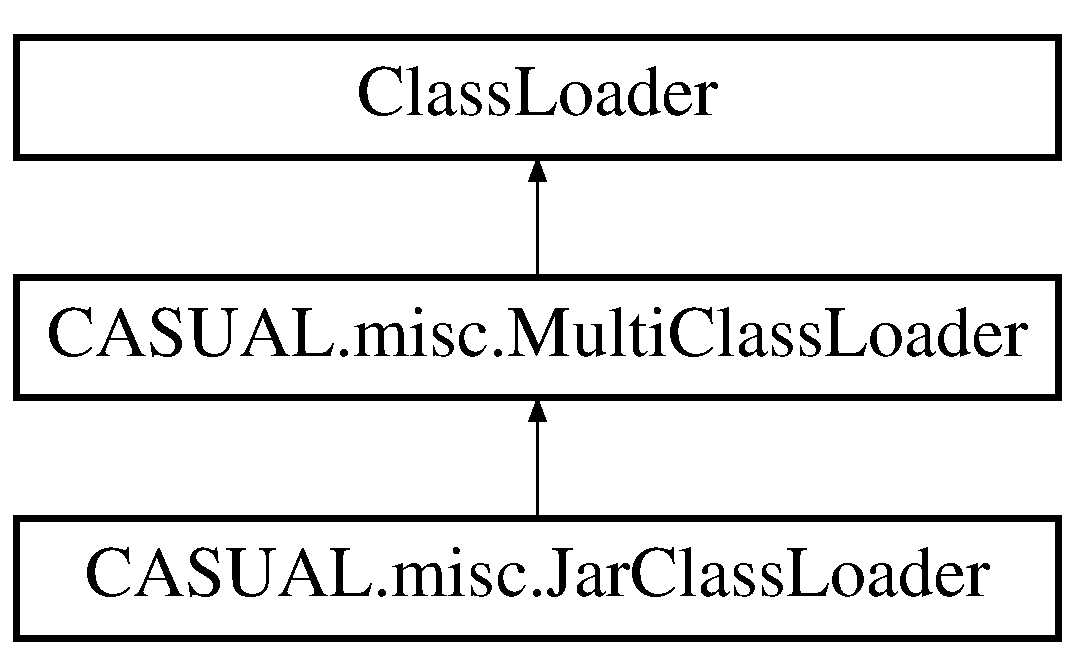
\includegraphics[height=3.000000cm]{classCASUAL_1_1misc_1_1MultiClassLoader}
\end{center}
\end{figure}
\subsection*{Public Member Functions}
\begin{DoxyCompactItemize}
\item 
Class \hyperlink{classCASUAL_1_1misc_1_1MultiClassLoader_a55eb86977110bf1b756eb0d3fb4fd94e}{load\-Class} (String class\-Name)  throws Class\-Not\-Found\-Exception 
\item 
\hypertarget{classCASUAL_1_1misc_1_1MultiClassLoader_abff00159b724689d0be2e0b927a591b4}{synchronized Class {\bfseries load\-Class} (String class\-Name, boolean resolve\-It)  throws Class\-Not\-Found\-Exception }\label{classCASUAL_1_1misc_1_1MultiClassLoader_abff00159b724689d0be2e0b927a591b4}

\item 
void \hyperlink{classCASUAL_1_1misc_1_1MultiClassLoader_a185926422f007e59628c04e199596b36}{set\-Class\-Name\-Replacement\-Char} (char replacement)
\end{DoxyCompactItemize}
\subsection*{Protected Member Functions}
\begin{DoxyCompactItemize}
\item 
\hypertarget{classCASUAL_1_1misc_1_1MultiClassLoader_a06b1ad453366a04c4b785c2036c23ec0}{abstract byte\mbox{[}$\,$\mbox{]} {\bfseries load\-Class\-Bytes} (String class\-Name)}\label{classCASUAL_1_1misc_1_1MultiClassLoader_a06b1ad453366a04c4b785c2036c23ec0}

\item 
\hypertarget{classCASUAL_1_1misc_1_1MultiClassLoader_a05e6b596f3d83bab5137a99524a289a2}{String {\bfseries format\-Class\-Name} (String class\-Name)}\label{classCASUAL_1_1misc_1_1MultiClassLoader_a05e6b596f3d83bab5137a99524a289a2}

\item 
\hypertarget{classCASUAL_1_1misc_1_1MultiClassLoader_a182e8bd0d9dc85be69bfb35e10182304}{void {\bfseries monitor} (String text)}\label{classCASUAL_1_1misc_1_1MultiClassLoader_a182e8bd0d9dc85be69bfb35e10182304}

\end{DoxyCompactItemize}
\subsection*{Static Protected Member Functions}
\begin{DoxyCompactItemize}
\item 
\hypertarget{classCASUAL_1_1misc_1_1MultiClassLoader_ac7c710478ced9e94603273414d542b47}{static void {\bfseries print} (String text)}\label{classCASUAL_1_1misc_1_1MultiClassLoader_ac7c710478ced9e94603273414d542b47}

\end{DoxyCompactItemize}
\subsection*{Protected Attributes}
\begin{DoxyCompactItemize}
\item 
\hypertarget{classCASUAL_1_1misc_1_1MultiClassLoader_a2f9e23c25ff8c06ff4202d38ba054dc1}{boolean {\bfseries monitor\-On} = false}\label{classCASUAL_1_1misc_1_1MultiClassLoader_a2f9e23c25ff8c06ff4202d38ba054dc1}

\item 
\hypertarget{classCASUAL_1_1misc_1_1MultiClassLoader_a37d8f5bc87f3fa9dfecd6e83241659a4}{boolean {\bfseries source\-Monitor\-On} = true}\label{classCASUAL_1_1misc_1_1MultiClassLoader_a37d8f5bc87f3fa9dfecd6e83241659a4}

\end{DoxyCompactItemize}


\subsection{Detailed Description}
\href{http://www.javaworld.com/javaworld/javatips/javatip70/MultiClassLoader.java}{\tt http\-://www.\-javaworld.\-com/javaworld/javatips/javatip70/\-Multi\-Class\-Loader.\-java} A simple test class loader capable of loading from multiple sources, such as local files or a U\-R\-L.

This class is derived from an article by Chuck Mc\-Manis \href{http://www.javaworld.com/javaworld/jw-10-1996/indepth.src.html}{\tt http\-://www.\-javaworld.\-com/javaworld/jw-\/10-\/1996/indepth.\-src.\-html} with large modifications.

Note that this has been updated to use the non-\/deprecated version of define\-Class() -- J\-D\-M.

\begin{DoxyAuthor}{Author}
Jack Harich -\/ 8/18/97 

John D. Mitchell -\/ 99.\-03.\-04 
\end{DoxyAuthor}


\subsection{Member Function Documentation}
\hypertarget{classCASUAL_1_1misc_1_1MultiClassLoader_a55eb86977110bf1b756eb0d3fb4fd94e}{\index{C\-A\-S\-U\-A\-L\-::misc\-::\-Multi\-Class\-Loader@{C\-A\-S\-U\-A\-L\-::misc\-::\-Multi\-Class\-Loader}!load\-Class@{load\-Class}}
\index{load\-Class@{load\-Class}!CASUAL::misc::MultiClassLoader@{C\-A\-S\-U\-A\-L\-::misc\-::\-Multi\-Class\-Loader}}
\subsubsection[{load\-Class}]{\setlength{\rightskip}{0pt plus 5cm}Class C\-A\-S\-U\-A\-L.\-misc.\-Multi\-Class\-Loader.\-load\-Class (
\begin{DoxyParamCaption}
\item[{String}]{class\-Name}
\end{DoxyParamCaption}
) throws Class\-Not\-Found\-Exception}}\label{classCASUAL_1_1misc_1_1MultiClassLoader_a55eb86977110bf1b756eb0d3fb4fd94e}
This is a simple version for external clients since they will always want the class resolved before it is returned to them. 
\begin{DoxyParams}{Parameters}
{\em class\-Name} & \\
\hline
\end{DoxyParams}
\begin{DoxyReturn}{Returns}

\end{DoxyReturn}

\begin{DoxyExceptions}{Exceptions}
{\em java.\-lang.\-Class\-Not\-Found\-Exception} & \\
\hline
\end{DoxyExceptions}
\hypertarget{classCASUAL_1_1misc_1_1MultiClassLoader_a185926422f007e59628c04e199596b36}{\index{C\-A\-S\-U\-A\-L\-::misc\-::\-Multi\-Class\-Loader@{C\-A\-S\-U\-A\-L\-::misc\-::\-Multi\-Class\-Loader}!set\-Class\-Name\-Replacement\-Char@{set\-Class\-Name\-Replacement\-Char}}
\index{set\-Class\-Name\-Replacement\-Char@{set\-Class\-Name\-Replacement\-Char}!CASUAL::misc::MultiClassLoader@{C\-A\-S\-U\-A\-L\-::misc\-::\-Multi\-Class\-Loader}}
\subsubsection[{set\-Class\-Name\-Replacement\-Char}]{\setlength{\rightskip}{0pt plus 5cm}void C\-A\-S\-U\-A\-L.\-misc.\-Multi\-Class\-Loader.\-set\-Class\-Name\-Replacement\-Char (
\begin{DoxyParamCaption}
\item[{char}]{replacement}
\end{DoxyParamCaption}
)}}\label{classCASUAL_1_1misc_1_1MultiClassLoader_a185926422f007e59628c04e199596b36}
This optional call allows a class name such as \char`\"{}\-C\-O\-M.\-test.\-Hello\char`\"{} to be changed to \char`\"{}\-C\-O\-M\-\_\-test\-\_\-\-Hello\char`\"{}, which is useful for storing classes from different packages in the same retrieval directory. In the above example the char would be '\-\_\-'. 
\begin{DoxyParams}{Parameters}
{\em replacement} & \\
\hline
\end{DoxyParams}


The documentation for this class was generated from the following file\-:\begin{DoxyCompactItemize}
\item 
trunk/\-C\-A\-S\-U\-A\-Lcore/test/\-C\-A\-S\-U\-A\-L/misc/Multi\-Class\-Loader.\-java\end{DoxyCompactItemize}

\hypertarget{classtestproject2_1_1NewJFrame}{\section{testproject2.\-New\-J\-Frame Class Reference}
\label{classtestproject2_1_1NewJFrame}\index{testproject2.\-New\-J\-Frame@{testproject2.\-New\-J\-Frame}}
}
Inheritance diagram for testproject2.\-New\-J\-Frame\-:\begin{figure}[H]
\begin{center}
\leavevmode
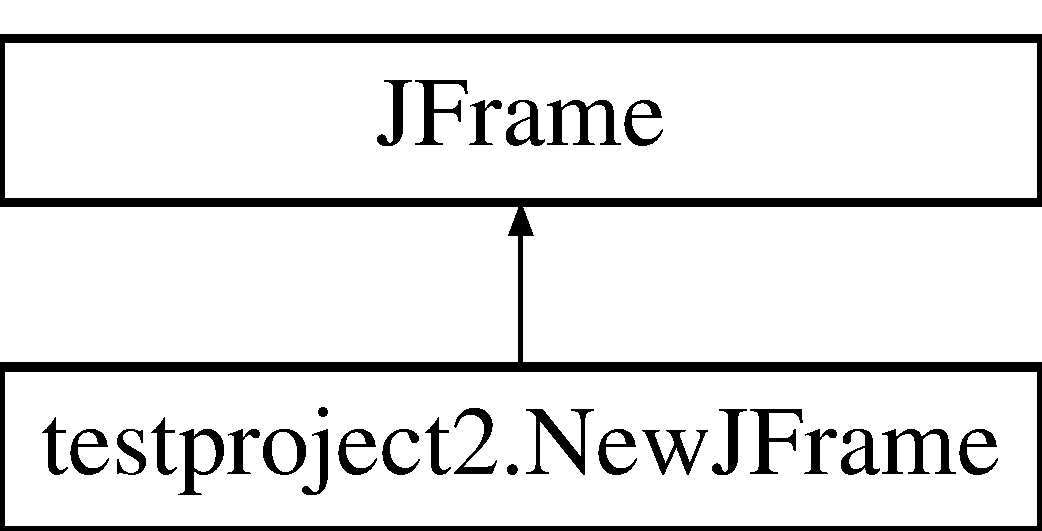
\includegraphics[height=2.000000cm]{classtestproject2_1_1NewJFrame}
\end{center}
\end{figure}
\subsection*{Classes}
\begin{DoxyCompactItemize}
\item 
class {\bfseries Auto\-Fill\-Listener}
\item 
class {\bfseries Auto\-Fill\-Popup}
\item 
class {\bfseries j\-Text\-Area\-Keyboard\-Listener}
\end{DoxyCompactItemize}
\subsection*{Public Member Functions}
\begin{DoxyCompactItemize}
\item 
\hyperlink{classtestproject2_1_1NewJFrame_a1099755dc9b88a85dea21532fef90fb9}{New\-J\-Frame} ()
\end{DoxyCompactItemize}
\subsection*{Static Public Member Functions}
\begin{DoxyCompactItemize}
\item 
static void \hyperlink{classtestproject2_1_1NewJFrame_aebffd7abd3d6ed0a4307c36bb2f20fa5}{main} (String args\mbox{[}$\,$\mbox{]})
\end{DoxyCompactItemize}


\subsection{Detailed Description}
\begin{DoxyAuthor}{Author}
loganludington 
\end{DoxyAuthor}


\subsection{Constructor \& Destructor Documentation}
\hypertarget{classtestproject2_1_1NewJFrame_a1099755dc9b88a85dea21532fef90fb9}{\index{testproject2\-::\-New\-J\-Frame@{testproject2\-::\-New\-J\-Frame}!New\-J\-Frame@{New\-J\-Frame}}
\index{New\-J\-Frame@{New\-J\-Frame}!testproject2::NewJFrame@{testproject2\-::\-New\-J\-Frame}}
\subsubsection[{New\-J\-Frame}]{\setlength{\rightskip}{0pt plus 5cm}testproject2.\-New\-J\-Frame.\-New\-J\-Frame (
\begin{DoxyParamCaption}
{}
\end{DoxyParamCaption}
)}}\label{classtestproject2_1_1NewJFrame_a1099755dc9b88a85dea21532fef90fb9}
Creates new form \hyperlink{classtestproject2_1_1NewJFrame}{New\-J\-Frame} 

\subsection{Member Function Documentation}
\hypertarget{classtestproject2_1_1NewJFrame_aebffd7abd3d6ed0a4307c36bb2f20fa5}{\index{testproject2\-::\-New\-J\-Frame@{testproject2\-::\-New\-J\-Frame}!main@{main}}
\index{main@{main}!testproject2::NewJFrame@{testproject2\-::\-New\-J\-Frame}}
\subsubsection[{main}]{\setlength{\rightskip}{0pt plus 5cm}static void testproject2.\-New\-J\-Frame.\-main (
\begin{DoxyParamCaption}
\item[{String}]{args\mbox{[}$\,$\mbox{]}}
\end{DoxyParamCaption}
)\hspace{0.3cm}{\ttfamily [static]}}}\label{classtestproject2_1_1NewJFrame_aebffd7abd3d6ed0a4307c36bb2f20fa5}

\begin{DoxyParams}{Parameters}
{\em args} & the command line arguments \\
\hline
\end{DoxyParams}


The documentation for this class was generated from the following file\-:\begin{DoxyCompactItemize}
\item 
branches/\-Testing\-Branch/\-Auto\-Fill\-Testing/src/testproject2/New\-J\-Frame.\-java\end{DoxyCompactItemize}

\hypertarget{classCASUAL_1_1archiving_1_1Odin}{\section{C\-A\-S\-U\-A\-L.\-archiving.\-Odin Class Reference}
\label{classCASUAL_1_1archiving_1_1Odin}\index{C\-A\-S\-U\-A\-L.\-archiving.\-Odin@{C\-A\-S\-U\-A\-L.\-archiving.\-Odin}}
}
\subsection*{Public Member Functions}
\begin{DoxyCompactItemize}
\item 
\hyperlink{classCASUAL_1_1archiving_1_1Odin_a0b866241e776314cf2f179795c4303c4}{Odin} (String heimdall\-Location)
\item 
\hypertarget{classCASUAL_1_1archiving_1_1Odin_a8d7f4bfb02dd6b023e9322270e89013c}{void {\bfseries reset} ()}\label{classCASUAL_1_1archiving_1_1Odin_a8d7f4bfb02dd6b023e9322270e89013c}

\item 
\hypertarget{classCASUAL_1_1archiving_1_1Odin_a0e92a86a4b6daf858e78f65d431bb226}{String\mbox{[}$\,$\mbox{]} {\bfseries get\-Odin\-Command} ()  throws File\-Not\-Found\-Exception, File\-Not\-Found\-Exception, Corrupt\-Odin\-File\-Exception }\label{classCASUAL_1_1archiving_1_1Odin_a0e92a86a4b6daf858e78f65d431bb226}

\item 
\hypertarget{classCASUAL_1_1archiving_1_1Odin_aef77b9a893f1faf7b57de25102621d03}{String\mbox{[}$\,$\mbox{]} {\bfseries get\-Flash\-Files\-Command} (File pit\-File, File\mbox{[}$\,$\mbox{]} files\-To\-Flash)  throws File\-Not\-Found\-Exception }\label{classCASUAL_1_1archiving_1_1Odin_aef77b9a893f1faf7b57de25102621d03}

\item 
\hypertarget{classCASUAL_1_1archiving_1_1Odin_ad628882606935f87692fe1fa10768a75}{String\mbox{[}$\,$\mbox{]} {\bfseries add\-Flash\-Files} (String\mbox{[}$\,$\mbox{]} Existing\-Command, File pit\-File, File\mbox{[}$\,$\mbox{]} files\-To\-Flash)  throws File\-Not\-Found\-Exception }\label{classCASUAL_1_1archiving_1_1Odin_ad628882606935f87692fe1fa10768a75}

\item 
\hypertarget{classCASUAL_1_1archiving_1_1Odin_ace41339836b3370f6d654a5d8752f658}{String\mbox{[}$\,$\mbox{]} {\bfseries add\-Repartition\-Command} (String\mbox{[}$\,$\mbox{]} Existing\-Command, File pit\-File)  throws File\-Not\-Found\-Exception }\label{classCASUAL_1_1archiving_1_1Odin_ace41339836b3370f6d654a5d8752f658}

\end{DoxyCompactItemize}
\subsection*{Public Attributes}
\begin{DoxyCompactItemize}
\item 
\hypertarget{classCASUAL_1_1archiving_1_1Odin_a2faa96ef3a5e321aebd74c714b7b427a}{boolean {\bfseries auto\-Reboot} = false}\label{classCASUAL_1_1archiving_1_1Odin_a2faa96ef3a5e321aebd74c714b7b427a}

\item 
\hypertarget{classCASUAL_1_1archiving_1_1Odin_ac9e05db747e8fc4085f5b947f388cec3}{boolean {\bfseries repartition} = false}\label{classCASUAL_1_1archiving_1_1Odin_ac9e05db747e8fc4085f5b947f388cec3}

\item 
\hypertarget{classCASUAL_1_1archiving_1_1Odin_a24ebdd39483395d4dbc36a39fdce64ce}{boolean {\bfseries flash\-Pit} = false}\label{classCASUAL_1_1archiving_1_1Odin_a24ebdd39483395d4dbc36a39fdce64ce}

\item 
\hypertarget{classCASUAL_1_1archiving_1_1Odin_a0175e05530541f1540db0a372a6fd1be}{File {\bfseries pit} = null}\label{classCASUAL_1_1archiving_1_1Odin_a0175e05530541f1540db0a372a6fd1be}

\item 
\hypertarget{classCASUAL_1_1archiving_1_1Odin_ab9a6d53365b4b04a35f7e3e5d92ba9cd}{boolean {\bfseries flash\-Bootloader} = false}\label{classCASUAL_1_1archiving_1_1Odin_ab9a6d53365b4b04a35f7e3e5d92ba9cd}

\item 
\hypertarget{classCASUAL_1_1archiving_1_1Odin_aeb3053624a23c6388290a0ba1414eb4d}{File {\bfseries bootloader} = null}\label{classCASUAL_1_1archiving_1_1Odin_aeb3053624a23c6388290a0ba1414eb4d}

\item 
\hypertarget{classCASUAL_1_1archiving_1_1Odin_a293d689851526a4284c3db4583d2d66a}{boolean {\bfseries flash\-Pda} = false}\label{classCASUAL_1_1archiving_1_1Odin_a293d689851526a4284c3db4583d2d66a}

\item 
\hypertarget{classCASUAL_1_1archiving_1_1Odin_a7e8e5e8b57b9941b2cdbcaac2cf1e3f8}{File {\bfseries pda} = null}\label{classCASUAL_1_1archiving_1_1Odin_a7e8e5e8b57b9941b2cdbcaac2cf1e3f8}

\item 
\hypertarget{classCASUAL_1_1archiving_1_1Odin_a457a237b0e92db675ca6d8ead4e138f1}{boolean {\bfseries flash\-Phone} = false}\label{classCASUAL_1_1archiving_1_1Odin_a457a237b0e92db675ca6d8ead4e138f1}

\item 
\hypertarget{classCASUAL_1_1archiving_1_1Odin_a667a73f5890479d4ed2c25bb0a42f0dc}{File {\bfseries phone} = null}\label{classCASUAL_1_1archiving_1_1Odin_a667a73f5890479d4ed2c25bb0a42f0dc}

\item 
\hypertarget{classCASUAL_1_1archiving_1_1Odin_a83e1a15719249f650fee9adacfffced6}{boolean {\bfseries flash\-Csc} = false}\label{classCASUAL_1_1archiving_1_1Odin_a83e1a15719249f650fee9adacfffced6}

\item 
\hypertarget{classCASUAL_1_1archiving_1_1Odin_a82b4ba64c18dcdf38a698b024560cbc5}{File {\bfseries csc} = null}\label{classCASUAL_1_1archiving_1_1Odin_a82b4ba64c18dcdf38a698b024560cbc5}

\end{DoxyCompactItemize}


\subsection{Detailed Description}
\begin{DoxyAuthor}{Author}
adamoutler 
\end{DoxyAuthor}


\subsection{Constructor \& Destructor Documentation}
\hypertarget{classCASUAL_1_1archiving_1_1Odin_a0b866241e776314cf2f179795c4303c4}{\index{C\-A\-S\-U\-A\-L\-::archiving\-::\-Odin@{C\-A\-S\-U\-A\-L\-::archiving\-::\-Odin}!Odin@{Odin}}
\index{Odin@{Odin}!CASUAL::archiving::Odin@{C\-A\-S\-U\-A\-L\-::archiving\-::\-Odin}}
\subsubsection[{Odin}]{\setlength{\rightskip}{0pt plus 5cm}C\-A\-S\-U\-A\-L.\-archiving.\-Odin.\-Odin (
\begin{DoxyParamCaption}
\item[{String}]{heimdall\-Location}
\end{DoxyParamCaption}
)}}\label{classCASUAL_1_1archiving_1_1Odin_a0b866241e776314cf2f179795c4303c4}
Public constructor creates pit stream from pit file


\begin{DoxyParams}{Parameters}
{\em heimdall\-Location} & location to Heimdall binary \\
\hline
\end{DoxyParams}


The documentation for this class was generated from the following file\-:\begin{DoxyCompactItemize}
\item 
trunk/\-C\-A\-S\-U\-A\-Lcore/src/\-C\-A\-S\-U\-A\-L/archiving/Odin.\-java\end{DoxyCompactItemize}

\hypertarget{classCASUAL_1_1archiving_1_1OdinFile}{\section{C\-A\-S\-U\-A\-L.\-archiving.\-Odin\-File Class Reference}
\label{classCASUAL_1_1archiving_1_1OdinFile}\index{C\-A\-S\-U\-A\-L.\-archiving.\-Odin\-File@{C\-A\-S\-U\-A\-L.\-archiving.\-Odin\-File}}
}
\subsection*{Public Member Functions}
\begin{DoxyCompactItemize}
\item 
\hyperlink{classCASUAL_1_1archiving_1_1OdinFile_a89c41c4bc7f61f112fc06b61bd8dda88}{Odin\-File} (File odin\-File)  throws File\-Not\-Found\-Exception, I\-O\-Exception, No\-Such\-Algorithm\-Exception, Corrupt\-Odin\-File\-Exception, Archive\-Exception 
\item 
\hyperlink{classCASUAL_1_1archiving_1_1OdinFile_a68fe33b8b91c48ce0bf31d821b666e0b}{Odin\-File} (String odin\-File)  throws File\-Not\-Found\-Exception, I\-O\-Exception, No\-Such\-Algorithm\-Exception, Corrupt\-Odin\-File\-Exception, Archive\-Exception 
\item 
File\mbox{[}$\,$\mbox{]} \hyperlink{classCASUAL_1_1archiving_1_1OdinFile_a1c6900921a7fedd0ed75c9003e8b64b0}{extract\-Odin\-Contents} (String output\-Dir)  throws I\-O\-Exception, Archive\-Exception, No\-Such\-Algorithm\-Exception 
\end{DoxyCompactItemize}


\subsection{Detailed Description}
\begin{DoxyAuthor}{Author}
adamoutler 
\end{DoxyAuthor}


\subsection{Constructor \& Destructor Documentation}
\hypertarget{classCASUAL_1_1archiving_1_1OdinFile_a89c41c4bc7f61f112fc06b61bd8dda88}{\index{C\-A\-S\-U\-A\-L\-::archiving\-::\-Odin\-File@{C\-A\-S\-U\-A\-L\-::archiving\-::\-Odin\-File}!Odin\-File@{Odin\-File}}
\index{Odin\-File@{Odin\-File}!CASUAL::archiving::OdinFile@{C\-A\-S\-U\-A\-L\-::archiving\-::\-Odin\-File}}
\subsubsection[{Odin\-File}]{\setlength{\rightskip}{0pt plus 5cm}C\-A\-S\-U\-A\-L.\-archiving.\-Odin\-File.\-Odin\-File (
\begin{DoxyParamCaption}
\item[{File}]{odin\-File}
\end{DoxyParamCaption}
) throws File\-Not\-Found\-Exception, I\-O\-Exception, No\-Such\-Algorithm\-Exception, {\bf Corrupt\-Odin\-File\-Exception}, Archive\-Exception}}\label{classCASUAL_1_1archiving_1_1OdinFile_a89c41c4bc7f61f112fc06b61bd8dda88}
Opens an \hyperlink{classCASUAL_1_1archiving_1_1Odin}{Odin} file and verifies M\-D5sum 
\begin{DoxyParams}{Parameters}
{\em odin\-File} & file to be opened and verified \\
\hline
\end{DoxyParams}

\begin{DoxyExceptions}{Exceptions}
{\em \hyperlink{classCASUAL_1_1archiving_1_1CorruptOdinFileException}{Corrupt\-Odin\-File\-Exception}} & \hyperlink{classCASUAL_1_1archiving_1_1Odin}{Odin} checks did not pass \\
\hline
{\em File\-Not\-Found\-Exception} & \\
\hline
{\em I\-O\-Exception} & \\
\hline
{\em No\-Such\-Algorithm\-Exception} & \\
\hline
{\em org.\-apache.\-commons.\-compress.\-archivers.\-Archive\-Exception} & \\
\hline
\end{DoxyExceptions}
\hypertarget{classCASUAL_1_1archiving_1_1OdinFile_a68fe33b8b91c48ce0bf31d821b666e0b}{\index{C\-A\-S\-U\-A\-L\-::archiving\-::\-Odin\-File@{C\-A\-S\-U\-A\-L\-::archiving\-::\-Odin\-File}!Odin\-File@{Odin\-File}}
\index{Odin\-File@{Odin\-File}!CASUAL::archiving::OdinFile@{C\-A\-S\-U\-A\-L\-::archiving\-::\-Odin\-File}}
\subsubsection[{Odin\-File}]{\setlength{\rightskip}{0pt plus 5cm}C\-A\-S\-U\-A\-L.\-archiving.\-Odin\-File.\-Odin\-File (
\begin{DoxyParamCaption}
\item[{String}]{odin\-File}
\end{DoxyParamCaption}
) throws File\-Not\-Found\-Exception, I\-O\-Exception, No\-Such\-Algorithm\-Exception, {\bf Corrupt\-Odin\-File\-Exception}, Archive\-Exception}}\label{classCASUAL_1_1archiving_1_1OdinFile_a68fe33b8b91c48ce0bf31d821b666e0b}
Opens an \hyperlink{classCASUAL_1_1archiving_1_1Odin}{Odin} file and verifies M\-D5sum 
\begin{DoxyParams}{Parameters}
{\em odin\-File} & file to be opened and verified \\
\hline
\end{DoxyParams}

\begin{DoxyExceptions}{Exceptions}
{\em \hyperlink{classCASUAL_1_1archiving_1_1CorruptOdinFileException}{Corrupt\-Odin\-File\-Exception}} & \hyperlink{classCASUAL_1_1archiving_1_1Odin}{Odin} checks did not pass \\
\hline
{\em File\-Not\-Found\-Exception} & \\
\hline
{\em I\-O\-Exception} & \\
\hline
{\em No\-Such\-Algorithm\-Exception} & \\
\hline
{\em org.\-apache.\-commons.\-compress.\-archivers.\-Archive\-Exception} & \\
\hline
\end{DoxyExceptions}


\subsection{Member Function Documentation}
\hypertarget{classCASUAL_1_1archiving_1_1OdinFile_a1c6900921a7fedd0ed75c9003e8b64b0}{\index{C\-A\-S\-U\-A\-L\-::archiving\-::\-Odin\-File@{C\-A\-S\-U\-A\-L\-::archiving\-::\-Odin\-File}!extract\-Odin\-Contents@{extract\-Odin\-Contents}}
\index{extract\-Odin\-Contents@{extract\-Odin\-Contents}!CASUAL::archiving::OdinFile@{C\-A\-S\-U\-A\-L\-::archiving\-::\-Odin\-File}}
\subsubsection[{extract\-Odin\-Contents}]{\setlength{\rightskip}{0pt plus 5cm}File \mbox{[}$\,$\mbox{]} C\-A\-S\-U\-A\-L.\-archiving.\-Odin\-File.\-extract\-Odin\-Contents (
\begin{DoxyParamCaption}
\item[{String}]{output\-Dir}
\end{DoxyParamCaption}
) throws I\-O\-Exception, Archive\-Exception, No\-Such\-Algorithm\-Exception}}\label{classCASUAL_1_1archiving_1_1OdinFile_a1c6900921a7fedd0ed75c9003e8b64b0}
Extracts \hyperlink{classCASUAL_1_1archiving_1_1Odin}{Odin} contents to output\-Dir 
\begin{DoxyParams}{Parameters}
{\em output\-Dir} & temp folder \\
\hline
\end{DoxyParams}
\begin{DoxyReturn}{Returns}
an array of files extracted from \hyperlink{classCASUAL_1_1archiving_1_1Odin}{Odin} Package 
\end{DoxyReturn}

\begin{DoxyExceptions}{Exceptions}
{\em I\-O\-Exception} & \\
\hline
{\em Archive\-Exception} & \\
\hline
{\em No\-Such\-Algorithm\-Exception} & \\
\hline
\end{DoxyExceptions}


The documentation for this class was generated from the following file\-:\begin{DoxyCompactItemize}
\item 
trunk/\-C\-A\-S\-U\-A\-Lcore/src/\-C\-A\-S\-U\-A\-L/archiving/Odin\-File.\-java\end{DoxyCompactItemize}

\hypertarget{classCASUAL_1_1archiving_1_1OdinFileTest}{\section{C\-A\-S\-U\-A\-L.\-archiving.\-Odin\-File\-Test Class Reference}
\label{classCASUAL_1_1archiving_1_1OdinFileTest}\index{C\-A\-S\-U\-A\-L.\-archiving.\-Odin\-File\-Test@{C\-A\-S\-U\-A\-L.\-archiving.\-Odin\-File\-Test}}
}
\subsection*{Public Member Functions}
\begin{DoxyCompactItemize}
\item 
\hypertarget{classCASUAL_1_1archiving_1_1OdinFileTest_a334d704de50ba1014977e0b4a3112665}{void {\bfseries set\-Up} ()}\label{classCASUAL_1_1archiving_1_1OdinFileTest_a334d704de50ba1014977e0b4a3112665}

\item 
\hypertarget{classCASUAL_1_1archiving_1_1OdinFileTest_a1fbededbb0dc328c74d57c6665df2be4}{void {\bfseries tear\-Down} ()}\label{classCASUAL_1_1archiving_1_1OdinFileTest_a1fbededbb0dc328c74d57c6665df2be4}

\item 
void \hyperlink{classCASUAL_1_1archiving_1_1OdinFileTest_a65ccebb5135d4a731c4db6b1fa30e2b7}{test\-Open} ()  throws Exception 
\end{DoxyCompactItemize}
\subsection*{Static Public Member Functions}
\begin{DoxyCompactItemize}
\item 
\hypertarget{classCASUAL_1_1archiving_1_1OdinFileTest_a4f348dec88c1ed7c45682b6c1c878243}{static void {\bfseries set\-Up\-Class} ()}\label{classCASUAL_1_1archiving_1_1OdinFileTest_a4f348dec88c1ed7c45682b6c1c878243}

\item 
\hypertarget{classCASUAL_1_1archiving_1_1OdinFileTest_a495a53b6e728e43afaf45612c0ece1cd}{static void {\bfseries tear\-Down\-Class} ()}\label{classCASUAL_1_1archiving_1_1OdinFileTest_a495a53b6e728e43afaf45612c0ece1cd}

\end{DoxyCompactItemize}


\subsection{Detailed Description}
\begin{DoxyAuthor}{Author}
adamoutler 
\end{DoxyAuthor}


\subsection{Member Function Documentation}
\hypertarget{classCASUAL_1_1archiving_1_1OdinFileTest_a65ccebb5135d4a731c4db6b1fa30e2b7}{\index{C\-A\-S\-U\-A\-L\-::archiving\-::\-Odin\-File\-Test@{C\-A\-S\-U\-A\-L\-::archiving\-::\-Odin\-File\-Test}!test\-Open@{test\-Open}}
\index{test\-Open@{test\-Open}!CASUAL::archiving::OdinFileTest@{C\-A\-S\-U\-A\-L\-::archiving\-::\-Odin\-File\-Test}}
\subsubsection[{test\-Open}]{\setlength{\rightskip}{0pt plus 5cm}void C\-A\-S\-U\-A\-L.\-archiving.\-Odin\-File\-Test.\-test\-Open (
\begin{DoxyParamCaption}
{}
\end{DoxyParamCaption}
) throws Exception}}\label{classCASUAL_1_1archiving_1_1OdinFileTest_a65ccebb5135d4a731c4db6b1fa30e2b7}
Test of open method, of class Odin\-Decompressor.


\begin{DoxyExceptions}{Exceptions}
{\em java.\-lang.\-Exception} & \\
\hline
\end{DoxyExceptions}


The documentation for this class was generated from the following file\-:\begin{DoxyCompactItemize}
\item 
trunk/\-C\-A\-S\-U\-A\-Lcore/test/\-C\-A\-S\-U\-A\-L/archiving/Odin\-File\-Test.\-java\end{DoxyCompactItemize}

\hypertarget{classCASUAL_1_1archiving_1_1OdinTest}{\section{C\-A\-S\-U\-A\-L.\-archiving.\-Odin\-Test Class Reference}
\label{classCASUAL_1_1archiving_1_1OdinTest}\index{C\-A\-S\-U\-A\-L.\-archiving.\-Odin\-Test@{C\-A\-S\-U\-A\-L.\-archiving.\-Odin\-Test}}
}
\subsection*{Public Member Functions}
\begin{DoxyCompactItemize}
\item 
\hypertarget{classCASUAL_1_1archiving_1_1OdinTest_ad34fd1644e8066e376256efffe658484}{void {\bfseries set\-Up} ()}\label{classCASUAL_1_1archiving_1_1OdinTest_ad34fd1644e8066e376256efffe658484}

\item 
\hypertarget{classCASUAL_1_1archiving_1_1OdinTest_ac64874c4e16ed83cd449fd60920d39ad}{void {\bfseries tear\-Down} ()}\label{classCASUAL_1_1archiving_1_1OdinTest_ac64874c4e16ed83cd449fd60920d39ad}

\item 
void \hyperlink{classCASUAL_1_1archiving_1_1OdinTest_aedccee3742d364c32e152b316a5502cd}{test\-Get\-Heimdall\-Command} ()  throws Exception 
\end{DoxyCompactItemize}
\subsection*{Static Public Member Functions}
\begin{DoxyCompactItemize}
\item 
\hypertarget{classCASUAL_1_1archiving_1_1OdinTest_a8cd2b267a73851fb26aaca8173f52abd}{static void {\bfseries set\-Up\-Class} ()  throws Exception }\label{classCASUAL_1_1archiving_1_1OdinTest_a8cd2b267a73851fb26aaca8173f52abd}

\item 
\hypertarget{classCASUAL_1_1archiving_1_1OdinTest_a5b896696c51151707e62c81cf650f32e}{static void {\bfseries tear\-Down\-Class} ()}\label{classCASUAL_1_1archiving_1_1OdinTest_a5b896696c51151707e62c81cf650f32e}

\end{DoxyCompactItemize}


\subsection{Detailed Description}
\begin{DoxyAuthor}{Author}
adamoutler 
\end{DoxyAuthor}


\subsection{Member Function Documentation}
\hypertarget{classCASUAL_1_1archiving_1_1OdinTest_aedccee3742d364c32e152b316a5502cd}{\index{C\-A\-S\-U\-A\-L\-::archiving\-::\-Odin\-Test@{C\-A\-S\-U\-A\-L\-::archiving\-::\-Odin\-Test}!test\-Get\-Heimdall\-Command@{test\-Get\-Heimdall\-Command}}
\index{test\-Get\-Heimdall\-Command@{test\-Get\-Heimdall\-Command}!CASUAL::archiving::OdinTest@{C\-A\-S\-U\-A\-L\-::archiving\-::\-Odin\-Test}}
\subsubsection[{test\-Get\-Heimdall\-Command}]{\setlength{\rightskip}{0pt plus 5cm}void C\-A\-S\-U\-A\-L.\-archiving.\-Odin\-Test.\-test\-Get\-Heimdall\-Command (
\begin{DoxyParamCaption}
{}
\end{DoxyParamCaption}
) throws Exception}}\label{classCASUAL_1_1archiving_1_1OdinTest_aedccee3742d364c32e152b316a5502cd}
Test of get\-Heimdall\-Command method, of class Heimdall\-Formatter.


\begin{DoxyExceptions}{Exceptions}
{\em java.\-lang.\-Exception} & \\
\hline
\end{DoxyExceptions}


The documentation for this class was generated from the following file\-:\begin{DoxyCompactItemize}
\item 
trunk/\-C\-A\-S\-U\-A\-Lcore/test/\-C\-A\-S\-U\-A\-L/archiving/Odin\-Test.\-java\end{DoxyCompactItemize}

\hypertarget{enumdevicedetector_1_1msiexecInterface_1_1Operation}{\section{devicedetector.\-msiexec\-Interface.\-Operation Enum Reference}
\label{enumdevicedetector_1_1msiexecInterface_1_1Operation}\index{devicedetector.\-msiexec\-Interface.\-Operation@{devicedetector.\-msiexec\-Interface.\-Operation}}
}
\subsection*{Public Attributes}
\begin{DoxyCompactItemize}
\item 
\hypertarget{enumdevicedetector_1_1msiexecInterface_1_1Operation_af779693a31ca83040f50caf3c493c6ab}{{\bfseries I\-N\-S\-T\-A\-L\-L}}\label{enumdevicedetector_1_1msiexecInterface_1_1Operation_af779693a31ca83040f50caf3c493c6ab}

\item 
\hypertarget{enumdevicedetector_1_1msiexecInterface_1_1Operation_a56b8216ad7aed635ef00c62d7d4a29d3}{{\bfseries R\-E\-P\-A\-I\-R}}\label{enumdevicedetector_1_1msiexecInterface_1_1Operation_a56b8216ad7aed635ef00c62d7d4a29d3}

\item 
\hypertarget{enumdevicedetector_1_1msiexecInterface_1_1Operation_a2411632c1e472c33d6ee8a6b6e5863df}{{\bfseries U\-N\-I\-N\-S\-T\-A\-L\-L}}\label{enumdevicedetector_1_1msiexecInterface_1_1Operation_a2411632c1e472c33d6ee8a6b6e5863df}

\end{DoxyCompactItemize}


The documentation for this enum was generated from the following file\-:\begin{DoxyCompactItemize}
\item 
branches/\-Testing\-Branch/\-Device\-Detector/src/devicedetector/msiexec\-Interface.\-java\end{DoxyCompactItemize}

\hypertarget{classCASUAL_1_1OSTools}{\section{C\-A\-S\-U\-A\-L.\-O\-S\-Tools Class Reference}
\label{classCASUAL_1_1OSTools}\index{C\-A\-S\-U\-A\-L.\-O\-S\-Tools@{C\-A\-S\-U\-A\-L.\-O\-S\-Tools}}
}
\subsection*{Static Public Member Functions}
\begin{DoxyCompactItemize}
\item 
\hypertarget{classCASUAL_1_1OSTools_a0e56ffe8c5d4bb116822b580bc446f88}{static boolean {\bfseries is\-Mac} ()}\label{classCASUAL_1_1OSTools_a0e56ffe8c5d4bb116822b580bc446f88}

\item 
\hypertarget{classCASUAL_1_1OSTools_a8068ad9e8a1c65f19983881b0e0b24a1}{static boolean {\bfseries is64bit\-System} ()}\label{classCASUAL_1_1OSTools_a8068ad9e8a1c65f19983881b0e0b24a1}

\item 
\hypertarget{classCASUAL_1_1OSTools_aec6bfc5a30c3575087ed4f01fe097224}{static String {\bfseries check\-Linux\-Arch} ()}\label{classCASUAL_1_1OSTools_aec6bfc5a30c3575087ed4f01fe097224}

\item 
\hypertarget{classCASUAL_1_1OSTools_aba47c5eb8808b1068b08e95879dd3398}{static boolean {\bfseries is\-Windows64\-Arch} ()}\label{classCASUAL_1_1OSTools_aba47c5eb8808b1068b08e95879dd3398}

\item 
\hypertarget{classCASUAL_1_1OSTools_a30268489d47f25c2bf74fc081e2f059a}{static String {\bfseries O\-S\-Name} ()}\label{classCASUAL_1_1OSTools_a30268489d47f25c2bf74fc081e2f059a}

\item 
\hypertarget{classCASUAL_1_1OSTools_a41ba4fa3af5e04583de46598a9d39e73}{static boolean {\bfseries is\-Linux} ()}\label{classCASUAL_1_1OSTools_a41ba4fa3af5e04583de46598a9d39e73}

\item 
\hypertarget{classCASUAL_1_1OSTools_ab0171f3f220d9e3bdbf131e0f0546e00}{static boolean {\bfseries is\-Windows} ()}\label{classCASUAL_1_1OSTools_ab0171f3f220d9e3bdbf131e0f0546e00}

\end{DoxyCompactItemize}


\subsection{Detailed Description}
\begin{DoxyAuthor}{Author}
adam 
\end{DoxyAuthor}


The documentation for this class was generated from the following file\-:\begin{DoxyCompactItemize}
\item 
trunk/\-C\-A\-S\-U\-A\-Lcore/src/\-C\-A\-S\-U\-A\-L/O\-S\-Tools.\-java\end{DoxyCompactItemize}

\hypertarget{classCASPACkager_1_1PackagerMain}{\section{C\-A\-S\-P\-A\-Ckager.\-Packager\-Main Class Reference}
\label{classCASPACkager_1_1PackagerMain}\index{C\-A\-S\-P\-A\-Ckager.\-Packager\-Main@{C\-A\-S\-P\-A\-Ckager.\-Packager\-Main}}
}
\subsection*{Public Member Functions}
\begin{DoxyCompactItemize}
\item 
\hyperlink{classCASPACkager_1_1PackagerMain_a5feeab84510603114e4cd16af557183f}{Packager\-Main} ()
\item 
void \hyperlink{classCASPACkager_1_1PackagerMain_a4e8e02f802540050d3f1a074a9f4b411}{merge\-Caspac\-Casual} ()
\item 
void \hyperlink{classCASPACkager_1_1PackagerMain_a32df460e9180f81a54b7d7a3c38215cc}{merge\-Caspac\-Casual} (String caspac\-Loc)
\item 
void \hyperlink{classCASPACkager_1_1PackagerMain_ab3e1a27e66331e67b19ae4809480f46a}{merge\-Caspac\-Casual} (String caspac\-Loc, String output\-Dir)
\item 
String\mbox{[}$\,$\mbox{]} \hyperlink{classCASPACkager_1_1PackagerMain_afdf339fc0283b3cf6418de0e59732762}{get\-Caspac\-File\-List} ()
\item 
String\mbox{[}$\,$\mbox{]} \hyperlink{classCASPACkager_1_1PackagerMain_ae9bf358f30038bfb45e7de7bf2c3c0a6}{get\-Caspac\-File\-List} (String caspac\-Loc)
\item 
String\mbox{[}$\,$\mbox{]} \hyperlink{classCASPACkager_1_1PackagerMain_aa741699d712b8b9cecb5a6782838413d}{get\-Caspac\-File\-List} (File caspac)
\item 
Input\-Stream \hyperlink{classCASPACkager_1_1PackagerMain_aac9b44ae631f522eb53efce869f3a5c5}{repack\-Entry} (Zip\-Entry entry, String working)
\end{DoxyCompactItemize}
\subsection*{Static Public Member Functions}
\begin{DoxyCompactItemize}
\item 
static void \hyperlink{classCASPACkager_1_1PackagerMain_ab65464d17a9ed1557137ca0fc128f320}{main} (final String\mbox{[}$\,$\mbox{]} args)
\end{DoxyCompactItemize}
\subsection*{Static Protected Attributes}
\begin{DoxyCompactItemize}
\item 
static String \hyperlink{classCASPACkager_1_1PackagerMain_a0095242e26294a46bcb44dde15d36c38}{user\-Output\-Dir} = \char`\"{}\char`\"{}
\end{DoxyCompactItemize}


\subsection{Detailed Description}


 \hyperlink{classCASPACkager_1_1PackagerMain}{Packager\-Main} packages a C\-A\-S\-P\-A\-C into a \hyperlink{namespaceCASUAL}{C\-A\-S\-U\-A\-L} and provides a method of modifying a C\-A\-S\-P\-A\-C on the fly as a part of packaging. \begin{DoxyAuthor}{Author}
Jeremy Loper \href{mailto:jrloper@gmail.com}{\tt jrloper@gmail.\-com} 

Logan Ludington \href{mailto:loglud@logatech.org}{\tt loglud@logatech.\-org} 

 
\end{DoxyAuthor}


\subsection{Constructor \& Destructor Documentation}
\hypertarget{classCASPACkager_1_1PackagerMain_a5feeab84510603114e4cd16af557183f}{\index{C\-A\-S\-P\-A\-Ckager\-::\-Packager\-Main@{C\-A\-S\-P\-A\-Ckager\-::\-Packager\-Main}!Packager\-Main@{Packager\-Main}}
\index{Packager\-Main@{Packager\-Main}!CASPACkager::PackagerMain@{C\-A\-S\-P\-A\-Ckager\-::\-Packager\-Main}}
\subsubsection[{Packager\-Main}]{\setlength{\rightskip}{0pt plus 5cm}C\-A\-S\-P\-A\-Ckager.\-Packager\-Main.\-Packager\-Main (
\begin{DoxyParamCaption}
{}
\end{DoxyParamCaption}
)}}\label{classCASPACkager_1_1PackagerMain_a5feeab84510603114e4cd16af557183f}
instantiates Packager 

\subsection{Member Function Documentation}
\hypertarget{classCASPACkager_1_1PackagerMain_afdf339fc0283b3cf6418de0e59732762}{\index{C\-A\-S\-P\-A\-Ckager\-::\-Packager\-Main@{C\-A\-S\-P\-A\-Ckager\-::\-Packager\-Main}!get\-Caspac\-File\-List@{get\-Caspac\-File\-List}}
\index{get\-Caspac\-File\-List@{get\-Caspac\-File\-List}!CASPACkager::PackagerMain@{C\-A\-S\-P\-A\-Ckager\-::\-Packager\-Main}}
\subsubsection[{get\-Caspac\-File\-List}]{\setlength{\rightskip}{0pt plus 5cm}String \mbox{[}$\,$\mbox{]} C\-A\-S\-P\-A\-Ckager.\-Packager\-Main.\-get\-Caspac\-File\-List (
\begin{DoxyParamCaption}
{}
\end{DoxyParamCaption}
)}}\label{classCASPACkager_1_1PackagerMain_afdf339fc0283b3cf6418de0e59732762}
gets the list of files in the C\-A\-S\-P\-A\-C.

\begin{DoxyReturn}{Returns}
path to files 
\end{DoxyReturn}
\hypertarget{classCASPACkager_1_1PackagerMain_ae9bf358f30038bfb45e7de7bf2c3c0a6}{\index{C\-A\-S\-P\-A\-Ckager\-::\-Packager\-Main@{C\-A\-S\-P\-A\-Ckager\-::\-Packager\-Main}!get\-Caspac\-File\-List@{get\-Caspac\-File\-List}}
\index{get\-Caspac\-File\-List@{get\-Caspac\-File\-List}!CASPACkager::PackagerMain@{C\-A\-S\-P\-A\-Ckager\-::\-Packager\-Main}}
\subsubsection[{get\-Caspac\-File\-List}]{\setlength{\rightskip}{0pt plus 5cm}String \mbox{[}$\,$\mbox{]} C\-A\-S\-P\-A\-Ckager.\-Packager\-Main.\-get\-Caspac\-File\-List (
\begin{DoxyParamCaption}
\item[{String}]{caspac\-Loc}
\end{DoxyParamCaption}
)}}\label{classCASPACkager_1_1PackagerMain_ae9bf358f30038bfb45e7de7bf2c3c0a6}
gets the list of files in the C\-A\-S\-P\-A\-C.


\begin{DoxyParams}{Parameters}
{\em caspac\-Loc} & path to\-C\-A\-S\-P\-A\-C \\
\hline
\end{DoxyParams}
\begin{DoxyReturn}{Returns}
path to files 
\end{DoxyReturn}
\hypertarget{classCASPACkager_1_1PackagerMain_aa741699d712b8b9cecb5a6782838413d}{\index{C\-A\-S\-P\-A\-Ckager\-::\-Packager\-Main@{C\-A\-S\-P\-A\-Ckager\-::\-Packager\-Main}!get\-Caspac\-File\-List@{get\-Caspac\-File\-List}}
\index{get\-Caspac\-File\-List@{get\-Caspac\-File\-List}!CASPACkager::PackagerMain@{C\-A\-S\-P\-A\-Ckager\-::\-Packager\-Main}}
\subsubsection[{get\-Caspac\-File\-List}]{\setlength{\rightskip}{0pt plus 5cm}String \mbox{[}$\,$\mbox{]} C\-A\-S\-P\-A\-Ckager.\-Packager\-Main.\-get\-Caspac\-File\-List (
\begin{DoxyParamCaption}
\item[{File}]{caspac}
\end{DoxyParamCaption}
)}}\label{classCASPACkager_1_1PackagerMain_aa741699d712b8b9cecb5a6782838413d}
gets the list of files in the C\-A\-S\-P\-A\-C. caspac file object representing the C\-A\-S\-P\-A\-C


\begin{DoxyParams}{Parameters}
{\em caspac} & to be examined \\
\hline
\end{DoxyParams}
\begin{DoxyReturn}{Returns}
path to files 
\end{DoxyReturn}
\hypertarget{classCASPACkager_1_1PackagerMain_ab65464d17a9ed1557137ca0fc128f320}{\index{C\-A\-S\-P\-A\-Ckager\-::\-Packager\-Main@{C\-A\-S\-P\-A\-Ckager\-::\-Packager\-Main}!main@{main}}
\index{main@{main}!CASPACkager::PackagerMain@{C\-A\-S\-P\-A\-Ckager\-::\-Packager\-Main}}
\subsubsection[{main}]{\setlength{\rightskip}{0pt plus 5cm}static void C\-A\-S\-P\-A\-Ckager.\-Packager\-Main.\-main (
\begin{DoxyParamCaption}
\item[{final String\mbox{[}$\,$\mbox{]}}]{args}
\end{DoxyParamCaption}
)\hspace{0.3cm}{\ttfamily [static]}}}\label{classCASPACkager_1_1PackagerMain_ab65464d17a9ed1557137ca0fc128f320}
Packages a C\-A\-S\-P\-A\-C into a \hyperlink{namespaceCASUAL}{C\-A\-S\-U\-A\-L}.


\begin{DoxyParams}{Parameters}
{\em args} & input from command line where args can be the following\-: --C\-A\-S\-P\-A\-C $|$$|$ -\/c \char`\"{}/path\-\_\-to/\-C\-A\-S\-P\-A\-C.$\ast$\char`\"{} specifies the path to the C\-A\-S\-P\-A\-C eg \char`\"{}-\/-\/\-C\-A\-S\-P\-A\-C C\-:/mycaspac.\-zip\char`\"{}. --output $|$$|$ -\/o \char`\"{}/path\-\_\-to/\-Output\-C\-A\-S\-U\-A\-L.\-jar\char`\"{} specifies an output file name. --type $|$$|$ -\/t \char`\"{}words to be appended before
jar\char`\"{} appends words to the end of the filename eg \char`\"{}-\/-\/type nightly\char`\"{} results\-: C\-A\-S\-P\-A\-C-\/\-C\-A\-S\-U\-A\-Lr327-\/nightly.\-jar.\\
\hline
\end{DoxyParams}
--fullauto $|$$|$ -\/f \char`\"{}/path\-\_\-to\-\_\-\-C\-A\-S\-P\-A\-C\-\_\-\-Folder/\char`\"{} Creates a folder in the specified fullauto path called \char`\"{}\-C\-A\-S\-U\-A\-L\char`\"{}. Generates new C\-A\-S\-U\-A\-L.\-jar files based upon each C\-A\-S\-P\-A\-C name in the full auto folder eg \char`\"{}-\/-\/fullauto
/path/to/folder\char`\"{} will process all C\-A\-S\-P\-A\-Cs in the folder and output to /path/to/folder/\-C\-A\-S\-U\-A\-L/. May be used with --type. cannot be used with --output or --C\-A\-S\-P\-A\-C arguments. \hypertarget{classCASPACkager_1_1PackagerMain_a4e8e02f802540050d3f1a074a9f4b411}{\index{C\-A\-S\-P\-A\-Ckager\-::\-Packager\-Main@{C\-A\-S\-P\-A\-Ckager\-::\-Packager\-Main}!merge\-Caspac\-Casual@{merge\-Caspac\-Casual}}
\index{merge\-Caspac\-Casual@{merge\-Caspac\-Casual}!CASPACkager::PackagerMain@{C\-A\-S\-P\-A\-Ckager\-::\-Packager\-Main}}
\subsubsection[{merge\-Caspac\-Casual}]{\setlength{\rightskip}{0pt plus 5cm}void C\-A\-S\-P\-A\-Ckager.\-Packager\-Main.\-merge\-Caspac\-Casual (
\begin{DoxyParamCaption}
{}
\end{DoxyParamCaption}
)}}\label{classCASPACkager_1_1PackagerMain_a4e8e02f802540050d3f1a074a9f4b411}
Merges the specified Caspac with the included \hyperlink{namespaceCASUAL}{C\-A\-S\-U\-A\-L}. \hypertarget{classCASPACkager_1_1PackagerMain_a32df460e9180f81a54b7d7a3c38215cc}{\index{C\-A\-S\-P\-A\-Ckager\-::\-Packager\-Main@{C\-A\-S\-P\-A\-Ckager\-::\-Packager\-Main}!merge\-Caspac\-Casual@{merge\-Caspac\-Casual}}
\index{merge\-Caspac\-Casual@{merge\-Caspac\-Casual}!CASPACkager::PackagerMain@{C\-A\-S\-P\-A\-Ckager\-::\-Packager\-Main}}
\subsubsection[{merge\-Caspac\-Casual}]{\setlength{\rightskip}{0pt plus 5cm}void C\-A\-S\-P\-A\-Ckager.\-Packager\-Main.\-merge\-Caspac\-Casual (
\begin{DoxyParamCaption}
\item[{String}]{caspac\-Loc}
\end{DoxyParamCaption}
)}}\label{classCASPACkager_1_1PackagerMain_a32df460e9180f81a54b7d7a3c38215cc}
Merges the specified Caspac with the included \hyperlink{namespaceCASUAL}{C\-A\-S\-U\-A\-L}.


\begin{DoxyParams}{Parameters}
{\em caspac\-Loc} & location to caspac \\
\hline
\end{DoxyParams}
\hypertarget{classCASPACkager_1_1PackagerMain_ab3e1a27e66331e67b19ae4809480f46a}{\index{C\-A\-S\-P\-A\-Ckager\-::\-Packager\-Main@{C\-A\-S\-P\-A\-Ckager\-::\-Packager\-Main}!merge\-Caspac\-Casual@{merge\-Caspac\-Casual}}
\index{merge\-Caspac\-Casual@{merge\-Caspac\-Casual}!CASPACkager::PackagerMain@{C\-A\-S\-P\-A\-Ckager\-::\-Packager\-Main}}
\subsubsection[{merge\-Caspac\-Casual}]{\setlength{\rightskip}{0pt plus 5cm}void C\-A\-S\-P\-A\-Ckager.\-Packager\-Main.\-merge\-Caspac\-Casual (
\begin{DoxyParamCaption}
\item[{String}]{caspac\-Loc, }
\item[{String}]{output\-Dir}
\end{DoxyParamCaption}
)}}\label{classCASPACkager_1_1PackagerMain_ab3e1a27e66331e67b19ae4809480f46a}
Merges the specified Caspac with the included \hyperlink{namespaceCASUAL}{C\-A\-S\-U\-A\-L}.


\begin{DoxyParams}{Parameters}
{\em caspac\-Loc} & location to caspac \\
\hline
{\em output\-Dir} & folder to output the \hyperlink{namespaceCASUAL}{C\-A\-S\-U\-A\-L} \\
\hline
\end{DoxyParams}
\hypertarget{classCASPACkager_1_1PackagerMain_aac9b44ae631f522eb53efce869f3a5c5}{\index{C\-A\-S\-P\-A\-Ckager\-::\-Packager\-Main@{C\-A\-S\-P\-A\-Ckager\-::\-Packager\-Main}!repack\-Entry@{repack\-Entry}}
\index{repack\-Entry@{repack\-Entry}!CASPACkager::PackagerMain@{C\-A\-S\-P\-A\-Ckager\-::\-Packager\-Main}}
\subsubsection[{repack\-Entry}]{\setlength{\rightskip}{0pt plus 5cm}Input\-Stream C\-A\-S\-P\-A\-Ckager.\-Packager\-Main.\-repack\-Entry (
\begin{DoxyParamCaption}
\item[{Zip\-Entry}]{entry, }
\item[{String}]{working}
\end{DoxyParamCaption}
)}}\label{classCASPACkager_1_1PackagerMain_aac9b44ae631f522eb53efce869f3a5c5}
adds a folder to the zip stream


\begin{DoxyParams}{Parameters}
{\em entry} & location to begin with \\
\hline
{\em working} & folder to compress \\
\hline
\end{DoxyParams}
\begin{DoxyReturn}{Returns}
inputstream representing the zip entry 
\end{DoxyReturn}


\subsection{Member Data Documentation}
\hypertarget{classCASPACkager_1_1PackagerMain_a0095242e26294a46bcb44dde15d36c38}{\index{C\-A\-S\-P\-A\-Ckager\-::\-Packager\-Main@{C\-A\-S\-P\-A\-Ckager\-::\-Packager\-Main}!user\-Output\-Dir@{user\-Output\-Dir}}
\index{user\-Output\-Dir@{user\-Output\-Dir}!CASPACkager::PackagerMain@{C\-A\-S\-P\-A\-Ckager\-::\-Packager\-Main}}
\subsubsection[{user\-Output\-Dir}]{\setlength{\rightskip}{0pt plus 5cm}String C\-A\-S\-P\-A\-Ckager.\-Packager\-Main.\-user\-Output\-Dir = \char`\"{}\char`\"{}\hspace{0.3cm}{\ttfamily [static]}, {\ttfamily [protected]}}}\label{classCASPACkager_1_1PackagerMain_a0095242e26294a46bcb44dde15d36c38}
output directory for package 

The documentation for this class was generated from the following file\-:\begin{DoxyCompactItemize}
\item 
trunk/\-C\-A\-S\-P\-A\-Ckager/src/\-C\-A\-S\-P\-A\-Ckager/Packager\-Main.\-java\end{DoxyCompactItemize}

\hypertarget{classPackager_1_1PackagerMainTest}{\section{Packager.\-Packager\-Main\-Test Class Reference}
\label{classPackager_1_1PackagerMainTest}\index{Packager.\-Packager\-Main\-Test@{Packager.\-Packager\-Main\-Test}}
}
\subsection*{Public Member Functions}
\begin{DoxyCompactItemize}
\item 
\hypertarget{classPackager_1_1PackagerMainTest_af8578d165f81c09371983443aa8d0155}{void {\bfseries set\-Up} ()}\label{classPackager_1_1PackagerMainTest_af8578d165f81c09371983443aa8d0155}

\item 
\hypertarget{classPackager_1_1PackagerMainTest_ae425a28b4b0e0852f417d36f88bb859f}{void {\bfseries tear\-Down} ()}\label{classPackager_1_1PackagerMainTest_ae425a28b4b0e0852f417d36f88bb859f}

\item 
\hypertarget{classPackager_1_1PackagerMainTest_a6c024845bdb339b04c99b75be6f3a6d7}{void {\bfseries test\-Main} ()}\label{classPackager_1_1PackagerMainTest_a6c024845bdb339b04c99b75be6f3a6d7}

\end{DoxyCompactItemize}


\subsection{Detailed Description}
\begin{DoxyAuthor}{Author}
adam 
\end{DoxyAuthor}


The documentation for this class was generated from the following file\-:\begin{DoxyCompactItemize}
\item 
trunk/\-C\-A\-S\-P\-A\-Ckager/test/\-Packager/Packager\-Main\-Test.\-java\end{DoxyCompactItemize}

\hypertarget{classCASUAL_1_1network_1_1Pastebin}{\section{C\-A\-S\-U\-A\-L.\-network.\-Pastebin Class Reference}
\label{classCASUAL_1_1network_1_1Pastebin}\index{C\-A\-S\-U\-A\-L.\-network.\-Pastebin@{C\-A\-S\-U\-A\-L.\-network.\-Pastebin}}
}
\subsection*{Public Member Functions}
\begin{DoxyCompactItemize}
\item 
void \hyperlink{classCASUAL_1_1network_1_1Pastebin_a668a7cf52323a030daa865aff7422d59}{do\-Posting} ()  throws I\-O\-Exception, U\-R\-I\-Syntax\-Exception 
\item 
void \hyperlink{classCASUAL_1_1network_1_1Pastebin_a9984cd7ea26db5d209aaec26b85fefc5}{paste\-Anonymous\-Log} ()  throws Malformed\-U\-R\-L\-Exception 
\end{DoxyCompactItemize}


\subsection{Detailed Description}
\begin{DoxyAuthor}{Author}
Jeremy Loper \href{mailto:jrloper@gmail.com}{\tt jrloper@gmail.\-com}
\end{DoxyAuthor}
Modified From\-: \href{https://code.google.com/p/pastebin-click/}{\tt https\-://code.\-google.\-com/p/pastebin-\/click/} Originally released under the M\-I\-T license (\href{http://www.opensource.org/licenses/mit-license.php}{\tt http\-://www.\-opensource.\-org/licenses/mit-\/license.\-php}) 

\subsection{Member Function Documentation}
\hypertarget{classCASUAL_1_1network_1_1Pastebin_a668a7cf52323a030daa865aff7422d59}{\index{C\-A\-S\-U\-A\-L\-::network\-::\-Pastebin@{C\-A\-S\-U\-A\-L\-::network\-::\-Pastebin}!do\-Posting@{do\-Posting}}
\index{do\-Posting@{do\-Posting}!CASUAL::network::Pastebin@{C\-A\-S\-U\-A\-L\-::network\-::\-Pastebin}}
\subsubsection[{do\-Posting}]{\setlength{\rightskip}{0pt plus 5cm}void C\-A\-S\-U\-A\-L.\-network.\-Pastebin.\-do\-Posting (
\begin{DoxyParamCaption}
{}
\end{DoxyParamCaption}
) throws I\-O\-Exception, U\-R\-I\-Syntax\-Exception}}\label{classCASUAL_1_1network_1_1Pastebin_a668a7cf52323a030daa865aff7422d59}
Automatically prompts the user for their X\-D\-A username and submits a pasting to \hyperlink{classCASUAL_1_1network_1_1Pastebin}{Pastebin}


\begin{DoxyExceptions}{Exceptions}
{\em I\-O\-Exception} & \\
\hline
{\em U\-R\-I\-Syntax\-Exception} & \\
\hline
\end{DoxyExceptions}
\hypertarget{classCASUAL_1_1network_1_1Pastebin_a9984cd7ea26db5d209aaec26b85fefc5}{\index{C\-A\-S\-U\-A\-L\-::network\-::\-Pastebin@{C\-A\-S\-U\-A\-L\-::network\-::\-Pastebin}!paste\-Anonymous\-Log@{paste\-Anonymous\-Log}}
\index{paste\-Anonymous\-Log@{paste\-Anonymous\-Log}!CASUAL::network::Pastebin@{C\-A\-S\-U\-A\-L\-::network\-::\-Pastebin}}
\subsubsection[{paste\-Anonymous\-Log}]{\setlength{\rightskip}{0pt plus 5cm}void C\-A\-S\-U\-A\-L.\-network.\-Pastebin.\-paste\-Anonymous\-Log (
\begin{DoxyParamCaption}
{}
\end{DoxyParamCaption}
) throws Malformed\-U\-R\-L\-Exception}}\label{classCASUAL_1_1network_1_1Pastebin_a9984cd7ea26db5d209aaec26b85fefc5}
strips user info and pastes an anonymous log to pastebin


\begin{DoxyExceptions}{Exceptions}
{\em Malformed\-U\-R\-L\-Exception} & \\
\hline
\end{DoxyExceptions}


The documentation for this class was generated from the following file\-:\begin{DoxyCompactItemize}
\item 
trunk/\-C\-A\-S\-U\-A\-Lcore/src/\-C\-A\-S\-U\-A\-L/network/Pastebin.\-java\end{DoxyCompactItemize}

\hypertarget{classCASUAL_1_1PersistantShell}{\section{C\-A\-S\-U\-A\-L.\-Persistant\-Shell Class Reference}
\label{classCASUAL_1_1PersistantShell}\index{C\-A\-S\-U\-A\-L.\-Persistant\-Shell@{C\-A\-S\-U\-A\-L.\-Persistant\-Shell}}
}
\subsection*{Public Attributes}
\begin{DoxyCompactItemize}
\item 
\hypertarget{classCASUAL_1_1PersistantShell_ab71dba5558d1902db71c641c833c3307}{Buffered\-Input\-Stream {\bfseries O\-U\-T\-P\-U\-T}}\label{classCASUAL_1_1PersistantShell_ab71dba5558d1902db71c641c833c3307}

\item 
\hypertarget{classCASUAL_1_1PersistantShell_a2e86f1e4076660a4d4b9323e3e425adf}{Buffered\-Input\-Stream {\bfseries E\-R\-R\-O\-R}}\label{classCASUAL_1_1PersistantShell_a2e86f1e4076660a4d4b9323e3e425adf}

\item 
\hypertarget{classCASUAL_1_1PersistantShell_a94ada4d0d7be8f4feec9f185e5ad4cbf}{Buffered\-Output\-Stream {\bfseries I\-N\-P\-U\-T}}\label{classCASUAL_1_1PersistantShell_a94ada4d0d7be8f4feec9f185e5ad4cbf}

\item 
\hypertarget{classCASUAL_1_1PersistantShell_a41dfdd50182743df6820f9fb9c9e3213}{Process {\bfseries p}}\label{classCASUAL_1_1PersistantShell_a41dfdd50182743df6820f9fb9c9e3213}

\end{DoxyCompactItemize}


\subsection{Detailed Description}
\begin{DoxyAuthor}{Author}
Adam 
\end{DoxyAuthor}


The documentation for this class was generated from the following file\-:\begin{DoxyCompactItemize}
\item 
trunk/\-C\-A\-S\-U\-A\-Lcore/src/\-C\-A\-S\-U\-A\-L/Persistant\-Shell.\-java\end{DoxyCompactItemize}

\hypertarget{classau_1_1com_1_1glassechidna_1_1libpit_1_1PitData}{\section{au.\-com.\-glassechidna.\-libpit.\-Pit\-Data Class Reference}
\label{classau_1_1com_1_1glassechidna_1_1libpit_1_1PitData}\index{au.\-com.\-glassechidna.\-libpit.\-Pit\-Data@{au.\-com.\-glassechidna.\-libpit.\-Pit\-Data}}
}
\subsection*{Public Member Functions}
\begin{DoxyCompactItemize}
\item 
\hypertarget{classau_1_1com_1_1glassechidna_1_1libpit_1_1PitData_a984e8d9855612b6012bf66eed87d0325}{boolean {\bfseries unpack} (\hyperlink{classau_1_1com_1_1glassechidna_1_1libpit_1_1PitInputStream}{Pit\-Input\-Stream} pit\-Input\-Stream)}\label{classau_1_1com_1_1glassechidna_1_1libpit_1_1PitData_a984e8d9855612b6012bf66eed87d0325}

\item 
\hypertarget{classau_1_1com_1_1glassechidna_1_1libpit_1_1PitData_afd7ea3f2f6060a7508703ffbcba12638}{boolean {\bfseries pack} (Data\-Output\-Stream data\-Output\-Stream)}\label{classau_1_1com_1_1glassechidna_1_1libpit_1_1PitData_afd7ea3f2f6060a7508703ffbcba12638}

\item 
\hypertarget{classau_1_1com_1_1glassechidna_1_1libpit_1_1PitData_a77036979cf340f1c565a9b72bbbe525a}{boolean {\bfseries matches} (\hyperlink{classau_1_1com_1_1glassechidna_1_1libpit_1_1PitData}{Pit\-Data} other\-Pit\-Data)}\label{classau_1_1com_1_1glassechidna_1_1libpit_1_1PitData_a77036979cf340f1c565a9b72bbbe525a}

\item 
\hypertarget{classau_1_1com_1_1glassechidna_1_1libpit_1_1PitData_a81380d08484bb2291ccb3252bdcac0dc}{void {\bfseries clear} ()}\label{classau_1_1com_1_1glassechidna_1_1libpit_1_1PitData_a81380d08484bb2291ccb3252bdcac0dc}

\item 
\hypertarget{classau_1_1com_1_1glassechidna_1_1libpit_1_1PitData_a2ec700a094729a32c3046b1195d91873}{\hyperlink{classau_1_1com_1_1glassechidna_1_1libpit_1_1PitEntry}{Pit\-Entry} {\bfseries get\-Entry} (int index)}\label{classau_1_1com_1_1glassechidna_1_1libpit_1_1PitData_a2ec700a094729a32c3046b1195d91873}

\item 
\hypertarget{classau_1_1com_1_1glassechidna_1_1libpit_1_1PitData_aea1977e194f330a0d5b582ad6e6dd6cd}{\hyperlink{classau_1_1com_1_1glassechidna_1_1libpit_1_1PitEntry}{Pit\-Entry} {\bfseries find\-Entry} (String partition\-Name)}\label{classau_1_1com_1_1glassechidna_1_1libpit_1_1PitData_aea1977e194f330a0d5b582ad6e6dd6cd}

\item 
\hypertarget{classau_1_1com_1_1glassechidna_1_1libpit_1_1PitData_afb30ae61fa5a901976f903f22330f15b}{\hyperlink{classau_1_1com_1_1glassechidna_1_1libpit_1_1PitEntry}{Pit\-Entry} {\bfseries find\-Entry} (int partition\-Identifier)}\label{classau_1_1com_1_1glassechidna_1_1libpit_1_1PitData_afb30ae61fa5a901976f903f22330f15b}

\item 
\hypertarget{classau_1_1com_1_1glassechidna_1_1libpit_1_1PitData_a6e64dce639307130f5d90054a99f61c4}{void {\bfseries add\-Entry} (\hyperlink{classau_1_1com_1_1glassechidna_1_1libpit_1_1PitEntry}{Pit\-Entry} entry)}\label{classau_1_1com_1_1glassechidna_1_1libpit_1_1PitData_a6e64dce639307130f5d90054a99f61c4}

\item 
\hypertarget{classau_1_1com_1_1glassechidna_1_1libpit_1_1PitData_a25fda960cfee2cab9d0a184bb84ec1d7}{int {\bfseries get\-Entry\-Count} ()}\label{classau_1_1com_1_1glassechidna_1_1libpit_1_1PitData_a25fda960cfee2cab9d0a184bb84ec1d7}

\item 
\hypertarget{classau_1_1com_1_1glassechidna_1_1libpit_1_1PitData_a3883c4bb646df70381189e49ce717908}{int {\bfseries get\-Unknown1} ()}\label{classau_1_1com_1_1glassechidna_1_1libpit_1_1PitData_a3883c4bb646df70381189e49ce717908}

\item 
\hypertarget{classau_1_1com_1_1glassechidna_1_1libpit_1_1PitData_a46525379eefd0504b745008980f92c0e}{int {\bfseries get\-Unknown2} ()}\label{classau_1_1com_1_1glassechidna_1_1libpit_1_1PitData_a46525379eefd0504b745008980f92c0e}

\item 
\hypertarget{classau_1_1com_1_1glassechidna_1_1libpit_1_1PitData_a255f4108217dab083160528cc39091fd}{short {\bfseries get\-Unknown3} ()}\label{classau_1_1com_1_1glassechidna_1_1libpit_1_1PitData_a255f4108217dab083160528cc39091fd}

\item 
\hypertarget{classau_1_1com_1_1glassechidna_1_1libpit_1_1PitData_a06b0f519c86de73ad418f478e79e7a61}{short {\bfseries get\-Unknown4} ()}\label{classau_1_1com_1_1glassechidna_1_1libpit_1_1PitData_a06b0f519c86de73ad418f478e79e7a61}

\item 
\hypertarget{classau_1_1com_1_1glassechidna_1_1libpit_1_1PitData_a53f910355968540ead83fb647b51d2a6}{short {\bfseries get\-Unknown5} ()}\label{classau_1_1com_1_1glassechidna_1_1libpit_1_1PitData_a53f910355968540ead83fb647b51d2a6}

\item 
\hypertarget{classau_1_1com_1_1glassechidna_1_1libpit_1_1PitData_a82e5cb2fbb0b6ddf49074812ecbd5cca}{short {\bfseries get\-Unknown6} ()}\label{classau_1_1com_1_1glassechidna_1_1libpit_1_1PitData_a82e5cb2fbb0b6ddf49074812ecbd5cca}

\item 
\hypertarget{classau_1_1com_1_1glassechidna_1_1libpit_1_1PitData_ae4a1fe3dc0c1bb0db60d998457176278}{short {\bfseries get\-Unknown7} ()}\label{classau_1_1com_1_1glassechidna_1_1libpit_1_1PitData_ae4a1fe3dc0c1bb0db60d998457176278}

\item 
\hypertarget{classau_1_1com_1_1glassechidna_1_1libpit_1_1PitData_ab37730e14100028ebb8ba53ec621fc81}{short {\bfseries get\-Unknown8} ()}\label{classau_1_1com_1_1glassechidna_1_1libpit_1_1PitData_ab37730e14100028ebb8ba53ec621fc81}

\end{DoxyCompactItemize}
\subsection*{Static Public Attributes}
\begin{DoxyCompactItemize}
\item 
\hypertarget{classau_1_1com_1_1glassechidna_1_1libpit_1_1PitData_a6e6aaf481b0632c78ac10f6bf4e5157b}{static final int {\bfseries F\-I\-L\-E\-\_\-\-I\-D\-E\-N\-T\-I\-F\-I\-E\-R} = 0x12349876}\label{classau_1_1com_1_1glassechidna_1_1libpit_1_1PitData_a6e6aaf481b0632c78ac10f6bf4e5157b}

\item 
\hypertarget{classau_1_1com_1_1glassechidna_1_1libpit_1_1PitData_ac33a7f8b3f41f0cd97c9d5cafd9662a0}{static final int {\bfseries H\-E\-A\-D\-E\-R\-\_\-\-D\-A\-T\-A\-\_\-\-S\-I\-Z\-E} = 28}\label{classau_1_1com_1_1glassechidna_1_1libpit_1_1PitData_ac33a7f8b3f41f0cd97c9d5cafd9662a0}

\end{DoxyCompactItemize}


The documentation for this class was generated from the following file\-:\begin{DoxyCompactItemize}
\item 
trunk/\-X/libpit-\/-\/\-Java-\//libpit/src/au/com/glassechidna/libpit/Pit\-Data.\-java\end{DoxyCompactItemize}

\hypertarget{classCASUAL_1_1archiving_1_1libpit_1_1PitData}{\section{C\-A\-S\-U\-A\-L.\-archiving.\-libpit.\-Pit\-Data Class Reference}
\label{classCASUAL_1_1archiving_1_1libpit_1_1PitData}\index{C\-A\-S\-U\-A\-L.\-archiving.\-libpit.\-Pit\-Data@{C\-A\-S\-U\-A\-L.\-archiving.\-libpit.\-Pit\-Data}}
}
\subsection*{Public Member Functions}
\begin{DoxyCompactItemize}
\item 
\hyperlink{classCASUAL_1_1archiving_1_1libpit_1_1PitData_a575807b0b55555f13263cb9e11b0e8f0}{Pit\-Data} ()
\item 
\hyperlink{classCASUAL_1_1archiving_1_1libpit_1_1PitData_a5b8cfb6f9c2f8f3c70f35bfe464ef3d2}{Pit\-Data} (\hyperlink{classCASUAL_1_1archiving_1_1libpit_1_1PitInputStream}{Pit\-Input\-Stream} Pit\-Stream)
\item 
\hyperlink{classCASUAL_1_1archiving_1_1libpit_1_1PitData_a9e4e20dbeacb01785f44e8e17bc38dee}{Pit\-Data} (File pit)  throws File\-Not\-Found\-Exception 
\item 
final boolean \hyperlink{classCASUAL_1_1archiving_1_1libpit_1_1PitData_a5c3639c6e3b5d9a75f105abccb033e20}{unpack} (\hyperlink{classCASUAL_1_1archiving_1_1libpit_1_1PitInputStream}{Pit\-Input\-Stream} pit\-Input\-Stream)
\item 
boolean \hyperlink{classCASUAL_1_1archiving_1_1libpit_1_1PitData_ae1127a2be4d3e84705e23fcc8272d406}{pack} (Data\-Output\-Stream data\-Output\-Stream)
\item 
boolean \hyperlink{classCASUAL_1_1archiving_1_1libpit_1_1PitData_ae1ee835acd4523c6e6d2d87d77dce53c}{matches} (\hyperlink{classCASUAL_1_1archiving_1_1libpit_1_1PitData}{Pit\-Data} other\-Pit\-Data)
\item 
void \hyperlink{classCASUAL_1_1archiving_1_1libpit_1_1PitData_a25d720cdeb7e6b50f2816d1fd4af4784}{clear} ()
\item 
\hyperlink{classCASUAL_1_1archiving_1_1libpit_1_1PitEntry}{Pit\-Entry} \hyperlink{classCASUAL_1_1archiving_1_1libpit_1_1PitData_a74e2d83ff8b0a83e36bebbf96891c37c}{get\-Entry} (int index)
\item 
\hyperlink{classCASUAL_1_1archiving_1_1libpit_1_1PitEntry}{Pit\-Entry} \hyperlink{classCASUAL_1_1archiving_1_1libpit_1_1PitData_ab1a4b23f0380c3e2ce26d85e519bd15a}{find\-Entry} (String partition\-Name)
\item 
\hyperlink{classCASUAL_1_1archiving_1_1libpit_1_1PitEntry}{Pit\-Entry} \hyperlink{classCASUAL_1_1archiving_1_1libpit_1_1PitData_ac07383ca9cf4750eb9de5cdf1690121f}{find\-Entry\-By\-Filename} (String filename)
\item 
\hyperlink{classCASUAL_1_1archiving_1_1libpit_1_1PitEntry}{Pit\-Entry} \hyperlink{classCASUAL_1_1archiving_1_1libpit_1_1PitData_a5d139fcadf351b81b00298f1578a9cc5}{find\-Entry} (int partition\-Identifier)
\item 
void \hyperlink{classCASUAL_1_1archiving_1_1libpit_1_1PitData_a2102b1e03aa2de4c6d80f8e43576b06d}{remove\-Entry} (\hyperlink{classCASUAL_1_1archiving_1_1libpit_1_1PitEntry}{Pit\-Entry} entry)
\item 
void \hyperlink{classCASUAL_1_1archiving_1_1libpit_1_1PitData_aea22df6b38acde79df88ea8255e60ec2}{add\-Entry} (\hyperlink{classCASUAL_1_1archiving_1_1libpit_1_1PitEntry}{Pit\-Entry} entry)
\item 
int \hyperlink{classCASUAL_1_1archiving_1_1libpit_1_1PitData_a64a120bc22b1061952e01188a30f7eeb}{get\-Entry\-Count} ()
\item 
char\mbox{[}$\,$\mbox{]} \hyperlink{classCASUAL_1_1archiving_1_1libpit_1_1PitData_a07f12e00c2077eebc28fc251f87752f8}{get\-File\-Type} ()
\item 
char\mbox{[}$\,$\mbox{]} \hyperlink{classCASUAL_1_1archiving_1_1libpit_1_1PitData_a1cdc24d3cdfdd1e716a856fb3cb2c22d}{get\-Phone} ()
\item 
String \hyperlink{classCASUAL_1_1archiving_1_1libpit_1_1PitData_ab1c581d014e995eab5c36c72ef8c4417}{get\-P\-I\-T\-Friendly\-Name} ()
\item 
String \hyperlink{classCASUAL_1_1archiving_1_1libpit_1_1PitData_a16d06e906b55316b5559420e93ead64d}{get\-File\-Type\-Friendly\-Name} ()
\item 
\hypertarget{classCASUAL_1_1archiving_1_1libpit_1_1PitData_a9f65e9c2ef9988d9dae1fbd30fd0b9fc}{String {\bfseries to\-String} ()}\label{classCASUAL_1_1archiving_1_1libpit_1_1PitData_a9f65e9c2ef9988d9dae1fbd30fd0b9fc}

\item 
void \hyperlink{classCASUAL_1_1archiving_1_1libpit_1_1PitData_ad9bf38702c94c0e25ea1e2175a14e8c8}{resize\-Partition} (String part\-Name, int change\-To\-Size)  throws Class\-Not\-Found\-Exception
\item 
void \hyperlink{classCASUAL_1_1archiving_1_1libpit_1_1PitData_ac5958719c4de4485093dd5d7a6ca1c65}{resize\-Partition} (\hyperlink{classCASUAL_1_1archiving_1_1libpit_1_1PitEntry}{Pit\-Entry} entry, int change\-To\-Size)  throws Class\-Not\-Found\-Exception 
\item 
\hyperlink{classCASUAL_1_1archiving_1_1libpit_1_1PitEntry}{Pit\-Entry}\mbox{[}$\,$\mbox{]} \hyperlink{classCASUAL_1_1archiving_1_1libpit_1_1PitData_aad4e04c99c61973ec42a1737dd6f156a}{sort\-Entries\-By\-Block\-Location} ()
\end{DoxyCompactItemize}
\subsection*{Public Attributes}
\begin{DoxyCompactItemize}
\item 
int \hyperlink{classCASUAL_1_1archiving_1_1libpit_1_1PitData_ab41fe7d1fd169ddedbee537de1c05e13}{entry\-Count}
\end{DoxyCompactItemize}
\subsection*{Static Public Attributes}
\begin{DoxyCompactItemize}
\item 
static final int \hyperlink{classCASUAL_1_1archiving_1_1libpit_1_1PitData_af97b674d87621267c191e126292e4d3b}{F\-I\-L\-E\-\_\-\-I\-D\-E\-N\-T\-I\-F\-I\-E\-R} = 0x12349876
\end{DoxyCompactItemize}


\subsection{Detailed Description}
Pitdata provides a way to work with the header information of the P\-I\-T file Original Files may be found here\-: \href{https://github.com/Benjamin-Dobell/libpit&ndash;Java-/tree/master/libpit/src/au/com/glassechidna/libpit}{\tt https\-://github.\-com/\-Benjamin-\/\-Dobell/libpit\&ndash;\-Java-\//tree/master/libpit/src/au/com/glassechidna/libpit} modified by\-: Adam Outler

\begin{DoxyAuthor}{Author}
Benjamin Dobell 
\end{DoxyAuthor}


\subsection{Constructor \& Destructor Documentation}
\hypertarget{classCASUAL_1_1archiving_1_1libpit_1_1PitData_a575807b0b55555f13263cb9e11b0e8f0}{\index{C\-A\-S\-U\-A\-L\-::archiving\-::libpit\-::\-Pit\-Data@{C\-A\-S\-U\-A\-L\-::archiving\-::libpit\-::\-Pit\-Data}!Pit\-Data@{Pit\-Data}}
\index{Pit\-Data@{Pit\-Data}!CASUAL::archiving::libpit::PitData@{C\-A\-S\-U\-A\-L\-::archiving\-::libpit\-::\-Pit\-Data}}
\subsubsection[{Pit\-Data}]{\setlength{\rightskip}{0pt plus 5cm}C\-A\-S\-U\-A\-L.\-archiving.\-libpit.\-Pit\-Data.\-Pit\-Data (
\begin{DoxyParamCaption}
{}
\end{DoxyParamCaption}
)}}\label{classCASUAL_1_1archiving_1_1libpit_1_1PitData_a575807b0b55555f13263cb9e11b0e8f0}
Constructor for new P\-I\-T file. \hypertarget{classCASUAL_1_1archiving_1_1libpit_1_1PitData_a5b8cfb6f9c2f8f3c70f35bfe464ef3d2}{\index{C\-A\-S\-U\-A\-L\-::archiving\-::libpit\-::\-Pit\-Data@{C\-A\-S\-U\-A\-L\-::archiving\-::libpit\-::\-Pit\-Data}!Pit\-Data@{Pit\-Data}}
\index{Pit\-Data@{Pit\-Data}!CASUAL::archiving::libpit::PitData@{C\-A\-S\-U\-A\-L\-::archiving\-::libpit\-::\-Pit\-Data}}
\subsubsection[{Pit\-Data}]{\setlength{\rightskip}{0pt plus 5cm}C\-A\-S\-U\-A\-L.\-archiving.\-libpit.\-Pit\-Data.\-Pit\-Data (
\begin{DoxyParamCaption}
\item[{{\bf Pit\-Input\-Stream}}]{Pit\-Stream}
\end{DoxyParamCaption}
)}}\label{classCASUAL_1_1archiving_1_1libpit_1_1PitData_a5b8cfb6f9c2f8f3c70f35bfe464ef3d2}
Constructor to grab P\-I\-T file from an Input\-Stream


\begin{DoxyParams}{Parameters}
{\em Pit\-Stream} & input\-Stream containing a P\-I\-T file only \\
\hline
\end{DoxyParams}
\hypertarget{classCASUAL_1_1archiving_1_1libpit_1_1PitData_a9e4e20dbeacb01785f44e8e17bc38dee}{\index{C\-A\-S\-U\-A\-L\-::archiving\-::libpit\-::\-Pit\-Data@{C\-A\-S\-U\-A\-L\-::archiving\-::libpit\-::\-Pit\-Data}!Pit\-Data@{Pit\-Data}}
\index{Pit\-Data@{Pit\-Data}!CASUAL::archiving::libpit::PitData@{C\-A\-S\-U\-A\-L\-::archiving\-::libpit\-::\-Pit\-Data}}
\subsubsection[{Pit\-Data}]{\setlength{\rightskip}{0pt plus 5cm}C\-A\-S\-U\-A\-L.\-archiving.\-libpit.\-Pit\-Data.\-Pit\-Data (
\begin{DoxyParamCaption}
\item[{File}]{pit}
\end{DoxyParamCaption}
) throws File\-Not\-Found\-Exception}}\label{classCASUAL_1_1archiving_1_1libpit_1_1PitData_a9e4e20dbeacb01785f44e8e17bc38dee}
Constructor to grab P\-I\-T file from a File


\begin{DoxyParams}{Parameters}
{\em pit} & P\-I\-T file \\
\hline
\end{DoxyParams}

\begin{DoxyExceptions}{Exceptions}
{\em File\-Not\-Found\-Exception} & \\
\hline
\end{DoxyExceptions}


\subsection{Member Function Documentation}
\hypertarget{classCASUAL_1_1archiving_1_1libpit_1_1PitData_aea22df6b38acde79df88ea8255e60ec2}{\index{C\-A\-S\-U\-A\-L\-::archiving\-::libpit\-::\-Pit\-Data@{C\-A\-S\-U\-A\-L\-::archiving\-::libpit\-::\-Pit\-Data}!add\-Entry@{add\-Entry}}
\index{add\-Entry@{add\-Entry}!CASUAL::archiving::libpit::PitData@{C\-A\-S\-U\-A\-L\-::archiving\-::libpit\-::\-Pit\-Data}}
\subsubsection[{add\-Entry}]{\setlength{\rightskip}{0pt plus 5cm}void C\-A\-S\-U\-A\-L.\-archiving.\-libpit.\-Pit\-Data.\-add\-Entry (
\begin{DoxyParamCaption}
\item[{{\bf Pit\-Entry}}]{entry}
\end{DoxyParamCaption}
)}}\label{classCASUAL_1_1archiving_1_1libpit_1_1PitData_aea22df6b38acde79df88ea8255e60ec2}
Adds a \hyperlink{classCASUAL_1_1archiving_1_1libpit_1_1PitEntry}{Pit\-Entry} to the list of entries


\begin{DoxyParams}{Parameters}
{\em entry} & entry to be added \\
\hline
\end{DoxyParams}
\hypertarget{classCASUAL_1_1archiving_1_1libpit_1_1PitData_a25d720cdeb7e6b50f2816d1fd4af4784}{\index{C\-A\-S\-U\-A\-L\-::archiving\-::libpit\-::\-Pit\-Data@{C\-A\-S\-U\-A\-L\-::archiving\-::libpit\-::\-Pit\-Data}!clear@{clear}}
\index{clear@{clear}!CASUAL::archiving::libpit::PitData@{C\-A\-S\-U\-A\-L\-::archiving\-::libpit\-::\-Pit\-Data}}
\subsubsection[{clear}]{\setlength{\rightskip}{0pt plus 5cm}void C\-A\-S\-U\-A\-L.\-archiving.\-libpit.\-Pit\-Data.\-clear (
\begin{DoxyParamCaption}
{}
\end{DoxyParamCaption}
)}}\label{classCASUAL_1_1archiving_1_1libpit_1_1PitData_a25d720cdeb7e6b50f2816d1fd4af4784}
clears all data in the pit file. \hypertarget{classCASUAL_1_1archiving_1_1libpit_1_1PitData_ab1a4b23f0380c3e2ce26d85e519bd15a}{\index{C\-A\-S\-U\-A\-L\-::archiving\-::libpit\-::\-Pit\-Data@{C\-A\-S\-U\-A\-L\-::archiving\-::libpit\-::\-Pit\-Data}!find\-Entry@{find\-Entry}}
\index{find\-Entry@{find\-Entry}!CASUAL::archiving::libpit::PitData@{C\-A\-S\-U\-A\-L\-::archiving\-::libpit\-::\-Pit\-Data}}
\subsubsection[{find\-Entry}]{\setlength{\rightskip}{0pt plus 5cm}{\bf Pit\-Entry} C\-A\-S\-U\-A\-L.\-archiving.\-libpit.\-Pit\-Data.\-find\-Entry (
\begin{DoxyParamCaption}
\item[{String}]{partition\-Name}
\end{DoxyParamCaption}
)}}\label{classCASUAL_1_1archiving_1_1libpit_1_1PitData_ab1a4b23f0380c3e2ce26d85e519bd15a}
gets a \hyperlink{classCASUAL_1_1archiving_1_1libpit_1_1PitEntry}{Pit\-Entry} by Partition name


\begin{DoxyParams}{Parameters}
{\em partition\-Name} & partition name to be matched \\
\hline
\end{DoxyParams}
\begin{DoxyReturn}{Returns}
\hyperlink{classCASUAL_1_1archiving_1_1libpit_1_1PitEntry}{Pit\-Entry} matched by name 
\end{DoxyReturn}
\hypertarget{classCASUAL_1_1archiving_1_1libpit_1_1PitData_a5d139fcadf351b81b00298f1578a9cc5}{\index{C\-A\-S\-U\-A\-L\-::archiving\-::libpit\-::\-Pit\-Data@{C\-A\-S\-U\-A\-L\-::archiving\-::libpit\-::\-Pit\-Data}!find\-Entry@{find\-Entry}}
\index{find\-Entry@{find\-Entry}!CASUAL::archiving::libpit::PitData@{C\-A\-S\-U\-A\-L\-::archiving\-::libpit\-::\-Pit\-Data}}
\subsubsection[{find\-Entry}]{\setlength{\rightskip}{0pt plus 5cm}{\bf Pit\-Entry} C\-A\-S\-U\-A\-L.\-archiving.\-libpit.\-Pit\-Data.\-find\-Entry (
\begin{DoxyParamCaption}
\item[{int}]{partition\-Identifier}
\end{DoxyParamCaption}
)}}\label{classCASUAL_1_1archiving_1_1libpit_1_1PitData_a5d139fcadf351b81b00298f1578a9cc5}
Gets a \hyperlink{classCASUAL_1_1archiving_1_1libpit_1_1PitEntry}{Pit\-Entry} based on partition I\-D


\begin{DoxyParams}{Parameters}
{\em partition\-Identifier} & identifier to match \\
\hline
\end{DoxyParams}
\begin{DoxyReturn}{Returns}
\hyperlink{classCASUAL_1_1archiving_1_1libpit_1_1PitEntry}{Pit\-Entry} matched on Partition\-Identifier 
\end{DoxyReturn}
\hypertarget{classCASUAL_1_1archiving_1_1libpit_1_1PitData_ac07383ca9cf4750eb9de5cdf1690121f}{\index{C\-A\-S\-U\-A\-L\-::archiving\-::libpit\-::\-Pit\-Data@{C\-A\-S\-U\-A\-L\-::archiving\-::libpit\-::\-Pit\-Data}!find\-Entry\-By\-Filename@{find\-Entry\-By\-Filename}}
\index{find\-Entry\-By\-Filename@{find\-Entry\-By\-Filename}!CASUAL::archiving::libpit::PitData@{C\-A\-S\-U\-A\-L\-::archiving\-::libpit\-::\-Pit\-Data}}
\subsubsection[{find\-Entry\-By\-Filename}]{\setlength{\rightskip}{0pt plus 5cm}{\bf Pit\-Entry} C\-A\-S\-U\-A\-L.\-archiving.\-libpit.\-Pit\-Data.\-find\-Entry\-By\-Filename (
\begin{DoxyParamCaption}
\item[{String}]{filename}
\end{DoxyParamCaption}
)}}\label{classCASUAL_1_1archiving_1_1libpit_1_1PitData_ac07383ca9cf4750eb9de5cdf1690121f}
gets a \hyperlink{classCASUAL_1_1archiving_1_1libpit_1_1PitEntry}{Pit\-Entry} by filename


\begin{DoxyParams}{Parameters}
{\em filename} & filename in pit entry \\
\hline
\end{DoxyParams}
\begin{DoxyReturn}{Returns}
\hyperlink{classCASUAL_1_1archiving_1_1libpit_1_1PitEntry}{Pit\-Entry} matched on filename 
\end{DoxyReturn}
\hypertarget{classCASUAL_1_1archiving_1_1libpit_1_1PitData_a74e2d83ff8b0a83e36bebbf96891c37c}{\index{C\-A\-S\-U\-A\-L\-::archiving\-::libpit\-::\-Pit\-Data@{C\-A\-S\-U\-A\-L\-::archiving\-::libpit\-::\-Pit\-Data}!get\-Entry@{get\-Entry}}
\index{get\-Entry@{get\-Entry}!CASUAL::archiving::libpit::PitData@{C\-A\-S\-U\-A\-L\-::archiving\-::libpit\-::\-Pit\-Data}}
\subsubsection[{get\-Entry}]{\setlength{\rightskip}{0pt plus 5cm}{\bf Pit\-Entry} C\-A\-S\-U\-A\-L.\-archiving.\-libpit.\-Pit\-Data.\-get\-Entry (
\begin{DoxyParamCaption}
\item[{int}]{index}
\end{DoxyParamCaption}
)}}\label{classCASUAL_1_1archiving_1_1libpit_1_1PitData_a74e2d83ff8b0a83e36bebbf96891c37c}
Gets a \hyperlink{classCASUAL_1_1archiving_1_1libpit_1_1PitEntry}{Pit\-Entry} by index


\begin{DoxyParams}{Parameters}
{\em index} & index of entry \\
\hline
\end{DoxyParams}
\begin{DoxyReturn}{Returns}
\hyperlink{classCASUAL_1_1archiving_1_1libpit_1_1PitEntry}{Pit\-Entry} at index 
\end{DoxyReturn}
\hypertarget{classCASUAL_1_1archiving_1_1libpit_1_1PitData_a64a120bc22b1061952e01188a30f7eeb}{\index{C\-A\-S\-U\-A\-L\-::archiving\-::libpit\-::\-Pit\-Data@{C\-A\-S\-U\-A\-L\-::archiving\-::libpit\-::\-Pit\-Data}!get\-Entry\-Count@{get\-Entry\-Count}}
\index{get\-Entry\-Count@{get\-Entry\-Count}!CASUAL::archiving::libpit::PitData@{C\-A\-S\-U\-A\-L\-::archiving\-::libpit\-::\-Pit\-Data}}
\subsubsection[{get\-Entry\-Count}]{\setlength{\rightskip}{0pt plus 5cm}int C\-A\-S\-U\-A\-L.\-archiving.\-libpit.\-Pit\-Data.\-get\-Entry\-Count (
\begin{DoxyParamCaption}
{}
\end{DoxyParamCaption}
)}}\label{classCASUAL_1_1archiving_1_1libpit_1_1PitData_a64a120bc22b1061952e01188a30f7eeb}
gets the number of entries

\begin{DoxyReturn}{Returns}
entry count 
\end{DoxyReturn}
\hypertarget{classCASUAL_1_1archiving_1_1libpit_1_1PitData_a07f12e00c2077eebc28fc251f87752f8}{\index{C\-A\-S\-U\-A\-L\-::archiving\-::libpit\-::\-Pit\-Data@{C\-A\-S\-U\-A\-L\-::archiving\-::libpit\-::\-Pit\-Data}!get\-File\-Type@{get\-File\-Type}}
\index{get\-File\-Type@{get\-File\-Type}!CASUAL::archiving::libpit::PitData@{C\-A\-S\-U\-A\-L\-::archiving\-::libpit\-::\-Pit\-Data}}
\subsubsection[{get\-File\-Type}]{\setlength{\rightskip}{0pt plus 5cm}char \mbox{[}$\,$\mbox{]} C\-A\-S\-U\-A\-L.\-archiving.\-libpit.\-Pit\-Data.\-get\-File\-Type (
\begin{DoxyParamCaption}
{}
\end{DoxyParamCaption}
)}}\label{classCASUAL_1_1archiving_1_1libpit_1_1PitData_a07f12e00c2077eebc28fc251f87752f8}
returns the file type

\begin{DoxyReturn}{Returns}
file type 
\end{DoxyReturn}
\hypertarget{classCASUAL_1_1archiving_1_1libpit_1_1PitData_a16d06e906b55316b5559420e93ead64d}{\index{C\-A\-S\-U\-A\-L\-::archiving\-::libpit\-::\-Pit\-Data@{C\-A\-S\-U\-A\-L\-::archiving\-::libpit\-::\-Pit\-Data}!get\-File\-Type\-Friendly\-Name@{get\-File\-Type\-Friendly\-Name}}
\index{get\-File\-Type\-Friendly\-Name@{get\-File\-Type\-Friendly\-Name}!CASUAL::archiving::libpit::PitData@{C\-A\-S\-U\-A\-L\-::archiving\-::libpit\-::\-Pit\-Data}}
\subsubsection[{get\-File\-Type\-Friendly\-Name}]{\setlength{\rightskip}{0pt plus 5cm}String C\-A\-S\-U\-A\-L.\-archiving.\-libpit.\-Pit\-Data.\-get\-File\-Type\-Friendly\-Name (
\begin{DoxyParamCaption}
{}
\end{DoxyParamCaption}
)}}\label{classCASUAL_1_1archiving_1_1libpit_1_1PitData_a16d06e906b55316b5559420e93ead64d}
returns filetype friendly name with parameters

\begin{DoxyReturn}{Returns}
File Type friendly name with parameters 
\end{DoxyReturn}
\hypertarget{classCASUAL_1_1archiving_1_1libpit_1_1PitData_a1cdc24d3cdfdd1e716a856fb3cb2c22d}{\index{C\-A\-S\-U\-A\-L\-::archiving\-::libpit\-::\-Pit\-Data@{C\-A\-S\-U\-A\-L\-::archiving\-::libpit\-::\-Pit\-Data}!get\-Phone@{get\-Phone}}
\index{get\-Phone@{get\-Phone}!CASUAL::archiving::libpit::PitData@{C\-A\-S\-U\-A\-L\-::archiving\-::libpit\-::\-Pit\-Data}}
\subsubsection[{get\-Phone}]{\setlength{\rightskip}{0pt plus 5cm}char \mbox{[}$\,$\mbox{]} C\-A\-S\-U\-A\-L.\-archiving.\-libpit.\-Pit\-Data.\-get\-Phone (
\begin{DoxyParamCaption}
{}
\end{DoxyParamCaption}
)}}\label{classCASUAL_1_1archiving_1_1libpit_1_1PitData_a1cdc24d3cdfdd1e716a856fb3cb2c22d}
gets the name of the intended platform

\begin{DoxyReturn}{Returns}
platform name 
\end{DoxyReturn}
\hypertarget{classCASUAL_1_1archiving_1_1libpit_1_1PitData_ab1c581d014e995eab5c36c72ef8c4417}{\index{C\-A\-S\-U\-A\-L\-::archiving\-::libpit\-::\-Pit\-Data@{C\-A\-S\-U\-A\-L\-::archiving\-::libpit\-::\-Pit\-Data}!get\-P\-I\-T\-Friendly\-Name@{get\-P\-I\-T\-Friendly\-Name}}
\index{get\-P\-I\-T\-Friendly\-Name@{get\-P\-I\-T\-Friendly\-Name}!CASUAL::archiving::libpit::PitData@{C\-A\-S\-U\-A\-L\-::archiving\-::libpit\-::\-Pit\-Data}}
\subsubsection[{get\-P\-I\-T\-Friendly\-Name}]{\setlength{\rightskip}{0pt plus 5cm}String C\-A\-S\-U\-A\-L.\-archiving.\-libpit.\-Pit\-Data.\-get\-P\-I\-T\-Friendly\-Name (
\begin{DoxyParamCaption}
{}
\end{DoxyParamCaption}
)}}\label{classCASUAL_1_1archiving_1_1libpit_1_1PitData_ab1c581d014e995eab5c36c72ef8c4417}
returns pit name with parameters

\begin{DoxyReturn}{Returns}
P\-I\-T friendly name with parameters 
\end{DoxyReturn}
\hypertarget{classCASUAL_1_1archiving_1_1libpit_1_1PitData_ae1ee835acd4523c6e6d2d87d77dce53c}{\index{C\-A\-S\-U\-A\-L\-::archiving\-::libpit\-::\-Pit\-Data@{C\-A\-S\-U\-A\-L\-::archiving\-::libpit\-::\-Pit\-Data}!matches@{matches}}
\index{matches@{matches}!CASUAL::archiving::libpit::PitData@{C\-A\-S\-U\-A\-L\-::archiving\-::libpit\-::\-Pit\-Data}}
\subsubsection[{matches}]{\setlength{\rightskip}{0pt plus 5cm}boolean C\-A\-S\-U\-A\-L.\-archiving.\-libpit.\-Pit\-Data.\-matches (
\begin{DoxyParamCaption}
\item[{{\bf Pit\-Data}}]{other\-Pit\-Data}
\end{DoxyParamCaption}
)}}\label{classCASUAL_1_1archiving_1_1libpit_1_1PitData_ae1ee835acd4523c6e6d2d87d77dce53c}
tests for a match on a \hyperlink{classCASUAL_1_1archiving_1_1libpit_1_1PitData}{Pit\-Data}


\begin{DoxyParams}{Parameters}
{\em other\-Pit\-Data} & second pit data to be ested \\
\hline
\end{DoxyParams}
\begin{DoxyReturn}{Returns}
true if match 
\end{DoxyReturn}
\hypertarget{classCASUAL_1_1archiving_1_1libpit_1_1PitData_ae1127a2be4d3e84705e23fcc8272d406}{\index{C\-A\-S\-U\-A\-L\-::archiving\-::libpit\-::\-Pit\-Data@{C\-A\-S\-U\-A\-L\-::archiving\-::libpit\-::\-Pit\-Data}!pack@{pack}}
\index{pack@{pack}!CASUAL::archiving::libpit::PitData@{C\-A\-S\-U\-A\-L\-::archiving\-::libpit\-::\-Pit\-Data}}
\subsubsection[{pack}]{\setlength{\rightskip}{0pt plus 5cm}boolean C\-A\-S\-U\-A\-L.\-archiving.\-libpit.\-Pit\-Data.\-pack (
\begin{DoxyParamCaption}
\item[{Data\-Output\-Stream}]{data\-Output\-Stream}
\end{DoxyParamCaption}
)}}\label{classCASUAL_1_1archiving_1_1libpit_1_1PitData_ae1127a2be4d3e84705e23fcc8272d406}
Packs current object into a P\-I\-T file


\begin{DoxyParams}{Parameters}
{\em data\-Output\-Stream} & dataoutputstream to write to \\
\hline
\end{DoxyParams}
\begin{DoxyReturn}{Returns}
true if sucessful 
\end{DoxyReturn}
\hypertarget{classCASUAL_1_1archiving_1_1libpit_1_1PitData_a2102b1e03aa2de4c6d80f8e43576b06d}{\index{C\-A\-S\-U\-A\-L\-::archiving\-::libpit\-::\-Pit\-Data@{C\-A\-S\-U\-A\-L\-::archiving\-::libpit\-::\-Pit\-Data}!remove\-Entry@{remove\-Entry}}
\index{remove\-Entry@{remove\-Entry}!CASUAL::archiving::libpit::PitData@{C\-A\-S\-U\-A\-L\-::archiving\-::libpit\-::\-Pit\-Data}}
\subsubsection[{remove\-Entry}]{\setlength{\rightskip}{0pt plus 5cm}void C\-A\-S\-U\-A\-L.\-archiving.\-libpit.\-Pit\-Data.\-remove\-Entry (
\begin{DoxyParamCaption}
\item[{{\bf Pit\-Entry}}]{entry}
\end{DoxyParamCaption}
)}}\label{classCASUAL_1_1archiving_1_1libpit_1_1PitData_a2102b1e03aa2de4c6d80f8e43576b06d}
Removes a \hyperlink{classCASUAL_1_1archiving_1_1libpit_1_1PitEntry}{Pit\-Entry} from the list of Pit\-Entries


\begin{DoxyParams}{Parameters}
{\em entry} & entry to be removed \\
\hline
\end{DoxyParams}
\hypertarget{classCASUAL_1_1archiving_1_1libpit_1_1PitData_ad9bf38702c94c0e25ea1e2175a14e8c8}{\index{C\-A\-S\-U\-A\-L\-::archiving\-::libpit\-::\-Pit\-Data@{C\-A\-S\-U\-A\-L\-::archiving\-::libpit\-::\-Pit\-Data}!resize\-Partition@{resize\-Partition}}
\index{resize\-Partition@{resize\-Partition}!CASUAL::archiving::libpit::PitData@{C\-A\-S\-U\-A\-L\-::archiving\-::libpit\-::\-Pit\-Data}}
\subsubsection[{resize\-Partition}]{\setlength{\rightskip}{0pt plus 5cm}void C\-A\-S\-U\-A\-L.\-archiving.\-libpit.\-Pit\-Data.\-resize\-Partition (
\begin{DoxyParamCaption}
\item[{String}]{part\-Name, }
\item[{int}]{change\-To\-Size}
\end{DoxyParamCaption}
) throws Class\-Not\-Found\-Exception}}\label{classCASUAL_1_1archiving_1_1libpit_1_1PitData_ad9bf38702c94c0e25ea1e2175a14e8c8}
Resizes a pitentry and adjusts starting blocks of all successive pitentries.


\begin{DoxyParams}{Parameters}
{\em part\-Name} & name of partition to be resized \\
\hline
{\em change\-To\-Size} & the amount to change the entry This can be positive or negative and will change the size relatively. \\
\hline
\end{DoxyParams}

\begin{DoxyExceptions}{Exceptions}
{\em java.\-lang.\-Class\-Not\-Found\-Exception} & \\
\hline
\end{DoxyExceptions}
\begin{DoxySeeAlso}{See Also}
\hyperlink{classCASUAL_1_1archiving_1_1libpit_1_1PitData_ad9bf38702c94c0e25ea1e2175a14e8c8}{resize\-Partition()} 
\end{DoxySeeAlso}
\hypertarget{classCASUAL_1_1archiving_1_1libpit_1_1PitData_ac5958719c4de4485093dd5d7a6ca1c65}{\index{C\-A\-S\-U\-A\-L\-::archiving\-::libpit\-::\-Pit\-Data@{C\-A\-S\-U\-A\-L\-::archiving\-::libpit\-::\-Pit\-Data}!resize\-Partition@{resize\-Partition}}
\index{resize\-Partition@{resize\-Partition}!CASUAL::archiving::libpit::PitData@{C\-A\-S\-U\-A\-L\-::archiving\-::libpit\-::\-Pit\-Data}}
\subsubsection[{resize\-Partition}]{\setlength{\rightskip}{0pt plus 5cm}void C\-A\-S\-U\-A\-L.\-archiving.\-libpit.\-Pit\-Data.\-resize\-Partition (
\begin{DoxyParamCaption}
\item[{{\bf Pit\-Entry}}]{entry, }
\item[{int}]{change\-To\-Size}
\end{DoxyParamCaption}
) throws Class\-Not\-Found\-Exception}}\label{classCASUAL_1_1archiving_1_1libpit_1_1PitData_ac5958719c4de4485093dd5d7a6ca1c65}
Resizes a pitentry and adjusts starting blocks of all successive pitentries.


\begin{DoxyParams}{Parameters}
{\em entry} & The entry to be resized \\
\hline
{\em change\-To\-Size} & the amount to change the entry This can be positive or negative and will change the size relatively. \\
\hline
\end{DoxyParams}

\begin{DoxyExceptions}{Exceptions}
{\em java.\-lang.\-Class\-Not\-Found\-Exception} & \\
\hline
\end{DoxyExceptions}
\hypertarget{classCASUAL_1_1archiving_1_1libpit_1_1PitData_aad4e04c99c61973ec42a1737dd6f156a}{\index{C\-A\-S\-U\-A\-L\-::archiving\-::libpit\-::\-Pit\-Data@{C\-A\-S\-U\-A\-L\-::archiving\-::libpit\-::\-Pit\-Data}!sort\-Entries\-By\-Block\-Location@{sort\-Entries\-By\-Block\-Location}}
\index{sort\-Entries\-By\-Block\-Location@{sort\-Entries\-By\-Block\-Location}!CASUAL::archiving::libpit::PitData@{C\-A\-S\-U\-A\-L\-::archiving\-::libpit\-::\-Pit\-Data}}
\subsubsection[{sort\-Entries\-By\-Block\-Location}]{\setlength{\rightskip}{0pt plus 5cm}{\bf Pit\-Entry} \mbox{[}$\,$\mbox{]} C\-A\-S\-U\-A\-L.\-archiving.\-libpit.\-Pit\-Data.\-sort\-Entries\-By\-Block\-Location (
\begin{DoxyParamCaption}
{}
\end{DoxyParamCaption}
)}}\label{classCASUAL_1_1archiving_1_1libpit_1_1PitData_aad4e04c99c61973ec42a1737dd6f156a}
returns an array of the Pit\-Entries sorted by block location

\begin{DoxyReturn}{Returns}
sorted Pit\-Entries 
\end{DoxyReturn}
\hypertarget{classCASUAL_1_1archiving_1_1libpit_1_1PitData_a5c3639c6e3b5d9a75f105abccb033e20}{\index{C\-A\-S\-U\-A\-L\-::archiving\-::libpit\-::\-Pit\-Data@{C\-A\-S\-U\-A\-L\-::archiving\-::libpit\-::\-Pit\-Data}!unpack@{unpack}}
\index{unpack@{unpack}!CASUAL::archiving::libpit::PitData@{C\-A\-S\-U\-A\-L\-::archiving\-::libpit\-::\-Pit\-Data}}
\subsubsection[{unpack}]{\setlength{\rightskip}{0pt plus 5cm}final boolean C\-A\-S\-U\-A\-L.\-archiving.\-libpit.\-Pit\-Data.\-unpack (
\begin{DoxyParamCaption}
\item[{{\bf Pit\-Input\-Stream}}]{pit\-Input\-Stream}
\end{DoxyParamCaption}
)}}\label{classCASUAL_1_1archiving_1_1libpit_1_1PitData_a5c3639c6e3b5d9a75f105abccb033e20}
unpacks a P\-I\-T into the \hyperlink{classCASUAL_1_1archiving_1_1libpit_1_1PitData}{Pit\-Data} and its \hyperlink{classCASUAL_1_1archiving_1_1libpit_1_1PitEntry}{Pit\-Entry} classes


\begin{DoxyParams}{Parameters}
{\em pit\-Input\-Stream} & Input\-Stream containing only a Pit F\-Ile \\
\hline
\end{DoxyParams}
\begin{DoxyReturn}{Returns}
true if unpack was performed 
\end{DoxyReturn}


\subsection{Member Data Documentation}
\hypertarget{classCASUAL_1_1archiving_1_1libpit_1_1PitData_ab41fe7d1fd169ddedbee537de1c05e13}{\index{C\-A\-S\-U\-A\-L\-::archiving\-::libpit\-::\-Pit\-Data@{C\-A\-S\-U\-A\-L\-::archiving\-::libpit\-::\-Pit\-Data}!entry\-Count@{entry\-Count}}
\index{entry\-Count@{entry\-Count}!CASUAL::archiving::libpit::PitData@{C\-A\-S\-U\-A\-L\-::archiving\-::libpit\-::\-Pit\-Data}}
\subsubsection[{entry\-Count}]{\setlength{\rightskip}{0pt plus 5cm}int C\-A\-S\-U\-A\-L.\-archiving.\-libpit.\-Pit\-Data.\-entry\-Count}}\label{classCASUAL_1_1archiving_1_1libpit_1_1PitData_ab41fe7d1fd169ddedbee537de1c05e13}
number of entries available to be read. \hypertarget{classCASUAL_1_1archiving_1_1libpit_1_1PitData_af97b674d87621267c191e126292e4d3b}{\index{C\-A\-S\-U\-A\-L\-::archiving\-::libpit\-::\-Pit\-Data@{C\-A\-S\-U\-A\-L\-::archiving\-::libpit\-::\-Pit\-Data}!F\-I\-L\-E\-\_\-\-I\-D\-E\-N\-T\-I\-F\-I\-E\-R@{F\-I\-L\-E\-\_\-\-I\-D\-E\-N\-T\-I\-F\-I\-E\-R}}
\index{F\-I\-L\-E\-\_\-\-I\-D\-E\-N\-T\-I\-F\-I\-E\-R@{F\-I\-L\-E\-\_\-\-I\-D\-E\-N\-T\-I\-F\-I\-E\-R}!CASUAL::archiving::libpit::PitData@{C\-A\-S\-U\-A\-L\-::archiving\-::libpit\-::\-Pit\-Data}}
\subsubsection[{F\-I\-L\-E\-\_\-\-I\-D\-E\-N\-T\-I\-F\-I\-E\-R}]{\setlength{\rightskip}{0pt plus 5cm}final int C\-A\-S\-U\-A\-L.\-archiving.\-libpit.\-Pit\-Data.\-F\-I\-L\-E\-\_\-\-I\-D\-E\-N\-T\-I\-F\-I\-E\-R = 0x12349876\hspace{0.3cm}{\ttfamily [static]}}}\label{classCASUAL_1_1archiving_1_1libpit_1_1PitData_af97b674d87621267c191e126292e4d3b}
Magic Number to identify an \hyperlink{classCASUAL_1_1archiving_1_1Odin}{Odin} File. 

The documentation for this class was generated from the following file\-:\begin{DoxyCompactItemize}
\item 
trunk/\-C\-A\-S\-U\-A\-Lcore/src/\-C\-A\-S\-U\-A\-L/archiving/libpit/Pit\-Data.\-java\end{DoxyCompactItemize}

\hypertarget{classcom_1_1casual__dev_1_1libpitX_1_1PitData}{\section{com.\-casual\-\_\-dev.\-libpit\-X.\-Pit\-Data Class Reference}
\label{classcom_1_1casual__dev_1_1libpitX_1_1PitData}\index{com.\-casual\-\_\-dev.\-libpit\-X.\-Pit\-Data@{com.\-casual\-\_\-dev.\-libpit\-X.\-Pit\-Data}}
}
\subsection*{Public Member Functions}
\begin{DoxyCompactItemize}
\item 
\hyperlink{classcom_1_1casual__dev_1_1libpitX_1_1PitData_a72404a581db05242899de5b20829397f}{Pit\-Data} ()
\item 
\hyperlink{classcom_1_1casual__dev_1_1libpitX_1_1PitData_ad59e327e63bd5124602a568c07b03c83}{Pit\-Data} (\hyperlink{classcom_1_1casual__dev_1_1libpitX_1_1PitInputStream}{Pit\-Input\-Stream} Pit\-Stream)
\item 
\hyperlink{classcom_1_1casual__dev_1_1libpitX_1_1PitData_a14b344a02bf51eda6249aed851ee60e3}{Pit\-Data} (File pit)  throws File\-Not\-Found\-Exception 
\item 
final boolean \hyperlink{classcom_1_1casual__dev_1_1libpitX_1_1PitData_a9bd057201d931c4c013112bc9fc001cd}{unpack} (\hyperlink{classcom_1_1casual__dev_1_1libpitX_1_1PitInputStream}{Pit\-Input\-Stream} pit\-Input\-Stream)
\item 
boolean \hyperlink{classcom_1_1casual__dev_1_1libpitX_1_1PitData_a2226a51b2f752fc5e5f7f9fa49000f2e}{pack} (Data\-Output\-Stream data\-Output\-Stream)
\item 
boolean \hyperlink{classcom_1_1casual__dev_1_1libpitX_1_1PitData_a2ad3b955bde05da162be4447058c7d5e}{matches} (\hyperlink{classcom_1_1casual__dev_1_1libpitX_1_1PitData}{Pit\-Data} other\-Pit\-Data)
\item 
void \hyperlink{classcom_1_1casual__dev_1_1libpitX_1_1PitData_a9a809b7293bbdc825730d88f7e862696}{clear} ()
\item 
\hyperlink{classcom_1_1casual__dev_1_1libpitX_1_1PitEntry}{Pit\-Entry} \hyperlink{classcom_1_1casual__dev_1_1libpitX_1_1PitData_a8026048cec0b3d1a82b4f5eeff544b8f}{get\-Entry} (int index)
\item 
\hyperlink{classcom_1_1casual__dev_1_1libpitX_1_1PitEntry}{Pit\-Entry} \hyperlink{classcom_1_1casual__dev_1_1libpitX_1_1PitData_ad217cc1f0d88f0bd99d0a8145d977e01}{find\-Entry} (String partition\-Name)
\item 
\hyperlink{classcom_1_1casual__dev_1_1libpitX_1_1PitEntry}{Pit\-Entry} \hyperlink{classcom_1_1casual__dev_1_1libpitX_1_1PitData_a92fe9be410bfcab61b10c29f659f24d6}{find\-Entry\-By\-Filename} (String filename)
\item 
\hyperlink{classcom_1_1casual__dev_1_1libpitX_1_1PitEntry}{Pit\-Entry} \hyperlink{classcom_1_1casual__dev_1_1libpitX_1_1PitData_ac5502e3ad38ca61f482cbe7ade874c51}{find\-Entry} (int partition\-Identifier)
\item 
void \hyperlink{classcom_1_1casual__dev_1_1libpitX_1_1PitData_a5280856fe2d4817ef119bc0254930a14}{remove\-Entry} (\hyperlink{classcom_1_1casual__dev_1_1libpitX_1_1PitEntry}{Pit\-Entry} entry)
\item 
void \hyperlink{classcom_1_1casual__dev_1_1libpitX_1_1PitData_a9f10527e6928cb25b762774385d3513f}{add\-Entry} (\hyperlink{classcom_1_1casual__dev_1_1libpitX_1_1PitEntry}{Pit\-Entry} entry)
\item 
int \hyperlink{classcom_1_1casual__dev_1_1libpitX_1_1PitData_a2dd3520851fa62dc5cf1e074e8cd8082}{get\-Entry\-Count} ()
\item 
char\mbox{[}$\,$\mbox{]} \hyperlink{classcom_1_1casual__dev_1_1libpitX_1_1PitData_a2a8a3240829d811fd2634d06d7e8158c}{get\-File\-Type} ()
\item 
char\mbox{[}$\,$\mbox{]} \hyperlink{classcom_1_1casual__dev_1_1libpitX_1_1PitData_a7105805f388f6f876910a3c58e3148e0}{get\-Phone} ()
\item 
String \hyperlink{classcom_1_1casual__dev_1_1libpitX_1_1PitData_a05973f518f916ba846d60d7ea9228d41}{get\-P\-I\-T\-Friendly\-Name} ()
\item 
String \hyperlink{classcom_1_1casual__dev_1_1libpitX_1_1PitData_a5ecb1b13b460a24dce7299f88ad75d71}{get\-File\-Type\-Friendly\-Name} ()
\item 
\hypertarget{classcom_1_1casual__dev_1_1libpitX_1_1PitData_af38169ec50287b7b538e8c0729fb94fc}{String {\bfseries to\-String} ()}\label{classcom_1_1casual__dev_1_1libpitX_1_1PitData_af38169ec50287b7b538e8c0729fb94fc}

\end{DoxyCompactItemize}
\subsection*{Static Public Attributes}
\begin{DoxyCompactItemize}
\item 
static final int \hyperlink{classcom_1_1casual__dev_1_1libpitX_1_1PitData_aac62ade2b33051f8fcbf59e2b7117fb5}{F\-I\-L\-E\-\_\-\-I\-D\-E\-N\-T\-I\-F\-I\-E\-R} = 0x12349876
\end{DoxyCompactItemize}


\subsection{Detailed Description}
Pitdata provides a way to work with the header information of the P\-I\-T file Original Files may be found here\-: \href{https://github.com/Benjamin-Dobell/libpit&ndash;Java-/tree/master/libpit/src/au/com/glassechidna/libpit}{\tt https\-://github.\-com/\-Benjamin-\/\-Dobell/libpit\&ndash;\-Java-\//tree/master/libpit/src/au/com/glassechidna/libpit} modified by\-: Adam Outler

\begin{DoxyAuthor}{Author}
Benjamin Dobell 
\end{DoxyAuthor}


\subsection{Constructor \& Destructor Documentation}
\hypertarget{classcom_1_1casual__dev_1_1libpitX_1_1PitData_a72404a581db05242899de5b20829397f}{\index{com\-::casual\-\_\-dev\-::libpit\-X\-::\-Pit\-Data@{com\-::casual\-\_\-dev\-::libpit\-X\-::\-Pit\-Data}!Pit\-Data@{Pit\-Data}}
\index{Pit\-Data@{Pit\-Data}!com::casual_dev::libpitX::PitData@{com\-::casual\-\_\-dev\-::libpit\-X\-::\-Pit\-Data}}
\subsubsection[{Pit\-Data}]{\setlength{\rightskip}{0pt plus 5cm}com.\-casual\-\_\-dev.\-libpit\-X.\-Pit\-Data.\-Pit\-Data (
\begin{DoxyParamCaption}
{}
\end{DoxyParamCaption}
)}}\label{classcom_1_1casual__dev_1_1libpitX_1_1PitData_a72404a581db05242899de5b20829397f}
Constructor for new P\-I\-T file \hypertarget{classcom_1_1casual__dev_1_1libpitX_1_1PitData_ad59e327e63bd5124602a568c07b03c83}{\index{com\-::casual\-\_\-dev\-::libpit\-X\-::\-Pit\-Data@{com\-::casual\-\_\-dev\-::libpit\-X\-::\-Pit\-Data}!Pit\-Data@{Pit\-Data}}
\index{Pit\-Data@{Pit\-Data}!com::casual_dev::libpitX::PitData@{com\-::casual\-\_\-dev\-::libpit\-X\-::\-Pit\-Data}}
\subsubsection[{Pit\-Data}]{\setlength{\rightskip}{0pt plus 5cm}com.\-casual\-\_\-dev.\-libpit\-X.\-Pit\-Data.\-Pit\-Data (
\begin{DoxyParamCaption}
\item[{{\bf Pit\-Input\-Stream}}]{Pit\-Stream}
\end{DoxyParamCaption}
)}}\label{classcom_1_1casual__dev_1_1libpitX_1_1PitData_ad59e327e63bd5124602a568c07b03c83}
Constructor to grab P\-I\-T file from an Input\-Stream


\begin{DoxyParams}{Parameters}
{\em Pit\-Stream} & input\-Stream containing a P\-I\-T file only \\
\hline
\end{DoxyParams}
\hypertarget{classcom_1_1casual__dev_1_1libpitX_1_1PitData_a14b344a02bf51eda6249aed851ee60e3}{\index{com\-::casual\-\_\-dev\-::libpit\-X\-::\-Pit\-Data@{com\-::casual\-\_\-dev\-::libpit\-X\-::\-Pit\-Data}!Pit\-Data@{Pit\-Data}}
\index{Pit\-Data@{Pit\-Data}!com::casual_dev::libpitX::PitData@{com\-::casual\-\_\-dev\-::libpit\-X\-::\-Pit\-Data}}
\subsubsection[{Pit\-Data}]{\setlength{\rightskip}{0pt plus 5cm}com.\-casual\-\_\-dev.\-libpit\-X.\-Pit\-Data.\-Pit\-Data (
\begin{DoxyParamCaption}
\item[{File}]{pit}
\end{DoxyParamCaption}
) throws File\-Not\-Found\-Exception}}\label{classcom_1_1casual__dev_1_1libpitX_1_1PitData_a14b344a02bf51eda6249aed851ee60e3}
Constructor to grab P\-I\-T file from a File


\begin{DoxyParams}{Parameters}
{\em pit} & P\-I\-T file \\
\hline
\end{DoxyParams}

\begin{DoxyExceptions}{Exceptions}
{\em File\-Not\-Found\-Exception} & \\
\hline
\end{DoxyExceptions}


\subsection{Member Function Documentation}
\hypertarget{classcom_1_1casual__dev_1_1libpitX_1_1PitData_a9f10527e6928cb25b762774385d3513f}{\index{com\-::casual\-\_\-dev\-::libpit\-X\-::\-Pit\-Data@{com\-::casual\-\_\-dev\-::libpit\-X\-::\-Pit\-Data}!add\-Entry@{add\-Entry}}
\index{add\-Entry@{add\-Entry}!com::casual_dev::libpitX::PitData@{com\-::casual\-\_\-dev\-::libpit\-X\-::\-Pit\-Data}}
\subsubsection[{add\-Entry}]{\setlength{\rightskip}{0pt plus 5cm}void com.\-casual\-\_\-dev.\-libpit\-X.\-Pit\-Data.\-add\-Entry (
\begin{DoxyParamCaption}
\item[{{\bf Pit\-Entry}}]{entry}
\end{DoxyParamCaption}
)}}\label{classcom_1_1casual__dev_1_1libpitX_1_1PitData_a9f10527e6928cb25b762774385d3513f}
Adds a \hyperlink{classcom_1_1casual__dev_1_1libpitX_1_1PitEntry}{Pit\-Entry} to the list of entries


\begin{DoxyParams}{Parameters}
{\em entry} & entry to be added \\
\hline
\end{DoxyParams}
\hypertarget{classcom_1_1casual__dev_1_1libpitX_1_1PitData_a9a809b7293bbdc825730d88f7e862696}{\index{com\-::casual\-\_\-dev\-::libpit\-X\-::\-Pit\-Data@{com\-::casual\-\_\-dev\-::libpit\-X\-::\-Pit\-Data}!clear@{clear}}
\index{clear@{clear}!com::casual_dev::libpitX::PitData@{com\-::casual\-\_\-dev\-::libpit\-X\-::\-Pit\-Data}}
\subsubsection[{clear}]{\setlength{\rightskip}{0pt plus 5cm}void com.\-casual\-\_\-dev.\-libpit\-X.\-Pit\-Data.\-clear (
\begin{DoxyParamCaption}
{}
\end{DoxyParamCaption}
)}}\label{classcom_1_1casual__dev_1_1libpitX_1_1PitData_a9a809b7293bbdc825730d88f7e862696}
clears all data in the pit file. \hypertarget{classcom_1_1casual__dev_1_1libpitX_1_1PitData_ad217cc1f0d88f0bd99d0a8145d977e01}{\index{com\-::casual\-\_\-dev\-::libpit\-X\-::\-Pit\-Data@{com\-::casual\-\_\-dev\-::libpit\-X\-::\-Pit\-Data}!find\-Entry@{find\-Entry}}
\index{find\-Entry@{find\-Entry}!com::casual_dev::libpitX::PitData@{com\-::casual\-\_\-dev\-::libpit\-X\-::\-Pit\-Data}}
\subsubsection[{find\-Entry}]{\setlength{\rightskip}{0pt plus 5cm}{\bf Pit\-Entry} com.\-casual\-\_\-dev.\-libpit\-X.\-Pit\-Data.\-find\-Entry (
\begin{DoxyParamCaption}
\item[{String}]{partition\-Name}
\end{DoxyParamCaption}
)}}\label{classcom_1_1casual__dev_1_1libpitX_1_1PitData_ad217cc1f0d88f0bd99d0a8145d977e01}
gets a \hyperlink{classcom_1_1casual__dev_1_1libpitX_1_1PitEntry}{Pit\-Entry} by Partition name


\begin{DoxyParams}{Parameters}
{\em partition\-Name} & partition name to be matched \\
\hline
\end{DoxyParams}
\begin{DoxyReturn}{Returns}
\hyperlink{classcom_1_1casual__dev_1_1libpitX_1_1PitEntry}{Pit\-Entry} matched by name 
\end{DoxyReturn}
\hypertarget{classcom_1_1casual__dev_1_1libpitX_1_1PitData_ac5502e3ad38ca61f482cbe7ade874c51}{\index{com\-::casual\-\_\-dev\-::libpit\-X\-::\-Pit\-Data@{com\-::casual\-\_\-dev\-::libpit\-X\-::\-Pit\-Data}!find\-Entry@{find\-Entry}}
\index{find\-Entry@{find\-Entry}!com::casual_dev::libpitX::PitData@{com\-::casual\-\_\-dev\-::libpit\-X\-::\-Pit\-Data}}
\subsubsection[{find\-Entry}]{\setlength{\rightskip}{0pt plus 5cm}{\bf Pit\-Entry} com.\-casual\-\_\-dev.\-libpit\-X.\-Pit\-Data.\-find\-Entry (
\begin{DoxyParamCaption}
\item[{int}]{partition\-Identifier}
\end{DoxyParamCaption}
)}}\label{classcom_1_1casual__dev_1_1libpitX_1_1PitData_ac5502e3ad38ca61f482cbe7ade874c51}
Gets a \hyperlink{classcom_1_1casual__dev_1_1libpitX_1_1PitEntry}{Pit\-Entry} based on partition I\-D


\begin{DoxyParams}{Parameters}
{\em partition\-Identifier} & identifier to match \\
\hline
\end{DoxyParams}
\begin{DoxyReturn}{Returns}
\hyperlink{classcom_1_1casual__dev_1_1libpitX_1_1PitEntry}{Pit\-Entry} matched on Partition\-Identifier 
\end{DoxyReturn}
\hypertarget{classcom_1_1casual__dev_1_1libpitX_1_1PitData_a92fe9be410bfcab61b10c29f659f24d6}{\index{com\-::casual\-\_\-dev\-::libpit\-X\-::\-Pit\-Data@{com\-::casual\-\_\-dev\-::libpit\-X\-::\-Pit\-Data}!find\-Entry\-By\-Filename@{find\-Entry\-By\-Filename}}
\index{find\-Entry\-By\-Filename@{find\-Entry\-By\-Filename}!com::casual_dev::libpitX::PitData@{com\-::casual\-\_\-dev\-::libpit\-X\-::\-Pit\-Data}}
\subsubsection[{find\-Entry\-By\-Filename}]{\setlength{\rightskip}{0pt plus 5cm}{\bf Pit\-Entry} com.\-casual\-\_\-dev.\-libpit\-X.\-Pit\-Data.\-find\-Entry\-By\-Filename (
\begin{DoxyParamCaption}
\item[{String}]{filename}
\end{DoxyParamCaption}
)}}\label{classcom_1_1casual__dev_1_1libpitX_1_1PitData_a92fe9be410bfcab61b10c29f659f24d6}
gets a \hyperlink{classcom_1_1casual__dev_1_1libpitX_1_1PitEntry}{Pit\-Entry} by filename


\begin{DoxyParams}{Parameters}
{\em filename} & filename in pit entry \\
\hline
\end{DoxyParams}
\begin{DoxyReturn}{Returns}
\hyperlink{classcom_1_1casual__dev_1_1libpitX_1_1PitEntry}{Pit\-Entry} matched on filename 
\end{DoxyReturn}
\hypertarget{classcom_1_1casual__dev_1_1libpitX_1_1PitData_a8026048cec0b3d1a82b4f5eeff544b8f}{\index{com\-::casual\-\_\-dev\-::libpit\-X\-::\-Pit\-Data@{com\-::casual\-\_\-dev\-::libpit\-X\-::\-Pit\-Data}!get\-Entry@{get\-Entry}}
\index{get\-Entry@{get\-Entry}!com::casual_dev::libpitX::PitData@{com\-::casual\-\_\-dev\-::libpit\-X\-::\-Pit\-Data}}
\subsubsection[{get\-Entry}]{\setlength{\rightskip}{0pt plus 5cm}{\bf Pit\-Entry} com.\-casual\-\_\-dev.\-libpit\-X.\-Pit\-Data.\-get\-Entry (
\begin{DoxyParamCaption}
\item[{int}]{index}
\end{DoxyParamCaption}
)}}\label{classcom_1_1casual__dev_1_1libpitX_1_1PitData_a8026048cec0b3d1a82b4f5eeff544b8f}
Gets a \hyperlink{classcom_1_1casual__dev_1_1libpitX_1_1PitEntry}{Pit\-Entry} by index


\begin{DoxyParams}{Parameters}
{\em index} & index of entry \\
\hline
\end{DoxyParams}
\begin{DoxyReturn}{Returns}
\hyperlink{classcom_1_1casual__dev_1_1libpitX_1_1PitEntry}{Pit\-Entry} at index 
\end{DoxyReturn}
\hypertarget{classcom_1_1casual__dev_1_1libpitX_1_1PitData_a2dd3520851fa62dc5cf1e074e8cd8082}{\index{com\-::casual\-\_\-dev\-::libpit\-X\-::\-Pit\-Data@{com\-::casual\-\_\-dev\-::libpit\-X\-::\-Pit\-Data}!get\-Entry\-Count@{get\-Entry\-Count}}
\index{get\-Entry\-Count@{get\-Entry\-Count}!com::casual_dev::libpitX::PitData@{com\-::casual\-\_\-dev\-::libpit\-X\-::\-Pit\-Data}}
\subsubsection[{get\-Entry\-Count}]{\setlength{\rightskip}{0pt plus 5cm}int com.\-casual\-\_\-dev.\-libpit\-X.\-Pit\-Data.\-get\-Entry\-Count (
\begin{DoxyParamCaption}
{}
\end{DoxyParamCaption}
)}}\label{classcom_1_1casual__dev_1_1libpitX_1_1PitData_a2dd3520851fa62dc5cf1e074e8cd8082}
gets the number of entries

\begin{DoxyReturn}{Returns}
entry count 
\end{DoxyReturn}
\hypertarget{classcom_1_1casual__dev_1_1libpitX_1_1PitData_a2a8a3240829d811fd2634d06d7e8158c}{\index{com\-::casual\-\_\-dev\-::libpit\-X\-::\-Pit\-Data@{com\-::casual\-\_\-dev\-::libpit\-X\-::\-Pit\-Data}!get\-File\-Type@{get\-File\-Type}}
\index{get\-File\-Type@{get\-File\-Type}!com::casual_dev::libpitX::PitData@{com\-::casual\-\_\-dev\-::libpit\-X\-::\-Pit\-Data}}
\subsubsection[{get\-File\-Type}]{\setlength{\rightskip}{0pt plus 5cm}char \mbox{[}$\,$\mbox{]} com.\-casual\-\_\-dev.\-libpit\-X.\-Pit\-Data.\-get\-File\-Type (
\begin{DoxyParamCaption}
{}
\end{DoxyParamCaption}
)}}\label{classcom_1_1casual__dev_1_1libpitX_1_1PitData_a2a8a3240829d811fd2634d06d7e8158c}
returns the file type

\begin{DoxyReturn}{Returns}
file type 
\end{DoxyReturn}
\hypertarget{classcom_1_1casual__dev_1_1libpitX_1_1PitData_a5ecb1b13b460a24dce7299f88ad75d71}{\index{com\-::casual\-\_\-dev\-::libpit\-X\-::\-Pit\-Data@{com\-::casual\-\_\-dev\-::libpit\-X\-::\-Pit\-Data}!get\-File\-Type\-Friendly\-Name@{get\-File\-Type\-Friendly\-Name}}
\index{get\-File\-Type\-Friendly\-Name@{get\-File\-Type\-Friendly\-Name}!com::casual_dev::libpitX::PitData@{com\-::casual\-\_\-dev\-::libpit\-X\-::\-Pit\-Data}}
\subsubsection[{get\-File\-Type\-Friendly\-Name}]{\setlength{\rightskip}{0pt plus 5cm}String com.\-casual\-\_\-dev.\-libpit\-X.\-Pit\-Data.\-get\-File\-Type\-Friendly\-Name (
\begin{DoxyParamCaption}
{}
\end{DoxyParamCaption}
)}}\label{classcom_1_1casual__dev_1_1libpitX_1_1PitData_a5ecb1b13b460a24dce7299f88ad75d71}
returns filetype friendly name with parameters

\begin{DoxyReturn}{Returns}
File Type friendly name with parameters 
\end{DoxyReturn}
\hypertarget{classcom_1_1casual__dev_1_1libpitX_1_1PitData_a7105805f388f6f876910a3c58e3148e0}{\index{com\-::casual\-\_\-dev\-::libpit\-X\-::\-Pit\-Data@{com\-::casual\-\_\-dev\-::libpit\-X\-::\-Pit\-Data}!get\-Phone@{get\-Phone}}
\index{get\-Phone@{get\-Phone}!com::casual_dev::libpitX::PitData@{com\-::casual\-\_\-dev\-::libpit\-X\-::\-Pit\-Data}}
\subsubsection[{get\-Phone}]{\setlength{\rightskip}{0pt plus 5cm}char \mbox{[}$\,$\mbox{]} com.\-casual\-\_\-dev.\-libpit\-X.\-Pit\-Data.\-get\-Phone (
\begin{DoxyParamCaption}
{}
\end{DoxyParamCaption}
)}}\label{classcom_1_1casual__dev_1_1libpitX_1_1PitData_a7105805f388f6f876910a3c58e3148e0}
gets the name of the intended platform

\begin{DoxyReturn}{Returns}
platform name 
\end{DoxyReturn}
\hypertarget{classcom_1_1casual__dev_1_1libpitX_1_1PitData_a05973f518f916ba846d60d7ea9228d41}{\index{com\-::casual\-\_\-dev\-::libpit\-X\-::\-Pit\-Data@{com\-::casual\-\_\-dev\-::libpit\-X\-::\-Pit\-Data}!get\-P\-I\-T\-Friendly\-Name@{get\-P\-I\-T\-Friendly\-Name}}
\index{get\-P\-I\-T\-Friendly\-Name@{get\-P\-I\-T\-Friendly\-Name}!com::casual_dev::libpitX::PitData@{com\-::casual\-\_\-dev\-::libpit\-X\-::\-Pit\-Data}}
\subsubsection[{get\-P\-I\-T\-Friendly\-Name}]{\setlength{\rightskip}{0pt plus 5cm}String com.\-casual\-\_\-dev.\-libpit\-X.\-Pit\-Data.\-get\-P\-I\-T\-Friendly\-Name (
\begin{DoxyParamCaption}
{}
\end{DoxyParamCaption}
)}}\label{classcom_1_1casual__dev_1_1libpitX_1_1PitData_a05973f518f916ba846d60d7ea9228d41}
returns pit name with parameters

\begin{DoxyReturn}{Returns}
P\-I\-T friendly name with parameters 
\end{DoxyReturn}
\hypertarget{classcom_1_1casual__dev_1_1libpitX_1_1PitData_a2ad3b955bde05da162be4447058c7d5e}{\index{com\-::casual\-\_\-dev\-::libpit\-X\-::\-Pit\-Data@{com\-::casual\-\_\-dev\-::libpit\-X\-::\-Pit\-Data}!matches@{matches}}
\index{matches@{matches}!com::casual_dev::libpitX::PitData@{com\-::casual\-\_\-dev\-::libpit\-X\-::\-Pit\-Data}}
\subsubsection[{matches}]{\setlength{\rightskip}{0pt plus 5cm}boolean com.\-casual\-\_\-dev.\-libpit\-X.\-Pit\-Data.\-matches (
\begin{DoxyParamCaption}
\item[{{\bf Pit\-Data}}]{other\-Pit\-Data}
\end{DoxyParamCaption}
)}}\label{classcom_1_1casual__dev_1_1libpitX_1_1PitData_a2ad3b955bde05da162be4447058c7d5e}
tests for a match on a \hyperlink{classcom_1_1casual__dev_1_1libpitX_1_1PitData}{Pit\-Data}


\begin{DoxyParams}{Parameters}
{\em other\-Pit\-Data} & second pit data to be ested \\
\hline
\end{DoxyParams}
\begin{DoxyReturn}{Returns}
true if match 
\end{DoxyReturn}
\hypertarget{classcom_1_1casual__dev_1_1libpitX_1_1PitData_a2226a51b2f752fc5e5f7f9fa49000f2e}{\index{com\-::casual\-\_\-dev\-::libpit\-X\-::\-Pit\-Data@{com\-::casual\-\_\-dev\-::libpit\-X\-::\-Pit\-Data}!pack@{pack}}
\index{pack@{pack}!com::casual_dev::libpitX::PitData@{com\-::casual\-\_\-dev\-::libpit\-X\-::\-Pit\-Data}}
\subsubsection[{pack}]{\setlength{\rightskip}{0pt plus 5cm}boolean com.\-casual\-\_\-dev.\-libpit\-X.\-Pit\-Data.\-pack (
\begin{DoxyParamCaption}
\item[{Data\-Output\-Stream}]{data\-Output\-Stream}
\end{DoxyParamCaption}
)}}\label{classcom_1_1casual__dev_1_1libpitX_1_1PitData_a2226a51b2f752fc5e5f7f9fa49000f2e}
Packs current object into a P\-I\-T file


\begin{DoxyParams}{Parameters}
{\em data\-Output\-Stream} & dataoutputstream to write to \\
\hline
\end{DoxyParams}
\begin{DoxyReturn}{Returns}
true if sucessful 
\end{DoxyReturn}
\hypertarget{classcom_1_1casual__dev_1_1libpitX_1_1PitData_a5280856fe2d4817ef119bc0254930a14}{\index{com\-::casual\-\_\-dev\-::libpit\-X\-::\-Pit\-Data@{com\-::casual\-\_\-dev\-::libpit\-X\-::\-Pit\-Data}!remove\-Entry@{remove\-Entry}}
\index{remove\-Entry@{remove\-Entry}!com::casual_dev::libpitX::PitData@{com\-::casual\-\_\-dev\-::libpit\-X\-::\-Pit\-Data}}
\subsubsection[{remove\-Entry}]{\setlength{\rightskip}{0pt plus 5cm}void com.\-casual\-\_\-dev.\-libpit\-X.\-Pit\-Data.\-remove\-Entry (
\begin{DoxyParamCaption}
\item[{{\bf Pit\-Entry}}]{entry}
\end{DoxyParamCaption}
)}}\label{classcom_1_1casual__dev_1_1libpitX_1_1PitData_a5280856fe2d4817ef119bc0254930a14}
Removes a \hyperlink{classcom_1_1casual__dev_1_1libpitX_1_1PitEntry}{Pit\-Entry} from the list of Pit\-Entries


\begin{DoxyParams}{Parameters}
{\em entry} & entry to be removed \\
\hline
\end{DoxyParams}
\hypertarget{classcom_1_1casual__dev_1_1libpitX_1_1PitData_a9bd057201d931c4c013112bc9fc001cd}{\index{com\-::casual\-\_\-dev\-::libpit\-X\-::\-Pit\-Data@{com\-::casual\-\_\-dev\-::libpit\-X\-::\-Pit\-Data}!unpack@{unpack}}
\index{unpack@{unpack}!com::casual_dev::libpitX::PitData@{com\-::casual\-\_\-dev\-::libpit\-X\-::\-Pit\-Data}}
\subsubsection[{unpack}]{\setlength{\rightskip}{0pt plus 5cm}final boolean com.\-casual\-\_\-dev.\-libpit\-X.\-Pit\-Data.\-unpack (
\begin{DoxyParamCaption}
\item[{{\bf Pit\-Input\-Stream}}]{pit\-Input\-Stream}
\end{DoxyParamCaption}
)}}\label{classcom_1_1casual__dev_1_1libpitX_1_1PitData_a9bd057201d931c4c013112bc9fc001cd}
unpacks a P\-I\-T into the \hyperlink{classcom_1_1casual__dev_1_1libpitX_1_1PitData}{Pit\-Data} and its \hyperlink{classcom_1_1casual__dev_1_1libpitX_1_1PitEntry}{Pit\-Entry} classes


\begin{DoxyParams}{Parameters}
{\em pit\-Input\-Stream} & Input\-Stream containing only a Pit F\-Ile \\
\hline
\end{DoxyParams}
\begin{DoxyReturn}{Returns}
true if unpack was performed 
\end{DoxyReturn}


\subsection{Member Data Documentation}
\hypertarget{classcom_1_1casual__dev_1_1libpitX_1_1PitData_aac62ade2b33051f8fcbf59e2b7117fb5}{\index{com\-::casual\-\_\-dev\-::libpit\-X\-::\-Pit\-Data@{com\-::casual\-\_\-dev\-::libpit\-X\-::\-Pit\-Data}!F\-I\-L\-E\-\_\-\-I\-D\-E\-N\-T\-I\-F\-I\-E\-R@{F\-I\-L\-E\-\_\-\-I\-D\-E\-N\-T\-I\-F\-I\-E\-R}}
\index{F\-I\-L\-E\-\_\-\-I\-D\-E\-N\-T\-I\-F\-I\-E\-R@{F\-I\-L\-E\-\_\-\-I\-D\-E\-N\-T\-I\-F\-I\-E\-R}!com::casual_dev::libpitX::PitData@{com\-::casual\-\_\-dev\-::libpit\-X\-::\-Pit\-Data}}
\subsubsection[{F\-I\-L\-E\-\_\-\-I\-D\-E\-N\-T\-I\-F\-I\-E\-R}]{\setlength{\rightskip}{0pt plus 5cm}final int com.\-casual\-\_\-dev.\-libpit\-X.\-Pit\-Data.\-F\-I\-L\-E\-\_\-\-I\-D\-E\-N\-T\-I\-F\-I\-E\-R = 0x12349876\hspace{0.3cm}{\ttfamily [static]}}}\label{classcom_1_1casual__dev_1_1libpitX_1_1PitData_aac62ade2b33051f8fcbf59e2b7117fb5}
Magic Number to identify an Odin File 

The documentation for this class was generated from the following file\-:\begin{DoxyCompactItemize}
\item 
trunk/\-X/libpit\-X/src/com/casual\-\_\-dev/libpit\-X/Pit\-Data.\-java\end{DoxyCompactItemize}

\hypertarget{classCASUAL_1_1archiving_1_1libpit_1_1PitDataTest}{\section{C\-A\-S\-U\-A\-L.\-archiving.\-libpit.\-Pit\-Data\-Test Class Reference}
\label{classCASUAL_1_1archiving_1_1libpit_1_1PitDataTest}\index{C\-A\-S\-U\-A\-L.\-archiving.\-libpit.\-Pit\-Data\-Test@{C\-A\-S\-U\-A\-L.\-archiving.\-libpit.\-Pit\-Data\-Test}}
}
\subsection*{Public Member Functions}
\begin{DoxyCompactItemize}
\item 
\hypertarget{classCASUAL_1_1archiving_1_1libpit_1_1PitDataTest_ab54388e623b45dfbe358c9b10366e045}{void {\bfseries set\-Up} ()}\label{classCASUAL_1_1archiving_1_1libpit_1_1PitDataTest_ab54388e623b45dfbe358c9b10366e045}

\item 
\hypertarget{classCASUAL_1_1archiving_1_1libpit_1_1PitDataTest_a6aa879dd9e6337e24cdd1d0a745dc33c}{void {\bfseries tear\-Down} ()}\label{classCASUAL_1_1archiving_1_1libpit_1_1PitDataTest_a6aa879dd9e6337e24cdd1d0a745dc33c}

\item 
void \hyperlink{classCASUAL_1_1archiving_1_1libpit_1_1PitDataTest_a3ec5b1627a2658066dadc16787c8aa6f}{test\-Pack} ()
\item 
void \hyperlink{classCASUAL_1_1archiving_1_1libpit_1_1PitDataTest_a6460f6baf4f86fd725c678302320ef18}{test\-Matches} ()
\item 
void \hyperlink{classCASUAL_1_1archiving_1_1libpit_1_1PitDataTest_a997343d35441bfba1b38d1673a494f45}{test\-Clear} ()
\item 
void \hyperlink{classCASUAL_1_1archiving_1_1libpit_1_1PitDataTest_af8119beb473ef4e775a7150e4f265b06}{test\-Get\-Entry} ()
\item 
void \hyperlink{classCASUAL_1_1archiving_1_1libpit_1_1PitDataTest_ab5e9db906804c24bdce972af363ac721}{test\-Find\-Entry\-\_\-\-String} ()
\item 
void \hyperlink{classCASUAL_1_1archiving_1_1libpit_1_1PitDataTest_a0399e5a62e86513cad2b34004ad8082b}{test\-Find\-Entry\-\_\-int} ()
\item 
void \hyperlink{classCASUAL_1_1archiving_1_1libpit_1_1PitDataTest_a649f113767782fbb9c7f8dca8a771c4c}{test\-Add\-Entry} ()
\item 
void \hyperlink{classCASUAL_1_1archiving_1_1libpit_1_1PitDataTest_a08e72557128fecc1f2ff30d1ea949e3d}{test\-Get\-Entry\-Count} ()
\item 
void \hyperlink{classCASUAL_1_1archiving_1_1libpit_1_1PitDataTest_afcfc45a7f7be1183df1d73fc2f14fb9c}{test\-Get\-File\-Type} ()
\item 
void \hyperlink{classCASUAL_1_1archiving_1_1libpit_1_1PitDataTest_a65121aeb3055b6821d4f27a90a3cecab}{test\-Get\-Phone} ()
\item 
void \hyperlink{classCASUAL_1_1archiving_1_1libpit_1_1PitDataTest_a6208bd9830ef1948147d5b996a933d8d}{test\-Unpack} ()
\item 
void \hyperlink{classCASUAL_1_1archiving_1_1libpit_1_1PitDataTest_acc0c22d48286e25e684877e41fe31c79}{test\-Find\-Entry\-By\-Filename} ()
\item 
void \hyperlink{classCASUAL_1_1archiving_1_1libpit_1_1PitDataTest_a4b423614f54a172760818ff7862955ea}{test\-Remove\-Entry} ()
\item 
void \hyperlink{classCASUAL_1_1archiving_1_1libpit_1_1PitDataTest_a3774a97243537fccc66526f555f95ca5}{test\-Get\-P\-I\-T\-Friendly\-Name} ()
\item 
void \hyperlink{classCASUAL_1_1archiving_1_1libpit_1_1PitDataTest_a25606b857bee21794e8c1572a0d4ee0b}{test\-Get\-File\-Type\-Friendly\-Name} ()
\item 
void \hyperlink{classCASUAL_1_1archiving_1_1libpit_1_1PitDataTest_a9d025b886ad792244c4f18cd35d58567}{test\-To\-String} ()
\item 
void \hyperlink{classCASUAL_1_1archiving_1_1libpit_1_1PitDataTest_aad5bc53ad568e48db94a0b36d01b1f14}{test\-Sort\-Entries\-By\-Block\-Location} ()
\item 
void \hyperlink{classCASUAL_1_1archiving_1_1libpit_1_1PitDataTest_ac5145bb5dc38c8c102afc66da9ecc5a7}{test\-Resize\-Partition} ()
\end{DoxyCompactItemize}
\subsection*{Static Public Member Functions}
\begin{DoxyCompactItemize}
\item 
\hypertarget{classCASUAL_1_1archiving_1_1libpit_1_1PitDataTest_ae6d0c9b6d0d8d4552a617d27cf19f03f}{static void {\bfseries set\-Up\-Class} ()  throws Exception }\label{classCASUAL_1_1archiving_1_1libpit_1_1PitDataTest_ae6d0c9b6d0d8d4552a617d27cf19f03f}

\item 
\hypertarget{classCASUAL_1_1archiving_1_1libpit_1_1PitDataTest_afc8660df7ded0c765b2f1e52a97e8dae}{static void {\bfseries tear\-Down\-Class} ()}\label{classCASUAL_1_1archiving_1_1libpit_1_1PitDataTest_afc8660df7ded0c765b2f1e52a97e8dae}

\end{DoxyCompactItemize}


\subsection{Detailed Description}
\begin{DoxyAuthor}{Author}
adamoutler 
\end{DoxyAuthor}


\subsection{Member Function Documentation}
\hypertarget{classCASUAL_1_1archiving_1_1libpit_1_1PitDataTest_a649f113767782fbb9c7f8dca8a771c4c}{\index{C\-A\-S\-U\-A\-L\-::archiving\-::libpit\-::\-Pit\-Data\-Test@{C\-A\-S\-U\-A\-L\-::archiving\-::libpit\-::\-Pit\-Data\-Test}!test\-Add\-Entry@{test\-Add\-Entry}}
\index{test\-Add\-Entry@{test\-Add\-Entry}!CASUAL::archiving::libpit::PitDataTest@{C\-A\-S\-U\-A\-L\-::archiving\-::libpit\-::\-Pit\-Data\-Test}}
\subsubsection[{test\-Add\-Entry}]{\setlength{\rightskip}{0pt plus 5cm}void C\-A\-S\-U\-A\-L.\-archiving.\-libpit.\-Pit\-Data\-Test.\-test\-Add\-Entry (
\begin{DoxyParamCaption}
{}
\end{DoxyParamCaption}
)}}\label{classCASUAL_1_1archiving_1_1libpit_1_1PitDataTest_a649f113767782fbb9c7f8dca8a771c4c}
Test of add\-Entry method, of class \hyperlink{classCASUAL_1_1archiving_1_1libpit_1_1PitData}{Pit\-Data}. \hypertarget{classCASUAL_1_1archiving_1_1libpit_1_1PitDataTest_a997343d35441bfba1b38d1673a494f45}{\index{C\-A\-S\-U\-A\-L\-::archiving\-::libpit\-::\-Pit\-Data\-Test@{C\-A\-S\-U\-A\-L\-::archiving\-::libpit\-::\-Pit\-Data\-Test}!test\-Clear@{test\-Clear}}
\index{test\-Clear@{test\-Clear}!CASUAL::archiving::libpit::PitDataTest@{C\-A\-S\-U\-A\-L\-::archiving\-::libpit\-::\-Pit\-Data\-Test}}
\subsubsection[{test\-Clear}]{\setlength{\rightskip}{0pt plus 5cm}void C\-A\-S\-U\-A\-L.\-archiving.\-libpit.\-Pit\-Data\-Test.\-test\-Clear (
\begin{DoxyParamCaption}
{}
\end{DoxyParamCaption}
)}}\label{classCASUAL_1_1archiving_1_1libpit_1_1PitDataTest_a997343d35441bfba1b38d1673a494f45}
Test of clear method, of class \hyperlink{classCASUAL_1_1archiving_1_1libpit_1_1PitData}{Pit\-Data}. \hypertarget{classCASUAL_1_1archiving_1_1libpit_1_1PitDataTest_a0399e5a62e86513cad2b34004ad8082b}{\index{C\-A\-S\-U\-A\-L\-::archiving\-::libpit\-::\-Pit\-Data\-Test@{C\-A\-S\-U\-A\-L\-::archiving\-::libpit\-::\-Pit\-Data\-Test}!test\-Find\-Entry\-\_\-int@{test\-Find\-Entry\-\_\-int}}
\index{test\-Find\-Entry\-\_\-int@{test\-Find\-Entry\-\_\-int}!CASUAL::archiving::libpit::PitDataTest@{C\-A\-S\-U\-A\-L\-::archiving\-::libpit\-::\-Pit\-Data\-Test}}
\subsubsection[{test\-Find\-Entry\-\_\-int}]{\setlength{\rightskip}{0pt plus 5cm}void C\-A\-S\-U\-A\-L.\-archiving.\-libpit.\-Pit\-Data\-Test.\-test\-Find\-Entry\-\_\-int (
\begin{DoxyParamCaption}
{}
\end{DoxyParamCaption}
)}}\label{classCASUAL_1_1archiving_1_1libpit_1_1PitDataTest_a0399e5a62e86513cad2b34004ad8082b}
Test of find\-Entry method, of class \hyperlink{classCASUAL_1_1archiving_1_1libpit_1_1PitData}{Pit\-Data}. \hypertarget{classCASUAL_1_1archiving_1_1libpit_1_1PitDataTest_ab5e9db906804c24bdce972af363ac721}{\index{C\-A\-S\-U\-A\-L\-::archiving\-::libpit\-::\-Pit\-Data\-Test@{C\-A\-S\-U\-A\-L\-::archiving\-::libpit\-::\-Pit\-Data\-Test}!test\-Find\-Entry\-\_\-\-String@{test\-Find\-Entry\-\_\-\-String}}
\index{test\-Find\-Entry\-\_\-\-String@{test\-Find\-Entry\-\_\-\-String}!CASUAL::archiving::libpit::PitDataTest@{C\-A\-S\-U\-A\-L\-::archiving\-::libpit\-::\-Pit\-Data\-Test}}
\subsubsection[{test\-Find\-Entry\-\_\-\-String}]{\setlength{\rightskip}{0pt plus 5cm}void C\-A\-S\-U\-A\-L.\-archiving.\-libpit.\-Pit\-Data\-Test.\-test\-Find\-Entry\-\_\-\-String (
\begin{DoxyParamCaption}
{}
\end{DoxyParamCaption}
)}}\label{classCASUAL_1_1archiving_1_1libpit_1_1PitDataTest_ab5e9db906804c24bdce972af363ac721}
Test of find\-Entry method, of class \hyperlink{classCASUAL_1_1archiving_1_1libpit_1_1PitData}{Pit\-Data}. \hypertarget{classCASUAL_1_1archiving_1_1libpit_1_1PitDataTest_acc0c22d48286e25e684877e41fe31c79}{\index{C\-A\-S\-U\-A\-L\-::archiving\-::libpit\-::\-Pit\-Data\-Test@{C\-A\-S\-U\-A\-L\-::archiving\-::libpit\-::\-Pit\-Data\-Test}!test\-Find\-Entry\-By\-Filename@{test\-Find\-Entry\-By\-Filename}}
\index{test\-Find\-Entry\-By\-Filename@{test\-Find\-Entry\-By\-Filename}!CASUAL::archiving::libpit::PitDataTest@{C\-A\-S\-U\-A\-L\-::archiving\-::libpit\-::\-Pit\-Data\-Test}}
\subsubsection[{test\-Find\-Entry\-By\-Filename}]{\setlength{\rightskip}{0pt plus 5cm}void C\-A\-S\-U\-A\-L.\-archiving.\-libpit.\-Pit\-Data\-Test.\-test\-Find\-Entry\-By\-Filename (
\begin{DoxyParamCaption}
{}
\end{DoxyParamCaption}
)}}\label{classCASUAL_1_1archiving_1_1libpit_1_1PitDataTest_acc0c22d48286e25e684877e41fe31c79}
Test of find\-Entry\-By\-Filename method, of class \hyperlink{classCASUAL_1_1archiving_1_1libpit_1_1PitData}{Pit\-Data}. \hypertarget{classCASUAL_1_1archiving_1_1libpit_1_1PitDataTest_af8119beb473ef4e775a7150e4f265b06}{\index{C\-A\-S\-U\-A\-L\-::archiving\-::libpit\-::\-Pit\-Data\-Test@{C\-A\-S\-U\-A\-L\-::archiving\-::libpit\-::\-Pit\-Data\-Test}!test\-Get\-Entry@{test\-Get\-Entry}}
\index{test\-Get\-Entry@{test\-Get\-Entry}!CASUAL::archiving::libpit::PitDataTest@{C\-A\-S\-U\-A\-L\-::archiving\-::libpit\-::\-Pit\-Data\-Test}}
\subsubsection[{test\-Get\-Entry}]{\setlength{\rightskip}{0pt plus 5cm}void C\-A\-S\-U\-A\-L.\-archiving.\-libpit.\-Pit\-Data\-Test.\-test\-Get\-Entry (
\begin{DoxyParamCaption}
{}
\end{DoxyParamCaption}
)}}\label{classCASUAL_1_1archiving_1_1libpit_1_1PitDataTest_af8119beb473ef4e775a7150e4f265b06}
Test of get\-Entry method, of class \hyperlink{classCASUAL_1_1archiving_1_1libpit_1_1PitData}{Pit\-Data}. \hypertarget{classCASUAL_1_1archiving_1_1libpit_1_1PitDataTest_a08e72557128fecc1f2ff30d1ea949e3d}{\index{C\-A\-S\-U\-A\-L\-::archiving\-::libpit\-::\-Pit\-Data\-Test@{C\-A\-S\-U\-A\-L\-::archiving\-::libpit\-::\-Pit\-Data\-Test}!test\-Get\-Entry\-Count@{test\-Get\-Entry\-Count}}
\index{test\-Get\-Entry\-Count@{test\-Get\-Entry\-Count}!CASUAL::archiving::libpit::PitDataTest@{C\-A\-S\-U\-A\-L\-::archiving\-::libpit\-::\-Pit\-Data\-Test}}
\subsubsection[{test\-Get\-Entry\-Count}]{\setlength{\rightskip}{0pt plus 5cm}void C\-A\-S\-U\-A\-L.\-archiving.\-libpit.\-Pit\-Data\-Test.\-test\-Get\-Entry\-Count (
\begin{DoxyParamCaption}
{}
\end{DoxyParamCaption}
)}}\label{classCASUAL_1_1archiving_1_1libpit_1_1PitDataTest_a08e72557128fecc1f2ff30d1ea949e3d}
Test of get\-Entry\-Count method, of class \hyperlink{classCASUAL_1_1archiving_1_1libpit_1_1PitData}{Pit\-Data}. \hypertarget{classCASUAL_1_1archiving_1_1libpit_1_1PitDataTest_afcfc45a7f7be1183df1d73fc2f14fb9c}{\index{C\-A\-S\-U\-A\-L\-::archiving\-::libpit\-::\-Pit\-Data\-Test@{C\-A\-S\-U\-A\-L\-::archiving\-::libpit\-::\-Pit\-Data\-Test}!test\-Get\-File\-Type@{test\-Get\-File\-Type}}
\index{test\-Get\-File\-Type@{test\-Get\-File\-Type}!CASUAL::archiving::libpit::PitDataTest@{C\-A\-S\-U\-A\-L\-::archiving\-::libpit\-::\-Pit\-Data\-Test}}
\subsubsection[{test\-Get\-File\-Type}]{\setlength{\rightskip}{0pt plus 5cm}void C\-A\-S\-U\-A\-L.\-archiving.\-libpit.\-Pit\-Data\-Test.\-test\-Get\-File\-Type (
\begin{DoxyParamCaption}
{}
\end{DoxyParamCaption}
)}}\label{classCASUAL_1_1archiving_1_1libpit_1_1PitDataTest_afcfc45a7f7be1183df1d73fc2f14fb9c}
Test of get\-File\-Type method, of class \hyperlink{classCASUAL_1_1archiving_1_1libpit_1_1PitData}{Pit\-Data}. \hypertarget{classCASUAL_1_1archiving_1_1libpit_1_1PitDataTest_a25606b857bee21794e8c1572a0d4ee0b}{\index{C\-A\-S\-U\-A\-L\-::archiving\-::libpit\-::\-Pit\-Data\-Test@{C\-A\-S\-U\-A\-L\-::archiving\-::libpit\-::\-Pit\-Data\-Test}!test\-Get\-File\-Type\-Friendly\-Name@{test\-Get\-File\-Type\-Friendly\-Name}}
\index{test\-Get\-File\-Type\-Friendly\-Name@{test\-Get\-File\-Type\-Friendly\-Name}!CASUAL::archiving::libpit::PitDataTest@{C\-A\-S\-U\-A\-L\-::archiving\-::libpit\-::\-Pit\-Data\-Test}}
\subsubsection[{test\-Get\-File\-Type\-Friendly\-Name}]{\setlength{\rightskip}{0pt plus 5cm}void C\-A\-S\-U\-A\-L.\-archiving.\-libpit.\-Pit\-Data\-Test.\-test\-Get\-File\-Type\-Friendly\-Name (
\begin{DoxyParamCaption}
{}
\end{DoxyParamCaption}
)}}\label{classCASUAL_1_1archiving_1_1libpit_1_1PitDataTest_a25606b857bee21794e8c1572a0d4ee0b}
Test of get\-File\-Type\-Friendly\-Name method, of class \hyperlink{classCASUAL_1_1archiving_1_1libpit_1_1PitData}{Pit\-Data}. \hypertarget{classCASUAL_1_1archiving_1_1libpit_1_1PitDataTest_a65121aeb3055b6821d4f27a90a3cecab}{\index{C\-A\-S\-U\-A\-L\-::archiving\-::libpit\-::\-Pit\-Data\-Test@{C\-A\-S\-U\-A\-L\-::archiving\-::libpit\-::\-Pit\-Data\-Test}!test\-Get\-Phone@{test\-Get\-Phone}}
\index{test\-Get\-Phone@{test\-Get\-Phone}!CASUAL::archiving::libpit::PitDataTest@{C\-A\-S\-U\-A\-L\-::archiving\-::libpit\-::\-Pit\-Data\-Test}}
\subsubsection[{test\-Get\-Phone}]{\setlength{\rightskip}{0pt plus 5cm}void C\-A\-S\-U\-A\-L.\-archiving.\-libpit.\-Pit\-Data\-Test.\-test\-Get\-Phone (
\begin{DoxyParamCaption}
{}
\end{DoxyParamCaption}
)}}\label{classCASUAL_1_1archiving_1_1libpit_1_1PitDataTest_a65121aeb3055b6821d4f27a90a3cecab}
Test of get\-Phone method, of class \hyperlink{classCASUAL_1_1archiving_1_1libpit_1_1PitData}{Pit\-Data}. \hypertarget{classCASUAL_1_1archiving_1_1libpit_1_1PitDataTest_a3774a97243537fccc66526f555f95ca5}{\index{C\-A\-S\-U\-A\-L\-::archiving\-::libpit\-::\-Pit\-Data\-Test@{C\-A\-S\-U\-A\-L\-::archiving\-::libpit\-::\-Pit\-Data\-Test}!test\-Get\-P\-I\-T\-Friendly\-Name@{test\-Get\-P\-I\-T\-Friendly\-Name}}
\index{test\-Get\-P\-I\-T\-Friendly\-Name@{test\-Get\-P\-I\-T\-Friendly\-Name}!CASUAL::archiving::libpit::PitDataTest@{C\-A\-S\-U\-A\-L\-::archiving\-::libpit\-::\-Pit\-Data\-Test}}
\subsubsection[{test\-Get\-P\-I\-T\-Friendly\-Name}]{\setlength{\rightskip}{0pt plus 5cm}void C\-A\-S\-U\-A\-L.\-archiving.\-libpit.\-Pit\-Data\-Test.\-test\-Get\-P\-I\-T\-Friendly\-Name (
\begin{DoxyParamCaption}
{}
\end{DoxyParamCaption}
)}}\label{classCASUAL_1_1archiving_1_1libpit_1_1PitDataTest_a3774a97243537fccc66526f555f95ca5}
Test of get\-P\-I\-T\-Friendly\-Name method, of class \hyperlink{classCASUAL_1_1archiving_1_1libpit_1_1PitData}{Pit\-Data}. \hypertarget{classCASUAL_1_1archiving_1_1libpit_1_1PitDataTest_a6460f6baf4f86fd725c678302320ef18}{\index{C\-A\-S\-U\-A\-L\-::archiving\-::libpit\-::\-Pit\-Data\-Test@{C\-A\-S\-U\-A\-L\-::archiving\-::libpit\-::\-Pit\-Data\-Test}!test\-Matches@{test\-Matches}}
\index{test\-Matches@{test\-Matches}!CASUAL::archiving::libpit::PitDataTest@{C\-A\-S\-U\-A\-L\-::archiving\-::libpit\-::\-Pit\-Data\-Test}}
\subsubsection[{test\-Matches}]{\setlength{\rightskip}{0pt plus 5cm}void C\-A\-S\-U\-A\-L.\-archiving.\-libpit.\-Pit\-Data\-Test.\-test\-Matches (
\begin{DoxyParamCaption}
{}
\end{DoxyParamCaption}
)}}\label{classCASUAL_1_1archiving_1_1libpit_1_1PitDataTest_a6460f6baf4f86fd725c678302320ef18}
Test of matches method, of class \hyperlink{classCASUAL_1_1archiving_1_1libpit_1_1PitData}{Pit\-Data}. \hypertarget{classCASUAL_1_1archiving_1_1libpit_1_1PitDataTest_a3ec5b1627a2658066dadc16787c8aa6f}{\index{C\-A\-S\-U\-A\-L\-::archiving\-::libpit\-::\-Pit\-Data\-Test@{C\-A\-S\-U\-A\-L\-::archiving\-::libpit\-::\-Pit\-Data\-Test}!test\-Pack@{test\-Pack}}
\index{test\-Pack@{test\-Pack}!CASUAL::archiving::libpit::PitDataTest@{C\-A\-S\-U\-A\-L\-::archiving\-::libpit\-::\-Pit\-Data\-Test}}
\subsubsection[{test\-Pack}]{\setlength{\rightskip}{0pt plus 5cm}void C\-A\-S\-U\-A\-L.\-archiving.\-libpit.\-Pit\-Data\-Test.\-test\-Pack (
\begin{DoxyParamCaption}
{}
\end{DoxyParamCaption}
)}}\label{classCASUAL_1_1archiving_1_1libpit_1_1PitDataTest_a3ec5b1627a2658066dadc16787c8aa6f}
Test of pack method, of class \hyperlink{classCASUAL_1_1archiving_1_1libpit_1_1PitData}{Pit\-Data}. \hypertarget{classCASUAL_1_1archiving_1_1libpit_1_1PitDataTest_a4b423614f54a172760818ff7862955ea}{\index{C\-A\-S\-U\-A\-L\-::archiving\-::libpit\-::\-Pit\-Data\-Test@{C\-A\-S\-U\-A\-L\-::archiving\-::libpit\-::\-Pit\-Data\-Test}!test\-Remove\-Entry@{test\-Remove\-Entry}}
\index{test\-Remove\-Entry@{test\-Remove\-Entry}!CASUAL::archiving::libpit::PitDataTest@{C\-A\-S\-U\-A\-L\-::archiving\-::libpit\-::\-Pit\-Data\-Test}}
\subsubsection[{test\-Remove\-Entry}]{\setlength{\rightskip}{0pt plus 5cm}void C\-A\-S\-U\-A\-L.\-archiving.\-libpit.\-Pit\-Data\-Test.\-test\-Remove\-Entry (
\begin{DoxyParamCaption}
{}
\end{DoxyParamCaption}
)}}\label{classCASUAL_1_1archiving_1_1libpit_1_1PitDataTest_a4b423614f54a172760818ff7862955ea}
Test of remove\-Entry method, of class \hyperlink{classCASUAL_1_1archiving_1_1libpit_1_1PitData}{Pit\-Data}. \hypertarget{classCASUAL_1_1archiving_1_1libpit_1_1PitDataTest_ac5145bb5dc38c8c102afc66da9ecc5a7}{\index{C\-A\-S\-U\-A\-L\-::archiving\-::libpit\-::\-Pit\-Data\-Test@{C\-A\-S\-U\-A\-L\-::archiving\-::libpit\-::\-Pit\-Data\-Test}!test\-Resize\-Partition@{test\-Resize\-Partition}}
\index{test\-Resize\-Partition@{test\-Resize\-Partition}!CASUAL::archiving::libpit::PitDataTest@{C\-A\-S\-U\-A\-L\-::archiving\-::libpit\-::\-Pit\-Data\-Test}}
\subsubsection[{test\-Resize\-Partition}]{\setlength{\rightskip}{0pt plus 5cm}void C\-A\-S\-U\-A\-L.\-archiving.\-libpit.\-Pit\-Data\-Test.\-test\-Resize\-Partition (
\begin{DoxyParamCaption}
{}
\end{DoxyParamCaption}
)}}\label{classCASUAL_1_1archiving_1_1libpit_1_1PitDataTest_ac5145bb5dc38c8c102afc66da9ecc5a7}
Test of resize\-Partition method, of class \hyperlink{classCASUAL_1_1archiving_1_1libpit_1_1PitData}{Pit\-Data}. \hypertarget{classCASUAL_1_1archiving_1_1libpit_1_1PitDataTest_aad5bc53ad568e48db94a0b36d01b1f14}{\index{C\-A\-S\-U\-A\-L\-::archiving\-::libpit\-::\-Pit\-Data\-Test@{C\-A\-S\-U\-A\-L\-::archiving\-::libpit\-::\-Pit\-Data\-Test}!test\-Sort\-Entries\-By\-Block\-Location@{test\-Sort\-Entries\-By\-Block\-Location}}
\index{test\-Sort\-Entries\-By\-Block\-Location@{test\-Sort\-Entries\-By\-Block\-Location}!CASUAL::archiving::libpit::PitDataTest@{C\-A\-S\-U\-A\-L\-::archiving\-::libpit\-::\-Pit\-Data\-Test}}
\subsubsection[{test\-Sort\-Entries\-By\-Block\-Location}]{\setlength{\rightskip}{0pt plus 5cm}void C\-A\-S\-U\-A\-L.\-archiving.\-libpit.\-Pit\-Data\-Test.\-test\-Sort\-Entries\-By\-Block\-Location (
\begin{DoxyParamCaption}
{}
\end{DoxyParamCaption}
)}}\label{classCASUAL_1_1archiving_1_1libpit_1_1PitDataTest_aad5bc53ad568e48db94a0b36d01b1f14}
Test of sort\-Entries\-By\-Block\-Location method, of class \hyperlink{classCASUAL_1_1archiving_1_1libpit_1_1PitData}{Pit\-Data}. \hypertarget{classCASUAL_1_1archiving_1_1libpit_1_1PitDataTest_a9d025b886ad792244c4f18cd35d58567}{\index{C\-A\-S\-U\-A\-L\-::archiving\-::libpit\-::\-Pit\-Data\-Test@{C\-A\-S\-U\-A\-L\-::archiving\-::libpit\-::\-Pit\-Data\-Test}!test\-To\-String@{test\-To\-String}}
\index{test\-To\-String@{test\-To\-String}!CASUAL::archiving::libpit::PitDataTest@{C\-A\-S\-U\-A\-L\-::archiving\-::libpit\-::\-Pit\-Data\-Test}}
\subsubsection[{test\-To\-String}]{\setlength{\rightskip}{0pt plus 5cm}void C\-A\-S\-U\-A\-L.\-archiving.\-libpit.\-Pit\-Data\-Test.\-test\-To\-String (
\begin{DoxyParamCaption}
{}
\end{DoxyParamCaption}
)}}\label{classCASUAL_1_1archiving_1_1libpit_1_1PitDataTest_a9d025b886ad792244c4f18cd35d58567}
Test of to\-String method, of class \hyperlink{classCASUAL_1_1archiving_1_1libpit_1_1PitData}{Pit\-Data}. \hypertarget{classCASUAL_1_1archiving_1_1libpit_1_1PitDataTest_a6208bd9830ef1948147d5b996a933d8d}{\index{C\-A\-S\-U\-A\-L\-::archiving\-::libpit\-::\-Pit\-Data\-Test@{C\-A\-S\-U\-A\-L\-::archiving\-::libpit\-::\-Pit\-Data\-Test}!test\-Unpack@{test\-Unpack}}
\index{test\-Unpack@{test\-Unpack}!CASUAL::archiving::libpit::PitDataTest@{C\-A\-S\-U\-A\-L\-::archiving\-::libpit\-::\-Pit\-Data\-Test}}
\subsubsection[{test\-Unpack}]{\setlength{\rightskip}{0pt plus 5cm}void C\-A\-S\-U\-A\-L.\-archiving.\-libpit.\-Pit\-Data\-Test.\-test\-Unpack (
\begin{DoxyParamCaption}
{}
\end{DoxyParamCaption}
)}}\label{classCASUAL_1_1archiving_1_1libpit_1_1PitDataTest_a6208bd9830ef1948147d5b996a933d8d}
Test of unpack method, of class \hyperlink{classCASUAL_1_1archiving_1_1libpit_1_1PitData}{Pit\-Data}. 

The documentation for this class was generated from the following file\-:\begin{DoxyCompactItemize}
\item 
trunk/\-C\-A\-S\-U\-A\-Lcore/test/\-C\-A\-S\-U\-A\-L/archiving/libpit/Pit\-Data\-Test.\-java\end{DoxyCompactItemize}

\hypertarget{classcom_1_1casual__dev_1_1libpitX_1_1PitEntry}{\section{com.\-casual\-\_\-dev.\-libpit\-X.\-Pit\-Entry Class Reference}
\label{classcom_1_1casual__dev_1_1libpitX_1_1PitEntry}\index{com.\-casual\-\_\-dev.\-libpit\-X.\-Pit\-Entry@{com.\-casual\-\_\-dev.\-libpit\-X.\-Pit\-Entry}}
}
\subsection*{Public Member Functions}
\begin{DoxyCompactItemize}
\item 
\hyperlink{classcom_1_1casual__dev_1_1libpitX_1_1PitEntry_a25456f5b2f43f08b9f461bd5623cbae7}{Pit\-Entry} ()
\item 
boolean \hyperlink{classcom_1_1casual__dev_1_1libpitX_1_1PitEntry_a87f92a1670bbeae0b5519b6db6260e9c}{matches} (\hyperlink{classcom_1_1casual__dev_1_1libpitX_1_1PitEntry}{Pit\-Entry} other\-Pit\-Entry)
\item 
int \hyperlink{classcom_1_1casual__dev_1_1libpitX_1_1PitEntry_ac26349dab56ffe55905fbe30119a5c94}{get\-Bin\-Type} ()
\item 
String \hyperlink{classcom_1_1casual__dev_1_1libpitX_1_1PitEntry_a0c0831d51cf860c384dd27bf443e3bc4}{get\-Bin\-Friendly\-Type} ()
\item 
void \hyperlink{classcom_1_1casual__dev_1_1libpitX_1_1PitEntry_a12c350ee45c1e045a8f6b79d4eb66079}{set\-Bin\-Type} (int bin\-Type)
\item 
int \hyperlink{classcom_1_1casual__dev_1_1libpitX_1_1PitEntry_adc7d44583bb9dc69507bcc6c3863a3e0}{get\-Dev\-Type} ()
\item 
void \hyperlink{classcom_1_1casual__dev_1_1libpitX_1_1PitEntry_aafa6f536d4269ff2dc9e8c665fbc3f1d}{set\-Device\-Type} (int dev\-Type)
\item 
int \hyperlink{classcom_1_1casual__dev_1_1libpitX_1_1PitEntry_ab2890a70a53004e54c8f26b65592e08a}{get\-Part\-I\-D} ()
\item 
void \hyperlink{classcom_1_1casual__dev_1_1libpitX_1_1PitEntry_ad668b5a31a41b3258a36a7372be09c26}{set\-Part\-I\-D} (int partition\-Identifier)
\item 
int \hyperlink{classcom_1_1casual__dev_1_1libpitX_1_1PitEntry_a368b9be8bad512154d71d072d56fede4}{get\-Attributes} ()
\item 
void \hyperlink{classcom_1_1casual__dev_1_1libpitX_1_1PitEntry_a51c79849ed9e8603fdfa10e8f8574a5f}{set\-Partition\-Type} (int partition\-Flags)
\item 
int \hyperlink{classcom_1_1casual__dev_1_1libpitX_1_1PitEntry_a14c2a17a34d7a856841c6d4f6a7faa55}{get\-Filesystem} ()
\item 
void \hyperlink{classcom_1_1casual__dev_1_1libpitX_1_1PitEntry_af8dcf52b2891cebde21141fe14825776}{set\-Filesystem} (int filesystem)
\item 
int \hyperlink{classcom_1_1casual__dev_1_1libpitX_1_1PitEntry_a31268b095a9c0bea62546eb89e52e83c}{get\-Block\-Start} ()
\item 
void \hyperlink{classcom_1_1casual__dev_1_1libpitX_1_1PitEntry_ab251367b41dd114c583fd07fce2a9c90}{set\-Block\-Start} (int block\-Start)
\item 
int \hyperlink{classcom_1_1casual__dev_1_1libpitX_1_1PitEntry_ab9f5ff4767d583453c99e6e72e8c47ad}{get\-Block\-Count} ()
\item 
void \hyperlink{classcom_1_1casual__dev_1_1libpitX_1_1PitEntry_a5103dd7f83f10db5d62412552ee8190f}{set\-Block\-Count} (int partition\-Block\-Count)
\item 
int \hyperlink{classcom_1_1casual__dev_1_1libpitX_1_1PitEntry_a568044efde68e55a58325f462c97ef71}{get\-File\-Offset} ()
\item 
void \hyperlink{classcom_1_1casual__dev_1_1libpitX_1_1PitEntry_ab5963fd6545122217f0705a2a6437c35}{set\-File\-Offset} (int file\-Offset)
\item 
int \hyperlink{classcom_1_1casual__dev_1_1libpitX_1_1PitEntry_a7cb4a7951dffef12cded2030f869ee35}{get\-File\-Size} ()
\item 
void \hyperlink{classcom_1_1casual__dev_1_1libpitX_1_1PitEntry_a0697b3bdb48274d6144e312655e303b4}{set\-File\-Size} (int partition\-Block\-Size)
\item 
byte\mbox{[}$\,$\mbox{]} \hyperlink{classcom_1_1casual__dev_1_1libpitX_1_1PitEntry_a424a14c5faa950f434360a9bc764fb94}{get\-Partition\-Name\-Bytes} ()
\item 
String \hyperlink{classcom_1_1casual__dev_1_1libpitX_1_1PitEntry_a19559e3e0fc28faa5969beb25b605a5e}{get\-Partition\-Name} ()
\item 
String \hyperlink{classcom_1_1casual__dev_1_1libpitX_1_1PitEntry_a2974f9a871aeefec19fbe7416c324249}{get\-Partition\-Friendly\-Name} ()
\item 
void \hyperlink{classcom_1_1casual__dev_1_1libpitX_1_1PitEntry_a94a1e4368f5f81cd0ac9c51a3dfaca02}{set\-Partition\-Name} (byte\mbox{[}$\,$\mbox{]} partition\-Name)
\item 
void \hyperlink{classcom_1_1casual__dev_1_1libpitX_1_1PitEntry_af77c18bae0d84764daba7497723383a7}{set\-Partition\-Name} (String partition\-Name)
\item 
byte\mbox{[}$\,$\mbox{]} \hyperlink{classcom_1_1casual__dev_1_1libpitX_1_1PitEntry_acea03a14dd52ba79a31e77108cb2c3e8}{get\-File\-Name\-Bytes} ()
\item 
String \hyperlink{classcom_1_1casual__dev_1_1libpitX_1_1PitEntry_a74847ea9d6d65ff9693838438242bb64}{get\-Filename\-String} ()
\item 
String \hyperlink{classcom_1_1casual__dev_1_1libpitX_1_1PitEntry_a25b468609d8a2b259b4b01dac4ca60ce}{get\-Friendly\-File\-Name} ()
\item 
void \hyperlink{classcom_1_1casual__dev_1_1libpitX_1_1PitEntry_acaf9449284b2b9a4705ee0142707645c}{set\-Filename} (byte\mbox{[}$\,$\mbox{]} filename)
\item 
void \hyperlink{classcom_1_1casual__dev_1_1libpitX_1_1PitEntry_ac23c8769b1610befb3ba95530e470cd0}{set\-Filename} (String filename)
\item 
byte\mbox{[}$\,$\mbox{]} \hyperlink{classcom_1_1casual__dev_1_1libpitX_1_1PitEntry_a2e2c8438b928d7f250d6aca0f4215f4b}{get\-Fota\-Name\-Bytes} ()
\item 
String \hyperlink{classcom_1_1casual__dev_1_1libpitX_1_1PitEntry_a50e74a38bdc61ab5011549285965c07f}{get\-Fota\-Name} ()
\item 
String \hyperlink{classcom_1_1casual__dev_1_1libpitX_1_1PitEntry_a8e4629067622bece1e080e533aa688d0}{get\-F\-O\-T\-A\-Friendly\-Name} ()
\item 
void \hyperlink{classcom_1_1casual__dev_1_1libpitX_1_1PitEntry_a0c8afaab9a0b52020d26a73de3f8c531}{set\-Fota\-Name} (byte\mbox{[}$\,$\mbox{]} fota\-Name)
\item 
void \hyperlink{classcom_1_1casual__dev_1_1libpitX_1_1PitEntry_aacf449d564d669ec739f3a633413b7de}{set\-Fota\-Name} (String fota\-Name)
\item 
String \hyperlink{classcom_1_1casual__dev_1_1libpitX_1_1PitEntry_a7b646425ad13f3c7497d9b0308e48823}{get\-Partition\-Type\-Friendly\-Name} ()
\item 
String \hyperlink{classcom_1_1casual__dev_1_1libpitX_1_1PitEntry_aca73e7134dd5bbcb220ef16e1ee1937c}{get\-Filesystem\-Type\-Friendly\-Name} ()
\item 
String \hyperlink{classcom_1_1casual__dev_1_1libpitX_1_1PitEntry_a54e6e6974b56c0e6c219dc32ecda5158}{get\-Hardware\-Type\-Friendly\-Name} ()
\item 
String \hyperlink{classcom_1_1casual__dev_1_1libpitX_1_1PitEntry_aead678d125364dede2fa82dc6b25c14b}{get\-Block\-Count\-Friendly} (boolean si)
\item 
\hypertarget{classcom_1_1casual__dev_1_1libpitX_1_1PitEntry_a89eca091c3df99ea0d09c4697d3f0205}{String {\bfseries get\-Partition\-Descritpion} ()}\label{classcom_1_1casual__dev_1_1libpitX_1_1PitEntry_a89eca091c3df99ea0d09c4697d3f0205}

\item 
\hypertarget{classcom_1_1casual__dev_1_1libpitX_1_1PitEntry_ae7e7bc080f53df0e86f7bfb966e38159}{String {\bfseries to\-String} ()}\label{classcom_1_1casual__dev_1_1libpitX_1_1PitEntry_ae7e7bc080f53df0e86f7bfb966e38159}

\item 
char\mbox{[}$\,$\mbox{]} \hyperlink{classcom_1_1casual__dev_1_1libpitX_1_1PitEntry_ac291912ea4f4cda011151311dfa61d82}{convert\-Byte\-Array\-To\-Char\-Array} (byte\mbox{[}$\,$\mbox{]} byte\-Array)
\item 
byte\mbox{[}$\,$\mbox{]} \hyperlink{classcom_1_1casual__dev_1_1libpitX_1_1PitEntry_a21223a75c18e7be3b39028a09c941137}{convert\-Char\-Array\-To\-Byte\-Array} (char\mbox{[}$\,$\mbox{]} char\-Array)
\end{DoxyCompactItemize}
\subsection*{Public Attributes}
\begin{DoxyCompactItemize}
\item 
char\mbox{[}$\,$\mbox{]} \hyperlink{classcom_1_1casual__dev_1_1libpitX_1_1PitEntry_a5e197e4cf04138a9e720a994180c201a}{part\-\_\-name} = new char\mbox{[}32\mbox{]}
\item 
char\mbox{[}$\,$\mbox{]} \hyperlink{classcom_1_1casual__dev_1_1libpitX_1_1PitEntry_ad93dbdb15b0bb12a5d9d11b4c0c39bc3}{file\-\_\-name} = new char\mbox{[}32\mbox{]}
\item 
char\mbox{[}$\,$\mbox{]} \hyperlink{classcom_1_1casual__dev_1_1libpitX_1_1PitEntry_a2ef9ed0e10b3ab23970737151f0a4fdb}{fota\-\_\-name} = new char\mbox{[}32\mbox{]}
\end{DoxyCompactItemize}
\subsection*{Static Public Attributes}
\begin{DoxyCompactItemize}
\item 
static final int \hyperlink{classcom_1_1casual__dev_1_1libpitX_1_1PitEntry_a05a88dc71b70a2b50683401e40ee749c}{P\-A\-R\-T\-I\-T\-I\-O\-N\-\_\-\-N\-A\-M\-E\-\_\-\-M\-A\-X\-\_\-\-L\-E\-N\-G\-T\-H} = 32
\item 
static final int \hyperlink{classcom_1_1casual__dev_1_1libpitX_1_1PitEntry_aa49ecaa5b5e55f512423b3f0389f0c57}{F\-I\-L\-E\-N\-A\-M\-E\-\_\-\-M\-A\-X\-\_\-\-L\-E\-N\-G\-T\-H} = 32
\item 
static final int \hyperlink{classcom_1_1casual__dev_1_1libpitX_1_1PitEntry_a0261d2e80e710971cdb7bdff99a9b3ee}{F\-O\-T\-A\-\_\-\-N\-A\-M\-E\-\_\-\-M\-A\-X\-\_\-\-L\-E\-N\-G\-T\-H} = 32
\end{DoxyCompactItemize}


\subsection{Detailed Description}
\hyperlink{classcom_1_1casual__dev_1_1libpitX_1_1PitEntry}{Pit\-Entry} provides a method of organizing P\-I\-T entries and storing P\-I\-T data Original Files may be found here\-: \href{https://github.com/Benjamin-Dobell/libpit&ndash;Java-/tree/master/libpit/src/au/com/glassechidna/libpit}{\tt https\-://github.\-com/\-Benjamin-\/\-Dobell/libpit\&ndash;\-Java-\//tree/master/libpit/src/au/com/glassechidna/libpit} modified by\-: Adam Outler

\begin{DoxyAuthor}{Author}
Benjamin Dobell 
\end{DoxyAuthor}


\subsection{Constructor \& Destructor Documentation}
\hypertarget{classcom_1_1casual__dev_1_1libpitX_1_1PitEntry_a25456f5b2f43f08b9f461bd5623cbae7}{\index{com\-::casual\-\_\-dev\-::libpit\-X\-::\-Pit\-Entry@{com\-::casual\-\_\-dev\-::libpit\-X\-::\-Pit\-Entry}!Pit\-Entry@{Pit\-Entry}}
\index{Pit\-Entry@{Pit\-Entry}!com::casual_dev::libpitX::PitEntry@{com\-::casual\-\_\-dev\-::libpit\-X\-::\-Pit\-Entry}}
\subsubsection[{Pit\-Entry}]{\setlength{\rightskip}{0pt plus 5cm}com.\-casual\-\_\-dev.\-libpit\-X.\-Pit\-Entry.\-Pit\-Entry (
\begin{DoxyParamCaption}
{}
\end{DoxyParamCaption}
)}}\label{classcom_1_1casual__dev_1_1libpitX_1_1PitEntry_a25456f5b2f43f08b9f461bd5623cbae7}
Constructor for \hyperlink{classcom_1_1casual__dev_1_1libpitX_1_1PitEntry}{Pit\-Entry} sets default values 

\subsection{Member Function Documentation}
\hypertarget{classcom_1_1casual__dev_1_1libpitX_1_1PitEntry_ac291912ea4f4cda011151311dfa61d82}{\index{com\-::casual\-\_\-dev\-::libpit\-X\-::\-Pit\-Entry@{com\-::casual\-\_\-dev\-::libpit\-X\-::\-Pit\-Entry}!convert\-Byte\-Array\-To\-Char\-Array@{convert\-Byte\-Array\-To\-Char\-Array}}
\index{convert\-Byte\-Array\-To\-Char\-Array@{convert\-Byte\-Array\-To\-Char\-Array}!com::casual_dev::libpitX::PitEntry@{com\-::casual\-\_\-dev\-::libpit\-X\-::\-Pit\-Entry}}
\subsubsection[{convert\-Byte\-Array\-To\-Char\-Array}]{\setlength{\rightskip}{0pt plus 5cm}char \mbox{[}$\,$\mbox{]} com.\-casual\-\_\-dev.\-libpit\-X.\-Pit\-Entry.\-convert\-Byte\-Array\-To\-Char\-Array (
\begin{DoxyParamCaption}
\item[{byte\mbox{[}$\,$\mbox{]}}]{byte\-Array}
\end{DoxyParamCaption}
)}}\label{classcom_1_1casual__dev_1_1libpitX_1_1PitEntry_ac291912ea4f4cda011151311dfa61d82}
converts a byte array to an equivalent char array


\begin{DoxyParams}{Parameters}
{\em byte\-Array} & \\
\hline
\end{DoxyParams}
\begin{DoxyReturn}{Returns}
byte representation of char array 
\end{DoxyReturn}
\hypertarget{classcom_1_1casual__dev_1_1libpitX_1_1PitEntry_a21223a75c18e7be3b39028a09c941137}{\index{com\-::casual\-\_\-dev\-::libpit\-X\-::\-Pit\-Entry@{com\-::casual\-\_\-dev\-::libpit\-X\-::\-Pit\-Entry}!convert\-Char\-Array\-To\-Byte\-Array@{convert\-Char\-Array\-To\-Byte\-Array}}
\index{convert\-Char\-Array\-To\-Byte\-Array@{convert\-Char\-Array\-To\-Byte\-Array}!com::casual_dev::libpitX::PitEntry@{com\-::casual\-\_\-dev\-::libpit\-X\-::\-Pit\-Entry}}
\subsubsection[{convert\-Char\-Array\-To\-Byte\-Array}]{\setlength{\rightskip}{0pt plus 5cm}byte \mbox{[}$\,$\mbox{]} com.\-casual\-\_\-dev.\-libpit\-X.\-Pit\-Entry.\-convert\-Char\-Array\-To\-Byte\-Array (
\begin{DoxyParamCaption}
\item[{char\mbox{[}$\,$\mbox{]}}]{char\-Array}
\end{DoxyParamCaption}
)}}\label{classcom_1_1casual__dev_1_1libpitX_1_1PitEntry_a21223a75c18e7be3b39028a09c941137}
converts a char array to an equivalent byte array


\begin{DoxyParams}{Parameters}
{\em char\-Array} & \\
\hline
\end{DoxyParams}
\begin{DoxyReturn}{Returns}
byte representation of char array 
\end{DoxyReturn}
\hypertarget{classcom_1_1casual__dev_1_1libpitX_1_1PitEntry_a368b9be8bad512154d71d072d56fede4}{\index{com\-::casual\-\_\-dev\-::libpit\-X\-::\-Pit\-Entry@{com\-::casual\-\_\-dev\-::libpit\-X\-::\-Pit\-Entry}!get\-Attributes@{get\-Attributes}}
\index{get\-Attributes@{get\-Attributes}!com::casual_dev::libpitX::PitEntry@{com\-::casual\-\_\-dev\-::libpit\-X\-::\-Pit\-Entry}}
\subsubsection[{get\-Attributes}]{\setlength{\rightskip}{0pt plus 5cm}int com.\-casual\-\_\-dev.\-libpit\-X.\-Pit\-Entry.\-get\-Attributes (
\begin{DoxyParamCaption}
{}
\end{DoxyParamCaption}
)}}\label{classcom_1_1casual__dev_1_1libpitX_1_1PitEntry_a368b9be8bad512154d71d072d56fede4}
Partition Attributes

\begin{DoxyReturn}{Returns}
attributes field in P\-I\-T 
\end{DoxyReturn}
\hypertarget{classcom_1_1casual__dev_1_1libpitX_1_1PitEntry_a0c0831d51cf860c384dd27bf443e3bc4}{\index{com\-::casual\-\_\-dev\-::libpit\-X\-::\-Pit\-Entry@{com\-::casual\-\_\-dev\-::libpit\-X\-::\-Pit\-Entry}!get\-Bin\-Friendly\-Type@{get\-Bin\-Friendly\-Type}}
\index{get\-Bin\-Friendly\-Type@{get\-Bin\-Friendly\-Type}!com::casual_dev::libpitX::PitEntry@{com\-::casual\-\_\-dev\-::libpit\-X\-::\-Pit\-Entry}}
\subsubsection[{get\-Bin\-Friendly\-Type}]{\setlength{\rightskip}{0pt plus 5cm}String com.\-casual\-\_\-dev.\-libpit\-X.\-Pit\-Entry.\-get\-Bin\-Friendly\-Type (
\begin{DoxyParamCaption}
{}
\end{DoxyParamCaption}
)}}\label{classcom_1_1casual__dev_1_1libpitX_1_1PitEntry_a0c0831d51cf860c384dd27bf443e3bc4}
gets the friendly name of bin A\-P or C\-P

\begin{DoxyReturn}{Returns}
A\-P or C\-P 
\end{DoxyReturn}
\hypertarget{classcom_1_1casual__dev_1_1libpitX_1_1PitEntry_ac26349dab56ffe55905fbe30119a5c94}{\index{com\-::casual\-\_\-dev\-::libpit\-X\-::\-Pit\-Entry@{com\-::casual\-\_\-dev\-::libpit\-X\-::\-Pit\-Entry}!get\-Bin\-Type@{get\-Bin\-Type}}
\index{get\-Bin\-Type@{get\-Bin\-Type}!com::casual_dev::libpitX::PitEntry@{com\-::casual\-\_\-dev\-::libpit\-X\-::\-Pit\-Entry}}
\subsubsection[{get\-Bin\-Type}]{\setlength{\rightskip}{0pt plus 5cm}int com.\-casual\-\_\-dev.\-libpit\-X.\-Pit\-Entry.\-get\-Bin\-Type (
\begin{DoxyParamCaption}
{}
\end{DoxyParamCaption}
)}}\label{classcom_1_1casual__dev_1_1libpitX_1_1PitEntry_ac26349dab56ffe55905fbe30119a5c94}
binary type

\begin{DoxyReturn}{Returns}
type of binary 
\end{DoxyReturn}
\hypertarget{classcom_1_1casual__dev_1_1libpitX_1_1PitEntry_ab9f5ff4767d583453c99e6e72e8c47ad}{\index{com\-::casual\-\_\-dev\-::libpit\-X\-::\-Pit\-Entry@{com\-::casual\-\_\-dev\-::libpit\-X\-::\-Pit\-Entry}!get\-Block\-Count@{get\-Block\-Count}}
\index{get\-Block\-Count@{get\-Block\-Count}!com::casual_dev::libpitX::PitEntry@{com\-::casual\-\_\-dev\-::libpit\-X\-::\-Pit\-Entry}}
\subsubsection[{get\-Block\-Count}]{\setlength{\rightskip}{0pt plus 5cm}int com.\-casual\-\_\-dev.\-libpit\-X.\-Pit\-Entry.\-get\-Block\-Count (
\begin{DoxyParamCaption}
{}
\end{DoxyParamCaption}
)}}\label{classcom_1_1casual__dev_1_1libpitX_1_1PitEntry_ab9f5ff4767d583453c99e6e72e8c47ad}
number of 512b blocks in partition

\begin{DoxyReturn}{Returns}
block count 
\end{DoxyReturn}
\hypertarget{classcom_1_1casual__dev_1_1libpitX_1_1PitEntry_aead678d125364dede2fa82dc6b25c14b}{\index{com\-::casual\-\_\-dev\-::libpit\-X\-::\-Pit\-Entry@{com\-::casual\-\_\-dev\-::libpit\-X\-::\-Pit\-Entry}!get\-Block\-Count\-Friendly@{get\-Block\-Count\-Friendly}}
\index{get\-Block\-Count\-Friendly@{get\-Block\-Count\-Friendly}!com::casual_dev::libpitX::PitEntry@{com\-::casual\-\_\-dev\-::libpit\-X\-::\-Pit\-Entry}}
\subsubsection[{get\-Block\-Count\-Friendly}]{\setlength{\rightskip}{0pt plus 5cm}String com.\-casual\-\_\-dev.\-libpit\-X.\-Pit\-Entry.\-get\-Block\-Count\-Friendly (
\begin{DoxyParamCaption}
\item[{boolean}]{si}
\end{DoxyParamCaption}
)}}\label{classcom_1_1casual__dev_1_1libpitX_1_1PitEntry_aead678d125364dede2fa82dc6b25c14b}
convert block count into human-\/readable form.


\begin{DoxyParams}{Parameters}
{\em si} & use S\-I units (K\-B=1000\-B) or binary (Ki\-B=1024\-B) \\
\hline
\end{DoxyParams}
\begin{DoxyReturn}{Returns}
human readable bytes from block count 
\end{DoxyReturn}
\hypertarget{classcom_1_1casual__dev_1_1libpitX_1_1PitEntry_a31268b095a9c0bea62546eb89e52e83c}{\index{com\-::casual\-\_\-dev\-::libpit\-X\-::\-Pit\-Entry@{com\-::casual\-\_\-dev\-::libpit\-X\-::\-Pit\-Entry}!get\-Block\-Start@{get\-Block\-Start}}
\index{get\-Block\-Start@{get\-Block\-Start}!com::casual_dev::libpitX::PitEntry@{com\-::casual\-\_\-dev\-::libpit\-X\-::\-Pit\-Entry}}
\subsubsection[{get\-Block\-Start}]{\setlength{\rightskip}{0pt plus 5cm}int com.\-casual\-\_\-dev.\-libpit\-X.\-Pit\-Entry.\-get\-Block\-Start (
\begin{DoxyParamCaption}
{}
\end{DoxyParamCaption}
)}}\label{classcom_1_1casual__dev_1_1libpitX_1_1PitEntry_a31268b095a9c0bea62546eb89e52e83c}
starting block on E\-M\-M\-C in 512b blocks

\begin{DoxyReturn}{Returns}
starting block 
\end{DoxyReturn}
\hypertarget{classcom_1_1casual__dev_1_1libpitX_1_1PitEntry_adc7d44583bb9dc69507bcc6c3863a3e0}{\index{com\-::casual\-\_\-dev\-::libpit\-X\-::\-Pit\-Entry@{com\-::casual\-\_\-dev\-::libpit\-X\-::\-Pit\-Entry}!get\-Dev\-Type@{get\-Dev\-Type}}
\index{get\-Dev\-Type@{get\-Dev\-Type}!com::casual_dev::libpitX::PitEntry@{com\-::casual\-\_\-dev\-::libpit\-X\-::\-Pit\-Entry}}
\subsubsection[{get\-Dev\-Type}]{\setlength{\rightskip}{0pt plus 5cm}int com.\-casual\-\_\-dev.\-libpit\-X.\-Pit\-Entry.\-get\-Dev\-Type (
\begin{DoxyParamCaption}
{}
\end{DoxyParamCaption}
)}}\label{classcom_1_1casual__dev_1_1libpitX_1_1PitEntry_adc7d44583bb9dc69507bcc6c3863a3e0}
Device Type differs per-\/device. generally 0=emmc.

\begin{DoxyReturn}{Returns}
device type 
\end{DoxyReturn}
\hypertarget{classcom_1_1casual__dev_1_1libpitX_1_1PitEntry_acea03a14dd52ba79a31e77108cb2c3e8}{\index{com\-::casual\-\_\-dev\-::libpit\-X\-::\-Pit\-Entry@{com\-::casual\-\_\-dev\-::libpit\-X\-::\-Pit\-Entry}!get\-File\-Name\-Bytes@{get\-File\-Name\-Bytes}}
\index{get\-File\-Name\-Bytes@{get\-File\-Name\-Bytes}!com::casual_dev::libpitX::PitEntry@{com\-::casual\-\_\-dev\-::libpit\-X\-::\-Pit\-Entry}}
\subsubsection[{get\-File\-Name\-Bytes}]{\setlength{\rightskip}{0pt plus 5cm}byte \mbox{[}$\,$\mbox{]} com.\-casual\-\_\-dev.\-libpit\-X.\-Pit\-Entry.\-get\-File\-Name\-Bytes (
\begin{DoxyParamCaption}
{}
\end{DoxyParamCaption}
)}}\label{classcom_1_1casual__dev_1_1libpitX_1_1PitEntry_acea03a14dd52ba79a31e77108cb2c3e8}
Name of file when transferred from device

\begin{DoxyReturn}{Returns}
byte representation of filename 
\end{DoxyReturn}
\hypertarget{classcom_1_1casual__dev_1_1libpitX_1_1PitEntry_a74847ea9d6d65ff9693838438242bb64}{\index{com\-::casual\-\_\-dev\-::libpit\-X\-::\-Pit\-Entry@{com\-::casual\-\_\-dev\-::libpit\-X\-::\-Pit\-Entry}!get\-Filename\-String@{get\-Filename\-String}}
\index{get\-Filename\-String@{get\-Filename\-String}!com::casual_dev::libpitX::PitEntry@{com\-::casual\-\_\-dev\-::libpit\-X\-::\-Pit\-Entry}}
\subsubsection[{get\-Filename\-String}]{\setlength{\rightskip}{0pt plus 5cm}String com.\-casual\-\_\-dev.\-libpit\-X.\-Pit\-Entry.\-get\-Filename\-String (
\begin{DoxyParamCaption}
{}
\end{DoxyParamCaption}
)}}\label{classcom_1_1casual__dev_1_1libpitX_1_1PitEntry_a74847ea9d6d65ff9693838438242bb64}
Name of file when transferred from device

\begin{DoxyReturn}{Returns}
file name 
\end{DoxyReturn}
\hypertarget{classcom_1_1casual__dev_1_1libpitX_1_1PitEntry_a568044efde68e55a58325f462c97ef71}{\index{com\-::casual\-\_\-dev\-::libpit\-X\-::\-Pit\-Entry@{com\-::casual\-\_\-dev\-::libpit\-X\-::\-Pit\-Entry}!get\-File\-Offset@{get\-File\-Offset}}
\index{get\-File\-Offset@{get\-File\-Offset}!com::casual_dev::libpitX::PitEntry@{com\-::casual\-\_\-dev\-::libpit\-X\-::\-Pit\-Entry}}
\subsubsection[{get\-File\-Offset}]{\setlength{\rightskip}{0pt plus 5cm}int com.\-casual\-\_\-dev.\-libpit\-X.\-Pit\-Entry.\-get\-File\-Offset (
\begin{DoxyParamCaption}
{}
\end{DoxyParamCaption}
)}}\label{classcom_1_1casual__dev_1_1libpitX_1_1PitEntry_a568044efde68e55a58325f462c97ef71}
number of blocks to offset in partition before beginning write

\begin{DoxyReturn}{Returns}
block offset 
\end{DoxyReturn}
\hypertarget{classcom_1_1casual__dev_1_1libpitX_1_1PitEntry_a7cb4a7951dffef12cded2030f869ee35}{\index{com\-::casual\-\_\-dev\-::libpit\-X\-::\-Pit\-Entry@{com\-::casual\-\_\-dev\-::libpit\-X\-::\-Pit\-Entry}!get\-File\-Size@{get\-File\-Size}}
\index{get\-File\-Size@{get\-File\-Size}!com::casual_dev::libpitX::PitEntry@{com\-::casual\-\_\-dev\-::libpit\-X\-::\-Pit\-Entry}}
\subsubsection[{get\-File\-Size}]{\setlength{\rightskip}{0pt plus 5cm}int com.\-casual\-\_\-dev.\-libpit\-X.\-Pit\-Entry.\-get\-File\-Size (
\begin{DoxyParamCaption}
{}
\end{DoxyParamCaption}
)}}\label{classcom_1_1casual__dev_1_1libpitX_1_1PitEntry_a7cb4a7951dffef12cded2030f869ee35}
size of file in bytes

\begin{DoxyReturn}{Returns}
partition size in bytes 
\end{DoxyReturn}
\hypertarget{classcom_1_1casual__dev_1_1libpitX_1_1PitEntry_a14c2a17a34d7a856841c6d4f6a7faa55}{\index{com\-::casual\-\_\-dev\-::libpit\-X\-::\-Pit\-Entry@{com\-::casual\-\_\-dev\-::libpit\-X\-::\-Pit\-Entry}!get\-Filesystem@{get\-Filesystem}}
\index{get\-Filesystem@{get\-Filesystem}!com::casual_dev::libpitX::PitEntry@{com\-::casual\-\_\-dev\-::libpit\-X\-::\-Pit\-Entry}}
\subsubsection[{get\-Filesystem}]{\setlength{\rightskip}{0pt plus 5cm}int com.\-casual\-\_\-dev.\-libpit\-X.\-Pit\-Entry.\-get\-Filesystem (
\begin{DoxyParamCaption}
{}
\end{DoxyParamCaption}
)}}\label{classcom_1_1casual__dev_1_1libpitX_1_1PitEntry_a14c2a17a34d7a856841c6d4f6a7faa55}
rfs=0 raw=1 ext4=2

\begin{DoxyReturn}{Returns}
filesystem type 
\end{DoxyReturn}
\hypertarget{classcom_1_1casual__dev_1_1libpitX_1_1PitEntry_aca73e7134dd5bbcb220ef16e1ee1937c}{\index{com\-::casual\-\_\-dev\-::libpit\-X\-::\-Pit\-Entry@{com\-::casual\-\_\-dev\-::libpit\-X\-::\-Pit\-Entry}!get\-Filesystem\-Type\-Friendly\-Name@{get\-Filesystem\-Type\-Friendly\-Name}}
\index{get\-Filesystem\-Type\-Friendly\-Name@{get\-Filesystem\-Type\-Friendly\-Name}!com::casual_dev::libpitX::PitEntry@{com\-::casual\-\_\-dev\-::libpit\-X\-::\-Pit\-Entry}}
\subsubsection[{get\-Filesystem\-Type\-Friendly\-Name}]{\setlength{\rightskip}{0pt plus 5cm}String com.\-casual\-\_\-dev.\-libpit\-X.\-Pit\-Entry.\-get\-Filesystem\-Type\-Friendly\-Name (
\begin{DoxyParamCaption}
{}
\end{DoxyParamCaption}
)}}\label{classcom_1_1casual__dev_1_1libpitX_1_1PitEntry_aca73e7134dd5bbcb220ef16e1ee1937c}
gets the friendly name of the filesystem type raw, basic, enhanced, ext2, yaffs2, unknown

\begin{DoxyReturn}{Returns}
friendly filesystem type name 
\end{DoxyReturn}
\hypertarget{classcom_1_1casual__dev_1_1libpitX_1_1PitEntry_a8e4629067622bece1e080e533aa688d0}{\index{com\-::casual\-\_\-dev\-::libpit\-X\-::\-Pit\-Entry@{com\-::casual\-\_\-dev\-::libpit\-X\-::\-Pit\-Entry}!get\-F\-O\-T\-A\-Friendly\-Name@{get\-F\-O\-T\-A\-Friendly\-Name}}
\index{get\-F\-O\-T\-A\-Friendly\-Name@{get\-F\-O\-T\-A\-Friendly\-Name}!com::casual_dev::libpitX::PitEntry@{com\-::casual\-\_\-dev\-::libpit\-X\-::\-Pit\-Entry}}
\subsubsection[{get\-F\-O\-T\-A\-Friendly\-Name}]{\setlength{\rightskip}{0pt plus 5cm}String com.\-casual\-\_\-dev.\-libpit\-X.\-Pit\-Entry.\-get\-F\-O\-T\-A\-Friendly\-Name (
\begin{DoxyParamCaption}
{}
\end{DoxyParamCaption}
)}}\label{classcom_1_1casual__dev_1_1libpitX_1_1PitEntry_a8e4629067622bece1e080e533aa688d0}
Proper Friendly name and parameters of partition used to reference flash location

\begin{DoxyReturn}{Returns}
partition name 
\end{DoxyReturn}
\hypertarget{classcom_1_1casual__dev_1_1libpitX_1_1PitEntry_a50e74a38bdc61ab5011549285965c07f}{\index{com\-::casual\-\_\-dev\-::libpit\-X\-::\-Pit\-Entry@{com\-::casual\-\_\-dev\-::libpit\-X\-::\-Pit\-Entry}!get\-Fota\-Name@{get\-Fota\-Name}}
\index{get\-Fota\-Name@{get\-Fota\-Name}!com::casual_dev::libpitX::PitEntry@{com\-::casual\-\_\-dev\-::libpit\-X\-::\-Pit\-Entry}}
\subsubsection[{get\-Fota\-Name}]{\setlength{\rightskip}{0pt plus 5cm}String com.\-casual\-\_\-dev.\-libpit\-X.\-Pit\-Entry.\-get\-Fota\-Name (
\begin{DoxyParamCaption}
{}
\end{DoxyParamCaption}
)}}\label{classcom_1_1casual__dev_1_1libpitX_1_1PitEntry_a50e74a38bdc61ab5011549285965c07f}
Name of file when receiving an O\-T\-A update

\begin{DoxyReturn}{Returns}
F\-O\-T\-A name 
\end{DoxyReturn}
\hypertarget{classcom_1_1casual__dev_1_1libpitX_1_1PitEntry_a2e2c8438b928d7f250d6aca0f4215f4b}{\index{com\-::casual\-\_\-dev\-::libpit\-X\-::\-Pit\-Entry@{com\-::casual\-\_\-dev\-::libpit\-X\-::\-Pit\-Entry}!get\-Fota\-Name\-Bytes@{get\-Fota\-Name\-Bytes}}
\index{get\-Fota\-Name\-Bytes@{get\-Fota\-Name\-Bytes}!com::casual_dev::libpitX::PitEntry@{com\-::casual\-\_\-dev\-::libpit\-X\-::\-Pit\-Entry}}
\subsubsection[{get\-Fota\-Name\-Bytes}]{\setlength{\rightskip}{0pt plus 5cm}byte \mbox{[}$\,$\mbox{]} com.\-casual\-\_\-dev.\-libpit\-X.\-Pit\-Entry.\-get\-Fota\-Name\-Bytes (
\begin{DoxyParamCaption}
{}
\end{DoxyParamCaption}
)}}\label{classcom_1_1casual__dev_1_1libpitX_1_1PitEntry_a2e2c8438b928d7f250d6aca0f4215f4b}
Name of file when receiving an O\-T\-A update

\begin{DoxyReturn}{Returns}
byte representation of F\-O\-T\-A name 
\end{DoxyReturn}
\hypertarget{classcom_1_1casual__dev_1_1libpitX_1_1PitEntry_a25b468609d8a2b259b4b01dac4ca60ce}{\index{com\-::casual\-\_\-dev\-::libpit\-X\-::\-Pit\-Entry@{com\-::casual\-\_\-dev\-::libpit\-X\-::\-Pit\-Entry}!get\-Friendly\-File\-Name@{get\-Friendly\-File\-Name}}
\index{get\-Friendly\-File\-Name@{get\-Friendly\-File\-Name}!com::casual_dev::libpitX::PitEntry@{com\-::casual\-\_\-dev\-::libpit\-X\-::\-Pit\-Entry}}
\subsubsection[{get\-Friendly\-File\-Name}]{\setlength{\rightskip}{0pt plus 5cm}String com.\-casual\-\_\-dev.\-libpit\-X.\-Pit\-Entry.\-get\-Friendly\-File\-Name (
\begin{DoxyParamCaption}
{}
\end{DoxyParamCaption}
)}}\label{classcom_1_1casual__dev_1_1libpitX_1_1PitEntry_a25b468609d8a2b259b4b01dac4ca60ce}
Name of file when transferred from device

\begin{DoxyReturn}{Returns}
file name 
\end{DoxyReturn}
\hypertarget{classcom_1_1casual__dev_1_1libpitX_1_1PitEntry_a54e6e6974b56c0e6c219dc32ecda5158}{\index{com\-::casual\-\_\-dev\-::libpit\-X\-::\-Pit\-Entry@{com\-::casual\-\_\-dev\-::libpit\-X\-::\-Pit\-Entry}!get\-Hardware\-Type\-Friendly\-Name@{get\-Hardware\-Type\-Friendly\-Name}}
\index{get\-Hardware\-Type\-Friendly\-Name@{get\-Hardware\-Type\-Friendly\-Name}!com::casual_dev::libpitX::PitEntry@{com\-::casual\-\_\-dev\-::libpit\-X\-::\-Pit\-Entry}}
\subsubsection[{get\-Hardware\-Type\-Friendly\-Name}]{\setlength{\rightskip}{0pt plus 5cm}String com.\-casual\-\_\-dev.\-libpit\-X.\-Pit\-Entry.\-get\-Hardware\-Type\-Friendly\-Name (
\begin{DoxyParamCaption}
{}
\end{DoxyParamCaption}
)}}\label{classcom_1_1casual__dev_1_1libpitX_1_1PitEntry_a54e6e6974b56c0e6c219dc32ecda5158}
returns the friendly hardware type nand, emmc, spi, ide, nand\-\_\-x16, unknown

\begin{DoxyReturn}{Returns}
the name of the hardware device 
\end{DoxyReturn}
\hypertarget{classcom_1_1casual__dev_1_1libpitX_1_1PitEntry_ab2890a70a53004e54c8f26b65592e08a}{\index{com\-::casual\-\_\-dev\-::libpit\-X\-::\-Pit\-Entry@{com\-::casual\-\_\-dev\-::libpit\-X\-::\-Pit\-Entry}!get\-Part\-I\-D@{get\-Part\-I\-D}}
\index{get\-Part\-I\-D@{get\-Part\-I\-D}!com::casual_dev::libpitX::PitEntry@{com\-::casual\-\_\-dev\-::libpit\-X\-::\-Pit\-Entry}}
\subsubsection[{get\-Part\-I\-D}]{\setlength{\rightskip}{0pt plus 5cm}int com.\-casual\-\_\-dev.\-libpit\-X.\-Pit\-Entry.\-get\-Part\-I\-D (
\begin{DoxyParamCaption}
{}
\end{DoxyParamCaption}
)}}\label{classcom_1_1casual__dev_1_1libpitX_1_1PitEntry_ab2890a70a53004e54c8f26b65592e08a}
Partition I\-D is a number which identifies the partition

\begin{DoxyReturn}{Returns}
partition identifier 
\end{DoxyReturn}
\hypertarget{classcom_1_1casual__dev_1_1libpitX_1_1PitEntry_a2974f9a871aeefec19fbe7416c324249}{\index{com\-::casual\-\_\-dev\-::libpit\-X\-::\-Pit\-Entry@{com\-::casual\-\_\-dev\-::libpit\-X\-::\-Pit\-Entry}!get\-Partition\-Friendly\-Name@{get\-Partition\-Friendly\-Name}}
\index{get\-Partition\-Friendly\-Name@{get\-Partition\-Friendly\-Name}!com::casual_dev::libpitX::PitEntry@{com\-::casual\-\_\-dev\-::libpit\-X\-::\-Pit\-Entry}}
\subsubsection[{get\-Partition\-Friendly\-Name}]{\setlength{\rightskip}{0pt plus 5cm}String com.\-casual\-\_\-dev.\-libpit\-X.\-Pit\-Entry.\-get\-Partition\-Friendly\-Name (
\begin{DoxyParamCaption}
{}
\end{DoxyParamCaption}
)}}\label{classcom_1_1casual__dev_1_1libpitX_1_1PitEntry_a2974f9a871aeefec19fbe7416c324249}
Proper Friendly name and parameters of partition used to reference flash location

\begin{DoxyReturn}{Returns}
partition name 
\end{DoxyReturn}
\hypertarget{classcom_1_1casual__dev_1_1libpitX_1_1PitEntry_a19559e3e0fc28faa5969beb25b605a5e}{\index{com\-::casual\-\_\-dev\-::libpit\-X\-::\-Pit\-Entry@{com\-::casual\-\_\-dev\-::libpit\-X\-::\-Pit\-Entry}!get\-Partition\-Name@{get\-Partition\-Name}}
\index{get\-Partition\-Name@{get\-Partition\-Name}!com::casual_dev::libpitX::PitEntry@{com\-::casual\-\_\-dev\-::libpit\-X\-::\-Pit\-Entry}}
\subsubsection[{get\-Partition\-Name}]{\setlength{\rightskip}{0pt plus 5cm}String com.\-casual\-\_\-dev.\-libpit\-X.\-Pit\-Entry.\-get\-Partition\-Name (
\begin{DoxyParamCaption}
{}
\end{DoxyParamCaption}
)}}\label{classcom_1_1casual__dev_1_1libpitX_1_1PitEntry_a19559e3e0fc28faa5969beb25b605a5e}
Proper name of partition used to reference flash location

\begin{DoxyReturn}{Returns}
partition name 
\end{DoxyReturn}
\hypertarget{classcom_1_1casual__dev_1_1libpitX_1_1PitEntry_a424a14c5faa950f434360a9bc764fb94}{\index{com\-::casual\-\_\-dev\-::libpit\-X\-::\-Pit\-Entry@{com\-::casual\-\_\-dev\-::libpit\-X\-::\-Pit\-Entry}!get\-Partition\-Name\-Bytes@{get\-Partition\-Name\-Bytes}}
\index{get\-Partition\-Name\-Bytes@{get\-Partition\-Name\-Bytes}!com::casual_dev::libpitX::PitEntry@{com\-::casual\-\_\-dev\-::libpit\-X\-::\-Pit\-Entry}}
\subsubsection[{get\-Partition\-Name\-Bytes}]{\setlength{\rightskip}{0pt plus 5cm}byte \mbox{[}$\,$\mbox{]} com.\-casual\-\_\-dev.\-libpit\-X.\-Pit\-Entry.\-get\-Partition\-Name\-Bytes (
\begin{DoxyParamCaption}
{}
\end{DoxyParamCaption}
)}}\label{classcom_1_1casual__dev_1_1libpitX_1_1PitEntry_a424a14c5faa950f434360a9bc764fb94}
Proper name of partition used to reference flash location

\begin{DoxyReturn}{Returns}
byte representation of partition name 
\end{DoxyReturn}
\hypertarget{classcom_1_1casual__dev_1_1libpitX_1_1PitEntry_a7b646425ad13f3c7497d9b0308e48823}{\index{com\-::casual\-\_\-dev\-::libpit\-X\-::\-Pit\-Entry@{com\-::casual\-\_\-dev\-::libpit\-X\-::\-Pit\-Entry}!get\-Partition\-Type\-Friendly\-Name@{get\-Partition\-Type\-Friendly\-Name}}
\index{get\-Partition\-Type\-Friendly\-Name@{get\-Partition\-Type\-Friendly\-Name}!com::casual_dev::libpitX::PitEntry@{com\-::casual\-\_\-dev\-::libpit\-X\-::\-Pit\-Entry}}
\subsubsection[{get\-Partition\-Type\-Friendly\-Name}]{\setlength{\rightskip}{0pt plus 5cm}String com.\-casual\-\_\-dev.\-libpit\-X.\-Pit\-Entry.\-get\-Partition\-Type\-Friendly\-Name (
\begin{DoxyParamCaption}
{}
\end{DoxyParamCaption}
)}}\label{classcom_1_1casual__dev_1_1libpitX_1_1PitEntry_a7b646425ad13f3c7497d9b0308e48823}
returns partition type friendly name bct, bootloader, data, mbr, ebr, gp1, gpt, unknown

\begin{DoxyReturn}{Returns}
friendly name of the partition type 
\end{DoxyReturn}
\hypertarget{classcom_1_1casual__dev_1_1libpitX_1_1PitEntry_a87f92a1670bbeae0b5519b6db6260e9c}{\index{com\-::casual\-\_\-dev\-::libpit\-X\-::\-Pit\-Entry@{com\-::casual\-\_\-dev\-::libpit\-X\-::\-Pit\-Entry}!matches@{matches}}
\index{matches@{matches}!com::casual_dev::libpitX::PitEntry@{com\-::casual\-\_\-dev\-::libpit\-X\-::\-Pit\-Entry}}
\subsubsection[{matches}]{\setlength{\rightskip}{0pt plus 5cm}boolean com.\-casual\-\_\-dev.\-libpit\-X.\-Pit\-Entry.\-matches (
\begin{DoxyParamCaption}
\item[{{\bf Pit\-Entry}}]{other\-Pit\-Entry}
\end{DoxyParamCaption}
)}}\label{classcom_1_1casual__dev_1_1libpitX_1_1PitEntry_a87f92a1670bbeae0b5519b6db6260e9c}
matches this entries parameters against another to detect equivalence.


\begin{DoxyParams}{Parameters}
{\em other\-Pit\-Entry} & entry to match against \\
\hline
\end{DoxyParams}
\begin{DoxyReturn}{Returns}
true if match 
\end{DoxyReturn}
\hypertarget{classcom_1_1casual__dev_1_1libpitX_1_1PitEntry_a12c350ee45c1e045a8f6b79d4eb66079}{\index{com\-::casual\-\_\-dev\-::libpit\-X\-::\-Pit\-Entry@{com\-::casual\-\_\-dev\-::libpit\-X\-::\-Pit\-Entry}!set\-Bin\-Type@{set\-Bin\-Type}}
\index{set\-Bin\-Type@{set\-Bin\-Type}!com::casual_dev::libpitX::PitEntry@{com\-::casual\-\_\-dev\-::libpit\-X\-::\-Pit\-Entry}}
\subsubsection[{set\-Bin\-Type}]{\setlength{\rightskip}{0pt plus 5cm}void com.\-casual\-\_\-dev.\-libpit\-X.\-Pit\-Entry.\-set\-Bin\-Type (
\begin{DoxyParamCaption}
\item[{int}]{bin\-Type}
\end{DoxyParamCaption}
)}}\label{classcom_1_1casual__dev_1_1libpitX_1_1PitEntry_a12c350ee45c1e045a8f6b79d4eb66079}
binary type


\begin{DoxyParams}{Parameters}
{\em bin\-Type} & unsigned integer \\
\hline
\end{DoxyParams}
\hypertarget{classcom_1_1casual__dev_1_1libpitX_1_1PitEntry_a5103dd7f83f10db5d62412552ee8190f}{\index{com\-::casual\-\_\-dev\-::libpit\-X\-::\-Pit\-Entry@{com\-::casual\-\_\-dev\-::libpit\-X\-::\-Pit\-Entry}!set\-Block\-Count@{set\-Block\-Count}}
\index{set\-Block\-Count@{set\-Block\-Count}!com::casual_dev::libpitX::PitEntry@{com\-::casual\-\_\-dev\-::libpit\-X\-::\-Pit\-Entry}}
\subsubsection[{set\-Block\-Count}]{\setlength{\rightskip}{0pt plus 5cm}void com.\-casual\-\_\-dev.\-libpit\-X.\-Pit\-Entry.\-set\-Block\-Count (
\begin{DoxyParamCaption}
\item[{int}]{partition\-Block\-Count}
\end{DoxyParamCaption}
)}}\label{classcom_1_1casual__dev_1_1libpitX_1_1PitEntry_a5103dd7f83f10db5d62412552ee8190f}
number of 512b blocks in partition


\begin{DoxyParams}{Parameters}
{\em partition\-Block\-Count} & unsigned integer \\
\hline
\end{DoxyParams}
\hypertarget{classcom_1_1casual__dev_1_1libpitX_1_1PitEntry_ab251367b41dd114c583fd07fce2a9c90}{\index{com\-::casual\-\_\-dev\-::libpit\-X\-::\-Pit\-Entry@{com\-::casual\-\_\-dev\-::libpit\-X\-::\-Pit\-Entry}!set\-Block\-Start@{set\-Block\-Start}}
\index{set\-Block\-Start@{set\-Block\-Start}!com::casual_dev::libpitX::PitEntry@{com\-::casual\-\_\-dev\-::libpit\-X\-::\-Pit\-Entry}}
\subsubsection[{set\-Block\-Start}]{\setlength{\rightskip}{0pt plus 5cm}void com.\-casual\-\_\-dev.\-libpit\-X.\-Pit\-Entry.\-set\-Block\-Start (
\begin{DoxyParamCaption}
\item[{int}]{block\-Start}
\end{DoxyParamCaption}
)}}\label{classcom_1_1casual__dev_1_1libpitX_1_1PitEntry_ab251367b41dd114c583fd07fce2a9c90}
starting block on E\-M\-M\-C in 512b blocks


\begin{DoxyParams}{Parameters}
{\em block\-Start} & unsigned integer \\
\hline
\end{DoxyParams}
\hypertarget{classcom_1_1casual__dev_1_1libpitX_1_1PitEntry_aafa6f536d4269ff2dc9e8c665fbc3f1d}{\index{com\-::casual\-\_\-dev\-::libpit\-X\-::\-Pit\-Entry@{com\-::casual\-\_\-dev\-::libpit\-X\-::\-Pit\-Entry}!set\-Device\-Type@{set\-Device\-Type}}
\index{set\-Device\-Type@{set\-Device\-Type}!com::casual_dev::libpitX::PitEntry@{com\-::casual\-\_\-dev\-::libpit\-X\-::\-Pit\-Entry}}
\subsubsection[{set\-Device\-Type}]{\setlength{\rightskip}{0pt plus 5cm}void com.\-casual\-\_\-dev.\-libpit\-X.\-Pit\-Entry.\-set\-Device\-Type (
\begin{DoxyParamCaption}
\item[{int}]{dev\-Type}
\end{DoxyParamCaption}
)}}\label{classcom_1_1casual__dev_1_1libpitX_1_1PitEntry_aafa6f536d4269ff2dc9e8c665fbc3f1d}
Device Type differs per-\/device. generally 0=emmc.


\begin{DoxyParams}{Parameters}
{\em dev\-Type} & unsigned integer \\
\hline
\end{DoxyParams}
\hypertarget{classcom_1_1casual__dev_1_1libpitX_1_1PitEntry_acaf9449284b2b9a4705ee0142707645c}{\index{com\-::casual\-\_\-dev\-::libpit\-X\-::\-Pit\-Entry@{com\-::casual\-\_\-dev\-::libpit\-X\-::\-Pit\-Entry}!set\-Filename@{set\-Filename}}
\index{set\-Filename@{set\-Filename}!com::casual_dev::libpitX::PitEntry@{com\-::casual\-\_\-dev\-::libpit\-X\-::\-Pit\-Entry}}
\subsubsection[{set\-Filename}]{\setlength{\rightskip}{0pt plus 5cm}void com.\-casual\-\_\-dev.\-libpit\-X.\-Pit\-Entry.\-set\-Filename (
\begin{DoxyParamCaption}
\item[{byte\mbox{[}$\,$\mbox{]}}]{filename}
\end{DoxyParamCaption}
)}}\label{classcom_1_1casual__dev_1_1libpitX_1_1PitEntry_acaf9449284b2b9a4705ee0142707645c}
Name of file when transferred from device


\begin{DoxyParams}{Parameters}
{\em filename} & \\
\hline
\end{DoxyParams}
\hypertarget{classcom_1_1casual__dev_1_1libpitX_1_1PitEntry_ac23c8769b1610befb3ba95530e470cd0}{\index{com\-::casual\-\_\-dev\-::libpit\-X\-::\-Pit\-Entry@{com\-::casual\-\_\-dev\-::libpit\-X\-::\-Pit\-Entry}!set\-Filename@{set\-Filename}}
\index{set\-Filename@{set\-Filename}!com::casual_dev::libpitX::PitEntry@{com\-::casual\-\_\-dev\-::libpit\-X\-::\-Pit\-Entry}}
\subsubsection[{set\-Filename}]{\setlength{\rightskip}{0pt plus 5cm}void com.\-casual\-\_\-dev.\-libpit\-X.\-Pit\-Entry.\-set\-Filename (
\begin{DoxyParamCaption}
\item[{String}]{filename}
\end{DoxyParamCaption}
)}}\label{classcom_1_1casual__dev_1_1libpitX_1_1PitEntry_ac23c8769b1610befb3ba95530e470cd0}
Name of file when transferred from device


\begin{DoxyParams}{Parameters}
{\em filename} & \\
\hline
\end{DoxyParams}
\hypertarget{classcom_1_1casual__dev_1_1libpitX_1_1PitEntry_ab5963fd6545122217f0705a2a6437c35}{\index{com\-::casual\-\_\-dev\-::libpit\-X\-::\-Pit\-Entry@{com\-::casual\-\_\-dev\-::libpit\-X\-::\-Pit\-Entry}!set\-File\-Offset@{set\-File\-Offset}}
\index{set\-File\-Offset@{set\-File\-Offset}!com::casual_dev::libpitX::PitEntry@{com\-::casual\-\_\-dev\-::libpit\-X\-::\-Pit\-Entry}}
\subsubsection[{set\-File\-Offset}]{\setlength{\rightskip}{0pt plus 5cm}void com.\-casual\-\_\-dev.\-libpit\-X.\-Pit\-Entry.\-set\-File\-Offset (
\begin{DoxyParamCaption}
\item[{int}]{file\-Offset}
\end{DoxyParamCaption}
)}}\label{classcom_1_1casual__dev_1_1libpitX_1_1PitEntry_ab5963fd6545122217f0705a2a6437c35}
number of blocks to offset in partition before beginning write


\begin{DoxyParams}{Parameters}
{\em file\-Offset} & unsigned integer \\
\hline
\end{DoxyParams}
\hypertarget{classcom_1_1casual__dev_1_1libpitX_1_1PitEntry_a0697b3bdb48274d6144e312655e303b4}{\index{com\-::casual\-\_\-dev\-::libpit\-X\-::\-Pit\-Entry@{com\-::casual\-\_\-dev\-::libpit\-X\-::\-Pit\-Entry}!set\-File\-Size@{set\-File\-Size}}
\index{set\-File\-Size@{set\-File\-Size}!com::casual_dev::libpitX::PitEntry@{com\-::casual\-\_\-dev\-::libpit\-X\-::\-Pit\-Entry}}
\subsubsection[{set\-File\-Size}]{\setlength{\rightskip}{0pt plus 5cm}void com.\-casual\-\_\-dev.\-libpit\-X.\-Pit\-Entry.\-set\-File\-Size (
\begin{DoxyParamCaption}
\item[{int}]{partition\-Block\-Size}
\end{DoxyParamCaption}
)}}\label{classcom_1_1casual__dev_1_1libpitX_1_1PitEntry_a0697b3bdb48274d6144e312655e303b4}
size of file in bytes


\begin{DoxyParams}{Parameters}
{\em partition\-Block\-Size} & unsigned integer \\
\hline
\end{DoxyParams}
\hypertarget{classcom_1_1casual__dev_1_1libpitX_1_1PitEntry_af8dcf52b2891cebde21141fe14825776}{\index{com\-::casual\-\_\-dev\-::libpit\-X\-::\-Pit\-Entry@{com\-::casual\-\_\-dev\-::libpit\-X\-::\-Pit\-Entry}!set\-Filesystem@{set\-Filesystem}}
\index{set\-Filesystem@{set\-Filesystem}!com::casual_dev::libpitX::PitEntry@{com\-::casual\-\_\-dev\-::libpit\-X\-::\-Pit\-Entry}}
\subsubsection[{set\-Filesystem}]{\setlength{\rightskip}{0pt plus 5cm}void com.\-casual\-\_\-dev.\-libpit\-X.\-Pit\-Entry.\-set\-Filesystem (
\begin{DoxyParamCaption}
\item[{int}]{filesystem}
\end{DoxyParamCaption}
)}}\label{classcom_1_1casual__dev_1_1libpitX_1_1PitEntry_af8dcf52b2891cebde21141fe14825776}
sets filesystem type rfs=0 raw=1 ext4=2


\begin{DoxyParams}{Parameters}
{\em filesystem} & unsigned integer \\
\hline
\end{DoxyParams}
\hypertarget{classcom_1_1casual__dev_1_1libpitX_1_1PitEntry_a0c8afaab9a0b52020d26a73de3f8c531}{\index{com\-::casual\-\_\-dev\-::libpit\-X\-::\-Pit\-Entry@{com\-::casual\-\_\-dev\-::libpit\-X\-::\-Pit\-Entry}!set\-Fota\-Name@{set\-Fota\-Name}}
\index{set\-Fota\-Name@{set\-Fota\-Name}!com::casual_dev::libpitX::PitEntry@{com\-::casual\-\_\-dev\-::libpit\-X\-::\-Pit\-Entry}}
\subsubsection[{set\-Fota\-Name}]{\setlength{\rightskip}{0pt plus 5cm}void com.\-casual\-\_\-dev.\-libpit\-X.\-Pit\-Entry.\-set\-Fota\-Name (
\begin{DoxyParamCaption}
\item[{byte\mbox{[}$\,$\mbox{]}}]{fota\-Name}
\end{DoxyParamCaption}
)}}\label{classcom_1_1casual__dev_1_1libpitX_1_1PitEntry_a0c8afaab9a0b52020d26a73de3f8c531}
Name of file when receiving an O\-T\-A update


\begin{DoxyParams}{Parameters}
{\em fota\-Name} & \\
\hline
\end{DoxyParams}
\hypertarget{classcom_1_1casual__dev_1_1libpitX_1_1PitEntry_aacf449d564d669ec739f3a633413b7de}{\index{com\-::casual\-\_\-dev\-::libpit\-X\-::\-Pit\-Entry@{com\-::casual\-\_\-dev\-::libpit\-X\-::\-Pit\-Entry}!set\-Fota\-Name@{set\-Fota\-Name}}
\index{set\-Fota\-Name@{set\-Fota\-Name}!com::casual_dev::libpitX::PitEntry@{com\-::casual\-\_\-dev\-::libpit\-X\-::\-Pit\-Entry}}
\subsubsection[{set\-Fota\-Name}]{\setlength{\rightskip}{0pt plus 5cm}void com.\-casual\-\_\-dev.\-libpit\-X.\-Pit\-Entry.\-set\-Fota\-Name (
\begin{DoxyParamCaption}
\item[{String}]{fota\-Name}
\end{DoxyParamCaption}
)}}\label{classcom_1_1casual__dev_1_1libpitX_1_1PitEntry_aacf449d564d669ec739f3a633413b7de}
Name of file when receiving an O\-T\-A update


\begin{DoxyParams}{Parameters}
{\em fota\-Name} & \\
\hline
\end{DoxyParams}
\hypertarget{classcom_1_1casual__dev_1_1libpitX_1_1PitEntry_ad668b5a31a41b3258a36a7372be09c26}{\index{com\-::casual\-\_\-dev\-::libpit\-X\-::\-Pit\-Entry@{com\-::casual\-\_\-dev\-::libpit\-X\-::\-Pit\-Entry}!set\-Part\-I\-D@{set\-Part\-I\-D}}
\index{set\-Part\-I\-D@{set\-Part\-I\-D}!com::casual_dev::libpitX::PitEntry@{com\-::casual\-\_\-dev\-::libpit\-X\-::\-Pit\-Entry}}
\subsubsection[{set\-Part\-I\-D}]{\setlength{\rightskip}{0pt plus 5cm}void com.\-casual\-\_\-dev.\-libpit\-X.\-Pit\-Entry.\-set\-Part\-I\-D (
\begin{DoxyParamCaption}
\item[{int}]{partition\-Identifier}
\end{DoxyParamCaption}
)}}\label{classcom_1_1casual__dev_1_1libpitX_1_1PitEntry_ad668b5a31a41b3258a36a7372be09c26}
Partition I\-D is a number which identifies the partition


\begin{DoxyParams}{Parameters}
{\em partition\-Identifier} & unsigned integer \\
\hline
\end{DoxyParams}
\hypertarget{classcom_1_1casual__dev_1_1libpitX_1_1PitEntry_a94a1e4368f5f81cd0ac9c51a3dfaca02}{\index{com\-::casual\-\_\-dev\-::libpit\-X\-::\-Pit\-Entry@{com\-::casual\-\_\-dev\-::libpit\-X\-::\-Pit\-Entry}!set\-Partition\-Name@{set\-Partition\-Name}}
\index{set\-Partition\-Name@{set\-Partition\-Name}!com::casual_dev::libpitX::PitEntry@{com\-::casual\-\_\-dev\-::libpit\-X\-::\-Pit\-Entry}}
\subsubsection[{set\-Partition\-Name}]{\setlength{\rightskip}{0pt plus 5cm}void com.\-casual\-\_\-dev.\-libpit\-X.\-Pit\-Entry.\-set\-Partition\-Name (
\begin{DoxyParamCaption}
\item[{byte\mbox{[}$\,$\mbox{]}}]{partition\-Name}
\end{DoxyParamCaption}
)}}\label{classcom_1_1casual__dev_1_1libpitX_1_1PitEntry_a94a1e4368f5f81cd0ac9c51a3dfaca02}
Proper name of partition used to reference flash location


\begin{DoxyParams}{Parameters}
{\em partition\-Name} & unsigned integer \\
\hline
\end{DoxyParams}
\hypertarget{classcom_1_1casual__dev_1_1libpitX_1_1PitEntry_af77c18bae0d84764daba7497723383a7}{\index{com\-::casual\-\_\-dev\-::libpit\-X\-::\-Pit\-Entry@{com\-::casual\-\_\-dev\-::libpit\-X\-::\-Pit\-Entry}!set\-Partition\-Name@{set\-Partition\-Name}}
\index{set\-Partition\-Name@{set\-Partition\-Name}!com::casual_dev::libpitX::PitEntry@{com\-::casual\-\_\-dev\-::libpit\-X\-::\-Pit\-Entry}}
\subsubsection[{set\-Partition\-Name}]{\setlength{\rightskip}{0pt plus 5cm}void com.\-casual\-\_\-dev.\-libpit\-X.\-Pit\-Entry.\-set\-Partition\-Name (
\begin{DoxyParamCaption}
\item[{String}]{partition\-Name}
\end{DoxyParamCaption}
)}}\label{classcom_1_1casual__dev_1_1libpitX_1_1PitEntry_af77c18bae0d84764daba7497723383a7}
Proper name of partition used to reference flash location


\begin{DoxyParams}{Parameters}
{\em partition\-Name} & unsigned integer \\
\hline
\end{DoxyParams}
\hypertarget{classcom_1_1casual__dev_1_1libpitX_1_1PitEntry_a51c79849ed9e8603fdfa10e8f8574a5f}{\index{com\-::casual\-\_\-dev\-::libpit\-X\-::\-Pit\-Entry@{com\-::casual\-\_\-dev\-::libpit\-X\-::\-Pit\-Entry}!set\-Partition\-Type@{set\-Partition\-Type}}
\index{set\-Partition\-Type@{set\-Partition\-Type}!com::casual_dev::libpitX::PitEntry@{com\-::casual\-\_\-dev\-::libpit\-X\-::\-Pit\-Entry}}
\subsubsection[{set\-Partition\-Type}]{\setlength{\rightskip}{0pt plus 5cm}void com.\-casual\-\_\-dev.\-libpit\-X.\-Pit\-Entry.\-set\-Partition\-Type (
\begin{DoxyParamCaption}
\item[{int}]{partition\-Flags}
\end{DoxyParamCaption}
)}}\label{classcom_1_1casual__dev_1_1libpitX_1_1PitEntry_a51c79849ed9e8603fdfa10e8f8574a5f}
Partition Attributes


\begin{DoxyParams}{Parameters}
{\em partition\-Flags} & unsigned integer \\
\hline
\end{DoxyParams}


\subsection{Member Data Documentation}
\hypertarget{classcom_1_1casual__dev_1_1libpitX_1_1PitEntry_ad93dbdb15b0bb12a5d9d11b4c0c39bc3}{\index{com\-::casual\-\_\-dev\-::libpit\-X\-::\-Pit\-Entry@{com\-::casual\-\_\-dev\-::libpit\-X\-::\-Pit\-Entry}!file\-\_\-name@{file\-\_\-name}}
\index{file\-\_\-name@{file\-\_\-name}!com::casual_dev::libpitX::PitEntry@{com\-::casual\-\_\-dev\-::libpit\-X\-::\-Pit\-Entry}}
\subsubsection[{file\-\_\-name}]{\setlength{\rightskip}{0pt plus 5cm}char \mbox{[}$\,$\mbox{]} com.\-casual\-\_\-dev.\-libpit\-X.\-Pit\-Entry.\-file\-\_\-name = new char\mbox{[}32\mbox{]}}}\label{classcom_1_1casual__dev_1_1libpitX_1_1PitEntry_ad93dbdb15b0bb12a5d9d11b4c0c39bc3}
File name. \hypertarget{classcom_1_1casual__dev_1_1libpitX_1_1PitEntry_aa49ecaa5b5e55f512423b3f0389f0c57}{\index{com\-::casual\-\_\-dev\-::libpit\-X\-::\-Pit\-Entry@{com\-::casual\-\_\-dev\-::libpit\-X\-::\-Pit\-Entry}!F\-I\-L\-E\-N\-A\-M\-E\-\_\-\-M\-A\-X\-\_\-\-L\-E\-N\-G\-T\-H@{F\-I\-L\-E\-N\-A\-M\-E\-\_\-\-M\-A\-X\-\_\-\-L\-E\-N\-G\-T\-H}}
\index{F\-I\-L\-E\-N\-A\-M\-E\-\_\-\-M\-A\-X\-\_\-\-L\-E\-N\-G\-T\-H@{F\-I\-L\-E\-N\-A\-M\-E\-\_\-\-M\-A\-X\-\_\-\-L\-E\-N\-G\-T\-H}!com::casual_dev::libpitX::PitEntry@{com\-::casual\-\_\-dev\-::libpit\-X\-::\-Pit\-Entry}}
\subsubsection[{F\-I\-L\-E\-N\-A\-M\-E\-\_\-\-M\-A\-X\-\_\-\-L\-E\-N\-G\-T\-H}]{\setlength{\rightskip}{0pt plus 5cm}final int com.\-casual\-\_\-dev.\-libpit\-X.\-Pit\-Entry.\-F\-I\-L\-E\-N\-A\-M\-E\-\_\-\-M\-A\-X\-\_\-\-L\-E\-N\-G\-T\-H = 32\hspace{0.3cm}{\ttfamily [static]}}}\label{classcom_1_1casual__dev_1_1libpitX_1_1PitEntry_aa49ecaa5b5e55f512423b3f0389f0c57}
maximum byte length of file\-\_\-name \hypertarget{classcom_1_1casual__dev_1_1libpitX_1_1PitEntry_a2ef9ed0e10b3ab23970737151f0a4fdb}{\index{com\-::casual\-\_\-dev\-::libpit\-X\-::\-Pit\-Entry@{com\-::casual\-\_\-dev\-::libpit\-X\-::\-Pit\-Entry}!fota\-\_\-name@{fota\-\_\-name}}
\index{fota\-\_\-name@{fota\-\_\-name}!com::casual_dev::libpitX::PitEntry@{com\-::casual\-\_\-dev\-::libpit\-X\-::\-Pit\-Entry}}
\subsubsection[{fota\-\_\-name}]{\setlength{\rightskip}{0pt plus 5cm}char \mbox{[}$\,$\mbox{]} com.\-casual\-\_\-dev.\-libpit\-X.\-Pit\-Entry.\-fota\-\_\-name = new char\mbox{[}32\mbox{]}}}\label{classcom_1_1casual__dev_1_1libpitX_1_1PitEntry_a2ef9ed0e10b3ab23970737151f0a4fdb}
Firmware Over The Air name. \hypertarget{classcom_1_1casual__dev_1_1libpitX_1_1PitEntry_a0261d2e80e710971cdb7bdff99a9b3ee}{\index{com\-::casual\-\_\-dev\-::libpit\-X\-::\-Pit\-Entry@{com\-::casual\-\_\-dev\-::libpit\-X\-::\-Pit\-Entry}!F\-O\-T\-A\-\_\-\-N\-A\-M\-E\-\_\-\-M\-A\-X\-\_\-\-L\-E\-N\-G\-T\-H@{F\-O\-T\-A\-\_\-\-N\-A\-M\-E\-\_\-\-M\-A\-X\-\_\-\-L\-E\-N\-G\-T\-H}}
\index{F\-O\-T\-A\-\_\-\-N\-A\-M\-E\-\_\-\-M\-A\-X\-\_\-\-L\-E\-N\-G\-T\-H@{F\-O\-T\-A\-\_\-\-N\-A\-M\-E\-\_\-\-M\-A\-X\-\_\-\-L\-E\-N\-G\-T\-H}!com::casual_dev::libpitX::PitEntry@{com\-::casual\-\_\-dev\-::libpit\-X\-::\-Pit\-Entry}}
\subsubsection[{F\-O\-T\-A\-\_\-\-N\-A\-M\-E\-\_\-\-M\-A\-X\-\_\-\-L\-E\-N\-G\-T\-H}]{\setlength{\rightskip}{0pt plus 5cm}final int com.\-casual\-\_\-dev.\-libpit\-X.\-Pit\-Entry.\-F\-O\-T\-A\-\_\-\-N\-A\-M\-E\-\_\-\-M\-A\-X\-\_\-\-L\-E\-N\-G\-T\-H = 32\hspace{0.3cm}{\ttfamily [static]}}}\label{classcom_1_1casual__dev_1_1libpitX_1_1PitEntry_a0261d2e80e710971cdb7bdff99a9b3ee}
maximum byte length of fota\-\_\-name \hypertarget{classcom_1_1casual__dev_1_1libpitX_1_1PitEntry_a5e197e4cf04138a9e720a994180c201a}{\index{com\-::casual\-\_\-dev\-::libpit\-X\-::\-Pit\-Entry@{com\-::casual\-\_\-dev\-::libpit\-X\-::\-Pit\-Entry}!part\-\_\-name@{part\-\_\-name}}
\index{part\-\_\-name@{part\-\_\-name}!com::casual_dev::libpitX::PitEntry@{com\-::casual\-\_\-dev\-::libpit\-X\-::\-Pit\-Entry}}
\subsubsection[{part\-\_\-name}]{\setlength{\rightskip}{0pt plus 5cm}char \mbox{[}$\,$\mbox{]} com.\-casual\-\_\-dev.\-libpit\-X.\-Pit\-Entry.\-part\-\_\-name = new char\mbox{[}32\mbox{]}}}\label{classcom_1_1casual__dev_1_1libpitX_1_1PitEntry_a5e197e4cf04138a9e720a994180c201a}
Partition name. \hypertarget{classcom_1_1casual__dev_1_1libpitX_1_1PitEntry_a05a88dc71b70a2b50683401e40ee749c}{\index{com\-::casual\-\_\-dev\-::libpit\-X\-::\-Pit\-Entry@{com\-::casual\-\_\-dev\-::libpit\-X\-::\-Pit\-Entry}!P\-A\-R\-T\-I\-T\-I\-O\-N\-\_\-\-N\-A\-M\-E\-\_\-\-M\-A\-X\-\_\-\-L\-E\-N\-G\-T\-H@{P\-A\-R\-T\-I\-T\-I\-O\-N\-\_\-\-N\-A\-M\-E\-\_\-\-M\-A\-X\-\_\-\-L\-E\-N\-G\-T\-H}}
\index{P\-A\-R\-T\-I\-T\-I\-O\-N\-\_\-\-N\-A\-M\-E\-\_\-\-M\-A\-X\-\_\-\-L\-E\-N\-G\-T\-H@{P\-A\-R\-T\-I\-T\-I\-O\-N\-\_\-\-N\-A\-M\-E\-\_\-\-M\-A\-X\-\_\-\-L\-E\-N\-G\-T\-H}!com::casual_dev::libpitX::PitEntry@{com\-::casual\-\_\-dev\-::libpit\-X\-::\-Pit\-Entry}}
\subsubsection[{P\-A\-R\-T\-I\-T\-I\-O\-N\-\_\-\-N\-A\-M\-E\-\_\-\-M\-A\-X\-\_\-\-L\-E\-N\-G\-T\-H}]{\setlength{\rightskip}{0pt plus 5cm}final int com.\-casual\-\_\-dev.\-libpit\-X.\-Pit\-Entry.\-P\-A\-R\-T\-I\-T\-I\-O\-N\-\_\-\-N\-A\-M\-E\-\_\-\-M\-A\-X\-\_\-\-L\-E\-N\-G\-T\-H = 32\hspace{0.3cm}{\ttfamily [static]}}}\label{classcom_1_1casual__dev_1_1libpitX_1_1PitEntry_a05a88dc71b70a2b50683401e40ee749c}
maximum byte length of part\-\_\-name 

The documentation for this class was generated from the following file\-:\begin{DoxyCompactItemize}
\item 
trunk/\-X/libpit\-X/src/com/casual\-\_\-dev/libpit\-X/Pit\-Entry.\-java\end{DoxyCompactItemize}

\hypertarget{classau_1_1com_1_1glassechidna_1_1libpit_1_1PitEntry}{\section{au.\-com.\-glassechidna.\-libpit.\-Pit\-Entry Class Reference}
\label{classau_1_1com_1_1glassechidna_1_1libpit_1_1PitEntry}\index{au.\-com.\-glassechidna.\-libpit.\-Pit\-Entry@{au.\-com.\-glassechidna.\-libpit.\-Pit\-Entry}}
}
\subsection*{Public Member Functions}
\begin{DoxyCompactItemize}
\item 
\hypertarget{classau_1_1com_1_1glassechidna_1_1libpit_1_1PitEntry_a82c3f25f61eea44457b6bd2dfecee3ab}{boolean {\bfseries matches} (\hyperlink{classau_1_1com_1_1glassechidna_1_1libpit_1_1PitEntry}{Pit\-Entry} other\-Pit\-Entry)}\label{classau_1_1com_1_1glassechidna_1_1libpit_1_1PitEntry_a82c3f25f61eea44457b6bd2dfecee3ab}

\item 
\hypertarget{classau_1_1com_1_1glassechidna_1_1libpit_1_1PitEntry_a61ff1d060d4a33892d31f0f16840f4aa}{boolean {\bfseries get\-Unused} ()}\label{classau_1_1com_1_1glassechidna_1_1libpit_1_1PitEntry_a61ff1d060d4a33892d31f0f16840f4aa}

\item 
\hypertarget{classau_1_1com_1_1glassechidna_1_1libpit_1_1PitEntry_aa8d624467b268f7b526c1fe0536a094e}{void {\bfseries set\-Unused} (boolean unused)}\label{classau_1_1com_1_1glassechidna_1_1libpit_1_1PitEntry_aa8d624467b268f7b526c1fe0536a094e}

\item 
\hypertarget{classau_1_1com_1_1glassechidna_1_1libpit_1_1PitEntry_a0e17a7ded5dcdc6f082b5c4dc8e0ac1e}{int {\bfseries get\-Partition\-Type} ()}\label{classau_1_1com_1_1glassechidna_1_1libpit_1_1PitEntry_a0e17a7ded5dcdc6f082b5c4dc8e0ac1e}

\item 
\hypertarget{classau_1_1com_1_1glassechidna_1_1libpit_1_1PitEntry_aa629644eee481ea6041771f8b58c86c1}{void {\bfseries set\-Partition\-Type} (int partition\-Type)}\label{classau_1_1com_1_1glassechidna_1_1libpit_1_1PitEntry_aa629644eee481ea6041771f8b58c86c1}

\item 
\hypertarget{classau_1_1com_1_1glassechidna_1_1libpit_1_1PitEntry_a401b166268b4ecfc9fee23ae05da52a8}{int {\bfseries get\-Partition\-Identifier} ()}\label{classau_1_1com_1_1glassechidna_1_1libpit_1_1PitEntry_a401b166268b4ecfc9fee23ae05da52a8}

\item 
\hypertarget{classau_1_1com_1_1glassechidna_1_1libpit_1_1PitEntry_aecfbcbf3613270d45aacec91faaa10f4}{void {\bfseries set\-Partition\-Identifier} (int partition\-Identifier)}\label{classau_1_1com_1_1glassechidna_1_1libpit_1_1PitEntry_aecfbcbf3613270d45aacec91faaa10f4}

\item 
\hypertarget{classau_1_1com_1_1glassechidna_1_1libpit_1_1PitEntry_a262e3ff9f6cf080d8687c25622a2f4f4}{int {\bfseries get\-Partition\-Flags} ()}\label{classau_1_1com_1_1glassechidna_1_1libpit_1_1PitEntry_a262e3ff9f6cf080d8687c25622a2f4f4}

\item 
\hypertarget{classau_1_1com_1_1glassechidna_1_1libpit_1_1PitEntry_aa76513cf52d99cc43d8ed259d861596d}{void {\bfseries set\-Partition\-Flags} (int partition\-Flags)}\label{classau_1_1com_1_1glassechidna_1_1libpit_1_1PitEntry_aa76513cf52d99cc43d8ed259d861596d}

\item 
\hypertarget{classau_1_1com_1_1glassechidna_1_1libpit_1_1PitEntry_aab5b2e6dd77d47dfb0f72d6b54ad92e7}{int {\bfseries get\-Unknown1} ()}\label{classau_1_1com_1_1glassechidna_1_1libpit_1_1PitEntry_aab5b2e6dd77d47dfb0f72d6b54ad92e7}

\item 
\hypertarget{classau_1_1com_1_1glassechidna_1_1libpit_1_1PitEntry_a7ae4c142623117fae3d5d6c43ba9a5ea}{void {\bfseries set\-Unknown1} (int unknown1)}\label{classau_1_1com_1_1glassechidna_1_1libpit_1_1PitEntry_a7ae4c142623117fae3d5d6c43ba9a5ea}

\item 
\hypertarget{classau_1_1com_1_1glassechidna_1_1libpit_1_1PitEntry_a7801aa1edca3103d156028c9f65b0719}{int {\bfseries get\-Partition\-Block\-Size} ()}\label{classau_1_1com_1_1glassechidna_1_1libpit_1_1PitEntry_a7801aa1edca3103d156028c9f65b0719}

\item 
\hypertarget{classau_1_1com_1_1glassechidna_1_1libpit_1_1PitEntry_ab56e9a3aa45b9552452e09f5aab6e58e}{void {\bfseries set\-Partition\-Block\-Size} (int partition\-Block\-Size)}\label{classau_1_1com_1_1glassechidna_1_1libpit_1_1PitEntry_ab56e9a3aa45b9552452e09f5aab6e58e}

\item 
\hypertarget{classau_1_1com_1_1glassechidna_1_1libpit_1_1PitEntry_ac5f53fe5abb6e5e0078cd5dc2e7b1fb7}{int {\bfseries get\-Partition\-Block\-Count} ()}\label{classau_1_1com_1_1glassechidna_1_1libpit_1_1PitEntry_ac5f53fe5abb6e5e0078cd5dc2e7b1fb7}

\item 
\hypertarget{classau_1_1com_1_1glassechidna_1_1libpit_1_1PitEntry_a2e16d113da7cf2421b9106e058aaa134}{void {\bfseries set\-Partition\-Block\-Count} (int partition\-Block\-Count)}\label{classau_1_1com_1_1glassechidna_1_1libpit_1_1PitEntry_a2e16d113da7cf2421b9106e058aaa134}

\item 
\hypertarget{classau_1_1com_1_1glassechidna_1_1libpit_1_1PitEntry_a74284467f89f52e751c2a02b39a5d564}{int {\bfseries get\-Unknown2} ()}\label{classau_1_1com_1_1glassechidna_1_1libpit_1_1PitEntry_a74284467f89f52e751c2a02b39a5d564}

\item 
\hypertarget{classau_1_1com_1_1glassechidna_1_1libpit_1_1PitEntry_a287f6a8a3555fc0f96bc38f6685e9f40}{void {\bfseries set\-Unknown2} (int unknown2)}\label{classau_1_1com_1_1glassechidna_1_1libpit_1_1PitEntry_a287f6a8a3555fc0f96bc38f6685e9f40}

\item 
\hypertarget{classau_1_1com_1_1glassechidna_1_1libpit_1_1PitEntry_a2f39499b290fdd832a37af2629911a16}{int {\bfseries get\-Unknown3} ()}\label{classau_1_1com_1_1glassechidna_1_1libpit_1_1PitEntry_a2f39499b290fdd832a37af2629911a16}

\item 
\hypertarget{classau_1_1com_1_1glassechidna_1_1libpit_1_1PitEntry_a589f4c2bbc144445dc861deba6594d33}{void {\bfseries set\-Unknown3} (int unknown3)}\label{classau_1_1com_1_1glassechidna_1_1libpit_1_1PitEntry_a589f4c2bbc144445dc861deba6594d33}

\item 
\hypertarget{classau_1_1com_1_1glassechidna_1_1libpit_1_1PitEntry_a4a9515d110dbf1cfc25b7237693623dd}{String {\bfseries get\-Partition\-Name} ()}\label{classau_1_1com_1_1glassechidna_1_1libpit_1_1PitEntry_a4a9515d110dbf1cfc25b7237693623dd}

\item 
\hypertarget{classau_1_1com_1_1glassechidna_1_1libpit_1_1PitEntry_ab14b60e90e3c009dccbd1e8338dabece}{void {\bfseries set\-Partition\-Name} (String partition\-Name)}\label{classau_1_1com_1_1glassechidna_1_1libpit_1_1PitEntry_ab14b60e90e3c009dccbd1e8338dabece}

\item 
\hypertarget{classau_1_1com_1_1glassechidna_1_1libpit_1_1PitEntry_a486fda13a61c33593d3995267c0e322c}{String {\bfseries get\-Filename} ()}\label{classau_1_1com_1_1glassechidna_1_1libpit_1_1PitEntry_a486fda13a61c33593d3995267c0e322c}

\item 
\hypertarget{classau_1_1com_1_1glassechidna_1_1libpit_1_1PitEntry_af9300336458a6392bc4a0b3b7e5953e0}{void {\bfseries set\-Filename} (String filename)}\label{classau_1_1com_1_1glassechidna_1_1libpit_1_1PitEntry_af9300336458a6392bc4a0b3b7e5953e0}

\end{DoxyCompactItemize}
\subsection*{Static Public Attributes}
\begin{DoxyCompactItemize}
\item 
\hypertarget{classau_1_1com_1_1glassechidna_1_1libpit_1_1PitEntry_a6afdbe6629660155ad2167bfe88cf8dd}{static final int {\bfseries D\-A\-T\-A\-\_\-\-S\-I\-Z\-E} = 132}\label{classau_1_1com_1_1glassechidna_1_1libpit_1_1PitEntry_a6afdbe6629660155ad2167bfe88cf8dd}

\item 
\hypertarget{classau_1_1com_1_1glassechidna_1_1libpit_1_1PitEntry_aa323a2eaea267a14aa17531bbcb3b3d8}{static final int {\bfseries P\-A\-R\-T\-I\-T\-I\-O\-N\-\_\-\-N\-A\-M\-E\-\_\-\-M\-A\-X\-\_\-\-L\-E\-N\-G\-T\-H} = 32}\label{classau_1_1com_1_1glassechidna_1_1libpit_1_1PitEntry_aa323a2eaea267a14aa17531bbcb3b3d8}

\item 
\hypertarget{classau_1_1com_1_1glassechidna_1_1libpit_1_1PitEntry_ac5e8c5489adc8d561a54b35312c8fcc6}{static final int {\bfseries F\-I\-L\-E\-N\-A\-M\-E\-\_\-\-M\-A\-X\-\_\-\-L\-E\-N\-G\-T\-H} = 64}\label{classau_1_1com_1_1glassechidna_1_1libpit_1_1PitEntry_ac5e8c5489adc8d561a54b35312c8fcc6}

\item 
\hypertarget{classau_1_1com_1_1glassechidna_1_1libpit_1_1PitEntry_a36816adb4c70554aacdd6d4c228a7bd4}{static final int {\bfseries P\-A\-R\-T\-I\-T\-I\-O\-N\-\_\-\-T\-Y\-P\-E\-\_\-\-R\-F\-S} = 0}\label{classau_1_1com_1_1glassechidna_1_1libpit_1_1PitEntry_a36816adb4c70554aacdd6d4c228a7bd4}

\item 
\hypertarget{classau_1_1com_1_1glassechidna_1_1libpit_1_1PitEntry_a51c9e319e604459876848a1da070aa36}{static final int {\bfseries P\-A\-R\-T\-I\-T\-I\-O\-N\-\_\-\-T\-Y\-P\-E\-\_\-\-B\-L\-A\-N\-K} = 1}\label{classau_1_1com_1_1glassechidna_1_1libpit_1_1PitEntry_a51c9e319e604459876848a1da070aa36}

\item 
\hypertarget{classau_1_1com_1_1glassechidna_1_1libpit_1_1PitEntry_a7969ff7b7eab72a51db68c4bc60d3d7f}{static final int {\bfseries P\-A\-R\-T\-I\-T\-I\-O\-N\-\_\-\-T\-Y\-P\-E\-\_\-\-E\-X\-T4} = 2}\label{classau_1_1com_1_1glassechidna_1_1libpit_1_1PitEntry_a7969ff7b7eab72a51db68c4bc60d3d7f}

\item 
\hypertarget{classau_1_1com_1_1glassechidna_1_1libpit_1_1PitEntry_ada5830133ec142ec1fa7e948d1468e31}{static final int {\bfseries P\-A\-R\-T\-I\-T\-I\-O\-N\-\_\-\-F\-L\-A\-G\-\_\-\-W\-R\-I\-T\-E} = 1 $<$$<$ 1}\label{classau_1_1com_1_1glassechidna_1_1libpit_1_1PitEntry_ada5830133ec142ec1fa7e948d1468e31}

\end{DoxyCompactItemize}


The documentation for this class was generated from the following file\-:\begin{DoxyCompactItemize}
\item 
trunk/\-X/libpit-\/-\/\-Java-\//libpit/src/au/com/glassechidna/libpit/Pit\-Entry.\-java\end{DoxyCompactItemize}

\hypertarget{classCASUAL_1_1archiving_1_1libpit_1_1PitEntry}{\section{C\-A\-S\-U\-A\-L.\-archiving.\-libpit.\-Pit\-Entry Class Reference}
\label{classCASUAL_1_1archiving_1_1libpit_1_1PitEntry}\index{C\-A\-S\-U\-A\-L.\-archiving.\-libpit.\-Pit\-Entry@{C\-A\-S\-U\-A\-L.\-archiving.\-libpit.\-Pit\-Entry}}
}
\subsection*{Public Member Functions}
\begin{DoxyCompactItemize}
\item 
\hyperlink{classCASUAL_1_1archiving_1_1libpit_1_1PitEntry_a7dce9e238989b4c981768ea6c08ba56f}{Pit\-Entry} ()
\item 
boolean \hyperlink{classCASUAL_1_1archiving_1_1libpit_1_1PitEntry_a455c8c036ed50b32dbe97a51d63752aa}{matches} (\hyperlink{classCASUAL_1_1archiving_1_1libpit_1_1PitEntry}{Pit\-Entry} other\-Pit\-Entry)
\item 
int \hyperlink{classCASUAL_1_1archiving_1_1libpit_1_1PitEntry_a9c7cef6888b381fb5d5f39897ee8fa01}{get\-Bin\-Type} ()
\item 
String \hyperlink{classCASUAL_1_1archiving_1_1libpit_1_1PitEntry_a4c05687648451db18c7ce8a1462d18ea}{get\-Bin\-Friendly\-Type} ()
\item 
void \hyperlink{classCASUAL_1_1archiving_1_1libpit_1_1PitEntry_a77819d3aab0cb6b70e44b12d36797a46}{set\-Bin\-Type} (int bin\-Type)
\item 
int \hyperlink{classCASUAL_1_1archiving_1_1libpit_1_1PitEntry_a13406ab3d6569e82b987e286d356c3de}{get\-Dev\-Type} ()
\item 
void \hyperlink{classCASUAL_1_1archiving_1_1libpit_1_1PitEntry_a18143ffa6de82880e2b40d435f5936f5}{set\-Device\-Type} (int dev\-Type)
\item 
int \hyperlink{classCASUAL_1_1archiving_1_1libpit_1_1PitEntry_a1074e70a4d163f899275f49e83d06caa}{get\-Part\-I\-D} ()
\item 
void \hyperlink{classCASUAL_1_1archiving_1_1libpit_1_1PitEntry_a34f52910a0f2033816b50a7c42cf221f}{set\-Part\-I\-D} (int partition\-Identifier)
\item 
int \hyperlink{classCASUAL_1_1archiving_1_1libpit_1_1PitEntry_ac6eff6bba203a6c8ab45994b337f55b4}{get\-Attributes} ()
\item 
void \hyperlink{classCASUAL_1_1archiving_1_1libpit_1_1PitEntry_a6ef40cf9deab75de8c83086b38578353}{set\-Partition\-Type} (int partition\-Flags)
\item 
int \hyperlink{classCASUAL_1_1archiving_1_1libpit_1_1PitEntry_a7bd0ed05426235715456a03d85d4add7}{get\-Filesystem} ()
\item 
void \hyperlink{classCASUAL_1_1archiving_1_1libpit_1_1PitEntry_aaa4ed31403b52a9d53aeec85e1ff49bd}{set\-Filesystem} (int filesystem)
\item 
int \hyperlink{classCASUAL_1_1archiving_1_1libpit_1_1PitEntry_ab2d83a89e4caa5a2396065cc8351b1a4}{get\-Block\-Start} ()
\item 
void \hyperlink{classCASUAL_1_1archiving_1_1libpit_1_1PitEntry_ad62d20ea45e2b47741376c567fbf5abb}{set\-Block\-Start} (int block\-Start)
\item 
int \hyperlink{classCASUAL_1_1archiving_1_1libpit_1_1PitEntry_a71f70a12ea451e371d05724bf1be8893}{get\-Block\-Count} ()
\item 
void \hyperlink{classCASUAL_1_1archiving_1_1libpit_1_1PitEntry_a30bbfb8aad7ebb3e1e67a97a9e0dff39}{set\-Block\-Count} (int partition\-Block\-Count)
\item 
int \hyperlink{classCASUAL_1_1archiving_1_1libpit_1_1PitEntry_a18188ca9574796012da0e09c7d0ea26e}{get\-File\-Offset} ()
\item 
void \hyperlink{classCASUAL_1_1archiving_1_1libpit_1_1PitEntry_a4196abd6bae4940c3ed5d5a0eb95c6bb}{set\-File\-Offset} (int file\-Offset)
\item 
int \hyperlink{classCASUAL_1_1archiving_1_1libpit_1_1PitEntry_a01deff38488725386c61df5a471f174c}{get\-File\-Size} ()
\item 
void \hyperlink{classCASUAL_1_1archiving_1_1libpit_1_1PitEntry_a86955e5ab2b342c853cc4b67fe0749b9}{set\-File\-Size} (int partition\-Block\-Size)
\item 
byte\mbox{[}$\,$\mbox{]} \hyperlink{classCASUAL_1_1archiving_1_1libpit_1_1PitEntry_aecce239dfd9e37cf3f336e70b246d6cc}{get\-Partition\-Name\-Bytes} ()
\item 
String \hyperlink{classCASUAL_1_1archiving_1_1libpit_1_1PitEntry_a59b8dd55f03fa04659a3c2b4d10902f1}{get\-Partition\-Name} ()
\item 
String \hyperlink{classCASUAL_1_1archiving_1_1libpit_1_1PitEntry_a67d785987fd5e3db81f397e9aebfcb0d}{get\-Partition\-Friendly\-Name} ()
\item 
void \hyperlink{classCASUAL_1_1archiving_1_1libpit_1_1PitEntry_ad8aabdd2d4ed27f78caff057a86463a5}{set\-Partition\-Name} (byte\mbox{[}$\,$\mbox{]} partition\-Name)
\item 
void \hyperlink{classCASUAL_1_1archiving_1_1libpit_1_1PitEntry_ae11c9323f73814e25d10d9ef29de25ba}{set\-Partition\-Name} (String partition\-Name)
\item 
byte\mbox{[}$\,$\mbox{]} \hyperlink{classCASUAL_1_1archiving_1_1libpit_1_1PitEntry_ae4ba59c5a04f97e8e01e8fc6fd021b3c}{get\-File\-Name\-Bytes} ()
\item 
String \hyperlink{classCASUAL_1_1archiving_1_1libpit_1_1PitEntry_a2bb32a410751336bded2da8c98bcf439}{get\-Filename\-String} ()
\item 
String \hyperlink{classCASUAL_1_1archiving_1_1libpit_1_1PitEntry_aa5a661ba922a600a35c1037cc96cf460}{get\-Friendly\-File\-Name} ()
\item 
void \hyperlink{classCASUAL_1_1archiving_1_1libpit_1_1PitEntry_a020e3354fd26273533473c2bc391e846}{set\-Filename} (byte\mbox{[}$\,$\mbox{]} filename)
\item 
void \hyperlink{classCASUAL_1_1archiving_1_1libpit_1_1PitEntry_a816462a2e0544f057a118ffc4ec9f80d}{set\-Filename} (String filename)
\item 
byte\mbox{[}$\,$\mbox{]} \hyperlink{classCASUAL_1_1archiving_1_1libpit_1_1PitEntry_acd4c00ebcc7dec9ab0564563f9cdbede}{get\-Fota\-Name\-Bytes} ()
\item 
String \hyperlink{classCASUAL_1_1archiving_1_1libpit_1_1PitEntry_abd622d9204bd1e46db2b205b016a2726}{get\-Fota\-Name} ()
\item 
String \hyperlink{classCASUAL_1_1archiving_1_1libpit_1_1PitEntry_ad5fe07455a5e697fb7a22eb4de662c11}{get\-F\-O\-T\-A\-Friendly\-Name} ()
\item 
void \hyperlink{classCASUAL_1_1archiving_1_1libpit_1_1PitEntry_a0fc527ed85e5240bc005c91216ea39bb}{set\-Fota\-Name} (byte\mbox{[}$\,$\mbox{]} fota\-Name)
\item 
void \hyperlink{classCASUAL_1_1archiving_1_1libpit_1_1PitEntry_a2ccf03dfe67e6534bf8ffa80799aa55e}{set\-Fota\-Name} (String fota\-Name)
\item 
String \hyperlink{classCASUAL_1_1archiving_1_1libpit_1_1PitEntry_ab5b074367aa08d5f550112c9391dd83e}{get\-Partition\-Type\-Friendly\-Name} ()
\item 
String \hyperlink{classCASUAL_1_1archiving_1_1libpit_1_1PitEntry_adb21af84eb8c643ff7fdef92c9d95c12}{get\-Filesystem\-Type\-Friendly\-Name} ()
\item 
String \hyperlink{classCASUAL_1_1archiving_1_1libpit_1_1PitEntry_a7f07d99691c38de528c66e64350f3701}{get\-Hardware\-Type\-Friendly\-Name} ()
\item 
String \hyperlink{classCASUAL_1_1archiving_1_1libpit_1_1PitEntry_a67803574102dff7d60a87cb785eb327d}{get\-Block\-Count\-Friendly} (boolean si)
\item 
\hypertarget{classCASUAL_1_1archiving_1_1libpit_1_1PitEntry_a0c1f5626ed15b63632a25b7107790442}{String {\bfseries get\-Partition\-Descritpion} ()}\label{classCASUAL_1_1archiving_1_1libpit_1_1PitEntry_a0c1f5626ed15b63632a25b7107790442}

\item 
\hypertarget{classCASUAL_1_1archiving_1_1libpit_1_1PitEntry_afc3393197ca61b33f848473150b26221}{String {\bfseries to\-String} ()}\label{classCASUAL_1_1archiving_1_1libpit_1_1PitEntry_afc3393197ca61b33f848473150b26221}

\item 
char\mbox{[}$\,$\mbox{]} \hyperlink{classCASUAL_1_1archiving_1_1libpit_1_1PitEntry_a1bd37b3058a9be2b40c288d23aefbf73}{convert\-Byte\-Array\-To\-Char\-Array} (byte\mbox{[}$\,$\mbox{]} byte\-Array)
\item 
byte\mbox{[}$\,$\mbox{]} \hyperlink{classCASUAL_1_1archiving_1_1libpit_1_1PitEntry_a905bd7899229d0c728e5a41d17eccd6e}{convert\-Char\-Array\-To\-Byte\-Array} (char\mbox{[}$\,$\mbox{]} char\-Array)
\end{DoxyCompactItemize}
\subsection*{Public Attributes}
\begin{DoxyCompactItemize}
\item 
char\mbox{[}$\,$\mbox{]} \hyperlink{classCASUAL_1_1archiving_1_1libpit_1_1PitEntry_a8b20459af269e6d4b662e4ffa7be7797}{part\-\_\-name} = new char\mbox{[}32\mbox{]}
\item 
char\mbox{[}$\,$\mbox{]} \hyperlink{classCASUAL_1_1archiving_1_1libpit_1_1PitEntry_a7388f05175e0ce987837143a20c001b8}{file\-\_\-name} = new char\mbox{[}32\mbox{]}
\item 
char\mbox{[}$\,$\mbox{]} \hyperlink{classCASUAL_1_1archiving_1_1libpit_1_1PitEntry_aba9afd6f46bd79aa19fb5f164751765f}{fota\-\_\-name} = new char\mbox{[}32\mbox{]}
\end{DoxyCompactItemize}
\subsection*{Static Public Attributes}
\begin{DoxyCompactItemize}
\item 
static final int \hyperlink{classCASUAL_1_1archiving_1_1libpit_1_1PitEntry_a68d48bb252739f2bb2ce5592ee3667ea}{P\-A\-R\-T\-I\-T\-I\-O\-N\-\_\-\-N\-A\-M\-E\-\_\-\-M\-A\-X\-\_\-\-L\-E\-N\-G\-T\-H} = 32
\item 
static final int \hyperlink{classCASUAL_1_1archiving_1_1libpit_1_1PitEntry_a81ebbe2ebf57d0f3a816850fcb70fb47}{F\-I\-L\-E\-N\-A\-M\-E\-\_\-\-M\-A\-X\-\_\-\-L\-E\-N\-G\-T\-H} = 32
\item 
static final int \hyperlink{classCASUAL_1_1archiving_1_1libpit_1_1PitEntry_a4f20eef186c9d552cba274803b7d2b1b}{F\-O\-T\-A\-\_\-\-N\-A\-M\-E\-\_\-\-M\-A\-X\-\_\-\-L\-E\-N\-G\-T\-H} = 32
\end{DoxyCompactItemize}


\subsection{Detailed Description}
\hyperlink{classCASUAL_1_1archiving_1_1libpit_1_1PitEntry}{Pit\-Entry} provides a method of organizing P\-I\-T entries and storing P\-I\-T data Original Files may be found here\-: \href{https://github.com/Benjamin-Dobell/libpit&ndash;Java-/tree/master/libpit/src/au/com/glassechidna/libpit}{\tt https\-://github.\-com/\-Benjamin-\/\-Dobell/libpit\&ndash;\-Java-\//tree/master/libpit/src/au/com/glassechidna/libpit} modified by\-: Adam Outler

\begin{DoxyAuthor}{Author}
Benjamin Dobell 
\end{DoxyAuthor}


\subsection{Constructor \& Destructor Documentation}
\hypertarget{classCASUAL_1_1archiving_1_1libpit_1_1PitEntry_a7dce9e238989b4c981768ea6c08ba56f}{\index{C\-A\-S\-U\-A\-L\-::archiving\-::libpit\-::\-Pit\-Entry@{C\-A\-S\-U\-A\-L\-::archiving\-::libpit\-::\-Pit\-Entry}!Pit\-Entry@{Pit\-Entry}}
\index{Pit\-Entry@{Pit\-Entry}!CASUAL::archiving::libpit::PitEntry@{C\-A\-S\-U\-A\-L\-::archiving\-::libpit\-::\-Pit\-Entry}}
\subsubsection[{Pit\-Entry}]{\setlength{\rightskip}{0pt plus 5cm}C\-A\-S\-U\-A\-L.\-archiving.\-libpit.\-Pit\-Entry.\-Pit\-Entry (
\begin{DoxyParamCaption}
{}
\end{DoxyParamCaption}
)}}\label{classCASUAL_1_1archiving_1_1libpit_1_1PitEntry_a7dce9e238989b4c981768ea6c08ba56f}
Constructor for \hyperlink{classCASUAL_1_1archiving_1_1libpit_1_1PitEntry}{Pit\-Entry} sets default values 

\subsection{Member Function Documentation}
\hypertarget{classCASUAL_1_1archiving_1_1libpit_1_1PitEntry_a1bd37b3058a9be2b40c288d23aefbf73}{\index{C\-A\-S\-U\-A\-L\-::archiving\-::libpit\-::\-Pit\-Entry@{C\-A\-S\-U\-A\-L\-::archiving\-::libpit\-::\-Pit\-Entry}!convert\-Byte\-Array\-To\-Char\-Array@{convert\-Byte\-Array\-To\-Char\-Array}}
\index{convert\-Byte\-Array\-To\-Char\-Array@{convert\-Byte\-Array\-To\-Char\-Array}!CASUAL::archiving::libpit::PitEntry@{C\-A\-S\-U\-A\-L\-::archiving\-::libpit\-::\-Pit\-Entry}}
\subsubsection[{convert\-Byte\-Array\-To\-Char\-Array}]{\setlength{\rightskip}{0pt plus 5cm}char \mbox{[}$\,$\mbox{]} C\-A\-S\-U\-A\-L.\-archiving.\-libpit.\-Pit\-Entry.\-convert\-Byte\-Array\-To\-Char\-Array (
\begin{DoxyParamCaption}
\item[{byte\mbox{[}$\,$\mbox{]}}]{byte\-Array}
\end{DoxyParamCaption}
)}}\label{classCASUAL_1_1archiving_1_1libpit_1_1PitEntry_a1bd37b3058a9be2b40c288d23aefbf73}
converts a byte array to an equivalent char array


\begin{DoxyParams}{Parameters}
{\em byte\-Array} & \\
\hline
\end{DoxyParams}
\begin{DoxyReturn}{Returns}
byte representation of char array 
\end{DoxyReturn}
\hypertarget{classCASUAL_1_1archiving_1_1libpit_1_1PitEntry_a905bd7899229d0c728e5a41d17eccd6e}{\index{C\-A\-S\-U\-A\-L\-::archiving\-::libpit\-::\-Pit\-Entry@{C\-A\-S\-U\-A\-L\-::archiving\-::libpit\-::\-Pit\-Entry}!convert\-Char\-Array\-To\-Byte\-Array@{convert\-Char\-Array\-To\-Byte\-Array}}
\index{convert\-Char\-Array\-To\-Byte\-Array@{convert\-Char\-Array\-To\-Byte\-Array}!CASUAL::archiving::libpit::PitEntry@{C\-A\-S\-U\-A\-L\-::archiving\-::libpit\-::\-Pit\-Entry}}
\subsubsection[{convert\-Char\-Array\-To\-Byte\-Array}]{\setlength{\rightskip}{0pt plus 5cm}byte \mbox{[}$\,$\mbox{]} C\-A\-S\-U\-A\-L.\-archiving.\-libpit.\-Pit\-Entry.\-convert\-Char\-Array\-To\-Byte\-Array (
\begin{DoxyParamCaption}
\item[{char\mbox{[}$\,$\mbox{]}}]{char\-Array}
\end{DoxyParamCaption}
)}}\label{classCASUAL_1_1archiving_1_1libpit_1_1PitEntry_a905bd7899229d0c728e5a41d17eccd6e}
converts a char array to an equivalent byte array


\begin{DoxyParams}{Parameters}
{\em char\-Array} & \\
\hline
\end{DoxyParams}
\begin{DoxyReturn}{Returns}
byte representation of char array 
\end{DoxyReturn}
\hypertarget{classCASUAL_1_1archiving_1_1libpit_1_1PitEntry_ac6eff6bba203a6c8ab45994b337f55b4}{\index{C\-A\-S\-U\-A\-L\-::archiving\-::libpit\-::\-Pit\-Entry@{C\-A\-S\-U\-A\-L\-::archiving\-::libpit\-::\-Pit\-Entry}!get\-Attributes@{get\-Attributes}}
\index{get\-Attributes@{get\-Attributes}!CASUAL::archiving::libpit::PitEntry@{C\-A\-S\-U\-A\-L\-::archiving\-::libpit\-::\-Pit\-Entry}}
\subsubsection[{get\-Attributes}]{\setlength{\rightskip}{0pt plus 5cm}int C\-A\-S\-U\-A\-L.\-archiving.\-libpit.\-Pit\-Entry.\-get\-Attributes (
\begin{DoxyParamCaption}
{}
\end{DoxyParamCaption}
)}}\label{classCASUAL_1_1archiving_1_1libpit_1_1PitEntry_ac6eff6bba203a6c8ab45994b337f55b4}
Partition Attributes

\begin{DoxyReturn}{Returns}
attributes field in P\-I\-T 
\end{DoxyReturn}
\hypertarget{classCASUAL_1_1archiving_1_1libpit_1_1PitEntry_a4c05687648451db18c7ce8a1462d18ea}{\index{C\-A\-S\-U\-A\-L\-::archiving\-::libpit\-::\-Pit\-Entry@{C\-A\-S\-U\-A\-L\-::archiving\-::libpit\-::\-Pit\-Entry}!get\-Bin\-Friendly\-Type@{get\-Bin\-Friendly\-Type}}
\index{get\-Bin\-Friendly\-Type@{get\-Bin\-Friendly\-Type}!CASUAL::archiving::libpit::PitEntry@{C\-A\-S\-U\-A\-L\-::archiving\-::libpit\-::\-Pit\-Entry}}
\subsubsection[{get\-Bin\-Friendly\-Type}]{\setlength{\rightskip}{0pt plus 5cm}String C\-A\-S\-U\-A\-L.\-archiving.\-libpit.\-Pit\-Entry.\-get\-Bin\-Friendly\-Type (
\begin{DoxyParamCaption}
{}
\end{DoxyParamCaption}
)}}\label{classCASUAL_1_1archiving_1_1libpit_1_1PitEntry_a4c05687648451db18c7ce8a1462d18ea}
gets the friendly name of bin A\-P or C\-P

\begin{DoxyReturn}{Returns}
A\-P or C\-P 
\end{DoxyReturn}
\hypertarget{classCASUAL_1_1archiving_1_1libpit_1_1PitEntry_a9c7cef6888b381fb5d5f39897ee8fa01}{\index{C\-A\-S\-U\-A\-L\-::archiving\-::libpit\-::\-Pit\-Entry@{C\-A\-S\-U\-A\-L\-::archiving\-::libpit\-::\-Pit\-Entry}!get\-Bin\-Type@{get\-Bin\-Type}}
\index{get\-Bin\-Type@{get\-Bin\-Type}!CASUAL::archiving::libpit::PitEntry@{C\-A\-S\-U\-A\-L\-::archiving\-::libpit\-::\-Pit\-Entry}}
\subsubsection[{get\-Bin\-Type}]{\setlength{\rightskip}{0pt plus 5cm}int C\-A\-S\-U\-A\-L.\-archiving.\-libpit.\-Pit\-Entry.\-get\-Bin\-Type (
\begin{DoxyParamCaption}
{}
\end{DoxyParamCaption}
)}}\label{classCASUAL_1_1archiving_1_1libpit_1_1PitEntry_a9c7cef6888b381fb5d5f39897ee8fa01}
binary type

\begin{DoxyReturn}{Returns}
type of binary 
\end{DoxyReturn}
\hypertarget{classCASUAL_1_1archiving_1_1libpit_1_1PitEntry_a71f70a12ea451e371d05724bf1be8893}{\index{C\-A\-S\-U\-A\-L\-::archiving\-::libpit\-::\-Pit\-Entry@{C\-A\-S\-U\-A\-L\-::archiving\-::libpit\-::\-Pit\-Entry}!get\-Block\-Count@{get\-Block\-Count}}
\index{get\-Block\-Count@{get\-Block\-Count}!CASUAL::archiving::libpit::PitEntry@{C\-A\-S\-U\-A\-L\-::archiving\-::libpit\-::\-Pit\-Entry}}
\subsubsection[{get\-Block\-Count}]{\setlength{\rightskip}{0pt plus 5cm}int C\-A\-S\-U\-A\-L.\-archiving.\-libpit.\-Pit\-Entry.\-get\-Block\-Count (
\begin{DoxyParamCaption}
{}
\end{DoxyParamCaption}
)}}\label{classCASUAL_1_1archiving_1_1libpit_1_1PitEntry_a71f70a12ea451e371d05724bf1be8893}
number of 512b blocks in partition

\begin{DoxyReturn}{Returns}
block count 
\end{DoxyReturn}
\hypertarget{classCASUAL_1_1archiving_1_1libpit_1_1PitEntry_a67803574102dff7d60a87cb785eb327d}{\index{C\-A\-S\-U\-A\-L\-::archiving\-::libpit\-::\-Pit\-Entry@{C\-A\-S\-U\-A\-L\-::archiving\-::libpit\-::\-Pit\-Entry}!get\-Block\-Count\-Friendly@{get\-Block\-Count\-Friendly}}
\index{get\-Block\-Count\-Friendly@{get\-Block\-Count\-Friendly}!CASUAL::archiving::libpit::PitEntry@{C\-A\-S\-U\-A\-L\-::archiving\-::libpit\-::\-Pit\-Entry}}
\subsubsection[{get\-Block\-Count\-Friendly}]{\setlength{\rightskip}{0pt plus 5cm}String C\-A\-S\-U\-A\-L.\-archiving.\-libpit.\-Pit\-Entry.\-get\-Block\-Count\-Friendly (
\begin{DoxyParamCaption}
\item[{boolean}]{si}
\end{DoxyParamCaption}
)}}\label{classCASUAL_1_1archiving_1_1libpit_1_1PitEntry_a67803574102dff7d60a87cb785eb327d}
convert block count into human-\/readable form.


\begin{DoxyParams}{Parameters}
{\em si} & use S\-I units (K\-B=1000\-B) or binary (Ki\-B=1024\-B) \\
\hline
\end{DoxyParams}
\begin{DoxyReturn}{Returns}
human readable bytes from block count 
\end{DoxyReturn}
\hypertarget{classCASUAL_1_1archiving_1_1libpit_1_1PitEntry_ab2d83a89e4caa5a2396065cc8351b1a4}{\index{C\-A\-S\-U\-A\-L\-::archiving\-::libpit\-::\-Pit\-Entry@{C\-A\-S\-U\-A\-L\-::archiving\-::libpit\-::\-Pit\-Entry}!get\-Block\-Start@{get\-Block\-Start}}
\index{get\-Block\-Start@{get\-Block\-Start}!CASUAL::archiving::libpit::PitEntry@{C\-A\-S\-U\-A\-L\-::archiving\-::libpit\-::\-Pit\-Entry}}
\subsubsection[{get\-Block\-Start}]{\setlength{\rightskip}{0pt plus 5cm}int C\-A\-S\-U\-A\-L.\-archiving.\-libpit.\-Pit\-Entry.\-get\-Block\-Start (
\begin{DoxyParamCaption}
{}
\end{DoxyParamCaption}
)}}\label{classCASUAL_1_1archiving_1_1libpit_1_1PitEntry_ab2d83a89e4caa5a2396065cc8351b1a4}
starting block on E\-M\-M\-C in 512b blocks

\begin{DoxyReturn}{Returns}
starting block 
\end{DoxyReturn}
\hypertarget{classCASUAL_1_1archiving_1_1libpit_1_1PitEntry_a13406ab3d6569e82b987e286d356c3de}{\index{C\-A\-S\-U\-A\-L\-::archiving\-::libpit\-::\-Pit\-Entry@{C\-A\-S\-U\-A\-L\-::archiving\-::libpit\-::\-Pit\-Entry}!get\-Dev\-Type@{get\-Dev\-Type}}
\index{get\-Dev\-Type@{get\-Dev\-Type}!CASUAL::archiving::libpit::PitEntry@{C\-A\-S\-U\-A\-L\-::archiving\-::libpit\-::\-Pit\-Entry}}
\subsubsection[{get\-Dev\-Type}]{\setlength{\rightskip}{0pt plus 5cm}int C\-A\-S\-U\-A\-L.\-archiving.\-libpit.\-Pit\-Entry.\-get\-Dev\-Type (
\begin{DoxyParamCaption}
{}
\end{DoxyParamCaption}
)}}\label{classCASUAL_1_1archiving_1_1libpit_1_1PitEntry_a13406ab3d6569e82b987e286d356c3de}
Device Type differs per-\/device. generally 0=emmc.

\begin{DoxyReturn}{Returns}
device type 
\end{DoxyReturn}
\hypertarget{classCASUAL_1_1archiving_1_1libpit_1_1PitEntry_ae4ba59c5a04f97e8e01e8fc6fd021b3c}{\index{C\-A\-S\-U\-A\-L\-::archiving\-::libpit\-::\-Pit\-Entry@{C\-A\-S\-U\-A\-L\-::archiving\-::libpit\-::\-Pit\-Entry}!get\-File\-Name\-Bytes@{get\-File\-Name\-Bytes}}
\index{get\-File\-Name\-Bytes@{get\-File\-Name\-Bytes}!CASUAL::archiving::libpit::PitEntry@{C\-A\-S\-U\-A\-L\-::archiving\-::libpit\-::\-Pit\-Entry}}
\subsubsection[{get\-File\-Name\-Bytes}]{\setlength{\rightskip}{0pt plus 5cm}byte \mbox{[}$\,$\mbox{]} C\-A\-S\-U\-A\-L.\-archiving.\-libpit.\-Pit\-Entry.\-get\-File\-Name\-Bytes (
\begin{DoxyParamCaption}
{}
\end{DoxyParamCaption}
)}}\label{classCASUAL_1_1archiving_1_1libpit_1_1PitEntry_ae4ba59c5a04f97e8e01e8fc6fd021b3c}
Name of file when transferred from device

\begin{DoxyReturn}{Returns}
byte representation of filename 
\end{DoxyReturn}
\hypertarget{classCASUAL_1_1archiving_1_1libpit_1_1PitEntry_a2bb32a410751336bded2da8c98bcf439}{\index{C\-A\-S\-U\-A\-L\-::archiving\-::libpit\-::\-Pit\-Entry@{C\-A\-S\-U\-A\-L\-::archiving\-::libpit\-::\-Pit\-Entry}!get\-Filename\-String@{get\-Filename\-String}}
\index{get\-Filename\-String@{get\-Filename\-String}!CASUAL::archiving::libpit::PitEntry@{C\-A\-S\-U\-A\-L\-::archiving\-::libpit\-::\-Pit\-Entry}}
\subsubsection[{get\-Filename\-String}]{\setlength{\rightskip}{0pt plus 5cm}String C\-A\-S\-U\-A\-L.\-archiving.\-libpit.\-Pit\-Entry.\-get\-Filename\-String (
\begin{DoxyParamCaption}
{}
\end{DoxyParamCaption}
)}}\label{classCASUAL_1_1archiving_1_1libpit_1_1PitEntry_a2bb32a410751336bded2da8c98bcf439}
Name of file when transferred from device

\begin{DoxyReturn}{Returns}
file name 
\end{DoxyReturn}
\hypertarget{classCASUAL_1_1archiving_1_1libpit_1_1PitEntry_a18188ca9574796012da0e09c7d0ea26e}{\index{C\-A\-S\-U\-A\-L\-::archiving\-::libpit\-::\-Pit\-Entry@{C\-A\-S\-U\-A\-L\-::archiving\-::libpit\-::\-Pit\-Entry}!get\-File\-Offset@{get\-File\-Offset}}
\index{get\-File\-Offset@{get\-File\-Offset}!CASUAL::archiving::libpit::PitEntry@{C\-A\-S\-U\-A\-L\-::archiving\-::libpit\-::\-Pit\-Entry}}
\subsubsection[{get\-File\-Offset}]{\setlength{\rightskip}{0pt plus 5cm}int C\-A\-S\-U\-A\-L.\-archiving.\-libpit.\-Pit\-Entry.\-get\-File\-Offset (
\begin{DoxyParamCaption}
{}
\end{DoxyParamCaption}
)}}\label{classCASUAL_1_1archiving_1_1libpit_1_1PitEntry_a18188ca9574796012da0e09c7d0ea26e}
number of blocks to offset in partition before beginning write

\begin{DoxyReturn}{Returns}
block offset 
\end{DoxyReturn}
\hypertarget{classCASUAL_1_1archiving_1_1libpit_1_1PitEntry_a01deff38488725386c61df5a471f174c}{\index{C\-A\-S\-U\-A\-L\-::archiving\-::libpit\-::\-Pit\-Entry@{C\-A\-S\-U\-A\-L\-::archiving\-::libpit\-::\-Pit\-Entry}!get\-File\-Size@{get\-File\-Size}}
\index{get\-File\-Size@{get\-File\-Size}!CASUAL::archiving::libpit::PitEntry@{C\-A\-S\-U\-A\-L\-::archiving\-::libpit\-::\-Pit\-Entry}}
\subsubsection[{get\-File\-Size}]{\setlength{\rightskip}{0pt plus 5cm}int C\-A\-S\-U\-A\-L.\-archiving.\-libpit.\-Pit\-Entry.\-get\-File\-Size (
\begin{DoxyParamCaption}
{}
\end{DoxyParamCaption}
)}}\label{classCASUAL_1_1archiving_1_1libpit_1_1PitEntry_a01deff38488725386c61df5a471f174c}
size of file in bytes

\begin{DoxyReturn}{Returns}
partition size in bytes 
\end{DoxyReturn}
\hypertarget{classCASUAL_1_1archiving_1_1libpit_1_1PitEntry_a7bd0ed05426235715456a03d85d4add7}{\index{C\-A\-S\-U\-A\-L\-::archiving\-::libpit\-::\-Pit\-Entry@{C\-A\-S\-U\-A\-L\-::archiving\-::libpit\-::\-Pit\-Entry}!get\-Filesystem@{get\-Filesystem}}
\index{get\-Filesystem@{get\-Filesystem}!CASUAL::archiving::libpit::PitEntry@{C\-A\-S\-U\-A\-L\-::archiving\-::libpit\-::\-Pit\-Entry}}
\subsubsection[{get\-Filesystem}]{\setlength{\rightskip}{0pt plus 5cm}int C\-A\-S\-U\-A\-L.\-archiving.\-libpit.\-Pit\-Entry.\-get\-Filesystem (
\begin{DoxyParamCaption}
{}
\end{DoxyParamCaption}
)}}\label{classCASUAL_1_1archiving_1_1libpit_1_1PitEntry_a7bd0ed05426235715456a03d85d4add7}
rfs=0 raw=1 ext4=2

\begin{DoxyReturn}{Returns}
filesystem type 
\end{DoxyReturn}
\hypertarget{classCASUAL_1_1archiving_1_1libpit_1_1PitEntry_adb21af84eb8c643ff7fdef92c9d95c12}{\index{C\-A\-S\-U\-A\-L\-::archiving\-::libpit\-::\-Pit\-Entry@{C\-A\-S\-U\-A\-L\-::archiving\-::libpit\-::\-Pit\-Entry}!get\-Filesystem\-Type\-Friendly\-Name@{get\-Filesystem\-Type\-Friendly\-Name}}
\index{get\-Filesystem\-Type\-Friendly\-Name@{get\-Filesystem\-Type\-Friendly\-Name}!CASUAL::archiving::libpit::PitEntry@{C\-A\-S\-U\-A\-L\-::archiving\-::libpit\-::\-Pit\-Entry}}
\subsubsection[{get\-Filesystem\-Type\-Friendly\-Name}]{\setlength{\rightskip}{0pt plus 5cm}String C\-A\-S\-U\-A\-L.\-archiving.\-libpit.\-Pit\-Entry.\-get\-Filesystem\-Type\-Friendly\-Name (
\begin{DoxyParamCaption}
{}
\end{DoxyParamCaption}
)}}\label{classCASUAL_1_1archiving_1_1libpit_1_1PitEntry_adb21af84eb8c643ff7fdef92c9d95c12}
gets the friendly name of the filesystem type raw, basic, enhanced, ext2, yaffs2, unknown

\begin{DoxyReturn}{Returns}
friendly filesystem type name 
\end{DoxyReturn}
\hypertarget{classCASUAL_1_1archiving_1_1libpit_1_1PitEntry_ad5fe07455a5e697fb7a22eb4de662c11}{\index{C\-A\-S\-U\-A\-L\-::archiving\-::libpit\-::\-Pit\-Entry@{C\-A\-S\-U\-A\-L\-::archiving\-::libpit\-::\-Pit\-Entry}!get\-F\-O\-T\-A\-Friendly\-Name@{get\-F\-O\-T\-A\-Friendly\-Name}}
\index{get\-F\-O\-T\-A\-Friendly\-Name@{get\-F\-O\-T\-A\-Friendly\-Name}!CASUAL::archiving::libpit::PitEntry@{C\-A\-S\-U\-A\-L\-::archiving\-::libpit\-::\-Pit\-Entry}}
\subsubsection[{get\-F\-O\-T\-A\-Friendly\-Name}]{\setlength{\rightskip}{0pt plus 5cm}String C\-A\-S\-U\-A\-L.\-archiving.\-libpit.\-Pit\-Entry.\-get\-F\-O\-T\-A\-Friendly\-Name (
\begin{DoxyParamCaption}
{}
\end{DoxyParamCaption}
)}}\label{classCASUAL_1_1archiving_1_1libpit_1_1PitEntry_ad5fe07455a5e697fb7a22eb4de662c11}
Proper Friendly name and parameters of partition used to reference flash location

\begin{DoxyReturn}{Returns}
partition name 
\end{DoxyReturn}
\hypertarget{classCASUAL_1_1archiving_1_1libpit_1_1PitEntry_abd622d9204bd1e46db2b205b016a2726}{\index{C\-A\-S\-U\-A\-L\-::archiving\-::libpit\-::\-Pit\-Entry@{C\-A\-S\-U\-A\-L\-::archiving\-::libpit\-::\-Pit\-Entry}!get\-Fota\-Name@{get\-Fota\-Name}}
\index{get\-Fota\-Name@{get\-Fota\-Name}!CASUAL::archiving::libpit::PitEntry@{C\-A\-S\-U\-A\-L\-::archiving\-::libpit\-::\-Pit\-Entry}}
\subsubsection[{get\-Fota\-Name}]{\setlength{\rightskip}{0pt plus 5cm}String C\-A\-S\-U\-A\-L.\-archiving.\-libpit.\-Pit\-Entry.\-get\-Fota\-Name (
\begin{DoxyParamCaption}
{}
\end{DoxyParamCaption}
)}}\label{classCASUAL_1_1archiving_1_1libpit_1_1PitEntry_abd622d9204bd1e46db2b205b016a2726}
Name of file when receiving an O\-T\-A update

\begin{DoxyReturn}{Returns}
F\-O\-T\-A name 
\end{DoxyReturn}
\hypertarget{classCASUAL_1_1archiving_1_1libpit_1_1PitEntry_acd4c00ebcc7dec9ab0564563f9cdbede}{\index{C\-A\-S\-U\-A\-L\-::archiving\-::libpit\-::\-Pit\-Entry@{C\-A\-S\-U\-A\-L\-::archiving\-::libpit\-::\-Pit\-Entry}!get\-Fota\-Name\-Bytes@{get\-Fota\-Name\-Bytes}}
\index{get\-Fota\-Name\-Bytes@{get\-Fota\-Name\-Bytes}!CASUAL::archiving::libpit::PitEntry@{C\-A\-S\-U\-A\-L\-::archiving\-::libpit\-::\-Pit\-Entry}}
\subsubsection[{get\-Fota\-Name\-Bytes}]{\setlength{\rightskip}{0pt plus 5cm}byte \mbox{[}$\,$\mbox{]} C\-A\-S\-U\-A\-L.\-archiving.\-libpit.\-Pit\-Entry.\-get\-Fota\-Name\-Bytes (
\begin{DoxyParamCaption}
{}
\end{DoxyParamCaption}
)}}\label{classCASUAL_1_1archiving_1_1libpit_1_1PitEntry_acd4c00ebcc7dec9ab0564563f9cdbede}
Name of file when receiving an O\-T\-A update

\begin{DoxyReturn}{Returns}
byte representation of F\-O\-T\-A name 
\end{DoxyReturn}
\hypertarget{classCASUAL_1_1archiving_1_1libpit_1_1PitEntry_aa5a661ba922a600a35c1037cc96cf460}{\index{C\-A\-S\-U\-A\-L\-::archiving\-::libpit\-::\-Pit\-Entry@{C\-A\-S\-U\-A\-L\-::archiving\-::libpit\-::\-Pit\-Entry}!get\-Friendly\-File\-Name@{get\-Friendly\-File\-Name}}
\index{get\-Friendly\-File\-Name@{get\-Friendly\-File\-Name}!CASUAL::archiving::libpit::PitEntry@{C\-A\-S\-U\-A\-L\-::archiving\-::libpit\-::\-Pit\-Entry}}
\subsubsection[{get\-Friendly\-File\-Name}]{\setlength{\rightskip}{0pt plus 5cm}String C\-A\-S\-U\-A\-L.\-archiving.\-libpit.\-Pit\-Entry.\-get\-Friendly\-File\-Name (
\begin{DoxyParamCaption}
{}
\end{DoxyParamCaption}
)}}\label{classCASUAL_1_1archiving_1_1libpit_1_1PitEntry_aa5a661ba922a600a35c1037cc96cf460}
Name of file when transferred from device

\begin{DoxyReturn}{Returns}
file name 
\end{DoxyReturn}
\hypertarget{classCASUAL_1_1archiving_1_1libpit_1_1PitEntry_a7f07d99691c38de528c66e64350f3701}{\index{C\-A\-S\-U\-A\-L\-::archiving\-::libpit\-::\-Pit\-Entry@{C\-A\-S\-U\-A\-L\-::archiving\-::libpit\-::\-Pit\-Entry}!get\-Hardware\-Type\-Friendly\-Name@{get\-Hardware\-Type\-Friendly\-Name}}
\index{get\-Hardware\-Type\-Friendly\-Name@{get\-Hardware\-Type\-Friendly\-Name}!CASUAL::archiving::libpit::PitEntry@{C\-A\-S\-U\-A\-L\-::archiving\-::libpit\-::\-Pit\-Entry}}
\subsubsection[{get\-Hardware\-Type\-Friendly\-Name}]{\setlength{\rightskip}{0pt plus 5cm}String C\-A\-S\-U\-A\-L.\-archiving.\-libpit.\-Pit\-Entry.\-get\-Hardware\-Type\-Friendly\-Name (
\begin{DoxyParamCaption}
{}
\end{DoxyParamCaption}
)}}\label{classCASUAL_1_1archiving_1_1libpit_1_1PitEntry_a7f07d99691c38de528c66e64350f3701}
returns the friendly hardware type nand, emmc, spi, ide, nand\-\_\-x16, unknown

\begin{DoxyReturn}{Returns}
the name of the hardware device 
\end{DoxyReturn}
\hypertarget{classCASUAL_1_1archiving_1_1libpit_1_1PitEntry_a1074e70a4d163f899275f49e83d06caa}{\index{C\-A\-S\-U\-A\-L\-::archiving\-::libpit\-::\-Pit\-Entry@{C\-A\-S\-U\-A\-L\-::archiving\-::libpit\-::\-Pit\-Entry}!get\-Part\-I\-D@{get\-Part\-I\-D}}
\index{get\-Part\-I\-D@{get\-Part\-I\-D}!CASUAL::archiving::libpit::PitEntry@{C\-A\-S\-U\-A\-L\-::archiving\-::libpit\-::\-Pit\-Entry}}
\subsubsection[{get\-Part\-I\-D}]{\setlength{\rightskip}{0pt plus 5cm}int C\-A\-S\-U\-A\-L.\-archiving.\-libpit.\-Pit\-Entry.\-get\-Part\-I\-D (
\begin{DoxyParamCaption}
{}
\end{DoxyParamCaption}
)}}\label{classCASUAL_1_1archiving_1_1libpit_1_1PitEntry_a1074e70a4d163f899275f49e83d06caa}
Partition I\-D is a number which identifies the partition

\begin{DoxyReturn}{Returns}
partition identifier 
\end{DoxyReturn}
\hypertarget{classCASUAL_1_1archiving_1_1libpit_1_1PitEntry_a67d785987fd5e3db81f397e9aebfcb0d}{\index{C\-A\-S\-U\-A\-L\-::archiving\-::libpit\-::\-Pit\-Entry@{C\-A\-S\-U\-A\-L\-::archiving\-::libpit\-::\-Pit\-Entry}!get\-Partition\-Friendly\-Name@{get\-Partition\-Friendly\-Name}}
\index{get\-Partition\-Friendly\-Name@{get\-Partition\-Friendly\-Name}!CASUAL::archiving::libpit::PitEntry@{C\-A\-S\-U\-A\-L\-::archiving\-::libpit\-::\-Pit\-Entry}}
\subsubsection[{get\-Partition\-Friendly\-Name}]{\setlength{\rightskip}{0pt plus 5cm}String C\-A\-S\-U\-A\-L.\-archiving.\-libpit.\-Pit\-Entry.\-get\-Partition\-Friendly\-Name (
\begin{DoxyParamCaption}
{}
\end{DoxyParamCaption}
)}}\label{classCASUAL_1_1archiving_1_1libpit_1_1PitEntry_a67d785987fd5e3db81f397e9aebfcb0d}
Proper Friendly name and parameters of partition used to reference flash location

\begin{DoxyReturn}{Returns}
partition name 
\end{DoxyReturn}
\hypertarget{classCASUAL_1_1archiving_1_1libpit_1_1PitEntry_a59b8dd55f03fa04659a3c2b4d10902f1}{\index{C\-A\-S\-U\-A\-L\-::archiving\-::libpit\-::\-Pit\-Entry@{C\-A\-S\-U\-A\-L\-::archiving\-::libpit\-::\-Pit\-Entry}!get\-Partition\-Name@{get\-Partition\-Name}}
\index{get\-Partition\-Name@{get\-Partition\-Name}!CASUAL::archiving::libpit::PitEntry@{C\-A\-S\-U\-A\-L\-::archiving\-::libpit\-::\-Pit\-Entry}}
\subsubsection[{get\-Partition\-Name}]{\setlength{\rightskip}{0pt plus 5cm}String C\-A\-S\-U\-A\-L.\-archiving.\-libpit.\-Pit\-Entry.\-get\-Partition\-Name (
\begin{DoxyParamCaption}
{}
\end{DoxyParamCaption}
)}}\label{classCASUAL_1_1archiving_1_1libpit_1_1PitEntry_a59b8dd55f03fa04659a3c2b4d10902f1}
Proper name of partition used to reference flash location

\begin{DoxyReturn}{Returns}
partition name 
\end{DoxyReturn}
\hypertarget{classCASUAL_1_1archiving_1_1libpit_1_1PitEntry_aecce239dfd9e37cf3f336e70b246d6cc}{\index{C\-A\-S\-U\-A\-L\-::archiving\-::libpit\-::\-Pit\-Entry@{C\-A\-S\-U\-A\-L\-::archiving\-::libpit\-::\-Pit\-Entry}!get\-Partition\-Name\-Bytes@{get\-Partition\-Name\-Bytes}}
\index{get\-Partition\-Name\-Bytes@{get\-Partition\-Name\-Bytes}!CASUAL::archiving::libpit::PitEntry@{C\-A\-S\-U\-A\-L\-::archiving\-::libpit\-::\-Pit\-Entry}}
\subsubsection[{get\-Partition\-Name\-Bytes}]{\setlength{\rightskip}{0pt plus 5cm}byte \mbox{[}$\,$\mbox{]} C\-A\-S\-U\-A\-L.\-archiving.\-libpit.\-Pit\-Entry.\-get\-Partition\-Name\-Bytes (
\begin{DoxyParamCaption}
{}
\end{DoxyParamCaption}
)}}\label{classCASUAL_1_1archiving_1_1libpit_1_1PitEntry_aecce239dfd9e37cf3f336e70b246d6cc}
Proper name of partition used to reference flash location

\begin{DoxyReturn}{Returns}
byte representation of partition name 
\end{DoxyReturn}
\hypertarget{classCASUAL_1_1archiving_1_1libpit_1_1PitEntry_ab5b074367aa08d5f550112c9391dd83e}{\index{C\-A\-S\-U\-A\-L\-::archiving\-::libpit\-::\-Pit\-Entry@{C\-A\-S\-U\-A\-L\-::archiving\-::libpit\-::\-Pit\-Entry}!get\-Partition\-Type\-Friendly\-Name@{get\-Partition\-Type\-Friendly\-Name}}
\index{get\-Partition\-Type\-Friendly\-Name@{get\-Partition\-Type\-Friendly\-Name}!CASUAL::archiving::libpit::PitEntry@{C\-A\-S\-U\-A\-L\-::archiving\-::libpit\-::\-Pit\-Entry}}
\subsubsection[{get\-Partition\-Type\-Friendly\-Name}]{\setlength{\rightskip}{0pt plus 5cm}String C\-A\-S\-U\-A\-L.\-archiving.\-libpit.\-Pit\-Entry.\-get\-Partition\-Type\-Friendly\-Name (
\begin{DoxyParamCaption}
{}
\end{DoxyParamCaption}
)}}\label{classCASUAL_1_1archiving_1_1libpit_1_1PitEntry_ab5b074367aa08d5f550112c9391dd83e}
returns partition type friendly name bct, bootloader, data, mbr, ebr, gp1, gpt, unknown

\begin{DoxyReturn}{Returns}
friendly name of the partition type 
\end{DoxyReturn}
\hypertarget{classCASUAL_1_1archiving_1_1libpit_1_1PitEntry_a455c8c036ed50b32dbe97a51d63752aa}{\index{C\-A\-S\-U\-A\-L\-::archiving\-::libpit\-::\-Pit\-Entry@{C\-A\-S\-U\-A\-L\-::archiving\-::libpit\-::\-Pit\-Entry}!matches@{matches}}
\index{matches@{matches}!CASUAL::archiving::libpit::PitEntry@{C\-A\-S\-U\-A\-L\-::archiving\-::libpit\-::\-Pit\-Entry}}
\subsubsection[{matches}]{\setlength{\rightskip}{0pt plus 5cm}boolean C\-A\-S\-U\-A\-L.\-archiving.\-libpit.\-Pit\-Entry.\-matches (
\begin{DoxyParamCaption}
\item[{{\bf Pit\-Entry}}]{other\-Pit\-Entry}
\end{DoxyParamCaption}
)}}\label{classCASUAL_1_1archiving_1_1libpit_1_1PitEntry_a455c8c036ed50b32dbe97a51d63752aa}
matches this entries parameters against another to detect equivalence.


\begin{DoxyParams}{Parameters}
{\em other\-Pit\-Entry} & entry to match against \\
\hline
\end{DoxyParams}
\begin{DoxyReturn}{Returns}
true if match 
\end{DoxyReturn}
\hypertarget{classCASUAL_1_1archiving_1_1libpit_1_1PitEntry_a77819d3aab0cb6b70e44b12d36797a46}{\index{C\-A\-S\-U\-A\-L\-::archiving\-::libpit\-::\-Pit\-Entry@{C\-A\-S\-U\-A\-L\-::archiving\-::libpit\-::\-Pit\-Entry}!set\-Bin\-Type@{set\-Bin\-Type}}
\index{set\-Bin\-Type@{set\-Bin\-Type}!CASUAL::archiving::libpit::PitEntry@{C\-A\-S\-U\-A\-L\-::archiving\-::libpit\-::\-Pit\-Entry}}
\subsubsection[{set\-Bin\-Type}]{\setlength{\rightskip}{0pt plus 5cm}void C\-A\-S\-U\-A\-L.\-archiving.\-libpit.\-Pit\-Entry.\-set\-Bin\-Type (
\begin{DoxyParamCaption}
\item[{int}]{bin\-Type}
\end{DoxyParamCaption}
)}}\label{classCASUAL_1_1archiving_1_1libpit_1_1PitEntry_a77819d3aab0cb6b70e44b12d36797a46}
binary type


\begin{DoxyParams}{Parameters}
{\em bin\-Type} & unsigned integer \\
\hline
\end{DoxyParams}
\hypertarget{classCASUAL_1_1archiving_1_1libpit_1_1PitEntry_a30bbfb8aad7ebb3e1e67a97a9e0dff39}{\index{C\-A\-S\-U\-A\-L\-::archiving\-::libpit\-::\-Pit\-Entry@{C\-A\-S\-U\-A\-L\-::archiving\-::libpit\-::\-Pit\-Entry}!set\-Block\-Count@{set\-Block\-Count}}
\index{set\-Block\-Count@{set\-Block\-Count}!CASUAL::archiving::libpit::PitEntry@{C\-A\-S\-U\-A\-L\-::archiving\-::libpit\-::\-Pit\-Entry}}
\subsubsection[{set\-Block\-Count}]{\setlength{\rightskip}{0pt plus 5cm}void C\-A\-S\-U\-A\-L.\-archiving.\-libpit.\-Pit\-Entry.\-set\-Block\-Count (
\begin{DoxyParamCaption}
\item[{int}]{partition\-Block\-Count}
\end{DoxyParamCaption}
)}}\label{classCASUAL_1_1archiving_1_1libpit_1_1PitEntry_a30bbfb8aad7ebb3e1e67a97a9e0dff39}
number of 512b blocks in partition


\begin{DoxyParams}{Parameters}
{\em partition\-Block\-Count} & unsigned integer \\
\hline
\end{DoxyParams}
\hypertarget{classCASUAL_1_1archiving_1_1libpit_1_1PitEntry_ad62d20ea45e2b47741376c567fbf5abb}{\index{C\-A\-S\-U\-A\-L\-::archiving\-::libpit\-::\-Pit\-Entry@{C\-A\-S\-U\-A\-L\-::archiving\-::libpit\-::\-Pit\-Entry}!set\-Block\-Start@{set\-Block\-Start}}
\index{set\-Block\-Start@{set\-Block\-Start}!CASUAL::archiving::libpit::PitEntry@{C\-A\-S\-U\-A\-L\-::archiving\-::libpit\-::\-Pit\-Entry}}
\subsubsection[{set\-Block\-Start}]{\setlength{\rightskip}{0pt plus 5cm}void C\-A\-S\-U\-A\-L.\-archiving.\-libpit.\-Pit\-Entry.\-set\-Block\-Start (
\begin{DoxyParamCaption}
\item[{int}]{block\-Start}
\end{DoxyParamCaption}
)}}\label{classCASUAL_1_1archiving_1_1libpit_1_1PitEntry_ad62d20ea45e2b47741376c567fbf5abb}
starting block on E\-M\-M\-C in 512b blocks


\begin{DoxyParams}{Parameters}
{\em block\-Start} & unsigned integer \\
\hline
\end{DoxyParams}
\hypertarget{classCASUAL_1_1archiving_1_1libpit_1_1PitEntry_a18143ffa6de82880e2b40d435f5936f5}{\index{C\-A\-S\-U\-A\-L\-::archiving\-::libpit\-::\-Pit\-Entry@{C\-A\-S\-U\-A\-L\-::archiving\-::libpit\-::\-Pit\-Entry}!set\-Device\-Type@{set\-Device\-Type}}
\index{set\-Device\-Type@{set\-Device\-Type}!CASUAL::archiving::libpit::PitEntry@{C\-A\-S\-U\-A\-L\-::archiving\-::libpit\-::\-Pit\-Entry}}
\subsubsection[{set\-Device\-Type}]{\setlength{\rightskip}{0pt plus 5cm}void C\-A\-S\-U\-A\-L.\-archiving.\-libpit.\-Pit\-Entry.\-set\-Device\-Type (
\begin{DoxyParamCaption}
\item[{int}]{dev\-Type}
\end{DoxyParamCaption}
)}}\label{classCASUAL_1_1archiving_1_1libpit_1_1PitEntry_a18143ffa6de82880e2b40d435f5936f5}
Device Type differs per-\/device. generally 0=emmc.


\begin{DoxyParams}{Parameters}
{\em dev\-Type} & unsigned integer \\
\hline
\end{DoxyParams}
\hypertarget{classCASUAL_1_1archiving_1_1libpit_1_1PitEntry_a020e3354fd26273533473c2bc391e846}{\index{C\-A\-S\-U\-A\-L\-::archiving\-::libpit\-::\-Pit\-Entry@{C\-A\-S\-U\-A\-L\-::archiving\-::libpit\-::\-Pit\-Entry}!set\-Filename@{set\-Filename}}
\index{set\-Filename@{set\-Filename}!CASUAL::archiving::libpit::PitEntry@{C\-A\-S\-U\-A\-L\-::archiving\-::libpit\-::\-Pit\-Entry}}
\subsubsection[{set\-Filename}]{\setlength{\rightskip}{0pt plus 5cm}void C\-A\-S\-U\-A\-L.\-archiving.\-libpit.\-Pit\-Entry.\-set\-Filename (
\begin{DoxyParamCaption}
\item[{byte\mbox{[}$\,$\mbox{]}}]{filename}
\end{DoxyParamCaption}
)}}\label{classCASUAL_1_1archiving_1_1libpit_1_1PitEntry_a020e3354fd26273533473c2bc391e846}
Name of file when transferred from device


\begin{DoxyParams}{Parameters}
{\em filename} & \\
\hline
\end{DoxyParams}
\hypertarget{classCASUAL_1_1archiving_1_1libpit_1_1PitEntry_a816462a2e0544f057a118ffc4ec9f80d}{\index{C\-A\-S\-U\-A\-L\-::archiving\-::libpit\-::\-Pit\-Entry@{C\-A\-S\-U\-A\-L\-::archiving\-::libpit\-::\-Pit\-Entry}!set\-Filename@{set\-Filename}}
\index{set\-Filename@{set\-Filename}!CASUAL::archiving::libpit::PitEntry@{C\-A\-S\-U\-A\-L\-::archiving\-::libpit\-::\-Pit\-Entry}}
\subsubsection[{set\-Filename}]{\setlength{\rightskip}{0pt plus 5cm}void C\-A\-S\-U\-A\-L.\-archiving.\-libpit.\-Pit\-Entry.\-set\-Filename (
\begin{DoxyParamCaption}
\item[{String}]{filename}
\end{DoxyParamCaption}
)}}\label{classCASUAL_1_1archiving_1_1libpit_1_1PitEntry_a816462a2e0544f057a118ffc4ec9f80d}
Name of file when transferred from device


\begin{DoxyParams}{Parameters}
{\em filename} & \\
\hline
\end{DoxyParams}
\hypertarget{classCASUAL_1_1archiving_1_1libpit_1_1PitEntry_a4196abd6bae4940c3ed5d5a0eb95c6bb}{\index{C\-A\-S\-U\-A\-L\-::archiving\-::libpit\-::\-Pit\-Entry@{C\-A\-S\-U\-A\-L\-::archiving\-::libpit\-::\-Pit\-Entry}!set\-File\-Offset@{set\-File\-Offset}}
\index{set\-File\-Offset@{set\-File\-Offset}!CASUAL::archiving::libpit::PitEntry@{C\-A\-S\-U\-A\-L\-::archiving\-::libpit\-::\-Pit\-Entry}}
\subsubsection[{set\-File\-Offset}]{\setlength{\rightskip}{0pt plus 5cm}void C\-A\-S\-U\-A\-L.\-archiving.\-libpit.\-Pit\-Entry.\-set\-File\-Offset (
\begin{DoxyParamCaption}
\item[{int}]{file\-Offset}
\end{DoxyParamCaption}
)}}\label{classCASUAL_1_1archiving_1_1libpit_1_1PitEntry_a4196abd6bae4940c3ed5d5a0eb95c6bb}
number of blocks to offset in partition before beginning write


\begin{DoxyParams}{Parameters}
{\em file\-Offset} & unsigned integer \\
\hline
\end{DoxyParams}
\hypertarget{classCASUAL_1_1archiving_1_1libpit_1_1PitEntry_a86955e5ab2b342c853cc4b67fe0749b9}{\index{C\-A\-S\-U\-A\-L\-::archiving\-::libpit\-::\-Pit\-Entry@{C\-A\-S\-U\-A\-L\-::archiving\-::libpit\-::\-Pit\-Entry}!set\-File\-Size@{set\-File\-Size}}
\index{set\-File\-Size@{set\-File\-Size}!CASUAL::archiving::libpit::PitEntry@{C\-A\-S\-U\-A\-L\-::archiving\-::libpit\-::\-Pit\-Entry}}
\subsubsection[{set\-File\-Size}]{\setlength{\rightskip}{0pt plus 5cm}void C\-A\-S\-U\-A\-L.\-archiving.\-libpit.\-Pit\-Entry.\-set\-File\-Size (
\begin{DoxyParamCaption}
\item[{int}]{partition\-Block\-Size}
\end{DoxyParamCaption}
)}}\label{classCASUAL_1_1archiving_1_1libpit_1_1PitEntry_a86955e5ab2b342c853cc4b67fe0749b9}
size of file in bytes


\begin{DoxyParams}{Parameters}
{\em partition\-Block\-Size} & unsigned integer \\
\hline
\end{DoxyParams}
\hypertarget{classCASUAL_1_1archiving_1_1libpit_1_1PitEntry_aaa4ed31403b52a9d53aeec85e1ff49bd}{\index{C\-A\-S\-U\-A\-L\-::archiving\-::libpit\-::\-Pit\-Entry@{C\-A\-S\-U\-A\-L\-::archiving\-::libpit\-::\-Pit\-Entry}!set\-Filesystem@{set\-Filesystem}}
\index{set\-Filesystem@{set\-Filesystem}!CASUAL::archiving::libpit::PitEntry@{C\-A\-S\-U\-A\-L\-::archiving\-::libpit\-::\-Pit\-Entry}}
\subsubsection[{set\-Filesystem}]{\setlength{\rightskip}{0pt plus 5cm}void C\-A\-S\-U\-A\-L.\-archiving.\-libpit.\-Pit\-Entry.\-set\-Filesystem (
\begin{DoxyParamCaption}
\item[{int}]{filesystem}
\end{DoxyParamCaption}
)}}\label{classCASUAL_1_1archiving_1_1libpit_1_1PitEntry_aaa4ed31403b52a9d53aeec85e1ff49bd}
sets filesystem type rfs=0 raw=1 ext4=2


\begin{DoxyParams}{Parameters}
{\em filesystem} & unsigned integer \\
\hline
\end{DoxyParams}
\hypertarget{classCASUAL_1_1archiving_1_1libpit_1_1PitEntry_a0fc527ed85e5240bc005c91216ea39bb}{\index{C\-A\-S\-U\-A\-L\-::archiving\-::libpit\-::\-Pit\-Entry@{C\-A\-S\-U\-A\-L\-::archiving\-::libpit\-::\-Pit\-Entry}!set\-Fota\-Name@{set\-Fota\-Name}}
\index{set\-Fota\-Name@{set\-Fota\-Name}!CASUAL::archiving::libpit::PitEntry@{C\-A\-S\-U\-A\-L\-::archiving\-::libpit\-::\-Pit\-Entry}}
\subsubsection[{set\-Fota\-Name}]{\setlength{\rightskip}{0pt plus 5cm}void C\-A\-S\-U\-A\-L.\-archiving.\-libpit.\-Pit\-Entry.\-set\-Fota\-Name (
\begin{DoxyParamCaption}
\item[{byte\mbox{[}$\,$\mbox{]}}]{fota\-Name}
\end{DoxyParamCaption}
)}}\label{classCASUAL_1_1archiving_1_1libpit_1_1PitEntry_a0fc527ed85e5240bc005c91216ea39bb}
Name of file when receiving an O\-T\-A update


\begin{DoxyParams}{Parameters}
{\em fota\-Name} & \\
\hline
\end{DoxyParams}
\hypertarget{classCASUAL_1_1archiving_1_1libpit_1_1PitEntry_a2ccf03dfe67e6534bf8ffa80799aa55e}{\index{C\-A\-S\-U\-A\-L\-::archiving\-::libpit\-::\-Pit\-Entry@{C\-A\-S\-U\-A\-L\-::archiving\-::libpit\-::\-Pit\-Entry}!set\-Fota\-Name@{set\-Fota\-Name}}
\index{set\-Fota\-Name@{set\-Fota\-Name}!CASUAL::archiving::libpit::PitEntry@{C\-A\-S\-U\-A\-L\-::archiving\-::libpit\-::\-Pit\-Entry}}
\subsubsection[{set\-Fota\-Name}]{\setlength{\rightskip}{0pt plus 5cm}void C\-A\-S\-U\-A\-L.\-archiving.\-libpit.\-Pit\-Entry.\-set\-Fota\-Name (
\begin{DoxyParamCaption}
\item[{String}]{fota\-Name}
\end{DoxyParamCaption}
)}}\label{classCASUAL_1_1archiving_1_1libpit_1_1PitEntry_a2ccf03dfe67e6534bf8ffa80799aa55e}
Name of file when receiving an O\-T\-A update


\begin{DoxyParams}{Parameters}
{\em fota\-Name} & \\
\hline
\end{DoxyParams}
\hypertarget{classCASUAL_1_1archiving_1_1libpit_1_1PitEntry_a34f52910a0f2033816b50a7c42cf221f}{\index{C\-A\-S\-U\-A\-L\-::archiving\-::libpit\-::\-Pit\-Entry@{C\-A\-S\-U\-A\-L\-::archiving\-::libpit\-::\-Pit\-Entry}!set\-Part\-I\-D@{set\-Part\-I\-D}}
\index{set\-Part\-I\-D@{set\-Part\-I\-D}!CASUAL::archiving::libpit::PitEntry@{C\-A\-S\-U\-A\-L\-::archiving\-::libpit\-::\-Pit\-Entry}}
\subsubsection[{set\-Part\-I\-D}]{\setlength{\rightskip}{0pt plus 5cm}void C\-A\-S\-U\-A\-L.\-archiving.\-libpit.\-Pit\-Entry.\-set\-Part\-I\-D (
\begin{DoxyParamCaption}
\item[{int}]{partition\-Identifier}
\end{DoxyParamCaption}
)}}\label{classCASUAL_1_1archiving_1_1libpit_1_1PitEntry_a34f52910a0f2033816b50a7c42cf221f}
Partition I\-D is a number which identifies the partition


\begin{DoxyParams}{Parameters}
{\em partition\-Identifier} & unsigned integer \\
\hline
\end{DoxyParams}
\hypertarget{classCASUAL_1_1archiving_1_1libpit_1_1PitEntry_ad8aabdd2d4ed27f78caff057a86463a5}{\index{C\-A\-S\-U\-A\-L\-::archiving\-::libpit\-::\-Pit\-Entry@{C\-A\-S\-U\-A\-L\-::archiving\-::libpit\-::\-Pit\-Entry}!set\-Partition\-Name@{set\-Partition\-Name}}
\index{set\-Partition\-Name@{set\-Partition\-Name}!CASUAL::archiving::libpit::PitEntry@{C\-A\-S\-U\-A\-L\-::archiving\-::libpit\-::\-Pit\-Entry}}
\subsubsection[{set\-Partition\-Name}]{\setlength{\rightskip}{0pt plus 5cm}void C\-A\-S\-U\-A\-L.\-archiving.\-libpit.\-Pit\-Entry.\-set\-Partition\-Name (
\begin{DoxyParamCaption}
\item[{byte\mbox{[}$\,$\mbox{]}}]{partition\-Name}
\end{DoxyParamCaption}
)}}\label{classCASUAL_1_1archiving_1_1libpit_1_1PitEntry_ad8aabdd2d4ed27f78caff057a86463a5}
Proper name of partition used to reference flash location


\begin{DoxyParams}{Parameters}
{\em partition\-Name} & unsigned integer \\
\hline
\end{DoxyParams}
\hypertarget{classCASUAL_1_1archiving_1_1libpit_1_1PitEntry_ae11c9323f73814e25d10d9ef29de25ba}{\index{C\-A\-S\-U\-A\-L\-::archiving\-::libpit\-::\-Pit\-Entry@{C\-A\-S\-U\-A\-L\-::archiving\-::libpit\-::\-Pit\-Entry}!set\-Partition\-Name@{set\-Partition\-Name}}
\index{set\-Partition\-Name@{set\-Partition\-Name}!CASUAL::archiving::libpit::PitEntry@{C\-A\-S\-U\-A\-L\-::archiving\-::libpit\-::\-Pit\-Entry}}
\subsubsection[{set\-Partition\-Name}]{\setlength{\rightskip}{0pt plus 5cm}void C\-A\-S\-U\-A\-L.\-archiving.\-libpit.\-Pit\-Entry.\-set\-Partition\-Name (
\begin{DoxyParamCaption}
\item[{String}]{partition\-Name}
\end{DoxyParamCaption}
)}}\label{classCASUAL_1_1archiving_1_1libpit_1_1PitEntry_ae11c9323f73814e25d10d9ef29de25ba}
Proper name of partition used to reference flash location


\begin{DoxyParams}{Parameters}
{\em partition\-Name} & unsigned integer \\
\hline
\end{DoxyParams}
\hypertarget{classCASUAL_1_1archiving_1_1libpit_1_1PitEntry_a6ef40cf9deab75de8c83086b38578353}{\index{C\-A\-S\-U\-A\-L\-::archiving\-::libpit\-::\-Pit\-Entry@{C\-A\-S\-U\-A\-L\-::archiving\-::libpit\-::\-Pit\-Entry}!set\-Partition\-Type@{set\-Partition\-Type}}
\index{set\-Partition\-Type@{set\-Partition\-Type}!CASUAL::archiving::libpit::PitEntry@{C\-A\-S\-U\-A\-L\-::archiving\-::libpit\-::\-Pit\-Entry}}
\subsubsection[{set\-Partition\-Type}]{\setlength{\rightskip}{0pt plus 5cm}void C\-A\-S\-U\-A\-L.\-archiving.\-libpit.\-Pit\-Entry.\-set\-Partition\-Type (
\begin{DoxyParamCaption}
\item[{int}]{partition\-Flags}
\end{DoxyParamCaption}
)}}\label{classCASUAL_1_1archiving_1_1libpit_1_1PitEntry_a6ef40cf9deab75de8c83086b38578353}
Partition Attributes


\begin{DoxyParams}{Parameters}
{\em partition\-Flags} & unsigned integer \\
\hline
\end{DoxyParams}


\subsection{Member Data Documentation}
\hypertarget{classCASUAL_1_1archiving_1_1libpit_1_1PitEntry_a7388f05175e0ce987837143a20c001b8}{\index{C\-A\-S\-U\-A\-L\-::archiving\-::libpit\-::\-Pit\-Entry@{C\-A\-S\-U\-A\-L\-::archiving\-::libpit\-::\-Pit\-Entry}!file\-\_\-name@{file\-\_\-name}}
\index{file\-\_\-name@{file\-\_\-name}!CASUAL::archiving::libpit::PitEntry@{C\-A\-S\-U\-A\-L\-::archiving\-::libpit\-::\-Pit\-Entry}}
\subsubsection[{file\-\_\-name}]{\setlength{\rightskip}{0pt plus 5cm}char \mbox{[}$\,$\mbox{]} C\-A\-S\-U\-A\-L.\-archiving.\-libpit.\-Pit\-Entry.\-file\-\_\-name = new char\mbox{[}32\mbox{]}}}\label{classCASUAL_1_1archiving_1_1libpit_1_1PitEntry_a7388f05175e0ce987837143a20c001b8}
File name. \hypertarget{classCASUAL_1_1archiving_1_1libpit_1_1PitEntry_a81ebbe2ebf57d0f3a816850fcb70fb47}{\index{C\-A\-S\-U\-A\-L\-::archiving\-::libpit\-::\-Pit\-Entry@{C\-A\-S\-U\-A\-L\-::archiving\-::libpit\-::\-Pit\-Entry}!F\-I\-L\-E\-N\-A\-M\-E\-\_\-\-M\-A\-X\-\_\-\-L\-E\-N\-G\-T\-H@{F\-I\-L\-E\-N\-A\-M\-E\-\_\-\-M\-A\-X\-\_\-\-L\-E\-N\-G\-T\-H}}
\index{F\-I\-L\-E\-N\-A\-M\-E\-\_\-\-M\-A\-X\-\_\-\-L\-E\-N\-G\-T\-H@{F\-I\-L\-E\-N\-A\-M\-E\-\_\-\-M\-A\-X\-\_\-\-L\-E\-N\-G\-T\-H}!CASUAL::archiving::libpit::PitEntry@{C\-A\-S\-U\-A\-L\-::archiving\-::libpit\-::\-Pit\-Entry}}
\subsubsection[{F\-I\-L\-E\-N\-A\-M\-E\-\_\-\-M\-A\-X\-\_\-\-L\-E\-N\-G\-T\-H}]{\setlength{\rightskip}{0pt plus 5cm}final int C\-A\-S\-U\-A\-L.\-archiving.\-libpit.\-Pit\-Entry.\-F\-I\-L\-E\-N\-A\-M\-E\-\_\-\-M\-A\-X\-\_\-\-L\-E\-N\-G\-T\-H = 32\hspace{0.3cm}{\ttfamily [static]}}}\label{classCASUAL_1_1archiving_1_1libpit_1_1PitEntry_a81ebbe2ebf57d0f3a816850fcb70fb47}
maximum byte length of file\-\_\-name \hypertarget{classCASUAL_1_1archiving_1_1libpit_1_1PitEntry_aba9afd6f46bd79aa19fb5f164751765f}{\index{C\-A\-S\-U\-A\-L\-::archiving\-::libpit\-::\-Pit\-Entry@{C\-A\-S\-U\-A\-L\-::archiving\-::libpit\-::\-Pit\-Entry}!fota\-\_\-name@{fota\-\_\-name}}
\index{fota\-\_\-name@{fota\-\_\-name}!CASUAL::archiving::libpit::PitEntry@{C\-A\-S\-U\-A\-L\-::archiving\-::libpit\-::\-Pit\-Entry}}
\subsubsection[{fota\-\_\-name}]{\setlength{\rightskip}{0pt plus 5cm}char \mbox{[}$\,$\mbox{]} C\-A\-S\-U\-A\-L.\-archiving.\-libpit.\-Pit\-Entry.\-fota\-\_\-name = new char\mbox{[}32\mbox{]}}}\label{classCASUAL_1_1archiving_1_1libpit_1_1PitEntry_aba9afd6f46bd79aa19fb5f164751765f}
Firmware Over The Air name. \hypertarget{classCASUAL_1_1archiving_1_1libpit_1_1PitEntry_a4f20eef186c9d552cba274803b7d2b1b}{\index{C\-A\-S\-U\-A\-L\-::archiving\-::libpit\-::\-Pit\-Entry@{C\-A\-S\-U\-A\-L\-::archiving\-::libpit\-::\-Pit\-Entry}!F\-O\-T\-A\-\_\-\-N\-A\-M\-E\-\_\-\-M\-A\-X\-\_\-\-L\-E\-N\-G\-T\-H@{F\-O\-T\-A\-\_\-\-N\-A\-M\-E\-\_\-\-M\-A\-X\-\_\-\-L\-E\-N\-G\-T\-H}}
\index{F\-O\-T\-A\-\_\-\-N\-A\-M\-E\-\_\-\-M\-A\-X\-\_\-\-L\-E\-N\-G\-T\-H@{F\-O\-T\-A\-\_\-\-N\-A\-M\-E\-\_\-\-M\-A\-X\-\_\-\-L\-E\-N\-G\-T\-H}!CASUAL::archiving::libpit::PitEntry@{C\-A\-S\-U\-A\-L\-::archiving\-::libpit\-::\-Pit\-Entry}}
\subsubsection[{F\-O\-T\-A\-\_\-\-N\-A\-M\-E\-\_\-\-M\-A\-X\-\_\-\-L\-E\-N\-G\-T\-H}]{\setlength{\rightskip}{0pt plus 5cm}final int C\-A\-S\-U\-A\-L.\-archiving.\-libpit.\-Pit\-Entry.\-F\-O\-T\-A\-\_\-\-N\-A\-M\-E\-\_\-\-M\-A\-X\-\_\-\-L\-E\-N\-G\-T\-H = 32\hspace{0.3cm}{\ttfamily [static]}}}\label{classCASUAL_1_1archiving_1_1libpit_1_1PitEntry_a4f20eef186c9d552cba274803b7d2b1b}
maximum byte length of fota\-\_\-name \hypertarget{classCASUAL_1_1archiving_1_1libpit_1_1PitEntry_a8b20459af269e6d4b662e4ffa7be7797}{\index{C\-A\-S\-U\-A\-L\-::archiving\-::libpit\-::\-Pit\-Entry@{C\-A\-S\-U\-A\-L\-::archiving\-::libpit\-::\-Pit\-Entry}!part\-\_\-name@{part\-\_\-name}}
\index{part\-\_\-name@{part\-\_\-name}!CASUAL::archiving::libpit::PitEntry@{C\-A\-S\-U\-A\-L\-::archiving\-::libpit\-::\-Pit\-Entry}}
\subsubsection[{part\-\_\-name}]{\setlength{\rightskip}{0pt plus 5cm}char \mbox{[}$\,$\mbox{]} C\-A\-S\-U\-A\-L.\-archiving.\-libpit.\-Pit\-Entry.\-part\-\_\-name = new char\mbox{[}32\mbox{]}}}\label{classCASUAL_1_1archiving_1_1libpit_1_1PitEntry_a8b20459af269e6d4b662e4ffa7be7797}
Partition name. \hypertarget{classCASUAL_1_1archiving_1_1libpit_1_1PitEntry_a68d48bb252739f2bb2ce5592ee3667ea}{\index{C\-A\-S\-U\-A\-L\-::archiving\-::libpit\-::\-Pit\-Entry@{C\-A\-S\-U\-A\-L\-::archiving\-::libpit\-::\-Pit\-Entry}!P\-A\-R\-T\-I\-T\-I\-O\-N\-\_\-\-N\-A\-M\-E\-\_\-\-M\-A\-X\-\_\-\-L\-E\-N\-G\-T\-H@{P\-A\-R\-T\-I\-T\-I\-O\-N\-\_\-\-N\-A\-M\-E\-\_\-\-M\-A\-X\-\_\-\-L\-E\-N\-G\-T\-H}}
\index{P\-A\-R\-T\-I\-T\-I\-O\-N\-\_\-\-N\-A\-M\-E\-\_\-\-M\-A\-X\-\_\-\-L\-E\-N\-G\-T\-H@{P\-A\-R\-T\-I\-T\-I\-O\-N\-\_\-\-N\-A\-M\-E\-\_\-\-M\-A\-X\-\_\-\-L\-E\-N\-G\-T\-H}!CASUAL::archiving::libpit::PitEntry@{C\-A\-S\-U\-A\-L\-::archiving\-::libpit\-::\-Pit\-Entry}}
\subsubsection[{P\-A\-R\-T\-I\-T\-I\-O\-N\-\_\-\-N\-A\-M\-E\-\_\-\-M\-A\-X\-\_\-\-L\-E\-N\-G\-T\-H}]{\setlength{\rightskip}{0pt plus 5cm}final int C\-A\-S\-U\-A\-L.\-archiving.\-libpit.\-Pit\-Entry.\-P\-A\-R\-T\-I\-T\-I\-O\-N\-\_\-\-N\-A\-M\-E\-\_\-\-M\-A\-X\-\_\-\-L\-E\-N\-G\-T\-H = 32\hspace{0.3cm}{\ttfamily [static]}}}\label{classCASUAL_1_1archiving_1_1libpit_1_1PitEntry_a68d48bb252739f2bb2ce5592ee3667ea}
maximum byte length of part\-\_\-name 

The documentation for this class was generated from the following file\-:\begin{DoxyCompactItemize}
\item 
trunk/\-C\-A\-S\-U\-A\-Lcore/src/\-C\-A\-S\-U\-A\-L/archiving/libpit/Pit\-Entry.\-java\end{DoxyCompactItemize}

\hypertarget{classCASUAL_1_1archiving_1_1libpit_1_1PitEntryTest}{\section{C\-A\-S\-U\-A\-L.\-archiving.\-libpit.\-Pit\-Entry\-Test Class Reference}
\label{classCASUAL_1_1archiving_1_1libpit_1_1PitEntryTest}\index{C\-A\-S\-U\-A\-L.\-archiving.\-libpit.\-Pit\-Entry\-Test@{C\-A\-S\-U\-A\-L.\-archiving.\-libpit.\-Pit\-Entry\-Test}}
}
\subsection*{Public Member Functions}
\begin{DoxyCompactItemize}
\item 
\hypertarget{classCASUAL_1_1archiving_1_1libpit_1_1PitEntryTest_ac3552eee5a02ebb59a6fd296288c3075}{void {\bfseries set\-Up} ()}\label{classCASUAL_1_1archiving_1_1libpit_1_1PitEntryTest_ac3552eee5a02ebb59a6fd296288c3075}

\item 
\hypertarget{classCASUAL_1_1archiving_1_1libpit_1_1PitEntryTest_a61a321acfe86cca8e9704e5b23e69724}{void {\bfseries tear\-Down} ()}\label{classCASUAL_1_1archiving_1_1libpit_1_1PitEntryTest_a61a321acfe86cca8e9704e5b23e69724}

\item 
void \hyperlink{classCASUAL_1_1archiving_1_1libpit_1_1PitEntryTest_ab5e344028098b63a416ee4190cb56b12}{test\-Matches} ()
\item 
void \hyperlink{classCASUAL_1_1archiving_1_1libpit_1_1PitEntryTest_a7d2be9f55ffd2fced394d7887bb898a5}{test\-Get\-Bin\-Type} ()
\item 
void \hyperlink{classCASUAL_1_1archiving_1_1libpit_1_1PitEntryTest_ab4411fb6e106a5fe0e7e59f82b1c368f}{test\-Get\-Dev\-Type} ()
\item 
void \hyperlink{classCASUAL_1_1archiving_1_1libpit_1_1PitEntryTest_a6a0b1f5e02bea82e46132f55c0c2c64f}{test\-Get\-Part\-I\-D} ()
\item 
void \hyperlink{classCASUAL_1_1archiving_1_1libpit_1_1PitEntryTest_a04d85e4ce7961e30770d9e3182be1dbb}{test\-Get\-Attributes} ()
\item 
void \hyperlink{classCASUAL_1_1archiving_1_1libpit_1_1PitEntryTest_af2b68a8e0381598e33ecde1a55adbd52}{test\-Get\-Filesystem} ()
\item 
void \hyperlink{classCASUAL_1_1archiving_1_1libpit_1_1PitEntryTest_a699b6584b6da8b1f870503c62d4d2028}{test\-Get\-Block\-Start} ()
\item 
void \hyperlink{classCASUAL_1_1archiving_1_1libpit_1_1PitEntryTest_abe6d7ef846f873447a48f0aec12ad52b}{test\-Set\-Block\-Start} ()
\item 
void \hyperlink{classCASUAL_1_1archiving_1_1libpit_1_1PitEntryTest_aafe49e1d9dcff3a1f9b0fcb9fc40600f}{test\-Get\-Block\-Count} ()
\item 
void \hyperlink{classCASUAL_1_1archiving_1_1libpit_1_1PitEntryTest_a92506f499e25001923a5943b937138c1}{test\-Set\-Block\-Count} ()
\item 
void \hyperlink{classCASUAL_1_1archiving_1_1libpit_1_1PitEntryTest_a99f2303ffe21405112a6a0189858ce24}{test\-Get\-File\-Offset} ()
\item 
void \hyperlink{classCASUAL_1_1archiving_1_1libpit_1_1PitEntryTest_a0b4c156a55f261660151eb2574c1b6e3}{test\-Set\-File\-Offset} ()
\item 
void \hyperlink{classCASUAL_1_1archiving_1_1libpit_1_1PitEntryTest_a23d094eb684ad446e43f8fc481094e0f}{test\-Get\-File\-Size\-\_\-0args} ()
\item 
void \hyperlink{classCASUAL_1_1archiving_1_1libpit_1_1PitEntryTest_ad65cfab0db84145d602e044ebe70c38d}{test\-Get\-Partition\-Name\-Bytes} ()
\item 
void \hyperlink{classCASUAL_1_1archiving_1_1libpit_1_1PitEntryTest_a41a892fac2e3830201c8ee8742328dd6}{test\-Get\-Partition\-Name} ()
\item 
void \hyperlink{classCASUAL_1_1archiving_1_1libpit_1_1PitEntryTest_a1a157659b5634814096c2c5ffdd43ded}{test\-Set\-Partition\-Name\-\_\-byte\-Arr} ()
\item 
void \hyperlink{classCASUAL_1_1archiving_1_1libpit_1_1PitEntryTest_af7c9086de89f4a3b42075a7883229edf}{test\-Set\-Partition\-Name\-\_\-\-String} ()
\item 
void \hyperlink{classCASUAL_1_1archiving_1_1libpit_1_1PitEntryTest_aa7160a596712ac7970e099fb7f412467}{test\-Get\-File\-Name\-Bytes} ()
\item 
void \hyperlink{classCASUAL_1_1archiving_1_1libpit_1_1PitEntryTest_a969d85946542c81609b263b22605dc80}{test\-Get\-Filename} ()
\item 
void \hyperlink{classCASUAL_1_1archiving_1_1libpit_1_1PitEntryTest_a51ed5c9497a20dbc7919c485754192cc}{test\-Set\-Filename\-\_\-byte\-Arr} ()
\item 
void \hyperlink{classCASUAL_1_1archiving_1_1libpit_1_1PitEntryTest_ae5ef720f553c58f06e218101fc1b90d7}{test\-Set\-Filename\-\_\-\-String} ()
\item 
void \hyperlink{classCASUAL_1_1archiving_1_1libpit_1_1PitEntryTest_ac5b132b75d7a9ca6ca4ea0636cc86b57}{test\-Get\-Fota\-Name\-Bytes} ()
\item 
void \hyperlink{classCASUAL_1_1archiving_1_1libpit_1_1PitEntryTest_afb2bfcf15987c221f3cb0c33bb48eba3}{test\-Get\-Fota\-Name} ()
\item 
void \hyperlink{classCASUAL_1_1archiving_1_1libpit_1_1PitEntryTest_a952d90ef3b2afa8976c3c2e70be7a2fe}{test\-Set\-Fota\-Name\-\_\-byte\-Arr} ()
\item 
void \hyperlink{classCASUAL_1_1archiving_1_1libpit_1_1PitEntryTest_ae03349cb60c30d2a7ccd06f4f3a16771}{test\-Set\-Fota\-Name\-\_\-\-String} ()
\item 
void \hyperlink{classCASUAL_1_1archiving_1_1libpit_1_1PitEntryTest_ae90fd0a8ad37b95eac06c93804c6ce29}{test\-To\-String} ()
\item 
void \hyperlink{classCASUAL_1_1archiving_1_1libpit_1_1PitEntryTest_a4067db1e45c315476970e0d9c0ea0477}{test\-Convert\-Byte\-Array\-To\-Char\-Array} ()
\item 
void \hyperlink{classCASUAL_1_1archiving_1_1libpit_1_1PitEntryTest_aed669209ec4c036e23c4afa978074b72}{test\-Convert\-Char\-Array\-To\-Byte\-Array} ()
\end{DoxyCompactItemize}
\subsection*{Static Public Member Functions}
\begin{DoxyCompactItemize}
\item 
\hypertarget{classCASUAL_1_1archiving_1_1libpit_1_1PitEntryTest_ae2e026f410b12ca7bf569e50874c8ec2}{static void {\bfseries set\-Up\-Class} ()}\label{classCASUAL_1_1archiving_1_1libpit_1_1PitEntryTest_ae2e026f410b12ca7bf569e50874c8ec2}

\item 
\hypertarget{classCASUAL_1_1archiving_1_1libpit_1_1PitEntryTest_aa4bd3d058f2468f2587f40e98171fa8a}{static void {\bfseries tear\-Down\-Class} ()}\label{classCASUAL_1_1archiving_1_1libpit_1_1PitEntryTest_aa4bd3d058f2468f2587f40e98171fa8a}

\end{DoxyCompactItemize}


\subsection{Detailed Description}
\begin{DoxyAuthor}{Author}
adamoutler 
\end{DoxyAuthor}


\subsection{Member Function Documentation}
\hypertarget{classCASUAL_1_1archiving_1_1libpit_1_1PitEntryTest_a4067db1e45c315476970e0d9c0ea0477}{\index{C\-A\-S\-U\-A\-L\-::archiving\-::libpit\-::\-Pit\-Entry\-Test@{C\-A\-S\-U\-A\-L\-::archiving\-::libpit\-::\-Pit\-Entry\-Test}!test\-Convert\-Byte\-Array\-To\-Char\-Array@{test\-Convert\-Byte\-Array\-To\-Char\-Array}}
\index{test\-Convert\-Byte\-Array\-To\-Char\-Array@{test\-Convert\-Byte\-Array\-To\-Char\-Array}!CASUAL::archiving::libpit::PitEntryTest@{C\-A\-S\-U\-A\-L\-::archiving\-::libpit\-::\-Pit\-Entry\-Test}}
\subsubsection[{test\-Convert\-Byte\-Array\-To\-Char\-Array}]{\setlength{\rightskip}{0pt plus 5cm}void C\-A\-S\-U\-A\-L.\-archiving.\-libpit.\-Pit\-Entry\-Test.\-test\-Convert\-Byte\-Array\-To\-Char\-Array (
\begin{DoxyParamCaption}
{}
\end{DoxyParamCaption}
)}}\label{classCASUAL_1_1archiving_1_1libpit_1_1PitEntryTest_a4067db1e45c315476970e0d9c0ea0477}
Test of convert\-Byte\-Array\-To\-Char\-Array method, of class \hyperlink{classCASUAL_1_1archiving_1_1libpit_1_1PitEntry}{Pit\-Entry}. \hypertarget{classCASUAL_1_1archiving_1_1libpit_1_1PitEntryTest_aed669209ec4c036e23c4afa978074b72}{\index{C\-A\-S\-U\-A\-L\-::archiving\-::libpit\-::\-Pit\-Entry\-Test@{C\-A\-S\-U\-A\-L\-::archiving\-::libpit\-::\-Pit\-Entry\-Test}!test\-Convert\-Char\-Array\-To\-Byte\-Array@{test\-Convert\-Char\-Array\-To\-Byte\-Array}}
\index{test\-Convert\-Char\-Array\-To\-Byte\-Array@{test\-Convert\-Char\-Array\-To\-Byte\-Array}!CASUAL::archiving::libpit::PitEntryTest@{C\-A\-S\-U\-A\-L\-::archiving\-::libpit\-::\-Pit\-Entry\-Test}}
\subsubsection[{test\-Convert\-Char\-Array\-To\-Byte\-Array}]{\setlength{\rightskip}{0pt plus 5cm}void C\-A\-S\-U\-A\-L.\-archiving.\-libpit.\-Pit\-Entry\-Test.\-test\-Convert\-Char\-Array\-To\-Byte\-Array (
\begin{DoxyParamCaption}
{}
\end{DoxyParamCaption}
)}}\label{classCASUAL_1_1archiving_1_1libpit_1_1PitEntryTest_aed669209ec4c036e23c4afa978074b72}
Test of convert\-Char\-Array\-To\-Byte\-Array method, of class \hyperlink{classCASUAL_1_1archiving_1_1libpit_1_1PitEntry}{Pit\-Entry}. \hypertarget{classCASUAL_1_1archiving_1_1libpit_1_1PitEntryTest_a04d85e4ce7961e30770d9e3182be1dbb}{\index{C\-A\-S\-U\-A\-L\-::archiving\-::libpit\-::\-Pit\-Entry\-Test@{C\-A\-S\-U\-A\-L\-::archiving\-::libpit\-::\-Pit\-Entry\-Test}!test\-Get\-Attributes@{test\-Get\-Attributes}}
\index{test\-Get\-Attributes@{test\-Get\-Attributes}!CASUAL::archiving::libpit::PitEntryTest@{C\-A\-S\-U\-A\-L\-::archiving\-::libpit\-::\-Pit\-Entry\-Test}}
\subsubsection[{test\-Get\-Attributes}]{\setlength{\rightskip}{0pt plus 5cm}void C\-A\-S\-U\-A\-L.\-archiving.\-libpit.\-Pit\-Entry\-Test.\-test\-Get\-Attributes (
\begin{DoxyParamCaption}
{}
\end{DoxyParamCaption}
)}}\label{classCASUAL_1_1archiving_1_1libpit_1_1PitEntryTest_a04d85e4ce7961e30770d9e3182be1dbb}
Test of get\-Attributes method, of class \hyperlink{classCASUAL_1_1archiving_1_1libpit_1_1PitEntry}{Pit\-Entry}. \hypertarget{classCASUAL_1_1archiving_1_1libpit_1_1PitEntryTest_a7d2be9f55ffd2fced394d7887bb898a5}{\index{C\-A\-S\-U\-A\-L\-::archiving\-::libpit\-::\-Pit\-Entry\-Test@{C\-A\-S\-U\-A\-L\-::archiving\-::libpit\-::\-Pit\-Entry\-Test}!test\-Get\-Bin\-Type@{test\-Get\-Bin\-Type}}
\index{test\-Get\-Bin\-Type@{test\-Get\-Bin\-Type}!CASUAL::archiving::libpit::PitEntryTest@{C\-A\-S\-U\-A\-L\-::archiving\-::libpit\-::\-Pit\-Entry\-Test}}
\subsubsection[{test\-Get\-Bin\-Type}]{\setlength{\rightskip}{0pt plus 5cm}void C\-A\-S\-U\-A\-L.\-archiving.\-libpit.\-Pit\-Entry\-Test.\-test\-Get\-Bin\-Type (
\begin{DoxyParamCaption}
{}
\end{DoxyParamCaption}
)}}\label{classCASUAL_1_1archiving_1_1libpit_1_1PitEntryTest_a7d2be9f55ffd2fced394d7887bb898a5}
Test of get\-Bin\-Type method, of class \hyperlink{classCASUAL_1_1archiving_1_1libpit_1_1PitEntry}{Pit\-Entry}. \hypertarget{classCASUAL_1_1archiving_1_1libpit_1_1PitEntryTest_aafe49e1d9dcff3a1f9b0fcb9fc40600f}{\index{C\-A\-S\-U\-A\-L\-::archiving\-::libpit\-::\-Pit\-Entry\-Test@{C\-A\-S\-U\-A\-L\-::archiving\-::libpit\-::\-Pit\-Entry\-Test}!test\-Get\-Block\-Count@{test\-Get\-Block\-Count}}
\index{test\-Get\-Block\-Count@{test\-Get\-Block\-Count}!CASUAL::archiving::libpit::PitEntryTest@{C\-A\-S\-U\-A\-L\-::archiving\-::libpit\-::\-Pit\-Entry\-Test}}
\subsubsection[{test\-Get\-Block\-Count}]{\setlength{\rightskip}{0pt plus 5cm}void C\-A\-S\-U\-A\-L.\-archiving.\-libpit.\-Pit\-Entry\-Test.\-test\-Get\-Block\-Count (
\begin{DoxyParamCaption}
{}
\end{DoxyParamCaption}
)}}\label{classCASUAL_1_1archiving_1_1libpit_1_1PitEntryTest_aafe49e1d9dcff3a1f9b0fcb9fc40600f}
Test of get\-Block\-Count method, of class \hyperlink{classCASUAL_1_1archiving_1_1libpit_1_1PitEntry}{Pit\-Entry}. \hypertarget{classCASUAL_1_1archiving_1_1libpit_1_1PitEntryTest_a699b6584b6da8b1f870503c62d4d2028}{\index{C\-A\-S\-U\-A\-L\-::archiving\-::libpit\-::\-Pit\-Entry\-Test@{C\-A\-S\-U\-A\-L\-::archiving\-::libpit\-::\-Pit\-Entry\-Test}!test\-Get\-Block\-Start@{test\-Get\-Block\-Start}}
\index{test\-Get\-Block\-Start@{test\-Get\-Block\-Start}!CASUAL::archiving::libpit::PitEntryTest@{C\-A\-S\-U\-A\-L\-::archiving\-::libpit\-::\-Pit\-Entry\-Test}}
\subsubsection[{test\-Get\-Block\-Start}]{\setlength{\rightskip}{0pt plus 5cm}void C\-A\-S\-U\-A\-L.\-archiving.\-libpit.\-Pit\-Entry\-Test.\-test\-Get\-Block\-Start (
\begin{DoxyParamCaption}
{}
\end{DoxyParamCaption}
)}}\label{classCASUAL_1_1archiving_1_1libpit_1_1PitEntryTest_a699b6584b6da8b1f870503c62d4d2028}
Test of get\-Block\-Start method, of class \hyperlink{classCASUAL_1_1archiving_1_1libpit_1_1PitEntry}{Pit\-Entry}. \hypertarget{classCASUAL_1_1archiving_1_1libpit_1_1PitEntryTest_ab4411fb6e106a5fe0e7e59f82b1c368f}{\index{C\-A\-S\-U\-A\-L\-::archiving\-::libpit\-::\-Pit\-Entry\-Test@{C\-A\-S\-U\-A\-L\-::archiving\-::libpit\-::\-Pit\-Entry\-Test}!test\-Get\-Dev\-Type@{test\-Get\-Dev\-Type}}
\index{test\-Get\-Dev\-Type@{test\-Get\-Dev\-Type}!CASUAL::archiving::libpit::PitEntryTest@{C\-A\-S\-U\-A\-L\-::archiving\-::libpit\-::\-Pit\-Entry\-Test}}
\subsubsection[{test\-Get\-Dev\-Type}]{\setlength{\rightskip}{0pt plus 5cm}void C\-A\-S\-U\-A\-L.\-archiving.\-libpit.\-Pit\-Entry\-Test.\-test\-Get\-Dev\-Type (
\begin{DoxyParamCaption}
{}
\end{DoxyParamCaption}
)}}\label{classCASUAL_1_1archiving_1_1libpit_1_1PitEntryTest_ab4411fb6e106a5fe0e7e59f82b1c368f}
Test of get\-Dev\-Type method, of class \hyperlink{classCASUAL_1_1archiving_1_1libpit_1_1PitEntry}{Pit\-Entry}. \hypertarget{classCASUAL_1_1archiving_1_1libpit_1_1PitEntryTest_a969d85946542c81609b263b22605dc80}{\index{C\-A\-S\-U\-A\-L\-::archiving\-::libpit\-::\-Pit\-Entry\-Test@{C\-A\-S\-U\-A\-L\-::archiving\-::libpit\-::\-Pit\-Entry\-Test}!test\-Get\-Filename@{test\-Get\-Filename}}
\index{test\-Get\-Filename@{test\-Get\-Filename}!CASUAL::archiving::libpit::PitEntryTest@{C\-A\-S\-U\-A\-L\-::archiving\-::libpit\-::\-Pit\-Entry\-Test}}
\subsubsection[{test\-Get\-Filename}]{\setlength{\rightskip}{0pt plus 5cm}void C\-A\-S\-U\-A\-L.\-archiving.\-libpit.\-Pit\-Entry\-Test.\-test\-Get\-Filename (
\begin{DoxyParamCaption}
{}
\end{DoxyParamCaption}
)}}\label{classCASUAL_1_1archiving_1_1libpit_1_1PitEntryTest_a969d85946542c81609b263b22605dc80}
Test of get\-Filename\-String method, of class \hyperlink{classCASUAL_1_1archiving_1_1libpit_1_1PitEntry}{Pit\-Entry}. \hypertarget{classCASUAL_1_1archiving_1_1libpit_1_1PitEntryTest_aa7160a596712ac7970e099fb7f412467}{\index{C\-A\-S\-U\-A\-L\-::archiving\-::libpit\-::\-Pit\-Entry\-Test@{C\-A\-S\-U\-A\-L\-::archiving\-::libpit\-::\-Pit\-Entry\-Test}!test\-Get\-File\-Name\-Bytes@{test\-Get\-File\-Name\-Bytes}}
\index{test\-Get\-File\-Name\-Bytes@{test\-Get\-File\-Name\-Bytes}!CASUAL::archiving::libpit::PitEntryTest@{C\-A\-S\-U\-A\-L\-::archiving\-::libpit\-::\-Pit\-Entry\-Test}}
\subsubsection[{test\-Get\-File\-Name\-Bytes}]{\setlength{\rightskip}{0pt plus 5cm}void C\-A\-S\-U\-A\-L.\-archiving.\-libpit.\-Pit\-Entry\-Test.\-test\-Get\-File\-Name\-Bytes (
\begin{DoxyParamCaption}
{}
\end{DoxyParamCaption}
)}}\label{classCASUAL_1_1archiving_1_1libpit_1_1PitEntryTest_aa7160a596712ac7970e099fb7f412467}
Test of get\-File\-Name\-Bytes method, of class \hyperlink{classCASUAL_1_1archiving_1_1libpit_1_1PitEntry}{Pit\-Entry}. \hypertarget{classCASUAL_1_1archiving_1_1libpit_1_1PitEntryTest_a99f2303ffe21405112a6a0189858ce24}{\index{C\-A\-S\-U\-A\-L\-::archiving\-::libpit\-::\-Pit\-Entry\-Test@{C\-A\-S\-U\-A\-L\-::archiving\-::libpit\-::\-Pit\-Entry\-Test}!test\-Get\-File\-Offset@{test\-Get\-File\-Offset}}
\index{test\-Get\-File\-Offset@{test\-Get\-File\-Offset}!CASUAL::archiving::libpit::PitEntryTest@{C\-A\-S\-U\-A\-L\-::archiving\-::libpit\-::\-Pit\-Entry\-Test}}
\subsubsection[{test\-Get\-File\-Offset}]{\setlength{\rightskip}{0pt plus 5cm}void C\-A\-S\-U\-A\-L.\-archiving.\-libpit.\-Pit\-Entry\-Test.\-test\-Get\-File\-Offset (
\begin{DoxyParamCaption}
{}
\end{DoxyParamCaption}
)}}\label{classCASUAL_1_1archiving_1_1libpit_1_1PitEntryTest_a99f2303ffe21405112a6a0189858ce24}
Test of get\-File\-Offset method, of class \hyperlink{classCASUAL_1_1archiving_1_1libpit_1_1PitEntry}{Pit\-Entry}. \hypertarget{classCASUAL_1_1archiving_1_1libpit_1_1PitEntryTest_a23d094eb684ad446e43f8fc481094e0f}{\index{C\-A\-S\-U\-A\-L\-::archiving\-::libpit\-::\-Pit\-Entry\-Test@{C\-A\-S\-U\-A\-L\-::archiving\-::libpit\-::\-Pit\-Entry\-Test}!test\-Get\-File\-Size\-\_\-0args@{test\-Get\-File\-Size\-\_\-0args}}
\index{test\-Get\-File\-Size\-\_\-0args@{test\-Get\-File\-Size\-\_\-0args}!CASUAL::archiving::libpit::PitEntryTest@{C\-A\-S\-U\-A\-L\-::archiving\-::libpit\-::\-Pit\-Entry\-Test}}
\subsubsection[{test\-Get\-File\-Size\-\_\-0args}]{\setlength{\rightskip}{0pt plus 5cm}void C\-A\-S\-U\-A\-L.\-archiving.\-libpit.\-Pit\-Entry\-Test.\-test\-Get\-File\-Size\-\_\-0args (
\begin{DoxyParamCaption}
{}
\end{DoxyParamCaption}
)}}\label{classCASUAL_1_1archiving_1_1libpit_1_1PitEntryTest_a23d094eb684ad446e43f8fc481094e0f}
Test of get\-File\-Size method, of class \hyperlink{classCASUAL_1_1archiving_1_1libpit_1_1PitEntry}{Pit\-Entry}. \hypertarget{classCASUAL_1_1archiving_1_1libpit_1_1PitEntryTest_af2b68a8e0381598e33ecde1a55adbd52}{\index{C\-A\-S\-U\-A\-L\-::archiving\-::libpit\-::\-Pit\-Entry\-Test@{C\-A\-S\-U\-A\-L\-::archiving\-::libpit\-::\-Pit\-Entry\-Test}!test\-Get\-Filesystem@{test\-Get\-Filesystem}}
\index{test\-Get\-Filesystem@{test\-Get\-Filesystem}!CASUAL::archiving::libpit::PitEntryTest@{C\-A\-S\-U\-A\-L\-::archiving\-::libpit\-::\-Pit\-Entry\-Test}}
\subsubsection[{test\-Get\-Filesystem}]{\setlength{\rightskip}{0pt plus 5cm}void C\-A\-S\-U\-A\-L.\-archiving.\-libpit.\-Pit\-Entry\-Test.\-test\-Get\-Filesystem (
\begin{DoxyParamCaption}
{}
\end{DoxyParamCaption}
)}}\label{classCASUAL_1_1archiving_1_1libpit_1_1PitEntryTest_af2b68a8e0381598e33ecde1a55adbd52}
Test of get\-Filesystem method, of class \hyperlink{classCASUAL_1_1archiving_1_1libpit_1_1PitEntry}{Pit\-Entry}. \hypertarget{classCASUAL_1_1archiving_1_1libpit_1_1PitEntryTest_afb2bfcf15987c221f3cb0c33bb48eba3}{\index{C\-A\-S\-U\-A\-L\-::archiving\-::libpit\-::\-Pit\-Entry\-Test@{C\-A\-S\-U\-A\-L\-::archiving\-::libpit\-::\-Pit\-Entry\-Test}!test\-Get\-Fota\-Name@{test\-Get\-Fota\-Name}}
\index{test\-Get\-Fota\-Name@{test\-Get\-Fota\-Name}!CASUAL::archiving::libpit::PitEntryTest@{C\-A\-S\-U\-A\-L\-::archiving\-::libpit\-::\-Pit\-Entry\-Test}}
\subsubsection[{test\-Get\-Fota\-Name}]{\setlength{\rightskip}{0pt plus 5cm}void C\-A\-S\-U\-A\-L.\-archiving.\-libpit.\-Pit\-Entry\-Test.\-test\-Get\-Fota\-Name (
\begin{DoxyParamCaption}
{}
\end{DoxyParamCaption}
)}}\label{classCASUAL_1_1archiving_1_1libpit_1_1PitEntryTest_afb2bfcf15987c221f3cb0c33bb48eba3}
Test of get\-Fota\-Name method, of class \hyperlink{classCASUAL_1_1archiving_1_1libpit_1_1PitEntry}{Pit\-Entry}. \hypertarget{classCASUAL_1_1archiving_1_1libpit_1_1PitEntryTest_ac5b132b75d7a9ca6ca4ea0636cc86b57}{\index{C\-A\-S\-U\-A\-L\-::archiving\-::libpit\-::\-Pit\-Entry\-Test@{C\-A\-S\-U\-A\-L\-::archiving\-::libpit\-::\-Pit\-Entry\-Test}!test\-Get\-Fota\-Name\-Bytes@{test\-Get\-Fota\-Name\-Bytes}}
\index{test\-Get\-Fota\-Name\-Bytes@{test\-Get\-Fota\-Name\-Bytes}!CASUAL::archiving::libpit::PitEntryTest@{C\-A\-S\-U\-A\-L\-::archiving\-::libpit\-::\-Pit\-Entry\-Test}}
\subsubsection[{test\-Get\-Fota\-Name\-Bytes}]{\setlength{\rightskip}{0pt plus 5cm}void C\-A\-S\-U\-A\-L.\-archiving.\-libpit.\-Pit\-Entry\-Test.\-test\-Get\-Fota\-Name\-Bytes (
\begin{DoxyParamCaption}
{}
\end{DoxyParamCaption}
)}}\label{classCASUAL_1_1archiving_1_1libpit_1_1PitEntryTest_ac5b132b75d7a9ca6ca4ea0636cc86b57}
Test of get\-Fota\-Name\-Bytes method, of class \hyperlink{classCASUAL_1_1archiving_1_1libpit_1_1PitEntry}{Pit\-Entry}. \hypertarget{classCASUAL_1_1archiving_1_1libpit_1_1PitEntryTest_a6a0b1f5e02bea82e46132f55c0c2c64f}{\index{C\-A\-S\-U\-A\-L\-::archiving\-::libpit\-::\-Pit\-Entry\-Test@{C\-A\-S\-U\-A\-L\-::archiving\-::libpit\-::\-Pit\-Entry\-Test}!test\-Get\-Part\-I\-D@{test\-Get\-Part\-I\-D}}
\index{test\-Get\-Part\-I\-D@{test\-Get\-Part\-I\-D}!CASUAL::archiving::libpit::PitEntryTest@{C\-A\-S\-U\-A\-L\-::archiving\-::libpit\-::\-Pit\-Entry\-Test}}
\subsubsection[{test\-Get\-Part\-I\-D}]{\setlength{\rightskip}{0pt plus 5cm}void C\-A\-S\-U\-A\-L.\-archiving.\-libpit.\-Pit\-Entry\-Test.\-test\-Get\-Part\-I\-D (
\begin{DoxyParamCaption}
{}
\end{DoxyParamCaption}
)}}\label{classCASUAL_1_1archiving_1_1libpit_1_1PitEntryTest_a6a0b1f5e02bea82e46132f55c0c2c64f}
Test of get\-Part\-I\-D method, of class \hyperlink{classCASUAL_1_1archiving_1_1libpit_1_1PitEntry}{Pit\-Entry}. \hypertarget{classCASUAL_1_1archiving_1_1libpit_1_1PitEntryTest_a41a892fac2e3830201c8ee8742328dd6}{\index{C\-A\-S\-U\-A\-L\-::archiving\-::libpit\-::\-Pit\-Entry\-Test@{C\-A\-S\-U\-A\-L\-::archiving\-::libpit\-::\-Pit\-Entry\-Test}!test\-Get\-Partition\-Name@{test\-Get\-Partition\-Name}}
\index{test\-Get\-Partition\-Name@{test\-Get\-Partition\-Name}!CASUAL::archiving::libpit::PitEntryTest@{C\-A\-S\-U\-A\-L\-::archiving\-::libpit\-::\-Pit\-Entry\-Test}}
\subsubsection[{test\-Get\-Partition\-Name}]{\setlength{\rightskip}{0pt plus 5cm}void C\-A\-S\-U\-A\-L.\-archiving.\-libpit.\-Pit\-Entry\-Test.\-test\-Get\-Partition\-Name (
\begin{DoxyParamCaption}
{}
\end{DoxyParamCaption}
)}}\label{classCASUAL_1_1archiving_1_1libpit_1_1PitEntryTest_a41a892fac2e3830201c8ee8742328dd6}
Test of get\-Partition\-Name method, of class \hyperlink{classCASUAL_1_1archiving_1_1libpit_1_1PitEntry}{Pit\-Entry}. \hypertarget{classCASUAL_1_1archiving_1_1libpit_1_1PitEntryTest_ad65cfab0db84145d602e044ebe70c38d}{\index{C\-A\-S\-U\-A\-L\-::archiving\-::libpit\-::\-Pit\-Entry\-Test@{C\-A\-S\-U\-A\-L\-::archiving\-::libpit\-::\-Pit\-Entry\-Test}!test\-Get\-Partition\-Name\-Bytes@{test\-Get\-Partition\-Name\-Bytes}}
\index{test\-Get\-Partition\-Name\-Bytes@{test\-Get\-Partition\-Name\-Bytes}!CASUAL::archiving::libpit::PitEntryTest@{C\-A\-S\-U\-A\-L\-::archiving\-::libpit\-::\-Pit\-Entry\-Test}}
\subsubsection[{test\-Get\-Partition\-Name\-Bytes}]{\setlength{\rightskip}{0pt plus 5cm}void C\-A\-S\-U\-A\-L.\-archiving.\-libpit.\-Pit\-Entry\-Test.\-test\-Get\-Partition\-Name\-Bytes (
\begin{DoxyParamCaption}
{}
\end{DoxyParamCaption}
)}}\label{classCASUAL_1_1archiving_1_1libpit_1_1PitEntryTest_ad65cfab0db84145d602e044ebe70c38d}
Test of get\-Partition\-Name\-Bytes method, of class \hyperlink{classCASUAL_1_1archiving_1_1libpit_1_1PitEntry}{Pit\-Entry}. \hypertarget{classCASUAL_1_1archiving_1_1libpit_1_1PitEntryTest_ab5e344028098b63a416ee4190cb56b12}{\index{C\-A\-S\-U\-A\-L\-::archiving\-::libpit\-::\-Pit\-Entry\-Test@{C\-A\-S\-U\-A\-L\-::archiving\-::libpit\-::\-Pit\-Entry\-Test}!test\-Matches@{test\-Matches}}
\index{test\-Matches@{test\-Matches}!CASUAL::archiving::libpit::PitEntryTest@{C\-A\-S\-U\-A\-L\-::archiving\-::libpit\-::\-Pit\-Entry\-Test}}
\subsubsection[{test\-Matches}]{\setlength{\rightskip}{0pt plus 5cm}void C\-A\-S\-U\-A\-L.\-archiving.\-libpit.\-Pit\-Entry\-Test.\-test\-Matches (
\begin{DoxyParamCaption}
{}
\end{DoxyParamCaption}
)}}\label{classCASUAL_1_1archiving_1_1libpit_1_1PitEntryTest_ab5e344028098b63a416ee4190cb56b12}
Test of matches method, of class \hyperlink{classCASUAL_1_1archiving_1_1libpit_1_1PitEntry}{Pit\-Entry}. \hypertarget{classCASUAL_1_1archiving_1_1libpit_1_1PitEntryTest_a92506f499e25001923a5943b937138c1}{\index{C\-A\-S\-U\-A\-L\-::archiving\-::libpit\-::\-Pit\-Entry\-Test@{C\-A\-S\-U\-A\-L\-::archiving\-::libpit\-::\-Pit\-Entry\-Test}!test\-Set\-Block\-Count@{test\-Set\-Block\-Count}}
\index{test\-Set\-Block\-Count@{test\-Set\-Block\-Count}!CASUAL::archiving::libpit::PitEntryTest@{C\-A\-S\-U\-A\-L\-::archiving\-::libpit\-::\-Pit\-Entry\-Test}}
\subsubsection[{test\-Set\-Block\-Count}]{\setlength{\rightskip}{0pt plus 5cm}void C\-A\-S\-U\-A\-L.\-archiving.\-libpit.\-Pit\-Entry\-Test.\-test\-Set\-Block\-Count (
\begin{DoxyParamCaption}
{}
\end{DoxyParamCaption}
)}}\label{classCASUAL_1_1archiving_1_1libpit_1_1PitEntryTest_a92506f499e25001923a5943b937138c1}
Test of set\-Block\-Count method, of class \hyperlink{classCASUAL_1_1archiving_1_1libpit_1_1PitEntry}{Pit\-Entry}. \hypertarget{classCASUAL_1_1archiving_1_1libpit_1_1PitEntryTest_abe6d7ef846f873447a48f0aec12ad52b}{\index{C\-A\-S\-U\-A\-L\-::archiving\-::libpit\-::\-Pit\-Entry\-Test@{C\-A\-S\-U\-A\-L\-::archiving\-::libpit\-::\-Pit\-Entry\-Test}!test\-Set\-Block\-Start@{test\-Set\-Block\-Start}}
\index{test\-Set\-Block\-Start@{test\-Set\-Block\-Start}!CASUAL::archiving::libpit::PitEntryTest@{C\-A\-S\-U\-A\-L\-::archiving\-::libpit\-::\-Pit\-Entry\-Test}}
\subsubsection[{test\-Set\-Block\-Start}]{\setlength{\rightskip}{0pt plus 5cm}void C\-A\-S\-U\-A\-L.\-archiving.\-libpit.\-Pit\-Entry\-Test.\-test\-Set\-Block\-Start (
\begin{DoxyParamCaption}
{}
\end{DoxyParamCaption}
)}}\label{classCASUAL_1_1archiving_1_1libpit_1_1PitEntryTest_abe6d7ef846f873447a48f0aec12ad52b}
Test of set\-Block\-Start method, of class \hyperlink{classCASUAL_1_1archiving_1_1libpit_1_1PitEntry}{Pit\-Entry}. \hypertarget{classCASUAL_1_1archiving_1_1libpit_1_1PitEntryTest_a51ed5c9497a20dbc7919c485754192cc}{\index{C\-A\-S\-U\-A\-L\-::archiving\-::libpit\-::\-Pit\-Entry\-Test@{C\-A\-S\-U\-A\-L\-::archiving\-::libpit\-::\-Pit\-Entry\-Test}!test\-Set\-Filename\-\_\-byte\-Arr@{test\-Set\-Filename\-\_\-byte\-Arr}}
\index{test\-Set\-Filename\-\_\-byte\-Arr@{test\-Set\-Filename\-\_\-byte\-Arr}!CASUAL::archiving::libpit::PitEntryTest@{C\-A\-S\-U\-A\-L\-::archiving\-::libpit\-::\-Pit\-Entry\-Test}}
\subsubsection[{test\-Set\-Filename\-\_\-byte\-Arr}]{\setlength{\rightskip}{0pt plus 5cm}void C\-A\-S\-U\-A\-L.\-archiving.\-libpit.\-Pit\-Entry\-Test.\-test\-Set\-Filename\-\_\-byte\-Arr (
\begin{DoxyParamCaption}
{}
\end{DoxyParamCaption}
)}}\label{classCASUAL_1_1archiving_1_1libpit_1_1PitEntryTest_a51ed5c9497a20dbc7919c485754192cc}
Test of set\-Filename method, of class \hyperlink{classCASUAL_1_1archiving_1_1libpit_1_1PitEntry}{Pit\-Entry}. \hypertarget{classCASUAL_1_1archiving_1_1libpit_1_1PitEntryTest_ae5ef720f553c58f06e218101fc1b90d7}{\index{C\-A\-S\-U\-A\-L\-::archiving\-::libpit\-::\-Pit\-Entry\-Test@{C\-A\-S\-U\-A\-L\-::archiving\-::libpit\-::\-Pit\-Entry\-Test}!test\-Set\-Filename\-\_\-\-String@{test\-Set\-Filename\-\_\-\-String}}
\index{test\-Set\-Filename\-\_\-\-String@{test\-Set\-Filename\-\_\-\-String}!CASUAL::archiving::libpit::PitEntryTest@{C\-A\-S\-U\-A\-L\-::archiving\-::libpit\-::\-Pit\-Entry\-Test}}
\subsubsection[{test\-Set\-Filename\-\_\-\-String}]{\setlength{\rightskip}{0pt plus 5cm}void C\-A\-S\-U\-A\-L.\-archiving.\-libpit.\-Pit\-Entry\-Test.\-test\-Set\-Filename\-\_\-\-String (
\begin{DoxyParamCaption}
{}
\end{DoxyParamCaption}
)}}\label{classCASUAL_1_1archiving_1_1libpit_1_1PitEntryTest_ae5ef720f553c58f06e218101fc1b90d7}
Test of set\-Filename method, of class \hyperlink{classCASUAL_1_1archiving_1_1libpit_1_1PitEntry}{Pit\-Entry}. \hypertarget{classCASUAL_1_1archiving_1_1libpit_1_1PitEntryTest_a0b4c156a55f261660151eb2574c1b6e3}{\index{C\-A\-S\-U\-A\-L\-::archiving\-::libpit\-::\-Pit\-Entry\-Test@{C\-A\-S\-U\-A\-L\-::archiving\-::libpit\-::\-Pit\-Entry\-Test}!test\-Set\-File\-Offset@{test\-Set\-File\-Offset}}
\index{test\-Set\-File\-Offset@{test\-Set\-File\-Offset}!CASUAL::archiving::libpit::PitEntryTest@{C\-A\-S\-U\-A\-L\-::archiving\-::libpit\-::\-Pit\-Entry\-Test}}
\subsubsection[{test\-Set\-File\-Offset}]{\setlength{\rightskip}{0pt plus 5cm}void C\-A\-S\-U\-A\-L.\-archiving.\-libpit.\-Pit\-Entry\-Test.\-test\-Set\-File\-Offset (
\begin{DoxyParamCaption}
{}
\end{DoxyParamCaption}
)}}\label{classCASUAL_1_1archiving_1_1libpit_1_1PitEntryTest_a0b4c156a55f261660151eb2574c1b6e3}
Test of set\-File\-Offset method, of class \hyperlink{classCASUAL_1_1archiving_1_1libpit_1_1PitEntry}{Pit\-Entry}. \hypertarget{classCASUAL_1_1archiving_1_1libpit_1_1PitEntryTest_a952d90ef3b2afa8976c3c2e70be7a2fe}{\index{C\-A\-S\-U\-A\-L\-::archiving\-::libpit\-::\-Pit\-Entry\-Test@{C\-A\-S\-U\-A\-L\-::archiving\-::libpit\-::\-Pit\-Entry\-Test}!test\-Set\-Fota\-Name\-\_\-byte\-Arr@{test\-Set\-Fota\-Name\-\_\-byte\-Arr}}
\index{test\-Set\-Fota\-Name\-\_\-byte\-Arr@{test\-Set\-Fota\-Name\-\_\-byte\-Arr}!CASUAL::archiving::libpit::PitEntryTest@{C\-A\-S\-U\-A\-L\-::archiving\-::libpit\-::\-Pit\-Entry\-Test}}
\subsubsection[{test\-Set\-Fota\-Name\-\_\-byte\-Arr}]{\setlength{\rightskip}{0pt plus 5cm}void C\-A\-S\-U\-A\-L.\-archiving.\-libpit.\-Pit\-Entry\-Test.\-test\-Set\-Fota\-Name\-\_\-byte\-Arr (
\begin{DoxyParamCaption}
{}
\end{DoxyParamCaption}
)}}\label{classCASUAL_1_1archiving_1_1libpit_1_1PitEntryTest_a952d90ef3b2afa8976c3c2e70be7a2fe}
Test of set\-Fota\-Name method, of class \hyperlink{classCASUAL_1_1archiving_1_1libpit_1_1PitEntry}{Pit\-Entry}. \hypertarget{classCASUAL_1_1archiving_1_1libpit_1_1PitEntryTest_ae03349cb60c30d2a7ccd06f4f3a16771}{\index{C\-A\-S\-U\-A\-L\-::archiving\-::libpit\-::\-Pit\-Entry\-Test@{C\-A\-S\-U\-A\-L\-::archiving\-::libpit\-::\-Pit\-Entry\-Test}!test\-Set\-Fota\-Name\-\_\-\-String@{test\-Set\-Fota\-Name\-\_\-\-String}}
\index{test\-Set\-Fota\-Name\-\_\-\-String@{test\-Set\-Fota\-Name\-\_\-\-String}!CASUAL::archiving::libpit::PitEntryTest@{C\-A\-S\-U\-A\-L\-::archiving\-::libpit\-::\-Pit\-Entry\-Test}}
\subsubsection[{test\-Set\-Fota\-Name\-\_\-\-String}]{\setlength{\rightskip}{0pt plus 5cm}void C\-A\-S\-U\-A\-L.\-archiving.\-libpit.\-Pit\-Entry\-Test.\-test\-Set\-Fota\-Name\-\_\-\-String (
\begin{DoxyParamCaption}
{}
\end{DoxyParamCaption}
)}}\label{classCASUAL_1_1archiving_1_1libpit_1_1PitEntryTest_ae03349cb60c30d2a7ccd06f4f3a16771}
Test of set\-Fota\-Name method, of class \hyperlink{classCASUAL_1_1archiving_1_1libpit_1_1PitEntry}{Pit\-Entry}. \hypertarget{classCASUAL_1_1archiving_1_1libpit_1_1PitEntryTest_a1a157659b5634814096c2c5ffdd43ded}{\index{C\-A\-S\-U\-A\-L\-::archiving\-::libpit\-::\-Pit\-Entry\-Test@{C\-A\-S\-U\-A\-L\-::archiving\-::libpit\-::\-Pit\-Entry\-Test}!test\-Set\-Partition\-Name\-\_\-byte\-Arr@{test\-Set\-Partition\-Name\-\_\-byte\-Arr}}
\index{test\-Set\-Partition\-Name\-\_\-byte\-Arr@{test\-Set\-Partition\-Name\-\_\-byte\-Arr}!CASUAL::archiving::libpit::PitEntryTest@{C\-A\-S\-U\-A\-L\-::archiving\-::libpit\-::\-Pit\-Entry\-Test}}
\subsubsection[{test\-Set\-Partition\-Name\-\_\-byte\-Arr}]{\setlength{\rightskip}{0pt plus 5cm}void C\-A\-S\-U\-A\-L.\-archiving.\-libpit.\-Pit\-Entry\-Test.\-test\-Set\-Partition\-Name\-\_\-byte\-Arr (
\begin{DoxyParamCaption}
{}
\end{DoxyParamCaption}
)}}\label{classCASUAL_1_1archiving_1_1libpit_1_1PitEntryTest_a1a157659b5634814096c2c5ffdd43ded}
Test of set\-Partition\-Name method, of class \hyperlink{classCASUAL_1_1archiving_1_1libpit_1_1PitEntry}{Pit\-Entry}. \hypertarget{classCASUAL_1_1archiving_1_1libpit_1_1PitEntryTest_af7c9086de89f4a3b42075a7883229edf}{\index{C\-A\-S\-U\-A\-L\-::archiving\-::libpit\-::\-Pit\-Entry\-Test@{C\-A\-S\-U\-A\-L\-::archiving\-::libpit\-::\-Pit\-Entry\-Test}!test\-Set\-Partition\-Name\-\_\-\-String@{test\-Set\-Partition\-Name\-\_\-\-String}}
\index{test\-Set\-Partition\-Name\-\_\-\-String@{test\-Set\-Partition\-Name\-\_\-\-String}!CASUAL::archiving::libpit::PitEntryTest@{C\-A\-S\-U\-A\-L\-::archiving\-::libpit\-::\-Pit\-Entry\-Test}}
\subsubsection[{test\-Set\-Partition\-Name\-\_\-\-String}]{\setlength{\rightskip}{0pt plus 5cm}void C\-A\-S\-U\-A\-L.\-archiving.\-libpit.\-Pit\-Entry\-Test.\-test\-Set\-Partition\-Name\-\_\-\-String (
\begin{DoxyParamCaption}
{}
\end{DoxyParamCaption}
)}}\label{classCASUAL_1_1archiving_1_1libpit_1_1PitEntryTest_af7c9086de89f4a3b42075a7883229edf}
Test of set\-Partition\-Name method, of class \hyperlink{classCASUAL_1_1archiving_1_1libpit_1_1PitEntry}{Pit\-Entry}. \hypertarget{classCASUAL_1_1archiving_1_1libpit_1_1PitEntryTest_ae90fd0a8ad37b95eac06c93804c6ce29}{\index{C\-A\-S\-U\-A\-L\-::archiving\-::libpit\-::\-Pit\-Entry\-Test@{C\-A\-S\-U\-A\-L\-::archiving\-::libpit\-::\-Pit\-Entry\-Test}!test\-To\-String@{test\-To\-String}}
\index{test\-To\-String@{test\-To\-String}!CASUAL::archiving::libpit::PitEntryTest@{C\-A\-S\-U\-A\-L\-::archiving\-::libpit\-::\-Pit\-Entry\-Test}}
\subsubsection[{test\-To\-String}]{\setlength{\rightskip}{0pt plus 5cm}void C\-A\-S\-U\-A\-L.\-archiving.\-libpit.\-Pit\-Entry\-Test.\-test\-To\-String (
\begin{DoxyParamCaption}
{}
\end{DoxyParamCaption}
)}}\label{classCASUAL_1_1archiving_1_1libpit_1_1PitEntryTest_ae90fd0a8ad37b95eac06c93804c6ce29}
Test of to\-String method, of class \hyperlink{classCASUAL_1_1archiving_1_1libpit_1_1PitEntry}{Pit\-Entry}. 

The documentation for this class was generated from the following file\-:\begin{DoxyCompactItemize}
\item 
trunk/\-C\-A\-S\-U\-A\-Lcore/test/\-C\-A\-S\-U\-A\-L/archiving/libpit/Pit\-Entry\-Test.\-java\end{DoxyCompactItemize}

\hypertarget{classcom_1_1casual__dev_1_1libpitX_1_1PitInputStream}{\section{com.\-casual\-\_\-dev.\-libpit\-X.\-Pit\-Input\-Stream Class Reference}
\label{classcom_1_1casual__dev_1_1libpitX_1_1PitInputStream}\index{com.\-casual\-\_\-dev.\-libpit\-X.\-Pit\-Input\-Stream@{com.\-casual\-\_\-dev.\-libpit\-X.\-Pit\-Input\-Stream}}
}
\subsection*{Public Member Functions}
\begin{DoxyCompactItemize}
\item 
\hyperlink{classcom_1_1casual__dev_1_1libpitX_1_1PitInputStream_a68d4bb2f70bdd57a6593dddc301a6575}{Pit\-Input\-Stream} (Input\-Stream input\-Stream)
\item 
int \hyperlink{classcom_1_1casual__dev_1_1libpitX_1_1PitInputStream_a29529b12f4245d9f054e65f18f12ce3b}{read\-Int} ()  throws I\-O\-Exception 
\item 
short \hyperlink{classcom_1_1casual__dev_1_1libpitX_1_1PitInputStream_ad3bc358d082b94fef6578161f71eb424}{read\-Short} ()  throws I\-O\-Exception 
\item 
int \hyperlink{classcom_1_1casual__dev_1_1libpitX_1_1PitInputStream_a452e8741b4c760649254902ce16eabd5}{read} (byte\mbox{[}$\,$\mbox{]} buffer, int offset, int length)  throws I\-O\-Exception 
\item 
int \hyperlink{classcom_1_1casual__dev_1_1libpitX_1_1PitInputStream_ad3aa4199ce3c0e731bf73eb81dc90204}{read} ()
\end{DoxyCompactItemize}


\subsection{Detailed Description}
\hyperlink{classcom_1_1casual__dev_1_1libpitX_1_1PitInputStream}{Pit\-Input\-Stream} provides tools used for writing a pit. Original Files may be found here\-: \href{https://github.com/Benjamin-Dobell/libpit&ndash;Java-/tree/master/libpit/src/au/com/glassechidna/libpit}{\tt https\-://github.\-com/\-Benjamin-\/\-Dobell/libpit\&ndash;\-Java-\//tree/master/libpit/src/au/com/glassechidna/libpit} modified by\-: Adam Outler

\begin{DoxyAuthor}{Author}
Benjamin Dobell 
\end{DoxyAuthor}


\subsection{Constructor \& Destructor Documentation}
\hypertarget{classcom_1_1casual__dev_1_1libpitX_1_1PitInputStream_a68d4bb2f70bdd57a6593dddc301a6575}{\index{com\-::casual\-\_\-dev\-::libpit\-X\-::\-Pit\-Input\-Stream@{com\-::casual\-\_\-dev\-::libpit\-X\-::\-Pit\-Input\-Stream}!Pit\-Input\-Stream@{Pit\-Input\-Stream}}
\index{Pit\-Input\-Stream@{Pit\-Input\-Stream}!com::casual_dev::libpitX::PitInputStream@{com\-::casual\-\_\-dev\-::libpit\-X\-::\-Pit\-Input\-Stream}}
\subsubsection[{Pit\-Input\-Stream}]{\setlength{\rightskip}{0pt plus 5cm}com.\-casual\-\_\-dev.\-libpit\-X.\-Pit\-Input\-Stream.\-Pit\-Input\-Stream (
\begin{DoxyParamCaption}
\item[{Input\-Stream}]{input\-Stream}
\end{DoxyParamCaption}
)}}\label{classcom_1_1casual__dev_1_1libpitX_1_1PitInputStream_a68d4bb2f70bdd57a6593dddc301a6575}
Constructs a \hyperlink{classcom_1_1casual__dev_1_1libpitX_1_1PitInputStream}{Pit\-Input\-Stream}

\begin{DoxySeeAlso}{See Also}
Input\-Stream 
\end{DoxySeeAlso}

\begin{DoxyParams}{Parameters}
{\em input\-Stream} & P\-I\-T as Input\-Stream \\
\hline
\end{DoxyParams}


\subsection{Member Function Documentation}
\hypertarget{classcom_1_1casual__dev_1_1libpitX_1_1PitInputStream_a452e8741b4c760649254902ce16eabd5}{\index{com\-::casual\-\_\-dev\-::libpit\-X\-::\-Pit\-Input\-Stream@{com\-::casual\-\_\-dev\-::libpit\-X\-::\-Pit\-Input\-Stream}!read@{read}}
\index{read@{read}!com::casual_dev::libpitX::PitInputStream@{com\-::casual\-\_\-dev\-::libpit\-X\-::\-Pit\-Input\-Stream}}
\subsubsection[{read}]{\setlength{\rightskip}{0pt plus 5cm}int com.\-casual\-\_\-dev.\-libpit\-X.\-Pit\-Input\-Stream.\-read (
\begin{DoxyParamCaption}
\item[{byte\mbox{[}$\,$\mbox{]}}]{buffer, }
\item[{int}]{offset, }
\item[{int}]{length}
\end{DoxyParamCaption}
) throws I\-O\-Exception}}\label{classcom_1_1casual__dev_1_1libpitX_1_1PitInputStream_a452e8741b4c760649254902ce16eabd5}
reads parameterized bytes from the Input\-Stream


\begin{DoxyParams}{Parameters}
{\em buffer} & byte buffer \\
\hline
{\em offset} & bytes to discard \\
\hline
{\em length} & number of bytes to read \\
\hline
\end{DoxyParams}
\begin{DoxyReturn}{Returns}
value requested from stream, specified by buffer, offset and length 
\end{DoxyReturn}
\begin{DoxySeeAlso}{See Also}
Input\-Stream 
\end{DoxySeeAlso}

\begin{DoxyExceptions}{Exceptions}
{\em I\-O\-Exception} & \\
\hline
\end{DoxyExceptions}
\hypertarget{classcom_1_1casual__dev_1_1libpitX_1_1PitInputStream_ad3aa4199ce3c0e731bf73eb81dc90204}{\index{com\-::casual\-\_\-dev\-::libpit\-X\-::\-Pit\-Input\-Stream@{com\-::casual\-\_\-dev\-::libpit\-X\-::\-Pit\-Input\-Stream}!read@{read}}
\index{read@{read}!com::casual_dev::libpitX::PitInputStream@{com\-::casual\-\_\-dev\-::libpit\-X\-::\-Pit\-Input\-Stream}}
\subsubsection[{read}]{\setlength{\rightskip}{0pt plus 5cm}int com.\-casual\-\_\-dev.\-libpit\-X.\-Pit\-Input\-Stream.\-read (
\begin{DoxyParamCaption}
{}
\end{DoxyParamCaption}
)}}\label{classcom_1_1casual__dev_1_1libpitX_1_1PitInputStream_ad3aa4199ce3c0e731bf73eb81dc90204}
reads a byte from the Input\-Stream

\begin{DoxySeeAlso}{See Also}
Input\-Stream 
\end{DoxySeeAlso}
\begin{DoxyReturn}{Returns}
one byte 
\end{DoxyReturn}
\hypertarget{classcom_1_1casual__dev_1_1libpitX_1_1PitInputStream_a29529b12f4245d9f054e65f18f12ce3b}{\index{com\-::casual\-\_\-dev\-::libpit\-X\-::\-Pit\-Input\-Stream@{com\-::casual\-\_\-dev\-::libpit\-X\-::\-Pit\-Input\-Stream}!read\-Int@{read\-Int}}
\index{read\-Int@{read\-Int}!com::casual_dev::libpitX::PitInputStream@{com\-::casual\-\_\-dev\-::libpit\-X\-::\-Pit\-Input\-Stream}}
\subsubsection[{read\-Int}]{\setlength{\rightskip}{0pt plus 5cm}int com.\-casual\-\_\-dev.\-libpit\-X.\-Pit\-Input\-Stream.\-read\-Int (
\begin{DoxyParamCaption}
{}
\end{DoxyParamCaption}
) throws I\-O\-Exception}}\label{classcom_1_1casual__dev_1_1libpitX_1_1PitInputStream_a29529b12f4245d9f054e65f18f12ce3b}
reads an int (four bytes) from the input stream

\begin{DoxyReturn}{Returns}
integer value from four bytes 
\end{DoxyReturn}
\begin{DoxySeeAlso}{See Also}
Input\-Stream 
\end{DoxySeeAlso}

\begin{DoxyExceptions}{Exceptions}
{\em I\-O\-Exception} & \\
\hline
\end{DoxyExceptions}
\hypertarget{classcom_1_1casual__dev_1_1libpitX_1_1PitInputStream_ad3bc358d082b94fef6578161f71eb424}{\index{com\-::casual\-\_\-dev\-::libpit\-X\-::\-Pit\-Input\-Stream@{com\-::casual\-\_\-dev\-::libpit\-X\-::\-Pit\-Input\-Stream}!read\-Short@{read\-Short}}
\index{read\-Short@{read\-Short}!com::casual_dev::libpitX::PitInputStream@{com\-::casual\-\_\-dev\-::libpit\-X\-::\-Pit\-Input\-Stream}}
\subsubsection[{read\-Short}]{\setlength{\rightskip}{0pt plus 5cm}short com.\-casual\-\_\-dev.\-libpit\-X.\-Pit\-Input\-Stream.\-read\-Short (
\begin{DoxyParamCaption}
{}
\end{DoxyParamCaption}
) throws I\-O\-Exception}}\label{classcom_1_1casual__dev_1_1libpitX_1_1PitInputStream_ad3bc358d082b94fef6578161f71eb424}
reads a short (two bytes) from the inputstream

\begin{DoxyReturn}{Returns}
short value from two bytes 
\end{DoxyReturn}
\begin{DoxySeeAlso}{See Also}
Input\-Stream 
\end{DoxySeeAlso}

\begin{DoxyExceptions}{Exceptions}
{\em I\-O\-Exception} & \\
\hline
\end{DoxyExceptions}


The documentation for this class was generated from the following file\-:\begin{DoxyCompactItemize}
\item 
trunk/\-X/libpit\-X/src/com/casual\-\_\-dev/libpit\-X/Pit\-Input\-Stream.\-java\end{DoxyCompactItemize}

\hypertarget{classau_1_1com_1_1glassechidna_1_1libpit_1_1PitInputStream}{\section{au.\-com.\-glassechidna.\-libpit.\-Pit\-Input\-Stream Class Reference}
\label{classau_1_1com_1_1glassechidna_1_1libpit_1_1PitInputStream}\index{au.\-com.\-glassechidna.\-libpit.\-Pit\-Input\-Stream@{au.\-com.\-glassechidna.\-libpit.\-Pit\-Input\-Stream}}
}
\subsection*{Public Member Functions}
\begin{DoxyCompactItemize}
\item 
\hypertarget{classau_1_1com_1_1glassechidna_1_1libpit_1_1PitInputStream_a7847cd08da49b7a45dd12358787b3a84}{{\bfseries Pit\-Input\-Stream} (Input\-Stream input\-Stream)}\label{classau_1_1com_1_1glassechidna_1_1libpit_1_1PitInputStream_a7847cd08da49b7a45dd12358787b3a84}

\item 
\hypertarget{classau_1_1com_1_1glassechidna_1_1libpit_1_1PitInputStream_ac38c807937512293cfc715854e089f1e}{int {\bfseries read\-Int} ()  throws I\-O\-Exception 	}\label{classau_1_1com_1_1glassechidna_1_1libpit_1_1PitInputStream_ac38c807937512293cfc715854e089f1e}

\item 
\hypertarget{classau_1_1com_1_1glassechidna_1_1libpit_1_1PitInputStream_a2d64daac0f1788344becf9b5f86607a9}{short {\bfseries read\-Short} ()  throws I\-O\-Exception 	}\label{classau_1_1com_1_1glassechidna_1_1libpit_1_1PitInputStream_a2d64daac0f1788344becf9b5f86607a9}

\item 
\hypertarget{classau_1_1com_1_1glassechidna_1_1libpit_1_1PitInputStream_a04287c2a419eae6997d51330d07fd795}{int {\bfseries read} (byte\mbox{[}$\,$\mbox{]} buffer, int offset, int length)  throws I\-O\-Exception 	}\label{classau_1_1com_1_1glassechidna_1_1libpit_1_1PitInputStream_a04287c2a419eae6997d51330d07fd795}

\end{DoxyCompactItemize}


The documentation for this class was generated from the following file\-:\begin{DoxyCompactItemize}
\item 
trunk/\-X/libpit-\/-\/\-Java-\//libpit/src/au/com/glassechidna/libpit/Pit\-Input\-Stream.\-java\end{DoxyCompactItemize}

\hypertarget{classCASUAL_1_1archiving_1_1libpit_1_1PitInputStream}{\section{C\-A\-S\-U\-A\-L.\-archiving.\-libpit.\-Pit\-Input\-Stream Class Reference}
\label{classCASUAL_1_1archiving_1_1libpit_1_1PitInputStream}\index{C\-A\-S\-U\-A\-L.\-archiving.\-libpit.\-Pit\-Input\-Stream@{C\-A\-S\-U\-A\-L.\-archiving.\-libpit.\-Pit\-Input\-Stream}}
}
\subsection*{Public Member Functions}
\begin{DoxyCompactItemize}
\item 
\hyperlink{classCASUAL_1_1archiving_1_1libpit_1_1PitInputStream_ace85a9c91595391bfe159a6e6a153827}{Pit\-Input\-Stream} (Input\-Stream input\-Stream)
\item 
int \hyperlink{classCASUAL_1_1archiving_1_1libpit_1_1PitInputStream_abba0bb2226797c2f0d6c9436a96f640b}{read\-Int} ()  throws I\-O\-Exception 
\item 
short \hyperlink{classCASUAL_1_1archiving_1_1libpit_1_1PitInputStream_a14b405dae50f11155d6e103060c030c8}{read\-Short} ()  throws I\-O\-Exception 
\item 
int \hyperlink{classCASUAL_1_1archiving_1_1libpit_1_1PitInputStream_afc530392ae793883b5a1f620440ab9fa}{read} (byte\mbox{[}$\,$\mbox{]} buffer, int offset, int length)  throws I\-O\-Exception 
\item 
int \hyperlink{classCASUAL_1_1archiving_1_1libpit_1_1PitInputStream_ad47d7e44758ae65cdf4aca98443b00cd}{read} ()
\end{DoxyCompactItemize}


\subsection{Detailed Description}
\hyperlink{classCASUAL_1_1archiving_1_1libpit_1_1PitInputStream}{Pit\-Input\-Stream} provides tools used for writing a pit. Original Files may be found here\-: \href{https://github.com/Benjamin-Dobell/libpit&ndash;Java-/tree/master/libpit/src/au/com/glassechidna/libpit}{\tt https\-://github.\-com/\-Benjamin-\/\-Dobell/libpit\&ndash;\-Java-\//tree/master/libpit/src/au/com/glassechidna/libpit} modified by\-: Adam Outler

\begin{DoxyAuthor}{Author}
Benjamin Dobell 
\end{DoxyAuthor}


\subsection{Constructor \& Destructor Documentation}
\hypertarget{classCASUAL_1_1archiving_1_1libpit_1_1PitInputStream_ace85a9c91595391bfe159a6e6a153827}{\index{C\-A\-S\-U\-A\-L\-::archiving\-::libpit\-::\-Pit\-Input\-Stream@{C\-A\-S\-U\-A\-L\-::archiving\-::libpit\-::\-Pit\-Input\-Stream}!Pit\-Input\-Stream@{Pit\-Input\-Stream}}
\index{Pit\-Input\-Stream@{Pit\-Input\-Stream}!CASUAL::archiving::libpit::PitInputStream@{C\-A\-S\-U\-A\-L\-::archiving\-::libpit\-::\-Pit\-Input\-Stream}}
\subsubsection[{Pit\-Input\-Stream}]{\setlength{\rightskip}{0pt plus 5cm}C\-A\-S\-U\-A\-L.\-archiving.\-libpit.\-Pit\-Input\-Stream.\-Pit\-Input\-Stream (
\begin{DoxyParamCaption}
\item[{Input\-Stream}]{input\-Stream}
\end{DoxyParamCaption}
)}}\label{classCASUAL_1_1archiving_1_1libpit_1_1PitInputStream_ace85a9c91595391bfe159a6e6a153827}
Constructs a \hyperlink{classCASUAL_1_1archiving_1_1libpit_1_1PitInputStream}{Pit\-Input\-Stream}

\begin{DoxySeeAlso}{See Also}
Input\-Stream 
\end{DoxySeeAlso}

\begin{DoxyParams}{Parameters}
{\em input\-Stream} & P\-I\-T as Input\-Stream \\
\hline
\end{DoxyParams}


\subsection{Member Function Documentation}
\hypertarget{classCASUAL_1_1archiving_1_1libpit_1_1PitInputStream_afc530392ae793883b5a1f620440ab9fa}{\index{C\-A\-S\-U\-A\-L\-::archiving\-::libpit\-::\-Pit\-Input\-Stream@{C\-A\-S\-U\-A\-L\-::archiving\-::libpit\-::\-Pit\-Input\-Stream}!read@{read}}
\index{read@{read}!CASUAL::archiving::libpit::PitInputStream@{C\-A\-S\-U\-A\-L\-::archiving\-::libpit\-::\-Pit\-Input\-Stream}}
\subsubsection[{read}]{\setlength{\rightskip}{0pt plus 5cm}int C\-A\-S\-U\-A\-L.\-archiving.\-libpit.\-Pit\-Input\-Stream.\-read (
\begin{DoxyParamCaption}
\item[{byte\mbox{[}$\,$\mbox{]}}]{buffer, }
\item[{int}]{offset, }
\item[{int}]{length}
\end{DoxyParamCaption}
) throws I\-O\-Exception}}\label{classCASUAL_1_1archiving_1_1libpit_1_1PitInputStream_afc530392ae793883b5a1f620440ab9fa}
reads parameterized bytes from the Input\-Stream


\begin{DoxyParams}{Parameters}
{\em buffer} & byte buffer \\
\hline
{\em offset} & bytes to discard \\
\hline
{\em length} & number of bytes to read \\
\hline
\end{DoxyParams}
\begin{DoxyReturn}{Returns}
value requested from stream, specified by buffer, offset and length 
\end{DoxyReturn}
\begin{DoxySeeAlso}{See Also}
Input\-Stream 
\end{DoxySeeAlso}

\begin{DoxyExceptions}{Exceptions}
{\em I\-O\-Exception} & \\
\hline
\end{DoxyExceptions}
\hypertarget{classCASUAL_1_1archiving_1_1libpit_1_1PitInputStream_ad47d7e44758ae65cdf4aca98443b00cd}{\index{C\-A\-S\-U\-A\-L\-::archiving\-::libpit\-::\-Pit\-Input\-Stream@{C\-A\-S\-U\-A\-L\-::archiving\-::libpit\-::\-Pit\-Input\-Stream}!read@{read}}
\index{read@{read}!CASUAL::archiving::libpit::PitInputStream@{C\-A\-S\-U\-A\-L\-::archiving\-::libpit\-::\-Pit\-Input\-Stream}}
\subsubsection[{read}]{\setlength{\rightskip}{0pt plus 5cm}int C\-A\-S\-U\-A\-L.\-archiving.\-libpit.\-Pit\-Input\-Stream.\-read (
\begin{DoxyParamCaption}
{}
\end{DoxyParamCaption}
)}}\label{classCASUAL_1_1archiving_1_1libpit_1_1PitInputStream_ad47d7e44758ae65cdf4aca98443b00cd}
reads a byte from the Input\-Stream

\begin{DoxySeeAlso}{See Also}
Input\-Stream 
\end{DoxySeeAlso}
\begin{DoxyReturn}{Returns}
one byte 
\end{DoxyReturn}
\hypertarget{classCASUAL_1_1archiving_1_1libpit_1_1PitInputStream_abba0bb2226797c2f0d6c9436a96f640b}{\index{C\-A\-S\-U\-A\-L\-::archiving\-::libpit\-::\-Pit\-Input\-Stream@{C\-A\-S\-U\-A\-L\-::archiving\-::libpit\-::\-Pit\-Input\-Stream}!read\-Int@{read\-Int}}
\index{read\-Int@{read\-Int}!CASUAL::archiving::libpit::PitInputStream@{C\-A\-S\-U\-A\-L\-::archiving\-::libpit\-::\-Pit\-Input\-Stream}}
\subsubsection[{read\-Int}]{\setlength{\rightskip}{0pt plus 5cm}int C\-A\-S\-U\-A\-L.\-archiving.\-libpit.\-Pit\-Input\-Stream.\-read\-Int (
\begin{DoxyParamCaption}
{}
\end{DoxyParamCaption}
) throws I\-O\-Exception}}\label{classCASUAL_1_1archiving_1_1libpit_1_1PitInputStream_abba0bb2226797c2f0d6c9436a96f640b}
reads an int (four bytes) from the input stream

\begin{DoxyReturn}{Returns}
integer value from four bytes 
\end{DoxyReturn}
\begin{DoxySeeAlso}{See Also}
Input\-Stream 
\end{DoxySeeAlso}

\begin{DoxyExceptions}{Exceptions}
{\em I\-O\-Exception} & \\
\hline
\end{DoxyExceptions}
\hypertarget{classCASUAL_1_1archiving_1_1libpit_1_1PitInputStream_a14b405dae50f11155d6e103060c030c8}{\index{C\-A\-S\-U\-A\-L\-::archiving\-::libpit\-::\-Pit\-Input\-Stream@{C\-A\-S\-U\-A\-L\-::archiving\-::libpit\-::\-Pit\-Input\-Stream}!read\-Short@{read\-Short}}
\index{read\-Short@{read\-Short}!CASUAL::archiving::libpit::PitInputStream@{C\-A\-S\-U\-A\-L\-::archiving\-::libpit\-::\-Pit\-Input\-Stream}}
\subsubsection[{read\-Short}]{\setlength{\rightskip}{0pt plus 5cm}short C\-A\-S\-U\-A\-L.\-archiving.\-libpit.\-Pit\-Input\-Stream.\-read\-Short (
\begin{DoxyParamCaption}
{}
\end{DoxyParamCaption}
) throws I\-O\-Exception}}\label{classCASUAL_1_1archiving_1_1libpit_1_1PitInputStream_a14b405dae50f11155d6e103060c030c8}
reads a short (two bytes) from the inputstream

\begin{DoxyReturn}{Returns}
short value from two bytes 
\end{DoxyReturn}
\begin{DoxySeeAlso}{See Also}
Input\-Stream 
\end{DoxySeeAlso}

\begin{DoxyExceptions}{Exceptions}
{\em I\-O\-Exception} & \\
\hline
\end{DoxyExceptions}


The documentation for this class was generated from the following file\-:\begin{DoxyCompactItemize}
\item 
trunk/\-C\-A\-S\-U\-A\-Lcore/src/\-C\-A\-S\-U\-A\-L/archiving/libpit/Pit\-Input\-Stream.\-java\end{DoxyCompactItemize}

\hypertarget{classCASUAL_1_1archiving_1_1libpit_1_1PitOutputStream}{\section{C\-A\-S\-U\-A\-L.\-archiving.\-libpit.\-Pit\-Output\-Stream Class Reference}
\label{classCASUAL_1_1archiving_1_1libpit_1_1PitOutputStream}\index{C\-A\-S\-U\-A\-L.\-archiving.\-libpit.\-Pit\-Output\-Stream@{C\-A\-S\-U\-A\-L.\-archiving.\-libpit.\-Pit\-Output\-Stream}}
}
\subsection*{Public Member Functions}
\begin{DoxyCompactItemize}
\item 
\hyperlink{classCASUAL_1_1archiving_1_1libpit_1_1PitOutputStream_aa49dca8c904234bb8426f1d4171912b4}{Pit\-Output\-Stream} (Output\-Stream output\-Stream)
\item 
void \hyperlink{classCASUAL_1_1archiving_1_1libpit_1_1PitOutputStream_a43249fc4dc1170fe30b8e2417acb6c8a}{write\-Int} (int value)  throws I\-O\-Exception 
\item 
void \hyperlink{classCASUAL_1_1archiving_1_1libpit_1_1PitOutputStream_a1bb9dc0dd6dc712dad5a1c07093cee15}{write\-Short} (short value)  throws I\-O\-Exception 
\item 
void \hyperlink{classCASUAL_1_1archiving_1_1libpit_1_1PitOutputStream_aebcdfb1294537dd6a5f3268b7fea9940}{write} (byte\mbox{[}$\,$\mbox{]} buffer, int offset, int length)  throws I\-O\-Exception 
\end{DoxyCompactItemize}


\subsection{Detailed Description}
\hyperlink{classCASUAL_1_1archiving_1_1libpit_1_1PitOutputStream}{Pit\-Output\-Stream} provides a set of tools designed to assist with reading P\-I\-T files Original Files may be found here\-: \href{https://github.com/Benjamin-Dobell/libpit&ndash;Java-/tree/master/libpit/src/au/com/glassechidna/libpit}{\tt https\-://github.\-com/\-Benjamin-\/\-Dobell/libpit\&ndash;\-Java-\//tree/master/libpit/src/au/com/glassechidna/libpit} modified by\-: Adam Outler

\begin{DoxyAuthor}{Author}
Benjamin Dobell 
\end{DoxyAuthor}


\subsection{Constructor \& Destructor Documentation}
\hypertarget{classCASUAL_1_1archiving_1_1libpit_1_1PitOutputStream_aa49dca8c904234bb8426f1d4171912b4}{\index{C\-A\-S\-U\-A\-L\-::archiving\-::libpit\-::\-Pit\-Output\-Stream@{C\-A\-S\-U\-A\-L\-::archiving\-::libpit\-::\-Pit\-Output\-Stream}!Pit\-Output\-Stream@{Pit\-Output\-Stream}}
\index{Pit\-Output\-Stream@{Pit\-Output\-Stream}!CASUAL::archiving::libpit::PitOutputStream@{C\-A\-S\-U\-A\-L\-::archiving\-::libpit\-::\-Pit\-Output\-Stream}}
\subsubsection[{Pit\-Output\-Stream}]{\setlength{\rightskip}{0pt plus 5cm}C\-A\-S\-U\-A\-L.\-archiving.\-libpit.\-Pit\-Output\-Stream.\-Pit\-Output\-Stream (
\begin{DoxyParamCaption}
\item[{Output\-Stream}]{output\-Stream}
\end{DoxyParamCaption}
)}}\label{classCASUAL_1_1archiving_1_1libpit_1_1PitOutputStream_aa49dca8c904234bb8426f1d4171912b4}
creates an Output\-Stream for a P\-I\-T file

\begin{DoxySeeAlso}{See Also}
Output\-Stream 
\end{DoxySeeAlso}

\begin{DoxyParams}{Parameters}
{\em output\-Stream} & \\
\hline
\end{DoxyParams}


\subsection{Member Function Documentation}
\hypertarget{classCASUAL_1_1archiving_1_1libpit_1_1PitOutputStream_aebcdfb1294537dd6a5f3268b7fea9940}{\index{C\-A\-S\-U\-A\-L\-::archiving\-::libpit\-::\-Pit\-Output\-Stream@{C\-A\-S\-U\-A\-L\-::archiving\-::libpit\-::\-Pit\-Output\-Stream}!write@{write}}
\index{write@{write}!CASUAL::archiving::libpit::PitOutputStream@{C\-A\-S\-U\-A\-L\-::archiving\-::libpit\-::\-Pit\-Output\-Stream}}
\subsubsection[{write}]{\setlength{\rightskip}{0pt plus 5cm}void C\-A\-S\-U\-A\-L.\-archiving.\-libpit.\-Pit\-Output\-Stream.\-write (
\begin{DoxyParamCaption}
\item[{byte\mbox{[}$\,$\mbox{]}}]{buffer, }
\item[{int}]{offset, }
\item[{int}]{length}
\end{DoxyParamCaption}
) throws I\-O\-Exception}}\label{classCASUAL_1_1archiving_1_1libpit_1_1PitOutputStream_aebcdfb1294537dd6a5f3268b7fea9940}
writes a parameterized buffer to the outputstream


\begin{DoxyParams}{Parameters}
{\em buffer} & the data. \\
\hline
{\em offset} & the start offset in the data. \\
\hline
{\em length} & the number of bytes to write. \\
\hline
\end{DoxyParams}
\begin{DoxySeeAlso}{See Also}
Output\-Stream 
\end{DoxySeeAlso}

\begin{DoxyExceptions}{Exceptions}
{\em I\-O\-Exception} & \\
\hline
\end{DoxyExceptions}
\hypertarget{classCASUAL_1_1archiving_1_1libpit_1_1PitOutputStream_a43249fc4dc1170fe30b8e2417acb6c8a}{\index{C\-A\-S\-U\-A\-L\-::archiving\-::libpit\-::\-Pit\-Output\-Stream@{C\-A\-S\-U\-A\-L\-::archiving\-::libpit\-::\-Pit\-Output\-Stream}!write\-Int@{write\-Int}}
\index{write\-Int@{write\-Int}!CASUAL::archiving::libpit::PitOutputStream@{C\-A\-S\-U\-A\-L\-::archiving\-::libpit\-::\-Pit\-Output\-Stream}}
\subsubsection[{write\-Int}]{\setlength{\rightskip}{0pt plus 5cm}void C\-A\-S\-U\-A\-L.\-archiving.\-libpit.\-Pit\-Output\-Stream.\-write\-Int (
\begin{DoxyParamCaption}
\item[{int}]{value}
\end{DoxyParamCaption}
) throws I\-O\-Exception}}\label{classCASUAL_1_1archiving_1_1libpit_1_1PitOutputStream_a43249fc4dc1170fe30b8e2417acb6c8a}
writes an integer as four bytes to the output\-Stream. C Unsigned int.


\begin{DoxyParams}{Parameters}
{\em value} & an integer or four bytes to be written \\
\hline
\end{DoxyParams}
\begin{DoxySeeAlso}{See Also}
Output\-Stream 
\end{DoxySeeAlso}

\begin{DoxyExceptions}{Exceptions}
{\em I\-O\-Exception} & \\
\hline
\end{DoxyExceptions}
\hypertarget{classCASUAL_1_1archiving_1_1libpit_1_1PitOutputStream_a1bb9dc0dd6dc712dad5a1c07093cee15}{\index{C\-A\-S\-U\-A\-L\-::archiving\-::libpit\-::\-Pit\-Output\-Stream@{C\-A\-S\-U\-A\-L\-::archiving\-::libpit\-::\-Pit\-Output\-Stream}!write\-Short@{write\-Short}}
\index{write\-Short@{write\-Short}!CASUAL::archiving::libpit::PitOutputStream@{C\-A\-S\-U\-A\-L\-::archiving\-::libpit\-::\-Pit\-Output\-Stream}}
\subsubsection[{write\-Short}]{\setlength{\rightskip}{0pt plus 5cm}void C\-A\-S\-U\-A\-L.\-archiving.\-libpit.\-Pit\-Output\-Stream.\-write\-Short (
\begin{DoxyParamCaption}
\item[{short}]{value}
\end{DoxyParamCaption}
) throws I\-O\-Exception}}\label{classCASUAL_1_1archiving_1_1libpit_1_1PitOutputStream_a1bb9dc0dd6dc712dad5a1c07093cee15}
writes a short value as two bytes to the Output\-Stream

\begin{DoxySeeAlso}{See Also}
Output\-Stream 
\end{DoxySeeAlso}

\begin{DoxyParams}{Parameters}
{\em value} & short value to be written \\
\hline
\end{DoxyParams}

\begin{DoxyExceptions}{Exceptions}
{\em I\-O\-Exception} & \\
\hline
\end{DoxyExceptions}


The documentation for this class was generated from the following file\-:\begin{DoxyCompactItemize}
\item 
trunk/\-C\-A\-S\-U\-A\-Lcore/src/\-C\-A\-S\-U\-A\-L/archiving/libpit/Pit\-Output\-Stream.\-java\end{DoxyCompactItemize}

\hypertarget{classcom_1_1casual__dev_1_1libpitX_1_1PitOutputStream}{\section{com.\-casual\-\_\-dev.\-libpit\-X.\-Pit\-Output\-Stream Class Reference}
\label{classcom_1_1casual__dev_1_1libpitX_1_1PitOutputStream}\index{com.\-casual\-\_\-dev.\-libpit\-X.\-Pit\-Output\-Stream@{com.\-casual\-\_\-dev.\-libpit\-X.\-Pit\-Output\-Stream}}
}
\subsection*{Public Member Functions}
\begin{DoxyCompactItemize}
\item 
\hyperlink{classcom_1_1casual__dev_1_1libpitX_1_1PitOutputStream_a7c3f262a5f0d7b76fccffbba7e0afff0}{Pit\-Output\-Stream} (Output\-Stream output\-Stream)
\item 
void \hyperlink{classcom_1_1casual__dev_1_1libpitX_1_1PitOutputStream_a094d01007eb76a2e312957b2d2870585}{write\-Int} (int value)  throws I\-O\-Exception 
\item 
void \hyperlink{classcom_1_1casual__dev_1_1libpitX_1_1PitOutputStream_af4474cce8b6b608319637e90952cd47f}{write\-Short} (short value)  throws I\-O\-Exception 
\item 
void \hyperlink{classcom_1_1casual__dev_1_1libpitX_1_1PitOutputStream_acb35ed536a973095da6c442c763b9953}{write} (byte\mbox{[}$\,$\mbox{]} buffer, int offset, int length)  throws I\-O\-Exception 
\end{DoxyCompactItemize}


\subsection{Detailed Description}
\hyperlink{classcom_1_1casual__dev_1_1libpitX_1_1PitOutputStream}{Pit\-Output\-Stream} provides a set of tools designed to assist with reading P\-I\-T files Original Files may be found here\-: \href{https://github.com/Benjamin-Dobell/libpit&ndash;Java-/tree/master/libpit/src/au/com/glassechidna/libpit}{\tt https\-://github.\-com/\-Benjamin-\/\-Dobell/libpit\&ndash;\-Java-\//tree/master/libpit/src/au/com/glassechidna/libpit} modified by\-: Adam Outler

\begin{DoxyAuthor}{Author}
Benjamin Dobell 
\end{DoxyAuthor}


\subsection{Constructor \& Destructor Documentation}
\hypertarget{classcom_1_1casual__dev_1_1libpitX_1_1PitOutputStream_a7c3f262a5f0d7b76fccffbba7e0afff0}{\index{com\-::casual\-\_\-dev\-::libpit\-X\-::\-Pit\-Output\-Stream@{com\-::casual\-\_\-dev\-::libpit\-X\-::\-Pit\-Output\-Stream}!Pit\-Output\-Stream@{Pit\-Output\-Stream}}
\index{Pit\-Output\-Stream@{Pit\-Output\-Stream}!com::casual_dev::libpitX::PitOutputStream@{com\-::casual\-\_\-dev\-::libpit\-X\-::\-Pit\-Output\-Stream}}
\subsubsection[{Pit\-Output\-Stream}]{\setlength{\rightskip}{0pt plus 5cm}com.\-casual\-\_\-dev.\-libpit\-X.\-Pit\-Output\-Stream.\-Pit\-Output\-Stream (
\begin{DoxyParamCaption}
\item[{Output\-Stream}]{output\-Stream}
\end{DoxyParamCaption}
)}}\label{classcom_1_1casual__dev_1_1libpitX_1_1PitOutputStream_a7c3f262a5f0d7b76fccffbba7e0afff0}
creates an Output\-Stream for a P\-I\-T file

\begin{DoxySeeAlso}{See Also}
Output\-Stream 
\end{DoxySeeAlso}

\begin{DoxyParams}{Parameters}
{\em output\-Stream} & \\
\hline
\end{DoxyParams}


\subsection{Member Function Documentation}
\hypertarget{classcom_1_1casual__dev_1_1libpitX_1_1PitOutputStream_acb35ed536a973095da6c442c763b9953}{\index{com\-::casual\-\_\-dev\-::libpit\-X\-::\-Pit\-Output\-Stream@{com\-::casual\-\_\-dev\-::libpit\-X\-::\-Pit\-Output\-Stream}!write@{write}}
\index{write@{write}!com::casual_dev::libpitX::PitOutputStream@{com\-::casual\-\_\-dev\-::libpit\-X\-::\-Pit\-Output\-Stream}}
\subsubsection[{write}]{\setlength{\rightskip}{0pt plus 5cm}void com.\-casual\-\_\-dev.\-libpit\-X.\-Pit\-Output\-Stream.\-write (
\begin{DoxyParamCaption}
\item[{byte\mbox{[}$\,$\mbox{]}}]{buffer, }
\item[{int}]{offset, }
\item[{int}]{length}
\end{DoxyParamCaption}
) throws I\-O\-Exception}}\label{classcom_1_1casual__dev_1_1libpitX_1_1PitOutputStream_acb35ed536a973095da6c442c763b9953}
writes a parameterized buffer to the outputstream


\begin{DoxyParams}{Parameters}
{\em buffer} & the data. \\
\hline
{\em offset} & the start offset in the data. \\
\hline
{\em length} & the number of bytes to write. \\
\hline
\end{DoxyParams}
\begin{DoxySeeAlso}{See Also}
Output\-Stream 
\end{DoxySeeAlso}

\begin{DoxyExceptions}{Exceptions}
{\em I\-O\-Exception} & \\
\hline
\end{DoxyExceptions}
\hypertarget{classcom_1_1casual__dev_1_1libpitX_1_1PitOutputStream_a094d01007eb76a2e312957b2d2870585}{\index{com\-::casual\-\_\-dev\-::libpit\-X\-::\-Pit\-Output\-Stream@{com\-::casual\-\_\-dev\-::libpit\-X\-::\-Pit\-Output\-Stream}!write\-Int@{write\-Int}}
\index{write\-Int@{write\-Int}!com::casual_dev::libpitX::PitOutputStream@{com\-::casual\-\_\-dev\-::libpit\-X\-::\-Pit\-Output\-Stream}}
\subsubsection[{write\-Int}]{\setlength{\rightskip}{0pt plus 5cm}void com.\-casual\-\_\-dev.\-libpit\-X.\-Pit\-Output\-Stream.\-write\-Int (
\begin{DoxyParamCaption}
\item[{int}]{value}
\end{DoxyParamCaption}
) throws I\-O\-Exception}}\label{classcom_1_1casual__dev_1_1libpitX_1_1PitOutputStream_a094d01007eb76a2e312957b2d2870585}
writes an integer as four bytes to the output\-Stream


\begin{DoxyParams}{Parameters}
{\em value} & an integer or four bytes to be written \\
\hline
\end{DoxyParams}
\begin{DoxySeeAlso}{See Also}
Output\-Stream 
\end{DoxySeeAlso}

\begin{DoxyExceptions}{Exceptions}
{\em I\-O\-Exception} & \\
\hline
\end{DoxyExceptions}
\hypertarget{classcom_1_1casual__dev_1_1libpitX_1_1PitOutputStream_af4474cce8b6b608319637e90952cd47f}{\index{com\-::casual\-\_\-dev\-::libpit\-X\-::\-Pit\-Output\-Stream@{com\-::casual\-\_\-dev\-::libpit\-X\-::\-Pit\-Output\-Stream}!write\-Short@{write\-Short}}
\index{write\-Short@{write\-Short}!com::casual_dev::libpitX::PitOutputStream@{com\-::casual\-\_\-dev\-::libpit\-X\-::\-Pit\-Output\-Stream}}
\subsubsection[{write\-Short}]{\setlength{\rightskip}{0pt plus 5cm}void com.\-casual\-\_\-dev.\-libpit\-X.\-Pit\-Output\-Stream.\-write\-Short (
\begin{DoxyParamCaption}
\item[{short}]{value}
\end{DoxyParamCaption}
) throws I\-O\-Exception}}\label{classcom_1_1casual__dev_1_1libpitX_1_1PitOutputStream_af4474cce8b6b608319637e90952cd47f}
writes a short value as two bytes to the Output\-Stream

\begin{DoxySeeAlso}{See Also}
Output\-Stream 
\end{DoxySeeAlso}

\begin{DoxyParams}{Parameters}
{\em value} & short value to be written \\
\hline
\end{DoxyParams}

\begin{DoxyExceptions}{Exceptions}
{\em I\-O\-Exception} & \\
\hline
\end{DoxyExceptions}


The documentation for this class was generated from the following file\-:\begin{DoxyCompactItemize}
\item 
trunk/\-X/libpit\-X/src/com/casual\-\_\-dev/libpit\-X/Pit\-Output\-Stream.\-java\end{DoxyCompactItemize}

\hypertarget{classau_1_1com_1_1glassechidna_1_1libpit_1_1PitOutputStream}{\section{au.\-com.\-glassechidna.\-libpit.\-Pit\-Output\-Stream Class Reference}
\label{classau_1_1com_1_1glassechidna_1_1libpit_1_1PitOutputStream}\index{au.\-com.\-glassechidna.\-libpit.\-Pit\-Output\-Stream@{au.\-com.\-glassechidna.\-libpit.\-Pit\-Output\-Stream}}
}
\subsection*{Public Member Functions}
\begin{DoxyCompactItemize}
\item 
\hypertarget{classau_1_1com_1_1glassechidna_1_1libpit_1_1PitOutputStream_a996957bf0051735d0c6d2f9ce3fb734b}{{\bfseries Pit\-Output\-Stream} (Output\-Stream output\-Stream)}\label{classau_1_1com_1_1glassechidna_1_1libpit_1_1PitOutputStream_a996957bf0051735d0c6d2f9ce3fb734b}

\item 
\hypertarget{classau_1_1com_1_1glassechidna_1_1libpit_1_1PitOutputStream_a36aea5e260c8e8db312c6ac3453ddd68}{void {\bfseries write\-Int} (int value)  throws I\-O\-Exception 	}\label{classau_1_1com_1_1glassechidna_1_1libpit_1_1PitOutputStream_a36aea5e260c8e8db312c6ac3453ddd68}

\item 
\hypertarget{classau_1_1com_1_1glassechidna_1_1libpit_1_1PitOutputStream_ad8d46d22c478d02af40f961fa3833272}{void {\bfseries write\-Short} (short value)  throws I\-O\-Exception 	}\label{classau_1_1com_1_1glassechidna_1_1libpit_1_1PitOutputStream_ad8d46d22c478d02af40f961fa3833272}

\item 
\hypertarget{classau_1_1com_1_1glassechidna_1_1libpit_1_1PitOutputStream_abf36f7729a6356967465f2599f5e3bd5}{void {\bfseries write} (byte\mbox{[}$\,$\mbox{]} buffer, int offset, int length)  throws I\-O\-Exception 	}\label{classau_1_1com_1_1glassechidna_1_1libpit_1_1PitOutputStream_abf36f7729a6356967465f2599f5e3bd5}

\end{DoxyCompactItemize}


The documentation for this class was generated from the following file\-:\begin{DoxyCompactItemize}
\item 
trunk/\-X/libpit-\/-\/\-Java-\//libpit/src/au/com/glassechidna/libpit/Pit\-Output\-Stream.\-java\end{DoxyCompactItemize}

\hypertarget{classau_1_1com_1_1glassechidna_1_1pitprint_1_1PitPrint}{\section{au.\-com.\-glassechidna.\-pitprint.\-Pit\-Print Class Reference}
\label{classau_1_1com_1_1glassechidna_1_1pitprint_1_1PitPrint}\index{au.\-com.\-glassechidna.\-pitprint.\-Pit\-Print@{au.\-com.\-glassechidna.\-pitprint.\-Pit\-Print}}
}
\subsection*{Static Public Member Functions}
\begin{DoxyCompactItemize}
\item 
\hypertarget{classau_1_1com_1_1glassechidna_1_1pitprint_1_1PitPrint_ad971cc420d2df39a07d98fcb056bee26}{static void {\bfseries main} (String\mbox{[}$\,$\mbox{]} args)}\label{classau_1_1com_1_1glassechidna_1_1pitprint_1_1PitPrint_ad971cc420d2df39a07d98fcb056bee26}

\end{DoxyCompactItemize}


The documentation for this class was generated from the following file\-:\begin{DoxyCompactItemize}
\item 
trunk/\-X/libpit-\/-\/\-Java-\//pitprint/src/au/com/glassechidna/pitprint/Pit\-Print.\-java\end{DoxyCompactItemize}

\hypertarget{classtestproject2_1_1PopupMenu}{\section{testproject2.\-Popup\-Menu Class Reference}
\label{classtestproject2_1_1PopupMenu}\index{testproject2.\-Popup\-Menu@{testproject2.\-Popup\-Menu}}
}
Inheritance diagram for testproject2.\-Popup\-Menu\-:\begin{figure}[H]
\begin{center}
\leavevmode
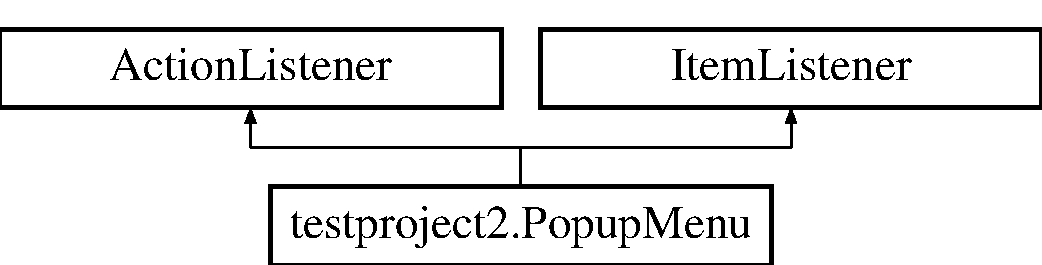
\includegraphics[height=2.000000cm]{classtestproject2_1_1PopupMenu}
\end{center}
\end{figure}
\subsection*{Classes}
\begin{DoxyCompactItemize}
\item 
class {\bfseries Popup\-Listener}
\end{DoxyCompactItemize}
\subsection*{Public Member Functions}
\begin{DoxyCompactItemize}
\item 
\hypertarget{classtestproject2_1_1PopupMenu_a4f20f2c1af3962686f6521fa2e707bcb}{void {\bfseries action\-Performed} (Action\-Event e)}\label{classtestproject2_1_1PopupMenu_a4f20f2c1af3962686f6521fa2e707bcb}

\item 
\hypertarget{classtestproject2_1_1PopupMenu_a8894ca73b034049db8ee7d3d0ddc7189}{void {\bfseries item\-State\-Changed} (Item\-Event e)}\label{classtestproject2_1_1PopupMenu_a8894ca73b034049db8ee7d3d0ddc7189}

\item 
\hypertarget{classtestproject2_1_1PopupMenu_a0f1b099fae95358a03f7314228d76277}{void {\bfseries create\-Popup\-Menu} ()}\label{classtestproject2_1_1PopupMenu_a0f1b099fae95358a03f7314228d76277}

\end{DoxyCompactItemize}


\subsection{Detailed Description}
\begin{DoxyAuthor}{Author}
loganludington 
\end{DoxyAuthor}


The documentation for this class was generated from the following file\-:\begin{DoxyCompactItemize}
\item 
branches/\-Testing\-Branch/\-Auto\-Fill\-Testing/src/testproject2/Popup\-Menu.\-java\end{DoxyCompactItemize}

\hypertarget{classcom_1_1casual__dev_1_1libpitX_1_1PrintPit}{\section{com.\-casual\-\_\-dev.\-libpit\-X.\-Print\-Pit Class Reference}
\label{classcom_1_1casual__dev_1_1libpitX_1_1PrintPit}\index{com.\-casual\-\_\-dev.\-libpit\-X.\-Print\-Pit@{com.\-casual\-\_\-dev.\-libpit\-X.\-Print\-Pit}}
}
\subsection*{Static Public Member Functions}
\begin{DoxyCompactItemize}
\item 
static void \hyperlink{classcom_1_1casual__dev_1_1libpitX_1_1PrintPit_a98038df451dc85f57d6d7c47f0c7d242}{main} (String args\mbox{[}$\,$\mbox{]})
\end{DoxyCompactItemize}


\subsection{Detailed Description}
\begin{DoxyAuthor}{Author}
adamoutler 
\end{DoxyAuthor}


\subsection{Member Function Documentation}
\hypertarget{classcom_1_1casual__dev_1_1libpitX_1_1PrintPit_a98038df451dc85f57d6d7c47f0c7d242}{\index{com\-::casual\-\_\-dev\-::libpit\-X\-::\-Print\-Pit@{com\-::casual\-\_\-dev\-::libpit\-X\-::\-Print\-Pit}!main@{main}}
\index{main@{main}!com::casual_dev::libpitX::PrintPit@{com\-::casual\-\_\-dev\-::libpit\-X\-::\-Print\-Pit}}
\subsubsection[{main}]{\setlength{\rightskip}{0pt plus 5cm}static void com.\-casual\-\_\-dev.\-libpit\-X.\-Print\-Pit.\-main (
\begin{DoxyParamCaption}
\item[{String}]{args\mbox{[}$\,$\mbox{]}}
\end{DoxyParamCaption}
)\hspace{0.3cm}{\ttfamily [static]}}}\label{classcom_1_1casual__dev_1_1libpitX_1_1PrintPit_a98038df451dc85f57d6d7c47f0c7d242}
Analyzes and prints a pit file in print-\/pit format.


\begin{DoxyParams}{Parameters}
{\em args} & filename to analyze \\
\hline
\end{DoxyParams}


The documentation for this class was generated from the following file\-:\begin{DoxyCompactItemize}
\item 
trunk/\-X/libpit\-X/src/com/casual\-\_\-dev/libpit\-X/Print\-Pit.\-java\end{DoxyCompactItemize}

\hypertarget{classCASUAL_1_1archiving_1_1libpit_1_1PrintPit}{\section{C\-A\-S\-U\-A\-L.\-archiving.\-libpit.\-Print\-Pit Class Reference}
\label{classCASUAL_1_1archiving_1_1libpit_1_1PrintPit}\index{C\-A\-S\-U\-A\-L.\-archiving.\-libpit.\-Print\-Pit@{C\-A\-S\-U\-A\-L.\-archiving.\-libpit.\-Print\-Pit}}
}
\subsection*{Static Public Member Functions}
\begin{DoxyCompactItemize}
\item 
static void \hyperlink{classCASUAL_1_1archiving_1_1libpit_1_1PrintPit_a377185e8a565e84b2f1d8f4fe57aad4f}{main} (String args\mbox{[}$\,$\mbox{]})
\end{DoxyCompactItemize}


\subsection{Detailed Description}
\begin{DoxyAuthor}{Author}
adamoutler 
\end{DoxyAuthor}


\subsection{Member Function Documentation}
\hypertarget{classCASUAL_1_1archiving_1_1libpit_1_1PrintPit_a377185e8a565e84b2f1d8f4fe57aad4f}{\index{C\-A\-S\-U\-A\-L\-::archiving\-::libpit\-::\-Print\-Pit@{C\-A\-S\-U\-A\-L\-::archiving\-::libpit\-::\-Print\-Pit}!main@{main}}
\index{main@{main}!CASUAL::archiving::libpit::PrintPit@{C\-A\-S\-U\-A\-L\-::archiving\-::libpit\-::\-Print\-Pit}}
\subsubsection[{main}]{\setlength{\rightskip}{0pt plus 5cm}static void C\-A\-S\-U\-A\-L.\-archiving.\-libpit.\-Print\-Pit.\-main (
\begin{DoxyParamCaption}
\item[{String}]{args\mbox{[}$\,$\mbox{]}}
\end{DoxyParamCaption}
)\hspace{0.3cm}{\ttfamily [static]}}}\label{classCASUAL_1_1archiving_1_1libpit_1_1PrintPit_a377185e8a565e84b2f1d8f4fe57aad4f}
Analyzes and prints a pit file in print-\/pit format.


\begin{DoxyParams}{Parameters}
{\em args} & filename to analyze \\
\hline
\end{DoxyParams}


The documentation for this class was generated from the following file\-:\begin{DoxyCompactItemize}
\item 
trunk/\-C\-A\-S\-U\-A\-Lcore/src/\-C\-A\-S\-U\-A\-L/archiving/libpit/Print\-Pit.\-java\end{DoxyCompactItemize}

\hypertarget{classCASUAL_1_1archiving_1_1libpit_1_1PrintPitTest}{\section{C\-A\-S\-U\-A\-L.\-archiving.\-libpit.\-Print\-Pit\-Test Class Reference}
\label{classCASUAL_1_1archiving_1_1libpit_1_1PrintPitTest}\index{C\-A\-S\-U\-A\-L.\-archiving.\-libpit.\-Print\-Pit\-Test@{C\-A\-S\-U\-A\-L.\-archiving.\-libpit.\-Print\-Pit\-Test}}
}
\subsection*{Public Member Functions}
\begin{DoxyCompactItemize}
\item 
\hypertarget{classCASUAL_1_1archiving_1_1libpit_1_1PrintPitTest_a005bbb9630e8f2235fb1e5305981763e}{void {\bfseries set\-Up} ()}\label{classCASUAL_1_1archiving_1_1libpit_1_1PrintPitTest_a005bbb9630e8f2235fb1e5305981763e}

\item 
\hypertarget{classCASUAL_1_1archiving_1_1libpit_1_1PrintPitTest_abca9206e3105cba2dff9e2166e20b797}{void {\bfseries tear\-Down} ()}\label{classCASUAL_1_1archiving_1_1libpit_1_1PrintPitTest_abca9206e3105cba2dff9e2166e20b797}

\item 
void \hyperlink{classCASUAL_1_1archiving_1_1libpit_1_1PrintPitTest_a8cda7943146d8bcd23cef645058a5ab0}{test\-Main} ()
\end{DoxyCompactItemize}
\subsection*{Static Public Member Functions}
\begin{DoxyCompactItemize}
\item 
\hypertarget{classCASUAL_1_1archiving_1_1libpit_1_1PrintPitTest_a5b223af9f63aa53afab25f0503aa3125}{static void {\bfseries set\-Up\-Class} ()}\label{classCASUAL_1_1archiving_1_1libpit_1_1PrintPitTest_a5b223af9f63aa53afab25f0503aa3125}

\item 
\hypertarget{classCASUAL_1_1archiving_1_1libpit_1_1PrintPitTest_a35965daf3bd2a0a1f076f0c236425a74}{static void {\bfseries tear\-Down\-Class} ()}\label{classCASUAL_1_1archiving_1_1libpit_1_1PrintPitTest_a35965daf3bd2a0a1f076f0c236425a74}

\end{DoxyCompactItemize}


\subsection{Detailed Description}
\begin{DoxyAuthor}{Author}
adamoutler 
\end{DoxyAuthor}


\subsection{Member Function Documentation}
\hypertarget{classCASUAL_1_1archiving_1_1libpit_1_1PrintPitTest_a8cda7943146d8bcd23cef645058a5ab0}{\index{C\-A\-S\-U\-A\-L\-::archiving\-::libpit\-::\-Print\-Pit\-Test@{C\-A\-S\-U\-A\-L\-::archiving\-::libpit\-::\-Print\-Pit\-Test}!test\-Main@{test\-Main}}
\index{test\-Main@{test\-Main}!CASUAL::archiving::libpit::PrintPitTest@{C\-A\-S\-U\-A\-L\-::archiving\-::libpit\-::\-Print\-Pit\-Test}}
\subsubsection[{test\-Main}]{\setlength{\rightskip}{0pt plus 5cm}void C\-A\-S\-U\-A\-L.\-archiving.\-libpit.\-Print\-Pit\-Test.\-test\-Main (
\begin{DoxyParamCaption}
{}
\end{DoxyParamCaption}
)}}\label{classCASUAL_1_1archiving_1_1libpit_1_1PrintPitTest_a8cda7943146d8bcd23cef645058a5ab0}
Test of main method, of class \hyperlink{classCASUAL_1_1archiving_1_1libpit_1_1PrintPit}{Print\-Pit}. 

The documentation for this class was generated from the following file\-:\begin{DoxyCompactItemize}
\item 
trunk/\-C\-A\-S\-U\-A\-Lcore/test/\-C\-A\-S\-U\-A\-L/archiving/libpit/Print\-Pit\-Test.\-java\end{DoxyCompactItemize}

\hypertarget{enumdevicedetector_1_1msiexecInterface_1_1RepairOptions}{\section{devicedetector.\-msiexec\-Interface.\-Repair\-Options Enum Reference}
\label{enumdevicedetector_1_1msiexecInterface_1_1RepairOptions}\index{devicedetector.\-msiexec\-Interface.\-Repair\-Options@{devicedetector.\-msiexec\-Interface.\-Repair\-Options}}
}
\subsection*{Public Attributes}
\begin{DoxyCompactItemize}
\item 
\hypertarget{enumdevicedetector_1_1msiexecInterface_1_1RepairOptions_a1ae6276c993b0e971300c0152a4811e0}{{\bfseries O\-N\-L\-Y\-\_\-\-I\-F\-\_\-\-M\-I\-S\-S\-I\-N\-G}}\label{enumdevicedetector_1_1msiexecInterface_1_1RepairOptions_a1ae6276c993b0e971300c0152a4811e0}

\item 
\hypertarget{enumdevicedetector_1_1msiexecInterface_1_1RepairOptions_ab04b34fbec3a1591235637df36c6972f}{{\bfseries O\-L\-D\-E\-R\-\_\-\-V\-E\-R\-S\-I\-O\-N}}\label{enumdevicedetector_1_1msiexecInterface_1_1RepairOptions_ab04b34fbec3a1591235637df36c6972f}

\item 
\hypertarget{enumdevicedetector_1_1msiexecInterface_1_1RepairOptions_a90d0d93089b7d50b4014d949323dd190}{{\bfseries O\-L\-D\-E\-R\-\_\-\-O\-R\-\_\-\-E\-Q\-U\-A\-L\-\_\-\-V\-E\-R\-S\-I\-O\-N}}\label{enumdevicedetector_1_1msiexecInterface_1_1RepairOptions_a90d0d93089b7d50b4014d949323dd190}

\item 
\hypertarget{enumdevicedetector_1_1msiexecInterface_1_1RepairOptions_aca9db5789f57d3fee0adc50f4ab3d9bb}{{\bfseries D\-I\-F\-F\-E\-R\-E\-N\-T\-\_\-\-V\-E\-R\-S\-I\-O\-N}}\label{enumdevicedetector_1_1msiexecInterface_1_1RepairOptions_aca9db5789f57d3fee0adc50f4ab3d9bb}

\item 
\hypertarget{enumdevicedetector_1_1msiexecInterface_1_1RepairOptions_a871cd3c5159fa108d09d035bd5d7b209}{{\bfseries C\-H\-E\-C\-K\-S\-U\-M\-\_\-\-M\-I\-S\-M\-A\-T\-C\-H}}\label{enumdevicedetector_1_1msiexecInterface_1_1RepairOptions_a871cd3c5159fa108d09d035bd5d7b209}

\item 
\hypertarget{enumdevicedetector_1_1msiexecInterface_1_1RepairOptions_ad943a0dda875bd7ad0379d05112da39d}{{\bfseries A\-L\-L\-\_\-\-F\-I\-L\-E\-S}}\label{enumdevicedetector_1_1msiexecInterface_1_1RepairOptions_ad943a0dda875bd7ad0379d05112da39d}

\end{DoxyCompactItemize}


The documentation for this enum was generated from the following file\-:\begin{DoxyCompactItemize}
\item 
branches/\-Testing\-Branch/\-Device\-Detector/src/devicedetector/msiexec\-Interface.\-java\end{DoxyCompactItemize}

\hypertarget{classReplaceLineInFile}{\section{Replace\-Line\-In\-File Class Reference}
\label{classReplaceLineInFile}\index{Replace\-Line\-In\-File@{Replace\-Line\-In\-File}}
}
\subsection*{Static Public Member Functions}
\begin{DoxyCompactItemize}
\item 
static void \hyperlink{classReplaceLineInFile_a59e429f9de8ddb7caf4d9f1047d41362}{main} (String\mbox{[}$\,$\mbox{]} args)
\end{DoxyCompactItemize}


\subsection{Detailed Description}
\begin{DoxyAuthor}{Author}
adamoutler 
\end{DoxyAuthor}


\subsection{Member Function Documentation}
\hypertarget{classReplaceLineInFile_a59e429f9de8ddb7caf4d9f1047d41362}{\index{Replace\-Line\-In\-File@{Replace\-Line\-In\-File}!main@{main}}
\index{main@{main}!ReplaceLineInFile@{Replace\-Line\-In\-File}}
\subsubsection[{main}]{\setlength{\rightskip}{0pt plus 5cm}static void Replace\-Line\-In\-File.\-main (
\begin{DoxyParamCaption}
\item[{String\mbox{[}$\,$\mbox{]}}]{args}
\end{DoxyParamCaption}
)\hspace{0.3cm}{\ttfamily [static]}}}\label{classReplaceLineInFile_a59e429f9de8ddb7caf4d9f1047d41362}
replaces entire lines in files


\begin{DoxyParams}{Parameters}
{\em args} & 1. file or folder to scan 2. old line contents to be replaced
\begin{DoxyEnumerate}
\item new line contents to be replaced 
\end{DoxyEnumerate}\\
\hline
\end{DoxyParams}


The documentation for this class was generated from the following file\-:\begin{DoxyCompactItemize}
\item 
trunk/\-C\-A\-S\-U\-A\-Lcore/\-Build\-Tasks/Replace\-Line\-In\-File.\-java\end{DoxyCompactItemize}

\hypertarget{classResolveSVNConflicts}{\section{Resolve\-S\-V\-N\-Conflicts Class Reference}
\label{classResolveSVNConflicts}\index{Resolve\-S\-V\-N\-Conflicts@{Resolve\-S\-V\-N\-Conflicts}}
}
\subsection*{Static Public Member Functions}
\begin{DoxyCompactItemize}
\item 
static void \hyperlink{classResolveSVNConflicts_a4159dc699f8721d53c294fea13435a8f}{main} (String\mbox{[}$\,$\mbox{]} args)
\end{DoxyCompactItemize}


\subsection{Detailed Description}
\begin{DoxyAuthor}{Author}
adam 
\end{DoxyAuthor}


\subsection{Member Function Documentation}
\hypertarget{classResolveSVNConflicts_a4159dc699f8721d53c294fea13435a8f}{\index{Resolve\-S\-V\-N\-Conflicts@{Resolve\-S\-V\-N\-Conflicts}!main@{main}}
\index{main@{main}!ResolveSVNConflicts@{Resolve\-S\-V\-N\-Conflicts}}
\subsubsection[{main}]{\setlength{\rightskip}{0pt plus 5cm}static void Resolve\-S\-V\-N\-Conflicts.\-main (
\begin{DoxyParamCaption}
\item[{String\mbox{[}$\,$\mbox{]}}]{args}
\end{DoxyParamCaption}
)\hspace{0.3cm}{\ttfamily [static]}}}\label{classResolveSVNConflicts_a4159dc699f8721d53c294fea13435a8f}
resolves problems in S\-V\-N


\begin{DoxyParams}{Parameters}
{\em args} & the path to the conflicting C\-A\-S\-U\-A\-L\-App files \\
\hline
\end{DoxyParams}


The documentation for this class was generated from the following file\-:\begin{DoxyCompactItemize}
\item 
trunk/\-C\-A\-S\-U\-A\-Lcore/\-Build\-Tasks/Resolve\-S\-V\-N\-Conflicts.\-java\end{DoxyCompactItemize}

\hypertarget{classCASUAL_1_1caspac_1_1Script}{\section{C\-A\-S\-U\-A\-L.\-caspac.\-Script Class Reference}
\label{classCASUAL_1_1caspac_1_1Script}\index{C\-A\-S\-U\-A\-L.\-caspac.\-Script@{C\-A\-S\-U\-A\-L.\-caspac.\-Script}}
}
\subsection*{Classes}
\begin{DoxyCompactItemize}
\item 
class \hyperlink{classCASUAL_1_1caspac_1_1Script_1_1meta}{meta}
\end{DoxyCompactItemize}
\subsection*{Public Member Functions}
\begin{DoxyCompactItemize}
\item 
\hypertarget{classCASUAL_1_1caspac_1_1Script_a817dc05b31f3530869f8ef2c5b9bc2b2}{{\bfseries Script} (\hyperlink{classCASUAL_1_1caspac_1_1Script}{Script} s)}\label{classCASUAL_1_1caspac_1_1Script_a817dc05b31f3530869f8ef2c5b9bc2b2}

\item 
\hypertarget{classCASUAL_1_1caspac_1_1Script_aa2c99871b0dad53e547497fd030a995f}{{\bfseries Script} (String name, String temp\-Dir)}\label{classCASUAL_1_1caspac_1_1Script_aa2c99871b0dad53e547497fd030a995f}

\item 
\hypertarget{classCASUAL_1_1caspac_1_1Script_ad1dadc2cf2ae9ff6f0dbcab2d7683076}{{\bfseries Script} (String name, String temp\-Dir, int type)}\label{classCASUAL_1_1caspac_1_1Script_ad1dadc2cf2ae9ff6f0dbcab2d7683076}

\item 
\hypertarget{classCASUAL_1_1caspac_1_1Script_acf090cbcc44153ce1b981630408849c7}{{\bfseries Script} (String name, String script, String discription, List$<$ File $>$ include\-Files, String temp\-Dir)}\label{classCASUAL_1_1caspac_1_1Script_acf090cbcc44153ce1b981630408849c7}

\item 
\hypertarget{classCASUAL_1_1caspac_1_1Script_ab116bbfc07a8bf5350c5a80b0cb2ec90}{{\bfseries Script} (String name, String script, String discription, List$<$ File $>$ include\-Files, Properties prop, String temp\-Dir, int type)}\label{classCASUAL_1_1caspac_1_1Script_ab116bbfc07a8bf5350c5a80b0cb2ec90}

\item 
\hypertarget{classCASUAL_1_1caspac_1_1Script_a9f76bf636c370bc47a78d42aa7b1bd6e}{{\bfseries Script} (String name, String script, String discription, List$<$ File $>$ include\-Files, Properties prop, String temp\-Dir)}\label{classCASUAL_1_1caspac_1_1Script_a9f76bf636c370bc47a78d42aa7b1bd6e}

\item 
\hypertarget{classCASUAL_1_1caspac_1_1Script_a6c9c44092063b31f1b5fa30b323e2c21}{{\bfseries Script} (String name, String script, String discription, String temp\-Dir)}\label{classCASUAL_1_1caspac_1_1Script_a6c9c44092063b31f1b5fa30b323e2c21}

\item 
\hypertarget{classCASUAL_1_1caspac_1_1Script_ae19c81a3460603a10818522d801e43ca}{\hyperlink{classCASUAL_1_1caspac_1_1Script}{Script} {\bfseries copy\-Of} (String new\-Script\-Name, String new\-Temp\-Dir)}\label{classCASUAL_1_1caspac_1_1Script_ae19c81a3460603a10818522d801e43ca}

\item 
\hypertarget{classCASUAL_1_1caspac_1_1Script_a650e8a68460d2e087028c6b7222ff61d}{boolean {\bfseries verify\-Script} ()}\label{classCASUAL_1_1caspac_1_1Script_a650e8a68460d2e087028c6b7222ff61d}

\item 
\hypertarget{classCASUAL_1_1caspac_1_1Script_a17a45608b9e9de9ab8f083781e0ef9b4}{Data\-Input\-Stream {\bfseries get\-Script\-Contents} ()}\label{classCASUAL_1_1caspac_1_1Script_a17a45608b9e9de9ab8f083781e0ef9b4}

\item 
\hypertarget{classCASUAL_1_1caspac_1_1Script_aa4417a95f79b967e72da3e7e9bd6458e}{String {\bfseries to\-String} ()}\label{classCASUAL_1_1caspac_1_1Script_aa4417a95f79b967e72da3e7e9bd6458e}

\item 
\hypertarget{classCASUAL_1_1caspac_1_1Script_a545611076ea6c3b3e8e0b2ab22e66e4f}{Runnable {\bfseries get\-Extraction\-Runnable} ()}\label{classCASUAL_1_1caspac_1_1Script_a545611076ea6c3b3e8e0b2ab22e66e4f}

\item 
\hypertarget{classCASUAL_1_1caspac_1_1Script_a335fa094032e79c5be3daa0e7cdf511c}{void {\bfseries perform\-Unzip\-After\-Script\-Zipfile\-Update} ()  throws Zip\-Exception, I\-O\-Exception }\label{classCASUAL_1_1caspac_1_1Script_a335fa094032e79c5be3daa0e7cdf511c}

\end{DoxyCompactItemize}
\subsection*{Public Attributes}
\begin{DoxyCompactItemize}
\item 
\hypertarget{classCASUAL_1_1caspac_1_1Script_ab3b3c928ac0551b948303028e66598d2}{final int {\bfseries extraction\-Method}}\label{classCASUAL_1_1caspac_1_1Script_ab3b3c928ac0551b948303028e66598d2}

\item 
\hypertarget{classCASUAL_1_1caspac_1_1Script_a48efda3482fcf8b2b3b2778495613c5e}{Object {\bfseries script\-Zip\-File}}\label{classCASUAL_1_1caspac_1_1Script_a48efda3482fcf8b2b3b2778495613c5e}

\item 
\hypertarget{classCASUAL_1_1caspac_1_1Script_a1024f90497f23ac4ef6c43426def0239}{\hyperlink{classCASUAL_1_1archiving_1_1Unzip}{Unzip} {\bfseries zipfile}}\label{classCASUAL_1_1caspac_1_1Script_a1024f90497f23ac4ef6c43426def0239}

\item 
\hypertarget{classCASUAL_1_1caspac_1_1Script_afeb97e2aa54ad52e9fe6d471083377d9}{final String {\bfseries name}}\label{classCASUAL_1_1caspac_1_1Script_afeb97e2aa54ad52e9fe6d471083377d9}

\item 
\hypertarget{classCASUAL_1_1caspac_1_1Script_abfe3164c40ad15987db21e7b0a6efb9c}{final String {\bfseries temp\-Dir}}\label{classCASUAL_1_1caspac_1_1Script_abfe3164c40ad15987db21e7b0a6efb9c}

\item 
\hypertarget{classCASUAL_1_1caspac_1_1Script_a2f578888d813eabd4d6dc4872aa3de0f}{String {\bfseries script\-Contents} = \char`\"{}\char`\"{}}\label{classCASUAL_1_1caspac_1_1Script_a2f578888d813eabd4d6dc4872aa3de0f}

\item 
\hypertarget{classCASUAL_1_1caspac_1_1Script_a8b9a3d46df38af3e319e0c2458937528}{List$<$ File $>$ {\bfseries individual\-Files} = new Array\-List$<$File$>$()}\label{classCASUAL_1_1caspac_1_1Script_a8b9a3d46df38af3e319e0c2458937528}

\item 
\hypertarget{classCASUAL_1_1caspac_1_1Script_ad432ae6788ae72a86ba665c91a611ec8}{\hyperlink{classCASUAL_1_1caspac_1_1Script_1_1meta}{meta} {\bfseries meta\-Data} = new \hyperlink{classCASUAL_1_1caspac_1_1Script_1_1meta}{meta}()}\label{classCASUAL_1_1caspac_1_1Script_ad432ae6788ae72a86ba665c91a611ec8}

\item 
\hypertarget{classCASUAL_1_1caspac_1_1Script_a2b24af13e5afbabd652d64c2a08779d5}{String {\bfseries discription} = \char`\"{}\char`\"{}}\label{classCASUAL_1_1caspac_1_1Script_a2b24af13e5afbabd652d64c2a08779d5}

\item 
\hypertarget{classCASUAL_1_1caspac_1_1Script_a344e4879129271e1b09cfec4809bcf38}{boolean {\bfseries script\-Continue} = false}\label{classCASUAL_1_1caspac_1_1Script_a344e4879129271e1b09cfec4809bcf38}

\item 
\hypertarget{classCASUAL_1_1caspac_1_1Script_ab8ee92ff986a2a9a657b97813b7ee81b}{String {\bfseries device\-Arch} = \char`\"{}\char`\"{}}\label{classCASUAL_1_1caspac_1_1Script_ab8ee92ff986a2a9a657b97813b7ee81b}

\item 
\hypertarget{classCASUAL_1_1caspac_1_1Script_a80069c0eebba9d3ee738e1b2332aeabc}{List$<$ String $>$ {\bfseries actual\-M\-D5s} = new Array\-List$<$String$>$()}\label{classCASUAL_1_1caspac_1_1Script_a80069c0eebba9d3ee738e1b2332aeabc}

\end{DoxyCompactItemize}


\subsection{Detailed Description}
\begin{DoxyAuthor}{Author}
loganludington 
\end{DoxyAuthor}


The documentation for this class was generated from the following file\-:\begin{DoxyCompactItemize}
\item 
trunk/\-C\-A\-S\-U\-A\-Lcore/src/\-C\-A\-S\-U\-A\-L/caspac/Script.\-java\end{DoxyCompactItemize}

\hypertarget{classCASCADEGUI_1_1ScriptTimeline_1_1ScriptTimelineWindow}{\section{C\-A\-S\-C\-A\-D\-E\-G\-U\-I.\-Script\-Timeline.\-Script\-Timeline\-Window Class Reference}
\label{classCASCADEGUI_1_1ScriptTimeline_1_1ScriptTimelineWindow}\index{C\-A\-S\-C\-A\-D\-E\-G\-U\-I.\-Script\-Timeline.\-Script\-Timeline\-Window@{C\-A\-S\-C\-A\-D\-E\-G\-U\-I.\-Script\-Timeline.\-Script\-Timeline\-Window}}
}
Inheritance diagram for C\-A\-S\-C\-A\-D\-E\-G\-U\-I.\-Script\-Timeline.\-Script\-Timeline\-Window\-:\begin{figure}[H]
\begin{center}
\leavevmode
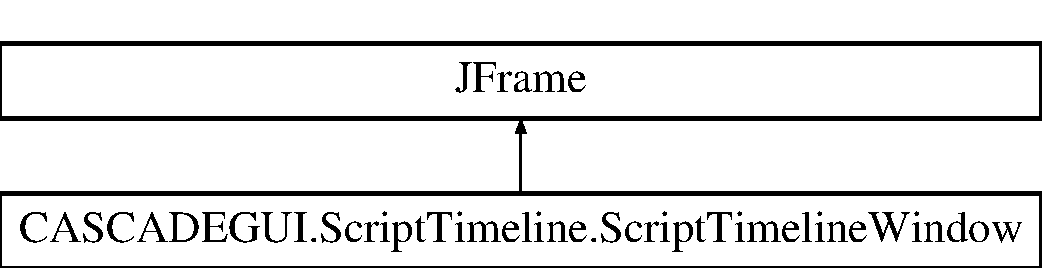
\includegraphics[height=2.000000cm]{classCASCADEGUI_1_1ScriptTimeline_1_1ScriptTimelineWindow}
\end{center}
\end{figure}
\subsection*{Classes}
\begin{DoxyCompactItemize}
\item 
class \hyperlink{classCASCADEGUI_1_1ScriptTimeline_1_1ScriptTimelineWindow_1_1Command}{Command}
\end{DoxyCompactItemize}
\subsection*{Public Member Functions}
\begin{DoxyCompactItemize}
\item 
\hyperlink{classCASCADEGUI_1_1ScriptTimeline_1_1ScriptTimelineWindow_ad93a50b0e02228b03b729891a6e1108b}{Script\-Timeline\-Window} ()
\item 
\hypertarget{classCASCADEGUI_1_1ScriptTimeline_1_1ScriptTimelineWindow_af2468ff8d75c9f1412178e969dd50455}{final void {\bfseries make\-Command\-List} ()}\label{classCASCADEGUI_1_1ScriptTimeline_1_1ScriptTimelineWindow_af2468ff8d75c9f1412178e969dd50455}

\end{DoxyCompactItemize}
\subsection*{Static Public Member Functions}
\begin{DoxyCompactItemize}
\item 
static void \hyperlink{classCASCADEGUI_1_1ScriptTimeline_1_1ScriptTimelineWindow_a63af12c553b67dc10b025320564443a5}{main} (String args\mbox{[}$\,$\mbox{]})
\end{DoxyCompactItemize}


\subsection{Detailed Description}
\begin{DoxyAuthor}{Author}
loganludington 
\end{DoxyAuthor}


\subsection{Constructor \& Destructor Documentation}
\hypertarget{classCASCADEGUI_1_1ScriptTimeline_1_1ScriptTimelineWindow_ad93a50b0e02228b03b729891a6e1108b}{\index{C\-A\-S\-C\-A\-D\-E\-G\-U\-I\-::\-Script\-Timeline\-::\-Script\-Timeline\-Window@{C\-A\-S\-C\-A\-D\-E\-G\-U\-I\-::\-Script\-Timeline\-::\-Script\-Timeline\-Window}!Script\-Timeline\-Window@{Script\-Timeline\-Window}}
\index{Script\-Timeline\-Window@{Script\-Timeline\-Window}!CASCADEGUI::ScriptTimeline::ScriptTimelineWindow@{C\-A\-S\-C\-A\-D\-E\-G\-U\-I\-::\-Script\-Timeline\-::\-Script\-Timeline\-Window}}
\subsubsection[{Script\-Timeline\-Window}]{\setlength{\rightskip}{0pt plus 5cm}C\-A\-S\-C\-A\-D\-E\-G\-U\-I.\-Script\-Timeline.\-Script\-Timeline\-Window.\-Script\-Timeline\-Window (
\begin{DoxyParamCaption}
{}
\end{DoxyParamCaption}
)}}\label{classCASCADEGUI_1_1ScriptTimeline_1_1ScriptTimelineWindow_ad93a50b0e02228b03b729891a6e1108b}
Creates new form C\-A\-S\-C\-A\-D\-E\-G\-U\-I\-Script\-Timeline 

\subsection{Member Function Documentation}
\hypertarget{classCASCADEGUI_1_1ScriptTimeline_1_1ScriptTimelineWindow_a63af12c553b67dc10b025320564443a5}{\index{C\-A\-S\-C\-A\-D\-E\-G\-U\-I\-::\-Script\-Timeline\-::\-Script\-Timeline\-Window@{C\-A\-S\-C\-A\-D\-E\-G\-U\-I\-::\-Script\-Timeline\-::\-Script\-Timeline\-Window}!main@{main}}
\index{main@{main}!CASCADEGUI::ScriptTimeline::ScriptTimelineWindow@{C\-A\-S\-C\-A\-D\-E\-G\-U\-I\-::\-Script\-Timeline\-::\-Script\-Timeline\-Window}}
\subsubsection[{main}]{\setlength{\rightskip}{0pt plus 5cm}static void C\-A\-S\-C\-A\-D\-E\-G\-U\-I.\-Script\-Timeline.\-Script\-Timeline\-Window.\-main (
\begin{DoxyParamCaption}
\item[{String}]{args\mbox{[}$\,$\mbox{]}}
\end{DoxyParamCaption}
)\hspace{0.3cm}{\ttfamily [static]}}}\label{classCASCADEGUI_1_1ScriptTimeline_1_1ScriptTimelineWindow_a63af12c553b67dc10b025320564443a5}

\begin{DoxyParams}{Parameters}
{\em args} & the command line arguments \\
\hline
\end{DoxyParams}


The documentation for this class was generated from the following file\-:\begin{DoxyCompactItemize}
\item 
trunk/\-C\-A\-S\-C\-A\-D\-E/\-C\-A\-S\-C\-A\-D\-E-\/\-G\-U\-I/src/\-C\-A\-S\-C\-A\-D\-E\-G\-U\-I/\-Script\-Timeline/Script\-Timeline\-Window.\-java\end{DoxyCompactItemize}

\hypertarget{classCASUAL_1_1crypto_1_1SHA256sum}{\section{C\-A\-S\-U\-A\-L.\-crypto.\-S\-H\-A256sum Class Reference}
\label{classCASUAL_1_1crypto_1_1SHA256sum}\index{C\-A\-S\-U\-A\-L.\-crypto.\-S\-H\-A256sum@{C\-A\-S\-U\-A\-L.\-crypto.\-S\-H\-A256sum}}
}
\subsection*{Public Member Functions}
\begin{DoxyCompactItemize}
\item 
\hyperlink{classCASUAL_1_1crypto_1_1SHA256sum_afc1d07faf79184606a8af15153c430e2}{S\-H\-A256sum} (String s)  throws I\-O\-Exception 
\item 
\hyperlink{classCASUAL_1_1crypto_1_1SHA256sum_ac400cc047e8571a90385f233a4ac15b6}{S\-H\-A256sum} (Input\-Stream is)  throws I\-O\-Exception 
\item 
\hyperlink{classCASUAL_1_1crypto_1_1SHA256sum_ad4848f903e6697b02b6232305eb0c958}{S\-H\-A256sum} (File f)  throws File\-Not\-Found\-Exception, I\-O\-Exception 
\item 
String \hyperlink{classCASUAL_1_1crypto_1_1SHA256sum_aac8a59bd709fff8830cbde5f522c4154}{get\-Linux\-Sum} (String filename)
\item 
String \hyperlink{classCASUAL_1_1crypto_1_1SHA256sum_a8deae101346f9a0a66ca8c3b0d2db1df}{get\-Sha256} ()  throws I\-O\-Exception, No\-Such\-Algorithm\-Exception 
\end{DoxyCompactItemize}
\subsection*{Static Public Member Functions}
\begin{DoxyCompactItemize}
\item 
static String \hyperlink{classCASUAL_1_1crypto_1_1SHA256sum_a54c94bb634aeea42b0bf8705afc7a8fb}{get\-Linux\-Sum} (File file)
\item 
static String \hyperlink{classCASUAL_1_1crypto_1_1SHA256sum_a0f1178a4624b6576e5f7e56b2a2df813}{get\-Name} (String sha256sum)
\item 
static String \hyperlink{classCASUAL_1_1crypto_1_1SHA256sum_ac56c9bd745fb0e31abb7a88acd2f8f35}{get\-Sum} (String sha256sum)
\item 
static String \hyperlink{classCASUAL_1_1crypto_1_1SHA256sum_a69c267e92b86486de7152159ff51d26c}{bytes\-To\-Hex} (byte\mbox{[}$\,$\mbox{]} bytes)
\item 
static String \hyperlink{classCASUAL_1_1crypto_1_1SHA256sum_a68756d611d2cb8c028dfc57e1b2d4128}{format\-Linux\-Output\-S\-H\-A256\-Sum} (String sum, String name)
\end{DoxyCompactItemize}
\subsection*{Static Protected Attributes}
\begin{DoxyCompactItemize}
\item 
final static String \hyperlink{classCASUAL_1_1crypto_1_1SHA256sum_a309e69ab9c7a8d10259e1f4683c7d693}{L\-I\-N\-U\-X\-S\-P\-A\-C\-E\-R} = \char`\"{} \char`\"{}
\end{DoxyCompactItemize}


\subsection{Detailed Description}
\begin{DoxyAuthor}{Author}
adam attempts to replicates linux's sha256sum.. there appears to be a problem with {\itshape Linux} when tested against test vectors from this page\-: \href{http://www.nsrl.nist.gov/testdata/}{\tt http\-://www.\-nsrl.\-nist.\-gov/testdata/} I will need to review all data and figure out how to implement this later
\end{DoxyAuthor}
ad5f9292c7bd44068b5465b48b38bf18c98b4d133e80307957e5f5c372a36f7d logo.\-xcf \begin{DoxyAuthor}{Author}
Adam Outler \href{mailto:adamoutler@gmail.com}{\tt adamoutler@gmail.\-com} 
\end{DoxyAuthor}


\subsection{Constructor \& Destructor Documentation}
\hypertarget{classCASUAL_1_1crypto_1_1SHA256sum_afc1d07faf79184606a8af15153c430e2}{\index{C\-A\-S\-U\-A\-L\-::crypto\-::\-S\-H\-A256sum@{C\-A\-S\-U\-A\-L\-::crypto\-::\-S\-H\-A256sum}!S\-H\-A256sum@{S\-H\-A256sum}}
\index{S\-H\-A256sum@{S\-H\-A256sum}!CASUAL::crypto::SHA256sum@{C\-A\-S\-U\-A\-L\-::crypto\-::\-S\-H\-A256sum}}
\subsubsection[{S\-H\-A256sum}]{\setlength{\rightskip}{0pt plus 5cm}C\-A\-S\-U\-A\-L.\-crypto.\-S\-H\-A256sum.\-S\-H\-A256sum (
\begin{DoxyParamCaption}
\item[{String}]{s}
\end{DoxyParamCaption}
) throws I\-O\-Exception}}\label{classCASUAL_1_1crypto_1_1SHA256sum_afc1d07faf79184606a8af15153c430e2}
constructor to make an S\-H\-A256 from a string 
\begin{DoxyParams}{Parameters}
{\em s} & string to sha256 \\
\hline
\end{DoxyParams}

\begin{DoxyExceptions}{Exceptions}
{\em I\-O\-Exception} & \\
\hline
\end{DoxyExceptions}
\hypertarget{classCASUAL_1_1crypto_1_1SHA256sum_ac400cc047e8571a90385f233a4ac15b6}{\index{C\-A\-S\-U\-A\-L\-::crypto\-::\-S\-H\-A256sum@{C\-A\-S\-U\-A\-L\-::crypto\-::\-S\-H\-A256sum}!S\-H\-A256sum@{S\-H\-A256sum}}
\index{S\-H\-A256sum@{S\-H\-A256sum}!CASUAL::crypto::SHA256sum@{C\-A\-S\-U\-A\-L\-::crypto\-::\-S\-H\-A256sum}}
\subsubsection[{S\-H\-A256sum}]{\setlength{\rightskip}{0pt plus 5cm}C\-A\-S\-U\-A\-L.\-crypto.\-S\-H\-A256sum.\-S\-H\-A256sum (
\begin{DoxyParamCaption}
\item[{Input\-Stream}]{is}
\end{DoxyParamCaption}
) throws I\-O\-Exception}}\label{classCASUAL_1_1crypto_1_1SHA256sum_ac400cc047e8571a90385f233a4ac15b6}
constructor to make an S\-H\-A256 from an Input\-Stream 
\begin{DoxyParams}{Parameters}
{\em is} & inputstream to sha256 \\
\hline
\end{DoxyParams}

\begin{DoxyExceptions}{Exceptions}
{\em I\-O\-Exception} & \\
\hline
\end{DoxyExceptions}
\hypertarget{classCASUAL_1_1crypto_1_1SHA256sum_ad4848f903e6697b02b6232305eb0c958}{\index{C\-A\-S\-U\-A\-L\-::crypto\-::\-S\-H\-A256sum@{C\-A\-S\-U\-A\-L\-::crypto\-::\-S\-H\-A256sum}!S\-H\-A256sum@{S\-H\-A256sum}}
\index{S\-H\-A256sum@{S\-H\-A256sum}!CASUAL::crypto::SHA256sum@{C\-A\-S\-U\-A\-L\-::crypto\-::\-S\-H\-A256sum}}
\subsubsection[{S\-H\-A256sum}]{\setlength{\rightskip}{0pt plus 5cm}C\-A\-S\-U\-A\-L.\-crypto.\-S\-H\-A256sum.\-S\-H\-A256sum (
\begin{DoxyParamCaption}
\item[{File}]{f}
\end{DoxyParamCaption}
) throws File\-Not\-Found\-Exception, I\-O\-Exception}}\label{classCASUAL_1_1crypto_1_1SHA256sum_ad4848f903e6697b02b6232305eb0c958}
constructor to sha256 a file 
\begin{DoxyParams}{Parameters}
{\em f} & file to digest \\
\hline
\end{DoxyParams}

\begin{DoxyExceptions}{Exceptions}
{\em File\-Not\-Found\-Exception} & \\
\hline
{\em I\-O\-Exception} & \\
\hline
\end{DoxyExceptions}


\subsection{Member Function Documentation}
\hypertarget{classCASUAL_1_1crypto_1_1SHA256sum_a69c267e92b86486de7152159ff51d26c}{\index{C\-A\-S\-U\-A\-L\-::crypto\-::\-S\-H\-A256sum@{C\-A\-S\-U\-A\-L\-::crypto\-::\-S\-H\-A256sum}!bytes\-To\-Hex@{bytes\-To\-Hex}}
\index{bytes\-To\-Hex@{bytes\-To\-Hex}!CASUAL::crypto::SHA256sum@{C\-A\-S\-U\-A\-L\-::crypto\-::\-S\-H\-A256sum}}
\subsubsection[{bytes\-To\-Hex}]{\setlength{\rightskip}{0pt plus 5cm}static String C\-A\-S\-U\-A\-L.\-crypto.\-S\-H\-A256sum.\-bytes\-To\-Hex (
\begin{DoxyParamCaption}
\item[{byte\mbox{[}$\,$\mbox{]}}]{bytes}
\end{DoxyParamCaption}
)\hspace{0.3cm}{\ttfamily [static]}}}\label{classCASUAL_1_1crypto_1_1SHA256sum_a69c267e92b86486de7152159ff51d26c}
converts a byte array to hexadecimal output 
\begin{DoxyParams}{Parameters}
{\em bytes} & to be turned into hex \\
\hline
\end{DoxyParams}
\begin{DoxyReturn}{Returns}
hex string from bytes 
\end{DoxyReturn}
\hypertarget{classCASUAL_1_1crypto_1_1SHA256sum_a68756d611d2cb8c028dfc57e1b2d4128}{\index{C\-A\-S\-U\-A\-L\-::crypto\-::\-S\-H\-A256sum@{C\-A\-S\-U\-A\-L\-::crypto\-::\-S\-H\-A256sum}!format\-Linux\-Output\-S\-H\-A256\-Sum@{format\-Linux\-Output\-S\-H\-A256\-Sum}}
\index{format\-Linux\-Output\-S\-H\-A256\-Sum@{format\-Linux\-Output\-S\-H\-A256\-Sum}!CASUAL::crypto::SHA256sum@{C\-A\-S\-U\-A\-L\-::crypto\-::\-S\-H\-A256sum}}
\subsubsection[{format\-Linux\-Output\-S\-H\-A256\-Sum}]{\setlength{\rightskip}{0pt plus 5cm}static String C\-A\-S\-U\-A\-L.\-crypto.\-S\-H\-A256sum.\-format\-Linux\-Output\-S\-H\-A256\-Sum (
\begin{DoxyParamCaption}
\item[{String}]{sum, }
\item[{String}]{name}
\end{DoxyParamCaption}
)\hspace{0.3cm}{\ttfamily [static]}}}\label{classCASUAL_1_1crypto_1_1SHA256sum_a68756d611d2cb8c028dfc57e1b2d4128}
formats a sha256sum from a sum and a filename 
\begin{DoxyParams}{Parameters}
{\em sum} & the sha256 sum \\
\hline
{\em name} & the file name \\
\hline
\end{DoxyParams}
\begin{DoxyReturn}{Returns}
equal to command line output from linux sha256sum command 
\end{DoxyReturn}
\hypertarget{classCASUAL_1_1crypto_1_1SHA256sum_aac8a59bd709fff8830cbde5f522c4154}{\index{C\-A\-S\-U\-A\-L\-::crypto\-::\-S\-H\-A256sum@{C\-A\-S\-U\-A\-L\-::crypto\-::\-S\-H\-A256sum}!get\-Linux\-Sum@{get\-Linux\-Sum}}
\index{get\-Linux\-Sum@{get\-Linux\-Sum}!CASUAL::crypto::SHA256sum@{C\-A\-S\-U\-A\-L\-::crypto\-::\-S\-H\-A256sum}}
\subsubsection[{get\-Linux\-Sum}]{\setlength{\rightskip}{0pt plus 5cm}String C\-A\-S\-U\-A\-L.\-crypto.\-S\-H\-A256sum.\-get\-Linux\-Sum (
\begin{DoxyParamCaption}
\item[{String}]{filename}
\end{DoxyParamCaption}
)}}\label{classCASUAL_1_1crypto_1_1SHA256sum_aac8a59bd709fff8830cbde5f522c4154}
returns S\-H\-A256 sum in standard linux command line format 
\begin{DoxyParams}{Parameters}
{\em filename} & to use for filename \\
\hline
\end{DoxyParams}
\begin{DoxyReturn}{Returns}
linux sha256sum output 
\end{DoxyReturn}
\hypertarget{classCASUAL_1_1crypto_1_1SHA256sum_a54c94bb634aeea42b0bf8705afc7a8fb}{\index{C\-A\-S\-U\-A\-L\-::crypto\-::\-S\-H\-A256sum@{C\-A\-S\-U\-A\-L\-::crypto\-::\-S\-H\-A256sum}!get\-Linux\-Sum@{get\-Linux\-Sum}}
\index{get\-Linux\-Sum@{get\-Linux\-Sum}!CASUAL::crypto::SHA256sum@{C\-A\-S\-U\-A\-L\-::crypto\-::\-S\-H\-A256sum}}
\subsubsection[{get\-Linux\-Sum}]{\setlength{\rightskip}{0pt plus 5cm}static String C\-A\-S\-U\-A\-L.\-crypto.\-S\-H\-A256sum.\-get\-Linux\-Sum (
\begin{DoxyParamCaption}
\item[{File}]{file}
\end{DoxyParamCaption}
)\hspace{0.3cm}{\ttfamily [static]}}}\label{classCASUAL_1_1crypto_1_1SHA256sum_a54c94bb634aeea42b0bf8705afc7a8fb}
returns S\-H\-A256 sum in standard linux command line format 
\begin{DoxyParams}{Parameters}
{\em file} & to use for filename \\
\hline
\end{DoxyParams}
\begin{DoxyReturn}{Returns}
linux sha256sum output 
\end{DoxyReturn}
\hypertarget{classCASUAL_1_1crypto_1_1SHA256sum_a0f1178a4624b6576e5f7e56b2a2df813}{\index{C\-A\-S\-U\-A\-L\-::crypto\-::\-S\-H\-A256sum@{C\-A\-S\-U\-A\-L\-::crypto\-::\-S\-H\-A256sum}!get\-Name@{get\-Name}}
\index{get\-Name@{get\-Name}!CASUAL::crypto::SHA256sum@{C\-A\-S\-U\-A\-L\-::crypto\-::\-S\-H\-A256sum}}
\subsubsection[{get\-Name}]{\setlength{\rightskip}{0pt plus 5cm}static String C\-A\-S\-U\-A\-L.\-crypto.\-S\-H\-A256sum.\-get\-Name (
\begin{DoxyParamCaption}
\item[{String}]{sha256sum}
\end{DoxyParamCaption}
)\hspace{0.3cm}{\ttfamily [static]}}}\label{classCASUAL_1_1crypto_1_1SHA256sum_a0f1178a4624b6576e5f7e56b2a2df813}
gets the filename from a commandline sha256sum output 
\begin{DoxyParams}{Parameters}
{\em sha256sum} & linux sha256sum to extract name from \\
\hline
\end{DoxyParams}
\begin{DoxyReturn}{Returns}
name of file mentioned in sha256sum 
\end{DoxyReturn}
\hypertarget{classCASUAL_1_1crypto_1_1SHA256sum_a8deae101346f9a0a66ca8c3b0d2db1df}{\index{C\-A\-S\-U\-A\-L\-::crypto\-::\-S\-H\-A256sum@{C\-A\-S\-U\-A\-L\-::crypto\-::\-S\-H\-A256sum}!get\-Sha256@{get\-Sha256}}
\index{get\-Sha256@{get\-Sha256}!CASUAL::crypto::SHA256sum@{C\-A\-S\-U\-A\-L\-::crypto\-::\-S\-H\-A256sum}}
\subsubsection[{get\-Sha256}]{\setlength{\rightskip}{0pt plus 5cm}String C\-A\-S\-U\-A\-L.\-crypto.\-S\-H\-A256sum.\-get\-Sha256 (
\begin{DoxyParamCaption}
{}
\end{DoxyParamCaption}
) throws I\-O\-Exception, No\-Such\-Algorithm\-Exception}}\label{classCASUAL_1_1crypto_1_1SHA256sum_a8deae101346f9a0a66ca8c3b0d2db1df}
does the S\-H\-A256

\begin{DoxyReturn}{Returns}
hex string representation of the input 
\end{DoxyReturn}

\begin{DoxyExceptions}{Exceptions}
{\em I\-O\-Exception} & \\
\hline
{\em No\-Such\-Algorithm\-Exception} & \\
\hline
\end{DoxyExceptions}
\hypertarget{classCASUAL_1_1crypto_1_1SHA256sum_ac56c9bd745fb0e31abb7a88acd2f8f35}{\index{C\-A\-S\-U\-A\-L\-::crypto\-::\-S\-H\-A256sum@{C\-A\-S\-U\-A\-L\-::crypto\-::\-S\-H\-A256sum}!get\-Sum@{get\-Sum}}
\index{get\-Sum@{get\-Sum}!CASUAL::crypto::SHA256sum@{C\-A\-S\-U\-A\-L\-::crypto\-::\-S\-H\-A256sum}}
\subsubsection[{get\-Sum}]{\setlength{\rightskip}{0pt plus 5cm}static String C\-A\-S\-U\-A\-L.\-crypto.\-S\-H\-A256sum.\-get\-Sum (
\begin{DoxyParamCaption}
\item[{String}]{sha256sum}
\end{DoxyParamCaption}
)\hspace{0.3cm}{\ttfamily [static]}}}\label{classCASUAL_1_1crypto_1_1SHA256sum_ac56c9bd745fb0e31abb7a88acd2f8f35}
gets the sha256sum portion of a commandline sha256 output 
\begin{DoxyParams}{Parameters}
{\em sha256sum} & linux sha256sum to extract sum from \\
\hline
\end{DoxyParams}
\begin{DoxyReturn}{Returns}
sum portion of command line sha256 output 
\end{DoxyReturn}


\subsection{Member Data Documentation}
\hypertarget{classCASUAL_1_1crypto_1_1SHA256sum_a309e69ab9c7a8d10259e1f4683c7d693}{\index{C\-A\-S\-U\-A\-L\-::crypto\-::\-S\-H\-A256sum@{C\-A\-S\-U\-A\-L\-::crypto\-::\-S\-H\-A256sum}!L\-I\-N\-U\-X\-S\-P\-A\-C\-E\-R@{L\-I\-N\-U\-X\-S\-P\-A\-C\-E\-R}}
\index{L\-I\-N\-U\-X\-S\-P\-A\-C\-E\-R@{L\-I\-N\-U\-X\-S\-P\-A\-C\-E\-R}!CASUAL::crypto::SHA256sum@{C\-A\-S\-U\-A\-L\-::crypto\-::\-S\-H\-A256sum}}
\subsubsection[{L\-I\-N\-U\-X\-S\-P\-A\-C\-E\-R}]{\setlength{\rightskip}{0pt plus 5cm}final static String C\-A\-S\-U\-A\-L.\-crypto.\-S\-H\-A256sum.\-L\-I\-N\-U\-X\-S\-P\-A\-C\-E\-R = \char`\"{} \char`\"{}\hspace{0.3cm}{\ttfamily [static]}, {\ttfamily [protected]}}}\label{classCASUAL_1_1crypto_1_1SHA256sum_a309e69ab9c7a8d10259e1f4683c7d693}
spacer used to separate S\-H\-A256 and filename in standard sha256sum 

The documentation for this class was generated from the following file\-:\begin{DoxyCompactItemize}
\item 
trunk/\-C\-A\-S\-U\-A\-Lcore/src/\-C\-A\-S\-U\-A\-L/crypto/S\-H\-A256sum.\-java\end{DoxyCompactItemize}

\hypertarget{classCASUAL_1_1crypto_1_1SHA256sumTest}{\section{C\-A\-S\-U\-A\-L.\-crypto.\-S\-H\-A256sum\-Test Class Reference}
\label{classCASUAL_1_1crypto_1_1SHA256sumTest}\index{C\-A\-S\-U\-A\-L.\-crypto.\-S\-H\-A256sum\-Test@{C\-A\-S\-U\-A\-L.\-crypto.\-S\-H\-A256sum\-Test}}
}
\subsection*{Public Member Functions}
\begin{DoxyCompactItemize}
\item 
\hypertarget{classCASUAL_1_1crypto_1_1SHA256sumTest_a47ee188a29eff12683da6c241a2cc5d0}{void {\bfseries set\-Up} ()}\label{classCASUAL_1_1crypto_1_1SHA256sumTest_a47ee188a29eff12683da6c241a2cc5d0}

\item 
\hypertarget{classCASUAL_1_1crypto_1_1SHA256sumTest_a133bfddcf23c02f7682b54c159766c7d}{void {\bfseries tear\-Down} ()}\label{classCASUAL_1_1crypto_1_1SHA256sumTest_a133bfddcf23c02f7682b54c159766c7d}

\item 
void \hyperlink{classCASUAL_1_1crypto_1_1SHA256sumTest_aa32bc5a04f72608f889b6fa3d9137864}{test\-Get\-Name} ()
\item 
\hypertarget{classCASUAL_1_1crypto_1_1SHA256sumTest_a6d7d1acf6c4e51509ae4ae44a7f413e2}{void {\bfseries test\-String} ()}\label{classCASUAL_1_1crypto_1_1SHA256sumTest_a6d7d1acf6c4e51509ae4ae44a7f413e2}

\item 
void \hyperlink{classCASUAL_1_1crypto_1_1SHA256sumTest_aa64bfb4fd5c838fb57fa854ae88e616c}{test\-Get\-Sum} ()
\item 
void \hyperlink{classCASUAL_1_1crypto_1_1SHA256sumTest_a312c80659b205ac950704ea54c51d648}{test\-Bytes\-To\-Hex} ()
\item 
\hypertarget{classCASUAL_1_1crypto_1_1SHA256sumTest_ad48c86e6a4af45643ffe4059b2e69127}{void {\bfseries get\-Linux\-Test\-Sum} ()}\label{classCASUAL_1_1crypto_1_1SHA256sumTest_ad48c86e6a4af45643ffe4059b2e69127}

\item 
\hypertarget{classCASUAL_1_1crypto_1_1SHA256sumTest_a892d1f9d57ea82598025227cfa9f9364}{void {\bfseries false\-Equals\-True} ()}\label{classCASUAL_1_1crypto_1_1SHA256sumTest_a892d1f9d57ea82598025227cfa9f9364}

\item 
\hypertarget{classCASUAL_1_1crypto_1_1SHA256sumTest_a5251d3dc892ae7ccf10bdc31cfe988bc}{void {\bfseries get\-Linux\-Test\-Sum\-From\-String} ()}\label{classCASUAL_1_1crypto_1_1SHA256sumTest_a5251d3dc892ae7ccf10bdc31cfe988bc}

\item 
\hypertarget{classCASUAL_1_1crypto_1_1SHA256sumTest_a5a7da46a949a3cd9b21d93ae2f4401a4}{void {\bfseries get\-Linux\-Test\-Sum\-From\-File} ()}\label{classCASUAL_1_1crypto_1_1SHA256sumTest_a5a7da46a949a3cd9b21d93ae2f4401a4}

\end{DoxyCompactItemize}
\subsection*{Static Public Member Functions}
\begin{DoxyCompactItemize}
\item 
\hypertarget{classCASUAL_1_1crypto_1_1SHA256sumTest_a06a1d0f62fa9ada30ee9a8cd4bcfb4cc}{static void {\bfseries set\-Up\-Class} ()}\label{classCASUAL_1_1crypto_1_1SHA256sumTest_a06a1d0f62fa9ada30ee9a8cd4bcfb4cc}

\item 
\hypertarget{classCASUAL_1_1crypto_1_1SHA256sumTest_a8a5c2572e4645b39464d7536437ce51f}{static void {\bfseries tear\-Down\-Class} ()}\label{classCASUAL_1_1crypto_1_1SHA256sumTest_a8a5c2572e4645b39464d7536437ce51f}

\end{DoxyCompactItemize}


\subsection{Detailed Description}
\begin{DoxyAuthor}{Author}
adam 
\end{DoxyAuthor}


\subsection{Member Function Documentation}
\hypertarget{classCASUAL_1_1crypto_1_1SHA256sumTest_a312c80659b205ac950704ea54c51d648}{\index{C\-A\-S\-U\-A\-L\-::crypto\-::\-S\-H\-A256sum\-Test@{C\-A\-S\-U\-A\-L\-::crypto\-::\-S\-H\-A256sum\-Test}!test\-Bytes\-To\-Hex@{test\-Bytes\-To\-Hex}}
\index{test\-Bytes\-To\-Hex@{test\-Bytes\-To\-Hex}!CASUAL::crypto::SHA256sumTest@{C\-A\-S\-U\-A\-L\-::crypto\-::\-S\-H\-A256sum\-Test}}
\subsubsection[{test\-Bytes\-To\-Hex}]{\setlength{\rightskip}{0pt plus 5cm}void C\-A\-S\-U\-A\-L.\-crypto.\-S\-H\-A256sum\-Test.\-test\-Bytes\-To\-Hex (
\begin{DoxyParamCaption}
{}
\end{DoxyParamCaption}
)}}\label{classCASUAL_1_1crypto_1_1SHA256sumTest_a312c80659b205ac950704ea54c51d648}
Test of bytes\-To\-Hex method, of class \hyperlink{classCASUAL_1_1crypto_1_1SHA256sum}{S\-H\-A256sum}. \hypertarget{classCASUAL_1_1crypto_1_1SHA256sumTest_aa32bc5a04f72608f889b6fa3d9137864}{\index{C\-A\-S\-U\-A\-L\-::crypto\-::\-S\-H\-A256sum\-Test@{C\-A\-S\-U\-A\-L\-::crypto\-::\-S\-H\-A256sum\-Test}!test\-Get\-Name@{test\-Get\-Name}}
\index{test\-Get\-Name@{test\-Get\-Name}!CASUAL::crypto::SHA256sumTest@{C\-A\-S\-U\-A\-L\-::crypto\-::\-S\-H\-A256sum\-Test}}
\subsubsection[{test\-Get\-Name}]{\setlength{\rightskip}{0pt plus 5cm}void C\-A\-S\-U\-A\-L.\-crypto.\-S\-H\-A256sum\-Test.\-test\-Get\-Name (
\begin{DoxyParamCaption}
{}
\end{DoxyParamCaption}
)}}\label{classCASUAL_1_1crypto_1_1SHA256sumTest_aa32bc5a04f72608f889b6fa3d9137864}
Test of get\-Name method, of class \hyperlink{classCASUAL_1_1crypto_1_1SHA256sum}{S\-H\-A256sum}. \hypertarget{classCASUAL_1_1crypto_1_1SHA256sumTest_aa64bfb4fd5c838fb57fa854ae88e616c}{\index{C\-A\-S\-U\-A\-L\-::crypto\-::\-S\-H\-A256sum\-Test@{C\-A\-S\-U\-A\-L\-::crypto\-::\-S\-H\-A256sum\-Test}!test\-Get\-Sum@{test\-Get\-Sum}}
\index{test\-Get\-Sum@{test\-Get\-Sum}!CASUAL::crypto::SHA256sumTest@{C\-A\-S\-U\-A\-L\-::crypto\-::\-S\-H\-A256sum\-Test}}
\subsubsection[{test\-Get\-Sum}]{\setlength{\rightskip}{0pt plus 5cm}void C\-A\-S\-U\-A\-L.\-crypto.\-S\-H\-A256sum\-Test.\-test\-Get\-Sum (
\begin{DoxyParamCaption}
{}
\end{DoxyParamCaption}
)}}\label{classCASUAL_1_1crypto_1_1SHA256sumTest_aa64bfb4fd5c838fb57fa854ae88e616c}
Test of get\-Sum method, of class \hyperlink{classCASUAL_1_1crypto_1_1SHA256sum}{S\-H\-A256sum}. 

The documentation for this class was generated from the following file\-:\begin{DoxyCompactItemize}
\item 
trunk/\-C\-A\-S\-U\-A\-Lcore/test/\-C\-A\-S\-U\-A\-L/crypto/S\-H\-A256sum\-Test.\-java\end{DoxyCompactItemize}

\hypertarget{classCASUAL_1_1Shell}{\section{C\-A\-S\-U\-A\-L.\-Shell Class Reference}
\label{classCASUAL_1_1Shell}\index{C\-A\-S\-U\-A\-L.\-Shell@{C\-A\-S\-U\-A\-L.\-Shell}}
}
Inheritance diagram for C\-A\-S\-U\-A\-L.\-Shell\-:\begin{figure}[H]
\begin{center}
\leavevmode
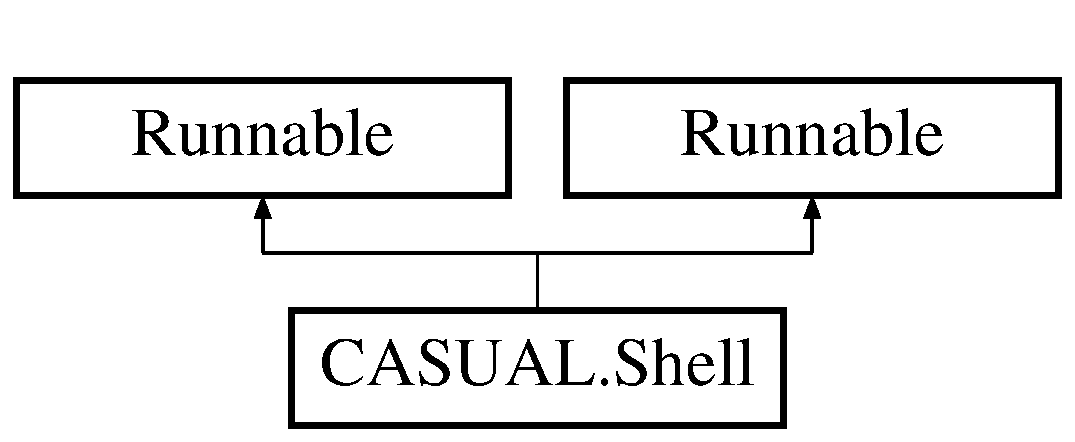
\includegraphics[height=2.000000cm]{classCASUAL_1_1Shell}
\end{center}
\end{figure}
\subsection*{Public Member Functions}
\begin{DoxyCompactItemize}
\item 
\hypertarget{classCASUAL_1_1Shell_a228ae0a36fd9bf8773b20d9ce67d186a}{String {\bfseries elevate\-Simple\-Command} (String\mbox{[}$\,$\mbox{]} cmd)}\label{classCASUAL_1_1Shell_a228ae0a36fd9bf8773b20d9ce67d186a}

\item 
\hypertarget{classCASUAL_1_1Shell_a7b3433f703f854ebccf0d0fb03ace169}{String {\bfseries send\-Shell\-Command} (String\mbox{[}$\,$\mbox{]} cmd)}\label{classCASUAL_1_1Shell_a7b3433f703f854ebccf0d0fb03ace169}

\item 
\hypertarget{classCASUAL_1_1Shell_a7b5fe192fb2f8643e0abf9be080108c6}{String {\bfseries silent\-Shell\-Command} (String\mbox{[}$\,$\mbox{]} cmd)}\label{classCASUAL_1_1Shell_a7b5fe192fb2f8643e0abf9be080108c6}

\item 
\hypertarget{classCASUAL_1_1Shell_a70d25c128178ed80debee0b6053dac4d}{String {\bfseries array\-To\-String} (String\mbox{[}$\,$\mbox{]} stringarray)}\label{classCASUAL_1_1Shell_a70d25c128178ed80debee0b6053dac4d}

\item 
\hypertarget{classCASUAL_1_1Shell_a37881bb2c0d03b14748bf0f0047053a1}{void {\bfseries live\-Shell\-Command} (String\mbox{[}$\,$\mbox{]} params)}\label{classCASUAL_1_1Shell_a37881bb2c0d03b14748bf0f0047053a1}

\item 
\hypertarget{classCASUAL_1_1Shell_ad5bcb0ff18bd7023fa763901f4410e24}{void {\bfseries live\-Background\-Shell\-Command} ()}\label{classCASUAL_1_1Shell_ad5bcb0ff18bd7023fa763901f4410e24}

\item 
\hypertarget{classCASUAL_1_1Shell_aa42ddb7317b31e55804c22fb973bbb3e}{void {\bfseries run} ()}\label{classCASUAL_1_1Shell_aa42ddb7317b31e55804c22fb973bbb3e}

\item 
\hypertarget{classCASUAL_1_1Shell_a228ae0a36fd9bf8773b20d9ce67d186a}{String {\bfseries elevate\-Simple\-Command} (String\mbox{[}$\,$\mbox{]} cmd)}\label{classCASUAL_1_1Shell_a228ae0a36fd9bf8773b20d9ce67d186a}

\item 
\hypertarget{classCASUAL_1_1Shell_a7b3433f703f854ebccf0d0fb03ace169}{String {\bfseries send\-Shell\-Command} (String\mbox{[}$\,$\mbox{]} cmd)}\label{classCASUAL_1_1Shell_a7b3433f703f854ebccf0d0fb03ace169}

\item 
\hypertarget{classCASUAL_1_1Shell_a7b5fe192fb2f8643e0abf9be080108c6}{String {\bfseries silent\-Shell\-Command} (String\mbox{[}$\,$\mbox{]} cmd)}\label{classCASUAL_1_1Shell_a7b5fe192fb2f8643e0abf9be080108c6}

\item 
\hypertarget{classCASUAL_1_1Shell_a70d25c128178ed80debee0b6053dac4d}{String {\bfseries array\-To\-String} (String\mbox{[}$\,$\mbox{]} stringarray)}\label{classCASUAL_1_1Shell_a70d25c128178ed80debee0b6053dac4d}

\item 
\hypertarget{classCASUAL_1_1Shell_a37881bb2c0d03b14748bf0f0047053a1}{void {\bfseries live\-Shell\-Command} (String\mbox{[}$\,$\mbox{]} params)}\label{classCASUAL_1_1Shell_a37881bb2c0d03b14748bf0f0047053a1}

\item 
\hypertarget{classCASUAL_1_1Shell_ad5bcb0ff18bd7023fa763901f4410e24}{void {\bfseries live\-Background\-Shell\-Command} ()}\label{classCASUAL_1_1Shell_ad5bcb0ff18bd7023fa763901f4410e24}

\item 
\hypertarget{classCASUAL_1_1Shell_aa42ddb7317b31e55804c22fb973bbb3e}{void {\bfseries run} ()}\label{classCASUAL_1_1Shell_aa42ddb7317b31e55804c22fb973bbb3e}

\item 
\hyperlink{classCASUAL_1_1Shell_a708fd05c53f187f1e8278972a2a55b5c}{Shell} ()
\item 
String \hyperlink{classCASUAL_1_1Shell_ae42f2d9c2e19a6185deff5b9600844fb}{elevate\-Simple\-Command\-With\-Message} (String\mbox{[}$\,$\mbox{]} cmd, String message)
\item 
String \hyperlink{classCASUAL_1_1Shell_a228ae0a36fd9bf8773b20d9ce67d186a}{elevate\-Simple\-Command} (String\mbox{[}$\,$\mbox{]} cmd)
\item 
String \hyperlink{classCASUAL_1_1Shell_a7b3433f703f854ebccf0d0fb03ace169}{send\-Shell\-Command} (String\mbox{[}$\,$\mbox{]} cmd)
\item 
String \hyperlink{classCASUAL_1_1Shell_abf0198707d3bbaac312a099b70896c8f}{send\-Shell\-Command\-Ignore\-Error} (String\mbox{[}$\,$\mbox{]} cmd)
\item 
String \hyperlink{classCASUAL_1_1Shell_a7b5fe192fb2f8643e0abf9be080108c6}{silent\-Shell\-Command} (String\mbox{[}$\,$\mbox{]} cmd)
\item 
String \hyperlink{classCASUAL_1_1Shell_a8bb7dfcf5e0b9fac3168bc2a89115964}{live\-Shell\-Command} (String\mbox{[}$\,$\mbox{]} params, boolean display)
\item 
void \hyperlink{classCASUAL_1_1Shell_ad5bcb0ff18bd7023fa763901f4410e24}{live\-Background\-Shell\-Command} ()
\item 
void \hyperlink{classCASUAL_1_1Shell_a23d9169e1e0e9374d1f6e34979d10378}{silent\-Background\-Shell\-Command} ()
\item 
String \hyperlink{classCASUAL_1_1Shell_a84ab38f944a2af24e3283103e80b743c}{timeout\-Shell\-Command} (final String\mbox{[}$\,$\mbox{]} cmd, int timeout)
\item 
String \hyperlink{classCASUAL_1_1Shell_a50d89a1c8176f36f111e9b259e8fb3d7}{silent\-Timeout\-Shell\-Command} (final String\mbox{[}$\,$\mbox{]} cmd, int timeout)
\item 
String \hyperlink{classCASUAL_1_1Shell_adbc863b6cf3a4606764bdc57bb86e1ed}{timeout\-Value\-Checking\-Shell\-Command} (final String\mbox{[}$\,$\mbox{]} cmd, final String\mbox{[}$\,$\mbox{]} start\-Timer\-On\-This\-In\-Line, final int timeout)
\end{DoxyCompactItemize}


\subsection{Detailed Description}
\begin{DoxyAuthor}{Author}
adam 
\end{DoxyAuthor}


\subsection{Constructor \& Destructor Documentation}
\hypertarget{classCASUAL_1_1Shell_a708fd05c53f187f1e8278972a2a55b5c}{\index{C\-A\-S\-U\-A\-L\-::\-Shell@{C\-A\-S\-U\-A\-L\-::\-Shell}!Shell@{Shell}}
\index{Shell@{Shell}!CASUAL::Shell@{C\-A\-S\-U\-A\-L\-::\-Shell}}
\subsubsection[{Shell}]{\setlength{\rightskip}{0pt plus 5cm}C\-A\-S\-U\-A\-L.\-Shell.\-Shell (
\begin{DoxyParamCaption}
{}
\end{DoxyParamCaption}
)}}\label{classCASUAL_1_1Shell_a708fd05c53f187f1e8278972a2a55b5c}
\hyperlink{classCASUAL_1_1Shell}{Shell} provides a set of methods to access \hyperlink{classCASUAL_1_1Shell}{Shell} commands in predefined ways. 

\subsection{Member Function Documentation}
\hypertarget{classCASUAL_1_1Shell_a228ae0a36fd9bf8773b20d9ce67d186a}{\index{C\-A\-S\-U\-A\-L\-::\-Shell@{C\-A\-S\-U\-A\-L\-::\-Shell}!elevate\-Simple\-Command@{elevate\-Simple\-Command}}
\index{elevate\-Simple\-Command@{elevate\-Simple\-Command}!CASUAL::Shell@{C\-A\-S\-U\-A\-L\-::\-Shell}}
\subsubsection[{elevate\-Simple\-Command}]{\setlength{\rightskip}{0pt plus 5cm}String C\-A\-S\-U\-A\-L.\-Shell.\-elevate\-Simple\-Command (
\begin{DoxyParamCaption}
\item[{String\mbox{[}$\,$\mbox{]}}]{cmd}
\end{DoxyParamCaption}
)}}\label{classCASUAL_1_1Shell_a228ae0a36fd9bf8773b20d9ce67d186a}
Attempts to elevate a shell command for any platform.


\begin{DoxyParams}{Parameters}
{\em cmd} & Array representing command and parameters to execute \\
\hline
\end{DoxyParams}
\begin{DoxyReturn}{Returns}
return from command executed 
\end{DoxyReturn}
\hypertarget{classCASUAL_1_1Shell_ae42f2d9c2e19a6185deff5b9600844fb}{\index{C\-A\-S\-U\-A\-L\-::\-Shell@{C\-A\-S\-U\-A\-L\-::\-Shell}!elevate\-Simple\-Command\-With\-Message@{elevate\-Simple\-Command\-With\-Message}}
\index{elevate\-Simple\-Command\-With\-Message@{elevate\-Simple\-Command\-With\-Message}!CASUAL::Shell@{C\-A\-S\-U\-A\-L\-::\-Shell}}
\subsubsection[{elevate\-Simple\-Command\-With\-Message}]{\setlength{\rightskip}{0pt plus 5cm}String C\-A\-S\-U\-A\-L.\-Shell.\-elevate\-Simple\-Command\-With\-Message (
\begin{DoxyParamCaption}
\item[{String\mbox{[}$\,$\mbox{]}}]{cmd, }
\item[{String}]{message}
\end{DoxyParamCaption}
)}}\label{classCASUAL_1_1Shell_ae42f2d9c2e19a6185deff5b9600844fb}
Attempts to elevate a shell command for any platform.


\begin{DoxyParams}{Parameters}
{\em cmd} & Array representing command and parameters to execute \\
\hline
{\em message} & message to be displayed to user when asked for permissions \\
\hline
\end{DoxyParams}
\begin{DoxyReturn}{Returns}
return from command executed 
\end{DoxyReturn}
\hypertarget{classCASUAL_1_1Shell_ad5bcb0ff18bd7023fa763901f4410e24}{\index{C\-A\-S\-U\-A\-L\-::\-Shell@{C\-A\-S\-U\-A\-L\-::\-Shell}!live\-Background\-Shell\-Command@{live\-Background\-Shell\-Command}}
\index{live\-Background\-Shell\-Command@{live\-Background\-Shell\-Command}!CASUAL::Shell@{C\-A\-S\-U\-A\-L\-::\-Shell}}
\subsubsection[{live\-Background\-Shell\-Command}]{\setlength{\rightskip}{0pt plus 5cm}void C\-A\-S\-U\-A\-L.\-Shell.\-live\-Background\-Shell\-Command (
\begin{DoxyParamCaption}
{}
\end{DoxyParamCaption}
)}}\label{classCASUAL_1_1Shell_ad5bcb0ff18bd7023fa763901f4410e24}
executes a command on a new thread and displays output to logging device. Takes command parameters from Statics.\-Live\-Send\-Command. \hypertarget{classCASUAL_1_1Shell_a8bb7dfcf5e0b9fac3168bc2a89115964}{\index{C\-A\-S\-U\-A\-L\-::\-Shell@{C\-A\-S\-U\-A\-L\-::\-Shell}!live\-Shell\-Command@{live\-Shell\-Command}}
\index{live\-Shell\-Command@{live\-Shell\-Command}!CASUAL::Shell@{C\-A\-S\-U\-A\-L\-::\-Shell}}
\subsubsection[{live\-Shell\-Command}]{\setlength{\rightskip}{0pt plus 5cm}String C\-A\-S\-U\-A\-L.\-Shell.\-live\-Shell\-Command (
\begin{DoxyParamCaption}
\item[{String\mbox{[}$\,$\mbox{]}}]{params, }
\item[{boolean}]{display}
\end{DoxyParamCaption}
)}}\label{classCASUAL_1_1Shell_a8bb7dfcf5e0b9fac3168bc2a89115964}
Live shell command executes a command and outputs information in real-\/time to console


\begin{DoxyParams}{Parameters}
{\em params} & command and arguments to execute \\
\hline
{\em display} & true if output should be logged to log device \\
\hline
\end{DoxyParams}
\begin{DoxyReturn}{Returns}
output from command 
\end{DoxyReturn}
\hypertarget{classCASUAL_1_1Shell_a7b3433f703f854ebccf0d0fb03ace169}{\index{C\-A\-S\-U\-A\-L\-::\-Shell@{C\-A\-S\-U\-A\-L\-::\-Shell}!send\-Shell\-Command@{send\-Shell\-Command}}
\index{send\-Shell\-Command@{send\-Shell\-Command}!CASUAL::Shell@{C\-A\-S\-U\-A\-L\-::\-Shell}}
\subsubsection[{send\-Shell\-Command}]{\setlength{\rightskip}{0pt plus 5cm}String C\-A\-S\-U\-A\-L.\-Shell.\-send\-Shell\-Command (
\begin{DoxyParamCaption}
\item[{String\mbox{[}$\,$\mbox{]}}]{cmd}
\end{DoxyParamCaption}
)}}\label{classCASUAL_1_1Shell_a7b3433f703f854ebccf0d0fb03ace169}
Sends a shell command in a basic way, logs results


\begin{DoxyParams}{Parameters}
{\em cmd} & command and params to execute \\
\hline
\end{DoxyParams}
\begin{DoxyReturn}{Returns}
result from shell 
\end{DoxyReturn}
\hypertarget{classCASUAL_1_1Shell_abf0198707d3bbaac312a099b70896c8f}{\index{C\-A\-S\-U\-A\-L\-::\-Shell@{C\-A\-S\-U\-A\-L\-::\-Shell}!send\-Shell\-Command\-Ignore\-Error@{send\-Shell\-Command\-Ignore\-Error}}
\index{send\-Shell\-Command\-Ignore\-Error@{send\-Shell\-Command\-Ignore\-Error}!CASUAL::Shell@{C\-A\-S\-U\-A\-L\-::\-Shell}}
\subsubsection[{send\-Shell\-Command\-Ignore\-Error}]{\setlength{\rightskip}{0pt plus 5cm}String C\-A\-S\-U\-A\-L.\-Shell.\-send\-Shell\-Command\-Ignore\-Error (
\begin{DoxyParamCaption}
\item[{String\mbox{[}$\,$\mbox{]}}]{cmd}
\end{DoxyParamCaption}
)}}\label{classCASUAL_1_1Shell_abf0198707d3bbaac312a099b70896c8f}
sends a shell command and returns only stdout not stderr


\begin{DoxyParams}{Parameters}
{\em cmd} & command to execute \\
\hline
\end{DoxyParams}
\begin{DoxyReturn}{Returns}
standard out only from shell command 
\end{DoxyReturn}
\hypertarget{classCASUAL_1_1Shell_a23d9169e1e0e9374d1f6e34979d10378}{\index{C\-A\-S\-U\-A\-L\-::\-Shell@{C\-A\-S\-U\-A\-L\-::\-Shell}!silent\-Background\-Shell\-Command@{silent\-Background\-Shell\-Command}}
\index{silent\-Background\-Shell\-Command@{silent\-Background\-Shell\-Command}!CASUAL::Shell@{C\-A\-S\-U\-A\-L\-::\-Shell}}
\subsubsection[{silent\-Background\-Shell\-Command}]{\setlength{\rightskip}{0pt plus 5cm}void C\-A\-S\-U\-A\-L.\-Shell.\-silent\-Background\-Shell\-Command (
\begin{DoxyParamCaption}
{}
\end{DoxyParamCaption}
)}}\label{classCASUAL_1_1Shell_a23d9169e1e0e9374d1f6e34979d10378}
executes a command on a new thread. Takes command parameters from Statics.\-Live\-Send\-Command. \hypertarget{classCASUAL_1_1Shell_a7b5fe192fb2f8643e0abf9be080108c6}{\index{C\-A\-S\-U\-A\-L\-::\-Shell@{C\-A\-S\-U\-A\-L\-::\-Shell}!silent\-Shell\-Command@{silent\-Shell\-Command}}
\index{silent\-Shell\-Command@{silent\-Shell\-Command}!CASUAL::Shell@{C\-A\-S\-U\-A\-L\-::\-Shell}}
\subsubsection[{silent\-Shell\-Command}]{\setlength{\rightskip}{0pt plus 5cm}String C\-A\-S\-U\-A\-L.\-Shell.\-silent\-Shell\-Command (
\begin{DoxyParamCaption}
\item[{String\mbox{[}$\,$\mbox{]}}]{cmd}
\end{DoxyParamCaption}
)}}\label{classCASUAL_1_1Shell_a7b5fe192fb2f8643e0abf9be080108c6}
Sends a shell command but does not log output to logging device


\begin{DoxyParams}{Parameters}
{\em cmd} & command and parameters to be executed. \\
\hline
\end{DoxyParams}
\begin{DoxyReturn}{Returns}
output from shell command. 
\end{DoxyReturn}
\hypertarget{classCASUAL_1_1Shell_a50d89a1c8176f36f111e9b259e8fb3d7}{\index{C\-A\-S\-U\-A\-L\-::\-Shell@{C\-A\-S\-U\-A\-L\-::\-Shell}!silent\-Timeout\-Shell\-Command@{silent\-Timeout\-Shell\-Command}}
\index{silent\-Timeout\-Shell\-Command@{silent\-Timeout\-Shell\-Command}!CASUAL::Shell@{C\-A\-S\-U\-A\-L\-::\-Shell}}
\subsubsection[{silent\-Timeout\-Shell\-Command}]{\setlength{\rightskip}{0pt plus 5cm}String C\-A\-S\-U\-A\-L.\-Shell.\-silent\-Timeout\-Shell\-Command (
\begin{DoxyParamCaption}
\item[{final String\mbox{[}$\,$\mbox{]}}]{cmd, }
\item[{int}]{timeout}
\end{DoxyParamCaption}
)}}\label{classCASUAL_1_1Shell_a50d89a1c8176f36f111e9b259e8fb3d7}
timeout\-Shell\-Command is a multi-\/threaded method and reports to the Time\-Out\-String class. The value contained within the Time\-Out\-String class is reported after the timeout elapses if the task locks up.


\begin{DoxyParams}{Parameters}
{\em cmd} & cmd to be executed \\
\hline
{\em timeout} & in millis \\
\hline
\end{DoxyParams}
\begin{DoxyReturn}{Returns}
any text from the command 
\end{DoxyReturn}
\hypertarget{classCASUAL_1_1Shell_a84ab38f944a2af24e3283103e80b743c}{\index{C\-A\-S\-U\-A\-L\-::\-Shell@{C\-A\-S\-U\-A\-L\-::\-Shell}!timeout\-Shell\-Command@{timeout\-Shell\-Command}}
\index{timeout\-Shell\-Command@{timeout\-Shell\-Command}!CASUAL::Shell@{C\-A\-S\-U\-A\-L\-::\-Shell}}
\subsubsection[{timeout\-Shell\-Command}]{\setlength{\rightskip}{0pt plus 5cm}String C\-A\-S\-U\-A\-L.\-Shell.\-timeout\-Shell\-Command (
\begin{DoxyParamCaption}
\item[{final String\mbox{[}$\,$\mbox{]}}]{cmd, }
\item[{int}]{timeout}
\end{DoxyParamCaption}
)}}\label{classCASUAL_1_1Shell_a84ab38f944a2af24e3283103e80b743c}
timeout\-Shell\-Command is a multi-\/threaded method and reports to the Time\-Out\-String class. The value contained within the Time\-Out\-String class is reported after the timeout elapses if the task locks up.


\begin{DoxyParams}{Parameters}
{\em cmd} & cmd to be executed \\
\hline
{\em timeout} & in millis \\
\hline
\end{DoxyParams}
\begin{DoxyReturn}{Returns}
any text from the command 
\end{DoxyReturn}
\hypertarget{classCASUAL_1_1Shell_adbc863b6cf3a4606764bdc57bb86e1ed}{\index{C\-A\-S\-U\-A\-L\-::\-Shell@{C\-A\-S\-U\-A\-L\-::\-Shell}!timeout\-Value\-Checking\-Shell\-Command@{timeout\-Value\-Checking\-Shell\-Command}}
\index{timeout\-Value\-Checking\-Shell\-Command@{timeout\-Value\-Checking\-Shell\-Command}!CASUAL::Shell@{C\-A\-S\-U\-A\-L\-::\-Shell}}
\subsubsection[{timeout\-Value\-Checking\-Shell\-Command}]{\setlength{\rightskip}{0pt plus 5cm}String C\-A\-S\-U\-A\-L.\-Shell.\-timeout\-Value\-Checking\-Shell\-Command (
\begin{DoxyParamCaption}
\item[{final String\mbox{[}$\,$\mbox{]}}]{cmd, }
\item[{final String\mbox{[}$\,$\mbox{]}}]{start\-Timer\-On\-This\-In\-Line, }
\item[{final int}]{timeout}
\end{DoxyParamCaption}
)}}\label{classCASUAL_1_1Shell_adbc863b6cf3a4606764bdc57bb86e1ed}
same as timeout\-Shell\-Command but only times out if there is a certain value last seen


\begin{DoxyParams}{Parameters}
{\em cmd} & \\
\hline
{\em start\-Timer\-On\-This\-In\-Line} & \\
\hline
{\em timeout} & \\
\hline
\end{DoxyParams}
\begin{DoxyReturn}{Returns}
text received from command 
\end{DoxyReturn}


The documentation for this class was generated from the following files\-:\begin{DoxyCompactItemize}
\item 
branches/\-C\-A\-S\-U\-A\-L-\/\-Headless/\-G\-U\-I/src/\-C\-A\-S\-U\-A\-L/Shell.\-java\item 
branches/\-Testing\-Branch/\-G\-Doc/src/\-C\-A\-S\-U\-A\-L/Shell.\-java\item 
trunk/\-C\-A\-S\-U\-A\-Lcore/src/\-C\-A\-S\-U\-A\-L/Shell.\-java\end{DoxyCompactItemize}

\hypertarget{classCASUAL_1_1ShellTest}{\section{C\-A\-S\-U\-A\-L.\-Shell\-Test Class Reference}
\label{classCASUAL_1_1ShellTest}\index{C\-A\-S\-U\-A\-L.\-Shell\-Test@{C\-A\-S\-U\-A\-L.\-Shell\-Test}}
}
\subsection*{Public Member Functions}
\begin{DoxyCompactItemize}
\item 
\hypertarget{classCASUAL_1_1ShellTest_a7b0f3b279accbaa32eba9cc6a83e0aa5}{void {\bfseries set\-Up} ()}\label{classCASUAL_1_1ShellTest_a7b0f3b279accbaa32eba9cc6a83e0aa5}

\item 
\hypertarget{classCASUAL_1_1ShellTest_ac0248062c8be157b9cf76f8e81f719cb}{void {\bfseries tear\-Down} ()}\label{classCASUAL_1_1ShellTest_ac0248062c8be157b9cf76f8e81f719cb}

\item 
void \hyperlink{classCASUAL_1_1ShellTest_ad4d35d96dcf733d63b63fb61751d59c9}{test\-Elevate\-Simple\-Command\-With\-Message} ()
\item 
void \hyperlink{classCASUAL_1_1ShellTest_ad4a1a5253daaa028680f982e556d08b4}{test\-Elevate\-Simple\-Command} ()
\item 
void \hyperlink{classCASUAL_1_1ShellTest_afa6d9d0b8f4ee681dc728bcc94bf78b9}{test\-Send\-Shell\-Command} ()
\item 
void \hyperlink{classCASUAL_1_1ShellTest_adf73783162e06a1eeb44770b755bbb2c}{test\-Send\-Shell\-Command\-Ignore\-Error} ()
\item 
void \hyperlink{classCASUAL_1_1ShellTest_a94fc5a0d1aa1bad2e14e43f9240d3a2c}{test\-Silent\-Shell\-Command} ()
\item 
void \hyperlink{classCASUAL_1_1ShellTest_a0cb22c494911e86073b2f45596154f7c}{test\-Live\-Shell\-Command} ()
\item 
void \hyperlink{classCASUAL_1_1ShellTest_ab764f470b46ab9cfe6c9811671aee47d}{test\-Live\-Background\-Shell\-Command} ()
\item 
void \hyperlink{classCASUAL_1_1ShellTest_a28e6a4cff00cf385a1eba5e073b2992e}{test\-Silent\-Background\-Shell\-Command} ()
\item 
void \hyperlink{classCASUAL_1_1ShellTest_a10ba3fe1b54a165637677c17fde188ba}{test\-Timeout\-Shell\-Command} ()
\item 
void \hyperlink{classCASUAL_1_1ShellTest_a297c2e2d65b7c997239b91cfb23d302b}{test\-Silent\-Timeout\-Shell\-Command} ()
\item 
void \hyperlink{classCASUAL_1_1ShellTest_af5c1b28fac5ae5de71a4cda18d2a9f07}{test\-Timeout\-Value\-Checking\-Shell\-Command} ()
\end{DoxyCompactItemize}
\subsection*{Static Public Member Functions}
\begin{DoxyCompactItemize}
\item 
\hypertarget{classCASUAL_1_1ShellTest_ab9ea5dd80a5d5a8c3015a96a61de3414}{static void {\bfseries set\-Up\-Class} ()}\label{classCASUAL_1_1ShellTest_ab9ea5dd80a5d5a8c3015a96a61de3414}

\item 
\hypertarget{classCASUAL_1_1ShellTest_a18084177ff54964e349ef7e18431dd68}{static void {\bfseries tear\-Down\-Class} ()}\label{classCASUAL_1_1ShellTest_a18084177ff54964e349ef7e18431dd68}

\end{DoxyCompactItemize}


\subsection{Detailed Description}
\begin{DoxyAuthor}{Author}
adamoutler 
\end{DoxyAuthor}


\subsection{Member Function Documentation}
\hypertarget{classCASUAL_1_1ShellTest_ad4a1a5253daaa028680f982e556d08b4}{\index{C\-A\-S\-U\-A\-L\-::\-Shell\-Test@{C\-A\-S\-U\-A\-L\-::\-Shell\-Test}!test\-Elevate\-Simple\-Command@{test\-Elevate\-Simple\-Command}}
\index{test\-Elevate\-Simple\-Command@{test\-Elevate\-Simple\-Command}!CASUAL::ShellTest@{C\-A\-S\-U\-A\-L\-::\-Shell\-Test}}
\subsubsection[{test\-Elevate\-Simple\-Command}]{\setlength{\rightskip}{0pt plus 5cm}void C\-A\-S\-U\-A\-L.\-Shell\-Test.\-test\-Elevate\-Simple\-Command (
\begin{DoxyParamCaption}
{}
\end{DoxyParamCaption}
)}}\label{classCASUAL_1_1ShellTest_ad4a1a5253daaa028680f982e556d08b4}
Test of elevate\-Simple\-Command method, of class \hyperlink{classCASUAL_1_1Shell}{Shell}. \hypertarget{classCASUAL_1_1ShellTest_ad4d35d96dcf733d63b63fb61751d59c9}{\index{C\-A\-S\-U\-A\-L\-::\-Shell\-Test@{C\-A\-S\-U\-A\-L\-::\-Shell\-Test}!test\-Elevate\-Simple\-Command\-With\-Message@{test\-Elevate\-Simple\-Command\-With\-Message}}
\index{test\-Elevate\-Simple\-Command\-With\-Message@{test\-Elevate\-Simple\-Command\-With\-Message}!CASUAL::ShellTest@{C\-A\-S\-U\-A\-L\-::\-Shell\-Test}}
\subsubsection[{test\-Elevate\-Simple\-Command\-With\-Message}]{\setlength{\rightskip}{0pt plus 5cm}void C\-A\-S\-U\-A\-L.\-Shell\-Test.\-test\-Elevate\-Simple\-Command\-With\-Message (
\begin{DoxyParamCaption}
{}
\end{DoxyParamCaption}
)}}\label{classCASUAL_1_1ShellTest_ad4d35d96dcf733d63b63fb61751d59c9}
Test of elevate\-Simple\-Command\-With\-Message method, of class \hyperlink{classCASUAL_1_1Shell}{Shell}. \hypertarget{classCASUAL_1_1ShellTest_ab764f470b46ab9cfe6c9811671aee47d}{\index{C\-A\-S\-U\-A\-L\-::\-Shell\-Test@{C\-A\-S\-U\-A\-L\-::\-Shell\-Test}!test\-Live\-Background\-Shell\-Command@{test\-Live\-Background\-Shell\-Command}}
\index{test\-Live\-Background\-Shell\-Command@{test\-Live\-Background\-Shell\-Command}!CASUAL::ShellTest@{C\-A\-S\-U\-A\-L\-::\-Shell\-Test}}
\subsubsection[{test\-Live\-Background\-Shell\-Command}]{\setlength{\rightskip}{0pt plus 5cm}void C\-A\-S\-U\-A\-L.\-Shell\-Test.\-test\-Live\-Background\-Shell\-Command (
\begin{DoxyParamCaption}
{}
\end{DoxyParamCaption}
)}}\label{classCASUAL_1_1ShellTest_ab764f470b46ab9cfe6c9811671aee47d}
Test of live\-Background\-Shell\-Command method, of class \hyperlink{classCASUAL_1_1Shell}{Shell}. \hypertarget{classCASUAL_1_1ShellTest_a0cb22c494911e86073b2f45596154f7c}{\index{C\-A\-S\-U\-A\-L\-::\-Shell\-Test@{C\-A\-S\-U\-A\-L\-::\-Shell\-Test}!test\-Live\-Shell\-Command@{test\-Live\-Shell\-Command}}
\index{test\-Live\-Shell\-Command@{test\-Live\-Shell\-Command}!CASUAL::ShellTest@{C\-A\-S\-U\-A\-L\-::\-Shell\-Test}}
\subsubsection[{test\-Live\-Shell\-Command}]{\setlength{\rightskip}{0pt plus 5cm}void C\-A\-S\-U\-A\-L.\-Shell\-Test.\-test\-Live\-Shell\-Command (
\begin{DoxyParamCaption}
{}
\end{DoxyParamCaption}
)}}\label{classCASUAL_1_1ShellTest_a0cb22c494911e86073b2f45596154f7c}
Test of live\-Shell\-Command method, of class \hyperlink{classCASUAL_1_1Shell}{Shell}. \hypertarget{classCASUAL_1_1ShellTest_afa6d9d0b8f4ee681dc728bcc94bf78b9}{\index{C\-A\-S\-U\-A\-L\-::\-Shell\-Test@{C\-A\-S\-U\-A\-L\-::\-Shell\-Test}!test\-Send\-Shell\-Command@{test\-Send\-Shell\-Command}}
\index{test\-Send\-Shell\-Command@{test\-Send\-Shell\-Command}!CASUAL::ShellTest@{C\-A\-S\-U\-A\-L\-::\-Shell\-Test}}
\subsubsection[{test\-Send\-Shell\-Command}]{\setlength{\rightskip}{0pt plus 5cm}void C\-A\-S\-U\-A\-L.\-Shell\-Test.\-test\-Send\-Shell\-Command (
\begin{DoxyParamCaption}
{}
\end{DoxyParamCaption}
)}}\label{classCASUAL_1_1ShellTest_afa6d9d0b8f4ee681dc728bcc94bf78b9}
Test of send\-Shell\-Command method, of class \hyperlink{classCASUAL_1_1Shell}{Shell}. \hypertarget{classCASUAL_1_1ShellTest_adf73783162e06a1eeb44770b755bbb2c}{\index{C\-A\-S\-U\-A\-L\-::\-Shell\-Test@{C\-A\-S\-U\-A\-L\-::\-Shell\-Test}!test\-Send\-Shell\-Command\-Ignore\-Error@{test\-Send\-Shell\-Command\-Ignore\-Error}}
\index{test\-Send\-Shell\-Command\-Ignore\-Error@{test\-Send\-Shell\-Command\-Ignore\-Error}!CASUAL::ShellTest@{C\-A\-S\-U\-A\-L\-::\-Shell\-Test}}
\subsubsection[{test\-Send\-Shell\-Command\-Ignore\-Error}]{\setlength{\rightskip}{0pt plus 5cm}void C\-A\-S\-U\-A\-L.\-Shell\-Test.\-test\-Send\-Shell\-Command\-Ignore\-Error (
\begin{DoxyParamCaption}
{}
\end{DoxyParamCaption}
)}}\label{classCASUAL_1_1ShellTest_adf73783162e06a1eeb44770b755bbb2c}
Test of send\-Shell\-Command\-Ignore\-Error method, of class \hyperlink{classCASUAL_1_1Shell}{Shell}. \hypertarget{classCASUAL_1_1ShellTest_a28e6a4cff00cf385a1eba5e073b2992e}{\index{C\-A\-S\-U\-A\-L\-::\-Shell\-Test@{C\-A\-S\-U\-A\-L\-::\-Shell\-Test}!test\-Silent\-Background\-Shell\-Command@{test\-Silent\-Background\-Shell\-Command}}
\index{test\-Silent\-Background\-Shell\-Command@{test\-Silent\-Background\-Shell\-Command}!CASUAL::ShellTest@{C\-A\-S\-U\-A\-L\-::\-Shell\-Test}}
\subsubsection[{test\-Silent\-Background\-Shell\-Command}]{\setlength{\rightskip}{0pt plus 5cm}void C\-A\-S\-U\-A\-L.\-Shell\-Test.\-test\-Silent\-Background\-Shell\-Command (
\begin{DoxyParamCaption}
{}
\end{DoxyParamCaption}
)}}\label{classCASUAL_1_1ShellTest_a28e6a4cff00cf385a1eba5e073b2992e}
Test of silent\-Background\-Shell\-Command method, of class \hyperlink{classCASUAL_1_1Shell}{Shell}. \hypertarget{classCASUAL_1_1ShellTest_a94fc5a0d1aa1bad2e14e43f9240d3a2c}{\index{C\-A\-S\-U\-A\-L\-::\-Shell\-Test@{C\-A\-S\-U\-A\-L\-::\-Shell\-Test}!test\-Silent\-Shell\-Command@{test\-Silent\-Shell\-Command}}
\index{test\-Silent\-Shell\-Command@{test\-Silent\-Shell\-Command}!CASUAL::ShellTest@{C\-A\-S\-U\-A\-L\-::\-Shell\-Test}}
\subsubsection[{test\-Silent\-Shell\-Command}]{\setlength{\rightskip}{0pt plus 5cm}void C\-A\-S\-U\-A\-L.\-Shell\-Test.\-test\-Silent\-Shell\-Command (
\begin{DoxyParamCaption}
{}
\end{DoxyParamCaption}
)}}\label{classCASUAL_1_1ShellTest_a94fc5a0d1aa1bad2e14e43f9240d3a2c}
Test of silent\-Shell\-Command method, of class \hyperlink{classCASUAL_1_1Shell}{Shell}. \hypertarget{classCASUAL_1_1ShellTest_a297c2e2d65b7c997239b91cfb23d302b}{\index{C\-A\-S\-U\-A\-L\-::\-Shell\-Test@{C\-A\-S\-U\-A\-L\-::\-Shell\-Test}!test\-Silent\-Timeout\-Shell\-Command@{test\-Silent\-Timeout\-Shell\-Command}}
\index{test\-Silent\-Timeout\-Shell\-Command@{test\-Silent\-Timeout\-Shell\-Command}!CASUAL::ShellTest@{C\-A\-S\-U\-A\-L\-::\-Shell\-Test}}
\subsubsection[{test\-Silent\-Timeout\-Shell\-Command}]{\setlength{\rightskip}{0pt plus 5cm}void C\-A\-S\-U\-A\-L.\-Shell\-Test.\-test\-Silent\-Timeout\-Shell\-Command (
\begin{DoxyParamCaption}
{}
\end{DoxyParamCaption}
)}}\label{classCASUAL_1_1ShellTest_a297c2e2d65b7c997239b91cfb23d302b}
Test of silent\-Timeout\-Shell\-Command method, of class \hyperlink{classCASUAL_1_1Shell}{Shell}. \hypertarget{classCASUAL_1_1ShellTest_a10ba3fe1b54a165637677c17fde188ba}{\index{C\-A\-S\-U\-A\-L\-::\-Shell\-Test@{C\-A\-S\-U\-A\-L\-::\-Shell\-Test}!test\-Timeout\-Shell\-Command@{test\-Timeout\-Shell\-Command}}
\index{test\-Timeout\-Shell\-Command@{test\-Timeout\-Shell\-Command}!CASUAL::ShellTest@{C\-A\-S\-U\-A\-L\-::\-Shell\-Test}}
\subsubsection[{test\-Timeout\-Shell\-Command}]{\setlength{\rightskip}{0pt plus 5cm}void C\-A\-S\-U\-A\-L.\-Shell\-Test.\-test\-Timeout\-Shell\-Command (
\begin{DoxyParamCaption}
{}
\end{DoxyParamCaption}
)}}\label{classCASUAL_1_1ShellTest_a10ba3fe1b54a165637677c17fde188ba}
Test of timeout\-Shell\-Command method, of class \hyperlink{classCASUAL_1_1Shell}{Shell}. \hypertarget{classCASUAL_1_1ShellTest_af5c1b28fac5ae5de71a4cda18d2a9f07}{\index{C\-A\-S\-U\-A\-L\-::\-Shell\-Test@{C\-A\-S\-U\-A\-L\-::\-Shell\-Test}!test\-Timeout\-Value\-Checking\-Shell\-Command@{test\-Timeout\-Value\-Checking\-Shell\-Command}}
\index{test\-Timeout\-Value\-Checking\-Shell\-Command@{test\-Timeout\-Value\-Checking\-Shell\-Command}!CASUAL::ShellTest@{C\-A\-S\-U\-A\-L\-::\-Shell\-Test}}
\subsubsection[{test\-Timeout\-Value\-Checking\-Shell\-Command}]{\setlength{\rightskip}{0pt plus 5cm}void C\-A\-S\-U\-A\-L.\-Shell\-Test.\-test\-Timeout\-Value\-Checking\-Shell\-Command (
\begin{DoxyParamCaption}
{}
\end{DoxyParamCaption}
)}}\label{classCASUAL_1_1ShellTest_af5c1b28fac5ae5de71a4cda18d2a9f07}
Test of timeout\-Value\-Checking\-Shell\-Command method, of class \hyperlink{classCASUAL_1_1Shell}{Shell}. 

The documentation for this class was generated from the following file\-:\begin{DoxyCompactItemize}
\item 
trunk/\-C\-A\-S\-U\-A\-Lcore/test/\-C\-A\-S\-U\-A\-L/Shell\-Test.\-java\end{DoxyCompactItemize}

\hypertarget{classCASUAL_1_1ShellTools}{\section{C\-A\-S\-U\-A\-L.\-Shell\-Tools Class Reference}
\label{classCASUAL_1_1ShellTools}\index{C\-A\-S\-U\-A\-L.\-Shell\-Tools@{C\-A\-S\-U\-A\-L.\-Shell\-Tools}}
}
\subsection*{Public Member Functions}
\begin{DoxyCompactItemize}
\item 
\hypertarget{classCASUAL_1_1ShellTools_a5e9a915e6325d2d35f0afb4c7ff75723}{Array\-List$<$ String $>$ {\bfseries parse\-Command\-Line} (String Line)}\label{classCASUAL_1_1ShellTools_a5e9a915e6325d2d35f0afb4c7ff75723}

\end{DoxyCompactItemize}


\subsection{Detailed Description}
\begin{DoxyAuthor}{Author}
adam 
\end{DoxyAuthor}


The documentation for this class was generated from the following file\-:\begin{DoxyCompactItemize}
\item 
trunk/\-C\-A\-S\-U\-A\-Lcore/src/\-C\-A\-S\-U\-A\-L/Shell\-Tools.\-java\end{DoxyCompactItemize}

\hypertarget{classCASUAL_1_1Statics}{\section{C\-A\-S\-U\-A\-L.\-Statics Class Reference}
\label{classCASUAL_1_1Statics}\index{C\-A\-S\-U\-A\-L.\-Statics@{C\-A\-S\-U\-A\-L.\-Statics}}
}
\subsection*{Public Member Functions}
\begin{DoxyCompactItemize}
\item 
\hypertarget{classCASUAL_1_1Statics_a8c8f9fbc5ae10e7d178ceb03d6cbee6d}{void {\bfseries set\-System\-Info} ()}\label{classCASUAL_1_1Statics_a8c8f9fbc5ae10e7d178ceb03d6cbee6d}

\item 
\hypertarget{classCASUAL_1_1Statics_a8c8f9fbc5ae10e7d178ceb03d6cbee6d}{void {\bfseries set\-System\-Info} ()}\label{classCASUAL_1_1Statics_a8c8f9fbc5ae10e7d178ceb03d6cbee6d}

\item 
\hypertarget{classCASUAL_1_1Statics_a0bc726921a7f0355dbc3cbb183021ee8}{String {\bfseries get\-Temp\-Folder\-Instance} ()}\label{classCASUAL_1_1Statics_a0bc726921a7f0355dbc3cbb183021ee8}

\end{DoxyCompactItemize}
\subsection*{Static Public Member Functions}
\begin{DoxyCompactItemize}
\item 
\hypertarget{classCASUAL_1_1Statics_af00bb800d95d7d7092aad638646db489}{static String {\bfseries Arch} ()}\label{classCASUAL_1_1Statics_af00bb800d95d7d7092aad638646db489}

\item 
\hypertarget{classCASUAL_1_1Statics_a67a4b3fedd37e436179e0a9e04bfa2f6}{static void {\bfseries set\-Master\-Lock} (boolean status)}\label{classCASUAL_1_1Statics_a67a4b3fedd37e436179e0a9e04bfa2f6}

\item 
\hypertarget{classCASUAL_1_1Statics_a1ae296f3d8766af35c4a66e0659c7ecb}{static boolean {\bfseries is\-Windows} ()}\label{classCASUAL_1_1Statics_a1ae296f3d8766af35c4a66e0659c7ecb}

\item 
\hypertarget{classCASUAL_1_1Statics_a24735f0291de40780e6467e6f8b9f641}{static boolean {\bfseries is\-Mac} ()}\label{classCASUAL_1_1Statics_a24735f0291de40780e6467e6f8b9f641}

\item 
\hypertarget{classCASUAL_1_1Statics_a01f5cc045ea64d46ed53ebe32124fdfb}{static boolean {\bfseries is\-Linux} ()}\label{classCASUAL_1_1Statics_a01f5cc045ea64d46ed53ebe32124fdfb}

\item 
\hypertarget{classCASUAL_1_1Statics_a7a390a2f8f063be52992863aa2819326}{static void {\bfseries init\-L\-E\-Ds} ()}\label{classCASUAL_1_1Statics_a7a390a2f8f063be52992863aa2819326}

\item 
\hypertarget{classCASUAL_1_1Statics_a095a244e00ab97cdddb8127347fcb402}{static void {\bfseries L\-E\-D} (int led, boolean state)}\label{classCASUAL_1_1Statics_a095a244e00ab97cdddb8127347fcb402}

\item 
\hypertarget{classCASUAL_1_1Statics_a65f2ed15dbae9bc8d73aba7ad546ce6f}{static void {\bfseries L\-E\-Ds\-Off} ()}\label{classCASUAL_1_1Statics_a65f2ed15dbae9bc8d73aba7ad546ce6f}

\item 
\hypertarget{classCASUAL_1_1Statics_a67a4b3fedd37e436179e0a9e04bfa2f6}{static void {\bfseries set\-Master\-Lock} (boolean status)}\label{classCASUAL_1_1Statics_a67a4b3fedd37e436179e0a9e04bfa2f6}

\item 
\hypertarget{classCASUAL_1_1Statics_a1ae296f3d8766af35c4a66e0659c7ecb}{static boolean {\bfseries is\-Windows} ()}\label{classCASUAL_1_1Statics_a1ae296f3d8766af35c4a66e0659c7ecb}

\item 
\hypertarget{classCASUAL_1_1Statics_a24735f0291de40780e6467e6f8b9f641}{static boolean {\bfseries is\-Mac} ()}\label{classCASUAL_1_1Statics_a24735f0291de40780e6467e6f8b9f641}

\item 
\hypertarget{classCASUAL_1_1Statics_a01f5cc045ea64d46ed53ebe32124fdfb}{static boolean {\bfseries is\-Linux} ()}\label{classCASUAL_1_1Statics_a01f5cc045ea64d46ed53ebe32124fdfb}

\item 
static boolean \hyperlink{classCASUAL_1_1Statics_aae21c42970fa5c49bc669e2d55cdbdec}{is\-G\-U\-I\-Is\-Available} ()
\item 
\hypertarget{classCASUAL_1_1Statics_a0075cf7e0fd79d4e4d197f515ed3ea5a}{static String {\bfseries get\-Temp\-Folder} ()}\label{classCASUAL_1_1Statics_a0075cf7e0fd79d4e4d197f515ed3ea5a}

\item 
\hypertarget{classCASUAL_1_1Statics_abcfc580079a10ae1964c83c3cc749630}{static String {\bfseries Linux\-A\-D\-B} ()}\label{classCASUAL_1_1Statics_abcfc580079a10ae1964c83c3cc749630}

\item 
\hypertarget{classCASUAL_1_1Statics_ab514120b3acf086371e3ce18cbc8b231}{static void {\bfseries initialize\-Statics} ()}\label{classCASUAL_1_1Statics_ab514120b3acf086371e3ce18cbc8b231}

\item 
\hypertarget{classCASUAL_1_1Statics_acaa0495909e581f06e0057991b044118}{static void {\bfseries set\-Status} (final String status)}\label{classCASUAL_1_1Statics_acaa0495909e581f06e0057991b044118}

\item 
\hypertarget{classCASUAL_1_1Statics_af0238de6ce0af0549591ac2bcaf351e5}{static String {\bfseries get\-Status} ()}\label{classCASUAL_1_1Statics_af0238de6ce0af0549591ac2bcaf351e5}

\item 
\hypertarget{classCASUAL_1_1Statics_ae584e2b851a286efe9fcd6b8d4fefa05}{static String {\bfseries set\-Temp\-Folder} (String folder)}\label{classCASUAL_1_1Statics_ae584e2b851a286efe9fcd6b8d4fefa05}

\end{DoxyCompactItemize}
\subsection*{Static Public Attributes}
\begin{DoxyCompactItemize}
\item 
\hypertarget{classCASUAL_1_1Statics_a38ffcb67f410b0b445e8f121fa65a2a0}{static int {\bfseries Console\-Level} =1}\label{classCASUAL_1_1Statics_a38ffcb67f410b0b445e8f121fa65a2a0}

\item 
\hypertarget{classCASUAL_1_1Statics_a24af820d28b28e0da05d9c1339a6ddd4}{static int {\bfseries Log\-Level} =4}\label{classCASUAL_1_1Statics_a24af820d28b28e0da05d9c1339a6ddd4}

\item 
\hypertarget{classCASUAL_1_1Statics_a4b2e2bdefdbbeaeb34cdd906552ca233}{static Array\-List {\bfseries Live\-Send\-Command} =new Array\-List()}\label{classCASUAL_1_1Statics_a4b2e2bdefdbbeaeb34cdd906552ca233}

\item 
\hypertarget{classCASUAL_1_1Statics_aeab8c73f96ce6a81ee1696f7b93ab771}{static Print\-Writer {\bfseries Out\-File}}\label{classCASUAL_1_1Statics_aeab8c73f96ce6a81ee1696f7b93ab771}

\item 
\hypertarget{classCASUAL_1_1Statics_afcb91a9ed5601a77aa93089eadb7204a}{static boolean {\bfseries Log\-Created} =false}\label{classCASUAL_1_1Statics_afcb91a9ed5601a77aa93089eadb7204a}

\item 
\hypertarget{classCASUAL_1_1Statics_a05039e78983cf99e6d16809d720f74c5}{static String\mbox{[}$\,$\mbox{]} {\bfseries Device\-Tracker}}\label{classCASUAL_1_1Statics_a05039e78983cf99e6d16809d720f74c5}

\item 
\hypertarget{classCASUAL_1_1Statics_a607b50419232b757b01f4fdcb15613d6}{static String {\bfseries Last\-Line\-Received}}\label{classCASUAL_1_1Statics_a607b50419232b757b01f4fdcb15613d6}

\item 
\hypertarget{classCASUAL_1_1Statics_a5f9c31bef96416b9acf739e538032b01}{static int {\bfseries reset\-Timer} =0}\label{classCASUAL_1_1Statics_a5f9c31bef96416b9acf739e538032b01}

\item 
\hypertarget{classCASUAL_1_1Statics_ab49b319182ac363c28fe3b8a86231e32}{static String {\bfseries Script\-Location} =\char`\"{}/S\-C\-R\-I\-P\-T\-S/\char`\"{}}\label{classCASUAL_1_1Statics_ab49b319182ac363c28fe3b8a86231e32}

\item 
\hypertarget{classCASUAL_1_1Statics_a3742b026c2af5fe83fc9852aa34ab354}{static boolean {\bfseries Target\-Script\-Is\-Resource} =true}\label{classCASUAL_1_1Statics_a3742b026c2af5fe83fc9852aa34ab354}

\item 
\hypertarget{classCASUAL_1_1Statics_af6cc8309f159db137631d47b9b5d98be}{static \hyperlink{classCASUAL_1_1CASUALJFrame}{C\-A\-S\-U\-A\-L\-J\-Frame} {\bfseries G\-U\-I}}\label{classCASUAL_1_1Statics_af6cc8309f159db137631d47b9b5d98be}

\item 
\hypertarget{classCASUAL_1_1Statics_ab563dbdeeaf28cf5c2fcce71d19b1ac6}{static J\-Text\-Area {\bfseries Progress\-Area}}\label{classCASUAL_1_1Statics_ab563dbdeeaf28cf5c2fcce71d19b1ac6}

\item 
static String \hyperlink{classCASUAL_1_1Statics_ac666581a3004f557263d08b23f72fe08}{Pre\-Progress} =\char`\"{}\char`\"{}
\item 
\hypertarget{classCASUAL_1_1Statics_aa46505d55dc8695c0ca895edc9dd0e89}{static J\-Progress\-Bar {\bfseries Progress\-Bar}}\label{classCASUAL_1_1Statics_aa46505d55dc8695c0ca895edc9dd0e89}

\item 
\hypertarget{classCASUAL_1_1Statics_abefe5091d63b2518037e758376c7e36d}{static String {\bfseries Slash} =System.\-get\-Property(\char`\"{}file.\-separator\char`\"{})}\label{classCASUAL_1_1Statics_abefe5091d63b2518037e758376c7e36d}

\item 
\hypertarget{classCASUAL_1_1Statics_a886c19004be09e7e28fcbeef1e368345}{static \\*
\hyperlink{classCASUAL_1_1CASUALConnectionStatusMonitor}{C\-A\-S\-U\-A\-L\-Connection\-Status\-Monitor} {\bfseries Device\-Monitor} =new \hyperlink{classCASUAL_1_1CASUALConnectionStatusMonitor}{C\-A\-S\-U\-A\-L\-Connection\-Status\-Monitor}()}\label{classCASUAL_1_1Statics_a886c19004be09e7e28fcbeef1e368345}

\item 
\hypertarget{classCASUAL_1_1Statics_af627784c032831e938185fbbd4e82b8f}{static String {\bfseries Use\-Sound}}\label{classCASUAL_1_1Statics_af627784c032831e938185fbbd4e82b8f}

\item 
\hypertarget{classCASUAL_1_1Statics_aaee2375029ec9a20692e40677b402979}{static Array\-List {\bfseries Action\-Events} = new Array\-List()}\label{classCASUAL_1_1Statics_aaee2375029ec9a20692e40677b402979}

\item 
\hypertarget{classCASUAL_1_1Statics_a08e52133ea61cbfa79ea917237defe06}{static Array\-List {\bfseries Reaction\-Events} = new Array\-List()}\label{classCASUAL_1_1Statics_a08e52133ea61cbfa79ea917237defe06}

\item 
\hypertarget{classCASUAL_1_1Statics_a1736d00afae27351f67801e14f3265c3}{static String {\bfseries Temp\-Folder} =get\-Temp\-Folder()}\label{classCASUAL_1_1Statics_a1736d00afae27351f67801e14f3265c3}

\item 
\hypertarget{classCASUAL_1_1Statics_acb4307ddfa6d362620758736a3fd25ac}{static String {\bfseries C\-A\-S\-U\-A\-L\-Home} =System.\-get\-Property(\char`\"{}user.\-home\char`\"{})+System.\-get\-Property(\char`\"{}file.\-separator\char`\"{})+\char`\"{}.C\-A\-S\-U\-A\-L\char`\"{}+System.\-get\-Property(\char`\"{}file.\-separator\char`\"{})}\label{classCASUAL_1_1Statics_acb4307ddfa6d362620758736a3fd25ac}

\item 
\hypertarget{classCASUAL_1_1Statics_a6e4f9e30c52d47de8103b16a6e2b1a67}{static String {\bfseries Adb\-Deployed}}\label{classCASUAL_1_1Statics_a6e4f9e30c52d47de8103b16a6e2b1a67}

\item 
\hypertarget{classCASUAL_1_1Statics_a566dc0821a5d546b6cd7f06a2d326ee1}{static String {\bfseries O\-S\-Name} =System.\-get\-Property(\char`\"{}os.\-name\char`\"{})}\label{classCASUAL_1_1Statics_a566dc0821a5d546b6cd7f06a2d326ee1}

\item 
\hypertarget{classCASUAL_1_1Statics_ad9f660971c1d5ca4a7b7f15978c75b8c}{static String {\bfseries Selected\-Script\-Folder}}\label{classCASUAL_1_1Statics_ad9f660971c1d5ca4a7b7f15978c75b8c}

\item 
\hypertarget{classCASUAL_1_1Statics_ad004fbb86b6a3d67a3e6afa8f6b4fd11}{static String {\bfseries Win\-Elevator\-In\-Temp\-Folder} =Temp\-Folder+\char`\"{}Elevate.\-exe\char`\"{}}\label{classCASUAL_1_1Statics_ad004fbb86b6a3d67a3e6afa8f6b4fd11}

\item 
\hypertarget{classCASUAL_1_1Statics_ae7da75cb80f615a007e1b9cdd056a0b5}{final static String {\bfseries C\-A\-S\-U\-A\-L\-S\-C\-R\-I\-P\-T} =\char`\"{}/S\-C\-R\-I\-P\-T\-S/\char`\"{}}\label{classCASUAL_1_1Statics_ae7da75cb80f615a007e1b9cdd056a0b5}

\item 
\hypertarget{classCASUAL_1_1Statics_ae9f619620b71abe3a4c9e5c5cbbf9c2b}{final static String {\bfseries Linux\-A\-D\-B} =\char`\"{}/C\-A\-S\-U\-A\-L/resources/A\-D\-B/adblinux\char`\"{}}\label{classCASUAL_1_1Statics_ae9f619620b71abe3a4c9e5c5cbbf9c2b}

\item 
\hypertarget{classCASUAL_1_1Statics_acc3bb0c8ecd585f668386119f48c9573}{final static String {\bfseries A\-R\-M\-V6l\-Linux\-A\-D\-B} =\char`\"{}/C\-A\-S\-U\-A\-L/resources/A\-D\-B/adblinux-\/armv6l\char`\"{}}\label{classCASUAL_1_1Statics_acc3bb0c8ecd585f668386119f48c9573}

\item 
\hypertarget{classCASUAL_1_1Statics_a3162ee00f74b4a7770502a726cbe1db1}{final static String {\bfseries Mac\-A\-D\-B} =\char`\"{}/C\-A\-S\-U\-A\-L/resources/A\-D\-B/adbmac\char`\"{}}\label{classCASUAL_1_1Statics_a3162ee00f74b4a7770502a726cbe1db1}

\item 
\hypertarget{classCASUAL_1_1Statics_ad35df73c3be77bc18f116b74679d54de}{final static String {\bfseries Win\-A\-D\-B} =\char`\"{}/C\-A\-S\-U\-A\-L/resources/A\-D\-B/adb.\-exe\char`\"{}}\label{classCASUAL_1_1Statics_ad35df73c3be77bc18f116b74679d54de}

\item 
\hypertarget{classCASUAL_1_1Statics_a520d0f4253816d65e5a7ee83adc90d9e}{final static String {\bfseries Win\-A\-D\-B2} =\char`\"{}/C\-A\-S\-U\-A\-L/resources/A\-D\-B/Adb\-Win\-Api.\-dll\char`\"{}}\label{classCASUAL_1_1Statics_a520d0f4253816d65e5a7ee83adc90d9e}

\item 
\hypertarget{classCASUAL_1_1Statics_adcb2237a9e692dc38f4f73a9dae8e74b}{final static String {\bfseries Win\-A\-D\-B3} =\char`\"{}/C\-A\-S\-U\-A\-L/resources/A\-D\-B/Adb\-Win\-Usb\-Api.\-dll\char`\"{}}\label{classCASUAL_1_1Statics_adcb2237a9e692dc38f4f73a9dae8e74b}

\item 
\hypertarget{classCASUAL_1_1Statics_a170d71dbbba26c487be9a1e53593a2e3}{final static String {\bfseries Win\-Permission\-Elevator\-Resource} =\char`\"{}/C\-A\-S\-U\-A\-L/resources/A\-D\-B/Elevate.\-exe\char`\"{}}\label{classCASUAL_1_1Statics_a170d71dbbba26c487be9a1e53593a2e3}

\item 
\hypertarget{classCASUAL_1_1Statics_a409621bec3726357190104c07417aaf3}{final static String {\bfseries A\-D\-Bini} =C\-A\-S\-U\-A\-L\-S\-C\-R\-I\-P\-T+\char`\"{}adb\-\_\-usb.\-ini\char`\"{}}\label{classCASUAL_1_1Statics_a409621bec3726357190104c07417aaf3}

\item 
\hypertarget{classCASUAL_1_1Statics_ab91d75b9ef93fbf7e5f9499cb768fd43}{final static String {\bfseries Filesystem\-Adb\-Ini\-Location\-Linux\-Mac} =System.\-get\-Property(\char`\"{}user.\-home\char`\"{})+Slash+\char`\"{}.android\char`\"{}+Slash+\char`\"{}adb\-\_\-usb.\-ini\char`\"{}}\label{classCASUAL_1_1Statics_ab91d75b9ef93fbf7e5f9499cb768fd43}

\item 
\hypertarget{classCASUAL_1_1Statics_ad597fbbb72e94a38f12d21f6c594634f}{final static String {\bfseries Filesystem\-Adb\-Ini\-Location\-Windows} =System.\-get\-Property(\char`\"{}user.\-home\char`\"{})+Slash+\char`\"{}.android\char`\"{}+Slash+\char`\"{}adb\-\_\-usb.\-ini\char`\"{}}\label{classCASUAL_1_1Statics_ad597fbbb72e94a38f12d21f6c594634f}

\item 
\hypertarget{classCASUAL_1_1Statics_a06bb582767dae9d05dd9fb67520b7d33}{static boolean {\bfseries Headless\-Enabled}}\label{classCASUAL_1_1Statics_a06bb582767dae9d05dd9fb67520b7d33}

\item 
\hypertarget{classCASUAL_1_1Statics_a5a48520ba7f8227c192426e4aa735e6c}{static String {\bfseries Developer\-Name}}\label{classCASUAL_1_1Statics_a5a48520ba7f8227c192426e4aa735e6c}

\item 
\hypertarget{classCASUAL_1_1Statics_a2adfa4e077dcb2209d29c6d1f3fa43dd}{static String {\bfseries Developer\-Donate\-Link}}\label{classCASUAL_1_1Statics_a2adfa4e077dcb2209d29c6d1f3fa43dd}

\item 
\hypertarget{classCASUAL_1_1Statics_a0a9ca7587bb74d51ef497dca6c5827c6}{static String {\bfseries Donate\-Button\-Text}}\label{classCASUAL_1_1Statics_a0a9ca7587bb74d51ef497dca6c5827c6}

\item 
\hypertarget{classCASUAL_1_1Statics_a781337272c8a54edeae06b7e596ae3be}{static boolean {\bfseries Master\-Lock} =true}\label{classCASUAL_1_1Statics_a781337272c8a54edeae06b7e596ae3be}

\item 
\hypertarget{classCASUAL_1_1Statics_a6ff8e937bcbb80a2680503ecc1e64416}{static String {\bfseries Arch} =\char`\"{}\char`\"{}}\label{classCASUAL_1_1Statics_a6ff8e937bcbb80a2680503ecc1e64416}

\item 
\hypertarget{classCASUAL_1_1Statics_ac0da77437e6985fa83c6372e144a5ca8}{static boolean {\bfseries dumb\-Terminal\-G\-U\-I} = false}\label{classCASUAL_1_1Statics_ac0da77437e6985fa83c6372e144a5ca8}

\item 
\hypertarget{classCASUAL_1_1Statics_a3068a2e643dca83a03c95e199233da94}{static boolean {\bfseries debug\-Mode} = false}\label{classCASUAL_1_1Statics_a3068a2e643dca83a03c95e199233da94}

\item 
\hypertarget{classCASUAL_1_1Statics_ae51166c9b4716a5d99dd3c2980e591d4}{static \hyperlink{classCASUAL_1_1caspac_1_1Caspac}{Caspac} {\bfseries C\-A\-S\-P\-A\-C}}\label{classCASUAL_1_1Statics_ae51166c9b4716a5d99dd3c2980e591d4}

\item 
\hypertarget{classCASUAL_1_1Statics_aa321005c40596b1d70b5896b1900060c}{static boolean {\bfseries gui\-Ready} =false}\label{classCASUAL_1_1Statics_aa321005c40596b1d70b5896b1900060c}

\item 
\hypertarget{classCASUAL_1_1Statics_a3139dfa174045797602b0a1b26fe7daf}{static int {\bfseries G\-U\-I\-Verbose\-Level} = 2}\label{classCASUAL_1_1Statics_a3139dfa174045797602b0a1b26fe7daf}

\item 
\hypertarget{classCASUAL_1_1Statics_ac8cc722e353daeb4064b0d388791b53a}{static int {\bfseries Command\-Line\-Verbose\-Level} = 4}\label{classCASUAL_1_1Statics_ac8cc722e353daeb4064b0d388791b53a}

\item 
\hypertarget{classCASUAL_1_1Statics_a13341fb41bd033629ea8e850866a9164}{static \hyperlink{interfaceCASUAL_1_1iCASUALInteraction}{i\-C\-A\-S\-U\-A\-L\-Interaction} {\bfseries interaction}}\label{classCASUAL_1_1Statics_a13341fb41bd033629ea8e850866a9164}

\item 
\hypertarget{classCASUAL_1_1Statics_ac6c043a59f301f9973fe47ecbcc6f256}{static Buffered\-Reader {\bfseries in} = new Buffered\-Reader(new Input\-Stream\-Reader(System.\-in))}\label{classCASUAL_1_1Statics_ac6c043a59f301f9973fe47ecbcc6f256}

\item 
\hypertarget{classCASUAL_1_1Statics_aee5399a3c3b43bb6f9d7243bff695655}{static Array\-List$<$ String $>$ {\bfseries Live\-Send\-Command} = new Array\-List$<$String$>$()}\label{classCASUAL_1_1Statics_aee5399a3c3b43bb6f9d7243bff695655}

\item 
\hypertarget{classCASUAL_1_1Statics_ac4cbdf94052d2319d279e8502c3e6c97}{static Array\-List$<$ String $>$ {\bfseries runnable\-M\-D5list} = new Array\-List$<$String$>$()}\label{classCASUAL_1_1Statics_ac4cbdf94052d2319d279e8502c3e6c97}

\item 
\hypertarget{classCASUAL_1_1Statics_aefc3cae5c792c5abd6fd943f4af4beb5}{static \hyperlink{interfaceCASUAL_1_1iCASUALGUI}{i\-C\-A\-S\-U\-A\-L\-G\-U\-I} {\bfseries G\-U\-I}}\label{classCASUAL_1_1Statics_aefc3cae5c792c5abd6fd943f4af4beb5}

\item 
\hypertarget{classCASUAL_1_1Statics_aec7cc86cfbee70918b28ea9a28271a69}{static J\-Text\-Pane {\bfseries Progress\-Pane}}\label{classCASUAL_1_1Statics_aec7cc86cfbee70918b28ea9a28271a69}

\item 
\hypertarget{classCASUAL_1_1Statics_a7fb8b9b72cffe2705ace247590b4c86a}{final static String {\bfseries Slash} = System.\-get\-Property(\char`\"{}file.\-separator\char`\"{})}\label{classCASUAL_1_1Statics_a7fb8b9b72cffe2705ace247590b4c86a}

\item 
\hypertarget{classCASUAL_1_1Statics_aeb0cd12880f2020c5428d9460fbeddf3}{static Styled\-Document {\bfseries Progress\-Doc}}\label{classCASUAL_1_1Statics_aeb0cd12880f2020c5428d9460fbeddf3}

\item 
\hypertarget{classCASUAL_1_1Statics_a9b53a6ce0843c552c8bf27468e7b70dd}{static String {\bfseries adb\-Deployed}}\label{classCASUAL_1_1Statics_a9b53a6ce0843c552c8bf27468e7b70dd}

\item 
\hypertarget{classCASUAL_1_1Statics_a27d06799ed9b752d2343824cca691d03}{final static String {\bfseries Linux\-A\-R\-Mv6\-A\-D\-B} = \char`\"{}/C\-A\-S\-U\-A\-L/resources/A\-D\-B/adb-\/linux\-A\-R\-Mv6\char`\"{}}\label{classCASUAL_1_1Statics_a27d06799ed9b752d2343824cca691d03}

\item 
\hypertarget{classCASUAL_1_1Statics_aac4d41d12b8096aba6a072e553231368}{final static String {\bfseries heimdall\-Version} = \char`\"{}132\char`\"{}}\label{classCASUAL_1_1Statics_aac4d41d12b8096aba6a072e553231368}

\item 
\hypertarget{classCASUAL_1_1Statics_a5995018bb372d39867345272da4c8816}{final static String {\bfseries heimdall\-Linuxi386} = \char`\"{}/C\-A\-S\-U\-A\-L/resources/heimdall/heimdall\-\_\-i386.\-deb\char`\"{}}\label{classCASUAL_1_1Statics_a5995018bb372d39867345272da4c8816}

\item 
\hypertarget{classCASUAL_1_1Statics_aa9a7be1e6c5831ab718a999060127a01}{final static String {\bfseries heimdall\-Linuxamd64} = \char`\"{}/C\-A\-S\-U\-A\-L/resources/heimdall/heimdall\-\_\-amd64.\-deb\char`\"{}}\label{classCASUAL_1_1Statics_aa9a7be1e6c5831ab718a999060127a01}

\item 
\hypertarget{classCASUAL_1_1Statics_af22e3d2c21a91dff14f3ae4aa4bbed13}{final static String {\bfseries heimdall\-Linux\-A\-R\-Mv6} = \char`\"{}/C\-A\-S\-U\-A\-L/resources/heimdall/heimdall\-\_\-armv6.\-deb\char`\"{}}\label{classCASUAL_1_1Statics_af22e3d2c21a91dff14f3ae4aa4bbed13}

\item 
\hypertarget{classCASUAL_1_1Statics_acb74207f9abd8d5c1a28f52f36f78eb4}{final static String {\bfseries heimdall\-Mac} = \char`\"{}/C\-A\-S\-U\-A\-L/resources/heimdall/heimdall-\/mac.\-dmg\char`\"{}}\label{classCASUAL_1_1Statics_acb74207f9abd8d5c1a28f52f36f78eb4}

\item 
\hypertarget{classCASUAL_1_1Statics_a68358f3221cb39efb02e2a2ada2bed8c}{final static String {\bfseries heimdall\-Win} = \char`\"{}/C\-A\-S\-U\-A\-L/resources/heimdall/heimdall.\-exe\char`\"{}}\label{classCASUAL_1_1Statics_a68358f3221cb39efb02e2a2ada2bed8c}

\item 
\hypertarget{classCASUAL_1_1Statics_a9b258df85f285e07b884e31477ee7ca6}{final static String {\bfseries heimdall\-Win2} = \char`\"{}/C\-A\-S\-U\-A\-L/resources/heimdall/libusb-\/1.\-0.dll\char`\"{}}\label{classCASUAL_1_1Statics_a9b258df85f285e07b884e31477ee7ca6}

\item 
\hypertarget{classCASUAL_1_1Statics_aa0d6427868b4cc0d828445680ef73a13}{final static String {\bfseries msvcp110dll} = \char`\"{}/C\-A\-S\-U\-A\-L/resources/heimdall/msvcp110.\-dll\char`\"{}}\label{classCASUAL_1_1Statics_aa0d6427868b4cc0d828445680ef73a13}

\item 
\hypertarget{classCASUAL_1_1Statics_aedb3bf7bbeb8b7efc8a88cff12e9decb}{final static String {\bfseries msvcr110dll} = \char`\"{}/C\-A\-S\-U\-A\-L/resources/heimdall/msvcr110.\-dll\char`\"{}}\label{classCASUAL_1_1Statics_aedb3bf7bbeb8b7efc8a88cff12e9decb}

\item 
\hypertarget{classCASUAL_1_1Statics_a3c451fca59150dfb31ad18628c9bdc70}{final static String {\bfseries Win\-Driver\-Resource} = \char`\"{}/C\-A\-S\-U\-A\-L/resources/heimdall/C\-A\-D\-I.\-exe\char`\"{}}\label{classCASUAL_1_1Statics_a3c451fca59150dfb31ad18628c9bdc70}

\item 
\hypertarget{classCASUAL_1_1Statics_a3353b8778aac0a666d6118a8111d8c76}{final static String {\bfseries Win\-Driver\-Resource1} = \char`\"{}/C\-A\-S\-U\-A\-L/resources/heimdall/C\-A\-D\-I.\-zip\char`\"{}}\label{classCASUAL_1_1Statics_a3353b8778aac0a666d6118a8111d8c76}

\item 
\hypertarget{classCASUAL_1_1Statics_a77b2c9513ebdb50411cddc48980b42a4}{final static String {\bfseries Win\-Driver\-Resource2} = \char`\"{}/C\-A\-S\-U\-A\-L/resources/heimdall/xp/C\-A\-D\-I.\-exe\char`\"{}}\label{classCASUAL_1_1Statics_a77b2c9513ebdb50411cddc48980b42a4}

\item 
\hypertarget{classCASUAL_1_1Statics_a52abf4602dd83dfac323bca785d4dca5}{final static String {\bfseries Win\-Driver\-Resource3} = \char`\"{}/C\-A\-S\-U\-A\-L/resources/heimdall/xp/C\-A\-D\-I.\-zip\char`\"{}}\label{classCASUAL_1_1Statics_a52abf4602dd83dfac323bca785d4dca5}

\item 
\hypertarget{classCASUAL_1_1Statics_a9b837da7b793e73b0e78c3e1274a52f3}{final static String {\bfseries fastboot\-Linux64} = \char`\"{}/C\-A\-S\-U\-A\-L/resources/fastboot/fastboot-\/linux64\char`\"{}}\label{classCASUAL_1_1Statics_a9b837da7b793e73b0e78c3e1274a52f3}

\item 
\hypertarget{classCASUAL_1_1Statics_afb2bad8f005c7553dcc5b560676c0ddb}{final static String {\bfseries fastboot\-Linux32} = \char`\"{}/C\-A\-S\-U\-A\-L/resources/fastboot/fastboot-\/linux32\char`\"{}}\label{classCASUAL_1_1Statics_afb2bad8f005c7553dcc5b560676c0ddb}

\item 
\hypertarget{classCASUAL_1_1Statics_aaec651082c506e90d581bbf2e801c340}{final static String {\bfseries fastboot\-Linux\-A\-R\-Mv6} = \char`\"{}/C\-A\-S\-U\-A\-L/resources/fastboot/fastboot-\/linux\-A\-R\-Mv6\char`\"{}}\label{classCASUAL_1_1Statics_aaec651082c506e90d581bbf2e801c340}

\item 
\hypertarget{classCASUAL_1_1Statics_a2308ed514be7606d96d63b9d473a2519}{final static String {\bfseries fastboot\-Windows} = \char`\"{}/C\-A\-S\-U\-A\-L/resources/fastboot/fastboot-\/win.\-exe\char`\"{}}\label{classCASUAL_1_1Statics_a2308ed514be7606d96d63b9d473a2519}

\item 
\hypertarget{classCASUAL_1_1Statics_af1459ee700e9b06ef0f0e231c615ebcb}{final static String {\bfseries fastboot\-Mac} = \char`\"{}/C\-A\-S\-U\-A\-L/resources/fastboot/fastboot-\/mac\char`\"{}}\label{classCASUAL_1_1Statics_af1459ee700e9b06ef0f0e231c615ebcb}

\item 
\hypertarget{classCASUAL_1_1Statics_ae47acf67c98af440a76e49aade09ebcf}{final static String {\bfseries busybox\-A\-R\-M} = \char`\"{}/C\-A\-S\-U\-A\-L/resources/A\-D\-B/busybox/busybox-\/armv4tl\char`\"{}}\label{classCASUAL_1_1Statics_ae47acf67c98af440a76e49aade09ebcf}

\item 
\hypertarget{classCASUAL_1_1Statics_aa30a56fdc7cf248eedc2c0a13025b58d}{final static String {\bfseries busybox\-X86} = \char`\"{}/C\-A\-S\-U\-A\-L/resources/A\-D\-B/busybox/busybox-\/i686\char`\"{}}\label{classCASUAL_1_1Statics_aa30a56fdc7cf248eedc2c0a13025b58d}

\item 
\hypertarget{classCASUAL_1_1Statics_a3683953dc6325c239a4e77b64c2d448a}{final static String {\bfseries Win\-V\-C\-Redis32t\-In\-Repo} = \char`\"{}https\-://android-\/casual.\-googlecode.\-com/svn/trunk/repo/vcredist\-\_\-x86.\-exe\char`\"{}}\label{classCASUAL_1_1Statics_a3683953dc6325c239a4e77b64c2d448a}

\item 
\hypertarget{classCASUAL_1_1Statics_a093232a6f30ebc39d13d7039ca94c00f}{final static String {\bfseries Win\-Driver\-In\-Repo} = \char`\"{}https\-://android-\/casual.\-googlecode.\-com/svn/trunk/repo/C\-A\-D\-I.\-exe\char`\"{}}\label{classCASUAL_1_1Statics_a093232a6f30ebc39d13d7039ca94c00f}

\item 
\hypertarget{classCASUAL_1_1Statics_a51c80088d97e27049838692918feb6e3}{static Array\-List$<$ String $>$ {\bfseries Action\-Events} = new Array\-List$<$String$>$()}\label{classCASUAL_1_1Statics_a51c80088d97e27049838692918feb6e3}

\item 
\hypertarget{classCASUAL_1_1Statics_ae248127b02774a33b247b7bc1e4bf41c}{static Array\-List$<$ String $>$ {\bfseries Reaction\-Events} = new Array\-List$<$String$>$()}\label{classCASUAL_1_1Statics_ae248127b02774a33b247b7bc1e4bf41c}

\item 
\hypertarget{classCASUAL_1_1Statics_a11872ac606a7d0c3988397453b2432fa}{static String {\bfseries fastboot\-Resource} = \char`\"{}\char`\"{}}\label{classCASUAL_1_1Statics_a11872ac606a7d0c3988397453b2432fa}

\item 
\hypertarget{classCASUAL_1_1Statics_abd6bee5b99f137f16b6a252f65a2e31a}{static String {\bfseries fastboot\-Deployed} = get\-Temp\-Folder() + \char`\"{}fastboot\char`\"{}}\label{classCASUAL_1_1Statics_abd6bee5b99f137f16b6a252f65a2e31a}

\end{DoxyCompactItemize}


\subsection{Detailed Description}
\begin{DoxyAuthor}{Author}
adam
\end{DoxyAuthor}
\hyperlink{classCASUAL_1_1Statics}{Statics} is used for any type of static variable It is the Static Class for information to be used everywhere in the program. 

\subsection{Member Function Documentation}
\hypertarget{classCASUAL_1_1Statics_aae21c42970fa5c49bc669e2d55cdbdec}{\index{C\-A\-S\-U\-A\-L\-::\-Statics@{C\-A\-S\-U\-A\-L\-::\-Statics}!is\-G\-U\-I\-Is\-Available@{is\-G\-U\-I\-Is\-Available}}
\index{is\-G\-U\-I\-Is\-Available@{is\-G\-U\-I\-Is\-Available}!CASUAL::Statics@{C\-A\-S\-U\-A\-L\-::\-Statics}}
\subsubsection[{is\-G\-U\-I\-Is\-Available}]{\setlength{\rightskip}{0pt plus 5cm}static boolean C\-A\-S\-U\-A\-L.\-Statics.\-is\-G\-U\-I\-Is\-Available (
\begin{DoxyParamCaption}
{}
\end{DoxyParamCaption}
)\hspace{0.3cm}{\ttfamily [static]}}}\label{classCASUAL_1_1Statics_aae21c42970fa5c49bc669e2d55cdbdec}
\begin{DoxyReturn}{Returns}
the G\-U\-I\-Is\-Available 
\end{DoxyReturn}


\subsection{Member Data Documentation}
\hypertarget{classCASUAL_1_1Statics_ac666581a3004f557263d08b23f72fe08}{\index{C\-A\-S\-U\-A\-L\-::\-Statics@{C\-A\-S\-U\-A\-L\-::\-Statics}!Pre\-Progress@{Pre\-Progress}}
\index{Pre\-Progress@{Pre\-Progress}!CASUAL::Statics@{C\-A\-S\-U\-A\-L\-::\-Statics}}
\subsubsection[{Pre\-Progress}]{\setlength{\rightskip}{0pt plus 5cm}static String C\-A\-S\-U\-A\-L.\-Statics.\-Pre\-Progress =\char`\"{}\char`\"{}\hspace{0.3cm}{\ttfamily [static]}}}\label{classCASUAL_1_1Statics_ac666581a3004f557263d08b23f72fe08}
Progress\-Doc provides a static reference to the program output 

The documentation for this class was generated from the following files\-:\begin{DoxyCompactItemize}
\item 
branches/\-C\-A\-S\-U\-A\-L-\/\-Headless/\-G\-U\-I/src/\-C\-A\-S\-U\-A\-L/Statics.\-java\item 
branches/\-Testing\-Branch/\-G\-Doc/src/\-C\-A\-S\-U\-A\-L/Statics.\-java\item 
trunk/\-C\-A\-S\-U\-A\-Lcore/src/\-C\-A\-S\-U\-A\-L/Statics.\-java\end{DoxyCompactItemize}

\hypertarget{classCASUAL_1_1StringOperations}{\section{C\-A\-S\-U\-A\-L.\-String\-Operations Class Reference}
\label{classCASUAL_1_1StringOperations}\index{C\-A\-S\-U\-A\-L.\-String\-Operations@{C\-A\-S\-U\-A\-L.\-String\-Operations}}
}
\subsection*{Static Public Member Functions}
\begin{DoxyCompactItemize}
\item 
\hypertarget{classCASUAL_1_1StringOperations_a292a8206afc5022fed42836adc703d46}{static String {\bfseries replace\-Last} (String string, String to\-Replace, String replacement)}\label{classCASUAL_1_1StringOperations_a292a8206afc5022fed42836adc703d46}

\item 
\hypertarget{classCASUAL_1_1StringOperations_a292a8206afc5022fed42836adc703d46}{static String {\bfseries replace\-Last} (String string, String to\-Replace, String replacement)}\label{classCASUAL_1_1StringOperations_a292a8206afc5022fed42836adc703d46}

\end{DoxyCompactItemize}


\subsection{Detailed Description}
\begin{DoxyAuthor}{Author}
Adam Outler \href{mailto:adamoutler@gmail.com}{\tt adamoutler@gmail.\-com} 
\end{DoxyAuthor}


The documentation for this class was generated from the following files\-:\begin{DoxyCompactItemize}
\item 
branches/\-C\-A\-S\-U\-A\-L-\/\-Headless/\-G\-U\-I/src/\-C\-A\-S\-U\-A\-L/String\-Operations.\-java\item 
branches/\-Testing\-Branch/\-G\-Doc/src/\-C\-A\-S\-U\-A\-L/String\-Operations.\-java\end{DoxyCompactItemize}

\hypertarget{classCASUAL_1_1misc_1_1StringOperations}{\section{C\-A\-S\-U\-A\-L.\-misc.\-String\-Operations Class Reference}
\label{classCASUAL_1_1misc_1_1StringOperations}\index{C\-A\-S\-U\-A\-L.\-misc.\-String\-Operations@{C\-A\-S\-U\-A\-L.\-misc.\-String\-Operations}}
}
\subsection*{Static Public Member Functions}
\begin{DoxyCompactItemize}
\item 
static String \hyperlink{classCASUAL_1_1misc_1_1StringOperations_a2ca54978e1c7207cfc2a5a5526c26e48}{replace\-Last} (String string, String to\-Replace, String replacement)
\item 
static String \hyperlink{classCASUAL_1_1misc_1_1StringOperations_a917dd1b4316d383992c5eba6c0960934}{remove\-Leading\-Spaces} (String line)
\item 
static String \hyperlink{classCASUAL_1_1misc_1_1StringOperations_a9e737d317a79c13c3c9ae279fd6c26a8}{remove\-Leading\-And\-Trailing\-Spaces} (String line)
\item 
static String \hyperlink{classCASUAL_1_1misc_1_1StringOperations_a6e73c975bfeec0c3737203043c72190b}{remove\-Trailing\-Spaces} (String line)
\item 
static String \hyperlink{classCASUAL_1_1misc_1_1StringOperations_ac656345120c52916e47e2d24f62a8d73}{convert\-Stream\-To\-String} (java.\-io.\-Input\-Stream is)
\item 
static Input\-Stream \hyperlink{classCASUAL_1_1misc_1_1StringOperations_a813e85c2bd5595496dc70c336d045e53}{convert\-String\-To\-Stream} (String input)
\item 
static String\mbox{[}$\,$\mbox{]} \hyperlink{classCASUAL_1_1misc_1_1StringOperations_ad37eeeaf74afa6c537486c4103ac07ab}{convert\-Array\-List\-To\-String\-Array} (Array\-List$<$ String $>$ list)
\item 
static String\mbox{[}$\,$\mbox{]} \hyperlink{classCASUAL_1_1misc_1_1StringOperations_a20b27a70d8a3a625c27001f6a072bf8d}{convert\-String\-To\-Array} (String input\-String)
\item 
static String \hyperlink{classCASUAL_1_1misc_1_1StringOperations_ad287e81ccf48546cd49738824cbb1a25}{generate\-Random\-Hex\-String} (int len)
\item 
static String \hyperlink{classCASUAL_1_1misc_1_1StringOperations_a6707927f6d6cc06c8f9bf70e151218d0}{array\-To\-String} (String\mbox{[}$\,$\mbox{]} stringarray)
\end{DoxyCompactItemize}


\subsection{Detailed Description}
\begin{DoxyAuthor}{Author}
Adam Outler \href{mailto:adamoutler@gmail.com}{\tt adamoutler@gmail.\-com} 
\end{DoxyAuthor}


\subsection{Member Function Documentation}
\hypertarget{classCASUAL_1_1misc_1_1StringOperations_a6707927f6d6cc06c8f9bf70e151218d0}{\index{C\-A\-S\-U\-A\-L\-::misc\-::\-String\-Operations@{C\-A\-S\-U\-A\-L\-::misc\-::\-String\-Operations}!array\-To\-String@{array\-To\-String}}
\index{array\-To\-String@{array\-To\-String}!CASUAL::misc::StringOperations@{C\-A\-S\-U\-A\-L\-::misc\-::\-String\-Operations}}
\subsubsection[{array\-To\-String}]{\setlength{\rightskip}{0pt plus 5cm}static String C\-A\-S\-U\-A\-L.\-misc.\-String\-Operations.\-array\-To\-String (
\begin{DoxyParamCaption}
\item[{String\mbox{[}$\,$\mbox{]}}]{stringarray}
\end{DoxyParamCaption}
)\hspace{0.3cm}{\ttfamily [static]}}}\label{classCASUAL_1_1misc_1_1StringOperations_a6707927f6d6cc06c8f9bf70e151218d0}
Converts an array to a string delimited by a space. 
\begin{DoxyParams}{Parameters}
{\em stringarray} & \\
\hline
\end{DoxyParams}
\begin{DoxyReturn}{Returns}
string representaition of an array. 
\end{DoxyReturn}
\hypertarget{classCASUAL_1_1misc_1_1StringOperations_ad37eeeaf74afa6c537486c4103ac07ab}{\index{C\-A\-S\-U\-A\-L\-::misc\-::\-String\-Operations@{C\-A\-S\-U\-A\-L\-::misc\-::\-String\-Operations}!convert\-Array\-List\-To\-String\-Array@{convert\-Array\-List\-To\-String\-Array}}
\index{convert\-Array\-List\-To\-String\-Array@{convert\-Array\-List\-To\-String\-Array}!CASUAL::misc::StringOperations@{C\-A\-S\-U\-A\-L\-::misc\-::\-String\-Operations}}
\subsubsection[{convert\-Array\-List\-To\-String\-Array}]{\setlength{\rightskip}{0pt plus 5cm}static String \mbox{[}$\,$\mbox{]} C\-A\-S\-U\-A\-L.\-misc.\-String\-Operations.\-convert\-Array\-List\-To\-String\-Array (
\begin{DoxyParamCaption}
\item[{Array\-List$<$ String $>$}]{list}
\end{DoxyParamCaption}
)\hspace{0.3cm}{\ttfamily [static]}}}\label{classCASUAL_1_1misc_1_1StringOperations_ad37eeeaf74afa6c537486c4103ac07ab}
takes a array list and converts to string array


\begin{DoxyParams}{Parameters}
{\em list} & input array list \\
\hline
\end{DoxyParams}
\begin{DoxyReturn}{Returns}
output string array 
\end{DoxyReturn}
\hypertarget{classCASUAL_1_1misc_1_1StringOperations_ac656345120c52916e47e2d24f62a8d73}{\index{C\-A\-S\-U\-A\-L\-::misc\-::\-String\-Operations@{C\-A\-S\-U\-A\-L\-::misc\-::\-String\-Operations}!convert\-Stream\-To\-String@{convert\-Stream\-To\-String}}
\index{convert\-Stream\-To\-String@{convert\-Stream\-To\-String}!CASUAL::misc::StringOperations@{C\-A\-S\-U\-A\-L\-::misc\-::\-String\-Operations}}
\subsubsection[{convert\-Stream\-To\-String}]{\setlength{\rightskip}{0pt plus 5cm}static String C\-A\-S\-U\-A\-L.\-misc.\-String\-Operations.\-convert\-Stream\-To\-String (
\begin{DoxyParamCaption}
\item[{java.\-io.\-Input\-Stream}]{is}
\end{DoxyParamCaption}
)\hspace{0.3cm}{\ttfamily [static]}}}\label{classCASUAL_1_1misc_1_1StringOperations_ac656345120c52916e47e2d24f62a8d73}
reads a stream and returns a string


\begin{DoxyParams}{Parameters}
{\em is} & stream to read \\
\hline
\end{DoxyParams}
\begin{DoxyReturn}{Returns}
stream converted to string 
\end{DoxyReturn}
\hypertarget{classCASUAL_1_1misc_1_1StringOperations_a20b27a70d8a3a625c27001f6a072bf8d}{\index{C\-A\-S\-U\-A\-L\-::misc\-::\-String\-Operations@{C\-A\-S\-U\-A\-L\-::misc\-::\-String\-Operations}!convert\-String\-To\-Array@{convert\-String\-To\-Array}}
\index{convert\-String\-To\-Array@{convert\-String\-To\-Array}!CASUAL::misc::StringOperations@{C\-A\-S\-U\-A\-L\-::misc\-::\-String\-Operations}}
\subsubsection[{convert\-String\-To\-Array}]{\setlength{\rightskip}{0pt plus 5cm}static String \mbox{[}$\,$\mbox{]} C\-A\-S\-U\-A\-L.\-misc.\-String\-Operations.\-convert\-String\-To\-Array (
\begin{DoxyParamCaption}
\item[{String}]{input\-String}
\end{DoxyParamCaption}
)\hspace{0.3cm}{\ttfamily [static]}}}\label{classCASUAL_1_1misc_1_1StringOperations_a20b27a70d8a3a625c27001f6a072bf8d}
Returns an array of Strings from a source String.


\begin{DoxyParams}{Parameters}
{\em input\-String} & contains comma delimited collection of strings each surrounded by quotations. \\
\hline
\end{DoxyParams}
\begin{DoxyReturn}{Returns}
string array result of breaking on commas 
\end{DoxyReturn}
\begin{DoxyAuthor}{Author}
Jeremy Loper \href{mailto:jrloper@gmail.com}{\tt jrloper@gmail.\-com} 
\end{DoxyAuthor}
\hypertarget{classCASUAL_1_1misc_1_1StringOperations_a813e85c2bd5595496dc70c336d045e53}{\index{C\-A\-S\-U\-A\-L\-::misc\-::\-String\-Operations@{C\-A\-S\-U\-A\-L\-::misc\-::\-String\-Operations}!convert\-String\-To\-Stream@{convert\-String\-To\-Stream}}
\index{convert\-String\-To\-Stream@{convert\-String\-To\-Stream}!CASUAL::misc::StringOperations@{C\-A\-S\-U\-A\-L\-::misc\-::\-String\-Operations}}
\subsubsection[{convert\-String\-To\-Stream}]{\setlength{\rightskip}{0pt plus 5cm}static Input\-Stream C\-A\-S\-U\-A\-L.\-misc.\-String\-Operations.\-convert\-String\-To\-Stream (
\begin{DoxyParamCaption}
\item[{String}]{input}
\end{DoxyParamCaption}
)\hspace{0.3cm}{\ttfamily [static]}}}\label{classCASUAL_1_1misc_1_1StringOperations_a813e85c2bd5595496dc70c336d045e53}
converts a String to an Input\-Stream 
\begin{DoxyParams}{Parameters}
{\em input} & string to turn into an Input\-Stream \\
\hline
\end{DoxyParams}
\begin{DoxyReturn}{Returns}
Input\-Stream representation of the input string. 
\end{DoxyReturn}
\hypertarget{classCASUAL_1_1misc_1_1StringOperations_ad287e81ccf48546cd49738824cbb1a25}{\index{C\-A\-S\-U\-A\-L\-::misc\-::\-String\-Operations@{C\-A\-S\-U\-A\-L\-::misc\-::\-String\-Operations}!generate\-Random\-Hex\-String@{generate\-Random\-Hex\-String}}
\index{generate\-Random\-Hex\-String@{generate\-Random\-Hex\-String}!CASUAL::misc::StringOperations@{C\-A\-S\-U\-A\-L\-::misc\-::\-String\-Operations}}
\subsubsection[{generate\-Random\-Hex\-String}]{\setlength{\rightskip}{0pt plus 5cm}static String C\-A\-S\-U\-A\-L.\-misc.\-String\-Operations.\-generate\-Random\-Hex\-String (
\begin{DoxyParamCaption}
\item[{int}]{len}
\end{DoxyParamCaption}
)\hspace{0.3cm}{\ttfamily [static]}}}\label{classCASUAL_1_1misc_1_1StringOperations_ad287e81ccf48546cd49738824cbb1a25}
gets a random hexadecimal string


\begin{DoxyParams}{Parameters}
{\em len} & length of string to return \\
\hline
\end{DoxyParams}
\begin{DoxyReturn}{Returns}
random hex string of specified length 
\end{DoxyReturn}
\hypertarget{classCASUAL_1_1misc_1_1StringOperations_a9e737d317a79c13c3c9ae279fd6c26a8}{\index{C\-A\-S\-U\-A\-L\-::misc\-::\-String\-Operations@{C\-A\-S\-U\-A\-L\-::misc\-::\-String\-Operations}!remove\-Leading\-And\-Trailing\-Spaces@{remove\-Leading\-And\-Trailing\-Spaces}}
\index{remove\-Leading\-And\-Trailing\-Spaces@{remove\-Leading\-And\-Trailing\-Spaces}!CASUAL::misc::StringOperations@{C\-A\-S\-U\-A\-L\-::misc\-::\-String\-Operations}}
\subsubsection[{remove\-Leading\-And\-Trailing\-Spaces}]{\setlength{\rightskip}{0pt plus 5cm}static String C\-A\-S\-U\-A\-L.\-misc.\-String\-Operations.\-remove\-Leading\-And\-Trailing\-Spaces (
\begin{DoxyParamCaption}
\item[{String}]{line}
\end{DoxyParamCaption}
)\hspace{0.3cm}{\ttfamily [static]}}}\label{classCASUAL_1_1misc_1_1StringOperations_a9e737d317a79c13c3c9ae279fd6c26a8}
removes leading and trailing spaces


\begin{DoxyParams}{Parameters}
{\em line} & original value \\
\hline
\end{DoxyParams}
\begin{DoxyReturn}{Returns}
original value without leading or trailing spaces 
\end{DoxyReturn}
\hypertarget{classCASUAL_1_1misc_1_1StringOperations_a917dd1b4316d383992c5eba6c0960934}{\index{C\-A\-S\-U\-A\-L\-::misc\-::\-String\-Operations@{C\-A\-S\-U\-A\-L\-::misc\-::\-String\-Operations}!remove\-Leading\-Spaces@{remove\-Leading\-Spaces}}
\index{remove\-Leading\-Spaces@{remove\-Leading\-Spaces}!CASUAL::misc::StringOperations@{C\-A\-S\-U\-A\-L\-::misc\-::\-String\-Operations}}
\subsubsection[{remove\-Leading\-Spaces}]{\setlength{\rightskip}{0pt plus 5cm}static String C\-A\-S\-U\-A\-L.\-misc.\-String\-Operations.\-remove\-Leading\-Spaces (
\begin{DoxyParamCaption}
\item[{String}]{line}
\end{DoxyParamCaption}
)\hspace{0.3cm}{\ttfamily [static]}}}\label{classCASUAL_1_1misc_1_1StringOperations_a917dd1b4316d383992c5eba6c0960934}
removes leading spaces from line


\begin{DoxyParams}{Parameters}
{\em line} & string to remove spaces from \\
\hline
\end{DoxyParams}
\begin{DoxyReturn}{Returns}
line without any leading spaces 
\end{DoxyReturn}
\hypertarget{classCASUAL_1_1misc_1_1StringOperations_a6e73c975bfeec0c3737203043c72190b}{\index{C\-A\-S\-U\-A\-L\-::misc\-::\-String\-Operations@{C\-A\-S\-U\-A\-L\-::misc\-::\-String\-Operations}!remove\-Trailing\-Spaces@{remove\-Trailing\-Spaces}}
\index{remove\-Trailing\-Spaces@{remove\-Trailing\-Spaces}!CASUAL::misc::StringOperations@{C\-A\-S\-U\-A\-L\-::misc\-::\-String\-Operations}}
\subsubsection[{remove\-Trailing\-Spaces}]{\setlength{\rightskip}{0pt plus 5cm}static String C\-A\-S\-U\-A\-L.\-misc.\-String\-Operations.\-remove\-Trailing\-Spaces (
\begin{DoxyParamCaption}
\item[{String}]{line}
\end{DoxyParamCaption}
)\hspace{0.3cm}{\ttfamily [static]}}}\label{classCASUAL_1_1misc_1_1StringOperations_a6e73c975bfeec0c3737203043c72190b}
remove trailing spaces


\begin{DoxyParams}{Parameters}
{\em line} & original value \\
\hline
\end{DoxyParams}
\begin{DoxyReturn}{Returns}
original value without trailing spaces 
\end{DoxyReturn}
\hypertarget{classCASUAL_1_1misc_1_1StringOperations_a2ca54978e1c7207cfc2a5a5526c26e48}{\index{C\-A\-S\-U\-A\-L\-::misc\-::\-String\-Operations@{C\-A\-S\-U\-A\-L\-::misc\-::\-String\-Operations}!replace\-Last@{replace\-Last}}
\index{replace\-Last@{replace\-Last}!CASUAL::misc::StringOperations@{C\-A\-S\-U\-A\-L\-::misc\-::\-String\-Operations}}
\subsubsection[{replace\-Last}]{\setlength{\rightskip}{0pt plus 5cm}static String C\-A\-S\-U\-A\-L.\-misc.\-String\-Operations.\-replace\-Last (
\begin{DoxyParamCaption}
\item[{String}]{string, }
\item[{String}]{to\-Replace, }
\item[{String}]{replacement}
\end{DoxyParamCaption}
)\hspace{0.3cm}{\ttfamily [static]}}}\label{classCASUAL_1_1misc_1_1StringOperations_a2ca54978e1c7207cfc2a5a5526c26e48}
replaces the last instance of a string


\begin{DoxyParams}{Parameters}
{\em string} & original string \\
\hline
{\em to\-Replace} & value to replace \\
\hline
{\em replacement} & replace with this \\
\hline
\end{DoxyParams}
\begin{DoxyReturn}{Returns}
string with last value replaced 
\end{DoxyReturn}


The documentation for this class was generated from the following file\-:\begin{DoxyCompactItemize}
\item 
trunk/\-C\-A\-S\-U\-A\-Lcore/src/\-C\-A\-S\-U\-A\-L/misc/String\-Operations.\-java\end{DoxyCompactItemize}

\hypertarget{classtestproject2_1_1TestProject2}{\section{testproject2.\-Test\-Project2 Class Reference}
\label{classtestproject2_1_1TestProject2}\index{testproject2.\-Test\-Project2@{testproject2.\-Test\-Project2}}
}
\subsection*{Static Public Member Functions}
\begin{DoxyCompactItemize}
\item 
static void \hyperlink{classtestproject2_1_1TestProject2_a7dd2a399248fb5a5353ddbf7bd6a4454}{main} (String\mbox{[}$\,$\mbox{]} args)
\end{DoxyCompactItemize}


\subsection{Detailed Description}
\begin{DoxyAuthor}{Author}
loganludington 
\end{DoxyAuthor}


\subsection{Member Function Documentation}
\hypertarget{classtestproject2_1_1TestProject2_a7dd2a399248fb5a5353ddbf7bd6a4454}{\index{testproject2\-::\-Test\-Project2@{testproject2\-::\-Test\-Project2}!main@{main}}
\index{main@{main}!testproject2::TestProject2@{testproject2\-::\-Test\-Project2}}
\subsubsection[{main}]{\setlength{\rightskip}{0pt plus 5cm}static void testproject2.\-Test\-Project2.\-main (
\begin{DoxyParamCaption}
\item[{String\mbox{[}$\,$\mbox{]}}]{args}
\end{DoxyParamCaption}
)\hspace{0.3cm}{\ttfamily [static]}}}\label{classtestproject2_1_1TestProject2_a7dd2a399248fb5a5353ddbf7bd6a4454}

\begin{DoxyParams}{Parameters}
{\em args} & the command line arguments \\
\hline
\end{DoxyParams}


The documentation for this class was generated from the following file\-:\begin{DoxyCompactItemize}
\item 
branches/\-Testing\-Branch/\-Auto\-Fill\-Testing/src/testproject2/Test\-Project2.\-java\end{DoxyCompactItemize}

\hypertarget{classCASUAL_1_1TimeOutOptionPane}{\section{C\-A\-S\-U\-A\-L.\-Time\-Out\-Option\-Pane Class Reference}
\label{classCASUAL_1_1TimeOutOptionPane}\index{C\-A\-S\-U\-A\-L.\-Time\-Out\-Option\-Pane@{C\-A\-S\-U\-A\-L.\-Time\-Out\-Option\-Pane}}
}
Inheritance diagram for C\-A\-S\-U\-A\-L.\-Time\-Out\-Option\-Pane\-:\begin{figure}[H]
\begin{center}
\leavevmode
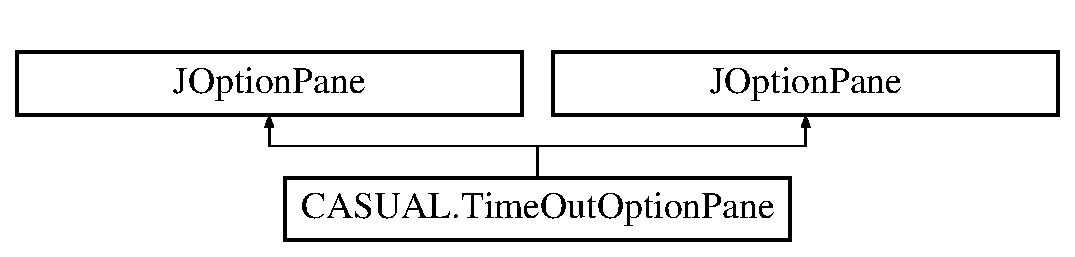
\includegraphics[height=2.000000cm]{classCASUAL_1_1TimeOutOptionPane}
\end{center}
\end{figure}
\subsection*{Public Member Functions}
\begin{DoxyCompactItemize}
\item 
\hypertarget{classCASUAL_1_1TimeOutOptionPane_aab8afad966d7fbb21ab8478b4b7f61b5}{int {\bfseries show\-Timeout\-Dialog} (final int P\-R\-E\-S\-E\-T\-\_\-\-T\-I\-M\-E, Component parent\-Component, Object message, final String title, int option\-Type, int message\-Type, Object\mbox{[}$\,$\mbox{]} options, final Object initial\-Value)}\label{classCASUAL_1_1TimeOutOptionPane_aab8afad966d7fbb21ab8478b4b7f61b5}

\item 
\hypertarget{classCASUAL_1_1TimeOutOptionPane_aab8afad966d7fbb21ab8478b4b7f61b5}{int {\bfseries show\-Timeout\-Dialog} (final int P\-R\-E\-S\-E\-T\-\_\-\-T\-I\-M\-E, Component parent\-Component, Object message, final String title, int option\-Type, int message\-Type, Object\mbox{[}$\,$\mbox{]} options, final Object initial\-Value)}\label{classCASUAL_1_1TimeOutOptionPane_aab8afad966d7fbb21ab8478b4b7f61b5}

\end{DoxyCompactItemize}


\subsection{Detailed Description}
\begin{DoxyAuthor}{Author}
adam 
\end{DoxyAuthor}


The documentation for this class was generated from the following files\-:\begin{DoxyCompactItemize}
\item 
branches/\-C\-A\-S\-U\-A\-L-\/\-Headless/\-G\-U\-I/src/\-C\-A\-S\-U\-A\-L/Time\-Out\-Option\-Pane.\-java\item 
branches/\-Testing\-Branch/\-G\-Doc/src/\-C\-A\-S\-U\-A\-L/Time\-Out\-Option\-Pane.\-java\end{DoxyCompactItemize}

\hypertarget{classGUI_1_1development_1_1TimeOutOptionPane}{\section{G\-U\-I.\-development.\-Time\-Out\-Option\-Pane Class Reference}
\label{classGUI_1_1development_1_1TimeOutOptionPane}\index{G\-U\-I.\-development.\-Time\-Out\-Option\-Pane@{G\-U\-I.\-development.\-Time\-Out\-Option\-Pane}}
}
Inheritance diagram for G\-U\-I.\-development.\-Time\-Out\-Option\-Pane\-:\begin{figure}[H]
\begin{center}
\leavevmode
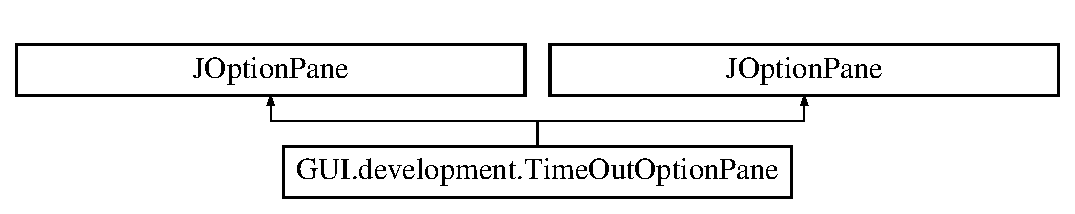
\includegraphics[height=2.000000cm]{classGUI_1_1development_1_1TimeOutOptionPane}
\end{center}
\end{figure}
\subsection*{Public Member Functions}
\begin{DoxyCompactItemize}
\item 
\hyperlink{classGUI_1_1development_1_1TimeOutOptionPane_accd0bbe0a3a759e4f0b31c2a61ece537}{Time\-Out\-Option\-Pane} ()
\item 
int \hyperlink{classGUI_1_1development_1_1TimeOutOptionPane_a76d2a6139406a26514ce249b41e4e748}{timeout\-Dialog} (final int time, Component parent\-Component, Object message, final String title, int option\-Type, int message\-Type, Object\mbox{[}$\,$\mbox{]} options, final Object initial\-Value)
\item 
\hyperlink{classGUI_1_1development_1_1TimeOutOptionPane_accd0bbe0a3a759e4f0b31c2a61ece537}{Time\-Out\-Option\-Pane} ()
\item 
int \hyperlink{classGUI_1_1development_1_1TimeOutOptionPane_a76d2a6139406a26514ce249b41e4e748}{timeout\-Dialog} (final int time, Component parent\-Component, Object message, final String title, int option\-Type, int message\-Type, Object\mbox{[}$\,$\mbox{]} options, final Object initial\-Value)
\end{DoxyCompactItemize}


\subsection{Detailed Description}
\begin{DoxyAuthor}{Author}
adam 
\end{DoxyAuthor}


\subsection{Constructor \& Destructor Documentation}
\hypertarget{classGUI_1_1development_1_1TimeOutOptionPane_accd0bbe0a3a759e4f0b31c2a61ece537}{\index{G\-U\-I\-::development\-::\-Time\-Out\-Option\-Pane@{G\-U\-I\-::development\-::\-Time\-Out\-Option\-Pane}!Time\-Out\-Option\-Pane@{Time\-Out\-Option\-Pane}}
\index{Time\-Out\-Option\-Pane@{Time\-Out\-Option\-Pane}!GUI::development::TimeOutOptionPane@{G\-U\-I\-::development\-::\-Time\-Out\-Option\-Pane}}
\subsubsection[{Time\-Out\-Option\-Pane}]{\setlength{\rightskip}{0pt plus 5cm}G\-U\-I.\-development.\-Time\-Out\-Option\-Pane.\-Time\-Out\-Option\-Pane (
\begin{DoxyParamCaption}
{}
\end{DoxyParamCaption}
)}}\label{classGUI_1_1development_1_1TimeOutOptionPane_accd0bbe0a3a759e4f0b31c2a61ece537}
instantiates a timeout option pane \hypertarget{classGUI_1_1development_1_1TimeOutOptionPane_accd0bbe0a3a759e4f0b31c2a61ece537}{\index{G\-U\-I\-::development\-::\-Time\-Out\-Option\-Pane@{G\-U\-I\-::development\-::\-Time\-Out\-Option\-Pane}!Time\-Out\-Option\-Pane@{Time\-Out\-Option\-Pane}}
\index{Time\-Out\-Option\-Pane@{Time\-Out\-Option\-Pane}!GUI::development::TimeOutOptionPane@{G\-U\-I\-::development\-::\-Time\-Out\-Option\-Pane}}
\subsubsection[{Time\-Out\-Option\-Pane}]{\setlength{\rightskip}{0pt plus 5cm}G\-U\-I.\-development.\-Time\-Out\-Option\-Pane.\-Time\-Out\-Option\-Pane (
\begin{DoxyParamCaption}
{}
\end{DoxyParamCaption}
)}}\label{classGUI_1_1development_1_1TimeOutOptionPane_accd0bbe0a3a759e4f0b31c2a61ece537}
instantiates a timeout option pane 

\subsection{Member Function Documentation}
\hypertarget{classGUI_1_1development_1_1TimeOutOptionPane_a76d2a6139406a26514ce249b41e4e748}{\index{G\-U\-I\-::development\-::\-Time\-Out\-Option\-Pane@{G\-U\-I\-::development\-::\-Time\-Out\-Option\-Pane}!timeout\-Dialog@{timeout\-Dialog}}
\index{timeout\-Dialog@{timeout\-Dialog}!GUI::development::TimeOutOptionPane@{G\-U\-I\-::development\-::\-Time\-Out\-Option\-Pane}}
\subsubsection[{timeout\-Dialog}]{\setlength{\rightskip}{0pt plus 5cm}int G\-U\-I.\-development.\-Time\-Out\-Option\-Pane.\-timeout\-Dialog (
\begin{DoxyParamCaption}
\item[{final int}]{time, }
\item[{Component}]{parent\-Component, }
\item[{Object}]{message, }
\item[{final String}]{title, }
\item[{int}]{option\-Type, }
\item[{int}]{message\-Type, }
\item[{Object\mbox{[}$\,$\mbox{]}}]{options, }
\item[{final Object}]{initial\-Value}
\end{DoxyParamCaption}
)}}\label{classGUI_1_1development_1_1TimeOutOptionPane_a76d2a6139406a26514ce249b41e4e748}
timeout option pane 
\begin{DoxyParams}{Parameters}
{\em time} & time limit to wait \\
\hline
{\em parent\-Component} & display over \\
\hline
{\em message} & message to be displayed \\
\hline
{\em title} & title of message \\
\hline
{\em option\-Type} & J\-Option\-Pane.\-O\-P\-T\-I\-O\-N \\
\hline
{\em message\-Type} & J\-Option\-Pane.\-T\-Y\-P\-E \\
\hline
{\em options} & button values \\
\hline
{\em initial\-Value} & default value to select if time runs out \\
\hline
\end{DoxyParams}
\begin{DoxyReturn}{Returns}
integer representing user selection 
\end{DoxyReturn}
\hypertarget{classGUI_1_1development_1_1TimeOutOptionPane_a76d2a6139406a26514ce249b41e4e748}{\index{G\-U\-I\-::development\-::\-Time\-Out\-Option\-Pane@{G\-U\-I\-::development\-::\-Time\-Out\-Option\-Pane}!timeout\-Dialog@{timeout\-Dialog}}
\index{timeout\-Dialog@{timeout\-Dialog}!GUI::development::TimeOutOptionPane@{G\-U\-I\-::development\-::\-Time\-Out\-Option\-Pane}}
\subsubsection[{timeout\-Dialog}]{\setlength{\rightskip}{0pt plus 5cm}int G\-U\-I.\-development.\-Time\-Out\-Option\-Pane.\-timeout\-Dialog (
\begin{DoxyParamCaption}
\item[{final int}]{time, }
\item[{Component}]{parent\-Component, }
\item[{Object}]{message, }
\item[{final String}]{title, }
\item[{int}]{option\-Type, }
\item[{int}]{message\-Type, }
\item[{Object\mbox{[}$\,$\mbox{]}}]{options, }
\item[{final Object}]{initial\-Value}
\end{DoxyParamCaption}
)}}\label{classGUI_1_1development_1_1TimeOutOptionPane_a76d2a6139406a26514ce249b41e4e748}
timeout option pane 
\begin{DoxyParams}{Parameters}
{\em time} & time limit to wait \\
\hline
{\em parent\-Component} & display over \\
\hline
{\em message} & message to be displayed \\
\hline
{\em title} & title of message \\
\hline
{\em option\-Type} & J\-Option\-Pane.\-O\-P\-T\-I\-O\-N \\
\hline
{\em message\-Type} & J\-Option\-Pane.\-T\-Y\-P\-E \\
\hline
{\em options} & button values \\
\hline
{\em initial\-Value} & default value to select if time runs out \\
\hline
\end{DoxyParams}
\begin{DoxyReturn}{Returns}
integer representing user selection 
\end{DoxyReturn}


The documentation for this class was generated from the following files\-:\begin{DoxyCompactItemize}
\item 
trunk/\-C\-A\-S\-U\-A\-Lcore/build/classes/\-G\-U\-I/development/Time\-Out\-Option\-Pane.\-java\item 
trunk/\-C\-A\-S\-U\-A\-Lcore/src/\-G\-U\-I/development/Time\-Out\-Option\-Pane.\-java\end{DoxyCompactItemize}

\hypertarget{classCASUAL_1_1Translations}{\section{C\-A\-S\-U\-A\-L.\-Translations Class Reference}
\label{classCASUAL_1_1Translations}\index{C\-A\-S\-U\-A\-L.\-Translations@{C\-A\-S\-U\-A\-L.\-Translations}}
}
\subsection*{Public Member Functions}
\begin{DoxyCompactItemize}
\item 
void \hyperlink{classCASUAL_1_1Translations_a76d82a376b36383cb77f7e445006315c}{set\-Language} (String lang)
\end{DoxyCompactItemize}
\subsection*{Static Public Member Functions}
\begin{DoxyCompactItemize}
\item 
static String \hyperlink{classCASUAL_1_1Translations_a75aaa59b24f56ac6eb9fb47879a9cd6e}{get} (String line)
\end{DoxyCompactItemize}


\subsection{Detailed Description}
\begin{DoxyAuthor}{Author}
adam 
\end{DoxyAuthor}


\subsection{Member Function Documentation}
\hypertarget{classCASUAL_1_1Translations_a75aaa59b24f56ac6eb9fb47879a9cd6e}{\index{C\-A\-S\-U\-A\-L\-::\-Translations@{C\-A\-S\-U\-A\-L\-::\-Translations}!get@{get}}
\index{get@{get}!CASUAL::Translations@{C\-A\-S\-U\-A\-L\-::\-Translations}}
\subsubsection[{get}]{\setlength{\rightskip}{0pt plus 5cm}static String C\-A\-S\-U\-A\-L.\-Translations.\-get (
\begin{DoxyParamCaption}
\item[{String}]{line}
\end{DoxyParamCaption}
)\hspace{0.3cm}{\ttfamily [static]}}}\label{classCASUAL_1_1Translations_a75aaa59b24f56ac6eb9fb47879a9cd6e}
Returns translated string from translation Resource Bundle. Checks to make sure there is a valid resource file. Default locale is loaded if required. The input String is split by \char`\"{} \char`\"{} and \char`\"{}\textbackslash{}n\char`\"{}. If the split values start with the (at) character, a translation is attempted.


\begin{DoxyParams}{Parameters}
{\em line} & string to be translated \\
\hline
\end{DoxyParams}
\begin{DoxyReturn}{Returns}
translated line 
\end{DoxyReturn}
\hypertarget{classCASUAL_1_1Translations_a76d82a376b36383cb77f7e445006315c}{\index{C\-A\-S\-U\-A\-L\-::\-Translations@{C\-A\-S\-U\-A\-L\-::\-Translations}!set\-Language@{set\-Language}}
\index{set\-Language@{set\-Language}!CASUAL::Translations@{C\-A\-S\-U\-A\-L\-::\-Translations}}
\subsubsection[{set\-Language}]{\setlength{\rightskip}{0pt plus 5cm}void C\-A\-S\-U\-A\-L.\-Translations.\-set\-Language (
\begin{DoxyParamCaption}
\item[{String}]{lang}
\end{DoxyParamCaption}
)}}\label{classCASUAL_1_1Translations_a76d82a376b36383cb77f7e445006315c}
Sets up a translation language for testing \hyperlink{namespaceCASUAL}{C\-A\-S\-U\-A\-L}. If the translation is missing, the default is C\-A\-S\-U\-A\-L/resources/\-Translations/\-English.\-properties.


\begin{DoxyParams}{Parameters}
{\em lang} & attempts to load specified language. \\
\hline
\end{DoxyParams}


The documentation for this class was generated from the following file\-:\begin{DoxyCompactItemize}
\item 
trunk/\-C\-A\-S\-U\-A\-Lcore/src/\-C\-A\-S\-U\-A\-L/Translations.\-java\end{DoxyCompactItemize}

\hypertarget{classCASUAL_1_1TranslationsTest}{\section{C\-A\-S\-U\-A\-L.\-Translations\-Test Class Reference}
\label{classCASUAL_1_1TranslationsTest}\index{C\-A\-S\-U\-A\-L.\-Translations\-Test@{C\-A\-S\-U\-A\-L.\-Translations\-Test}}
}
\subsection*{Public Member Functions}
\begin{DoxyCompactItemize}
\item 
\hypertarget{classCASUAL_1_1TranslationsTest_a7a0fd0a580f7479985835b31c4693fb4}{void {\bfseries translation1} ()}\label{classCASUAL_1_1TranslationsTest_a7a0fd0a580f7479985835b31c4693fb4}

\end{DoxyCompactItemize}
\subsection*{Static Public Member Functions}
\begin{DoxyCompactItemize}
\item 
\hypertarget{classCASUAL_1_1TranslationsTest_a996baecd9242ec89d7907086b88257dc}{static void {\bfseries set\-Up\-Class} ()}\label{classCASUAL_1_1TranslationsTest_a996baecd9242ec89d7907086b88257dc}

\item 
\hypertarget{classCASUAL_1_1TranslationsTest_a2642ae0a02b26ffa5b222025f85f9be2}{static void {\bfseries tear\-Down\-Class} ()}\label{classCASUAL_1_1TranslationsTest_a2642ae0a02b26ffa5b222025f85f9be2}

\end{DoxyCompactItemize}


\subsection{Detailed Description}
\begin{DoxyAuthor}{Author}
adamoutler 
\end{DoxyAuthor}


The documentation for this class was generated from the following file\-:\begin{DoxyCompactItemize}
\item 
trunk/\-C\-A\-S\-U\-A\-Lcore/test/\-C\-A\-S\-U\-A\-L/Translations\-Test.\-java\end{DoxyCompactItemize}

\hypertarget{classCASUAL_1_1Unzip}{\section{C\-A\-S\-U\-A\-L.\-Unzip Class Reference}
\label{classCASUAL_1_1Unzip}\index{C\-A\-S\-U\-A\-L.\-Unzip@{C\-A\-S\-U\-A\-L.\-Unzip}}
}
\subsection*{Public Member Functions}
\begin{DoxyCompactItemize}
\item 
\hypertarget{classCASUAL_1_1Unzip_a663c2348804e17be43f339e596f76b22}{void {\bfseries unzip\-Files} ()}\label{classCASUAL_1_1Unzip_a663c2348804e17be43f339e596f76b22}

\item 
\hypertarget{classCASUAL_1_1Unzip_a7f8c9c77edbb7b07afec4c6a8d6f2060}{void {\bfseries unzip\-File} (String zip\-File, String Output\-Folder)  throws Zip\-Exception, I\-O\-Exception }\label{classCASUAL_1_1Unzip_a7f8c9c77edbb7b07afec4c6a8d6f2060}

\item 
\hypertarget{classCASUAL_1_1Unzip_ae5d9c021b1d4b4a27b408b3bbd1a44e6}{void {\bfseries Un\-Zip\-Resource} (String Zip\-Resource, String Output\-Folder)  throws File\-Not\-Found\-Exception, I\-O\-Exception }\label{classCASUAL_1_1Unzip_ae5d9c021b1d4b4a27b408b3bbd1a44e6}

\item 
\hypertarget{classCASUAL_1_1Unzip_a663c2348804e17be43f339e596f76b22}{void {\bfseries unzip\-Files} ()}\label{classCASUAL_1_1Unzip_a663c2348804e17be43f339e596f76b22}

\item 
\hypertarget{classCASUAL_1_1Unzip_a7f8c9c77edbb7b07afec4c6a8d6f2060}{void {\bfseries unzip\-File} (String zip\-File, String Output\-Folder)  throws Zip\-Exception, I\-O\-Exception }\label{classCASUAL_1_1Unzip_a7f8c9c77edbb7b07afec4c6a8d6f2060}

\item 
\hypertarget{classCASUAL_1_1Unzip_ae5d9c021b1d4b4a27b408b3bbd1a44e6}{void {\bfseries Un\-Zip\-Resource} (String Zip\-Resource, String Output\-Folder)  throws File\-Not\-Found\-Exception, I\-O\-Exception }\label{classCASUAL_1_1Unzip_ae5d9c021b1d4b4a27b408b3bbd1a44e6}

\end{DoxyCompactItemize}


\subsection{Detailed Description}
\begin{DoxyAuthor}{Author}
adam 
\end{DoxyAuthor}


The documentation for this class was generated from the following files\-:\begin{DoxyCompactItemize}
\item 
branches/\-C\-A\-S\-U\-A\-L-\/\-Headless/\-G\-U\-I/src/\-C\-A\-S\-U\-A\-L/Unzip.\-java\item 
branches/\-Testing\-Branch/\-G\-Doc/src/\-C\-A\-S\-U\-A\-L/Unzip.\-java\end{DoxyCompactItemize}

\hypertarget{classCASUAL_1_1archiving_1_1Unzip}{\section{C\-A\-S\-U\-A\-L.\-archiving.\-Unzip Class Reference}
\label{classCASUAL_1_1archiving_1_1Unzip}\index{C\-A\-S\-U\-A\-L.\-archiving.\-Unzip@{C\-A\-S\-U\-A\-L.\-archiving.\-Unzip}}
}
\subsection*{Public Member Functions}
\begin{DoxyCompactItemize}
\item 
\hyperlink{classCASUAL_1_1archiving_1_1Unzip_a88ff2e111af2352f8101ea87acc2d6d4}{Unzip} (File f)  throws Zip\-Exception, I\-O\-Exception 
\item 
\hyperlink{classCASUAL_1_1archiving_1_1Unzip_abc708c4bf25ed0e0edeabf0c71bbd344}{Unzip} (String f)  throws Zip\-Exception, I\-O\-Exception 
\item 
void \hyperlink{classCASUAL_1_1archiving_1_1Unzip_a477d977d8734e6064cc41cd8acc005a9}{unzip\-File} (String output\-Folder)  throws Zip\-Exception, I\-O\-Exception 
\item 
void \hyperlink{classCASUAL_1_1archiving_1_1Unzip_a14b0d899780a66d69b01ac7034d4a90e}{close} ()
\item 
String \hyperlink{classCASUAL_1_1archiving_1_1Unzip_a568a39dbfeb9064924d41b441da6e454}{deploy\-File\-From\-Zip} (Object entry, String output\-Folder)  throws Zip\-Exception, I\-O\-Exception 
\item 
Buffered\-Input\-Stream \hyperlink{classCASUAL_1_1archiving_1_1Unzip_a285658d9e0121e2859a2c35600a0c9d0}{stream\-File\-From\-Zip} (Object entry)  throws Zip\-Exception, I\-O\-Exception 
\item 
String \hyperlink{classCASUAL_1_1archiving_1_1Unzip_a750b1ed907dfd4da6931289e53094754}{get\-Entry\-Name} (Object entry)
\item 
Zip\-Entry \hyperlink{classCASUAL_1_1archiving_1_1Unzip_aebf6db26bcbca3b4f76833f8372c6302}{get\-Entry} (Object entry)
\end{DoxyCompactItemize}
\subsection*{Static Public Member Functions}
\begin{DoxyCompactItemize}
\item 
static void \hyperlink{classCASUAL_1_1archiving_1_1Unzip_a20374a024e3d57ee34f7d2f1f6e79e6f}{un\-Zip\-Resource} (String zip\-Resource, String output\-Folder)  throws File\-Not\-Found\-Exception, I\-O\-Exception 
\item 
static void \hyperlink{classCASUAL_1_1archiving_1_1Unzip_ac13b6d000c8747a6d73874cc7c95bfa8}{un\-Zip\-Input\-Stream} (Input\-Stream z\-Stream, String output\-Folder)  throws File\-Not\-Found\-Exception, I\-O\-Exception 
\item 
static Buffered\-Input\-Stream \hyperlink{classCASUAL_1_1archiving_1_1Unzip_a040693a39393fa52d90c18180f7543ea}{stream\-File\-From\-Zip} (File zip\-File, Object entry)  throws Zip\-Exception, I\-O\-Exception 
\end{DoxyCompactItemize}
\subsection*{Public Attributes}
\begin{DoxyCompactItemize}
\item 
Enumeration$<$?extends Zip\-Entry $>$ \hyperlink{classCASUAL_1_1archiving_1_1Unzip_a9baca609154eb94b13e456d523d17eab}{zip\-File\-Entries}
\end{DoxyCompactItemize}


\subsection{Detailed Description}
\begin{DoxyAuthor}{Author}
adam 
\end{DoxyAuthor}


\subsection{Constructor \& Destructor Documentation}
\hypertarget{classCASUAL_1_1archiving_1_1Unzip_a88ff2e111af2352f8101ea87acc2d6d4}{\index{C\-A\-S\-U\-A\-L\-::archiving\-::\-Unzip@{C\-A\-S\-U\-A\-L\-::archiving\-::\-Unzip}!Unzip@{Unzip}}
\index{Unzip@{Unzip}!CASUAL::archiving::Unzip@{C\-A\-S\-U\-A\-L\-::archiving\-::\-Unzip}}
\subsubsection[{Unzip}]{\setlength{\rightskip}{0pt plus 5cm}C\-A\-S\-U\-A\-L.\-archiving.\-Unzip.\-Unzip (
\begin{DoxyParamCaption}
\item[{File}]{f}
\end{DoxyParamCaption}
) throws Zip\-Exception, I\-O\-Exception}}\label{classCASUAL_1_1archiving_1_1Unzip_a88ff2e111af2352f8101ea87acc2d6d4}
\hyperlink{classCASUAL_1_1archiving_1_1Unzip}{Unzip} class is used to create a wrapper for unziping .zip files. 

The File f will be converted to a Zip\-File, and all other operations will be preformed on this Zip\-File.


\begin{DoxyParams}{Parameters}
{\em f} & java file object to be unziped. \\
\hline
\end{DoxyParams}

\begin{DoxyExceptions}{Exceptions}
{\em Zip\-Exception} & \\
\hline
{\em I\-O\-Exception} & \\
\hline
\end{DoxyExceptions}
\begin{DoxySeeAlso}{See Also}
Zip\-File 
\end{DoxySeeAlso}
\hypertarget{classCASUAL_1_1archiving_1_1Unzip_abc708c4bf25ed0e0edeabf0c71bbd344}{\index{C\-A\-S\-U\-A\-L\-::archiving\-::\-Unzip@{C\-A\-S\-U\-A\-L\-::archiving\-::\-Unzip}!Unzip@{Unzip}}
\index{Unzip@{Unzip}!CASUAL::archiving::Unzip@{C\-A\-S\-U\-A\-L\-::archiving\-::\-Unzip}}
\subsubsection[{Unzip}]{\setlength{\rightskip}{0pt plus 5cm}C\-A\-S\-U\-A\-L.\-archiving.\-Unzip.\-Unzip (
\begin{DoxyParamCaption}
\item[{String}]{f}
\end{DoxyParamCaption}
) throws Zip\-Exception, I\-O\-Exception}}\label{classCASUAL_1_1archiving_1_1Unzip_abc708c4bf25ed0e0edeabf0c71bbd344}
\hyperlink{classCASUAL_1_1archiving_1_1Unzip}{Unzip} class is used to create a wrapper for unziping .zip files. 

The String f will be converted into a file, then that file will be converted into a Zip\-File.


\begin{DoxyParams}{Parameters}
{\em f} & String location of file to be unziped. \\
\hline
\end{DoxyParams}

\begin{DoxyExceptions}{Exceptions}
{\em Zip\-Exception} & \\
\hline
{\em I\-O\-Exception} & \\
\hline
\end{DoxyExceptions}
\begin{DoxySeeAlso}{See Also}
Zip\-File 
\end{DoxySeeAlso}


\subsection{Member Function Documentation}
\hypertarget{classCASUAL_1_1archiving_1_1Unzip_a14b0d899780a66d69b01ac7034d4a90e}{\index{C\-A\-S\-U\-A\-L\-::archiving\-::\-Unzip@{C\-A\-S\-U\-A\-L\-::archiving\-::\-Unzip}!close@{close}}
\index{close@{close}!CASUAL::archiving::Unzip@{C\-A\-S\-U\-A\-L\-::archiving\-::\-Unzip}}
\subsubsection[{close}]{\setlength{\rightskip}{0pt plus 5cm}void C\-A\-S\-U\-A\-L.\-archiving.\-Unzip.\-close (
\begin{DoxyParamCaption}
{}
\end{DoxyParamCaption}
)}}\label{classCASUAL_1_1archiving_1_1Unzip_a14b0d899780a66d69b01ac7034d4a90e}
Closes the zip file 

Should be called after all file operations have been completed in \hyperlink{classCASUAL_1_1archiving_1_1Unzip}{Unzip} \hypertarget{classCASUAL_1_1archiving_1_1Unzip_a568a39dbfeb9064924d41b441da6e454}{\index{C\-A\-S\-U\-A\-L\-::archiving\-::\-Unzip@{C\-A\-S\-U\-A\-L\-::archiving\-::\-Unzip}!deploy\-File\-From\-Zip@{deploy\-File\-From\-Zip}}
\index{deploy\-File\-From\-Zip@{deploy\-File\-From\-Zip}!CASUAL::archiving::Unzip@{C\-A\-S\-U\-A\-L\-::archiving\-::\-Unzip}}
\subsubsection[{deploy\-File\-From\-Zip}]{\setlength{\rightskip}{0pt plus 5cm}String C\-A\-S\-U\-A\-L.\-archiving.\-Unzip.\-deploy\-File\-From\-Zip (
\begin{DoxyParamCaption}
\item[{Object}]{entry, }
\item[{String}]{output\-Folder}
\end{DoxyParamCaption}
) throws Zip\-Exception, I\-O\-Exception}}\label{classCASUAL_1_1archiving_1_1Unzip_a568a39dbfeb9064924d41b441da6e454}
Deploys a single file from a zip. 

Takes in an Zip\-Entry, and writes that single zip entry out to a folder


\begin{DoxyParams}{Parameters}
{\em entry} & entry file to deploy \\
\hline
{\em output\-Folder} & folder to be deployed to \\
\hline
\end{DoxyParams}
\begin{DoxyReturn}{Returns}
location of entry deployed 
\end{DoxyReturn}

\begin{DoxyExceptions}{Exceptions}
{\em Zip\-Exception} & \\
\hline
{\em I\-O\-Exception} & \\
\hline
\end{DoxyExceptions}
\hypertarget{classCASUAL_1_1archiving_1_1Unzip_aebf6db26bcbca3b4f76833f8372c6302}{\index{C\-A\-S\-U\-A\-L\-::archiving\-::\-Unzip@{C\-A\-S\-U\-A\-L\-::archiving\-::\-Unzip}!get\-Entry@{get\-Entry}}
\index{get\-Entry@{get\-Entry}!CASUAL::archiving::Unzip@{C\-A\-S\-U\-A\-L\-::archiving\-::\-Unzip}}
\subsubsection[{get\-Entry}]{\setlength{\rightskip}{0pt plus 5cm}Zip\-Entry C\-A\-S\-U\-A\-L.\-archiving.\-Unzip.\-get\-Entry (
\begin{DoxyParamCaption}
\item[{Object}]{entry}
\end{DoxyParamCaption}
)}}\label{classCASUAL_1_1archiving_1_1Unzip_aebf6db26bcbca3b4f76833f8372c6302}
Takes in an Zip\-Entry as an object and returns the Zip\-Entry for the Object.


\begin{DoxyParams}{Parameters}
{\em entry} & the Zip\-Entry Object \\
\hline
\end{DoxyParams}
\begin{DoxyReturn}{Returns}
the Zip\-Entry 
\end{DoxyReturn}
\begin{DoxySeeAlso}{See Also}
Zip\-Entry 
\end{DoxySeeAlso}
\hypertarget{classCASUAL_1_1archiving_1_1Unzip_a750b1ed907dfd4da6931289e53094754}{\index{C\-A\-S\-U\-A\-L\-::archiving\-::\-Unzip@{C\-A\-S\-U\-A\-L\-::archiving\-::\-Unzip}!get\-Entry\-Name@{get\-Entry\-Name}}
\index{get\-Entry\-Name@{get\-Entry\-Name}!CASUAL::archiving::Unzip@{C\-A\-S\-U\-A\-L\-::archiving\-::\-Unzip}}
\subsubsection[{get\-Entry\-Name}]{\setlength{\rightskip}{0pt plus 5cm}String C\-A\-S\-U\-A\-L.\-archiving.\-Unzip.\-get\-Entry\-Name (
\begin{DoxyParamCaption}
\item[{Object}]{entry}
\end{DoxyParamCaption}
)}}\label{classCASUAL_1_1archiving_1_1Unzip_a750b1ed907dfd4da6931289e53094754}
Takes in a Zip\-Entry as an object and returns the string of the corresponding file name for the entry.


\begin{DoxyParams}{Parameters}
{\em entry} & the Zip\-Entry Object \\
\hline
\end{DoxyParams}
\begin{DoxyReturn}{Returns}
name of the file contained in the 
\end{DoxyReturn}
\begin{DoxySeeAlso}{See Also}
Zip\-Entry\-::get\-Name() 
\end{DoxySeeAlso}
\hypertarget{classCASUAL_1_1archiving_1_1Unzip_a040693a39393fa52d90c18180f7543ea}{\index{C\-A\-S\-U\-A\-L\-::archiving\-::\-Unzip@{C\-A\-S\-U\-A\-L\-::archiving\-::\-Unzip}!stream\-File\-From\-Zip@{stream\-File\-From\-Zip}}
\index{stream\-File\-From\-Zip@{stream\-File\-From\-Zip}!CASUAL::archiving::Unzip@{C\-A\-S\-U\-A\-L\-::archiving\-::\-Unzip}}
\subsubsection[{stream\-File\-From\-Zip}]{\setlength{\rightskip}{0pt plus 5cm}static Buffered\-Input\-Stream C\-A\-S\-U\-A\-L.\-archiving.\-Unzip.\-stream\-File\-From\-Zip (
\begin{DoxyParamCaption}
\item[{File}]{zip\-File, }
\item[{Object}]{entry}
\end{DoxyParamCaption}
) throws Zip\-Exception, I\-O\-Exception\hspace{0.3cm}{\ttfamily [static]}}}\label{classCASUAL_1_1archiving_1_1Unzip_a040693a39393fa52d90c18180f7543ea}
Gets a stream of a specified file from a zip. 

Static method used to stream a file form a zip that is not an \hyperlink{classCASUAL_1_1archiving_1_1Unzip}{Unzip} object.


\begin{DoxyParams}{Parameters}
{\em zip\-File} & file to stream from \\
\hline
{\em entry} & entry to stream \\
\hline
\end{DoxyParams}
\begin{DoxyReturn}{Returns}
stream of file 
\end{DoxyReturn}

\begin{DoxyExceptions}{Exceptions}
{\em Zip\-Exception} & \\
\hline
{\em I\-O\-Exception} & \\
\hline
\end{DoxyExceptions}
\hypertarget{classCASUAL_1_1archiving_1_1Unzip_a285658d9e0121e2859a2c35600a0c9d0}{\index{C\-A\-S\-U\-A\-L\-::archiving\-::\-Unzip@{C\-A\-S\-U\-A\-L\-::archiving\-::\-Unzip}!stream\-File\-From\-Zip@{stream\-File\-From\-Zip}}
\index{stream\-File\-From\-Zip@{stream\-File\-From\-Zip}!CASUAL::archiving::Unzip@{C\-A\-S\-U\-A\-L\-::archiving\-::\-Unzip}}
\subsubsection[{stream\-File\-From\-Zip}]{\setlength{\rightskip}{0pt plus 5cm}Buffered\-Input\-Stream C\-A\-S\-U\-A\-L.\-archiving.\-Unzip.\-stream\-File\-From\-Zip (
\begin{DoxyParamCaption}
\item[{Object}]{entry}
\end{DoxyParamCaption}
) throws Zip\-Exception, I\-O\-Exception}}\label{classCASUAL_1_1archiving_1_1Unzip_a285658d9e0121e2859a2c35600a0c9d0}
Retrieves a Buffered\-Input\-Stream for a specific zip entry in a file.


\begin{DoxyParams}{Parameters}
{\em entry} & Zip\-Entry that is to be pulled from Zip\-File to Stream. \\
\hline
\end{DoxyParams}
\begin{DoxyReturn}{Returns}
Buffered\-Input\-Stream of the specified Zip\-Entry. 
\end{DoxyReturn}

\begin{DoxyExceptions}{Exceptions}
{\em Zip\-Exception} & \\
\hline
{\em I\-O\-Exception} & \\
\hline
\end{DoxyExceptions}
\begin{DoxySeeAlso}{See Also}
Zip\-Entry 

Zip\-File 

Buffered\-Input\-Stream 
\end{DoxySeeAlso}
\hypertarget{classCASUAL_1_1archiving_1_1Unzip_a477d977d8734e6064cc41cd8acc005a9}{\index{C\-A\-S\-U\-A\-L\-::archiving\-::\-Unzip@{C\-A\-S\-U\-A\-L\-::archiving\-::\-Unzip}!unzip\-File@{unzip\-File}}
\index{unzip\-File@{unzip\-File}!CASUAL::archiving::Unzip@{C\-A\-S\-U\-A\-L\-::archiving\-::\-Unzip}}
\subsubsection[{unzip\-File}]{\setlength{\rightskip}{0pt plus 5cm}void C\-A\-S\-U\-A\-L.\-archiving.\-Unzip.\-unzip\-File (
\begin{DoxyParamCaption}
\item[{String}]{output\-Folder}
\end{DoxyParamCaption}
) throws Zip\-Exception, I\-O\-Exception}}\label{classCASUAL_1_1archiving_1_1Unzip_a477d977d8734e6064cc41cd8acc005a9}
Unzips the Zip\-File that was specified in the constructor of the class.


\begin{DoxyParams}{Parameters}
{\em output\-Folder} & folder to be unzipped to \\
\hline
\end{DoxyParams}

\begin{DoxyExceptions}{Exceptions}
{\em Zip\-Exception} & \\
\hline
{\em I\-O\-Exception} & \\
\hline
\end{DoxyExceptions}
\begin{DoxySeeAlso}{See Also}
\hyperlink{classCASUAL_1_1archiving_1_1Unzip_a88ff2e111af2352f8101ea87acc2d6d4}{C\-A\-S\-U\-A\-L.\-archiving.\-Unzip\-::\-Unzip(\-File)} 
\end{DoxySeeAlso}
\hypertarget{classCASUAL_1_1archiving_1_1Unzip_ac13b6d000c8747a6d73874cc7c95bfa8}{\index{C\-A\-S\-U\-A\-L\-::archiving\-::\-Unzip@{C\-A\-S\-U\-A\-L\-::archiving\-::\-Unzip}!un\-Zip\-Input\-Stream@{un\-Zip\-Input\-Stream}}
\index{un\-Zip\-Input\-Stream@{un\-Zip\-Input\-Stream}!CASUAL::archiving::Unzip@{C\-A\-S\-U\-A\-L\-::archiving\-::\-Unzip}}
\subsubsection[{un\-Zip\-Input\-Stream}]{\setlength{\rightskip}{0pt plus 5cm}static void C\-A\-S\-U\-A\-L.\-archiving.\-Unzip.\-un\-Zip\-Input\-Stream (
\begin{DoxyParamCaption}
\item[{Input\-Stream}]{z\-Stream, }
\item[{String}]{output\-Folder}
\end{DoxyParamCaption}
) throws File\-Not\-Found\-Exception, I\-O\-Exception\hspace{0.3cm}{\ttfamily [static]}}}\label{classCASUAL_1_1archiving_1_1Unzip_ac13b6d000c8747a6d73874cc7c95bfa8}
Unzips an Input\-Stream. 

Takes in an Input\-Stream, converts it to a Zip\-Input\-Stream, and then iterates through all of the Zip\-Entries, writing each one of them to a file with the name provided by the Zip\-Entry.


\begin{DoxyParams}{Parameters}
{\em z\-Stream} & input stream to unzip \\
\hline
{\em output\-Folder} & output folder to unzip to \\
\hline
\end{DoxyParams}

\begin{DoxyExceptions}{Exceptions}
{\em File\-Not\-Found\-Exception} & \\
\hline
{\em I\-O\-Exception} & \\
\hline
\end{DoxyExceptions}
\begin{DoxySeeAlso}{See Also}
Input\-Stream 

Zip\-Entry 

Zip\-Input\-Stream 

Zip\-File 
\end{DoxySeeAlso}
\hypertarget{classCASUAL_1_1archiving_1_1Unzip_a20374a024e3d57ee34f7d2f1f6e79e6f}{\index{C\-A\-S\-U\-A\-L\-::archiving\-::\-Unzip@{C\-A\-S\-U\-A\-L\-::archiving\-::\-Unzip}!un\-Zip\-Resource@{un\-Zip\-Resource}}
\index{un\-Zip\-Resource@{un\-Zip\-Resource}!CASUAL::archiving::Unzip@{C\-A\-S\-U\-A\-L\-::archiving\-::\-Unzip}}
\subsubsection[{un\-Zip\-Resource}]{\setlength{\rightskip}{0pt plus 5cm}static void C\-A\-S\-U\-A\-L.\-archiving.\-Unzip.\-un\-Zip\-Resource (
\begin{DoxyParamCaption}
\item[{String}]{zip\-Resource, }
\item[{String}]{output\-Folder}
\end{DoxyParamCaption}
) throws File\-Not\-Found\-Exception, I\-O\-Exception\hspace{0.3cm}{\ttfamily [static]}}}\label{classCASUAL_1_1archiving_1_1Unzip_a20374a024e3d57ee34f7d2f1f6e79e6f}
Unzips a resource. 

Within a java package there is a folder called resources, used to store things such as internalized strings, sounds, and other important static files. This function takes in the name of the resource and then outputs it into the output folder.


\begin{DoxyParams}{Parameters}
{\em zip\-Resource} & name of the java resource to be unzipped \\
\hline
{\em output\-Folder} & folder to unzip to \\
\hline
\end{DoxyParams}

\begin{DoxyExceptions}{Exceptions}
{\em File\-Not\-Found\-Exception} & \\
\hline
{\em I\-O\-Exception} & \\
\hline
\end{DoxyExceptions}
\begin{DoxySeeAlso}{See Also}
java.\-lang.\-Class\-::get\-Resource(\-String) 
\end{DoxySeeAlso}


\subsection{Member Data Documentation}
\hypertarget{classCASUAL_1_1archiving_1_1Unzip_a9baca609154eb94b13e456d523d17eab}{\index{C\-A\-S\-U\-A\-L\-::archiving\-::\-Unzip@{C\-A\-S\-U\-A\-L\-::archiving\-::\-Unzip}!zip\-File\-Entries@{zip\-File\-Entries}}
\index{zip\-File\-Entries@{zip\-File\-Entries}!CASUAL::archiving::Unzip@{C\-A\-S\-U\-A\-L\-::archiving\-::\-Unzip}}
\subsubsection[{zip\-File\-Entries}]{\setlength{\rightskip}{0pt plus 5cm}Enumeration$<$? extends Zip\-Entry$>$ C\-A\-S\-U\-A\-L.\-archiving.\-Unzip.\-zip\-File\-Entries}}\label{classCASUAL_1_1archiving_1_1Unzip_a9baca609154eb94b13e456d523d17eab}
\hyperlink{classCASUAL_1_1archiving_1_1Unzip}{Unzip} provides a set of methods which work to unzip files. 

The documentation for this class was generated from the following file\-:\begin{DoxyCompactItemize}
\item 
trunk/\-C\-A\-S\-U\-A\-Lcore/src/\-C\-A\-S\-U\-A\-L/archiving/Unzip.\-java\end{DoxyCompactItemize}

\hypertarget{classCASUAL_1_1WindowsDrivers}{\section{C\-A\-S\-U\-A\-L.\-Windows\-Drivers Class Reference}
\label{classCASUAL_1_1WindowsDrivers}\index{C\-A\-S\-U\-A\-L.\-Windows\-Drivers@{C\-A\-S\-U\-A\-L.\-Windows\-Drivers}}
}
\subsection*{Public Member Functions}
\begin{DoxyCompactItemize}
\item 
\hyperlink{classCASUAL_1_1WindowsDrivers_abc8fd34531bd322330042a15ee12cb45}{Windows\-Drivers} (int prompt\-Init)
\item 
boolean \hyperlink{classCASUAL_1_1WindowsDrivers_a524af552802bf1b540be25ed43951ed4}{install\-Driver\-Blanket} (String\mbox{[}$\,$\mbox{]} additional\-V\-I\-Ds)
\item 
boolean \hyperlink{classCASUAL_1_1WindowsDrivers_aacf674e2d68c77a3233472ed2b0fad61}{driver\-Extract} (String path\-To\-Extract)  throws File\-Not\-Found\-Exception, I\-O\-Exception 
\item 
boolean \hyperlink{classCASUAL_1_1WindowsDrivers_a8f1ace24411629c85bbf7a2b83e1e41d}{install\-Driver} (String V\-I\-D)
\item 
boolean \hyperlink{classCASUAL_1_1WindowsDrivers_ac7b16da6f902b8f94c8c1032adca94ef}{uninstall\-C\-A\-D\-I} ()
\item 
String\mbox{[}$\,$\mbox{]} \hyperlink{classCASUAL_1_1WindowsDrivers_a36fca4c48d995214a392de34215f3ac3}{get\-Device\-List} (String V\-I\-D)
\item 
String\mbox{[}$\,$\mbox{]} \hyperlink{classCASUAL_1_1WindowsDrivers_aa8d6cd3a7b77cd0ce5a93f505b63d12b}{get\-Device\-List} (boolean only\-Connected, boolean only\-U\-S\-B)
\item 
int \hyperlink{classCASUAL_1_1WindowsDrivers_af79ee2916e52982954c1a23ee528ba57}{get\-C\-A\-S\-U\-A\-L\-Driver\-Count} ()
\item 
boolean \hyperlink{classCASUAL_1_1WindowsDrivers_ab4018b18c1644814531e0099fc744840}{remove\-Orphaned\-Devices} (String V\-I\-D)
\item 
boolean \hyperlink{classCASUAL_1_1WindowsDrivers_a53481235c859dddc8970b96489f3b0a9}{delete\-Oem\-Inf} ()
\item 
String \hyperlink{classCASUAL_1_1WindowsDrivers_ae1d0f834147099460ce8d727baa788e7}{devcon\-Command} (String args)
\item 
Pattern \hyperlink{classCASUAL_1_1WindowsDrivers_aaf953b0c0d0b25e925e57e15f5db1bb0}{get\-Reg\-Ex\-Pattern} (String what\-Pattern)
\end{DoxyCompactItemize}
\subsection*{Public Attributes}
\begin{DoxyCompactItemize}
\item 
\hypertarget{classCASUAL_1_1WindowsDrivers_a89fa44b9e144ad395ac16ba1702cf7cf}{\hyperlink{classCASUAL_1_1Log}{Log} {\bfseries log} = new \hyperlink{classCASUAL_1_1Log}{Log}()}\label{classCASUAL_1_1WindowsDrivers_a89fa44b9e144ad395ac16ba1702cf7cf}

\item 
\hypertarget{classCASUAL_1_1WindowsDrivers_a359ca3d9318915e19dbf6551c1bb3459}{final String {\bfseries path\-To\-C\-A\-D\-I}}\label{classCASUAL_1_1WindowsDrivers_a359ca3d9318915e19dbf6551c1bb3459}

\item 
\hypertarget{classCASUAL_1_1WindowsDrivers_a42c7c1e515d46591edacc8bb8bc259d6}{final String\mbox{[}$\,$\mbox{]} {\bfseries windows\-Driver\-Blanket}}\label{classCASUAL_1_1WindowsDrivers_a42c7c1e515d46591edacc8bb8bc259d6}

\end{DoxyCompactItemize}
\subsection*{Static Public Attributes}
\begin{DoxyCompactItemize}
\item 
static volatile boolean \hyperlink{classCASUAL_1_1WindowsDrivers_aeffffe5b6287581f84fab6058eb72bfc}{driver\-Extracted} = false
\item 
static volatile int \hyperlink{classCASUAL_1_1WindowsDrivers_a59919a5f38e8d9ff9eda58fb443e039e}{remove\-Driver\-On\-Completion}
\end{DoxyCompactItemize}


\subsection{Detailed Description}


 \begin{DoxyAuthor}{Author}
Jeremy Loper \href{mailto:jrloper@gmail.com}{\tt jrloper@gmail.\-com} 

Adam Outler \href{mailto:adamoutler@gmail.com}{\tt adamoutler@gmail.\-com} 

 
\end{DoxyAuthor}


\subsection{Constructor \& Destructor Documentation}
\hypertarget{classCASUAL_1_1WindowsDrivers_abc8fd34531bd322330042a15ee12cb45}{\index{C\-A\-S\-U\-A\-L\-::\-Windows\-Drivers@{C\-A\-S\-U\-A\-L\-::\-Windows\-Drivers}!Windows\-Drivers@{Windows\-Drivers}}
\index{Windows\-Drivers@{Windows\-Drivers}!CASUAL::WindowsDrivers@{C\-A\-S\-U\-A\-L\-::\-Windows\-Drivers}}
\subsubsection[{Windows\-Drivers}]{\setlength{\rightskip}{0pt plus 5cm}C\-A\-S\-U\-A\-L.\-Windows\-Drivers.\-Windows\-Drivers (
\begin{DoxyParamCaption}
\item[{int}]{prompt\-Init}
\end{DoxyParamCaption}
)}}\label{classCASUAL_1_1WindowsDrivers_abc8fd34531bd322330042a15ee12cb45}
\hyperlink{classCASUAL_1_1WindowsDrivers}{Windows\-Drivers} instantiates the windows driver class.


\begin{DoxyParams}{Parameters}
{\em prompt\-Init} & initializes remove\-Driver\-On\-Completion member and subsequent prompting action. 0 -\/ Unset (will prompt user) (default) 1 -\/ Do not remove driver on completion 2 -\/ Remove driver on script completion \\
\hline
\end{DoxyParams}


\subsection{Member Function Documentation}
\hypertarget{classCASUAL_1_1WindowsDrivers_a53481235c859dddc8970b96489f3b0a9}{\index{C\-A\-S\-U\-A\-L\-::\-Windows\-Drivers@{C\-A\-S\-U\-A\-L\-::\-Windows\-Drivers}!delete\-Oem\-Inf@{delete\-Oem\-Inf}}
\index{delete\-Oem\-Inf@{delete\-Oem\-Inf}!CASUAL::WindowsDrivers@{C\-A\-S\-U\-A\-L\-::\-Windows\-Drivers}}
\subsubsection[{delete\-Oem\-Inf}]{\setlength{\rightskip}{0pt plus 5cm}boolean C\-A\-S\-U\-A\-L.\-Windows\-Drivers.\-delete\-Oem\-Inf (
\begin{DoxyParamCaption}
{}
\end{DoxyParamCaption}
)}}\label{classCASUAL_1_1WindowsDrivers_a53481235c859dddc8970b96489f3b0a9}
delete\-Oem\-Inf parses output from devcon\-Command via regex to extract the name of the $\ast$.inf file from Windows driver store. Extraction of the file name is determined by setup classes \& provider names.

\begin{DoxyReturn}{Returns}
a String Array of $\ast$.inf files matching the search criteria. 
\end{DoxyReturn}
\hypertarget{classCASUAL_1_1WindowsDrivers_ae1d0f834147099460ce8d727baa788e7}{\index{C\-A\-S\-U\-A\-L\-::\-Windows\-Drivers@{C\-A\-S\-U\-A\-L\-::\-Windows\-Drivers}!devcon\-Command@{devcon\-Command}}
\index{devcon\-Command@{devcon\-Command}!CASUAL::WindowsDrivers@{C\-A\-S\-U\-A\-L\-::\-Windows\-Drivers}}
\subsubsection[{devcon\-Command}]{\setlength{\rightskip}{0pt plus 5cm}String C\-A\-S\-U\-A\-L.\-Windows\-Drivers.\-devcon\-Command (
\begin{DoxyParamCaption}
\item[{String}]{args}
\end{DoxyParamCaption}
)}}\label{classCASUAL_1_1WindowsDrivers_ae1d0f834147099460ce8d727baa788e7}
devcon\-Command executes Devcon (x86 or x64 depending upon detected Windows architecture) using the callers arguments.


\begin{DoxyParams}{Parameters}
{\em args} & a String of arguments (space delimited) to be passed to Devcon \\
\hline
\end{DoxyParams}
\begin{DoxyReturn}{Returns}
the console output of the executed command. Error messages and null may also be returned should the command fail to execute or the method was called improperly. 
\end{DoxyReturn}
\hypertarget{classCASUAL_1_1WindowsDrivers_aacf674e2d68c77a3233472ed2b0fad61}{\index{C\-A\-S\-U\-A\-L\-::\-Windows\-Drivers@{C\-A\-S\-U\-A\-L\-::\-Windows\-Drivers}!driver\-Extract@{driver\-Extract}}
\index{driver\-Extract@{driver\-Extract}!CASUAL::WindowsDrivers@{C\-A\-S\-U\-A\-L\-::\-Windows\-Drivers}}
\subsubsection[{driver\-Extract}]{\setlength{\rightskip}{0pt plus 5cm}boolean C\-A\-S\-U\-A\-L.\-Windows\-Drivers.\-driver\-Extract (
\begin{DoxyParamCaption}
\item[{String}]{path\-To\-Extract}
\end{DoxyParamCaption}
) throws File\-Not\-Found\-Exception, I\-O\-Exception}}\label{classCASUAL_1_1WindowsDrivers_aacf674e2d68c77a3233472ed2b0fad61}
driver\-Extract extracts the contents of C\-A\-D\-I.\-zip from \hyperlink{namespaceCASUAL}{C\-A\-S\-U\-A\-L}'s resources


\begin{DoxyParams}{Parameters}
{\em path\-To\-Extract} & the desired destination folders full path.\\
\hline
\end{DoxyParams}

\begin{DoxyExceptions}{Exceptions}
{\em File\-Not\-Found\-Exception} & \\
\hline
{\em I\-O\-Exception} & \\
\hline
\end{DoxyExceptions}
\begin{DoxyReturn}{Returns}
true if successful, false otherwise 
\end{DoxyReturn}
\hypertarget{classCASUAL_1_1WindowsDrivers_af79ee2916e52982954c1a23ee528ba57}{\index{C\-A\-S\-U\-A\-L\-::\-Windows\-Drivers@{C\-A\-S\-U\-A\-L\-::\-Windows\-Drivers}!get\-C\-A\-S\-U\-A\-L\-Driver\-Count@{get\-C\-A\-S\-U\-A\-L\-Driver\-Count}}
\index{get\-C\-A\-S\-U\-A\-L\-Driver\-Count@{get\-C\-A\-S\-U\-A\-L\-Driver\-Count}!CASUAL::WindowsDrivers@{C\-A\-S\-U\-A\-L\-::\-Windows\-Drivers}}
\subsubsection[{get\-C\-A\-S\-U\-A\-L\-Driver\-Count}]{\setlength{\rightskip}{0pt plus 5cm}int C\-A\-S\-U\-A\-L.\-Windows\-Drivers.\-get\-C\-A\-S\-U\-A\-L\-Driver\-Count (
\begin{DoxyParamCaption}
{}
\end{DoxyParamCaption}
)}}\label{classCASUAL_1_1WindowsDrivers_af79ee2916e52982954c1a23ee528ba57}
get\-C\-A\-S\-U\-A\-L\-Driver\-Count parses devcon output for all \hyperlink{namespaceCASUAL}{C\-A\-S\-U\-A\-L} driver installations and returns an integer count

\begin{DoxyReturn}{Returns}
integer count of \hyperlink{namespaceCASUAL}{C\-A\-S\-U\-A\-L} driver installs 
\end{DoxyReturn}
\hypertarget{classCASUAL_1_1WindowsDrivers_a36fca4c48d995214a392de34215f3ac3}{\index{C\-A\-S\-U\-A\-L\-::\-Windows\-Drivers@{C\-A\-S\-U\-A\-L\-::\-Windows\-Drivers}!get\-Device\-List@{get\-Device\-List}}
\index{get\-Device\-List@{get\-Device\-List}!CASUAL::WindowsDrivers@{C\-A\-S\-U\-A\-L\-::\-Windows\-Drivers}}
\subsubsection[{get\-Device\-List}]{\setlength{\rightskip}{0pt plus 5cm}String \mbox{[}$\,$\mbox{]} C\-A\-S\-U\-A\-L.\-Windows\-Drivers.\-get\-Device\-List (
\begin{DoxyParamCaption}
\item[{String}]{V\-I\-D}
\end{DoxyParamCaption}
)}}\label{classCASUAL_1_1WindowsDrivers_a36fca4c48d995214a392de34215f3ac3}
get\-Device\-List parses devcon output for connected U\-S\-B devices of the specified V\-I\-D; Any matching devices are stored for return in a String Array.


\begin{DoxyParams}{Parameters}
{\em V\-I\-D} & a String containing a four character U\-S\-B vendor I\-D code in hexadecimal \\
\hline
\end{DoxyParams}
\begin{DoxyReturn}{Returns}
is a String Array of matching connected devices, null otherwise 
\end{DoxyReturn}
\hypertarget{classCASUAL_1_1WindowsDrivers_aa8d6cd3a7b77cd0ce5a93f505b63d12b}{\index{C\-A\-S\-U\-A\-L\-::\-Windows\-Drivers@{C\-A\-S\-U\-A\-L\-::\-Windows\-Drivers}!get\-Device\-List@{get\-Device\-List}}
\index{get\-Device\-List@{get\-Device\-List}!CASUAL::WindowsDrivers@{C\-A\-S\-U\-A\-L\-::\-Windows\-Drivers}}
\subsubsection[{get\-Device\-List}]{\setlength{\rightskip}{0pt plus 5cm}String \mbox{[}$\,$\mbox{]} C\-A\-S\-U\-A\-L.\-Windows\-Drivers.\-get\-Device\-List (
\begin{DoxyParamCaption}
\item[{boolean}]{only\-Connected, }
\item[{boolean}]{only\-U\-S\-B}
\end{DoxyParamCaption}
)}}\label{classCASUAL_1_1WindowsDrivers_aa8d6cd3a7b77cd0ce5a93f505b63d12b}
get\-Device\-List parses devcon output for devices specified Any matching devices are stored for return in a String Array.


\begin{DoxyParams}{Parameters}
{\em only\-Connected} & boolean for presently connected devices only \\
\hline
{\em only\-U\-S\-B} & boolean for U\-S\-B devices only \\
\hline
\end{DoxyParams}
\begin{DoxyReturn}{Returns}
is a String Array of matching devices, null otherwise 
\end{DoxyReturn}
\hypertarget{classCASUAL_1_1WindowsDrivers_aaf953b0c0d0b25e925e57e15f5db1bb0}{\index{C\-A\-S\-U\-A\-L\-::\-Windows\-Drivers@{C\-A\-S\-U\-A\-L\-::\-Windows\-Drivers}!get\-Reg\-Ex\-Pattern@{get\-Reg\-Ex\-Pattern}}
\index{get\-Reg\-Ex\-Pattern@{get\-Reg\-Ex\-Pattern}!CASUAL::WindowsDrivers@{C\-A\-S\-U\-A\-L\-::\-Windows\-Drivers}}
\subsubsection[{get\-Reg\-Ex\-Pattern}]{\setlength{\rightskip}{0pt plus 5cm}Pattern C\-A\-S\-U\-A\-L.\-Windows\-Drivers.\-get\-Reg\-Ex\-Pattern (
\begin{DoxyParamCaption}
\item[{String}]{what\-Pattern}
\end{DoxyParamCaption}
)}}\label{classCASUAL_1_1WindowsDrivers_aaf953b0c0d0b25e925e57e15f5db1bb0}
get\-Reg\-Ex\-Pattern returns a Pattern Object of the requested R\-E\-G\-E\-X pattern.


\begin{DoxyParams}{Parameters}
{\em what\-Pattern} & a predefined String name for a R\-E\-G\-E\-X pattern. \\
\hline
\end{DoxyParams}
\begin{DoxyReturn}{Returns}
a compiled R\-E\-G\-E\-X Pattern if requested pattern exists, otherwise null. 
\end{DoxyReturn}
\hypertarget{classCASUAL_1_1WindowsDrivers_a8f1ace24411629c85bbf7a2b83e1e41d}{\index{C\-A\-S\-U\-A\-L\-::\-Windows\-Drivers@{C\-A\-S\-U\-A\-L\-::\-Windows\-Drivers}!install\-Driver@{install\-Driver}}
\index{install\-Driver@{install\-Driver}!CASUAL::WindowsDrivers@{C\-A\-S\-U\-A\-L\-::\-Windows\-Drivers}}
\subsubsection[{install\-Driver}]{\setlength{\rightskip}{0pt plus 5cm}boolean C\-A\-S\-U\-A\-L.\-Windows\-Drivers.\-install\-Driver (
\begin{DoxyParamCaption}
\item[{String}]{V\-I\-D}
\end{DoxyParamCaption}
)}}\label{classCASUAL_1_1WindowsDrivers_a8f1ace24411629c85bbf7a2b83e1e41d}
install\-Driver parses devcon output for connected devices matching the V\-I\-D parameter, and attempts to install Libusb\-K device driver (cadi.\-inf) via devcon on devcon failure (only for Samsung) libwdi will attempt to install the driver.


\begin{DoxyParams}{Parameters}
{\em V\-I\-D} & target V\-I\-D to scan \& install drivers for. \\
\hline
\end{DoxyParams}
\begin{DoxyReturn}{Returns}
true if driver is installed 
\end{DoxyReturn}
\hypertarget{classCASUAL_1_1WindowsDrivers_a524af552802bf1b540be25ed43951ed4}{\index{C\-A\-S\-U\-A\-L\-::\-Windows\-Drivers@{C\-A\-S\-U\-A\-L\-::\-Windows\-Drivers}!install\-Driver\-Blanket@{install\-Driver\-Blanket}}
\index{install\-Driver\-Blanket@{install\-Driver\-Blanket}!CASUAL::WindowsDrivers@{C\-A\-S\-U\-A\-L\-::\-Windows\-Drivers}}
\subsubsection[{install\-Driver\-Blanket}]{\setlength{\rightskip}{0pt plus 5cm}boolean C\-A\-S\-U\-A\-L.\-Windows\-Drivers.\-install\-Driver\-Blanket (
\begin{DoxyParamCaption}
\item[{String\mbox{[}$\,$\mbox{]}}]{additional\-V\-I\-Ds}
\end{DoxyParamCaption}
)}}\label{classCASUAL_1_1WindowsDrivers_a524af552802bf1b540be25ed43951ed4}
install\-Driver\-Blanket parses V\-I\-D String Array windows\-Driver\-Blanket and calls \hyperlink{classCASUAL_1_1WindowsDrivers_a8f1ace24411629c85bbf7a2b83e1e41d}{install\-Driver()} method for each.


\begin{DoxyParams}{Parameters}
{\em additional\-V\-I\-Ds} & optional String Array of additional V\-I\-Ds to be scanned for should normally always be null.\\
\hline
\end{DoxyParams}
\begin{DoxyReturn}{Returns}
a boolean sum of result. Value greater than 0 == success 
\end{DoxyReturn}
\hypertarget{classCASUAL_1_1WindowsDrivers_ab4018b18c1644814531e0099fc744840}{\index{C\-A\-S\-U\-A\-L\-::\-Windows\-Drivers@{C\-A\-S\-U\-A\-L\-::\-Windows\-Drivers}!remove\-Orphaned\-Devices@{remove\-Orphaned\-Devices}}
\index{remove\-Orphaned\-Devices@{remove\-Orphaned\-Devices}!CASUAL::WindowsDrivers@{C\-A\-S\-U\-A\-L\-::\-Windows\-Drivers}}
\subsubsection[{remove\-Orphaned\-Devices}]{\setlength{\rightskip}{0pt plus 5cm}boolean C\-A\-S\-U\-A\-L.\-Windows\-Drivers.\-remove\-Orphaned\-Devices (
\begin{DoxyParamCaption}
\item[{String}]{V\-I\-D}
\end{DoxyParamCaption}
)}}\label{classCASUAL_1_1WindowsDrivers_ab4018b18c1644814531e0099fc744840}
remove\-Orphaned\-Devices parses devcon output of any current or previously installed U\-S\-B device drivers for the specified V\-I\-D. Any matching device drivers are uninstalled


\begin{DoxyParams}{Parameters}
{\em V\-I\-D} & a String containing a four character U\-S\-B vendor I\-D code in hexadecimal \\
\hline
\end{DoxyParams}
\begin{DoxyReturn}{Returns}
a String Array of devcon output from attempted uninstalls of drivers 
\end{DoxyReturn}
\hypertarget{classCASUAL_1_1WindowsDrivers_ac7b16da6f902b8f94c8c1032adca94ef}{\index{C\-A\-S\-U\-A\-L\-::\-Windows\-Drivers@{C\-A\-S\-U\-A\-L\-::\-Windows\-Drivers}!uninstall\-C\-A\-D\-I@{uninstall\-C\-A\-D\-I}}
\index{uninstall\-C\-A\-D\-I@{uninstall\-C\-A\-D\-I}!CASUAL::WindowsDrivers@{C\-A\-S\-U\-A\-L\-::\-Windows\-Drivers}}
\subsubsection[{uninstall\-C\-A\-D\-I}]{\setlength{\rightskip}{0pt plus 5cm}boolean C\-A\-S\-U\-A\-L.\-Windows\-Drivers.\-uninstall\-C\-A\-D\-I (
\begin{DoxyParamCaption}
{}
\end{DoxyParamCaption}
)}}\label{classCASUAL_1_1WindowsDrivers_ac7b16da6f902b8f94c8c1032adca94ef}
uninstall\-C\-A\-D\-I attempts to remove any existing or previous remnants of C\-A\-D\-Iv1 or C\-A\-D\-Iv2 

\subsection{Member Data Documentation}
\hypertarget{classCASUAL_1_1WindowsDrivers_aeffffe5b6287581f84fab6058eb72bfc}{\index{C\-A\-S\-U\-A\-L\-::\-Windows\-Drivers@{C\-A\-S\-U\-A\-L\-::\-Windows\-Drivers}!driver\-Extracted@{driver\-Extracted}}
\index{driver\-Extracted@{driver\-Extracted}!CASUAL::WindowsDrivers@{C\-A\-S\-U\-A\-L\-::\-Windows\-Drivers}}
\subsubsection[{driver\-Extracted}]{\setlength{\rightskip}{0pt plus 5cm}volatile boolean C\-A\-S\-U\-A\-L.\-Windows\-Drivers.\-driver\-Extracted = false\hspace{0.3cm}{\ttfamily [static]}}}\label{classCASUAL_1_1WindowsDrivers_aeffffe5b6287581f84fab6058eb72bfc}
true if driver has been prepared. \hypertarget{classCASUAL_1_1WindowsDrivers_a59919a5f38e8d9ff9eda58fb443e039e}{\index{C\-A\-S\-U\-A\-L\-::\-Windows\-Drivers@{C\-A\-S\-U\-A\-L\-::\-Windows\-Drivers}!remove\-Driver\-On\-Completion@{remove\-Driver\-On\-Completion}}
\index{remove\-Driver\-On\-Completion@{remove\-Driver\-On\-Completion}!CASUAL::WindowsDrivers@{C\-A\-S\-U\-A\-L\-::\-Windows\-Drivers}}
\subsubsection[{remove\-Driver\-On\-Completion}]{\setlength{\rightskip}{0pt plus 5cm}volatile int C\-A\-S\-U\-A\-L.\-Windows\-Drivers.\-remove\-Driver\-On\-Completion\hspace{0.3cm}{\ttfamily [static]}}}\label{classCASUAL_1_1WindowsDrivers_a59919a5f38e8d9ff9eda58fb443e039e}
Should driver be removed on script completion? 0 -\/ Unset (will prompt user) 1 -\/ Do not remove driver on completion 2 -\/ Remove driver on script completion 

The documentation for this class was generated from the following file\-:\begin{DoxyCompactItemize}
\item 
trunk/\-C\-A\-S\-U\-A\-Lcore/src/\-C\-A\-S\-U\-A\-L/Windows\-Drivers.\-java\end{DoxyCompactItemize}

\hypertarget{classCASUAL_1_1WindowsDriversTest}{\section{C\-A\-S\-U\-A\-L.\-Windows\-Drivers\-Test Class Reference}
\label{classCASUAL_1_1WindowsDriversTest}\index{C\-A\-S\-U\-A\-L.\-Windows\-Drivers\-Test@{C\-A\-S\-U\-A\-L.\-Windows\-Drivers\-Test}}
}
\subsection*{Public Member Functions}
\begin{DoxyCompactItemize}
\item 
void \hyperlink{classCASUAL_1_1WindowsDriversTest_a5b5492e004f3a3ecfc89e7da987b7b1f}{test\-Get\-Device\-List} ()
\item 
void \hyperlink{classCASUAL_1_1WindowsDriversTest_a0fcfb361be37bbe38a3ed567a2f2e9ff}{test\-Install\-Driver\-Blanket} ()
\item 
void \hyperlink{classCASUAL_1_1WindowsDriversTest_a7d0eb2445956c0eb0cc2579f8cdd1b82}{test\-Get\-C\-A\-S\-U\-A\-L\-Driver\-Count} ()
\item 
void \hyperlink{classCASUAL_1_1WindowsDriversTest_a97f0b7292ec014166377a24e1a22e76f}{test\-Install\-Driver} ()
\item 
void \hyperlink{classCASUAL_1_1WindowsDriversTest_aa2f3127469f2e98fbcf64ab851f0d615}{test\-Uninstall\-C\-A\-D\-I} ()
\item 
void \hyperlink{classCASUAL_1_1WindowsDriversTest_a59bee677febe65c4c61568d367a1322e}{test\-Driver\-Extract} ()  throws Exception 
\item 
void \hyperlink{classCASUAL_1_1WindowsDriversTest_a30c6715f0301b8b4acd07eee4c478c61}{test\-Get\-Device\-List1} ()
\item 
void \hyperlink{classCASUAL_1_1WindowsDriversTest_aadbc04e8c1bb02ebb90245d38cab3e76}{test\-Remove\-Orphaned\-Devices} ()
\item 
void \hyperlink{classCASUAL_1_1WindowsDriversTest_af0236ff43bc50005fefbf4a8021735aa}{test\-Delete\-Oem\-Inf} ()
\item 
void \hyperlink{classCASUAL_1_1WindowsDriversTest_a9d5a6049347a308cc0d2b296f62f9dd7}{test\-Devcon\-Command} ()
\item 
void \hyperlink{classCASUAL_1_1WindowsDriversTest_ad5c89db2b911b8a381e332b2db56af3b}{test\-Get\-Reg\-Ex\-Pattern} ()
\end{DoxyCompactItemize}
\subsection*{Static Public Member Functions}
\begin{DoxyCompactItemize}
\item 
\hypertarget{classCASUAL_1_1WindowsDriversTest_a750bc7bfb1b5567bb64243056c4f8389}{static void {\bfseries set\-Up} ()}\label{classCASUAL_1_1WindowsDriversTest_a750bc7bfb1b5567bb64243056c4f8389}

\item 
\hypertarget{classCASUAL_1_1WindowsDriversTest_a1f784bbc0bdf942a32b2fdeb2810932f}{static void {\bfseries tear\-Down\-Class} ()}\label{classCASUAL_1_1WindowsDriversTest_a1f784bbc0bdf942a32b2fdeb2810932f}

\end{DoxyCompactItemize}
\subsection*{Static Public Attributes}
\begin{DoxyCompactItemize}
\item 
\hypertarget{classCASUAL_1_1WindowsDriversTest_a9ce49ef0c261cc0461c1182e951a5f57}{static \hyperlink{classCASUAL_1_1WindowsDrivers}{Windows\-Drivers} {\bfseries instance} = null}\label{classCASUAL_1_1WindowsDriversTest_a9ce49ef0c261cc0461c1182e951a5f57}

\end{DoxyCompactItemize}


\subsection{Detailed Description}
\begin{DoxyAuthor}{Author}
Jeremy 
\end{DoxyAuthor}


\subsection{Member Function Documentation}
\hypertarget{classCASUAL_1_1WindowsDriversTest_af0236ff43bc50005fefbf4a8021735aa}{\index{C\-A\-S\-U\-A\-L\-::\-Windows\-Drivers\-Test@{C\-A\-S\-U\-A\-L\-::\-Windows\-Drivers\-Test}!test\-Delete\-Oem\-Inf@{test\-Delete\-Oem\-Inf}}
\index{test\-Delete\-Oem\-Inf@{test\-Delete\-Oem\-Inf}!CASUAL::WindowsDriversTest@{C\-A\-S\-U\-A\-L\-::\-Windows\-Drivers\-Test}}
\subsubsection[{test\-Delete\-Oem\-Inf}]{\setlength{\rightskip}{0pt plus 5cm}void C\-A\-S\-U\-A\-L.\-Windows\-Drivers\-Test.\-test\-Delete\-Oem\-Inf (
\begin{DoxyParamCaption}
{}
\end{DoxyParamCaption}
)}}\label{classCASUAL_1_1WindowsDriversTest_af0236ff43bc50005fefbf4a8021735aa}
Test of delete\-Oem\-Inf method, of class \hyperlink{classCASUAL_1_1WindowsDrivers}{Windows\-Drivers}. \hypertarget{classCASUAL_1_1WindowsDriversTest_a9d5a6049347a308cc0d2b296f62f9dd7}{\index{C\-A\-S\-U\-A\-L\-::\-Windows\-Drivers\-Test@{C\-A\-S\-U\-A\-L\-::\-Windows\-Drivers\-Test}!test\-Devcon\-Command@{test\-Devcon\-Command}}
\index{test\-Devcon\-Command@{test\-Devcon\-Command}!CASUAL::WindowsDriversTest@{C\-A\-S\-U\-A\-L\-::\-Windows\-Drivers\-Test}}
\subsubsection[{test\-Devcon\-Command}]{\setlength{\rightskip}{0pt plus 5cm}void C\-A\-S\-U\-A\-L.\-Windows\-Drivers\-Test.\-test\-Devcon\-Command (
\begin{DoxyParamCaption}
{}
\end{DoxyParamCaption}
)}}\label{classCASUAL_1_1WindowsDriversTest_a9d5a6049347a308cc0d2b296f62f9dd7}
Test of devcon\-Command method, of class \hyperlink{classCASUAL_1_1WindowsDrivers}{Windows\-Drivers}. \hypertarget{classCASUAL_1_1WindowsDriversTest_a59bee677febe65c4c61568d367a1322e}{\index{C\-A\-S\-U\-A\-L\-::\-Windows\-Drivers\-Test@{C\-A\-S\-U\-A\-L\-::\-Windows\-Drivers\-Test}!test\-Driver\-Extract@{test\-Driver\-Extract}}
\index{test\-Driver\-Extract@{test\-Driver\-Extract}!CASUAL::WindowsDriversTest@{C\-A\-S\-U\-A\-L\-::\-Windows\-Drivers\-Test}}
\subsubsection[{test\-Driver\-Extract}]{\setlength{\rightskip}{0pt plus 5cm}void C\-A\-S\-U\-A\-L.\-Windows\-Drivers\-Test.\-test\-Driver\-Extract (
\begin{DoxyParamCaption}
{}
\end{DoxyParamCaption}
) throws Exception}}\label{classCASUAL_1_1WindowsDriversTest_a59bee677febe65c4c61568d367a1322e}
Test of driver\-Extract method, of class \hyperlink{classCASUAL_1_1WindowsDrivers}{Windows\-Drivers}. 
\begin{DoxyExceptions}{Exceptions}
{\em java.\-lang.\-Exception} & \\
\hline
\end{DoxyExceptions}
\hypertarget{classCASUAL_1_1WindowsDriversTest_a7d0eb2445956c0eb0cc2579f8cdd1b82}{\index{C\-A\-S\-U\-A\-L\-::\-Windows\-Drivers\-Test@{C\-A\-S\-U\-A\-L\-::\-Windows\-Drivers\-Test}!test\-Get\-C\-A\-S\-U\-A\-L\-Driver\-Count@{test\-Get\-C\-A\-S\-U\-A\-L\-Driver\-Count}}
\index{test\-Get\-C\-A\-S\-U\-A\-L\-Driver\-Count@{test\-Get\-C\-A\-S\-U\-A\-L\-Driver\-Count}!CASUAL::WindowsDriversTest@{C\-A\-S\-U\-A\-L\-::\-Windows\-Drivers\-Test}}
\subsubsection[{test\-Get\-C\-A\-S\-U\-A\-L\-Driver\-Count}]{\setlength{\rightskip}{0pt plus 5cm}void C\-A\-S\-U\-A\-L.\-Windows\-Drivers\-Test.\-test\-Get\-C\-A\-S\-U\-A\-L\-Driver\-Count (
\begin{DoxyParamCaption}
{}
\end{DoxyParamCaption}
)}}\label{classCASUAL_1_1WindowsDriversTest_a7d0eb2445956c0eb0cc2579f8cdd1b82}
Test of get\-C\-A\-S\-U\-A\-L\-Driver\-Count method, of class \hyperlink{classCASUAL_1_1WindowsDrivers}{Windows\-Drivers}. \hypertarget{classCASUAL_1_1WindowsDriversTest_a5b5492e004f3a3ecfc89e7da987b7b1f}{\index{C\-A\-S\-U\-A\-L\-::\-Windows\-Drivers\-Test@{C\-A\-S\-U\-A\-L\-::\-Windows\-Drivers\-Test}!test\-Get\-Device\-List@{test\-Get\-Device\-List}}
\index{test\-Get\-Device\-List@{test\-Get\-Device\-List}!CASUAL::WindowsDriversTest@{C\-A\-S\-U\-A\-L\-::\-Windows\-Drivers\-Test}}
\subsubsection[{test\-Get\-Device\-List}]{\setlength{\rightskip}{0pt plus 5cm}void C\-A\-S\-U\-A\-L.\-Windows\-Drivers\-Test.\-test\-Get\-Device\-List (
\begin{DoxyParamCaption}
{}
\end{DoxyParamCaption}
)}}\label{classCASUAL_1_1WindowsDriversTest_a5b5492e004f3a3ecfc89e7da987b7b1f}
Test of get\-Device\-List(\-B\-O\-O\-L, B\-O\-O\-L) method, of class \hyperlink{classCASUAL_1_1WindowsDrivers}{Windows\-Drivers}. \hypertarget{classCASUAL_1_1WindowsDriversTest_a30c6715f0301b8b4acd07eee4c478c61}{\index{C\-A\-S\-U\-A\-L\-::\-Windows\-Drivers\-Test@{C\-A\-S\-U\-A\-L\-::\-Windows\-Drivers\-Test}!test\-Get\-Device\-List1@{test\-Get\-Device\-List1}}
\index{test\-Get\-Device\-List1@{test\-Get\-Device\-List1}!CASUAL::WindowsDriversTest@{C\-A\-S\-U\-A\-L\-::\-Windows\-Drivers\-Test}}
\subsubsection[{test\-Get\-Device\-List1}]{\setlength{\rightskip}{0pt plus 5cm}void C\-A\-S\-U\-A\-L.\-Windows\-Drivers\-Test.\-test\-Get\-Device\-List1 (
\begin{DoxyParamCaption}
{}
\end{DoxyParamCaption}
)}}\label{classCASUAL_1_1WindowsDriversTest_a30c6715f0301b8b4acd07eee4c478c61}
Test of get\-Device\-List(\-V\-I\-D) method, of class \hyperlink{classCASUAL_1_1WindowsDrivers}{Windows\-Drivers}. \hypertarget{classCASUAL_1_1WindowsDriversTest_ad5c89db2b911b8a381e332b2db56af3b}{\index{C\-A\-S\-U\-A\-L\-::\-Windows\-Drivers\-Test@{C\-A\-S\-U\-A\-L\-::\-Windows\-Drivers\-Test}!test\-Get\-Reg\-Ex\-Pattern@{test\-Get\-Reg\-Ex\-Pattern}}
\index{test\-Get\-Reg\-Ex\-Pattern@{test\-Get\-Reg\-Ex\-Pattern}!CASUAL::WindowsDriversTest@{C\-A\-S\-U\-A\-L\-::\-Windows\-Drivers\-Test}}
\subsubsection[{test\-Get\-Reg\-Ex\-Pattern}]{\setlength{\rightskip}{0pt plus 5cm}void C\-A\-S\-U\-A\-L.\-Windows\-Drivers\-Test.\-test\-Get\-Reg\-Ex\-Pattern (
\begin{DoxyParamCaption}
{}
\end{DoxyParamCaption}
)}}\label{classCASUAL_1_1WindowsDriversTest_ad5c89db2b911b8a381e332b2db56af3b}
Test of get\-Reg\-Ex\-Pattern method, of class \hyperlink{classCASUAL_1_1WindowsDrivers}{Windows\-Drivers}. \hypertarget{classCASUAL_1_1WindowsDriversTest_a97f0b7292ec014166377a24e1a22e76f}{\index{C\-A\-S\-U\-A\-L\-::\-Windows\-Drivers\-Test@{C\-A\-S\-U\-A\-L\-::\-Windows\-Drivers\-Test}!test\-Install\-Driver@{test\-Install\-Driver}}
\index{test\-Install\-Driver@{test\-Install\-Driver}!CASUAL::WindowsDriversTest@{C\-A\-S\-U\-A\-L\-::\-Windows\-Drivers\-Test}}
\subsubsection[{test\-Install\-Driver}]{\setlength{\rightskip}{0pt plus 5cm}void C\-A\-S\-U\-A\-L.\-Windows\-Drivers\-Test.\-test\-Install\-Driver (
\begin{DoxyParamCaption}
{}
\end{DoxyParamCaption}
)}}\label{classCASUAL_1_1WindowsDriversTest_a97f0b7292ec014166377a24e1a22e76f}
Test of install\-Driver method, of class \hyperlink{classCASUAL_1_1WindowsDrivers}{Windows\-Drivers}. \hypertarget{classCASUAL_1_1WindowsDriversTest_a0fcfb361be37bbe38a3ed567a2f2e9ff}{\index{C\-A\-S\-U\-A\-L\-::\-Windows\-Drivers\-Test@{C\-A\-S\-U\-A\-L\-::\-Windows\-Drivers\-Test}!test\-Install\-Driver\-Blanket@{test\-Install\-Driver\-Blanket}}
\index{test\-Install\-Driver\-Blanket@{test\-Install\-Driver\-Blanket}!CASUAL::WindowsDriversTest@{C\-A\-S\-U\-A\-L\-::\-Windows\-Drivers\-Test}}
\subsubsection[{test\-Install\-Driver\-Blanket}]{\setlength{\rightskip}{0pt plus 5cm}void C\-A\-S\-U\-A\-L.\-Windows\-Drivers\-Test.\-test\-Install\-Driver\-Blanket (
\begin{DoxyParamCaption}
{}
\end{DoxyParamCaption}
)}}\label{classCASUAL_1_1WindowsDriversTest_a0fcfb361be37bbe38a3ed567a2f2e9ff}
Test of install\-Driver\-Blanket method, of class \hyperlink{classCASUAL_1_1WindowsDrivers}{Windows\-Drivers}. \hypertarget{classCASUAL_1_1WindowsDriversTest_aadbc04e8c1bb02ebb90245d38cab3e76}{\index{C\-A\-S\-U\-A\-L\-::\-Windows\-Drivers\-Test@{C\-A\-S\-U\-A\-L\-::\-Windows\-Drivers\-Test}!test\-Remove\-Orphaned\-Devices@{test\-Remove\-Orphaned\-Devices}}
\index{test\-Remove\-Orphaned\-Devices@{test\-Remove\-Orphaned\-Devices}!CASUAL::WindowsDriversTest@{C\-A\-S\-U\-A\-L\-::\-Windows\-Drivers\-Test}}
\subsubsection[{test\-Remove\-Orphaned\-Devices}]{\setlength{\rightskip}{0pt plus 5cm}void C\-A\-S\-U\-A\-L.\-Windows\-Drivers\-Test.\-test\-Remove\-Orphaned\-Devices (
\begin{DoxyParamCaption}
{}
\end{DoxyParamCaption}
)}}\label{classCASUAL_1_1WindowsDriversTest_aadbc04e8c1bb02ebb90245d38cab3e76}
Test of remove\-Orphaned\-Devices method, of class \hyperlink{classCASUAL_1_1WindowsDrivers}{Windows\-Drivers}. \hypertarget{classCASUAL_1_1WindowsDriversTest_aa2f3127469f2e98fbcf64ab851f0d615}{\index{C\-A\-S\-U\-A\-L\-::\-Windows\-Drivers\-Test@{C\-A\-S\-U\-A\-L\-::\-Windows\-Drivers\-Test}!test\-Uninstall\-C\-A\-D\-I@{test\-Uninstall\-C\-A\-D\-I}}
\index{test\-Uninstall\-C\-A\-D\-I@{test\-Uninstall\-C\-A\-D\-I}!CASUAL::WindowsDriversTest@{C\-A\-S\-U\-A\-L\-::\-Windows\-Drivers\-Test}}
\subsubsection[{test\-Uninstall\-C\-A\-D\-I}]{\setlength{\rightskip}{0pt plus 5cm}void C\-A\-S\-U\-A\-L.\-Windows\-Drivers\-Test.\-test\-Uninstall\-C\-A\-D\-I (
\begin{DoxyParamCaption}
{}
\end{DoxyParamCaption}
)}}\label{classCASUAL_1_1WindowsDriversTest_aa2f3127469f2e98fbcf64ab851f0d615}
Test of uninstall\-C\-A\-D\-I method, of class \hyperlink{classCASUAL_1_1WindowsDrivers}{Windows\-Drivers}. 

The documentation for this class was generated from the following file\-:\begin{DoxyCompactItemize}
\item 
trunk/\-C\-A\-S\-U\-A\-Lcore/test/\-C\-A\-S\-U\-A\-L/Windows\-Drivers\-Test.\-java\end{DoxyCompactItemize}

\hypertarget{classCASUAL_1_1archiving_1_1Zip}{\section{C\-A\-S\-U\-A\-L.\-archiving.\-Zip Class Reference}
\label{classCASUAL_1_1archiving_1_1Zip}\index{C\-A\-S\-U\-A\-L.\-archiving.\-Zip@{C\-A\-S\-U\-A\-L.\-archiving.\-Zip}}
}
\subsection*{Public Member Functions}
\begin{DoxyCompactItemize}
\item 
\hyperlink{classCASUAL_1_1archiving_1_1Zip_af739cb60ce5a0d3a5348cb9e679ceba7}{Zip} (File zip)  throws I\-O\-Exception 
\item 
String \hyperlink{classCASUAL_1_1archiving_1_1Zip_a0e55040227d73b64d691017a57e88c30}{get\-Temp\-Folder} ()
\item 
void \hyperlink{classCASUAL_1_1archiving_1_1Zip_aa1bf6893e99618dfc73e5e15d90a233e}{add\-To\-Temp\-Folder\-Loc} (String Temp\-Folder)
\item 
void \hyperlink{classCASUAL_1_1archiving_1_1Zip_a2a84e31123f657e9c5e6cc73bcf85fc0}{add\-Files\-To\-Existing\-Zip} (String file\-To\-Add)  throws I\-O\-Exception 
\item 
void \hyperlink{classCASUAL_1_1archiving_1_1Zip_aacdd5cd6f2847e0ee6bb77ea202ecdab}{add\-Files\-To\-Existing\-Zip} (String\mbox{[}$\,$\mbox{]} files\-To\-Be\-Zipped)  throws I\-O\-Exception 
\item 
void \hyperlink{classCASUAL_1_1archiving_1_1Zip_a9dc2f94fce74e938b6f529cdf300ad91}{add\-Files\-To\-Existing\-Zip} (File file\-To\-Add)  throws I\-O\-Exception 
\item 
void \hyperlink{classCASUAL_1_1archiving_1_1Zip_afb0e0e812a4fb259b8c4af21ece047ba}{add\-Files\-To\-Existing\-Zip} (File\mbox{[}$\,$\mbox{]} files)  throws I\-O\-Exception 
\item 
void \hyperlink{classCASUAL_1_1archiving_1_1Zip_a79c5b8d507f0b2207657968ce04d7662}{stream\-Entry\-To\-Existing\-Zip} (Input\-Stream in, String name)  throws I\-O\-Exception 
\item 
void \hyperlink{classCASUAL_1_1archiving_1_1Zip_afba344b319d35382ac45f0019135f2bb}{inject\-Zip} (String injection\-Zip)
\item 
void \hyperlink{classCASUAL_1_1archiving_1_1Zip_a793ea3d539a12d8dac7a623f98372cf7}{inject\-Zip} (File injection\-Zip)
\item 
void \hyperlink{classCASUAL_1_1archiving_1_1Zip_ae822ac657cc2f6ecda6789a9fb5dd03a}{inject\-Zip} (File injection\-Zip, String injection\-Path)
\item 
void \hyperlink{classCASUAL_1_1archiving_1_1Zip_ae77b937fded9d3d6d0a2cf8759ab6b93}{stream\-Entry\-To\-Existing\-Zip} (Map$<$ String, Input\-Stream $>$ name\-Stream)  throws I\-O\-Exception 
\item 
void \hyperlink{classCASUAL_1_1archiving_1_1Zip_a5f5fae25d91196d11da0e6387dfbba97}{add\-Folder\-Files\-To\-New\-Zip} (String new\-Zip, String to\-Be\-Zipped)  throws Exception 
\item 
void \hyperlink{classCASUAL_1_1archiving_1_1Zip_a4d9cc06f35c9d8ffcece89cec48e045b}{add\-File\-To\-Zip\-D\-Ir} (File file)  throws I\-O\-Exception 
\item 
void \hyperlink{classCASUAL_1_1archiving_1_1Zip_a42720ff4df86cf4f26b465a7c078fb75}{compress\-Zip\-Dir} (String file)  throws File\-Not\-Found\-Exception, I\-O\-Exception 
\item 
void \hyperlink{classCASUAL_1_1archiving_1_1Zip_a8e9092ce77563c5b450d1e9c5c56a872}{compress\-Zip\-Dir} ()  throws File\-Not\-Found\-Exception, I\-O\-Exception 
\item 
void \hyperlink{classCASUAL_1_1archiving_1_1Zip_a265a180ad36454517d139b18d1e0ef45}{zip\-Dir} (String directory, Zip\-Output\-Stream zos, String path)  throws I\-O\-Exception 
\end{DoxyCompactItemize}


\subsection{Detailed Description}
\begin{DoxyAuthor}{Author}
adam 
\end{DoxyAuthor}


\subsection{Constructor \& Destructor Documentation}
\hypertarget{classCASUAL_1_1archiving_1_1Zip_af739cb60ce5a0d3a5348cb9e679ceba7}{\index{C\-A\-S\-U\-A\-L\-::archiving\-::\-Zip@{C\-A\-S\-U\-A\-L\-::archiving\-::\-Zip}!Zip@{Zip}}
\index{Zip@{Zip}!CASUAL::archiving::Zip@{C\-A\-S\-U\-A\-L\-::archiving\-::\-Zip}}
\subsubsection[{Zip}]{\setlength{\rightskip}{0pt plus 5cm}C\-A\-S\-U\-A\-L.\-archiving.\-Zip.\-Zip (
\begin{DoxyParamCaption}
\item[{File}]{zip}
\end{DoxyParamCaption}
) throws I\-O\-Exception}}\label{classCASUAL_1_1archiving_1_1Zip_af739cb60ce5a0d3a5348cb9e679ceba7}
Constructor for the \hyperlink{classCASUAL_1_1archiving_1_1Zip}{Zip} class. 

The File set in this is not the folder where the files to be zipped are, but instead the actual file that will be created by the zip. 

Example\-: ./test.zip


\begin{DoxyParams}{Parameters}
{\em zip} & output file to be worked with \\
\hline
\end{DoxyParams}

\begin{DoxyExceptions}{Exceptions}
{\em I\-O\-Exception} & \\
\hline
\end{DoxyExceptions}


\subsection{Member Function Documentation}
\hypertarget{classCASUAL_1_1archiving_1_1Zip_a2a84e31123f657e9c5e6cc73bcf85fc0}{\index{C\-A\-S\-U\-A\-L\-::archiving\-::\-Zip@{C\-A\-S\-U\-A\-L\-::archiving\-::\-Zip}!add\-Files\-To\-Existing\-Zip@{add\-Files\-To\-Existing\-Zip}}
\index{add\-Files\-To\-Existing\-Zip@{add\-Files\-To\-Existing\-Zip}!CASUAL::archiving::Zip@{C\-A\-S\-U\-A\-L\-::archiving\-::\-Zip}}
\subsubsection[{add\-Files\-To\-Existing\-Zip}]{\setlength{\rightskip}{0pt plus 5cm}void C\-A\-S\-U\-A\-L.\-archiving.\-Zip.\-add\-Files\-To\-Existing\-Zip (
\begin{DoxyParamCaption}
\item[{String}]{file\-To\-Add}
\end{DoxyParamCaption}
) throws I\-O\-Exception}}\label{classCASUAL_1_1archiving_1_1Zip_a2a84e31123f657e9c5e6cc73bcf85fc0}
Streams a file directly into a zipfile. 

This bypasses the uses of temp folder to stream the selected file into a zip folder by writing the Zip\-Output\-Stream from an existing zip file directly into the Zip\-Input\-Stream of another.


\begin{DoxyParams}{Parameters}
{\em file\-To\-Add} & file to be added \\
\hline
\end{DoxyParams}

\begin{DoxyExceptions}{Exceptions}
{\em I\-O\-Exception} & \\
\hline
\end{DoxyExceptions}
\hypertarget{classCASUAL_1_1archiving_1_1Zip_aacdd5cd6f2847e0ee6bb77ea202ecdab}{\index{C\-A\-S\-U\-A\-L\-::archiving\-::\-Zip@{C\-A\-S\-U\-A\-L\-::archiving\-::\-Zip}!add\-Files\-To\-Existing\-Zip@{add\-Files\-To\-Existing\-Zip}}
\index{add\-Files\-To\-Existing\-Zip@{add\-Files\-To\-Existing\-Zip}!CASUAL::archiving::Zip@{C\-A\-S\-U\-A\-L\-::archiving\-::\-Zip}}
\subsubsection[{add\-Files\-To\-Existing\-Zip}]{\setlength{\rightskip}{0pt plus 5cm}void C\-A\-S\-U\-A\-L.\-archiving.\-Zip.\-add\-Files\-To\-Existing\-Zip (
\begin{DoxyParamCaption}
\item[{String\mbox{[}$\,$\mbox{]}}]{files\-To\-Be\-Zipped}
\end{DoxyParamCaption}
) throws I\-O\-Exception}}\label{classCASUAL_1_1archiving_1_1Zip_aacdd5cd6f2847e0ee6bb77ea202ecdab}
Streams files directly into a zipfile. 

This bypasses the uses of temp folder to stream the selected files into a zip folder by writing the Zip\-Output\-Stream from an existing zip file directly into the Zip\-Input\-Stream of another.


\begin{DoxyParams}{Parameters}
{\em files\-To\-Be\-Zipped} & file to be added \\
\hline
\end{DoxyParams}

\begin{DoxyExceptions}{Exceptions}
{\em I\-O\-Exception} & \\
\hline
\end{DoxyExceptions}
\begin{DoxySeeAlso}{See Also}
Zip\-Input\-Stream 

Zip\-Output\-Stream 
\end{DoxySeeAlso}
\hypertarget{classCASUAL_1_1archiving_1_1Zip_a9dc2f94fce74e938b6f529cdf300ad91}{\index{C\-A\-S\-U\-A\-L\-::archiving\-::\-Zip@{C\-A\-S\-U\-A\-L\-::archiving\-::\-Zip}!add\-Files\-To\-Existing\-Zip@{add\-Files\-To\-Existing\-Zip}}
\index{add\-Files\-To\-Existing\-Zip@{add\-Files\-To\-Existing\-Zip}!CASUAL::archiving::Zip@{C\-A\-S\-U\-A\-L\-::archiving\-::\-Zip}}
\subsubsection[{add\-Files\-To\-Existing\-Zip}]{\setlength{\rightskip}{0pt plus 5cm}void C\-A\-S\-U\-A\-L.\-archiving.\-Zip.\-add\-Files\-To\-Existing\-Zip (
\begin{DoxyParamCaption}
\item[{File}]{file\-To\-Add}
\end{DoxyParamCaption}
) throws I\-O\-Exception}}\label{classCASUAL_1_1archiving_1_1Zip_a9dc2f94fce74e938b6f529cdf300ad91}
Streams a file directly into a zipfile. 

This bypasses the uses of temp folder to stream the selected file into a zip folder by writing the Zip\-Output\-Stream from an existing zip file directly into the Zip\-Input\-Stream of another.


\begin{DoxyParams}{Parameters}
{\em file\-To\-Add} & file to be added \\
\hline
\end{DoxyParams}

\begin{DoxyExceptions}{Exceptions}
{\em I\-O\-Exception} & \\
\hline
\end{DoxyExceptions}
\hypertarget{classCASUAL_1_1archiving_1_1Zip_afb0e0e812a4fb259b8c4af21ece047ba}{\index{C\-A\-S\-U\-A\-L\-::archiving\-::\-Zip@{C\-A\-S\-U\-A\-L\-::archiving\-::\-Zip}!add\-Files\-To\-Existing\-Zip@{add\-Files\-To\-Existing\-Zip}}
\index{add\-Files\-To\-Existing\-Zip@{add\-Files\-To\-Existing\-Zip}!CASUAL::archiving::Zip@{C\-A\-S\-U\-A\-L\-::archiving\-::\-Zip}}
\subsubsection[{add\-Files\-To\-Existing\-Zip}]{\setlength{\rightskip}{0pt plus 5cm}void C\-A\-S\-U\-A\-L.\-archiving.\-Zip.\-add\-Files\-To\-Existing\-Zip (
\begin{DoxyParamCaption}
\item[{File\mbox{[}$\,$\mbox{]}}]{files}
\end{DoxyParamCaption}
) throws I\-O\-Exception}}\label{classCASUAL_1_1archiving_1_1Zip_afb0e0e812a4fb259b8c4af21ece047ba}
Streams files directly into a zipfile. 

This bypasses the uses of temp folder to stream the selected files into a zip folder by writing the Zip\-Output\-Stream from an existing zip file directly into the Zip\-Input\-Stream of another. 

This method is used once the File\mbox{[}\mbox{]} has been created.


\begin{DoxyParams}{Parameters}
{\em files} & files to be zipped \\
\hline
\end{DoxyParams}

\begin{DoxyExceptions}{Exceptions}
{\em I\-O\-Exception} & \\
\hline
\end{DoxyExceptions}
\hypertarget{classCASUAL_1_1archiving_1_1Zip_a4d9cc06f35c9d8ffcece89cec48e045b}{\index{C\-A\-S\-U\-A\-L\-::archiving\-::\-Zip@{C\-A\-S\-U\-A\-L\-::archiving\-::\-Zip}!add\-File\-To\-Zip\-D\-Ir@{add\-File\-To\-Zip\-D\-Ir}}
\index{add\-File\-To\-Zip\-D\-Ir@{add\-File\-To\-Zip\-D\-Ir}!CASUAL::archiving::Zip@{C\-A\-S\-U\-A\-L\-::archiving\-::\-Zip}}
\subsubsection[{add\-File\-To\-Zip\-D\-Ir}]{\setlength{\rightskip}{0pt plus 5cm}void C\-A\-S\-U\-A\-L.\-archiving.\-Zip.\-add\-File\-To\-Zip\-D\-Ir (
\begin{DoxyParamCaption}
\item[{File}]{file}
\end{DoxyParamCaption}
) throws I\-O\-Exception}}\label{classCASUAL_1_1archiving_1_1Zip_a4d9cc06f35c9d8ffcece89cec48e045b}

\begin{DoxyParams}{Parameters}
{\em file} & \\
\hline
\end{DoxyParams}

\begin{DoxyExceptions}{Exceptions}
{\em I\-O\-Exception} & \\
\hline
\end{DoxyExceptions}
\hypertarget{classCASUAL_1_1archiving_1_1Zip_a5f5fae25d91196d11da0e6387dfbba97}{\index{C\-A\-S\-U\-A\-L\-::archiving\-::\-Zip@{C\-A\-S\-U\-A\-L\-::archiving\-::\-Zip}!add\-Folder\-Files\-To\-New\-Zip@{add\-Folder\-Files\-To\-New\-Zip}}
\index{add\-Folder\-Files\-To\-New\-Zip@{add\-Folder\-Files\-To\-New\-Zip}!CASUAL::archiving::Zip@{C\-A\-S\-U\-A\-L\-::archiving\-::\-Zip}}
\subsubsection[{add\-Folder\-Files\-To\-New\-Zip}]{\setlength{\rightskip}{0pt plus 5cm}void C\-A\-S\-U\-A\-L.\-archiving.\-Zip.\-add\-Folder\-Files\-To\-New\-Zip (
\begin{DoxyParamCaption}
\item[{String}]{new\-Zip, }
\item[{String}]{to\-Be\-Zipped}
\end{DoxyParamCaption}
) throws Exception}}\label{classCASUAL_1_1archiving_1_1Zip_a5f5fae25d91196d11da0e6387dfbba97}
S\-T\-A\-T\-I\-C Creates a new zip from a folder. 

This method creates a new zip file from the folder that is handed in the second argument.


\begin{DoxyParams}{Parameters}
{\em new\-Zip} & output .zip File \\
\hline
{\em to\-Be\-Zipped} & File or folder to be placed in the \hyperlink{classCASUAL_1_1archiving_1_1Zip}{Zip} File. \\
\hline
\end{DoxyParams}

\begin{DoxyExceptions}{Exceptions}
{\em Exception} & \\
\hline
\end{DoxyExceptions}
\hypertarget{classCASUAL_1_1archiving_1_1Zip_aa1bf6893e99618dfc73e5e15d90a233e}{\index{C\-A\-S\-U\-A\-L\-::archiving\-::\-Zip@{C\-A\-S\-U\-A\-L\-::archiving\-::\-Zip}!add\-To\-Temp\-Folder\-Loc@{add\-To\-Temp\-Folder\-Loc}}
\index{add\-To\-Temp\-Folder\-Loc@{add\-To\-Temp\-Folder\-Loc}!CASUAL::archiving::Zip@{C\-A\-S\-U\-A\-L\-::archiving\-::\-Zip}}
\subsubsection[{add\-To\-Temp\-Folder\-Loc}]{\setlength{\rightskip}{0pt plus 5cm}void C\-A\-S\-U\-A\-L.\-archiving.\-Zip.\-add\-To\-Temp\-Folder\-Loc (
\begin{DoxyParamCaption}
\item[{String}]{Temp\-Folder}
\end{DoxyParamCaption}
)}}\label{classCASUAL_1_1archiving_1_1Zip_aa1bf6893e99618dfc73e5e15d90a233e}
Changes the depth of the tempfolder. 

This is used to specify a different temp folder then the tempfolder stated in \hyperlink{classCASUAL_1_1Statics}{C\-A\-S\-U\-A\-L.\-Statics}. It will add a new folder within that tempfolder to be used too add all the files that must be zipped up into. 

If the folder does not exist it will be created.


\begin{DoxyParams}{Parameters}
{\em Temp\-Folder} & string of name of folder to dive into \\
\hline
\end{DoxyParams}
\hypertarget{classCASUAL_1_1archiving_1_1Zip_a42720ff4df86cf4f26b465a7c078fb75}{\index{C\-A\-S\-U\-A\-L\-::archiving\-::\-Zip@{C\-A\-S\-U\-A\-L\-::archiving\-::\-Zip}!compress\-Zip\-Dir@{compress\-Zip\-Dir}}
\index{compress\-Zip\-Dir@{compress\-Zip\-Dir}!CASUAL::archiving::Zip@{C\-A\-S\-U\-A\-L\-::archiving\-::\-Zip}}
\subsubsection[{compress\-Zip\-Dir}]{\setlength{\rightskip}{0pt plus 5cm}void C\-A\-S\-U\-A\-L.\-archiving.\-Zip.\-compress\-Zip\-Dir (
\begin{DoxyParamCaption}
\item[{String}]{file}
\end{DoxyParamCaption}
) throws File\-Not\-Found\-Exception, I\-O\-Exception}}\label{classCASUAL_1_1archiving_1_1Zip_a42720ff4df86cf4f26b465a7c078fb75}
S\-T\-A\-T\-I\-C Compresses a folder into a .zip file


\begin{DoxyParams}{Parameters}
{\em file} & folder to be compressed \\
\hline
\end{DoxyParams}

\begin{DoxyExceptions}{Exceptions}
{\em File\-Not\-Found\-Exception} & \\
\hline
{\em I\-O\-Exception} & \\
\hline
\end{DoxyExceptions}
\hypertarget{classCASUAL_1_1archiving_1_1Zip_a8e9092ce77563c5b450d1e9c5c56a872}{\index{C\-A\-S\-U\-A\-L\-::archiving\-::\-Zip@{C\-A\-S\-U\-A\-L\-::archiving\-::\-Zip}!compress\-Zip\-Dir@{compress\-Zip\-Dir}}
\index{compress\-Zip\-Dir@{compress\-Zip\-Dir}!CASUAL::archiving::Zip@{C\-A\-S\-U\-A\-L\-::archiving\-::\-Zip}}
\subsubsection[{compress\-Zip\-Dir}]{\setlength{\rightskip}{0pt plus 5cm}void C\-A\-S\-U\-A\-L.\-archiving.\-Zip.\-compress\-Zip\-Dir (
\begin{DoxyParamCaption}
{}
\end{DoxyParamCaption}
) throws File\-Not\-Found\-Exception, I\-O\-Exception}}\label{classCASUAL_1_1archiving_1_1Zip_a8e9092ce77563c5b450d1e9c5c56a872}
Compresses the Temp\-Folder into a .zip file


\begin{DoxyExceptions}{Exceptions}
{\em File\-Not\-Found\-Exception} & \\
\hline
{\em I\-O\-Exception} & \\
\hline
\end{DoxyExceptions}
\hypertarget{classCASUAL_1_1archiving_1_1Zip_a0e55040227d73b64d691017a57e88c30}{\index{C\-A\-S\-U\-A\-L\-::archiving\-::\-Zip@{C\-A\-S\-U\-A\-L\-::archiving\-::\-Zip}!get\-Temp\-Folder@{get\-Temp\-Folder}}
\index{get\-Temp\-Folder@{get\-Temp\-Folder}!CASUAL::archiving::Zip@{C\-A\-S\-U\-A\-L\-::archiving\-::\-Zip}}
\subsubsection[{get\-Temp\-Folder}]{\setlength{\rightskip}{0pt plus 5cm}String C\-A\-S\-U\-A\-L.\-archiving.\-Zip.\-get\-Temp\-Folder (
\begin{DoxyParamCaption}
{}
\end{DoxyParamCaption}
)}}\label{classCASUAL_1_1archiving_1_1Zip_a0e55040227d73b64d691017a57e88c30}
Getter for the Temp\-Folder where the files are to be transfered into before they get steamed into a zip file.

\begin{DoxyReturn}{Returns}
the string for the location of the Temp\-Folder 
\end{DoxyReturn}
\begin{DoxySeeAlso}{See Also}
C\-A\-S\-U\-A\-L.\-Statics\-::\-Temp\-Folder 
\end{DoxySeeAlso}
\hypertarget{classCASUAL_1_1archiving_1_1Zip_afba344b319d35382ac45f0019135f2bb}{\index{C\-A\-S\-U\-A\-L\-::archiving\-::\-Zip@{C\-A\-S\-U\-A\-L\-::archiving\-::\-Zip}!inject\-Zip@{inject\-Zip}}
\index{inject\-Zip@{inject\-Zip}!CASUAL::archiving::Zip@{C\-A\-S\-U\-A\-L\-::archiving\-::\-Zip}}
\subsubsection[{inject\-Zip}]{\setlength{\rightskip}{0pt plus 5cm}void C\-A\-S\-U\-A\-L.\-archiving.\-Zip.\-inject\-Zip (
\begin{DoxyParamCaption}
\item[{String}]{injection\-Zip}
\end{DoxyParamCaption}
)}}\label{classCASUAL_1_1archiving_1_1Zip_afba344b319d35382ac45f0019135f2bb}
This merges two separate zipfiles into a single file. 

Injects the zip into the root of the initial zip.


\begin{DoxyParams}{Parameters}
{\em injection\-Zip} & string of the zipfile \\
\hline
\end{DoxyParams}
\hypertarget{classCASUAL_1_1archiving_1_1Zip_a793ea3d539a12d8dac7a623f98372cf7}{\index{C\-A\-S\-U\-A\-L\-::archiving\-::\-Zip@{C\-A\-S\-U\-A\-L\-::archiving\-::\-Zip}!inject\-Zip@{inject\-Zip}}
\index{inject\-Zip@{inject\-Zip}!CASUAL::archiving::Zip@{C\-A\-S\-U\-A\-L\-::archiving\-::\-Zip}}
\subsubsection[{inject\-Zip}]{\setlength{\rightskip}{0pt plus 5cm}void C\-A\-S\-U\-A\-L.\-archiving.\-Zip.\-inject\-Zip (
\begin{DoxyParamCaption}
\item[{File}]{injection\-Zip}
\end{DoxyParamCaption}
)}}\label{classCASUAL_1_1archiving_1_1Zip_a793ea3d539a12d8dac7a623f98372cf7}
This merges two separate zipfiles into a single file. 

Injects the zip into the root of the initial zip.


\begin{DoxyParams}{Parameters}
{\em injection\-Zip} & the zip that is to be injected \\
\hline
\end{DoxyParams}
\hypertarget{classCASUAL_1_1archiving_1_1Zip_ae822ac657cc2f6ecda6789a9fb5dd03a}{\index{C\-A\-S\-U\-A\-L\-::archiving\-::\-Zip@{C\-A\-S\-U\-A\-L\-::archiving\-::\-Zip}!inject\-Zip@{inject\-Zip}}
\index{inject\-Zip@{inject\-Zip}!CASUAL::archiving::Zip@{C\-A\-S\-U\-A\-L\-::archiving\-::\-Zip}}
\subsubsection[{inject\-Zip}]{\setlength{\rightskip}{0pt plus 5cm}void C\-A\-S\-U\-A\-L.\-archiving.\-Zip.\-inject\-Zip (
\begin{DoxyParamCaption}
\item[{File}]{injection\-Zip, }
\item[{String}]{injection\-Path}
\end{DoxyParamCaption}
)}}\label{classCASUAL_1_1archiving_1_1Zip_ae822ac657cc2f6ecda6789a9fb5dd03a}
This merges two separate zipfiles into a single file. 

If the injection path is empty, the root of the injected files will be the root of the initial zip. If it is not the location will injected at the path relative to the root of the current zip


\begin{DoxyParams}{Parameters}
{\em injection\-Zip} & the zip that is to be injected \\
\hline
{\em injection\-Path} & the path relative to the root of the \\
\hline
\end{DoxyParams}
\hypertarget{classCASUAL_1_1archiving_1_1Zip_a79c5b8d507f0b2207657968ce04d7662}{\index{C\-A\-S\-U\-A\-L\-::archiving\-::\-Zip@{C\-A\-S\-U\-A\-L\-::archiving\-::\-Zip}!stream\-Entry\-To\-Existing\-Zip@{stream\-Entry\-To\-Existing\-Zip}}
\index{stream\-Entry\-To\-Existing\-Zip@{stream\-Entry\-To\-Existing\-Zip}!CASUAL::archiving::Zip@{C\-A\-S\-U\-A\-L\-::archiving\-::\-Zip}}
\subsubsection[{stream\-Entry\-To\-Existing\-Zip}]{\setlength{\rightskip}{0pt plus 5cm}void C\-A\-S\-U\-A\-L.\-archiving.\-Zip.\-stream\-Entry\-To\-Existing\-Zip (
\begin{DoxyParamCaption}
\item[{Input\-Stream}]{in, }
\item[{String}]{name}
\end{DoxyParamCaption}
) throws I\-O\-Exception}}\label{classCASUAL_1_1archiving_1_1Zip_a79c5b8d507f0b2207657968ce04d7662}
Streams an Input\-Stream directly into a zipfile. 

This takes an Input\-Stream and streams it directly into a zipfile.


\begin{DoxyParams}{Parameters}
{\em in} & the Input\-Stream to be injected into the zipfile \\
\hline
{\em name} & the name of the File that the Input\-Stream will create inside the zip \\
\hline
\end{DoxyParams}

\begin{DoxyExceptions}{Exceptions}
{\em I\-O\-Exception} & \\
\hline
\end{DoxyExceptions}
\begin{DoxySeeAlso}{See Also}
Input\-Stream 
\end{DoxySeeAlso}
\hypertarget{classCASUAL_1_1archiving_1_1Zip_ae77b937fded9d3d6d0a2cf8759ab6b93}{\index{C\-A\-S\-U\-A\-L\-::archiving\-::\-Zip@{C\-A\-S\-U\-A\-L\-::archiving\-::\-Zip}!stream\-Entry\-To\-Existing\-Zip@{stream\-Entry\-To\-Existing\-Zip}}
\index{stream\-Entry\-To\-Existing\-Zip@{stream\-Entry\-To\-Existing\-Zip}!CASUAL::archiving::Zip@{C\-A\-S\-U\-A\-L\-::archiving\-::\-Zip}}
\subsubsection[{stream\-Entry\-To\-Existing\-Zip}]{\setlength{\rightskip}{0pt plus 5cm}void C\-A\-S\-U\-A\-L.\-archiving.\-Zip.\-stream\-Entry\-To\-Existing\-Zip (
\begin{DoxyParamCaption}
\item[{Map$<$ String, Input\-Stream $>$}]{name\-Stream}
\end{DoxyParamCaption}
) throws I\-O\-Exception}}\label{classCASUAL_1_1archiving_1_1Zip_ae77b937fded9d3d6d0a2cf8759ab6b93}
Streams multiple Input\-Stream directly into a zipfile. 

This takes an a keyed pair of String names, and Input\-Streams and streams them directly into a zipfile.


\begin{DoxyParams}{Parameters}
{\em name\-Stream} & map that contains keys that are Strings, and values that are Input\-Stream \\
\hline
\end{DoxyParams}

\begin{DoxyExceptions}{Exceptions}
{\em I\-O\-Exception} & \\
\hline
\end{DoxyExceptions}
\begin{DoxySeeAlso}{See Also}
Map 

Input\-Stream 
\end{DoxySeeAlso}
\hypertarget{classCASUAL_1_1archiving_1_1Zip_a265a180ad36454517d139b18d1e0ef45}{\index{C\-A\-S\-U\-A\-L\-::archiving\-::\-Zip@{C\-A\-S\-U\-A\-L\-::archiving\-::\-Zip}!zip\-Dir@{zip\-Dir}}
\index{zip\-Dir@{zip\-Dir}!CASUAL::archiving::Zip@{C\-A\-S\-U\-A\-L\-::archiving\-::\-Zip}}
\subsubsection[{zip\-Dir}]{\setlength{\rightskip}{0pt plus 5cm}void C\-A\-S\-U\-A\-L.\-archiving.\-Zip.\-zip\-Dir (
\begin{DoxyParamCaption}
\item[{String}]{directory, }
\item[{Zip\-Output\-Stream}]{zos, }
\item[{String}]{path}
\end{DoxyParamCaption}
) throws I\-O\-Exception}}\label{classCASUAL_1_1archiving_1_1Zip_a265a180ad36454517d139b18d1e0ef45}
\hyperlink{classCASUAL_1_1archiving_1_1Zip}{Zip} up a directory path


\begin{DoxyParams}{Parameters}
{\em directory} & \\
\hline
{\em zos} & \\
\hline
{\em path} & \\
\hline
\end{DoxyParams}

\begin{DoxyExceptions}{Exceptions}
{\em I\-O\-Exception} & \\
\hline
\end{DoxyExceptions}


The documentation for this class was generated from the following file\-:\begin{DoxyCompactItemize}
\item 
trunk/\-C\-A\-S\-U\-A\-Lcore/src/\-C\-A\-S\-U\-A\-L/archiving/Zip.\-java\end{DoxyCompactItemize}

%--- End generated contents ---

% Index
\newpage
\phantomsection
\addcontentsline{toc}{part}{Index}
\printindex

\end{document}
